\documentclass{tufte-book}
\usepackage{tikz}
\usepackage{amsmath}
\usetikzlibrary{positioning}
\usetikzlibrary {matrix}
\hypersetup{colorlinks}% uncomment this line if you prefer colored hyperlinks (e.g., for onscreen viewing)

%%


%\usepackage{microtype}

%%
% Just some sample text
%\usepackage{lipsum}

%%
% For nicely typeset tabular material
%\usepackage{booktabs}

%%
% For graphics / images
\usepackage{graphicx}
\setkeys{Gin}{width=\linewidth,totalheight=\textheight,keepaspectratio}
\graphicspath{{graphics/}}

% The fancyvrb package lets us customize the formatting of verbatim
% environments.  We use a slightly smaller font.
\usepackage{fancyvrb}
\fvset{fontsize=\normalsize}

%%
% Prints argument within hanging parentheses (i.e., parentheses that take
% up no horizontal space).  Useful in tabular environments.
\newcommand{\hangp}[1]{\makebox[0pt][r]{(}#1\makebox[0pt][l]{)}}

%%
% Prints an asterisk that takes up no horizontal space.
% Useful in tabular environments.
\newcommand{\hangstar}{\makebox[0pt][l]{*}}

%%
% Prints a trailing space in a smart way.
\usepackage{xspace}

%%
% Some shortcuts for Tufte's book titles.  The lowercase commands will
% produce the initials of the book title in italics.  The all-caps commands
% will print out the full title of the book in italics.
% \newcommand{\vdqi}{\textit{VDQI}\xspace}
% \newcommand{\ei}{\textit{EI}\xspace}
% \newcommand{\ve}{\textit{VE}\xspace}
% \newcommand{\be}{\textit{BE}\xspace}
% \newcommand{\VDQI}{\textit{The Visual Display of Quantitative Information}\xspace}
% \newcommand{\EI}{\textit{Envisioning Information}\xspace}
% \newcommand{\VE}{\textit{Visual Explanations}\xspace}
% \newcommand{\BE}{\textit{Beautiful Evidence}\xspace}

 \newcommand{\TL}{Tufte-\LaTeX\xspace}

% Prints the month name (e.g., January) and the year (e.g., 2008)
\newcommand{\monthyear}{%
  \ifcase\month\or January\or February\or March\or April\or May\or June\or
  July\or August\or September\or October\or November\or
  December\fi\space\number\year
}


% Prints an epigraph and speaker in sans serif, all-caps type.
\newcommand{\openepigraph}[2]{%
  %\sffamily\fontsize{14}{16}\selectfont
  \begin{fullwidth}
  \sffamily\large
  \begin{doublespace}
  \noindent\allcaps{#1}\\% epigraph
  \noindent\allcaps{#2}% author
  \end{doublespace}
  \end{fullwidth}
}

% Inserts a blank page
\newcommand{\blankpage}{\newpage\hbox{}\thispagestyle{empty}\newpage}

\usepackage{units}

% Typesets the font size, leading, and measure in the form of 10/12x26 pc.
\newcommand{\measure}[3]{#1/#2$\times$\unit[#3]{pc}}

% Macros for typesetting the documentation
\newcommand{\hlred}[1]{\textcolor{Maroon}{#1}}% prints in red
\newcommand{\hangleft}[1]{\makebox[0pt][r]{#1}}
\newcommand{\hairsp}{\hspace{1pt}}% hair space
\newcommand{\hquad}{\hskip0.5em\relax}% half quad space
\newcommand{\TODO}{\textcolor{red}{\bf TODO!}\xspace}
\newcommand{\ie}{\textit{i.\hairsp{}e.}\xspace}
\newcommand{\eg}{\textit{e.\hairsp{}g.}\xspace}
\newcommand{\na}{\quad--}% used in tables for N/A cells
\providecommand{\XeLaTeX}{X\lower.5ex\hbox{\kern-0.15em\reflectbox{E}}\kern-0.1em\LaTeX}
\newcommand{\tXeLaTeX}{\XeLaTeX\index{XeLaTeX@\protect\XeLaTeX}}
% \index{\texttt{\textbackslash xyz}@\hangleft{\texttt{\textbackslash}}\texttt{xyz}}
\newcommand{\tuftebs}{\symbol{'134}}% a backslash in tt type in OT1/T1
\newcommand{\doccmdnoindex}[2][]{\texttt{\tuftebs#2}}% command name -- adds backslash automatically (and doesn't add cmd to the index)
\newcommand{\doccmddef}[2][]{%
  \hlred{\texttt{\tuftebs#2}}\label{cmd:#2}%
  \ifthenelse{\isempty{#1}}%
    {% add the command to the index
      \index{#2 command@\protect\hangleft{\texttt{\tuftebs}}\texttt{#2}}% command name
    }%
    {% add the command and package to the index
      \index{#2 command@\protect\hangleft{\texttt{\tuftebs}}\texttt{#2} (\texttt{#1} package)}% command name
      \index{#1 package@\texttt{#1} package}\index{packages!#1@\texttt{#1}}% package name
    }%
}% command name -- adds backslash automatically
\newcommand{\doccmd}[2][]{%
  \texttt{\tuftebs#2}%
  \ifthenelse{\isempty{#1}}%
    {% add the command to the index
      \index{#2 command@\protect\hangleft{\texttt{\tuftebs}}\texttt{#2}}% command name
    }%
    {% add the command and package to the index
      \index{#2 command@\protect\hangleft{\texttt{\tuftebs}}\texttt{#2} (\texttt{#1} package)}% command name
      \index{#1 package@\texttt{#1} package}\index{packages!#1@\texttt{#1}}% package name
    }%
}% command name -- adds backslash automatically
\newcommand{\docopt}[1]{\ensuremath{\langle}\textrm{\textit{#1}}\ensuremath{\rangle}}% optional command argument
\newcommand{\docarg}[1]{\textrm{\textit{#1}}}% (required) command argument
\newenvironment{docspec}{\begin{quotation}\ttfamily\parskip0pt\parindent0pt\ignorespaces}{\end{quotation}}% command specification environment
\newcommand{\docenv}[1]{\texttt{#1}\index{#1 environment@\texttt{#1} environment}\index{environments!#1@\texttt{#1}}}% environment name
\newcommand{\docenvdef}[1]{\hlred{\texttt{#1}}\label{env:#1}\index{#1 environment@\texttt{#1} environment}\index{environments!#1@\texttt{#1}}}% environment name
\newcommand{\docpkg}[1]{\texttt{#1}\index{#1 package@\texttt{#1} package}\index{packages!#1@\texttt{#1}}}% package name
\newcommand{\doccls}[1]{\texttt{#1}}% document class name
\newcommand{\docclsopt}[1]{\texttt{#1}\index{#1 class option@\texttt{#1} class option}\index{class options!#1@\texttt{#1}}}% document class option name
\newcommand{\docclsoptdef}[1]{\hlred{\texttt{#1}}\label{clsopt:#1}\index{#1 class option@\texttt{#1} class option}\index{class options!#1@\texttt{#1}}}% document class option name defined
\newcommand{\docmsg}[2]{\bigskip\begin{fullwidth}\noindent\ttfamily#1\end{fullwidth}\medskip\par\noindent#2}
\newcommand{\docfilehook}[2]{\texttt{#1}\index{file hooks!#2}\index{#1@\texttt{#1}}}
\newcommand{\doccounter}[1]{\texttt{#1}\index{#1 counter@\texttt{#1} counter}}

\makeatletter
\newcommand{\plainsubtitle}{}%     plain-text-only subtitle
\newcommand{\subtitle}[1]{%
  \gdef\@subtitle{#1}%
  \renewcommand{\plainsubtitle}{#1}% use provided plain-text title
  \ifthenelse{\isundefined{\hypersetup}}%
    {}% hyperref is not loaded; do nothing
    {\hypersetup{pdftitle={\plaintitle: \plainsubtitle{}}}}% set the PDF metadata title
}
\renewcommand{\maketitlepage}[0]{%
  \cleardoublepage%
  {%
  \sffamily%
  \begin{fullwidth}%
  \fontsize{18}{20}\selectfont\par\noindent\textcolor{darkgray}{\allcaps{\thanklessauthor}}%
  \vspace{11.5pc}%
  \fontsize{36}{40}\selectfont\par\noindent\textcolor{darkgray}{\allcaps{\thanklesstitle}}%
  \vspace{2pc}%
  \fontsize{18}{22}\selectfont\par\noindent\textcolor{darkgray}{{\plainsubtitle}}% %\alcaps
  \vfill%
  \fontsize{14}{16}\selectfont\par\noindent\allcaps{\thanklesspublisher}%
  \end{fullwidth}%
  }
  \thispagestyle{empty}%
  \clearpage%
}
\makeatother

% Generates the index
%\usepackage{makeidx}
%\makeindex


% Book metadata
\title{Truchet Book (I)}
\subtitle{4x4 patterns with rotational symmetry}
\author[]{}
\publisher{}

\begin{document}

% Front matter
%\frontmatter

% r.1 blank page
%\blankpage


% r.3 full title page
\maketitle


% v.4 copyright page
\newpage
\begin{fullwidth}
~\vfill
\thispagestyle{empty}
\setlength{\parindent}{0pt}
\setlength{\parskip}{\baselineskip}
%Copyright \copyright\ \the\year\ \thanklessauthor

%\par\smallcaps{Published by \thanklesspublisher}

%\par\smallcaps{tufte-latex.googlecode.com}

\par\textit{Current printing, \today}
\end{fullwidth}

% r.5 contents
%\tableofcontents

%\listoffigures

%\listoftables

% r.7 dedication
\cleardoublepage



% % r.9 introduction
% \cleardoublepage
\chapter*{Introduction}

\noindent
Truchet tiles are, traditionally, square tiles that are divided by a diagonal line, and coloured with two colours with a different colour on either side of the diagonal. Each tile can be rotated to one of four positions. Patterns are formed by placing tiles next to each other, often rotating tiles to create repeated motifs.
This booklet presents a complete listing of $4x4$ Truchet tile patterns with rotational symmetry (256 patterns). tiles\marginnote{\centering\input{tiles/tileList2.gtex}} Treating these 4x4 tile patterns as tiles themselves allows for larger decorative patterns to be built. Interesting relationships among the 4x4 tiles patterns and within the larger patterns created with them can be observed. 

\vspace{0.5cm}
\noindent
Each $4x4$
Truchet tile pattern with rotational symmetry has a core $2x2$ pattern in one of its quadrants that is rotated to produce the overall pattern. \marginnote{\centering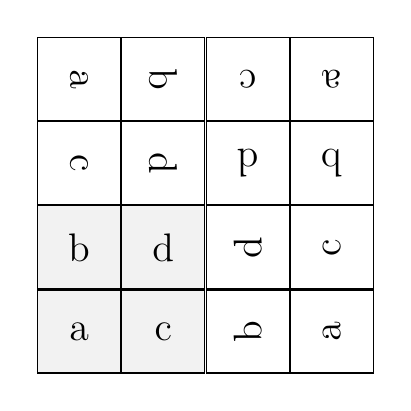
\begin{tikzpicture}[node distance=-0.7em]
    \matrix (xA) [anchor=west]
    {% 
        \node(xA1) [draw,right,font=\Large, minimum width=3em,minimum height=3em,fill=lightgray,
        , fill opacity=0.2, text opacity=1] {b} ;  \\
        \node(xA2) [draw,right,font=\Large, minimum width=3em,minimum height=3em,fill=lightgray,
        , fill opacity=0.2, text opacity=1] {a} ;  \\
    };
    \matrix (xB) [right=of xA]
    {% 
        \node(xB1) [draw,right,font=\Large, minimum width=3em,minimum height=3em,fill=lightgray,
        , fill opacity=0.2, text opacity=1] {d} ;  \\
        \node(xB2) [draw,right,font=\Large, minimum width=3em,minimum height=3em,fill=lightgray,
        , fill opacity=0.2, text opacity=1] {c} ;  \\
        %\node(xB3) [draw,anchor=west,font=\Large, minimum width=3em,minimum height=3em] {c} ;  \\
    };
    \matrix (yA) [above=of xA]
    {% 
        \node(yA1) [rotate=-90,draw,right,font=\Large, minimum width=3em,minimum height=3em] {a} ;  \\
        \node(yA2) [rotate=-90,draw,right,font=\Large, minimum width=3em,minimum height=3em] {c} ;  \\
     };
     \matrix (yB) [above=of xB]
    {% 
        \node(yB1) [rotate=-90,draw,right,font=\Large, minimum width=3em,minimum height=3em] {b} ;  \\
        \node(yB2) [rotate=-90,draw,right,font=\Large, minimum width=3em,minimum height=3em] {d} ;  \\
     };
    \matrix (xC) [right=of xB]
    {% 
        \node(xC1) [rotate=90,draw,right,font=\Large, minimum width=3em,minimum height=3em] {d} ;  \\
        \node(xC2) [rotate=90,draw,right,font=\Large, minimum width=3em,minimum height=3em] {b} ;  \\
    };
    \matrix (yC) [right=of xC]
    {% 
        \node(yC1) [rotate=90,draw,right,font=\Large, minimum width=3em,minimum height=3em] {c} ;  \\
        \node(yC2) [rotate=90,draw,right,font=\Large, minimum width=3em,minimum height=3em] {a} ;  \\
    };
 \matrix (xD) [above=of xC]
    {% 
        \node(xD1) [rotate=180,draw,right,font=\Large, minimum width=3em,minimum height=3em] {c} ;  \\
        \node(xD2) [rotate=180,draw,right,font=\Large, minimum width=3em,minimum height=3em] {d} ;  \\
    };
    \matrix (yD) [right=of xD]
    {% 
        \node(yD1) [rotate=180,draw,right,font=\Large, minimum width=3em,minimum height=3em] {a} ;  \\
        \node(yD2) [rotate=180,draw,right,font=\Large, minimum width=3em,minimum height=3em] {b} ;  \\
    };
\end{tikzpicture}} In this booklet, the core pattern is assumed to be in the lower left. Each pattern can identified as a sequence of 4 digits $abcd$ that list the rotational positions of each tile in the lower left quadrant.

\vspace{2cm}

\begin{center}
{
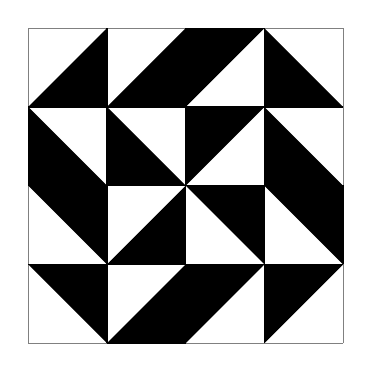
\begin{tikzpicture}[scale=1]
 \draw [step=1cm,gray,very thin](0,-1) grid (4,3); 
 \draw[opacity=1,fill=black](0,0)--(1,0)--(1,-1); 
 \draw[opacity=1,fill=black](0,1)--(1,1)--(1,0); 
 \draw[opacity=1,fill=black](1,1)--(0,1)--(0,2); 
 \draw[opacity=1,fill=black](1,3)--(1,2)--(0,2); 
 \draw[opacity=1,fill=black](2,0)--(2,-1)--(1,-1); 
 \draw[opacity=1,fill=black](2,1)--(2,0)--(1,0); 
 \draw[opacity=1,fill=black](2,1)--(1,1)--(1,2); 
 \draw[opacity=1,fill=black](2,3)--(2,2)--(1,2); 
 \draw[opacity=1,fill=black](2,-1)--(2,0)--(3,0); 
 \draw[opacity=1,fill=black](2,1)--(3,1)--(3,0); 
 \draw[opacity=1,fill=black](2,1)--(2,2)--(3,2); 
 \draw[opacity=1,fill=black](2,2)--(2,3)--(3,3); 
 \draw[opacity=1,fill=black](3,-1)--(3,0)--(4,0); 
 \draw[opacity=1,fill=black](3,1)--(4,1)--(4,0); 
 \draw[opacity=1,fill=black](4,1)--(3,1)--(3,2); 
 \draw[opacity=1,fill=black](4,2)--(3,2)--(3,3); 
\end{tikzpicture}

\textit{The 0011 pattern}
}
\end{center}

\chapter{Pattern families}

\noindent
We can group the 4x4 Truchet tile patterns with rotational symmetry into families where  tile patterns are considered to be in the same family if they would look the same without colour -- if each corresponding tile shares the same diagonal direction. The sequence that represents the family of a tile pattern can be found by taking the sequence of the tile pattern \textit{modulo} $2$. So, for example, the 16 tile patterns below are all members of the 0110 family. 

\vspace{1.2cm}

\marginnote{\centering\input{tiles/parent-0110.gtex}\\ \textit{The 0110 family pattern}}

{
\setlength{\tabcolsep}{3pt}
\renewcommand{\arraystretch}{2}
\begin{center}
\begin{tabular}{cccc} 
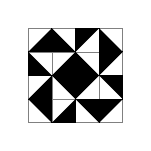
\begin{tikzpicture}[scale=0.3]
 \draw [step=1cm,gray,very thin](0,-1) grid (4,3); 
 \draw[opacity=1,fill=black](0,0)--(1,0)--(1,-1); 
 \draw[opacity=1,fill=black](1,1)--(1,0)--(0,0); 
 \draw[opacity=1,fill=black](1,1)--(0,1)--(0,2); 
 \draw[opacity=1,fill=black](1,3)--(1,2)--(0,2); 
 \draw[opacity=1,fill=black](2,0)--(2,-1)--(1,-1); 
 \draw[opacity=1,fill=black](1,1)--(2,1)--(2,0); 
 \draw[opacity=1,fill=black](2,2)--(2,1)--(1,1); 
 \draw[opacity=1,fill=black](2,2)--(1,2)--(1,3); 
 \draw[opacity=1,fill=black](2,0)--(3,0)--(3,-1); 
 \draw[opacity=1,fill=black](2,0)--(2,1)--(3,1); 
 \draw[opacity=1,fill=black](3,1)--(2,1)--(2,2); 
 \draw[opacity=1,fill=black](2,2)--(2,3)--(3,3); 
 \draw[opacity=1,fill=black](3,-1)--(3,0)--(4,0); 
 \draw[opacity=1,fill=black](3,1)--(4,1)--(4,0); 
 \draw[opacity=1,fill=black](3,1)--(3,2)--(4,2); 
 \draw[opacity=1,fill=black](4,2)--(3,2)--(3,3); 
\end{tikzpicture} 
 & 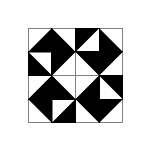
\begin{tikzpicture}[scale=0.3]
 \draw [step=1cm,gray,very thin](0,-1) grid (4,3); 
 \draw[opacity=1,fill=black](0,0)--(1,0)--(1,-1); 
 \draw[opacity=1,fill=black](1,1)--(1,0)--(0,0); 
 \draw[opacity=1,fill=black](1,1)--(0,1)--(0,2); 
 \draw[opacity=1,fill=black](1,3)--(1,2)--(0,2); 
 \draw[opacity=1,fill=black](2,0)--(2,-1)--(1,-1); 
 \draw[opacity=1,fill=black](2,0)--(1,0)--(1,1); 
 \draw[opacity=1,fill=black](1,1)--(1,2)--(2,2); 
 \draw[opacity=1,fill=black](2,2)--(1,2)--(1,3); 
 \draw[opacity=1,fill=black](2,0)--(3,0)--(3,-1); 
 \draw[opacity=1,fill=black](3,1)--(3,0)--(2,0); 
 \draw[opacity=1,fill=black](2,2)--(3,2)--(3,1); 
 \draw[opacity=1,fill=black](2,2)--(2,3)--(3,3); 
 \draw[opacity=1,fill=black](3,-1)--(3,0)--(4,0); 
 \draw[opacity=1,fill=black](3,1)--(4,1)--(4,0); 
 \draw[opacity=1,fill=black](3,1)--(3,2)--(4,2); 
 \draw[opacity=1,fill=black](4,2)--(3,2)--(3,3); 
\end{tikzpicture} 
 & 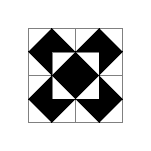
\begin{tikzpicture}[scale=0.3]
 \draw [step=1cm,gray,very thin](0,-1) grid (4,3); 
 \draw[opacity=1,fill=black](0,0)--(1,0)--(1,-1); 
 \draw[opacity=1,fill=black](1,1)--(1,0)--(0,0); 
 \draw[opacity=1,fill=black](0,2)--(1,2)--(1,1); 
 \draw[opacity=1,fill=black](1,3)--(1,2)--(0,2); 
 \draw[opacity=1,fill=black](1,-1)--(1,0)--(2,0); 
 \draw[opacity=1,fill=black](1,1)--(2,1)--(2,0); 
 \draw[opacity=1,fill=black](2,2)--(2,1)--(1,1); 
 \draw[opacity=1,fill=black](2,2)--(1,2)--(1,3); 
 \draw[opacity=1,fill=black](2,0)--(3,0)--(3,-1); 
 \draw[opacity=1,fill=black](2,0)--(2,1)--(3,1); 
 \draw[opacity=1,fill=black](3,1)--(2,1)--(2,2); 
 \draw[opacity=1,fill=black](3,3)--(3,2)--(2,2); 
 \draw[opacity=1,fill=black](3,-1)--(3,0)--(4,0); 
 \draw[opacity=1,fill=black](4,0)--(3,0)--(3,1); 
 \draw[opacity=1,fill=black](3,1)--(3,2)--(4,2); 
 \draw[opacity=1,fill=black](4,2)--(3,2)--(3,3); 
\end{tikzpicture} 
 & 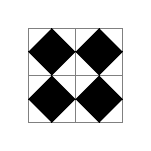
\begin{tikzpicture}[scale=0.3]
 \draw [step=1cm,gray,very thin](0,-1) grid (4,3); 
 \draw[opacity=1,fill=black](0,0)--(1,0)--(1,-1); 
 \draw[opacity=1,fill=black](1,1)--(1,0)--(0,0); 
 \draw[opacity=1,fill=black](0,2)--(1,2)--(1,1); 
 \draw[opacity=1,fill=black](1,3)--(1,2)--(0,2); 
 \draw[opacity=1,fill=black](1,-1)--(1,0)--(2,0); 
 \draw[opacity=1,fill=black](2,0)--(1,0)--(1,1); 
 \draw[opacity=1,fill=black](1,1)--(1,2)--(2,2); 
 \draw[opacity=1,fill=black](2,2)--(1,2)--(1,3); 
 \draw[opacity=1,fill=black](2,0)--(3,0)--(3,-1); 
 \draw[opacity=1,fill=black](3,1)--(3,0)--(2,0); 
 \draw[opacity=1,fill=black](2,2)--(3,2)--(3,1); 
 \draw[opacity=1,fill=black](3,3)--(3,2)--(2,2); 
 \draw[opacity=1,fill=black](3,-1)--(3,0)--(4,0); 
 \draw[opacity=1,fill=black](4,0)--(3,0)--(3,1); 
 \draw[opacity=1,fill=black](3,1)--(3,2)--(4,2); 
 \draw[opacity=1,fill=black](4,2)--(3,2)--(3,3); 
\end{tikzpicture} 
\\ 
 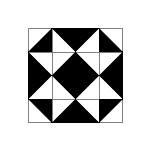
\begin{tikzpicture}[scale=0.3]
 \draw [step=1cm,gray,very thin](0,-1) grid (4,3); 
 \draw[opacity=1,fill=black](0,0)--(1,0)--(1,-1); 
 \draw[opacity=1,fill=black](0,0)--(0,1)--(1,1); 
 \draw[opacity=1,fill=black](1,1)--(0,1)--(0,2); 
 \draw[opacity=1,fill=black](1,3)--(1,2)--(0,2); 
 \draw[opacity=1,fill=black](2,0)--(2,-1)--(1,-1); 
 \draw[opacity=1,fill=black](1,1)--(2,1)--(2,0); 
 \draw[opacity=1,fill=black](2,2)--(2,1)--(1,1); 
 \draw[opacity=1,fill=black](1,3)--(2,3)--(2,2); 
 \draw[opacity=1,fill=black](3,-1)--(2,-1)--(2,0); 
 \draw[opacity=1,fill=black](2,0)--(2,1)--(3,1); 
 \draw[opacity=1,fill=black](3,1)--(2,1)--(2,2); 
 \draw[opacity=1,fill=black](2,2)--(2,3)--(3,3); 
 \draw[opacity=1,fill=black](3,-1)--(3,0)--(4,0); 
 \draw[opacity=1,fill=black](3,1)--(4,1)--(4,0); 
 \draw[opacity=1,fill=black](4,2)--(4,1)--(3,1); 
 \draw[opacity=1,fill=black](4,2)--(3,2)--(3,3); 
\end{tikzpicture} 
 & 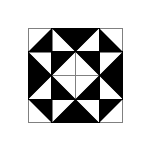
\begin{tikzpicture}[scale=0.3]
 \draw [step=1cm,gray,very thin](0,-1) grid (4,3); 
 \draw[opacity=1,fill=black](0,0)--(1,0)--(1,-1); 
 \draw[opacity=1,fill=black](0,0)--(0,1)--(1,1); 
 \draw[opacity=1,fill=black](1,1)--(0,1)--(0,2); 
 \draw[opacity=1,fill=black](1,3)--(1,2)--(0,2); 
 \draw[opacity=1,fill=black](2,0)--(2,-1)--(1,-1); 
 \draw[opacity=1,fill=black](2,0)--(1,0)--(1,1); 
 \draw[opacity=1,fill=black](1,1)--(1,2)--(2,2); 
 \draw[opacity=1,fill=black](1,3)--(2,3)--(2,2); 
 \draw[opacity=1,fill=black](3,-1)--(2,-1)--(2,0); 
 \draw[opacity=1,fill=black](3,1)--(3,0)--(2,0); 
 \draw[opacity=1,fill=black](2,2)--(3,2)--(3,1); 
 \draw[opacity=1,fill=black](2,2)--(2,3)--(3,3); 
 \draw[opacity=1,fill=black](3,-1)--(3,0)--(4,0); 
 \draw[opacity=1,fill=black](3,1)--(4,1)--(4,0); 
 \draw[opacity=1,fill=black](4,2)--(4,1)--(3,1); 
 \draw[opacity=1,fill=black](4,2)--(3,2)--(3,3); 
\end{tikzpicture} 
 & 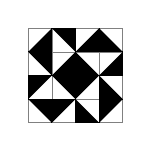
\begin{tikzpicture}[scale=0.3]
 \draw [step=1cm,gray,very thin](0,-1) grid (4,3); 
 \draw[opacity=1,fill=black](0,0)--(1,0)--(1,-1); 
 \draw[opacity=1,fill=black](0,0)--(0,1)--(1,1); 
 \draw[opacity=1,fill=black](0,2)--(1,2)--(1,1); 
 \draw[opacity=1,fill=black](1,3)--(1,2)--(0,2); 
 \draw[opacity=1,fill=black](1,-1)--(1,0)--(2,0); 
 \draw[opacity=1,fill=black](1,1)--(2,1)--(2,0); 
 \draw[opacity=1,fill=black](2,2)--(2,1)--(1,1); 
 \draw[opacity=1,fill=black](1,3)--(2,3)--(2,2); 
 \draw[opacity=1,fill=black](3,-1)--(2,-1)--(2,0); 
 \draw[opacity=1,fill=black](2,0)--(2,1)--(3,1); 
 \draw[opacity=1,fill=black](3,1)--(2,1)--(2,2); 
 \draw[opacity=1,fill=black](3,3)--(3,2)--(2,2); 
 \draw[opacity=1,fill=black](3,-1)--(3,0)--(4,0); 
 \draw[opacity=1,fill=black](4,0)--(3,0)--(3,1); 
 \draw[opacity=1,fill=black](4,2)--(4,1)--(3,1); 
 \draw[opacity=1,fill=black](4,2)--(3,2)--(3,3); 
\end{tikzpicture} 
 & 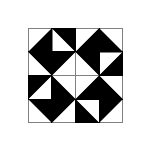
\begin{tikzpicture}[scale=0.3]
 \draw [step=1cm,gray,very thin](0,-1) grid (4,3); 
 \draw[opacity=1,fill=black](0,0)--(1,0)--(1,-1); 
 \draw[opacity=1,fill=black](0,0)--(0,1)--(1,1); 
 \draw[opacity=1,fill=black](0,2)--(1,2)--(1,1); 
 \draw[opacity=1,fill=black](1,3)--(1,2)--(0,2); 
 \draw[opacity=1,fill=black](1,-1)--(1,0)--(2,0); 
 \draw[opacity=1,fill=black](2,0)--(1,0)--(1,1); 
 \draw[opacity=1,fill=black](1,1)--(1,2)--(2,2); 
 \draw[opacity=1,fill=black](1,3)--(2,3)--(2,2); 
 \draw[opacity=1,fill=black](3,-1)--(2,-1)--(2,0); 
 \draw[opacity=1,fill=black](3,1)--(3,0)--(2,0); 
 \draw[opacity=1,fill=black](2,2)--(3,2)--(3,1); 
 \draw[opacity=1,fill=black](3,3)--(3,2)--(2,2); 
 \draw[opacity=1,fill=black](3,-1)--(3,0)--(4,0); 
 \draw[opacity=1,fill=black](4,0)--(3,0)--(3,1); 
 \draw[opacity=1,fill=black](4,2)--(4,1)--(3,1); 
 \draw[opacity=1,fill=black](4,2)--(3,2)--(3,3); 
\end{tikzpicture} 
\\ 
 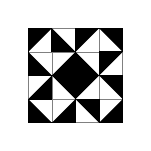
\begin{tikzpicture}[scale=0.3]
 \draw [step=1cm,gray,very thin](0,-1) grid (4,3); 
 \draw[opacity=1,fill=black](1,-1)--(0,-1)--(0,0); 
 \draw[opacity=1,fill=black](1,1)--(1,0)--(0,0); 
 \draw[opacity=1,fill=black](1,1)--(0,1)--(0,2); 
 \draw[opacity=1,fill=black](0,2)--(0,3)--(1,3); 
 \draw[opacity=1,fill=black](2,0)--(2,-1)--(1,-1); 
 \draw[opacity=1,fill=black](1,1)--(2,1)--(2,0); 
 \draw[opacity=1,fill=black](2,2)--(2,1)--(1,1); 
 \draw[opacity=1,fill=black](2,2)--(1,2)--(1,3); 
 \draw[opacity=1,fill=black](2,0)--(3,0)--(3,-1); 
 \draw[opacity=1,fill=black](2,0)--(2,1)--(3,1); 
 \draw[opacity=1,fill=black](3,1)--(2,1)--(2,2); 
 \draw[opacity=1,fill=black](2,2)--(2,3)--(3,3); 
 \draw[opacity=1,fill=black](4,0)--(4,-1)--(3,-1); 
 \draw[opacity=1,fill=black](3,1)--(4,1)--(4,0); 
 \draw[opacity=1,fill=black](3,1)--(3,2)--(4,2); 
 \draw[opacity=1,fill=black](3,3)--(4,3)--(4,2); 
\end{tikzpicture} 
 & 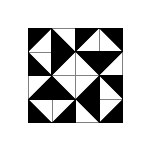
\begin{tikzpicture}[scale=0.3]
 \draw [step=1cm,gray,very thin](0,-1) grid (4,3); 
 \draw[opacity=1,fill=black](1,-1)--(0,-1)--(0,0); 
 \draw[opacity=1,fill=black](1,1)--(1,0)--(0,0); 
 \draw[opacity=1,fill=black](1,1)--(0,1)--(0,2); 
 \draw[opacity=1,fill=black](0,2)--(0,3)--(1,3); 
 \draw[opacity=1,fill=black](2,0)--(2,-1)--(1,-1); 
 \draw[opacity=1,fill=black](2,0)--(1,0)--(1,1); 
 \draw[opacity=1,fill=black](1,1)--(1,2)--(2,2); 
 \draw[opacity=1,fill=black](2,2)--(1,2)--(1,3); 
 \draw[opacity=1,fill=black](2,0)--(3,0)--(3,-1); 
 \draw[opacity=1,fill=black](3,1)--(3,0)--(2,0); 
 \draw[opacity=1,fill=black](2,2)--(3,2)--(3,1); 
 \draw[opacity=1,fill=black](2,2)--(2,3)--(3,3); 
 \draw[opacity=1,fill=black](4,0)--(4,-1)--(3,-1); 
 \draw[opacity=1,fill=black](3,1)--(4,1)--(4,0); 
 \draw[opacity=1,fill=black](3,1)--(3,2)--(4,2); 
 \draw[opacity=1,fill=black](3,3)--(4,3)--(4,2); 
\end{tikzpicture} 
 & 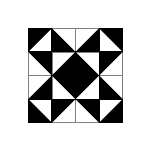
\begin{tikzpicture}[scale=0.3]
 \draw [step=1cm,gray,very thin](0,-1) grid (4,3); 
 \draw[opacity=1,fill=black](1,-1)--(0,-1)--(0,0); 
 \draw[opacity=1,fill=black](1,1)--(1,0)--(0,0); 
 \draw[opacity=1,fill=black](0,2)--(1,2)--(1,1); 
 \draw[opacity=1,fill=black](0,2)--(0,3)--(1,3); 
 \draw[opacity=1,fill=black](1,-1)--(1,0)--(2,0); 
 \draw[opacity=1,fill=black](1,1)--(2,1)--(2,0); 
 \draw[opacity=1,fill=black](2,2)--(2,1)--(1,1); 
 \draw[opacity=1,fill=black](2,2)--(1,2)--(1,3); 
 \draw[opacity=1,fill=black](2,0)--(3,0)--(3,-1); 
 \draw[opacity=1,fill=black](2,0)--(2,1)--(3,1); 
 \draw[opacity=1,fill=black](3,1)--(2,1)--(2,2); 
 \draw[opacity=1,fill=black](3,3)--(3,2)--(2,2); 
 \draw[opacity=1,fill=black](4,0)--(4,-1)--(3,-1); 
 \draw[opacity=1,fill=black](4,0)--(3,0)--(3,1); 
 \draw[opacity=1,fill=black](3,1)--(3,2)--(4,2); 
 \draw[opacity=1,fill=black](3,3)--(4,3)--(4,2); 
\end{tikzpicture} 
 & 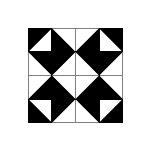
\begin{tikzpicture}[scale=0.3]
 \draw [step=1cm,gray,very thin](0,-1) grid (4,3); 
 \draw[opacity=1,fill=black](1,-1)--(0,-1)--(0,0); 
 \draw[opacity=1,fill=black](1,1)--(1,0)--(0,0); 
 \draw[opacity=1,fill=black](0,2)--(1,2)--(1,1); 
 \draw[opacity=1,fill=black](0,2)--(0,3)--(1,3); 
 \draw[opacity=1,fill=black](1,-1)--(1,0)--(2,0); 
 \draw[opacity=1,fill=black](2,0)--(1,0)--(1,1); 
 \draw[opacity=1,fill=black](1,1)--(1,2)--(2,2); 
 \draw[opacity=1,fill=black](2,2)--(1,2)--(1,3); 
 \draw[opacity=1,fill=black](2,0)--(3,0)--(3,-1); 
 \draw[opacity=1,fill=black](3,1)--(3,0)--(2,0); 
 \draw[opacity=1,fill=black](2,2)--(3,2)--(3,1); 
 \draw[opacity=1,fill=black](3,3)--(3,2)--(2,2); 
 \draw[opacity=1,fill=black](4,0)--(4,-1)--(3,-1); 
 \draw[opacity=1,fill=black](4,0)--(3,0)--(3,1); 
 \draw[opacity=1,fill=black](3,1)--(3,2)--(4,2); 
 \draw[opacity=1,fill=black](3,3)--(4,3)--(4,2); 
\end{tikzpicture} 
\\ 
 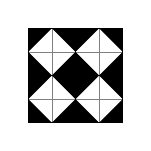
\begin{tikzpicture}[scale=0.3]
 \draw [step=1cm,gray,very thin](0,-1) grid (4,3); 
 \draw[opacity=1,fill=black](1,-1)--(0,-1)--(0,0); 
 \draw[opacity=1,fill=black](0,0)--(0,1)--(1,1); 
 \draw[opacity=1,fill=black](1,1)--(0,1)--(0,2); 
 \draw[opacity=1,fill=black](0,2)--(0,3)--(1,3); 
 \draw[opacity=1,fill=black](2,0)--(2,-1)--(1,-1); 
 \draw[opacity=1,fill=black](1,1)--(2,1)--(2,0); 
 \draw[opacity=1,fill=black](2,2)--(2,1)--(1,1); 
 \draw[opacity=1,fill=black](1,3)--(2,3)--(2,2); 
 \draw[opacity=1,fill=black](3,-1)--(2,-1)--(2,0); 
 \draw[opacity=1,fill=black](2,0)--(2,1)--(3,1); 
 \draw[opacity=1,fill=black](3,1)--(2,1)--(2,2); 
 \draw[opacity=1,fill=black](2,2)--(2,3)--(3,3); 
 \draw[opacity=1,fill=black](4,0)--(4,-1)--(3,-1); 
 \draw[opacity=1,fill=black](3,1)--(4,1)--(4,0); 
 \draw[opacity=1,fill=black](4,2)--(4,1)--(3,1); 
 \draw[opacity=1,fill=black](3,3)--(4,3)--(4,2); 
\end{tikzpicture} 
 & 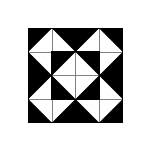
\begin{tikzpicture}[scale=0.3]
 \draw [step=1cm,gray,very thin](0,-1) grid (4,3); 
 \draw[opacity=1,fill=black](1,-1)--(0,-1)--(0,0); 
 \draw[opacity=1,fill=black](0,0)--(0,1)--(1,1); 
 \draw[opacity=1,fill=black](1,1)--(0,1)--(0,2); 
 \draw[opacity=1,fill=black](0,2)--(0,3)--(1,3); 
 \draw[opacity=1,fill=black](2,0)--(2,-1)--(1,-1); 
 \draw[opacity=1,fill=black](2,0)--(1,0)--(1,1); 
 \draw[opacity=1,fill=black](1,1)--(1,2)--(2,2); 
 \draw[opacity=1,fill=black](1,3)--(2,3)--(2,2); 
 \draw[opacity=1,fill=black](3,-1)--(2,-1)--(2,0); 
 \draw[opacity=1,fill=black](3,1)--(3,0)--(2,0); 
 \draw[opacity=1,fill=black](2,2)--(3,2)--(3,1); 
 \draw[opacity=1,fill=black](2,2)--(2,3)--(3,3); 
 \draw[opacity=1,fill=black](4,0)--(4,-1)--(3,-1); 
 \draw[opacity=1,fill=black](3,1)--(4,1)--(4,0); 
 \draw[opacity=1,fill=black](4,2)--(4,1)--(3,1); 
 \draw[opacity=1,fill=black](3,3)--(4,3)--(4,2); 
\end{tikzpicture} 
 & 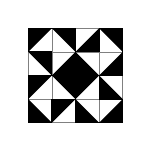
\begin{tikzpicture}[scale=0.3]
 \draw [step=1cm,gray,very thin](0,-1) grid (4,3); 
 \draw[opacity=1,fill=black](1,-1)--(0,-1)--(0,0); 
 \draw[opacity=1,fill=black](0,0)--(0,1)--(1,1); 
 \draw[opacity=1,fill=black](0,2)--(1,2)--(1,1); 
 \draw[opacity=1,fill=black](0,2)--(0,3)--(1,3); 
 \draw[opacity=1,fill=black](1,-1)--(1,0)--(2,0); 
 \draw[opacity=1,fill=black](1,1)--(2,1)--(2,0); 
 \draw[opacity=1,fill=black](2,2)--(2,1)--(1,1); 
 \draw[opacity=1,fill=black](1,3)--(2,3)--(2,2); 
 \draw[opacity=1,fill=black](3,-1)--(2,-1)--(2,0); 
 \draw[opacity=1,fill=black](2,0)--(2,1)--(3,1); 
 \draw[opacity=1,fill=black](3,1)--(2,1)--(2,2); 
 \draw[opacity=1,fill=black](3,3)--(3,2)--(2,2); 
 \draw[opacity=1,fill=black](4,0)--(4,-1)--(3,-1); 
 \draw[opacity=1,fill=black](4,0)--(3,0)--(3,1); 
 \draw[opacity=1,fill=black](4,2)--(4,1)--(3,1); 
 \draw[opacity=1,fill=black](3,3)--(4,3)--(4,2); 
\end{tikzpicture} 
 & 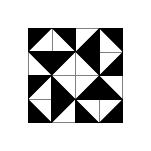
\begin{tikzpicture}[scale=0.3]
 \draw [step=1cm,gray,very thin](0,-1) grid (4,3); 
 \draw[opacity=1,fill=black](1,-1)--(0,-1)--(0,0); 
 \draw[opacity=1,fill=black](0,0)--(0,1)--(1,1); 
 \draw[opacity=1,fill=black](0,2)--(1,2)--(1,1); 
 \draw[opacity=1,fill=black](0,2)--(0,3)--(1,3); 
 \draw[opacity=1,fill=black](1,-1)--(1,0)--(2,0); 
 \draw[opacity=1,fill=black](2,0)--(1,0)--(1,1); 
 \draw[opacity=1,fill=black](1,1)--(1,2)--(2,2); 
 \draw[opacity=1,fill=black](1,3)--(2,3)--(2,2); 
 \draw[opacity=1,fill=black](3,-1)--(2,-1)--(2,0); 
 \draw[opacity=1,fill=black](3,1)--(3,0)--(2,0); 
 \draw[opacity=1,fill=black](2,2)--(3,2)--(3,1); 
 \draw[opacity=1,fill=black](3,3)--(3,2)--(2,2); 
 \draw[opacity=1,fill=black](4,0)--(4,-1)--(3,-1); 
 \draw[opacity=1,fill=black](4,0)--(3,0)--(3,1); 
 \draw[opacity=1,fill=black](4,2)--(4,1)--(3,1); 
 \draw[opacity=1,fill=black](3,3)--(4,3)--(4,2); 
\end{tikzpicture} 
\\ 
 \end{tabular} 
 \end{center}
{\begin{center} \textit{The 0110 pattern family}\end{center}}
}

\newpage

%%
% Start the main matter (normal chapters)
%\mainmatter

%\section{0000}

\vspace{1cm}
\begin{center}
\begin{tabular}{cccc} 
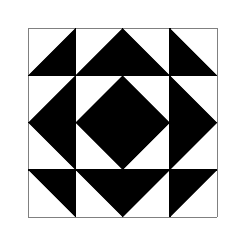
\begin{tikzpicture}[scale=0.6]
 \draw [step=1cm,gray,very thin](0,-1) grid (4,3); 
 \draw[opacity=1,fill=black](0,0)--(1,0)--(1,-1); 
 \draw[opacity=1,fill=black](0,1)--(1,1)--(1,0); 
 \draw[opacity=1,fill=black](1,2)--(1,1)--(0,1); 
 \draw[opacity=1,fill=black](1,3)--(1,2)--(0,2); 
 \draw[opacity=1,fill=black](1,0)--(2,0)--(2,-1); 
 \draw[opacity=1,fill=black](1,1)--(2,1)--(2,0); 
 \draw[opacity=1,fill=black](2,2)--(2,1)--(1,1); 
 \draw[opacity=1,fill=black](2,3)--(2,2)--(1,2); 
 \draw[opacity=1,fill=black](2,-1)--(2,0)--(3,0); 
 \draw[opacity=1,fill=black](2,0)--(2,1)--(3,1); 
 \draw[opacity=1,fill=black](3,1)--(2,1)--(2,2); 
 \draw[opacity=1,fill=black](3,2)--(2,2)--(2,3); 
 \draw[opacity=1,fill=black](3,-1)--(3,0)--(4,0); 
 \draw[opacity=1,fill=black](3,0)--(3,1)--(4,1); 
 \draw[opacity=1,fill=black](4,1)--(3,1)--(3,2); 
 \draw[opacity=1,fill=black](4,2)--(3,2)--(3,3); 
\end{tikzpicture} 
 & 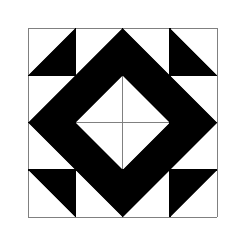
\begin{tikzpicture}[scale=0.6]
 \draw [step=1cm,gray,very thin](0,-1) grid (4,3); 
 \draw[opacity=1,fill=black](0,0)--(1,0)--(1,-1); 
 \draw[opacity=1,fill=black](0,1)--(1,1)--(1,0); 
 \draw[opacity=1,fill=black](1,2)--(1,1)--(0,1); 
 \draw[opacity=1,fill=black](1,3)--(1,2)--(0,2); 
 \draw[opacity=1,fill=black](1,0)--(2,0)--(2,-1); 
 \draw[opacity=1,fill=black](2,0)--(1,0)--(1,1); 
 \draw[opacity=1,fill=black](1,1)--(1,2)--(2,2); 
 \draw[opacity=1,fill=black](2,3)--(2,2)--(1,2); 
 \draw[opacity=1,fill=black](2,-1)--(2,0)--(3,0); 
 \draw[opacity=1,fill=black](3,1)--(3,0)--(2,0); 
 \draw[opacity=1,fill=black](2,2)--(3,2)--(3,1); 
 \draw[opacity=1,fill=black](3,2)--(2,2)--(2,3); 
 \draw[opacity=1,fill=black](3,-1)--(3,0)--(4,0); 
 \draw[opacity=1,fill=black](3,0)--(3,1)--(4,1); 
 \draw[opacity=1,fill=black](4,1)--(3,1)--(3,2); 
 \draw[opacity=1,fill=black](4,2)--(3,2)--(3,3); 
\end{tikzpicture} 
 & 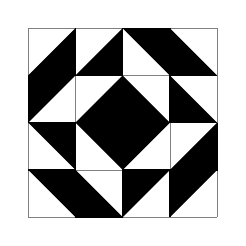
\begin{tikzpicture}[scale=0.6]
 \draw [step=1cm,gray,very thin](0,-1) grid (4,3); 
 \draw[opacity=1,fill=black](0,0)--(1,0)--(1,-1); 
 \draw[opacity=1,fill=black](0,1)--(1,1)--(1,0); 
 \draw[opacity=1,fill=black](0,1)--(0,2)--(1,2); 
 \draw[opacity=1,fill=black](1,3)--(1,2)--(0,2); 
 \draw[opacity=1,fill=black](2,-1)--(1,-1)--(1,0); 
 \draw[opacity=1,fill=black](1,1)--(2,1)--(2,0); 
 \draw[opacity=1,fill=black](2,2)--(2,1)--(1,1); 
 \draw[opacity=1,fill=black](2,3)--(2,2)--(1,2); 
 \draw[opacity=1,fill=black](2,-1)--(2,0)--(3,0); 
 \draw[opacity=1,fill=black](2,0)--(2,1)--(3,1); 
 \draw[opacity=1,fill=black](3,1)--(2,1)--(2,2); 
 \draw[opacity=1,fill=black](2,3)--(3,3)--(3,2); 
 \draw[opacity=1,fill=black](3,-1)--(3,0)--(4,0); 
 \draw[opacity=1,fill=black](4,1)--(4,0)--(3,0); 
 \draw[opacity=1,fill=black](4,1)--(3,1)--(3,2); 
 \draw[opacity=1,fill=black](4,2)--(3,2)--(3,3); 
\end{tikzpicture} 
 & 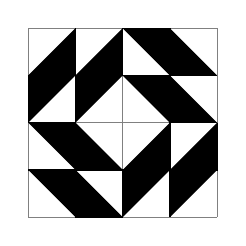
\begin{tikzpicture}[scale=0.6]
 \draw [step=1cm,gray,very thin](0,-1) grid (4,3); 
 \draw[opacity=1,fill=black](0,0)--(1,0)--(1,-1); 
 \draw[opacity=1,fill=black](0,1)--(1,1)--(1,0); 
 \draw[opacity=1,fill=black](0,1)--(0,2)--(1,2); 
 \draw[opacity=1,fill=black](1,3)--(1,2)--(0,2); 
 \draw[opacity=1,fill=black](2,-1)--(1,-1)--(1,0); 
 \draw[opacity=1,fill=black](2,0)--(1,0)--(1,1); 
 \draw[opacity=1,fill=black](1,1)--(1,2)--(2,2); 
 \draw[opacity=1,fill=black](2,3)--(2,2)--(1,2); 
 \draw[opacity=1,fill=black](2,-1)--(2,0)--(3,0); 
 \draw[opacity=1,fill=black](3,1)--(3,0)--(2,0); 
 \draw[opacity=1,fill=black](2,2)--(3,2)--(3,1); 
 \draw[opacity=1,fill=black](2,3)--(3,3)--(3,2); 
 \draw[opacity=1,fill=black](3,-1)--(3,0)--(4,0); 
 \draw[opacity=1,fill=black](4,1)--(4,0)--(3,0); 
 \draw[opacity=1,fill=black](4,1)--(3,1)--(3,2); 
 \draw[opacity=1,fill=black](4,2)--(3,2)--(3,3); 
\end{tikzpicture} 
\\ 
 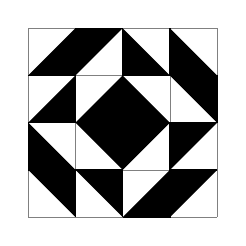
\begin{tikzpicture}[scale=0.6]
 \draw [step=1cm,gray,very thin](0,-1) grid (4,3); 
 \draw[opacity=1,fill=black](0,0)--(1,0)--(1,-1); 
 \draw[opacity=1,fill=black](1,0)--(0,0)--(0,1); 
 \draw[opacity=1,fill=black](1,2)--(1,1)--(0,1); 
 \draw[opacity=1,fill=black](1,3)--(1,2)--(0,2); 
 \draw[opacity=1,fill=black](1,0)--(2,0)--(2,-1); 
 \draw[opacity=1,fill=black](1,1)--(2,1)--(2,0); 
 \draw[opacity=1,fill=black](2,2)--(2,1)--(1,1); 
 \draw[opacity=1,fill=black](1,2)--(1,3)--(2,3); 
 \draw[opacity=1,fill=black](3,0)--(3,-1)--(2,-1); 
 \draw[opacity=1,fill=black](2,0)--(2,1)--(3,1); 
 \draw[opacity=1,fill=black](3,1)--(2,1)--(2,2); 
 \draw[opacity=1,fill=black](3,2)--(2,2)--(2,3); 
 \draw[opacity=1,fill=black](3,-1)--(3,0)--(4,0); 
 \draw[opacity=1,fill=black](3,0)--(3,1)--(4,1); 
 \draw[opacity=1,fill=black](3,2)--(4,2)--(4,1); 
 \draw[opacity=1,fill=black](4,2)--(3,2)--(3,3); 
\end{tikzpicture} 
 & 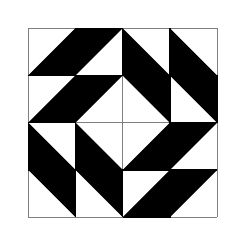
\begin{tikzpicture}[scale=0.6]
 \draw [step=1cm,gray,very thin](0,-1) grid (4,3); 
 \draw[opacity=1,fill=black](0,0)--(1,0)--(1,-1); 
 \draw[opacity=1,fill=black](1,0)--(0,0)--(0,1); 
 \draw[opacity=1,fill=black](1,2)--(1,1)--(0,1); 
 \draw[opacity=1,fill=black](1,3)--(1,2)--(0,2); 
 \draw[opacity=1,fill=black](1,0)--(2,0)--(2,-1); 
 \draw[opacity=1,fill=black](2,0)--(1,0)--(1,1); 
 \draw[opacity=1,fill=black](1,1)--(1,2)--(2,2); 
 \draw[opacity=1,fill=black](1,2)--(1,3)--(2,3); 
 \draw[opacity=1,fill=black](3,0)--(3,-1)--(2,-1); 
 \draw[opacity=1,fill=black](3,1)--(3,0)--(2,0); 
 \draw[opacity=1,fill=black](2,2)--(3,2)--(3,1); 
 \draw[opacity=1,fill=black](3,2)--(2,2)--(2,3); 
 \draw[opacity=1,fill=black](3,-1)--(3,0)--(4,0); 
 \draw[opacity=1,fill=black](3,0)--(3,1)--(4,1); 
 \draw[opacity=1,fill=black](3,2)--(4,2)--(4,1); 
 \draw[opacity=1,fill=black](4,2)--(3,2)--(3,3); 
\end{tikzpicture} 
 & 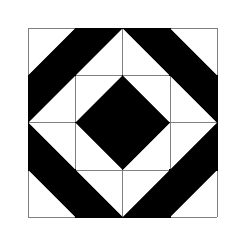
\begin{tikzpicture}[scale=0.6]
 \draw [step=1cm,gray,very thin](0,-1) grid (4,3); 
 \draw[opacity=1,fill=black](0,0)--(1,0)--(1,-1); 
 \draw[opacity=1,fill=black](1,0)--(0,0)--(0,1); 
 \draw[opacity=1,fill=black](0,1)--(0,2)--(1,2); 
 \draw[opacity=1,fill=black](1,3)--(1,2)--(0,2); 
 \draw[opacity=1,fill=black](2,-1)--(1,-1)--(1,0); 
 \draw[opacity=1,fill=black](1,1)--(2,1)--(2,0); 
 \draw[opacity=1,fill=black](2,2)--(2,1)--(1,1); 
 \draw[opacity=1,fill=black](1,2)--(1,3)--(2,3); 
 \draw[opacity=1,fill=black](3,0)--(3,-1)--(2,-1); 
 \draw[opacity=1,fill=black](2,0)--(2,1)--(3,1); 
 \draw[opacity=1,fill=black](3,1)--(2,1)--(2,2); 
 \draw[opacity=1,fill=black](2,3)--(3,3)--(3,2); 
 \draw[opacity=1,fill=black](3,-1)--(3,0)--(4,0); 
 \draw[opacity=1,fill=black](4,1)--(4,0)--(3,0); 
 \draw[opacity=1,fill=black](3,2)--(4,2)--(4,1); 
 \draw[opacity=1,fill=black](4,2)--(3,2)--(3,3); 
\end{tikzpicture} 
 & 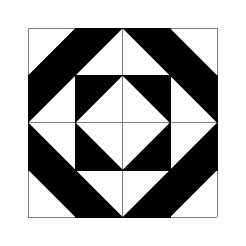
\begin{tikzpicture}[scale=0.6]
 \draw [step=1cm,gray,very thin](0,-1) grid (4,3); 
 \draw[opacity=1,fill=black](0,0)--(1,0)--(1,-1); 
 \draw[opacity=1,fill=black](1,0)--(0,0)--(0,1); 
 \draw[opacity=1,fill=black](0,1)--(0,2)--(1,2); 
 \draw[opacity=1,fill=black](1,3)--(1,2)--(0,2); 
 \draw[opacity=1,fill=black](2,-1)--(1,-1)--(1,0); 
 \draw[opacity=1,fill=black](2,0)--(1,0)--(1,1); 
 \draw[opacity=1,fill=black](1,1)--(1,2)--(2,2); 
 \draw[opacity=1,fill=black](1,2)--(1,3)--(2,3); 
 \draw[opacity=1,fill=black](3,0)--(3,-1)--(2,-1); 
 \draw[opacity=1,fill=black](3,1)--(3,0)--(2,0); 
 \draw[opacity=1,fill=black](2,2)--(3,2)--(3,1); 
 \draw[opacity=1,fill=black](2,3)--(3,3)--(3,2); 
 \draw[opacity=1,fill=black](3,-1)--(3,0)--(4,0); 
 \draw[opacity=1,fill=black](4,1)--(4,0)--(3,0); 
 \draw[opacity=1,fill=black](3,2)--(4,2)--(4,1); 
 \draw[opacity=1,fill=black](4,2)--(3,2)--(3,3); 
\end{tikzpicture} 
\\ 
 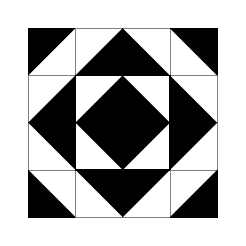
\begin{tikzpicture}[scale=0.6]
 \draw [step=1cm,gray,very thin](0,-1) grid (4,3); 
 \draw[opacity=1,fill=black](1,-1)--(0,-1)--(0,0); 
 \draw[opacity=1,fill=black](0,1)--(1,1)--(1,0); 
 \draw[opacity=1,fill=black](1,2)--(1,1)--(0,1); 
 \draw[opacity=1,fill=black](0,2)--(0,3)--(1,3); 
 \draw[opacity=1,fill=black](1,0)--(2,0)--(2,-1); 
 \draw[opacity=1,fill=black](1,1)--(2,1)--(2,0); 
 \draw[opacity=1,fill=black](2,2)--(2,1)--(1,1); 
 \draw[opacity=1,fill=black](2,3)--(2,2)--(1,2); 
 \draw[opacity=1,fill=black](2,-1)--(2,0)--(3,0); 
 \draw[opacity=1,fill=black](2,0)--(2,1)--(3,1); 
 \draw[opacity=1,fill=black](3,1)--(2,1)--(2,2); 
 \draw[opacity=1,fill=black](3,2)--(2,2)--(2,3); 
 \draw[opacity=1,fill=black](4,0)--(4,-1)--(3,-1); 
 \draw[opacity=1,fill=black](3,0)--(3,1)--(4,1); 
 \draw[opacity=1,fill=black](4,1)--(3,1)--(3,2); 
 \draw[opacity=1,fill=black](3,3)--(4,3)--(4,2); 
\end{tikzpicture} 
 & 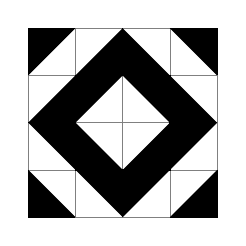
\begin{tikzpicture}[scale=0.6]
 \draw [step=1cm,gray,very thin](0,-1) grid (4,3); 
 \draw[opacity=1,fill=black](1,-1)--(0,-1)--(0,0); 
 \draw[opacity=1,fill=black](0,1)--(1,1)--(1,0); 
 \draw[opacity=1,fill=black](1,2)--(1,1)--(0,1); 
 \draw[opacity=1,fill=black](0,2)--(0,3)--(1,3); 
 \draw[opacity=1,fill=black](1,0)--(2,0)--(2,-1); 
 \draw[opacity=1,fill=black](2,0)--(1,0)--(1,1); 
 \draw[opacity=1,fill=black](1,1)--(1,2)--(2,2); 
 \draw[opacity=1,fill=black](2,3)--(2,2)--(1,2); 
 \draw[opacity=1,fill=black](2,-1)--(2,0)--(3,0); 
 \draw[opacity=1,fill=black](3,1)--(3,0)--(2,0); 
 \draw[opacity=1,fill=black](2,2)--(3,2)--(3,1); 
 \draw[opacity=1,fill=black](3,2)--(2,2)--(2,3); 
 \draw[opacity=1,fill=black](4,0)--(4,-1)--(3,-1); 
 \draw[opacity=1,fill=black](3,0)--(3,1)--(4,1); 
 \draw[opacity=1,fill=black](4,1)--(3,1)--(3,2); 
 \draw[opacity=1,fill=black](3,3)--(4,3)--(4,2); 
\end{tikzpicture} 
 & 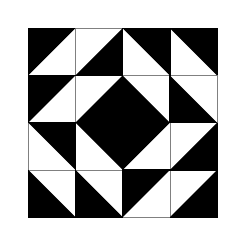
\begin{tikzpicture}[scale=0.6]
 \draw [step=1cm,gray,very thin](0,-1) grid (4,3); 
 \draw[opacity=1,fill=black](1,-1)--(0,-1)--(0,0); 
 \draw[opacity=1,fill=black](0,1)--(1,1)--(1,0); 
 \draw[opacity=1,fill=black](0,1)--(0,2)--(1,2); 
 \draw[opacity=1,fill=black](0,2)--(0,3)--(1,3); 
 \draw[opacity=1,fill=black](2,-1)--(1,-1)--(1,0); 
 \draw[opacity=1,fill=black](1,1)--(2,1)--(2,0); 
 \draw[opacity=1,fill=black](2,2)--(2,1)--(1,1); 
 \draw[opacity=1,fill=black](2,3)--(2,2)--(1,2); 
 \draw[opacity=1,fill=black](2,-1)--(2,0)--(3,0); 
 \draw[opacity=1,fill=black](2,0)--(2,1)--(3,1); 
 \draw[opacity=1,fill=black](3,1)--(2,1)--(2,2); 
 \draw[opacity=1,fill=black](2,3)--(3,3)--(3,2); 
 \draw[opacity=1,fill=black](4,0)--(4,-1)--(3,-1); 
 \draw[opacity=1,fill=black](4,1)--(4,0)--(3,0); 
 \draw[opacity=1,fill=black](4,1)--(3,1)--(3,2); 
 \draw[opacity=1,fill=black](3,3)--(4,3)--(4,2); 
\end{tikzpicture} 
 & 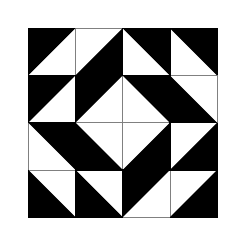
\begin{tikzpicture}[scale=0.6]
 \draw [step=1cm,gray,very thin](0,-1) grid (4,3); 
 \draw[opacity=1,fill=black](1,-1)--(0,-1)--(0,0); 
 \draw[opacity=1,fill=black](0,1)--(1,1)--(1,0); 
 \draw[opacity=1,fill=black](0,1)--(0,2)--(1,2); 
 \draw[opacity=1,fill=black](0,2)--(0,3)--(1,3); 
 \draw[opacity=1,fill=black](2,-1)--(1,-1)--(1,0); 
 \draw[opacity=1,fill=black](2,0)--(1,0)--(1,1); 
 \draw[opacity=1,fill=black](1,1)--(1,2)--(2,2); 
 \draw[opacity=1,fill=black](2,3)--(2,2)--(1,2); 
 \draw[opacity=1,fill=black](2,-1)--(2,0)--(3,0); 
 \draw[opacity=1,fill=black](3,1)--(3,0)--(2,0); 
 \draw[opacity=1,fill=black](2,2)--(3,2)--(3,1); 
 \draw[opacity=1,fill=black](2,3)--(3,3)--(3,2); 
 \draw[opacity=1,fill=black](4,0)--(4,-1)--(3,-1); 
 \draw[opacity=1,fill=black](4,1)--(4,0)--(3,0); 
 \draw[opacity=1,fill=black](4,1)--(3,1)--(3,2); 
 \draw[opacity=1,fill=black](3,3)--(4,3)--(4,2); 
\end{tikzpicture} 
\\ 
 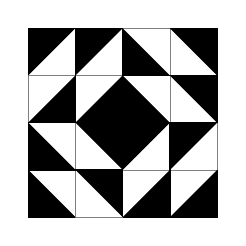
\begin{tikzpicture}[scale=0.6]
 \draw [step=1cm,gray,very thin](0,-1) grid (4,3); 
 \draw[opacity=1,fill=black](1,-1)--(0,-1)--(0,0); 
 \draw[opacity=1,fill=black](1,0)--(0,0)--(0,1); 
 \draw[opacity=1,fill=black](1,2)--(1,1)--(0,1); 
 \draw[opacity=1,fill=black](0,2)--(0,3)--(1,3); 
 \draw[opacity=1,fill=black](1,0)--(2,0)--(2,-1); 
 \draw[opacity=1,fill=black](1,1)--(2,1)--(2,0); 
 \draw[opacity=1,fill=black](2,2)--(2,1)--(1,1); 
 \draw[opacity=1,fill=black](1,2)--(1,3)--(2,3); 
 \draw[opacity=1,fill=black](3,0)--(3,-1)--(2,-1); 
 \draw[opacity=1,fill=black](2,0)--(2,1)--(3,1); 
 \draw[opacity=1,fill=black](3,1)--(2,1)--(2,2); 
 \draw[opacity=1,fill=black](3,2)--(2,2)--(2,3); 
 \draw[opacity=1,fill=black](4,0)--(4,-1)--(3,-1); 
 \draw[opacity=1,fill=black](3,0)--(3,1)--(4,1); 
 \draw[opacity=1,fill=black](3,2)--(4,2)--(4,1); 
 \draw[opacity=1,fill=black](3,3)--(4,3)--(4,2); 
\end{tikzpicture} 
 & 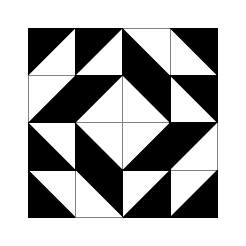
\begin{tikzpicture}[scale=0.6]
 \draw [step=1cm,gray,very thin](0,-1) grid (4,3); 
 \draw[opacity=1,fill=black](1,-1)--(0,-1)--(0,0); 
 \draw[opacity=1,fill=black](1,0)--(0,0)--(0,1); 
 \draw[opacity=1,fill=black](1,2)--(1,1)--(0,1); 
 \draw[opacity=1,fill=black](0,2)--(0,3)--(1,3); 
 \draw[opacity=1,fill=black](1,0)--(2,0)--(2,-1); 
 \draw[opacity=1,fill=black](2,0)--(1,0)--(1,1); 
 \draw[opacity=1,fill=black](1,1)--(1,2)--(2,2); 
 \draw[opacity=1,fill=black](1,2)--(1,3)--(2,3); 
 \draw[opacity=1,fill=black](3,0)--(3,-1)--(2,-1); 
 \draw[opacity=1,fill=black](3,1)--(3,0)--(2,0); 
 \draw[opacity=1,fill=black](2,2)--(3,2)--(3,1); 
 \draw[opacity=1,fill=black](3,2)--(2,2)--(2,3); 
 \draw[opacity=1,fill=black](4,0)--(4,-1)--(3,-1); 
 \draw[opacity=1,fill=black](3,0)--(3,1)--(4,1); 
 \draw[opacity=1,fill=black](3,2)--(4,2)--(4,1); 
 \draw[opacity=1,fill=black](3,3)--(4,3)--(4,2); 
\end{tikzpicture} 
 & 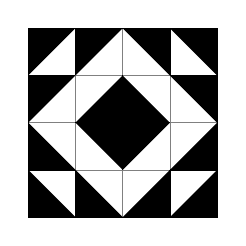
\begin{tikzpicture}[scale=0.6]
 \draw [step=1cm,gray,very thin](0,-1) grid (4,3); 
 \draw[opacity=1,fill=black](1,-1)--(0,-1)--(0,0); 
 \draw[opacity=1,fill=black](1,0)--(0,0)--(0,1); 
 \draw[opacity=1,fill=black](0,1)--(0,2)--(1,2); 
 \draw[opacity=1,fill=black](0,2)--(0,3)--(1,3); 
 \draw[opacity=1,fill=black](2,-1)--(1,-1)--(1,0); 
 \draw[opacity=1,fill=black](1,1)--(2,1)--(2,0); 
 \draw[opacity=1,fill=black](2,2)--(2,1)--(1,1); 
 \draw[opacity=1,fill=black](1,2)--(1,3)--(2,3); 
 \draw[opacity=1,fill=black](3,0)--(3,-1)--(2,-1); 
 \draw[opacity=1,fill=black](2,0)--(2,1)--(3,1); 
 \draw[opacity=1,fill=black](3,1)--(2,1)--(2,2); 
 \draw[opacity=1,fill=black](2,3)--(3,3)--(3,2); 
 \draw[opacity=1,fill=black](4,0)--(4,-1)--(3,-1); 
 \draw[opacity=1,fill=black](4,1)--(4,0)--(3,0); 
 \draw[opacity=1,fill=black](3,2)--(4,2)--(4,1); 
 \draw[opacity=1,fill=black](3,3)--(4,3)--(4,2); 
\end{tikzpicture} 
 & 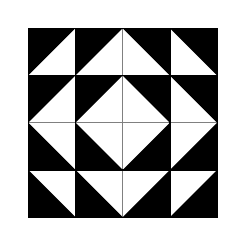
\begin{tikzpicture}[scale=0.6]
 \draw [step=1cm,gray,very thin](0,-1) grid (4,3); 
 \draw[opacity=1,fill=black](1,-1)--(0,-1)--(0,0); 
 \draw[opacity=1,fill=black](1,0)--(0,0)--(0,1); 
 \draw[opacity=1,fill=black](0,1)--(0,2)--(1,2); 
 \draw[opacity=1,fill=black](0,2)--(0,3)--(1,3); 
 \draw[opacity=1,fill=black](2,-1)--(1,-1)--(1,0); 
 \draw[opacity=1,fill=black](2,0)--(1,0)--(1,1); 
 \draw[opacity=1,fill=black](1,1)--(1,2)--(2,2); 
 \draw[opacity=1,fill=black](1,2)--(1,3)--(2,3); 
 \draw[opacity=1,fill=black](3,0)--(3,-1)--(2,-1); 
 \draw[opacity=1,fill=black](3,1)--(3,0)--(2,0); 
 \draw[opacity=1,fill=black](2,2)--(3,2)--(3,1); 
 \draw[opacity=1,fill=black](2,3)--(3,3)--(3,2); 
 \draw[opacity=1,fill=black](4,0)--(4,-1)--(3,-1); 
 \draw[opacity=1,fill=black](4,1)--(4,0)--(3,0); 
 \draw[opacity=1,fill=black](3,2)--(4,2)--(4,1); 
 \draw[opacity=1,fill=black](3,3)--(4,3)--(4,2); 
\end{tikzpicture} 
\\ 
 \end{tabular} 
\vspace{1cm}
{\Large
\begin{tabular}{cccc} 
0000 & 0002 & 0020 & 0022\\ 
 0200 & 0202 & 0220 & 0222\\ 
 2000 & 2002 & 2020 & 2022\\ 
 2200 & 2202 & 2220 & 2222\\ 
 \end{tabular} 
}
\end{center}

\newpage



\section{0001}

\vspace{1cm}
\begin{center}
\begin{tabular}{cccc} 
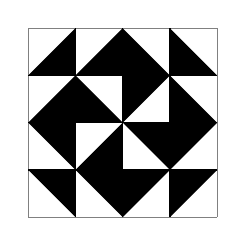
\begin{tikzpicture}[scale=0.6]
 \draw [step=1cm,gray,very thin](0,-1) grid (4,3); 
 \draw[opacity=1,fill=black](0,0)--(1,0)--(1,-1); 
 \draw[opacity=1,fill=black](0,1)--(1,1)--(1,0); 
 \draw[opacity=1,fill=black](1,2)--(1,1)--(0,1); 
 \draw[opacity=1,fill=black](1,3)--(1,2)--(0,2); 
 \draw[opacity=1,fill=black](1,0)--(2,0)--(2,-1); 
 \draw[opacity=1,fill=black](2,1)--(2,0)--(1,0); 
 \draw[opacity=1,fill=black](2,1)--(1,1)--(1,2); 
 \draw[opacity=1,fill=black](2,3)--(2,2)--(1,2); 
 \draw[opacity=1,fill=black](2,-1)--(2,0)--(3,0); 
 \draw[opacity=1,fill=black](2,1)--(3,1)--(3,0); 
 \draw[opacity=1,fill=black](2,1)--(2,2)--(3,2); 
 \draw[opacity=1,fill=black](3,2)--(2,2)--(2,3); 
 \draw[opacity=1,fill=black](3,-1)--(3,0)--(4,0); 
 \draw[opacity=1,fill=black](3,0)--(3,1)--(4,1); 
 \draw[opacity=1,fill=black](4,1)--(3,1)--(3,2); 
 \draw[opacity=1,fill=black](4,2)--(3,2)--(3,3); 
\end{tikzpicture} 
 & 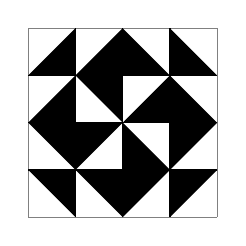
\begin{tikzpicture}[scale=0.6]
 \draw [step=1cm,gray,very thin](0,-1) grid (4,3); 
 \draw[opacity=1,fill=black](0,0)--(1,0)--(1,-1); 
 \draw[opacity=1,fill=black](0,1)--(1,1)--(1,0); 
 \draw[opacity=1,fill=black](1,2)--(1,1)--(0,1); 
 \draw[opacity=1,fill=black](1,3)--(1,2)--(0,2); 
 \draw[opacity=1,fill=black](1,0)--(2,0)--(2,-1); 
 \draw[opacity=1,fill=black](1,0)--(1,1)--(2,1); 
 \draw[opacity=1,fill=black](1,2)--(2,2)--(2,1); 
 \draw[opacity=1,fill=black](2,3)--(2,2)--(1,2); 
 \draw[opacity=1,fill=black](2,-1)--(2,0)--(3,0); 
 \draw[opacity=1,fill=black](3,0)--(2,0)--(2,1); 
 \draw[opacity=1,fill=black](3,2)--(3,1)--(2,1); 
 \draw[opacity=1,fill=black](3,2)--(2,2)--(2,3); 
 \draw[opacity=1,fill=black](3,-1)--(3,0)--(4,0); 
 \draw[opacity=1,fill=black](3,0)--(3,1)--(4,1); 
 \draw[opacity=1,fill=black](4,1)--(3,1)--(3,2); 
 \draw[opacity=1,fill=black](4,2)--(3,2)--(3,3); 
\end{tikzpicture} 
 & 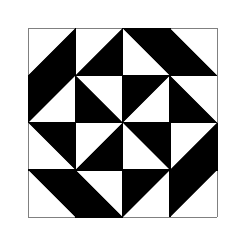
\begin{tikzpicture}[scale=0.6]
 \draw [step=1cm,gray,very thin](0,-1) grid (4,3); 
 \draw[opacity=1,fill=black](0,0)--(1,0)--(1,-1); 
 \draw[opacity=1,fill=black](0,1)--(1,1)--(1,0); 
 \draw[opacity=1,fill=black](0,1)--(0,2)--(1,2); 
 \draw[opacity=1,fill=black](1,3)--(1,2)--(0,2); 
 \draw[opacity=1,fill=black](2,-1)--(1,-1)--(1,0); 
 \draw[opacity=1,fill=black](2,1)--(2,0)--(1,0); 
 \draw[opacity=1,fill=black](2,1)--(1,1)--(1,2); 
 \draw[opacity=1,fill=black](2,3)--(2,2)--(1,2); 
 \draw[opacity=1,fill=black](2,-1)--(2,0)--(3,0); 
 \draw[opacity=1,fill=black](2,1)--(3,1)--(3,0); 
 \draw[opacity=1,fill=black](2,1)--(2,2)--(3,2); 
 \draw[opacity=1,fill=black](2,3)--(3,3)--(3,2); 
 \draw[opacity=1,fill=black](3,-1)--(3,0)--(4,0); 
 \draw[opacity=1,fill=black](4,1)--(4,0)--(3,0); 
 \draw[opacity=1,fill=black](4,1)--(3,1)--(3,2); 
 \draw[opacity=1,fill=black](4,2)--(3,2)--(3,3); 
\end{tikzpicture} 
 & 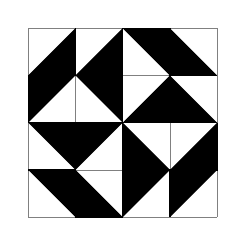
\begin{tikzpicture}[scale=0.6]
 \draw [step=1cm,gray,very thin](0,-1) grid (4,3); 
 \draw[opacity=1,fill=black](0,0)--(1,0)--(1,-1); 
 \draw[opacity=1,fill=black](0,1)--(1,1)--(1,0); 
 \draw[opacity=1,fill=black](0,1)--(0,2)--(1,2); 
 \draw[opacity=1,fill=black](1,3)--(1,2)--(0,2); 
 \draw[opacity=1,fill=black](2,-1)--(1,-1)--(1,0); 
 \draw[opacity=1,fill=black](1,0)--(1,1)--(2,1); 
 \draw[opacity=1,fill=black](1,2)--(2,2)--(2,1); 
 \draw[opacity=1,fill=black](2,3)--(2,2)--(1,2); 
 \draw[opacity=1,fill=black](2,-1)--(2,0)--(3,0); 
 \draw[opacity=1,fill=black](3,0)--(2,0)--(2,1); 
 \draw[opacity=1,fill=black](3,2)--(3,1)--(2,1); 
 \draw[opacity=1,fill=black](2,3)--(3,3)--(3,2); 
 \draw[opacity=1,fill=black](3,-1)--(3,0)--(4,0); 
 \draw[opacity=1,fill=black](4,1)--(4,0)--(3,0); 
 \draw[opacity=1,fill=black](4,1)--(3,1)--(3,2); 
 \draw[opacity=1,fill=black](4,2)--(3,2)--(3,3); 
\end{tikzpicture} 
\\ 
 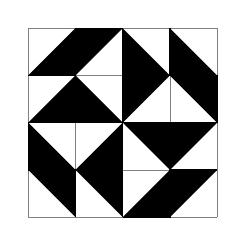
\begin{tikzpicture}[scale=0.6]
 \draw [step=1cm,gray,very thin](0,-1) grid (4,3); 
 \draw[opacity=1,fill=black](0,0)--(1,0)--(1,-1); 
 \draw[opacity=1,fill=black](1,0)--(0,0)--(0,1); 
 \draw[opacity=1,fill=black](1,2)--(1,1)--(0,1); 
 \draw[opacity=1,fill=black](1,3)--(1,2)--(0,2); 
 \draw[opacity=1,fill=black](1,0)--(2,0)--(2,-1); 
 \draw[opacity=1,fill=black](2,1)--(2,0)--(1,0); 
 \draw[opacity=1,fill=black](2,1)--(1,1)--(1,2); 
 \draw[opacity=1,fill=black](1,2)--(1,3)--(2,3); 
 \draw[opacity=1,fill=black](3,0)--(3,-1)--(2,-1); 
 \draw[opacity=1,fill=black](2,1)--(3,1)--(3,0); 
 \draw[opacity=1,fill=black](2,1)--(2,2)--(3,2); 
 \draw[opacity=1,fill=black](3,2)--(2,2)--(2,3); 
 \draw[opacity=1,fill=black](3,-1)--(3,0)--(4,0); 
 \draw[opacity=1,fill=black](3,0)--(3,1)--(4,1); 
 \draw[opacity=1,fill=black](3,2)--(4,2)--(4,1); 
 \draw[opacity=1,fill=black](4,2)--(3,2)--(3,3); 
\end{tikzpicture} 
 & 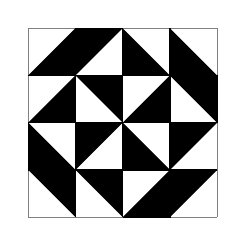
\begin{tikzpicture}[scale=0.6]
 \draw [step=1cm,gray,very thin](0,-1) grid (4,3); 
 \draw[opacity=1,fill=black](0,0)--(1,0)--(1,-1); 
 \draw[opacity=1,fill=black](1,0)--(0,0)--(0,1); 
 \draw[opacity=1,fill=black](1,2)--(1,1)--(0,1); 
 \draw[opacity=1,fill=black](1,3)--(1,2)--(0,2); 
 \draw[opacity=1,fill=black](1,0)--(2,0)--(2,-1); 
 \draw[opacity=1,fill=black](1,0)--(1,1)--(2,1); 
 \draw[opacity=1,fill=black](1,2)--(2,2)--(2,1); 
 \draw[opacity=1,fill=black](1,2)--(1,3)--(2,3); 
 \draw[opacity=1,fill=black](3,0)--(3,-1)--(2,-1); 
 \draw[opacity=1,fill=black](3,0)--(2,0)--(2,1); 
 \draw[opacity=1,fill=black](3,2)--(3,1)--(2,1); 
 \draw[opacity=1,fill=black](3,2)--(2,2)--(2,3); 
 \draw[opacity=1,fill=black](3,-1)--(3,0)--(4,0); 
 \draw[opacity=1,fill=black](3,0)--(3,1)--(4,1); 
 \draw[opacity=1,fill=black](3,2)--(4,2)--(4,1); 
 \draw[opacity=1,fill=black](4,2)--(3,2)--(3,3); 
\end{tikzpicture} 
 & 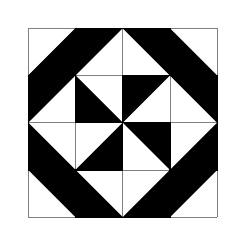
\begin{tikzpicture}[scale=0.6]
 \draw [step=1cm,gray,very thin](0,-1) grid (4,3); 
 \draw[opacity=1,fill=black](0,0)--(1,0)--(1,-1); 
 \draw[opacity=1,fill=black](1,0)--(0,0)--(0,1); 
 \draw[opacity=1,fill=black](0,1)--(0,2)--(1,2); 
 \draw[opacity=1,fill=black](1,3)--(1,2)--(0,2); 
 \draw[opacity=1,fill=black](2,-1)--(1,-1)--(1,0); 
 \draw[opacity=1,fill=black](2,1)--(2,0)--(1,0); 
 \draw[opacity=1,fill=black](2,1)--(1,1)--(1,2); 
 \draw[opacity=1,fill=black](1,2)--(1,3)--(2,3); 
 \draw[opacity=1,fill=black](3,0)--(3,-1)--(2,-1); 
 \draw[opacity=1,fill=black](2,1)--(3,1)--(3,0); 
 \draw[opacity=1,fill=black](2,1)--(2,2)--(3,2); 
 \draw[opacity=1,fill=black](2,3)--(3,3)--(3,2); 
 \draw[opacity=1,fill=black](3,-1)--(3,0)--(4,0); 
 \draw[opacity=1,fill=black](4,1)--(4,0)--(3,0); 
 \draw[opacity=1,fill=black](3,2)--(4,2)--(4,1); 
 \draw[opacity=1,fill=black](4,2)--(3,2)--(3,3); 
\end{tikzpicture} 
 & 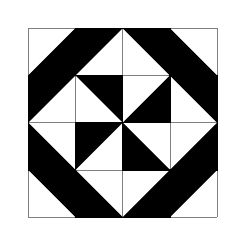
\begin{tikzpicture}[scale=0.6]
 \draw [step=1cm,gray,very thin](0,-1) grid (4,3); 
 \draw[opacity=1,fill=black](0,0)--(1,0)--(1,-1); 
 \draw[opacity=1,fill=black](1,0)--(0,0)--(0,1); 
 \draw[opacity=1,fill=black](0,1)--(0,2)--(1,2); 
 \draw[opacity=1,fill=black](1,3)--(1,2)--(0,2); 
 \draw[opacity=1,fill=black](2,-1)--(1,-1)--(1,0); 
 \draw[opacity=1,fill=black](1,0)--(1,1)--(2,1); 
 \draw[opacity=1,fill=black](1,2)--(2,2)--(2,1); 
 \draw[opacity=1,fill=black](1,2)--(1,3)--(2,3); 
 \draw[opacity=1,fill=black](3,0)--(3,-1)--(2,-1); 
 \draw[opacity=1,fill=black](3,0)--(2,0)--(2,1); 
 \draw[opacity=1,fill=black](3,2)--(3,1)--(2,1); 
 \draw[opacity=1,fill=black](2,3)--(3,3)--(3,2); 
 \draw[opacity=1,fill=black](3,-1)--(3,0)--(4,0); 
 \draw[opacity=1,fill=black](4,1)--(4,0)--(3,0); 
 \draw[opacity=1,fill=black](3,2)--(4,2)--(4,1); 
 \draw[opacity=1,fill=black](4,2)--(3,2)--(3,3); 
\end{tikzpicture} 
\\ 
 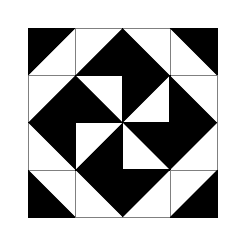
\begin{tikzpicture}[scale=0.6]
 \draw [step=1cm,gray,very thin](0,-1) grid (4,3); 
 \draw[opacity=1,fill=black](1,-1)--(0,-1)--(0,0); 
 \draw[opacity=1,fill=black](0,1)--(1,1)--(1,0); 
 \draw[opacity=1,fill=black](1,2)--(1,1)--(0,1); 
 \draw[opacity=1,fill=black](0,2)--(0,3)--(1,3); 
 \draw[opacity=1,fill=black](1,0)--(2,0)--(2,-1); 
 \draw[opacity=1,fill=black](2,1)--(2,0)--(1,0); 
 \draw[opacity=1,fill=black](2,1)--(1,1)--(1,2); 
 \draw[opacity=1,fill=black](2,3)--(2,2)--(1,2); 
 \draw[opacity=1,fill=black](2,-1)--(2,0)--(3,0); 
 \draw[opacity=1,fill=black](2,1)--(3,1)--(3,0); 
 \draw[opacity=1,fill=black](2,1)--(2,2)--(3,2); 
 \draw[opacity=1,fill=black](3,2)--(2,2)--(2,3); 
 \draw[opacity=1,fill=black](4,0)--(4,-1)--(3,-1); 
 \draw[opacity=1,fill=black](3,0)--(3,1)--(4,1); 
 \draw[opacity=1,fill=black](4,1)--(3,1)--(3,2); 
 \draw[opacity=1,fill=black](3,3)--(4,3)--(4,2); 
\end{tikzpicture} 
 & 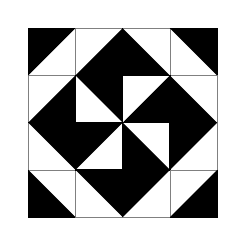
\begin{tikzpicture}[scale=0.6]
 \draw [step=1cm,gray,very thin](0,-1) grid (4,3); 
 \draw[opacity=1,fill=black](1,-1)--(0,-1)--(0,0); 
 \draw[opacity=1,fill=black](0,1)--(1,1)--(1,0); 
 \draw[opacity=1,fill=black](1,2)--(1,1)--(0,1); 
 \draw[opacity=1,fill=black](0,2)--(0,3)--(1,3); 
 \draw[opacity=1,fill=black](1,0)--(2,0)--(2,-1); 
 \draw[opacity=1,fill=black](1,0)--(1,1)--(2,1); 
 \draw[opacity=1,fill=black](1,2)--(2,2)--(2,1); 
 \draw[opacity=1,fill=black](2,3)--(2,2)--(1,2); 
 \draw[opacity=1,fill=black](2,-1)--(2,0)--(3,0); 
 \draw[opacity=1,fill=black](3,0)--(2,0)--(2,1); 
 \draw[opacity=1,fill=black](3,2)--(3,1)--(2,1); 
 \draw[opacity=1,fill=black](3,2)--(2,2)--(2,3); 
 \draw[opacity=1,fill=black](4,0)--(4,-1)--(3,-1); 
 \draw[opacity=1,fill=black](3,0)--(3,1)--(4,1); 
 \draw[opacity=1,fill=black](4,1)--(3,1)--(3,2); 
 \draw[opacity=1,fill=black](3,3)--(4,3)--(4,2); 
\end{tikzpicture} 
 & 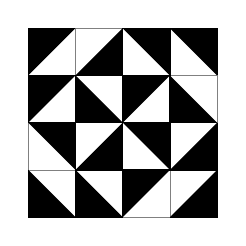
\begin{tikzpicture}[scale=0.6]
 \draw [step=1cm,gray,very thin](0,-1) grid (4,3); 
 \draw[opacity=1,fill=black](1,-1)--(0,-1)--(0,0); 
 \draw[opacity=1,fill=black](0,1)--(1,1)--(1,0); 
 \draw[opacity=1,fill=black](0,1)--(0,2)--(1,2); 
 \draw[opacity=1,fill=black](0,2)--(0,3)--(1,3); 
 \draw[opacity=1,fill=black](2,-1)--(1,-1)--(1,0); 
 \draw[opacity=1,fill=black](2,1)--(2,0)--(1,0); 
 \draw[opacity=1,fill=black](2,1)--(1,1)--(1,2); 
 \draw[opacity=1,fill=black](2,3)--(2,2)--(1,2); 
 \draw[opacity=1,fill=black](2,-1)--(2,0)--(3,0); 
 \draw[opacity=1,fill=black](2,1)--(3,1)--(3,0); 
 \draw[opacity=1,fill=black](2,1)--(2,2)--(3,2); 
 \draw[opacity=1,fill=black](2,3)--(3,3)--(3,2); 
 \draw[opacity=1,fill=black](4,0)--(4,-1)--(3,-1); 
 \draw[opacity=1,fill=black](4,1)--(4,0)--(3,0); 
 \draw[opacity=1,fill=black](4,1)--(3,1)--(3,2); 
 \draw[opacity=1,fill=black](3,3)--(4,3)--(4,2); 
\end{tikzpicture} 
 & 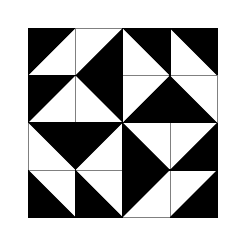
\begin{tikzpicture}[scale=0.6]
 \draw [step=1cm,gray,very thin](0,-1) grid (4,3); 
 \draw[opacity=1,fill=black](1,-1)--(0,-1)--(0,0); 
 \draw[opacity=1,fill=black](0,1)--(1,1)--(1,0); 
 \draw[opacity=1,fill=black](0,1)--(0,2)--(1,2); 
 \draw[opacity=1,fill=black](0,2)--(0,3)--(1,3); 
 \draw[opacity=1,fill=black](2,-1)--(1,-1)--(1,0); 
 \draw[opacity=1,fill=black](1,0)--(1,1)--(2,1); 
 \draw[opacity=1,fill=black](1,2)--(2,2)--(2,1); 
 \draw[opacity=1,fill=black](2,3)--(2,2)--(1,2); 
 \draw[opacity=1,fill=black](2,-1)--(2,0)--(3,0); 
 \draw[opacity=1,fill=black](3,0)--(2,0)--(2,1); 
 \draw[opacity=1,fill=black](3,2)--(3,1)--(2,1); 
 \draw[opacity=1,fill=black](2,3)--(3,3)--(3,2); 
 \draw[opacity=1,fill=black](4,0)--(4,-1)--(3,-1); 
 \draw[opacity=1,fill=black](4,1)--(4,0)--(3,0); 
 \draw[opacity=1,fill=black](4,1)--(3,1)--(3,2); 
 \draw[opacity=1,fill=black](3,3)--(4,3)--(4,2); 
\end{tikzpicture} 
\\ 
 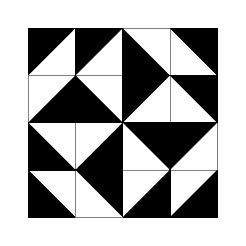
\begin{tikzpicture}[scale=0.6]
 \draw [step=1cm,gray,very thin](0,-1) grid (4,3); 
 \draw[opacity=1,fill=black](1,-1)--(0,-1)--(0,0); 
 \draw[opacity=1,fill=black](1,0)--(0,0)--(0,1); 
 \draw[opacity=1,fill=black](1,2)--(1,1)--(0,1); 
 \draw[opacity=1,fill=black](0,2)--(0,3)--(1,3); 
 \draw[opacity=1,fill=black](1,0)--(2,0)--(2,-1); 
 \draw[opacity=1,fill=black](2,1)--(2,0)--(1,0); 
 \draw[opacity=1,fill=black](2,1)--(1,1)--(1,2); 
 \draw[opacity=1,fill=black](1,2)--(1,3)--(2,3); 
 \draw[opacity=1,fill=black](3,0)--(3,-1)--(2,-1); 
 \draw[opacity=1,fill=black](2,1)--(3,1)--(3,0); 
 \draw[opacity=1,fill=black](2,1)--(2,2)--(3,2); 
 \draw[opacity=1,fill=black](3,2)--(2,2)--(2,3); 
 \draw[opacity=1,fill=black](4,0)--(4,-1)--(3,-1); 
 \draw[opacity=1,fill=black](3,0)--(3,1)--(4,1); 
 \draw[opacity=1,fill=black](3,2)--(4,2)--(4,1); 
 \draw[opacity=1,fill=black](3,3)--(4,3)--(4,2); 
\end{tikzpicture} 
 & 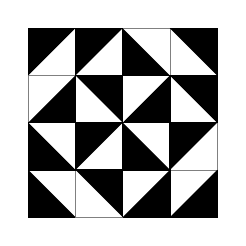
\begin{tikzpicture}[scale=0.6]
 \draw [step=1cm,gray,very thin](0,-1) grid (4,3); 
 \draw[opacity=1,fill=black](1,-1)--(0,-1)--(0,0); 
 \draw[opacity=1,fill=black](1,0)--(0,0)--(0,1); 
 \draw[opacity=1,fill=black](1,2)--(1,1)--(0,1); 
 \draw[opacity=1,fill=black](0,2)--(0,3)--(1,3); 
 \draw[opacity=1,fill=black](1,0)--(2,0)--(2,-1); 
 \draw[opacity=1,fill=black](1,0)--(1,1)--(2,1); 
 \draw[opacity=1,fill=black](1,2)--(2,2)--(2,1); 
 \draw[opacity=1,fill=black](1,2)--(1,3)--(2,3); 
 \draw[opacity=1,fill=black](3,0)--(3,-1)--(2,-1); 
 \draw[opacity=1,fill=black](3,0)--(2,0)--(2,1); 
 \draw[opacity=1,fill=black](3,2)--(3,1)--(2,1); 
 \draw[opacity=1,fill=black](3,2)--(2,2)--(2,3); 
 \draw[opacity=1,fill=black](4,0)--(4,-1)--(3,-1); 
 \draw[opacity=1,fill=black](3,0)--(3,1)--(4,1); 
 \draw[opacity=1,fill=black](3,2)--(4,2)--(4,1); 
 \draw[opacity=1,fill=black](3,3)--(4,3)--(4,2); 
\end{tikzpicture} 
 & 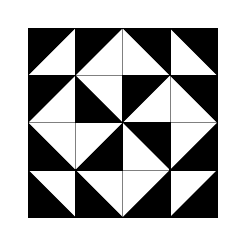
\begin{tikzpicture}[scale=0.6]
 \draw [step=1cm,gray,very thin](0,-1) grid (4,3); 
 \draw[opacity=1,fill=black](1,-1)--(0,-1)--(0,0); 
 \draw[opacity=1,fill=black](1,0)--(0,0)--(0,1); 
 \draw[opacity=1,fill=black](0,1)--(0,2)--(1,2); 
 \draw[opacity=1,fill=black](0,2)--(0,3)--(1,3); 
 \draw[opacity=1,fill=black](2,-1)--(1,-1)--(1,0); 
 \draw[opacity=1,fill=black](2,1)--(2,0)--(1,0); 
 \draw[opacity=1,fill=black](2,1)--(1,1)--(1,2); 
 \draw[opacity=1,fill=black](1,2)--(1,3)--(2,3); 
 \draw[opacity=1,fill=black](3,0)--(3,-1)--(2,-1); 
 \draw[opacity=1,fill=black](2,1)--(3,1)--(3,0); 
 \draw[opacity=1,fill=black](2,1)--(2,2)--(3,2); 
 \draw[opacity=1,fill=black](2,3)--(3,3)--(3,2); 
 \draw[opacity=1,fill=black](4,0)--(4,-1)--(3,-1); 
 \draw[opacity=1,fill=black](4,1)--(4,0)--(3,0); 
 \draw[opacity=1,fill=black](3,2)--(4,2)--(4,1); 
 \draw[opacity=1,fill=black](3,3)--(4,3)--(4,2); 
\end{tikzpicture} 
 & 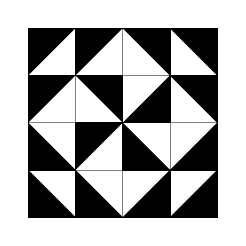
\begin{tikzpicture}[scale=0.6]
 \draw [step=1cm,gray,very thin](0,-1) grid (4,3); 
 \draw[opacity=1,fill=black](1,-1)--(0,-1)--(0,0); 
 \draw[opacity=1,fill=black](1,0)--(0,0)--(0,1); 
 \draw[opacity=1,fill=black](0,1)--(0,2)--(1,2); 
 \draw[opacity=1,fill=black](0,2)--(0,3)--(1,3); 
 \draw[opacity=1,fill=black](2,-1)--(1,-1)--(1,0); 
 \draw[opacity=1,fill=black](1,0)--(1,1)--(2,1); 
 \draw[opacity=1,fill=black](1,2)--(2,2)--(2,1); 
 \draw[opacity=1,fill=black](1,2)--(1,3)--(2,3); 
 \draw[opacity=1,fill=black](3,0)--(3,-1)--(2,-1); 
 \draw[opacity=1,fill=black](3,0)--(2,0)--(2,1); 
 \draw[opacity=1,fill=black](3,2)--(3,1)--(2,1); 
 \draw[opacity=1,fill=black](2,3)--(3,3)--(3,2); 
 \draw[opacity=1,fill=black](4,0)--(4,-1)--(3,-1); 
 \draw[opacity=1,fill=black](4,1)--(4,0)--(3,0); 
 \draw[opacity=1,fill=black](3,2)--(4,2)--(4,1); 
 \draw[opacity=1,fill=black](3,3)--(4,3)--(4,2); 
\end{tikzpicture} 
\\ 
 \end{tabular} 
\,\newline
\vspace{1cm}
{\Large
\begin{tabular}{cccc} 
0001 & 0003 & 0021 & 0023\\ 
 0201 & 0203 & 0221 & 0223\\ 
 2001 & 2003 & 2021 & 2023\\ 
 2201 & 2203 & 2221 & 2223\\ 
 \end{tabular} 
}
\,\newline
\vspace{1cm}
\begin{tabular}{cccc} 
\begin{tikzpicture}[scale=1]
 \draw [step=1cm,gray,very thin](0,-1) grid (1,0); 
 \draw[opacity=1,fill=black](0,-1)--(0,0)--(1,0); 
\end{tikzpicture} 
 & \begin{tikzpicture}[scale=1]
 \draw [step=1cm,gray,very thin](0,-1) grid (1,0); 
 \draw[opacity=1,fill=black](1,-1)--(0,-1)--(0,0); 
\end{tikzpicture} 
 & \begin{tikzpicture}[scale=1]
 \draw [step=1cm,gray,very thin](0,-1) grid (1,0); 
 \draw[opacity=1,fill=black](1,0)--(1,-1)--(0,-1); 
\end{tikzpicture} 
 & \begin{tikzpicture}[scale=1]
 \draw [step=1cm,gray,very thin](0,-1) grid (1,0); 
 \draw[opacity=1,fill=black](0,0)--(1,0)--(1,-1); 
\end{tikzpicture} 
\\ 
 \end{tabular} 
\end{center}

\newpage



\section{0010}

\vspace{1cm}
\begin{center}
\begin{tabular}{cccc} 
\begin{tikzpicture}[scale=0.6]
 \draw [step=1cm,gray,very thin](0,-1) grid (4,3); 
 \draw[opacity=1,fill=black](0,0)--(1,0)--(1,-1); 
 \draw[opacity=1,fill=black](0,1)--(1,1)--(1,0); 
 \draw[opacity=1,fill=black](1,1)--(0,1)--(0,2); 
 \draw[opacity=1,fill=black](1,3)--(1,2)--(0,2); 
 \draw[opacity=1,fill=black](2,0)--(2,-1)--(1,-1); 
 \draw[opacity=1,fill=black](1,1)--(2,1)--(2,0); 
 \draw[opacity=1,fill=black](2,2)--(2,1)--(1,1); 
 \draw[opacity=1,fill=black](2,3)--(2,2)--(1,2); 
 \draw[opacity=1,fill=black](2,-1)--(2,0)--(3,0); 
 \draw[opacity=1,fill=black](2,0)--(2,1)--(3,1); 
 \draw[opacity=1,fill=black](3,1)--(2,1)--(2,2); 
 \draw[opacity=1,fill=black](2,2)--(2,3)--(3,3); 
 \draw[opacity=1,fill=black](3,-1)--(3,0)--(4,0); 
 \draw[opacity=1,fill=black](3,1)--(4,1)--(4,0); 
 \draw[opacity=1,fill=black](4,1)--(3,1)--(3,2); 
 \draw[opacity=1,fill=black](4,2)--(3,2)--(3,3); 
\end{tikzpicture} 
 & \begin{tikzpicture}[scale=0.6]
 \draw [step=1cm,gray,very thin](0,-1) grid (4,3); 
 \draw[opacity=1,fill=black](0,0)--(1,0)--(1,-1); 
 \draw[opacity=1,fill=black](0,1)--(1,1)--(1,0); 
 \draw[opacity=1,fill=black](1,1)--(0,1)--(0,2); 
 \draw[opacity=1,fill=black](1,3)--(1,2)--(0,2); 
 \draw[opacity=1,fill=black](2,0)--(2,-1)--(1,-1); 
 \draw[opacity=1,fill=black](2,0)--(1,0)--(1,1); 
 \draw[opacity=1,fill=black](1,1)--(1,2)--(2,2); 
 \draw[opacity=1,fill=black](2,3)--(2,2)--(1,2); 
 \draw[opacity=1,fill=black](2,-1)--(2,0)--(3,0); 
 \draw[opacity=1,fill=black](3,1)--(3,0)--(2,0); 
 \draw[opacity=1,fill=black](2,2)--(3,2)--(3,1); 
 \draw[opacity=1,fill=black](2,2)--(2,3)--(3,3); 
 \draw[opacity=1,fill=black](3,-1)--(3,0)--(4,0); 
 \draw[opacity=1,fill=black](3,1)--(4,1)--(4,0); 
 \draw[opacity=1,fill=black](4,1)--(3,1)--(3,2); 
 \draw[opacity=1,fill=black](4,2)--(3,2)--(3,3); 
\end{tikzpicture} 
 & \begin{tikzpicture}[scale=0.6]
 \draw [step=1cm,gray,very thin](0,-1) grid (4,3); 
 \draw[opacity=1,fill=black](0,0)--(1,0)--(1,-1); 
 \draw[opacity=1,fill=black](0,1)--(1,1)--(1,0); 
 \draw[opacity=1,fill=black](0,2)--(1,2)--(1,1); 
 \draw[opacity=1,fill=black](1,3)--(1,2)--(0,2); 
 \draw[opacity=1,fill=black](1,-1)--(1,0)--(2,0); 
 \draw[opacity=1,fill=black](1,1)--(2,1)--(2,0); 
 \draw[opacity=1,fill=black](2,2)--(2,1)--(1,1); 
 \draw[opacity=1,fill=black](2,3)--(2,2)--(1,2); 
 \draw[opacity=1,fill=black](2,-1)--(2,0)--(3,0); 
 \draw[opacity=1,fill=black](2,0)--(2,1)--(3,1); 
 \draw[opacity=1,fill=black](3,1)--(2,1)--(2,2); 
 \draw[opacity=1,fill=black](3,3)--(3,2)--(2,2); 
 \draw[opacity=1,fill=black](3,-1)--(3,0)--(4,0); 
 \draw[opacity=1,fill=black](4,0)--(3,0)--(3,1); 
 \draw[opacity=1,fill=black](4,1)--(3,1)--(3,2); 
 \draw[opacity=1,fill=black](4,2)--(3,2)--(3,3); 
\end{tikzpicture} 
 & \begin{tikzpicture}[scale=0.6]
 \draw [step=1cm,gray,very thin](0,-1) grid (4,3); 
 \draw[opacity=1,fill=black](0,0)--(1,0)--(1,-1); 
 \draw[opacity=1,fill=black](0,1)--(1,1)--(1,0); 
 \draw[opacity=1,fill=black](0,2)--(1,2)--(1,1); 
 \draw[opacity=1,fill=black](1,3)--(1,2)--(0,2); 
 \draw[opacity=1,fill=black](1,-1)--(1,0)--(2,0); 
 \draw[opacity=1,fill=black](2,0)--(1,0)--(1,1); 
 \draw[opacity=1,fill=black](1,1)--(1,2)--(2,2); 
 \draw[opacity=1,fill=black](2,3)--(2,2)--(1,2); 
 \draw[opacity=1,fill=black](2,-1)--(2,0)--(3,0); 
 \draw[opacity=1,fill=black](3,1)--(3,0)--(2,0); 
 \draw[opacity=1,fill=black](2,2)--(3,2)--(3,1); 
 \draw[opacity=1,fill=black](3,3)--(3,2)--(2,2); 
 \draw[opacity=1,fill=black](3,-1)--(3,0)--(4,0); 
 \draw[opacity=1,fill=black](4,0)--(3,0)--(3,1); 
 \draw[opacity=1,fill=black](4,1)--(3,1)--(3,2); 
 \draw[opacity=1,fill=black](4,2)--(3,2)--(3,3); 
\end{tikzpicture} 
\\ 
 \begin{tikzpicture}[scale=0.6]
 \draw [step=1cm,gray,very thin](0,-1) grid (4,3); 
 \draw[opacity=1,fill=black](0,0)--(1,0)--(1,-1); 
 \draw[opacity=1,fill=black](1,0)--(0,0)--(0,1); 
 \draw[opacity=1,fill=black](1,1)--(0,1)--(0,2); 
 \draw[opacity=1,fill=black](1,3)--(1,2)--(0,2); 
 \draw[opacity=1,fill=black](2,0)--(2,-1)--(1,-1); 
 \draw[opacity=1,fill=black](1,1)--(2,1)--(2,0); 
 \draw[opacity=1,fill=black](2,2)--(2,1)--(1,1); 
 \draw[opacity=1,fill=black](1,2)--(1,3)--(2,3); 
 \draw[opacity=1,fill=black](3,0)--(3,-1)--(2,-1); 
 \draw[opacity=1,fill=black](2,0)--(2,1)--(3,1); 
 \draw[opacity=1,fill=black](3,1)--(2,1)--(2,2); 
 \draw[opacity=1,fill=black](2,2)--(2,3)--(3,3); 
 \draw[opacity=1,fill=black](3,-1)--(3,0)--(4,0); 
 \draw[opacity=1,fill=black](3,1)--(4,1)--(4,0); 
 \draw[opacity=1,fill=black](3,2)--(4,2)--(4,1); 
 \draw[opacity=1,fill=black](4,2)--(3,2)--(3,3); 
\end{tikzpicture} 
 & \begin{tikzpicture}[scale=0.6]
 \draw [step=1cm,gray,very thin](0,-1) grid (4,3); 
 \draw[opacity=1,fill=black](0,0)--(1,0)--(1,-1); 
 \draw[opacity=1,fill=black](1,0)--(0,0)--(0,1); 
 \draw[opacity=1,fill=black](1,1)--(0,1)--(0,2); 
 \draw[opacity=1,fill=black](1,3)--(1,2)--(0,2); 
 \draw[opacity=1,fill=black](2,0)--(2,-1)--(1,-1); 
 \draw[opacity=1,fill=black](2,0)--(1,0)--(1,1); 
 \draw[opacity=1,fill=black](1,1)--(1,2)--(2,2); 
 \draw[opacity=1,fill=black](1,2)--(1,3)--(2,3); 
 \draw[opacity=1,fill=black](3,0)--(3,-1)--(2,-1); 
 \draw[opacity=1,fill=black](3,1)--(3,0)--(2,0); 
 \draw[opacity=1,fill=black](2,2)--(3,2)--(3,1); 
 \draw[opacity=1,fill=black](2,2)--(2,3)--(3,3); 
 \draw[opacity=1,fill=black](3,-1)--(3,0)--(4,0); 
 \draw[opacity=1,fill=black](3,1)--(4,1)--(4,0); 
 \draw[opacity=1,fill=black](3,2)--(4,2)--(4,1); 
 \draw[opacity=1,fill=black](4,2)--(3,2)--(3,3); 
\end{tikzpicture} 
 & \begin{tikzpicture}[scale=0.6]
 \draw [step=1cm,gray,very thin](0,-1) grid (4,3); 
 \draw[opacity=1,fill=black](0,0)--(1,0)--(1,-1); 
 \draw[opacity=1,fill=black](1,0)--(0,0)--(0,1); 
 \draw[opacity=1,fill=black](0,2)--(1,2)--(1,1); 
 \draw[opacity=1,fill=black](1,3)--(1,2)--(0,2); 
 \draw[opacity=1,fill=black](1,-1)--(1,0)--(2,0); 
 \draw[opacity=1,fill=black](1,1)--(2,1)--(2,0); 
 \draw[opacity=1,fill=black](2,2)--(2,1)--(1,1); 
 \draw[opacity=1,fill=black](1,2)--(1,3)--(2,3); 
 \draw[opacity=1,fill=black](3,0)--(3,-1)--(2,-1); 
 \draw[opacity=1,fill=black](2,0)--(2,1)--(3,1); 
 \draw[opacity=1,fill=black](3,1)--(2,1)--(2,2); 
 \draw[opacity=1,fill=black](3,3)--(3,2)--(2,2); 
 \draw[opacity=1,fill=black](3,-1)--(3,0)--(4,0); 
 \draw[opacity=1,fill=black](4,0)--(3,0)--(3,1); 
 \draw[opacity=1,fill=black](3,2)--(4,2)--(4,1); 
 \draw[opacity=1,fill=black](4,2)--(3,2)--(3,3); 
\end{tikzpicture} 
 & \begin{tikzpicture}[scale=0.6]
 \draw [step=1cm,gray,very thin](0,-1) grid (4,3); 
 \draw[opacity=1,fill=black](0,0)--(1,0)--(1,-1); 
 \draw[opacity=1,fill=black](1,0)--(0,0)--(0,1); 
 \draw[opacity=1,fill=black](0,2)--(1,2)--(1,1); 
 \draw[opacity=1,fill=black](1,3)--(1,2)--(0,2); 
 \draw[opacity=1,fill=black](1,-1)--(1,0)--(2,0); 
 \draw[opacity=1,fill=black](2,0)--(1,0)--(1,1); 
 \draw[opacity=1,fill=black](1,1)--(1,2)--(2,2); 
 \draw[opacity=1,fill=black](1,2)--(1,3)--(2,3); 
 \draw[opacity=1,fill=black](3,0)--(3,-1)--(2,-1); 
 \draw[opacity=1,fill=black](3,1)--(3,0)--(2,0); 
 \draw[opacity=1,fill=black](2,2)--(3,2)--(3,1); 
 \draw[opacity=1,fill=black](3,3)--(3,2)--(2,2); 
 \draw[opacity=1,fill=black](3,-1)--(3,0)--(4,0); 
 \draw[opacity=1,fill=black](4,0)--(3,0)--(3,1); 
 \draw[opacity=1,fill=black](3,2)--(4,2)--(4,1); 
 \draw[opacity=1,fill=black](4,2)--(3,2)--(3,3); 
\end{tikzpicture} 
\\ 
 \begin{tikzpicture}[scale=0.6]
 \draw [step=1cm,gray,very thin](0,-1) grid (4,3); 
 \draw[opacity=1,fill=black](1,-1)--(0,-1)--(0,0); 
 \draw[opacity=1,fill=black](0,1)--(1,1)--(1,0); 
 \draw[opacity=1,fill=black](1,1)--(0,1)--(0,2); 
 \draw[opacity=1,fill=black](0,2)--(0,3)--(1,3); 
 \draw[opacity=1,fill=black](2,0)--(2,-1)--(1,-1); 
 \draw[opacity=1,fill=black](1,1)--(2,1)--(2,0); 
 \draw[opacity=1,fill=black](2,2)--(2,1)--(1,1); 
 \draw[opacity=1,fill=black](2,3)--(2,2)--(1,2); 
 \draw[opacity=1,fill=black](2,-1)--(2,0)--(3,0); 
 \draw[opacity=1,fill=black](2,0)--(2,1)--(3,1); 
 \draw[opacity=1,fill=black](3,1)--(2,1)--(2,2); 
 \draw[opacity=1,fill=black](2,2)--(2,3)--(3,3); 
 \draw[opacity=1,fill=black](4,0)--(4,-1)--(3,-1); 
 \draw[opacity=1,fill=black](3,1)--(4,1)--(4,0); 
 \draw[opacity=1,fill=black](4,1)--(3,1)--(3,2); 
 \draw[opacity=1,fill=black](3,3)--(4,3)--(4,2); 
\end{tikzpicture} 
 & \begin{tikzpicture}[scale=0.6]
 \draw [step=1cm,gray,very thin](0,-1) grid (4,3); 
 \draw[opacity=1,fill=black](1,-1)--(0,-1)--(0,0); 
 \draw[opacity=1,fill=black](0,1)--(1,1)--(1,0); 
 \draw[opacity=1,fill=black](1,1)--(0,1)--(0,2); 
 \draw[opacity=1,fill=black](0,2)--(0,3)--(1,3); 
 \draw[opacity=1,fill=black](2,0)--(2,-1)--(1,-1); 
 \draw[opacity=1,fill=black](2,0)--(1,0)--(1,1); 
 \draw[opacity=1,fill=black](1,1)--(1,2)--(2,2); 
 \draw[opacity=1,fill=black](2,3)--(2,2)--(1,2); 
 \draw[opacity=1,fill=black](2,-1)--(2,0)--(3,0); 
 \draw[opacity=1,fill=black](3,1)--(3,0)--(2,0); 
 \draw[opacity=1,fill=black](2,2)--(3,2)--(3,1); 
 \draw[opacity=1,fill=black](2,2)--(2,3)--(3,3); 
 \draw[opacity=1,fill=black](4,0)--(4,-1)--(3,-1); 
 \draw[opacity=1,fill=black](3,1)--(4,1)--(4,0); 
 \draw[opacity=1,fill=black](4,1)--(3,1)--(3,2); 
 \draw[opacity=1,fill=black](3,3)--(4,3)--(4,2); 
\end{tikzpicture} 
 & \begin{tikzpicture}[scale=0.6]
 \draw [step=1cm,gray,very thin](0,-1) grid (4,3); 
 \draw[opacity=1,fill=black](1,-1)--(0,-1)--(0,0); 
 \draw[opacity=1,fill=black](0,1)--(1,1)--(1,0); 
 \draw[opacity=1,fill=black](0,2)--(1,2)--(1,1); 
 \draw[opacity=1,fill=black](0,2)--(0,3)--(1,3); 
 \draw[opacity=1,fill=black](1,-1)--(1,0)--(2,0); 
 \draw[opacity=1,fill=black](1,1)--(2,1)--(2,0); 
 \draw[opacity=1,fill=black](2,2)--(2,1)--(1,1); 
 \draw[opacity=1,fill=black](2,3)--(2,2)--(1,2); 
 \draw[opacity=1,fill=black](2,-1)--(2,0)--(3,0); 
 \draw[opacity=1,fill=black](2,0)--(2,1)--(3,1); 
 \draw[opacity=1,fill=black](3,1)--(2,1)--(2,2); 
 \draw[opacity=1,fill=black](3,3)--(3,2)--(2,2); 
 \draw[opacity=1,fill=black](4,0)--(4,-1)--(3,-1); 
 \draw[opacity=1,fill=black](4,0)--(3,0)--(3,1); 
 \draw[opacity=1,fill=black](4,1)--(3,1)--(3,2); 
 \draw[opacity=1,fill=black](3,3)--(4,3)--(4,2); 
\end{tikzpicture} 
 & \begin{tikzpicture}[scale=0.6]
 \draw [step=1cm,gray,very thin](0,-1) grid (4,3); 
 \draw[opacity=1,fill=black](1,-1)--(0,-1)--(0,0); 
 \draw[opacity=1,fill=black](0,1)--(1,1)--(1,0); 
 \draw[opacity=1,fill=black](0,2)--(1,2)--(1,1); 
 \draw[opacity=1,fill=black](0,2)--(0,3)--(1,3); 
 \draw[opacity=1,fill=black](1,-1)--(1,0)--(2,0); 
 \draw[opacity=1,fill=black](2,0)--(1,0)--(1,1); 
 \draw[opacity=1,fill=black](1,1)--(1,2)--(2,2); 
 \draw[opacity=1,fill=black](2,3)--(2,2)--(1,2); 
 \draw[opacity=1,fill=black](2,-1)--(2,0)--(3,0); 
 \draw[opacity=1,fill=black](3,1)--(3,0)--(2,0); 
 \draw[opacity=1,fill=black](2,2)--(3,2)--(3,1); 
 \draw[opacity=1,fill=black](3,3)--(3,2)--(2,2); 
 \draw[opacity=1,fill=black](4,0)--(4,-1)--(3,-1); 
 \draw[opacity=1,fill=black](4,0)--(3,0)--(3,1); 
 \draw[opacity=1,fill=black](4,1)--(3,1)--(3,2); 
 \draw[opacity=1,fill=black](3,3)--(4,3)--(4,2); 
\end{tikzpicture} 
\\ 
 \begin{tikzpicture}[scale=0.6]
 \draw [step=1cm,gray,very thin](0,-1) grid (4,3); 
 \draw[opacity=1,fill=black](1,-1)--(0,-1)--(0,0); 
 \draw[opacity=1,fill=black](1,0)--(0,0)--(0,1); 
 \draw[opacity=1,fill=black](1,1)--(0,1)--(0,2); 
 \draw[opacity=1,fill=black](0,2)--(0,3)--(1,3); 
 \draw[opacity=1,fill=black](2,0)--(2,-1)--(1,-1); 
 \draw[opacity=1,fill=black](1,1)--(2,1)--(2,0); 
 \draw[opacity=1,fill=black](2,2)--(2,1)--(1,1); 
 \draw[opacity=1,fill=black](1,2)--(1,3)--(2,3); 
 \draw[opacity=1,fill=black](3,0)--(3,-1)--(2,-1); 
 \draw[opacity=1,fill=black](2,0)--(2,1)--(3,1); 
 \draw[opacity=1,fill=black](3,1)--(2,1)--(2,2); 
 \draw[opacity=1,fill=black](2,2)--(2,3)--(3,3); 
 \draw[opacity=1,fill=black](4,0)--(4,-1)--(3,-1); 
 \draw[opacity=1,fill=black](3,1)--(4,1)--(4,0); 
 \draw[opacity=1,fill=black](3,2)--(4,2)--(4,1); 
 \draw[opacity=1,fill=black](3,3)--(4,3)--(4,2); 
\end{tikzpicture} 
 & \begin{tikzpicture}[scale=0.6]
 \draw [step=1cm,gray,very thin](0,-1) grid (4,3); 
 \draw[opacity=1,fill=black](1,-1)--(0,-1)--(0,0); 
 \draw[opacity=1,fill=black](1,0)--(0,0)--(0,1); 
 \draw[opacity=1,fill=black](1,1)--(0,1)--(0,2); 
 \draw[opacity=1,fill=black](0,2)--(0,3)--(1,3); 
 \draw[opacity=1,fill=black](2,0)--(2,-1)--(1,-1); 
 \draw[opacity=1,fill=black](2,0)--(1,0)--(1,1); 
 \draw[opacity=1,fill=black](1,1)--(1,2)--(2,2); 
 \draw[opacity=1,fill=black](1,2)--(1,3)--(2,3); 
 \draw[opacity=1,fill=black](3,0)--(3,-1)--(2,-1); 
 \draw[opacity=1,fill=black](3,1)--(3,0)--(2,0); 
 \draw[opacity=1,fill=black](2,2)--(3,2)--(3,1); 
 \draw[opacity=1,fill=black](2,2)--(2,3)--(3,3); 
 \draw[opacity=1,fill=black](4,0)--(4,-1)--(3,-1); 
 \draw[opacity=1,fill=black](3,1)--(4,1)--(4,0); 
 \draw[opacity=1,fill=black](3,2)--(4,2)--(4,1); 
 \draw[opacity=1,fill=black](3,3)--(4,3)--(4,2); 
\end{tikzpicture} 
 & \begin{tikzpicture}[scale=0.6]
 \draw [step=1cm,gray,very thin](0,-1) grid (4,3); 
 \draw[opacity=1,fill=black](1,-1)--(0,-1)--(0,0); 
 \draw[opacity=1,fill=black](1,0)--(0,0)--(0,1); 
 \draw[opacity=1,fill=black](0,2)--(1,2)--(1,1); 
 \draw[opacity=1,fill=black](0,2)--(0,3)--(1,3); 
 \draw[opacity=1,fill=black](1,-1)--(1,0)--(2,0); 
 \draw[opacity=1,fill=black](1,1)--(2,1)--(2,0); 
 \draw[opacity=1,fill=black](2,2)--(2,1)--(1,1); 
 \draw[opacity=1,fill=black](1,2)--(1,3)--(2,3); 
 \draw[opacity=1,fill=black](3,0)--(3,-1)--(2,-1); 
 \draw[opacity=1,fill=black](2,0)--(2,1)--(3,1); 
 \draw[opacity=1,fill=black](3,1)--(2,1)--(2,2); 
 \draw[opacity=1,fill=black](3,3)--(3,2)--(2,2); 
 \draw[opacity=1,fill=black](4,0)--(4,-1)--(3,-1); 
 \draw[opacity=1,fill=black](4,0)--(3,0)--(3,1); 
 \draw[opacity=1,fill=black](3,2)--(4,2)--(4,1); 
 \draw[opacity=1,fill=black](3,3)--(4,3)--(4,2); 
\end{tikzpicture} 
 & \begin{tikzpicture}[scale=0.6]
 \draw [step=1cm,gray,very thin](0,-1) grid (4,3); 
 \draw[opacity=1,fill=black](1,-1)--(0,-1)--(0,0); 
 \draw[opacity=1,fill=black](1,0)--(0,0)--(0,1); 
 \draw[opacity=1,fill=black](0,2)--(1,2)--(1,1); 
 \draw[opacity=1,fill=black](0,2)--(0,3)--(1,3); 
 \draw[opacity=1,fill=black](1,-1)--(1,0)--(2,0); 
 \draw[opacity=1,fill=black](2,0)--(1,0)--(1,1); 
 \draw[opacity=1,fill=black](1,1)--(1,2)--(2,2); 
 \draw[opacity=1,fill=black](1,2)--(1,3)--(2,3); 
 \draw[opacity=1,fill=black](3,0)--(3,-1)--(2,-1); 
 \draw[opacity=1,fill=black](3,1)--(3,0)--(2,0); 
 \draw[opacity=1,fill=black](2,2)--(3,2)--(3,1); 
 \draw[opacity=1,fill=black](3,3)--(3,2)--(2,2); 
 \draw[opacity=1,fill=black](4,0)--(4,-1)--(3,-1); 
 \draw[opacity=1,fill=black](4,0)--(3,0)--(3,1); 
 \draw[opacity=1,fill=black](3,2)--(4,2)--(4,1); 
 \draw[opacity=1,fill=black](3,3)--(4,3)--(4,2); 
\end{tikzpicture} 
\\ 
 \end{tabular} 
{\Large
\vspace{1cm}\begin{tabular}{cccc} 
0010 & 0012 & 0030 & 0032\\ 
 0210 & 0212 & 0230 & 0232\\ 
 2010 & 2012 & 2030 & 2032\\ 
 2210 & 2212 & 2230 & 2232\\ 
 \end{tabular} 
}
\end{center}

\newpage



\section{0011}

\begin{center}
\begin{tabular}{cccc} 
\begin{tikzpicture}[scale=0.75]
 \draw [step=1cm,gray,very thin](0,-1) grid (4,3); 
 \draw[opacity=1,fill=black](0,0)--(1,0)--(1,-1); 
 \draw[opacity=1,fill=black](0,1)--(1,1)--(1,0); 
 \draw[opacity=1,fill=black](1,1)--(0,1)--(0,2); 
 \draw[opacity=1,fill=black](1,3)--(1,2)--(0,2); 
 \draw[opacity=1,fill=black](2,0)--(2,-1)--(1,-1); 
 \draw[opacity=1,fill=black](2,1)--(2,0)--(1,0); 
 \draw[opacity=1,fill=black](2,1)--(1,1)--(1,2); 
 \draw[opacity=1,fill=black](2,3)--(2,2)--(1,2); 
 \draw[opacity=1,fill=black](2,-1)--(2,0)--(3,0); 
 \draw[opacity=1,fill=black](2,1)--(3,1)--(3,0); 
 \draw[opacity=1,fill=black](2,1)--(2,2)--(3,2); 
 \draw[opacity=1,fill=black](2,2)--(2,3)--(3,3); 
 \draw[opacity=1,fill=black](3,-1)--(3,0)--(4,0); 
 \draw[opacity=1,fill=black](3,1)--(4,1)--(4,0); 
 \draw[opacity=1,fill=black](4,1)--(3,1)--(3,2); 
 \draw[opacity=1,fill=black](4,2)--(3,2)--(3,3); 
\end{tikzpicture} 
 & \begin{tikzpicture}[scale=0.75]
 \draw [step=1cm,gray,very thin](0,-1) grid (4,3); 
 \draw[opacity=1,fill=black](0,0)--(1,0)--(1,-1); 
 \draw[opacity=1,fill=black](0,1)--(1,1)--(1,0); 
 \draw[opacity=1,fill=black](1,1)--(0,1)--(0,2); 
 \draw[opacity=1,fill=black](1,3)--(1,2)--(0,2); 
 \draw[opacity=1,fill=black](2,0)--(2,-1)--(1,-1); 
 \draw[opacity=1,fill=black](1,0)--(1,1)--(2,1); 
 \draw[opacity=1,fill=black](1,2)--(2,2)--(2,1); 
 \draw[opacity=1,fill=black](2,3)--(2,2)--(1,2); 
 \draw[opacity=1,fill=black](2,-1)--(2,0)--(3,0); 
 \draw[opacity=1,fill=black](3,0)--(2,0)--(2,1); 
 \draw[opacity=1,fill=black](3,2)--(3,1)--(2,1); 
 \draw[opacity=1,fill=black](2,2)--(2,3)--(3,3); 
 \draw[opacity=1,fill=black](3,-1)--(3,0)--(4,0); 
 \draw[opacity=1,fill=black](3,1)--(4,1)--(4,0); 
 \draw[opacity=1,fill=black](4,1)--(3,1)--(3,2); 
 \draw[opacity=1,fill=black](4,2)--(3,2)--(3,3); 
\end{tikzpicture} 
 & \begin{tikzpicture}[scale=0.75]
 \draw [step=1cm,gray,very thin](0,-1) grid (4,3); 
 \draw[opacity=1,fill=black](0,0)--(1,0)--(1,-1); 
 \draw[opacity=1,fill=black](0,1)--(1,1)--(1,0); 
 \draw[opacity=1,fill=black](0,2)--(1,2)--(1,1); 
 \draw[opacity=1,fill=black](1,3)--(1,2)--(0,2); 
 \draw[opacity=1,fill=black](1,-1)--(1,0)--(2,0); 
 \draw[opacity=1,fill=black](2,1)--(2,0)--(1,0); 
 \draw[opacity=1,fill=black](2,1)--(1,1)--(1,2); 
 \draw[opacity=1,fill=black](2,3)--(2,2)--(1,2); 
 \draw[opacity=1,fill=black](2,-1)--(2,0)--(3,0); 
 \draw[opacity=1,fill=black](2,1)--(3,1)--(3,0); 
 \draw[opacity=1,fill=black](2,1)--(2,2)--(3,2); 
 \draw[opacity=1,fill=black](3,3)--(3,2)--(2,2); 
 \draw[opacity=1,fill=black](3,-1)--(3,0)--(4,0); 
 \draw[opacity=1,fill=black](4,0)--(3,0)--(3,1); 
 \draw[opacity=1,fill=black](4,1)--(3,1)--(3,2); 
 \draw[opacity=1,fill=black](4,2)--(3,2)--(3,3); 
\end{tikzpicture} 
 & \begin{tikzpicture}[scale=0.75]
 \draw [step=1cm,gray,very thin](0,-1) grid (4,3); 
 \draw[opacity=1,fill=black](0,0)--(1,0)--(1,-1); 
 \draw[opacity=1,fill=black](0,1)--(1,1)--(1,0); 
 \draw[opacity=1,fill=black](0,2)--(1,2)--(1,1); 
 \draw[opacity=1,fill=black](1,3)--(1,2)--(0,2); 
 \draw[opacity=1,fill=black](1,-1)--(1,0)--(2,0); 
 \draw[opacity=1,fill=black](1,0)--(1,1)--(2,1); 
 \draw[opacity=1,fill=black](1,2)--(2,2)--(2,1); 
 \draw[opacity=1,fill=black](2,3)--(2,2)--(1,2); 
 \draw[opacity=1,fill=black](2,-1)--(2,0)--(3,0); 
 \draw[opacity=1,fill=black](3,0)--(2,0)--(2,1); 
 \draw[opacity=1,fill=black](3,2)--(3,1)--(2,1); 
 \draw[opacity=1,fill=black](3,3)--(3,2)--(2,2); 
 \draw[opacity=1,fill=black](3,-1)--(3,0)--(4,0); 
 \draw[opacity=1,fill=black](4,0)--(3,0)--(3,1); 
 \draw[opacity=1,fill=black](4,1)--(3,1)--(3,2); 
 \draw[opacity=1,fill=black](4,2)--(3,2)--(3,3); 
\end{tikzpicture} 
\\ 
 \begin{tikzpicture}[scale=0.75]
 \draw [step=1cm,gray,very thin](0,-1) grid (4,3); 
 \draw[opacity=1,fill=black](0,0)--(1,0)--(1,-1); 
 \draw[opacity=1,fill=black](1,0)--(0,0)--(0,1); 
 \draw[opacity=1,fill=black](1,1)--(0,1)--(0,2); 
 \draw[opacity=1,fill=black](1,3)--(1,2)--(0,2); 
 \draw[opacity=1,fill=black](2,0)--(2,-1)--(1,-1); 
 \draw[opacity=1,fill=black](2,1)--(2,0)--(1,0); 
 \draw[opacity=1,fill=black](2,1)--(1,1)--(1,2); 
 \draw[opacity=1,fill=black](1,2)--(1,3)--(2,3); 
 \draw[opacity=1,fill=black](3,0)--(3,-1)--(2,-1); 
 \draw[opacity=1,fill=black](2,1)--(3,1)--(3,0); 
 \draw[opacity=1,fill=black](2,1)--(2,2)--(3,2); 
 \draw[opacity=1,fill=black](2,2)--(2,3)--(3,3); 
 \draw[opacity=1,fill=black](3,-1)--(3,0)--(4,0); 
 \draw[opacity=1,fill=black](3,1)--(4,1)--(4,0); 
 \draw[opacity=1,fill=black](3,2)--(4,2)--(4,1); 
 \draw[opacity=1,fill=black](4,2)--(3,2)--(3,3); 
\end{tikzpicture} 
 & \begin{tikzpicture}[scale=0.75]
 \draw [step=1cm,gray,very thin](0,-1) grid (4,3); 
 \draw[opacity=1,fill=black](0,0)--(1,0)--(1,-1); 
 \draw[opacity=1,fill=black](1,0)--(0,0)--(0,1); 
 \draw[opacity=1,fill=black](1,1)--(0,1)--(0,2); 
 \draw[opacity=1,fill=black](1,3)--(1,2)--(0,2); 
 \draw[opacity=1,fill=black](2,0)--(2,-1)--(1,-1); 
 \draw[opacity=1,fill=black](1,0)--(1,1)--(2,1); 
 \draw[opacity=1,fill=black](1,2)--(2,2)--(2,1); 
 \draw[opacity=1,fill=black](1,2)--(1,3)--(2,3); 
 \draw[opacity=1,fill=black](3,0)--(3,-1)--(2,-1); 
 \draw[opacity=1,fill=black](3,0)--(2,0)--(2,1); 
 \draw[opacity=1,fill=black](3,2)--(3,1)--(2,1); 
 \draw[opacity=1,fill=black](2,2)--(2,3)--(3,3); 
 \draw[opacity=1,fill=black](3,-1)--(3,0)--(4,0); 
 \draw[opacity=1,fill=black](3,1)--(4,1)--(4,0); 
 \draw[opacity=1,fill=black](3,2)--(4,2)--(4,1); 
 \draw[opacity=1,fill=black](4,2)--(3,2)--(3,3); 
\end{tikzpicture} 
 & \begin{tikzpicture}[scale=0.75]
 \draw [step=1cm,gray,very thin](0,-1) grid (4,3); 
 \draw[opacity=1,fill=black](0,0)--(1,0)--(1,-1); 
 \draw[opacity=1,fill=black](1,0)--(0,0)--(0,1); 
 \draw[opacity=1,fill=black](0,2)--(1,2)--(1,1); 
 \draw[opacity=1,fill=black](1,3)--(1,2)--(0,2); 
 \draw[opacity=1,fill=black](1,-1)--(1,0)--(2,0); 
 \draw[opacity=1,fill=black](2,1)--(2,0)--(1,0); 
 \draw[opacity=1,fill=black](2,1)--(1,1)--(1,2); 
 \draw[opacity=1,fill=black](1,2)--(1,3)--(2,3); 
 \draw[opacity=1,fill=black](3,0)--(3,-1)--(2,-1); 
 \draw[opacity=1,fill=black](2,1)--(3,1)--(3,0); 
 \draw[opacity=1,fill=black](2,1)--(2,2)--(3,2); 
 \draw[opacity=1,fill=black](3,3)--(3,2)--(2,2); 
 \draw[opacity=1,fill=black](3,-1)--(3,0)--(4,0); 
 \draw[opacity=1,fill=black](4,0)--(3,0)--(3,1); 
 \draw[opacity=1,fill=black](3,2)--(4,2)--(4,1); 
 \draw[opacity=1,fill=black](4,2)--(3,2)--(3,3); 
\end{tikzpicture} 
 & \begin{tikzpicture}[scale=0.75]
 \draw [step=1cm,gray,very thin](0,-1) grid (4,3); 
 \draw[opacity=1,fill=black](0,0)--(1,0)--(1,-1); 
 \draw[opacity=1,fill=black](1,0)--(0,0)--(0,1); 
 \draw[opacity=1,fill=black](0,2)--(1,2)--(1,1); 
 \draw[opacity=1,fill=black](1,3)--(1,2)--(0,2); 
 \draw[opacity=1,fill=black](1,-1)--(1,0)--(2,0); 
 \draw[opacity=1,fill=black](1,0)--(1,1)--(2,1); 
 \draw[opacity=1,fill=black](1,2)--(2,2)--(2,1); 
 \draw[opacity=1,fill=black](1,2)--(1,3)--(2,3); 
 \draw[opacity=1,fill=black](3,0)--(3,-1)--(2,-1); 
 \draw[opacity=1,fill=black](3,0)--(2,0)--(2,1); 
 \draw[opacity=1,fill=black](3,2)--(3,1)--(2,1); 
 \draw[opacity=1,fill=black](3,3)--(3,2)--(2,2); 
 \draw[opacity=1,fill=black](3,-1)--(3,0)--(4,0); 
 \draw[opacity=1,fill=black](4,0)--(3,0)--(3,1); 
 \draw[opacity=1,fill=black](3,2)--(4,2)--(4,1); 
 \draw[opacity=1,fill=black](4,2)--(3,2)--(3,3); 
\end{tikzpicture} 
\\ 
 \begin{tikzpicture}[scale=0.75]
 \draw [step=1cm,gray,very thin](0,-1) grid (4,3); 
 \draw[opacity=1,fill=black](1,-1)--(0,-1)--(0,0); 
 \draw[opacity=1,fill=black](0,1)--(1,1)--(1,0); 
 \draw[opacity=1,fill=black](1,1)--(0,1)--(0,2); 
 \draw[opacity=1,fill=black](0,2)--(0,3)--(1,3); 
 \draw[opacity=1,fill=black](2,0)--(2,-1)--(1,-1); 
 \draw[opacity=1,fill=black](2,1)--(2,0)--(1,0); 
 \draw[opacity=1,fill=black](2,1)--(1,1)--(1,2); 
 \draw[opacity=1,fill=black](2,3)--(2,2)--(1,2); 
 \draw[opacity=1,fill=black](2,-1)--(2,0)--(3,0); 
 \draw[opacity=1,fill=black](2,1)--(3,1)--(3,0); 
 \draw[opacity=1,fill=black](2,1)--(2,2)--(3,2); 
 \draw[opacity=1,fill=black](2,2)--(2,3)--(3,3); 
 \draw[opacity=1,fill=black](4,0)--(4,-1)--(3,-1); 
 \draw[opacity=1,fill=black](3,1)--(4,1)--(4,0); 
 \draw[opacity=1,fill=black](4,1)--(3,1)--(3,2); 
 \draw[opacity=1,fill=black](3,3)--(4,3)--(4,2); 
\end{tikzpicture} 
 & \begin{tikzpicture}[scale=0.75]
 \draw [step=1cm,gray,very thin](0,-1) grid (4,3); 
 \draw[opacity=1,fill=black](1,-1)--(0,-1)--(0,0); 
 \draw[opacity=1,fill=black](0,1)--(1,1)--(1,0); 
 \draw[opacity=1,fill=black](1,1)--(0,1)--(0,2); 
 \draw[opacity=1,fill=black](0,2)--(0,3)--(1,3); 
 \draw[opacity=1,fill=black](2,0)--(2,-1)--(1,-1); 
 \draw[opacity=1,fill=black](1,0)--(1,1)--(2,1); 
 \draw[opacity=1,fill=black](1,2)--(2,2)--(2,1); 
 \draw[opacity=1,fill=black](2,3)--(2,2)--(1,2); 
 \draw[opacity=1,fill=black](2,-1)--(2,0)--(3,0); 
 \draw[opacity=1,fill=black](3,0)--(2,0)--(2,1); 
 \draw[opacity=1,fill=black](3,2)--(3,1)--(2,1); 
 \draw[opacity=1,fill=black](2,2)--(2,3)--(3,3); 
 \draw[opacity=1,fill=black](4,0)--(4,-1)--(3,-1); 
 \draw[opacity=1,fill=black](3,1)--(4,1)--(4,0); 
 \draw[opacity=1,fill=black](4,1)--(3,1)--(3,2); 
 \draw[opacity=1,fill=black](3,3)--(4,3)--(4,2); 
\end{tikzpicture} 
 & \begin{tikzpicture}[scale=0.75]
 \draw [step=1cm,gray,very thin](0,-1) grid (4,3); 
 \draw[opacity=1,fill=black](1,-1)--(0,-1)--(0,0); 
 \draw[opacity=1,fill=black](0,1)--(1,1)--(1,0); 
 \draw[opacity=1,fill=black](0,2)--(1,2)--(1,1); 
 \draw[opacity=1,fill=black](0,2)--(0,3)--(1,3); 
 \draw[opacity=1,fill=black](1,-1)--(1,0)--(2,0); 
 \draw[opacity=1,fill=black](2,1)--(2,0)--(1,0); 
 \draw[opacity=1,fill=black](2,1)--(1,1)--(1,2); 
 \draw[opacity=1,fill=black](2,3)--(2,2)--(1,2); 
 \draw[opacity=1,fill=black](2,-1)--(2,0)--(3,0); 
 \draw[opacity=1,fill=black](2,1)--(3,1)--(3,0); 
 \draw[opacity=1,fill=black](2,1)--(2,2)--(3,2); 
 \draw[opacity=1,fill=black](3,3)--(3,2)--(2,2); 
 \draw[opacity=1,fill=black](4,0)--(4,-1)--(3,-1); 
 \draw[opacity=1,fill=black](4,0)--(3,0)--(3,1); 
 \draw[opacity=1,fill=black](4,1)--(3,1)--(3,2); 
 \draw[opacity=1,fill=black](3,3)--(4,3)--(4,2); 
\end{tikzpicture} 
 & \begin{tikzpicture}[scale=0.75]
 \draw [step=1cm,gray,very thin](0,-1) grid (4,3); 
 \draw[opacity=1,fill=black](1,-1)--(0,-1)--(0,0); 
 \draw[opacity=1,fill=black](0,1)--(1,1)--(1,0); 
 \draw[opacity=1,fill=black](0,2)--(1,2)--(1,1); 
 \draw[opacity=1,fill=black](0,2)--(0,3)--(1,3); 
 \draw[opacity=1,fill=black](1,-1)--(1,0)--(2,0); 
 \draw[opacity=1,fill=black](1,0)--(1,1)--(2,1); 
 \draw[opacity=1,fill=black](1,2)--(2,2)--(2,1); 
 \draw[opacity=1,fill=black](2,3)--(2,2)--(1,2); 
 \draw[opacity=1,fill=black](2,-1)--(2,0)--(3,0); 
 \draw[opacity=1,fill=black](3,0)--(2,0)--(2,1); 
 \draw[opacity=1,fill=black](3,2)--(3,1)--(2,1); 
 \draw[opacity=1,fill=black](3,3)--(3,2)--(2,2); 
 \draw[opacity=1,fill=black](4,0)--(4,-1)--(3,-1); 
 \draw[opacity=1,fill=black](4,0)--(3,0)--(3,1); 
 \draw[opacity=1,fill=black](4,1)--(3,1)--(3,2); 
 \draw[opacity=1,fill=black](3,3)--(4,3)--(4,2); 
\end{tikzpicture} 
\\ 
 \begin{tikzpicture}[scale=0.75]
 \draw [step=1cm,gray,very thin](0,-1) grid (4,3); 
 \draw[opacity=1,fill=black](1,-1)--(0,-1)--(0,0); 
 \draw[opacity=1,fill=black](1,0)--(0,0)--(0,1); 
 \draw[opacity=1,fill=black](1,1)--(0,1)--(0,2); 
 \draw[opacity=1,fill=black](0,2)--(0,3)--(1,3); 
 \draw[opacity=1,fill=black](2,0)--(2,-1)--(1,-1); 
 \draw[opacity=1,fill=black](2,1)--(2,0)--(1,0); 
 \draw[opacity=1,fill=black](2,1)--(1,1)--(1,2); 
 \draw[opacity=1,fill=black](1,2)--(1,3)--(2,3); 
 \draw[opacity=1,fill=black](3,0)--(3,-1)--(2,-1); 
 \draw[opacity=1,fill=black](2,1)--(3,1)--(3,0); 
 \draw[opacity=1,fill=black](2,1)--(2,2)--(3,2); 
 \draw[opacity=1,fill=black](2,2)--(2,3)--(3,3); 
 \draw[opacity=1,fill=black](4,0)--(4,-1)--(3,-1); 
 \draw[opacity=1,fill=black](3,1)--(4,1)--(4,0); 
 \draw[opacity=1,fill=black](3,2)--(4,2)--(4,1); 
 \draw[opacity=1,fill=black](3,3)--(4,3)--(4,2); 
\end{tikzpicture} 
 & \begin{tikzpicture}[scale=0.75]
 \draw [step=1cm,gray,very thin](0,-1) grid (4,3); 
 \draw[opacity=1,fill=black](1,-1)--(0,-1)--(0,0); 
 \draw[opacity=1,fill=black](1,0)--(0,0)--(0,1); 
 \draw[opacity=1,fill=black](1,1)--(0,1)--(0,2); 
 \draw[opacity=1,fill=black](0,2)--(0,3)--(1,3); 
 \draw[opacity=1,fill=black](2,0)--(2,-1)--(1,-1); 
 \draw[opacity=1,fill=black](1,0)--(1,1)--(2,1); 
 \draw[opacity=1,fill=black](1,2)--(2,2)--(2,1); 
 \draw[opacity=1,fill=black](1,2)--(1,3)--(2,3); 
 \draw[opacity=1,fill=black](3,0)--(3,-1)--(2,-1); 
 \draw[opacity=1,fill=black](3,0)--(2,0)--(2,1); 
 \draw[opacity=1,fill=black](3,2)--(3,1)--(2,1); 
 \draw[opacity=1,fill=black](2,2)--(2,3)--(3,3); 
 \draw[opacity=1,fill=black](4,0)--(4,-1)--(3,-1); 
 \draw[opacity=1,fill=black](3,1)--(4,1)--(4,0); 
 \draw[opacity=1,fill=black](3,2)--(4,2)--(4,1); 
 \draw[opacity=1,fill=black](3,3)--(4,3)--(4,2); 
\end{tikzpicture} 
 & \begin{tikzpicture}[scale=0.75]
 \draw [step=1cm,gray,very thin](0,-1) grid (4,3); 
 \draw[opacity=1,fill=black](1,-1)--(0,-1)--(0,0); 
 \draw[opacity=1,fill=black](1,0)--(0,0)--(0,1); 
 \draw[opacity=1,fill=black](0,2)--(1,2)--(1,1); 
 \draw[opacity=1,fill=black](0,2)--(0,3)--(1,3); 
 \draw[opacity=1,fill=black](1,-1)--(1,0)--(2,0); 
 \draw[opacity=1,fill=black](2,1)--(2,0)--(1,0); 
 \draw[opacity=1,fill=black](2,1)--(1,1)--(1,2); 
 \draw[opacity=1,fill=black](1,2)--(1,3)--(2,3); 
 \draw[opacity=1,fill=black](3,0)--(3,-1)--(2,-1); 
 \draw[opacity=1,fill=black](2,1)--(3,1)--(3,0); 
 \draw[opacity=1,fill=black](2,1)--(2,2)--(3,2); 
 \draw[opacity=1,fill=black](3,3)--(3,2)--(2,2); 
 \draw[opacity=1,fill=black](4,0)--(4,-1)--(3,-1); 
 \draw[opacity=1,fill=black](4,0)--(3,0)--(3,1); 
 \draw[opacity=1,fill=black](3,2)--(4,2)--(4,1); 
 \draw[opacity=1,fill=black](3,3)--(4,3)--(4,2); 
\end{tikzpicture} 
 & \begin{tikzpicture}[scale=0.75]
 \draw [step=1cm,gray,very thin](0,-1) grid (4,3); 
 \draw[opacity=1,fill=black](1,-1)--(0,-1)--(0,0); 
 \draw[opacity=1,fill=black](1,0)--(0,0)--(0,1); 
 \draw[opacity=1,fill=black](0,2)--(1,2)--(1,1); 
 \draw[opacity=1,fill=black](0,2)--(0,3)--(1,3); 
 \draw[opacity=1,fill=black](1,-1)--(1,0)--(2,0); 
 \draw[opacity=1,fill=black](1,0)--(1,1)--(2,1); 
 \draw[opacity=1,fill=black](1,2)--(2,2)--(2,1); 
 \draw[opacity=1,fill=black](1,2)--(1,3)--(2,3); 
 \draw[opacity=1,fill=black](3,0)--(3,-1)--(2,-1); 
 \draw[opacity=1,fill=black](3,0)--(2,0)--(2,1); 
 \draw[opacity=1,fill=black](3,2)--(3,1)--(2,1); 
 \draw[opacity=1,fill=black](3,3)--(3,2)--(2,2); 
 \draw[opacity=1,fill=black](4,0)--(4,-1)--(3,-1); 
 \draw[opacity=1,fill=black](4,0)--(3,0)--(3,1); 
 \draw[opacity=1,fill=black](3,2)--(4,2)--(4,1); 
 \draw[opacity=1,fill=black](3,3)--(4,3)--(4,2); 
\end{tikzpicture} 
\\ 
 \end{tabular} 
\marginnote{[object Object]}
\end{center}

\newpage



\section{0100}

\vspace{1cm}
\begin{center}
\begin{tabular}{cccc} 
\begin{tikzpicture}[scale=0.6]
 \draw [step=1cm,gray,very thin](0,-1) grid (4,3); 
 \draw[opacity=1,fill=black](0,0)--(1,0)--(1,-1); 
 \draw[opacity=1,fill=black](1,1)--(1,0)--(0,0); 
 \draw[opacity=1,fill=black](1,2)--(1,1)--(0,1); 
 \draw[opacity=1,fill=black](1,3)--(1,2)--(0,2); 
 \draw[opacity=1,fill=black](1,0)--(2,0)--(2,-1); 
 \draw[opacity=1,fill=black](1,1)--(2,1)--(2,0); 
 \draw[opacity=1,fill=black](2,2)--(2,1)--(1,1); 
 \draw[opacity=1,fill=black](2,2)--(1,2)--(1,3); 
 \draw[opacity=1,fill=black](2,0)--(3,0)--(3,-1); 
 \draw[opacity=1,fill=black](2,0)--(2,1)--(3,1); 
 \draw[opacity=1,fill=black](3,1)--(2,1)--(2,2); 
 \draw[opacity=1,fill=black](3,2)--(2,2)--(2,3); 
 \draw[opacity=1,fill=black](3,-1)--(3,0)--(4,0); 
 \draw[opacity=1,fill=black](3,0)--(3,1)--(4,1); 
 \draw[opacity=1,fill=black](3,1)--(3,2)--(4,2); 
 \draw[opacity=1,fill=black](4,2)--(3,2)--(3,3); 
\end{tikzpicture} 
 & \begin{tikzpicture}[scale=0.6]
 \draw [step=1cm,gray,very thin](0,-1) grid (4,3); 
 \draw[opacity=1,fill=black](0,0)--(1,0)--(1,-1); 
 \draw[opacity=1,fill=black](1,1)--(1,0)--(0,0); 
 \draw[opacity=1,fill=black](1,2)--(1,1)--(0,1); 
 \draw[opacity=1,fill=black](1,3)--(1,2)--(0,2); 
 \draw[opacity=1,fill=black](1,0)--(2,0)--(2,-1); 
 \draw[opacity=1,fill=black](2,0)--(1,0)--(1,1); 
 \draw[opacity=1,fill=black](1,1)--(1,2)--(2,2); 
 \draw[opacity=1,fill=black](2,2)--(1,2)--(1,3); 
 \draw[opacity=1,fill=black](2,0)--(3,0)--(3,-1); 
 \draw[opacity=1,fill=black](3,1)--(3,0)--(2,0); 
 \draw[opacity=1,fill=black](2,2)--(3,2)--(3,1); 
 \draw[opacity=1,fill=black](3,2)--(2,2)--(2,3); 
 \draw[opacity=1,fill=black](3,-1)--(3,0)--(4,0); 
 \draw[opacity=1,fill=black](3,0)--(3,1)--(4,1); 
 \draw[opacity=1,fill=black](3,1)--(3,2)--(4,2); 
 \draw[opacity=1,fill=black](4,2)--(3,2)--(3,3); 
\end{tikzpicture} 
 & \begin{tikzpicture}[scale=0.6]
 \draw [step=1cm,gray,very thin](0,-1) grid (4,3); 
 \draw[opacity=1,fill=black](0,0)--(1,0)--(1,-1); 
 \draw[opacity=1,fill=black](1,1)--(1,0)--(0,0); 
 \draw[opacity=1,fill=black](0,1)--(0,2)--(1,2); 
 \draw[opacity=1,fill=black](1,3)--(1,2)--(0,2); 
 \draw[opacity=1,fill=black](2,-1)--(1,-1)--(1,0); 
 \draw[opacity=1,fill=black](1,1)--(2,1)--(2,0); 
 \draw[opacity=1,fill=black](2,2)--(2,1)--(1,1); 
 \draw[opacity=1,fill=black](2,2)--(1,2)--(1,3); 
 \draw[opacity=1,fill=black](2,0)--(3,0)--(3,-1); 
 \draw[opacity=1,fill=black](2,0)--(2,1)--(3,1); 
 \draw[opacity=1,fill=black](3,1)--(2,1)--(2,2); 
 \draw[opacity=1,fill=black](2,3)--(3,3)--(3,2); 
 \draw[opacity=1,fill=black](3,-1)--(3,0)--(4,0); 
 \draw[opacity=1,fill=black](4,1)--(4,0)--(3,0); 
 \draw[opacity=1,fill=black](3,1)--(3,2)--(4,2); 
 \draw[opacity=1,fill=black](4,2)--(3,2)--(3,3); 
\end{tikzpicture} 
 & \begin{tikzpicture}[scale=0.6]
 \draw [step=1cm,gray,very thin](0,-1) grid (4,3); 
 \draw[opacity=1,fill=black](0,0)--(1,0)--(1,-1); 
 \draw[opacity=1,fill=black](1,1)--(1,0)--(0,0); 
 \draw[opacity=1,fill=black](0,1)--(0,2)--(1,2); 
 \draw[opacity=1,fill=black](1,3)--(1,2)--(0,2); 
 \draw[opacity=1,fill=black](2,-1)--(1,-1)--(1,0); 
 \draw[opacity=1,fill=black](2,0)--(1,0)--(1,1); 
 \draw[opacity=1,fill=black](1,1)--(1,2)--(2,2); 
 \draw[opacity=1,fill=black](2,2)--(1,2)--(1,3); 
 \draw[opacity=1,fill=black](2,0)--(3,0)--(3,-1); 
 \draw[opacity=1,fill=black](3,1)--(3,0)--(2,0); 
 \draw[opacity=1,fill=black](2,2)--(3,2)--(3,1); 
 \draw[opacity=1,fill=black](2,3)--(3,3)--(3,2); 
 \draw[opacity=1,fill=black](3,-1)--(3,0)--(4,0); 
 \draw[opacity=1,fill=black](4,1)--(4,0)--(3,0); 
 \draw[opacity=1,fill=black](3,1)--(3,2)--(4,2); 
 \draw[opacity=1,fill=black](4,2)--(3,2)--(3,3); 
\end{tikzpicture} 
\\ 
 \begin{tikzpicture}[scale=0.6]
 \draw [step=1cm,gray,very thin](0,-1) grid (4,3); 
 \draw[opacity=1,fill=black](0,0)--(1,0)--(1,-1); 
 \draw[opacity=1,fill=black](0,0)--(0,1)--(1,1); 
 \draw[opacity=1,fill=black](1,2)--(1,1)--(0,1); 
 \draw[opacity=1,fill=black](1,3)--(1,2)--(0,2); 
 \draw[opacity=1,fill=black](1,0)--(2,0)--(2,-1); 
 \draw[opacity=1,fill=black](1,1)--(2,1)--(2,0); 
 \draw[opacity=1,fill=black](2,2)--(2,1)--(1,1); 
 \draw[opacity=1,fill=black](1,3)--(2,3)--(2,2); 
 \draw[opacity=1,fill=black](3,-1)--(2,-1)--(2,0); 
 \draw[opacity=1,fill=black](2,0)--(2,1)--(3,1); 
 \draw[opacity=1,fill=black](3,1)--(2,1)--(2,2); 
 \draw[opacity=1,fill=black](3,2)--(2,2)--(2,3); 
 \draw[opacity=1,fill=black](3,-1)--(3,0)--(4,0); 
 \draw[opacity=1,fill=black](3,0)--(3,1)--(4,1); 
 \draw[opacity=1,fill=black](4,2)--(4,1)--(3,1); 
 \draw[opacity=1,fill=black](4,2)--(3,2)--(3,3); 
\end{tikzpicture} 
 & \begin{tikzpicture}[scale=0.6]
 \draw [step=1cm,gray,very thin](0,-1) grid (4,3); 
 \draw[opacity=1,fill=black](0,0)--(1,0)--(1,-1); 
 \draw[opacity=1,fill=black](0,0)--(0,1)--(1,1); 
 \draw[opacity=1,fill=black](1,2)--(1,1)--(0,1); 
 \draw[opacity=1,fill=black](1,3)--(1,2)--(0,2); 
 \draw[opacity=1,fill=black](1,0)--(2,0)--(2,-1); 
 \draw[opacity=1,fill=black](2,0)--(1,0)--(1,1); 
 \draw[opacity=1,fill=black](1,1)--(1,2)--(2,2); 
 \draw[opacity=1,fill=black](1,3)--(2,3)--(2,2); 
 \draw[opacity=1,fill=black](3,-1)--(2,-1)--(2,0); 
 \draw[opacity=1,fill=black](3,1)--(3,0)--(2,0); 
 \draw[opacity=1,fill=black](2,2)--(3,2)--(3,1); 
 \draw[opacity=1,fill=black](3,2)--(2,2)--(2,3); 
 \draw[opacity=1,fill=black](3,-1)--(3,0)--(4,0); 
 \draw[opacity=1,fill=black](3,0)--(3,1)--(4,1); 
 \draw[opacity=1,fill=black](4,2)--(4,1)--(3,1); 
 \draw[opacity=1,fill=black](4,2)--(3,2)--(3,3); 
\end{tikzpicture} 
 & \begin{tikzpicture}[scale=0.6]
 \draw [step=1cm,gray,very thin](0,-1) grid (4,3); 
 \draw[opacity=1,fill=black](0,0)--(1,0)--(1,-1); 
 \draw[opacity=1,fill=black](0,0)--(0,1)--(1,1); 
 \draw[opacity=1,fill=black](0,1)--(0,2)--(1,2); 
 \draw[opacity=1,fill=black](1,3)--(1,2)--(0,2); 
 \draw[opacity=1,fill=black](2,-1)--(1,-1)--(1,0); 
 \draw[opacity=1,fill=black](1,1)--(2,1)--(2,0); 
 \draw[opacity=1,fill=black](2,2)--(2,1)--(1,1); 
 \draw[opacity=1,fill=black](1,3)--(2,3)--(2,2); 
 \draw[opacity=1,fill=black](3,-1)--(2,-1)--(2,0); 
 \draw[opacity=1,fill=black](2,0)--(2,1)--(3,1); 
 \draw[opacity=1,fill=black](3,1)--(2,1)--(2,2); 
 \draw[opacity=1,fill=black](2,3)--(3,3)--(3,2); 
 \draw[opacity=1,fill=black](3,-1)--(3,0)--(4,0); 
 \draw[opacity=1,fill=black](4,1)--(4,0)--(3,0); 
 \draw[opacity=1,fill=black](4,2)--(4,1)--(3,1); 
 \draw[opacity=1,fill=black](4,2)--(3,2)--(3,3); 
\end{tikzpicture} 
 & \begin{tikzpicture}[scale=0.6]
 \draw [step=1cm,gray,very thin](0,-1) grid (4,3); 
 \draw[opacity=1,fill=black](0,0)--(1,0)--(1,-1); 
 \draw[opacity=1,fill=black](0,0)--(0,1)--(1,1); 
 \draw[opacity=1,fill=black](0,1)--(0,2)--(1,2); 
 \draw[opacity=1,fill=black](1,3)--(1,2)--(0,2); 
 \draw[opacity=1,fill=black](2,-1)--(1,-1)--(1,0); 
 \draw[opacity=1,fill=black](2,0)--(1,0)--(1,1); 
 \draw[opacity=1,fill=black](1,1)--(1,2)--(2,2); 
 \draw[opacity=1,fill=black](1,3)--(2,3)--(2,2); 
 \draw[opacity=1,fill=black](3,-1)--(2,-1)--(2,0); 
 \draw[opacity=1,fill=black](3,1)--(3,0)--(2,0); 
 \draw[opacity=1,fill=black](2,2)--(3,2)--(3,1); 
 \draw[opacity=1,fill=black](2,3)--(3,3)--(3,2); 
 \draw[opacity=1,fill=black](3,-1)--(3,0)--(4,0); 
 \draw[opacity=1,fill=black](4,1)--(4,0)--(3,0); 
 \draw[opacity=1,fill=black](4,2)--(4,1)--(3,1); 
 \draw[opacity=1,fill=black](4,2)--(3,2)--(3,3); 
\end{tikzpicture} 
\\ 
 \begin{tikzpicture}[scale=0.6]
 \draw [step=1cm,gray,very thin](0,-1) grid (4,3); 
 \draw[opacity=1,fill=black](1,-1)--(0,-1)--(0,0); 
 \draw[opacity=1,fill=black](1,1)--(1,0)--(0,0); 
 \draw[opacity=1,fill=black](1,2)--(1,1)--(0,1); 
 \draw[opacity=1,fill=black](0,2)--(0,3)--(1,3); 
 \draw[opacity=1,fill=black](1,0)--(2,0)--(2,-1); 
 \draw[opacity=1,fill=black](1,1)--(2,1)--(2,0); 
 \draw[opacity=1,fill=black](2,2)--(2,1)--(1,1); 
 \draw[opacity=1,fill=black](2,2)--(1,2)--(1,3); 
 \draw[opacity=1,fill=black](2,0)--(3,0)--(3,-1); 
 \draw[opacity=1,fill=black](2,0)--(2,1)--(3,1); 
 \draw[opacity=1,fill=black](3,1)--(2,1)--(2,2); 
 \draw[opacity=1,fill=black](3,2)--(2,2)--(2,3); 
 \draw[opacity=1,fill=black](4,0)--(4,-1)--(3,-1); 
 \draw[opacity=1,fill=black](3,0)--(3,1)--(4,1); 
 \draw[opacity=1,fill=black](3,1)--(3,2)--(4,2); 
 \draw[opacity=1,fill=black](3,3)--(4,3)--(4,2); 
\end{tikzpicture} 
 & \begin{tikzpicture}[scale=0.6]
 \draw [step=1cm,gray,very thin](0,-1) grid (4,3); 
 \draw[opacity=1,fill=black](1,-1)--(0,-1)--(0,0); 
 \draw[opacity=1,fill=black](1,1)--(1,0)--(0,0); 
 \draw[opacity=1,fill=black](1,2)--(1,1)--(0,1); 
 \draw[opacity=1,fill=black](0,2)--(0,3)--(1,3); 
 \draw[opacity=1,fill=black](1,0)--(2,0)--(2,-1); 
 \draw[opacity=1,fill=black](2,0)--(1,0)--(1,1); 
 \draw[opacity=1,fill=black](1,1)--(1,2)--(2,2); 
 \draw[opacity=1,fill=black](2,2)--(1,2)--(1,3); 
 \draw[opacity=1,fill=black](2,0)--(3,0)--(3,-1); 
 \draw[opacity=1,fill=black](3,1)--(3,0)--(2,0); 
 \draw[opacity=1,fill=black](2,2)--(3,2)--(3,1); 
 \draw[opacity=1,fill=black](3,2)--(2,2)--(2,3); 
 \draw[opacity=1,fill=black](4,0)--(4,-1)--(3,-1); 
 \draw[opacity=1,fill=black](3,0)--(3,1)--(4,1); 
 \draw[opacity=1,fill=black](3,1)--(3,2)--(4,2); 
 \draw[opacity=1,fill=black](3,3)--(4,3)--(4,2); 
\end{tikzpicture} 
 & \begin{tikzpicture}[scale=0.6]
 \draw [step=1cm,gray,very thin](0,-1) grid (4,3); 
 \draw[opacity=1,fill=black](1,-1)--(0,-1)--(0,0); 
 \draw[opacity=1,fill=black](1,1)--(1,0)--(0,0); 
 \draw[opacity=1,fill=black](0,1)--(0,2)--(1,2); 
 \draw[opacity=1,fill=black](0,2)--(0,3)--(1,3); 
 \draw[opacity=1,fill=black](2,-1)--(1,-1)--(1,0); 
 \draw[opacity=1,fill=black](1,1)--(2,1)--(2,0); 
 \draw[opacity=1,fill=black](2,2)--(2,1)--(1,1); 
 \draw[opacity=1,fill=black](2,2)--(1,2)--(1,3); 
 \draw[opacity=1,fill=black](2,0)--(3,0)--(3,-1); 
 \draw[opacity=1,fill=black](2,0)--(2,1)--(3,1); 
 \draw[opacity=1,fill=black](3,1)--(2,1)--(2,2); 
 \draw[opacity=1,fill=black](2,3)--(3,3)--(3,2); 
 \draw[opacity=1,fill=black](4,0)--(4,-1)--(3,-1); 
 \draw[opacity=1,fill=black](4,1)--(4,0)--(3,0); 
 \draw[opacity=1,fill=black](3,1)--(3,2)--(4,2); 
 \draw[opacity=1,fill=black](3,3)--(4,3)--(4,2); 
\end{tikzpicture} 
 & \begin{tikzpicture}[scale=0.6]
 \draw [step=1cm,gray,very thin](0,-1) grid (4,3); 
 \draw[opacity=1,fill=black](1,-1)--(0,-1)--(0,0); 
 \draw[opacity=1,fill=black](1,1)--(1,0)--(0,0); 
 \draw[opacity=1,fill=black](0,1)--(0,2)--(1,2); 
 \draw[opacity=1,fill=black](0,2)--(0,3)--(1,3); 
 \draw[opacity=1,fill=black](2,-1)--(1,-1)--(1,0); 
 \draw[opacity=1,fill=black](2,0)--(1,0)--(1,1); 
 \draw[opacity=1,fill=black](1,1)--(1,2)--(2,2); 
 \draw[opacity=1,fill=black](2,2)--(1,2)--(1,3); 
 \draw[opacity=1,fill=black](2,0)--(3,0)--(3,-1); 
 \draw[opacity=1,fill=black](3,1)--(3,0)--(2,0); 
 \draw[opacity=1,fill=black](2,2)--(3,2)--(3,1); 
 \draw[opacity=1,fill=black](2,3)--(3,3)--(3,2); 
 \draw[opacity=1,fill=black](4,0)--(4,-1)--(3,-1); 
 \draw[opacity=1,fill=black](4,1)--(4,0)--(3,0); 
 \draw[opacity=1,fill=black](3,1)--(3,2)--(4,2); 
 \draw[opacity=1,fill=black](3,3)--(4,3)--(4,2); 
\end{tikzpicture} 
\\ 
 \begin{tikzpicture}[scale=0.6]
 \draw [step=1cm,gray,very thin](0,-1) grid (4,3); 
 \draw[opacity=1,fill=black](1,-1)--(0,-1)--(0,0); 
 \draw[opacity=1,fill=black](0,0)--(0,1)--(1,1); 
 \draw[opacity=1,fill=black](1,2)--(1,1)--(0,1); 
 \draw[opacity=1,fill=black](0,2)--(0,3)--(1,3); 
 \draw[opacity=1,fill=black](1,0)--(2,0)--(2,-1); 
 \draw[opacity=1,fill=black](1,1)--(2,1)--(2,0); 
 \draw[opacity=1,fill=black](2,2)--(2,1)--(1,1); 
 \draw[opacity=1,fill=black](1,3)--(2,3)--(2,2); 
 \draw[opacity=1,fill=black](3,-1)--(2,-1)--(2,0); 
 \draw[opacity=1,fill=black](2,0)--(2,1)--(3,1); 
 \draw[opacity=1,fill=black](3,1)--(2,1)--(2,2); 
 \draw[opacity=1,fill=black](3,2)--(2,2)--(2,3); 
 \draw[opacity=1,fill=black](4,0)--(4,-1)--(3,-1); 
 \draw[opacity=1,fill=black](3,0)--(3,1)--(4,1); 
 \draw[opacity=1,fill=black](4,2)--(4,1)--(3,1); 
 \draw[opacity=1,fill=black](3,3)--(4,3)--(4,2); 
\end{tikzpicture} 
 & \begin{tikzpicture}[scale=0.6]
 \draw [step=1cm,gray,very thin](0,-1) grid (4,3); 
 \draw[opacity=1,fill=black](1,-1)--(0,-1)--(0,0); 
 \draw[opacity=1,fill=black](0,0)--(0,1)--(1,1); 
 \draw[opacity=1,fill=black](1,2)--(1,1)--(0,1); 
 \draw[opacity=1,fill=black](0,2)--(0,3)--(1,3); 
 \draw[opacity=1,fill=black](1,0)--(2,0)--(2,-1); 
 \draw[opacity=1,fill=black](2,0)--(1,0)--(1,1); 
 \draw[opacity=1,fill=black](1,1)--(1,2)--(2,2); 
 \draw[opacity=1,fill=black](1,3)--(2,3)--(2,2); 
 \draw[opacity=1,fill=black](3,-1)--(2,-1)--(2,0); 
 \draw[opacity=1,fill=black](3,1)--(3,0)--(2,0); 
 \draw[opacity=1,fill=black](2,2)--(3,2)--(3,1); 
 \draw[opacity=1,fill=black](3,2)--(2,2)--(2,3); 
 \draw[opacity=1,fill=black](4,0)--(4,-1)--(3,-1); 
 \draw[opacity=1,fill=black](3,0)--(3,1)--(4,1); 
 \draw[opacity=1,fill=black](4,2)--(4,1)--(3,1); 
 \draw[opacity=1,fill=black](3,3)--(4,3)--(4,2); 
\end{tikzpicture} 
 & \begin{tikzpicture}[scale=0.6]
 \draw [step=1cm,gray,very thin](0,-1) grid (4,3); 
 \draw[opacity=1,fill=black](1,-1)--(0,-1)--(0,0); 
 \draw[opacity=1,fill=black](0,0)--(0,1)--(1,1); 
 \draw[opacity=1,fill=black](0,1)--(0,2)--(1,2); 
 \draw[opacity=1,fill=black](0,2)--(0,3)--(1,3); 
 \draw[opacity=1,fill=black](2,-1)--(1,-1)--(1,0); 
 \draw[opacity=1,fill=black](1,1)--(2,1)--(2,0); 
 \draw[opacity=1,fill=black](2,2)--(2,1)--(1,1); 
 \draw[opacity=1,fill=black](1,3)--(2,3)--(2,2); 
 \draw[opacity=1,fill=black](3,-1)--(2,-1)--(2,0); 
 \draw[opacity=1,fill=black](2,0)--(2,1)--(3,1); 
 \draw[opacity=1,fill=black](3,1)--(2,1)--(2,2); 
 \draw[opacity=1,fill=black](2,3)--(3,3)--(3,2); 
 \draw[opacity=1,fill=black](4,0)--(4,-1)--(3,-1); 
 \draw[opacity=1,fill=black](4,1)--(4,0)--(3,0); 
 \draw[opacity=1,fill=black](4,2)--(4,1)--(3,1); 
 \draw[opacity=1,fill=black](3,3)--(4,3)--(4,2); 
\end{tikzpicture} 
 & \begin{tikzpicture}[scale=0.6]
 \draw [step=1cm,gray,very thin](0,-1) grid (4,3); 
 \draw[opacity=1,fill=black](1,-1)--(0,-1)--(0,0); 
 \draw[opacity=1,fill=black](0,0)--(0,1)--(1,1); 
 \draw[opacity=1,fill=black](0,1)--(0,2)--(1,2); 
 \draw[opacity=1,fill=black](0,2)--(0,3)--(1,3); 
 \draw[opacity=1,fill=black](2,-1)--(1,-1)--(1,0); 
 \draw[opacity=1,fill=black](2,0)--(1,0)--(1,1); 
 \draw[opacity=1,fill=black](1,1)--(1,2)--(2,2); 
 \draw[opacity=1,fill=black](1,3)--(2,3)--(2,2); 
 \draw[opacity=1,fill=black](3,-1)--(2,-1)--(2,0); 
 \draw[opacity=1,fill=black](3,1)--(3,0)--(2,0); 
 \draw[opacity=1,fill=black](2,2)--(3,2)--(3,1); 
 \draw[opacity=1,fill=black](2,3)--(3,3)--(3,2); 
 \draw[opacity=1,fill=black](4,0)--(4,-1)--(3,-1); 
 \draw[opacity=1,fill=black](4,1)--(4,0)--(3,0); 
 \draw[opacity=1,fill=black](4,2)--(4,1)--(3,1); 
 \draw[opacity=1,fill=black](3,3)--(4,3)--(4,2); 
\end{tikzpicture} 
\\ 
 \end{tabular} 
\,\newline
\vspace{1cm}
{\Large
\begin{tabular}{cccc} 
0100 & 0102 & 0120 & 0122\\ 
 0300 & 0302 & 0320 & 0322\\ 
 2100 & 2102 & 2120 & 2122\\ 
 2300 & 2302 & 2320 & 2322\\ 
 \end{tabular} 
}
\,\newline
\vspace{1cm}
\begin{tabular}{cccc} 
\begin{tikzpicture}[scale=1]
 \draw [step=1cm,gray,very thin](0,-1) grid (1,0); 
 \draw[opacity=1,fill=black](0,-1)--(0,0)--(1,0); 
\end{tikzpicture} 
 & \begin{tikzpicture}[scale=1]
 \draw [step=1cm,gray,very thin](0,-1) grid (1,0); 
 \draw[opacity=1,fill=black](1,-1)--(0,-1)--(0,0); 
\end{tikzpicture} 
 & \begin{tikzpicture}[scale=1]
 \draw [step=1cm,gray,very thin](0,-1) grid (1,0); 
 \draw[opacity=1,fill=black](1,0)--(1,-1)--(0,-1); 
\end{tikzpicture} 
 & \begin{tikzpicture}[scale=1]
 \draw [step=1cm,gray,very thin](0,-1) grid (1,0); 
 \draw[opacity=1,fill=black](0,0)--(1,0)--(1,-1); 
\end{tikzpicture} 
\\ 
 \end{tabular} 
\end{center}

\newpage



\section{0101}

\vspace{1cm}
\begin{center}
\begin{tabular}{cccc} 
\begin{tikzpicture}[scale=0.6]
 \draw [step=1cm,gray,very thin](0,-1) grid (4,3); 
 \draw[opacity=1,fill=black](0,0)--(1,0)--(1,-1); 
 \draw[opacity=1,fill=black](1,1)--(1,0)--(0,0); 
 \draw[opacity=1,fill=black](1,2)--(1,1)--(0,1); 
 \draw[opacity=1,fill=black](1,3)--(1,2)--(0,2); 
 \draw[opacity=1,fill=black](1,0)--(2,0)--(2,-1); 
 \draw[opacity=1,fill=black](2,1)--(2,0)--(1,0); 
 \draw[opacity=1,fill=black](2,1)--(1,1)--(1,2); 
 \draw[opacity=1,fill=black](2,2)--(1,2)--(1,3); 
 \draw[opacity=1,fill=black](2,0)--(3,0)--(3,-1); 
 \draw[opacity=1,fill=black](2,1)--(3,1)--(3,0); 
 \draw[opacity=1,fill=black](2,1)--(2,2)--(3,2); 
 \draw[opacity=1,fill=black](3,2)--(2,2)--(2,3); 
 \draw[opacity=1,fill=black](3,-1)--(3,0)--(4,0); 
 \draw[opacity=1,fill=black](3,0)--(3,1)--(4,1); 
 \draw[opacity=1,fill=black](3,1)--(3,2)--(4,2); 
 \draw[opacity=1,fill=black](4,2)--(3,2)--(3,3); 
\end{tikzpicture} 
 & \begin{tikzpicture}[scale=0.6]
 \draw [step=1cm,gray,very thin](0,-1) grid (4,3); 
 \draw[opacity=1,fill=black](0,0)--(1,0)--(1,-1); 
 \draw[opacity=1,fill=black](1,1)--(1,0)--(0,0); 
 \draw[opacity=1,fill=black](1,2)--(1,1)--(0,1); 
 \draw[opacity=1,fill=black](1,3)--(1,2)--(0,2); 
 \draw[opacity=1,fill=black](1,0)--(2,0)--(2,-1); 
 \draw[opacity=1,fill=black](1,0)--(1,1)--(2,1); 
 \draw[opacity=1,fill=black](1,2)--(2,2)--(2,1); 
 \draw[opacity=1,fill=black](2,2)--(1,2)--(1,3); 
 \draw[opacity=1,fill=black](2,0)--(3,0)--(3,-1); 
 \draw[opacity=1,fill=black](3,0)--(2,0)--(2,1); 
 \draw[opacity=1,fill=black](3,2)--(3,1)--(2,1); 
 \draw[opacity=1,fill=black](3,2)--(2,2)--(2,3); 
 \draw[opacity=1,fill=black](3,-1)--(3,0)--(4,0); 
 \draw[opacity=1,fill=black](3,0)--(3,1)--(4,1); 
 \draw[opacity=1,fill=black](3,1)--(3,2)--(4,2); 
 \draw[opacity=1,fill=black](4,2)--(3,2)--(3,3); 
\end{tikzpicture} 
 & \begin{tikzpicture}[scale=0.6]
 \draw [step=1cm,gray,very thin](0,-1) grid (4,3); 
 \draw[opacity=1,fill=black](0,0)--(1,0)--(1,-1); 
 \draw[opacity=1,fill=black](1,1)--(1,0)--(0,0); 
 \draw[opacity=1,fill=black](0,1)--(0,2)--(1,2); 
 \draw[opacity=1,fill=black](1,3)--(1,2)--(0,2); 
 \draw[opacity=1,fill=black](2,-1)--(1,-1)--(1,0); 
 \draw[opacity=1,fill=black](2,1)--(2,0)--(1,0); 
 \draw[opacity=1,fill=black](2,1)--(1,1)--(1,2); 
 \draw[opacity=1,fill=black](2,2)--(1,2)--(1,3); 
 \draw[opacity=1,fill=black](2,0)--(3,0)--(3,-1); 
 \draw[opacity=1,fill=black](2,1)--(3,1)--(3,0); 
 \draw[opacity=1,fill=black](2,1)--(2,2)--(3,2); 
 \draw[opacity=1,fill=black](2,3)--(3,3)--(3,2); 
 \draw[opacity=1,fill=black](3,-1)--(3,0)--(4,0); 
 \draw[opacity=1,fill=black](4,1)--(4,0)--(3,0); 
 \draw[opacity=1,fill=black](3,1)--(3,2)--(4,2); 
 \draw[opacity=1,fill=black](4,2)--(3,2)--(3,3); 
\end{tikzpicture} 
 & \begin{tikzpicture}[scale=0.6]
 \draw [step=1cm,gray,very thin](0,-1) grid (4,3); 
 \draw[opacity=1,fill=black](0,0)--(1,0)--(1,-1); 
 \draw[opacity=1,fill=black](1,1)--(1,0)--(0,0); 
 \draw[opacity=1,fill=black](0,1)--(0,2)--(1,2); 
 \draw[opacity=1,fill=black](1,3)--(1,2)--(0,2); 
 \draw[opacity=1,fill=black](2,-1)--(1,-1)--(1,0); 
 \draw[opacity=1,fill=black](1,0)--(1,1)--(2,1); 
 \draw[opacity=1,fill=black](1,2)--(2,2)--(2,1); 
 \draw[opacity=1,fill=black](2,2)--(1,2)--(1,3); 
 \draw[opacity=1,fill=black](2,0)--(3,0)--(3,-1); 
 \draw[opacity=1,fill=black](3,0)--(2,0)--(2,1); 
 \draw[opacity=1,fill=black](3,2)--(3,1)--(2,1); 
 \draw[opacity=1,fill=black](2,3)--(3,3)--(3,2); 
 \draw[opacity=1,fill=black](3,-1)--(3,0)--(4,0); 
 \draw[opacity=1,fill=black](4,1)--(4,0)--(3,0); 
 \draw[opacity=1,fill=black](3,1)--(3,2)--(4,2); 
 \draw[opacity=1,fill=black](4,2)--(3,2)--(3,3); 
\end{tikzpicture} 
\\ 
 \begin{tikzpicture}[scale=0.6]
 \draw [step=1cm,gray,very thin](0,-1) grid (4,3); 
 \draw[opacity=1,fill=black](0,0)--(1,0)--(1,-1); 
 \draw[opacity=1,fill=black](0,0)--(0,1)--(1,1); 
 \draw[opacity=1,fill=black](1,2)--(1,1)--(0,1); 
 \draw[opacity=1,fill=black](1,3)--(1,2)--(0,2); 
 \draw[opacity=1,fill=black](1,0)--(2,0)--(2,-1); 
 \draw[opacity=1,fill=black](2,1)--(2,0)--(1,0); 
 \draw[opacity=1,fill=black](2,1)--(1,1)--(1,2); 
 \draw[opacity=1,fill=black](1,3)--(2,3)--(2,2); 
 \draw[opacity=1,fill=black](3,-1)--(2,-1)--(2,0); 
 \draw[opacity=1,fill=black](2,1)--(3,1)--(3,0); 
 \draw[opacity=1,fill=black](2,1)--(2,2)--(3,2); 
 \draw[opacity=1,fill=black](3,2)--(2,2)--(2,3); 
 \draw[opacity=1,fill=black](3,-1)--(3,0)--(4,0); 
 \draw[opacity=1,fill=black](3,0)--(3,1)--(4,1); 
 \draw[opacity=1,fill=black](4,2)--(4,1)--(3,1); 
 \draw[opacity=1,fill=black](4,2)--(3,2)--(3,3); 
\end{tikzpicture} 
 & \begin{tikzpicture}[scale=0.6]
 \draw [step=1cm,gray,very thin](0,-1) grid (4,3); 
 \draw[opacity=1,fill=black](0,0)--(1,0)--(1,-1); 
 \draw[opacity=1,fill=black](0,0)--(0,1)--(1,1); 
 \draw[opacity=1,fill=black](1,2)--(1,1)--(0,1); 
 \draw[opacity=1,fill=black](1,3)--(1,2)--(0,2); 
 \draw[opacity=1,fill=black](1,0)--(2,0)--(2,-1); 
 \draw[opacity=1,fill=black](1,0)--(1,1)--(2,1); 
 \draw[opacity=1,fill=black](1,2)--(2,2)--(2,1); 
 \draw[opacity=1,fill=black](1,3)--(2,3)--(2,2); 
 \draw[opacity=1,fill=black](3,-1)--(2,-1)--(2,0); 
 \draw[opacity=1,fill=black](3,0)--(2,0)--(2,1); 
 \draw[opacity=1,fill=black](3,2)--(3,1)--(2,1); 
 \draw[opacity=1,fill=black](3,2)--(2,2)--(2,3); 
 \draw[opacity=1,fill=black](3,-1)--(3,0)--(4,0); 
 \draw[opacity=1,fill=black](3,0)--(3,1)--(4,1); 
 \draw[opacity=1,fill=black](4,2)--(4,1)--(3,1); 
 \draw[opacity=1,fill=black](4,2)--(3,2)--(3,3); 
\end{tikzpicture} 
 & \begin{tikzpicture}[scale=0.6]
 \draw [step=1cm,gray,very thin](0,-1) grid (4,3); 
 \draw[opacity=1,fill=black](0,0)--(1,0)--(1,-1); 
 \draw[opacity=1,fill=black](0,0)--(0,1)--(1,1); 
 \draw[opacity=1,fill=black](0,1)--(0,2)--(1,2); 
 \draw[opacity=1,fill=black](1,3)--(1,2)--(0,2); 
 \draw[opacity=1,fill=black](2,-1)--(1,-1)--(1,0); 
 \draw[opacity=1,fill=black](2,1)--(2,0)--(1,0); 
 \draw[opacity=1,fill=black](2,1)--(1,1)--(1,2); 
 \draw[opacity=1,fill=black](1,3)--(2,3)--(2,2); 
 \draw[opacity=1,fill=black](3,-1)--(2,-1)--(2,0); 
 \draw[opacity=1,fill=black](2,1)--(3,1)--(3,0); 
 \draw[opacity=1,fill=black](2,1)--(2,2)--(3,2); 
 \draw[opacity=1,fill=black](2,3)--(3,3)--(3,2); 
 \draw[opacity=1,fill=black](3,-1)--(3,0)--(4,0); 
 \draw[opacity=1,fill=black](4,1)--(4,0)--(3,0); 
 \draw[opacity=1,fill=black](4,2)--(4,1)--(3,1); 
 \draw[opacity=1,fill=black](4,2)--(3,2)--(3,3); 
\end{tikzpicture} 
 & \begin{tikzpicture}[scale=0.6]
 \draw [step=1cm,gray,very thin](0,-1) grid (4,3); 
 \draw[opacity=1,fill=black](0,0)--(1,0)--(1,-1); 
 \draw[opacity=1,fill=black](0,0)--(0,1)--(1,1); 
 \draw[opacity=1,fill=black](0,1)--(0,2)--(1,2); 
 \draw[opacity=1,fill=black](1,3)--(1,2)--(0,2); 
 \draw[opacity=1,fill=black](2,-1)--(1,-1)--(1,0); 
 \draw[opacity=1,fill=black](1,0)--(1,1)--(2,1); 
 \draw[opacity=1,fill=black](1,2)--(2,2)--(2,1); 
 \draw[opacity=1,fill=black](1,3)--(2,3)--(2,2); 
 \draw[opacity=1,fill=black](3,-1)--(2,-1)--(2,0); 
 \draw[opacity=1,fill=black](3,0)--(2,0)--(2,1); 
 \draw[opacity=1,fill=black](3,2)--(3,1)--(2,1); 
 \draw[opacity=1,fill=black](2,3)--(3,3)--(3,2); 
 \draw[opacity=1,fill=black](3,-1)--(3,0)--(4,0); 
 \draw[opacity=1,fill=black](4,1)--(4,0)--(3,0); 
 \draw[opacity=1,fill=black](4,2)--(4,1)--(3,1); 
 \draw[opacity=1,fill=black](4,2)--(3,2)--(3,3); 
\end{tikzpicture} 
\\ 
 \begin{tikzpicture}[scale=0.6]
 \draw [step=1cm,gray,very thin](0,-1) grid (4,3); 
 \draw[opacity=1,fill=black](1,-1)--(0,-1)--(0,0); 
 \draw[opacity=1,fill=black](1,1)--(1,0)--(0,0); 
 \draw[opacity=1,fill=black](1,2)--(1,1)--(0,1); 
 \draw[opacity=1,fill=black](0,2)--(0,3)--(1,3); 
 \draw[opacity=1,fill=black](1,0)--(2,0)--(2,-1); 
 \draw[opacity=1,fill=black](2,1)--(2,0)--(1,0); 
 \draw[opacity=1,fill=black](2,1)--(1,1)--(1,2); 
 \draw[opacity=1,fill=black](2,2)--(1,2)--(1,3); 
 \draw[opacity=1,fill=black](2,0)--(3,0)--(3,-1); 
 \draw[opacity=1,fill=black](2,1)--(3,1)--(3,0); 
 \draw[opacity=1,fill=black](2,1)--(2,2)--(3,2); 
 \draw[opacity=1,fill=black](3,2)--(2,2)--(2,3); 
 \draw[opacity=1,fill=black](4,0)--(4,-1)--(3,-1); 
 \draw[opacity=1,fill=black](3,0)--(3,1)--(4,1); 
 \draw[opacity=1,fill=black](3,1)--(3,2)--(4,2); 
 \draw[opacity=1,fill=black](3,3)--(4,3)--(4,2); 
\end{tikzpicture} 
 & \begin{tikzpicture}[scale=0.6]
 \draw [step=1cm,gray,very thin](0,-1) grid (4,3); 
 \draw[opacity=1,fill=black](1,-1)--(0,-1)--(0,0); 
 \draw[opacity=1,fill=black](1,1)--(1,0)--(0,0); 
 \draw[opacity=1,fill=black](1,2)--(1,1)--(0,1); 
 \draw[opacity=1,fill=black](0,2)--(0,3)--(1,3); 
 \draw[opacity=1,fill=black](1,0)--(2,0)--(2,-1); 
 \draw[opacity=1,fill=black](1,0)--(1,1)--(2,1); 
 \draw[opacity=1,fill=black](1,2)--(2,2)--(2,1); 
 \draw[opacity=1,fill=black](2,2)--(1,2)--(1,3); 
 \draw[opacity=1,fill=black](2,0)--(3,0)--(3,-1); 
 \draw[opacity=1,fill=black](3,0)--(2,0)--(2,1); 
 \draw[opacity=1,fill=black](3,2)--(3,1)--(2,1); 
 \draw[opacity=1,fill=black](3,2)--(2,2)--(2,3); 
 \draw[opacity=1,fill=black](4,0)--(4,-1)--(3,-1); 
 \draw[opacity=1,fill=black](3,0)--(3,1)--(4,1); 
 \draw[opacity=1,fill=black](3,1)--(3,2)--(4,2); 
 \draw[opacity=1,fill=black](3,3)--(4,3)--(4,2); 
\end{tikzpicture} 
 & \begin{tikzpicture}[scale=0.6]
 \draw [step=1cm,gray,very thin](0,-1) grid (4,3); 
 \draw[opacity=1,fill=black](1,-1)--(0,-1)--(0,0); 
 \draw[opacity=1,fill=black](1,1)--(1,0)--(0,0); 
 \draw[opacity=1,fill=black](0,1)--(0,2)--(1,2); 
 \draw[opacity=1,fill=black](0,2)--(0,3)--(1,3); 
 \draw[opacity=1,fill=black](2,-1)--(1,-1)--(1,0); 
 \draw[opacity=1,fill=black](2,1)--(2,0)--(1,0); 
 \draw[opacity=1,fill=black](2,1)--(1,1)--(1,2); 
 \draw[opacity=1,fill=black](2,2)--(1,2)--(1,3); 
 \draw[opacity=1,fill=black](2,0)--(3,0)--(3,-1); 
 \draw[opacity=1,fill=black](2,1)--(3,1)--(3,0); 
 \draw[opacity=1,fill=black](2,1)--(2,2)--(3,2); 
 \draw[opacity=1,fill=black](2,3)--(3,3)--(3,2); 
 \draw[opacity=1,fill=black](4,0)--(4,-1)--(3,-1); 
 \draw[opacity=1,fill=black](4,1)--(4,0)--(3,0); 
 \draw[opacity=1,fill=black](3,1)--(3,2)--(4,2); 
 \draw[opacity=1,fill=black](3,3)--(4,3)--(4,2); 
\end{tikzpicture} 
 & \begin{tikzpicture}[scale=0.6]
 \draw [step=1cm,gray,very thin](0,-1) grid (4,3); 
 \draw[opacity=1,fill=black](1,-1)--(0,-1)--(0,0); 
 \draw[opacity=1,fill=black](1,1)--(1,0)--(0,0); 
 \draw[opacity=1,fill=black](0,1)--(0,2)--(1,2); 
 \draw[opacity=1,fill=black](0,2)--(0,3)--(1,3); 
 \draw[opacity=1,fill=black](2,-1)--(1,-1)--(1,0); 
 \draw[opacity=1,fill=black](1,0)--(1,1)--(2,1); 
 \draw[opacity=1,fill=black](1,2)--(2,2)--(2,1); 
 \draw[opacity=1,fill=black](2,2)--(1,2)--(1,3); 
 \draw[opacity=1,fill=black](2,0)--(3,0)--(3,-1); 
 \draw[opacity=1,fill=black](3,0)--(2,0)--(2,1); 
 \draw[opacity=1,fill=black](3,2)--(3,1)--(2,1); 
 \draw[opacity=1,fill=black](2,3)--(3,3)--(3,2); 
 \draw[opacity=1,fill=black](4,0)--(4,-1)--(3,-1); 
 \draw[opacity=1,fill=black](4,1)--(4,0)--(3,0); 
 \draw[opacity=1,fill=black](3,1)--(3,2)--(4,2); 
 \draw[opacity=1,fill=black](3,3)--(4,3)--(4,2); 
\end{tikzpicture} 
\\ 
 \begin{tikzpicture}[scale=0.6]
 \draw [step=1cm,gray,very thin](0,-1) grid (4,3); 
 \draw[opacity=1,fill=black](1,-1)--(0,-1)--(0,0); 
 \draw[opacity=1,fill=black](0,0)--(0,1)--(1,1); 
 \draw[opacity=1,fill=black](1,2)--(1,1)--(0,1); 
 \draw[opacity=1,fill=black](0,2)--(0,3)--(1,3); 
 \draw[opacity=1,fill=black](1,0)--(2,0)--(2,-1); 
 \draw[opacity=1,fill=black](2,1)--(2,0)--(1,0); 
 \draw[opacity=1,fill=black](2,1)--(1,1)--(1,2); 
 \draw[opacity=1,fill=black](1,3)--(2,3)--(2,2); 
 \draw[opacity=1,fill=black](3,-1)--(2,-1)--(2,0); 
 \draw[opacity=1,fill=black](2,1)--(3,1)--(3,0); 
 \draw[opacity=1,fill=black](2,1)--(2,2)--(3,2); 
 \draw[opacity=1,fill=black](3,2)--(2,2)--(2,3); 
 \draw[opacity=1,fill=black](4,0)--(4,-1)--(3,-1); 
 \draw[opacity=1,fill=black](3,0)--(3,1)--(4,1); 
 \draw[opacity=1,fill=black](4,2)--(4,1)--(3,1); 
 \draw[opacity=1,fill=black](3,3)--(4,3)--(4,2); 
\end{tikzpicture} 
 & \begin{tikzpicture}[scale=0.6]
 \draw [step=1cm,gray,very thin](0,-1) grid (4,3); 
 \draw[opacity=1,fill=black](1,-1)--(0,-1)--(0,0); 
 \draw[opacity=1,fill=black](0,0)--(0,1)--(1,1); 
 \draw[opacity=1,fill=black](1,2)--(1,1)--(0,1); 
 \draw[opacity=1,fill=black](0,2)--(0,3)--(1,3); 
 \draw[opacity=1,fill=black](1,0)--(2,0)--(2,-1); 
 \draw[opacity=1,fill=black](1,0)--(1,1)--(2,1); 
 \draw[opacity=1,fill=black](1,2)--(2,2)--(2,1); 
 \draw[opacity=1,fill=black](1,3)--(2,3)--(2,2); 
 \draw[opacity=1,fill=black](3,-1)--(2,-1)--(2,0); 
 \draw[opacity=1,fill=black](3,0)--(2,0)--(2,1); 
 \draw[opacity=1,fill=black](3,2)--(3,1)--(2,1); 
 \draw[opacity=1,fill=black](3,2)--(2,2)--(2,3); 
 \draw[opacity=1,fill=black](4,0)--(4,-1)--(3,-1); 
 \draw[opacity=1,fill=black](3,0)--(3,1)--(4,1); 
 \draw[opacity=1,fill=black](4,2)--(4,1)--(3,1); 
 \draw[opacity=1,fill=black](3,3)--(4,3)--(4,2); 
\end{tikzpicture} 
 & \begin{tikzpicture}[scale=0.6]
 \draw [step=1cm,gray,very thin](0,-1) grid (4,3); 
 \draw[opacity=1,fill=black](1,-1)--(0,-1)--(0,0); 
 \draw[opacity=1,fill=black](0,0)--(0,1)--(1,1); 
 \draw[opacity=1,fill=black](0,1)--(0,2)--(1,2); 
 \draw[opacity=1,fill=black](0,2)--(0,3)--(1,3); 
 \draw[opacity=1,fill=black](2,-1)--(1,-1)--(1,0); 
 \draw[opacity=1,fill=black](2,1)--(2,0)--(1,0); 
 \draw[opacity=1,fill=black](2,1)--(1,1)--(1,2); 
 \draw[opacity=1,fill=black](1,3)--(2,3)--(2,2); 
 \draw[opacity=1,fill=black](3,-1)--(2,-1)--(2,0); 
 \draw[opacity=1,fill=black](2,1)--(3,1)--(3,0); 
 \draw[opacity=1,fill=black](2,1)--(2,2)--(3,2); 
 \draw[opacity=1,fill=black](2,3)--(3,3)--(3,2); 
 \draw[opacity=1,fill=black](4,0)--(4,-1)--(3,-1); 
 \draw[opacity=1,fill=black](4,1)--(4,0)--(3,0); 
 \draw[opacity=1,fill=black](4,2)--(4,1)--(3,1); 
 \draw[opacity=1,fill=black](3,3)--(4,3)--(4,2); 
\end{tikzpicture} 
 & \begin{tikzpicture}[scale=0.6]
 \draw [step=1cm,gray,very thin](0,-1) grid (4,3); 
 \draw[opacity=1,fill=black](1,-1)--(0,-1)--(0,0); 
 \draw[opacity=1,fill=black](0,0)--(0,1)--(1,1); 
 \draw[opacity=1,fill=black](0,1)--(0,2)--(1,2); 
 \draw[opacity=1,fill=black](0,2)--(0,3)--(1,3); 
 \draw[opacity=1,fill=black](2,-1)--(1,-1)--(1,0); 
 \draw[opacity=1,fill=black](1,0)--(1,1)--(2,1); 
 \draw[opacity=1,fill=black](1,2)--(2,2)--(2,1); 
 \draw[opacity=1,fill=black](1,3)--(2,3)--(2,2); 
 \draw[opacity=1,fill=black](3,-1)--(2,-1)--(2,0); 
 \draw[opacity=1,fill=black](3,0)--(2,0)--(2,1); 
 \draw[opacity=1,fill=black](3,2)--(3,1)--(2,1); 
 \draw[opacity=1,fill=black](2,3)--(3,3)--(3,2); 
 \draw[opacity=1,fill=black](4,0)--(4,-1)--(3,-1); 
 \draw[opacity=1,fill=black](4,1)--(4,0)--(3,0); 
 \draw[opacity=1,fill=black](4,2)--(4,1)--(3,1); 
 \draw[opacity=1,fill=black](3,3)--(4,3)--(4,2); 
\end{tikzpicture} 
\\ 
 \end{tabular} 
\vspace{1cm}
{\Large
\begin{tabular}{cccc} 
0101 & 0103 & 0121 & 0123\\ 
 0301 & 0303 & 0321 & 0323\\ 
 2101 & 2103 & 2121 & 2123\\ 
 2301 & 2303 & 2321 & 2323\\ 
 \end{tabular} 
}
\end{center}

\newpage



\section{0110}

\begin{center}
\begin{tabular}{cccc} 
\begin{tikzpicture}[scale=0.75]
 \draw [step=1cm,gray,very thin](0,-1) grid (4,3); 
 \draw[opacity=1,fill=black](0,0)--(1,0)--(1,-1); 
 \draw[opacity=1,fill=black](1,1)--(1,0)--(0,0); 
 \draw[opacity=1,fill=black](1,1)--(0,1)--(0,2); 
 \draw[opacity=1,fill=black](1,3)--(1,2)--(0,2); 
 \draw[opacity=1,fill=black](2,0)--(2,-1)--(1,-1); 
 \draw[opacity=1,fill=black](1,1)--(2,1)--(2,0); 
 \draw[opacity=1,fill=black](2,2)--(2,1)--(1,1); 
 \draw[opacity=1,fill=black](2,2)--(1,2)--(1,3); 
 \draw[opacity=1,fill=black](2,0)--(3,0)--(3,-1); 
 \draw[opacity=1,fill=black](2,0)--(2,1)--(3,1); 
 \draw[opacity=1,fill=black](3,1)--(2,1)--(2,2); 
 \draw[opacity=1,fill=black](2,2)--(2,3)--(3,3); 
 \draw[opacity=1,fill=black](3,-1)--(3,0)--(4,0); 
 \draw[opacity=1,fill=black](3,1)--(4,1)--(4,0); 
 \draw[opacity=1,fill=black](3,1)--(3,2)--(4,2); 
 \draw[opacity=1,fill=black](4,2)--(3,2)--(3,3); 
\end{tikzpicture} 
 & \begin{tikzpicture}[scale=0.75]
 \draw [step=1cm,gray,very thin](0,-1) grid (4,3); 
 \draw[opacity=1,fill=black](0,0)--(1,0)--(1,-1); 
 \draw[opacity=1,fill=black](1,1)--(1,0)--(0,0); 
 \draw[opacity=1,fill=black](1,1)--(0,1)--(0,2); 
 \draw[opacity=1,fill=black](1,3)--(1,2)--(0,2); 
 \draw[opacity=1,fill=black](2,0)--(2,-1)--(1,-1); 
 \draw[opacity=1,fill=black](2,0)--(1,0)--(1,1); 
 \draw[opacity=1,fill=black](1,1)--(1,2)--(2,2); 
 \draw[opacity=1,fill=black](2,2)--(1,2)--(1,3); 
 \draw[opacity=1,fill=black](2,0)--(3,0)--(3,-1); 
 \draw[opacity=1,fill=black](3,1)--(3,0)--(2,0); 
 \draw[opacity=1,fill=black](2,2)--(3,2)--(3,1); 
 \draw[opacity=1,fill=black](2,2)--(2,3)--(3,3); 
 \draw[opacity=1,fill=black](3,-1)--(3,0)--(4,0); 
 \draw[opacity=1,fill=black](3,1)--(4,1)--(4,0); 
 \draw[opacity=1,fill=black](3,1)--(3,2)--(4,2); 
 \draw[opacity=1,fill=black](4,2)--(3,2)--(3,3); 
\end{tikzpicture} 
 & \begin{tikzpicture}[scale=0.75]
 \draw [step=1cm,gray,very thin](0,-1) grid (4,3); 
 \draw[opacity=1,fill=black](0,0)--(1,0)--(1,-1); 
 \draw[opacity=1,fill=black](1,1)--(1,0)--(0,0); 
 \draw[opacity=1,fill=black](0,2)--(1,2)--(1,1); 
 \draw[opacity=1,fill=black](1,3)--(1,2)--(0,2); 
 \draw[opacity=1,fill=black](1,-1)--(1,0)--(2,0); 
 \draw[opacity=1,fill=black](1,1)--(2,1)--(2,0); 
 \draw[opacity=1,fill=black](2,2)--(2,1)--(1,1); 
 \draw[opacity=1,fill=black](2,2)--(1,2)--(1,3); 
 \draw[opacity=1,fill=black](2,0)--(3,0)--(3,-1); 
 \draw[opacity=1,fill=black](2,0)--(2,1)--(3,1); 
 \draw[opacity=1,fill=black](3,1)--(2,1)--(2,2); 
 \draw[opacity=1,fill=black](3,3)--(3,2)--(2,2); 
 \draw[opacity=1,fill=black](3,-1)--(3,0)--(4,0); 
 \draw[opacity=1,fill=black](4,0)--(3,0)--(3,1); 
 \draw[opacity=1,fill=black](3,1)--(3,2)--(4,2); 
 \draw[opacity=1,fill=black](4,2)--(3,2)--(3,3); 
\end{tikzpicture} 
 & \begin{tikzpicture}[scale=0.75]
 \draw [step=1cm,gray,very thin](0,-1) grid (4,3); 
 \draw[opacity=1,fill=black](0,0)--(1,0)--(1,-1); 
 \draw[opacity=1,fill=black](1,1)--(1,0)--(0,0); 
 \draw[opacity=1,fill=black](0,2)--(1,2)--(1,1); 
 \draw[opacity=1,fill=black](1,3)--(1,2)--(0,2); 
 \draw[opacity=1,fill=black](1,-1)--(1,0)--(2,0); 
 \draw[opacity=1,fill=black](2,0)--(1,0)--(1,1); 
 \draw[opacity=1,fill=black](1,1)--(1,2)--(2,2); 
 \draw[opacity=1,fill=black](2,2)--(1,2)--(1,3); 
 \draw[opacity=1,fill=black](2,0)--(3,0)--(3,-1); 
 \draw[opacity=1,fill=black](3,1)--(3,0)--(2,0); 
 \draw[opacity=1,fill=black](2,2)--(3,2)--(3,1); 
 \draw[opacity=1,fill=black](3,3)--(3,2)--(2,2); 
 \draw[opacity=1,fill=black](3,-1)--(3,0)--(4,0); 
 \draw[opacity=1,fill=black](4,0)--(3,0)--(3,1); 
 \draw[opacity=1,fill=black](3,1)--(3,2)--(4,2); 
 \draw[opacity=1,fill=black](4,2)--(3,2)--(3,3); 
\end{tikzpicture} 
\\ 
 \begin{tikzpicture}[scale=0.75]
 \draw [step=1cm,gray,very thin](0,-1) grid (4,3); 
 \draw[opacity=1,fill=black](0,0)--(1,0)--(1,-1); 
 \draw[opacity=1,fill=black](0,0)--(0,1)--(1,1); 
 \draw[opacity=1,fill=black](1,1)--(0,1)--(0,2); 
 \draw[opacity=1,fill=black](1,3)--(1,2)--(0,2); 
 \draw[opacity=1,fill=black](2,0)--(2,-1)--(1,-1); 
 \draw[opacity=1,fill=black](1,1)--(2,1)--(2,0); 
 \draw[opacity=1,fill=black](2,2)--(2,1)--(1,1); 
 \draw[opacity=1,fill=black](1,3)--(2,3)--(2,2); 
 \draw[opacity=1,fill=black](3,-1)--(2,-1)--(2,0); 
 \draw[opacity=1,fill=black](2,0)--(2,1)--(3,1); 
 \draw[opacity=1,fill=black](3,1)--(2,1)--(2,2); 
 \draw[opacity=1,fill=black](2,2)--(2,3)--(3,3); 
 \draw[opacity=1,fill=black](3,-1)--(3,0)--(4,0); 
 \draw[opacity=1,fill=black](3,1)--(4,1)--(4,0); 
 \draw[opacity=1,fill=black](4,2)--(4,1)--(3,1); 
 \draw[opacity=1,fill=black](4,2)--(3,2)--(3,3); 
\end{tikzpicture} 
 & \begin{tikzpicture}[scale=0.75]
 \draw [step=1cm,gray,very thin](0,-1) grid (4,3); 
 \draw[opacity=1,fill=black](0,0)--(1,0)--(1,-1); 
 \draw[opacity=1,fill=black](0,0)--(0,1)--(1,1); 
 \draw[opacity=1,fill=black](1,1)--(0,1)--(0,2); 
 \draw[opacity=1,fill=black](1,3)--(1,2)--(0,2); 
 \draw[opacity=1,fill=black](2,0)--(2,-1)--(1,-1); 
 \draw[opacity=1,fill=black](2,0)--(1,0)--(1,1); 
 \draw[opacity=1,fill=black](1,1)--(1,2)--(2,2); 
 \draw[opacity=1,fill=black](1,3)--(2,3)--(2,2); 
 \draw[opacity=1,fill=black](3,-1)--(2,-1)--(2,0); 
 \draw[opacity=1,fill=black](3,1)--(3,0)--(2,0); 
 \draw[opacity=1,fill=black](2,2)--(3,2)--(3,1); 
 \draw[opacity=1,fill=black](2,2)--(2,3)--(3,3); 
 \draw[opacity=1,fill=black](3,-1)--(3,0)--(4,0); 
 \draw[opacity=1,fill=black](3,1)--(4,1)--(4,0); 
 \draw[opacity=1,fill=black](4,2)--(4,1)--(3,1); 
 \draw[opacity=1,fill=black](4,2)--(3,2)--(3,3); 
\end{tikzpicture} 
 & \begin{tikzpicture}[scale=0.75]
 \draw [step=1cm,gray,very thin](0,-1) grid (4,3); 
 \draw[opacity=1,fill=black](0,0)--(1,0)--(1,-1); 
 \draw[opacity=1,fill=black](0,0)--(0,1)--(1,1); 
 \draw[opacity=1,fill=black](0,2)--(1,2)--(1,1); 
 \draw[opacity=1,fill=black](1,3)--(1,2)--(0,2); 
 \draw[opacity=1,fill=black](1,-1)--(1,0)--(2,0); 
 \draw[opacity=1,fill=black](1,1)--(2,1)--(2,0); 
 \draw[opacity=1,fill=black](2,2)--(2,1)--(1,1); 
 \draw[opacity=1,fill=black](1,3)--(2,3)--(2,2); 
 \draw[opacity=1,fill=black](3,-1)--(2,-1)--(2,0); 
 \draw[opacity=1,fill=black](2,0)--(2,1)--(3,1); 
 \draw[opacity=1,fill=black](3,1)--(2,1)--(2,2); 
 \draw[opacity=1,fill=black](3,3)--(3,2)--(2,2); 
 \draw[opacity=1,fill=black](3,-1)--(3,0)--(4,0); 
 \draw[opacity=1,fill=black](4,0)--(3,0)--(3,1); 
 \draw[opacity=1,fill=black](4,2)--(4,1)--(3,1); 
 \draw[opacity=1,fill=black](4,2)--(3,2)--(3,3); 
\end{tikzpicture} 
 & \begin{tikzpicture}[scale=0.75]
 \draw [step=1cm,gray,very thin](0,-1) grid (4,3); 
 \draw[opacity=1,fill=black](0,0)--(1,0)--(1,-1); 
 \draw[opacity=1,fill=black](0,0)--(0,1)--(1,1); 
 \draw[opacity=1,fill=black](0,2)--(1,2)--(1,1); 
 \draw[opacity=1,fill=black](1,3)--(1,2)--(0,2); 
 \draw[opacity=1,fill=black](1,-1)--(1,0)--(2,0); 
 \draw[opacity=1,fill=black](2,0)--(1,0)--(1,1); 
 \draw[opacity=1,fill=black](1,1)--(1,2)--(2,2); 
 \draw[opacity=1,fill=black](1,3)--(2,3)--(2,2); 
 \draw[opacity=1,fill=black](3,-1)--(2,-1)--(2,0); 
 \draw[opacity=1,fill=black](3,1)--(3,0)--(2,0); 
 \draw[opacity=1,fill=black](2,2)--(3,2)--(3,1); 
 \draw[opacity=1,fill=black](3,3)--(3,2)--(2,2); 
 \draw[opacity=1,fill=black](3,-1)--(3,0)--(4,0); 
 \draw[opacity=1,fill=black](4,0)--(3,0)--(3,1); 
 \draw[opacity=1,fill=black](4,2)--(4,1)--(3,1); 
 \draw[opacity=1,fill=black](4,2)--(3,2)--(3,3); 
\end{tikzpicture} 
\\ 
 \begin{tikzpicture}[scale=0.75]
 \draw [step=1cm,gray,very thin](0,-1) grid (4,3); 
 \draw[opacity=1,fill=black](1,-1)--(0,-1)--(0,0); 
 \draw[opacity=1,fill=black](1,1)--(1,0)--(0,0); 
 \draw[opacity=1,fill=black](1,1)--(0,1)--(0,2); 
 \draw[opacity=1,fill=black](0,2)--(0,3)--(1,3); 
 \draw[opacity=1,fill=black](2,0)--(2,-1)--(1,-1); 
 \draw[opacity=1,fill=black](1,1)--(2,1)--(2,0); 
 \draw[opacity=1,fill=black](2,2)--(2,1)--(1,1); 
 \draw[opacity=1,fill=black](2,2)--(1,2)--(1,3); 
 \draw[opacity=1,fill=black](2,0)--(3,0)--(3,-1); 
 \draw[opacity=1,fill=black](2,0)--(2,1)--(3,1); 
 \draw[opacity=1,fill=black](3,1)--(2,1)--(2,2); 
 \draw[opacity=1,fill=black](2,2)--(2,3)--(3,3); 
 \draw[opacity=1,fill=black](4,0)--(4,-1)--(3,-1); 
 \draw[opacity=1,fill=black](3,1)--(4,1)--(4,0); 
 \draw[opacity=1,fill=black](3,1)--(3,2)--(4,2); 
 \draw[opacity=1,fill=black](3,3)--(4,3)--(4,2); 
\end{tikzpicture} 
 & \begin{tikzpicture}[scale=0.75]
 \draw [step=1cm,gray,very thin](0,-1) grid (4,3); 
 \draw[opacity=1,fill=black](1,-1)--(0,-1)--(0,0); 
 \draw[opacity=1,fill=black](1,1)--(1,0)--(0,0); 
 \draw[opacity=1,fill=black](1,1)--(0,1)--(0,2); 
 \draw[opacity=1,fill=black](0,2)--(0,3)--(1,3); 
 \draw[opacity=1,fill=black](2,0)--(2,-1)--(1,-1); 
 \draw[opacity=1,fill=black](2,0)--(1,0)--(1,1); 
 \draw[opacity=1,fill=black](1,1)--(1,2)--(2,2); 
 \draw[opacity=1,fill=black](2,2)--(1,2)--(1,3); 
 \draw[opacity=1,fill=black](2,0)--(3,0)--(3,-1); 
 \draw[opacity=1,fill=black](3,1)--(3,0)--(2,0); 
 \draw[opacity=1,fill=black](2,2)--(3,2)--(3,1); 
 \draw[opacity=1,fill=black](2,2)--(2,3)--(3,3); 
 \draw[opacity=1,fill=black](4,0)--(4,-1)--(3,-1); 
 \draw[opacity=1,fill=black](3,1)--(4,1)--(4,0); 
 \draw[opacity=1,fill=black](3,1)--(3,2)--(4,2); 
 \draw[opacity=1,fill=black](3,3)--(4,3)--(4,2); 
\end{tikzpicture} 
 & \begin{tikzpicture}[scale=0.75]
 \draw [step=1cm,gray,very thin](0,-1) grid (4,3); 
 \draw[opacity=1,fill=black](1,-1)--(0,-1)--(0,0); 
 \draw[opacity=1,fill=black](1,1)--(1,0)--(0,0); 
 \draw[opacity=1,fill=black](0,2)--(1,2)--(1,1); 
 \draw[opacity=1,fill=black](0,2)--(0,3)--(1,3); 
 \draw[opacity=1,fill=black](1,-1)--(1,0)--(2,0); 
 \draw[opacity=1,fill=black](1,1)--(2,1)--(2,0); 
 \draw[opacity=1,fill=black](2,2)--(2,1)--(1,1); 
 \draw[opacity=1,fill=black](2,2)--(1,2)--(1,3); 
 \draw[opacity=1,fill=black](2,0)--(3,0)--(3,-1); 
 \draw[opacity=1,fill=black](2,0)--(2,1)--(3,1); 
 \draw[opacity=1,fill=black](3,1)--(2,1)--(2,2); 
 \draw[opacity=1,fill=black](3,3)--(3,2)--(2,2); 
 \draw[opacity=1,fill=black](4,0)--(4,-1)--(3,-1); 
 \draw[opacity=1,fill=black](4,0)--(3,0)--(3,1); 
 \draw[opacity=1,fill=black](3,1)--(3,2)--(4,2); 
 \draw[opacity=1,fill=black](3,3)--(4,3)--(4,2); 
\end{tikzpicture} 
 & \begin{tikzpicture}[scale=0.75]
 \draw [step=1cm,gray,very thin](0,-1) grid (4,3); 
 \draw[opacity=1,fill=black](1,-1)--(0,-1)--(0,0); 
 \draw[opacity=1,fill=black](1,1)--(1,0)--(0,0); 
 \draw[opacity=1,fill=black](0,2)--(1,2)--(1,1); 
 \draw[opacity=1,fill=black](0,2)--(0,3)--(1,3); 
 \draw[opacity=1,fill=black](1,-1)--(1,0)--(2,0); 
 \draw[opacity=1,fill=black](2,0)--(1,0)--(1,1); 
 \draw[opacity=1,fill=black](1,1)--(1,2)--(2,2); 
 \draw[opacity=1,fill=black](2,2)--(1,2)--(1,3); 
 \draw[opacity=1,fill=black](2,0)--(3,0)--(3,-1); 
 \draw[opacity=1,fill=black](3,1)--(3,0)--(2,0); 
 \draw[opacity=1,fill=black](2,2)--(3,2)--(3,1); 
 \draw[opacity=1,fill=black](3,3)--(3,2)--(2,2); 
 \draw[opacity=1,fill=black](4,0)--(4,-1)--(3,-1); 
 \draw[opacity=1,fill=black](4,0)--(3,0)--(3,1); 
 \draw[opacity=1,fill=black](3,1)--(3,2)--(4,2); 
 \draw[opacity=1,fill=black](3,3)--(4,3)--(4,2); 
\end{tikzpicture} 
\\ 
 \begin{tikzpicture}[scale=0.75]
 \draw [step=1cm,gray,very thin](0,-1) grid (4,3); 
 \draw[opacity=1,fill=black](1,-1)--(0,-1)--(0,0); 
 \draw[opacity=1,fill=black](0,0)--(0,1)--(1,1); 
 \draw[opacity=1,fill=black](1,1)--(0,1)--(0,2); 
 \draw[opacity=1,fill=black](0,2)--(0,3)--(1,3); 
 \draw[opacity=1,fill=black](2,0)--(2,-1)--(1,-1); 
 \draw[opacity=1,fill=black](1,1)--(2,1)--(2,0); 
 \draw[opacity=1,fill=black](2,2)--(2,1)--(1,1); 
 \draw[opacity=1,fill=black](1,3)--(2,3)--(2,2); 
 \draw[opacity=1,fill=black](3,-1)--(2,-1)--(2,0); 
 \draw[opacity=1,fill=black](2,0)--(2,1)--(3,1); 
 \draw[opacity=1,fill=black](3,1)--(2,1)--(2,2); 
 \draw[opacity=1,fill=black](2,2)--(2,3)--(3,3); 
 \draw[opacity=1,fill=black](4,0)--(4,-1)--(3,-1); 
 \draw[opacity=1,fill=black](3,1)--(4,1)--(4,0); 
 \draw[opacity=1,fill=black](4,2)--(4,1)--(3,1); 
 \draw[opacity=1,fill=black](3,3)--(4,3)--(4,2); 
\end{tikzpicture} 
 & \begin{tikzpicture}[scale=0.75]
 \draw [step=1cm,gray,very thin](0,-1) grid (4,3); 
 \draw[opacity=1,fill=black](1,-1)--(0,-1)--(0,0); 
 \draw[opacity=1,fill=black](0,0)--(0,1)--(1,1); 
 \draw[opacity=1,fill=black](1,1)--(0,1)--(0,2); 
 \draw[opacity=1,fill=black](0,2)--(0,3)--(1,3); 
 \draw[opacity=1,fill=black](2,0)--(2,-1)--(1,-1); 
 \draw[opacity=1,fill=black](2,0)--(1,0)--(1,1); 
 \draw[opacity=1,fill=black](1,1)--(1,2)--(2,2); 
 \draw[opacity=1,fill=black](1,3)--(2,3)--(2,2); 
 \draw[opacity=1,fill=black](3,-1)--(2,-1)--(2,0); 
 \draw[opacity=1,fill=black](3,1)--(3,0)--(2,0); 
 \draw[opacity=1,fill=black](2,2)--(3,2)--(3,1); 
 \draw[opacity=1,fill=black](2,2)--(2,3)--(3,3); 
 \draw[opacity=1,fill=black](4,0)--(4,-1)--(3,-1); 
 \draw[opacity=1,fill=black](3,1)--(4,1)--(4,0); 
 \draw[opacity=1,fill=black](4,2)--(4,1)--(3,1); 
 \draw[opacity=1,fill=black](3,3)--(4,3)--(4,2); 
\end{tikzpicture} 
 & \begin{tikzpicture}[scale=0.75]
 \draw [step=1cm,gray,very thin](0,-1) grid (4,3); 
 \draw[opacity=1,fill=black](1,-1)--(0,-1)--(0,0); 
 \draw[opacity=1,fill=black](0,0)--(0,1)--(1,1); 
 \draw[opacity=1,fill=black](0,2)--(1,2)--(1,1); 
 \draw[opacity=1,fill=black](0,2)--(0,3)--(1,3); 
 \draw[opacity=1,fill=black](1,-1)--(1,0)--(2,0); 
 \draw[opacity=1,fill=black](1,1)--(2,1)--(2,0); 
 \draw[opacity=1,fill=black](2,2)--(2,1)--(1,1); 
 \draw[opacity=1,fill=black](1,3)--(2,3)--(2,2); 
 \draw[opacity=1,fill=black](3,-1)--(2,-1)--(2,0); 
 \draw[opacity=1,fill=black](2,0)--(2,1)--(3,1); 
 \draw[opacity=1,fill=black](3,1)--(2,1)--(2,2); 
 \draw[opacity=1,fill=black](3,3)--(3,2)--(2,2); 
 \draw[opacity=1,fill=black](4,0)--(4,-1)--(3,-1); 
 \draw[opacity=1,fill=black](4,0)--(3,0)--(3,1); 
 \draw[opacity=1,fill=black](4,2)--(4,1)--(3,1); 
 \draw[opacity=1,fill=black](3,3)--(4,3)--(4,2); 
\end{tikzpicture} 
 & \begin{tikzpicture}[scale=0.75]
 \draw [step=1cm,gray,very thin](0,-1) grid (4,3); 
 \draw[opacity=1,fill=black](1,-1)--(0,-1)--(0,0); 
 \draw[opacity=1,fill=black](0,0)--(0,1)--(1,1); 
 \draw[opacity=1,fill=black](0,2)--(1,2)--(1,1); 
 \draw[opacity=1,fill=black](0,2)--(0,3)--(1,3); 
 \draw[opacity=1,fill=black](1,-1)--(1,0)--(2,0); 
 \draw[opacity=1,fill=black](2,0)--(1,0)--(1,1); 
 \draw[opacity=1,fill=black](1,1)--(1,2)--(2,2); 
 \draw[opacity=1,fill=black](1,3)--(2,3)--(2,2); 
 \draw[opacity=1,fill=black](3,-1)--(2,-1)--(2,0); 
 \draw[opacity=1,fill=black](3,1)--(3,0)--(2,0); 
 \draw[opacity=1,fill=black](2,2)--(3,2)--(3,1); 
 \draw[opacity=1,fill=black](3,3)--(3,2)--(2,2); 
 \draw[opacity=1,fill=black](4,0)--(4,-1)--(3,-1); 
 \draw[opacity=1,fill=black](4,0)--(3,0)--(3,1); 
 \draw[opacity=1,fill=black](4,2)--(4,1)--(3,1); 
 \draw[opacity=1,fill=black](3,3)--(4,3)--(4,2); 
\end{tikzpicture} 
\\ 
 \end{tabular} 
\marginnote{\begin{tabular}{cccc} 
0110 & 0112 & 0130 & 0132\\ 
 0310 & 0312 & 0330 & 0332\\ 
 2110 & 2112 & 2130 & 2132\\ 
 2310 & 2312 & 2330 & 2332\\ 
 \end{tabular} 
}
\end{center}

\newpage



\section{0111}

\begin{center}
\begin{tabular}{cccc} 
\begin{tikzpicture}[scale=0.75]
 \draw [step=1cm,gray,very thin](0,-1) grid (4,3); 
 \draw[opacity=1,fill=black](0,0)--(1,0)--(1,-1); 
 \draw[opacity=1,fill=black](1,1)--(1,0)--(0,0); 
 \draw[opacity=1,fill=black](1,1)--(0,1)--(0,2); 
 \draw[opacity=1,fill=black](1,3)--(1,2)--(0,2); 
 \draw[opacity=1,fill=black](2,0)--(2,-1)--(1,-1); 
 \draw[opacity=1,fill=black](2,1)--(2,0)--(1,0); 
 \draw[opacity=1,fill=black](2,1)--(1,1)--(1,2); 
 \draw[opacity=1,fill=black](2,2)--(1,2)--(1,3); 
 \draw[opacity=1,fill=black](2,0)--(3,0)--(3,-1); 
 \draw[opacity=1,fill=black](2,1)--(3,1)--(3,0); 
 \draw[opacity=1,fill=black](2,1)--(2,2)--(3,2); 
 \draw[opacity=1,fill=black](2,2)--(2,3)--(3,3); 
 \draw[opacity=1,fill=black](3,-1)--(3,0)--(4,0); 
 \draw[opacity=1,fill=black](3,1)--(4,1)--(4,0); 
 \draw[opacity=1,fill=black](3,1)--(3,2)--(4,2); 
 \draw[opacity=1,fill=black](4,2)--(3,2)--(3,3); 
\end{tikzpicture} 
 & \begin{tikzpicture}[scale=0.75]
 \draw [step=1cm,gray,very thin](0,-1) grid (4,3); 
 \draw[opacity=1,fill=black](0,0)--(1,0)--(1,-1); 
 \draw[opacity=1,fill=black](1,1)--(1,0)--(0,0); 
 \draw[opacity=1,fill=black](1,1)--(0,1)--(0,2); 
 \draw[opacity=1,fill=black](1,3)--(1,2)--(0,2); 
 \draw[opacity=1,fill=black](2,0)--(2,-1)--(1,-1); 
 \draw[opacity=1,fill=black](1,0)--(1,1)--(2,1); 
 \draw[opacity=1,fill=black](1,2)--(2,2)--(2,1); 
 \draw[opacity=1,fill=black](2,2)--(1,2)--(1,3); 
 \draw[opacity=1,fill=black](2,0)--(3,0)--(3,-1); 
 \draw[opacity=1,fill=black](3,0)--(2,0)--(2,1); 
 \draw[opacity=1,fill=black](3,2)--(3,1)--(2,1); 
 \draw[opacity=1,fill=black](2,2)--(2,3)--(3,3); 
 \draw[opacity=1,fill=black](3,-1)--(3,0)--(4,0); 
 \draw[opacity=1,fill=black](3,1)--(4,1)--(4,0); 
 \draw[opacity=1,fill=black](3,1)--(3,2)--(4,2); 
 \draw[opacity=1,fill=black](4,2)--(3,2)--(3,3); 
\end{tikzpicture} 
 & \begin{tikzpicture}[scale=0.75]
 \draw [step=1cm,gray,very thin](0,-1) grid (4,3); 
 \draw[opacity=1,fill=black](0,0)--(1,0)--(1,-1); 
 \draw[opacity=1,fill=black](1,1)--(1,0)--(0,0); 
 \draw[opacity=1,fill=black](0,2)--(1,2)--(1,1); 
 \draw[opacity=1,fill=black](1,3)--(1,2)--(0,2); 
 \draw[opacity=1,fill=black](1,-1)--(1,0)--(2,0); 
 \draw[opacity=1,fill=black](2,1)--(2,0)--(1,0); 
 \draw[opacity=1,fill=black](2,1)--(1,1)--(1,2); 
 \draw[opacity=1,fill=black](2,2)--(1,2)--(1,3); 
 \draw[opacity=1,fill=black](2,0)--(3,0)--(3,-1); 
 \draw[opacity=1,fill=black](2,1)--(3,1)--(3,0); 
 \draw[opacity=1,fill=black](2,1)--(2,2)--(3,2); 
 \draw[opacity=1,fill=black](3,3)--(3,2)--(2,2); 
 \draw[opacity=1,fill=black](3,-1)--(3,0)--(4,0); 
 \draw[opacity=1,fill=black](4,0)--(3,0)--(3,1); 
 \draw[opacity=1,fill=black](3,1)--(3,2)--(4,2); 
 \draw[opacity=1,fill=black](4,2)--(3,2)--(3,3); 
\end{tikzpicture} 
 & \begin{tikzpicture}[scale=0.75]
 \draw [step=1cm,gray,very thin](0,-1) grid (4,3); 
 \draw[opacity=1,fill=black](0,0)--(1,0)--(1,-1); 
 \draw[opacity=1,fill=black](1,1)--(1,0)--(0,0); 
 \draw[opacity=1,fill=black](0,2)--(1,2)--(1,1); 
 \draw[opacity=1,fill=black](1,3)--(1,2)--(0,2); 
 \draw[opacity=1,fill=black](1,-1)--(1,0)--(2,0); 
 \draw[opacity=1,fill=black](1,0)--(1,1)--(2,1); 
 \draw[opacity=1,fill=black](1,2)--(2,2)--(2,1); 
 \draw[opacity=1,fill=black](2,2)--(1,2)--(1,3); 
 \draw[opacity=1,fill=black](2,0)--(3,0)--(3,-1); 
 \draw[opacity=1,fill=black](3,0)--(2,0)--(2,1); 
 \draw[opacity=1,fill=black](3,2)--(3,1)--(2,1); 
 \draw[opacity=1,fill=black](3,3)--(3,2)--(2,2); 
 \draw[opacity=1,fill=black](3,-1)--(3,0)--(4,0); 
 \draw[opacity=1,fill=black](4,0)--(3,0)--(3,1); 
 \draw[opacity=1,fill=black](3,1)--(3,2)--(4,2); 
 \draw[opacity=1,fill=black](4,2)--(3,2)--(3,3); 
\end{tikzpicture} 
\\ 
 \begin{tikzpicture}[scale=0.75]
 \draw [step=1cm,gray,very thin](0,-1) grid (4,3); 
 \draw[opacity=1,fill=black](0,0)--(1,0)--(1,-1); 
 \draw[opacity=1,fill=black](0,0)--(0,1)--(1,1); 
 \draw[opacity=1,fill=black](1,1)--(0,1)--(0,2); 
 \draw[opacity=1,fill=black](1,3)--(1,2)--(0,2); 
 \draw[opacity=1,fill=black](2,0)--(2,-1)--(1,-1); 
 \draw[opacity=1,fill=black](2,1)--(2,0)--(1,0); 
 \draw[opacity=1,fill=black](2,1)--(1,1)--(1,2); 
 \draw[opacity=1,fill=black](1,3)--(2,3)--(2,2); 
 \draw[opacity=1,fill=black](3,-1)--(2,-1)--(2,0); 
 \draw[opacity=1,fill=black](2,1)--(3,1)--(3,0); 
 \draw[opacity=1,fill=black](2,1)--(2,2)--(3,2); 
 \draw[opacity=1,fill=black](2,2)--(2,3)--(3,3); 
 \draw[opacity=1,fill=black](3,-1)--(3,0)--(4,0); 
 \draw[opacity=1,fill=black](3,1)--(4,1)--(4,0); 
 \draw[opacity=1,fill=black](4,2)--(4,1)--(3,1); 
 \draw[opacity=1,fill=black](4,2)--(3,2)--(3,3); 
\end{tikzpicture} 
 & \begin{tikzpicture}[scale=0.75]
 \draw [step=1cm,gray,very thin](0,-1) grid (4,3); 
 \draw[opacity=1,fill=black](0,0)--(1,0)--(1,-1); 
 \draw[opacity=1,fill=black](0,0)--(0,1)--(1,1); 
 \draw[opacity=1,fill=black](1,1)--(0,1)--(0,2); 
 \draw[opacity=1,fill=black](1,3)--(1,2)--(0,2); 
 \draw[opacity=1,fill=black](2,0)--(2,-1)--(1,-1); 
 \draw[opacity=1,fill=black](1,0)--(1,1)--(2,1); 
 \draw[opacity=1,fill=black](1,2)--(2,2)--(2,1); 
 \draw[opacity=1,fill=black](1,3)--(2,3)--(2,2); 
 \draw[opacity=1,fill=black](3,-1)--(2,-1)--(2,0); 
 \draw[opacity=1,fill=black](3,0)--(2,0)--(2,1); 
 \draw[opacity=1,fill=black](3,2)--(3,1)--(2,1); 
 \draw[opacity=1,fill=black](2,2)--(2,3)--(3,3); 
 \draw[opacity=1,fill=black](3,-1)--(3,0)--(4,0); 
 \draw[opacity=1,fill=black](3,1)--(4,1)--(4,0); 
 \draw[opacity=1,fill=black](4,2)--(4,1)--(3,1); 
 \draw[opacity=1,fill=black](4,2)--(3,2)--(3,3); 
\end{tikzpicture} 
 & \begin{tikzpicture}[scale=0.75]
 \draw [step=1cm,gray,very thin](0,-1) grid (4,3); 
 \draw[opacity=1,fill=black](0,0)--(1,0)--(1,-1); 
 \draw[opacity=1,fill=black](0,0)--(0,1)--(1,1); 
 \draw[opacity=1,fill=black](0,2)--(1,2)--(1,1); 
 \draw[opacity=1,fill=black](1,3)--(1,2)--(0,2); 
 \draw[opacity=1,fill=black](1,-1)--(1,0)--(2,0); 
 \draw[opacity=1,fill=black](2,1)--(2,0)--(1,0); 
 \draw[opacity=1,fill=black](2,1)--(1,1)--(1,2); 
 \draw[opacity=1,fill=black](1,3)--(2,3)--(2,2); 
 \draw[opacity=1,fill=black](3,-1)--(2,-1)--(2,0); 
 \draw[opacity=1,fill=black](2,1)--(3,1)--(3,0); 
 \draw[opacity=1,fill=black](2,1)--(2,2)--(3,2); 
 \draw[opacity=1,fill=black](3,3)--(3,2)--(2,2); 
 \draw[opacity=1,fill=black](3,-1)--(3,0)--(4,0); 
 \draw[opacity=1,fill=black](4,0)--(3,0)--(3,1); 
 \draw[opacity=1,fill=black](4,2)--(4,1)--(3,1); 
 \draw[opacity=1,fill=black](4,2)--(3,2)--(3,3); 
\end{tikzpicture} 
 & \begin{tikzpicture}[scale=0.75]
 \draw [step=1cm,gray,very thin](0,-1) grid (4,3); 
 \draw[opacity=1,fill=black](0,0)--(1,0)--(1,-1); 
 \draw[opacity=1,fill=black](0,0)--(0,1)--(1,1); 
 \draw[opacity=1,fill=black](0,2)--(1,2)--(1,1); 
 \draw[opacity=1,fill=black](1,3)--(1,2)--(0,2); 
 \draw[opacity=1,fill=black](1,-1)--(1,0)--(2,0); 
 \draw[opacity=1,fill=black](1,0)--(1,1)--(2,1); 
 \draw[opacity=1,fill=black](1,2)--(2,2)--(2,1); 
 \draw[opacity=1,fill=black](1,3)--(2,3)--(2,2); 
 \draw[opacity=1,fill=black](3,-1)--(2,-1)--(2,0); 
 \draw[opacity=1,fill=black](3,0)--(2,0)--(2,1); 
 \draw[opacity=1,fill=black](3,2)--(3,1)--(2,1); 
 \draw[opacity=1,fill=black](3,3)--(3,2)--(2,2); 
 \draw[opacity=1,fill=black](3,-1)--(3,0)--(4,0); 
 \draw[opacity=1,fill=black](4,0)--(3,0)--(3,1); 
 \draw[opacity=1,fill=black](4,2)--(4,1)--(3,1); 
 \draw[opacity=1,fill=black](4,2)--(3,2)--(3,3); 
\end{tikzpicture} 
\\ 
 \begin{tikzpicture}[scale=0.75]
 \draw [step=1cm,gray,very thin](0,-1) grid (4,3); 
 \draw[opacity=1,fill=black](1,-1)--(0,-1)--(0,0); 
 \draw[opacity=1,fill=black](1,1)--(1,0)--(0,0); 
 \draw[opacity=1,fill=black](1,1)--(0,1)--(0,2); 
 \draw[opacity=1,fill=black](0,2)--(0,3)--(1,3); 
 \draw[opacity=1,fill=black](2,0)--(2,-1)--(1,-1); 
 \draw[opacity=1,fill=black](2,1)--(2,0)--(1,0); 
 \draw[opacity=1,fill=black](2,1)--(1,1)--(1,2); 
 \draw[opacity=1,fill=black](2,2)--(1,2)--(1,3); 
 \draw[opacity=1,fill=black](2,0)--(3,0)--(3,-1); 
 \draw[opacity=1,fill=black](2,1)--(3,1)--(3,0); 
 \draw[opacity=1,fill=black](2,1)--(2,2)--(3,2); 
 \draw[opacity=1,fill=black](2,2)--(2,3)--(3,3); 
 \draw[opacity=1,fill=black](4,0)--(4,-1)--(3,-1); 
 \draw[opacity=1,fill=black](3,1)--(4,1)--(4,0); 
 \draw[opacity=1,fill=black](3,1)--(3,2)--(4,2); 
 \draw[opacity=1,fill=black](3,3)--(4,3)--(4,2); 
\end{tikzpicture} 
 & \begin{tikzpicture}[scale=0.75]
 \draw [step=1cm,gray,very thin](0,-1) grid (4,3); 
 \draw[opacity=1,fill=black](1,-1)--(0,-1)--(0,0); 
 \draw[opacity=1,fill=black](1,1)--(1,0)--(0,0); 
 \draw[opacity=1,fill=black](1,1)--(0,1)--(0,2); 
 \draw[opacity=1,fill=black](0,2)--(0,3)--(1,3); 
 \draw[opacity=1,fill=black](2,0)--(2,-1)--(1,-1); 
 \draw[opacity=1,fill=black](1,0)--(1,1)--(2,1); 
 \draw[opacity=1,fill=black](1,2)--(2,2)--(2,1); 
 \draw[opacity=1,fill=black](2,2)--(1,2)--(1,3); 
 \draw[opacity=1,fill=black](2,0)--(3,0)--(3,-1); 
 \draw[opacity=1,fill=black](3,0)--(2,0)--(2,1); 
 \draw[opacity=1,fill=black](3,2)--(3,1)--(2,1); 
 \draw[opacity=1,fill=black](2,2)--(2,3)--(3,3); 
 \draw[opacity=1,fill=black](4,0)--(4,-1)--(3,-1); 
 \draw[opacity=1,fill=black](3,1)--(4,1)--(4,0); 
 \draw[opacity=1,fill=black](3,1)--(3,2)--(4,2); 
 \draw[opacity=1,fill=black](3,3)--(4,3)--(4,2); 
\end{tikzpicture} 
 & \begin{tikzpicture}[scale=0.75]
 \draw [step=1cm,gray,very thin](0,-1) grid (4,3); 
 \draw[opacity=1,fill=black](1,-1)--(0,-1)--(0,0); 
 \draw[opacity=1,fill=black](1,1)--(1,0)--(0,0); 
 \draw[opacity=1,fill=black](0,2)--(1,2)--(1,1); 
 \draw[opacity=1,fill=black](0,2)--(0,3)--(1,3); 
 \draw[opacity=1,fill=black](1,-1)--(1,0)--(2,0); 
 \draw[opacity=1,fill=black](2,1)--(2,0)--(1,0); 
 \draw[opacity=1,fill=black](2,1)--(1,1)--(1,2); 
 \draw[opacity=1,fill=black](2,2)--(1,2)--(1,3); 
 \draw[opacity=1,fill=black](2,0)--(3,0)--(3,-1); 
 \draw[opacity=1,fill=black](2,1)--(3,1)--(3,0); 
 \draw[opacity=1,fill=black](2,1)--(2,2)--(3,2); 
 \draw[opacity=1,fill=black](3,3)--(3,2)--(2,2); 
 \draw[opacity=1,fill=black](4,0)--(4,-1)--(3,-1); 
 \draw[opacity=1,fill=black](4,0)--(3,0)--(3,1); 
 \draw[opacity=1,fill=black](3,1)--(3,2)--(4,2); 
 \draw[opacity=1,fill=black](3,3)--(4,3)--(4,2); 
\end{tikzpicture} 
 & \begin{tikzpicture}[scale=0.75]
 \draw [step=1cm,gray,very thin](0,-1) grid (4,3); 
 \draw[opacity=1,fill=black](1,-1)--(0,-1)--(0,0); 
 \draw[opacity=1,fill=black](1,1)--(1,0)--(0,0); 
 \draw[opacity=1,fill=black](0,2)--(1,2)--(1,1); 
 \draw[opacity=1,fill=black](0,2)--(0,3)--(1,3); 
 \draw[opacity=1,fill=black](1,-1)--(1,0)--(2,0); 
 \draw[opacity=1,fill=black](1,0)--(1,1)--(2,1); 
 \draw[opacity=1,fill=black](1,2)--(2,2)--(2,1); 
 \draw[opacity=1,fill=black](2,2)--(1,2)--(1,3); 
 \draw[opacity=1,fill=black](2,0)--(3,0)--(3,-1); 
 \draw[opacity=1,fill=black](3,0)--(2,0)--(2,1); 
 \draw[opacity=1,fill=black](3,2)--(3,1)--(2,1); 
 \draw[opacity=1,fill=black](3,3)--(3,2)--(2,2); 
 \draw[opacity=1,fill=black](4,0)--(4,-1)--(3,-1); 
 \draw[opacity=1,fill=black](4,0)--(3,0)--(3,1); 
 \draw[opacity=1,fill=black](3,1)--(3,2)--(4,2); 
 \draw[opacity=1,fill=black](3,3)--(4,3)--(4,2); 
\end{tikzpicture} 
\\ 
 \begin{tikzpicture}[scale=0.75]
 \draw [step=1cm,gray,very thin](0,-1) grid (4,3); 
 \draw[opacity=1,fill=black](1,-1)--(0,-1)--(0,0); 
 \draw[opacity=1,fill=black](0,0)--(0,1)--(1,1); 
 \draw[opacity=1,fill=black](1,1)--(0,1)--(0,2); 
 \draw[opacity=1,fill=black](0,2)--(0,3)--(1,3); 
 \draw[opacity=1,fill=black](2,0)--(2,-1)--(1,-1); 
 \draw[opacity=1,fill=black](2,1)--(2,0)--(1,0); 
 \draw[opacity=1,fill=black](2,1)--(1,1)--(1,2); 
 \draw[opacity=1,fill=black](1,3)--(2,3)--(2,2); 
 \draw[opacity=1,fill=black](3,-1)--(2,-1)--(2,0); 
 \draw[opacity=1,fill=black](2,1)--(3,1)--(3,0); 
 \draw[opacity=1,fill=black](2,1)--(2,2)--(3,2); 
 \draw[opacity=1,fill=black](2,2)--(2,3)--(3,3); 
 \draw[opacity=1,fill=black](4,0)--(4,-1)--(3,-1); 
 \draw[opacity=1,fill=black](3,1)--(4,1)--(4,0); 
 \draw[opacity=1,fill=black](4,2)--(4,1)--(3,1); 
 \draw[opacity=1,fill=black](3,3)--(4,3)--(4,2); 
\end{tikzpicture} 
 & \begin{tikzpicture}[scale=0.75]
 \draw [step=1cm,gray,very thin](0,-1) grid (4,3); 
 \draw[opacity=1,fill=black](1,-1)--(0,-1)--(0,0); 
 \draw[opacity=1,fill=black](0,0)--(0,1)--(1,1); 
 \draw[opacity=1,fill=black](1,1)--(0,1)--(0,2); 
 \draw[opacity=1,fill=black](0,2)--(0,3)--(1,3); 
 \draw[opacity=1,fill=black](2,0)--(2,-1)--(1,-1); 
 \draw[opacity=1,fill=black](1,0)--(1,1)--(2,1); 
 \draw[opacity=1,fill=black](1,2)--(2,2)--(2,1); 
 \draw[opacity=1,fill=black](1,3)--(2,3)--(2,2); 
 \draw[opacity=1,fill=black](3,-1)--(2,-1)--(2,0); 
 \draw[opacity=1,fill=black](3,0)--(2,0)--(2,1); 
 \draw[opacity=1,fill=black](3,2)--(3,1)--(2,1); 
 \draw[opacity=1,fill=black](2,2)--(2,3)--(3,3); 
 \draw[opacity=1,fill=black](4,0)--(4,-1)--(3,-1); 
 \draw[opacity=1,fill=black](3,1)--(4,1)--(4,0); 
 \draw[opacity=1,fill=black](4,2)--(4,1)--(3,1); 
 \draw[opacity=1,fill=black](3,3)--(4,3)--(4,2); 
\end{tikzpicture} 
 & \begin{tikzpicture}[scale=0.75]
 \draw [step=1cm,gray,very thin](0,-1) grid (4,3); 
 \draw[opacity=1,fill=black](1,-1)--(0,-1)--(0,0); 
 \draw[opacity=1,fill=black](0,0)--(0,1)--(1,1); 
 \draw[opacity=1,fill=black](0,2)--(1,2)--(1,1); 
 \draw[opacity=1,fill=black](0,2)--(0,3)--(1,3); 
 \draw[opacity=1,fill=black](1,-1)--(1,0)--(2,0); 
 \draw[opacity=1,fill=black](2,1)--(2,0)--(1,0); 
 \draw[opacity=1,fill=black](2,1)--(1,1)--(1,2); 
 \draw[opacity=1,fill=black](1,3)--(2,3)--(2,2); 
 \draw[opacity=1,fill=black](3,-1)--(2,-1)--(2,0); 
 \draw[opacity=1,fill=black](2,1)--(3,1)--(3,0); 
 \draw[opacity=1,fill=black](2,1)--(2,2)--(3,2); 
 \draw[opacity=1,fill=black](3,3)--(3,2)--(2,2); 
 \draw[opacity=1,fill=black](4,0)--(4,-1)--(3,-1); 
 \draw[opacity=1,fill=black](4,0)--(3,0)--(3,1); 
 \draw[opacity=1,fill=black](4,2)--(4,1)--(3,1); 
 \draw[opacity=1,fill=black](3,3)--(4,3)--(4,2); 
\end{tikzpicture} 
 & \begin{tikzpicture}[scale=0.75]
 \draw [step=1cm,gray,very thin](0,-1) grid (4,3); 
 \draw[opacity=1,fill=black](1,-1)--(0,-1)--(0,0); 
 \draw[opacity=1,fill=black](0,0)--(0,1)--(1,1); 
 \draw[opacity=1,fill=black](0,2)--(1,2)--(1,1); 
 \draw[opacity=1,fill=black](0,2)--(0,3)--(1,3); 
 \draw[opacity=1,fill=black](1,-1)--(1,0)--(2,0); 
 \draw[opacity=1,fill=black](1,0)--(1,1)--(2,1); 
 \draw[opacity=1,fill=black](1,2)--(2,2)--(2,1); 
 \draw[opacity=1,fill=black](1,3)--(2,3)--(2,2); 
 \draw[opacity=1,fill=black](3,-1)--(2,-1)--(2,0); 
 \draw[opacity=1,fill=black](3,0)--(2,0)--(2,1); 
 \draw[opacity=1,fill=black](3,2)--(3,1)--(2,1); 
 \draw[opacity=1,fill=black](3,3)--(3,2)--(2,2); 
 \draw[opacity=1,fill=black](4,0)--(4,-1)--(3,-1); 
 \draw[opacity=1,fill=black](4,0)--(3,0)--(3,1); 
 \draw[opacity=1,fill=black](4,2)--(4,1)--(3,1); 
 \draw[opacity=1,fill=black](3,3)--(4,3)--(4,2); 
\end{tikzpicture} 
\\ 
 \end{tabular} 
\marginnote{[object Object]}
\end{center}

\newpage



\section{1000}

\begin{center}
\begin{tabular}{cccc} 
\begin{tikzpicture}[scale=0.75]
 \draw [step=1cm,gray,very thin](0,-1) grid (4,3); 
 \draw[opacity=1,fill=black](1,0)--(1,-1)--(0,-1); 
 \draw[opacity=1,fill=black](0,1)--(1,1)--(1,0); 
 \draw[opacity=1,fill=black](1,2)--(1,1)--(0,1); 
 \draw[opacity=1,fill=black](1,2)--(0,2)--(0,3); 
 \draw[opacity=1,fill=black](1,0)--(2,0)--(2,-1); 
 \draw[opacity=1,fill=black](1,1)--(2,1)--(2,0); 
 \draw[opacity=1,fill=black](2,2)--(2,1)--(1,1); 
 \draw[opacity=1,fill=black](2,3)--(2,2)--(1,2); 
 \draw[opacity=1,fill=black](2,-1)--(2,0)--(3,0); 
 \draw[opacity=1,fill=black](2,0)--(2,1)--(3,1); 
 \draw[opacity=1,fill=black](3,1)--(2,1)--(2,2); 
 \draw[opacity=1,fill=black](3,2)--(2,2)--(2,3); 
 \draw[opacity=1,fill=black](3,0)--(4,0)--(4,-1); 
 \draw[opacity=1,fill=black](3,0)--(3,1)--(4,1); 
 \draw[opacity=1,fill=black](4,1)--(3,1)--(3,2); 
 \draw[opacity=1,fill=black](3,2)--(3,3)--(4,3); 
\end{tikzpicture} 
 & \begin{tikzpicture}[scale=0.75]
 \draw [step=1cm,gray,very thin](0,-1) grid (4,3); 
 \draw[opacity=1,fill=black](1,0)--(1,-1)--(0,-1); 
 \draw[opacity=1,fill=black](0,1)--(1,1)--(1,0); 
 \draw[opacity=1,fill=black](1,2)--(1,1)--(0,1); 
 \draw[opacity=1,fill=black](1,2)--(0,2)--(0,3); 
 \draw[opacity=1,fill=black](1,0)--(2,0)--(2,-1); 
 \draw[opacity=1,fill=black](2,0)--(1,0)--(1,1); 
 \draw[opacity=1,fill=black](1,1)--(1,2)--(2,2); 
 \draw[opacity=1,fill=black](2,3)--(2,2)--(1,2); 
 \draw[opacity=1,fill=black](2,-1)--(2,0)--(3,0); 
 \draw[opacity=1,fill=black](3,1)--(3,0)--(2,0); 
 \draw[opacity=1,fill=black](2,2)--(3,2)--(3,1); 
 \draw[opacity=1,fill=black](3,2)--(2,2)--(2,3); 
 \draw[opacity=1,fill=black](3,0)--(4,0)--(4,-1); 
 \draw[opacity=1,fill=black](3,0)--(3,1)--(4,1); 
 \draw[opacity=1,fill=black](4,1)--(3,1)--(3,2); 
 \draw[opacity=1,fill=black](3,2)--(3,3)--(4,3); 
\end{tikzpicture} 
 & \begin{tikzpicture}[scale=0.75]
 \draw [step=1cm,gray,very thin](0,-1) grid (4,3); 
 \draw[opacity=1,fill=black](1,0)--(1,-1)--(0,-1); 
 \draw[opacity=1,fill=black](0,1)--(1,1)--(1,0); 
 \draw[opacity=1,fill=black](0,1)--(0,2)--(1,2); 
 \draw[opacity=1,fill=black](1,2)--(0,2)--(0,3); 
 \draw[opacity=1,fill=black](2,-1)--(1,-1)--(1,0); 
 \draw[opacity=1,fill=black](1,1)--(2,1)--(2,0); 
 \draw[opacity=1,fill=black](2,2)--(2,1)--(1,1); 
 \draw[opacity=1,fill=black](2,3)--(2,2)--(1,2); 
 \draw[opacity=1,fill=black](2,-1)--(2,0)--(3,0); 
 \draw[opacity=1,fill=black](2,0)--(2,1)--(3,1); 
 \draw[opacity=1,fill=black](3,1)--(2,1)--(2,2); 
 \draw[opacity=1,fill=black](2,3)--(3,3)--(3,2); 
 \draw[opacity=1,fill=black](3,0)--(4,0)--(4,-1); 
 \draw[opacity=1,fill=black](4,1)--(4,0)--(3,0); 
 \draw[opacity=1,fill=black](4,1)--(3,1)--(3,2); 
 \draw[opacity=1,fill=black](3,2)--(3,3)--(4,3); 
\end{tikzpicture} 
 & \begin{tikzpicture}[scale=0.75]
 \draw [step=1cm,gray,very thin](0,-1) grid (4,3); 
 \draw[opacity=1,fill=black](1,0)--(1,-1)--(0,-1); 
 \draw[opacity=1,fill=black](0,1)--(1,1)--(1,0); 
 \draw[opacity=1,fill=black](0,1)--(0,2)--(1,2); 
 \draw[opacity=1,fill=black](1,2)--(0,2)--(0,3); 
 \draw[opacity=1,fill=black](2,-1)--(1,-1)--(1,0); 
 \draw[opacity=1,fill=black](2,0)--(1,0)--(1,1); 
 \draw[opacity=1,fill=black](1,1)--(1,2)--(2,2); 
 \draw[opacity=1,fill=black](2,3)--(2,2)--(1,2); 
 \draw[opacity=1,fill=black](2,-1)--(2,0)--(3,0); 
 \draw[opacity=1,fill=black](3,1)--(3,0)--(2,0); 
 \draw[opacity=1,fill=black](2,2)--(3,2)--(3,1); 
 \draw[opacity=1,fill=black](2,3)--(3,3)--(3,2); 
 \draw[opacity=1,fill=black](3,0)--(4,0)--(4,-1); 
 \draw[opacity=1,fill=black](4,1)--(4,0)--(3,0); 
 \draw[opacity=1,fill=black](4,1)--(3,1)--(3,2); 
 \draw[opacity=1,fill=black](3,2)--(3,3)--(4,3); 
\end{tikzpicture} 
\\ 
 \begin{tikzpicture}[scale=0.75]
 \draw [step=1cm,gray,very thin](0,-1) grid (4,3); 
 \draw[opacity=1,fill=black](1,0)--(1,-1)--(0,-1); 
 \draw[opacity=1,fill=black](1,0)--(0,0)--(0,1); 
 \draw[opacity=1,fill=black](1,2)--(1,1)--(0,1); 
 \draw[opacity=1,fill=black](1,2)--(0,2)--(0,3); 
 \draw[opacity=1,fill=black](1,0)--(2,0)--(2,-1); 
 \draw[opacity=1,fill=black](1,1)--(2,1)--(2,0); 
 \draw[opacity=1,fill=black](2,2)--(2,1)--(1,1); 
 \draw[opacity=1,fill=black](1,2)--(1,3)--(2,3); 
 \draw[opacity=1,fill=black](3,0)--(3,-1)--(2,-1); 
 \draw[opacity=1,fill=black](2,0)--(2,1)--(3,1); 
 \draw[opacity=1,fill=black](3,1)--(2,1)--(2,2); 
 \draw[opacity=1,fill=black](3,2)--(2,2)--(2,3); 
 \draw[opacity=1,fill=black](3,0)--(4,0)--(4,-1); 
 \draw[opacity=1,fill=black](3,0)--(3,1)--(4,1); 
 \draw[opacity=1,fill=black](3,2)--(4,2)--(4,1); 
 \draw[opacity=1,fill=black](3,2)--(3,3)--(4,3); 
\end{tikzpicture} 
 & \begin{tikzpicture}[scale=0.75]
 \draw [step=1cm,gray,very thin](0,-1) grid (4,3); 
 \draw[opacity=1,fill=black](1,0)--(1,-1)--(0,-1); 
 \draw[opacity=1,fill=black](1,0)--(0,0)--(0,1); 
 \draw[opacity=1,fill=black](1,2)--(1,1)--(0,1); 
 \draw[opacity=1,fill=black](1,2)--(0,2)--(0,3); 
 \draw[opacity=1,fill=black](1,0)--(2,0)--(2,-1); 
 \draw[opacity=1,fill=black](2,0)--(1,0)--(1,1); 
 \draw[opacity=1,fill=black](1,1)--(1,2)--(2,2); 
 \draw[opacity=1,fill=black](1,2)--(1,3)--(2,3); 
 \draw[opacity=1,fill=black](3,0)--(3,-1)--(2,-1); 
 \draw[opacity=1,fill=black](3,1)--(3,0)--(2,0); 
 \draw[opacity=1,fill=black](2,2)--(3,2)--(3,1); 
 \draw[opacity=1,fill=black](3,2)--(2,2)--(2,3); 
 \draw[opacity=1,fill=black](3,0)--(4,0)--(4,-1); 
 \draw[opacity=1,fill=black](3,0)--(3,1)--(4,1); 
 \draw[opacity=1,fill=black](3,2)--(4,2)--(4,1); 
 \draw[opacity=1,fill=black](3,2)--(3,3)--(4,3); 
\end{tikzpicture} 
 & \begin{tikzpicture}[scale=0.75]
 \draw [step=1cm,gray,very thin](0,-1) grid (4,3); 
 \draw[opacity=1,fill=black](1,0)--(1,-1)--(0,-1); 
 \draw[opacity=1,fill=black](1,0)--(0,0)--(0,1); 
 \draw[opacity=1,fill=black](0,1)--(0,2)--(1,2); 
 \draw[opacity=1,fill=black](1,2)--(0,2)--(0,3); 
 \draw[opacity=1,fill=black](2,-1)--(1,-1)--(1,0); 
 \draw[opacity=1,fill=black](1,1)--(2,1)--(2,0); 
 \draw[opacity=1,fill=black](2,2)--(2,1)--(1,1); 
 \draw[opacity=1,fill=black](1,2)--(1,3)--(2,3); 
 \draw[opacity=1,fill=black](3,0)--(3,-1)--(2,-1); 
 \draw[opacity=1,fill=black](2,0)--(2,1)--(3,1); 
 \draw[opacity=1,fill=black](3,1)--(2,1)--(2,2); 
 \draw[opacity=1,fill=black](2,3)--(3,3)--(3,2); 
 \draw[opacity=1,fill=black](3,0)--(4,0)--(4,-1); 
 \draw[opacity=1,fill=black](4,1)--(4,0)--(3,0); 
 \draw[opacity=1,fill=black](3,2)--(4,2)--(4,1); 
 \draw[opacity=1,fill=black](3,2)--(3,3)--(4,3); 
\end{tikzpicture} 
 & \begin{tikzpicture}[scale=0.75]
 \draw [step=1cm,gray,very thin](0,-1) grid (4,3); 
 \draw[opacity=1,fill=black](1,0)--(1,-1)--(0,-1); 
 \draw[opacity=1,fill=black](1,0)--(0,0)--(0,1); 
 \draw[opacity=1,fill=black](0,1)--(0,2)--(1,2); 
 \draw[opacity=1,fill=black](1,2)--(0,2)--(0,3); 
 \draw[opacity=1,fill=black](2,-1)--(1,-1)--(1,0); 
 \draw[opacity=1,fill=black](2,0)--(1,0)--(1,1); 
 \draw[opacity=1,fill=black](1,1)--(1,2)--(2,2); 
 \draw[opacity=1,fill=black](1,2)--(1,3)--(2,3); 
 \draw[opacity=1,fill=black](3,0)--(3,-1)--(2,-1); 
 \draw[opacity=1,fill=black](3,1)--(3,0)--(2,0); 
 \draw[opacity=1,fill=black](2,2)--(3,2)--(3,1); 
 \draw[opacity=1,fill=black](2,3)--(3,3)--(3,2); 
 \draw[opacity=1,fill=black](3,0)--(4,0)--(4,-1); 
 \draw[opacity=1,fill=black](4,1)--(4,0)--(3,0); 
 \draw[opacity=1,fill=black](3,2)--(4,2)--(4,1); 
 \draw[opacity=1,fill=black](3,2)--(3,3)--(4,3); 
\end{tikzpicture} 
\\ 
 \begin{tikzpicture}[scale=0.75]
 \draw [step=1cm,gray,very thin](0,-1) grid (4,3); 
 \draw[opacity=1,fill=black](0,-1)--(0,0)--(1,0); 
 \draw[opacity=1,fill=black](0,1)--(1,1)--(1,0); 
 \draw[opacity=1,fill=black](1,2)--(1,1)--(0,1); 
 \draw[opacity=1,fill=black](0,3)--(1,3)--(1,2); 
 \draw[opacity=1,fill=black](1,0)--(2,0)--(2,-1); 
 \draw[opacity=1,fill=black](1,1)--(2,1)--(2,0); 
 \draw[opacity=1,fill=black](2,2)--(2,1)--(1,1); 
 \draw[opacity=1,fill=black](2,3)--(2,2)--(1,2); 
 \draw[opacity=1,fill=black](2,-1)--(2,0)--(3,0); 
 \draw[opacity=1,fill=black](2,0)--(2,1)--(3,1); 
 \draw[opacity=1,fill=black](3,1)--(2,1)--(2,2); 
 \draw[opacity=1,fill=black](3,2)--(2,2)--(2,3); 
 \draw[opacity=1,fill=black](4,-1)--(3,-1)--(3,0); 
 \draw[opacity=1,fill=black](3,0)--(3,1)--(4,1); 
 \draw[opacity=1,fill=black](4,1)--(3,1)--(3,2); 
 \draw[opacity=1,fill=black](4,3)--(4,2)--(3,2); 
\end{tikzpicture} 
 & \begin{tikzpicture}[scale=0.75]
 \draw [step=1cm,gray,very thin](0,-1) grid (4,3); 
 \draw[opacity=1,fill=black](0,-1)--(0,0)--(1,0); 
 \draw[opacity=1,fill=black](0,1)--(1,1)--(1,0); 
 \draw[opacity=1,fill=black](1,2)--(1,1)--(0,1); 
 \draw[opacity=1,fill=black](0,3)--(1,3)--(1,2); 
 \draw[opacity=1,fill=black](1,0)--(2,0)--(2,-1); 
 \draw[opacity=1,fill=black](2,0)--(1,0)--(1,1); 
 \draw[opacity=1,fill=black](1,1)--(1,2)--(2,2); 
 \draw[opacity=1,fill=black](2,3)--(2,2)--(1,2); 
 \draw[opacity=1,fill=black](2,-1)--(2,0)--(3,0); 
 \draw[opacity=1,fill=black](3,1)--(3,0)--(2,0); 
 \draw[opacity=1,fill=black](2,2)--(3,2)--(3,1); 
 \draw[opacity=1,fill=black](3,2)--(2,2)--(2,3); 
 \draw[opacity=1,fill=black](4,-1)--(3,-1)--(3,0); 
 \draw[opacity=1,fill=black](3,0)--(3,1)--(4,1); 
 \draw[opacity=1,fill=black](4,1)--(3,1)--(3,2); 
 \draw[opacity=1,fill=black](4,3)--(4,2)--(3,2); 
\end{tikzpicture} 
 & \begin{tikzpicture}[scale=0.75]
 \draw [step=1cm,gray,very thin](0,-1) grid (4,3); 
 \draw[opacity=1,fill=black](0,-1)--(0,0)--(1,0); 
 \draw[opacity=1,fill=black](0,1)--(1,1)--(1,0); 
 \draw[opacity=1,fill=black](0,1)--(0,2)--(1,2); 
 \draw[opacity=1,fill=black](0,3)--(1,3)--(1,2); 
 \draw[opacity=1,fill=black](2,-1)--(1,-1)--(1,0); 
 \draw[opacity=1,fill=black](1,1)--(2,1)--(2,0); 
 \draw[opacity=1,fill=black](2,2)--(2,1)--(1,1); 
 \draw[opacity=1,fill=black](2,3)--(2,2)--(1,2); 
 \draw[opacity=1,fill=black](2,-1)--(2,0)--(3,0); 
 \draw[opacity=1,fill=black](2,0)--(2,1)--(3,1); 
 \draw[opacity=1,fill=black](3,1)--(2,1)--(2,2); 
 \draw[opacity=1,fill=black](2,3)--(3,3)--(3,2); 
 \draw[opacity=1,fill=black](4,-1)--(3,-1)--(3,0); 
 \draw[opacity=1,fill=black](4,1)--(4,0)--(3,0); 
 \draw[opacity=1,fill=black](4,1)--(3,1)--(3,2); 
 \draw[opacity=1,fill=black](4,3)--(4,2)--(3,2); 
\end{tikzpicture} 
 & \begin{tikzpicture}[scale=0.75]
 \draw [step=1cm,gray,very thin](0,-1) grid (4,3); 
 \draw[opacity=1,fill=black](0,-1)--(0,0)--(1,0); 
 \draw[opacity=1,fill=black](0,1)--(1,1)--(1,0); 
 \draw[opacity=1,fill=black](0,1)--(0,2)--(1,2); 
 \draw[opacity=1,fill=black](0,3)--(1,3)--(1,2); 
 \draw[opacity=1,fill=black](2,-1)--(1,-1)--(1,0); 
 \draw[opacity=1,fill=black](2,0)--(1,0)--(1,1); 
 \draw[opacity=1,fill=black](1,1)--(1,2)--(2,2); 
 \draw[opacity=1,fill=black](2,3)--(2,2)--(1,2); 
 \draw[opacity=1,fill=black](2,-1)--(2,0)--(3,0); 
 \draw[opacity=1,fill=black](3,1)--(3,0)--(2,0); 
 \draw[opacity=1,fill=black](2,2)--(3,2)--(3,1); 
 \draw[opacity=1,fill=black](2,3)--(3,3)--(3,2); 
 \draw[opacity=1,fill=black](4,-1)--(3,-1)--(3,0); 
 \draw[opacity=1,fill=black](4,1)--(4,0)--(3,0); 
 \draw[opacity=1,fill=black](4,1)--(3,1)--(3,2); 
 \draw[opacity=1,fill=black](4,3)--(4,2)--(3,2); 
\end{tikzpicture} 
\\ 
 \begin{tikzpicture}[scale=0.75]
 \draw [step=1cm,gray,very thin](0,-1) grid (4,3); 
 \draw[opacity=1,fill=black](0,-1)--(0,0)--(1,0); 
 \draw[opacity=1,fill=black](1,0)--(0,0)--(0,1); 
 \draw[opacity=1,fill=black](1,2)--(1,1)--(0,1); 
 \draw[opacity=1,fill=black](0,3)--(1,3)--(1,2); 
 \draw[opacity=1,fill=black](1,0)--(2,0)--(2,-1); 
 \draw[opacity=1,fill=black](1,1)--(2,1)--(2,0); 
 \draw[opacity=1,fill=black](2,2)--(2,1)--(1,1); 
 \draw[opacity=1,fill=black](1,2)--(1,3)--(2,3); 
 \draw[opacity=1,fill=black](3,0)--(3,-1)--(2,-1); 
 \draw[opacity=1,fill=black](2,0)--(2,1)--(3,1); 
 \draw[opacity=1,fill=black](3,1)--(2,1)--(2,2); 
 \draw[opacity=1,fill=black](3,2)--(2,2)--(2,3); 
 \draw[opacity=1,fill=black](4,-1)--(3,-1)--(3,0); 
 \draw[opacity=1,fill=black](3,0)--(3,1)--(4,1); 
 \draw[opacity=1,fill=black](3,2)--(4,2)--(4,1); 
 \draw[opacity=1,fill=black](4,3)--(4,2)--(3,2); 
\end{tikzpicture} 
 & \begin{tikzpicture}[scale=0.75]
 \draw [step=1cm,gray,very thin](0,-1) grid (4,3); 
 \draw[opacity=1,fill=black](0,-1)--(0,0)--(1,0); 
 \draw[opacity=1,fill=black](1,0)--(0,0)--(0,1); 
 \draw[opacity=1,fill=black](1,2)--(1,1)--(0,1); 
 \draw[opacity=1,fill=black](0,3)--(1,3)--(1,2); 
 \draw[opacity=1,fill=black](1,0)--(2,0)--(2,-1); 
 \draw[opacity=1,fill=black](2,0)--(1,0)--(1,1); 
 \draw[opacity=1,fill=black](1,1)--(1,2)--(2,2); 
 \draw[opacity=1,fill=black](1,2)--(1,3)--(2,3); 
 \draw[opacity=1,fill=black](3,0)--(3,-1)--(2,-1); 
 \draw[opacity=1,fill=black](3,1)--(3,0)--(2,0); 
 \draw[opacity=1,fill=black](2,2)--(3,2)--(3,1); 
 \draw[opacity=1,fill=black](3,2)--(2,2)--(2,3); 
 \draw[opacity=1,fill=black](4,-1)--(3,-1)--(3,0); 
 \draw[opacity=1,fill=black](3,0)--(3,1)--(4,1); 
 \draw[opacity=1,fill=black](3,2)--(4,2)--(4,1); 
 \draw[opacity=1,fill=black](4,3)--(4,2)--(3,2); 
\end{tikzpicture} 
 & \begin{tikzpicture}[scale=0.75]
 \draw [step=1cm,gray,very thin](0,-1) grid (4,3); 
 \draw[opacity=1,fill=black](0,-1)--(0,0)--(1,0); 
 \draw[opacity=1,fill=black](1,0)--(0,0)--(0,1); 
 \draw[opacity=1,fill=black](0,1)--(0,2)--(1,2); 
 \draw[opacity=1,fill=black](0,3)--(1,3)--(1,2); 
 \draw[opacity=1,fill=black](2,-1)--(1,-1)--(1,0); 
 \draw[opacity=1,fill=black](1,1)--(2,1)--(2,0); 
 \draw[opacity=1,fill=black](2,2)--(2,1)--(1,1); 
 \draw[opacity=1,fill=black](1,2)--(1,3)--(2,3); 
 \draw[opacity=1,fill=black](3,0)--(3,-1)--(2,-1); 
 \draw[opacity=1,fill=black](2,0)--(2,1)--(3,1); 
 \draw[opacity=1,fill=black](3,1)--(2,1)--(2,2); 
 \draw[opacity=1,fill=black](2,3)--(3,3)--(3,2); 
 \draw[opacity=1,fill=black](4,-1)--(3,-1)--(3,0); 
 \draw[opacity=1,fill=black](4,1)--(4,0)--(3,0); 
 \draw[opacity=1,fill=black](3,2)--(4,2)--(4,1); 
 \draw[opacity=1,fill=black](4,3)--(4,2)--(3,2); 
\end{tikzpicture} 
 & \begin{tikzpicture}[scale=0.75]
 \draw [step=1cm,gray,very thin](0,-1) grid (4,3); 
 \draw[opacity=1,fill=black](0,-1)--(0,0)--(1,0); 
 \draw[opacity=1,fill=black](1,0)--(0,0)--(0,1); 
 \draw[opacity=1,fill=black](0,1)--(0,2)--(1,2); 
 \draw[opacity=1,fill=black](0,3)--(1,3)--(1,2); 
 \draw[opacity=1,fill=black](2,-1)--(1,-1)--(1,0); 
 \draw[opacity=1,fill=black](2,0)--(1,0)--(1,1); 
 \draw[opacity=1,fill=black](1,1)--(1,2)--(2,2); 
 \draw[opacity=1,fill=black](1,2)--(1,3)--(2,3); 
 \draw[opacity=1,fill=black](3,0)--(3,-1)--(2,-1); 
 \draw[opacity=1,fill=black](3,1)--(3,0)--(2,0); 
 \draw[opacity=1,fill=black](2,2)--(3,2)--(3,1); 
 \draw[opacity=1,fill=black](2,3)--(3,3)--(3,2); 
 \draw[opacity=1,fill=black](4,-1)--(3,-1)--(3,0); 
 \draw[opacity=1,fill=black](4,1)--(4,0)--(3,0); 
 \draw[opacity=1,fill=black](3,2)--(4,2)--(4,1); 
 \draw[opacity=1,fill=black](4,3)--(4,2)--(3,2); 
\end{tikzpicture} 
\\ 
 \end{tabular} 
\marginnote{[object Object]}
\end{center}

\newpage



\section{1001}

\vspace{1cm}
\begin{center}
\begin{tabular}{cccc} 
\begin{tikzpicture}[scale=0.6]
 \draw [step=1cm,gray,very thin](0,-1) grid (4,3); 
 \draw[opacity=1,fill=black](1,0)--(1,-1)--(0,-1); 
 \draw[opacity=1,fill=black](0,1)--(1,1)--(1,0); 
 \draw[opacity=1,fill=black](1,2)--(1,1)--(0,1); 
 \draw[opacity=1,fill=black](1,2)--(0,2)--(0,3); 
 \draw[opacity=1,fill=black](1,0)--(2,0)--(2,-1); 
 \draw[opacity=1,fill=black](2,1)--(2,0)--(1,0); 
 \draw[opacity=1,fill=black](2,1)--(1,1)--(1,2); 
 \draw[opacity=1,fill=black](2,3)--(2,2)--(1,2); 
 \draw[opacity=1,fill=black](2,-1)--(2,0)--(3,0); 
 \draw[opacity=1,fill=black](2,1)--(3,1)--(3,0); 
 \draw[opacity=1,fill=black](2,1)--(2,2)--(3,2); 
 \draw[opacity=1,fill=black](3,2)--(2,2)--(2,3); 
 \draw[opacity=1,fill=black](3,0)--(4,0)--(4,-1); 
 \draw[opacity=1,fill=black](3,0)--(3,1)--(4,1); 
 \draw[opacity=1,fill=black](4,1)--(3,1)--(3,2); 
 \draw[opacity=1,fill=black](3,2)--(3,3)--(4,3); 
\end{tikzpicture} 
 & \begin{tikzpicture}[scale=0.6]
 \draw [step=1cm,gray,very thin](0,-1) grid (4,3); 
 \draw[opacity=1,fill=black](1,0)--(1,-1)--(0,-1); 
 \draw[opacity=1,fill=black](0,1)--(1,1)--(1,0); 
 \draw[opacity=1,fill=black](1,2)--(1,1)--(0,1); 
 \draw[opacity=1,fill=black](1,2)--(0,2)--(0,3); 
 \draw[opacity=1,fill=black](1,0)--(2,0)--(2,-1); 
 \draw[opacity=1,fill=black](1,0)--(1,1)--(2,1); 
 \draw[opacity=1,fill=black](1,2)--(2,2)--(2,1); 
 \draw[opacity=1,fill=black](2,3)--(2,2)--(1,2); 
 \draw[opacity=1,fill=black](2,-1)--(2,0)--(3,0); 
 \draw[opacity=1,fill=black](3,0)--(2,0)--(2,1); 
 \draw[opacity=1,fill=black](3,2)--(3,1)--(2,1); 
 \draw[opacity=1,fill=black](3,2)--(2,2)--(2,3); 
 \draw[opacity=1,fill=black](3,0)--(4,0)--(4,-1); 
 \draw[opacity=1,fill=black](3,0)--(3,1)--(4,1); 
 \draw[opacity=1,fill=black](4,1)--(3,1)--(3,2); 
 \draw[opacity=1,fill=black](3,2)--(3,3)--(4,3); 
\end{tikzpicture} 
 & \begin{tikzpicture}[scale=0.6]
 \draw [step=1cm,gray,very thin](0,-1) grid (4,3); 
 \draw[opacity=1,fill=black](1,0)--(1,-1)--(0,-1); 
 \draw[opacity=1,fill=black](0,1)--(1,1)--(1,0); 
 \draw[opacity=1,fill=black](0,1)--(0,2)--(1,2); 
 \draw[opacity=1,fill=black](1,2)--(0,2)--(0,3); 
 \draw[opacity=1,fill=black](2,-1)--(1,-1)--(1,0); 
 \draw[opacity=1,fill=black](2,1)--(2,0)--(1,0); 
 \draw[opacity=1,fill=black](2,1)--(1,1)--(1,2); 
 \draw[opacity=1,fill=black](2,3)--(2,2)--(1,2); 
 \draw[opacity=1,fill=black](2,-1)--(2,0)--(3,0); 
 \draw[opacity=1,fill=black](2,1)--(3,1)--(3,0); 
 \draw[opacity=1,fill=black](2,1)--(2,2)--(3,2); 
 \draw[opacity=1,fill=black](2,3)--(3,3)--(3,2); 
 \draw[opacity=1,fill=black](3,0)--(4,0)--(4,-1); 
 \draw[opacity=1,fill=black](4,1)--(4,0)--(3,0); 
 \draw[opacity=1,fill=black](4,1)--(3,1)--(3,2); 
 \draw[opacity=1,fill=black](3,2)--(3,3)--(4,3); 
\end{tikzpicture} 
 & \begin{tikzpicture}[scale=0.6]
 \draw [step=1cm,gray,very thin](0,-1) grid (4,3); 
 \draw[opacity=1,fill=black](1,0)--(1,-1)--(0,-1); 
 \draw[opacity=1,fill=black](0,1)--(1,1)--(1,0); 
 \draw[opacity=1,fill=black](0,1)--(0,2)--(1,2); 
 \draw[opacity=1,fill=black](1,2)--(0,2)--(0,3); 
 \draw[opacity=1,fill=black](2,-1)--(1,-1)--(1,0); 
 \draw[opacity=1,fill=black](1,0)--(1,1)--(2,1); 
 \draw[opacity=1,fill=black](1,2)--(2,2)--(2,1); 
 \draw[opacity=1,fill=black](2,3)--(2,2)--(1,2); 
 \draw[opacity=1,fill=black](2,-1)--(2,0)--(3,0); 
 \draw[opacity=1,fill=black](3,0)--(2,0)--(2,1); 
 \draw[opacity=1,fill=black](3,2)--(3,1)--(2,1); 
 \draw[opacity=1,fill=black](2,3)--(3,3)--(3,2); 
 \draw[opacity=1,fill=black](3,0)--(4,0)--(4,-1); 
 \draw[opacity=1,fill=black](4,1)--(4,0)--(3,0); 
 \draw[opacity=1,fill=black](4,1)--(3,1)--(3,2); 
 \draw[opacity=1,fill=black](3,2)--(3,3)--(4,3); 
\end{tikzpicture} 
\\ 
 \begin{tikzpicture}[scale=0.6]
 \draw [step=1cm,gray,very thin](0,-1) grid (4,3); 
 \draw[opacity=1,fill=black](1,0)--(1,-1)--(0,-1); 
 \draw[opacity=1,fill=black](1,0)--(0,0)--(0,1); 
 \draw[opacity=1,fill=black](1,2)--(1,1)--(0,1); 
 \draw[opacity=1,fill=black](1,2)--(0,2)--(0,3); 
 \draw[opacity=1,fill=black](1,0)--(2,0)--(2,-1); 
 \draw[opacity=1,fill=black](2,1)--(2,0)--(1,0); 
 \draw[opacity=1,fill=black](2,1)--(1,1)--(1,2); 
 \draw[opacity=1,fill=black](1,2)--(1,3)--(2,3); 
 \draw[opacity=1,fill=black](3,0)--(3,-1)--(2,-1); 
 \draw[opacity=1,fill=black](2,1)--(3,1)--(3,0); 
 \draw[opacity=1,fill=black](2,1)--(2,2)--(3,2); 
 \draw[opacity=1,fill=black](3,2)--(2,2)--(2,3); 
 \draw[opacity=1,fill=black](3,0)--(4,0)--(4,-1); 
 \draw[opacity=1,fill=black](3,0)--(3,1)--(4,1); 
 \draw[opacity=1,fill=black](3,2)--(4,2)--(4,1); 
 \draw[opacity=1,fill=black](3,2)--(3,3)--(4,3); 
\end{tikzpicture} 
 & \begin{tikzpicture}[scale=0.6]
 \draw [step=1cm,gray,very thin](0,-1) grid (4,3); 
 \draw[opacity=1,fill=black](1,0)--(1,-1)--(0,-1); 
 \draw[opacity=1,fill=black](1,0)--(0,0)--(0,1); 
 \draw[opacity=1,fill=black](1,2)--(1,1)--(0,1); 
 \draw[opacity=1,fill=black](1,2)--(0,2)--(0,3); 
 \draw[opacity=1,fill=black](1,0)--(2,0)--(2,-1); 
 \draw[opacity=1,fill=black](1,0)--(1,1)--(2,1); 
 \draw[opacity=1,fill=black](1,2)--(2,2)--(2,1); 
 \draw[opacity=1,fill=black](1,2)--(1,3)--(2,3); 
 \draw[opacity=1,fill=black](3,0)--(3,-1)--(2,-1); 
 \draw[opacity=1,fill=black](3,0)--(2,0)--(2,1); 
 \draw[opacity=1,fill=black](3,2)--(3,1)--(2,1); 
 \draw[opacity=1,fill=black](3,2)--(2,2)--(2,3); 
 \draw[opacity=1,fill=black](3,0)--(4,0)--(4,-1); 
 \draw[opacity=1,fill=black](3,0)--(3,1)--(4,1); 
 \draw[opacity=1,fill=black](3,2)--(4,2)--(4,1); 
 \draw[opacity=1,fill=black](3,2)--(3,3)--(4,3); 
\end{tikzpicture} 
 & \begin{tikzpicture}[scale=0.6]
 \draw [step=1cm,gray,very thin](0,-1) grid (4,3); 
 \draw[opacity=1,fill=black](1,0)--(1,-1)--(0,-1); 
 \draw[opacity=1,fill=black](1,0)--(0,0)--(0,1); 
 \draw[opacity=1,fill=black](0,1)--(0,2)--(1,2); 
 \draw[opacity=1,fill=black](1,2)--(0,2)--(0,3); 
 \draw[opacity=1,fill=black](2,-1)--(1,-1)--(1,0); 
 \draw[opacity=1,fill=black](2,1)--(2,0)--(1,0); 
 \draw[opacity=1,fill=black](2,1)--(1,1)--(1,2); 
 \draw[opacity=1,fill=black](1,2)--(1,3)--(2,3); 
 \draw[opacity=1,fill=black](3,0)--(3,-1)--(2,-1); 
 \draw[opacity=1,fill=black](2,1)--(3,1)--(3,0); 
 \draw[opacity=1,fill=black](2,1)--(2,2)--(3,2); 
 \draw[opacity=1,fill=black](2,3)--(3,3)--(3,2); 
 \draw[opacity=1,fill=black](3,0)--(4,0)--(4,-1); 
 \draw[opacity=1,fill=black](4,1)--(4,0)--(3,0); 
 \draw[opacity=1,fill=black](3,2)--(4,2)--(4,1); 
 \draw[opacity=1,fill=black](3,2)--(3,3)--(4,3); 
\end{tikzpicture} 
 & \begin{tikzpicture}[scale=0.6]
 \draw [step=1cm,gray,very thin](0,-1) grid (4,3); 
 \draw[opacity=1,fill=black](1,0)--(1,-1)--(0,-1); 
 \draw[opacity=1,fill=black](1,0)--(0,0)--(0,1); 
 \draw[opacity=1,fill=black](0,1)--(0,2)--(1,2); 
 \draw[opacity=1,fill=black](1,2)--(0,2)--(0,3); 
 \draw[opacity=1,fill=black](2,-1)--(1,-1)--(1,0); 
 \draw[opacity=1,fill=black](1,0)--(1,1)--(2,1); 
 \draw[opacity=1,fill=black](1,2)--(2,2)--(2,1); 
 \draw[opacity=1,fill=black](1,2)--(1,3)--(2,3); 
 \draw[opacity=1,fill=black](3,0)--(3,-1)--(2,-1); 
 \draw[opacity=1,fill=black](3,0)--(2,0)--(2,1); 
 \draw[opacity=1,fill=black](3,2)--(3,1)--(2,1); 
 \draw[opacity=1,fill=black](2,3)--(3,3)--(3,2); 
 \draw[opacity=1,fill=black](3,0)--(4,0)--(4,-1); 
 \draw[opacity=1,fill=black](4,1)--(4,0)--(3,0); 
 \draw[opacity=1,fill=black](3,2)--(4,2)--(4,1); 
 \draw[opacity=1,fill=black](3,2)--(3,3)--(4,3); 
\end{tikzpicture} 
\\ 
 \begin{tikzpicture}[scale=0.6]
 \draw [step=1cm,gray,very thin](0,-1) grid (4,3); 
 \draw[opacity=1,fill=black](0,-1)--(0,0)--(1,0); 
 \draw[opacity=1,fill=black](0,1)--(1,1)--(1,0); 
 \draw[opacity=1,fill=black](1,2)--(1,1)--(0,1); 
 \draw[opacity=1,fill=black](0,3)--(1,3)--(1,2); 
 \draw[opacity=1,fill=black](1,0)--(2,0)--(2,-1); 
 \draw[opacity=1,fill=black](2,1)--(2,0)--(1,0); 
 \draw[opacity=1,fill=black](2,1)--(1,1)--(1,2); 
 \draw[opacity=1,fill=black](2,3)--(2,2)--(1,2); 
 \draw[opacity=1,fill=black](2,-1)--(2,0)--(3,0); 
 \draw[opacity=1,fill=black](2,1)--(3,1)--(3,0); 
 \draw[opacity=1,fill=black](2,1)--(2,2)--(3,2); 
 \draw[opacity=1,fill=black](3,2)--(2,2)--(2,3); 
 \draw[opacity=1,fill=black](4,-1)--(3,-1)--(3,0); 
 \draw[opacity=1,fill=black](3,0)--(3,1)--(4,1); 
 \draw[opacity=1,fill=black](4,1)--(3,1)--(3,2); 
 \draw[opacity=1,fill=black](4,3)--(4,2)--(3,2); 
\end{tikzpicture} 
 & \begin{tikzpicture}[scale=0.6]
 \draw [step=1cm,gray,very thin](0,-1) grid (4,3); 
 \draw[opacity=1,fill=black](0,-1)--(0,0)--(1,0); 
 \draw[opacity=1,fill=black](0,1)--(1,1)--(1,0); 
 \draw[opacity=1,fill=black](1,2)--(1,1)--(0,1); 
 \draw[opacity=1,fill=black](0,3)--(1,3)--(1,2); 
 \draw[opacity=1,fill=black](1,0)--(2,0)--(2,-1); 
 \draw[opacity=1,fill=black](1,0)--(1,1)--(2,1); 
 \draw[opacity=1,fill=black](1,2)--(2,2)--(2,1); 
 \draw[opacity=1,fill=black](2,3)--(2,2)--(1,2); 
 \draw[opacity=1,fill=black](2,-1)--(2,0)--(3,0); 
 \draw[opacity=1,fill=black](3,0)--(2,0)--(2,1); 
 \draw[opacity=1,fill=black](3,2)--(3,1)--(2,1); 
 \draw[opacity=1,fill=black](3,2)--(2,2)--(2,3); 
 \draw[opacity=1,fill=black](4,-1)--(3,-1)--(3,0); 
 \draw[opacity=1,fill=black](3,0)--(3,1)--(4,1); 
 \draw[opacity=1,fill=black](4,1)--(3,1)--(3,2); 
 \draw[opacity=1,fill=black](4,3)--(4,2)--(3,2); 
\end{tikzpicture} 
 & \begin{tikzpicture}[scale=0.6]
 \draw [step=1cm,gray,very thin](0,-1) grid (4,3); 
 \draw[opacity=1,fill=black](0,-1)--(0,0)--(1,0); 
 \draw[opacity=1,fill=black](0,1)--(1,1)--(1,0); 
 \draw[opacity=1,fill=black](0,1)--(0,2)--(1,2); 
 \draw[opacity=1,fill=black](0,3)--(1,3)--(1,2); 
 \draw[opacity=1,fill=black](2,-1)--(1,-1)--(1,0); 
 \draw[opacity=1,fill=black](2,1)--(2,0)--(1,0); 
 \draw[opacity=1,fill=black](2,1)--(1,1)--(1,2); 
 \draw[opacity=1,fill=black](2,3)--(2,2)--(1,2); 
 \draw[opacity=1,fill=black](2,-1)--(2,0)--(3,0); 
 \draw[opacity=1,fill=black](2,1)--(3,1)--(3,0); 
 \draw[opacity=1,fill=black](2,1)--(2,2)--(3,2); 
 \draw[opacity=1,fill=black](2,3)--(3,3)--(3,2); 
 \draw[opacity=1,fill=black](4,-1)--(3,-1)--(3,0); 
 \draw[opacity=1,fill=black](4,1)--(4,0)--(3,0); 
 \draw[opacity=1,fill=black](4,1)--(3,1)--(3,2); 
 \draw[opacity=1,fill=black](4,3)--(4,2)--(3,2); 
\end{tikzpicture} 
 & \begin{tikzpicture}[scale=0.6]
 \draw [step=1cm,gray,very thin](0,-1) grid (4,3); 
 \draw[opacity=1,fill=black](0,-1)--(0,0)--(1,0); 
 \draw[opacity=1,fill=black](0,1)--(1,1)--(1,0); 
 \draw[opacity=1,fill=black](0,1)--(0,2)--(1,2); 
 \draw[opacity=1,fill=black](0,3)--(1,3)--(1,2); 
 \draw[opacity=1,fill=black](2,-1)--(1,-1)--(1,0); 
 \draw[opacity=1,fill=black](1,0)--(1,1)--(2,1); 
 \draw[opacity=1,fill=black](1,2)--(2,2)--(2,1); 
 \draw[opacity=1,fill=black](2,3)--(2,2)--(1,2); 
 \draw[opacity=1,fill=black](2,-1)--(2,0)--(3,0); 
 \draw[opacity=1,fill=black](3,0)--(2,0)--(2,1); 
 \draw[opacity=1,fill=black](3,2)--(3,1)--(2,1); 
 \draw[opacity=1,fill=black](2,3)--(3,3)--(3,2); 
 \draw[opacity=1,fill=black](4,-1)--(3,-1)--(3,0); 
 \draw[opacity=1,fill=black](4,1)--(4,0)--(3,0); 
 \draw[opacity=1,fill=black](4,1)--(3,1)--(3,2); 
 \draw[opacity=1,fill=black](4,3)--(4,2)--(3,2); 
\end{tikzpicture} 
\\ 
 \begin{tikzpicture}[scale=0.6]
 \draw [step=1cm,gray,very thin](0,-1) grid (4,3); 
 \draw[opacity=1,fill=black](0,-1)--(0,0)--(1,0); 
 \draw[opacity=1,fill=black](1,0)--(0,0)--(0,1); 
 \draw[opacity=1,fill=black](1,2)--(1,1)--(0,1); 
 \draw[opacity=1,fill=black](0,3)--(1,3)--(1,2); 
 \draw[opacity=1,fill=black](1,0)--(2,0)--(2,-1); 
 \draw[opacity=1,fill=black](2,1)--(2,0)--(1,0); 
 \draw[opacity=1,fill=black](2,1)--(1,1)--(1,2); 
 \draw[opacity=1,fill=black](1,2)--(1,3)--(2,3); 
 \draw[opacity=1,fill=black](3,0)--(3,-1)--(2,-1); 
 \draw[opacity=1,fill=black](2,1)--(3,1)--(3,0); 
 \draw[opacity=1,fill=black](2,1)--(2,2)--(3,2); 
 \draw[opacity=1,fill=black](3,2)--(2,2)--(2,3); 
 \draw[opacity=1,fill=black](4,-1)--(3,-1)--(3,0); 
 \draw[opacity=1,fill=black](3,0)--(3,1)--(4,1); 
 \draw[opacity=1,fill=black](3,2)--(4,2)--(4,1); 
 \draw[opacity=1,fill=black](4,3)--(4,2)--(3,2); 
\end{tikzpicture} 
 & \begin{tikzpicture}[scale=0.6]
 \draw [step=1cm,gray,very thin](0,-1) grid (4,3); 
 \draw[opacity=1,fill=black](0,-1)--(0,0)--(1,0); 
 \draw[opacity=1,fill=black](1,0)--(0,0)--(0,1); 
 \draw[opacity=1,fill=black](1,2)--(1,1)--(0,1); 
 \draw[opacity=1,fill=black](0,3)--(1,3)--(1,2); 
 \draw[opacity=1,fill=black](1,0)--(2,0)--(2,-1); 
 \draw[opacity=1,fill=black](1,0)--(1,1)--(2,1); 
 \draw[opacity=1,fill=black](1,2)--(2,2)--(2,1); 
 \draw[opacity=1,fill=black](1,2)--(1,3)--(2,3); 
 \draw[opacity=1,fill=black](3,0)--(3,-1)--(2,-1); 
 \draw[opacity=1,fill=black](3,0)--(2,0)--(2,1); 
 \draw[opacity=1,fill=black](3,2)--(3,1)--(2,1); 
 \draw[opacity=1,fill=black](3,2)--(2,2)--(2,3); 
 \draw[opacity=1,fill=black](4,-1)--(3,-1)--(3,0); 
 \draw[opacity=1,fill=black](3,0)--(3,1)--(4,1); 
 \draw[opacity=1,fill=black](3,2)--(4,2)--(4,1); 
 \draw[opacity=1,fill=black](4,3)--(4,2)--(3,2); 
\end{tikzpicture} 
 & \begin{tikzpicture}[scale=0.6]
 \draw [step=1cm,gray,very thin](0,-1) grid (4,3); 
 \draw[opacity=1,fill=black](0,-1)--(0,0)--(1,0); 
 \draw[opacity=1,fill=black](1,0)--(0,0)--(0,1); 
 \draw[opacity=1,fill=black](0,1)--(0,2)--(1,2); 
 \draw[opacity=1,fill=black](0,3)--(1,3)--(1,2); 
 \draw[opacity=1,fill=black](2,-1)--(1,-1)--(1,0); 
 \draw[opacity=1,fill=black](2,1)--(2,0)--(1,0); 
 \draw[opacity=1,fill=black](2,1)--(1,1)--(1,2); 
 \draw[opacity=1,fill=black](1,2)--(1,3)--(2,3); 
 \draw[opacity=1,fill=black](3,0)--(3,-1)--(2,-1); 
 \draw[opacity=1,fill=black](2,1)--(3,1)--(3,0); 
 \draw[opacity=1,fill=black](2,1)--(2,2)--(3,2); 
 \draw[opacity=1,fill=black](2,3)--(3,3)--(3,2); 
 \draw[opacity=1,fill=black](4,-1)--(3,-1)--(3,0); 
 \draw[opacity=1,fill=black](4,1)--(4,0)--(3,0); 
 \draw[opacity=1,fill=black](3,2)--(4,2)--(4,1); 
 \draw[opacity=1,fill=black](4,3)--(4,2)--(3,2); 
\end{tikzpicture} 
 & \begin{tikzpicture}[scale=0.6]
 \draw [step=1cm,gray,very thin](0,-1) grid (4,3); 
 \draw[opacity=1,fill=black](0,-1)--(0,0)--(1,0); 
 \draw[opacity=1,fill=black](1,0)--(0,0)--(0,1); 
 \draw[opacity=1,fill=black](0,1)--(0,2)--(1,2); 
 \draw[opacity=1,fill=black](0,3)--(1,3)--(1,2); 
 \draw[opacity=1,fill=black](2,-1)--(1,-1)--(1,0); 
 \draw[opacity=1,fill=black](1,0)--(1,1)--(2,1); 
 \draw[opacity=1,fill=black](1,2)--(2,2)--(2,1); 
 \draw[opacity=1,fill=black](1,2)--(1,3)--(2,3); 
 \draw[opacity=1,fill=black](3,0)--(3,-1)--(2,-1); 
 \draw[opacity=1,fill=black](3,0)--(2,0)--(2,1); 
 \draw[opacity=1,fill=black](3,2)--(3,1)--(2,1); 
 \draw[opacity=1,fill=black](2,3)--(3,3)--(3,2); 
 \draw[opacity=1,fill=black](4,-1)--(3,-1)--(3,0); 
 \draw[opacity=1,fill=black](4,1)--(4,0)--(3,0); 
 \draw[opacity=1,fill=black](3,2)--(4,2)--(4,1); 
 \draw[opacity=1,fill=black](4,3)--(4,2)--(3,2); 
\end{tikzpicture} 
\\ 
 \end{tabular} 
\,\newline
\vspace{1cm}
{\Large
\begin{tabular}{cccc} 
1001 & 1003 & 1021 & 1023\\ 
 1201 & 1203 & 1221 & 1223\\ 
 3001 & 3003 & 3021 & 3023\\ 
 3201 & 3203 & 3221 & 3223\\ 
 \end{tabular} 
}
\,\newline
\vspace{1cm}
\begin{tabular}{cccc} 
\begin{tikzpicture}[scale=1]
 \draw [step=1cm,gray,very thin](0,-1) grid (1,0); 
 \draw[opacity=1,fill=black](0,-1)--(0,0)--(1,0); 
\end{tikzpicture} 
 & \begin{tikzpicture}[scale=1]
 \draw [step=1cm,gray,very thin](0,-1) grid (1,0); 
 \draw[opacity=1,fill=black](1,-1)--(0,-1)--(0,0); 
\end{tikzpicture} 
 & \begin{tikzpicture}[scale=1]
 \draw [step=1cm,gray,very thin](0,-1) grid (1,0); 
 \draw[opacity=1,fill=black](1,0)--(1,-1)--(0,-1); 
\end{tikzpicture} 
 & \begin{tikzpicture}[scale=1]
 \draw [step=1cm,gray,very thin](0,-1) grid (1,0); 
 \draw[opacity=1,fill=black](0,0)--(1,0)--(1,-1); 
\end{tikzpicture} 
\\ 
 \end{tabular} 
\end{center}

\newpage



\section{1010}

\begin{center}
\begin{tabular}{cccc} 
\begin{tikzpicture}[scale=0.75]
 \draw [step=1cm,gray,very thin](0,-1) grid (4,3); 
 \draw[opacity=1,fill=black](1,0)--(1,-1)--(0,-1); 
 \draw[opacity=1,fill=black](0,1)--(1,1)--(1,0); 
 \draw[opacity=1,fill=black](1,1)--(0,1)--(0,2); 
 \draw[opacity=1,fill=black](1,2)--(0,2)--(0,3); 
 \draw[opacity=1,fill=black](2,0)--(2,-1)--(1,-1); 
 \draw[opacity=1,fill=black](1,1)--(2,1)--(2,0); 
 \draw[opacity=1,fill=black](2,2)--(2,1)--(1,1); 
 \draw[opacity=1,fill=black](2,3)--(2,2)--(1,2); 
 \draw[opacity=1,fill=black](2,-1)--(2,0)--(3,0); 
 \draw[opacity=1,fill=black](2,0)--(2,1)--(3,1); 
 \draw[opacity=1,fill=black](3,1)--(2,1)--(2,2); 
 \draw[opacity=1,fill=black](2,2)--(2,3)--(3,3); 
 \draw[opacity=1,fill=black](3,0)--(4,0)--(4,-1); 
 \draw[opacity=1,fill=black](3,1)--(4,1)--(4,0); 
 \draw[opacity=1,fill=black](4,1)--(3,1)--(3,2); 
 \draw[opacity=1,fill=black](3,2)--(3,3)--(4,3); 
\end{tikzpicture} 
 & \begin{tikzpicture}[scale=0.75]
 \draw [step=1cm,gray,very thin](0,-1) grid (4,3); 
 \draw[opacity=1,fill=black](1,0)--(1,-1)--(0,-1); 
 \draw[opacity=1,fill=black](0,1)--(1,1)--(1,0); 
 \draw[opacity=1,fill=black](1,1)--(0,1)--(0,2); 
 \draw[opacity=1,fill=black](1,2)--(0,2)--(0,3); 
 \draw[opacity=1,fill=black](2,0)--(2,-1)--(1,-1); 
 \draw[opacity=1,fill=black](2,0)--(1,0)--(1,1); 
 \draw[opacity=1,fill=black](1,1)--(1,2)--(2,2); 
 \draw[opacity=1,fill=black](2,3)--(2,2)--(1,2); 
 \draw[opacity=1,fill=black](2,-1)--(2,0)--(3,0); 
 \draw[opacity=1,fill=black](3,1)--(3,0)--(2,0); 
 \draw[opacity=1,fill=black](2,2)--(3,2)--(3,1); 
 \draw[opacity=1,fill=black](2,2)--(2,3)--(3,3); 
 \draw[opacity=1,fill=black](3,0)--(4,0)--(4,-1); 
 \draw[opacity=1,fill=black](3,1)--(4,1)--(4,0); 
 \draw[opacity=1,fill=black](4,1)--(3,1)--(3,2); 
 \draw[opacity=1,fill=black](3,2)--(3,3)--(4,3); 
\end{tikzpicture} 
 & \begin{tikzpicture}[scale=0.75]
 \draw [step=1cm,gray,very thin](0,-1) grid (4,3); 
 \draw[opacity=1,fill=black](1,0)--(1,-1)--(0,-1); 
 \draw[opacity=1,fill=black](0,1)--(1,1)--(1,0); 
 \draw[opacity=1,fill=black](0,2)--(1,2)--(1,1); 
 \draw[opacity=1,fill=black](1,2)--(0,2)--(0,3); 
 \draw[opacity=1,fill=black](1,-1)--(1,0)--(2,0); 
 \draw[opacity=1,fill=black](1,1)--(2,1)--(2,0); 
 \draw[opacity=1,fill=black](2,2)--(2,1)--(1,1); 
 \draw[opacity=1,fill=black](2,3)--(2,2)--(1,2); 
 \draw[opacity=1,fill=black](2,-1)--(2,0)--(3,0); 
 \draw[opacity=1,fill=black](2,0)--(2,1)--(3,1); 
 \draw[opacity=1,fill=black](3,1)--(2,1)--(2,2); 
 \draw[opacity=1,fill=black](3,3)--(3,2)--(2,2); 
 \draw[opacity=1,fill=black](3,0)--(4,0)--(4,-1); 
 \draw[opacity=1,fill=black](4,0)--(3,0)--(3,1); 
 \draw[opacity=1,fill=black](4,1)--(3,1)--(3,2); 
 \draw[opacity=1,fill=black](3,2)--(3,3)--(4,3); 
\end{tikzpicture} 
 & \begin{tikzpicture}[scale=0.75]
 \draw [step=1cm,gray,very thin](0,-1) grid (4,3); 
 \draw[opacity=1,fill=black](1,0)--(1,-1)--(0,-1); 
 \draw[opacity=1,fill=black](0,1)--(1,1)--(1,0); 
 \draw[opacity=1,fill=black](0,2)--(1,2)--(1,1); 
 \draw[opacity=1,fill=black](1,2)--(0,2)--(0,3); 
 \draw[opacity=1,fill=black](1,-1)--(1,0)--(2,0); 
 \draw[opacity=1,fill=black](2,0)--(1,0)--(1,1); 
 \draw[opacity=1,fill=black](1,1)--(1,2)--(2,2); 
 \draw[opacity=1,fill=black](2,3)--(2,2)--(1,2); 
 \draw[opacity=1,fill=black](2,-1)--(2,0)--(3,0); 
 \draw[opacity=1,fill=black](3,1)--(3,0)--(2,0); 
 \draw[opacity=1,fill=black](2,2)--(3,2)--(3,1); 
 \draw[opacity=1,fill=black](3,3)--(3,2)--(2,2); 
 \draw[opacity=1,fill=black](3,0)--(4,0)--(4,-1); 
 \draw[opacity=1,fill=black](4,0)--(3,0)--(3,1); 
 \draw[opacity=1,fill=black](4,1)--(3,1)--(3,2); 
 \draw[opacity=1,fill=black](3,2)--(3,3)--(4,3); 
\end{tikzpicture} 
\\ 
 \begin{tikzpicture}[scale=0.75]
 \draw [step=1cm,gray,very thin](0,-1) grid (4,3); 
 \draw[opacity=1,fill=black](1,0)--(1,-1)--(0,-1); 
 \draw[opacity=1,fill=black](1,0)--(0,0)--(0,1); 
 \draw[opacity=1,fill=black](1,1)--(0,1)--(0,2); 
 \draw[opacity=1,fill=black](1,2)--(0,2)--(0,3); 
 \draw[opacity=1,fill=black](2,0)--(2,-1)--(1,-1); 
 \draw[opacity=1,fill=black](1,1)--(2,1)--(2,0); 
 \draw[opacity=1,fill=black](2,2)--(2,1)--(1,1); 
 \draw[opacity=1,fill=black](1,2)--(1,3)--(2,3); 
 \draw[opacity=1,fill=black](3,0)--(3,-1)--(2,-1); 
 \draw[opacity=1,fill=black](2,0)--(2,1)--(3,1); 
 \draw[opacity=1,fill=black](3,1)--(2,1)--(2,2); 
 \draw[opacity=1,fill=black](2,2)--(2,3)--(3,3); 
 \draw[opacity=1,fill=black](3,0)--(4,0)--(4,-1); 
 \draw[opacity=1,fill=black](3,1)--(4,1)--(4,0); 
 \draw[opacity=1,fill=black](3,2)--(4,2)--(4,1); 
 \draw[opacity=1,fill=black](3,2)--(3,3)--(4,3); 
\end{tikzpicture} 
 & \begin{tikzpicture}[scale=0.75]
 \draw [step=1cm,gray,very thin](0,-1) grid (4,3); 
 \draw[opacity=1,fill=black](1,0)--(1,-1)--(0,-1); 
 \draw[opacity=1,fill=black](1,0)--(0,0)--(0,1); 
 \draw[opacity=1,fill=black](1,1)--(0,1)--(0,2); 
 \draw[opacity=1,fill=black](1,2)--(0,2)--(0,3); 
 \draw[opacity=1,fill=black](2,0)--(2,-1)--(1,-1); 
 \draw[opacity=1,fill=black](2,0)--(1,0)--(1,1); 
 \draw[opacity=1,fill=black](1,1)--(1,2)--(2,2); 
 \draw[opacity=1,fill=black](1,2)--(1,3)--(2,3); 
 \draw[opacity=1,fill=black](3,0)--(3,-1)--(2,-1); 
 \draw[opacity=1,fill=black](3,1)--(3,0)--(2,0); 
 \draw[opacity=1,fill=black](2,2)--(3,2)--(3,1); 
 \draw[opacity=1,fill=black](2,2)--(2,3)--(3,3); 
 \draw[opacity=1,fill=black](3,0)--(4,0)--(4,-1); 
 \draw[opacity=1,fill=black](3,1)--(4,1)--(4,0); 
 \draw[opacity=1,fill=black](3,2)--(4,2)--(4,1); 
 \draw[opacity=1,fill=black](3,2)--(3,3)--(4,3); 
\end{tikzpicture} 
 & \begin{tikzpicture}[scale=0.75]
 \draw [step=1cm,gray,very thin](0,-1) grid (4,3); 
 \draw[opacity=1,fill=black](1,0)--(1,-1)--(0,-1); 
 \draw[opacity=1,fill=black](1,0)--(0,0)--(0,1); 
 \draw[opacity=1,fill=black](0,2)--(1,2)--(1,1); 
 \draw[opacity=1,fill=black](1,2)--(0,2)--(0,3); 
 \draw[opacity=1,fill=black](1,-1)--(1,0)--(2,0); 
 \draw[opacity=1,fill=black](1,1)--(2,1)--(2,0); 
 \draw[opacity=1,fill=black](2,2)--(2,1)--(1,1); 
 \draw[opacity=1,fill=black](1,2)--(1,3)--(2,3); 
 \draw[opacity=1,fill=black](3,0)--(3,-1)--(2,-1); 
 \draw[opacity=1,fill=black](2,0)--(2,1)--(3,1); 
 \draw[opacity=1,fill=black](3,1)--(2,1)--(2,2); 
 \draw[opacity=1,fill=black](3,3)--(3,2)--(2,2); 
 \draw[opacity=1,fill=black](3,0)--(4,0)--(4,-1); 
 \draw[opacity=1,fill=black](4,0)--(3,0)--(3,1); 
 \draw[opacity=1,fill=black](3,2)--(4,2)--(4,1); 
 \draw[opacity=1,fill=black](3,2)--(3,3)--(4,3); 
\end{tikzpicture} 
 & \begin{tikzpicture}[scale=0.75]
 \draw [step=1cm,gray,very thin](0,-1) grid (4,3); 
 \draw[opacity=1,fill=black](1,0)--(1,-1)--(0,-1); 
 \draw[opacity=1,fill=black](1,0)--(0,0)--(0,1); 
 \draw[opacity=1,fill=black](0,2)--(1,2)--(1,1); 
 \draw[opacity=1,fill=black](1,2)--(0,2)--(0,3); 
 \draw[opacity=1,fill=black](1,-1)--(1,0)--(2,0); 
 \draw[opacity=1,fill=black](2,0)--(1,0)--(1,1); 
 \draw[opacity=1,fill=black](1,1)--(1,2)--(2,2); 
 \draw[opacity=1,fill=black](1,2)--(1,3)--(2,3); 
 \draw[opacity=1,fill=black](3,0)--(3,-1)--(2,-1); 
 \draw[opacity=1,fill=black](3,1)--(3,0)--(2,0); 
 \draw[opacity=1,fill=black](2,2)--(3,2)--(3,1); 
 \draw[opacity=1,fill=black](3,3)--(3,2)--(2,2); 
 \draw[opacity=1,fill=black](3,0)--(4,0)--(4,-1); 
 \draw[opacity=1,fill=black](4,0)--(3,0)--(3,1); 
 \draw[opacity=1,fill=black](3,2)--(4,2)--(4,1); 
 \draw[opacity=1,fill=black](3,2)--(3,3)--(4,3); 
\end{tikzpicture} 
\\ 
 \begin{tikzpicture}[scale=0.75]
 \draw [step=1cm,gray,very thin](0,-1) grid (4,3); 
 \draw[opacity=1,fill=black](0,-1)--(0,0)--(1,0); 
 \draw[opacity=1,fill=black](0,1)--(1,1)--(1,0); 
 \draw[opacity=1,fill=black](1,1)--(0,1)--(0,2); 
 \draw[opacity=1,fill=black](0,3)--(1,3)--(1,2); 
 \draw[opacity=1,fill=black](2,0)--(2,-1)--(1,-1); 
 \draw[opacity=1,fill=black](1,1)--(2,1)--(2,0); 
 \draw[opacity=1,fill=black](2,2)--(2,1)--(1,1); 
 \draw[opacity=1,fill=black](2,3)--(2,2)--(1,2); 
 \draw[opacity=1,fill=black](2,-1)--(2,0)--(3,0); 
 \draw[opacity=1,fill=black](2,0)--(2,1)--(3,1); 
 \draw[opacity=1,fill=black](3,1)--(2,1)--(2,2); 
 \draw[opacity=1,fill=black](2,2)--(2,3)--(3,3); 
 \draw[opacity=1,fill=black](4,-1)--(3,-1)--(3,0); 
 \draw[opacity=1,fill=black](3,1)--(4,1)--(4,0); 
 \draw[opacity=1,fill=black](4,1)--(3,1)--(3,2); 
 \draw[opacity=1,fill=black](4,3)--(4,2)--(3,2); 
\end{tikzpicture} 
 & \begin{tikzpicture}[scale=0.75]
 \draw [step=1cm,gray,very thin](0,-1) grid (4,3); 
 \draw[opacity=1,fill=black](0,-1)--(0,0)--(1,0); 
 \draw[opacity=1,fill=black](0,1)--(1,1)--(1,0); 
 \draw[opacity=1,fill=black](1,1)--(0,1)--(0,2); 
 \draw[opacity=1,fill=black](0,3)--(1,3)--(1,2); 
 \draw[opacity=1,fill=black](2,0)--(2,-1)--(1,-1); 
 \draw[opacity=1,fill=black](2,0)--(1,0)--(1,1); 
 \draw[opacity=1,fill=black](1,1)--(1,2)--(2,2); 
 \draw[opacity=1,fill=black](2,3)--(2,2)--(1,2); 
 \draw[opacity=1,fill=black](2,-1)--(2,0)--(3,0); 
 \draw[opacity=1,fill=black](3,1)--(3,0)--(2,0); 
 \draw[opacity=1,fill=black](2,2)--(3,2)--(3,1); 
 \draw[opacity=1,fill=black](2,2)--(2,3)--(3,3); 
 \draw[opacity=1,fill=black](4,-1)--(3,-1)--(3,0); 
 \draw[opacity=1,fill=black](3,1)--(4,1)--(4,0); 
 \draw[opacity=1,fill=black](4,1)--(3,1)--(3,2); 
 \draw[opacity=1,fill=black](4,3)--(4,2)--(3,2); 
\end{tikzpicture} 
 & \begin{tikzpicture}[scale=0.75]
 \draw [step=1cm,gray,very thin](0,-1) grid (4,3); 
 \draw[opacity=1,fill=black](0,-1)--(0,0)--(1,0); 
 \draw[opacity=1,fill=black](0,1)--(1,1)--(1,0); 
 \draw[opacity=1,fill=black](0,2)--(1,2)--(1,1); 
 \draw[opacity=1,fill=black](0,3)--(1,3)--(1,2); 
 \draw[opacity=1,fill=black](1,-1)--(1,0)--(2,0); 
 \draw[opacity=1,fill=black](1,1)--(2,1)--(2,0); 
 \draw[opacity=1,fill=black](2,2)--(2,1)--(1,1); 
 \draw[opacity=1,fill=black](2,3)--(2,2)--(1,2); 
 \draw[opacity=1,fill=black](2,-1)--(2,0)--(3,0); 
 \draw[opacity=1,fill=black](2,0)--(2,1)--(3,1); 
 \draw[opacity=1,fill=black](3,1)--(2,1)--(2,2); 
 \draw[opacity=1,fill=black](3,3)--(3,2)--(2,2); 
 \draw[opacity=1,fill=black](4,-1)--(3,-1)--(3,0); 
 \draw[opacity=1,fill=black](4,0)--(3,0)--(3,1); 
 \draw[opacity=1,fill=black](4,1)--(3,1)--(3,2); 
 \draw[opacity=1,fill=black](4,3)--(4,2)--(3,2); 
\end{tikzpicture} 
 & \begin{tikzpicture}[scale=0.75]
 \draw [step=1cm,gray,very thin](0,-1) grid (4,3); 
 \draw[opacity=1,fill=black](0,-1)--(0,0)--(1,0); 
 \draw[opacity=1,fill=black](0,1)--(1,1)--(1,0); 
 \draw[opacity=1,fill=black](0,2)--(1,2)--(1,1); 
 \draw[opacity=1,fill=black](0,3)--(1,3)--(1,2); 
 \draw[opacity=1,fill=black](1,-1)--(1,0)--(2,0); 
 \draw[opacity=1,fill=black](2,0)--(1,0)--(1,1); 
 \draw[opacity=1,fill=black](1,1)--(1,2)--(2,2); 
 \draw[opacity=1,fill=black](2,3)--(2,2)--(1,2); 
 \draw[opacity=1,fill=black](2,-1)--(2,0)--(3,0); 
 \draw[opacity=1,fill=black](3,1)--(3,0)--(2,0); 
 \draw[opacity=1,fill=black](2,2)--(3,2)--(3,1); 
 \draw[opacity=1,fill=black](3,3)--(3,2)--(2,2); 
 \draw[opacity=1,fill=black](4,-1)--(3,-1)--(3,0); 
 \draw[opacity=1,fill=black](4,0)--(3,0)--(3,1); 
 \draw[opacity=1,fill=black](4,1)--(3,1)--(3,2); 
 \draw[opacity=1,fill=black](4,3)--(4,2)--(3,2); 
\end{tikzpicture} 
\\ 
 \begin{tikzpicture}[scale=0.75]
 \draw [step=1cm,gray,very thin](0,-1) grid (4,3); 
 \draw[opacity=1,fill=black](0,-1)--(0,0)--(1,0); 
 \draw[opacity=1,fill=black](1,0)--(0,0)--(0,1); 
 \draw[opacity=1,fill=black](1,1)--(0,1)--(0,2); 
 \draw[opacity=1,fill=black](0,3)--(1,3)--(1,2); 
 \draw[opacity=1,fill=black](2,0)--(2,-1)--(1,-1); 
 \draw[opacity=1,fill=black](1,1)--(2,1)--(2,0); 
 \draw[opacity=1,fill=black](2,2)--(2,1)--(1,1); 
 \draw[opacity=1,fill=black](1,2)--(1,3)--(2,3); 
 \draw[opacity=1,fill=black](3,0)--(3,-1)--(2,-1); 
 \draw[opacity=1,fill=black](2,0)--(2,1)--(3,1); 
 \draw[opacity=1,fill=black](3,1)--(2,1)--(2,2); 
 \draw[opacity=1,fill=black](2,2)--(2,3)--(3,3); 
 \draw[opacity=1,fill=black](4,-1)--(3,-1)--(3,0); 
 \draw[opacity=1,fill=black](3,1)--(4,1)--(4,0); 
 \draw[opacity=1,fill=black](3,2)--(4,2)--(4,1); 
 \draw[opacity=1,fill=black](4,3)--(4,2)--(3,2); 
\end{tikzpicture} 
 & \begin{tikzpicture}[scale=0.75]
 \draw [step=1cm,gray,very thin](0,-1) grid (4,3); 
 \draw[opacity=1,fill=black](0,-1)--(0,0)--(1,0); 
 \draw[opacity=1,fill=black](1,0)--(0,0)--(0,1); 
 \draw[opacity=1,fill=black](1,1)--(0,1)--(0,2); 
 \draw[opacity=1,fill=black](0,3)--(1,3)--(1,2); 
 \draw[opacity=1,fill=black](2,0)--(2,-1)--(1,-1); 
 \draw[opacity=1,fill=black](2,0)--(1,0)--(1,1); 
 \draw[opacity=1,fill=black](1,1)--(1,2)--(2,2); 
 \draw[opacity=1,fill=black](1,2)--(1,3)--(2,3); 
 \draw[opacity=1,fill=black](3,0)--(3,-1)--(2,-1); 
 \draw[opacity=1,fill=black](3,1)--(3,0)--(2,0); 
 \draw[opacity=1,fill=black](2,2)--(3,2)--(3,1); 
 \draw[opacity=1,fill=black](2,2)--(2,3)--(3,3); 
 \draw[opacity=1,fill=black](4,-1)--(3,-1)--(3,0); 
 \draw[opacity=1,fill=black](3,1)--(4,1)--(4,0); 
 \draw[opacity=1,fill=black](3,2)--(4,2)--(4,1); 
 \draw[opacity=1,fill=black](4,3)--(4,2)--(3,2); 
\end{tikzpicture} 
 & \begin{tikzpicture}[scale=0.75]
 \draw [step=1cm,gray,very thin](0,-1) grid (4,3); 
 \draw[opacity=1,fill=black](0,-1)--(0,0)--(1,0); 
 \draw[opacity=1,fill=black](1,0)--(0,0)--(0,1); 
 \draw[opacity=1,fill=black](0,2)--(1,2)--(1,1); 
 \draw[opacity=1,fill=black](0,3)--(1,3)--(1,2); 
 \draw[opacity=1,fill=black](1,-1)--(1,0)--(2,0); 
 \draw[opacity=1,fill=black](1,1)--(2,1)--(2,0); 
 \draw[opacity=1,fill=black](2,2)--(2,1)--(1,1); 
 \draw[opacity=1,fill=black](1,2)--(1,3)--(2,3); 
 \draw[opacity=1,fill=black](3,0)--(3,-1)--(2,-1); 
 \draw[opacity=1,fill=black](2,0)--(2,1)--(3,1); 
 \draw[opacity=1,fill=black](3,1)--(2,1)--(2,2); 
 \draw[opacity=1,fill=black](3,3)--(3,2)--(2,2); 
 \draw[opacity=1,fill=black](4,-1)--(3,-1)--(3,0); 
 \draw[opacity=1,fill=black](4,0)--(3,0)--(3,1); 
 \draw[opacity=1,fill=black](3,2)--(4,2)--(4,1); 
 \draw[opacity=1,fill=black](4,3)--(4,2)--(3,2); 
\end{tikzpicture} 
 & \begin{tikzpicture}[scale=0.75]
 \draw [step=1cm,gray,very thin](0,-1) grid (4,3); 
 \draw[opacity=1,fill=black](0,-1)--(0,0)--(1,0); 
 \draw[opacity=1,fill=black](1,0)--(0,0)--(0,1); 
 \draw[opacity=1,fill=black](0,2)--(1,2)--(1,1); 
 \draw[opacity=1,fill=black](0,3)--(1,3)--(1,2); 
 \draw[opacity=1,fill=black](1,-1)--(1,0)--(2,0); 
 \draw[opacity=1,fill=black](2,0)--(1,0)--(1,1); 
 \draw[opacity=1,fill=black](1,1)--(1,2)--(2,2); 
 \draw[opacity=1,fill=black](1,2)--(1,3)--(2,3); 
 \draw[opacity=1,fill=black](3,0)--(3,-1)--(2,-1); 
 \draw[opacity=1,fill=black](3,1)--(3,0)--(2,0); 
 \draw[opacity=1,fill=black](2,2)--(3,2)--(3,1); 
 \draw[opacity=1,fill=black](3,3)--(3,2)--(2,2); 
 \draw[opacity=1,fill=black](4,-1)--(3,-1)--(3,0); 
 \draw[opacity=1,fill=black](4,0)--(3,0)--(3,1); 
 \draw[opacity=1,fill=black](3,2)--(4,2)--(4,1); 
 \draw[opacity=1,fill=black](4,3)--(4,2)--(3,2); 
\end{tikzpicture} 
\\ 
 \end{tabular} 
\marginnote{[object Object]}
\end{center}

\newpage



\section{1011}

\begin{center}
\begin{tabular}{cccc} 
\begin{tikzpicture}[scale=0.75]
 \draw [step=1cm,gray,very thin](0,-1) grid (4,3); 
 \draw[opacity=1,fill=black](1,0)--(1,-1)--(0,-1); 
 \draw[opacity=1,fill=black](0,1)--(1,1)--(1,0); 
 \draw[opacity=1,fill=black](1,1)--(0,1)--(0,2); 
 \draw[opacity=1,fill=black](1,2)--(0,2)--(0,3); 
 \draw[opacity=1,fill=black](2,0)--(2,-1)--(1,-1); 
 \draw[opacity=1,fill=black](2,1)--(2,0)--(1,0); 
 \draw[opacity=1,fill=black](2,1)--(1,1)--(1,2); 
 \draw[opacity=1,fill=black](2,3)--(2,2)--(1,2); 
 \draw[opacity=1,fill=black](2,-1)--(2,0)--(3,0); 
 \draw[opacity=1,fill=black](2,1)--(3,1)--(3,0); 
 \draw[opacity=1,fill=black](2,1)--(2,2)--(3,2); 
 \draw[opacity=1,fill=black](2,2)--(2,3)--(3,3); 
 \draw[opacity=1,fill=black](3,0)--(4,0)--(4,-1); 
 \draw[opacity=1,fill=black](3,1)--(4,1)--(4,0); 
 \draw[opacity=1,fill=black](4,1)--(3,1)--(3,2); 
 \draw[opacity=1,fill=black](3,2)--(3,3)--(4,3); 
\end{tikzpicture} 
 & \begin{tikzpicture}[scale=0.75]
 \draw [step=1cm,gray,very thin](0,-1) grid (4,3); 
 \draw[opacity=1,fill=black](1,0)--(1,-1)--(0,-1); 
 \draw[opacity=1,fill=black](0,1)--(1,1)--(1,0); 
 \draw[opacity=1,fill=black](1,1)--(0,1)--(0,2); 
 \draw[opacity=1,fill=black](1,2)--(0,2)--(0,3); 
 \draw[opacity=1,fill=black](2,0)--(2,-1)--(1,-1); 
 \draw[opacity=1,fill=black](1,0)--(1,1)--(2,1); 
 \draw[opacity=1,fill=black](1,2)--(2,2)--(2,1); 
 \draw[opacity=1,fill=black](2,3)--(2,2)--(1,2); 
 \draw[opacity=1,fill=black](2,-1)--(2,0)--(3,0); 
 \draw[opacity=1,fill=black](3,0)--(2,0)--(2,1); 
 \draw[opacity=1,fill=black](3,2)--(3,1)--(2,1); 
 \draw[opacity=1,fill=black](2,2)--(2,3)--(3,3); 
 \draw[opacity=1,fill=black](3,0)--(4,0)--(4,-1); 
 \draw[opacity=1,fill=black](3,1)--(4,1)--(4,0); 
 \draw[opacity=1,fill=black](4,1)--(3,1)--(3,2); 
 \draw[opacity=1,fill=black](3,2)--(3,3)--(4,3); 
\end{tikzpicture} 
 & \begin{tikzpicture}[scale=0.75]
 \draw [step=1cm,gray,very thin](0,-1) grid (4,3); 
 \draw[opacity=1,fill=black](1,0)--(1,-1)--(0,-1); 
 \draw[opacity=1,fill=black](0,1)--(1,1)--(1,0); 
 \draw[opacity=1,fill=black](0,2)--(1,2)--(1,1); 
 \draw[opacity=1,fill=black](1,2)--(0,2)--(0,3); 
 \draw[opacity=1,fill=black](1,-1)--(1,0)--(2,0); 
 \draw[opacity=1,fill=black](2,1)--(2,0)--(1,0); 
 \draw[opacity=1,fill=black](2,1)--(1,1)--(1,2); 
 \draw[opacity=1,fill=black](2,3)--(2,2)--(1,2); 
 \draw[opacity=1,fill=black](2,-1)--(2,0)--(3,0); 
 \draw[opacity=1,fill=black](2,1)--(3,1)--(3,0); 
 \draw[opacity=1,fill=black](2,1)--(2,2)--(3,2); 
 \draw[opacity=1,fill=black](3,3)--(3,2)--(2,2); 
 \draw[opacity=1,fill=black](3,0)--(4,0)--(4,-1); 
 \draw[opacity=1,fill=black](4,0)--(3,0)--(3,1); 
 \draw[opacity=1,fill=black](4,1)--(3,1)--(3,2); 
 \draw[opacity=1,fill=black](3,2)--(3,3)--(4,3); 
\end{tikzpicture} 
 & \begin{tikzpicture}[scale=0.75]
 \draw [step=1cm,gray,very thin](0,-1) grid (4,3); 
 \draw[opacity=1,fill=black](1,0)--(1,-1)--(0,-1); 
 \draw[opacity=1,fill=black](0,1)--(1,1)--(1,0); 
 \draw[opacity=1,fill=black](0,2)--(1,2)--(1,1); 
 \draw[opacity=1,fill=black](1,2)--(0,2)--(0,3); 
 \draw[opacity=1,fill=black](1,-1)--(1,0)--(2,0); 
 \draw[opacity=1,fill=black](1,0)--(1,1)--(2,1); 
 \draw[opacity=1,fill=black](1,2)--(2,2)--(2,1); 
 \draw[opacity=1,fill=black](2,3)--(2,2)--(1,2); 
 \draw[opacity=1,fill=black](2,-1)--(2,0)--(3,0); 
 \draw[opacity=1,fill=black](3,0)--(2,0)--(2,1); 
 \draw[opacity=1,fill=black](3,2)--(3,1)--(2,1); 
 \draw[opacity=1,fill=black](3,3)--(3,2)--(2,2); 
 \draw[opacity=1,fill=black](3,0)--(4,0)--(4,-1); 
 \draw[opacity=1,fill=black](4,0)--(3,0)--(3,1); 
 \draw[opacity=1,fill=black](4,1)--(3,1)--(3,2); 
 \draw[opacity=1,fill=black](3,2)--(3,3)--(4,3); 
\end{tikzpicture} 
\\ 
 \begin{tikzpicture}[scale=0.75]
 \draw [step=1cm,gray,very thin](0,-1) grid (4,3); 
 \draw[opacity=1,fill=black](1,0)--(1,-1)--(0,-1); 
 \draw[opacity=1,fill=black](1,0)--(0,0)--(0,1); 
 \draw[opacity=1,fill=black](1,1)--(0,1)--(0,2); 
 \draw[opacity=1,fill=black](1,2)--(0,2)--(0,3); 
 \draw[opacity=1,fill=black](2,0)--(2,-1)--(1,-1); 
 \draw[opacity=1,fill=black](2,1)--(2,0)--(1,0); 
 \draw[opacity=1,fill=black](2,1)--(1,1)--(1,2); 
 \draw[opacity=1,fill=black](1,2)--(1,3)--(2,3); 
 \draw[opacity=1,fill=black](3,0)--(3,-1)--(2,-1); 
 \draw[opacity=1,fill=black](2,1)--(3,1)--(3,0); 
 \draw[opacity=1,fill=black](2,1)--(2,2)--(3,2); 
 \draw[opacity=1,fill=black](2,2)--(2,3)--(3,3); 
 \draw[opacity=1,fill=black](3,0)--(4,0)--(4,-1); 
 \draw[opacity=1,fill=black](3,1)--(4,1)--(4,0); 
 \draw[opacity=1,fill=black](3,2)--(4,2)--(4,1); 
 \draw[opacity=1,fill=black](3,2)--(3,3)--(4,3); 
\end{tikzpicture} 
 & \begin{tikzpicture}[scale=0.75]
 \draw [step=1cm,gray,very thin](0,-1) grid (4,3); 
 \draw[opacity=1,fill=black](1,0)--(1,-1)--(0,-1); 
 \draw[opacity=1,fill=black](1,0)--(0,0)--(0,1); 
 \draw[opacity=1,fill=black](1,1)--(0,1)--(0,2); 
 \draw[opacity=1,fill=black](1,2)--(0,2)--(0,3); 
 \draw[opacity=1,fill=black](2,0)--(2,-1)--(1,-1); 
 \draw[opacity=1,fill=black](1,0)--(1,1)--(2,1); 
 \draw[opacity=1,fill=black](1,2)--(2,2)--(2,1); 
 \draw[opacity=1,fill=black](1,2)--(1,3)--(2,3); 
 \draw[opacity=1,fill=black](3,0)--(3,-1)--(2,-1); 
 \draw[opacity=1,fill=black](3,0)--(2,0)--(2,1); 
 \draw[opacity=1,fill=black](3,2)--(3,1)--(2,1); 
 \draw[opacity=1,fill=black](2,2)--(2,3)--(3,3); 
 \draw[opacity=1,fill=black](3,0)--(4,0)--(4,-1); 
 \draw[opacity=1,fill=black](3,1)--(4,1)--(4,0); 
 \draw[opacity=1,fill=black](3,2)--(4,2)--(4,1); 
 \draw[opacity=1,fill=black](3,2)--(3,3)--(4,3); 
\end{tikzpicture} 
 & \begin{tikzpicture}[scale=0.75]
 \draw [step=1cm,gray,very thin](0,-1) grid (4,3); 
 \draw[opacity=1,fill=black](1,0)--(1,-1)--(0,-1); 
 \draw[opacity=1,fill=black](1,0)--(0,0)--(0,1); 
 \draw[opacity=1,fill=black](0,2)--(1,2)--(1,1); 
 \draw[opacity=1,fill=black](1,2)--(0,2)--(0,3); 
 \draw[opacity=1,fill=black](1,-1)--(1,0)--(2,0); 
 \draw[opacity=1,fill=black](2,1)--(2,0)--(1,0); 
 \draw[opacity=1,fill=black](2,1)--(1,1)--(1,2); 
 \draw[opacity=1,fill=black](1,2)--(1,3)--(2,3); 
 \draw[opacity=1,fill=black](3,0)--(3,-1)--(2,-1); 
 \draw[opacity=1,fill=black](2,1)--(3,1)--(3,0); 
 \draw[opacity=1,fill=black](2,1)--(2,2)--(3,2); 
 \draw[opacity=1,fill=black](3,3)--(3,2)--(2,2); 
 \draw[opacity=1,fill=black](3,0)--(4,0)--(4,-1); 
 \draw[opacity=1,fill=black](4,0)--(3,0)--(3,1); 
 \draw[opacity=1,fill=black](3,2)--(4,2)--(4,1); 
 \draw[opacity=1,fill=black](3,2)--(3,3)--(4,3); 
\end{tikzpicture} 
 & \begin{tikzpicture}[scale=0.75]
 \draw [step=1cm,gray,very thin](0,-1) grid (4,3); 
 \draw[opacity=1,fill=black](1,0)--(1,-1)--(0,-1); 
 \draw[opacity=1,fill=black](1,0)--(0,0)--(0,1); 
 \draw[opacity=1,fill=black](0,2)--(1,2)--(1,1); 
 \draw[opacity=1,fill=black](1,2)--(0,2)--(0,3); 
 \draw[opacity=1,fill=black](1,-1)--(1,0)--(2,0); 
 \draw[opacity=1,fill=black](1,0)--(1,1)--(2,1); 
 \draw[opacity=1,fill=black](1,2)--(2,2)--(2,1); 
 \draw[opacity=1,fill=black](1,2)--(1,3)--(2,3); 
 \draw[opacity=1,fill=black](3,0)--(3,-1)--(2,-1); 
 \draw[opacity=1,fill=black](3,0)--(2,0)--(2,1); 
 \draw[opacity=1,fill=black](3,2)--(3,1)--(2,1); 
 \draw[opacity=1,fill=black](3,3)--(3,2)--(2,2); 
 \draw[opacity=1,fill=black](3,0)--(4,0)--(4,-1); 
 \draw[opacity=1,fill=black](4,0)--(3,0)--(3,1); 
 \draw[opacity=1,fill=black](3,2)--(4,2)--(4,1); 
 \draw[opacity=1,fill=black](3,2)--(3,3)--(4,3); 
\end{tikzpicture} 
\\ 
 \begin{tikzpicture}[scale=0.75]
 \draw [step=1cm,gray,very thin](0,-1) grid (4,3); 
 \draw[opacity=1,fill=black](0,-1)--(0,0)--(1,0); 
 \draw[opacity=1,fill=black](0,1)--(1,1)--(1,0); 
 \draw[opacity=1,fill=black](1,1)--(0,1)--(0,2); 
 \draw[opacity=1,fill=black](0,3)--(1,3)--(1,2); 
 \draw[opacity=1,fill=black](2,0)--(2,-1)--(1,-1); 
 \draw[opacity=1,fill=black](2,1)--(2,0)--(1,0); 
 \draw[opacity=1,fill=black](2,1)--(1,1)--(1,2); 
 \draw[opacity=1,fill=black](2,3)--(2,2)--(1,2); 
 \draw[opacity=1,fill=black](2,-1)--(2,0)--(3,0); 
 \draw[opacity=1,fill=black](2,1)--(3,1)--(3,0); 
 \draw[opacity=1,fill=black](2,1)--(2,2)--(3,2); 
 \draw[opacity=1,fill=black](2,2)--(2,3)--(3,3); 
 \draw[opacity=1,fill=black](4,-1)--(3,-1)--(3,0); 
 \draw[opacity=1,fill=black](3,1)--(4,1)--(4,0); 
 \draw[opacity=1,fill=black](4,1)--(3,1)--(3,2); 
 \draw[opacity=1,fill=black](4,3)--(4,2)--(3,2); 
\end{tikzpicture} 
 & \begin{tikzpicture}[scale=0.75]
 \draw [step=1cm,gray,very thin](0,-1) grid (4,3); 
 \draw[opacity=1,fill=black](0,-1)--(0,0)--(1,0); 
 \draw[opacity=1,fill=black](0,1)--(1,1)--(1,0); 
 \draw[opacity=1,fill=black](1,1)--(0,1)--(0,2); 
 \draw[opacity=1,fill=black](0,3)--(1,3)--(1,2); 
 \draw[opacity=1,fill=black](2,0)--(2,-1)--(1,-1); 
 \draw[opacity=1,fill=black](1,0)--(1,1)--(2,1); 
 \draw[opacity=1,fill=black](1,2)--(2,2)--(2,1); 
 \draw[opacity=1,fill=black](2,3)--(2,2)--(1,2); 
 \draw[opacity=1,fill=black](2,-1)--(2,0)--(3,0); 
 \draw[opacity=1,fill=black](3,0)--(2,0)--(2,1); 
 \draw[opacity=1,fill=black](3,2)--(3,1)--(2,1); 
 \draw[opacity=1,fill=black](2,2)--(2,3)--(3,3); 
 \draw[opacity=1,fill=black](4,-1)--(3,-1)--(3,0); 
 \draw[opacity=1,fill=black](3,1)--(4,1)--(4,0); 
 \draw[opacity=1,fill=black](4,1)--(3,1)--(3,2); 
 \draw[opacity=1,fill=black](4,3)--(4,2)--(3,2); 
\end{tikzpicture} 
 & \begin{tikzpicture}[scale=0.75]
 \draw [step=1cm,gray,very thin](0,-1) grid (4,3); 
 \draw[opacity=1,fill=black](0,-1)--(0,0)--(1,0); 
 \draw[opacity=1,fill=black](0,1)--(1,1)--(1,0); 
 \draw[opacity=1,fill=black](0,2)--(1,2)--(1,1); 
 \draw[opacity=1,fill=black](0,3)--(1,3)--(1,2); 
 \draw[opacity=1,fill=black](1,-1)--(1,0)--(2,0); 
 \draw[opacity=1,fill=black](2,1)--(2,0)--(1,0); 
 \draw[opacity=1,fill=black](2,1)--(1,1)--(1,2); 
 \draw[opacity=1,fill=black](2,3)--(2,2)--(1,2); 
 \draw[opacity=1,fill=black](2,-1)--(2,0)--(3,0); 
 \draw[opacity=1,fill=black](2,1)--(3,1)--(3,0); 
 \draw[opacity=1,fill=black](2,1)--(2,2)--(3,2); 
 \draw[opacity=1,fill=black](3,3)--(3,2)--(2,2); 
 \draw[opacity=1,fill=black](4,-1)--(3,-1)--(3,0); 
 \draw[opacity=1,fill=black](4,0)--(3,0)--(3,1); 
 \draw[opacity=1,fill=black](4,1)--(3,1)--(3,2); 
 \draw[opacity=1,fill=black](4,3)--(4,2)--(3,2); 
\end{tikzpicture} 
 & \begin{tikzpicture}[scale=0.75]
 \draw [step=1cm,gray,very thin](0,-1) grid (4,3); 
 \draw[opacity=1,fill=black](0,-1)--(0,0)--(1,0); 
 \draw[opacity=1,fill=black](0,1)--(1,1)--(1,0); 
 \draw[opacity=1,fill=black](0,2)--(1,2)--(1,1); 
 \draw[opacity=1,fill=black](0,3)--(1,3)--(1,2); 
 \draw[opacity=1,fill=black](1,-1)--(1,0)--(2,0); 
 \draw[opacity=1,fill=black](1,0)--(1,1)--(2,1); 
 \draw[opacity=1,fill=black](1,2)--(2,2)--(2,1); 
 \draw[opacity=1,fill=black](2,3)--(2,2)--(1,2); 
 \draw[opacity=1,fill=black](2,-1)--(2,0)--(3,0); 
 \draw[opacity=1,fill=black](3,0)--(2,0)--(2,1); 
 \draw[opacity=1,fill=black](3,2)--(3,1)--(2,1); 
 \draw[opacity=1,fill=black](3,3)--(3,2)--(2,2); 
 \draw[opacity=1,fill=black](4,-1)--(3,-1)--(3,0); 
 \draw[opacity=1,fill=black](4,0)--(3,0)--(3,1); 
 \draw[opacity=1,fill=black](4,1)--(3,1)--(3,2); 
 \draw[opacity=1,fill=black](4,3)--(4,2)--(3,2); 
\end{tikzpicture} 
\\ 
 \begin{tikzpicture}[scale=0.75]
 \draw [step=1cm,gray,very thin](0,-1) grid (4,3); 
 \draw[opacity=1,fill=black](0,-1)--(0,0)--(1,0); 
 \draw[opacity=1,fill=black](1,0)--(0,0)--(0,1); 
 \draw[opacity=1,fill=black](1,1)--(0,1)--(0,2); 
 \draw[opacity=1,fill=black](0,3)--(1,3)--(1,2); 
 \draw[opacity=1,fill=black](2,0)--(2,-1)--(1,-1); 
 \draw[opacity=1,fill=black](2,1)--(2,0)--(1,0); 
 \draw[opacity=1,fill=black](2,1)--(1,1)--(1,2); 
 \draw[opacity=1,fill=black](1,2)--(1,3)--(2,3); 
 \draw[opacity=1,fill=black](3,0)--(3,-1)--(2,-1); 
 \draw[opacity=1,fill=black](2,1)--(3,1)--(3,0); 
 \draw[opacity=1,fill=black](2,1)--(2,2)--(3,2); 
 \draw[opacity=1,fill=black](2,2)--(2,3)--(3,3); 
 \draw[opacity=1,fill=black](4,-1)--(3,-1)--(3,0); 
 \draw[opacity=1,fill=black](3,1)--(4,1)--(4,0); 
 \draw[opacity=1,fill=black](3,2)--(4,2)--(4,1); 
 \draw[opacity=1,fill=black](4,3)--(4,2)--(3,2); 
\end{tikzpicture} 
 & \begin{tikzpicture}[scale=0.75]
 \draw [step=1cm,gray,very thin](0,-1) grid (4,3); 
 \draw[opacity=1,fill=black](0,-1)--(0,0)--(1,0); 
 \draw[opacity=1,fill=black](1,0)--(0,0)--(0,1); 
 \draw[opacity=1,fill=black](1,1)--(0,1)--(0,2); 
 \draw[opacity=1,fill=black](0,3)--(1,3)--(1,2); 
 \draw[opacity=1,fill=black](2,0)--(2,-1)--(1,-1); 
 \draw[opacity=1,fill=black](1,0)--(1,1)--(2,1); 
 \draw[opacity=1,fill=black](1,2)--(2,2)--(2,1); 
 \draw[opacity=1,fill=black](1,2)--(1,3)--(2,3); 
 \draw[opacity=1,fill=black](3,0)--(3,-1)--(2,-1); 
 \draw[opacity=1,fill=black](3,0)--(2,0)--(2,1); 
 \draw[opacity=1,fill=black](3,2)--(3,1)--(2,1); 
 \draw[opacity=1,fill=black](2,2)--(2,3)--(3,3); 
 \draw[opacity=1,fill=black](4,-1)--(3,-1)--(3,0); 
 \draw[opacity=1,fill=black](3,1)--(4,1)--(4,0); 
 \draw[opacity=1,fill=black](3,2)--(4,2)--(4,1); 
 \draw[opacity=1,fill=black](4,3)--(4,2)--(3,2); 
\end{tikzpicture} 
 & \begin{tikzpicture}[scale=0.75]
 \draw [step=1cm,gray,very thin](0,-1) grid (4,3); 
 \draw[opacity=1,fill=black](0,-1)--(0,0)--(1,0); 
 \draw[opacity=1,fill=black](1,0)--(0,0)--(0,1); 
 \draw[opacity=1,fill=black](0,2)--(1,2)--(1,1); 
 \draw[opacity=1,fill=black](0,3)--(1,3)--(1,2); 
 \draw[opacity=1,fill=black](1,-1)--(1,0)--(2,0); 
 \draw[opacity=1,fill=black](2,1)--(2,0)--(1,0); 
 \draw[opacity=1,fill=black](2,1)--(1,1)--(1,2); 
 \draw[opacity=1,fill=black](1,2)--(1,3)--(2,3); 
 \draw[opacity=1,fill=black](3,0)--(3,-1)--(2,-1); 
 \draw[opacity=1,fill=black](2,1)--(3,1)--(3,0); 
 \draw[opacity=1,fill=black](2,1)--(2,2)--(3,2); 
 \draw[opacity=1,fill=black](3,3)--(3,2)--(2,2); 
 \draw[opacity=1,fill=black](4,-1)--(3,-1)--(3,0); 
 \draw[opacity=1,fill=black](4,0)--(3,0)--(3,1); 
 \draw[opacity=1,fill=black](3,2)--(4,2)--(4,1); 
 \draw[opacity=1,fill=black](4,3)--(4,2)--(3,2); 
\end{tikzpicture} 
 & \begin{tikzpicture}[scale=0.75]
 \draw [step=1cm,gray,very thin](0,-1) grid (4,3); 
 \draw[opacity=1,fill=black](0,-1)--(0,0)--(1,0); 
 \draw[opacity=1,fill=black](1,0)--(0,0)--(0,1); 
 \draw[opacity=1,fill=black](0,2)--(1,2)--(1,1); 
 \draw[opacity=1,fill=black](0,3)--(1,3)--(1,2); 
 \draw[opacity=1,fill=black](1,-1)--(1,0)--(2,0); 
 \draw[opacity=1,fill=black](1,0)--(1,1)--(2,1); 
 \draw[opacity=1,fill=black](1,2)--(2,2)--(2,1); 
 \draw[opacity=1,fill=black](1,2)--(1,3)--(2,3); 
 \draw[opacity=1,fill=black](3,0)--(3,-1)--(2,-1); 
 \draw[opacity=1,fill=black](3,0)--(2,0)--(2,1); 
 \draw[opacity=1,fill=black](3,2)--(3,1)--(2,1); 
 \draw[opacity=1,fill=black](3,3)--(3,2)--(2,2); 
 \draw[opacity=1,fill=black](4,-1)--(3,-1)--(3,0); 
 \draw[opacity=1,fill=black](4,0)--(3,0)--(3,1); 
 \draw[opacity=1,fill=black](3,2)--(4,2)--(4,1); 
 \draw[opacity=1,fill=black](4,3)--(4,2)--(3,2); 
\end{tikzpicture} 
\\ 
 \end{tabular} 
{\Large
\begin{tabular}{cccc} 
1011 & 1013 & 1031 & 1033\\ 
 1211 & 1213 & 1231 & 1233\\ 
 3011 & 3013 & 3031 & 3033\\ 
 3211 & 3213 & 3231 & 3233\\ 
 \end{tabular} 
}
\end{center}

\newpage



\section{1100}

\begin{center}
\begin{tabular}{cccc} 
\begin{tikzpicture}[scale=0.75]
 \draw [step=1cm,gray,very thin](0,-1) grid (4,3); 
 \draw[opacity=1,fill=black](1,0)--(1,-1)--(0,-1); 
 \draw[opacity=1,fill=black](1,1)--(1,0)--(0,0); 
 \draw[opacity=1,fill=black](1,2)--(1,1)--(0,1); 
 \draw[opacity=1,fill=black](1,2)--(0,2)--(0,3); 
 \draw[opacity=1,fill=black](1,0)--(2,0)--(2,-1); 
 \draw[opacity=1,fill=black](1,1)--(2,1)--(2,0); 
 \draw[opacity=1,fill=black](2,2)--(2,1)--(1,1); 
 \draw[opacity=1,fill=black](2,2)--(1,2)--(1,3); 
 \draw[opacity=1,fill=black](2,0)--(3,0)--(3,-1); 
 \draw[opacity=1,fill=black](2,0)--(2,1)--(3,1); 
 \draw[opacity=1,fill=black](3,1)--(2,1)--(2,2); 
 \draw[opacity=1,fill=black](3,2)--(2,2)--(2,3); 
 \draw[opacity=1,fill=black](3,0)--(4,0)--(4,-1); 
 \draw[opacity=1,fill=black](3,0)--(3,1)--(4,1); 
 \draw[opacity=1,fill=black](3,1)--(3,2)--(4,2); 
 \draw[opacity=1,fill=black](3,2)--(3,3)--(4,3); 
\end{tikzpicture} 
 & \begin{tikzpicture}[scale=0.75]
 \draw [step=1cm,gray,very thin](0,-1) grid (4,3); 
 \draw[opacity=1,fill=black](1,0)--(1,-1)--(0,-1); 
 \draw[opacity=1,fill=black](1,1)--(1,0)--(0,0); 
 \draw[opacity=1,fill=black](1,2)--(1,1)--(0,1); 
 \draw[opacity=1,fill=black](1,2)--(0,2)--(0,3); 
 \draw[opacity=1,fill=black](1,0)--(2,0)--(2,-1); 
 \draw[opacity=1,fill=black](2,0)--(1,0)--(1,1); 
 \draw[opacity=1,fill=black](1,1)--(1,2)--(2,2); 
 \draw[opacity=1,fill=black](2,2)--(1,2)--(1,3); 
 \draw[opacity=1,fill=black](2,0)--(3,0)--(3,-1); 
 \draw[opacity=1,fill=black](3,1)--(3,0)--(2,0); 
 \draw[opacity=1,fill=black](2,2)--(3,2)--(3,1); 
 \draw[opacity=1,fill=black](3,2)--(2,2)--(2,3); 
 \draw[opacity=1,fill=black](3,0)--(4,0)--(4,-1); 
 \draw[opacity=1,fill=black](3,0)--(3,1)--(4,1); 
 \draw[opacity=1,fill=black](3,1)--(3,2)--(4,2); 
 \draw[opacity=1,fill=black](3,2)--(3,3)--(4,3); 
\end{tikzpicture} 
 & \begin{tikzpicture}[scale=0.75]
 \draw [step=1cm,gray,very thin](0,-1) grid (4,3); 
 \draw[opacity=1,fill=black](1,0)--(1,-1)--(0,-1); 
 \draw[opacity=1,fill=black](1,1)--(1,0)--(0,0); 
 \draw[opacity=1,fill=black](0,1)--(0,2)--(1,2); 
 \draw[opacity=1,fill=black](1,2)--(0,2)--(0,3); 
 \draw[opacity=1,fill=black](2,-1)--(1,-1)--(1,0); 
 \draw[opacity=1,fill=black](1,1)--(2,1)--(2,0); 
 \draw[opacity=1,fill=black](2,2)--(2,1)--(1,1); 
 \draw[opacity=1,fill=black](2,2)--(1,2)--(1,3); 
 \draw[opacity=1,fill=black](2,0)--(3,0)--(3,-1); 
 \draw[opacity=1,fill=black](2,0)--(2,1)--(3,1); 
 \draw[opacity=1,fill=black](3,1)--(2,1)--(2,2); 
 \draw[opacity=1,fill=black](2,3)--(3,3)--(3,2); 
 \draw[opacity=1,fill=black](3,0)--(4,0)--(4,-1); 
 \draw[opacity=1,fill=black](4,1)--(4,0)--(3,0); 
 \draw[opacity=1,fill=black](3,1)--(3,2)--(4,2); 
 \draw[opacity=1,fill=black](3,2)--(3,3)--(4,3); 
\end{tikzpicture} 
 & \begin{tikzpicture}[scale=0.75]
 \draw [step=1cm,gray,very thin](0,-1) grid (4,3); 
 \draw[opacity=1,fill=black](1,0)--(1,-1)--(0,-1); 
 \draw[opacity=1,fill=black](1,1)--(1,0)--(0,0); 
 \draw[opacity=1,fill=black](0,1)--(0,2)--(1,2); 
 \draw[opacity=1,fill=black](1,2)--(0,2)--(0,3); 
 \draw[opacity=1,fill=black](2,-1)--(1,-1)--(1,0); 
 \draw[opacity=1,fill=black](2,0)--(1,0)--(1,1); 
 \draw[opacity=1,fill=black](1,1)--(1,2)--(2,2); 
 \draw[opacity=1,fill=black](2,2)--(1,2)--(1,3); 
 \draw[opacity=1,fill=black](2,0)--(3,0)--(3,-1); 
 \draw[opacity=1,fill=black](3,1)--(3,0)--(2,0); 
 \draw[opacity=1,fill=black](2,2)--(3,2)--(3,1); 
 \draw[opacity=1,fill=black](2,3)--(3,3)--(3,2); 
 \draw[opacity=1,fill=black](3,0)--(4,0)--(4,-1); 
 \draw[opacity=1,fill=black](4,1)--(4,0)--(3,0); 
 \draw[opacity=1,fill=black](3,1)--(3,2)--(4,2); 
 \draw[opacity=1,fill=black](3,2)--(3,3)--(4,3); 
\end{tikzpicture} 
\\ 
 \begin{tikzpicture}[scale=0.75]
 \draw [step=1cm,gray,very thin](0,-1) grid (4,3); 
 \draw[opacity=1,fill=black](1,0)--(1,-1)--(0,-1); 
 \draw[opacity=1,fill=black](0,0)--(0,1)--(1,1); 
 \draw[opacity=1,fill=black](1,2)--(1,1)--(0,1); 
 \draw[opacity=1,fill=black](1,2)--(0,2)--(0,3); 
 \draw[opacity=1,fill=black](1,0)--(2,0)--(2,-1); 
 \draw[opacity=1,fill=black](1,1)--(2,1)--(2,0); 
 \draw[opacity=1,fill=black](2,2)--(2,1)--(1,1); 
 \draw[opacity=1,fill=black](1,3)--(2,3)--(2,2); 
 \draw[opacity=1,fill=black](3,-1)--(2,-1)--(2,0); 
 \draw[opacity=1,fill=black](2,0)--(2,1)--(3,1); 
 \draw[opacity=1,fill=black](3,1)--(2,1)--(2,2); 
 \draw[opacity=1,fill=black](3,2)--(2,2)--(2,3); 
 \draw[opacity=1,fill=black](3,0)--(4,0)--(4,-1); 
 \draw[opacity=1,fill=black](3,0)--(3,1)--(4,1); 
 \draw[opacity=1,fill=black](4,2)--(4,1)--(3,1); 
 \draw[opacity=1,fill=black](3,2)--(3,3)--(4,3); 
\end{tikzpicture} 
 & \begin{tikzpicture}[scale=0.75]
 \draw [step=1cm,gray,very thin](0,-1) grid (4,3); 
 \draw[opacity=1,fill=black](1,0)--(1,-1)--(0,-1); 
 \draw[opacity=1,fill=black](0,0)--(0,1)--(1,1); 
 \draw[opacity=1,fill=black](1,2)--(1,1)--(0,1); 
 \draw[opacity=1,fill=black](1,2)--(0,2)--(0,3); 
 \draw[opacity=1,fill=black](1,0)--(2,0)--(2,-1); 
 \draw[opacity=1,fill=black](2,0)--(1,0)--(1,1); 
 \draw[opacity=1,fill=black](1,1)--(1,2)--(2,2); 
 \draw[opacity=1,fill=black](1,3)--(2,3)--(2,2); 
 \draw[opacity=1,fill=black](3,-1)--(2,-1)--(2,0); 
 \draw[opacity=1,fill=black](3,1)--(3,0)--(2,0); 
 \draw[opacity=1,fill=black](2,2)--(3,2)--(3,1); 
 \draw[opacity=1,fill=black](3,2)--(2,2)--(2,3); 
 \draw[opacity=1,fill=black](3,0)--(4,0)--(4,-1); 
 \draw[opacity=1,fill=black](3,0)--(3,1)--(4,1); 
 \draw[opacity=1,fill=black](4,2)--(4,1)--(3,1); 
 \draw[opacity=1,fill=black](3,2)--(3,3)--(4,3); 
\end{tikzpicture} 
 & \begin{tikzpicture}[scale=0.75]
 \draw [step=1cm,gray,very thin](0,-1) grid (4,3); 
 \draw[opacity=1,fill=black](1,0)--(1,-1)--(0,-1); 
 \draw[opacity=1,fill=black](0,0)--(0,1)--(1,1); 
 \draw[opacity=1,fill=black](0,1)--(0,2)--(1,2); 
 \draw[opacity=1,fill=black](1,2)--(0,2)--(0,3); 
 \draw[opacity=1,fill=black](2,-1)--(1,-1)--(1,0); 
 \draw[opacity=1,fill=black](1,1)--(2,1)--(2,0); 
 \draw[opacity=1,fill=black](2,2)--(2,1)--(1,1); 
 \draw[opacity=1,fill=black](1,3)--(2,3)--(2,2); 
 \draw[opacity=1,fill=black](3,-1)--(2,-1)--(2,0); 
 \draw[opacity=1,fill=black](2,0)--(2,1)--(3,1); 
 \draw[opacity=1,fill=black](3,1)--(2,1)--(2,2); 
 \draw[opacity=1,fill=black](2,3)--(3,3)--(3,2); 
 \draw[opacity=1,fill=black](3,0)--(4,0)--(4,-1); 
 \draw[opacity=1,fill=black](4,1)--(4,0)--(3,0); 
 \draw[opacity=1,fill=black](4,2)--(4,1)--(3,1); 
 \draw[opacity=1,fill=black](3,2)--(3,3)--(4,3); 
\end{tikzpicture} 
 & \begin{tikzpicture}[scale=0.75]
 \draw [step=1cm,gray,very thin](0,-1) grid (4,3); 
 \draw[opacity=1,fill=black](1,0)--(1,-1)--(0,-1); 
 \draw[opacity=1,fill=black](0,0)--(0,1)--(1,1); 
 \draw[opacity=1,fill=black](0,1)--(0,2)--(1,2); 
 \draw[opacity=1,fill=black](1,2)--(0,2)--(0,3); 
 \draw[opacity=1,fill=black](2,-1)--(1,-1)--(1,0); 
 \draw[opacity=1,fill=black](2,0)--(1,0)--(1,1); 
 \draw[opacity=1,fill=black](1,1)--(1,2)--(2,2); 
 \draw[opacity=1,fill=black](1,3)--(2,3)--(2,2); 
 \draw[opacity=1,fill=black](3,-1)--(2,-1)--(2,0); 
 \draw[opacity=1,fill=black](3,1)--(3,0)--(2,0); 
 \draw[opacity=1,fill=black](2,2)--(3,2)--(3,1); 
 \draw[opacity=1,fill=black](2,3)--(3,3)--(3,2); 
 \draw[opacity=1,fill=black](3,0)--(4,0)--(4,-1); 
 \draw[opacity=1,fill=black](4,1)--(4,0)--(3,0); 
 \draw[opacity=1,fill=black](4,2)--(4,1)--(3,1); 
 \draw[opacity=1,fill=black](3,2)--(3,3)--(4,3); 
\end{tikzpicture} 
\\ 
 \begin{tikzpicture}[scale=0.75]
 \draw [step=1cm,gray,very thin](0,-1) grid (4,3); 
 \draw[opacity=1,fill=black](0,-1)--(0,0)--(1,0); 
 \draw[opacity=1,fill=black](1,1)--(1,0)--(0,0); 
 \draw[opacity=1,fill=black](1,2)--(1,1)--(0,1); 
 \draw[opacity=1,fill=black](0,3)--(1,3)--(1,2); 
 \draw[opacity=1,fill=black](1,0)--(2,0)--(2,-1); 
 \draw[opacity=1,fill=black](1,1)--(2,1)--(2,0); 
 \draw[opacity=1,fill=black](2,2)--(2,1)--(1,1); 
 \draw[opacity=1,fill=black](2,2)--(1,2)--(1,3); 
 \draw[opacity=1,fill=black](2,0)--(3,0)--(3,-1); 
 \draw[opacity=1,fill=black](2,0)--(2,1)--(3,1); 
 \draw[opacity=1,fill=black](3,1)--(2,1)--(2,2); 
 \draw[opacity=1,fill=black](3,2)--(2,2)--(2,3); 
 \draw[opacity=1,fill=black](4,-1)--(3,-1)--(3,0); 
 \draw[opacity=1,fill=black](3,0)--(3,1)--(4,1); 
 \draw[opacity=1,fill=black](3,1)--(3,2)--(4,2); 
 \draw[opacity=1,fill=black](4,3)--(4,2)--(3,2); 
\end{tikzpicture} 
 & \begin{tikzpicture}[scale=0.75]
 \draw [step=1cm,gray,very thin](0,-1) grid (4,3); 
 \draw[opacity=1,fill=black](0,-1)--(0,0)--(1,0); 
 \draw[opacity=1,fill=black](1,1)--(1,0)--(0,0); 
 \draw[opacity=1,fill=black](1,2)--(1,1)--(0,1); 
 \draw[opacity=1,fill=black](0,3)--(1,3)--(1,2); 
 \draw[opacity=1,fill=black](1,0)--(2,0)--(2,-1); 
 \draw[opacity=1,fill=black](2,0)--(1,0)--(1,1); 
 \draw[opacity=1,fill=black](1,1)--(1,2)--(2,2); 
 \draw[opacity=1,fill=black](2,2)--(1,2)--(1,3); 
 \draw[opacity=1,fill=black](2,0)--(3,0)--(3,-1); 
 \draw[opacity=1,fill=black](3,1)--(3,0)--(2,0); 
 \draw[opacity=1,fill=black](2,2)--(3,2)--(3,1); 
 \draw[opacity=1,fill=black](3,2)--(2,2)--(2,3); 
 \draw[opacity=1,fill=black](4,-1)--(3,-1)--(3,0); 
 \draw[opacity=1,fill=black](3,0)--(3,1)--(4,1); 
 \draw[opacity=1,fill=black](3,1)--(3,2)--(4,2); 
 \draw[opacity=1,fill=black](4,3)--(4,2)--(3,2); 
\end{tikzpicture} 
 & \begin{tikzpicture}[scale=0.75]
 \draw [step=1cm,gray,very thin](0,-1) grid (4,3); 
 \draw[opacity=1,fill=black](0,-1)--(0,0)--(1,0); 
 \draw[opacity=1,fill=black](1,1)--(1,0)--(0,0); 
 \draw[opacity=1,fill=black](0,1)--(0,2)--(1,2); 
 \draw[opacity=1,fill=black](0,3)--(1,3)--(1,2); 
 \draw[opacity=1,fill=black](2,-1)--(1,-1)--(1,0); 
 \draw[opacity=1,fill=black](1,1)--(2,1)--(2,0); 
 \draw[opacity=1,fill=black](2,2)--(2,1)--(1,1); 
 \draw[opacity=1,fill=black](2,2)--(1,2)--(1,3); 
 \draw[opacity=1,fill=black](2,0)--(3,0)--(3,-1); 
 \draw[opacity=1,fill=black](2,0)--(2,1)--(3,1); 
 \draw[opacity=1,fill=black](3,1)--(2,1)--(2,2); 
 \draw[opacity=1,fill=black](2,3)--(3,3)--(3,2); 
 \draw[opacity=1,fill=black](4,-1)--(3,-1)--(3,0); 
 \draw[opacity=1,fill=black](4,1)--(4,0)--(3,0); 
 \draw[opacity=1,fill=black](3,1)--(3,2)--(4,2); 
 \draw[opacity=1,fill=black](4,3)--(4,2)--(3,2); 
\end{tikzpicture} 
 & \begin{tikzpicture}[scale=0.75]
 \draw [step=1cm,gray,very thin](0,-1) grid (4,3); 
 \draw[opacity=1,fill=black](0,-1)--(0,0)--(1,0); 
 \draw[opacity=1,fill=black](1,1)--(1,0)--(0,0); 
 \draw[opacity=1,fill=black](0,1)--(0,2)--(1,2); 
 \draw[opacity=1,fill=black](0,3)--(1,3)--(1,2); 
 \draw[opacity=1,fill=black](2,-1)--(1,-1)--(1,0); 
 \draw[opacity=1,fill=black](2,0)--(1,0)--(1,1); 
 \draw[opacity=1,fill=black](1,1)--(1,2)--(2,2); 
 \draw[opacity=1,fill=black](2,2)--(1,2)--(1,3); 
 \draw[opacity=1,fill=black](2,0)--(3,0)--(3,-1); 
 \draw[opacity=1,fill=black](3,1)--(3,0)--(2,0); 
 \draw[opacity=1,fill=black](2,2)--(3,2)--(3,1); 
 \draw[opacity=1,fill=black](2,3)--(3,3)--(3,2); 
 \draw[opacity=1,fill=black](4,-1)--(3,-1)--(3,0); 
 \draw[opacity=1,fill=black](4,1)--(4,0)--(3,0); 
 \draw[opacity=1,fill=black](3,1)--(3,2)--(4,2); 
 \draw[opacity=1,fill=black](4,3)--(4,2)--(3,2); 
\end{tikzpicture} 
\\ 
 \begin{tikzpicture}[scale=0.75]
 \draw [step=1cm,gray,very thin](0,-1) grid (4,3); 
 \draw[opacity=1,fill=black](0,-1)--(0,0)--(1,0); 
 \draw[opacity=1,fill=black](0,0)--(0,1)--(1,1); 
 \draw[opacity=1,fill=black](1,2)--(1,1)--(0,1); 
 \draw[opacity=1,fill=black](0,3)--(1,3)--(1,2); 
 \draw[opacity=1,fill=black](1,0)--(2,0)--(2,-1); 
 \draw[opacity=1,fill=black](1,1)--(2,1)--(2,0); 
 \draw[opacity=1,fill=black](2,2)--(2,1)--(1,1); 
 \draw[opacity=1,fill=black](1,3)--(2,3)--(2,2); 
 \draw[opacity=1,fill=black](3,-1)--(2,-1)--(2,0); 
 \draw[opacity=1,fill=black](2,0)--(2,1)--(3,1); 
 \draw[opacity=1,fill=black](3,1)--(2,1)--(2,2); 
 \draw[opacity=1,fill=black](3,2)--(2,2)--(2,3); 
 \draw[opacity=1,fill=black](4,-1)--(3,-1)--(3,0); 
 \draw[opacity=1,fill=black](3,0)--(3,1)--(4,1); 
 \draw[opacity=1,fill=black](4,2)--(4,1)--(3,1); 
 \draw[opacity=1,fill=black](4,3)--(4,2)--(3,2); 
\end{tikzpicture} 
 & \begin{tikzpicture}[scale=0.75]
 \draw [step=1cm,gray,very thin](0,-1) grid (4,3); 
 \draw[opacity=1,fill=black](0,-1)--(0,0)--(1,0); 
 \draw[opacity=1,fill=black](0,0)--(0,1)--(1,1); 
 \draw[opacity=1,fill=black](1,2)--(1,1)--(0,1); 
 \draw[opacity=1,fill=black](0,3)--(1,3)--(1,2); 
 \draw[opacity=1,fill=black](1,0)--(2,0)--(2,-1); 
 \draw[opacity=1,fill=black](2,0)--(1,0)--(1,1); 
 \draw[opacity=1,fill=black](1,1)--(1,2)--(2,2); 
 \draw[opacity=1,fill=black](1,3)--(2,3)--(2,2); 
 \draw[opacity=1,fill=black](3,-1)--(2,-1)--(2,0); 
 \draw[opacity=1,fill=black](3,1)--(3,0)--(2,0); 
 \draw[opacity=1,fill=black](2,2)--(3,2)--(3,1); 
 \draw[opacity=1,fill=black](3,2)--(2,2)--(2,3); 
 \draw[opacity=1,fill=black](4,-1)--(3,-1)--(3,0); 
 \draw[opacity=1,fill=black](3,0)--(3,1)--(4,1); 
 \draw[opacity=1,fill=black](4,2)--(4,1)--(3,1); 
 \draw[opacity=1,fill=black](4,3)--(4,2)--(3,2); 
\end{tikzpicture} 
 & \begin{tikzpicture}[scale=0.75]
 \draw [step=1cm,gray,very thin](0,-1) grid (4,3); 
 \draw[opacity=1,fill=black](0,-1)--(0,0)--(1,0); 
 \draw[opacity=1,fill=black](0,0)--(0,1)--(1,1); 
 \draw[opacity=1,fill=black](0,1)--(0,2)--(1,2); 
 \draw[opacity=1,fill=black](0,3)--(1,3)--(1,2); 
 \draw[opacity=1,fill=black](2,-1)--(1,-1)--(1,0); 
 \draw[opacity=1,fill=black](1,1)--(2,1)--(2,0); 
 \draw[opacity=1,fill=black](2,2)--(2,1)--(1,1); 
 \draw[opacity=1,fill=black](1,3)--(2,3)--(2,2); 
 \draw[opacity=1,fill=black](3,-1)--(2,-1)--(2,0); 
 \draw[opacity=1,fill=black](2,0)--(2,1)--(3,1); 
 \draw[opacity=1,fill=black](3,1)--(2,1)--(2,2); 
 \draw[opacity=1,fill=black](2,3)--(3,3)--(3,2); 
 \draw[opacity=1,fill=black](4,-1)--(3,-1)--(3,0); 
 \draw[opacity=1,fill=black](4,1)--(4,0)--(3,0); 
 \draw[opacity=1,fill=black](4,2)--(4,1)--(3,1); 
 \draw[opacity=1,fill=black](4,3)--(4,2)--(3,2); 
\end{tikzpicture} 
 & \begin{tikzpicture}[scale=0.75]
 \draw [step=1cm,gray,very thin](0,-1) grid (4,3); 
 \draw[opacity=1,fill=black](0,-1)--(0,0)--(1,0); 
 \draw[opacity=1,fill=black](0,0)--(0,1)--(1,1); 
 \draw[opacity=1,fill=black](0,1)--(0,2)--(1,2); 
 \draw[opacity=1,fill=black](0,3)--(1,3)--(1,2); 
 \draw[opacity=1,fill=black](2,-1)--(1,-1)--(1,0); 
 \draw[opacity=1,fill=black](2,0)--(1,0)--(1,1); 
 \draw[opacity=1,fill=black](1,1)--(1,2)--(2,2); 
 \draw[opacity=1,fill=black](1,3)--(2,3)--(2,2); 
 \draw[opacity=1,fill=black](3,-1)--(2,-1)--(2,0); 
 \draw[opacity=1,fill=black](3,1)--(3,0)--(2,0); 
 \draw[opacity=1,fill=black](2,2)--(3,2)--(3,1); 
 \draw[opacity=1,fill=black](2,3)--(3,3)--(3,2); 
 \draw[opacity=1,fill=black](4,-1)--(3,-1)--(3,0); 
 \draw[opacity=1,fill=black](4,1)--(4,0)--(3,0); 
 \draw[opacity=1,fill=black](4,2)--(4,1)--(3,1); 
 \draw[opacity=1,fill=black](4,3)--(4,2)--(3,2); 
\end{tikzpicture} 
\\ 
 \end{tabular} 
\marginnote{\begin{tabular}{cccc} 
1100 & 1102 & 1120 & 1122\\ 
 1300 & 1302 & 1320 & 1322\\ 
 3100 & 3102 & 3120 & 3122\\ 
 3300 & 3302 & 3320 & 3322\\ 
 \end{tabular} 
}
\end{center}

\newpage



\section{1101}

\begin{center}
\begin{tabular}{cccc} 
\begin{tikzpicture}[scale=0.75]
 \draw [step=1cm,gray,very thin](0,-1) grid (4,3); 
 \draw[opacity=1,fill=black](1,0)--(1,-1)--(0,-1); 
 \draw[opacity=1,fill=black](1,1)--(1,0)--(0,0); 
 \draw[opacity=1,fill=black](1,2)--(1,1)--(0,1); 
 \draw[opacity=1,fill=black](1,2)--(0,2)--(0,3); 
 \draw[opacity=1,fill=black](1,0)--(2,0)--(2,-1); 
 \draw[opacity=1,fill=black](2,1)--(2,0)--(1,0); 
 \draw[opacity=1,fill=black](2,1)--(1,1)--(1,2); 
 \draw[opacity=1,fill=black](2,2)--(1,2)--(1,3); 
 \draw[opacity=1,fill=black](2,0)--(3,0)--(3,-1); 
 \draw[opacity=1,fill=black](2,1)--(3,1)--(3,0); 
 \draw[opacity=1,fill=black](2,1)--(2,2)--(3,2); 
 \draw[opacity=1,fill=black](3,2)--(2,2)--(2,3); 
 \draw[opacity=1,fill=black](3,0)--(4,0)--(4,-1); 
 \draw[opacity=1,fill=black](3,0)--(3,1)--(4,1); 
 \draw[opacity=1,fill=black](3,1)--(3,2)--(4,2); 
 \draw[opacity=1,fill=black](3,2)--(3,3)--(4,3); 
\end{tikzpicture} 
 & \begin{tikzpicture}[scale=0.75]
 \draw [step=1cm,gray,very thin](0,-1) grid (4,3); 
 \draw[opacity=1,fill=black](1,0)--(1,-1)--(0,-1); 
 \draw[opacity=1,fill=black](1,1)--(1,0)--(0,0); 
 \draw[opacity=1,fill=black](1,2)--(1,1)--(0,1); 
 \draw[opacity=1,fill=black](1,2)--(0,2)--(0,3); 
 \draw[opacity=1,fill=black](1,0)--(2,0)--(2,-1); 
 \draw[opacity=1,fill=black](1,0)--(1,1)--(2,1); 
 \draw[opacity=1,fill=black](1,2)--(2,2)--(2,1); 
 \draw[opacity=1,fill=black](2,2)--(1,2)--(1,3); 
 \draw[opacity=1,fill=black](2,0)--(3,0)--(3,-1); 
 \draw[opacity=1,fill=black](3,0)--(2,0)--(2,1); 
 \draw[opacity=1,fill=black](3,2)--(3,1)--(2,1); 
 \draw[opacity=1,fill=black](3,2)--(2,2)--(2,3); 
 \draw[opacity=1,fill=black](3,0)--(4,0)--(4,-1); 
 \draw[opacity=1,fill=black](3,0)--(3,1)--(4,1); 
 \draw[opacity=1,fill=black](3,1)--(3,2)--(4,2); 
 \draw[opacity=1,fill=black](3,2)--(3,3)--(4,3); 
\end{tikzpicture} 
 & \begin{tikzpicture}[scale=0.75]
 \draw [step=1cm,gray,very thin](0,-1) grid (4,3); 
 \draw[opacity=1,fill=black](1,0)--(1,-1)--(0,-1); 
 \draw[opacity=1,fill=black](1,1)--(1,0)--(0,0); 
 \draw[opacity=1,fill=black](0,1)--(0,2)--(1,2); 
 \draw[opacity=1,fill=black](1,2)--(0,2)--(0,3); 
 \draw[opacity=1,fill=black](2,-1)--(1,-1)--(1,0); 
 \draw[opacity=1,fill=black](2,1)--(2,0)--(1,0); 
 \draw[opacity=1,fill=black](2,1)--(1,1)--(1,2); 
 \draw[opacity=1,fill=black](2,2)--(1,2)--(1,3); 
 \draw[opacity=1,fill=black](2,0)--(3,0)--(3,-1); 
 \draw[opacity=1,fill=black](2,1)--(3,1)--(3,0); 
 \draw[opacity=1,fill=black](2,1)--(2,2)--(3,2); 
 \draw[opacity=1,fill=black](2,3)--(3,3)--(3,2); 
 \draw[opacity=1,fill=black](3,0)--(4,0)--(4,-1); 
 \draw[opacity=1,fill=black](4,1)--(4,0)--(3,0); 
 \draw[opacity=1,fill=black](3,1)--(3,2)--(4,2); 
 \draw[opacity=1,fill=black](3,2)--(3,3)--(4,3); 
\end{tikzpicture} 
 & \begin{tikzpicture}[scale=0.75]
 \draw [step=1cm,gray,very thin](0,-1) grid (4,3); 
 \draw[opacity=1,fill=black](1,0)--(1,-1)--(0,-1); 
 \draw[opacity=1,fill=black](1,1)--(1,0)--(0,0); 
 \draw[opacity=1,fill=black](0,1)--(0,2)--(1,2); 
 \draw[opacity=1,fill=black](1,2)--(0,2)--(0,3); 
 \draw[opacity=1,fill=black](2,-1)--(1,-1)--(1,0); 
 \draw[opacity=1,fill=black](1,0)--(1,1)--(2,1); 
 \draw[opacity=1,fill=black](1,2)--(2,2)--(2,1); 
 \draw[opacity=1,fill=black](2,2)--(1,2)--(1,3); 
 \draw[opacity=1,fill=black](2,0)--(3,0)--(3,-1); 
 \draw[opacity=1,fill=black](3,0)--(2,0)--(2,1); 
 \draw[opacity=1,fill=black](3,2)--(3,1)--(2,1); 
 \draw[opacity=1,fill=black](2,3)--(3,3)--(3,2); 
 \draw[opacity=1,fill=black](3,0)--(4,0)--(4,-1); 
 \draw[opacity=1,fill=black](4,1)--(4,0)--(3,0); 
 \draw[opacity=1,fill=black](3,1)--(3,2)--(4,2); 
 \draw[opacity=1,fill=black](3,2)--(3,3)--(4,3); 
\end{tikzpicture} 
\\ 
 \begin{tikzpicture}[scale=0.75]
 \draw [step=1cm,gray,very thin](0,-1) grid (4,3); 
 \draw[opacity=1,fill=black](1,0)--(1,-1)--(0,-1); 
 \draw[opacity=1,fill=black](0,0)--(0,1)--(1,1); 
 \draw[opacity=1,fill=black](1,2)--(1,1)--(0,1); 
 \draw[opacity=1,fill=black](1,2)--(0,2)--(0,3); 
 \draw[opacity=1,fill=black](1,0)--(2,0)--(2,-1); 
 \draw[opacity=1,fill=black](2,1)--(2,0)--(1,0); 
 \draw[opacity=1,fill=black](2,1)--(1,1)--(1,2); 
 \draw[opacity=1,fill=black](1,3)--(2,3)--(2,2); 
 \draw[opacity=1,fill=black](3,-1)--(2,-1)--(2,0); 
 \draw[opacity=1,fill=black](2,1)--(3,1)--(3,0); 
 \draw[opacity=1,fill=black](2,1)--(2,2)--(3,2); 
 \draw[opacity=1,fill=black](3,2)--(2,2)--(2,3); 
 \draw[opacity=1,fill=black](3,0)--(4,0)--(4,-1); 
 \draw[opacity=1,fill=black](3,0)--(3,1)--(4,1); 
 \draw[opacity=1,fill=black](4,2)--(4,1)--(3,1); 
 \draw[opacity=1,fill=black](3,2)--(3,3)--(4,3); 
\end{tikzpicture} 
 & \begin{tikzpicture}[scale=0.75]
 \draw [step=1cm,gray,very thin](0,-1) grid (4,3); 
 \draw[opacity=1,fill=black](1,0)--(1,-1)--(0,-1); 
 \draw[opacity=1,fill=black](0,0)--(0,1)--(1,1); 
 \draw[opacity=1,fill=black](1,2)--(1,1)--(0,1); 
 \draw[opacity=1,fill=black](1,2)--(0,2)--(0,3); 
 \draw[opacity=1,fill=black](1,0)--(2,0)--(2,-1); 
 \draw[opacity=1,fill=black](1,0)--(1,1)--(2,1); 
 \draw[opacity=1,fill=black](1,2)--(2,2)--(2,1); 
 \draw[opacity=1,fill=black](1,3)--(2,3)--(2,2); 
 \draw[opacity=1,fill=black](3,-1)--(2,-1)--(2,0); 
 \draw[opacity=1,fill=black](3,0)--(2,0)--(2,1); 
 \draw[opacity=1,fill=black](3,2)--(3,1)--(2,1); 
 \draw[opacity=1,fill=black](3,2)--(2,2)--(2,3); 
 \draw[opacity=1,fill=black](3,0)--(4,0)--(4,-1); 
 \draw[opacity=1,fill=black](3,0)--(3,1)--(4,1); 
 \draw[opacity=1,fill=black](4,2)--(4,1)--(3,1); 
 \draw[opacity=1,fill=black](3,2)--(3,3)--(4,3); 
\end{tikzpicture} 
 & \begin{tikzpicture}[scale=0.75]
 \draw [step=1cm,gray,very thin](0,-1) grid (4,3); 
 \draw[opacity=1,fill=black](1,0)--(1,-1)--(0,-1); 
 \draw[opacity=1,fill=black](0,0)--(0,1)--(1,1); 
 \draw[opacity=1,fill=black](0,1)--(0,2)--(1,2); 
 \draw[opacity=1,fill=black](1,2)--(0,2)--(0,3); 
 \draw[opacity=1,fill=black](2,-1)--(1,-1)--(1,0); 
 \draw[opacity=1,fill=black](2,1)--(2,0)--(1,0); 
 \draw[opacity=1,fill=black](2,1)--(1,1)--(1,2); 
 \draw[opacity=1,fill=black](1,3)--(2,3)--(2,2); 
 \draw[opacity=1,fill=black](3,-1)--(2,-1)--(2,0); 
 \draw[opacity=1,fill=black](2,1)--(3,1)--(3,0); 
 \draw[opacity=1,fill=black](2,1)--(2,2)--(3,2); 
 \draw[opacity=1,fill=black](2,3)--(3,3)--(3,2); 
 \draw[opacity=1,fill=black](3,0)--(4,0)--(4,-1); 
 \draw[opacity=1,fill=black](4,1)--(4,0)--(3,0); 
 \draw[opacity=1,fill=black](4,2)--(4,1)--(3,1); 
 \draw[opacity=1,fill=black](3,2)--(3,3)--(4,3); 
\end{tikzpicture} 
 & \begin{tikzpicture}[scale=0.75]
 \draw [step=1cm,gray,very thin](0,-1) grid (4,3); 
 \draw[opacity=1,fill=black](1,0)--(1,-1)--(0,-1); 
 \draw[opacity=1,fill=black](0,0)--(0,1)--(1,1); 
 \draw[opacity=1,fill=black](0,1)--(0,2)--(1,2); 
 \draw[opacity=1,fill=black](1,2)--(0,2)--(0,3); 
 \draw[opacity=1,fill=black](2,-1)--(1,-1)--(1,0); 
 \draw[opacity=1,fill=black](1,0)--(1,1)--(2,1); 
 \draw[opacity=1,fill=black](1,2)--(2,2)--(2,1); 
 \draw[opacity=1,fill=black](1,3)--(2,3)--(2,2); 
 \draw[opacity=1,fill=black](3,-1)--(2,-1)--(2,0); 
 \draw[opacity=1,fill=black](3,0)--(2,0)--(2,1); 
 \draw[opacity=1,fill=black](3,2)--(3,1)--(2,1); 
 \draw[opacity=1,fill=black](2,3)--(3,3)--(3,2); 
 \draw[opacity=1,fill=black](3,0)--(4,0)--(4,-1); 
 \draw[opacity=1,fill=black](4,1)--(4,0)--(3,0); 
 \draw[opacity=1,fill=black](4,2)--(4,1)--(3,1); 
 \draw[opacity=1,fill=black](3,2)--(3,3)--(4,3); 
\end{tikzpicture} 
\\ 
 \begin{tikzpicture}[scale=0.75]
 \draw [step=1cm,gray,very thin](0,-1) grid (4,3); 
 \draw[opacity=1,fill=black](0,-1)--(0,0)--(1,0); 
 \draw[opacity=1,fill=black](1,1)--(1,0)--(0,0); 
 \draw[opacity=1,fill=black](1,2)--(1,1)--(0,1); 
 \draw[opacity=1,fill=black](0,3)--(1,3)--(1,2); 
 \draw[opacity=1,fill=black](1,0)--(2,0)--(2,-1); 
 \draw[opacity=1,fill=black](2,1)--(2,0)--(1,0); 
 \draw[opacity=1,fill=black](2,1)--(1,1)--(1,2); 
 \draw[opacity=1,fill=black](2,2)--(1,2)--(1,3); 
 \draw[opacity=1,fill=black](2,0)--(3,0)--(3,-1); 
 \draw[opacity=1,fill=black](2,1)--(3,1)--(3,0); 
 \draw[opacity=1,fill=black](2,1)--(2,2)--(3,2); 
 \draw[opacity=1,fill=black](3,2)--(2,2)--(2,3); 
 \draw[opacity=1,fill=black](4,-1)--(3,-1)--(3,0); 
 \draw[opacity=1,fill=black](3,0)--(3,1)--(4,1); 
 \draw[opacity=1,fill=black](3,1)--(3,2)--(4,2); 
 \draw[opacity=1,fill=black](4,3)--(4,2)--(3,2); 
\end{tikzpicture} 
 & \begin{tikzpicture}[scale=0.75]
 \draw [step=1cm,gray,very thin](0,-1) grid (4,3); 
 \draw[opacity=1,fill=black](0,-1)--(0,0)--(1,0); 
 \draw[opacity=1,fill=black](1,1)--(1,0)--(0,0); 
 \draw[opacity=1,fill=black](1,2)--(1,1)--(0,1); 
 \draw[opacity=1,fill=black](0,3)--(1,3)--(1,2); 
 \draw[opacity=1,fill=black](1,0)--(2,0)--(2,-1); 
 \draw[opacity=1,fill=black](1,0)--(1,1)--(2,1); 
 \draw[opacity=1,fill=black](1,2)--(2,2)--(2,1); 
 \draw[opacity=1,fill=black](2,2)--(1,2)--(1,3); 
 \draw[opacity=1,fill=black](2,0)--(3,0)--(3,-1); 
 \draw[opacity=1,fill=black](3,0)--(2,0)--(2,1); 
 \draw[opacity=1,fill=black](3,2)--(3,1)--(2,1); 
 \draw[opacity=1,fill=black](3,2)--(2,2)--(2,3); 
 \draw[opacity=1,fill=black](4,-1)--(3,-1)--(3,0); 
 \draw[opacity=1,fill=black](3,0)--(3,1)--(4,1); 
 \draw[opacity=1,fill=black](3,1)--(3,2)--(4,2); 
 \draw[opacity=1,fill=black](4,3)--(4,2)--(3,2); 
\end{tikzpicture} 
 & \begin{tikzpicture}[scale=0.75]
 \draw [step=1cm,gray,very thin](0,-1) grid (4,3); 
 \draw[opacity=1,fill=black](0,-1)--(0,0)--(1,0); 
 \draw[opacity=1,fill=black](1,1)--(1,0)--(0,0); 
 \draw[opacity=1,fill=black](0,1)--(0,2)--(1,2); 
 \draw[opacity=1,fill=black](0,3)--(1,3)--(1,2); 
 \draw[opacity=1,fill=black](2,-1)--(1,-1)--(1,0); 
 \draw[opacity=1,fill=black](2,1)--(2,0)--(1,0); 
 \draw[opacity=1,fill=black](2,1)--(1,1)--(1,2); 
 \draw[opacity=1,fill=black](2,2)--(1,2)--(1,3); 
 \draw[opacity=1,fill=black](2,0)--(3,0)--(3,-1); 
 \draw[opacity=1,fill=black](2,1)--(3,1)--(3,0); 
 \draw[opacity=1,fill=black](2,1)--(2,2)--(3,2); 
 \draw[opacity=1,fill=black](2,3)--(3,3)--(3,2); 
 \draw[opacity=1,fill=black](4,-1)--(3,-1)--(3,0); 
 \draw[opacity=1,fill=black](4,1)--(4,0)--(3,0); 
 \draw[opacity=1,fill=black](3,1)--(3,2)--(4,2); 
 \draw[opacity=1,fill=black](4,3)--(4,2)--(3,2); 
\end{tikzpicture} 
 & \begin{tikzpicture}[scale=0.75]
 \draw [step=1cm,gray,very thin](0,-1) grid (4,3); 
 \draw[opacity=1,fill=black](0,-1)--(0,0)--(1,0); 
 \draw[opacity=1,fill=black](1,1)--(1,0)--(0,0); 
 \draw[opacity=1,fill=black](0,1)--(0,2)--(1,2); 
 \draw[opacity=1,fill=black](0,3)--(1,3)--(1,2); 
 \draw[opacity=1,fill=black](2,-1)--(1,-1)--(1,0); 
 \draw[opacity=1,fill=black](1,0)--(1,1)--(2,1); 
 \draw[opacity=1,fill=black](1,2)--(2,2)--(2,1); 
 \draw[opacity=1,fill=black](2,2)--(1,2)--(1,3); 
 \draw[opacity=1,fill=black](2,0)--(3,0)--(3,-1); 
 \draw[opacity=1,fill=black](3,0)--(2,0)--(2,1); 
 \draw[opacity=1,fill=black](3,2)--(3,1)--(2,1); 
 \draw[opacity=1,fill=black](2,3)--(3,3)--(3,2); 
 \draw[opacity=1,fill=black](4,-1)--(3,-1)--(3,0); 
 \draw[opacity=1,fill=black](4,1)--(4,0)--(3,0); 
 \draw[opacity=1,fill=black](3,1)--(3,2)--(4,2); 
 \draw[opacity=1,fill=black](4,3)--(4,2)--(3,2); 
\end{tikzpicture} 
\\ 
 \begin{tikzpicture}[scale=0.75]
 \draw [step=1cm,gray,very thin](0,-1) grid (4,3); 
 \draw[opacity=1,fill=black](0,-1)--(0,0)--(1,0); 
 \draw[opacity=1,fill=black](0,0)--(0,1)--(1,1); 
 \draw[opacity=1,fill=black](1,2)--(1,1)--(0,1); 
 \draw[opacity=1,fill=black](0,3)--(1,3)--(1,2); 
 \draw[opacity=1,fill=black](1,0)--(2,0)--(2,-1); 
 \draw[opacity=1,fill=black](2,1)--(2,0)--(1,0); 
 \draw[opacity=1,fill=black](2,1)--(1,1)--(1,2); 
 \draw[opacity=1,fill=black](1,3)--(2,3)--(2,2); 
 \draw[opacity=1,fill=black](3,-1)--(2,-1)--(2,0); 
 \draw[opacity=1,fill=black](2,1)--(3,1)--(3,0); 
 \draw[opacity=1,fill=black](2,1)--(2,2)--(3,2); 
 \draw[opacity=1,fill=black](3,2)--(2,2)--(2,3); 
 \draw[opacity=1,fill=black](4,-1)--(3,-1)--(3,0); 
 \draw[opacity=1,fill=black](3,0)--(3,1)--(4,1); 
 \draw[opacity=1,fill=black](4,2)--(4,1)--(3,1); 
 \draw[opacity=1,fill=black](4,3)--(4,2)--(3,2); 
\end{tikzpicture} 
 & \begin{tikzpicture}[scale=0.75]
 \draw [step=1cm,gray,very thin](0,-1) grid (4,3); 
 \draw[opacity=1,fill=black](0,-1)--(0,0)--(1,0); 
 \draw[opacity=1,fill=black](0,0)--(0,1)--(1,1); 
 \draw[opacity=1,fill=black](1,2)--(1,1)--(0,1); 
 \draw[opacity=1,fill=black](0,3)--(1,3)--(1,2); 
 \draw[opacity=1,fill=black](1,0)--(2,0)--(2,-1); 
 \draw[opacity=1,fill=black](1,0)--(1,1)--(2,1); 
 \draw[opacity=1,fill=black](1,2)--(2,2)--(2,1); 
 \draw[opacity=1,fill=black](1,3)--(2,3)--(2,2); 
 \draw[opacity=1,fill=black](3,-1)--(2,-1)--(2,0); 
 \draw[opacity=1,fill=black](3,0)--(2,0)--(2,1); 
 \draw[opacity=1,fill=black](3,2)--(3,1)--(2,1); 
 \draw[opacity=1,fill=black](3,2)--(2,2)--(2,3); 
 \draw[opacity=1,fill=black](4,-1)--(3,-1)--(3,0); 
 \draw[opacity=1,fill=black](3,0)--(3,1)--(4,1); 
 \draw[opacity=1,fill=black](4,2)--(4,1)--(3,1); 
 \draw[opacity=1,fill=black](4,3)--(4,2)--(3,2); 
\end{tikzpicture} 
 & \begin{tikzpicture}[scale=0.75]
 \draw [step=1cm,gray,very thin](0,-1) grid (4,3); 
 \draw[opacity=1,fill=black](0,-1)--(0,0)--(1,0); 
 \draw[opacity=1,fill=black](0,0)--(0,1)--(1,1); 
 \draw[opacity=1,fill=black](0,1)--(0,2)--(1,2); 
 \draw[opacity=1,fill=black](0,3)--(1,3)--(1,2); 
 \draw[opacity=1,fill=black](2,-1)--(1,-1)--(1,0); 
 \draw[opacity=1,fill=black](2,1)--(2,0)--(1,0); 
 \draw[opacity=1,fill=black](2,1)--(1,1)--(1,2); 
 \draw[opacity=1,fill=black](1,3)--(2,3)--(2,2); 
 \draw[opacity=1,fill=black](3,-1)--(2,-1)--(2,0); 
 \draw[opacity=1,fill=black](2,1)--(3,1)--(3,0); 
 \draw[opacity=1,fill=black](2,1)--(2,2)--(3,2); 
 \draw[opacity=1,fill=black](2,3)--(3,3)--(3,2); 
 \draw[opacity=1,fill=black](4,-1)--(3,-1)--(3,0); 
 \draw[opacity=1,fill=black](4,1)--(4,0)--(3,0); 
 \draw[opacity=1,fill=black](4,2)--(4,1)--(3,1); 
 \draw[opacity=1,fill=black](4,3)--(4,2)--(3,2); 
\end{tikzpicture} 
 & \begin{tikzpicture}[scale=0.75]
 \draw [step=1cm,gray,very thin](0,-1) grid (4,3); 
 \draw[opacity=1,fill=black](0,-1)--(0,0)--(1,0); 
 \draw[opacity=1,fill=black](0,0)--(0,1)--(1,1); 
 \draw[opacity=1,fill=black](0,1)--(0,2)--(1,2); 
 \draw[opacity=1,fill=black](0,3)--(1,3)--(1,2); 
 \draw[opacity=1,fill=black](2,-1)--(1,-1)--(1,0); 
 \draw[opacity=1,fill=black](1,0)--(1,1)--(2,1); 
 \draw[opacity=1,fill=black](1,2)--(2,2)--(2,1); 
 \draw[opacity=1,fill=black](1,3)--(2,3)--(2,2); 
 \draw[opacity=1,fill=black](3,-1)--(2,-1)--(2,0); 
 \draw[opacity=1,fill=black](3,0)--(2,0)--(2,1); 
 \draw[opacity=1,fill=black](3,2)--(3,1)--(2,1); 
 \draw[opacity=1,fill=black](2,3)--(3,3)--(3,2); 
 \draw[opacity=1,fill=black](4,-1)--(3,-1)--(3,0); 
 \draw[opacity=1,fill=black](4,1)--(4,0)--(3,0); 
 \draw[opacity=1,fill=black](4,2)--(4,1)--(3,1); 
 \draw[opacity=1,fill=black](4,3)--(4,2)--(3,2); 
\end{tikzpicture} 
\\ 
 \end{tabular} 
\marginnote{\begin{tabular}{cccc} 
1101 & 1103 & 1121 & 1123\\ 
 1301 & 1303 & 1321 & 1323\\ 
 3101 & 3103 & 3121 & 3123\\ 
 3301 & 3303 & 3321 & 3323\\ 
 \end{tabular} 
}
\end{center}

\newpage



\section{1110}

\vspace{1cm}
\begin{center}
\begin{tabular}{cccc} 
\begin{tikzpicture}[scale=1]
 \draw [step=1cm,gray,very thin](0,-1) grid (4,3); 
 \draw[opacity=1,fill=black](0,-1)--(0,0)--(1,0); 
 \draw[opacity=1,fill=black](0,0)--(0,1)--(1,1); 
 \draw[opacity=1,fill=black](0,2)--(1,2)--(1,1); 
 \draw[opacity=1,fill=black](0,3)--(1,3)--(1,2); 
 \draw[opacity=1,fill=black](1,-1)--(1,0)--(2,0); 
 \draw[opacity=1,fill=black](1,0)--(1,1)--(2,1); 
 \draw[opacity=1,fill=black](1,2)--(2,2)--(2,1); 
 \draw[opacity=1,fill=black](1,3)--(2,3)--(2,2); 
 \draw[opacity=1,fill=black](3,-1)--(2,-1)--(2,0); 
 \draw[opacity=1,fill=black](3,0)--(2,0)--(2,1); 
 \draw[opacity=1,fill=black](3,2)--(3,1)--(2,1); 
 \draw[opacity=1,fill=black](3,3)--(3,2)--(2,2); 
 \draw[opacity=1,fill=black](4,-1)--(3,-1)--(3,0); 
 \draw[opacity=1,fill=black](4,0)--(3,0)--(3,1); 
 \draw[opacity=1,fill=black](4,2)--(4,1)--(3,1); 
 \draw[opacity=1,fill=black](4,3)--(4,2)--(3,2); 
 \draw [step=1cm,gray,very thin](0,-1) grid (4,3); 
 \draw[opacity=1,fill=black](0,-1)--(0,0)--(1,0); 
 \draw[opacity=1,fill=black](0,0)--(0,1)--(1,1); 
 \draw[opacity=1,fill=black](0,2)--(1,2)--(1,1); 
 \draw[opacity=1,fill=black](0,3)--(1,3)--(1,2); 
 \draw[opacity=1,fill=black](1,-1)--(1,0)--(2,0); 
 \draw[opacity=1,fill=black](2,0)--(1,0)--(1,1); 
 \draw[opacity=1,fill=black](1,1)--(1,2)--(2,2); 
 \draw[opacity=1,fill=black](1,3)--(2,3)--(2,2); 
 \draw[opacity=1,fill=black](3,-1)--(2,-1)--(2,0); 
 \draw[opacity=1,fill=black](3,1)--(3,0)--(2,0); 
 \draw[opacity=1,fill=black](2,2)--(3,2)--(3,1); 
 \draw[opacity=1,fill=black](3,3)--(3,2)--(2,2); 
 \draw[opacity=1,fill=black](4,-1)--(3,-1)--(3,0); 
 \draw[opacity=1,fill=black](4,0)--(3,0)--(3,1); 
 \draw[opacity=1,fill=black](4,2)--(4,1)--(3,1); 
 \draw[opacity=1,fill=black](4,3)--(4,2)--(3,2); 
 \draw [step=1cm,gray,very thin](0,-1) grid (4,3); 
 \draw[opacity=1,fill=black](0,-1)--(0,0)--(1,0); 
 \draw[opacity=1,fill=black](0,0)--(0,1)--(1,1); 
 \draw[opacity=1,fill=black](0,2)--(1,2)--(1,1); 
 \draw[opacity=1,fill=black](0,3)--(1,3)--(1,2); 
 \draw[opacity=1,fill=black](1,-1)--(1,0)--(2,0); 
 \draw[opacity=1,fill=black](2,1)--(2,0)--(1,0); 
 \draw[opacity=1,fill=black](2,1)--(1,1)--(1,2); 
 \draw[opacity=1,fill=black](1,3)--(2,3)--(2,2); 
 \draw[opacity=1,fill=black](3,-1)--(2,-1)--(2,0); 
 \draw[opacity=1,fill=black](2,1)--(3,1)--(3,0); 
 \draw[opacity=1,fill=black](2,1)--(2,2)--(3,2); 
 \draw[opacity=1,fill=black](3,3)--(3,2)--(2,2); 
 \draw[opacity=1,fill=black](4,-1)--(3,-1)--(3,0); 
 \draw[opacity=1,fill=black](4,0)--(3,0)--(3,1); 
 \draw[opacity=1,fill=black](4,2)--(4,1)--(3,1); 
 \draw[opacity=1,fill=black](4,3)--(4,2)--(3,2); 
 \draw [step=1cm,gray,very thin](0,-1) grid (4,3); 
 \draw[opacity=1,fill=black](0,-1)--(0,0)--(1,0); 
 \draw[opacity=1,fill=black](0,0)--(0,1)--(1,1); 
 \draw[opacity=1,fill=black](0,2)--(1,2)--(1,1); 
 \draw[opacity=1,fill=black](0,3)--(1,3)--(1,2); 
 \draw[opacity=1,fill=black](1,-1)--(1,0)--(2,0); 
 \draw[opacity=1,fill=black](1,1)--(2,1)--(2,0); 
 \draw[opacity=1,fill=black](2,2)--(2,1)--(1,1); 
 \draw[opacity=1,fill=black](1,3)--(2,3)--(2,2); 
 \draw[opacity=1,fill=black](3,-1)--(2,-1)--(2,0); 
 \draw[opacity=1,fill=black](2,0)--(2,1)--(3,1); 
 \draw[opacity=1,fill=black](3,1)--(2,1)--(2,2); 
 \draw[opacity=1,fill=black](3,3)--(3,2)--(2,2); 
 \draw[opacity=1,fill=black](4,-1)--(3,-1)--(3,0); 
 \draw[opacity=1,fill=black](4,0)--(3,0)--(3,1); 
 \draw[opacity=1,fill=black](4,2)--(4,1)--(3,1); 
 \draw[opacity=1,fill=black](4,3)--(4,2)--(3,2); 
 \draw [step=1cm,gray,very thin](0,-1) grid (4,3); 
 \draw[opacity=1,fill=black](0,-1)--(0,0)--(1,0); 
 \draw[opacity=1,fill=black](0,0)--(0,1)--(1,1); 
 \draw[opacity=1,fill=black](0,1)--(0,2)--(1,2); 
 \draw[opacity=1,fill=black](0,3)--(1,3)--(1,2); 
 \draw[opacity=1,fill=black](2,-1)--(1,-1)--(1,0); 
 \draw[opacity=1,fill=black](1,0)--(1,1)--(2,1); 
 \draw[opacity=1,fill=black](1,2)--(2,2)--(2,1); 
 \draw[opacity=1,fill=black](1,3)--(2,3)--(2,2); 
 \draw[opacity=1,fill=black](3,-1)--(2,-1)--(2,0); 
 \draw[opacity=1,fill=black](3,0)--(2,0)--(2,1); 
 \draw[opacity=1,fill=black](3,2)--(3,1)--(2,1); 
 \draw[opacity=1,fill=black](2,3)--(3,3)--(3,2); 
 \draw[opacity=1,fill=black](4,-1)--(3,-1)--(3,0); 
 \draw[opacity=1,fill=black](4,1)--(4,0)--(3,0); 
 \draw[opacity=1,fill=black](4,2)--(4,1)--(3,1); 
 \draw[opacity=1,fill=black](4,3)--(4,2)--(3,2); 
 \draw [step=1cm,gray,very thin](0,-1) grid (4,3); 
 \draw[opacity=1,fill=black](0,-1)--(0,0)--(1,0); 
 \draw[opacity=1,fill=black](0,0)--(0,1)--(1,1); 
 \draw[opacity=1,fill=black](0,1)--(0,2)--(1,2); 
 \draw[opacity=1,fill=black](0,3)--(1,3)--(1,2); 
 \draw[opacity=1,fill=black](2,-1)--(1,-1)--(1,0); 
 \draw[opacity=1,fill=black](2,0)--(1,0)--(1,1); 
 \draw[opacity=1,fill=black](1,1)--(1,2)--(2,2); 
 \draw[opacity=1,fill=black](1,3)--(2,3)--(2,2); 
 \draw[opacity=1,fill=black](3,-1)--(2,-1)--(2,0); 
 \draw[opacity=1,fill=black](3,1)--(3,0)--(2,0); 
 \draw[opacity=1,fill=black](2,2)--(3,2)--(3,1); 
 \draw[opacity=1,fill=black](2,3)--(3,3)--(3,2); 
 \draw[opacity=1,fill=black](4,-1)--(3,-1)--(3,0); 
 \draw[opacity=1,fill=black](4,1)--(4,0)--(3,0); 
 \draw[opacity=1,fill=black](4,2)--(4,1)--(3,1); 
 \draw[opacity=1,fill=black](4,3)--(4,2)--(3,2); 
 \draw [step=1cm,gray,very thin](0,-1) grid (4,3); 
 \draw[opacity=1,fill=black](0,-1)--(0,0)--(1,0); 
 \draw[opacity=1,fill=black](0,0)--(0,1)--(1,1); 
 \draw[opacity=1,fill=black](0,1)--(0,2)--(1,2); 
 \draw[opacity=1,fill=black](0,3)--(1,3)--(1,2); 
 \draw[opacity=1,fill=black](2,-1)--(1,-1)--(1,0); 
 \draw[opacity=1,fill=black](2,1)--(2,0)--(1,0); 
 \draw[opacity=1,fill=black](2,1)--(1,1)--(1,2); 
 \draw[opacity=1,fill=black](1,3)--(2,3)--(2,2); 
 \draw[opacity=1,fill=black](3,-1)--(2,-1)--(2,0); 
 \draw[opacity=1,fill=black](2,1)--(3,1)--(3,0); 
 \draw[opacity=1,fill=black](2,1)--(2,2)--(3,2); 
 \draw[opacity=1,fill=black](2,3)--(3,3)--(3,2); 
 \draw[opacity=1,fill=black](4,-1)--(3,-1)--(3,0); 
 \draw[opacity=1,fill=black](4,1)--(4,0)--(3,0); 
 \draw[opacity=1,fill=black](4,2)--(4,1)--(3,1); 
 \draw[opacity=1,fill=black](4,3)--(4,2)--(3,2); 
 \draw [step=1cm,gray,very thin](0,-1) grid (4,3); 
 \draw[opacity=1,fill=black](0,-1)--(0,0)--(1,0); 
 \draw[opacity=1,fill=black](0,0)--(0,1)--(1,1); 
 \draw[opacity=1,fill=black](0,1)--(0,2)--(1,2); 
 \draw[opacity=1,fill=black](0,3)--(1,3)--(1,2); 
 \draw[opacity=1,fill=black](2,-1)--(1,-1)--(1,0); 
 \draw[opacity=1,fill=black](1,1)--(2,1)--(2,0); 
 \draw[opacity=1,fill=black](2,2)--(2,1)--(1,1); 
 \draw[opacity=1,fill=black](1,3)--(2,3)--(2,2); 
 \draw[opacity=1,fill=black](3,-1)--(2,-1)--(2,0); 
 \draw[opacity=1,fill=black](2,0)--(2,1)--(3,1); 
 \draw[opacity=1,fill=black](3,1)--(2,1)--(2,2); 
 \draw[opacity=1,fill=black](2,3)--(3,3)--(3,2); 
 \draw[opacity=1,fill=black](4,-1)--(3,-1)--(3,0); 
 \draw[opacity=1,fill=black](4,1)--(4,0)--(3,0); 
 \draw[opacity=1,fill=black](4,2)--(4,1)--(3,1); 
 \draw[opacity=1,fill=black](4,3)--(4,2)--(3,2); 
 \draw [step=1cm,gray,very thin](0,-1) grid (4,3); 
 \draw[opacity=1,fill=black](0,-1)--(0,0)--(1,0); 
 \draw[opacity=1,fill=black](0,0)--(0,1)--(1,1); 
 \draw[opacity=1,fill=black](1,1)--(0,1)--(0,2); 
 \draw[opacity=1,fill=black](0,3)--(1,3)--(1,2); 
 \draw[opacity=1,fill=black](2,0)--(2,-1)--(1,-1); 
 \draw[opacity=1,fill=black](1,0)--(1,1)--(2,1); 
 \draw[opacity=1,fill=black](1,2)--(2,2)--(2,1); 
 \draw[opacity=1,fill=black](1,3)--(2,3)--(2,2); 
 \draw[opacity=1,fill=black](3,-1)--(2,-1)--(2,0); 
 \draw[opacity=1,fill=black](3,0)--(2,0)--(2,1); 
 \draw[opacity=1,fill=black](3,2)--(3,1)--(2,1); 
 \draw[opacity=1,fill=black](2,2)--(2,3)--(3,3); 
 \draw[opacity=1,fill=black](4,-1)--(3,-1)--(3,0); 
 \draw[opacity=1,fill=black](3,1)--(4,1)--(4,0); 
 \draw[opacity=1,fill=black](4,2)--(4,1)--(3,1); 
 \draw[opacity=1,fill=black](4,3)--(4,2)--(3,2); 
 \draw [step=1cm,gray,very thin](0,-1) grid (4,3); 
 \draw[opacity=1,fill=black](0,-1)--(0,0)--(1,0); 
 \draw[opacity=1,fill=black](0,0)--(0,1)--(1,1); 
 \draw[opacity=1,fill=black](1,1)--(0,1)--(0,2); 
 \draw[opacity=1,fill=black](0,3)--(1,3)--(1,2); 
 \draw[opacity=1,fill=black](2,0)--(2,-1)--(1,-1); 
 \draw[opacity=1,fill=black](2,0)--(1,0)--(1,1); 
 \draw[opacity=1,fill=black](1,1)--(1,2)--(2,2); 
 \draw[opacity=1,fill=black](1,3)--(2,3)--(2,2); 
 \draw[opacity=1,fill=black](3,-1)--(2,-1)--(2,0); 
 \draw[opacity=1,fill=black](3,1)--(3,0)--(2,0); 
 \draw[opacity=1,fill=black](2,2)--(3,2)--(3,1); 
 \draw[opacity=1,fill=black](2,2)--(2,3)--(3,3); 
 \draw[opacity=1,fill=black](4,-1)--(3,-1)--(3,0); 
 \draw[opacity=1,fill=black](3,1)--(4,1)--(4,0); 
 \draw[opacity=1,fill=black](4,2)--(4,1)--(3,1); 
 \draw[opacity=1,fill=black](4,3)--(4,2)--(3,2); 
 \draw [step=1cm,gray,very thin](0,-1) grid (4,3); 
 \draw[opacity=1,fill=black](0,-1)--(0,0)--(1,0); 
 \draw[opacity=1,fill=black](0,0)--(0,1)--(1,1); 
 \draw[opacity=1,fill=black](1,1)--(0,1)--(0,2); 
 \draw[opacity=1,fill=black](0,3)--(1,3)--(1,2); 
 \draw[opacity=1,fill=black](2,0)--(2,-1)--(1,-1); 
 \draw[opacity=1,fill=black](2,1)--(2,0)--(1,0); 
 \draw[opacity=1,fill=black](2,1)--(1,1)--(1,2); 
 \draw[opacity=1,fill=black](1,3)--(2,3)--(2,2); 
 \draw[opacity=1,fill=black](3,-1)--(2,-1)--(2,0); 
 \draw[opacity=1,fill=black](2,1)--(3,1)--(3,0); 
 \draw[opacity=1,fill=black](2,1)--(2,2)--(3,2); 
 \draw[opacity=1,fill=black](2,2)--(2,3)--(3,3); 
 \draw[opacity=1,fill=black](4,-1)--(3,-1)--(3,0); 
 \draw[opacity=1,fill=black](3,1)--(4,1)--(4,0); 
 \draw[opacity=1,fill=black](4,2)--(4,1)--(3,1); 
 \draw[opacity=1,fill=black](4,3)--(4,2)--(3,2); 
 \draw [step=1cm,gray,very thin](0,-1) grid (4,3); 
 \draw[opacity=1,fill=black](0,-1)--(0,0)--(1,0); 
 \draw[opacity=1,fill=black](0,0)--(0,1)--(1,1); 
 \draw[opacity=1,fill=black](1,1)--(0,1)--(0,2); 
 \draw[opacity=1,fill=black](0,3)--(1,3)--(1,2); 
 \draw[opacity=1,fill=black](2,0)--(2,-1)--(1,-1); 
 \draw[opacity=1,fill=black](1,1)--(2,1)--(2,0); 
 \draw[opacity=1,fill=black](2,2)--(2,1)--(1,1); 
 \draw[opacity=1,fill=black](1,3)--(2,3)--(2,2); 
 \draw[opacity=1,fill=black](3,-1)--(2,-1)--(2,0); 
 \draw[opacity=1,fill=black](2,0)--(2,1)--(3,1); 
 \draw[opacity=1,fill=black](3,1)--(2,1)--(2,2); 
 \draw[opacity=1,fill=black](2,2)--(2,3)--(3,3); 
 \draw[opacity=1,fill=black](4,-1)--(3,-1)--(3,0); 
 \draw[opacity=1,fill=black](3,1)--(4,1)--(4,0); 
 \draw[opacity=1,fill=black](4,2)--(4,1)--(3,1); 
 \draw[opacity=1,fill=black](4,3)--(4,2)--(3,2); 
 \draw [step=1cm,gray,very thin](0,-1) grid (4,3); 
 \draw[opacity=1,fill=black](0,-1)--(0,0)--(1,0); 
 \draw[opacity=1,fill=black](0,0)--(0,1)--(1,1); 
 \draw[opacity=1,fill=black](1,2)--(1,1)--(0,1); 
 \draw[opacity=1,fill=black](0,3)--(1,3)--(1,2); 
 \draw[opacity=1,fill=black](1,0)--(2,0)--(2,-1); 
 \draw[opacity=1,fill=black](1,0)--(1,1)--(2,1); 
 \draw[opacity=1,fill=black](1,2)--(2,2)--(2,1); 
 \draw[opacity=1,fill=black](1,3)--(2,3)--(2,2); 
 \draw[opacity=1,fill=black](3,-1)--(2,-1)--(2,0); 
 \draw[opacity=1,fill=black](3,0)--(2,0)--(2,1); 
 \draw[opacity=1,fill=black](3,2)--(3,1)--(2,1); 
 \draw[opacity=1,fill=black](3,2)--(2,2)--(2,3); 
 \draw[opacity=1,fill=black](4,-1)--(3,-1)--(3,0); 
 \draw[opacity=1,fill=black](3,0)--(3,1)--(4,1); 
 \draw[opacity=1,fill=black](4,2)--(4,1)--(3,1); 
 \draw[opacity=1,fill=black](4,3)--(4,2)--(3,2); 
 \draw [step=1cm,gray,very thin](0,-1) grid (4,3); 
 \draw[opacity=1,fill=black](0,-1)--(0,0)--(1,0); 
 \draw[opacity=1,fill=black](0,0)--(0,1)--(1,1); 
 \draw[opacity=1,fill=black](1,2)--(1,1)--(0,1); 
 \draw[opacity=1,fill=black](0,3)--(1,3)--(1,2); 
 \draw[opacity=1,fill=black](1,0)--(2,0)--(2,-1); 
 \draw[opacity=1,fill=black](2,0)--(1,0)--(1,1); 
 \draw[opacity=1,fill=black](1,1)--(1,2)--(2,2); 
 \draw[opacity=1,fill=black](1,3)--(2,3)--(2,2); 
 \draw[opacity=1,fill=black](3,-1)--(2,-1)--(2,0); 
 \draw[opacity=1,fill=black](3,1)--(3,0)--(2,0); 
 \draw[opacity=1,fill=black](2,2)--(3,2)--(3,1); 
 \draw[opacity=1,fill=black](3,2)--(2,2)--(2,3); 
 \draw[opacity=1,fill=black](4,-1)--(3,-1)--(3,0); 
 \draw[opacity=1,fill=black](3,0)--(3,1)--(4,1); 
 \draw[opacity=1,fill=black](4,2)--(4,1)--(3,1); 
 \draw[opacity=1,fill=black](4,3)--(4,2)--(3,2); 
 \draw [step=1cm,gray,very thin](0,-1) grid (4,3); 
 \draw[opacity=1,fill=black](0,-1)--(0,0)--(1,0); 
 \draw[opacity=1,fill=black](0,0)--(0,1)--(1,1); 
 \draw[opacity=1,fill=black](1,2)--(1,1)--(0,1); 
 \draw[opacity=1,fill=black](0,3)--(1,3)--(1,2); 
 \draw[opacity=1,fill=black](1,0)--(2,0)--(2,-1); 
 \draw[opacity=1,fill=black](2,1)--(2,0)--(1,0); 
 \draw[opacity=1,fill=black](2,1)--(1,1)--(1,2); 
 \draw[opacity=1,fill=black](1,3)--(2,3)--(2,2); 
 \draw[opacity=1,fill=black](3,-1)--(2,-1)--(2,0); 
 \draw[opacity=1,fill=black](2,1)--(3,1)--(3,0); 
 \draw[opacity=1,fill=black](2,1)--(2,2)--(3,2); 
 \draw[opacity=1,fill=black](3,2)--(2,2)--(2,3); 
 \draw[opacity=1,fill=black](4,-1)--(3,-1)--(3,0); 
 \draw[opacity=1,fill=black](3,0)--(3,1)--(4,1); 
 \draw[opacity=1,fill=black](4,2)--(4,1)--(3,1); 
 \draw[opacity=1,fill=black](4,3)--(4,2)--(3,2); 
 \draw [step=1cm,gray,very thin](0,-1) grid (4,3); 
 \draw[opacity=1,fill=black](0,-1)--(0,0)--(1,0); 
 \draw[opacity=1,fill=black](0,0)--(0,1)--(1,1); 
 \draw[opacity=1,fill=black](1,2)--(1,1)--(0,1); 
 \draw[opacity=1,fill=black](0,3)--(1,3)--(1,2); 
 \draw[opacity=1,fill=black](1,0)--(2,0)--(2,-1); 
 \draw[opacity=1,fill=black](1,1)--(2,1)--(2,0); 
 \draw[opacity=1,fill=black](2,2)--(2,1)--(1,1); 
 \draw[opacity=1,fill=black](1,3)--(2,3)--(2,2); 
 \draw[opacity=1,fill=black](3,-1)--(2,-1)--(2,0); 
 \draw[opacity=1,fill=black](2,0)--(2,1)--(3,1); 
 \draw[opacity=1,fill=black](3,1)--(2,1)--(2,2); 
 \draw[opacity=1,fill=black](3,2)--(2,2)--(2,3); 
 \draw[opacity=1,fill=black](4,-1)--(3,-1)--(3,0); 
 \draw[opacity=1,fill=black](3,0)--(3,1)--(4,1); 
 \draw[opacity=1,fill=black](4,2)--(4,1)--(3,1); 
 \draw[opacity=1,fill=black](4,3)--(4,2)--(3,2); 
 \draw [step=1cm,gray,very thin](0,-1) grid (4,3); 
 \draw[opacity=1,fill=black](0,-1)--(0,0)--(1,0); 
 \draw[opacity=1,fill=black](1,0)--(0,0)--(0,1); 
 \draw[opacity=1,fill=black](0,2)--(1,2)--(1,1); 
 \draw[opacity=1,fill=black](0,3)--(1,3)--(1,2); 
 \draw[opacity=1,fill=black](1,-1)--(1,0)--(2,0); 
 \draw[opacity=1,fill=black](1,0)--(1,1)--(2,1); 
 \draw[opacity=1,fill=black](1,2)--(2,2)--(2,1); 
 \draw[opacity=1,fill=black](1,2)--(1,3)--(2,3); 
 \draw[opacity=1,fill=black](3,0)--(3,-1)--(2,-1); 
 \draw[opacity=1,fill=black](3,0)--(2,0)--(2,1); 
 \draw[opacity=1,fill=black](3,2)--(3,1)--(2,1); 
 \draw[opacity=1,fill=black](3,3)--(3,2)--(2,2); 
 \draw[opacity=1,fill=black](4,-1)--(3,-1)--(3,0); 
 \draw[opacity=1,fill=black](4,0)--(3,0)--(3,1); 
 \draw[opacity=1,fill=black](3,2)--(4,2)--(4,1); 
 \draw[opacity=1,fill=black](4,3)--(4,2)--(3,2); 
 \draw [step=1cm,gray,very thin](0,-1) grid (4,3); 
 \draw[opacity=1,fill=black](0,-1)--(0,0)--(1,0); 
 \draw[opacity=1,fill=black](1,0)--(0,0)--(0,1); 
 \draw[opacity=1,fill=black](0,2)--(1,2)--(1,1); 
 \draw[opacity=1,fill=black](0,3)--(1,3)--(1,2); 
 \draw[opacity=1,fill=black](1,-1)--(1,0)--(2,0); 
 \draw[opacity=1,fill=black](2,0)--(1,0)--(1,1); 
 \draw[opacity=1,fill=black](1,1)--(1,2)--(2,2); 
 \draw[opacity=1,fill=black](1,2)--(1,3)--(2,3); 
 \draw[opacity=1,fill=black](3,0)--(3,-1)--(2,-1); 
 \draw[opacity=1,fill=black](3,1)--(3,0)--(2,0); 
 \draw[opacity=1,fill=black](2,2)--(3,2)--(3,1); 
 \draw[opacity=1,fill=black](3,3)--(3,2)--(2,2); 
 \draw[opacity=1,fill=black](4,-1)--(3,-1)--(3,0); 
 \draw[opacity=1,fill=black](4,0)--(3,0)--(3,1); 
 \draw[opacity=1,fill=black](3,2)--(4,2)--(4,1); 
 \draw[opacity=1,fill=black](4,3)--(4,2)--(3,2); 
 \draw [step=1cm,gray,very thin](0,-1) grid (4,3); 
 \draw[opacity=1,fill=black](0,-1)--(0,0)--(1,0); 
 \draw[opacity=1,fill=black](1,0)--(0,0)--(0,1); 
 \draw[opacity=1,fill=black](0,2)--(1,2)--(1,1); 
 \draw[opacity=1,fill=black](0,3)--(1,3)--(1,2); 
 \draw[opacity=1,fill=black](1,-1)--(1,0)--(2,0); 
 \draw[opacity=1,fill=black](2,1)--(2,0)--(1,0); 
 \draw[opacity=1,fill=black](2,1)--(1,1)--(1,2); 
 \draw[opacity=1,fill=black](1,2)--(1,3)--(2,3); 
 \draw[opacity=1,fill=black](3,0)--(3,-1)--(2,-1); 
 \draw[opacity=1,fill=black](2,1)--(3,1)--(3,0); 
 \draw[opacity=1,fill=black](2,1)--(2,2)--(3,2); 
 \draw[opacity=1,fill=black](3,3)--(3,2)--(2,2); 
 \draw[opacity=1,fill=black](4,-1)--(3,-1)--(3,0); 
 \draw[opacity=1,fill=black](4,0)--(3,0)--(3,1); 
 \draw[opacity=1,fill=black](3,2)--(4,2)--(4,1); 
 \draw[opacity=1,fill=black](4,3)--(4,2)--(3,2); 
 \draw [step=1cm,gray,very thin](0,-1) grid (4,3); 
 \draw[opacity=1,fill=black](0,-1)--(0,0)--(1,0); 
 \draw[opacity=1,fill=black](1,0)--(0,0)--(0,1); 
 \draw[opacity=1,fill=black](0,2)--(1,2)--(1,1); 
 \draw[opacity=1,fill=black](0,3)--(1,3)--(1,2); 
 \draw[opacity=1,fill=black](1,-1)--(1,0)--(2,0); 
 \draw[opacity=1,fill=black](1,1)--(2,1)--(2,0); 
 \draw[opacity=1,fill=black](2,2)--(2,1)--(1,1); 
 \draw[opacity=1,fill=black](1,2)--(1,3)--(2,3); 
 \draw[opacity=1,fill=black](3,0)--(3,-1)--(2,-1); 
 \draw[opacity=1,fill=black](2,0)--(2,1)--(3,1); 
 \draw[opacity=1,fill=black](3,1)--(2,1)--(2,2); 
 \draw[opacity=1,fill=black](3,3)--(3,2)--(2,2); 
 \draw[opacity=1,fill=black](4,-1)--(3,-1)--(3,0); 
 \draw[opacity=1,fill=black](4,0)--(3,0)--(3,1); 
 \draw[opacity=1,fill=black](3,2)--(4,2)--(4,1); 
 \draw[opacity=1,fill=black](4,3)--(4,2)--(3,2); 
 \draw [step=1cm,gray,very thin](0,-1) grid (4,3); 
 \draw[opacity=1,fill=black](0,-1)--(0,0)--(1,0); 
 \draw[opacity=1,fill=black](1,0)--(0,0)--(0,1); 
 \draw[opacity=1,fill=black](0,1)--(0,2)--(1,2); 
 \draw[opacity=1,fill=black](0,3)--(1,3)--(1,2); 
 \draw[opacity=1,fill=black](2,-1)--(1,-1)--(1,0); 
 \draw[opacity=1,fill=black](1,0)--(1,1)--(2,1); 
 \draw[opacity=1,fill=black](1,2)--(2,2)--(2,1); 
 \draw[opacity=1,fill=black](1,2)--(1,3)--(2,3); 
 \draw[opacity=1,fill=black](3,0)--(3,-1)--(2,-1); 
 \draw[opacity=1,fill=black](3,0)--(2,0)--(2,1); 
 \draw[opacity=1,fill=black](3,2)--(3,1)--(2,1); 
 \draw[opacity=1,fill=black](2,3)--(3,3)--(3,2); 
 \draw[opacity=1,fill=black](4,-1)--(3,-1)--(3,0); 
 \draw[opacity=1,fill=black](4,1)--(4,0)--(3,0); 
 \draw[opacity=1,fill=black](3,2)--(4,2)--(4,1); 
 \draw[opacity=1,fill=black](4,3)--(4,2)--(3,2); 
 \draw [step=1cm,gray,very thin](0,-1) grid (4,3); 
 \draw[opacity=1,fill=black](0,-1)--(0,0)--(1,0); 
 \draw[opacity=1,fill=black](1,0)--(0,0)--(0,1); 
 \draw[opacity=1,fill=black](0,1)--(0,2)--(1,2); 
 \draw[opacity=1,fill=black](0,3)--(1,3)--(1,2); 
 \draw[opacity=1,fill=black](2,-1)--(1,-1)--(1,0); 
 \draw[opacity=1,fill=black](2,0)--(1,0)--(1,1); 
 \draw[opacity=1,fill=black](1,1)--(1,2)--(2,2); 
 \draw[opacity=1,fill=black](1,2)--(1,3)--(2,3); 
 \draw[opacity=1,fill=black](3,0)--(3,-1)--(2,-1); 
 \draw[opacity=1,fill=black](3,1)--(3,0)--(2,0); 
 \draw[opacity=1,fill=black](2,2)--(3,2)--(3,1); 
 \draw[opacity=1,fill=black](2,3)--(3,3)--(3,2); 
 \draw[opacity=1,fill=black](4,-1)--(3,-1)--(3,0); 
 \draw[opacity=1,fill=black](4,1)--(4,0)--(3,0); 
 \draw[opacity=1,fill=black](3,2)--(4,2)--(4,1); 
 \draw[opacity=1,fill=black](4,3)--(4,2)--(3,2); 
 \draw [step=1cm,gray,very thin](0,-1) grid (4,3); 
 \draw[opacity=1,fill=black](0,-1)--(0,0)--(1,0); 
 \draw[opacity=1,fill=black](1,0)--(0,0)--(0,1); 
 \draw[opacity=1,fill=black](0,1)--(0,2)--(1,2); 
 \draw[opacity=1,fill=black](0,3)--(1,3)--(1,2); 
 \draw[opacity=1,fill=black](2,-1)--(1,-1)--(1,0); 
 \draw[opacity=1,fill=black](2,1)--(2,0)--(1,0); 
 \draw[opacity=1,fill=black](2,1)--(1,1)--(1,2); 
 \draw[opacity=1,fill=black](1,2)--(1,3)--(2,3); 
 \draw[opacity=1,fill=black](3,0)--(3,-1)--(2,-1); 
 \draw[opacity=1,fill=black](2,1)--(3,1)--(3,0); 
 \draw[opacity=1,fill=black](2,1)--(2,2)--(3,2); 
 \draw[opacity=1,fill=black](2,3)--(3,3)--(3,2); 
 \draw[opacity=1,fill=black](4,-1)--(3,-1)--(3,0); 
 \draw[opacity=1,fill=black](4,1)--(4,0)--(3,0); 
 \draw[opacity=1,fill=black](3,2)--(4,2)--(4,1); 
 \draw[opacity=1,fill=black](4,3)--(4,2)--(3,2); 
 \draw [step=1cm,gray,very thin](0,-1) grid (4,3); 
 \draw[opacity=1,fill=black](0,-1)--(0,0)--(1,0); 
 \draw[opacity=1,fill=black](1,0)--(0,0)--(0,1); 
 \draw[opacity=1,fill=black](0,1)--(0,2)--(1,2); 
 \draw[opacity=1,fill=black](0,3)--(1,3)--(1,2); 
 \draw[opacity=1,fill=black](2,-1)--(1,-1)--(1,0); 
 \draw[opacity=1,fill=black](1,1)--(2,1)--(2,0); 
 \draw[opacity=1,fill=black](2,2)--(2,1)--(1,1); 
 \draw[opacity=1,fill=black](1,2)--(1,3)--(2,3); 
 \draw[opacity=1,fill=black](3,0)--(3,-1)--(2,-1); 
 \draw[opacity=1,fill=black](2,0)--(2,1)--(3,1); 
 \draw[opacity=1,fill=black](3,1)--(2,1)--(2,2); 
 \draw[opacity=1,fill=black](2,3)--(3,3)--(3,2); 
 \draw[opacity=1,fill=black](4,-1)--(3,-1)--(3,0); 
 \draw[opacity=1,fill=black](4,1)--(4,0)--(3,0); 
 \draw[opacity=1,fill=black](3,2)--(4,2)--(4,1); 
 \draw[opacity=1,fill=black](4,3)--(4,2)--(3,2); 
 \draw [step=1cm,gray,very thin](0,-1) grid (4,3); 
 \draw[opacity=1,fill=black](0,-1)--(0,0)--(1,0); 
 \draw[opacity=1,fill=black](1,0)--(0,0)--(0,1); 
 \draw[opacity=1,fill=black](1,1)--(0,1)--(0,2); 
 \draw[opacity=1,fill=black](0,3)--(1,3)--(1,2); 
 \draw[opacity=1,fill=black](2,0)--(2,-1)--(1,-1); 
 \draw[opacity=1,fill=black](1,0)--(1,1)--(2,1); 
 \draw[opacity=1,fill=black](1,2)--(2,2)--(2,1); 
 \draw[opacity=1,fill=black](1,2)--(1,3)--(2,3); 
 \draw[opacity=1,fill=black](3,0)--(3,-1)--(2,-1); 
 \draw[opacity=1,fill=black](3,0)--(2,0)--(2,1); 
 \draw[opacity=1,fill=black](3,2)--(3,1)--(2,1); 
 \draw[opacity=1,fill=black](2,2)--(2,3)--(3,3); 
 \draw[opacity=1,fill=black](4,-1)--(3,-1)--(3,0); 
 \draw[opacity=1,fill=black](3,1)--(4,1)--(4,0); 
 \draw[opacity=1,fill=black](3,2)--(4,2)--(4,1); 
 \draw[opacity=1,fill=black](4,3)--(4,2)--(3,2); 
 \draw [step=1cm,gray,very thin](0,-1) grid (4,3); 
 \draw[opacity=1,fill=black](0,-1)--(0,0)--(1,0); 
 \draw[opacity=1,fill=black](1,0)--(0,0)--(0,1); 
 \draw[opacity=1,fill=black](1,1)--(0,1)--(0,2); 
 \draw[opacity=1,fill=black](0,3)--(1,3)--(1,2); 
 \draw[opacity=1,fill=black](2,0)--(2,-1)--(1,-1); 
 \draw[opacity=1,fill=black](2,0)--(1,0)--(1,1); 
 \draw[opacity=1,fill=black](1,1)--(1,2)--(2,2); 
 \draw[opacity=1,fill=black](1,2)--(1,3)--(2,3); 
 \draw[opacity=1,fill=black](3,0)--(3,-1)--(2,-1); 
 \draw[opacity=1,fill=black](3,1)--(3,0)--(2,0); 
 \draw[opacity=1,fill=black](2,2)--(3,2)--(3,1); 
 \draw[opacity=1,fill=black](2,2)--(2,3)--(3,3); 
 \draw[opacity=1,fill=black](4,-1)--(3,-1)--(3,0); 
 \draw[opacity=1,fill=black](3,1)--(4,1)--(4,0); 
 \draw[opacity=1,fill=black](3,2)--(4,2)--(4,1); 
 \draw[opacity=1,fill=black](4,3)--(4,2)--(3,2); 
 \draw [step=1cm,gray,very thin](0,-1) grid (4,3); 
 \draw[opacity=1,fill=black](0,-1)--(0,0)--(1,0); 
 \draw[opacity=1,fill=black](1,0)--(0,0)--(0,1); 
 \draw[opacity=1,fill=black](1,1)--(0,1)--(0,2); 
 \draw[opacity=1,fill=black](0,3)--(1,3)--(1,2); 
 \draw[opacity=1,fill=black](2,0)--(2,-1)--(1,-1); 
 \draw[opacity=1,fill=black](2,1)--(2,0)--(1,0); 
 \draw[opacity=1,fill=black](2,1)--(1,1)--(1,2); 
 \draw[opacity=1,fill=black](1,2)--(1,3)--(2,3); 
 \draw[opacity=1,fill=black](3,0)--(3,-1)--(2,-1); 
 \draw[opacity=1,fill=black](2,1)--(3,1)--(3,0); 
 \draw[opacity=1,fill=black](2,1)--(2,2)--(3,2); 
 \draw[opacity=1,fill=black](2,2)--(2,3)--(3,3); 
 \draw[opacity=1,fill=black](4,-1)--(3,-1)--(3,0); 
 \draw[opacity=1,fill=black](3,1)--(4,1)--(4,0); 
 \draw[opacity=1,fill=black](3,2)--(4,2)--(4,1); 
 \draw[opacity=1,fill=black](4,3)--(4,2)--(3,2); 
 \draw [step=1cm,gray,very thin](0,-1) grid (4,3); 
 \draw[opacity=1,fill=black](0,-1)--(0,0)--(1,0); 
 \draw[opacity=1,fill=black](1,0)--(0,0)--(0,1); 
 \draw[opacity=1,fill=black](1,1)--(0,1)--(0,2); 
 \draw[opacity=1,fill=black](0,3)--(1,3)--(1,2); 
 \draw[opacity=1,fill=black](2,0)--(2,-1)--(1,-1); 
 \draw[opacity=1,fill=black](1,1)--(2,1)--(2,0); 
 \draw[opacity=1,fill=black](2,2)--(2,1)--(1,1); 
 \draw[opacity=1,fill=black](1,2)--(1,3)--(2,3); 
 \draw[opacity=1,fill=black](3,0)--(3,-1)--(2,-1); 
 \draw[opacity=1,fill=black](2,0)--(2,1)--(3,1); 
 \draw[opacity=1,fill=black](3,1)--(2,1)--(2,2); 
 \draw[opacity=1,fill=black](2,2)--(2,3)--(3,3); 
 \draw[opacity=1,fill=black](4,-1)--(3,-1)--(3,0); 
 \draw[opacity=1,fill=black](3,1)--(4,1)--(4,0); 
 \draw[opacity=1,fill=black](3,2)--(4,2)--(4,1); 
 \draw[opacity=1,fill=black](4,3)--(4,2)--(3,2); 
 \draw [step=1cm,gray,very thin](0,-1) grid (4,3); 
 \draw[opacity=1,fill=black](0,-1)--(0,0)--(1,0); 
 \draw[opacity=1,fill=black](1,0)--(0,0)--(0,1); 
 \draw[opacity=1,fill=black](1,2)--(1,1)--(0,1); 
 \draw[opacity=1,fill=black](0,3)--(1,3)--(1,2); 
 \draw[opacity=1,fill=black](1,0)--(2,0)--(2,-1); 
 \draw[opacity=1,fill=black](1,0)--(1,1)--(2,1); 
 \draw[opacity=1,fill=black](1,2)--(2,2)--(2,1); 
 \draw[opacity=1,fill=black](1,2)--(1,3)--(2,3); 
 \draw[opacity=1,fill=black](3,0)--(3,-1)--(2,-1); 
 \draw[opacity=1,fill=black](3,0)--(2,0)--(2,1); 
 \draw[opacity=1,fill=black](3,2)--(3,1)--(2,1); 
 \draw[opacity=1,fill=black](3,2)--(2,2)--(2,3); 
 \draw[opacity=1,fill=black](4,-1)--(3,-1)--(3,0); 
 \draw[opacity=1,fill=black](3,0)--(3,1)--(4,1); 
 \draw[opacity=1,fill=black](3,2)--(4,2)--(4,1); 
 \draw[opacity=1,fill=black](4,3)--(4,2)--(3,2); 
 \draw [step=1cm,gray,very thin](0,-1) grid (4,3); 
 \draw[opacity=1,fill=black](0,-1)--(0,0)--(1,0); 
 \draw[opacity=1,fill=black](1,0)--(0,0)--(0,1); 
 \draw[opacity=1,fill=black](1,2)--(1,1)--(0,1); 
 \draw[opacity=1,fill=black](0,3)--(1,3)--(1,2); 
 \draw[opacity=1,fill=black](1,0)--(2,0)--(2,-1); 
 \draw[opacity=1,fill=black](2,0)--(1,0)--(1,1); 
 \draw[opacity=1,fill=black](1,1)--(1,2)--(2,2); 
 \draw[opacity=1,fill=black](1,2)--(1,3)--(2,3); 
 \draw[opacity=1,fill=black](3,0)--(3,-1)--(2,-1); 
 \draw[opacity=1,fill=black](3,1)--(3,0)--(2,0); 
 \draw[opacity=1,fill=black](2,2)--(3,2)--(3,1); 
 \draw[opacity=1,fill=black](3,2)--(2,2)--(2,3); 
 \draw[opacity=1,fill=black](4,-1)--(3,-1)--(3,0); 
 \draw[opacity=1,fill=black](3,0)--(3,1)--(4,1); 
 \draw[opacity=1,fill=black](3,2)--(4,2)--(4,1); 
 \draw[opacity=1,fill=black](4,3)--(4,2)--(3,2); 
 \draw [step=1cm,gray,very thin](0,-1) grid (4,3); 
 \draw[opacity=1,fill=black](0,-1)--(0,0)--(1,0); 
 \draw[opacity=1,fill=black](1,0)--(0,0)--(0,1); 
 \draw[opacity=1,fill=black](1,2)--(1,1)--(0,1); 
 \draw[opacity=1,fill=black](0,3)--(1,3)--(1,2); 
 \draw[opacity=1,fill=black](1,0)--(2,0)--(2,-1); 
 \draw[opacity=1,fill=black](2,1)--(2,0)--(1,0); 
 \draw[opacity=1,fill=black](2,1)--(1,1)--(1,2); 
 \draw[opacity=1,fill=black](1,2)--(1,3)--(2,3); 
 \draw[opacity=1,fill=black](3,0)--(3,-1)--(2,-1); 
 \draw[opacity=1,fill=black](2,1)--(3,1)--(3,0); 
 \draw[opacity=1,fill=black](2,1)--(2,2)--(3,2); 
 \draw[opacity=1,fill=black](3,2)--(2,2)--(2,3); 
 \draw[opacity=1,fill=black](4,-1)--(3,-1)--(3,0); 
 \draw[opacity=1,fill=black](3,0)--(3,1)--(4,1); 
 \draw[opacity=1,fill=black](3,2)--(4,2)--(4,1); 
 \draw[opacity=1,fill=black](4,3)--(4,2)--(3,2); 
 \draw [step=1cm,gray,very thin](0,-1) grid (4,3); 
 \draw[opacity=1,fill=black](0,-1)--(0,0)--(1,0); 
 \draw[opacity=1,fill=black](1,0)--(0,0)--(0,1); 
 \draw[opacity=1,fill=black](1,2)--(1,1)--(0,1); 
 \draw[opacity=1,fill=black](0,3)--(1,3)--(1,2); 
 \draw[opacity=1,fill=black](1,0)--(2,0)--(2,-1); 
 \draw[opacity=1,fill=black](1,1)--(2,1)--(2,0); 
 \draw[opacity=1,fill=black](2,2)--(2,1)--(1,1); 
 \draw[opacity=1,fill=black](1,2)--(1,3)--(2,3); 
 \draw[opacity=1,fill=black](3,0)--(3,-1)--(2,-1); 
 \draw[opacity=1,fill=black](2,0)--(2,1)--(3,1); 
 \draw[opacity=1,fill=black](3,1)--(2,1)--(2,2); 
 \draw[opacity=1,fill=black](3,2)--(2,2)--(2,3); 
 \draw[opacity=1,fill=black](4,-1)--(3,-1)--(3,0); 
 \draw[opacity=1,fill=black](3,0)--(3,1)--(4,1); 
 \draw[opacity=1,fill=black](3,2)--(4,2)--(4,1); 
 \draw[opacity=1,fill=black](4,3)--(4,2)--(3,2); 
 \draw [step=1cm,gray,very thin](0,-1) grid (4,3); 
 \draw[opacity=1,fill=black](0,-1)--(0,0)--(1,0); 
 \draw[opacity=1,fill=black](1,1)--(1,0)--(0,0); 
 \draw[opacity=1,fill=black](0,2)--(1,2)--(1,1); 
 \draw[opacity=1,fill=black](0,3)--(1,3)--(1,2); 
 \draw[opacity=1,fill=black](1,-1)--(1,0)--(2,0); 
 \draw[opacity=1,fill=black](1,0)--(1,1)--(2,1); 
 \draw[opacity=1,fill=black](1,2)--(2,2)--(2,1); 
 \draw[opacity=1,fill=black](2,2)--(1,2)--(1,3); 
 \draw[opacity=1,fill=black](2,0)--(3,0)--(3,-1); 
 \draw[opacity=1,fill=black](3,0)--(2,0)--(2,1); 
 \draw[opacity=1,fill=black](3,2)--(3,1)--(2,1); 
 \draw[opacity=1,fill=black](3,3)--(3,2)--(2,2); 
 \draw[opacity=1,fill=black](4,-1)--(3,-1)--(3,0); 
 \draw[opacity=1,fill=black](4,0)--(3,0)--(3,1); 
 \draw[opacity=1,fill=black](3,1)--(3,2)--(4,2); 
 \draw[opacity=1,fill=black](4,3)--(4,2)--(3,2); 
 \draw [step=1cm,gray,very thin](0,-1) grid (4,3); 
 \draw[opacity=1,fill=black](0,-1)--(0,0)--(1,0); 
 \draw[opacity=1,fill=black](1,1)--(1,0)--(0,0); 
 \draw[opacity=1,fill=black](0,2)--(1,2)--(1,1); 
 \draw[opacity=1,fill=black](0,3)--(1,3)--(1,2); 
 \draw[opacity=1,fill=black](1,-1)--(1,0)--(2,0); 
 \draw[opacity=1,fill=black](2,0)--(1,0)--(1,1); 
 \draw[opacity=1,fill=black](1,1)--(1,2)--(2,2); 
 \draw[opacity=1,fill=black](2,2)--(1,2)--(1,3); 
 \draw[opacity=1,fill=black](2,0)--(3,0)--(3,-1); 
 \draw[opacity=1,fill=black](3,1)--(3,0)--(2,0); 
 \draw[opacity=1,fill=black](2,2)--(3,2)--(3,1); 
 \draw[opacity=1,fill=black](3,3)--(3,2)--(2,2); 
 \draw[opacity=1,fill=black](4,-1)--(3,-1)--(3,0); 
 \draw[opacity=1,fill=black](4,0)--(3,0)--(3,1); 
 \draw[opacity=1,fill=black](3,1)--(3,2)--(4,2); 
 \draw[opacity=1,fill=black](4,3)--(4,2)--(3,2); 
 \draw [step=1cm,gray,very thin](0,-1) grid (4,3); 
 \draw[opacity=1,fill=black](0,-1)--(0,0)--(1,0); 
 \draw[opacity=1,fill=black](1,1)--(1,0)--(0,0); 
 \draw[opacity=1,fill=black](0,2)--(1,2)--(1,1); 
 \draw[opacity=1,fill=black](0,3)--(1,3)--(1,2); 
 \draw[opacity=1,fill=black](1,-1)--(1,0)--(2,0); 
 \draw[opacity=1,fill=black](2,1)--(2,0)--(1,0); 
 \draw[opacity=1,fill=black](2,1)--(1,1)--(1,2); 
 \draw[opacity=1,fill=black](2,2)--(1,2)--(1,3); 
 \draw[opacity=1,fill=black](2,0)--(3,0)--(3,-1); 
 \draw[opacity=1,fill=black](2,1)--(3,1)--(3,0); 
 \draw[opacity=1,fill=black](2,1)--(2,2)--(3,2); 
 \draw[opacity=1,fill=black](3,3)--(3,2)--(2,2); 
 \draw[opacity=1,fill=black](4,-1)--(3,-1)--(3,0); 
 \draw[opacity=1,fill=black](4,0)--(3,0)--(3,1); 
 \draw[opacity=1,fill=black](3,1)--(3,2)--(4,2); 
 \draw[opacity=1,fill=black](4,3)--(4,2)--(3,2); 
 \draw [step=1cm,gray,very thin](0,-1) grid (4,3); 
 \draw[opacity=1,fill=black](0,-1)--(0,0)--(1,0); 
 \draw[opacity=1,fill=black](1,1)--(1,0)--(0,0); 
 \draw[opacity=1,fill=black](0,2)--(1,2)--(1,1); 
 \draw[opacity=1,fill=black](0,3)--(1,3)--(1,2); 
 \draw[opacity=1,fill=black](1,-1)--(1,0)--(2,0); 
 \draw[opacity=1,fill=black](1,1)--(2,1)--(2,0); 
 \draw[opacity=1,fill=black](2,2)--(2,1)--(1,1); 
 \draw[opacity=1,fill=black](2,2)--(1,2)--(1,3); 
 \draw[opacity=1,fill=black](2,0)--(3,0)--(3,-1); 
 \draw[opacity=1,fill=black](2,0)--(2,1)--(3,1); 
 \draw[opacity=1,fill=black](3,1)--(2,1)--(2,2); 
 \draw[opacity=1,fill=black](3,3)--(3,2)--(2,2); 
 \draw[opacity=1,fill=black](4,-1)--(3,-1)--(3,0); 
 \draw[opacity=1,fill=black](4,0)--(3,0)--(3,1); 
 \draw[opacity=1,fill=black](3,1)--(3,2)--(4,2); 
 \draw[opacity=1,fill=black](4,3)--(4,2)--(3,2); 
 \draw [step=1cm,gray,very thin](0,-1) grid (4,3); 
 \draw[opacity=1,fill=black](0,-1)--(0,0)--(1,0); 
 \draw[opacity=1,fill=black](1,1)--(1,0)--(0,0); 
 \draw[opacity=1,fill=black](0,1)--(0,2)--(1,2); 
 \draw[opacity=1,fill=black](0,3)--(1,3)--(1,2); 
 \draw[opacity=1,fill=black](2,-1)--(1,-1)--(1,0); 
 \draw[opacity=1,fill=black](1,0)--(1,1)--(2,1); 
 \draw[opacity=1,fill=black](1,2)--(2,2)--(2,1); 
 \draw[opacity=1,fill=black](2,2)--(1,2)--(1,3); 
 \draw[opacity=1,fill=black](2,0)--(3,0)--(3,-1); 
 \draw[opacity=1,fill=black](3,0)--(2,0)--(2,1); 
 \draw[opacity=1,fill=black](3,2)--(3,1)--(2,1); 
 \draw[opacity=1,fill=black](2,3)--(3,3)--(3,2); 
 \draw[opacity=1,fill=black](4,-1)--(3,-1)--(3,0); 
 \draw[opacity=1,fill=black](4,1)--(4,0)--(3,0); 
 \draw[opacity=1,fill=black](3,1)--(3,2)--(4,2); 
 \draw[opacity=1,fill=black](4,3)--(4,2)--(3,2); 
 \draw [step=1cm,gray,very thin](0,-1) grid (4,3); 
 \draw[opacity=1,fill=black](0,-1)--(0,0)--(1,0); 
 \draw[opacity=1,fill=black](1,1)--(1,0)--(0,0); 
 \draw[opacity=1,fill=black](0,1)--(0,2)--(1,2); 
 \draw[opacity=1,fill=black](0,3)--(1,3)--(1,2); 
 \draw[opacity=1,fill=black](2,-1)--(1,-1)--(1,0); 
 \draw[opacity=1,fill=black](2,0)--(1,0)--(1,1); 
 \draw[opacity=1,fill=black](1,1)--(1,2)--(2,2); 
 \draw[opacity=1,fill=black](2,2)--(1,2)--(1,3); 
 \draw[opacity=1,fill=black](2,0)--(3,0)--(3,-1); 
 \draw[opacity=1,fill=black](3,1)--(3,0)--(2,0); 
 \draw[opacity=1,fill=black](2,2)--(3,2)--(3,1); 
 \draw[opacity=1,fill=black](2,3)--(3,3)--(3,2); 
 \draw[opacity=1,fill=black](4,-1)--(3,-1)--(3,0); 
 \draw[opacity=1,fill=black](4,1)--(4,0)--(3,0); 
 \draw[opacity=1,fill=black](3,1)--(3,2)--(4,2); 
 \draw[opacity=1,fill=black](4,3)--(4,2)--(3,2); 
 \draw [step=1cm,gray,very thin](0,-1) grid (4,3); 
 \draw[opacity=1,fill=black](0,-1)--(0,0)--(1,0); 
 \draw[opacity=1,fill=black](1,1)--(1,0)--(0,0); 
 \draw[opacity=1,fill=black](0,1)--(0,2)--(1,2); 
 \draw[opacity=1,fill=black](0,3)--(1,3)--(1,2); 
 \draw[opacity=1,fill=black](2,-1)--(1,-1)--(1,0); 
 \draw[opacity=1,fill=black](2,1)--(2,0)--(1,0); 
 \draw[opacity=1,fill=black](2,1)--(1,1)--(1,2); 
 \draw[opacity=1,fill=black](2,2)--(1,2)--(1,3); 
 \draw[opacity=1,fill=black](2,0)--(3,0)--(3,-1); 
 \draw[opacity=1,fill=black](2,1)--(3,1)--(3,0); 
 \draw[opacity=1,fill=black](2,1)--(2,2)--(3,2); 
 \draw[opacity=1,fill=black](2,3)--(3,3)--(3,2); 
 \draw[opacity=1,fill=black](4,-1)--(3,-1)--(3,0); 
 \draw[opacity=1,fill=black](4,1)--(4,0)--(3,0); 
 \draw[opacity=1,fill=black](3,1)--(3,2)--(4,2); 
 \draw[opacity=1,fill=black](4,3)--(4,2)--(3,2); 
 \draw [step=1cm,gray,very thin](0,-1) grid (4,3); 
 \draw[opacity=1,fill=black](0,-1)--(0,0)--(1,0); 
 \draw[opacity=1,fill=black](1,1)--(1,0)--(0,0); 
 \draw[opacity=1,fill=black](0,1)--(0,2)--(1,2); 
 \draw[opacity=1,fill=black](0,3)--(1,3)--(1,2); 
 \draw[opacity=1,fill=black](2,-1)--(1,-1)--(1,0); 
 \draw[opacity=1,fill=black](1,1)--(2,1)--(2,0); 
 \draw[opacity=1,fill=black](2,2)--(2,1)--(1,1); 
 \draw[opacity=1,fill=black](2,2)--(1,2)--(1,3); 
 \draw[opacity=1,fill=black](2,0)--(3,0)--(3,-1); 
 \draw[opacity=1,fill=black](2,0)--(2,1)--(3,1); 
 \draw[opacity=1,fill=black](3,1)--(2,1)--(2,2); 
 \draw[opacity=1,fill=black](2,3)--(3,3)--(3,2); 
 \draw[opacity=1,fill=black](4,-1)--(3,-1)--(3,0); 
 \draw[opacity=1,fill=black](4,1)--(4,0)--(3,0); 
 \draw[opacity=1,fill=black](3,1)--(3,2)--(4,2); 
 \draw[opacity=1,fill=black](4,3)--(4,2)--(3,2); 
 \draw [step=1cm,gray,very thin](0,-1) grid (4,3); 
 \draw[opacity=1,fill=black](0,-1)--(0,0)--(1,0); 
 \draw[opacity=1,fill=black](1,1)--(1,0)--(0,0); 
 \draw[opacity=1,fill=black](1,1)--(0,1)--(0,2); 
 \draw[opacity=1,fill=black](0,3)--(1,3)--(1,2); 
 \draw[opacity=1,fill=black](2,0)--(2,-1)--(1,-1); 
 \draw[opacity=1,fill=black](1,0)--(1,1)--(2,1); 
 \draw[opacity=1,fill=black](1,2)--(2,2)--(2,1); 
 \draw[opacity=1,fill=black](2,2)--(1,2)--(1,3); 
 \draw[opacity=1,fill=black](2,0)--(3,0)--(3,-1); 
 \draw[opacity=1,fill=black](3,0)--(2,0)--(2,1); 
 \draw[opacity=1,fill=black](3,2)--(3,1)--(2,1); 
 \draw[opacity=1,fill=black](2,2)--(2,3)--(3,3); 
 \draw[opacity=1,fill=black](4,-1)--(3,-1)--(3,0); 
 \draw[opacity=1,fill=black](3,1)--(4,1)--(4,0); 
 \draw[opacity=1,fill=black](3,1)--(3,2)--(4,2); 
 \draw[opacity=1,fill=black](4,3)--(4,2)--(3,2); 
 \draw [step=1cm,gray,very thin](0,-1) grid (4,3); 
 \draw[opacity=1,fill=black](0,-1)--(0,0)--(1,0); 
 \draw[opacity=1,fill=black](1,1)--(1,0)--(0,0); 
 \draw[opacity=1,fill=black](1,1)--(0,1)--(0,2); 
 \draw[opacity=1,fill=black](0,3)--(1,3)--(1,2); 
 \draw[opacity=1,fill=black](2,0)--(2,-1)--(1,-1); 
 \draw[opacity=1,fill=black](2,0)--(1,0)--(1,1); 
 \draw[opacity=1,fill=black](1,1)--(1,2)--(2,2); 
 \draw[opacity=1,fill=black](2,2)--(1,2)--(1,3); 
 \draw[opacity=1,fill=black](2,0)--(3,0)--(3,-1); 
 \draw[opacity=1,fill=black](3,1)--(3,0)--(2,0); 
 \draw[opacity=1,fill=black](2,2)--(3,2)--(3,1); 
 \draw[opacity=1,fill=black](2,2)--(2,3)--(3,3); 
 \draw[opacity=1,fill=black](4,-1)--(3,-1)--(3,0); 
 \draw[opacity=1,fill=black](3,1)--(4,1)--(4,0); 
 \draw[opacity=1,fill=black](3,1)--(3,2)--(4,2); 
 \draw[opacity=1,fill=black](4,3)--(4,2)--(3,2); 
 \draw [step=1cm,gray,very thin](0,-1) grid (4,3); 
 \draw[opacity=1,fill=black](0,-1)--(0,0)--(1,0); 
 \draw[opacity=1,fill=black](1,1)--(1,0)--(0,0); 
 \draw[opacity=1,fill=black](1,1)--(0,1)--(0,2); 
 \draw[opacity=1,fill=black](0,3)--(1,3)--(1,2); 
 \draw[opacity=1,fill=black](2,0)--(2,-1)--(1,-1); 
 \draw[opacity=1,fill=black](2,1)--(2,0)--(1,0); 
 \draw[opacity=1,fill=black](2,1)--(1,1)--(1,2); 
 \draw[opacity=1,fill=black](2,2)--(1,2)--(1,3); 
 \draw[opacity=1,fill=black](2,0)--(3,0)--(3,-1); 
 \draw[opacity=1,fill=black](2,1)--(3,1)--(3,0); 
 \draw[opacity=1,fill=black](2,1)--(2,2)--(3,2); 
 \draw[opacity=1,fill=black](2,2)--(2,3)--(3,3); 
 \draw[opacity=1,fill=black](4,-1)--(3,-1)--(3,0); 
 \draw[opacity=1,fill=black](3,1)--(4,1)--(4,0); 
 \draw[opacity=1,fill=black](3,1)--(3,2)--(4,2); 
 \draw[opacity=1,fill=black](4,3)--(4,2)--(3,2); 
 \draw [step=1cm,gray,very thin](0,-1) grid (4,3); 
 \draw[opacity=1,fill=black](0,-1)--(0,0)--(1,0); 
 \draw[opacity=1,fill=black](1,1)--(1,0)--(0,0); 
 \draw[opacity=1,fill=black](1,1)--(0,1)--(0,2); 
 \draw[opacity=1,fill=black](0,3)--(1,3)--(1,2); 
 \draw[opacity=1,fill=black](2,0)--(2,-1)--(1,-1); 
 \draw[opacity=1,fill=black](1,1)--(2,1)--(2,0); 
 \draw[opacity=1,fill=black](2,2)--(2,1)--(1,1); 
 \draw[opacity=1,fill=black](2,2)--(1,2)--(1,3); 
 \draw[opacity=1,fill=black](2,0)--(3,0)--(3,-1); 
 \draw[opacity=1,fill=black](2,0)--(2,1)--(3,1); 
 \draw[opacity=1,fill=black](3,1)--(2,1)--(2,2); 
 \draw[opacity=1,fill=black](2,2)--(2,3)--(3,3); 
 \draw[opacity=1,fill=black](4,-1)--(3,-1)--(3,0); 
 \draw[opacity=1,fill=black](3,1)--(4,1)--(4,0); 
 \draw[opacity=1,fill=black](3,1)--(3,2)--(4,2); 
 \draw[opacity=1,fill=black](4,3)--(4,2)--(3,2); 
 \draw [step=1cm,gray,very thin](0,-1) grid (4,3); 
 \draw[opacity=1,fill=black](0,-1)--(0,0)--(1,0); 
 \draw[opacity=1,fill=black](1,1)--(1,0)--(0,0); 
 \draw[opacity=1,fill=black](1,2)--(1,1)--(0,1); 
 \draw[opacity=1,fill=black](0,3)--(1,3)--(1,2); 
 \draw[opacity=1,fill=black](1,0)--(2,0)--(2,-1); 
 \draw[opacity=1,fill=black](1,0)--(1,1)--(2,1); 
 \draw[opacity=1,fill=black](1,2)--(2,2)--(2,1); 
 \draw[opacity=1,fill=black](2,2)--(1,2)--(1,3); 
 \draw[opacity=1,fill=black](2,0)--(3,0)--(3,-1); 
 \draw[opacity=1,fill=black](3,0)--(2,0)--(2,1); 
 \draw[opacity=1,fill=black](3,2)--(3,1)--(2,1); 
 \draw[opacity=1,fill=black](3,2)--(2,2)--(2,3); 
 \draw[opacity=1,fill=black](4,-1)--(3,-1)--(3,0); 
 \draw[opacity=1,fill=black](3,0)--(3,1)--(4,1); 
 \draw[opacity=1,fill=black](3,1)--(3,2)--(4,2); 
 \draw[opacity=1,fill=black](4,3)--(4,2)--(3,2); 
 \draw [step=1cm,gray,very thin](0,-1) grid (4,3); 
 \draw[opacity=1,fill=black](0,-1)--(0,0)--(1,0); 
 \draw[opacity=1,fill=black](1,1)--(1,0)--(0,0); 
 \draw[opacity=1,fill=black](1,2)--(1,1)--(0,1); 
 \draw[opacity=1,fill=black](0,3)--(1,3)--(1,2); 
 \draw[opacity=1,fill=black](1,0)--(2,0)--(2,-1); 
 \draw[opacity=1,fill=black](2,0)--(1,0)--(1,1); 
 \draw[opacity=1,fill=black](1,1)--(1,2)--(2,2); 
 \draw[opacity=1,fill=black](2,2)--(1,2)--(1,3); 
 \draw[opacity=1,fill=black](2,0)--(3,0)--(3,-1); 
 \draw[opacity=1,fill=black](3,1)--(3,0)--(2,0); 
 \draw[opacity=1,fill=black](2,2)--(3,2)--(3,1); 
 \draw[opacity=1,fill=black](3,2)--(2,2)--(2,3); 
 \draw[opacity=1,fill=black](4,-1)--(3,-1)--(3,0); 
 \draw[opacity=1,fill=black](3,0)--(3,1)--(4,1); 
 \draw[opacity=1,fill=black](3,1)--(3,2)--(4,2); 
 \draw[opacity=1,fill=black](4,3)--(4,2)--(3,2); 
 \draw [step=1cm,gray,very thin](0,-1) grid (4,3); 
 \draw[opacity=1,fill=black](0,-1)--(0,0)--(1,0); 
 \draw[opacity=1,fill=black](1,1)--(1,0)--(0,0); 
 \draw[opacity=1,fill=black](1,2)--(1,1)--(0,1); 
 \draw[opacity=1,fill=black](0,3)--(1,3)--(1,2); 
 \draw[opacity=1,fill=black](1,0)--(2,0)--(2,-1); 
 \draw[opacity=1,fill=black](2,1)--(2,0)--(1,0); 
 \draw[opacity=1,fill=black](2,1)--(1,1)--(1,2); 
 \draw[opacity=1,fill=black](2,2)--(1,2)--(1,3); 
 \draw[opacity=1,fill=black](2,0)--(3,0)--(3,-1); 
 \draw[opacity=1,fill=black](2,1)--(3,1)--(3,0); 
 \draw[opacity=1,fill=black](2,1)--(2,2)--(3,2); 
 \draw[opacity=1,fill=black](3,2)--(2,2)--(2,3); 
 \draw[opacity=1,fill=black](4,-1)--(3,-1)--(3,0); 
 \draw[opacity=1,fill=black](3,0)--(3,1)--(4,1); 
 \draw[opacity=1,fill=black](3,1)--(3,2)--(4,2); 
 \draw[opacity=1,fill=black](4,3)--(4,2)--(3,2); 
 \draw [step=1cm,gray,very thin](0,-1) grid (4,3); 
 \draw[opacity=1,fill=black](0,-1)--(0,0)--(1,0); 
 \draw[opacity=1,fill=black](1,1)--(1,0)--(0,0); 
 \draw[opacity=1,fill=black](1,2)--(1,1)--(0,1); 
 \draw[opacity=1,fill=black](0,3)--(1,3)--(1,2); 
 \draw[opacity=1,fill=black](1,0)--(2,0)--(2,-1); 
 \draw[opacity=1,fill=black](1,1)--(2,1)--(2,0); 
 \draw[opacity=1,fill=black](2,2)--(2,1)--(1,1); 
 \draw[opacity=1,fill=black](2,2)--(1,2)--(1,3); 
 \draw[opacity=1,fill=black](2,0)--(3,0)--(3,-1); 
 \draw[opacity=1,fill=black](2,0)--(2,1)--(3,1); 
 \draw[opacity=1,fill=black](3,1)--(2,1)--(2,2); 
 \draw[opacity=1,fill=black](3,2)--(2,2)--(2,3); 
 \draw[opacity=1,fill=black](4,-1)--(3,-1)--(3,0); 
 \draw[opacity=1,fill=black](3,0)--(3,1)--(4,1); 
 \draw[opacity=1,fill=black](3,1)--(3,2)--(4,2); 
 \draw[opacity=1,fill=black](4,3)--(4,2)--(3,2); 
 \draw [step=1cm,gray,very thin](0,-1) grid (4,3); 
 \draw[opacity=1,fill=black](0,-1)--(0,0)--(1,0); 
 \draw[opacity=1,fill=black](0,1)--(1,1)--(1,0); 
 \draw[opacity=1,fill=black](0,2)--(1,2)--(1,1); 
 \draw[opacity=1,fill=black](0,3)--(1,3)--(1,2); 
 \draw[opacity=1,fill=black](1,-1)--(1,0)--(2,0); 
 \draw[opacity=1,fill=black](1,0)--(1,1)--(2,1); 
 \draw[opacity=1,fill=black](1,2)--(2,2)--(2,1); 
 \draw[opacity=1,fill=black](2,3)--(2,2)--(1,2); 
 \draw[opacity=1,fill=black](2,-1)--(2,0)--(3,0); 
 \draw[opacity=1,fill=black](3,0)--(2,0)--(2,1); 
 \draw[opacity=1,fill=black](3,2)--(3,1)--(2,1); 
 \draw[opacity=1,fill=black](3,3)--(3,2)--(2,2); 
 \draw[opacity=1,fill=black](4,-1)--(3,-1)--(3,0); 
 \draw[opacity=1,fill=black](4,0)--(3,0)--(3,1); 
 \draw[opacity=1,fill=black](4,1)--(3,1)--(3,2); 
 \draw[opacity=1,fill=black](4,3)--(4,2)--(3,2); 
 \draw [step=1cm,gray,very thin](0,-1) grid (4,3); 
 \draw[opacity=1,fill=black](0,-1)--(0,0)--(1,0); 
 \draw[opacity=1,fill=black](0,1)--(1,1)--(1,0); 
 \draw[opacity=1,fill=black](0,2)--(1,2)--(1,1); 
 \draw[opacity=1,fill=black](0,3)--(1,3)--(1,2); 
 \draw[opacity=1,fill=black](1,-1)--(1,0)--(2,0); 
 \draw[opacity=1,fill=black](2,0)--(1,0)--(1,1); 
 \draw[opacity=1,fill=black](1,1)--(1,2)--(2,2); 
 \draw[opacity=1,fill=black](2,3)--(2,2)--(1,2); 
 \draw[opacity=1,fill=black](2,-1)--(2,0)--(3,0); 
 \draw[opacity=1,fill=black](3,1)--(3,0)--(2,0); 
 \draw[opacity=1,fill=black](2,2)--(3,2)--(3,1); 
 \draw[opacity=1,fill=black](3,3)--(3,2)--(2,2); 
 \draw[opacity=1,fill=black](4,-1)--(3,-1)--(3,0); 
 \draw[opacity=1,fill=black](4,0)--(3,0)--(3,1); 
 \draw[opacity=1,fill=black](4,1)--(3,1)--(3,2); 
 \draw[opacity=1,fill=black](4,3)--(4,2)--(3,2); 
 \draw [step=1cm,gray,very thin](0,-1) grid (4,3); 
 \draw[opacity=1,fill=black](0,-1)--(0,0)--(1,0); 
 \draw[opacity=1,fill=black](0,1)--(1,1)--(1,0); 
 \draw[opacity=1,fill=black](0,2)--(1,2)--(1,1); 
 \draw[opacity=1,fill=black](0,3)--(1,3)--(1,2); 
 \draw[opacity=1,fill=black](1,-1)--(1,0)--(2,0); 
 \draw[opacity=1,fill=black](2,1)--(2,0)--(1,0); 
 \draw[opacity=1,fill=black](2,1)--(1,1)--(1,2); 
 \draw[opacity=1,fill=black](2,3)--(2,2)--(1,2); 
 \draw[opacity=1,fill=black](2,-1)--(2,0)--(3,0); 
 \draw[opacity=1,fill=black](2,1)--(3,1)--(3,0); 
 \draw[opacity=1,fill=black](2,1)--(2,2)--(3,2); 
 \draw[opacity=1,fill=black](3,3)--(3,2)--(2,2); 
 \draw[opacity=1,fill=black](4,-1)--(3,-1)--(3,0); 
 \draw[opacity=1,fill=black](4,0)--(3,0)--(3,1); 
 \draw[opacity=1,fill=black](4,1)--(3,1)--(3,2); 
 \draw[opacity=1,fill=black](4,3)--(4,2)--(3,2); 
 \draw [step=1cm,gray,very thin](0,-1) grid (4,3); 
 \draw[opacity=1,fill=black](0,-1)--(0,0)--(1,0); 
 \draw[opacity=1,fill=black](0,1)--(1,1)--(1,0); 
 \draw[opacity=1,fill=black](0,2)--(1,2)--(1,1); 
 \draw[opacity=1,fill=black](0,3)--(1,3)--(1,2); 
 \draw[opacity=1,fill=black](1,-1)--(1,0)--(2,0); 
 \draw[opacity=1,fill=black](1,1)--(2,1)--(2,0); 
 \draw[opacity=1,fill=black](2,2)--(2,1)--(1,1); 
 \draw[opacity=1,fill=black](2,3)--(2,2)--(1,2); 
 \draw[opacity=1,fill=black](2,-1)--(2,0)--(3,0); 
 \draw[opacity=1,fill=black](2,0)--(2,1)--(3,1); 
 \draw[opacity=1,fill=black](3,1)--(2,1)--(2,2); 
 \draw[opacity=1,fill=black](3,3)--(3,2)--(2,2); 
 \draw[opacity=1,fill=black](4,-1)--(3,-1)--(3,0); 
 \draw[opacity=1,fill=black](4,0)--(3,0)--(3,1); 
 \draw[opacity=1,fill=black](4,1)--(3,1)--(3,2); 
 \draw[opacity=1,fill=black](4,3)--(4,2)--(3,2); 
 \draw [step=1cm,gray,very thin](0,-1) grid (4,3); 
 \draw[opacity=1,fill=black](0,-1)--(0,0)--(1,0); 
 \draw[opacity=1,fill=black](0,1)--(1,1)--(1,0); 
 \draw[opacity=1,fill=black](0,1)--(0,2)--(1,2); 
 \draw[opacity=1,fill=black](0,3)--(1,3)--(1,2); 
 \draw[opacity=1,fill=black](2,-1)--(1,-1)--(1,0); 
 \draw[opacity=1,fill=black](1,0)--(1,1)--(2,1); 
 \draw[opacity=1,fill=black](1,2)--(2,2)--(2,1); 
 \draw[opacity=1,fill=black](2,3)--(2,2)--(1,2); 
 \draw[opacity=1,fill=black](2,-1)--(2,0)--(3,0); 
 \draw[opacity=1,fill=black](3,0)--(2,0)--(2,1); 
 \draw[opacity=1,fill=black](3,2)--(3,1)--(2,1); 
 \draw[opacity=1,fill=black](2,3)--(3,3)--(3,2); 
 \draw[opacity=1,fill=black](4,-1)--(3,-1)--(3,0); 
 \draw[opacity=1,fill=black](4,1)--(4,0)--(3,0); 
 \draw[opacity=1,fill=black](4,1)--(3,1)--(3,2); 
 \draw[opacity=1,fill=black](4,3)--(4,2)--(3,2); 
 \draw [step=1cm,gray,very thin](0,-1) grid (4,3); 
 \draw[opacity=1,fill=black](0,-1)--(0,0)--(1,0); 
 \draw[opacity=1,fill=black](0,1)--(1,1)--(1,0); 
 \draw[opacity=1,fill=black](0,1)--(0,2)--(1,2); 
 \draw[opacity=1,fill=black](0,3)--(1,3)--(1,2); 
 \draw[opacity=1,fill=black](2,-1)--(1,-1)--(1,0); 
 \draw[opacity=1,fill=black](2,0)--(1,0)--(1,1); 
 \draw[opacity=1,fill=black](1,1)--(1,2)--(2,2); 
 \draw[opacity=1,fill=black](2,3)--(2,2)--(1,2); 
 \draw[opacity=1,fill=black](2,-1)--(2,0)--(3,0); 
 \draw[opacity=1,fill=black](3,1)--(3,0)--(2,0); 
 \draw[opacity=1,fill=black](2,2)--(3,2)--(3,1); 
 \draw[opacity=1,fill=black](2,3)--(3,3)--(3,2); 
 \draw[opacity=1,fill=black](4,-1)--(3,-1)--(3,0); 
 \draw[opacity=1,fill=black](4,1)--(4,0)--(3,0); 
 \draw[opacity=1,fill=black](4,1)--(3,1)--(3,2); 
 \draw[opacity=1,fill=black](4,3)--(4,2)--(3,2); 
 \draw [step=1cm,gray,very thin](0,-1) grid (4,3); 
 \draw[opacity=1,fill=black](0,-1)--(0,0)--(1,0); 
 \draw[opacity=1,fill=black](0,1)--(1,1)--(1,0); 
 \draw[opacity=1,fill=black](0,1)--(0,2)--(1,2); 
 \draw[opacity=1,fill=black](0,3)--(1,3)--(1,2); 
 \draw[opacity=1,fill=black](2,-1)--(1,-1)--(1,0); 
 \draw[opacity=1,fill=black](2,1)--(2,0)--(1,0); 
 \draw[opacity=1,fill=black](2,1)--(1,1)--(1,2); 
 \draw[opacity=1,fill=black](2,3)--(2,2)--(1,2); 
 \draw[opacity=1,fill=black](2,-1)--(2,0)--(3,0); 
 \draw[opacity=1,fill=black](2,1)--(3,1)--(3,0); 
 \draw[opacity=1,fill=black](2,1)--(2,2)--(3,2); 
 \draw[opacity=1,fill=black](2,3)--(3,3)--(3,2); 
 \draw[opacity=1,fill=black](4,-1)--(3,-1)--(3,0); 
 \draw[opacity=1,fill=black](4,1)--(4,0)--(3,0); 
 \draw[opacity=1,fill=black](4,1)--(3,1)--(3,2); 
 \draw[opacity=1,fill=black](4,3)--(4,2)--(3,2); 
 \draw [step=1cm,gray,very thin](0,-1) grid (4,3); 
 \draw[opacity=1,fill=black](0,-1)--(0,0)--(1,0); 
 \draw[opacity=1,fill=black](0,1)--(1,1)--(1,0); 
 \draw[opacity=1,fill=black](0,1)--(0,2)--(1,2); 
 \draw[opacity=1,fill=black](0,3)--(1,3)--(1,2); 
 \draw[opacity=1,fill=black](2,-1)--(1,-1)--(1,0); 
 \draw[opacity=1,fill=black](1,1)--(2,1)--(2,0); 
 \draw[opacity=1,fill=black](2,2)--(2,1)--(1,1); 
 \draw[opacity=1,fill=black](2,3)--(2,2)--(1,2); 
 \draw[opacity=1,fill=black](2,-1)--(2,0)--(3,0); 
 \draw[opacity=1,fill=black](2,0)--(2,1)--(3,1); 
 \draw[opacity=1,fill=black](3,1)--(2,1)--(2,2); 
 \draw[opacity=1,fill=black](2,3)--(3,3)--(3,2); 
 \draw[opacity=1,fill=black](4,-1)--(3,-1)--(3,0); 
 \draw[opacity=1,fill=black](4,1)--(4,0)--(3,0); 
 \draw[opacity=1,fill=black](4,1)--(3,1)--(3,2); 
 \draw[opacity=1,fill=black](4,3)--(4,2)--(3,2); 
 \draw [step=1cm,gray,very thin](0,-1) grid (4,3); 
 \draw[opacity=1,fill=black](0,-1)--(0,0)--(1,0); 
 \draw[opacity=1,fill=black](0,1)--(1,1)--(1,0); 
 \draw[opacity=1,fill=black](1,1)--(0,1)--(0,2); 
 \draw[opacity=1,fill=black](0,3)--(1,3)--(1,2); 
 \draw[opacity=1,fill=black](2,0)--(2,-1)--(1,-1); 
 \draw[opacity=1,fill=black](1,0)--(1,1)--(2,1); 
 \draw[opacity=1,fill=black](1,2)--(2,2)--(2,1); 
 \draw[opacity=1,fill=black](2,3)--(2,2)--(1,2); 
 \draw[opacity=1,fill=black](2,-1)--(2,0)--(3,0); 
 \draw[opacity=1,fill=black](3,0)--(2,0)--(2,1); 
 \draw[opacity=1,fill=black](3,2)--(3,1)--(2,1); 
 \draw[opacity=1,fill=black](2,2)--(2,3)--(3,3); 
 \draw[opacity=1,fill=black](4,-1)--(3,-1)--(3,0); 
 \draw[opacity=1,fill=black](3,1)--(4,1)--(4,0); 
 \draw[opacity=1,fill=black](4,1)--(3,1)--(3,2); 
 \draw[opacity=1,fill=black](4,3)--(4,2)--(3,2); 
 \draw [step=1cm,gray,very thin](0,-1) grid (4,3); 
 \draw[opacity=1,fill=black](0,-1)--(0,0)--(1,0); 
 \draw[opacity=1,fill=black](0,1)--(1,1)--(1,0); 
 \draw[opacity=1,fill=black](1,1)--(0,1)--(0,2); 
 \draw[opacity=1,fill=black](0,3)--(1,3)--(1,2); 
 \draw[opacity=1,fill=black](2,0)--(2,-1)--(1,-1); 
 \draw[opacity=1,fill=black](2,0)--(1,0)--(1,1); 
 \draw[opacity=1,fill=black](1,1)--(1,2)--(2,2); 
 \draw[opacity=1,fill=black](2,3)--(2,2)--(1,2); 
 \draw[opacity=1,fill=black](2,-1)--(2,0)--(3,0); 
 \draw[opacity=1,fill=black](3,1)--(3,0)--(2,0); 
 \draw[opacity=1,fill=black](2,2)--(3,2)--(3,1); 
 \draw[opacity=1,fill=black](2,2)--(2,3)--(3,3); 
 \draw[opacity=1,fill=black](4,-1)--(3,-1)--(3,0); 
 \draw[opacity=1,fill=black](3,1)--(4,1)--(4,0); 
 \draw[opacity=1,fill=black](4,1)--(3,1)--(3,2); 
 \draw[opacity=1,fill=black](4,3)--(4,2)--(3,2); 
 \draw [step=1cm,gray,very thin](0,-1) grid (4,3); 
 \draw[opacity=1,fill=black](0,-1)--(0,0)--(1,0); 
 \draw[opacity=1,fill=black](0,1)--(1,1)--(1,0); 
 \draw[opacity=1,fill=black](1,1)--(0,1)--(0,2); 
 \draw[opacity=1,fill=black](0,3)--(1,3)--(1,2); 
 \draw[opacity=1,fill=black](2,0)--(2,-1)--(1,-1); 
 \draw[opacity=1,fill=black](2,1)--(2,0)--(1,0); 
 \draw[opacity=1,fill=black](2,1)--(1,1)--(1,2); 
 \draw[opacity=1,fill=black](2,3)--(2,2)--(1,2); 
 \draw[opacity=1,fill=black](2,-1)--(2,0)--(3,0); 
 \draw[opacity=1,fill=black](2,1)--(3,1)--(3,0); 
 \draw[opacity=1,fill=black](2,1)--(2,2)--(3,2); 
 \draw[opacity=1,fill=black](2,2)--(2,3)--(3,3); 
 \draw[opacity=1,fill=black](4,-1)--(3,-1)--(3,0); 
 \draw[opacity=1,fill=black](3,1)--(4,1)--(4,0); 
 \draw[opacity=1,fill=black](4,1)--(3,1)--(3,2); 
 \draw[opacity=1,fill=black](4,3)--(4,2)--(3,2); 
 \draw [step=1cm,gray,very thin](0,-1) grid (4,3); 
 \draw[opacity=1,fill=black](0,-1)--(0,0)--(1,0); 
 \draw[opacity=1,fill=black](0,1)--(1,1)--(1,0); 
 \draw[opacity=1,fill=black](1,1)--(0,1)--(0,2); 
 \draw[opacity=1,fill=black](0,3)--(1,3)--(1,2); 
 \draw[opacity=1,fill=black](2,0)--(2,-1)--(1,-1); 
 \draw[opacity=1,fill=black](1,1)--(2,1)--(2,0); 
 \draw[opacity=1,fill=black](2,2)--(2,1)--(1,1); 
 \draw[opacity=1,fill=black](2,3)--(2,2)--(1,2); 
 \draw[opacity=1,fill=black](2,-1)--(2,0)--(3,0); 
 \draw[opacity=1,fill=black](2,0)--(2,1)--(3,1); 
 \draw[opacity=1,fill=black](3,1)--(2,1)--(2,2); 
 \draw[opacity=1,fill=black](2,2)--(2,3)--(3,3); 
 \draw[opacity=1,fill=black](4,-1)--(3,-1)--(3,0); 
 \draw[opacity=1,fill=black](3,1)--(4,1)--(4,0); 
 \draw[opacity=1,fill=black](4,1)--(3,1)--(3,2); 
 \draw[opacity=1,fill=black](4,3)--(4,2)--(3,2); 
 \draw [step=1cm,gray,very thin](0,-1) grid (4,3); 
 \draw[opacity=1,fill=black](0,-1)--(0,0)--(1,0); 
 \draw[opacity=1,fill=black](0,1)--(1,1)--(1,0); 
 \draw[opacity=1,fill=black](1,2)--(1,1)--(0,1); 
 \draw[opacity=1,fill=black](0,3)--(1,3)--(1,2); 
 \draw[opacity=1,fill=black](1,0)--(2,0)--(2,-1); 
 \draw[opacity=1,fill=black](1,0)--(1,1)--(2,1); 
 \draw[opacity=1,fill=black](1,2)--(2,2)--(2,1); 
 \draw[opacity=1,fill=black](2,3)--(2,2)--(1,2); 
 \draw[opacity=1,fill=black](2,-1)--(2,0)--(3,0); 
 \draw[opacity=1,fill=black](3,0)--(2,0)--(2,1); 
 \draw[opacity=1,fill=black](3,2)--(3,1)--(2,1); 
 \draw[opacity=1,fill=black](3,2)--(2,2)--(2,3); 
 \draw[opacity=1,fill=black](4,-1)--(3,-1)--(3,0); 
 \draw[opacity=1,fill=black](3,0)--(3,1)--(4,1); 
 \draw[opacity=1,fill=black](4,1)--(3,1)--(3,2); 
 \draw[opacity=1,fill=black](4,3)--(4,2)--(3,2); 
 \draw [step=1cm,gray,very thin](0,-1) grid (4,3); 
 \draw[opacity=1,fill=black](0,-1)--(0,0)--(1,0); 
 \draw[opacity=1,fill=black](0,1)--(1,1)--(1,0); 
 \draw[opacity=1,fill=black](1,2)--(1,1)--(0,1); 
 \draw[opacity=1,fill=black](0,3)--(1,3)--(1,2); 
 \draw[opacity=1,fill=black](1,0)--(2,0)--(2,-1); 
 \draw[opacity=1,fill=black](2,0)--(1,0)--(1,1); 
 \draw[opacity=1,fill=black](1,1)--(1,2)--(2,2); 
 \draw[opacity=1,fill=black](2,3)--(2,2)--(1,2); 
 \draw[opacity=1,fill=black](2,-1)--(2,0)--(3,0); 
 \draw[opacity=1,fill=black](3,1)--(3,0)--(2,0); 
 \draw[opacity=1,fill=black](2,2)--(3,2)--(3,1); 
 \draw[opacity=1,fill=black](3,2)--(2,2)--(2,3); 
 \draw[opacity=1,fill=black](4,-1)--(3,-1)--(3,0); 
 \draw[opacity=1,fill=black](3,0)--(3,1)--(4,1); 
 \draw[opacity=1,fill=black](4,1)--(3,1)--(3,2); 
 \draw[opacity=1,fill=black](4,3)--(4,2)--(3,2); 
 \draw [step=1cm,gray,very thin](0,-1) grid (4,3); 
 \draw[opacity=1,fill=black](0,-1)--(0,0)--(1,0); 
 \draw[opacity=1,fill=black](0,1)--(1,1)--(1,0); 
 \draw[opacity=1,fill=black](1,2)--(1,1)--(0,1); 
 \draw[opacity=1,fill=black](0,3)--(1,3)--(1,2); 
 \draw[opacity=1,fill=black](1,0)--(2,0)--(2,-1); 
 \draw[opacity=1,fill=black](2,1)--(2,0)--(1,0); 
 \draw[opacity=1,fill=black](2,1)--(1,1)--(1,2); 
 \draw[opacity=1,fill=black](2,3)--(2,2)--(1,2); 
 \draw[opacity=1,fill=black](2,-1)--(2,0)--(3,0); 
 \draw[opacity=1,fill=black](2,1)--(3,1)--(3,0); 
 \draw[opacity=1,fill=black](2,1)--(2,2)--(3,2); 
 \draw[opacity=1,fill=black](3,2)--(2,2)--(2,3); 
 \draw[opacity=1,fill=black](4,-1)--(3,-1)--(3,0); 
 \draw[opacity=1,fill=black](3,0)--(3,1)--(4,1); 
 \draw[opacity=1,fill=black](4,1)--(3,1)--(3,2); 
 \draw[opacity=1,fill=black](4,3)--(4,2)--(3,2); 
 \draw [step=1cm,gray,very thin](0,-1) grid (4,3); 
 \draw[opacity=1,fill=black](0,-1)--(0,0)--(1,0); 
 \draw[opacity=1,fill=black](0,1)--(1,1)--(1,0); 
 \draw[opacity=1,fill=black](1,2)--(1,1)--(0,1); 
 \draw[opacity=1,fill=black](0,3)--(1,3)--(1,2); 
 \draw[opacity=1,fill=black](1,0)--(2,0)--(2,-1); 
 \draw[opacity=1,fill=black](1,1)--(2,1)--(2,0); 
 \draw[opacity=1,fill=black](2,2)--(2,1)--(1,1); 
 \draw[opacity=1,fill=black](2,3)--(2,2)--(1,2); 
 \draw[opacity=1,fill=black](2,-1)--(2,0)--(3,0); 
 \draw[opacity=1,fill=black](2,0)--(2,1)--(3,1); 
 \draw[opacity=1,fill=black](3,1)--(2,1)--(2,2); 
 \draw[opacity=1,fill=black](3,2)--(2,2)--(2,3); 
 \draw[opacity=1,fill=black](4,-1)--(3,-1)--(3,0); 
 \draw[opacity=1,fill=black](3,0)--(3,1)--(4,1); 
 \draw[opacity=1,fill=black](4,1)--(3,1)--(3,2); 
 \draw[opacity=1,fill=black](4,3)--(4,2)--(3,2); 
 \draw [step=1cm,gray,very thin](0,-1) grid (4,3); 
 \draw[opacity=1,fill=black](1,-1)--(0,-1)--(0,0); 
 \draw[opacity=1,fill=black](0,0)--(0,1)--(1,1); 
 \draw[opacity=1,fill=black](0,2)--(1,2)--(1,1); 
 \draw[opacity=1,fill=black](0,2)--(0,3)--(1,3); 
 \draw[opacity=1,fill=black](1,-1)--(1,0)--(2,0); 
 \draw[opacity=1,fill=black](1,0)--(1,1)--(2,1); 
 \draw[opacity=1,fill=black](1,2)--(2,2)--(2,1); 
 \draw[opacity=1,fill=black](1,3)--(2,3)--(2,2); 
 \draw[opacity=1,fill=black](3,-1)--(2,-1)--(2,0); 
 \draw[opacity=1,fill=black](3,0)--(2,0)--(2,1); 
 \draw[opacity=1,fill=black](3,2)--(3,1)--(2,1); 
 \draw[opacity=1,fill=black](3,3)--(3,2)--(2,2); 
 \draw[opacity=1,fill=black](4,0)--(4,-1)--(3,-1); 
 \draw[opacity=1,fill=black](4,0)--(3,0)--(3,1); 
 \draw[opacity=1,fill=black](4,2)--(4,1)--(3,1); 
 \draw[opacity=1,fill=black](3,3)--(4,3)--(4,2); 
 \draw [step=1cm,gray,very thin](0,-1) grid (4,3); 
 \draw[opacity=1,fill=black](1,-1)--(0,-1)--(0,0); 
 \draw[opacity=1,fill=black](0,0)--(0,1)--(1,1); 
 \draw[opacity=1,fill=black](0,2)--(1,2)--(1,1); 
 \draw[opacity=1,fill=black](0,2)--(0,3)--(1,3); 
 \draw[opacity=1,fill=black](1,-1)--(1,0)--(2,0); 
 \draw[opacity=1,fill=black](2,0)--(1,0)--(1,1); 
 \draw[opacity=1,fill=black](1,1)--(1,2)--(2,2); 
 \draw[opacity=1,fill=black](1,3)--(2,3)--(2,2); 
 \draw[opacity=1,fill=black](3,-1)--(2,-1)--(2,0); 
 \draw[opacity=1,fill=black](3,1)--(3,0)--(2,0); 
 \draw[opacity=1,fill=black](2,2)--(3,2)--(3,1); 
 \draw[opacity=1,fill=black](3,3)--(3,2)--(2,2); 
 \draw[opacity=1,fill=black](4,0)--(4,-1)--(3,-1); 
 \draw[opacity=1,fill=black](4,0)--(3,0)--(3,1); 
 \draw[opacity=1,fill=black](4,2)--(4,1)--(3,1); 
 \draw[opacity=1,fill=black](3,3)--(4,3)--(4,2); 
 \draw [step=1cm,gray,very thin](0,-1) grid (4,3); 
 \draw[opacity=1,fill=black](1,-1)--(0,-1)--(0,0); 
 \draw[opacity=1,fill=black](0,0)--(0,1)--(1,1); 
 \draw[opacity=1,fill=black](0,2)--(1,2)--(1,1); 
 \draw[opacity=1,fill=black](0,2)--(0,3)--(1,3); 
 \draw[opacity=1,fill=black](1,-1)--(1,0)--(2,0); 
 \draw[opacity=1,fill=black](2,1)--(2,0)--(1,0); 
 \draw[opacity=1,fill=black](2,1)--(1,1)--(1,2); 
 \draw[opacity=1,fill=black](1,3)--(2,3)--(2,2); 
 \draw[opacity=1,fill=black](3,-1)--(2,-1)--(2,0); 
 \draw[opacity=1,fill=black](2,1)--(3,1)--(3,0); 
 \draw[opacity=1,fill=black](2,1)--(2,2)--(3,2); 
 \draw[opacity=1,fill=black](3,3)--(3,2)--(2,2); 
 \draw[opacity=1,fill=black](4,0)--(4,-1)--(3,-1); 
 \draw[opacity=1,fill=black](4,0)--(3,0)--(3,1); 
 \draw[opacity=1,fill=black](4,2)--(4,1)--(3,1); 
 \draw[opacity=1,fill=black](3,3)--(4,3)--(4,2); 
 \draw [step=1cm,gray,very thin](0,-1) grid (4,3); 
 \draw[opacity=1,fill=black](1,-1)--(0,-1)--(0,0); 
 \draw[opacity=1,fill=black](0,0)--(0,1)--(1,1); 
 \draw[opacity=1,fill=black](0,2)--(1,2)--(1,1); 
 \draw[opacity=1,fill=black](0,2)--(0,3)--(1,3); 
 \draw[opacity=1,fill=black](1,-1)--(1,0)--(2,0); 
 \draw[opacity=1,fill=black](1,1)--(2,1)--(2,0); 
 \draw[opacity=1,fill=black](2,2)--(2,1)--(1,1); 
 \draw[opacity=1,fill=black](1,3)--(2,3)--(2,2); 
 \draw[opacity=1,fill=black](3,-1)--(2,-1)--(2,0); 
 \draw[opacity=1,fill=black](2,0)--(2,1)--(3,1); 
 \draw[opacity=1,fill=black](3,1)--(2,1)--(2,2); 
 \draw[opacity=1,fill=black](3,3)--(3,2)--(2,2); 
 \draw[opacity=1,fill=black](4,0)--(4,-1)--(3,-1); 
 \draw[opacity=1,fill=black](4,0)--(3,0)--(3,1); 
 \draw[opacity=1,fill=black](4,2)--(4,1)--(3,1); 
 \draw[opacity=1,fill=black](3,3)--(4,3)--(4,2); 
 \draw [step=1cm,gray,very thin](0,-1) grid (4,3); 
 \draw[opacity=1,fill=black](1,-1)--(0,-1)--(0,0); 
 \draw[opacity=1,fill=black](0,0)--(0,1)--(1,1); 
 \draw[opacity=1,fill=black](0,1)--(0,2)--(1,2); 
 \draw[opacity=1,fill=black](0,2)--(0,3)--(1,3); 
 \draw[opacity=1,fill=black](2,-1)--(1,-1)--(1,0); 
 \draw[opacity=1,fill=black](1,0)--(1,1)--(2,1); 
 \draw[opacity=1,fill=black](1,2)--(2,2)--(2,1); 
 \draw[opacity=1,fill=black](1,3)--(2,3)--(2,2); 
 \draw[opacity=1,fill=black](3,-1)--(2,-1)--(2,0); 
 \draw[opacity=1,fill=black](3,0)--(2,0)--(2,1); 
 \draw[opacity=1,fill=black](3,2)--(3,1)--(2,1); 
 \draw[opacity=1,fill=black](2,3)--(3,3)--(3,2); 
 \draw[opacity=1,fill=black](4,0)--(4,-1)--(3,-1); 
 \draw[opacity=1,fill=black](4,1)--(4,0)--(3,0); 
 \draw[opacity=1,fill=black](4,2)--(4,1)--(3,1); 
 \draw[opacity=1,fill=black](3,3)--(4,3)--(4,2); 
 \draw [step=1cm,gray,very thin](0,-1) grid (4,3); 
 \draw[opacity=1,fill=black](1,-1)--(0,-1)--(0,0); 
 \draw[opacity=1,fill=black](0,0)--(0,1)--(1,1); 
 \draw[opacity=1,fill=black](0,1)--(0,2)--(1,2); 
 \draw[opacity=1,fill=black](0,2)--(0,3)--(1,3); 
 \draw[opacity=1,fill=black](2,-1)--(1,-1)--(1,0); 
 \draw[opacity=1,fill=black](2,0)--(1,0)--(1,1); 
 \draw[opacity=1,fill=black](1,1)--(1,2)--(2,2); 
 \draw[opacity=1,fill=black](1,3)--(2,3)--(2,2); 
 \draw[opacity=1,fill=black](3,-1)--(2,-1)--(2,0); 
 \draw[opacity=1,fill=black](3,1)--(3,0)--(2,0); 
 \draw[opacity=1,fill=black](2,2)--(3,2)--(3,1); 
 \draw[opacity=1,fill=black](2,3)--(3,3)--(3,2); 
 \draw[opacity=1,fill=black](4,0)--(4,-1)--(3,-1); 
 \draw[opacity=1,fill=black](4,1)--(4,0)--(3,0); 
 \draw[opacity=1,fill=black](4,2)--(4,1)--(3,1); 
 \draw[opacity=1,fill=black](3,3)--(4,3)--(4,2); 
 \draw [step=1cm,gray,very thin](0,-1) grid (4,3); 
 \draw[opacity=1,fill=black](1,-1)--(0,-1)--(0,0); 
 \draw[opacity=1,fill=black](0,0)--(0,1)--(1,1); 
 \draw[opacity=1,fill=black](0,1)--(0,2)--(1,2); 
 \draw[opacity=1,fill=black](0,2)--(0,3)--(1,3); 
 \draw[opacity=1,fill=black](2,-1)--(1,-1)--(1,0); 
 \draw[opacity=1,fill=black](2,1)--(2,0)--(1,0); 
 \draw[opacity=1,fill=black](2,1)--(1,1)--(1,2); 
 \draw[opacity=1,fill=black](1,3)--(2,3)--(2,2); 
 \draw[opacity=1,fill=black](3,-1)--(2,-1)--(2,0); 
 \draw[opacity=1,fill=black](2,1)--(3,1)--(3,0); 
 \draw[opacity=1,fill=black](2,1)--(2,2)--(3,2); 
 \draw[opacity=1,fill=black](2,3)--(3,3)--(3,2); 
 \draw[opacity=1,fill=black](4,0)--(4,-1)--(3,-1); 
 \draw[opacity=1,fill=black](4,1)--(4,0)--(3,0); 
 \draw[opacity=1,fill=black](4,2)--(4,1)--(3,1); 
 \draw[opacity=1,fill=black](3,3)--(4,3)--(4,2); 
 \draw [step=1cm,gray,very thin](0,-1) grid (4,3); 
 \draw[opacity=1,fill=black](1,-1)--(0,-1)--(0,0); 
 \draw[opacity=1,fill=black](0,0)--(0,1)--(1,1); 
 \draw[opacity=1,fill=black](0,1)--(0,2)--(1,2); 
 \draw[opacity=1,fill=black](0,2)--(0,3)--(1,3); 
 \draw[opacity=1,fill=black](2,-1)--(1,-1)--(1,0); 
 \draw[opacity=1,fill=black](1,1)--(2,1)--(2,0); 
 \draw[opacity=1,fill=black](2,2)--(2,1)--(1,1); 
 \draw[opacity=1,fill=black](1,3)--(2,3)--(2,2); 
 \draw[opacity=1,fill=black](3,-1)--(2,-1)--(2,0); 
 \draw[opacity=1,fill=black](2,0)--(2,1)--(3,1); 
 \draw[opacity=1,fill=black](3,1)--(2,1)--(2,2); 
 \draw[opacity=1,fill=black](2,3)--(3,3)--(3,2); 
 \draw[opacity=1,fill=black](4,0)--(4,-1)--(3,-1); 
 \draw[opacity=1,fill=black](4,1)--(4,0)--(3,0); 
 \draw[opacity=1,fill=black](4,2)--(4,1)--(3,1); 
 \draw[opacity=1,fill=black](3,3)--(4,3)--(4,2); 
 \draw [step=1cm,gray,very thin](0,-1) grid (4,3); 
 \draw[opacity=1,fill=black](1,-1)--(0,-1)--(0,0); 
 \draw[opacity=1,fill=black](0,0)--(0,1)--(1,1); 
 \draw[opacity=1,fill=black](1,1)--(0,1)--(0,2); 
 \draw[opacity=1,fill=black](0,2)--(0,3)--(1,3); 
 \draw[opacity=1,fill=black](2,0)--(2,-1)--(1,-1); 
 \draw[opacity=1,fill=black](1,0)--(1,1)--(2,1); 
 \draw[opacity=1,fill=black](1,2)--(2,2)--(2,1); 
 \draw[opacity=1,fill=black](1,3)--(2,3)--(2,2); 
 \draw[opacity=1,fill=black](3,-1)--(2,-1)--(2,0); 
 \draw[opacity=1,fill=black](3,0)--(2,0)--(2,1); 
 \draw[opacity=1,fill=black](3,2)--(3,1)--(2,1); 
 \draw[opacity=1,fill=black](2,2)--(2,3)--(3,3); 
 \draw[opacity=1,fill=black](4,0)--(4,-1)--(3,-1); 
 \draw[opacity=1,fill=black](3,1)--(4,1)--(4,0); 
 \draw[opacity=1,fill=black](4,2)--(4,1)--(3,1); 
 \draw[opacity=1,fill=black](3,3)--(4,3)--(4,2); 
 \draw [step=1cm,gray,very thin](0,-1) grid (4,3); 
 \draw[opacity=1,fill=black](1,-1)--(0,-1)--(0,0); 
 \draw[opacity=1,fill=black](0,0)--(0,1)--(1,1); 
 \draw[opacity=1,fill=black](1,1)--(0,1)--(0,2); 
 \draw[opacity=1,fill=black](0,2)--(0,3)--(1,3); 
 \draw[opacity=1,fill=black](2,0)--(2,-1)--(1,-1); 
 \draw[opacity=1,fill=black](2,0)--(1,0)--(1,1); 
 \draw[opacity=1,fill=black](1,1)--(1,2)--(2,2); 
 \draw[opacity=1,fill=black](1,3)--(2,3)--(2,2); 
 \draw[opacity=1,fill=black](3,-1)--(2,-1)--(2,0); 
 \draw[opacity=1,fill=black](3,1)--(3,0)--(2,0); 
 \draw[opacity=1,fill=black](2,2)--(3,2)--(3,1); 
 \draw[opacity=1,fill=black](2,2)--(2,3)--(3,3); 
 \draw[opacity=1,fill=black](4,0)--(4,-1)--(3,-1); 
 \draw[opacity=1,fill=black](3,1)--(4,1)--(4,0); 
 \draw[opacity=1,fill=black](4,2)--(4,1)--(3,1); 
 \draw[opacity=1,fill=black](3,3)--(4,3)--(4,2); 
 \draw [step=1cm,gray,very thin](0,-1) grid (4,3); 
 \draw[opacity=1,fill=black](1,-1)--(0,-1)--(0,0); 
 \draw[opacity=1,fill=black](0,0)--(0,1)--(1,1); 
 \draw[opacity=1,fill=black](1,1)--(0,1)--(0,2); 
 \draw[opacity=1,fill=black](0,2)--(0,3)--(1,3); 
 \draw[opacity=1,fill=black](2,0)--(2,-1)--(1,-1); 
 \draw[opacity=1,fill=black](2,1)--(2,0)--(1,0); 
 \draw[opacity=1,fill=black](2,1)--(1,1)--(1,2); 
 \draw[opacity=1,fill=black](1,3)--(2,3)--(2,2); 
 \draw[opacity=1,fill=black](3,-1)--(2,-1)--(2,0); 
 \draw[opacity=1,fill=black](2,1)--(3,1)--(3,0); 
 \draw[opacity=1,fill=black](2,1)--(2,2)--(3,2); 
 \draw[opacity=1,fill=black](2,2)--(2,3)--(3,3); 
 \draw[opacity=1,fill=black](4,0)--(4,-1)--(3,-1); 
 \draw[opacity=1,fill=black](3,1)--(4,1)--(4,0); 
 \draw[opacity=1,fill=black](4,2)--(4,1)--(3,1); 
 \draw[opacity=1,fill=black](3,3)--(4,3)--(4,2); 
 \draw [step=1cm,gray,very thin](0,-1) grid (4,3); 
 \draw[opacity=1,fill=black](1,-1)--(0,-1)--(0,0); 
 \draw[opacity=1,fill=black](0,0)--(0,1)--(1,1); 
 \draw[opacity=1,fill=black](1,1)--(0,1)--(0,2); 
 \draw[opacity=1,fill=black](0,2)--(0,3)--(1,3); 
 \draw[opacity=1,fill=black](2,0)--(2,-1)--(1,-1); 
 \draw[opacity=1,fill=black](1,1)--(2,1)--(2,0); 
 \draw[opacity=1,fill=black](2,2)--(2,1)--(1,1); 
 \draw[opacity=1,fill=black](1,3)--(2,3)--(2,2); 
 \draw[opacity=1,fill=black](3,-1)--(2,-1)--(2,0); 
 \draw[opacity=1,fill=black](2,0)--(2,1)--(3,1); 
 \draw[opacity=1,fill=black](3,1)--(2,1)--(2,2); 
 \draw[opacity=1,fill=black](2,2)--(2,3)--(3,3); 
 \draw[opacity=1,fill=black](4,0)--(4,-1)--(3,-1); 
 \draw[opacity=1,fill=black](3,1)--(4,1)--(4,0); 
 \draw[opacity=1,fill=black](4,2)--(4,1)--(3,1); 
 \draw[opacity=1,fill=black](3,3)--(4,3)--(4,2); 
 \draw [step=1cm,gray,very thin](0,-1) grid (4,3); 
 \draw[opacity=1,fill=black](1,-1)--(0,-1)--(0,0); 
 \draw[opacity=1,fill=black](0,0)--(0,1)--(1,1); 
 \draw[opacity=1,fill=black](1,2)--(1,1)--(0,1); 
 \draw[opacity=1,fill=black](0,2)--(0,3)--(1,3); 
 \draw[opacity=1,fill=black](1,0)--(2,0)--(2,-1); 
 \draw[opacity=1,fill=black](1,0)--(1,1)--(2,1); 
 \draw[opacity=1,fill=black](1,2)--(2,2)--(2,1); 
 \draw[opacity=1,fill=black](1,3)--(2,3)--(2,2); 
 \draw[opacity=1,fill=black](3,-1)--(2,-1)--(2,0); 
 \draw[opacity=1,fill=black](3,0)--(2,0)--(2,1); 
 \draw[opacity=1,fill=black](3,2)--(3,1)--(2,1); 
 \draw[opacity=1,fill=black](3,2)--(2,2)--(2,3); 
 \draw[opacity=1,fill=black](4,0)--(4,-1)--(3,-1); 
 \draw[opacity=1,fill=black](3,0)--(3,1)--(4,1); 
 \draw[opacity=1,fill=black](4,2)--(4,1)--(3,1); 
 \draw[opacity=1,fill=black](3,3)--(4,3)--(4,2); 
 \draw [step=1cm,gray,very thin](0,-1) grid (4,3); 
 \draw[opacity=1,fill=black](1,-1)--(0,-1)--(0,0); 
 \draw[opacity=1,fill=black](0,0)--(0,1)--(1,1); 
 \draw[opacity=1,fill=black](1,2)--(1,1)--(0,1); 
 \draw[opacity=1,fill=black](0,2)--(0,3)--(1,3); 
 \draw[opacity=1,fill=black](1,0)--(2,0)--(2,-1); 
 \draw[opacity=1,fill=black](2,0)--(1,0)--(1,1); 
 \draw[opacity=1,fill=black](1,1)--(1,2)--(2,2); 
 \draw[opacity=1,fill=black](1,3)--(2,3)--(2,2); 
 \draw[opacity=1,fill=black](3,-1)--(2,-1)--(2,0); 
 \draw[opacity=1,fill=black](3,1)--(3,0)--(2,0); 
 \draw[opacity=1,fill=black](2,2)--(3,2)--(3,1); 
 \draw[opacity=1,fill=black](3,2)--(2,2)--(2,3); 
 \draw[opacity=1,fill=black](4,0)--(4,-1)--(3,-1); 
 \draw[opacity=1,fill=black](3,0)--(3,1)--(4,1); 
 \draw[opacity=1,fill=black](4,2)--(4,1)--(3,1); 
 \draw[opacity=1,fill=black](3,3)--(4,3)--(4,2); 
 \draw [step=1cm,gray,very thin](0,-1) grid (4,3); 
 \draw[opacity=1,fill=black](1,-1)--(0,-1)--(0,0); 
 \draw[opacity=1,fill=black](0,0)--(0,1)--(1,1); 
 \draw[opacity=1,fill=black](1,2)--(1,1)--(0,1); 
 \draw[opacity=1,fill=black](0,2)--(0,3)--(1,3); 
 \draw[opacity=1,fill=black](1,0)--(2,0)--(2,-1); 
 \draw[opacity=1,fill=black](2,1)--(2,0)--(1,0); 
 \draw[opacity=1,fill=black](2,1)--(1,1)--(1,2); 
 \draw[opacity=1,fill=black](1,3)--(2,3)--(2,2); 
 \draw[opacity=1,fill=black](3,-1)--(2,-1)--(2,0); 
 \draw[opacity=1,fill=black](2,1)--(3,1)--(3,0); 
 \draw[opacity=1,fill=black](2,1)--(2,2)--(3,2); 
 \draw[opacity=1,fill=black](3,2)--(2,2)--(2,3); 
 \draw[opacity=1,fill=black](4,0)--(4,-1)--(3,-1); 
 \draw[opacity=1,fill=black](3,0)--(3,1)--(4,1); 
 \draw[opacity=1,fill=black](4,2)--(4,1)--(3,1); 
 \draw[opacity=1,fill=black](3,3)--(4,3)--(4,2); 
 \draw [step=1cm,gray,very thin](0,-1) grid (4,3); 
 \draw[opacity=1,fill=black](1,-1)--(0,-1)--(0,0); 
 \draw[opacity=1,fill=black](0,0)--(0,1)--(1,1); 
 \draw[opacity=1,fill=black](1,2)--(1,1)--(0,1); 
 \draw[opacity=1,fill=black](0,2)--(0,3)--(1,3); 
 \draw[opacity=1,fill=black](1,0)--(2,0)--(2,-1); 
 \draw[opacity=1,fill=black](1,1)--(2,1)--(2,0); 
 \draw[opacity=1,fill=black](2,2)--(2,1)--(1,1); 
 \draw[opacity=1,fill=black](1,3)--(2,3)--(2,2); 
 \draw[opacity=1,fill=black](3,-1)--(2,-1)--(2,0); 
 \draw[opacity=1,fill=black](2,0)--(2,1)--(3,1); 
 \draw[opacity=1,fill=black](3,1)--(2,1)--(2,2); 
 \draw[opacity=1,fill=black](3,2)--(2,2)--(2,3); 
 \draw[opacity=1,fill=black](4,0)--(4,-1)--(3,-1); 
 \draw[opacity=1,fill=black](3,0)--(3,1)--(4,1); 
 \draw[opacity=1,fill=black](4,2)--(4,1)--(3,1); 
 \draw[opacity=1,fill=black](3,3)--(4,3)--(4,2); 
 \draw [step=1cm,gray,very thin](0,-1) grid (4,3); 
 \draw[opacity=1,fill=black](1,-1)--(0,-1)--(0,0); 
 \draw[opacity=1,fill=black](1,0)--(0,0)--(0,1); 
 \draw[opacity=1,fill=black](0,2)--(1,2)--(1,1); 
 \draw[opacity=1,fill=black](0,2)--(0,3)--(1,3); 
 \draw[opacity=1,fill=black](1,-1)--(1,0)--(2,0); 
 \draw[opacity=1,fill=black](1,0)--(1,1)--(2,1); 
 \draw[opacity=1,fill=black](1,2)--(2,2)--(2,1); 
 \draw[opacity=1,fill=black](1,2)--(1,3)--(2,3); 
 \draw[opacity=1,fill=black](3,0)--(3,-1)--(2,-1); 
 \draw[opacity=1,fill=black](3,0)--(2,0)--(2,1); 
 \draw[opacity=1,fill=black](3,2)--(3,1)--(2,1); 
 \draw[opacity=1,fill=black](3,3)--(3,2)--(2,2); 
 \draw[opacity=1,fill=black](4,0)--(4,-1)--(3,-1); 
 \draw[opacity=1,fill=black](4,0)--(3,0)--(3,1); 
 \draw[opacity=1,fill=black](3,2)--(4,2)--(4,1); 
 \draw[opacity=1,fill=black](3,3)--(4,3)--(4,2); 
 \draw [step=1cm,gray,very thin](0,-1) grid (4,3); 
 \draw[opacity=1,fill=black](1,-1)--(0,-1)--(0,0); 
 \draw[opacity=1,fill=black](1,0)--(0,0)--(0,1); 
 \draw[opacity=1,fill=black](0,2)--(1,2)--(1,1); 
 \draw[opacity=1,fill=black](0,2)--(0,3)--(1,3); 
 \draw[opacity=1,fill=black](1,-1)--(1,0)--(2,0); 
 \draw[opacity=1,fill=black](2,0)--(1,0)--(1,1); 
 \draw[opacity=1,fill=black](1,1)--(1,2)--(2,2); 
 \draw[opacity=1,fill=black](1,2)--(1,3)--(2,3); 
 \draw[opacity=1,fill=black](3,0)--(3,-1)--(2,-1); 
 \draw[opacity=1,fill=black](3,1)--(3,0)--(2,0); 
 \draw[opacity=1,fill=black](2,2)--(3,2)--(3,1); 
 \draw[opacity=1,fill=black](3,3)--(3,2)--(2,2); 
 \draw[opacity=1,fill=black](4,0)--(4,-1)--(3,-1); 
 \draw[opacity=1,fill=black](4,0)--(3,0)--(3,1); 
 \draw[opacity=1,fill=black](3,2)--(4,2)--(4,1); 
 \draw[opacity=1,fill=black](3,3)--(4,3)--(4,2); 
 \draw [step=1cm,gray,very thin](0,-1) grid (4,3); 
 \draw[opacity=1,fill=black](1,-1)--(0,-1)--(0,0); 
 \draw[opacity=1,fill=black](1,0)--(0,0)--(0,1); 
 \draw[opacity=1,fill=black](0,2)--(1,2)--(1,1); 
 \draw[opacity=1,fill=black](0,2)--(0,3)--(1,3); 
 \draw[opacity=1,fill=black](1,-1)--(1,0)--(2,0); 
 \draw[opacity=1,fill=black](2,1)--(2,0)--(1,0); 
 \draw[opacity=1,fill=black](2,1)--(1,1)--(1,2); 
 \draw[opacity=1,fill=black](1,2)--(1,3)--(2,3); 
 \draw[opacity=1,fill=black](3,0)--(3,-1)--(2,-1); 
 \draw[opacity=1,fill=black](2,1)--(3,1)--(3,0); 
 \draw[opacity=1,fill=black](2,1)--(2,2)--(3,2); 
 \draw[opacity=1,fill=black](3,3)--(3,2)--(2,2); 
 \draw[opacity=1,fill=black](4,0)--(4,-1)--(3,-1); 
 \draw[opacity=1,fill=black](4,0)--(3,0)--(3,1); 
 \draw[opacity=1,fill=black](3,2)--(4,2)--(4,1); 
 \draw[opacity=1,fill=black](3,3)--(4,3)--(4,2); 
 \draw [step=1cm,gray,very thin](0,-1) grid (4,3); 
 \draw[opacity=1,fill=black](1,-1)--(0,-1)--(0,0); 
 \draw[opacity=1,fill=black](1,0)--(0,0)--(0,1); 
 \draw[opacity=1,fill=black](0,2)--(1,2)--(1,1); 
 \draw[opacity=1,fill=black](0,2)--(0,3)--(1,3); 
 \draw[opacity=1,fill=black](1,-1)--(1,0)--(2,0); 
 \draw[opacity=1,fill=black](1,1)--(2,1)--(2,0); 
 \draw[opacity=1,fill=black](2,2)--(2,1)--(1,1); 
 \draw[opacity=1,fill=black](1,2)--(1,3)--(2,3); 
 \draw[opacity=1,fill=black](3,0)--(3,-1)--(2,-1); 
 \draw[opacity=1,fill=black](2,0)--(2,1)--(3,1); 
 \draw[opacity=1,fill=black](3,1)--(2,1)--(2,2); 
 \draw[opacity=1,fill=black](3,3)--(3,2)--(2,2); 
 \draw[opacity=1,fill=black](4,0)--(4,-1)--(3,-1); 
 \draw[opacity=1,fill=black](4,0)--(3,0)--(3,1); 
 \draw[opacity=1,fill=black](3,2)--(4,2)--(4,1); 
 \draw[opacity=1,fill=black](3,3)--(4,3)--(4,2); 
 \draw [step=1cm,gray,very thin](0,-1) grid (4,3); 
 \draw[opacity=1,fill=black](1,-1)--(0,-1)--(0,0); 
 \draw[opacity=1,fill=black](1,0)--(0,0)--(0,1); 
 \draw[opacity=1,fill=black](0,1)--(0,2)--(1,2); 
 \draw[opacity=1,fill=black](0,2)--(0,3)--(1,3); 
 \draw[opacity=1,fill=black](2,-1)--(1,-1)--(1,0); 
 \draw[opacity=1,fill=black](1,0)--(1,1)--(2,1); 
 \draw[opacity=1,fill=black](1,2)--(2,2)--(2,1); 
 \draw[opacity=1,fill=black](1,2)--(1,3)--(2,3); 
 \draw[opacity=1,fill=black](3,0)--(3,-1)--(2,-1); 
 \draw[opacity=1,fill=black](3,0)--(2,0)--(2,1); 
 \draw[opacity=1,fill=black](3,2)--(3,1)--(2,1); 
 \draw[opacity=1,fill=black](2,3)--(3,3)--(3,2); 
 \draw[opacity=1,fill=black](4,0)--(4,-1)--(3,-1); 
 \draw[opacity=1,fill=black](4,1)--(4,0)--(3,0); 
 \draw[opacity=1,fill=black](3,2)--(4,2)--(4,1); 
 \draw[opacity=1,fill=black](3,3)--(4,3)--(4,2); 
 \draw [step=1cm,gray,very thin](0,-1) grid (4,3); 
 \draw[opacity=1,fill=black](1,-1)--(0,-1)--(0,0); 
 \draw[opacity=1,fill=black](1,0)--(0,0)--(0,1); 
 \draw[opacity=1,fill=black](0,1)--(0,2)--(1,2); 
 \draw[opacity=1,fill=black](0,2)--(0,3)--(1,3); 
 \draw[opacity=1,fill=black](2,-1)--(1,-1)--(1,0); 
 \draw[opacity=1,fill=black](2,0)--(1,0)--(1,1); 
 \draw[opacity=1,fill=black](1,1)--(1,2)--(2,2); 
 \draw[opacity=1,fill=black](1,2)--(1,3)--(2,3); 
 \draw[opacity=1,fill=black](3,0)--(3,-1)--(2,-1); 
 \draw[opacity=1,fill=black](3,1)--(3,0)--(2,0); 
 \draw[opacity=1,fill=black](2,2)--(3,2)--(3,1); 
 \draw[opacity=1,fill=black](2,3)--(3,3)--(3,2); 
 \draw[opacity=1,fill=black](4,0)--(4,-1)--(3,-1); 
 \draw[opacity=1,fill=black](4,1)--(4,0)--(3,0); 
 \draw[opacity=1,fill=black](3,2)--(4,2)--(4,1); 
 \draw[opacity=1,fill=black](3,3)--(4,3)--(4,2); 
 \draw [step=1cm,gray,very thin](0,-1) grid (4,3); 
 \draw[opacity=1,fill=black](1,-1)--(0,-1)--(0,0); 
 \draw[opacity=1,fill=black](1,0)--(0,0)--(0,1); 
 \draw[opacity=1,fill=black](0,1)--(0,2)--(1,2); 
 \draw[opacity=1,fill=black](0,2)--(0,3)--(1,3); 
 \draw[opacity=1,fill=black](2,-1)--(1,-1)--(1,0); 
 \draw[opacity=1,fill=black](2,1)--(2,0)--(1,0); 
 \draw[opacity=1,fill=black](2,1)--(1,1)--(1,2); 
 \draw[opacity=1,fill=black](1,2)--(1,3)--(2,3); 
 \draw[opacity=1,fill=black](3,0)--(3,-1)--(2,-1); 
 \draw[opacity=1,fill=black](2,1)--(3,1)--(3,0); 
 \draw[opacity=1,fill=black](2,1)--(2,2)--(3,2); 
 \draw[opacity=1,fill=black](2,3)--(3,3)--(3,2); 
 \draw[opacity=1,fill=black](4,0)--(4,-1)--(3,-1); 
 \draw[opacity=1,fill=black](4,1)--(4,0)--(3,0); 
 \draw[opacity=1,fill=black](3,2)--(4,2)--(4,1); 
 \draw[opacity=1,fill=black](3,3)--(4,3)--(4,2); 
 \draw [step=1cm,gray,very thin](0,-1) grid (4,3); 
 \draw[opacity=1,fill=black](1,-1)--(0,-1)--(0,0); 
 \draw[opacity=1,fill=black](1,0)--(0,0)--(0,1); 
 \draw[opacity=1,fill=black](0,1)--(0,2)--(1,2); 
 \draw[opacity=1,fill=black](0,2)--(0,3)--(1,3); 
 \draw[opacity=1,fill=black](2,-1)--(1,-1)--(1,0); 
 \draw[opacity=1,fill=black](1,1)--(2,1)--(2,0); 
 \draw[opacity=1,fill=black](2,2)--(2,1)--(1,1); 
 \draw[opacity=1,fill=black](1,2)--(1,3)--(2,3); 
 \draw[opacity=1,fill=black](3,0)--(3,-1)--(2,-1); 
 \draw[opacity=1,fill=black](2,0)--(2,1)--(3,1); 
 \draw[opacity=1,fill=black](3,1)--(2,1)--(2,2); 
 \draw[opacity=1,fill=black](2,3)--(3,3)--(3,2); 
 \draw[opacity=1,fill=black](4,0)--(4,-1)--(3,-1); 
 \draw[opacity=1,fill=black](4,1)--(4,0)--(3,0); 
 \draw[opacity=1,fill=black](3,2)--(4,2)--(4,1); 
 \draw[opacity=1,fill=black](3,3)--(4,3)--(4,2); 
 \draw [step=1cm,gray,very thin](0,-1) grid (4,3); 
 \draw[opacity=1,fill=black](1,-1)--(0,-1)--(0,0); 
 \draw[opacity=1,fill=black](1,0)--(0,0)--(0,1); 
 \draw[opacity=1,fill=black](1,1)--(0,1)--(0,2); 
 \draw[opacity=1,fill=black](0,2)--(0,3)--(1,3); 
 \draw[opacity=1,fill=black](2,0)--(2,-1)--(1,-1); 
 \draw[opacity=1,fill=black](1,0)--(1,1)--(2,1); 
 \draw[opacity=1,fill=black](1,2)--(2,2)--(2,1); 
 \draw[opacity=1,fill=black](1,2)--(1,3)--(2,3); 
 \draw[opacity=1,fill=black](3,0)--(3,-1)--(2,-1); 
 \draw[opacity=1,fill=black](3,0)--(2,0)--(2,1); 
 \draw[opacity=1,fill=black](3,2)--(3,1)--(2,1); 
 \draw[opacity=1,fill=black](2,2)--(2,3)--(3,3); 
 \draw[opacity=1,fill=black](4,0)--(4,-1)--(3,-1); 
 \draw[opacity=1,fill=black](3,1)--(4,1)--(4,0); 
 \draw[opacity=1,fill=black](3,2)--(4,2)--(4,1); 
 \draw[opacity=1,fill=black](3,3)--(4,3)--(4,2); 
 \draw [step=1cm,gray,very thin](0,-1) grid (4,3); 
 \draw[opacity=1,fill=black](1,-1)--(0,-1)--(0,0); 
 \draw[opacity=1,fill=black](1,0)--(0,0)--(0,1); 
 \draw[opacity=1,fill=black](1,1)--(0,1)--(0,2); 
 \draw[opacity=1,fill=black](0,2)--(0,3)--(1,3); 
 \draw[opacity=1,fill=black](2,0)--(2,-1)--(1,-1); 
 \draw[opacity=1,fill=black](2,0)--(1,0)--(1,1); 
 \draw[opacity=1,fill=black](1,1)--(1,2)--(2,2); 
 \draw[opacity=1,fill=black](1,2)--(1,3)--(2,3); 
 \draw[opacity=1,fill=black](3,0)--(3,-1)--(2,-1); 
 \draw[opacity=1,fill=black](3,1)--(3,0)--(2,0); 
 \draw[opacity=1,fill=black](2,2)--(3,2)--(3,1); 
 \draw[opacity=1,fill=black](2,2)--(2,3)--(3,3); 
 \draw[opacity=1,fill=black](4,0)--(4,-1)--(3,-1); 
 \draw[opacity=1,fill=black](3,1)--(4,1)--(4,0); 
 \draw[opacity=1,fill=black](3,2)--(4,2)--(4,1); 
 \draw[opacity=1,fill=black](3,3)--(4,3)--(4,2); 
 \draw [step=1cm,gray,very thin](0,-1) grid (4,3); 
 \draw[opacity=1,fill=black](1,-1)--(0,-1)--(0,0); 
 \draw[opacity=1,fill=black](1,0)--(0,0)--(0,1); 
 \draw[opacity=1,fill=black](1,1)--(0,1)--(0,2); 
 \draw[opacity=1,fill=black](0,2)--(0,3)--(1,3); 
 \draw[opacity=1,fill=black](2,0)--(2,-1)--(1,-1); 
 \draw[opacity=1,fill=black](2,1)--(2,0)--(1,0); 
 \draw[opacity=1,fill=black](2,1)--(1,1)--(1,2); 
 \draw[opacity=1,fill=black](1,2)--(1,3)--(2,3); 
 \draw[opacity=1,fill=black](3,0)--(3,-1)--(2,-1); 
 \draw[opacity=1,fill=black](2,1)--(3,1)--(3,0); 
 \draw[opacity=1,fill=black](2,1)--(2,2)--(3,2); 
 \draw[opacity=1,fill=black](2,2)--(2,3)--(3,3); 
 \draw[opacity=1,fill=black](4,0)--(4,-1)--(3,-1); 
 \draw[opacity=1,fill=black](3,1)--(4,1)--(4,0); 
 \draw[opacity=1,fill=black](3,2)--(4,2)--(4,1); 
 \draw[opacity=1,fill=black](3,3)--(4,3)--(4,2); 
 \draw [step=1cm,gray,very thin](0,-1) grid (4,3); 
 \draw[opacity=1,fill=black](1,-1)--(0,-1)--(0,0); 
 \draw[opacity=1,fill=black](1,0)--(0,0)--(0,1); 
 \draw[opacity=1,fill=black](1,1)--(0,1)--(0,2); 
 \draw[opacity=1,fill=black](0,2)--(0,3)--(1,3); 
 \draw[opacity=1,fill=black](2,0)--(2,-1)--(1,-1); 
 \draw[opacity=1,fill=black](1,1)--(2,1)--(2,0); 
 \draw[opacity=1,fill=black](2,2)--(2,1)--(1,1); 
 \draw[opacity=1,fill=black](1,2)--(1,3)--(2,3); 
 \draw[opacity=1,fill=black](3,0)--(3,-1)--(2,-1); 
 \draw[opacity=1,fill=black](2,0)--(2,1)--(3,1); 
 \draw[opacity=1,fill=black](3,1)--(2,1)--(2,2); 
 \draw[opacity=1,fill=black](2,2)--(2,3)--(3,3); 
 \draw[opacity=1,fill=black](4,0)--(4,-1)--(3,-1); 
 \draw[opacity=1,fill=black](3,1)--(4,1)--(4,0); 
 \draw[opacity=1,fill=black](3,2)--(4,2)--(4,1); 
 \draw[opacity=1,fill=black](3,3)--(4,3)--(4,2); 
 \draw [step=1cm,gray,very thin](0,-1) grid (4,3); 
 \draw[opacity=1,fill=black](1,-1)--(0,-1)--(0,0); 
 \draw[opacity=1,fill=black](1,0)--(0,0)--(0,1); 
 \draw[opacity=1,fill=black](1,2)--(1,1)--(0,1); 
 \draw[opacity=1,fill=black](0,2)--(0,3)--(1,3); 
 \draw[opacity=1,fill=black](1,0)--(2,0)--(2,-1); 
 \draw[opacity=1,fill=black](1,0)--(1,1)--(2,1); 
 \draw[opacity=1,fill=black](1,2)--(2,2)--(2,1); 
 \draw[opacity=1,fill=black](1,2)--(1,3)--(2,3); 
 \draw[opacity=1,fill=black](3,0)--(3,-1)--(2,-1); 
 \draw[opacity=1,fill=black](3,0)--(2,0)--(2,1); 
 \draw[opacity=1,fill=black](3,2)--(3,1)--(2,1); 
 \draw[opacity=1,fill=black](3,2)--(2,2)--(2,3); 
 \draw[opacity=1,fill=black](4,0)--(4,-1)--(3,-1); 
 \draw[opacity=1,fill=black](3,0)--(3,1)--(4,1); 
 \draw[opacity=1,fill=black](3,2)--(4,2)--(4,1); 
 \draw[opacity=1,fill=black](3,3)--(4,3)--(4,2); 
 \draw [step=1cm,gray,very thin](0,-1) grid (4,3); 
 \draw[opacity=1,fill=black](1,-1)--(0,-1)--(0,0); 
 \draw[opacity=1,fill=black](1,0)--(0,0)--(0,1); 
 \draw[opacity=1,fill=black](1,2)--(1,1)--(0,1); 
 \draw[opacity=1,fill=black](0,2)--(0,3)--(1,3); 
 \draw[opacity=1,fill=black](1,0)--(2,0)--(2,-1); 
 \draw[opacity=1,fill=black](2,0)--(1,0)--(1,1); 
 \draw[opacity=1,fill=black](1,1)--(1,2)--(2,2); 
 \draw[opacity=1,fill=black](1,2)--(1,3)--(2,3); 
 \draw[opacity=1,fill=black](3,0)--(3,-1)--(2,-1); 
 \draw[opacity=1,fill=black](3,1)--(3,0)--(2,0); 
 \draw[opacity=1,fill=black](2,2)--(3,2)--(3,1); 
 \draw[opacity=1,fill=black](3,2)--(2,2)--(2,3); 
 \draw[opacity=1,fill=black](4,0)--(4,-1)--(3,-1); 
 \draw[opacity=1,fill=black](3,0)--(3,1)--(4,1); 
 \draw[opacity=1,fill=black](3,2)--(4,2)--(4,1); 
 \draw[opacity=1,fill=black](3,3)--(4,3)--(4,2); 
 \draw [step=1cm,gray,very thin](0,-1) grid (4,3); 
 \draw[opacity=1,fill=black](1,-1)--(0,-1)--(0,0); 
 \draw[opacity=1,fill=black](1,0)--(0,0)--(0,1); 
 \draw[opacity=1,fill=black](1,2)--(1,1)--(0,1); 
 \draw[opacity=1,fill=black](0,2)--(0,3)--(1,3); 
 \draw[opacity=1,fill=black](1,0)--(2,0)--(2,-1); 
 \draw[opacity=1,fill=black](2,1)--(2,0)--(1,0); 
 \draw[opacity=1,fill=black](2,1)--(1,1)--(1,2); 
 \draw[opacity=1,fill=black](1,2)--(1,3)--(2,3); 
 \draw[opacity=1,fill=black](3,0)--(3,-1)--(2,-1); 
 \draw[opacity=1,fill=black](2,1)--(3,1)--(3,0); 
 \draw[opacity=1,fill=black](2,1)--(2,2)--(3,2); 
 \draw[opacity=1,fill=black](3,2)--(2,2)--(2,3); 
 \draw[opacity=1,fill=black](4,0)--(4,-1)--(3,-1); 
 \draw[opacity=1,fill=black](3,0)--(3,1)--(4,1); 
 \draw[opacity=1,fill=black](3,2)--(4,2)--(4,1); 
 \draw[opacity=1,fill=black](3,3)--(4,3)--(4,2); 
 \draw [step=1cm,gray,very thin](0,-1) grid (4,3); 
 \draw[opacity=1,fill=black](1,-1)--(0,-1)--(0,0); 
 \draw[opacity=1,fill=black](1,0)--(0,0)--(0,1); 
 \draw[opacity=1,fill=black](1,2)--(1,1)--(0,1); 
 \draw[opacity=1,fill=black](0,2)--(0,3)--(1,3); 
 \draw[opacity=1,fill=black](1,0)--(2,0)--(2,-1); 
 \draw[opacity=1,fill=black](1,1)--(2,1)--(2,0); 
 \draw[opacity=1,fill=black](2,2)--(2,1)--(1,1); 
 \draw[opacity=1,fill=black](1,2)--(1,3)--(2,3); 
 \draw[opacity=1,fill=black](3,0)--(3,-1)--(2,-1); 
 \draw[opacity=1,fill=black](2,0)--(2,1)--(3,1); 
 \draw[opacity=1,fill=black](3,1)--(2,1)--(2,2); 
 \draw[opacity=1,fill=black](3,2)--(2,2)--(2,3); 
 \draw[opacity=1,fill=black](4,0)--(4,-1)--(3,-1); 
 \draw[opacity=1,fill=black](3,0)--(3,1)--(4,1); 
 \draw[opacity=1,fill=black](3,2)--(4,2)--(4,1); 
 \draw[opacity=1,fill=black](3,3)--(4,3)--(4,2); 
 \draw [step=1cm,gray,very thin](0,-1) grid (4,3); 
 \draw[opacity=1,fill=black](1,-1)--(0,-1)--(0,0); 
 \draw[opacity=1,fill=black](1,1)--(1,0)--(0,0); 
 \draw[opacity=1,fill=black](0,2)--(1,2)--(1,1); 
 \draw[opacity=1,fill=black](0,2)--(0,3)--(1,3); 
 \draw[opacity=1,fill=black](1,-1)--(1,0)--(2,0); 
 \draw[opacity=1,fill=black](1,0)--(1,1)--(2,1); 
 \draw[opacity=1,fill=black](1,2)--(2,2)--(2,1); 
 \draw[opacity=1,fill=black](2,2)--(1,2)--(1,3); 
 \draw[opacity=1,fill=black](2,0)--(3,0)--(3,-1); 
 \draw[opacity=1,fill=black](3,0)--(2,0)--(2,1); 
 \draw[opacity=1,fill=black](3,2)--(3,1)--(2,1); 
 \draw[opacity=1,fill=black](3,3)--(3,2)--(2,2); 
 \draw[opacity=1,fill=black](4,0)--(4,-1)--(3,-1); 
 \draw[opacity=1,fill=black](4,0)--(3,0)--(3,1); 
 \draw[opacity=1,fill=black](3,1)--(3,2)--(4,2); 
 \draw[opacity=1,fill=black](3,3)--(4,3)--(4,2); 
 \draw [step=1cm,gray,very thin](0,-1) grid (4,3); 
 \draw[opacity=1,fill=black](1,-1)--(0,-1)--(0,0); 
 \draw[opacity=1,fill=black](1,1)--(1,0)--(0,0); 
 \draw[opacity=1,fill=black](0,2)--(1,2)--(1,1); 
 \draw[opacity=1,fill=black](0,2)--(0,3)--(1,3); 
 \draw[opacity=1,fill=black](1,-1)--(1,0)--(2,0); 
 \draw[opacity=1,fill=black](2,0)--(1,0)--(1,1); 
 \draw[opacity=1,fill=black](1,1)--(1,2)--(2,2); 
 \draw[opacity=1,fill=black](2,2)--(1,2)--(1,3); 
 \draw[opacity=1,fill=black](2,0)--(3,0)--(3,-1); 
 \draw[opacity=1,fill=black](3,1)--(3,0)--(2,0); 
 \draw[opacity=1,fill=black](2,2)--(3,2)--(3,1); 
 \draw[opacity=1,fill=black](3,3)--(3,2)--(2,2); 
 \draw[opacity=1,fill=black](4,0)--(4,-1)--(3,-1); 
 \draw[opacity=1,fill=black](4,0)--(3,0)--(3,1); 
 \draw[opacity=1,fill=black](3,1)--(3,2)--(4,2); 
 \draw[opacity=1,fill=black](3,3)--(4,3)--(4,2); 
 \draw [step=1cm,gray,very thin](0,-1) grid (4,3); 
 \draw[opacity=1,fill=black](1,-1)--(0,-1)--(0,0); 
 \draw[opacity=1,fill=black](1,1)--(1,0)--(0,0); 
 \draw[opacity=1,fill=black](0,2)--(1,2)--(1,1); 
 \draw[opacity=1,fill=black](0,2)--(0,3)--(1,3); 
 \draw[opacity=1,fill=black](1,-1)--(1,0)--(2,0); 
 \draw[opacity=1,fill=black](2,1)--(2,0)--(1,0); 
 \draw[opacity=1,fill=black](2,1)--(1,1)--(1,2); 
 \draw[opacity=1,fill=black](2,2)--(1,2)--(1,3); 
 \draw[opacity=1,fill=black](2,0)--(3,0)--(3,-1); 
 \draw[opacity=1,fill=black](2,1)--(3,1)--(3,0); 
 \draw[opacity=1,fill=black](2,1)--(2,2)--(3,2); 
 \draw[opacity=1,fill=black](3,3)--(3,2)--(2,2); 
 \draw[opacity=1,fill=black](4,0)--(4,-1)--(3,-1); 
 \draw[opacity=1,fill=black](4,0)--(3,0)--(3,1); 
 \draw[opacity=1,fill=black](3,1)--(3,2)--(4,2); 
 \draw[opacity=1,fill=black](3,3)--(4,3)--(4,2); 
 \draw [step=1cm,gray,very thin](0,-1) grid (4,3); 
 \draw[opacity=1,fill=black](1,-1)--(0,-1)--(0,0); 
 \draw[opacity=1,fill=black](1,1)--(1,0)--(0,0); 
 \draw[opacity=1,fill=black](0,2)--(1,2)--(1,1); 
 \draw[opacity=1,fill=black](0,2)--(0,3)--(1,3); 
 \draw[opacity=1,fill=black](1,-1)--(1,0)--(2,0); 
 \draw[opacity=1,fill=black](1,1)--(2,1)--(2,0); 
 \draw[opacity=1,fill=black](2,2)--(2,1)--(1,1); 
 \draw[opacity=1,fill=black](2,2)--(1,2)--(1,3); 
 \draw[opacity=1,fill=black](2,0)--(3,0)--(3,-1); 
 \draw[opacity=1,fill=black](2,0)--(2,1)--(3,1); 
 \draw[opacity=1,fill=black](3,1)--(2,1)--(2,2); 
 \draw[opacity=1,fill=black](3,3)--(3,2)--(2,2); 
 \draw[opacity=1,fill=black](4,0)--(4,-1)--(3,-1); 
 \draw[opacity=1,fill=black](4,0)--(3,0)--(3,1); 
 \draw[opacity=1,fill=black](3,1)--(3,2)--(4,2); 
 \draw[opacity=1,fill=black](3,3)--(4,3)--(4,2); 
 \draw [step=1cm,gray,very thin](0,-1) grid (4,3); 
 \draw[opacity=1,fill=black](1,-1)--(0,-1)--(0,0); 
 \draw[opacity=1,fill=black](1,1)--(1,0)--(0,0); 
 \draw[opacity=1,fill=black](0,1)--(0,2)--(1,2); 
 \draw[opacity=1,fill=black](0,2)--(0,3)--(1,3); 
 \draw[opacity=1,fill=black](2,-1)--(1,-1)--(1,0); 
 \draw[opacity=1,fill=black](1,0)--(1,1)--(2,1); 
 \draw[opacity=1,fill=black](1,2)--(2,2)--(2,1); 
 \draw[opacity=1,fill=black](2,2)--(1,2)--(1,3); 
 \draw[opacity=1,fill=black](2,0)--(3,0)--(3,-1); 
 \draw[opacity=1,fill=black](3,0)--(2,0)--(2,1); 
 \draw[opacity=1,fill=black](3,2)--(3,1)--(2,1); 
 \draw[opacity=1,fill=black](2,3)--(3,3)--(3,2); 
 \draw[opacity=1,fill=black](4,0)--(4,-1)--(3,-1); 
 \draw[opacity=1,fill=black](4,1)--(4,0)--(3,0); 
 \draw[opacity=1,fill=black](3,1)--(3,2)--(4,2); 
 \draw[opacity=1,fill=black](3,3)--(4,3)--(4,2); 
 \draw [step=1cm,gray,very thin](0,-1) grid (4,3); 
 \draw[opacity=1,fill=black](1,-1)--(0,-1)--(0,0); 
 \draw[opacity=1,fill=black](1,1)--(1,0)--(0,0); 
 \draw[opacity=1,fill=black](0,1)--(0,2)--(1,2); 
 \draw[opacity=1,fill=black](0,2)--(0,3)--(1,3); 
 \draw[opacity=1,fill=black](2,-1)--(1,-1)--(1,0); 
 \draw[opacity=1,fill=black](2,0)--(1,0)--(1,1); 
 \draw[opacity=1,fill=black](1,1)--(1,2)--(2,2); 
 \draw[opacity=1,fill=black](2,2)--(1,2)--(1,3); 
 \draw[opacity=1,fill=black](2,0)--(3,0)--(3,-1); 
 \draw[opacity=1,fill=black](3,1)--(3,0)--(2,0); 
 \draw[opacity=1,fill=black](2,2)--(3,2)--(3,1); 
 \draw[opacity=1,fill=black](2,3)--(3,3)--(3,2); 
 \draw[opacity=1,fill=black](4,0)--(4,-1)--(3,-1); 
 \draw[opacity=1,fill=black](4,1)--(4,0)--(3,0); 
 \draw[opacity=1,fill=black](3,1)--(3,2)--(4,2); 
 \draw[opacity=1,fill=black](3,3)--(4,3)--(4,2); 
 \draw [step=1cm,gray,very thin](0,-1) grid (4,3); 
 \draw[opacity=1,fill=black](1,-1)--(0,-1)--(0,0); 
 \draw[opacity=1,fill=black](1,1)--(1,0)--(0,0); 
 \draw[opacity=1,fill=black](0,1)--(0,2)--(1,2); 
 \draw[opacity=1,fill=black](0,2)--(0,3)--(1,3); 
 \draw[opacity=1,fill=black](2,-1)--(1,-1)--(1,0); 
 \draw[opacity=1,fill=black](2,1)--(2,0)--(1,0); 
 \draw[opacity=1,fill=black](2,1)--(1,1)--(1,2); 
 \draw[opacity=1,fill=black](2,2)--(1,2)--(1,3); 
 \draw[opacity=1,fill=black](2,0)--(3,0)--(3,-1); 
 \draw[opacity=1,fill=black](2,1)--(3,1)--(3,0); 
 \draw[opacity=1,fill=black](2,1)--(2,2)--(3,2); 
 \draw[opacity=1,fill=black](2,3)--(3,3)--(3,2); 
 \draw[opacity=1,fill=black](4,0)--(4,-1)--(3,-1); 
 \draw[opacity=1,fill=black](4,1)--(4,0)--(3,0); 
 \draw[opacity=1,fill=black](3,1)--(3,2)--(4,2); 
 \draw[opacity=1,fill=black](3,3)--(4,3)--(4,2); 
 \draw [step=1cm,gray,very thin](0,-1) grid (4,3); 
 \draw[opacity=1,fill=black](1,-1)--(0,-1)--(0,0); 
 \draw[opacity=1,fill=black](1,1)--(1,0)--(0,0); 
 \draw[opacity=1,fill=black](0,1)--(0,2)--(1,2); 
 \draw[opacity=1,fill=black](0,2)--(0,3)--(1,3); 
 \draw[opacity=1,fill=black](2,-1)--(1,-1)--(1,0); 
 \draw[opacity=1,fill=black](1,1)--(2,1)--(2,0); 
 \draw[opacity=1,fill=black](2,2)--(2,1)--(1,1); 
 \draw[opacity=1,fill=black](2,2)--(1,2)--(1,3); 
 \draw[opacity=1,fill=black](2,0)--(3,0)--(3,-1); 
 \draw[opacity=1,fill=black](2,0)--(2,1)--(3,1); 
 \draw[opacity=1,fill=black](3,1)--(2,1)--(2,2); 
 \draw[opacity=1,fill=black](2,3)--(3,3)--(3,2); 
 \draw[opacity=1,fill=black](4,0)--(4,-1)--(3,-1); 
 \draw[opacity=1,fill=black](4,1)--(4,0)--(3,0); 
 \draw[opacity=1,fill=black](3,1)--(3,2)--(4,2); 
 \draw[opacity=1,fill=black](3,3)--(4,3)--(4,2); 
 \draw [step=1cm,gray,very thin](0,-1) grid (4,3); 
 \draw[opacity=1,fill=black](1,-1)--(0,-1)--(0,0); 
 \draw[opacity=1,fill=black](1,1)--(1,0)--(0,0); 
 \draw[opacity=1,fill=black](1,1)--(0,1)--(0,2); 
 \draw[opacity=1,fill=black](0,2)--(0,3)--(1,3); 
 \draw[opacity=1,fill=black](2,0)--(2,-1)--(1,-1); 
 \draw[opacity=1,fill=black](1,0)--(1,1)--(2,1); 
 \draw[opacity=1,fill=black](1,2)--(2,2)--(2,1); 
 \draw[opacity=1,fill=black](2,2)--(1,2)--(1,3); 
 \draw[opacity=1,fill=black](2,0)--(3,0)--(3,-1); 
 \draw[opacity=1,fill=black](3,0)--(2,0)--(2,1); 
 \draw[opacity=1,fill=black](3,2)--(3,1)--(2,1); 
 \draw[opacity=1,fill=black](2,2)--(2,3)--(3,3); 
 \draw[opacity=1,fill=black](4,0)--(4,-1)--(3,-1); 
 \draw[opacity=1,fill=black](3,1)--(4,1)--(4,0); 
 \draw[opacity=1,fill=black](3,1)--(3,2)--(4,2); 
 \draw[opacity=1,fill=black](3,3)--(4,3)--(4,2); 
 \draw [step=1cm,gray,very thin](0,-1) grid (4,3); 
 \draw[opacity=1,fill=black](1,-1)--(0,-1)--(0,0); 
 \draw[opacity=1,fill=black](1,1)--(1,0)--(0,0); 
 \draw[opacity=1,fill=black](1,1)--(0,1)--(0,2); 
 \draw[opacity=1,fill=black](0,2)--(0,3)--(1,3); 
 \draw[opacity=1,fill=black](2,0)--(2,-1)--(1,-1); 
 \draw[opacity=1,fill=black](2,0)--(1,0)--(1,1); 
 \draw[opacity=1,fill=black](1,1)--(1,2)--(2,2); 
 \draw[opacity=1,fill=black](2,2)--(1,2)--(1,3); 
 \draw[opacity=1,fill=black](2,0)--(3,0)--(3,-1); 
 \draw[opacity=1,fill=black](3,1)--(3,0)--(2,0); 
 \draw[opacity=1,fill=black](2,2)--(3,2)--(3,1); 
 \draw[opacity=1,fill=black](2,2)--(2,3)--(3,3); 
 \draw[opacity=1,fill=black](4,0)--(4,-1)--(3,-1); 
 \draw[opacity=1,fill=black](3,1)--(4,1)--(4,0); 
 \draw[opacity=1,fill=black](3,1)--(3,2)--(4,2); 
 \draw[opacity=1,fill=black](3,3)--(4,3)--(4,2); 
 \draw [step=1cm,gray,very thin](0,-1) grid (4,3); 
 \draw[opacity=1,fill=black](1,-1)--(0,-1)--(0,0); 
 \draw[opacity=1,fill=black](1,1)--(1,0)--(0,0); 
 \draw[opacity=1,fill=black](1,1)--(0,1)--(0,2); 
 \draw[opacity=1,fill=black](0,2)--(0,3)--(1,3); 
 \draw[opacity=1,fill=black](2,0)--(2,-1)--(1,-1); 
 \draw[opacity=1,fill=black](2,1)--(2,0)--(1,0); 
 \draw[opacity=1,fill=black](2,1)--(1,1)--(1,2); 
 \draw[opacity=1,fill=black](2,2)--(1,2)--(1,3); 
 \draw[opacity=1,fill=black](2,0)--(3,0)--(3,-1); 
 \draw[opacity=1,fill=black](2,1)--(3,1)--(3,0); 
 \draw[opacity=1,fill=black](2,1)--(2,2)--(3,2); 
 \draw[opacity=1,fill=black](2,2)--(2,3)--(3,3); 
 \draw[opacity=1,fill=black](4,0)--(4,-1)--(3,-1); 
 \draw[opacity=1,fill=black](3,1)--(4,1)--(4,0); 
 \draw[opacity=1,fill=black](3,1)--(3,2)--(4,2); 
 \draw[opacity=1,fill=black](3,3)--(4,3)--(4,2); 
 \draw [step=1cm,gray,very thin](0,-1) grid (4,3); 
 \draw[opacity=1,fill=black](1,-1)--(0,-1)--(0,0); 
 \draw[opacity=1,fill=black](1,1)--(1,0)--(0,0); 
 \draw[opacity=1,fill=black](1,1)--(0,1)--(0,2); 
 \draw[opacity=1,fill=black](0,2)--(0,3)--(1,3); 
 \draw[opacity=1,fill=black](2,0)--(2,-1)--(1,-1); 
 \draw[opacity=1,fill=black](1,1)--(2,1)--(2,0); 
 \draw[opacity=1,fill=black](2,2)--(2,1)--(1,1); 
 \draw[opacity=1,fill=black](2,2)--(1,2)--(1,3); 
 \draw[opacity=1,fill=black](2,0)--(3,0)--(3,-1); 
 \draw[opacity=1,fill=black](2,0)--(2,1)--(3,1); 
 \draw[opacity=1,fill=black](3,1)--(2,1)--(2,2); 
 \draw[opacity=1,fill=black](2,2)--(2,3)--(3,3); 
 \draw[opacity=1,fill=black](4,0)--(4,-1)--(3,-1); 
 \draw[opacity=1,fill=black](3,1)--(4,1)--(4,0); 
 \draw[opacity=1,fill=black](3,1)--(3,2)--(4,2); 
 \draw[opacity=1,fill=black](3,3)--(4,3)--(4,2); 
 \draw [step=1cm,gray,very thin](0,-1) grid (4,3); 
 \draw[opacity=1,fill=black](1,-1)--(0,-1)--(0,0); 
 \draw[opacity=1,fill=black](1,1)--(1,0)--(0,0); 
 \draw[opacity=1,fill=black](1,2)--(1,1)--(0,1); 
 \draw[opacity=1,fill=black](0,2)--(0,3)--(1,3); 
 \draw[opacity=1,fill=black](1,0)--(2,0)--(2,-1); 
 \draw[opacity=1,fill=black](1,0)--(1,1)--(2,1); 
 \draw[opacity=1,fill=black](1,2)--(2,2)--(2,1); 
 \draw[opacity=1,fill=black](2,2)--(1,2)--(1,3); 
 \draw[opacity=1,fill=black](2,0)--(3,0)--(3,-1); 
 \draw[opacity=1,fill=black](3,0)--(2,0)--(2,1); 
 \draw[opacity=1,fill=black](3,2)--(3,1)--(2,1); 
 \draw[opacity=1,fill=black](3,2)--(2,2)--(2,3); 
 \draw[opacity=1,fill=black](4,0)--(4,-1)--(3,-1); 
 \draw[opacity=1,fill=black](3,0)--(3,1)--(4,1); 
 \draw[opacity=1,fill=black](3,1)--(3,2)--(4,2); 
 \draw[opacity=1,fill=black](3,3)--(4,3)--(4,2); 
 \draw [step=1cm,gray,very thin](0,-1) grid (4,3); 
 \draw[opacity=1,fill=black](1,-1)--(0,-1)--(0,0); 
 \draw[opacity=1,fill=black](1,1)--(1,0)--(0,0); 
 \draw[opacity=1,fill=black](1,2)--(1,1)--(0,1); 
 \draw[opacity=1,fill=black](0,2)--(0,3)--(1,3); 
 \draw[opacity=1,fill=black](1,0)--(2,0)--(2,-1); 
 \draw[opacity=1,fill=black](2,0)--(1,0)--(1,1); 
 \draw[opacity=1,fill=black](1,1)--(1,2)--(2,2); 
 \draw[opacity=1,fill=black](2,2)--(1,2)--(1,3); 
 \draw[opacity=1,fill=black](2,0)--(3,0)--(3,-1); 
 \draw[opacity=1,fill=black](3,1)--(3,0)--(2,0); 
 \draw[opacity=1,fill=black](2,2)--(3,2)--(3,1); 
 \draw[opacity=1,fill=black](3,2)--(2,2)--(2,3); 
 \draw[opacity=1,fill=black](4,0)--(4,-1)--(3,-1); 
 \draw[opacity=1,fill=black](3,0)--(3,1)--(4,1); 
 \draw[opacity=1,fill=black](3,1)--(3,2)--(4,2); 
 \draw[opacity=1,fill=black](3,3)--(4,3)--(4,2); 
 \draw [step=1cm,gray,very thin](0,-1) grid (4,3); 
 \draw[opacity=1,fill=black](1,-1)--(0,-1)--(0,0); 
 \draw[opacity=1,fill=black](1,1)--(1,0)--(0,0); 
 \draw[opacity=1,fill=black](1,2)--(1,1)--(0,1); 
 \draw[opacity=1,fill=black](0,2)--(0,3)--(1,3); 
 \draw[opacity=1,fill=black](1,0)--(2,0)--(2,-1); 
 \draw[opacity=1,fill=black](2,1)--(2,0)--(1,0); 
 \draw[opacity=1,fill=black](2,1)--(1,1)--(1,2); 
 \draw[opacity=1,fill=black](2,2)--(1,2)--(1,3); 
 \draw[opacity=1,fill=black](2,0)--(3,0)--(3,-1); 
 \draw[opacity=1,fill=black](2,1)--(3,1)--(3,0); 
 \draw[opacity=1,fill=black](2,1)--(2,2)--(3,2); 
 \draw[opacity=1,fill=black](3,2)--(2,2)--(2,3); 
 \draw[opacity=1,fill=black](4,0)--(4,-1)--(3,-1); 
 \draw[opacity=1,fill=black](3,0)--(3,1)--(4,1); 
 \draw[opacity=1,fill=black](3,1)--(3,2)--(4,2); 
 \draw[opacity=1,fill=black](3,3)--(4,3)--(4,2); 
 \draw [step=1cm,gray,very thin](0,-1) grid (4,3); 
 \draw[opacity=1,fill=black](1,-1)--(0,-1)--(0,0); 
 \draw[opacity=1,fill=black](1,1)--(1,0)--(0,0); 
 \draw[opacity=1,fill=black](1,2)--(1,1)--(0,1); 
 \draw[opacity=1,fill=black](0,2)--(0,3)--(1,3); 
 \draw[opacity=1,fill=black](1,0)--(2,0)--(2,-1); 
 \draw[opacity=1,fill=black](1,1)--(2,1)--(2,0); 
 \draw[opacity=1,fill=black](2,2)--(2,1)--(1,1); 
 \draw[opacity=1,fill=black](2,2)--(1,2)--(1,3); 
 \draw[opacity=1,fill=black](2,0)--(3,0)--(3,-1); 
 \draw[opacity=1,fill=black](2,0)--(2,1)--(3,1); 
 \draw[opacity=1,fill=black](3,1)--(2,1)--(2,2); 
 \draw[opacity=1,fill=black](3,2)--(2,2)--(2,3); 
 \draw[opacity=1,fill=black](4,0)--(4,-1)--(3,-1); 
 \draw[opacity=1,fill=black](3,0)--(3,1)--(4,1); 
 \draw[opacity=1,fill=black](3,1)--(3,2)--(4,2); 
 \draw[opacity=1,fill=black](3,3)--(4,3)--(4,2); 
 \draw [step=1cm,gray,very thin](0,-1) grid (4,3); 
 \draw[opacity=1,fill=black](1,-1)--(0,-1)--(0,0); 
 \draw[opacity=1,fill=black](0,1)--(1,1)--(1,0); 
 \draw[opacity=1,fill=black](0,2)--(1,2)--(1,1); 
 \draw[opacity=1,fill=black](0,2)--(0,3)--(1,3); 
 \draw[opacity=1,fill=black](1,-1)--(1,0)--(2,0); 
 \draw[opacity=1,fill=black](1,0)--(1,1)--(2,1); 
 \draw[opacity=1,fill=black](1,2)--(2,2)--(2,1); 
 \draw[opacity=1,fill=black](2,3)--(2,2)--(1,2); 
 \draw[opacity=1,fill=black](2,-1)--(2,0)--(3,0); 
 \draw[opacity=1,fill=black](3,0)--(2,0)--(2,1); 
 \draw[opacity=1,fill=black](3,2)--(3,1)--(2,1); 
 \draw[opacity=1,fill=black](3,3)--(3,2)--(2,2); 
 \draw[opacity=1,fill=black](4,0)--(4,-1)--(3,-1); 
 \draw[opacity=1,fill=black](4,0)--(3,0)--(3,1); 
 \draw[opacity=1,fill=black](4,1)--(3,1)--(3,2); 
 \draw[opacity=1,fill=black](3,3)--(4,3)--(4,2); 
 \draw [step=1cm,gray,very thin](0,-1) grid (4,3); 
 \draw[opacity=1,fill=black](1,-1)--(0,-1)--(0,0); 
 \draw[opacity=1,fill=black](0,1)--(1,1)--(1,0); 
 \draw[opacity=1,fill=black](0,2)--(1,2)--(1,1); 
 \draw[opacity=1,fill=black](0,2)--(0,3)--(1,3); 
 \draw[opacity=1,fill=black](1,-1)--(1,0)--(2,0); 
 \draw[opacity=1,fill=black](2,0)--(1,0)--(1,1); 
 \draw[opacity=1,fill=black](1,1)--(1,2)--(2,2); 
 \draw[opacity=1,fill=black](2,3)--(2,2)--(1,2); 
 \draw[opacity=1,fill=black](2,-1)--(2,0)--(3,0); 
 \draw[opacity=1,fill=black](3,1)--(3,0)--(2,0); 
 \draw[opacity=1,fill=black](2,2)--(3,2)--(3,1); 
 \draw[opacity=1,fill=black](3,3)--(3,2)--(2,2); 
 \draw[opacity=1,fill=black](4,0)--(4,-1)--(3,-1); 
 \draw[opacity=1,fill=black](4,0)--(3,0)--(3,1); 
 \draw[opacity=1,fill=black](4,1)--(3,1)--(3,2); 
 \draw[opacity=1,fill=black](3,3)--(4,3)--(4,2); 
 \draw [step=1cm,gray,very thin](0,-1) grid (4,3); 
 \draw[opacity=1,fill=black](1,-1)--(0,-1)--(0,0); 
 \draw[opacity=1,fill=black](0,1)--(1,1)--(1,0); 
 \draw[opacity=1,fill=black](0,2)--(1,2)--(1,1); 
 \draw[opacity=1,fill=black](0,2)--(0,3)--(1,3); 
 \draw[opacity=1,fill=black](1,-1)--(1,0)--(2,0); 
 \draw[opacity=1,fill=black](2,1)--(2,0)--(1,0); 
 \draw[opacity=1,fill=black](2,1)--(1,1)--(1,2); 
 \draw[opacity=1,fill=black](2,3)--(2,2)--(1,2); 
 \draw[opacity=1,fill=black](2,-1)--(2,0)--(3,0); 
 \draw[opacity=1,fill=black](2,1)--(3,1)--(3,0); 
 \draw[opacity=1,fill=black](2,1)--(2,2)--(3,2); 
 \draw[opacity=1,fill=black](3,3)--(3,2)--(2,2); 
 \draw[opacity=1,fill=black](4,0)--(4,-1)--(3,-1); 
 \draw[opacity=1,fill=black](4,0)--(3,0)--(3,1); 
 \draw[opacity=1,fill=black](4,1)--(3,1)--(3,2); 
 \draw[opacity=1,fill=black](3,3)--(4,3)--(4,2); 
 \draw [step=1cm,gray,very thin](0,-1) grid (4,3); 
 \draw[opacity=1,fill=black](1,-1)--(0,-1)--(0,0); 
 \draw[opacity=1,fill=black](0,1)--(1,1)--(1,0); 
 \draw[opacity=1,fill=black](0,2)--(1,2)--(1,1); 
 \draw[opacity=1,fill=black](0,2)--(0,3)--(1,3); 
 \draw[opacity=1,fill=black](1,-1)--(1,0)--(2,0); 
 \draw[opacity=1,fill=black](1,1)--(2,1)--(2,0); 
 \draw[opacity=1,fill=black](2,2)--(2,1)--(1,1); 
 \draw[opacity=1,fill=black](2,3)--(2,2)--(1,2); 
 \draw[opacity=1,fill=black](2,-1)--(2,0)--(3,0); 
 \draw[opacity=1,fill=black](2,0)--(2,1)--(3,1); 
 \draw[opacity=1,fill=black](3,1)--(2,1)--(2,2); 
 \draw[opacity=1,fill=black](3,3)--(3,2)--(2,2); 
 \draw[opacity=1,fill=black](4,0)--(4,-1)--(3,-1); 
 \draw[opacity=1,fill=black](4,0)--(3,0)--(3,1); 
 \draw[opacity=1,fill=black](4,1)--(3,1)--(3,2); 
 \draw[opacity=1,fill=black](3,3)--(4,3)--(4,2); 
 \draw [step=1cm,gray,very thin](0,-1) grid (4,3); 
 \draw[opacity=1,fill=black](1,-1)--(0,-1)--(0,0); 
 \draw[opacity=1,fill=black](0,1)--(1,1)--(1,0); 
 \draw[opacity=1,fill=black](0,1)--(0,2)--(1,2); 
 \draw[opacity=1,fill=black](0,2)--(0,3)--(1,3); 
 \draw[opacity=1,fill=black](2,-1)--(1,-1)--(1,0); 
 \draw[opacity=1,fill=black](1,0)--(1,1)--(2,1); 
 \draw[opacity=1,fill=black](1,2)--(2,2)--(2,1); 
 \draw[opacity=1,fill=black](2,3)--(2,2)--(1,2); 
 \draw[opacity=1,fill=black](2,-1)--(2,0)--(3,0); 
 \draw[opacity=1,fill=black](3,0)--(2,0)--(2,1); 
 \draw[opacity=1,fill=black](3,2)--(3,1)--(2,1); 
 \draw[opacity=1,fill=black](2,3)--(3,3)--(3,2); 
 \draw[opacity=1,fill=black](4,0)--(4,-1)--(3,-1); 
 \draw[opacity=1,fill=black](4,1)--(4,0)--(3,0); 
 \draw[opacity=1,fill=black](4,1)--(3,1)--(3,2); 
 \draw[opacity=1,fill=black](3,3)--(4,3)--(4,2); 
 \draw [step=1cm,gray,very thin](0,-1) grid (4,3); 
 \draw[opacity=1,fill=black](1,-1)--(0,-1)--(0,0); 
 \draw[opacity=1,fill=black](0,1)--(1,1)--(1,0); 
 \draw[opacity=1,fill=black](0,1)--(0,2)--(1,2); 
 \draw[opacity=1,fill=black](0,2)--(0,3)--(1,3); 
 \draw[opacity=1,fill=black](2,-1)--(1,-1)--(1,0); 
 \draw[opacity=1,fill=black](2,0)--(1,0)--(1,1); 
 \draw[opacity=1,fill=black](1,1)--(1,2)--(2,2); 
 \draw[opacity=1,fill=black](2,3)--(2,2)--(1,2); 
 \draw[opacity=1,fill=black](2,-1)--(2,0)--(3,0); 
 \draw[opacity=1,fill=black](3,1)--(3,0)--(2,0); 
 \draw[opacity=1,fill=black](2,2)--(3,2)--(3,1); 
 \draw[opacity=1,fill=black](2,3)--(3,3)--(3,2); 
 \draw[opacity=1,fill=black](4,0)--(4,-1)--(3,-1); 
 \draw[opacity=1,fill=black](4,1)--(4,0)--(3,0); 
 \draw[opacity=1,fill=black](4,1)--(3,1)--(3,2); 
 \draw[opacity=1,fill=black](3,3)--(4,3)--(4,2); 
 \draw [step=1cm,gray,very thin](0,-1) grid (4,3); 
 \draw[opacity=1,fill=black](1,-1)--(0,-1)--(0,0); 
 \draw[opacity=1,fill=black](0,1)--(1,1)--(1,0); 
 \draw[opacity=1,fill=black](0,1)--(0,2)--(1,2); 
 \draw[opacity=1,fill=black](0,2)--(0,3)--(1,3); 
 \draw[opacity=1,fill=black](2,-1)--(1,-1)--(1,0); 
 \draw[opacity=1,fill=black](2,1)--(2,0)--(1,0); 
 \draw[opacity=1,fill=black](2,1)--(1,1)--(1,2); 
 \draw[opacity=1,fill=black](2,3)--(2,2)--(1,2); 
 \draw[opacity=1,fill=black](2,-1)--(2,0)--(3,0); 
 \draw[opacity=1,fill=black](2,1)--(3,1)--(3,0); 
 \draw[opacity=1,fill=black](2,1)--(2,2)--(3,2); 
 \draw[opacity=1,fill=black](2,3)--(3,3)--(3,2); 
 \draw[opacity=1,fill=black](4,0)--(4,-1)--(3,-1); 
 \draw[opacity=1,fill=black](4,1)--(4,0)--(3,0); 
 \draw[opacity=1,fill=black](4,1)--(3,1)--(3,2); 
 \draw[opacity=1,fill=black](3,3)--(4,3)--(4,2); 
 \draw [step=1cm,gray,very thin](0,-1) grid (4,3); 
 \draw[opacity=1,fill=black](1,-1)--(0,-1)--(0,0); 
 \draw[opacity=1,fill=black](0,1)--(1,1)--(1,0); 
 \draw[opacity=1,fill=black](0,1)--(0,2)--(1,2); 
 \draw[opacity=1,fill=black](0,2)--(0,3)--(1,3); 
 \draw[opacity=1,fill=black](2,-1)--(1,-1)--(1,0); 
 \draw[opacity=1,fill=black](1,1)--(2,1)--(2,0); 
 \draw[opacity=1,fill=black](2,2)--(2,1)--(1,1); 
 \draw[opacity=1,fill=black](2,3)--(2,2)--(1,2); 
 \draw[opacity=1,fill=black](2,-1)--(2,0)--(3,0); 
 \draw[opacity=1,fill=black](2,0)--(2,1)--(3,1); 
 \draw[opacity=1,fill=black](3,1)--(2,1)--(2,2); 
 \draw[opacity=1,fill=black](2,3)--(3,3)--(3,2); 
 \draw[opacity=1,fill=black](4,0)--(4,-1)--(3,-1); 
 \draw[opacity=1,fill=black](4,1)--(4,0)--(3,0); 
 \draw[opacity=1,fill=black](4,1)--(3,1)--(3,2); 
 \draw[opacity=1,fill=black](3,3)--(4,3)--(4,2); 
 \draw [step=1cm,gray,very thin](0,-1) grid (4,3); 
 \draw[opacity=1,fill=black](1,-1)--(0,-1)--(0,0); 
 \draw[opacity=1,fill=black](0,1)--(1,1)--(1,0); 
 \draw[opacity=1,fill=black](1,1)--(0,1)--(0,2); 
 \draw[opacity=1,fill=black](0,2)--(0,3)--(1,3); 
 \draw[opacity=1,fill=black](2,0)--(2,-1)--(1,-1); 
 \draw[opacity=1,fill=black](1,0)--(1,1)--(2,1); 
 \draw[opacity=1,fill=black](1,2)--(2,2)--(2,1); 
 \draw[opacity=1,fill=black](2,3)--(2,2)--(1,2); 
 \draw[opacity=1,fill=black](2,-1)--(2,0)--(3,0); 
 \draw[opacity=1,fill=black](3,0)--(2,0)--(2,1); 
 \draw[opacity=1,fill=black](3,2)--(3,1)--(2,1); 
 \draw[opacity=1,fill=black](2,2)--(2,3)--(3,3); 
 \draw[opacity=1,fill=black](4,0)--(4,-1)--(3,-1); 
 \draw[opacity=1,fill=black](3,1)--(4,1)--(4,0); 
 \draw[opacity=1,fill=black](4,1)--(3,1)--(3,2); 
 \draw[opacity=1,fill=black](3,3)--(4,3)--(4,2); 
 \draw [step=1cm,gray,very thin](0,-1) grid (4,3); 
 \draw[opacity=1,fill=black](1,-1)--(0,-1)--(0,0); 
 \draw[opacity=1,fill=black](0,1)--(1,1)--(1,0); 
 \draw[opacity=1,fill=black](1,1)--(0,1)--(0,2); 
 \draw[opacity=1,fill=black](0,2)--(0,3)--(1,3); 
 \draw[opacity=1,fill=black](2,0)--(2,-1)--(1,-1); 
 \draw[opacity=1,fill=black](2,0)--(1,0)--(1,1); 
 \draw[opacity=1,fill=black](1,1)--(1,2)--(2,2); 
 \draw[opacity=1,fill=black](2,3)--(2,2)--(1,2); 
 \draw[opacity=1,fill=black](2,-1)--(2,0)--(3,0); 
 \draw[opacity=1,fill=black](3,1)--(3,0)--(2,0); 
 \draw[opacity=1,fill=black](2,2)--(3,2)--(3,1); 
 \draw[opacity=1,fill=black](2,2)--(2,3)--(3,3); 
 \draw[opacity=1,fill=black](4,0)--(4,-1)--(3,-1); 
 \draw[opacity=1,fill=black](3,1)--(4,1)--(4,0); 
 \draw[opacity=1,fill=black](4,1)--(3,1)--(3,2); 
 \draw[opacity=1,fill=black](3,3)--(4,3)--(4,2); 
 \draw [step=1cm,gray,very thin](0,-1) grid (4,3); 
 \draw[opacity=1,fill=black](1,-1)--(0,-1)--(0,0); 
 \draw[opacity=1,fill=black](0,1)--(1,1)--(1,0); 
 \draw[opacity=1,fill=black](1,1)--(0,1)--(0,2); 
 \draw[opacity=1,fill=black](0,2)--(0,3)--(1,3); 
 \draw[opacity=1,fill=black](2,0)--(2,-1)--(1,-1); 
 \draw[opacity=1,fill=black](2,1)--(2,0)--(1,0); 
 \draw[opacity=1,fill=black](2,1)--(1,1)--(1,2); 
 \draw[opacity=1,fill=black](2,3)--(2,2)--(1,2); 
 \draw[opacity=1,fill=black](2,-1)--(2,0)--(3,0); 
 \draw[opacity=1,fill=black](2,1)--(3,1)--(3,0); 
 \draw[opacity=1,fill=black](2,1)--(2,2)--(3,2); 
 \draw[opacity=1,fill=black](2,2)--(2,3)--(3,3); 
 \draw[opacity=1,fill=black](4,0)--(4,-1)--(3,-1); 
 \draw[opacity=1,fill=black](3,1)--(4,1)--(4,0); 
 \draw[opacity=1,fill=black](4,1)--(3,1)--(3,2); 
 \draw[opacity=1,fill=black](3,3)--(4,3)--(4,2); 
 \draw [step=1cm,gray,very thin](0,-1) grid (4,3); 
 \draw[opacity=1,fill=black](1,-1)--(0,-1)--(0,0); 
 \draw[opacity=1,fill=black](0,1)--(1,1)--(1,0); 
 \draw[opacity=1,fill=black](1,1)--(0,1)--(0,2); 
 \draw[opacity=1,fill=black](0,2)--(0,3)--(1,3); 
 \draw[opacity=1,fill=black](2,0)--(2,-1)--(1,-1); 
 \draw[opacity=1,fill=black](1,1)--(2,1)--(2,0); 
 \draw[opacity=1,fill=black](2,2)--(2,1)--(1,1); 
 \draw[opacity=1,fill=black](2,3)--(2,2)--(1,2); 
 \draw[opacity=1,fill=black](2,-1)--(2,0)--(3,0); 
 \draw[opacity=1,fill=black](2,0)--(2,1)--(3,1); 
 \draw[opacity=1,fill=black](3,1)--(2,1)--(2,2); 
 \draw[opacity=1,fill=black](2,2)--(2,3)--(3,3); 
 \draw[opacity=1,fill=black](4,0)--(4,-1)--(3,-1); 
 \draw[opacity=1,fill=black](3,1)--(4,1)--(4,0); 
 \draw[opacity=1,fill=black](4,1)--(3,1)--(3,2); 
 \draw[opacity=1,fill=black](3,3)--(4,3)--(4,2); 
 \draw [step=1cm,gray,very thin](0,-1) grid (4,3); 
 \draw[opacity=1,fill=black](1,-1)--(0,-1)--(0,0); 
 \draw[opacity=1,fill=black](0,1)--(1,1)--(1,0); 
 \draw[opacity=1,fill=black](1,2)--(1,1)--(0,1); 
 \draw[opacity=1,fill=black](0,2)--(0,3)--(1,3); 
 \draw[opacity=1,fill=black](1,0)--(2,0)--(2,-1); 
 \draw[opacity=1,fill=black](1,0)--(1,1)--(2,1); 
 \draw[opacity=1,fill=black](1,2)--(2,2)--(2,1); 
 \draw[opacity=1,fill=black](2,3)--(2,2)--(1,2); 
 \draw[opacity=1,fill=black](2,-1)--(2,0)--(3,0); 
 \draw[opacity=1,fill=black](3,0)--(2,0)--(2,1); 
 \draw[opacity=1,fill=black](3,2)--(3,1)--(2,1); 
 \draw[opacity=1,fill=black](3,2)--(2,2)--(2,3); 
 \draw[opacity=1,fill=black](4,0)--(4,-1)--(3,-1); 
 \draw[opacity=1,fill=black](3,0)--(3,1)--(4,1); 
 \draw[opacity=1,fill=black](4,1)--(3,1)--(3,2); 
 \draw[opacity=1,fill=black](3,3)--(4,3)--(4,2); 
 \draw [step=1cm,gray,very thin](0,-1) grid (4,3); 
 \draw[opacity=1,fill=black](1,-1)--(0,-1)--(0,0); 
 \draw[opacity=1,fill=black](0,1)--(1,1)--(1,0); 
 \draw[opacity=1,fill=black](1,2)--(1,1)--(0,1); 
 \draw[opacity=1,fill=black](0,2)--(0,3)--(1,3); 
 \draw[opacity=1,fill=black](1,0)--(2,0)--(2,-1); 
 \draw[opacity=1,fill=black](2,0)--(1,0)--(1,1); 
 \draw[opacity=1,fill=black](1,1)--(1,2)--(2,2); 
 \draw[opacity=1,fill=black](2,3)--(2,2)--(1,2); 
 \draw[opacity=1,fill=black](2,-1)--(2,0)--(3,0); 
 \draw[opacity=1,fill=black](3,1)--(3,0)--(2,0); 
 \draw[opacity=1,fill=black](2,2)--(3,2)--(3,1); 
 \draw[opacity=1,fill=black](3,2)--(2,2)--(2,3); 
 \draw[opacity=1,fill=black](4,0)--(4,-1)--(3,-1); 
 \draw[opacity=1,fill=black](3,0)--(3,1)--(4,1); 
 \draw[opacity=1,fill=black](4,1)--(3,1)--(3,2); 
 \draw[opacity=1,fill=black](3,3)--(4,3)--(4,2); 
 \draw [step=1cm,gray,very thin](0,-1) grid (4,3); 
 \draw[opacity=1,fill=black](1,-1)--(0,-1)--(0,0); 
 \draw[opacity=1,fill=black](0,1)--(1,1)--(1,0); 
 \draw[opacity=1,fill=black](1,2)--(1,1)--(0,1); 
 \draw[opacity=1,fill=black](0,2)--(0,3)--(1,3); 
 \draw[opacity=1,fill=black](1,0)--(2,0)--(2,-1); 
 \draw[opacity=1,fill=black](2,1)--(2,0)--(1,0); 
 \draw[opacity=1,fill=black](2,1)--(1,1)--(1,2); 
 \draw[opacity=1,fill=black](2,3)--(2,2)--(1,2); 
 \draw[opacity=1,fill=black](2,-1)--(2,0)--(3,0); 
 \draw[opacity=1,fill=black](2,1)--(3,1)--(3,0); 
 \draw[opacity=1,fill=black](2,1)--(2,2)--(3,2); 
 \draw[opacity=1,fill=black](3,2)--(2,2)--(2,3); 
 \draw[opacity=1,fill=black](4,0)--(4,-1)--(3,-1); 
 \draw[opacity=1,fill=black](3,0)--(3,1)--(4,1); 
 \draw[opacity=1,fill=black](4,1)--(3,1)--(3,2); 
 \draw[opacity=1,fill=black](3,3)--(4,3)--(4,2); 
 \draw [step=1cm,gray,very thin](0,-1) grid (4,3); 
 \draw[opacity=1,fill=black](1,-1)--(0,-1)--(0,0); 
 \draw[opacity=1,fill=black](0,1)--(1,1)--(1,0); 
 \draw[opacity=1,fill=black](1,2)--(1,1)--(0,1); 
 \draw[opacity=1,fill=black](0,2)--(0,3)--(1,3); 
 \draw[opacity=1,fill=black](1,0)--(2,0)--(2,-1); 
 \draw[opacity=1,fill=black](1,1)--(2,1)--(2,0); 
 \draw[opacity=1,fill=black](2,2)--(2,1)--(1,1); 
 \draw[opacity=1,fill=black](2,3)--(2,2)--(1,2); 
 \draw[opacity=1,fill=black](2,-1)--(2,0)--(3,0); 
 \draw[opacity=1,fill=black](2,0)--(2,1)--(3,1); 
 \draw[opacity=1,fill=black](3,1)--(2,1)--(2,2); 
 \draw[opacity=1,fill=black](3,2)--(2,2)--(2,3); 
 \draw[opacity=1,fill=black](4,0)--(4,-1)--(3,-1); 
 \draw[opacity=1,fill=black](3,0)--(3,1)--(4,1); 
 \draw[opacity=1,fill=black](4,1)--(3,1)--(3,2); 
 \draw[opacity=1,fill=black](3,3)--(4,3)--(4,2); 
 \draw [step=1cm,gray,very thin](0,-1) grid (4,3); 
 \draw[opacity=1,fill=black](1,0)--(1,-1)--(0,-1); 
 \draw[opacity=1,fill=black](0,0)--(0,1)--(1,1); 
 \draw[opacity=1,fill=black](0,2)--(1,2)--(1,1); 
 \draw[opacity=1,fill=black](1,2)--(0,2)--(0,3); 
 \draw[opacity=1,fill=black](1,-1)--(1,0)--(2,0); 
 \draw[opacity=1,fill=black](1,0)--(1,1)--(2,1); 
 \draw[opacity=1,fill=black](1,2)--(2,2)--(2,1); 
 \draw[opacity=1,fill=black](1,3)--(2,3)--(2,2); 
 \draw[opacity=1,fill=black](3,-1)--(2,-1)--(2,0); 
 \draw[opacity=1,fill=black](3,0)--(2,0)--(2,1); 
 \draw[opacity=1,fill=black](3,2)--(3,1)--(2,1); 
 \draw[opacity=1,fill=black](3,3)--(3,2)--(2,2); 
 \draw[opacity=1,fill=black](3,0)--(4,0)--(4,-1); 
 \draw[opacity=1,fill=black](4,0)--(3,0)--(3,1); 
 \draw[opacity=1,fill=black](4,2)--(4,1)--(3,1); 
 \draw[opacity=1,fill=black](3,2)--(3,3)--(4,3); 
 \draw [step=1cm,gray,very thin](0,-1) grid (4,3); 
 \draw[opacity=1,fill=black](1,0)--(1,-1)--(0,-1); 
 \draw[opacity=1,fill=black](0,0)--(0,1)--(1,1); 
 \draw[opacity=1,fill=black](0,2)--(1,2)--(1,1); 
 \draw[opacity=1,fill=black](1,2)--(0,2)--(0,3); 
 \draw[opacity=1,fill=black](1,-1)--(1,0)--(2,0); 
 \draw[opacity=1,fill=black](2,0)--(1,0)--(1,1); 
 \draw[opacity=1,fill=black](1,1)--(1,2)--(2,2); 
 \draw[opacity=1,fill=black](1,3)--(2,3)--(2,2); 
 \draw[opacity=1,fill=black](3,-1)--(2,-1)--(2,0); 
 \draw[opacity=1,fill=black](3,1)--(3,0)--(2,0); 
 \draw[opacity=1,fill=black](2,2)--(3,2)--(3,1); 
 \draw[opacity=1,fill=black](3,3)--(3,2)--(2,2); 
 \draw[opacity=1,fill=black](3,0)--(4,0)--(4,-1); 
 \draw[opacity=1,fill=black](4,0)--(3,0)--(3,1); 
 \draw[opacity=1,fill=black](4,2)--(4,1)--(3,1); 
 \draw[opacity=1,fill=black](3,2)--(3,3)--(4,3); 
 \draw [step=1cm,gray,very thin](0,-1) grid (4,3); 
 \draw[opacity=1,fill=black](1,0)--(1,-1)--(0,-1); 
 \draw[opacity=1,fill=black](0,0)--(0,1)--(1,1); 
 \draw[opacity=1,fill=black](0,2)--(1,2)--(1,1); 
 \draw[opacity=1,fill=black](1,2)--(0,2)--(0,3); 
 \draw[opacity=1,fill=black](1,-1)--(1,0)--(2,0); 
 \draw[opacity=1,fill=black](2,1)--(2,0)--(1,0); 
 \draw[opacity=1,fill=black](2,1)--(1,1)--(1,2); 
 \draw[opacity=1,fill=black](1,3)--(2,3)--(2,2); 
 \draw[opacity=1,fill=black](3,-1)--(2,-1)--(2,0); 
 \draw[opacity=1,fill=black](2,1)--(3,1)--(3,0); 
 \draw[opacity=1,fill=black](2,1)--(2,2)--(3,2); 
 \draw[opacity=1,fill=black](3,3)--(3,2)--(2,2); 
 \draw[opacity=1,fill=black](3,0)--(4,0)--(4,-1); 
 \draw[opacity=1,fill=black](4,0)--(3,0)--(3,1); 
 \draw[opacity=1,fill=black](4,2)--(4,1)--(3,1); 
 \draw[opacity=1,fill=black](3,2)--(3,3)--(4,3); 
 \draw [step=1cm,gray,very thin](0,-1) grid (4,3); 
 \draw[opacity=1,fill=black](1,0)--(1,-1)--(0,-1); 
 \draw[opacity=1,fill=black](0,0)--(0,1)--(1,1); 
 \draw[opacity=1,fill=black](0,2)--(1,2)--(1,1); 
 \draw[opacity=1,fill=black](1,2)--(0,2)--(0,3); 
 \draw[opacity=1,fill=black](1,-1)--(1,0)--(2,0); 
 \draw[opacity=1,fill=black](1,1)--(2,1)--(2,0); 
 \draw[opacity=1,fill=black](2,2)--(2,1)--(1,1); 
 \draw[opacity=1,fill=black](1,3)--(2,3)--(2,2); 
 \draw[opacity=1,fill=black](3,-1)--(2,-1)--(2,0); 
 \draw[opacity=1,fill=black](2,0)--(2,1)--(3,1); 
 \draw[opacity=1,fill=black](3,1)--(2,1)--(2,2); 
 \draw[opacity=1,fill=black](3,3)--(3,2)--(2,2); 
 \draw[opacity=1,fill=black](3,0)--(4,0)--(4,-1); 
 \draw[opacity=1,fill=black](4,0)--(3,0)--(3,1); 
 \draw[opacity=1,fill=black](4,2)--(4,1)--(3,1); 
 \draw[opacity=1,fill=black](3,2)--(3,3)--(4,3); 
 \draw [step=1cm,gray,very thin](0,-1) grid (4,3); 
 \draw[opacity=1,fill=black](1,0)--(1,-1)--(0,-1); 
 \draw[opacity=1,fill=black](0,0)--(0,1)--(1,1); 
 \draw[opacity=1,fill=black](0,1)--(0,2)--(1,2); 
 \draw[opacity=1,fill=black](1,2)--(0,2)--(0,3); 
 \draw[opacity=1,fill=black](2,-1)--(1,-1)--(1,0); 
 \draw[opacity=1,fill=black](1,0)--(1,1)--(2,1); 
 \draw[opacity=1,fill=black](1,2)--(2,2)--(2,1); 
 \draw[opacity=1,fill=black](1,3)--(2,3)--(2,2); 
 \draw[opacity=1,fill=black](3,-1)--(2,-1)--(2,0); 
 \draw[opacity=1,fill=black](3,0)--(2,0)--(2,1); 
 \draw[opacity=1,fill=black](3,2)--(3,1)--(2,1); 
 \draw[opacity=1,fill=black](2,3)--(3,3)--(3,2); 
 \draw[opacity=1,fill=black](3,0)--(4,0)--(4,-1); 
 \draw[opacity=1,fill=black](4,1)--(4,0)--(3,0); 
 \draw[opacity=1,fill=black](4,2)--(4,1)--(3,1); 
 \draw[opacity=1,fill=black](3,2)--(3,3)--(4,3); 
 \draw [step=1cm,gray,very thin](0,-1) grid (4,3); 
 \draw[opacity=1,fill=black](1,0)--(1,-1)--(0,-1); 
 \draw[opacity=1,fill=black](0,0)--(0,1)--(1,1); 
 \draw[opacity=1,fill=black](0,1)--(0,2)--(1,2); 
 \draw[opacity=1,fill=black](1,2)--(0,2)--(0,3); 
 \draw[opacity=1,fill=black](2,-1)--(1,-1)--(1,0); 
 \draw[opacity=1,fill=black](2,0)--(1,0)--(1,1); 
 \draw[opacity=1,fill=black](1,1)--(1,2)--(2,2); 
 \draw[opacity=1,fill=black](1,3)--(2,3)--(2,2); 
 \draw[opacity=1,fill=black](3,-1)--(2,-1)--(2,0); 
 \draw[opacity=1,fill=black](3,1)--(3,0)--(2,0); 
 \draw[opacity=1,fill=black](2,2)--(3,2)--(3,1); 
 \draw[opacity=1,fill=black](2,3)--(3,3)--(3,2); 
 \draw[opacity=1,fill=black](3,0)--(4,0)--(4,-1); 
 \draw[opacity=1,fill=black](4,1)--(4,0)--(3,0); 
 \draw[opacity=1,fill=black](4,2)--(4,1)--(3,1); 
 \draw[opacity=1,fill=black](3,2)--(3,3)--(4,3); 
 \draw [step=1cm,gray,very thin](0,-1) grid (4,3); 
 \draw[opacity=1,fill=black](1,0)--(1,-1)--(0,-1); 
 \draw[opacity=1,fill=black](0,0)--(0,1)--(1,1); 
 \draw[opacity=1,fill=black](0,1)--(0,2)--(1,2); 
 \draw[opacity=1,fill=black](1,2)--(0,2)--(0,3); 
 \draw[opacity=1,fill=black](2,-1)--(1,-1)--(1,0); 
 \draw[opacity=1,fill=black](2,1)--(2,0)--(1,0); 
 \draw[opacity=1,fill=black](2,1)--(1,1)--(1,2); 
 \draw[opacity=1,fill=black](1,3)--(2,3)--(2,2); 
 \draw[opacity=1,fill=black](3,-1)--(2,-1)--(2,0); 
 \draw[opacity=1,fill=black](2,1)--(3,1)--(3,0); 
 \draw[opacity=1,fill=black](2,1)--(2,2)--(3,2); 
 \draw[opacity=1,fill=black](2,3)--(3,3)--(3,2); 
 \draw[opacity=1,fill=black](3,0)--(4,0)--(4,-1); 
 \draw[opacity=1,fill=black](4,1)--(4,0)--(3,0); 
 \draw[opacity=1,fill=black](4,2)--(4,1)--(3,1); 
 \draw[opacity=1,fill=black](3,2)--(3,3)--(4,3); 
 \draw [step=1cm,gray,very thin](0,-1) grid (4,3); 
 \draw[opacity=1,fill=black](1,0)--(1,-1)--(0,-1); 
 \draw[opacity=1,fill=black](0,0)--(0,1)--(1,1); 
 \draw[opacity=1,fill=black](0,1)--(0,2)--(1,2); 
 \draw[opacity=1,fill=black](1,2)--(0,2)--(0,3); 
 \draw[opacity=1,fill=black](2,-1)--(1,-1)--(1,0); 
 \draw[opacity=1,fill=black](1,1)--(2,1)--(2,0); 
 \draw[opacity=1,fill=black](2,2)--(2,1)--(1,1); 
 \draw[opacity=1,fill=black](1,3)--(2,3)--(2,2); 
 \draw[opacity=1,fill=black](3,-1)--(2,-1)--(2,0); 
 \draw[opacity=1,fill=black](2,0)--(2,1)--(3,1); 
 \draw[opacity=1,fill=black](3,1)--(2,1)--(2,2); 
 \draw[opacity=1,fill=black](2,3)--(3,3)--(3,2); 
 \draw[opacity=1,fill=black](3,0)--(4,0)--(4,-1); 
 \draw[opacity=1,fill=black](4,1)--(4,0)--(3,0); 
 \draw[opacity=1,fill=black](4,2)--(4,1)--(3,1); 
 \draw[opacity=1,fill=black](3,2)--(3,3)--(4,3); 
 \draw [step=1cm,gray,very thin](0,-1) grid (4,3); 
 \draw[opacity=1,fill=black](1,0)--(1,-1)--(0,-1); 
 \draw[opacity=1,fill=black](0,0)--(0,1)--(1,1); 
 \draw[opacity=1,fill=black](1,1)--(0,1)--(0,2); 
 \draw[opacity=1,fill=black](1,2)--(0,2)--(0,3); 
 \draw[opacity=1,fill=black](2,0)--(2,-1)--(1,-1); 
 \draw[opacity=1,fill=black](1,0)--(1,1)--(2,1); 
 \draw[opacity=1,fill=black](1,2)--(2,2)--(2,1); 
 \draw[opacity=1,fill=black](1,3)--(2,3)--(2,2); 
 \draw[opacity=1,fill=black](3,-1)--(2,-1)--(2,0); 
 \draw[opacity=1,fill=black](3,0)--(2,0)--(2,1); 
 \draw[opacity=1,fill=black](3,2)--(3,1)--(2,1); 
 \draw[opacity=1,fill=black](2,2)--(2,3)--(3,3); 
 \draw[opacity=1,fill=black](3,0)--(4,0)--(4,-1); 
 \draw[opacity=1,fill=black](3,1)--(4,1)--(4,0); 
 \draw[opacity=1,fill=black](4,2)--(4,1)--(3,1); 
 \draw[opacity=1,fill=black](3,2)--(3,3)--(4,3); 
 \draw [step=1cm,gray,very thin](0,-1) grid (4,3); 
 \draw[opacity=1,fill=black](1,0)--(1,-1)--(0,-1); 
 \draw[opacity=1,fill=black](0,0)--(0,1)--(1,1); 
 \draw[opacity=1,fill=black](1,1)--(0,1)--(0,2); 
 \draw[opacity=1,fill=black](1,2)--(0,2)--(0,3); 
 \draw[opacity=1,fill=black](2,0)--(2,-1)--(1,-1); 
 \draw[opacity=1,fill=black](2,0)--(1,0)--(1,1); 
 \draw[opacity=1,fill=black](1,1)--(1,2)--(2,2); 
 \draw[opacity=1,fill=black](1,3)--(2,3)--(2,2); 
 \draw[opacity=1,fill=black](3,-1)--(2,-1)--(2,0); 
 \draw[opacity=1,fill=black](3,1)--(3,0)--(2,0); 
 \draw[opacity=1,fill=black](2,2)--(3,2)--(3,1); 
 \draw[opacity=1,fill=black](2,2)--(2,3)--(3,3); 
 \draw[opacity=1,fill=black](3,0)--(4,0)--(4,-1); 
 \draw[opacity=1,fill=black](3,1)--(4,1)--(4,0); 
 \draw[opacity=1,fill=black](4,2)--(4,1)--(3,1); 
 \draw[opacity=1,fill=black](3,2)--(3,3)--(4,3); 
 \draw [step=1cm,gray,very thin](0,-1) grid (4,3); 
 \draw[opacity=1,fill=black](1,0)--(1,-1)--(0,-1); 
 \draw[opacity=1,fill=black](0,0)--(0,1)--(1,1); 
 \draw[opacity=1,fill=black](1,1)--(0,1)--(0,2); 
 \draw[opacity=1,fill=black](1,2)--(0,2)--(0,3); 
 \draw[opacity=1,fill=black](2,0)--(2,-1)--(1,-1); 
 \draw[opacity=1,fill=black](2,1)--(2,0)--(1,0); 
 \draw[opacity=1,fill=black](2,1)--(1,1)--(1,2); 
 \draw[opacity=1,fill=black](1,3)--(2,3)--(2,2); 
 \draw[opacity=1,fill=black](3,-1)--(2,-1)--(2,0); 
 \draw[opacity=1,fill=black](2,1)--(3,1)--(3,0); 
 \draw[opacity=1,fill=black](2,1)--(2,2)--(3,2); 
 \draw[opacity=1,fill=black](2,2)--(2,3)--(3,3); 
 \draw[opacity=1,fill=black](3,0)--(4,0)--(4,-1); 
 \draw[opacity=1,fill=black](3,1)--(4,1)--(4,0); 
 \draw[opacity=1,fill=black](4,2)--(4,1)--(3,1); 
 \draw[opacity=1,fill=black](3,2)--(3,3)--(4,3); 
 \draw [step=1cm,gray,very thin](0,-1) grid (4,3); 
 \draw[opacity=1,fill=black](1,0)--(1,-1)--(0,-1); 
 \draw[opacity=1,fill=black](0,0)--(0,1)--(1,1); 
 \draw[opacity=1,fill=black](1,1)--(0,1)--(0,2); 
 \draw[opacity=1,fill=black](1,2)--(0,2)--(0,3); 
 \draw[opacity=1,fill=black](2,0)--(2,-1)--(1,-1); 
 \draw[opacity=1,fill=black](1,1)--(2,1)--(2,0); 
 \draw[opacity=1,fill=black](2,2)--(2,1)--(1,1); 
 \draw[opacity=1,fill=black](1,3)--(2,3)--(2,2); 
 \draw[opacity=1,fill=black](3,-1)--(2,-1)--(2,0); 
 \draw[opacity=1,fill=black](2,0)--(2,1)--(3,1); 
 \draw[opacity=1,fill=black](3,1)--(2,1)--(2,2); 
 \draw[opacity=1,fill=black](2,2)--(2,3)--(3,3); 
 \draw[opacity=1,fill=black](3,0)--(4,0)--(4,-1); 
 \draw[opacity=1,fill=black](3,1)--(4,1)--(4,0); 
 \draw[opacity=1,fill=black](4,2)--(4,1)--(3,1); 
 \draw[opacity=1,fill=black](3,2)--(3,3)--(4,3); 
 \draw [step=1cm,gray,very thin](0,-1) grid (4,3); 
 \draw[opacity=1,fill=black](1,0)--(1,-1)--(0,-1); 
 \draw[opacity=1,fill=black](0,0)--(0,1)--(1,1); 
 \draw[opacity=1,fill=black](1,2)--(1,1)--(0,1); 
 \draw[opacity=1,fill=black](1,2)--(0,2)--(0,3); 
 \draw[opacity=1,fill=black](1,0)--(2,0)--(2,-1); 
 \draw[opacity=1,fill=black](1,0)--(1,1)--(2,1); 
 \draw[opacity=1,fill=black](1,2)--(2,2)--(2,1); 
 \draw[opacity=1,fill=black](1,3)--(2,3)--(2,2); 
 \draw[opacity=1,fill=black](3,-1)--(2,-1)--(2,0); 
 \draw[opacity=1,fill=black](3,0)--(2,0)--(2,1); 
 \draw[opacity=1,fill=black](3,2)--(3,1)--(2,1); 
 \draw[opacity=1,fill=black](3,2)--(2,2)--(2,3); 
 \draw[opacity=1,fill=black](3,0)--(4,0)--(4,-1); 
 \draw[opacity=1,fill=black](3,0)--(3,1)--(4,1); 
 \draw[opacity=1,fill=black](4,2)--(4,1)--(3,1); 
 \draw[opacity=1,fill=black](3,2)--(3,3)--(4,3); 
 \draw [step=1cm,gray,very thin](0,-1) grid (4,3); 
 \draw[opacity=1,fill=black](1,0)--(1,-1)--(0,-1); 
 \draw[opacity=1,fill=black](0,0)--(0,1)--(1,1); 
 \draw[opacity=1,fill=black](1,2)--(1,1)--(0,1); 
 \draw[opacity=1,fill=black](1,2)--(0,2)--(0,3); 
 \draw[opacity=1,fill=black](1,0)--(2,0)--(2,-1); 
 \draw[opacity=1,fill=black](2,0)--(1,0)--(1,1); 
 \draw[opacity=1,fill=black](1,1)--(1,2)--(2,2); 
 \draw[opacity=1,fill=black](1,3)--(2,3)--(2,2); 
 \draw[opacity=1,fill=black](3,-1)--(2,-1)--(2,0); 
 \draw[opacity=1,fill=black](3,1)--(3,0)--(2,0); 
 \draw[opacity=1,fill=black](2,2)--(3,2)--(3,1); 
 \draw[opacity=1,fill=black](3,2)--(2,2)--(2,3); 
 \draw[opacity=1,fill=black](3,0)--(4,0)--(4,-1); 
 \draw[opacity=1,fill=black](3,0)--(3,1)--(4,1); 
 \draw[opacity=1,fill=black](4,2)--(4,1)--(3,1); 
 \draw[opacity=1,fill=black](3,2)--(3,3)--(4,3); 
 \draw [step=1cm,gray,very thin](0,-1) grid (4,3); 
 \draw[opacity=1,fill=black](1,0)--(1,-1)--(0,-1); 
 \draw[opacity=1,fill=black](0,0)--(0,1)--(1,1); 
 \draw[opacity=1,fill=black](1,2)--(1,1)--(0,1); 
 \draw[opacity=1,fill=black](1,2)--(0,2)--(0,3); 
 \draw[opacity=1,fill=black](1,0)--(2,0)--(2,-1); 
 \draw[opacity=1,fill=black](2,1)--(2,0)--(1,0); 
 \draw[opacity=1,fill=black](2,1)--(1,1)--(1,2); 
 \draw[opacity=1,fill=black](1,3)--(2,3)--(2,2); 
 \draw[opacity=1,fill=black](3,-1)--(2,-1)--(2,0); 
 \draw[opacity=1,fill=black](2,1)--(3,1)--(3,0); 
 \draw[opacity=1,fill=black](2,1)--(2,2)--(3,2); 
 \draw[opacity=1,fill=black](3,2)--(2,2)--(2,3); 
 \draw[opacity=1,fill=black](3,0)--(4,0)--(4,-1); 
 \draw[opacity=1,fill=black](3,0)--(3,1)--(4,1); 
 \draw[opacity=1,fill=black](4,2)--(4,1)--(3,1); 
 \draw[opacity=1,fill=black](3,2)--(3,3)--(4,3); 
 \draw [step=1cm,gray,very thin](0,-1) grid (4,3); 
 \draw[opacity=1,fill=black](1,0)--(1,-1)--(0,-1); 
 \draw[opacity=1,fill=black](0,0)--(0,1)--(1,1); 
 \draw[opacity=1,fill=black](1,2)--(1,1)--(0,1); 
 \draw[opacity=1,fill=black](1,2)--(0,2)--(0,3); 
 \draw[opacity=1,fill=black](1,0)--(2,0)--(2,-1); 
 \draw[opacity=1,fill=black](1,1)--(2,1)--(2,0); 
 \draw[opacity=1,fill=black](2,2)--(2,1)--(1,1); 
 \draw[opacity=1,fill=black](1,3)--(2,3)--(2,2); 
 \draw[opacity=1,fill=black](3,-1)--(2,-1)--(2,0); 
 \draw[opacity=1,fill=black](2,0)--(2,1)--(3,1); 
 \draw[opacity=1,fill=black](3,1)--(2,1)--(2,2); 
 \draw[opacity=1,fill=black](3,2)--(2,2)--(2,3); 
 \draw[opacity=1,fill=black](3,0)--(4,0)--(4,-1); 
 \draw[opacity=1,fill=black](3,0)--(3,1)--(4,1); 
 \draw[opacity=1,fill=black](4,2)--(4,1)--(3,1); 
 \draw[opacity=1,fill=black](3,2)--(3,3)--(4,3); 
 \draw [step=1cm,gray,very thin](0,-1) grid (4,3); 
 \draw[opacity=1,fill=black](1,0)--(1,-1)--(0,-1); 
 \draw[opacity=1,fill=black](1,0)--(0,0)--(0,1); 
 \draw[opacity=1,fill=black](0,2)--(1,2)--(1,1); 
 \draw[opacity=1,fill=black](1,2)--(0,2)--(0,3); 
 \draw[opacity=1,fill=black](1,-1)--(1,0)--(2,0); 
 \draw[opacity=1,fill=black](1,0)--(1,1)--(2,1); 
 \draw[opacity=1,fill=black](1,2)--(2,2)--(2,1); 
 \draw[opacity=1,fill=black](1,2)--(1,3)--(2,3); 
 \draw[opacity=1,fill=black](3,0)--(3,-1)--(2,-1); 
 \draw[opacity=1,fill=black](3,0)--(2,0)--(2,1); 
 \draw[opacity=1,fill=black](3,2)--(3,1)--(2,1); 
 \draw[opacity=1,fill=black](3,3)--(3,2)--(2,2); 
 \draw[opacity=1,fill=black](3,0)--(4,0)--(4,-1); 
 \draw[opacity=1,fill=black](4,0)--(3,0)--(3,1); 
 \draw[opacity=1,fill=black](3,2)--(4,2)--(4,1); 
 \draw[opacity=1,fill=black](3,2)--(3,3)--(4,3); 
 \draw [step=1cm,gray,very thin](0,-1) grid (4,3); 
 \draw[opacity=1,fill=black](1,0)--(1,-1)--(0,-1); 
 \draw[opacity=1,fill=black](1,0)--(0,0)--(0,1); 
 \draw[opacity=1,fill=black](0,2)--(1,2)--(1,1); 
 \draw[opacity=1,fill=black](1,2)--(0,2)--(0,3); 
 \draw[opacity=1,fill=black](1,-1)--(1,0)--(2,0); 
 \draw[opacity=1,fill=black](2,0)--(1,0)--(1,1); 
 \draw[opacity=1,fill=black](1,1)--(1,2)--(2,2); 
 \draw[opacity=1,fill=black](1,2)--(1,3)--(2,3); 
 \draw[opacity=1,fill=black](3,0)--(3,-1)--(2,-1); 
 \draw[opacity=1,fill=black](3,1)--(3,0)--(2,0); 
 \draw[opacity=1,fill=black](2,2)--(3,2)--(3,1); 
 \draw[opacity=1,fill=black](3,3)--(3,2)--(2,2); 
 \draw[opacity=1,fill=black](3,0)--(4,0)--(4,-1); 
 \draw[opacity=1,fill=black](4,0)--(3,0)--(3,1); 
 \draw[opacity=1,fill=black](3,2)--(4,2)--(4,1); 
 \draw[opacity=1,fill=black](3,2)--(3,3)--(4,3); 
 \draw [step=1cm,gray,very thin](0,-1) grid (4,3); 
 \draw[opacity=1,fill=black](1,0)--(1,-1)--(0,-1); 
 \draw[opacity=1,fill=black](1,0)--(0,0)--(0,1); 
 \draw[opacity=1,fill=black](0,2)--(1,2)--(1,1); 
 \draw[opacity=1,fill=black](1,2)--(0,2)--(0,3); 
 \draw[opacity=1,fill=black](1,-1)--(1,0)--(2,0); 
 \draw[opacity=1,fill=black](2,1)--(2,0)--(1,0); 
 \draw[opacity=1,fill=black](2,1)--(1,1)--(1,2); 
 \draw[opacity=1,fill=black](1,2)--(1,3)--(2,3); 
 \draw[opacity=1,fill=black](3,0)--(3,-1)--(2,-1); 
 \draw[opacity=1,fill=black](2,1)--(3,1)--(3,0); 
 \draw[opacity=1,fill=black](2,1)--(2,2)--(3,2); 
 \draw[opacity=1,fill=black](3,3)--(3,2)--(2,2); 
 \draw[opacity=1,fill=black](3,0)--(4,0)--(4,-1); 
 \draw[opacity=1,fill=black](4,0)--(3,0)--(3,1); 
 \draw[opacity=1,fill=black](3,2)--(4,2)--(4,1); 
 \draw[opacity=1,fill=black](3,2)--(3,3)--(4,3); 
 \draw [step=1cm,gray,very thin](0,-1) grid (4,3); 
 \draw[opacity=1,fill=black](1,0)--(1,-1)--(0,-1); 
 \draw[opacity=1,fill=black](1,0)--(0,0)--(0,1); 
 \draw[opacity=1,fill=black](0,2)--(1,2)--(1,1); 
 \draw[opacity=1,fill=black](1,2)--(0,2)--(0,3); 
 \draw[opacity=1,fill=black](1,-1)--(1,0)--(2,0); 
 \draw[opacity=1,fill=black](1,1)--(2,1)--(2,0); 
 \draw[opacity=1,fill=black](2,2)--(2,1)--(1,1); 
 \draw[opacity=1,fill=black](1,2)--(1,3)--(2,3); 
 \draw[opacity=1,fill=black](3,0)--(3,-1)--(2,-1); 
 \draw[opacity=1,fill=black](2,0)--(2,1)--(3,1); 
 \draw[opacity=1,fill=black](3,1)--(2,1)--(2,2); 
 \draw[opacity=1,fill=black](3,3)--(3,2)--(2,2); 
 \draw[opacity=1,fill=black](3,0)--(4,0)--(4,-1); 
 \draw[opacity=1,fill=black](4,0)--(3,0)--(3,1); 
 \draw[opacity=1,fill=black](3,2)--(4,2)--(4,1); 
 \draw[opacity=1,fill=black](3,2)--(3,3)--(4,3); 
 \draw [step=1cm,gray,very thin](0,-1) grid (4,3); 
 \draw[opacity=1,fill=black](1,0)--(1,-1)--(0,-1); 
 \draw[opacity=1,fill=black](1,0)--(0,0)--(0,1); 
 \draw[opacity=1,fill=black](0,1)--(0,2)--(1,2); 
 \draw[opacity=1,fill=black](1,2)--(0,2)--(0,3); 
 \draw[opacity=1,fill=black](2,-1)--(1,-1)--(1,0); 
 \draw[opacity=1,fill=black](1,0)--(1,1)--(2,1); 
 \draw[opacity=1,fill=black](1,2)--(2,2)--(2,1); 
 \draw[opacity=1,fill=black](1,2)--(1,3)--(2,3); 
 \draw[opacity=1,fill=black](3,0)--(3,-1)--(2,-1); 
 \draw[opacity=1,fill=black](3,0)--(2,0)--(2,1); 
 \draw[opacity=1,fill=black](3,2)--(3,1)--(2,1); 
 \draw[opacity=1,fill=black](2,3)--(3,3)--(3,2); 
 \draw[opacity=1,fill=black](3,0)--(4,0)--(4,-1); 
 \draw[opacity=1,fill=black](4,1)--(4,0)--(3,0); 
 \draw[opacity=1,fill=black](3,2)--(4,2)--(4,1); 
 \draw[opacity=1,fill=black](3,2)--(3,3)--(4,3); 
 \draw [step=1cm,gray,very thin](0,-1) grid (4,3); 
 \draw[opacity=1,fill=black](1,0)--(1,-1)--(0,-1); 
 \draw[opacity=1,fill=black](1,0)--(0,0)--(0,1); 
 \draw[opacity=1,fill=black](0,1)--(0,2)--(1,2); 
 \draw[opacity=1,fill=black](1,2)--(0,2)--(0,3); 
 \draw[opacity=1,fill=black](2,-1)--(1,-1)--(1,0); 
 \draw[opacity=1,fill=black](2,0)--(1,0)--(1,1); 
 \draw[opacity=1,fill=black](1,1)--(1,2)--(2,2); 
 \draw[opacity=1,fill=black](1,2)--(1,3)--(2,3); 
 \draw[opacity=1,fill=black](3,0)--(3,-1)--(2,-1); 
 \draw[opacity=1,fill=black](3,1)--(3,0)--(2,0); 
 \draw[opacity=1,fill=black](2,2)--(3,2)--(3,1); 
 \draw[opacity=1,fill=black](2,3)--(3,3)--(3,2); 
 \draw[opacity=1,fill=black](3,0)--(4,0)--(4,-1); 
 \draw[opacity=1,fill=black](4,1)--(4,0)--(3,0); 
 \draw[opacity=1,fill=black](3,2)--(4,2)--(4,1); 
 \draw[opacity=1,fill=black](3,2)--(3,3)--(4,3); 
 \draw [step=1cm,gray,very thin](0,-1) grid (4,3); 
 \draw[opacity=1,fill=black](1,0)--(1,-1)--(0,-1); 
 \draw[opacity=1,fill=black](1,0)--(0,0)--(0,1); 
 \draw[opacity=1,fill=black](0,1)--(0,2)--(1,2); 
 \draw[opacity=1,fill=black](1,2)--(0,2)--(0,3); 
 \draw[opacity=1,fill=black](2,-1)--(1,-1)--(1,0); 
 \draw[opacity=1,fill=black](2,1)--(2,0)--(1,0); 
 \draw[opacity=1,fill=black](2,1)--(1,1)--(1,2); 
 \draw[opacity=1,fill=black](1,2)--(1,3)--(2,3); 
 \draw[opacity=1,fill=black](3,0)--(3,-1)--(2,-1); 
 \draw[opacity=1,fill=black](2,1)--(3,1)--(3,0); 
 \draw[opacity=1,fill=black](2,1)--(2,2)--(3,2); 
 \draw[opacity=1,fill=black](2,3)--(3,3)--(3,2); 
 \draw[opacity=1,fill=black](3,0)--(4,0)--(4,-1); 
 \draw[opacity=1,fill=black](4,1)--(4,0)--(3,0); 
 \draw[opacity=1,fill=black](3,2)--(4,2)--(4,1); 
 \draw[opacity=1,fill=black](3,2)--(3,3)--(4,3); 
 \draw [step=1cm,gray,very thin](0,-1) grid (4,3); 
 \draw[opacity=1,fill=black](1,0)--(1,-1)--(0,-1); 
 \draw[opacity=1,fill=black](1,0)--(0,0)--(0,1); 
 \draw[opacity=1,fill=black](0,1)--(0,2)--(1,2); 
 \draw[opacity=1,fill=black](1,2)--(0,2)--(0,3); 
 \draw[opacity=1,fill=black](2,-1)--(1,-1)--(1,0); 
 \draw[opacity=1,fill=black](1,1)--(2,1)--(2,0); 
 \draw[opacity=1,fill=black](2,2)--(2,1)--(1,1); 
 \draw[opacity=1,fill=black](1,2)--(1,3)--(2,3); 
 \draw[opacity=1,fill=black](3,0)--(3,-1)--(2,-1); 
 \draw[opacity=1,fill=black](2,0)--(2,1)--(3,1); 
 \draw[opacity=1,fill=black](3,1)--(2,1)--(2,2); 
 \draw[opacity=1,fill=black](2,3)--(3,3)--(3,2); 
 \draw[opacity=1,fill=black](3,0)--(4,0)--(4,-1); 
 \draw[opacity=1,fill=black](4,1)--(4,0)--(3,0); 
 \draw[opacity=1,fill=black](3,2)--(4,2)--(4,1); 
 \draw[opacity=1,fill=black](3,2)--(3,3)--(4,3); 
 \draw [step=1cm,gray,very thin](0,-1) grid (4,3); 
 \draw[opacity=1,fill=black](1,0)--(1,-1)--(0,-1); 
 \draw[opacity=1,fill=black](1,0)--(0,0)--(0,1); 
 \draw[opacity=1,fill=black](1,1)--(0,1)--(0,2); 
 \draw[opacity=1,fill=black](1,2)--(0,2)--(0,3); 
 \draw[opacity=1,fill=black](2,0)--(2,-1)--(1,-1); 
 \draw[opacity=1,fill=black](1,0)--(1,1)--(2,1); 
 \draw[opacity=1,fill=black](1,2)--(2,2)--(2,1); 
 \draw[opacity=1,fill=black](1,2)--(1,3)--(2,3); 
 \draw[opacity=1,fill=black](3,0)--(3,-1)--(2,-1); 
 \draw[opacity=1,fill=black](3,0)--(2,0)--(2,1); 
 \draw[opacity=1,fill=black](3,2)--(3,1)--(2,1); 
 \draw[opacity=1,fill=black](2,2)--(2,3)--(3,3); 
 \draw[opacity=1,fill=black](3,0)--(4,0)--(4,-1); 
 \draw[opacity=1,fill=black](3,1)--(4,1)--(4,0); 
 \draw[opacity=1,fill=black](3,2)--(4,2)--(4,1); 
 \draw[opacity=1,fill=black](3,2)--(3,3)--(4,3); 
 \draw [step=1cm,gray,very thin](0,-1) grid (4,3); 
 \draw[opacity=1,fill=black](1,0)--(1,-1)--(0,-1); 
 \draw[opacity=1,fill=black](1,0)--(0,0)--(0,1); 
 \draw[opacity=1,fill=black](1,1)--(0,1)--(0,2); 
 \draw[opacity=1,fill=black](1,2)--(0,2)--(0,3); 
 \draw[opacity=1,fill=black](2,0)--(2,-1)--(1,-1); 
 \draw[opacity=1,fill=black](2,0)--(1,0)--(1,1); 
 \draw[opacity=1,fill=black](1,1)--(1,2)--(2,2); 
 \draw[opacity=1,fill=black](1,2)--(1,3)--(2,3); 
 \draw[opacity=1,fill=black](3,0)--(3,-1)--(2,-1); 
 \draw[opacity=1,fill=black](3,1)--(3,0)--(2,0); 
 \draw[opacity=1,fill=black](2,2)--(3,2)--(3,1); 
 \draw[opacity=1,fill=black](2,2)--(2,3)--(3,3); 
 \draw[opacity=1,fill=black](3,0)--(4,0)--(4,-1); 
 \draw[opacity=1,fill=black](3,1)--(4,1)--(4,0); 
 \draw[opacity=1,fill=black](3,2)--(4,2)--(4,1); 
 \draw[opacity=1,fill=black](3,2)--(3,3)--(4,3); 
 \draw [step=1cm,gray,very thin](0,-1) grid (4,3); 
 \draw[opacity=1,fill=black](1,0)--(1,-1)--(0,-1); 
 \draw[opacity=1,fill=black](1,0)--(0,0)--(0,1); 
 \draw[opacity=1,fill=black](1,1)--(0,1)--(0,2); 
 \draw[opacity=1,fill=black](1,2)--(0,2)--(0,3); 
 \draw[opacity=1,fill=black](2,0)--(2,-1)--(1,-1); 
 \draw[opacity=1,fill=black](2,1)--(2,0)--(1,0); 
 \draw[opacity=1,fill=black](2,1)--(1,1)--(1,2); 
 \draw[opacity=1,fill=black](1,2)--(1,3)--(2,3); 
 \draw[opacity=1,fill=black](3,0)--(3,-1)--(2,-1); 
 \draw[opacity=1,fill=black](2,1)--(3,1)--(3,0); 
 \draw[opacity=1,fill=black](2,1)--(2,2)--(3,2); 
 \draw[opacity=1,fill=black](2,2)--(2,3)--(3,3); 
 \draw[opacity=1,fill=black](3,0)--(4,0)--(4,-1); 
 \draw[opacity=1,fill=black](3,1)--(4,1)--(4,0); 
 \draw[opacity=1,fill=black](3,2)--(4,2)--(4,1); 
 \draw[opacity=1,fill=black](3,2)--(3,3)--(4,3); 
 \draw [step=1cm,gray,very thin](0,-1) grid (4,3); 
 \draw[opacity=1,fill=black](1,0)--(1,-1)--(0,-1); 
 \draw[opacity=1,fill=black](1,0)--(0,0)--(0,1); 
 \draw[opacity=1,fill=black](1,1)--(0,1)--(0,2); 
 \draw[opacity=1,fill=black](1,2)--(0,2)--(0,3); 
 \draw[opacity=1,fill=black](2,0)--(2,-1)--(1,-1); 
 \draw[opacity=1,fill=black](1,1)--(2,1)--(2,0); 
 \draw[opacity=1,fill=black](2,2)--(2,1)--(1,1); 
 \draw[opacity=1,fill=black](1,2)--(1,3)--(2,3); 
 \draw[opacity=1,fill=black](3,0)--(3,-1)--(2,-1); 
 \draw[opacity=1,fill=black](2,0)--(2,1)--(3,1); 
 \draw[opacity=1,fill=black](3,1)--(2,1)--(2,2); 
 \draw[opacity=1,fill=black](2,2)--(2,3)--(3,3); 
 \draw[opacity=1,fill=black](3,0)--(4,0)--(4,-1); 
 \draw[opacity=1,fill=black](3,1)--(4,1)--(4,0); 
 \draw[opacity=1,fill=black](3,2)--(4,2)--(4,1); 
 \draw[opacity=1,fill=black](3,2)--(3,3)--(4,3); 
 \draw [step=1cm,gray,very thin](0,-1) grid (4,3); 
 \draw[opacity=1,fill=black](1,0)--(1,-1)--(0,-1); 
 \draw[opacity=1,fill=black](1,0)--(0,0)--(0,1); 
 \draw[opacity=1,fill=black](1,2)--(1,1)--(0,1); 
 \draw[opacity=1,fill=black](1,2)--(0,2)--(0,3); 
 \draw[opacity=1,fill=black](1,0)--(2,0)--(2,-1); 
 \draw[opacity=1,fill=black](1,0)--(1,1)--(2,1); 
 \draw[opacity=1,fill=black](1,2)--(2,2)--(2,1); 
 \draw[opacity=1,fill=black](1,2)--(1,3)--(2,3); 
 \draw[opacity=1,fill=black](3,0)--(3,-1)--(2,-1); 
 \draw[opacity=1,fill=black](3,0)--(2,0)--(2,1); 
 \draw[opacity=1,fill=black](3,2)--(3,1)--(2,1); 
 \draw[opacity=1,fill=black](3,2)--(2,2)--(2,3); 
 \draw[opacity=1,fill=black](3,0)--(4,0)--(4,-1); 
 \draw[opacity=1,fill=black](3,0)--(3,1)--(4,1); 
 \draw[opacity=1,fill=black](3,2)--(4,2)--(4,1); 
 \draw[opacity=1,fill=black](3,2)--(3,3)--(4,3); 
 \draw [step=1cm,gray,very thin](0,-1) grid (4,3); 
 \draw[opacity=1,fill=black](1,0)--(1,-1)--(0,-1); 
 \draw[opacity=1,fill=black](1,0)--(0,0)--(0,1); 
 \draw[opacity=1,fill=black](1,2)--(1,1)--(0,1); 
 \draw[opacity=1,fill=black](1,2)--(0,2)--(0,3); 
 \draw[opacity=1,fill=black](1,0)--(2,0)--(2,-1); 
 \draw[opacity=1,fill=black](2,0)--(1,0)--(1,1); 
 \draw[opacity=1,fill=black](1,1)--(1,2)--(2,2); 
 \draw[opacity=1,fill=black](1,2)--(1,3)--(2,3); 
 \draw[opacity=1,fill=black](3,0)--(3,-1)--(2,-1); 
 \draw[opacity=1,fill=black](3,1)--(3,0)--(2,0); 
 \draw[opacity=1,fill=black](2,2)--(3,2)--(3,1); 
 \draw[opacity=1,fill=black](3,2)--(2,2)--(2,3); 
 \draw[opacity=1,fill=black](3,0)--(4,0)--(4,-1); 
 \draw[opacity=1,fill=black](3,0)--(3,1)--(4,1); 
 \draw[opacity=1,fill=black](3,2)--(4,2)--(4,1); 
 \draw[opacity=1,fill=black](3,2)--(3,3)--(4,3); 
 \draw [step=1cm,gray,very thin](0,-1) grid (4,3); 
 \draw[opacity=1,fill=black](1,0)--(1,-1)--(0,-1); 
 \draw[opacity=1,fill=black](1,0)--(0,0)--(0,1); 
 \draw[opacity=1,fill=black](1,2)--(1,1)--(0,1); 
 \draw[opacity=1,fill=black](1,2)--(0,2)--(0,3); 
 \draw[opacity=1,fill=black](1,0)--(2,0)--(2,-1); 
 \draw[opacity=1,fill=black](2,1)--(2,0)--(1,0); 
 \draw[opacity=1,fill=black](2,1)--(1,1)--(1,2); 
 \draw[opacity=1,fill=black](1,2)--(1,3)--(2,3); 
 \draw[opacity=1,fill=black](3,0)--(3,-1)--(2,-1); 
 \draw[opacity=1,fill=black](2,1)--(3,1)--(3,0); 
 \draw[opacity=1,fill=black](2,1)--(2,2)--(3,2); 
 \draw[opacity=1,fill=black](3,2)--(2,2)--(2,3); 
 \draw[opacity=1,fill=black](3,0)--(4,0)--(4,-1); 
 \draw[opacity=1,fill=black](3,0)--(3,1)--(4,1); 
 \draw[opacity=1,fill=black](3,2)--(4,2)--(4,1); 
 \draw[opacity=1,fill=black](3,2)--(3,3)--(4,3); 
 \draw [step=1cm,gray,very thin](0,-1) grid (4,3); 
 \draw[opacity=1,fill=black](1,0)--(1,-1)--(0,-1); 
 \draw[opacity=1,fill=black](1,0)--(0,0)--(0,1); 
 \draw[opacity=1,fill=black](1,2)--(1,1)--(0,1); 
 \draw[opacity=1,fill=black](1,2)--(0,2)--(0,3); 
 \draw[opacity=1,fill=black](1,0)--(2,0)--(2,-1); 
 \draw[opacity=1,fill=black](1,1)--(2,1)--(2,0); 
 \draw[opacity=1,fill=black](2,2)--(2,1)--(1,1); 
 \draw[opacity=1,fill=black](1,2)--(1,3)--(2,3); 
 \draw[opacity=1,fill=black](3,0)--(3,-1)--(2,-1); 
 \draw[opacity=1,fill=black](2,0)--(2,1)--(3,1); 
 \draw[opacity=1,fill=black](3,1)--(2,1)--(2,2); 
 \draw[opacity=1,fill=black](3,2)--(2,2)--(2,3); 
 \draw[opacity=1,fill=black](3,0)--(4,0)--(4,-1); 
 \draw[opacity=1,fill=black](3,0)--(3,1)--(4,1); 
 \draw[opacity=1,fill=black](3,2)--(4,2)--(4,1); 
 \draw[opacity=1,fill=black](3,2)--(3,3)--(4,3); 
 \draw [step=1cm,gray,very thin](0,-1) grid (4,3); 
 \draw[opacity=1,fill=black](1,0)--(1,-1)--(0,-1); 
 \draw[opacity=1,fill=black](1,1)--(1,0)--(0,0); 
 \draw[opacity=1,fill=black](0,2)--(1,2)--(1,1); 
 \draw[opacity=1,fill=black](1,2)--(0,2)--(0,3); 
 \draw[opacity=1,fill=black](1,-1)--(1,0)--(2,0); 
 \draw[opacity=1,fill=black](1,0)--(1,1)--(2,1); 
 \draw[opacity=1,fill=black](1,2)--(2,2)--(2,1); 
 \draw[opacity=1,fill=black](2,2)--(1,2)--(1,3); 
 \draw[opacity=1,fill=black](2,0)--(3,0)--(3,-1); 
 \draw[opacity=1,fill=black](3,0)--(2,0)--(2,1); 
 \draw[opacity=1,fill=black](3,2)--(3,1)--(2,1); 
 \draw[opacity=1,fill=black](3,3)--(3,2)--(2,2); 
 \draw[opacity=1,fill=black](3,0)--(4,0)--(4,-1); 
 \draw[opacity=1,fill=black](4,0)--(3,0)--(3,1); 
 \draw[opacity=1,fill=black](3,1)--(3,2)--(4,2); 
 \draw[opacity=1,fill=black](3,2)--(3,3)--(4,3); 
 \draw [step=1cm,gray,very thin](0,-1) grid (4,3); 
 \draw[opacity=1,fill=black](1,0)--(1,-1)--(0,-1); 
 \draw[opacity=1,fill=black](1,1)--(1,0)--(0,0); 
 \draw[opacity=1,fill=black](0,2)--(1,2)--(1,1); 
 \draw[opacity=1,fill=black](1,2)--(0,2)--(0,3); 
 \draw[opacity=1,fill=black](1,-1)--(1,0)--(2,0); 
 \draw[opacity=1,fill=black](2,0)--(1,0)--(1,1); 
 \draw[opacity=1,fill=black](1,1)--(1,2)--(2,2); 
 \draw[opacity=1,fill=black](2,2)--(1,2)--(1,3); 
 \draw[opacity=1,fill=black](2,0)--(3,0)--(3,-1); 
 \draw[opacity=1,fill=black](3,1)--(3,0)--(2,0); 
 \draw[opacity=1,fill=black](2,2)--(3,2)--(3,1); 
 \draw[opacity=1,fill=black](3,3)--(3,2)--(2,2); 
 \draw[opacity=1,fill=black](3,0)--(4,0)--(4,-1); 
 \draw[opacity=1,fill=black](4,0)--(3,0)--(3,1); 
 \draw[opacity=1,fill=black](3,1)--(3,2)--(4,2); 
 \draw[opacity=1,fill=black](3,2)--(3,3)--(4,3); 
 \draw [step=1cm,gray,very thin](0,-1) grid (4,3); 
 \draw[opacity=1,fill=black](1,0)--(1,-1)--(0,-1); 
 \draw[opacity=1,fill=black](1,1)--(1,0)--(0,0); 
 \draw[opacity=1,fill=black](0,2)--(1,2)--(1,1); 
 \draw[opacity=1,fill=black](1,2)--(0,2)--(0,3); 
 \draw[opacity=1,fill=black](1,-1)--(1,0)--(2,0); 
 \draw[opacity=1,fill=black](2,1)--(2,0)--(1,0); 
 \draw[opacity=1,fill=black](2,1)--(1,1)--(1,2); 
 \draw[opacity=1,fill=black](2,2)--(1,2)--(1,3); 
 \draw[opacity=1,fill=black](2,0)--(3,0)--(3,-1); 
 \draw[opacity=1,fill=black](2,1)--(3,1)--(3,0); 
 \draw[opacity=1,fill=black](2,1)--(2,2)--(3,2); 
 \draw[opacity=1,fill=black](3,3)--(3,2)--(2,2); 
 \draw[opacity=1,fill=black](3,0)--(4,0)--(4,-1); 
 \draw[opacity=1,fill=black](4,0)--(3,0)--(3,1); 
 \draw[opacity=1,fill=black](3,1)--(3,2)--(4,2); 
 \draw[opacity=1,fill=black](3,2)--(3,3)--(4,3); 
 \draw [step=1cm,gray,very thin](0,-1) grid (4,3); 
 \draw[opacity=1,fill=black](1,0)--(1,-1)--(0,-1); 
 \draw[opacity=1,fill=black](1,1)--(1,0)--(0,0); 
 \draw[opacity=1,fill=black](0,2)--(1,2)--(1,1); 
 \draw[opacity=1,fill=black](1,2)--(0,2)--(0,3); 
 \draw[opacity=1,fill=black](1,-1)--(1,0)--(2,0); 
 \draw[opacity=1,fill=black](1,1)--(2,1)--(2,0); 
 \draw[opacity=1,fill=black](2,2)--(2,1)--(1,1); 
 \draw[opacity=1,fill=black](2,2)--(1,2)--(1,3); 
 \draw[opacity=1,fill=black](2,0)--(3,0)--(3,-1); 
 \draw[opacity=1,fill=black](2,0)--(2,1)--(3,1); 
 \draw[opacity=1,fill=black](3,1)--(2,1)--(2,2); 
 \draw[opacity=1,fill=black](3,3)--(3,2)--(2,2); 
 \draw[opacity=1,fill=black](3,0)--(4,0)--(4,-1); 
 \draw[opacity=1,fill=black](4,0)--(3,0)--(3,1); 
 \draw[opacity=1,fill=black](3,1)--(3,2)--(4,2); 
 \draw[opacity=1,fill=black](3,2)--(3,3)--(4,3); 
 \draw [step=1cm,gray,very thin](0,-1) grid (4,3); 
 \draw[opacity=1,fill=black](1,0)--(1,-1)--(0,-1); 
 \draw[opacity=1,fill=black](1,1)--(1,0)--(0,0); 
 \draw[opacity=1,fill=black](0,1)--(0,2)--(1,2); 
 \draw[opacity=1,fill=black](1,2)--(0,2)--(0,3); 
 \draw[opacity=1,fill=black](2,-1)--(1,-1)--(1,0); 
 \draw[opacity=1,fill=black](1,0)--(1,1)--(2,1); 
 \draw[opacity=1,fill=black](1,2)--(2,2)--(2,1); 
 \draw[opacity=1,fill=black](2,2)--(1,2)--(1,3); 
 \draw[opacity=1,fill=black](2,0)--(3,0)--(3,-1); 
 \draw[opacity=1,fill=black](3,0)--(2,0)--(2,1); 
 \draw[opacity=1,fill=black](3,2)--(3,1)--(2,1); 
 \draw[opacity=1,fill=black](2,3)--(3,3)--(3,2); 
 \draw[opacity=1,fill=black](3,0)--(4,0)--(4,-1); 
 \draw[opacity=1,fill=black](4,1)--(4,0)--(3,0); 
 \draw[opacity=1,fill=black](3,1)--(3,2)--(4,2); 
 \draw[opacity=1,fill=black](3,2)--(3,3)--(4,3); 
 \draw [step=1cm,gray,very thin](0,-1) grid (4,3); 
 \draw[opacity=1,fill=black](1,0)--(1,-1)--(0,-1); 
 \draw[opacity=1,fill=black](1,1)--(1,0)--(0,0); 
 \draw[opacity=1,fill=black](0,1)--(0,2)--(1,2); 
 \draw[opacity=1,fill=black](1,2)--(0,2)--(0,3); 
 \draw[opacity=1,fill=black](2,-1)--(1,-1)--(1,0); 
 \draw[opacity=1,fill=black](2,0)--(1,0)--(1,1); 
 \draw[opacity=1,fill=black](1,1)--(1,2)--(2,2); 
 \draw[opacity=1,fill=black](2,2)--(1,2)--(1,3); 
 \draw[opacity=1,fill=black](2,0)--(3,0)--(3,-1); 
 \draw[opacity=1,fill=black](3,1)--(3,0)--(2,0); 
 \draw[opacity=1,fill=black](2,2)--(3,2)--(3,1); 
 \draw[opacity=1,fill=black](2,3)--(3,3)--(3,2); 
 \draw[opacity=1,fill=black](3,0)--(4,0)--(4,-1); 
 \draw[opacity=1,fill=black](4,1)--(4,0)--(3,0); 
 \draw[opacity=1,fill=black](3,1)--(3,2)--(4,2); 
 \draw[opacity=1,fill=black](3,2)--(3,3)--(4,3); 
 \draw [step=1cm,gray,very thin](0,-1) grid (4,3); 
 \draw[opacity=1,fill=black](1,0)--(1,-1)--(0,-1); 
 \draw[opacity=1,fill=black](1,1)--(1,0)--(0,0); 
 \draw[opacity=1,fill=black](0,1)--(0,2)--(1,2); 
 \draw[opacity=1,fill=black](1,2)--(0,2)--(0,3); 
 \draw[opacity=1,fill=black](2,-1)--(1,-1)--(1,0); 
 \draw[opacity=1,fill=black](2,1)--(2,0)--(1,0); 
 \draw[opacity=1,fill=black](2,1)--(1,1)--(1,2); 
 \draw[opacity=1,fill=black](2,2)--(1,2)--(1,3); 
 \draw[opacity=1,fill=black](2,0)--(3,0)--(3,-1); 
 \draw[opacity=1,fill=black](2,1)--(3,1)--(3,0); 
 \draw[opacity=1,fill=black](2,1)--(2,2)--(3,2); 
 \draw[opacity=1,fill=black](2,3)--(3,3)--(3,2); 
 \draw[opacity=1,fill=black](3,0)--(4,0)--(4,-1); 
 \draw[opacity=1,fill=black](4,1)--(4,0)--(3,0); 
 \draw[opacity=1,fill=black](3,1)--(3,2)--(4,2); 
 \draw[opacity=1,fill=black](3,2)--(3,3)--(4,3); 
 \draw [step=1cm,gray,very thin](0,-1) grid (4,3); 
 \draw[opacity=1,fill=black](1,0)--(1,-1)--(0,-1); 
 \draw[opacity=1,fill=black](1,1)--(1,0)--(0,0); 
 \draw[opacity=1,fill=black](0,1)--(0,2)--(1,2); 
 \draw[opacity=1,fill=black](1,2)--(0,2)--(0,3); 
 \draw[opacity=1,fill=black](2,-1)--(1,-1)--(1,0); 
 \draw[opacity=1,fill=black](1,1)--(2,1)--(2,0); 
 \draw[opacity=1,fill=black](2,2)--(2,1)--(1,1); 
 \draw[opacity=1,fill=black](2,2)--(1,2)--(1,3); 
 \draw[opacity=1,fill=black](2,0)--(3,0)--(3,-1); 
 \draw[opacity=1,fill=black](2,0)--(2,1)--(3,1); 
 \draw[opacity=1,fill=black](3,1)--(2,1)--(2,2); 
 \draw[opacity=1,fill=black](2,3)--(3,3)--(3,2); 
 \draw[opacity=1,fill=black](3,0)--(4,0)--(4,-1); 
 \draw[opacity=1,fill=black](4,1)--(4,0)--(3,0); 
 \draw[opacity=1,fill=black](3,1)--(3,2)--(4,2); 
 \draw[opacity=1,fill=black](3,2)--(3,3)--(4,3); 
 \draw [step=1cm,gray,very thin](0,-1) grid (4,3); 
 \draw[opacity=1,fill=black](1,0)--(1,-1)--(0,-1); 
 \draw[opacity=1,fill=black](1,1)--(1,0)--(0,0); 
 \draw[opacity=1,fill=black](1,1)--(0,1)--(0,2); 
 \draw[opacity=1,fill=black](1,2)--(0,2)--(0,3); 
 \draw[opacity=1,fill=black](2,0)--(2,-1)--(1,-1); 
 \draw[opacity=1,fill=black](1,0)--(1,1)--(2,1); 
 \draw[opacity=1,fill=black](1,2)--(2,2)--(2,1); 
 \draw[opacity=1,fill=black](2,2)--(1,2)--(1,3); 
 \draw[opacity=1,fill=black](2,0)--(3,0)--(3,-1); 
 \draw[opacity=1,fill=black](3,0)--(2,0)--(2,1); 
 \draw[opacity=1,fill=black](3,2)--(3,1)--(2,1); 
 \draw[opacity=1,fill=black](2,2)--(2,3)--(3,3); 
 \draw[opacity=1,fill=black](3,0)--(4,0)--(4,-1); 
 \draw[opacity=1,fill=black](3,1)--(4,1)--(4,0); 
 \draw[opacity=1,fill=black](3,1)--(3,2)--(4,2); 
 \draw[opacity=1,fill=black](3,2)--(3,3)--(4,3); 
 \draw [step=1cm,gray,very thin](0,-1) grid (4,3); 
 \draw[opacity=1,fill=black](1,0)--(1,-1)--(0,-1); 
 \draw[opacity=1,fill=black](1,1)--(1,0)--(0,0); 
 \draw[opacity=1,fill=black](1,1)--(0,1)--(0,2); 
 \draw[opacity=1,fill=black](1,2)--(0,2)--(0,3); 
 \draw[opacity=1,fill=black](2,0)--(2,-1)--(1,-1); 
 \draw[opacity=1,fill=black](2,0)--(1,0)--(1,1); 
 \draw[opacity=1,fill=black](1,1)--(1,2)--(2,2); 
 \draw[opacity=1,fill=black](2,2)--(1,2)--(1,3); 
 \draw[opacity=1,fill=black](2,0)--(3,0)--(3,-1); 
 \draw[opacity=1,fill=black](3,1)--(3,0)--(2,0); 
 \draw[opacity=1,fill=black](2,2)--(3,2)--(3,1); 
 \draw[opacity=1,fill=black](2,2)--(2,3)--(3,3); 
 \draw[opacity=1,fill=black](3,0)--(4,0)--(4,-1); 
 \draw[opacity=1,fill=black](3,1)--(4,1)--(4,0); 
 \draw[opacity=1,fill=black](3,1)--(3,2)--(4,2); 
 \draw[opacity=1,fill=black](3,2)--(3,3)--(4,3); 
 \draw [step=1cm,gray,very thin](0,-1) grid (4,3); 
 \draw[opacity=1,fill=black](1,0)--(1,-1)--(0,-1); 
 \draw[opacity=1,fill=black](1,1)--(1,0)--(0,0); 
 \draw[opacity=1,fill=black](1,1)--(0,1)--(0,2); 
 \draw[opacity=1,fill=black](1,2)--(0,2)--(0,3); 
 \draw[opacity=1,fill=black](2,0)--(2,-1)--(1,-1); 
 \draw[opacity=1,fill=black](2,1)--(2,0)--(1,0); 
 \draw[opacity=1,fill=black](2,1)--(1,1)--(1,2); 
 \draw[opacity=1,fill=black](2,2)--(1,2)--(1,3); 
 \draw[opacity=1,fill=black](2,0)--(3,0)--(3,-1); 
 \draw[opacity=1,fill=black](2,1)--(3,1)--(3,0); 
 \draw[opacity=1,fill=black](2,1)--(2,2)--(3,2); 
 \draw[opacity=1,fill=black](2,2)--(2,3)--(3,3); 
 \draw[opacity=1,fill=black](3,0)--(4,0)--(4,-1); 
 \draw[opacity=1,fill=black](3,1)--(4,1)--(4,0); 
 \draw[opacity=1,fill=black](3,1)--(3,2)--(4,2); 
 \draw[opacity=1,fill=black](3,2)--(3,3)--(4,3); 
 \draw [step=1cm,gray,very thin](0,-1) grid (4,3); 
 \draw[opacity=1,fill=black](1,0)--(1,-1)--(0,-1); 
 \draw[opacity=1,fill=black](1,1)--(1,0)--(0,0); 
 \draw[opacity=1,fill=black](1,1)--(0,1)--(0,2); 
 \draw[opacity=1,fill=black](1,2)--(0,2)--(0,3); 
 \draw[opacity=1,fill=black](2,0)--(2,-1)--(1,-1); 
 \draw[opacity=1,fill=black](1,1)--(2,1)--(2,0); 
 \draw[opacity=1,fill=black](2,2)--(2,1)--(1,1); 
 \draw[opacity=1,fill=black](2,2)--(1,2)--(1,3); 
 \draw[opacity=1,fill=black](2,0)--(3,0)--(3,-1); 
 \draw[opacity=1,fill=black](2,0)--(2,1)--(3,1); 
 \draw[opacity=1,fill=black](3,1)--(2,1)--(2,2); 
 \draw[opacity=1,fill=black](2,2)--(2,3)--(3,3); 
 \draw[opacity=1,fill=black](3,0)--(4,0)--(4,-1); 
 \draw[opacity=1,fill=black](3,1)--(4,1)--(4,0); 
 \draw[opacity=1,fill=black](3,1)--(3,2)--(4,2); 
 \draw[opacity=1,fill=black](3,2)--(3,3)--(4,3); 
\end{tikzpicture} 
 & \begin{tikzpicture}[scale=1]
 \draw [step=1cm,gray,very thin](0,-1) grid (4,3); 
 \draw[opacity=1,fill=black](0,-1)--(0,0)--(1,0); 
 \draw[opacity=1,fill=black](0,0)--(0,1)--(1,1); 
 \draw[opacity=1,fill=black](0,2)--(1,2)--(1,1); 
 \draw[opacity=1,fill=black](0,3)--(1,3)--(1,2); 
 \draw[opacity=1,fill=black](1,-1)--(1,0)--(2,0); 
 \draw[opacity=1,fill=black](1,0)--(1,1)--(2,1); 
 \draw[opacity=1,fill=black](1,2)--(2,2)--(2,1); 
 \draw[opacity=1,fill=black](1,3)--(2,3)--(2,2); 
 \draw[opacity=1,fill=black](3,-1)--(2,-1)--(2,0); 
 \draw[opacity=1,fill=black](3,0)--(2,0)--(2,1); 
 \draw[opacity=1,fill=black](3,2)--(3,1)--(2,1); 
 \draw[opacity=1,fill=black](3,3)--(3,2)--(2,2); 
 \draw[opacity=1,fill=black](4,-1)--(3,-1)--(3,0); 
 \draw[opacity=1,fill=black](4,0)--(3,0)--(3,1); 
 \draw[opacity=1,fill=black](4,2)--(4,1)--(3,1); 
 \draw[opacity=1,fill=black](4,3)--(4,2)--(3,2); 
 \draw [step=1cm,gray,very thin](0,-1) grid (4,3); 
 \draw[opacity=1,fill=black](0,-1)--(0,0)--(1,0); 
 \draw[opacity=1,fill=black](0,0)--(0,1)--(1,1); 
 \draw[opacity=1,fill=black](0,2)--(1,2)--(1,1); 
 \draw[opacity=1,fill=black](0,3)--(1,3)--(1,2); 
 \draw[opacity=1,fill=black](1,-1)--(1,0)--(2,0); 
 \draw[opacity=1,fill=black](2,0)--(1,0)--(1,1); 
 \draw[opacity=1,fill=black](1,1)--(1,2)--(2,2); 
 \draw[opacity=1,fill=black](1,3)--(2,3)--(2,2); 
 \draw[opacity=1,fill=black](3,-1)--(2,-1)--(2,0); 
 \draw[opacity=1,fill=black](3,1)--(3,0)--(2,0); 
 \draw[opacity=1,fill=black](2,2)--(3,2)--(3,1); 
 \draw[opacity=1,fill=black](3,3)--(3,2)--(2,2); 
 \draw[opacity=1,fill=black](4,-1)--(3,-1)--(3,0); 
 \draw[opacity=1,fill=black](4,0)--(3,0)--(3,1); 
 \draw[opacity=1,fill=black](4,2)--(4,1)--(3,1); 
 \draw[opacity=1,fill=black](4,3)--(4,2)--(3,2); 
 \draw [step=1cm,gray,very thin](0,-1) grid (4,3); 
 \draw[opacity=1,fill=black](0,-1)--(0,0)--(1,0); 
 \draw[opacity=1,fill=black](0,0)--(0,1)--(1,1); 
 \draw[opacity=1,fill=black](0,2)--(1,2)--(1,1); 
 \draw[opacity=1,fill=black](0,3)--(1,3)--(1,2); 
 \draw[opacity=1,fill=black](1,-1)--(1,0)--(2,0); 
 \draw[opacity=1,fill=black](2,1)--(2,0)--(1,0); 
 \draw[opacity=1,fill=black](2,1)--(1,1)--(1,2); 
 \draw[opacity=1,fill=black](1,3)--(2,3)--(2,2); 
 \draw[opacity=1,fill=black](3,-1)--(2,-1)--(2,0); 
 \draw[opacity=1,fill=black](2,1)--(3,1)--(3,0); 
 \draw[opacity=1,fill=black](2,1)--(2,2)--(3,2); 
 \draw[opacity=1,fill=black](3,3)--(3,2)--(2,2); 
 \draw[opacity=1,fill=black](4,-1)--(3,-1)--(3,0); 
 \draw[opacity=1,fill=black](4,0)--(3,0)--(3,1); 
 \draw[opacity=1,fill=black](4,2)--(4,1)--(3,1); 
 \draw[opacity=1,fill=black](4,3)--(4,2)--(3,2); 
 \draw [step=1cm,gray,very thin](0,-1) grid (4,3); 
 \draw[opacity=1,fill=black](0,-1)--(0,0)--(1,0); 
 \draw[opacity=1,fill=black](0,0)--(0,1)--(1,1); 
 \draw[opacity=1,fill=black](0,2)--(1,2)--(1,1); 
 \draw[opacity=1,fill=black](0,3)--(1,3)--(1,2); 
 \draw[opacity=1,fill=black](1,-1)--(1,0)--(2,0); 
 \draw[opacity=1,fill=black](1,1)--(2,1)--(2,0); 
 \draw[opacity=1,fill=black](2,2)--(2,1)--(1,1); 
 \draw[opacity=1,fill=black](1,3)--(2,3)--(2,2); 
 \draw[opacity=1,fill=black](3,-1)--(2,-1)--(2,0); 
 \draw[opacity=1,fill=black](2,0)--(2,1)--(3,1); 
 \draw[opacity=1,fill=black](3,1)--(2,1)--(2,2); 
 \draw[opacity=1,fill=black](3,3)--(3,2)--(2,2); 
 \draw[opacity=1,fill=black](4,-1)--(3,-1)--(3,0); 
 \draw[opacity=1,fill=black](4,0)--(3,0)--(3,1); 
 \draw[opacity=1,fill=black](4,2)--(4,1)--(3,1); 
 \draw[opacity=1,fill=black](4,3)--(4,2)--(3,2); 
 \draw [step=1cm,gray,very thin](0,-1) grid (4,3); 
 \draw[opacity=1,fill=black](0,-1)--(0,0)--(1,0); 
 \draw[opacity=1,fill=black](0,0)--(0,1)--(1,1); 
 \draw[opacity=1,fill=black](0,1)--(0,2)--(1,2); 
 \draw[opacity=1,fill=black](0,3)--(1,3)--(1,2); 
 \draw[opacity=1,fill=black](2,-1)--(1,-1)--(1,0); 
 \draw[opacity=1,fill=black](1,0)--(1,1)--(2,1); 
 \draw[opacity=1,fill=black](1,2)--(2,2)--(2,1); 
 \draw[opacity=1,fill=black](1,3)--(2,3)--(2,2); 
 \draw[opacity=1,fill=black](3,-1)--(2,-1)--(2,0); 
 \draw[opacity=1,fill=black](3,0)--(2,0)--(2,1); 
 \draw[opacity=1,fill=black](3,2)--(3,1)--(2,1); 
 \draw[opacity=1,fill=black](2,3)--(3,3)--(3,2); 
 \draw[opacity=1,fill=black](4,-1)--(3,-1)--(3,0); 
 \draw[opacity=1,fill=black](4,1)--(4,0)--(3,0); 
 \draw[opacity=1,fill=black](4,2)--(4,1)--(3,1); 
 \draw[opacity=1,fill=black](4,3)--(4,2)--(3,2); 
 \draw [step=1cm,gray,very thin](0,-1) grid (4,3); 
 \draw[opacity=1,fill=black](0,-1)--(0,0)--(1,0); 
 \draw[opacity=1,fill=black](0,0)--(0,1)--(1,1); 
 \draw[opacity=1,fill=black](0,1)--(0,2)--(1,2); 
 \draw[opacity=1,fill=black](0,3)--(1,3)--(1,2); 
 \draw[opacity=1,fill=black](2,-1)--(1,-1)--(1,0); 
 \draw[opacity=1,fill=black](2,0)--(1,0)--(1,1); 
 \draw[opacity=1,fill=black](1,1)--(1,2)--(2,2); 
 \draw[opacity=1,fill=black](1,3)--(2,3)--(2,2); 
 \draw[opacity=1,fill=black](3,-1)--(2,-1)--(2,0); 
 \draw[opacity=1,fill=black](3,1)--(3,0)--(2,0); 
 \draw[opacity=1,fill=black](2,2)--(3,2)--(3,1); 
 \draw[opacity=1,fill=black](2,3)--(3,3)--(3,2); 
 \draw[opacity=1,fill=black](4,-1)--(3,-1)--(3,0); 
 \draw[opacity=1,fill=black](4,1)--(4,0)--(3,0); 
 \draw[opacity=1,fill=black](4,2)--(4,1)--(3,1); 
 \draw[opacity=1,fill=black](4,3)--(4,2)--(3,2); 
 \draw [step=1cm,gray,very thin](0,-1) grid (4,3); 
 \draw[opacity=1,fill=black](0,-1)--(0,0)--(1,0); 
 \draw[opacity=1,fill=black](0,0)--(0,1)--(1,1); 
 \draw[opacity=1,fill=black](0,1)--(0,2)--(1,2); 
 \draw[opacity=1,fill=black](0,3)--(1,3)--(1,2); 
 \draw[opacity=1,fill=black](2,-1)--(1,-1)--(1,0); 
 \draw[opacity=1,fill=black](2,1)--(2,0)--(1,0); 
 \draw[opacity=1,fill=black](2,1)--(1,1)--(1,2); 
 \draw[opacity=1,fill=black](1,3)--(2,3)--(2,2); 
 \draw[opacity=1,fill=black](3,-1)--(2,-1)--(2,0); 
 \draw[opacity=1,fill=black](2,1)--(3,1)--(3,0); 
 \draw[opacity=1,fill=black](2,1)--(2,2)--(3,2); 
 \draw[opacity=1,fill=black](2,3)--(3,3)--(3,2); 
 \draw[opacity=1,fill=black](4,-1)--(3,-1)--(3,0); 
 \draw[opacity=1,fill=black](4,1)--(4,0)--(3,0); 
 \draw[opacity=1,fill=black](4,2)--(4,1)--(3,1); 
 \draw[opacity=1,fill=black](4,3)--(4,2)--(3,2); 
 \draw [step=1cm,gray,very thin](0,-1) grid (4,3); 
 \draw[opacity=1,fill=black](0,-1)--(0,0)--(1,0); 
 \draw[opacity=1,fill=black](0,0)--(0,1)--(1,1); 
 \draw[opacity=1,fill=black](0,1)--(0,2)--(1,2); 
 \draw[opacity=1,fill=black](0,3)--(1,3)--(1,2); 
 \draw[opacity=1,fill=black](2,-1)--(1,-1)--(1,0); 
 \draw[opacity=1,fill=black](1,1)--(2,1)--(2,0); 
 \draw[opacity=1,fill=black](2,2)--(2,1)--(1,1); 
 \draw[opacity=1,fill=black](1,3)--(2,3)--(2,2); 
 \draw[opacity=1,fill=black](3,-1)--(2,-1)--(2,0); 
 \draw[opacity=1,fill=black](2,0)--(2,1)--(3,1); 
 \draw[opacity=1,fill=black](3,1)--(2,1)--(2,2); 
 \draw[opacity=1,fill=black](2,3)--(3,3)--(3,2); 
 \draw[opacity=1,fill=black](4,-1)--(3,-1)--(3,0); 
 \draw[opacity=1,fill=black](4,1)--(4,0)--(3,0); 
 \draw[opacity=1,fill=black](4,2)--(4,1)--(3,1); 
 \draw[opacity=1,fill=black](4,3)--(4,2)--(3,2); 
 \draw [step=1cm,gray,very thin](0,-1) grid (4,3); 
 \draw[opacity=1,fill=black](0,-1)--(0,0)--(1,0); 
 \draw[opacity=1,fill=black](0,0)--(0,1)--(1,1); 
 \draw[opacity=1,fill=black](1,1)--(0,1)--(0,2); 
 \draw[opacity=1,fill=black](0,3)--(1,3)--(1,2); 
 \draw[opacity=1,fill=black](2,0)--(2,-1)--(1,-1); 
 \draw[opacity=1,fill=black](1,0)--(1,1)--(2,1); 
 \draw[opacity=1,fill=black](1,2)--(2,2)--(2,1); 
 \draw[opacity=1,fill=black](1,3)--(2,3)--(2,2); 
 \draw[opacity=1,fill=black](3,-1)--(2,-1)--(2,0); 
 \draw[opacity=1,fill=black](3,0)--(2,0)--(2,1); 
 \draw[opacity=1,fill=black](3,2)--(3,1)--(2,1); 
 \draw[opacity=1,fill=black](2,2)--(2,3)--(3,3); 
 \draw[opacity=1,fill=black](4,-1)--(3,-1)--(3,0); 
 \draw[opacity=1,fill=black](3,1)--(4,1)--(4,0); 
 \draw[opacity=1,fill=black](4,2)--(4,1)--(3,1); 
 \draw[opacity=1,fill=black](4,3)--(4,2)--(3,2); 
 \draw [step=1cm,gray,very thin](0,-1) grid (4,3); 
 \draw[opacity=1,fill=black](0,-1)--(0,0)--(1,0); 
 \draw[opacity=1,fill=black](0,0)--(0,1)--(1,1); 
 \draw[opacity=1,fill=black](1,1)--(0,1)--(0,2); 
 \draw[opacity=1,fill=black](0,3)--(1,3)--(1,2); 
 \draw[opacity=1,fill=black](2,0)--(2,-1)--(1,-1); 
 \draw[opacity=1,fill=black](2,0)--(1,0)--(1,1); 
 \draw[opacity=1,fill=black](1,1)--(1,2)--(2,2); 
 \draw[opacity=1,fill=black](1,3)--(2,3)--(2,2); 
 \draw[opacity=1,fill=black](3,-1)--(2,-1)--(2,0); 
 \draw[opacity=1,fill=black](3,1)--(3,0)--(2,0); 
 \draw[opacity=1,fill=black](2,2)--(3,2)--(3,1); 
 \draw[opacity=1,fill=black](2,2)--(2,3)--(3,3); 
 \draw[opacity=1,fill=black](4,-1)--(3,-1)--(3,0); 
 \draw[opacity=1,fill=black](3,1)--(4,1)--(4,0); 
 \draw[opacity=1,fill=black](4,2)--(4,1)--(3,1); 
 \draw[opacity=1,fill=black](4,3)--(4,2)--(3,2); 
 \draw [step=1cm,gray,very thin](0,-1) grid (4,3); 
 \draw[opacity=1,fill=black](0,-1)--(0,0)--(1,0); 
 \draw[opacity=1,fill=black](0,0)--(0,1)--(1,1); 
 \draw[opacity=1,fill=black](1,1)--(0,1)--(0,2); 
 \draw[opacity=1,fill=black](0,3)--(1,3)--(1,2); 
 \draw[opacity=1,fill=black](2,0)--(2,-1)--(1,-1); 
 \draw[opacity=1,fill=black](2,1)--(2,0)--(1,0); 
 \draw[opacity=1,fill=black](2,1)--(1,1)--(1,2); 
 \draw[opacity=1,fill=black](1,3)--(2,3)--(2,2); 
 \draw[opacity=1,fill=black](3,-1)--(2,-1)--(2,0); 
 \draw[opacity=1,fill=black](2,1)--(3,1)--(3,0); 
 \draw[opacity=1,fill=black](2,1)--(2,2)--(3,2); 
 \draw[opacity=1,fill=black](2,2)--(2,3)--(3,3); 
 \draw[opacity=1,fill=black](4,-1)--(3,-1)--(3,0); 
 \draw[opacity=1,fill=black](3,1)--(4,1)--(4,0); 
 \draw[opacity=1,fill=black](4,2)--(4,1)--(3,1); 
 \draw[opacity=1,fill=black](4,3)--(4,2)--(3,2); 
 \draw [step=1cm,gray,very thin](0,-1) grid (4,3); 
 \draw[opacity=1,fill=black](0,-1)--(0,0)--(1,0); 
 \draw[opacity=1,fill=black](0,0)--(0,1)--(1,1); 
 \draw[opacity=1,fill=black](1,1)--(0,1)--(0,2); 
 \draw[opacity=1,fill=black](0,3)--(1,3)--(1,2); 
 \draw[opacity=1,fill=black](2,0)--(2,-1)--(1,-1); 
 \draw[opacity=1,fill=black](1,1)--(2,1)--(2,0); 
 \draw[opacity=1,fill=black](2,2)--(2,1)--(1,1); 
 \draw[opacity=1,fill=black](1,3)--(2,3)--(2,2); 
 \draw[opacity=1,fill=black](3,-1)--(2,-1)--(2,0); 
 \draw[opacity=1,fill=black](2,0)--(2,1)--(3,1); 
 \draw[opacity=1,fill=black](3,1)--(2,1)--(2,2); 
 \draw[opacity=1,fill=black](2,2)--(2,3)--(3,3); 
 \draw[opacity=1,fill=black](4,-1)--(3,-1)--(3,0); 
 \draw[opacity=1,fill=black](3,1)--(4,1)--(4,0); 
 \draw[opacity=1,fill=black](4,2)--(4,1)--(3,1); 
 \draw[opacity=1,fill=black](4,3)--(4,2)--(3,2); 
 \draw [step=1cm,gray,very thin](0,-1) grid (4,3); 
 \draw[opacity=1,fill=black](0,-1)--(0,0)--(1,0); 
 \draw[opacity=1,fill=black](0,0)--(0,1)--(1,1); 
 \draw[opacity=1,fill=black](1,2)--(1,1)--(0,1); 
 \draw[opacity=1,fill=black](0,3)--(1,3)--(1,2); 
 \draw[opacity=1,fill=black](1,0)--(2,0)--(2,-1); 
 \draw[opacity=1,fill=black](1,0)--(1,1)--(2,1); 
 \draw[opacity=1,fill=black](1,2)--(2,2)--(2,1); 
 \draw[opacity=1,fill=black](1,3)--(2,3)--(2,2); 
 \draw[opacity=1,fill=black](3,-1)--(2,-1)--(2,0); 
 \draw[opacity=1,fill=black](3,0)--(2,0)--(2,1); 
 \draw[opacity=1,fill=black](3,2)--(3,1)--(2,1); 
 \draw[opacity=1,fill=black](3,2)--(2,2)--(2,3); 
 \draw[opacity=1,fill=black](4,-1)--(3,-1)--(3,0); 
 \draw[opacity=1,fill=black](3,0)--(3,1)--(4,1); 
 \draw[opacity=1,fill=black](4,2)--(4,1)--(3,1); 
 \draw[opacity=1,fill=black](4,3)--(4,2)--(3,2); 
 \draw [step=1cm,gray,very thin](0,-1) grid (4,3); 
 \draw[opacity=1,fill=black](0,-1)--(0,0)--(1,0); 
 \draw[opacity=1,fill=black](0,0)--(0,1)--(1,1); 
 \draw[opacity=1,fill=black](1,2)--(1,1)--(0,1); 
 \draw[opacity=1,fill=black](0,3)--(1,3)--(1,2); 
 \draw[opacity=1,fill=black](1,0)--(2,0)--(2,-1); 
 \draw[opacity=1,fill=black](2,0)--(1,0)--(1,1); 
 \draw[opacity=1,fill=black](1,1)--(1,2)--(2,2); 
 \draw[opacity=1,fill=black](1,3)--(2,3)--(2,2); 
 \draw[opacity=1,fill=black](3,-1)--(2,-1)--(2,0); 
 \draw[opacity=1,fill=black](3,1)--(3,0)--(2,0); 
 \draw[opacity=1,fill=black](2,2)--(3,2)--(3,1); 
 \draw[opacity=1,fill=black](3,2)--(2,2)--(2,3); 
 \draw[opacity=1,fill=black](4,-1)--(3,-1)--(3,0); 
 \draw[opacity=1,fill=black](3,0)--(3,1)--(4,1); 
 \draw[opacity=1,fill=black](4,2)--(4,1)--(3,1); 
 \draw[opacity=1,fill=black](4,3)--(4,2)--(3,2); 
 \draw [step=1cm,gray,very thin](0,-1) grid (4,3); 
 \draw[opacity=1,fill=black](0,-1)--(0,0)--(1,0); 
 \draw[opacity=1,fill=black](0,0)--(0,1)--(1,1); 
 \draw[opacity=1,fill=black](1,2)--(1,1)--(0,1); 
 \draw[opacity=1,fill=black](0,3)--(1,3)--(1,2); 
 \draw[opacity=1,fill=black](1,0)--(2,0)--(2,-1); 
 \draw[opacity=1,fill=black](2,1)--(2,0)--(1,0); 
 \draw[opacity=1,fill=black](2,1)--(1,1)--(1,2); 
 \draw[opacity=1,fill=black](1,3)--(2,3)--(2,2); 
 \draw[opacity=1,fill=black](3,-1)--(2,-1)--(2,0); 
 \draw[opacity=1,fill=black](2,1)--(3,1)--(3,0); 
 \draw[opacity=1,fill=black](2,1)--(2,2)--(3,2); 
 \draw[opacity=1,fill=black](3,2)--(2,2)--(2,3); 
 \draw[opacity=1,fill=black](4,-1)--(3,-1)--(3,0); 
 \draw[opacity=1,fill=black](3,0)--(3,1)--(4,1); 
 \draw[opacity=1,fill=black](4,2)--(4,1)--(3,1); 
 \draw[opacity=1,fill=black](4,3)--(4,2)--(3,2); 
 \draw [step=1cm,gray,very thin](0,-1) grid (4,3); 
 \draw[opacity=1,fill=black](0,-1)--(0,0)--(1,0); 
 \draw[opacity=1,fill=black](0,0)--(0,1)--(1,1); 
 \draw[opacity=1,fill=black](1,2)--(1,1)--(0,1); 
 \draw[opacity=1,fill=black](0,3)--(1,3)--(1,2); 
 \draw[opacity=1,fill=black](1,0)--(2,0)--(2,-1); 
 \draw[opacity=1,fill=black](1,1)--(2,1)--(2,0); 
 \draw[opacity=1,fill=black](2,2)--(2,1)--(1,1); 
 \draw[opacity=1,fill=black](1,3)--(2,3)--(2,2); 
 \draw[opacity=1,fill=black](3,-1)--(2,-1)--(2,0); 
 \draw[opacity=1,fill=black](2,0)--(2,1)--(3,1); 
 \draw[opacity=1,fill=black](3,1)--(2,1)--(2,2); 
 \draw[opacity=1,fill=black](3,2)--(2,2)--(2,3); 
 \draw[opacity=1,fill=black](4,-1)--(3,-1)--(3,0); 
 \draw[opacity=1,fill=black](3,0)--(3,1)--(4,1); 
 \draw[opacity=1,fill=black](4,2)--(4,1)--(3,1); 
 \draw[opacity=1,fill=black](4,3)--(4,2)--(3,2); 
 \draw [step=1cm,gray,very thin](0,-1) grid (4,3); 
 \draw[opacity=1,fill=black](0,-1)--(0,0)--(1,0); 
 \draw[opacity=1,fill=black](1,0)--(0,0)--(0,1); 
 \draw[opacity=1,fill=black](0,2)--(1,2)--(1,1); 
 \draw[opacity=1,fill=black](0,3)--(1,3)--(1,2); 
 \draw[opacity=1,fill=black](1,-1)--(1,0)--(2,0); 
 \draw[opacity=1,fill=black](1,0)--(1,1)--(2,1); 
 \draw[opacity=1,fill=black](1,2)--(2,2)--(2,1); 
 \draw[opacity=1,fill=black](1,2)--(1,3)--(2,3); 
 \draw[opacity=1,fill=black](3,0)--(3,-1)--(2,-1); 
 \draw[opacity=1,fill=black](3,0)--(2,0)--(2,1); 
 \draw[opacity=1,fill=black](3,2)--(3,1)--(2,1); 
 \draw[opacity=1,fill=black](3,3)--(3,2)--(2,2); 
 \draw[opacity=1,fill=black](4,-1)--(3,-1)--(3,0); 
 \draw[opacity=1,fill=black](4,0)--(3,0)--(3,1); 
 \draw[opacity=1,fill=black](3,2)--(4,2)--(4,1); 
 \draw[opacity=1,fill=black](4,3)--(4,2)--(3,2); 
 \draw [step=1cm,gray,very thin](0,-1) grid (4,3); 
 \draw[opacity=1,fill=black](0,-1)--(0,0)--(1,0); 
 \draw[opacity=1,fill=black](1,0)--(0,0)--(0,1); 
 \draw[opacity=1,fill=black](0,2)--(1,2)--(1,1); 
 \draw[opacity=1,fill=black](0,3)--(1,3)--(1,2); 
 \draw[opacity=1,fill=black](1,-1)--(1,0)--(2,0); 
 \draw[opacity=1,fill=black](2,0)--(1,0)--(1,1); 
 \draw[opacity=1,fill=black](1,1)--(1,2)--(2,2); 
 \draw[opacity=1,fill=black](1,2)--(1,3)--(2,3); 
 \draw[opacity=1,fill=black](3,0)--(3,-1)--(2,-1); 
 \draw[opacity=1,fill=black](3,1)--(3,0)--(2,0); 
 \draw[opacity=1,fill=black](2,2)--(3,2)--(3,1); 
 \draw[opacity=1,fill=black](3,3)--(3,2)--(2,2); 
 \draw[opacity=1,fill=black](4,-1)--(3,-1)--(3,0); 
 \draw[opacity=1,fill=black](4,0)--(3,0)--(3,1); 
 \draw[opacity=1,fill=black](3,2)--(4,2)--(4,1); 
 \draw[opacity=1,fill=black](4,3)--(4,2)--(3,2); 
 \draw [step=1cm,gray,very thin](0,-1) grid (4,3); 
 \draw[opacity=1,fill=black](0,-1)--(0,0)--(1,0); 
 \draw[opacity=1,fill=black](1,0)--(0,0)--(0,1); 
 \draw[opacity=1,fill=black](0,2)--(1,2)--(1,1); 
 \draw[opacity=1,fill=black](0,3)--(1,3)--(1,2); 
 \draw[opacity=1,fill=black](1,-1)--(1,0)--(2,0); 
 \draw[opacity=1,fill=black](2,1)--(2,0)--(1,0); 
 \draw[opacity=1,fill=black](2,1)--(1,1)--(1,2); 
 \draw[opacity=1,fill=black](1,2)--(1,3)--(2,3); 
 \draw[opacity=1,fill=black](3,0)--(3,-1)--(2,-1); 
 \draw[opacity=1,fill=black](2,1)--(3,1)--(3,0); 
 \draw[opacity=1,fill=black](2,1)--(2,2)--(3,2); 
 \draw[opacity=1,fill=black](3,3)--(3,2)--(2,2); 
 \draw[opacity=1,fill=black](4,-1)--(3,-1)--(3,0); 
 \draw[opacity=1,fill=black](4,0)--(3,0)--(3,1); 
 \draw[opacity=1,fill=black](3,2)--(4,2)--(4,1); 
 \draw[opacity=1,fill=black](4,3)--(4,2)--(3,2); 
 \draw [step=1cm,gray,very thin](0,-1) grid (4,3); 
 \draw[opacity=1,fill=black](0,-1)--(0,0)--(1,0); 
 \draw[opacity=1,fill=black](1,0)--(0,0)--(0,1); 
 \draw[opacity=1,fill=black](0,2)--(1,2)--(1,1); 
 \draw[opacity=1,fill=black](0,3)--(1,3)--(1,2); 
 \draw[opacity=1,fill=black](1,-1)--(1,0)--(2,0); 
 \draw[opacity=1,fill=black](1,1)--(2,1)--(2,0); 
 \draw[opacity=1,fill=black](2,2)--(2,1)--(1,1); 
 \draw[opacity=1,fill=black](1,2)--(1,3)--(2,3); 
 \draw[opacity=1,fill=black](3,0)--(3,-1)--(2,-1); 
 \draw[opacity=1,fill=black](2,0)--(2,1)--(3,1); 
 \draw[opacity=1,fill=black](3,1)--(2,1)--(2,2); 
 \draw[opacity=1,fill=black](3,3)--(3,2)--(2,2); 
 \draw[opacity=1,fill=black](4,-1)--(3,-1)--(3,0); 
 \draw[opacity=1,fill=black](4,0)--(3,0)--(3,1); 
 \draw[opacity=1,fill=black](3,2)--(4,2)--(4,1); 
 \draw[opacity=1,fill=black](4,3)--(4,2)--(3,2); 
 \draw [step=1cm,gray,very thin](0,-1) grid (4,3); 
 \draw[opacity=1,fill=black](0,-1)--(0,0)--(1,0); 
 \draw[opacity=1,fill=black](1,0)--(0,0)--(0,1); 
 \draw[opacity=1,fill=black](0,1)--(0,2)--(1,2); 
 \draw[opacity=1,fill=black](0,3)--(1,3)--(1,2); 
 \draw[opacity=1,fill=black](2,-1)--(1,-1)--(1,0); 
 \draw[opacity=1,fill=black](1,0)--(1,1)--(2,1); 
 \draw[opacity=1,fill=black](1,2)--(2,2)--(2,1); 
 \draw[opacity=1,fill=black](1,2)--(1,3)--(2,3); 
 \draw[opacity=1,fill=black](3,0)--(3,-1)--(2,-1); 
 \draw[opacity=1,fill=black](3,0)--(2,0)--(2,1); 
 \draw[opacity=1,fill=black](3,2)--(3,1)--(2,1); 
 \draw[opacity=1,fill=black](2,3)--(3,3)--(3,2); 
 \draw[opacity=1,fill=black](4,-1)--(3,-1)--(3,0); 
 \draw[opacity=1,fill=black](4,1)--(4,0)--(3,0); 
 \draw[opacity=1,fill=black](3,2)--(4,2)--(4,1); 
 \draw[opacity=1,fill=black](4,3)--(4,2)--(3,2); 
 \draw [step=1cm,gray,very thin](0,-1) grid (4,3); 
 \draw[opacity=1,fill=black](0,-1)--(0,0)--(1,0); 
 \draw[opacity=1,fill=black](1,0)--(0,0)--(0,1); 
 \draw[opacity=1,fill=black](0,1)--(0,2)--(1,2); 
 \draw[opacity=1,fill=black](0,3)--(1,3)--(1,2); 
 \draw[opacity=1,fill=black](2,-1)--(1,-1)--(1,0); 
 \draw[opacity=1,fill=black](2,0)--(1,0)--(1,1); 
 \draw[opacity=1,fill=black](1,1)--(1,2)--(2,2); 
 \draw[opacity=1,fill=black](1,2)--(1,3)--(2,3); 
 \draw[opacity=1,fill=black](3,0)--(3,-1)--(2,-1); 
 \draw[opacity=1,fill=black](3,1)--(3,0)--(2,0); 
 \draw[opacity=1,fill=black](2,2)--(3,2)--(3,1); 
 \draw[opacity=1,fill=black](2,3)--(3,3)--(3,2); 
 \draw[opacity=1,fill=black](4,-1)--(3,-1)--(3,0); 
 \draw[opacity=1,fill=black](4,1)--(4,0)--(3,0); 
 \draw[opacity=1,fill=black](3,2)--(4,2)--(4,1); 
 \draw[opacity=1,fill=black](4,3)--(4,2)--(3,2); 
 \draw [step=1cm,gray,very thin](0,-1) grid (4,3); 
 \draw[opacity=1,fill=black](0,-1)--(0,0)--(1,0); 
 \draw[opacity=1,fill=black](1,0)--(0,0)--(0,1); 
 \draw[opacity=1,fill=black](0,1)--(0,2)--(1,2); 
 \draw[opacity=1,fill=black](0,3)--(1,3)--(1,2); 
 \draw[opacity=1,fill=black](2,-1)--(1,-1)--(1,0); 
 \draw[opacity=1,fill=black](2,1)--(2,0)--(1,0); 
 \draw[opacity=1,fill=black](2,1)--(1,1)--(1,2); 
 \draw[opacity=1,fill=black](1,2)--(1,3)--(2,3); 
 \draw[opacity=1,fill=black](3,0)--(3,-1)--(2,-1); 
 \draw[opacity=1,fill=black](2,1)--(3,1)--(3,0); 
 \draw[opacity=1,fill=black](2,1)--(2,2)--(3,2); 
 \draw[opacity=1,fill=black](2,3)--(3,3)--(3,2); 
 \draw[opacity=1,fill=black](4,-1)--(3,-1)--(3,0); 
 \draw[opacity=1,fill=black](4,1)--(4,0)--(3,0); 
 \draw[opacity=1,fill=black](3,2)--(4,2)--(4,1); 
 \draw[opacity=1,fill=black](4,3)--(4,2)--(3,2); 
 \draw [step=1cm,gray,very thin](0,-1) grid (4,3); 
 \draw[opacity=1,fill=black](0,-1)--(0,0)--(1,0); 
 \draw[opacity=1,fill=black](1,0)--(0,0)--(0,1); 
 \draw[opacity=1,fill=black](0,1)--(0,2)--(1,2); 
 \draw[opacity=1,fill=black](0,3)--(1,3)--(1,2); 
 \draw[opacity=1,fill=black](2,-1)--(1,-1)--(1,0); 
 \draw[opacity=1,fill=black](1,1)--(2,1)--(2,0); 
 \draw[opacity=1,fill=black](2,2)--(2,1)--(1,1); 
 \draw[opacity=1,fill=black](1,2)--(1,3)--(2,3); 
 \draw[opacity=1,fill=black](3,0)--(3,-1)--(2,-1); 
 \draw[opacity=1,fill=black](2,0)--(2,1)--(3,1); 
 \draw[opacity=1,fill=black](3,1)--(2,1)--(2,2); 
 \draw[opacity=1,fill=black](2,3)--(3,3)--(3,2); 
 \draw[opacity=1,fill=black](4,-1)--(3,-1)--(3,0); 
 \draw[opacity=1,fill=black](4,1)--(4,0)--(3,0); 
 \draw[opacity=1,fill=black](3,2)--(4,2)--(4,1); 
 \draw[opacity=1,fill=black](4,3)--(4,2)--(3,2); 
 \draw [step=1cm,gray,very thin](0,-1) grid (4,3); 
 \draw[opacity=1,fill=black](0,-1)--(0,0)--(1,0); 
 \draw[opacity=1,fill=black](1,0)--(0,0)--(0,1); 
 \draw[opacity=1,fill=black](1,1)--(0,1)--(0,2); 
 \draw[opacity=1,fill=black](0,3)--(1,3)--(1,2); 
 \draw[opacity=1,fill=black](2,0)--(2,-1)--(1,-1); 
 \draw[opacity=1,fill=black](1,0)--(1,1)--(2,1); 
 \draw[opacity=1,fill=black](1,2)--(2,2)--(2,1); 
 \draw[opacity=1,fill=black](1,2)--(1,3)--(2,3); 
 \draw[opacity=1,fill=black](3,0)--(3,-1)--(2,-1); 
 \draw[opacity=1,fill=black](3,0)--(2,0)--(2,1); 
 \draw[opacity=1,fill=black](3,2)--(3,1)--(2,1); 
 \draw[opacity=1,fill=black](2,2)--(2,3)--(3,3); 
 \draw[opacity=1,fill=black](4,-1)--(3,-1)--(3,0); 
 \draw[opacity=1,fill=black](3,1)--(4,1)--(4,0); 
 \draw[opacity=1,fill=black](3,2)--(4,2)--(4,1); 
 \draw[opacity=1,fill=black](4,3)--(4,2)--(3,2); 
 \draw [step=1cm,gray,very thin](0,-1) grid (4,3); 
 \draw[opacity=1,fill=black](0,-1)--(0,0)--(1,0); 
 \draw[opacity=1,fill=black](1,0)--(0,0)--(0,1); 
 \draw[opacity=1,fill=black](1,1)--(0,1)--(0,2); 
 \draw[opacity=1,fill=black](0,3)--(1,3)--(1,2); 
 \draw[opacity=1,fill=black](2,0)--(2,-1)--(1,-1); 
 \draw[opacity=1,fill=black](2,0)--(1,0)--(1,1); 
 \draw[opacity=1,fill=black](1,1)--(1,2)--(2,2); 
 \draw[opacity=1,fill=black](1,2)--(1,3)--(2,3); 
 \draw[opacity=1,fill=black](3,0)--(3,-1)--(2,-1); 
 \draw[opacity=1,fill=black](3,1)--(3,0)--(2,0); 
 \draw[opacity=1,fill=black](2,2)--(3,2)--(3,1); 
 \draw[opacity=1,fill=black](2,2)--(2,3)--(3,3); 
 \draw[opacity=1,fill=black](4,-1)--(3,-1)--(3,0); 
 \draw[opacity=1,fill=black](3,1)--(4,1)--(4,0); 
 \draw[opacity=1,fill=black](3,2)--(4,2)--(4,1); 
 \draw[opacity=1,fill=black](4,3)--(4,2)--(3,2); 
 \draw [step=1cm,gray,very thin](0,-1) grid (4,3); 
 \draw[opacity=1,fill=black](0,-1)--(0,0)--(1,0); 
 \draw[opacity=1,fill=black](1,0)--(0,0)--(0,1); 
 \draw[opacity=1,fill=black](1,1)--(0,1)--(0,2); 
 \draw[opacity=1,fill=black](0,3)--(1,3)--(1,2); 
 \draw[opacity=1,fill=black](2,0)--(2,-1)--(1,-1); 
 \draw[opacity=1,fill=black](2,1)--(2,0)--(1,0); 
 \draw[opacity=1,fill=black](2,1)--(1,1)--(1,2); 
 \draw[opacity=1,fill=black](1,2)--(1,3)--(2,3); 
 \draw[opacity=1,fill=black](3,0)--(3,-1)--(2,-1); 
 \draw[opacity=1,fill=black](2,1)--(3,1)--(3,0); 
 \draw[opacity=1,fill=black](2,1)--(2,2)--(3,2); 
 \draw[opacity=1,fill=black](2,2)--(2,3)--(3,3); 
 \draw[opacity=1,fill=black](4,-1)--(3,-1)--(3,0); 
 \draw[opacity=1,fill=black](3,1)--(4,1)--(4,0); 
 \draw[opacity=1,fill=black](3,2)--(4,2)--(4,1); 
 \draw[opacity=1,fill=black](4,3)--(4,2)--(3,2); 
 \draw [step=1cm,gray,very thin](0,-1) grid (4,3); 
 \draw[opacity=1,fill=black](0,-1)--(0,0)--(1,0); 
 \draw[opacity=1,fill=black](1,0)--(0,0)--(0,1); 
 \draw[opacity=1,fill=black](1,1)--(0,1)--(0,2); 
 \draw[opacity=1,fill=black](0,3)--(1,3)--(1,2); 
 \draw[opacity=1,fill=black](2,0)--(2,-1)--(1,-1); 
 \draw[opacity=1,fill=black](1,1)--(2,1)--(2,0); 
 \draw[opacity=1,fill=black](2,2)--(2,1)--(1,1); 
 \draw[opacity=1,fill=black](1,2)--(1,3)--(2,3); 
 \draw[opacity=1,fill=black](3,0)--(3,-1)--(2,-1); 
 \draw[opacity=1,fill=black](2,0)--(2,1)--(3,1); 
 \draw[opacity=1,fill=black](3,1)--(2,1)--(2,2); 
 \draw[opacity=1,fill=black](2,2)--(2,3)--(3,3); 
 \draw[opacity=1,fill=black](4,-1)--(3,-1)--(3,0); 
 \draw[opacity=1,fill=black](3,1)--(4,1)--(4,0); 
 \draw[opacity=1,fill=black](3,2)--(4,2)--(4,1); 
 \draw[opacity=1,fill=black](4,3)--(4,2)--(3,2); 
 \draw [step=1cm,gray,very thin](0,-1) grid (4,3); 
 \draw[opacity=1,fill=black](0,-1)--(0,0)--(1,0); 
 \draw[opacity=1,fill=black](1,0)--(0,0)--(0,1); 
 \draw[opacity=1,fill=black](1,2)--(1,1)--(0,1); 
 \draw[opacity=1,fill=black](0,3)--(1,3)--(1,2); 
 \draw[opacity=1,fill=black](1,0)--(2,0)--(2,-1); 
 \draw[opacity=1,fill=black](1,0)--(1,1)--(2,1); 
 \draw[opacity=1,fill=black](1,2)--(2,2)--(2,1); 
 \draw[opacity=1,fill=black](1,2)--(1,3)--(2,3); 
 \draw[opacity=1,fill=black](3,0)--(3,-1)--(2,-1); 
 \draw[opacity=1,fill=black](3,0)--(2,0)--(2,1); 
 \draw[opacity=1,fill=black](3,2)--(3,1)--(2,1); 
 \draw[opacity=1,fill=black](3,2)--(2,2)--(2,3); 
 \draw[opacity=1,fill=black](4,-1)--(3,-1)--(3,0); 
 \draw[opacity=1,fill=black](3,0)--(3,1)--(4,1); 
 \draw[opacity=1,fill=black](3,2)--(4,2)--(4,1); 
 \draw[opacity=1,fill=black](4,3)--(4,2)--(3,2); 
 \draw [step=1cm,gray,very thin](0,-1) grid (4,3); 
 \draw[opacity=1,fill=black](0,-1)--(0,0)--(1,0); 
 \draw[opacity=1,fill=black](1,0)--(0,0)--(0,1); 
 \draw[opacity=1,fill=black](1,2)--(1,1)--(0,1); 
 \draw[opacity=1,fill=black](0,3)--(1,3)--(1,2); 
 \draw[opacity=1,fill=black](1,0)--(2,0)--(2,-1); 
 \draw[opacity=1,fill=black](2,0)--(1,0)--(1,1); 
 \draw[opacity=1,fill=black](1,1)--(1,2)--(2,2); 
 \draw[opacity=1,fill=black](1,2)--(1,3)--(2,3); 
 \draw[opacity=1,fill=black](3,0)--(3,-1)--(2,-1); 
 \draw[opacity=1,fill=black](3,1)--(3,0)--(2,0); 
 \draw[opacity=1,fill=black](2,2)--(3,2)--(3,1); 
 \draw[opacity=1,fill=black](3,2)--(2,2)--(2,3); 
 \draw[opacity=1,fill=black](4,-1)--(3,-1)--(3,0); 
 \draw[opacity=1,fill=black](3,0)--(3,1)--(4,1); 
 \draw[opacity=1,fill=black](3,2)--(4,2)--(4,1); 
 \draw[opacity=1,fill=black](4,3)--(4,2)--(3,2); 
 \draw [step=1cm,gray,very thin](0,-1) grid (4,3); 
 \draw[opacity=1,fill=black](0,-1)--(0,0)--(1,0); 
 \draw[opacity=1,fill=black](1,0)--(0,0)--(0,1); 
 \draw[opacity=1,fill=black](1,2)--(1,1)--(0,1); 
 \draw[opacity=1,fill=black](0,3)--(1,3)--(1,2); 
 \draw[opacity=1,fill=black](1,0)--(2,0)--(2,-1); 
 \draw[opacity=1,fill=black](2,1)--(2,0)--(1,0); 
 \draw[opacity=1,fill=black](2,1)--(1,1)--(1,2); 
 \draw[opacity=1,fill=black](1,2)--(1,3)--(2,3); 
 \draw[opacity=1,fill=black](3,0)--(3,-1)--(2,-1); 
 \draw[opacity=1,fill=black](2,1)--(3,1)--(3,0); 
 \draw[opacity=1,fill=black](2,1)--(2,2)--(3,2); 
 \draw[opacity=1,fill=black](3,2)--(2,2)--(2,3); 
 \draw[opacity=1,fill=black](4,-1)--(3,-1)--(3,0); 
 \draw[opacity=1,fill=black](3,0)--(3,1)--(4,1); 
 \draw[opacity=1,fill=black](3,2)--(4,2)--(4,1); 
 \draw[opacity=1,fill=black](4,3)--(4,2)--(3,2); 
 \draw [step=1cm,gray,very thin](0,-1) grid (4,3); 
 \draw[opacity=1,fill=black](0,-1)--(0,0)--(1,0); 
 \draw[opacity=1,fill=black](1,0)--(0,0)--(0,1); 
 \draw[opacity=1,fill=black](1,2)--(1,1)--(0,1); 
 \draw[opacity=1,fill=black](0,3)--(1,3)--(1,2); 
 \draw[opacity=1,fill=black](1,0)--(2,0)--(2,-1); 
 \draw[opacity=1,fill=black](1,1)--(2,1)--(2,0); 
 \draw[opacity=1,fill=black](2,2)--(2,1)--(1,1); 
 \draw[opacity=1,fill=black](1,2)--(1,3)--(2,3); 
 \draw[opacity=1,fill=black](3,0)--(3,-1)--(2,-1); 
 \draw[opacity=1,fill=black](2,0)--(2,1)--(3,1); 
 \draw[opacity=1,fill=black](3,1)--(2,1)--(2,2); 
 \draw[opacity=1,fill=black](3,2)--(2,2)--(2,3); 
 \draw[opacity=1,fill=black](4,-1)--(3,-1)--(3,0); 
 \draw[opacity=1,fill=black](3,0)--(3,1)--(4,1); 
 \draw[opacity=1,fill=black](3,2)--(4,2)--(4,1); 
 \draw[opacity=1,fill=black](4,3)--(4,2)--(3,2); 
 \draw [step=1cm,gray,very thin](0,-1) grid (4,3); 
 \draw[opacity=1,fill=black](0,-1)--(0,0)--(1,0); 
 \draw[opacity=1,fill=black](1,1)--(1,0)--(0,0); 
 \draw[opacity=1,fill=black](0,2)--(1,2)--(1,1); 
 \draw[opacity=1,fill=black](0,3)--(1,3)--(1,2); 
 \draw[opacity=1,fill=black](1,-1)--(1,0)--(2,0); 
 \draw[opacity=1,fill=black](1,0)--(1,1)--(2,1); 
 \draw[opacity=1,fill=black](1,2)--(2,2)--(2,1); 
 \draw[opacity=1,fill=black](2,2)--(1,2)--(1,3); 
 \draw[opacity=1,fill=black](2,0)--(3,0)--(3,-1); 
 \draw[opacity=1,fill=black](3,0)--(2,0)--(2,1); 
 \draw[opacity=1,fill=black](3,2)--(3,1)--(2,1); 
 \draw[opacity=1,fill=black](3,3)--(3,2)--(2,2); 
 \draw[opacity=1,fill=black](4,-1)--(3,-1)--(3,0); 
 \draw[opacity=1,fill=black](4,0)--(3,0)--(3,1); 
 \draw[opacity=1,fill=black](3,1)--(3,2)--(4,2); 
 \draw[opacity=1,fill=black](4,3)--(4,2)--(3,2); 
 \draw [step=1cm,gray,very thin](0,-1) grid (4,3); 
 \draw[opacity=1,fill=black](0,-1)--(0,0)--(1,0); 
 \draw[opacity=1,fill=black](1,1)--(1,0)--(0,0); 
 \draw[opacity=1,fill=black](0,2)--(1,2)--(1,1); 
 \draw[opacity=1,fill=black](0,3)--(1,3)--(1,2); 
 \draw[opacity=1,fill=black](1,-1)--(1,0)--(2,0); 
 \draw[opacity=1,fill=black](2,0)--(1,0)--(1,1); 
 \draw[opacity=1,fill=black](1,1)--(1,2)--(2,2); 
 \draw[opacity=1,fill=black](2,2)--(1,2)--(1,3); 
 \draw[opacity=1,fill=black](2,0)--(3,0)--(3,-1); 
 \draw[opacity=1,fill=black](3,1)--(3,0)--(2,0); 
 \draw[opacity=1,fill=black](2,2)--(3,2)--(3,1); 
 \draw[opacity=1,fill=black](3,3)--(3,2)--(2,2); 
 \draw[opacity=1,fill=black](4,-1)--(3,-1)--(3,0); 
 \draw[opacity=1,fill=black](4,0)--(3,0)--(3,1); 
 \draw[opacity=1,fill=black](3,1)--(3,2)--(4,2); 
 \draw[opacity=1,fill=black](4,3)--(4,2)--(3,2); 
 \draw [step=1cm,gray,very thin](0,-1) grid (4,3); 
 \draw[opacity=1,fill=black](0,-1)--(0,0)--(1,0); 
 \draw[opacity=1,fill=black](1,1)--(1,0)--(0,0); 
 \draw[opacity=1,fill=black](0,2)--(1,2)--(1,1); 
 \draw[opacity=1,fill=black](0,3)--(1,3)--(1,2); 
 \draw[opacity=1,fill=black](1,-1)--(1,0)--(2,0); 
 \draw[opacity=1,fill=black](2,1)--(2,0)--(1,0); 
 \draw[opacity=1,fill=black](2,1)--(1,1)--(1,2); 
 \draw[opacity=1,fill=black](2,2)--(1,2)--(1,3); 
 \draw[opacity=1,fill=black](2,0)--(3,0)--(3,-1); 
 \draw[opacity=1,fill=black](2,1)--(3,1)--(3,0); 
 \draw[opacity=1,fill=black](2,1)--(2,2)--(3,2); 
 \draw[opacity=1,fill=black](3,3)--(3,2)--(2,2); 
 \draw[opacity=1,fill=black](4,-1)--(3,-1)--(3,0); 
 \draw[opacity=1,fill=black](4,0)--(3,0)--(3,1); 
 \draw[opacity=1,fill=black](3,1)--(3,2)--(4,2); 
 \draw[opacity=1,fill=black](4,3)--(4,2)--(3,2); 
 \draw [step=1cm,gray,very thin](0,-1) grid (4,3); 
 \draw[opacity=1,fill=black](0,-1)--(0,0)--(1,0); 
 \draw[opacity=1,fill=black](1,1)--(1,0)--(0,0); 
 \draw[opacity=1,fill=black](0,2)--(1,2)--(1,1); 
 \draw[opacity=1,fill=black](0,3)--(1,3)--(1,2); 
 \draw[opacity=1,fill=black](1,-1)--(1,0)--(2,0); 
 \draw[opacity=1,fill=black](1,1)--(2,1)--(2,0); 
 \draw[opacity=1,fill=black](2,2)--(2,1)--(1,1); 
 \draw[opacity=1,fill=black](2,2)--(1,2)--(1,3); 
 \draw[opacity=1,fill=black](2,0)--(3,0)--(3,-1); 
 \draw[opacity=1,fill=black](2,0)--(2,1)--(3,1); 
 \draw[opacity=1,fill=black](3,1)--(2,1)--(2,2); 
 \draw[opacity=1,fill=black](3,3)--(3,2)--(2,2); 
 \draw[opacity=1,fill=black](4,-1)--(3,-1)--(3,0); 
 \draw[opacity=1,fill=black](4,0)--(3,0)--(3,1); 
 \draw[opacity=1,fill=black](3,1)--(3,2)--(4,2); 
 \draw[opacity=1,fill=black](4,3)--(4,2)--(3,2); 
 \draw [step=1cm,gray,very thin](0,-1) grid (4,3); 
 \draw[opacity=1,fill=black](0,-1)--(0,0)--(1,0); 
 \draw[opacity=1,fill=black](1,1)--(1,0)--(0,0); 
 \draw[opacity=1,fill=black](0,1)--(0,2)--(1,2); 
 \draw[opacity=1,fill=black](0,3)--(1,3)--(1,2); 
 \draw[opacity=1,fill=black](2,-1)--(1,-1)--(1,0); 
 \draw[opacity=1,fill=black](1,0)--(1,1)--(2,1); 
 \draw[opacity=1,fill=black](1,2)--(2,2)--(2,1); 
 \draw[opacity=1,fill=black](2,2)--(1,2)--(1,3); 
 \draw[opacity=1,fill=black](2,0)--(3,0)--(3,-1); 
 \draw[opacity=1,fill=black](3,0)--(2,0)--(2,1); 
 \draw[opacity=1,fill=black](3,2)--(3,1)--(2,1); 
 \draw[opacity=1,fill=black](2,3)--(3,3)--(3,2); 
 \draw[opacity=1,fill=black](4,-1)--(3,-1)--(3,0); 
 \draw[opacity=1,fill=black](4,1)--(4,0)--(3,0); 
 \draw[opacity=1,fill=black](3,1)--(3,2)--(4,2); 
 \draw[opacity=1,fill=black](4,3)--(4,2)--(3,2); 
 \draw [step=1cm,gray,very thin](0,-1) grid (4,3); 
 \draw[opacity=1,fill=black](0,-1)--(0,0)--(1,0); 
 \draw[opacity=1,fill=black](1,1)--(1,0)--(0,0); 
 \draw[opacity=1,fill=black](0,1)--(0,2)--(1,2); 
 \draw[opacity=1,fill=black](0,3)--(1,3)--(1,2); 
 \draw[opacity=1,fill=black](2,-1)--(1,-1)--(1,0); 
 \draw[opacity=1,fill=black](2,0)--(1,0)--(1,1); 
 \draw[opacity=1,fill=black](1,1)--(1,2)--(2,2); 
 \draw[opacity=1,fill=black](2,2)--(1,2)--(1,3); 
 \draw[opacity=1,fill=black](2,0)--(3,0)--(3,-1); 
 \draw[opacity=1,fill=black](3,1)--(3,0)--(2,0); 
 \draw[opacity=1,fill=black](2,2)--(3,2)--(3,1); 
 \draw[opacity=1,fill=black](2,3)--(3,3)--(3,2); 
 \draw[opacity=1,fill=black](4,-1)--(3,-1)--(3,0); 
 \draw[opacity=1,fill=black](4,1)--(4,0)--(3,0); 
 \draw[opacity=1,fill=black](3,1)--(3,2)--(4,2); 
 \draw[opacity=1,fill=black](4,3)--(4,2)--(3,2); 
 \draw [step=1cm,gray,very thin](0,-1) grid (4,3); 
 \draw[opacity=1,fill=black](0,-1)--(0,0)--(1,0); 
 \draw[opacity=1,fill=black](1,1)--(1,0)--(0,0); 
 \draw[opacity=1,fill=black](0,1)--(0,2)--(1,2); 
 \draw[opacity=1,fill=black](0,3)--(1,3)--(1,2); 
 \draw[opacity=1,fill=black](2,-1)--(1,-1)--(1,0); 
 \draw[opacity=1,fill=black](2,1)--(2,0)--(1,0); 
 \draw[opacity=1,fill=black](2,1)--(1,1)--(1,2); 
 \draw[opacity=1,fill=black](2,2)--(1,2)--(1,3); 
 \draw[opacity=1,fill=black](2,0)--(3,0)--(3,-1); 
 \draw[opacity=1,fill=black](2,1)--(3,1)--(3,0); 
 \draw[opacity=1,fill=black](2,1)--(2,2)--(3,2); 
 \draw[opacity=1,fill=black](2,3)--(3,3)--(3,2); 
 \draw[opacity=1,fill=black](4,-1)--(3,-1)--(3,0); 
 \draw[opacity=1,fill=black](4,1)--(4,0)--(3,0); 
 \draw[opacity=1,fill=black](3,1)--(3,2)--(4,2); 
 \draw[opacity=1,fill=black](4,3)--(4,2)--(3,2); 
 \draw [step=1cm,gray,very thin](0,-1) grid (4,3); 
 \draw[opacity=1,fill=black](0,-1)--(0,0)--(1,0); 
 \draw[opacity=1,fill=black](1,1)--(1,0)--(0,0); 
 \draw[opacity=1,fill=black](0,1)--(0,2)--(1,2); 
 \draw[opacity=1,fill=black](0,3)--(1,3)--(1,2); 
 \draw[opacity=1,fill=black](2,-1)--(1,-1)--(1,0); 
 \draw[opacity=1,fill=black](1,1)--(2,1)--(2,0); 
 \draw[opacity=1,fill=black](2,2)--(2,1)--(1,1); 
 \draw[opacity=1,fill=black](2,2)--(1,2)--(1,3); 
 \draw[opacity=1,fill=black](2,0)--(3,0)--(3,-1); 
 \draw[opacity=1,fill=black](2,0)--(2,1)--(3,1); 
 \draw[opacity=1,fill=black](3,1)--(2,1)--(2,2); 
 \draw[opacity=1,fill=black](2,3)--(3,3)--(3,2); 
 \draw[opacity=1,fill=black](4,-1)--(3,-1)--(3,0); 
 \draw[opacity=1,fill=black](4,1)--(4,0)--(3,0); 
 \draw[opacity=1,fill=black](3,1)--(3,2)--(4,2); 
 \draw[opacity=1,fill=black](4,3)--(4,2)--(3,2); 
 \draw [step=1cm,gray,very thin](0,-1) grid (4,3); 
 \draw[opacity=1,fill=black](0,-1)--(0,0)--(1,0); 
 \draw[opacity=1,fill=black](1,1)--(1,0)--(0,0); 
 \draw[opacity=1,fill=black](1,1)--(0,1)--(0,2); 
 \draw[opacity=1,fill=black](0,3)--(1,3)--(1,2); 
 \draw[opacity=1,fill=black](2,0)--(2,-1)--(1,-1); 
 \draw[opacity=1,fill=black](1,0)--(1,1)--(2,1); 
 \draw[opacity=1,fill=black](1,2)--(2,2)--(2,1); 
 \draw[opacity=1,fill=black](2,2)--(1,2)--(1,3); 
 \draw[opacity=1,fill=black](2,0)--(3,0)--(3,-1); 
 \draw[opacity=1,fill=black](3,0)--(2,0)--(2,1); 
 \draw[opacity=1,fill=black](3,2)--(3,1)--(2,1); 
 \draw[opacity=1,fill=black](2,2)--(2,3)--(3,3); 
 \draw[opacity=1,fill=black](4,-1)--(3,-1)--(3,0); 
 \draw[opacity=1,fill=black](3,1)--(4,1)--(4,0); 
 \draw[opacity=1,fill=black](3,1)--(3,2)--(4,2); 
 \draw[opacity=1,fill=black](4,3)--(4,2)--(3,2); 
 \draw [step=1cm,gray,very thin](0,-1) grid (4,3); 
 \draw[opacity=1,fill=black](0,-1)--(0,0)--(1,0); 
 \draw[opacity=1,fill=black](1,1)--(1,0)--(0,0); 
 \draw[opacity=1,fill=black](1,1)--(0,1)--(0,2); 
 \draw[opacity=1,fill=black](0,3)--(1,3)--(1,2); 
 \draw[opacity=1,fill=black](2,0)--(2,-1)--(1,-1); 
 \draw[opacity=1,fill=black](2,0)--(1,0)--(1,1); 
 \draw[opacity=1,fill=black](1,1)--(1,2)--(2,2); 
 \draw[opacity=1,fill=black](2,2)--(1,2)--(1,3); 
 \draw[opacity=1,fill=black](2,0)--(3,0)--(3,-1); 
 \draw[opacity=1,fill=black](3,1)--(3,0)--(2,0); 
 \draw[opacity=1,fill=black](2,2)--(3,2)--(3,1); 
 \draw[opacity=1,fill=black](2,2)--(2,3)--(3,3); 
 \draw[opacity=1,fill=black](4,-1)--(3,-1)--(3,0); 
 \draw[opacity=1,fill=black](3,1)--(4,1)--(4,0); 
 \draw[opacity=1,fill=black](3,1)--(3,2)--(4,2); 
 \draw[opacity=1,fill=black](4,3)--(4,2)--(3,2); 
 \draw [step=1cm,gray,very thin](0,-1) grid (4,3); 
 \draw[opacity=1,fill=black](0,-1)--(0,0)--(1,0); 
 \draw[opacity=1,fill=black](1,1)--(1,0)--(0,0); 
 \draw[opacity=1,fill=black](1,1)--(0,1)--(0,2); 
 \draw[opacity=1,fill=black](0,3)--(1,3)--(1,2); 
 \draw[opacity=1,fill=black](2,0)--(2,-1)--(1,-1); 
 \draw[opacity=1,fill=black](2,1)--(2,0)--(1,0); 
 \draw[opacity=1,fill=black](2,1)--(1,1)--(1,2); 
 \draw[opacity=1,fill=black](2,2)--(1,2)--(1,3); 
 \draw[opacity=1,fill=black](2,0)--(3,0)--(3,-1); 
 \draw[opacity=1,fill=black](2,1)--(3,1)--(3,0); 
 \draw[opacity=1,fill=black](2,1)--(2,2)--(3,2); 
 \draw[opacity=1,fill=black](2,2)--(2,3)--(3,3); 
 \draw[opacity=1,fill=black](4,-1)--(3,-1)--(3,0); 
 \draw[opacity=1,fill=black](3,1)--(4,1)--(4,0); 
 \draw[opacity=1,fill=black](3,1)--(3,2)--(4,2); 
 \draw[opacity=1,fill=black](4,3)--(4,2)--(3,2); 
 \draw [step=1cm,gray,very thin](0,-1) grid (4,3); 
 \draw[opacity=1,fill=black](0,-1)--(0,0)--(1,0); 
 \draw[opacity=1,fill=black](1,1)--(1,0)--(0,0); 
 \draw[opacity=1,fill=black](1,1)--(0,1)--(0,2); 
 \draw[opacity=1,fill=black](0,3)--(1,3)--(1,2); 
 \draw[opacity=1,fill=black](2,0)--(2,-1)--(1,-1); 
 \draw[opacity=1,fill=black](1,1)--(2,1)--(2,0); 
 \draw[opacity=1,fill=black](2,2)--(2,1)--(1,1); 
 \draw[opacity=1,fill=black](2,2)--(1,2)--(1,3); 
 \draw[opacity=1,fill=black](2,0)--(3,0)--(3,-1); 
 \draw[opacity=1,fill=black](2,0)--(2,1)--(3,1); 
 \draw[opacity=1,fill=black](3,1)--(2,1)--(2,2); 
 \draw[opacity=1,fill=black](2,2)--(2,3)--(3,3); 
 \draw[opacity=1,fill=black](4,-1)--(3,-1)--(3,0); 
 \draw[opacity=1,fill=black](3,1)--(4,1)--(4,0); 
 \draw[opacity=1,fill=black](3,1)--(3,2)--(4,2); 
 \draw[opacity=1,fill=black](4,3)--(4,2)--(3,2); 
 \draw [step=1cm,gray,very thin](0,-1) grid (4,3); 
 \draw[opacity=1,fill=black](0,-1)--(0,0)--(1,0); 
 \draw[opacity=1,fill=black](1,1)--(1,0)--(0,0); 
 \draw[opacity=1,fill=black](1,2)--(1,1)--(0,1); 
 \draw[opacity=1,fill=black](0,3)--(1,3)--(1,2); 
 \draw[opacity=1,fill=black](1,0)--(2,0)--(2,-1); 
 \draw[opacity=1,fill=black](1,0)--(1,1)--(2,1); 
 \draw[opacity=1,fill=black](1,2)--(2,2)--(2,1); 
 \draw[opacity=1,fill=black](2,2)--(1,2)--(1,3); 
 \draw[opacity=1,fill=black](2,0)--(3,0)--(3,-1); 
 \draw[opacity=1,fill=black](3,0)--(2,0)--(2,1); 
 \draw[opacity=1,fill=black](3,2)--(3,1)--(2,1); 
 \draw[opacity=1,fill=black](3,2)--(2,2)--(2,3); 
 \draw[opacity=1,fill=black](4,-1)--(3,-1)--(3,0); 
 \draw[opacity=1,fill=black](3,0)--(3,1)--(4,1); 
 \draw[opacity=1,fill=black](3,1)--(3,2)--(4,2); 
 \draw[opacity=1,fill=black](4,3)--(4,2)--(3,2); 
 \draw [step=1cm,gray,very thin](0,-1) grid (4,3); 
 \draw[opacity=1,fill=black](0,-1)--(0,0)--(1,0); 
 \draw[opacity=1,fill=black](1,1)--(1,0)--(0,0); 
 \draw[opacity=1,fill=black](1,2)--(1,1)--(0,1); 
 \draw[opacity=1,fill=black](0,3)--(1,3)--(1,2); 
 \draw[opacity=1,fill=black](1,0)--(2,0)--(2,-1); 
 \draw[opacity=1,fill=black](2,0)--(1,0)--(1,1); 
 \draw[opacity=1,fill=black](1,1)--(1,2)--(2,2); 
 \draw[opacity=1,fill=black](2,2)--(1,2)--(1,3); 
 \draw[opacity=1,fill=black](2,0)--(3,0)--(3,-1); 
 \draw[opacity=1,fill=black](3,1)--(3,0)--(2,0); 
 \draw[opacity=1,fill=black](2,2)--(3,2)--(3,1); 
 \draw[opacity=1,fill=black](3,2)--(2,2)--(2,3); 
 \draw[opacity=1,fill=black](4,-1)--(3,-1)--(3,0); 
 \draw[opacity=1,fill=black](3,0)--(3,1)--(4,1); 
 \draw[opacity=1,fill=black](3,1)--(3,2)--(4,2); 
 \draw[opacity=1,fill=black](4,3)--(4,2)--(3,2); 
 \draw [step=1cm,gray,very thin](0,-1) grid (4,3); 
 \draw[opacity=1,fill=black](0,-1)--(0,0)--(1,0); 
 \draw[opacity=1,fill=black](1,1)--(1,0)--(0,0); 
 \draw[opacity=1,fill=black](1,2)--(1,1)--(0,1); 
 \draw[opacity=1,fill=black](0,3)--(1,3)--(1,2); 
 \draw[opacity=1,fill=black](1,0)--(2,0)--(2,-1); 
 \draw[opacity=1,fill=black](2,1)--(2,0)--(1,0); 
 \draw[opacity=1,fill=black](2,1)--(1,1)--(1,2); 
 \draw[opacity=1,fill=black](2,2)--(1,2)--(1,3); 
 \draw[opacity=1,fill=black](2,0)--(3,0)--(3,-1); 
 \draw[opacity=1,fill=black](2,1)--(3,1)--(3,0); 
 \draw[opacity=1,fill=black](2,1)--(2,2)--(3,2); 
 \draw[opacity=1,fill=black](3,2)--(2,2)--(2,3); 
 \draw[opacity=1,fill=black](4,-1)--(3,-1)--(3,0); 
 \draw[opacity=1,fill=black](3,0)--(3,1)--(4,1); 
 \draw[opacity=1,fill=black](3,1)--(3,2)--(4,2); 
 \draw[opacity=1,fill=black](4,3)--(4,2)--(3,2); 
 \draw [step=1cm,gray,very thin](0,-1) grid (4,3); 
 \draw[opacity=1,fill=black](0,-1)--(0,0)--(1,0); 
 \draw[opacity=1,fill=black](1,1)--(1,0)--(0,0); 
 \draw[opacity=1,fill=black](1,2)--(1,1)--(0,1); 
 \draw[opacity=1,fill=black](0,3)--(1,3)--(1,2); 
 \draw[opacity=1,fill=black](1,0)--(2,0)--(2,-1); 
 \draw[opacity=1,fill=black](1,1)--(2,1)--(2,0); 
 \draw[opacity=1,fill=black](2,2)--(2,1)--(1,1); 
 \draw[opacity=1,fill=black](2,2)--(1,2)--(1,3); 
 \draw[opacity=1,fill=black](2,0)--(3,0)--(3,-1); 
 \draw[opacity=1,fill=black](2,0)--(2,1)--(3,1); 
 \draw[opacity=1,fill=black](3,1)--(2,1)--(2,2); 
 \draw[opacity=1,fill=black](3,2)--(2,2)--(2,3); 
 \draw[opacity=1,fill=black](4,-1)--(3,-1)--(3,0); 
 \draw[opacity=1,fill=black](3,0)--(3,1)--(4,1); 
 \draw[opacity=1,fill=black](3,1)--(3,2)--(4,2); 
 \draw[opacity=1,fill=black](4,3)--(4,2)--(3,2); 
 \draw [step=1cm,gray,very thin](0,-1) grid (4,3); 
 \draw[opacity=1,fill=black](0,-1)--(0,0)--(1,0); 
 \draw[opacity=1,fill=black](0,1)--(1,1)--(1,0); 
 \draw[opacity=1,fill=black](0,2)--(1,2)--(1,1); 
 \draw[opacity=1,fill=black](0,3)--(1,3)--(1,2); 
 \draw[opacity=1,fill=black](1,-1)--(1,0)--(2,0); 
 \draw[opacity=1,fill=black](1,0)--(1,1)--(2,1); 
 \draw[opacity=1,fill=black](1,2)--(2,2)--(2,1); 
 \draw[opacity=1,fill=black](2,3)--(2,2)--(1,2); 
 \draw[opacity=1,fill=black](2,-1)--(2,0)--(3,0); 
 \draw[opacity=1,fill=black](3,0)--(2,0)--(2,1); 
 \draw[opacity=1,fill=black](3,2)--(3,1)--(2,1); 
 \draw[opacity=1,fill=black](3,3)--(3,2)--(2,2); 
 \draw[opacity=1,fill=black](4,-1)--(3,-1)--(3,0); 
 \draw[opacity=1,fill=black](4,0)--(3,0)--(3,1); 
 \draw[opacity=1,fill=black](4,1)--(3,1)--(3,2); 
 \draw[opacity=1,fill=black](4,3)--(4,2)--(3,2); 
 \draw [step=1cm,gray,very thin](0,-1) grid (4,3); 
 \draw[opacity=1,fill=black](0,-1)--(0,0)--(1,0); 
 \draw[opacity=1,fill=black](0,1)--(1,1)--(1,0); 
 \draw[opacity=1,fill=black](0,2)--(1,2)--(1,1); 
 \draw[opacity=1,fill=black](0,3)--(1,3)--(1,2); 
 \draw[opacity=1,fill=black](1,-1)--(1,0)--(2,0); 
 \draw[opacity=1,fill=black](2,0)--(1,0)--(1,1); 
 \draw[opacity=1,fill=black](1,1)--(1,2)--(2,2); 
 \draw[opacity=1,fill=black](2,3)--(2,2)--(1,2); 
 \draw[opacity=1,fill=black](2,-1)--(2,0)--(3,0); 
 \draw[opacity=1,fill=black](3,1)--(3,0)--(2,0); 
 \draw[opacity=1,fill=black](2,2)--(3,2)--(3,1); 
 \draw[opacity=1,fill=black](3,3)--(3,2)--(2,2); 
 \draw[opacity=1,fill=black](4,-1)--(3,-1)--(3,0); 
 \draw[opacity=1,fill=black](4,0)--(3,0)--(3,1); 
 \draw[opacity=1,fill=black](4,1)--(3,1)--(3,2); 
 \draw[opacity=1,fill=black](4,3)--(4,2)--(3,2); 
 \draw [step=1cm,gray,very thin](0,-1) grid (4,3); 
 \draw[opacity=1,fill=black](0,-1)--(0,0)--(1,0); 
 \draw[opacity=1,fill=black](0,1)--(1,1)--(1,0); 
 \draw[opacity=1,fill=black](0,2)--(1,2)--(1,1); 
 \draw[opacity=1,fill=black](0,3)--(1,3)--(1,2); 
 \draw[opacity=1,fill=black](1,-1)--(1,0)--(2,0); 
 \draw[opacity=1,fill=black](2,1)--(2,0)--(1,0); 
 \draw[opacity=1,fill=black](2,1)--(1,1)--(1,2); 
 \draw[opacity=1,fill=black](2,3)--(2,2)--(1,2); 
 \draw[opacity=1,fill=black](2,-1)--(2,0)--(3,0); 
 \draw[opacity=1,fill=black](2,1)--(3,1)--(3,0); 
 \draw[opacity=1,fill=black](2,1)--(2,2)--(3,2); 
 \draw[opacity=1,fill=black](3,3)--(3,2)--(2,2); 
 \draw[opacity=1,fill=black](4,-1)--(3,-1)--(3,0); 
 \draw[opacity=1,fill=black](4,0)--(3,0)--(3,1); 
 \draw[opacity=1,fill=black](4,1)--(3,1)--(3,2); 
 \draw[opacity=1,fill=black](4,3)--(4,2)--(3,2); 
 \draw [step=1cm,gray,very thin](0,-1) grid (4,3); 
 \draw[opacity=1,fill=black](0,-1)--(0,0)--(1,0); 
 \draw[opacity=1,fill=black](0,1)--(1,1)--(1,0); 
 \draw[opacity=1,fill=black](0,2)--(1,2)--(1,1); 
 \draw[opacity=1,fill=black](0,3)--(1,3)--(1,2); 
 \draw[opacity=1,fill=black](1,-1)--(1,0)--(2,0); 
 \draw[opacity=1,fill=black](1,1)--(2,1)--(2,0); 
 \draw[opacity=1,fill=black](2,2)--(2,1)--(1,1); 
 \draw[opacity=1,fill=black](2,3)--(2,2)--(1,2); 
 \draw[opacity=1,fill=black](2,-1)--(2,0)--(3,0); 
 \draw[opacity=1,fill=black](2,0)--(2,1)--(3,1); 
 \draw[opacity=1,fill=black](3,1)--(2,1)--(2,2); 
 \draw[opacity=1,fill=black](3,3)--(3,2)--(2,2); 
 \draw[opacity=1,fill=black](4,-1)--(3,-1)--(3,0); 
 \draw[opacity=1,fill=black](4,0)--(3,0)--(3,1); 
 \draw[opacity=1,fill=black](4,1)--(3,1)--(3,2); 
 \draw[opacity=1,fill=black](4,3)--(4,2)--(3,2); 
 \draw [step=1cm,gray,very thin](0,-1) grid (4,3); 
 \draw[opacity=1,fill=black](0,-1)--(0,0)--(1,0); 
 \draw[opacity=1,fill=black](0,1)--(1,1)--(1,0); 
 \draw[opacity=1,fill=black](0,1)--(0,2)--(1,2); 
 \draw[opacity=1,fill=black](0,3)--(1,3)--(1,2); 
 \draw[opacity=1,fill=black](2,-1)--(1,-1)--(1,0); 
 \draw[opacity=1,fill=black](1,0)--(1,1)--(2,1); 
 \draw[opacity=1,fill=black](1,2)--(2,2)--(2,1); 
 \draw[opacity=1,fill=black](2,3)--(2,2)--(1,2); 
 \draw[opacity=1,fill=black](2,-1)--(2,0)--(3,0); 
 \draw[opacity=1,fill=black](3,0)--(2,0)--(2,1); 
 \draw[opacity=1,fill=black](3,2)--(3,1)--(2,1); 
 \draw[opacity=1,fill=black](2,3)--(3,3)--(3,2); 
 \draw[opacity=1,fill=black](4,-1)--(3,-1)--(3,0); 
 \draw[opacity=1,fill=black](4,1)--(4,0)--(3,0); 
 \draw[opacity=1,fill=black](4,1)--(3,1)--(3,2); 
 \draw[opacity=1,fill=black](4,3)--(4,2)--(3,2); 
 \draw [step=1cm,gray,very thin](0,-1) grid (4,3); 
 \draw[opacity=1,fill=black](0,-1)--(0,0)--(1,0); 
 \draw[opacity=1,fill=black](0,1)--(1,1)--(1,0); 
 \draw[opacity=1,fill=black](0,1)--(0,2)--(1,2); 
 \draw[opacity=1,fill=black](0,3)--(1,3)--(1,2); 
 \draw[opacity=1,fill=black](2,-1)--(1,-1)--(1,0); 
 \draw[opacity=1,fill=black](2,0)--(1,0)--(1,1); 
 \draw[opacity=1,fill=black](1,1)--(1,2)--(2,2); 
 \draw[opacity=1,fill=black](2,3)--(2,2)--(1,2); 
 \draw[opacity=1,fill=black](2,-1)--(2,0)--(3,0); 
 \draw[opacity=1,fill=black](3,1)--(3,0)--(2,0); 
 \draw[opacity=1,fill=black](2,2)--(3,2)--(3,1); 
 \draw[opacity=1,fill=black](2,3)--(3,3)--(3,2); 
 \draw[opacity=1,fill=black](4,-1)--(3,-1)--(3,0); 
 \draw[opacity=1,fill=black](4,1)--(4,0)--(3,0); 
 \draw[opacity=1,fill=black](4,1)--(3,1)--(3,2); 
 \draw[opacity=1,fill=black](4,3)--(4,2)--(3,2); 
 \draw [step=1cm,gray,very thin](0,-1) grid (4,3); 
 \draw[opacity=1,fill=black](0,-1)--(0,0)--(1,0); 
 \draw[opacity=1,fill=black](0,1)--(1,1)--(1,0); 
 \draw[opacity=1,fill=black](0,1)--(0,2)--(1,2); 
 \draw[opacity=1,fill=black](0,3)--(1,3)--(1,2); 
 \draw[opacity=1,fill=black](2,-1)--(1,-1)--(1,0); 
 \draw[opacity=1,fill=black](2,1)--(2,0)--(1,0); 
 \draw[opacity=1,fill=black](2,1)--(1,1)--(1,2); 
 \draw[opacity=1,fill=black](2,3)--(2,2)--(1,2); 
 \draw[opacity=1,fill=black](2,-1)--(2,0)--(3,0); 
 \draw[opacity=1,fill=black](2,1)--(3,1)--(3,0); 
 \draw[opacity=1,fill=black](2,1)--(2,2)--(3,2); 
 \draw[opacity=1,fill=black](2,3)--(3,3)--(3,2); 
 \draw[opacity=1,fill=black](4,-1)--(3,-1)--(3,0); 
 \draw[opacity=1,fill=black](4,1)--(4,0)--(3,0); 
 \draw[opacity=1,fill=black](4,1)--(3,1)--(3,2); 
 \draw[opacity=1,fill=black](4,3)--(4,2)--(3,2); 
 \draw [step=1cm,gray,very thin](0,-1) grid (4,3); 
 \draw[opacity=1,fill=black](0,-1)--(0,0)--(1,0); 
 \draw[opacity=1,fill=black](0,1)--(1,1)--(1,0); 
 \draw[opacity=1,fill=black](0,1)--(0,2)--(1,2); 
 \draw[opacity=1,fill=black](0,3)--(1,3)--(1,2); 
 \draw[opacity=1,fill=black](2,-1)--(1,-1)--(1,0); 
 \draw[opacity=1,fill=black](1,1)--(2,1)--(2,0); 
 \draw[opacity=1,fill=black](2,2)--(2,1)--(1,1); 
 \draw[opacity=1,fill=black](2,3)--(2,2)--(1,2); 
 \draw[opacity=1,fill=black](2,-1)--(2,0)--(3,0); 
 \draw[opacity=1,fill=black](2,0)--(2,1)--(3,1); 
 \draw[opacity=1,fill=black](3,1)--(2,1)--(2,2); 
 \draw[opacity=1,fill=black](2,3)--(3,3)--(3,2); 
 \draw[opacity=1,fill=black](4,-1)--(3,-1)--(3,0); 
 \draw[opacity=1,fill=black](4,1)--(4,0)--(3,0); 
 \draw[opacity=1,fill=black](4,1)--(3,1)--(3,2); 
 \draw[opacity=1,fill=black](4,3)--(4,2)--(3,2); 
 \draw [step=1cm,gray,very thin](0,-1) grid (4,3); 
 \draw[opacity=1,fill=black](0,-1)--(0,0)--(1,0); 
 \draw[opacity=1,fill=black](0,1)--(1,1)--(1,0); 
 \draw[opacity=1,fill=black](1,1)--(0,1)--(0,2); 
 \draw[opacity=1,fill=black](0,3)--(1,3)--(1,2); 
 \draw[opacity=1,fill=black](2,0)--(2,-1)--(1,-1); 
 \draw[opacity=1,fill=black](1,0)--(1,1)--(2,1); 
 \draw[opacity=1,fill=black](1,2)--(2,2)--(2,1); 
 \draw[opacity=1,fill=black](2,3)--(2,2)--(1,2); 
 \draw[opacity=1,fill=black](2,-1)--(2,0)--(3,0); 
 \draw[opacity=1,fill=black](3,0)--(2,0)--(2,1); 
 \draw[opacity=1,fill=black](3,2)--(3,1)--(2,1); 
 \draw[opacity=1,fill=black](2,2)--(2,3)--(3,3); 
 \draw[opacity=1,fill=black](4,-1)--(3,-1)--(3,0); 
 \draw[opacity=1,fill=black](3,1)--(4,1)--(4,0); 
 \draw[opacity=1,fill=black](4,1)--(3,1)--(3,2); 
 \draw[opacity=1,fill=black](4,3)--(4,2)--(3,2); 
 \draw [step=1cm,gray,very thin](0,-1) grid (4,3); 
 \draw[opacity=1,fill=black](0,-1)--(0,0)--(1,0); 
 \draw[opacity=1,fill=black](0,1)--(1,1)--(1,0); 
 \draw[opacity=1,fill=black](1,1)--(0,1)--(0,2); 
 \draw[opacity=1,fill=black](0,3)--(1,3)--(1,2); 
 \draw[opacity=1,fill=black](2,0)--(2,-1)--(1,-1); 
 \draw[opacity=1,fill=black](2,0)--(1,0)--(1,1); 
 \draw[opacity=1,fill=black](1,1)--(1,2)--(2,2); 
 \draw[opacity=1,fill=black](2,3)--(2,2)--(1,2); 
 \draw[opacity=1,fill=black](2,-1)--(2,0)--(3,0); 
 \draw[opacity=1,fill=black](3,1)--(3,0)--(2,0); 
 \draw[opacity=1,fill=black](2,2)--(3,2)--(3,1); 
 \draw[opacity=1,fill=black](2,2)--(2,3)--(3,3); 
 \draw[opacity=1,fill=black](4,-1)--(3,-1)--(3,0); 
 \draw[opacity=1,fill=black](3,1)--(4,1)--(4,0); 
 \draw[opacity=1,fill=black](4,1)--(3,1)--(3,2); 
 \draw[opacity=1,fill=black](4,3)--(4,2)--(3,2); 
 \draw [step=1cm,gray,very thin](0,-1) grid (4,3); 
 \draw[opacity=1,fill=black](0,-1)--(0,0)--(1,0); 
 \draw[opacity=1,fill=black](0,1)--(1,1)--(1,0); 
 \draw[opacity=1,fill=black](1,1)--(0,1)--(0,2); 
 \draw[opacity=1,fill=black](0,3)--(1,3)--(1,2); 
 \draw[opacity=1,fill=black](2,0)--(2,-1)--(1,-1); 
 \draw[opacity=1,fill=black](2,1)--(2,0)--(1,0); 
 \draw[opacity=1,fill=black](2,1)--(1,1)--(1,2); 
 \draw[opacity=1,fill=black](2,3)--(2,2)--(1,2); 
 \draw[opacity=1,fill=black](2,-1)--(2,0)--(3,0); 
 \draw[opacity=1,fill=black](2,1)--(3,1)--(3,0); 
 \draw[opacity=1,fill=black](2,1)--(2,2)--(3,2); 
 \draw[opacity=1,fill=black](2,2)--(2,3)--(3,3); 
 \draw[opacity=1,fill=black](4,-1)--(3,-1)--(3,0); 
 \draw[opacity=1,fill=black](3,1)--(4,1)--(4,0); 
 \draw[opacity=1,fill=black](4,1)--(3,1)--(3,2); 
 \draw[opacity=1,fill=black](4,3)--(4,2)--(3,2); 
 \draw [step=1cm,gray,very thin](0,-1) grid (4,3); 
 \draw[opacity=1,fill=black](0,-1)--(0,0)--(1,0); 
 \draw[opacity=1,fill=black](0,1)--(1,1)--(1,0); 
 \draw[opacity=1,fill=black](1,1)--(0,1)--(0,2); 
 \draw[opacity=1,fill=black](0,3)--(1,3)--(1,2); 
 \draw[opacity=1,fill=black](2,0)--(2,-1)--(1,-1); 
 \draw[opacity=1,fill=black](1,1)--(2,1)--(2,0); 
 \draw[opacity=1,fill=black](2,2)--(2,1)--(1,1); 
 \draw[opacity=1,fill=black](2,3)--(2,2)--(1,2); 
 \draw[opacity=1,fill=black](2,-1)--(2,0)--(3,0); 
 \draw[opacity=1,fill=black](2,0)--(2,1)--(3,1); 
 \draw[opacity=1,fill=black](3,1)--(2,1)--(2,2); 
 \draw[opacity=1,fill=black](2,2)--(2,3)--(3,3); 
 \draw[opacity=1,fill=black](4,-1)--(3,-1)--(3,0); 
 \draw[opacity=1,fill=black](3,1)--(4,1)--(4,0); 
 \draw[opacity=1,fill=black](4,1)--(3,1)--(3,2); 
 \draw[opacity=1,fill=black](4,3)--(4,2)--(3,2); 
 \draw [step=1cm,gray,very thin](0,-1) grid (4,3); 
 \draw[opacity=1,fill=black](0,-1)--(0,0)--(1,0); 
 \draw[opacity=1,fill=black](0,1)--(1,1)--(1,0); 
 \draw[opacity=1,fill=black](1,2)--(1,1)--(0,1); 
 \draw[opacity=1,fill=black](0,3)--(1,3)--(1,2); 
 \draw[opacity=1,fill=black](1,0)--(2,0)--(2,-1); 
 \draw[opacity=1,fill=black](1,0)--(1,1)--(2,1); 
 \draw[opacity=1,fill=black](1,2)--(2,2)--(2,1); 
 \draw[opacity=1,fill=black](2,3)--(2,2)--(1,2); 
 \draw[opacity=1,fill=black](2,-1)--(2,0)--(3,0); 
 \draw[opacity=1,fill=black](3,0)--(2,0)--(2,1); 
 \draw[opacity=1,fill=black](3,2)--(3,1)--(2,1); 
 \draw[opacity=1,fill=black](3,2)--(2,2)--(2,3); 
 \draw[opacity=1,fill=black](4,-1)--(3,-1)--(3,0); 
 \draw[opacity=1,fill=black](3,0)--(3,1)--(4,1); 
 \draw[opacity=1,fill=black](4,1)--(3,1)--(3,2); 
 \draw[opacity=1,fill=black](4,3)--(4,2)--(3,2); 
 \draw [step=1cm,gray,very thin](0,-1) grid (4,3); 
 \draw[opacity=1,fill=black](0,-1)--(0,0)--(1,0); 
 \draw[opacity=1,fill=black](0,1)--(1,1)--(1,0); 
 \draw[opacity=1,fill=black](1,2)--(1,1)--(0,1); 
 \draw[opacity=1,fill=black](0,3)--(1,3)--(1,2); 
 \draw[opacity=1,fill=black](1,0)--(2,0)--(2,-1); 
 \draw[opacity=1,fill=black](2,0)--(1,0)--(1,1); 
 \draw[opacity=1,fill=black](1,1)--(1,2)--(2,2); 
 \draw[opacity=1,fill=black](2,3)--(2,2)--(1,2); 
 \draw[opacity=1,fill=black](2,-1)--(2,0)--(3,0); 
 \draw[opacity=1,fill=black](3,1)--(3,0)--(2,0); 
 \draw[opacity=1,fill=black](2,2)--(3,2)--(3,1); 
 \draw[opacity=1,fill=black](3,2)--(2,2)--(2,3); 
 \draw[opacity=1,fill=black](4,-1)--(3,-1)--(3,0); 
 \draw[opacity=1,fill=black](3,0)--(3,1)--(4,1); 
 \draw[opacity=1,fill=black](4,1)--(3,1)--(3,2); 
 \draw[opacity=1,fill=black](4,3)--(4,2)--(3,2); 
 \draw [step=1cm,gray,very thin](0,-1) grid (4,3); 
 \draw[opacity=1,fill=black](0,-1)--(0,0)--(1,0); 
 \draw[opacity=1,fill=black](0,1)--(1,1)--(1,0); 
 \draw[opacity=1,fill=black](1,2)--(1,1)--(0,1); 
 \draw[opacity=1,fill=black](0,3)--(1,3)--(1,2); 
 \draw[opacity=1,fill=black](1,0)--(2,0)--(2,-1); 
 \draw[opacity=1,fill=black](2,1)--(2,0)--(1,0); 
 \draw[opacity=1,fill=black](2,1)--(1,1)--(1,2); 
 \draw[opacity=1,fill=black](2,3)--(2,2)--(1,2); 
 \draw[opacity=1,fill=black](2,-1)--(2,0)--(3,0); 
 \draw[opacity=1,fill=black](2,1)--(3,1)--(3,0); 
 \draw[opacity=1,fill=black](2,1)--(2,2)--(3,2); 
 \draw[opacity=1,fill=black](3,2)--(2,2)--(2,3); 
 \draw[opacity=1,fill=black](4,-1)--(3,-1)--(3,0); 
 \draw[opacity=1,fill=black](3,0)--(3,1)--(4,1); 
 \draw[opacity=1,fill=black](4,1)--(3,1)--(3,2); 
 \draw[opacity=1,fill=black](4,3)--(4,2)--(3,2); 
 \draw [step=1cm,gray,very thin](0,-1) grid (4,3); 
 \draw[opacity=1,fill=black](0,-1)--(0,0)--(1,0); 
 \draw[opacity=1,fill=black](0,1)--(1,1)--(1,0); 
 \draw[opacity=1,fill=black](1,2)--(1,1)--(0,1); 
 \draw[opacity=1,fill=black](0,3)--(1,3)--(1,2); 
 \draw[opacity=1,fill=black](1,0)--(2,0)--(2,-1); 
 \draw[opacity=1,fill=black](1,1)--(2,1)--(2,0); 
 \draw[opacity=1,fill=black](2,2)--(2,1)--(1,1); 
 \draw[opacity=1,fill=black](2,3)--(2,2)--(1,2); 
 \draw[opacity=1,fill=black](2,-1)--(2,0)--(3,0); 
 \draw[opacity=1,fill=black](2,0)--(2,1)--(3,1); 
 \draw[opacity=1,fill=black](3,1)--(2,1)--(2,2); 
 \draw[opacity=1,fill=black](3,2)--(2,2)--(2,3); 
 \draw[opacity=1,fill=black](4,-1)--(3,-1)--(3,0); 
 \draw[opacity=1,fill=black](3,0)--(3,1)--(4,1); 
 \draw[opacity=1,fill=black](4,1)--(3,1)--(3,2); 
 \draw[opacity=1,fill=black](4,3)--(4,2)--(3,2); 
 \draw [step=1cm,gray,very thin](0,-1) grid (4,3); 
 \draw[opacity=1,fill=black](1,-1)--(0,-1)--(0,0); 
 \draw[opacity=1,fill=black](0,0)--(0,1)--(1,1); 
 \draw[opacity=1,fill=black](0,2)--(1,2)--(1,1); 
 \draw[opacity=1,fill=black](0,2)--(0,3)--(1,3); 
 \draw[opacity=1,fill=black](1,-1)--(1,0)--(2,0); 
 \draw[opacity=1,fill=black](1,0)--(1,1)--(2,1); 
 \draw[opacity=1,fill=black](1,2)--(2,2)--(2,1); 
 \draw[opacity=1,fill=black](1,3)--(2,3)--(2,2); 
 \draw[opacity=1,fill=black](3,-1)--(2,-1)--(2,0); 
 \draw[opacity=1,fill=black](3,0)--(2,0)--(2,1); 
 \draw[opacity=1,fill=black](3,2)--(3,1)--(2,1); 
 \draw[opacity=1,fill=black](3,3)--(3,2)--(2,2); 
 \draw[opacity=1,fill=black](4,0)--(4,-1)--(3,-1); 
 \draw[opacity=1,fill=black](4,0)--(3,0)--(3,1); 
 \draw[opacity=1,fill=black](4,2)--(4,1)--(3,1); 
 \draw[opacity=1,fill=black](3,3)--(4,3)--(4,2); 
 \draw [step=1cm,gray,very thin](0,-1) grid (4,3); 
 \draw[opacity=1,fill=black](1,-1)--(0,-1)--(0,0); 
 \draw[opacity=1,fill=black](0,0)--(0,1)--(1,1); 
 \draw[opacity=1,fill=black](0,2)--(1,2)--(1,1); 
 \draw[opacity=1,fill=black](0,2)--(0,3)--(1,3); 
 \draw[opacity=1,fill=black](1,-1)--(1,0)--(2,0); 
 \draw[opacity=1,fill=black](2,0)--(1,0)--(1,1); 
 \draw[opacity=1,fill=black](1,1)--(1,2)--(2,2); 
 \draw[opacity=1,fill=black](1,3)--(2,3)--(2,2); 
 \draw[opacity=1,fill=black](3,-1)--(2,-1)--(2,0); 
 \draw[opacity=1,fill=black](3,1)--(3,0)--(2,0); 
 \draw[opacity=1,fill=black](2,2)--(3,2)--(3,1); 
 \draw[opacity=1,fill=black](3,3)--(3,2)--(2,2); 
 \draw[opacity=1,fill=black](4,0)--(4,-1)--(3,-1); 
 \draw[opacity=1,fill=black](4,0)--(3,0)--(3,1); 
 \draw[opacity=1,fill=black](4,2)--(4,1)--(3,1); 
 \draw[opacity=1,fill=black](3,3)--(4,3)--(4,2); 
 \draw [step=1cm,gray,very thin](0,-1) grid (4,3); 
 \draw[opacity=1,fill=black](1,-1)--(0,-1)--(0,0); 
 \draw[opacity=1,fill=black](0,0)--(0,1)--(1,1); 
 \draw[opacity=1,fill=black](0,2)--(1,2)--(1,1); 
 \draw[opacity=1,fill=black](0,2)--(0,3)--(1,3); 
 \draw[opacity=1,fill=black](1,-1)--(1,0)--(2,0); 
 \draw[opacity=1,fill=black](2,1)--(2,0)--(1,0); 
 \draw[opacity=1,fill=black](2,1)--(1,1)--(1,2); 
 \draw[opacity=1,fill=black](1,3)--(2,3)--(2,2); 
 \draw[opacity=1,fill=black](3,-1)--(2,-1)--(2,0); 
 \draw[opacity=1,fill=black](2,1)--(3,1)--(3,0); 
 \draw[opacity=1,fill=black](2,1)--(2,2)--(3,2); 
 \draw[opacity=1,fill=black](3,3)--(3,2)--(2,2); 
 \draw[opacity=1,fill=black](4,0)--(4,-1)--(3,-1); 
 \draw[opacity=1,fill=black](4,0)--(3,0)--(3,1); 
 \draw[opacity=1,fill=black](4,2)--(4,1)--(3,1); 
 \draw[opacity=1,fill=black](3,3)--(4,3)--(4,2); 
 \draw [step=1cm,gray,very thin](0,-1) grid (4,3); 
 \draw[opacity=1,fill=black](1,-1)--(0,-1)--(0,0); 
 \draw[opacity=1,fill=black](0,0)--(0,1)--(1,1); 
 \draw[opacity=1,fill=black](0,2)--(1,2)--(1,1); 
 \draw[opacity=1,fill=black](0,2)--(0,3)--(1,3); 
 \draw[opacity=1,fill=black](1,-1)--(1,0)--(2,0); 
 \draw[opacity=1,fill=black](1,1)--(2,1)--(2,0); 
 \draw[opacity=1,fill=black](2,2)--(2,1)--(1,1); 
 \draw[opacity=1,fill=black](1,3)--(2,3)--(2,2); 
 \draw[opacity=1,fill=black](3,-1)--(2,-1)--(2,0); 
 \draw[opacity=1,fill=black](2,0)--(2,1)--(3,1); 
 \draw[opacity=1,fill=black](3,1)--(2,1)--(2,2); 
 \draw[opacity=1,fill=black](3,3)--(3,2)--(2,2); 
 \draw[opacity=1,fill=black](4,0)--(4,-1)--(3,-1); 
 \draw[opacity=1,fill=black](4,0)--(3,0)--(3,1); 
 \draw[opacity=1,fill=black](4,2)--(4,1)--(3,1); 
 \draw[opacity=1,fill=black](3,3)--(4,3)--(4,2); 
 \draw [step=1cm,gray,very thin](0,-1) grid (4,3); 
 \draw[opacity=1,fill=black](1,-1)--(0,-1)--(0,0); 
 \draw[opacity=1,fill=black](0,0)--(0,1)--(1,1); 
 \draw[opacity=1,fill=black](0,1)--(0,2)--(1,2); 
 \draw[opacity=1,fill=black](0,2)--(0,3)--(1,3); 
 \draw[opacity=1,fill=black](2,-1)--(1,-1)--(1,0); 
 \draw[opacity=1,fill=black](1,0)--(1,1)--(2,1); 
 \draw[opacity=1,fill=black](1,2)--(2,2)--(2,1); 
 \draw[opacity=1,fill=black](1,3)--(2,3)--(2,2); 
 \draw[opacity=1,fill=black](3,-1)--(2,-1)--(2,0); 
 \draw[opacity=1,fill=black](3,0)--(2,0)--(2,1); 
 \draw[opacity=1,fill=black](3,2)--(3,1)--(2,1); 
 \draw[opacity=1,fill=black](2,3)--(3,3)--(3,2); 
 \draw[opacity=1,fill=black](4,0)--(4,-1)--(3,-1); 
 \draw[opacity=1,fill=black](4,1)--(4,0)--(3,0); 
 \draw[opacity=1,fill=black](4,2)--(4,1)--(3,1); 
 \draw[opacity=1,fill=black](3,3)--(4,3)--(4,2); 
 \draw [step=1cm,gray,very thin](0,-1) grid (4,3); 
 \draw[opacity=1,fill=black](1,-1)--(0,-1)--(0,0); 
 \draw[opacity=1,fill=black](0,0)--(0,1)--(1,1); 
 \draw[opacity=1,fill=black](0,1)--(0,2)--(1,2); 
 \draw[opacity=1,fill=black](0,2)--(0,3)--(1,3); 
 \draw[opacity=1,fill=black](2,-1)--(1,-1)--(1,0); 
 \draw[opacity=1,fill=black](2,0)--(1,0)--(1,1); 
 \draw[opacity=1,fill=black](1,1)--(1,2)--(2,2); 
 \draw[opacity=1,fill=black](1,3)--(2,3)--(2,2); 
 \draw[opacity=1,fill=black](3,-1)--(2,-1)--(2,0); 
 \draw[opacity=1,fill=black](3,1)--(3,0)--(2,0); 
 \draw[opacity=1,fill=black](2,2)--(3,2)--(3,1); 
 \draw[opacity=1,fill=black](2,3)--(3,3)--(3,2); 
 \draw[opacity=1,fill=black](4,0)--(4,-1)--(3,-1); 
 \draw[opacity=1,fill=black](4,1)--(4,0)--(3,0); 
 \draw[opacity=1,fill=black](4,2)--(4,1)--(3,1); 
 \draw[opacity=1,fill=black](3,3)--(4,3)--(4,2); 
 \draw [step=1cm,gray,very thin](0,-1) grid (4,3); 
 \draw[opacity=1,fill=black](1,-1)--(0,-1)--(0,0); 
 \draw[opacity=1,fill=black](0,0)--(0,1)--(1,1); 
 \draw[opacity=1,fill=black](0,1)--(0,2)--(1,2); 
 \draw[opacity=1,fill=black](0,2)--(0,3)--(1,3); 
 \draw[opacity=1,fill=black](2,-1)--(1,-1)--(1,0); 
 \draw[opacity=1,fill=black](2,1)--(2,0)--(1,0); 
 \draw[opacity=1,fill=black](2,1)--(1,1)--(1,2); 
 \draw[opacity=1,fill=black](1,3)--(2,3)--(2,2); 
 \draw[opacity=1,fill=black](3,-1)--(2,-1)--(2,0); 
 \draw[opacity=1,fill=black](2,1)--(3,1)--(3,0); 
 \draw[opacity=1,fill=black](2,1)--(2,2)--(3,2); 
 \draw[opacity=1,fill=black](2,3)--(3,3)--(3,2); 
 \draw[opacity=1,fill=black](4,0)--(4,-1)--(3,-1); 
 \draw[opacity=1,fill=black](4,1)--(4,0)--(3,0); 
 \draw[opacity=1,fill=black](4,2)--(4,1)--(3,1); 
 \draw[opacity=1,fill=black](3,3)--(4,3)--(4,2); 
 \draw [step=1cm,gray,very thin](0,-1) grid (4,3); 
 \draw[opacity=1,fill=black](1,-1)--(0,-1)--(0,0); 
 \draw[opacity=1,fill=black](0,0)--(0,1)--(1,1); 
 \draw[opacity=1,fill=black](0,1)--(0,2)--(1,2); 
 \draw[opacity=1,fill=black](0,2)--(0,3)--(1,3); 
 \draw[opacity=1,fill=black](2,-1)--(1,-1)--(1,0); 
 \draw[opacity=1,fill=black](1,1)--(2,1)--(2,0); 
 \draw[opacity=1,fill=black](2,2)--(2,1)--(1,1); 
 \draw[opacity=1,fill=black](1,3)--(2,3)--(2,2); 
 \draw[opacity=1,fill=black](3,-1)--(2,-1)--(2,0); 
 \draw[opacity=1,fill=black](2,0)--(2,1)--(3,1); 
 \draw[opacity=1,fill=black](3,1)--(2,1)--(2,2); 
 \draw[opacity=1,fill=black](2,3)--(3,3)--(3,2); 
 \draw[opacity=1,fill=black](4,0)--(4,-1)--(3,-1); 
 \draw[opacity=1,fill=black](4,1)--(4,0)--(3,0); 
 \draw[opacity=1,fill=black](4,2)--(4,1)--(3,1); 
 \draw[opacity=1,fill=black](3,3)--(4,3)--(4,2); 
 \draw [step=1cm,gray,very thin](0,-1) grid (4,3); 
 \draw[opacity=1,fill=black](1,-1)--(0,-1)--(0,0); 
 \draw[opacity=1,fill=black](0,0)--(0,1)--(1,1); 
 \draw[opacity=1,fill=black](1,1)--(0,1)--(0,2); 
 \draw[opacity=1,fill=black](0,2)--(0,3)--(1,3); 
 \draw[opacity=1,fill=black](2,0)--(2,-1)--(1,-1); 
 \draw[opacity=1,fill=black](1,0)--(1,1)--(2,1); 
 \draw[opacity=1,fill=black](1,2)--(2,2)--(2,1); 
 \draw[opacity=1,fill=black](1,3)--(2,3)--(2,2); 
 \draw[opacity=1,fill=black](3,-1)--(2,-1)--(2,0); 
 \draw[opacity=1,fill=black](3,0)--(2,0)--(2,1); 
 \draw[opacity=1,fill=black](3,2)--(3,1)--(2,1); 
 \draw[opacity=1,fill=black](2,2)--(2,3)--(3,3); 
 \draw[opacity=1,fill=black](4,0)--(4,-1)--(3,-1); 
 \draw[opacity=1,fill=black](3,1)--(4,1)--(4,0); 
 \draw[opacity=1,fill=black](4,2)--(4,1)--(3,1); 
 \draw[opacity=1,fill=black](3,3)--(4,3)--(4,2); 
 \draw [step=1cm,gray,very thin](0,-1) grid (4,3); 
 \draw[opacity=1,fill=black](1,-1)--(0,-1)--(0,0); 
 \draw[opacity=1,fill=black](0,0)--(0,1)--(1,1); 
 \draw[opacity=1,fill=black](1,1)--(0,1)--(0,2); 
 \draw[opacity=1,fill=black](0,2)--(0,3)--(1,3); 
 \draw[opacity=1,fill=black](2,0)--(2,-1)--(1,-1); 
 \draw[opacity=1,fill=black](2,0)--(1,0)--(1,1); 
 \draw[opacity=1,fill=black](1,1)--(1,2)--(2,2); 
 \draw[opacity=1,fill=black](1,3)--(2,3)--(2,2); 
 \draw[opacity=1,fill=black](3,-1)--(2,-1)--(2,0); 
 \draw[opacity=1,fill=black](3,1)--(3,0)--(2,0); 
 \draw[opacity=1,fill=black](2,2)--(3,2)--(3,1); 
 \draw[opacity=1,fill=black](2,2)--(2,3)--(3,3); 
 \draw[opacity=1,fill=black](4,0)--(4,-1)--(3,-1); 
 \draw[opacity=1,fill=black](3,1)--(4,1)--(4,0); 
 \draw[opacity=1,fill=black](4,2)--(4,1)--(3,1); 
 \draw[opacity=1,fill=black](3,3)--(4,3)--(4,2); 
 \draw [step=1cm,gray,very thin](0,-1) grid (4,3); 
 \draw[opacity=1,fill=black](1,-1)--(0,-1)--(0,0); 
 \draw[opacity=1,fill=black](0,0)--(0,1)--(1,1); 
 \draw[opacity=1,fill=black](1,1)--(0,1)--(0,2); 
 \draw[opacity=1,fill=black](0,2)--(0,3)--(1,3); 
 \draw[opacity=1,fill=black](2,0)--(2,-1)--(1,-1); 
 \draw[opacity=1,fill=black](2,1)--(2,0)--(1,0); 
 \draw[opacity=1,fill=black](2,1)--(1,1)--(1,2); 
 \draw[opacity=1,fill=black](1,3)--(2,3)--(2,2); 
 \draw[opacity=1,fill=black](3,-1)--(2,-1)--(2,0); 
 \draw[opacity=1,fill=black](2,1)--(3,1)--(3,0); 
 \draw[opacity=1,fill=black](2,1)--(2,2)--(3,2); 
 \draw[opacity=1,fill=black](2,2)--(2,3)--(3,3); 
 \draw[opacity=1,fill=black](4,0)--(4,-1)--(3,-1); 
 \draw[opacity=1,fill=black](3,1)--(4,1)--(4,0); 
 \draw[opacity=1,fill=black](4,2)--(4,1)--(3,1); 
 \draw[opacity=1,fill=black](3,3)--(4,3)--(4,2); 
 \draw [step=1cm,gray,very thin](0,-1) grid (4,3); 
 \draw[opacity=1,fill=black](1,-1)--(0,-1)--(0,0); 
 \draw[opacity=1,fill=black](0,0)--(0,1)--(1,1); 
 \draw[opacity=1,fill=black](1,1)--(0,1)--(0,2); 
 \draw[opacity=1,fill=black](0,2)--(0,3)--(1,3); 
 \draw[opacity=1,fill=black](2,0)--(2,-1)--(1,-1); 
 \draw[opacity=1,fill=black](1,1)--(2,1)--(2,0); 
 \draw[opacity=1,fill=black](2,2)--(2,1)--(1,1); 
 \draw[opacity=1,fill=black](1,3)--(2,3)--(2,2); 
 \draw[opacity=1,fill=black](3,-1)--(2,-1)--(2,0); 
 \draw[opacity=1,fill=black](2,0)--(2,1)--(3,1); 
 \draw[opacity=1,fill=black](3,1)--(2,1)--(2,2); 
 \draw[opacity=1,fill=black](2,2)--(2,3)--(3,3); 
 \draw[opacity=1,fill=black](4,0)--(4,-1)--(3,-1); 
 \draw[opacity=1,fill=black](3,1)--(4,1)--(4,0); 
 \draw[opacity=1,fill=black](4,2)--(4,1)--(3,1); 
 \draw[opacity=1,fill=black](3,3)--(4,3)--(4,2); 
 \draw [step=1cm,gray,very thin](0,-1) grid (4,3); 
 \draw[opacity=1,fill=black](1,-1)--(0,-1)--(0,0); 
 \draw[opacity=1,fill=black](0,0)--(0,1)--(1,1); 
 \draw[opacity=1,fill=black](1,2)--(1,1)--(0,1); 
 \draw[opacity=1,fill=black](0,2)--(0,3)--(1,3); 
 \draw[opacity=1,fill=black](1,0)--(2,0)--(2,-1); 
 \draw[opacity=1,fill=black](1,0)--(1,1)--(2,1); 
 \draw[opacity=1,fill=black](1,2)--(2,2)--(2,1); 
 \draw[opacity=1,fill=black](1,3)--(2,3)--(2,2); 
 \draw[opacity=1,fill=black](3,-1)--(2,-1)--(2,0); 
 \draw[opacity=1,fill=black](3,0)--(2,0)--(2,1); 
 \draw[opacity=1,fill=black](3,2)--(3,1)--(2,1); 
 \draw[opacity=1,fill=black](3,2)--(2,2)--(2,3); 
 \draw[opacity=1,fill=black](4,0)--(4,-1)--(3,-1); 
 \draw[opacity=1,fill=black](3,0)--(3,1)--(4,1); 
 \draw[opacity=1,fill=black](4,2)--(4,1)--(3,1); 
 \draw[opacity=1,fill=black](3,3)--(4,3)--(4,2); 
 \draw [step=1cm,gray,very thin](0,-1) grid (4,3); 
 \draw[opacity=1,fill=black](1,-1)--(0,-1)--(0,0); 
 \draw[opacity=1,fill=black](0,0)--(0,1)--(1,1); 
 \draw[opacity=1,fill=black](1,2)--(1,1)--(0,1); 
 \draw[opacity=1,fill=black](0,2)--(0,3)--(1,3); 
 \draw[opacity=1,fill=black](1,0)--(2,0)--(2,-1); 
 \draw[opacity=1,fill=black](2,0)--(1,0)--(1,1); 
 \draw[opacity=1,fill=black](1,1)--(1,2)--(2,2); 
 \draw[opacity=1,fill=black](1,3)--(2,3)--(2,2); 
 \draw[opacity=1,fill=black](3,-1)--(2,-1)--(2,0); 
 \draw[opacity=1,fill=black](3,1)--(3,0)--(2,0); 
 \draw[opacity=1,fill=black](2,2)--(3,2)--(3,1); 
 \draw[opacity=1,fill=black](3,2)--(2,2)--(2,3); 
 \draw[opacity=1,fill=black](4,0)--(4,-1)--(3,-1); 
 \draw[opacity=1,fill=black](3,0)--(3,1)--(4,1); 
 \draw[opacity=1,fill=black](4,2)--(4,1)--(3,1); 
 \draw[opacity=1,fill=black](3,3)--(4,3)--(4,2); 
 \draw [step=1cm,gray,very thin](0,-1) grid (4,3); 
 \draw[opacity=1,fill=black](1,-1)--(0,-1)--(0,0); 
 \draw[opacity=1,fill=black](0,0)--(0,1)--(1,1); 
 \draw[opacity=1,fill=black](1,2)--(1,1)--(0,1); 
 \draw[opacity=1,fill=black](0,2)--(0,3)--(1,3); 
 \draw[opacity=1,fill=black](1,0)--(2,0)--(2,-1); 
 \draw[opacity=1,fill=black](2,1)--(2,0)--(1,0); 
 \draw[opacity=1,fill=black](2,1)--(1,1)--(1,2); 
 \draw[opacity=1,fill=black](1,3)--(2,3)--(2,2); 
 \draw[opacity=1,fill=black](3,-1)--(2,-1)--(2,0); 
 \draw[opacity=1,fill=black](2,1)--(3,1)--(3,0); 
 \draw[opacity=1,fill=black](2,1)--(2,2)--(3,2); 
 \draw[opacity=1,fill=black](3,2)--(2,2)--(2,3); 
 \draw[opacity=1,fill=black](4,0)--(4,-1)--(3,-1); 
 \draw[opacity=1,fill=black](3,0)--(3,1)--(4,1); 
 \draw[opacity=1,fill=black](4,2)--(4,1)--(3,1); 
 \draw[opacity=1,fill=black](3,3)--(4,3)--(4,2); 
 \draw [step=1cm,gray,very thin](0,-1) grid (4,3); 
 \draw[opacity=1,fill=black](1,-1)--(0,-1)--(0,0); 
 \draw[opacity=1,fill=black](0,0)--(0,1)--(1,1); 
 \draw[opacity=1,fill=black](1,2)--(1,1)--(0,1); 
 \draw[opacity=1,fill=black](0,2)--(0,3)--(1,3); 
 \draw[opacity=1,fill=black](1,0)--(2,0)--(2,-1); 
 \draw[opacity=1,fill=black](1,1)--(2,1)--(2,0); 
 \draw[opacity=1,fill=black](2,2)--(2,1)--(1,1); 
 \draw[opacity=1,fill=black](1,3)--(2,3)--(2,2); 
 \draw[opacity=1,fill=black](3,-1)--(2,-1)--(2,0); 
 \draw[opacity=1,fill=black](2,0)--(2,1)--(3,1); 
 \draw[opacity=1,fill=black](3,1)--(2,1)--(2,2); 
 \draw[opacity=1,fill=black](3,2)--(2,2)--(2,3); 
 \draw[opacity=1,fill=black](4,0)--(4,-1)--(3,-1); 
 \draw[opacity=1,fill=black](3,0)--(3,1)--(4,1); 
 \draw[opacity=1,fill=black](4,2)--(4,1)--(3,1); 
 \draw[opacity=1,fill=black](3,3)--(4,3)--(4,2); 
 \draw [step=1cm,gray,very thin](0,-1) grid (4,3); 
 \draw[opacity=1,fill=black](1,-1)--(0,-1)--(0,0); 
 \draw[opacity=1,fill=black](1,0)--(0,0)--(0,1); 
 \draw[opacity=1,fill=black](0,2)--(1,2)--(1,1); 
 \draw[opacity=1,fill=black](0,2)--(0,3)--(1,3); 
 \draw[opacity=1,fill=black](1,-1)--(1,0)--(2,0); 
 \draw[opacity=1,fill=black](1,0)--(1,1)--(2,1); 
 \draw[opacity=1,fill=black](1,2)--(2,2)--(2,1); 
 \draw[opacity=1,fill=black](1,2)--(1,3)--(2,3); 
 \draw[opacity=1,fill=black](3,0)--(3,-1)--(2,-1); 
 \draw[opacity=1,fill=black](3,0)--(2,0)--(2,1); 
 \draw[opacity=1,fill=black](3,2)--(3,1)--(2,1); 
 \draw[opacity=1,fill=black](3,3)--(3,2)--(2,2); 
 \draw[opacity=1,fill=black](4,0)--(4,-1)--(3,-1); 
 \draw[opacity=1,fill=black](4,0)--(3,0)--(3,1); 
 \draw[opacity=1,fill=black](3,2)--(4,2)--(4,1); 
 \draw[opacity=1,fill=black](3,3)--(4,3)--(4,2); 
 \draw [step=1cm,gray,very thin](0,-1) grid (4,3); 
 \draw[opacity=1,fill=black](1,-1)--(0,-1)--(0,0); 
 \draw[opacity=1,fill=black](1,0)--(0,0)--(0,1); 
 \draw[opacity=1,fill=black](0,2)--(1,2)--(1,1); 
 \draw[opacity=1,fill=black](0,2)--(0,3)--(1,3); 
 \draw[opacity=1,fill=black](1,-1)--(1,0)--(2,0); 
 \draw[opacity=1,fill=black](2,0)--(1,0)--(1,1); 
 \draw[opacity=1,fill=black](1,1)--(1,2)--(2,2); 
 \draw[opacity=1,fill=black](1,2)--(1,3)--(2,3); 
 \draw[opacity=1,fill=black](3,0)--(3,-1)--(2,-1); 
 \draw[opacity=1,fill=black](3,1)--(3,0)--(2,0); 
 \draw[opacity=1,fill=black](2,2)--(3,2)--(3,1); 
 \draw[opacity=1,fill=black](3,3)--(3,2)--(2,2); 
 \draw[opacity=1,fill=black](4,0)--(4,-1)--(3,-1); 
 \draw[opacity=1,fill=black](4,0)--(3,0)--(3,1); 
 \draw[opacity=1,fill=black](3,2)--(4,2)--(4,1); 
 \draw[opacity=1,fill=black](3,3)--(4,3)--(4,2); 
 \draw [step=1cm,gray,very thin](0,-1) grid (4,3); 
 \draw[opacity=1,fill=black](1,-1)--(0,-1)--(0,0); 
 \draw[opacity=1,fill=black](1,0)--(0,0)--(0,1); 
 \draw[opacity=1,fill=black](0,2)--(1,2)--(1,1); 
 \draw[opacity=1,fill=black](0,2)--(0,3)--(1,3); 
 \draw[opacity=1,fill=black](1,-1)--(1,0)--(2,0); 
 \draw[opacity=1,fill=black](2,1)--(2,0)--(1,0); 
 \draw[opacity=1,fill=black](2,1)--(1,1)--(1,2); 
 \draw[opacity=1,fill=black](1,2)--(1,3)--(2,3); 
 \draw[opacity=1,fill=black](3,0)--(3,-1)--(2,-1); 
 \draw[opacity=1,fill=black](2,1)--(3,1)--(3,0); 
 \draw[opacity=1,fill=black](2,1)--(2,2)--(3,2); 
 \draw[opacity=1,fill=black](3,3)--(3,2)--(2,2); 
 \draw[opacity=1,fill=black](4,0)--(4,-1)--(3,-1); 
 \draw[opacity=1,fill=black](4,0)--(3,0)--(3,1); 
 \draw[opacity=1,fill=black](3,2)--(4,2)--(4,1); 
 \draw[opacity=1,fill=black](3,3)--(4,3)--(4,2); 
 \draw [step=1cm,gray,very thin](0,-1) grid (4,3); 
 \draw[opacity=1,fill=black](1,-1)--(0,-1)--(0,0); 
 \draw[opacity=1,fill=black](1,0)--(0,0)--(0,1); 
 \draw[opacity=1,fill=black](0,2)--(1,2)--(1,1); 
 \draw[opacity=1,fill=black](0,2)--(0,3)--(1,3); 
 \draw[opacity=1,fill=black](1,-1)--(1,0)--(2,0); 
 \draw[opacity=1,fill=black](1,1)--(2,1)--(2,0); 
 \draw[opacity=1,fill=black](2,2)--(2,1)--(1,1); 
 \draw[opacity=1,fill=black](1,2)--(1,3)--(2,3); 
 \draw[opacity=1,fill=black](3,0)--(3,-1)--(2,-1); 
 \draw[opacity=1,fill=black](2,0)--(2,1)--(3,1); 
 \draw[opacity=1,fill=black](3,1)--(2,1)--(2,2); 
 \draw[opacity=1,fill=black](3,3)--(3,2)--(2,2); 
 \draw[opacity=1,fill=black](4,0)--(4,-1)--(3,-1); 
 \draw[opacity=1,fill=black](4,0)--(3,0)--(3,1); 
 \draw[opacity=1,fill=black](3,2)--(4,2)--(4,1); 
 \draw[opacity=1,fill=black](3,3)--(4,3)--(4,2); 
 \draw [step=1cm,gray,very thin](0,-1) grid (4,3); 
 \draw[opacity=1,fill=black](1,-1)--(0,-1)--(0,0); 
 \draw[opacity=1,fill=black](1,0)--(0,0)--(0,1); 
 \draw[opacity=1,fill=black](0,1)--(0,2)--(1,2); 
 \draw[opacity=1,fill=black](0,2)--(0,3)--(1,3); 
 \draw[opacity=1,fill=black](2,-1)--(1,-1)--(1,0); 
 \draw[opacity=1,fill=black](1,0)--(1,1)--(2,1); 
 \draw[opacity=1,fill=black](1,2)--(2,2)--(2,1); 
 \draw[opacity=1,fill=black](1,2)--(1,3)--(2,3); 
 \draw[opacity=1,fill=black](3,0)--(3,-1)--(2,-1); 
 \draw[opacity=1,fill=black](3,0)--(2,0)--(2,1); 
 \draw[opacity=1,fill=black](3,2)--(3,1)--(2,1); 
 \draw[opacity=1,fill=black](2,3)--(3,3)--(3,2); 
 \draw[opacity=1,fill=black](4,0)--(4,-1)--(3,-1); 
 \draw[opacity=1,fill=black](4,1)--(4,0)--(3,0); 
 \draw[opacity=1,fill=black](3,2)--(4,2)--(4,1); 
 \draw[opacity=1,fill=black](3,3)--(4,3)--(4,2); 
 \draw [step=1cm,gray,very thin](0,-1) grid (4,3); 
 \draw[opacity=1,fill=black](1,-1)--(0,-1)--(0,0); 
 \draw[opacity=1,fill=black](1,0)--(0,0)--(0,1); 
 \draw[opacity=1,fill=black](0,1)--(0,2)--(1,2); 
 \draw[opacity=1,fill=black](0,2)--(0,3)--(1,3); 
 \draw[opacity=1,fill=black](2,-1)--(1,-1)--(1,0); 
 \draw[opacity=1,fill=black](2,0)--(1,0)--(1,1); 
 \draw[opacity=1,fill=black](1,1)--(1,2)--(2,2); 
 \draw[opacity=1,fill=black](1,2)--(1,3)--(2,3); 
 \draw[opacity=1,fill=black](3,0)--(3,-1)--(2,-1); 
 \draw[opacity=1,fill=black](3,1)--(3,0)--(2,0); 
 \draw[opacity=1,fill=black](2,2)--(3,2)--(3,1); 
 \draw[opacity=1,fill=black](2,3)--(3,3)--(3,2); 
 \draw[opacity=1,fill=black](4,0)--(4,-1)--(3,-1); 
 \draw[opacity=1,fill=black](4,1)--(4,0)--(3,0); 
 \draw[opacity=1,fill=black](3,2)--(4,2)--(4,1); 
 \draw[opacity=1,fill=black](3,3)--(4,3)--(4,2); 
 \draw [step=1cm,gray,very thin](0,-1) grid (4,3); 
 \draw[opacity=1,fill=black](1,-1)--(0,-1)--(0,0); 
 \draw[opacity=1,fill=black](1,0)--(0,0)--(0,1); 
 \draw[opacity=1,fill=black](0,1)--(0,2)--(1,2); 
 \draw[opacity=1,fill=black](0,2)--(0,3)--(1,3); 
 \draw[opacity=1,fill=black](2,-1)--(1,-1)--(1,0); 
 \draw[opacity=1,fill=black](2,1)--(2,0)--(1,0); 
 \draw[opacity=1,fill=black](2,1)--(1,1)--(1,2); 
 \draw[opacity=1,fill=black](1,2)--(1,3)--(2,3); 
 \draw[opacity=1,fill=black](3,0)--(3,-1)--(2,-1); 
 \draw[opacity=1,fill=black](2,1)--(3,1)--(3,0); 
 \draw[opacity=1,fill=black](2,1)--(2,2)--(3,2); 
 \draw[opacity=1,fill=black](2,3)--(3,3)--(3,2); 
 \draw[opacity=1,fill=black](4,0)--(4,-1)--(3,-1); 
 \draw[opacity=1,fill=black](4,1)--(4,0)--(3,0); 
 \draw[opacity=1,fill=black](3,2)--(4,2)--(4,1); 
 \draw[opacity=1,fill=black](3,3)--(4,3)--(4,2); 
 \draw [step=1cm,gray,very thin](0,-1) grid (4,3); 
 \draw[opacity=1,fill=black](1,-1)--(0,-1)--(0,0); 
 \draw[opacity=1,fill=black](1,0)--(0,0)--(0,1); 
 \draw[opacity=1,fill=black](0,1)--(0,2)--(1,2); 
 \draw[opacity=1,fill=black](0,2)--(0,3)--(1,3); 
 \draw[opacity=1,fill=black](2,-1)--(1,-1)--(1,0); 
 \draw[opacity=1,fill=black](1,1)--(2,1)--(2,0); 
 \draw[opacity=1,fill=black](2,2)--(2,1)--(1,1); 
 \draw[opacity=1,fill=black](1,2)--(1,3)--(2,3); 
 \draw[opacity=1,fill=black](3,0)--(3,-1)--(2,-1); 
 \draw[opacity=1,fill=black](2,0)--(2,1)--(3,1); 
 \draw[opacity=1,fill=black](3,1)--(2,1)--(2,2); 
 \draw[opacity=1,fill=black](2,3)--(3,3)--(3,2); 
 \draw[opacity=1,fill=black](4,0)--(4,-1)--(3,-1); 
 \draw[opacity=1,fill=black](4,1)--(4,0)--(3,0); 
 \draw[opacity=1,fill=black](3,2)--(4,2)--(4,1); 
 \draw[opacity=1,fill=black](3,3)--(4,3)--(4,2); 
 \draw [step=1cm,gray,very thin](0,-1) grid (4,3); 
 \draw[opacity=1,fill=black](1,-1)--(0,-1)--(0,0); 
 \draw[opacity=1,fill=black](1,0)--(0,0)--(0,1); 
 \draw[opacity=1,fill=black](1,1)--(0,1)--(0,2); 
 \draw[opacity=1,fill=black](0,2)--(0,3)--(1,3); 
 \draw[opacity=1,fill=black](2,0)--(2,-1)--(1,-1); 
 \draw[opacity=1,fill=black](1,0)--(1,1)--(2,1); 
 \draw[opacity=1,fill=black](1,2)--(2,2)--(2,1); 
 \draw[opacity=1,fill=black](1,2)--(1,3)--(2,3); 
 \draw[opacity=1,fill=black](3,0)--(3,-1)--(2,-1); 
 \draw[opacity=1,fill=black](3,0)--(2,0)--(2,1); 
 \draw[opacity=1,fill=black](3,2)--(3,1)--(2,1); 
 \draw[opacity=1,fill=black](2,2)--(2,3)--(3,3); 
 \draw[opacity=1,fill=black](4,0)--(4,-1)--(3,-1); 
 \draw[opacity=1,fill=black](3,1)--(4,1)--(4,0); 
 \draw[opacity=1,fill=black](3,2)--(4,2)--(4,1); 
 \draw[opacity=1,fill=black](3,3)--(4,3)--(4,2); 
 \draw [step=1cm,gray,very thin](0,-1) grid (4,3); 
 \draw[opacity=1,fill=black](1,-1)--(0,-1)--(0,0); 
 \draw[opacity=1,fill=black](1,0)--(0,0)--(0,1); 
 \draw[opacity=1,fill=black](1,1)--(0,1)--(0,2); 
 \draw[opacity=1,fill=black](0,2)--(0,3)--(1,3); 
 \draw[opacity=1,fill=black](2,0)--(2,-1)--(1,-1); 
 \draw[opacity=1,fill=black](2,0)--(1,0)--(1,1); 
 \draw[opacity=1,fill=black](1,1)--(1,2)--(2,2); 
 \draw[opacity=1,fill=black](1,2)--(1,3)--(2,3); 
 \draw[opacity=1,fill=black](3,0)--(3,-1)--(2,-1); 
 \draw[opacity=1,fill=black](3,1)--(3,0)--(2,0); 
 \draw[opacity=1,fill=black](2,2)--(3,2)--(3,1); 
 \draw[opacity=1,fill=black](2,2)--(2,3)--(3,3); 
 \draw[opacity=1,fill=black](4,0)--(4,-1)--(3,-1); 
 \draw[opacity=1,fill=black](3,1)--(4,1)--(4,0); 
 \draw[opacity=1,fill=black](3,2)--(4,2)--(4,1); 
 \draw[opacity=1,fill=black](3,3)--(4,3)--(4,2); 
 \draw [step=1cm,gray,very thin](0,-1) grid (4,3); 
 \draw[opacity=1,fill=black](1,-1)--(0,-1)--(0,0); 
 \draw[opacity=1,fill=black](1,0)--(0,0)--(0,1); 
 \draw[opacity=1,fill=black](1,1)--(0,1)--(0,2); 
 \draw[opacity=1,fill=black](0,2)--(0,3)--(1,3); 
 \draw[opacity=1,fill=black](2,0)--(2,-1)--(1,-1); 
 \draw[opacity=1,fill=black](2,1)--(2,0)--(1,0); 
 \draw[opacity=1,fill=black](2,1)--(1,1)--(1,2); 
 \draw[opacity=1,fill=black](1,2)--(1,3)--(2,3); 
 \draw[opacity=1,fill=black](3,0)--(3,-1)--(2,-1); 
 \draw[opacity=1,fill=black](2,1)--(3,1)--(3,0); 
 \draw[opacity=1,fill=black](2,1)--(2,2)--(3,2); 
 \draw[opacity=1,fill=black](2,2)--(2,3)--(3,3); 
 \draw[opacity=1,fill=black](4,0)--(4,-1)--(3,-1); 
 \draw[opacity=1,fill=black](3,1)--(4,1)--(4,0); 
 \draw[opacity=1,fill=black](3,2)--(4,2)--(4,1); 
 \draw[opacity=1,fill=black](3,3)--(4,3)--(4,2); 
 \draw [step=1cm,gray,very thin](0,-1) grid (4,3); 
 \draw[opacity=1,fill=black](1,-1)--(0,-1)--(0,0); 
 \draw[opacity=1,fill=black](1,0)--(0,0)--(0,1); 
 \draw[opacity=1,fill=black](1,1)--(0,1)--(0,2); 
 \draw[opacity=1,fill=black](0,2)--(0,3)--(1,3); 
 \draw[opacity=1,fill=black](2,0)--(2,-1)--(1,-1); 
 \draw[opacity=1,fill=black](1,1)--(2,1)--(2,0); 
 \draw[opacity=1,fill=black](2,2)--(2,1)--(1,1); 
 \draw[opacity=1,fill=black](1,2)--(1,3)--(2,3); 
 \draw[opacity=1,fill=black](3,0)--(3,-1)--(2,-1); 
 \draw[opacity=1,fill=black](2,0)--(2,1)--(3,1); 
 \draw[opacity=1,fill=black](3,1)--(2,1)--(2,2); 
 \draw[opacity=1,fill=black](2,2)--(2,3)--(3,3); 
 \draw[opacity=1,fill=black](4,0)--(4,-1)--(3,-1); 
 \draw[opacity=1,fill=black](3,1)--(4,1)--(4,0); 
 \draw[opacity=1,fill=black](3,2)--(4,2)--(4,1); 
 \draw[opacity=1,fill=black](3,3)--(4,3)--(4,2); 
 \draw [step=1cm,gray,very thin](0,-1) grid (4,3); 
 \draw[opacity=1,fill=black](1,-1)--(0,-1)--(0,0); 
 \draw[opacity=1,fill=black](1,0)--(0,0)--(0,1); 
 \draw[opacity=1,fill=black](1,2)--(1,1)--(0,1); 
 \draw[opacity=1,fill=black](0,2)--(0,3)--(1,3); 
 \draw[opacity=1,fill=black](1,0)--(2,0)--(2,-1); 
 \draw[opacity=1,fill=black](1,0)--(1,1)--(2,1); 
 \draw[opacity=1,fill=black](1,2)--(2,2)--(2,1); 
 \draw[opacity=1,fill=black](1,2)--(1,3)--(2,3); 
 \draw[opacity=1,fill=black](3,0)--(3,-1)--(2,-1); 
 \draw[opacity=1,fill=black](3,0)--(2,0)--(2,1); 
 \draw[opacity=1,fill=black](3,2)--(3,1)--(2,1); 
 \draw[opacity=1,fill=black](3,2)--(2,2)--(2,3); 
 \draw[opacity=1,fill=black](4,0)--(4,-1)--(3,-1); 
 \draw[opacity=1,fill=black](3,0)--(3,1)--(4,1); 
 \draw[opacity=1,fill=black](3,2)--(4,2)--(4,1); 
 \draw[opacity=1,fill=black](3,3)--(4,3)--(4,2); 
 \draw [step=1cm,gray,very thin](0,-1) grid (4,3); 
 \draw[opacity=1,fill=black](1,-1)--(0,-1)--(0,0); 
 \draw[opacity=1,fill=black](1,0)--(0,0)--(0,1); 
 \draw[opacity=1,fill=black](1,2)--(1,1)--(0,1); 
 \draw[opacity=1,fill=black](0,2)--(0,3)--(1,3); 
 \draw[opacity=1,fill=black](1,0)--(2,0)--(2,-1); 
 \draw[opacity=1,fill=black](2,0)--(1,0)--(1,1); 
 \draw[opacity=1,fill=black](1,1)--(1,2)--(2,2); 
 \draw[opacity=1,fill=black](1,2)--(1,3)--(2,3); 
 \draw[opacity=1,fill=black](3,0)--(3,-1)--(2,-1); 
 \draw[opacity=1,fill=black](3,1)--(3,0)--(2,0); 
 \draw[opacity=1,fill=black](2,2)--(3,2)--(3,1); 
 \draw[opacity=1,fill=black](3,2)--(2,2)--(2,3); 
 \draw[opacity=1,fill=black](4,0)--(4,-1)--(3,-1); 
 \draw[opacity=1,fill=black](3,0)--(3,1)--(4,1); 
 \draw[opacity=1,fill=black](3,2)--(4,2)--(4,1); 
 \draw[opacity=1,fill=black](3,3)--(4,3)--(4,2); 
 \draw [step=1cm,gray,very thin](0,-1) grid (4,3); 
 \draw[opacity=1,fill=black](1,-1)--(0,-1)--(0,0); 
 \draw[opacity=1,fill=black](1,0)--(0,0)--(0,1); 
 \draw[opacity=1,fill=black](1,2)--(1,1)--(0,1); 
 \draw[opacity=1,fill=black](0,2)--(0,3)--(1,3); 
 \draw[opacity=1,fill=black](1,0)--(2,0)--(2,-1); 
 \draw[opacity=1,fill=black](2,1)--(2,0)--(1,0); 
 \draw[opacity=1,fill=black](2,1)--(1,1)--(1,2); 
 \draw[opacity=1,fill=black](1,2)--(1,3)--(2,3); 
 \draw[opacity=1,fill=black](3,0)--(3,-1)--(2,-1); 
 \draw[opacity=1,fill=black](2,1)--(3,1)--(3,0); 
 \draw[opacity=1,fill=black](2,1)--(2,2)--(3,2); 
 \draw[opacity=1,fill=black](3,2)--(2,2)--(2,3); 
 \draw[opacity=1,fill=black](4,0)--(4,-1)--(3,-1); 
 \draw[opacity=1,fill=black](3,0)--(3,1)--(4,1); 
 \draw[opacity=1,fill=black](3,2)--(4,2)--(4,1); 
 \draw[opacity=1,fill=black](3,3)--(4,3)--(4,2); 
 \draw [step=1cm,gray,very thin](0,-1) grid (4,3); 
 \draw[opacity=1,fill=black](1,-1)--(0,-1)--(0,0); 
 \draw[opacity=1,fill=black](1,0)--(0,0)--(0,1); 
 \draw[opacity=1,fill=black](1,2)--(1,1)--(0,1); 
 \draw[opacity=1,fill=black](0,2)--(0,3)--(1,3); 
 \draw[opacity=1,fill=black](1,0)--(2,0)--(2,-1); 
 \draw[opacity=1,fill=black](1,1)--(2,1)--(2,0); 
 \draw[opacity=1,fill=black](2,2)--(2,1)--(1,1); 
 \draw[opacity=1,fill=black](1,2)--(1,3)--(2,3); 
 \draw[opacity=1,fill=black](3,0)--(3,-1)--(2,-1); 
 \draw[opacity=1,fill=black](2,0)--(2,1)--(3,1); 
 \draw[opacity=1,fill=black](3,1)--(2,1)--(2,2); 
 \draw[opacity=1,fill=black](3,2)--(2,2)--(2,3); 
 \draw[opacity=1,fill=black](4,0)--(4,-1)--(3,-1); 
 \draw[opacity=1,fill=black](3,0)--(3,1)--(4,1); 
 \draw[opacity=1,fill=black](3,2)--(4,2)--(4,1); 
 \draw[opacity=1,fill=black](3,3)--(4,3)--(4,2); 
 \draw [step=1cm,gray,very thin](0,-1) grid (4,3); 
 \draw[opacity=1,fill=black](1,-1)--(0,-1)--(0,0); 
 \draw[opacity=1,fill=black](1,1)--(1,0)--(0,0); 
 \draw[opacity=1,fill=black](0,2)--(1,2)--(1,1); 
 \draw[opacity=1,fill=black](0,2)--(0,3)--(1,3); 
 \draw[opacity=1,fill=black](1,-1)--(1,0)--(2,0); 
 \draw[opacity=1,fill=black](1,0)--(1,1)--(2,1); 
 \draw[opacity=1,fill=black](1,2)--(2,2)--(2,1); 
 \draw[opacity=1,fill=black](2,2)--(1,2)--(1,3); 
 \draw[opacity=1,fill=black](2,0)--(3,0)--(3,-1); 
 \draw[opacity=1,fill=black](3,0)--(2,0)--(2,1); 
 \draw[opacity=1,fill=black](3,2)--(3,1)--(2,1); 
 \draw[opacity=1,fill=black](3,3)--(3,2)--(2,2); 
 \draw[opacity=1,fill=black](4,0)--(4,-1)--(3,-1); 
 \draw[opacity=1,fill=black](4,0)--(3,0)--(3,1); 
 \draw[opacity=1,fill=black](3,1)--(3,2)--(4,2); 
 \draw[opacity=1,fill=black](3,3)--(4,3)--(4,2); 
 \draw [step=1cm,gray,very thin](0,-1) grid (4,3); 
 \draw[opacity=1,fill=black](1,-1)--(0,-1)--(0,0); 
 \draw[opacity=1,fill=black](1,1)--(1,0)--(0,0); 
 \draw[opacity=1,fill=black](0,2)--(1,2)--(1,1); 
 \draw[opacity=1,fill=black](0,2)--(0,3)--(1,3); 
 \draw[opacity=1,fill=black](1,-1)--(1,0)--(2,0); 
 \draw[opacity=1,fill=black](2,0)--(1,0)--(1,1); 
 \draw[opacity=1,fill=black](1,1)--(1,2)--(2,2); 
 \draw[opacity=1,fill=black](2,2)--(1,2)--(1,3); 
 \draw[opacity=1,fill=black](2,0)--(3,0)--(3,-1); 
 \draw[opacity=1,fill=black](3,1)--(3,0)--(2,0); 
 \draw[opacity=1,fill=black](2,2)--(3,2)--(3,1); 
 \draw[opacity=1,fill=black](3,3)--(3,2)--(2,2); 
 \draw[opacity=1,fill=black](4,0)--(4,-1)--(3,-1); 
 \draw[opacity=1,fill=black](4,0)--(3,0)--(3,1); 
 \draw[opacity=1,fill=black](3,1)--(3,2)--(4,2); 
 \draw[opacity=1,fill=black](3,3)--(4,3)--(4,2); 
 \draw [step=1cm,gray,very thin](0,-1) grid (4,3); 
 \draw[opacity=1,fill=black](1,-1)--(0,-1)--(0,0); 
 \draw[opacity=1,fill=black](1,1)--(1,0)--(0,0); 
 \draw[opacity=1,fill=black](0,2)--(1,2)--(1,1); 
 \draw[opacity=1,fill=black](0,2)--(0,3)--(1,3); 
 \draw[opacity=1,fill=black](1,-1)--(1,0)--(2,0); 
 \draw[opacity=1,fill=black](2,1)--(2,0)--(1,0); 
 \draw[opacity=1,fill=black](2,1)--(1,1)--(1,2); 
 \draw[opacity=1,fill=black](2,2)--(1,2)--(1,3); 
 \draw[opacity=1,fill=black](2,0)--(3,0)--(3,-1); 
 \draw[opacity=1,fill=black](2,1)--(3,1)--(3,0); 
 \draw[opacity=1,fill=black](2,1)--(2,2)--(3,2); 
 \draw[opacity=1,fill=black](3,3)--(3,2)--(2,2); 
 \draw[opacity=1,fill=black](4,0)--(4,-1)--(3,-1); 
 \draw[opacity=1,fill=black](4,0)--(3,0)--(3,1); 
 \draw[opacity=1,fill=black](3,1)--(3,2)--(4,2); 
 \draw[opacity=1,fill=black](3,3)--(4,3)--(4,2); 
 \draw [step=1cm,gray,very thin](0,-1) grid (4,3); 
 \draw[opacity=1,fill=black](1,-1)--(0,-1)--(0,0); 
 \draw[opacity=1,fill=black](1,1)--(1,0)--(0,0); 
 \draw[opacity=1,fill=black](0,2)--(1,2)--(1,1); 
 \draw[opacity=1,fill=black](0,2)--(0,3)--(1,3); 
 \draw[opacity=1,fill=black](1,-1)--(1,0)--(2,0); 
 \draw[opacity=1,fill=black](1,1)--(2,1)--(2,0); 
 \draw[opacity=1,fill=black](2,2)--(2,1)--(1,1); 
 \draw[opacity=1,fill=black](2,2)--(1,2)--(1,3); 
 \draw[opacity=1,fill=black](2,0)--(3,0)--(3,-1); 
 \draw[opacity=1,fill=black](2,0)--(2,1)--(3,1); 
 \draw[opacity=1,fill=black](3,1)--(2,1)--(2,2); 
 \draw[opacity=1,fill=black](3,3)--(3,2)--(2,2); 
 \draw[opacity=1,fill=black](4,0)--(4,-1)--(3,-1); 
 \draw[opacity=1,fill=black](4,0)--(3,0)--(3,1); 
 \draw[opacity=1,fill=black](3,1)--(3,2)--(4,2); 
 \draw[opacity=1,fill=black](3,3)--(4,3)--(4,2); 
 \draw [step=1cm,gray,very thin](0,-1) grid (4,3); 
 \draw[opacity=1,fill=black](1,-1)--(0,-1)--(0,0); 
 \draw[opacity=1,fill=black](1,1)--(1,0)--(0,0); 
 \draw[opacity=1,fill=black](0,1)--(0,2)--(1,2); 
 \draw[opacity=1,fill=black](0,2)--(0,3)--(1,3); 
 \draw[opacity=1,fill=black](2,-1)--(1,-1)--(1,0); 
 \draw[opacity=1,fill=black](1,0)--(1,1)--(2,1); 
 \draw[opacity=1,fill=black](1,2)--(2,2)--(2,1); 
 \draw[opacity=1,fill=black](2,2)--(1,2)--(1,3); 
 \draw[opacity=1,fill=black](2,0)--(3,0)--(3,-1); 
 \draw[opacity=1,fill=black](3,0)--(2,0)--(2,1); 
 \draw[opacity=1,fill=black](3,2)--(3,1)--(2,1); 
 \draw[opacity=1,fill=black](2,3)--(3,3)--(3,2); 
 \draw[opacity=1,fill=black](4,0)--(4,-1)--(3,-1); 
 \draw[opacity=1,fill=black](4,1)--(4,0)--(3,0); 
 \draw[opacity=1,fill=black](3,1)--(3,2)--(4,2); 
 \draw[opacity=1,fill=black](3,3)--(4,3)--(4,2); 
 \draw [step=1cm,gray,very thin](0,-1) grid (4,3); 
 \draw[opacity=1,fill=black](1,-1)--(0,-1)--(0,0); 
 \draw[opacity=1,fill=black](1,1)--(1,0)--(0,0); 
 \draw[opacity=1,fill=black](0,1)--(0,2)--(1,2); 
 \draw[opacity=1,fill=black](0,2)--(0,3)--(1,3); 
 \draw[opacity=1,fill=black](2,-1)--(1,-1)--(1,0); 
 \draw[opacity=1,fill=black](2,0)--(1,0)--(1,1); 
 \draw[opacity=1,fill=black](1,1)--(1,2)--(2,2); 
 \draw[opacity=1,fill=black](2,2)--(1,2)--(1,3); 
 \draw[opacity=1,fill=black](2,0)--(3,0)--(3,-1); 
 \draw[opacity=1,fill=black](3,1)--(3,0)--(2,0); 
 \draw[opacity=1,fill=black](2,2)--(3,2)--(3,1); 
 \draw[opacity=1,fill=black](2,3)--(3,3)--(3,2); 
 \draw[opacity=1,fill=black](4,0)--(4,-1)--(3,-1); 
 \draw[opacity=1,fill=black](4,1)--(4,0)--(3,0); 
 \draw[opacity=1,fill=black](3,1)--(3,2)--(4,2); 
 \draw[opacity=1,fill=black](3,3)--(4,3)--(4,2); 
 \draw [step=1cm,gray,very thin](0,-1) grid (4,3); 
 \draw[opacity=1,fill=black](1,-1)--(0,-1)--(0,0); 
 \draw[opacity=1,fill=black](1,1)--(1,0)--(0,0); 
 \draw[opacity=1,fill=black](0,1)--(0,2)--(1,2); 
 \draw[opacity=1,fill=black](0,2)--(0,3)--(1,3); 
 \draw[opacity=1,fill=black](2,-1)--(1,-1)--(1,0); 
 \draw[opacity=1,fill=black](2,1)--(2,0)--(1,0); 
 \draw[opacity=1,fill=black](2,1)--(1,1)--(1,2); 
 \draw[opacity=1,fill=black](2,2)--(1,2)--(1,3); 
 \draw[opacity=1,fill=black](2,0)--(3,0)--(3,-1); 
 \draw[opacity=1,fill=black](2,1)--(3,1)--(3,0); 
 \draw[opacity=1,fill=black](2,1)--(2,2)--(3,2); 
 \draw[opacity=1,fill=black](2,3)--(3,3)--(3,2); 
 \draw[opacity=1,fill=black](4,0)--(4,-1)--(3,-1); 
 \draw[opacity=1,fill=black](4,1)--(4,0)--(3,0); 
 \draw[opacity=1,fill=black](3,1)--(3,2)--(4,2); 
 \draw[opacity=1,fill=black](3,3)--(4,3)--(4,2); 
 \draw [step=1cm,gray,very thin](0,-1) grid (4,3); 
 \draw[opacity=1,fill=black](1,-1)--(0,-1)--(0,0); 
 \draw[opacity=1,fill=black](1,1)--(1,0)--(0,0); 
 \draw[opacity=1,fill=black](0,1)--(0,2)--(1,2); 
 \draw[opacity=1,fill=black](0,2)--(0,3)--(1,3); 
 \draw[opacity=1,fill=black](2,-1)--(1,-1)--(1,0); 
 \draw[opacity=1,fill=black](1,1)--(2,1)--(2,0); 
 \draw[opacity=1,fill=black](2,2)--(2,1)--(1,1); 
 \draw[opacity=1,fill=black](2,2)--(1,2)--(1,3); 
 \draw[opacity=1,fill=black](2,0)--(3,0)--(3,-1); 
 \draw[opacity=1,fill=black](2,0)--(2,1)--(3,1); 
 \draw[opacity=1,fill=black](3,1)--(2,1)--(2,2); 
 \draw[opacity=1,fill=black](2,3)--(3,3)--(3,2); 
 \draw[opacity=1,fill=black](4,0)--(4,-1)--(3,-1); 
 \draw[opacity=1,fill=black](4,1)--(4,0)--(3,0); 
 \draw[opacity=1,fill=black](3,1)--(3,2)--(4,2); 
 \draw[opacity=1,fill=black](3,3)--(4,3)--(4,2); 
 \draw [step=1cm,gray,very thin](0,-1) grid (4,3); 
 \draw[opacity=1,fill=black](1,-1)--(0,-1)--(0,0); 
 \draw[opacity=1,fill=black](1,1)--(1,0)--(0,0); 
 \draw[opacity=1,fill=black](1,1)--(0,1)--(0,2); 
 \draw[opacity=1,fill=black](0,2)--(0,3)--(1,3); 
 \draw[opacity=1,fill=black](2,0)--(2,-1)--(1,-1); 
 \draw[opacity=1,fill=black](1,0)--(1,1)--(2,1); 
 \draw[opacity=1,fill=black](1,2)--(2,2)--(2,1); 
 \draw[opacity=1,fill=black](2,2)--(1,2)--(1,3); 
 \draw[opacity=1,fill=black](2,0)--(3,0)--(3,-1); 
 \draw[opacity=1,fill=black](3,0)--(2,0)--(2,1); 
 \draw[opacity=1,fill=black](3,2)--(3,1)--(2,1); 
 \draw[opacity=1,fill=black](2,2)--(2,3)--(3,3); 
 \draw[opacity=1,fill=black](4,0)--(4,-1)--(3,-1); 
 \draw[opacity=1,fill=black](3,1)--(4,1)--(4,0); 
 \draw[opacity=1,fill=black](3,1)--(3,2)--(4,2); 
 \draw[opacity=1,fill=black](3,3)--(4,3)--(4,2); 
 \draw [step=1cm,gray,very thin](0,-1) grid (4,3); 
 \draw[opacity=1,fill=black](1,-1)--(0,-1)--(0,0); 
 \draw[opacity=1,fill=black](1,1)--(1,0)--(0,0); 
 \draw[opacity=1,fill=black](1,1)--(0,1)--(0,2); 
 \draw[opacity=1,fill=black](0,2)--(0,3)--(1,3); 
 \draw[opacity=1,fill=black](2,0)--(2,-1)--(1,-1); 
 \draw[opacity=1,fill=black](2,0)--(1,0)--(1,1); 
 \draw[opacity=1,fill=black](1,1)--(1,2)--(2,2); 
 \draw[opacity=1,fill=black](2,2)--(1,2)--(1,3); 
 \draw[opacity=1,fill=black](2,0)--(3,0)--(3,-1); 
 \draw[opacity=1,fill=black](3,1)--(3,0)--(2,0); 
 \draw[opacity=1,fill=black](2,2)--(3,2)--(3,1); 
 \draw[opacity=1,fill=black](2,2)--(2,3)--(3,3); 
 \draw[opacity=1,fill=black](4,0)--(4,-1)--(3,-1); 
 \draw[opacity=1,fill=black](3,1)--(4,1)--(4,0); 
 \draw[opacity=1,fill=black](3,1)--(3,2)--(4,2); 
 \draw[opacity=1,fill=black](3,3)--(4,3)--(4,2); 
 \draw [step=1cm,gray,very thin](0,-1) grid (4,3); 
 \draw[opacity=1,fill=black](1,-1)--(0,-1)--(0,0); 
 \draw[opacity=1,fill=black](1,1)--(1,0)--(0,0); 
 \draw[opacity=1,fill=black](1,1)--(0,1)--(0,2); 
 \draw[opacity=1,fill=black](0,2)--(0,3)--(1,3); 
 \draw[opacity=1,fill=black](2,0)--(2,-1)--(1,-1); 
 \draw[opacity=1,fill=black](2,1)--(2,0)--(1,0); 
 \draw[opacity=1,fill=black](2,1)--(1,1)--(1,2); 
 \draw[opacity=1,fill=black](2,2)--(1,2)--(1,3); 
 \draw[opacity=1,fill=black](2,0)--(3,0)--(3,-1); 
 \draw[opacity=1,fill=black](2,1)--(3,1)--(3,0); 
 \draw[opacity=1,fill=black](2,1)--(2,2)--(3,2); 
 \draw[opacity=1,fill=black](2,2)--(2,3)--(3,3); 
 \draw[opacity=1,fill=black](4,0)--(4,-1)--(3,-1); 
 \draw[opacity=1,fill=black](3,1)--(4,1)--(4,0); 
 \draw[opacity=1,fill=black](3,1)--(3,2)--(4,2); 
 \draw[opacity=1,fill=black](3,3)--(4,3)--(4,2); 
 \draw [step=1cm,gray,very thin](0,-1) grid (4,3); 
 \draw[opacity=1,fill=black](1,-1)--(0,-1)--(0,0); 
 \draw[opacity=1,fill=black](1,1)--(1,0)--(0,0); 
 \draw[opacity=1,fill=black](1,1)--(0,1)--(0,2); 
 \draw[opacity=1,fill=black](0,2)--(0,3)--(1,3); 
 \draw[opacity=1,fill=black](2,0)--(2,-1)--(1,-1); 
 \draw[opacity=1,fill=black](1,1)--(2,1)--(2,0); 
 \draw[opacity=1,fill=black](2,2)--(2,1)--(1,1); 
 \draw[opacity=1,fill=black](2,2)--(1,2)--(1,3); 
 \draw[opacity=1,fill=black](2,0)--(3,0)--(3,-1); 
 \draw[opacity=1,fill=black](2,0)--(2,1)--(3,1); 
 \draw[opacity=1,fill=black](3,1)--(2,1)--(2,2); 
 \draw[opacity=1,fill=black](2,2)--(2,3)--(3,3); 
 \draw[opacity=1,fill=black](4,0)--(4,-1)--(3,-1); 
 \draw[opacity=1,fill=black](3,1)--(4,1)--(4,0); 
 \draw[opacity=1,fill=black](3,1)--(3,2)--(4,2); 
 \draw[opacity=1,fill=black](3,3)--(4,3)--(4,2); 
 \draw [step=1cm,gray,very thin](0,-1) grid (4,3); 
 \draw[opacity=1,fill=black](1,-1)--(0,-1)--(0,0); 
 \draw[opacity=1,fill=black](1,1)--(1,0)--(0,0); 
 \draw[opacity=1,fill=black](1,2)--(1,1)--(0,1); 
 \draw[opacity=1,fill=black](0,2)--(0,3)--(1,3); 
 \draw[opacity=1,fill=black](1,0)--(2,0)--(2,-1); 
 \draw[opacity=1,fill=black](1,0)--(1,1)--(2,1); 
 \draw[opacity=1,fill=black](1,2)--(2,2)--(2,1); 
 \draw[opacity=1,fill=black](2,2)--(1,2)--(1,3); 
 \draw[opacity=1,fill=black](2,0)--(3,0)--(3,-1); 
 \draw[opacity=1,fill=black](3,0)--(2,0)--(2,1); 
 \draw[opacity=1,fill=black](3,2)--(3,1)--(2,1); 
 \draw[opacity=1,fill=black](3,2)--(2,2)--(2,3); 
 \draw[opacity=1,fill=black](4,0)--(4,-1)--(3,-1); 
 \draw[opacity=1,fill=black](3,0)--(3,1)--(4,1); 
 \draw[opacity=1,fill=black](3,1)--(3,2)--(4,2); 
 \draw[opacity=1,fill=black](3,3)--(4,3)--(4,2); 
 \draw [step=1cm,gray,very thin](0,-1) grid (4,3); 
 \draw[opacity=1,fill=black](1,-1)--(0,-1)--(0,0); 
 \draw[opacity=1,fill=black](1,1)--(1,0)--(0,0); 
 \draw[opacity=1,fill=black](1,2)--(1,1)--(0,1); 
 \draw[opacity=1,fill=black](0,2)--(0,3)--(1,3); 
 \draw[opacity=1,fill=black](1,0)--(2,0)--(2,-1); 
 \draw[opacity=1,fill=black](2,0)--(1,0)--(1,1); 
 \draw[opacity=1,fill=black](1,1)--(1,2)--(2,2); 
 \draw[opacity=1,fill=black](2,2)--(1,2)--(1,3); 
 \draw[opacity=1,fill=black](2,0)--(3,0)--(3,-1); 
 \draw[opacity=1,fill=black](3,1)--(3,0)--(2,0); 
 \draw[opacity=1,fill=black](2,2)--(3,2)--(3,1); 
 \draw[opacity=1,fill=black](3,2)--(2,2)--(2,3); 
 \draw[opacity=1,fill=black](4,0)--(4,-1)--(3,-1); 
 \draw[opacity=1,fill=black](3,0)--(3,1)--(4,1); 
 \draw[opacity=1,fill=black](3,1)--(3,2)--(4,2); 
 \draw[opacity=1,fill=black](3,3)--(4,3)--(4,2); 
 \draw [step=1cm,gray,very thin](0,-1) grid (4,3); 
 \draw[opacity=1,fill=black](1,-1)--(0,-1)--(0,0); 
 \draw[opacity=1,fill=black](1,1)--(1,0)--(0,0); 
 \draw[opacity=1,fill=black](1,2)--(1,1)--(0,1); 
 \draw[opacity=1,fill=black](0,2)--(0,3)--(1,3); 
 \draw[opacity=1,fill=black](1,0)--(2,0)--(2,-1); 
 \draw[opacity=1,fill=black](2,1)--(2,0)--(1,0); 
 \draw[opacity=1,fill=black](2,1)--(1,1)--(1,2); 
 \draw[opacity=1,fill=black](2,2)--(1,2)--(1,3); 
 \draw[opacity=1,fill=black](2,0)--(3,0)--(3,-1); 
 \draw[opacity=1,fill=black](2,1)--(3,1)--(3,0); 
 \draw[opacity=1,fill=black](2,1)--(2,2)--(3,2); 
 \draw[opacity=1,fill=black](3,2)--(2,2)--(2,3); 
 \draw[opacity=1,fill=black](4,0)--(4,-1)--(3,-1); 
 \draw[opacity=1,fill=black](3,0)--(3,1)--(4,1); 
 \draw[opacity=1,fill=black](3,1)--(3,2)--(4,2); 
 \draw[opacity=1,fill=black](3,3)--(4,3)--(4,2); 
 \draw [step=1cm,gray,very thin](0,-1) grid (4,3); 
 \draw[opacity=1,fill=black](1,-1)--(0,-1)--(0,0); 
 \draw[opacity=1,fill=black](1,1)--(1,0)--(0,0); 
 \draw[opacity=1,fill=black](1,2)--(1,1)--(0,1); 
 \draw[opacity=1,fill=black](0,2)--(0,3)--(1,3); 
 \draw[opacity=1,fill=black](1,0)--(2,0)--(2,-1); 
 \draw[opacity=1,fill=black](1,1)--(2,1)--(2,0); 
 \draw[opacity=1,fill=black](2,2)--(2,1)--(1,1); 
 \draw[opacity=1,fill=black](2,2)--(1,2)--(1,3); 
 \draw[opacity=1,fill=black](2,0)--(3,0)--(3,-1); 
 \draw[opacity=1,fill=black](2,0)--(2,1)--(3,1); 
 \draw[opacity=1,fill=black](3,1)--(2,1)--(2,2); 
 \draw[opacity=1,fill=black](3,2)--(2,2)--(2,3); 
 \draw[opacity=1,fill=black](4,0)--(4,-1)--(3,-1); 
 \draw[opacity=1,fill=black](3,0)--(3,1)--(4,1); 
 \draw[opacity=1,fill=black](3,1)--(3,2)--(4,2); 
 \draw[opacity=1,fill=black](3,3)--(4,3)--(4,2); 
 \draw [step=1cm,gray,very thin](0,-1) grid (4,3); 
 \draw[opacity=1,fill=black](1,-1)--(0,-1)--(0,0); 
 \draw[opacity=1,fill=black](0,1)--(1,1)--(1,0); 
 \draw[opacity=1,fill=black](0,2)--(1,2)--(1,1); 
 \draw[opacity=1,fill=black](0,2)--(0,3)--(1,3); 
 \draw[opacity=1,fill=black](1,-1)--(1,0)--(2,0); 
 \draw[opacity=1,fill=black](1,0)--(1,1)--(2,1); 
 \draw[opacity=1,fill=black](1,2)--(2,2)--(2,1); 
 \draw[opacity=1,fill=black](2,3)--(2,2)--(1,2); 
 \draw[opacity=1,fill=black](2,-1)--(2,0)--(3,0); 
 \draw[opacity=1,fill=black](3,0)--(2,0)--(2,1); 
 \draw[opacity=1,fill=black](3,2)--(3,1)--(2,1); 
 \draw[opacity=1,fill=black](3,3)--(3,2)--(2,2); 
 \draw[opacity=1,fill=black](4,0)--(4,-1)--(3,-1); 
 \draw[opacity=1,fill=black](4,0)--(3,0)--(3,1); 
 \draw[opacity=1,fill=black](4,1)--(3,1)--(3,2); 
 \draw[opacity=1,fill=black](3,3)--(4,3)--(4,2); 
 \draw [step=1cm,gray,very thin](0,-1) grid (4,3); 
 \draw[opacity=1,fill=black](1,-1)--(0,-1)--(0,0); 
 \draw[opacity=1,fill=black](0,1)--(1,1)--(1,0); 
 \draw[opacity=1,fill=black](0,2)--(1,2)--(1,1); 
 \draw[opacity=1,fill=black](0,2)--(0,3)--(1,3); 
 \draw[opacity=1,fill=black](1,-1)--(1,0)--(2,0); 
 \draw[opacity=1,fill=black](2,0)--(1,0)--(1,1); 
 \draw[opacity=1,fill=black](1,1)--(1,2)--(2,2); 
 \draw[opacity=1,fill=black](2,3)--(2,2)--(1,2); 
 \draw[opacity=1,fill=black](2,-1)--(2,0)--(3,0); 
 \draw[opacity=1,fill=black](3,1)--(3,0)--(2,0); 
 \draw[opacity=1,fill=black](2,2)--(3,2)--(3,1); 
 \draw[opacity=1,fill=black](3,3)--(3,2)--(2,2); 
 \draw[opacity=1,fill=black](4,0)--(4,-1)--(3,-1); 
 \draw[opacity=1,fill=black](4,0)--(3,0)--(3,1); 
 \draw[opacity=1,fill=black](4,1)--(3,1)--(3,2); 
 \draw[opacity=1,fill=black](3,3)--(4,3)--(4,2); 
 \draw [step=1cm,gray,very thin](0,-1) grid (4,3); 
 \draw[opacity=1,fill=black](1,-1)--(0,-1)--(0,0); 
 \draw[opacity=1,fill=black](0,1)--(1,1)--(1,0); 
 \draw[opacity=1,fill=black](0,2)--(1,2)--(1,1); 
 \draw[opacity=1,fill=black](0,2)--(0,3)--(1,3); 
 \draw[opacity=1,fill=black](1,-1)--(1,0)--(2,0); 
 \draw[opacity=1,fill=black](2,1)--(2,0)--(1,0); 
 \draw[opacity=1,fill=black](2,1)--(1,1)--(1,2); 
 \draw[opacity=1,fill=black](2,3)--(2,2)--(1,2); 
 \draw[opacity=1,fill=black](2,-1)--(2,0)--(3,0); 
 \draw[opacity=1,fill=black](2,1)--(3,1)--(3,0); 
 \draw[opacity=1,fill=black](2,1)--(2,2)--(3,2); 
 \draw[opacity=1,fill=black](3,3)--(3,2)--(2,2); 
 \draw[opacity=1,fill=black](4,0)--(4,-1)--(3,-1); 
 \draw[opacity=1,fill=black](4,0)--(3,0)--(3,1); 
 \draw[opacity=1,fill=black](4,1)--(3,1)--(3,2); 
 \draw[opacity=1,fill=black](3,3)--(4,3)--(4,2); 
 \draw [step=1cm,gray,very thin](0,-1) grid (4,3); 
 \draw[opacity=1,fill=black](1,-1)--(0,-1)--(0,0); 
 \draw[opacity=1,fill=black](0,1)--(1,1)--(1,0); 
 \draw[opacity=1,fill=black](0,2)--(1,2)--(1,1); 
 \draw[opacity=1,fill=black](0,2)--(0,3)--(1,3); 
 \draw[opacity=1,fill=black](1,-1)--(1,0)--(2,0); 
 \draw[opacity=1,fill=black](1,1)--(2,1)--(2,0); 
 \draw[opacity=1,fill=black](2,2)--(2,1)--(1,1); 
 \draw[opacity=1,fill=black](2,3)--(2,2)--(1,2); 
 \draw[opacity=1,fill=black](2,-1)--(2,0)--(3,0); 
 \draw[opacity=1,fill=black](2,0)--(2,1)--(3,1); 
 \draw[opacity=1,fill=black](3,1)--(2,1)--(2,2); 
 \draw[opacity=1,fill=black](3,3)--(3,2)--(2,2); 
 \draw[opacity=1,fill=black](4,0)--(4,-1)--(3,-1); 
 \draw[opacity=1,fill=black](4,0)--(3,0)--(3,1); 
 \draw[opacity=1,fill=black](4,1)--(3,1)--(3,2); 
 \draw[opacity=1,fill=black](3,3)--(4,3)--(4,2); 
 \draw [step=1cm,gray,very thin](0,-1) grid (4,3); 
 \draw[opacity=1,fill=black](1,-1)--(0,-1)--(0,0); 
 \draw[opacity=1,fill=black](0,1)--(1,1)--(1,0); 
 \draw[opacity=1,fill=black](0,1)--(0,2)--(1,2); 
 \draw[opacity=1,fill=black](0,2)--(0,3)--(1,3); 
 \draw[opacity=1,fill=black](2,-1)--(1,-1)--(1,0); 
 \draw[opacity=1,fill=black](1,0)--(1,1)--(2,1); 
 \draw[opacity=1,fill=black](1,2)--(2,2)--(2,1); 
 \draw[opacity=1,fill=black](2,3)--(2,2)--(1,2); 
 \draw[opacity=1,fill=black](2,-1)--(2,0)--(3,0); 
 \draw[opacity=1,fill=black](3,0)--(2,0)--(2,1); 
 \draw[opacity=1,fill=black](3,2)--(3,1)--(2,1); 
 \draw[opacity=1,fill=black](2,3)--(3,3)--(3,2); 
 \draw[opacity=1,fill=black](4,0)--(4,-1)--(3,-1); 
 \draw[opacity=1,fill=black](4,1)--(4,0)--(3,0); 
 \draw[opacity=1,fill=black](4,1)--(3,1)--(3,2); 
 \draw[opacity=1,fill=black](3,3)--(4,3)--(4,2); 
 \draw [step=1cm,gray,very thin](0,-1) grid (4,3); 
 \draw[opacity=1,fill=black](1,-1)--(0,-1)--(0,0); 
 \draw[opacity=1,fill=black](0,1)--(1,1)--(1,0); 
 \draw[opacity=1,fill=black](0,1)--(0,2)--(1,2); 
 \draw[opacity=1,fill=black](0,2)--(0,3)--(1,3); 
 \draw[opacity=1,fill=black](2,-1)--(1,-1)--(1,0); 
 \draw[opacity=1,fill=black](2,0)--(1,0)--(1,1); 
 \draw[opacity=1,fill=black](1,1)--(1,2)--(2,2); 
 \draw[opacity=1,fill=black](2,3)--(2,2)--(1,2); 
 \draw[opacity=1,fill=black](2,-1)--(2,0)--(3,0); 
 \draw[opacity=1,fill=black](3,1)--(3,0)--(2,0); 
 \draw[opacity=1,fill=black](2,2)--(3,2)--(3,1); 
 \draw[opacity=1,fill=black](2,3)--(3,3)--(3,2); 
 \draw[opacity=1,fill=black](4,0)--(4,-1)--(3,-1); 
 \draw[opacity=1,fill=black](4,1)--(4,0)--(3,0); 
 \draw[opacity=1,fill=black](4,1)--(3,1)--(3,2); 
 \draw[opacity=1,fill=black](3,3)--(4,3)--(4,2); 
 \draw [step=1cm,gray,very thin](0,-1) grid (4,3); 
 \draw[opacity=1,fill=black](1,-1)--(0,-1)--(0,0); 
 \draw[opacity=1,fill=black](0,1)--(1,1)--(1,0); 
 \draw[opacity=1,fill=black](0,1)--(0,2)--(1,2); 
 \draw[opacity=1,fill=black](0,2)--(0,3)--(1,3); 
 \draw[opacity=1,fill=black](2,-1)--(1,-1)--(1,0); 
 \draw[opacity=1,fill=black](2,1)--(2,0)--(1,0); 
 \draw[opacity=1,fill=black](2,1)--(1,1)--(1,2); 
 \draw[opacity=1,fill=black](2,3)--(2,2)--(1,2); 
 \draw[opacity=1,fill=black](2,-1)--(2,0)--(3,0); 
 \draw[opacity=1,fill=black](2,1)--(3,1)--(3,0); 
 \draw[opacity=1,fill=black](2,1)--(2,2)--(3,2); 
 \draw[opacity=1,fill=black](2,3)--(3,3)--(3,2); 
 \draw[opacity=1,fill=black](4,0)--(4,-1)--(3,-1); 
 \draw[opacity=1,fill=black](4,1)--(4,0)--(3,0); 
 \draw[opacity=1,fill=black](4,1)--(3,1)--(3,2); 
 \draw[opacity=1,fill=black](3,3)--(4,3)--(4,2); 
 \draw [step=1cm,gray,very thin](0,-1) grid (4,3); 
 \draw[opacity=1,fill=black](1,-1)--(0,-1)--(0,0); 
 \draw[opacity=1,fill=black](0,1)--(1,1)--(1,0); 
 \draw[opacity=1,fill=black](0,1)--(0,2)--(1,2); 
 \draw[opacity=1,fill=black](0,2)--(0,3)--(1,3); 
 \draw[opacity=1,fill=black](2,-1)--(1,-1)--(1,0); 
 \draw[opacity=1,fill=black](1,1)--(2,1)--(2,0); 
 \draw[opacity=1,fill=black](2,2)--(2,1)--(1,1); 
 \draw[opacity=1,fill=black](2,3)--(2,2)--(1,2); 
 \draw[opacity=1,fill=black](2,-1)--(2,0)--(3,0); 
 \draw[opacity=1,fill=black](2,0)--(2,1)--(3,1); 
 \draw[opacity=1,fill=black](3,1)--(2,1)--(2,2); 
 \draw[opacity=1,fill=black](2,3)--(3,3)--(3,2); 
 \draw[opacity=1,fill=black](4,0)--(4,-1)--(3,-1); 
 \draw[opacity=1,fill=black](4,1)--(4,0)--(3,0); 
 \draw[opacity=1,fill=black](4,1)--(3,1)--(3,2); 
 \draw[opacity=1,fill=black](3,3)--(4,3)--(4,2); 
 \draw [step=1cm,gray,very thin](0,-1) grid (4,3); 
 \draw[opacity=1,fill=black](1,-1)--(0,-1)--(0,0); 
 \draw[opacity=1,fill=black](0,1)--(1,1)--(1,0); 
 \draw[opacity=1,fill=black](1,1)--(0,1)--(0,2); 
 \draw[opacity=1,fill=black](0,2)--(0,3)--(1,3); 
 \draw[opacity=1,fill=black](2,0)--(2,-1)--(1,-1); 
 \draw[opacity=1,fill=black](1,0)--(1,1)--(2,1); 
 \draw[opacity=1,fill=black](1,2)--(2,2)--(2,1); 
 \draw[opacity=1,fill=black](2,3)--(2,2)--(1,2); 
 \draw[opacity=1,fill=black](2,-1)--(2,0)--(3,0); 
 \draw[opacity=1,fill=black](3,0)--(2,0)--(2,1); 
 \draw[opacity=1,fill=black](3,2)--(3,1)--(2,1); 
 \draw[opacity=1,fill=black](2,2)--(2,3)--(3,3); 
 \draw[opacity=1,fill=black](4,0)--(4,-1)--(3,-1); 
 \draw[opacity=1,fill=black](3,1)--(4,1)--(4,0); 
 \draw[opacity=1,fill=black](4,1)--(3,1)--(3,2); 
 \draw[opacity=1,fill=black](3,3)--(4,3)--(4,2); 
 \draw [step=1cm,gray,very thin](0,-1) grid (4,3); 
 \draw[opacity=1,fill=black](1,-1)--(0,-1)--(0,0); 
 \draw[opacity=1,fill=black](0,1)--(1,1)--(1,0); 
 \draw[opacity=1,fill=black](1,1)--(0,1)--(0,2); 
 \draw[opacity=1,fill=black](0,2)--(0,3)--(1,3); 
 \draw[opacity=1,fill=black](2,0)--(2,-1)--(1,-1); 
 \draw[opacity=1,fill=black](2,0)--(1,0)--(1,1); 
 \draw[opacity=1,fill=black](1,1)--(1,2)--(2,2); 
 \draw[opacity=1,fill=black](2,3)--(2,2)--(1,2); 
 \draw[opacity=1,fill=black](2,-1)--(2,0)--(3,0); 
 \draw[opacity=1,fill=black](3,1)--(3,0)--(2,0); 
 \draw[opacity=1,fill=black](2,2)--(3,2)--(3,1); 
 \draw[opacity=1,fill=black](2,2)--(2,3)--(3,3); 
 \draw[opacity=1,fill=black](4,0)--(4,-1)--(3,-1); 
 \draw[opacity=1,fill=black](3,1)--(4,1)--(4,0); 
 \draw[opacity=1,fill=black](4,1)--(3,1)--(3,2); 
 \draw[opacity=1,fill=black](3,3)--(4,3)--(4,2); 
 \draw [step=1cm,gray,very thin](0,-1) grid (4,3); 
 \draw[opacity=1,fill=black](1,-1)--(0,-1)--(0,0); 
 \draw[opacity=1,fill=black](0,1)--(1,1)--(1,0); 
 \draw[opacity=1,fill=black](1,1)--(0,1)--(0,2); 
 \draw[opacity=1,fill=black](0,2)--(0,3)--(1,3); 
 \draw[opacity=1,fill=black](2,0)--(2,-1)--(1,-1); 
 \draw[opacity=1,fill=black](2,1)--(2,0)--(1,0); 
 \draw[opacity=1,fill=black](2,1)--(1,1)--(1,2); 
 \draw[opacity=1,fill=black](2,3)--(2,2)--(1,2); 
 \draw[opacity=1,fill=black](2,-1)--(2,0)--(3,0); 
 \draw[opacity=1,fill=black](2,1)--(3,1)--(3,0); 
 \draw[opacity=1,fill=black](2,1)--(2,2)--(3,2); 
 \draw[opacity=1,fill=black](2,2)--(2,3)--(3,3); 
 \draw[opacity=1,fill=black](4,0)--(4,-1)--(3,-1); 
 \draw[opacity=1,fill=black](3,1)--(4,1)--(4,0); 
 \draw[opacity=1,fill=black](4,1)--(3,1)--(3,2); 
 \draw[opacity=1,fill=black](3,3)--(4,3)--(4,2); 
 \draw [step=1cm,gray,very thin](0,-1) grid (4,3); 
 \draw[opacity=1,fill=black](1,-1)--(0,-1)--(0,0); 
 \draw[opacity=1,fill=black](0,1)--(1,1)--(1,0); 
 \draw[opacity=1,fill=black](1,1)--(0,1)--(0,2); 
 \draw[opacity=1,fill=black](0,2)--(0,3)--(1,3); 
 \draw[opacity=1,fill=black](2,0)--(2,-1)--(1,-1); 
 \draw[opacity=1,fill=black](1,1)--(2,1)--(2,0); 
 \draw[opacity=1,fill=black](2,2)--(2,1)--(1,1); 
 \draw[opacity=1,fill=black](2,3)--(2,2)--(1,2); 
 \draw[opacity=1,fill=black](2,-1)--(2,0)--(3,0); 
 \draw[opacity=1,fill=black](2,0)--(2,1)--(3,1); 
 \draw[opacity=1,fill=black](3,1)--(2,1)--(2,2); 
 \draw[opacity=1,fill=black](2,2)--(2,3)--(3,3); 
 \draw[opacity=1,fill=black](4,0)--(4,-1)--(3,-1); 
 \draw[opacity=1,fill=black](3,1)--(4,1)--(4,0); 
 \draw[opacity=1,fill=black](4,1)--(3,1)--(3,2); 
 \draw[opacity=1,fill=black](3,3)--(4,3)--(4,2); 
 \draw [step=1cm,gray,very thin](0,-1) grid (4,3); 
 \draw[opacity=1,fill=black](1,-1)--(0,-1)--(0,0); 
 \draw[opacity=1,fill=black](0,1)--(1,1)--(1,0); 
 \draw[opacity=1,fill=black](1,2)--(1,1)--(0,1); 
 \draw[opacity=1,fill=black](0,2)--(0,3)--(1,3); 
 \draw[opacity=1,fill=black](1,0)--(2,0)--(2,-1); 
 \draw[opacity=1,fill=black](1,0)--(1,1)--(2,1); 
 \draw[opacity=1,fill=black](1,2)--(2,2)--(2,1); 
 \draw[opacity=1,fill=black](2,3)--(2,2)--(1,2); 
 \draw[opacity=1,fill=black](2,-1)--(2,0)--(3,0); 
 \draw[opacity=1,fill=black](3,0)--(2,0)--(2,1); 
 \draw[opacity=1,fill=black](3,2)--(3,1)--(2,1); 
 \draw[opacity=1,fill=black](3,2)--(2,2)--(2,3); 
 \draw[opacity=1,fill=black](4,0)--(4,-1)--(3,-1); 
 \draw[opacity=1,fill=black](3,0)--(3,1)--(4,1); 
 \draw[opacity=1,fill=black](4,1)--(3,1)--(3,2); 
 \draw[opacity=1,fill=black](3,3)--(4,3)--(4,2); 
 \draw [step=1cm,gray,very thin](0,-1) grid (4,3); 
 \draw[opacity=1,fill=black](1,-1)--(0,-1)--(0,0); 
 \draw[opacity=1,fill=black](0,1)--(1,1)--(1,0); 
 \draw[opacity=1,fill=black](1,2)--(1,1)--(0,1); 
 \draw[opacity=1,fill=black](0,2)--(0,3)--(1,3); 
 \draw[opacity=1,fill=black](1,0)--(2,0)--(2,-1); 
 \draw[opacity=1,fill=black](2,0)--(1,0)--(1,1); 
 \draw[opacity=1,fill=black](1,1)--(1,2)--(2,2); 
 \draw[opacity=1,fill=black](2,3)--(2,2)--(1,2); 
 \draw[opacity=1,fill=black](2,-1)--(2,0)--(3,0); 
 \draw[opacity=1,fill=black](3,1)--(3,0)--(2,0); 
 \draw[opacity=1,fill=black](2,2)--(3,2)--(3,1); 
 \draw[opacity=1,fill=black](3,2)--(2,2)--(2,3); 
 \draw[opacity=1,fill=black](4,0)--(4,-1)--(3,-1); 
 \draw[opacity=1,fill=black](3,0)--(3,1)--(4,1); 
 \draw[opacity=1,fill=black](4,1)--(3,1)--(3,2); 
 \draw[opacity=1,fill=black](3,3)--(4,3)--(4,2); 
 \draw [step=1cm,gray,very thin](0,-1) grid (4,3); 
 \draw[opacity=1,fill=black](1,-1)--(0,-1)--(0,0); 
 \draw[opacity=1,fill=black](0,1)--(1,1)--(1,0); 
 \draw[opacity=1,fill=black](1,2)--(1,1)--(0,1); 
 \draw[opacity=1,fill=black](0,2)--(0,3)--(1,3); 
 \draw[opacity=1,fill=black](1,0)--(2,0)--(2,-1); 
 \draw[opacity=1,fill=black](2,1)--(2,0)--(1,0); 
 \draw[opacity=1,fill=black](2,1)--(1,1)--(1,2); 
 \draw[opacity=1,fill=black](2,3)--(2,2)--(1,2); 
 \draw[opacity=1,fill=black](2,-1)--(2,0)--(3,0); 
 \draw[opacity=1,fill=black](2,1)--(3,1)--(3,0); 
 \draw[opacity=1,fill=black](2,1)--(2,2)--(3,2); 
 \draw[opacity=1,fill=black](3,2)--(2,2)--(2,3); 
 \draw[opacity=1,fill=black](4,0)--(4,-1)--(3,-1); 
 \draw[opacity=1,fill=black](3,0)--(3,1)--(4,1); 
 \draw[opacity=1,fill=black](4,1)--(3,1)--(3,2); 
 \draw[opacity=1,fill=black](3,3)--(4,3)--(4,2); 
 \draw [step=1cm,gray,very thin](0,-1) grid (4,3); 
 \draw[opacity=1,fill=black](1,-1)--(0,-1)--(0,0); 
 \draw[opacity=1,fill=black](0,1)--(1,1)--(1,0); 
 \draw[opacity=1,fill=black](1,2)--(1,1)--(0,1); 
 \draw[opacity=1,fill=black](0,2)--(0,3)--(1,3); 
 \draw[opacity=1,fill=black](1,0)--(2,0)--(2,-1); 
 \draw[opacity=1,fill=black](1,1)--(2,1)--(2,0); 
 \draw[opacity=1,fill=black](2,2)--(2,1)--(1,1); 
 \draw[opacity=1,fill=black](2,3)--(2,2)--(1,2); 
 \draw[opacity=1,fill=black](2,-1)--(2,0)--(3,0); 
 \draw[opacity=1,fill=black](2,0)--(2,1)--(3,1); 
 \draw[opacity=1,fill=black](3,1)--(2,1)--(2,2); 
 \draw[opacity=1,fill=black](3,2)--(2,2)--(2,3); 
 \draw[opacity=1,fill=black](4,0)--(4,-1)--(3,-1); 
 \draw[opacity=1,fill=black](3,0)--(3,1)--(4,1); 
 \draw[opacity=1,fill=black](4,1)--(3,1)--(3,2); 
 \draw[opacity=1,fill=black](3,3)--(4,3)--(4,2); 
 \draw [step=1cm,gray,very thin](0,-1) grid (4,3); 
 \draw[opacity=1,fill=black](1,0)--(1,-1)--(0,-1); 
 \draw[opacity=1,fill=black](0,0)--(0,1)--(1,1); 
 \draw[opacity=1,fill=black](0,2)--(1,2)--(1,1); 
 \draw[opacity=1,fill=black](1,2)--(0,2)--(0,3); 
 \draw[opacity=1,fill=black](1,-1)--(1,0)--(2,0); 
 \draw[opacity=1,fill=black](1,0)--(1,1)--(2,1); 
 \draw[opacity=1,fill=black](1,2)--(2,2)--(2,1); 
 \draw[opacity=1,fill=black](1,3)--(2,3)--(2,2); 
 \draw[opacity=1,fill=black](3,-1)--(2,-1)--(2,0); 
 \draw[opacity=1,fill=black](3,0)--(2,0)--(2,1); 
 \draw[opacity=1,fill=black](3,2)--(3,1)--(2,1); 
 \draw[opacity=1,fill=black](3,3)--(3,2)--(2,2); 
 \draw[opacity=1,fill=black](3,0)--(4,0)--(4,-1); 
 \draw[opacity=1,fill=black](4,0)--(3,0)--(3,1); 
 \draw[opacity=1,fill=black](4,2)--(4,1)--(3,1); 
 \draw[opacity=1,fill=black](3,2)--(3,3)--(4,3); 
 \draw [step=1cm,gray,very thin](0,-1) grid (4,3); 
 \draw[opacity=1,fill=black](1,0)--(1,-1)--(0,-1); 
 \draw[opacity=1,fill=black](0,0)--(0,1)--(1,1); 
 \draw[opacity=1,fill=black](0,2)--(1,2)--(1,1); 
 \draw[opacity=1,fill=black](1,2)--(0,2)--(0,3); 
 \draw[opacity=1,fill=black](1,-1)--(1,0)--(2,0); 
 \draw[opacity=1,fill=black](2,0)--(1,0)--(1,1); 
 \draw[opacity=1,fill=black](1,1)--(1,2)--(2,2); 
 \draw[opacity=1,fill=black](1,3)--(2,3)--(2,2); 
 \draw[opacity=1,fill=black](3,-1)--(2,-1)--(2,0); 
 \draw[opacity=1,fill=black](3,1)--(3,0)--(2,0); 
 \draw[opacity=1,fill=black](2,2)--(3,2)--(3,1); 
 \draw[opacity=1,fill=black](3,3)--(3,2)--(2,2); 
 \draw[opacity=1,fill=black](3,0)--(4,0)--(4,-1); 
 \draw[opacity=1,fill=black](4,0)--(3,0)--(3,1); 
 \draw[opacity=1,fill=black](4,2)--(4,1)--(3,1); 
 \draw[opacity=1,fill=black](3,2)--(3,3)--(4,3); 
 \draw [step=1cm,gray,very thin](0,-1) grid (4,3); 
 \draw[opacity=1,fill=black](1,0)--(1,-1)--(0,-1); 
 \draw[opacity=1,fill=black](0,0)--(0,1)--(1,1); 
 \draw[opacity=1,fill=black](0,2)--(1,2)--(1,1); 
 \draw[opacity=1,fill=black](1,2)--(0,2)--(0,3); 
 \draw[opacity=1,fill=black](1,-1)--(1,0)--(2,0); 
 \draw[opacity=1,fill=black](2,1)--(2,0)--(1,0); 
 \draw[opacity=1,fill=black](2,1)--(1,1)--(1,2); 
 \draw[opacity=1,fill=black](1,3)--(2,3)--(2,2); 
 \draw[opacity=1,fill=black](3,-1)--(2,-1)--(2,0); 
 \draw[opacity=1,fill=black](2,1)--(3,1)--(3,0); 
 \draw[opacity=1,fill=black](2,1)--(2,2)--(3,2); 
 \draw[opacity=1,fill=black](3,3)--(3,2)--(2,2); 
 \draw[opacity=1,fill=black](3,0)--(4,0)--(4,-1); 
 \draw[opacity=1,fill=black](4,0)--(3,0)--(3,1); 
 \draw[opacity=1,fill=black](4,2)--(4,1)--(3,1); 
 \draw[opacity=1,fill=black](3,2)--(3,3)--(4,3); 
 \draw [step=1cm,gray,very thin](0,-1) grid (4,3); 
 \draw[opacity=1,fill=black](1,0)--(1,-1)--(0,-1); 
 \draw[opacity=1,fill=black](0,0)--(0,1)--(1,1); 
 \draw[opacity=1,fill=black](0,2)--(1,2)--(1,1); 
 \draw[opacity=1,fill=black](1,2)--(0,2)--(0,3); 
 \draw[opacity=1,fill=black](1,-1)--(1,0)--(2,0); 
 \draw[opacity=1,fill=black](1,1)--(2,1)--(2,0); 
 \draw[opacity=1,fill=black](2,2)--(2,1)--(1,1); 
 \draw[opacity=1,fill=black](1,3)--(2,3)--(2,2); 
 \draw[opacity=1,fill=black](3,-1)--(2,-1)--(2,0); 
 \draw[opacity=1,fill=black](2,0)--(2,1)--(3,1); 
 \draw[opacity=1,fill=black](3,1)--(2,1)--(2,2); 
 \draw[opacity=1,fill=black](3,3)--(3,2)--(2,2); 
 \draw[opacity=1,fill=black](3,0)--(4,0)--(4,-1); 
 \draw[opacity=1,fill=black](4,0)--(3,0)--(3,1); 
 \draw[opacity=1,fill=black](4,2)--(4,1)--(3,1); 
 \draw[opacity=1,fill=black](3,2)--(3,3)--(4,3); 
 \draw [step=1cm,gray,very thin](0,-1) grid (4,3); 
 \draw[opacity=1,fill=black](1,0)--(1,-1)--(0,-1); 
 \draw[opacity=1,fill=black](0,0)--(0,1)--(1,1); 
 \draw[opacity=1,fill=black](0,1)--(0,2)--(1,2); 
 \draw[opacity=1,fill=black](1,2)--(0,2)--(0,3); 
 \draw[opacity=1,fill=black](2,-1)--(1,-1)--(1,0); 
 \draw[opacity=1,fill=black](1,0)--(1,1)--(2,1); 
 \draw[opacity=1,fill=black](1,2)--(2,2)--(2,1); 
 \draw[opacity=1,fill=black](1,3)--(2,3)--(2,2); 
 \draw[opacity=1,fill=black](3,-1)--(2,-1)--(2,0); 
 \draw[opacity=1,fill=black](3,0)--(2,0)--(2,1); 
 \draw[opacity=1,fill=black](3,2)--(3,1)--(2,1); 
 \draw[opacity=1,fill=black](2,3)--(3,3)--(3,2); 
 \draw[opacity=1,fill=black](3,0)--(4,0)--(4,-1); 
 \draw[opacity=1,fill=black](4,1)--(4,0)--(3,0); 
 \draw[opacity=1,fill=black](4,2)--(4,1)--(3,1); 
 \draw[opacity=1,fill=black](3,2)--(3,3)--(4,3); 
 \draw [step=1cm,gray,very thin](0,-1) grid (4,3); 
 \draw[opacity=1,fill=black](1,0)--(1,-1)--(0,-1); 
 \draw[opacity=1,fill=black](0,0)--(0,1)--(1,1); 
 \draw[opacity=1,fill=black](0,1)--(0,2)--(1,2); 
 \draw[opacity=1,fill=black](1,2)--(0,2)--(0,3); 
 \draw[opacity=1,fill=black](2,-1)--(1,-1)--(1,0); 
 \draw[opacity=1,fill=black](2,0)--(1,0)--(1,1); 
 \draw[opacity=1,fill=black](1,1)--(1,2)--(2,2); 
 \draw[opacity=1,fill=black](1,3)--(2,3)--(2,2); 
 \draw[opacity=1,fill=black](3,-1)--(2,-1)--(2,0); 
 \draw[opacity=1,fill=black](3,1)--(3,0)--(2,0); 
 \draw[opacity=1,fill=black](2,2)--(3,2)--(3,1); 
 \draw[opacity=1,fill=black](2,3)--(3,3)--(3,2); 
 \draw[opacity=1,fill=black](3,0)--(4,0)--(4,-1); 
 \draw[opacity=1,fill=black](4,1)--(4,0)--(3,0); 
 \draw[opacity=1,fill=black](4,2)--(4,1)--(3,1); 
 \draw[opacity=1,fill=black](3,2)--(3,3)--(4,3); 
 \draw [step=1cm,gray,very thin](0,-1) grid (4,3); 
 \draw[opacity=1,fill=black](1,0)--(1,-1)--(0,-1); 
 \draw[opacity=1,fill=black](0,0)--(0,1)--(1,1); 
 \draw[opacity=1,fill=black](0,1)--(0,2)--(1,2); 
 \draw[opacity=1,fill=black](1,2)--(0,2)--(0,3); 
 \draw[opacity=1,fill=black](2,-1)--(1,-1)--(1,0); 
 \draw[opacity=1,fill=black](2,1)--(2,0)--(1,0); 
 \draw[opacity=1,fill=black](2,1)--(1,1)--(1,2); 
 \draw[opacity=1,fill=black](1,3)--(2,3)--(2,2); 
 \draw[opacity=1,fill=black](3,-1)--(2,-1)--(2,0); 
 \draw[opacity=1,fill=black](2,1)--(3,1)--(3,0); 
 \draw[opacity=1,fill=black](2,1)--(2,2)--(3,2); 
 \draw[opacity=1,fill=black](2,3)--(3,3)--(3,2); 
 \draw[opacity=1,fill=black](3,0)--(4,0)--(4,-1); 
 \draw[opacity=1,fill=black](4,1)--(4,0)--(3,0); 
 \draw[opacity=1,fill=black](4,2)--(4,1)--(3,1); 
 \draw[opacity=1,fill=black](3,2)--(3,3)--(4,3); 
 \draw [step=1cm,gray,very thin](0,-1) grid (4,3); 
 \draw[opacity=1,fill=black](1,0)--(1,-1)--(0,-1); 
 \draw[opacity=1,fill=black](0,0)--(0,1)--(1,1); 
 \draw[opacity=1,fill=black](0,1)--(0,2)--(1,2); 
 \draw[opacity=1,fill=black](1,2)--(0,2)--(0,3); 
 \draw[opacity=1,fill=black](2,-1)--(1,-1)--(1,0); 
 \draw[opacity=1,fill=black](1,1)--(2,1)--(2,0); 
 \draw[opacity=1,fill=black](2,2)--(2,1)--(1,1); 
 \draw[opacity=1,fill=black](1,3)--(2,3)--(2,2); 
 \draw[opacity=1,fill=black](3,-1)--(2,-1)--(2,0); 
 \draw[opacity=1,fill=black](2,0)--(2,1)--(3,1); 
 \draw[opacity=1,fill=black](3,1)--(2,1)--(2,2); 
 \draw[opacity=1,fill=black](2,3)--(3,3)--(3,2); 
 \draw[opacity=1,fill=black](3,0)--(4,0)--(4,-1); 
 \draw[opacity=1,fill=black](4,1)--(4,0)--(3,0); 
 \draw[opacity=1,fill=black](4,2)--(4,1)--(3,1); 
 \draw[opacity=1,fill=black](3,2)--(3,3)--(4,3); 
 \draw [step=1cm,gray,very thin](0,-1) grid (4,3); 
 \draw[opacity=1,fill=black](1,0)--(1,-1)--(0,-1); 
 \draw[opacity=1,fill=black](0,0)--(0,1)--(1,1); 
 \draw[opacity=1,fill=black](1,1)--(0,1)--(0,2); 
 \draw[opacity=1,fill=black](1,2)--(0,2)--(0,3); 
 \draw[opacity=1,fill=black](2,0)--(2,-1)--(1,-1); 
 \draw[opacity=1,fill=black](1,0)--(1,1)--(2,1); 
 \draw[opacity=1,fill=black](1,2)--(2,2)--(2,1); 
 \draw[opacity=1,fill=black](1,3)--(2,3)--(2,2); 
 \draw[opacity=1,fill=black](3,-1)--(2,-1)--(2,0); 
 \draw[opacity=1,fill=black](3,0)--(2,0)--(2,1); 
 \draw[opacity=1,fill=black](3,2)--(3,1)--(2,1); 
 \draw[opacity=1,fill=black](2,2)--(2,3)--(3,3); 
 \draw[opacity=1,fill=black](3,0)--(4,0)--(4,-1); 
 \draw[opacity=1,fill=black](3,1)--(4,1)--(4,0); 
 \draw[opacity=1,fill=black](4,2)--(4,1)--(3,1); 
 \draw[opacity=1,fill=black](3,2)--(3,3)--(4,3); 
 \draw [step=1cm,gray,very thin](0,-1) grid (4,3); 
 \draw[opacity=1,fill=black](1,0)--(1,-1)--(0,-1); 
 \draw[opacity=1,fill=black](0,0)--(0,1)--(1,1); 
 \draw[opacity=1,fill=black](1,1)--(0,1)--(0,2); 
 \draw[opacity=1,fill=black](1,2)--(0,2)--(0,3); 
 \draw[opacity=1,fill=black](2,0)--(2,-1)--(1,-1); 
 \draw[opacity=1,fill=black](2,0)--(1,0)--(1,1); 
 \draw[opacity=1,fill=black](1,1)--(1,2)--(2,2); 
 \draw[opacity=1,fill=black](1,3)--(2,3)--(2,2); 
 \draw[opacity=1,fill=black](3,-1)--(2,-1)--(2,0); 
 \draw[opacity=1,fill=black](3,1)--(3,0)--(2,0); 
 \draw[opacity=1,fill=black](2,2)--(3,2)--(3,1); 
 \draw[opacity=1,fill=black](2,2)--(2,3)--(3,3); 
 \draw[opacity=1,fill=black](3,0)--(4,0)--(4,-1); 
 \draw[opacity=1,fill=black](3,1)--(4,1)--(4,0); 
 \draw[opacity=1,fill=black](4,2)--(4,1)--(3,1); 
 \draw[opacity=1,fill=black](3,2)--(3,3)--(4,3); 
 \draw [step=1cm,gray,very thin](0,-1) grid (4,3); 
 \draw[opacity=1,fill=black](1,0)--(1,-1)--(0,-1); 
 \draw[opacity=1,fill=black](0,0)--(0,1)--(1,1); 
 \draw[opacity=1,fill=black](1,1)--(0,1)--(0,2); 
 \draw[opacity=1,fill=black](1,2)--(0,2)--(0,3); 
 \draw[opacity=1,fill=black](2,0)--(2,-1)--(1,-1); 
 \draw[opacity=1,fill=black](2,1)--(2,0)--(1,0); 
 \draw[opacity=1,fill=black](2,1)--(1,1)--(1,2); 
 \draw[opacity=1,fill=black](1,3)--(2,3)--(2,2); 
 \draw[opacity=1,fill=black](3,-1)--(2,-1)--(2,0); 
 \draw[opacity=1,fill=black](2,1)--(3,1)--(3,0); 
 \draw[opacity=1,fill=black](2,1)--(2,2)--(3,2); 
 \draw[opacity=1,fill=black](2,2)--(2,3)--(3,3); 
 \draw[opacity=1,fill=black](3,0)--(4,0)--(4,-1); 
 \draw[opacity=1,fill=black](3,1)--(4,1)--(4,0); 
 \draw[opacity=1,fill=black](4,2)--(4,1)--(3,1); 
 \draw[opacity=1,fill=black](3,2)--(3,3)--(4,3); 
 \draw [step=1cm,gray,very thin](0,-1) grid (4,3); 
 \draw[opacity=1,fill=black](1,0)--(1,-1)--(0,-1); 
 \draw[opacity=1,fill=black](0,0)--(0,1)--(1,1); 
 \draw[opacity=1,fill=black](1,1)--(0,1)--(0,2); 
 \draw[opacity=1,fill=black](1,2)--(0,2)--(0,3); 
 \draw[opacity=1,fill=black](2,0)--(2,-1)--(1,-1); 
 \draw[opacity=1,fill=black](1,1)--(2,1)--(2,0); 
 \draw[opacity=1,fill=black](2,2)--(2,1)--(1,1); 
 \draw[opacity=1,fill=black](1,3)--(2,3)--(2,2); 
 \draw[opacity=1,fill=black](3,-1)--(2,-1)--(2,0); 
 \draw[opacity=1,fill=black](2,0)--(2,1)--(3,1); 
 \draw[opacity=1,fill=black](3,1)--(2,1)--(2,2); 
 \draw[opacity=1,fill=black](2,2)--(2,3)--(3,3); 
 \draw[opacity=1,fill=black](3,0)--(4,0)--(4,-1); 
 \draw[opacity=1,fill=black](3,1)--(4,1)--(4,0); 
 \draw[opacity=1,fill=black](4,2)--(4,1)--(3,1); 
 \draw[opacity=1,fill=black](3,2)--(3,3)--(4,3); 
 \draw [step=1cm,gray,very thin](0,-1) grid (4,3); 
 \draw[opacity=1,fill=black](1,0)--(1,-1)--(0,-1); 
 \draw[opacity=1,fill=black](0,0)--(0,1)--(1,1); 
 \draw[opacity=1,fill=black](1,2)--(1,1)--(0,1); 
 \draw[opacity=1,fill=black](1,2)--(0,2)--(0,3); 
 \draw[opacity=1,fill=black](1,0)--(2,0)--(2,-1); 
 \draw[opacity=1,fill=black](1,0)--(1,1)--(2,1); 
 \draw[opacity=1,fill=black](1,2)--(2,2)--(2,1); 
 \draw[opacity=1,fill=black](1,3)--(2,3)--(2,2); 
 \draw[opacity=1,fill=black](3,-1)--(2,-1)--(2,0); 
 \draw[opacity=1,fill=black](3,0)--(2,0)--(2,1); 
 \draw[opacity=1,fill=black](3,2)--(3,1)--(2,1); 
 \draw[opacity=1,fill=black](3,2)--(2,2)--(2,3); 
 \draw[opacity=1,fill=black](3,0)--(4,0)--(4,-1); 
 \draw[opacity=1,fill=black](3,0)--(3,1)--(4,1); 
 \draw[opacity=1,fill=black](4,2)--(4,1)--(3,1); 
 \draw[opacity=1,fill=black](3,2)--(3,3)--(4,3); 
 \draw [step=1cm,gray,very thin](0,-1) grid (4,3); 
 \draw[opacity=1,fill=black](1,0)--(1,-1)--(0,-1); 
 \draw[opacity=1,fill=black](0,0)--(0,1)--(1,1); 
 \draw[opacity=1,fill=black](1,2)--(1,1)--(0,1); 
 \draw[opacity=1,fill=black](1,2)--(0,2)--(0,3); 
 \draw[opacity=1,fill=black](1,0)--(2,0)--(2,-1); 
 \draw[opacity=1,fill=black](2,0)--(1,0)--(1,1); 
 \draw[opacity=1,fill=black](1,1)--(1,2)--(2,2); 
 \draw[opacity=1,fill=black](1,3)--(2,3)--(2,2); 
 \draw[opacity=1,fill=black](3,-1)--(2,-1)--(2,0); 
 \draw[opacity=1,fill=black](3,1)--(3,0)--(2,0); 
 \draw[opacity=1,fill=black](2,2)--(3,2)--(3,1); 
 \draw[opacity=1,fill=black](3,2)--(2,2)--(2,3); 
 \draw[opacity=1,fill=black](3,0)--(4,0)--(4,-1); 
 \draw[opacity=1,fill=black](3,0)--(3,1)--(4,1); 
 \draw[opacity=1,fill=black](4,2)--(4,1)--(3,1); 
 \draw[opacity=1,fill=black](3,2)--(3,3)--(4,3); 
 \draw [step=1cm,gray,very thin](0,-1) grid (4,3); 
 \draw[opacity=1,fill=black](1,0)--(1,-1)--(0,-1); 
 \draw[opacity=1,fill=black](0,0)--(0,1)--(1,1); 
 \draw[opacity=1,fill=black](1,2)--(1,1)--(0,1); 
 \draw[opacity=1,fill=black](1,2)--(0,2)--(0,3); 
 \draw[opacity=1,fill=black](1,0)--(2,0)--(2,-1); 
 \draw[opacity=1,fill=black](2,1)--(2,0)--(1,0); 
 \draw[opacity=1,fill=black](2,1)--(1,1)--(1,2); 
 \draw[opacity=1,fill=black](1,3)--(2,3)--(2,2); 
 \draw[opacity=1,fill=black](3,-1)--(2,-1)--(2,0); 
 \draw[opacity=1,fill=black](2,1)--(3,1)--(3,0); 
 \draw[opacity=1,fill=black](2,1)--(2,2)--(3,2); 
 \draw[opacity=1,fill=black](3,2)--(2,2)--(2,3); 
 \draw[opacity=1,fill=black](3,0)--(4,0)--(4,-1); 
 \draw[opacity=1,fill=black](3,0)--(3,1)--(4,1); 
 \draw[opacity=1,fill=black](4,2)--(4,1)--(3,1); 
 \draw[opacity=1,fill=black](3,2)--(3,3)--(4,3); 
 \draw [step=1cm,gray,very thin](0,-1) grid (4,3); 
 \draw[opacity=1,fill=black](1,0)--(1,-1)--(0,-1); 
 \draw[opacity=1,fill=black](0,0)--(0,1)--(1,1); 
 \draw[opacity=1,fill=black](1,2)--(1,1)--(0,1); 
 \draw[opacity=1,fill=black](1,2)--(0,2)--(0,3); 
 \draw[opacity=1,fill=black](1,0)--(2,0)--(2,-1); 
 \draw[opacity=1,fill=black](1,1)--(2,1)--(2,0); 
 \draw[opacity=1,fill=black](2,2)--(2,1)--(1,1); 
 \draw[opacity=1,fill=black](1,3)--(2,3)--(2,2); 
 \draw[opacity=1,fill=black](3,-1)--(2,-1)--(2,0); 
 \draw[opacity=1,fill=black](2,0)--(2,1)--(3,1); 
 \draw[opacity=1,fill=black](3,1)--(2,1)--(2,2); 
 \draw[opacity=1,fill=black](3,2)--(2,2)--(2,3); 
 \draw[opacity=1,fill=black](3,0)--(4,0)--(4,-1); 
 \draw[opacity=1,fill=black](3,0)--(3,1)--(4,1); 
 \draw[opacity=1,fill=black](4,2)--(4,1)--(3,1); 
 \draw[opacity=1,fill=black](3,2)--(3,3)--(4,3); 
 \draw [step=1cm,gray,very thin](0,-1) grid (4,3); 
 \draw[opacity=1,fill=black](1,0)--(1,-1)--(0,-1); 
 \draw[opacity=1,fill=black](1,0)--(0,0)--(0,1); 
 \draw[opacity=1,fill=black](0,2)--(1,2)--(1,1); 
 \draw[opacity=1,fill=black](1,2)--(0,2)--(0,3); 
 \draw[opacity=1,fill=black](1,-1)--(1,0)--(2,0); 
 \draw[opacity=1,fill=black](1,0)--(1,1)--(2,1); 
 \draw[opacity=1,fill=black](1,2)--(2,2)--(2,1); 
 \draw[opacity=1,fill=black](1,2)--(1,3)--(2,3); 
 \draw[opacity=1,fill=black](3,0)--(3,-1)--(2,-1); 
 \draw[opacity=1,fill=black](3,0)--(2,0)--(2,1); 
 \draw[opacity=1,fill=black](3,2)--(3,1)--(2,1); 
 \draw[opacity=1,fill=black](3,3)--(3,2)--(2,2); 
 \draw[opacity=1,fill=black](3,0)--(4,0)--(4,-1); 
 \draw[opacity=1,fill=black](4,0)--(3,0)--(3,1); 
 \draw[opacity=1,fill=black](3,2)--(4,2)--(4,1); 
 \draw[opacity=1,fill=black](3,2)--(3,3)--(4,3); 
 \draw [step=1cm,gray,very thin](0,-1) grid (4,3); 
 \draw[opacity=1,fill=black](1,0)--(1,-1)--(0,-1); 
 \draw[opacity=1,fill=black](1,0)--(0,0)--(0,1); 
 \draw[opacity=1,fill=black](0,2)--(1,2)--(1,1); 
 \draw[opacity=1,fill=black](1,2)--(0,2)--(0,3); 
 \draw[opacity=1,fill=black](1,-1)--(1,0)--(2,0); 
 \draw[opacity=1,fill=black](2,0)--(1,0)--(1,1); 
 \draw[opacity=1,fill=black](1,1)--(1,2)--(2,2); 
 \draw[opacity=1,fill=black](1,2)--(1,3)--(2,3); 
 \draw[opacity=1,fill=black](3,0)--(3,-1)--(2,-1); 
 \draw[opacity=1,fill=black](3,1)--(3,0)--(2,0); 
 \draw[opacity=1,fill=black](2,2)--(3,2)--(3,1); 
 \draw[opacity=1,fill=black](3,3)--(3,2)--(2,2); 
 \draw[opacity=1,fill=black](3,0)--(4,0)--(4,-1); 
 \draw[opacity=1,fill=black](4,0)--(3,0)--(3,1); 
 \draw[opacity=1,fill=black](3,2)--(4,2)--(4,1); 
 \draw[opacity=1,fill=black](3,2)--(3,3)--(4,3); 
 \draw [step=1cm,gray,very thin](0,-1) grid (4,3); 
 \draw[opacity=1,fill=black](1,0)--(1,-1)--(0,-1); 
 \draw[opacity=1,fill=black](1,0)--(0,0)--(0,1); 
 \draw[opacity=1,fill=black](0,2)--(1,2)--(1,1); 
 \draw[opacity=1,fill=black](1,2)--(0,2)--(0,3); 
 \draw[opacity=1,fill=black](1,-1)--(1,0)--(2,0); 
 \draw[opacity=1,fill=black](2,1)--(2,0)--(1,0); 
 \draw[opacity=1,fill=black](2,1)--(1,1)--(1,2); 
 \draw[opacity=1,fill=black](1,2)--(1,3)--(2,3); 
 \draw[opacity=1,fill=black](3,0)--(3,-1)--(2,-1); 
 \draw[opacity=1,fill=black](2,1)--(3,1)--(3,0); 
 \draw[opacity=1,fill=black](2,1)--(2,2)--(3,2); 
 \draw[opacity=1,fill=black](3,3)--(3,2)--(2,2); 
 \draw[opacity=1,fill=black](3,0)--(4,0)--(4,-1); 
 \draw[opacity=1,fill=black](4,0)--(3,0)--(3,1); 
 \draw[opacity=1,fill=black](3,2)--(4,2)--(4,1); 
 \draw[opacity=1,fill=black](3,2)--(3,3)--(4,3); 
 \draw [step=1cm,gray,very thin](0,-1) grid (4,3); 
 \draw[opacity=1,fill=black](1,0)--(1,-1)--(0,-1); 
 \draw[opacity=1,fill=black](1,0)--(0,0)--(0,1); 
 \draw[opacity=1,fill=black](0,2)--(1,2)--(1,1); 
 \draw[opacity=1,fill=black](1,2)--(0,2)--(0,3); 
 \draw[opacity=1,fill=black](1,-1)--(1,0)--(2,0); 
 \draw[opacity=1,fill=black](1,1)--(2,1)--(2,0); 
 \draw[opacity=1,fill=black](2,2)--(2,1)--(1,1); 
 \draw[opacity=1,fill=black](1,2)--(1,3)--(2,3); 
 \draw[opacity=1,fill=black](3,0)--(3,-1)--(2,-1); 
 \draw[opacity=1,fill=black](2,0)--(2,1)--(3,1); 
 \draw[opacity=1,fill=black](3,1)--(2,1)--(2,2); 
 \draw[opacity=1,fill=black](3,3)--(3,2)--(2,2); 
 \draw[opacity=1,fill=black](3,0)--(4,0)--(4,-1); 
 \draw[opacity=1,fill=black](4,0)--(3,0)--(3,1); 
 \draw[opacity=1,fill=black](3,2)--(4,2)--(4,1); 
 \draw[opacity=1,fill=black](3,2)--(3,3)--(4,3); 
 \draw [step=1cm,gray,very thin](0,-1) grid (4,3); 
 \draw[opacity=1,fill=black](1,0)--(1,-1)--(0,-1); 
 \draw[opacity=1,fill=black](1,0)--(0,0)--(0,1); 
 \draw[opacity=1,fill=black](0,1)--(0,2)--(1,2); 
 \draw[opacity=1,fill=black](1,2)--(0,2)--(0,3); 
 \draw[opacity=1,fill=black](2,-1)--(1,-1)--(1,0); 
 \draw[opacity=1,fill=black](1,0)--(1,1)--(2,1); 
 \draw[opacity=1,fill=black](1,2)--(2,2)--(2,1); 
 \draw[opacity=1,fill=black](1,2)--(1,3)--(2,3); 
 \draw[opacity=1,fill=black](3,0)--(3,-1)--(2,-1); 
 \draw[opacity=1,fill=black](3,0)--(2,0)--(2,1); 
 \draw[opacity=1,fill=black](3,2)--(3,1)--(2,1); 
 \draw[opacity=1,fill=black](2,3)--(3,3)--(3,2); 
 \draw[opacity=1,fill=black](3,0)--(4,0)--(4,-1); 
 \draw[opacity=1,fill=black](4,1)--(4,0)--(3,0); 
 \draw[opacity=1,fill=black](3,2)--(4,2)--(4,1); 
 \draw[opacity=1,fill=black](3,2)--(3,3)--(4,3); 
 \draw [step=1cm,gray,very thin](0,-1) grid (4,3); 
 \draw[opacity=1,fill=black](1,0)--(1,-1)--(0,-1); 
 \draw[opacity=1,fill=black](1,0)--(0,0)--(0,1); 
 \draw[opacity=1,fill=black](0,1)--(0,2)--(1,2); 
 \draw[opacity=1,fill=black](1,2)--(0,2)--(0,3); 
 \draw[opacity=1,fill=black](2,-1)--(1,-1)--(1,0); 
 \draw[opacity=1,fill=black](2,0)--(1,0)--(1,1); 
 \draw[opacity=1,fill=black](1,1)--(1,2)--(2,2); 
 \draw[opacity=1,fill=black](1,2)--(1,3)--(2,3); 
 \draw[opacity=1,fill=black](3,0)--(3,-1)--(2,-1); 
 \draw[opacity=1,fill=black](3,1)--(3,0)--(2,0); 
 \draw[opacity=1,fill=black](2,2)--(3,2)--(3,1); 
 \draw[opacity=1,fill=black](2,3)--(3,3)--(3,2); 
 \draw[opacity=1,fill=black](3,0)--(4,0)--(4,-1); 
 \draw[opacity=1,fill=black](4,1)--(4,0)--(3,0); 
 \draw[opacity=1,fill=black](3,2)--(4,2)--(4,1); 
 \draw[opacity=1,fill=black](3,2)--(3,3)--(4,3); 
 \draw [step=1cm,gray,very thin](0,-1) grid (4,3); 
 \draw[opacity=1,fill=black](1,0)--(1,-1)--(0,-1); 
 \draw[opacity=1,fill=black](1,0)--(0,0)--(0,1); 
 \draw[opacity=1,fill=black](0,1)--(0,2)--(1,2); 
 \draw[opacity=1,fill=black](1,2)--(0,2)--(0,3); 
 \draw[opacity=1,fill=black](2,-1)--(1,-1)--(1,0); 
 \draw[opacity=1,fill=black](2,1)--(2,0)--(1,0); 
 \draw[opacity=1,fill=black](2,1)--(1,1)--(1,2); 
 \draw[opacity=1,fill=black](1,2)--(1,3)--(2,3); 
 \draw[opacity=1,fill=black](3,0)--(3,-1)--(2,-1); 
 \draw[opacity=1,fill=black](2,1)--(3,1)--(3,0); 
 \draw[opacity=1,fill=black](2,1)--(2,2)--(3,2); 
 \draw[opacity=1,fill=black](2,3)--(3,3)--(3,2); 
 \draw[opacity=1,fill=black](3,0)--(4,0)--(4,-1); 
 \draw[opacity=1,fill=black](4,1)--(4,0)--(3,0); 
 \draw[opacity=1,fill=black](3,2)--(4,2)--(4,1); 
 \draw[opacity=1,fill=black](3,2)--(3,3)--(4,3); 
 \draw [step=1cm,gray,very thin](0,-1) grid (4,3); 
 \draw[opacity=1,fill=black](1,0)--(1,-1)--(0,-1); 
 \draw[opacity=1,fill=black](1,0)--(0,0)--(0,1); 
 \draw[opacity=1,fill=black](0,1)--(0,2)--(1,2); 
 \draw[opacity=1,fill=black](1,2)--(0,2)--(0,3); 
 \draw[opacity=1,fill=black](2,-1)--(1,-1)--(1,0); 
 \draw[opacity=1,fill=black](1,1)--(2,1)--(2,0); 
 \draw[opacity=1,fill=black](2,2)--(2,1)--(1,1); 
 \draw[opacity=1,fill=black](1,2)--(1,3)--(2,3); 
 \draw[opacity=1,fill=black](3,0)--(3,-1)--(2,-1); 
 \draw[opacity=1,fill=black](2,0)--(2,1)--(3,1); 
 \draw[opacity=1,fill=black](3,1)--(2,1)--(2,2); 
 \draw[opacity=1,fill=black](2,3)--(3,3)--(3,2); 
 \draw[opacity=1,fill=black](3,0)--(4,0)--(4,-1); 
 \draw[opacity=1,fill=black](4,1)--(4,0)--(3,0); 
 \draw[opacity=1,fill=black](3,2)--(4,2)--(4,1); 
 \draw[opacity=1,fill=black](3,2)--(3,3)--(4,3); 
 \draw [step=1cm,gray,very thin](0,-1) grid (4,3); 
 \draw[opacity=1,fill=black](1,0)--(1,-1)--(0,-1); 
 \draw[opacity=1,fill=black](1,0)--(0,0)--(0,1); 
 \draw[opacity=1,fill=black](1,1)--(0,1)--(0,2); 
 \draw[opacity=1,fill=black](1,2)--(0,2)--(0,3); 
 \draw[opacity=1,fill=black](2,0)--(2,-1)--(1,-1); 
 \draw[opacity=1,fill=black](1,0)--(1,1)--(2,1); 
 \draw[opacity=1,fill=black](1,2)--(2,2)--(2,1); 
 \draw[opacity=1,fill=black](1,2)--(1,3)--(2,3); 
 \draw[opacity=1,fill=black](3,0)--(3,-1)--(2,-1); 
 \draw[opacity=1,fill=black](3,0)--(2,0)--(2,1); 
 \draw[opacity=1,fill=black](3,2)--(3,1)--(2,1); 
 \draw[opacity=1,fill=black](2,2)--(2,3)--(3,3); 
 \draw[opacity=1,fill=black](3,0)--(4,0)--(4,-1); 
 \draw[opacity=1,fill=black](3,1)--(4,1)--(4,0); 
 \draw[opacity=1,fill=black](3,2)--(4,2)--(4,1); 
 \draw[opacity=1,fill=black](3,2)--(3,3)--(4,3); 
 \draw [step=1cm,gray,very thin](0,-1) grid (4,3); 
 \draw[opacity=1,fill=black](1,0)--(1,-1)--(0,-1); 
 \draw[opacity=1,fill=black](1,0)--(0,0)--(0,1); 
 \draw[opacity=1,fill=black](1,1)--(0,1)--(0,2); 
 \draw[opacity=1,fill=black](1,2)--(0,2)--(0,3); 
 \draw[opacity=1,fill=black](2,0)--(2,-1)--(1,-1); 
 \draw[opacity=1,fill=black](2,0)--(1,0)--(1,1); 
 \draw[opacity=1,fill=black](1,1)--(1,2)--(2,2); 
 \draw[opacity=1,fill=black](1,2)--(1,3)--(2,3); 
 \draw[opacity=1,fill=black](3,0)--(3,-1)--(2,-1); 
 \draw[opacity=1,fill=black](3,1)--(3,0)--(2,0); 
 \draw[opacity=1,fill=black](2,2)--(3,2)--(3,1); 
 \draw[opacity=1,fill=black](2,2)--(2,3)--(3,3); 
 \draw[opacity=1,fill=black](3,0)--(4,0)--(4,-1); 
 \draw[opacity=1,fill=black](3,1)--(4,1)--(4,0); 
 \draw[opacity=1,fill=black](3,2)--(4,2)--(4,1); 
 \draw[opacity=1,fill=black](3,2)--(3,3)--(4,3); 
 \draw [step=1cm,gray,very thin](0,-1) grid (4,3); 
 \draw[opacity=1,fill=black](1,0)--(1,-1)--(0,-1); 
 \draw[opacity=1,fill=black](1,0)--(0,0)--(0,1); 
 \draw[opacity=1,fill=black](1,1)--(0,1)--(0,2); 
 \draw[opacity=1,fill=black](1,2)--(0,2)--(0,3); 
 \draw[opacity=1,fill=black](2,0)--(2,-1)--(1,-1); 
 \draw[opacity=1,fill=black](2,1)--(2,0)--(1,0); 
 \draw[opacity=1,fill=black](2,1)--(1,1)--(1,2); 
 \draw[opacity=1,fill=black](1,2)--(1,3)--(2,3); 
 \draw[opacity=1,fill=black](3,0)--(3,-1)--(2,-1); 
 \draw[opacity=1,fill=black](2,1)--(3,1)--(3,0); 
 \draw[opacity=1,fill=black](2,1)--(2,2)--(3,2); 
 \draw[opacity=1,fill=black](2,2)--(2,3)--(3,3); 
 \draw[opacity=1,fill=black](3,0)--(4,0)--(4,-1); 
 \draw[opacity=1,fill=black](3,1)--(4,1)--(4,0); 
 \draw[opacity=1,fill=black](3,2)--(4,2)--(4,1); 
 \draw[opacity=1,fill=black](3,2)--(3,3)--(4,3); 
 \draw [step=1cm,gray,very thin](0,-1) grid (4,3); 
 \draw[opacity=1,fill=black](1,0)--(1,-1)--(0,-1); 
 \draw[opacity=1,fill=black](1,0)--(0,0)--(0,1); 
 \draw[opacity=1,fill=black](1,1)--(0,1)--(0,2); 
 \draw[opacity=1,fill=black](1,2)--(0,2)--(0,3); 
 \draw[opacity=1,fill=black](2,0)--(2,-1)--(1,-1); 
 \draw[opacity=1,fill=black](1,1)--(2,1)--(2,0); 
 \draw[opacity=1,fill=black](2,2)--(2,1)--(1,1); 
 \draw[opacity=1,fill=black](1,2)--(1,3)--(2,3); 
 \draw[opacity=1,fill=black](3,0)--(3,-1)--(2,-1); 
 \draw[opacity=1,fill=black](2,0)--(2,1)--(3,1); 
 \draw[opacity=1,fill=black](3,1)--(2,1)--(2,2); 
 \draw[opacity=1,fill=black](2,2)--(2,3)--(3,3); 
 \draw[opacity=1,fill=black](3,0)--(4,0)--(4,-1); 
 \draw[opacity=1,fill=black](3,1)--(4,1)--(4,0); 
 \draw[opacity=1,fill=black](3,2)--(4,2)--(4,1); 
 \draw[opacity=1,fill=black](3,2)--(3,3)--(4,3); 
 \draw [step=1cm,gray,very thin](0,-1) grid (4,3); 
 \draw[opacity=1,fill=black](1,0)--(1,-1)--(0,-1); 
 \draw[opacity=1,fill=black](1,0)--(0,0)--(0,1); 
 \draw[opacity=1,fill=black](1,2)--(1,1)--(0,1); 
 \draw[opacity=1,fill=black](1,2)--(0,2)--(0,3); 
 \draw[opacity=1,fill=black](1,0)--(2,0)--(2,-1); 
 \draw[opacity=1,fill=black](1,0)--(1,1)--(2,1); 
 \draw[opacity=1,fill=black](1,2)--(2,2)--(2,1); 
 \draw[opacity=1,fill=black](1,2)--(1,3)--(2,3); 
 \draw[opacity=1,fill=black](3,0)--(3,-1)--(2,-1); 
 \draw[opacity=1,fill=black](3,0)--(2,0)--(2,1); 
 \draw[opacity=1,fill=black](3,2)--(3,1)--(2,1); 
 \draw[opacity=1,fill=black](3,2)--(2,2)--(2,3); 
 \draw[opacity=1,fill=black](3,0)--(4,0)--(4,-1); 
 \draw[opacity=1,fill=black](3,0)--(3,1)--(4,1); 
 \draw[opacity=1,fill=black](3,2)--(4,2)--(4,1); 
 \draw[opacity=1,fill=black](3,2)--(3,3)--(4,3); 
 \draw [step=1cm,gray,very thin](0,-1) grid (4,3); 
 \draw[opacity=1,fill=black](1,0)--(1,-1)--(0,-1); 
 \draw[opacity=1,fill=black](1,0)--(0,0)--(0,1); 
 \draw[opacity=1,fill=black](1,2)--(1,1)--(0,1); 
 \draw[opacity=1,fill=black](1,2)--(0,2)--(0,3); 
 \draw[opacity=1,fill=black](1,0)--(2,0)--(2,-1); 
 \draw[opacity=1,fill=black](2,0)--(1,0)--(1,1); 
 \draw[opacity=1,fill=black](1,1)--(1,2)--(2,2); 
 \draw[opacity=1,fill=black](1,2)--(1,3)--(2,3); 
 \draw[opacity=1,fill=black](3,0)--(3,-1)--(2,-1); 
 \draw[opacity=1,fill=black](3,1)--(3,0)--(2,0); 
 \draw[opacity=1,fill=black](2,2)--(3,2)--(3,1); 
 \draw[opacity=1,fill=black](3,2)--(2,2)--(2,3); 
 \draw[opacity=1,fill=black](3,0)--(4,0)--(4,-1); 
 \draw[opacity=1,fill=black](3,0)--(3,1)--(4,1); 
 \draw[opacity=1,fill=black](3,2)--(4,2)--(4,1); 
 \draw[opacity=1,fill=black](3,2)--(3,3)--(4,3); 
 \draw [step=1cm,gray,very thin](0,-1) grid (4,3); 
 \draw[opacity=1,fill=black](1,0)--(1,-1)--(0,-1); 
 \draw[opacity=1,fill=black](1,0)--(0,0)--(0,1); 
 \draw[opacity=1,fill=black](1,2)--(1,1)--(0,1); 
 \draw[opacity=1,fill=black](1,2)--(0,2)--(0,3); 
 \draw[opacity=1,fill=black](1,0)--(2,0)--(2,-1); 
 \draw[opacity=1,fill=black](2,1)--(2,0)--(1,0); 
 \draw[opacity=1,fill=black](2,1)--(1,1)--(1,2); 
 \draw[opacity=1,fill=black](1,2)--(1,3)--(2,3); 
 \draw[opacity=1,fill=black](3,0)--(3,-1)--(2,-1); 
 \draw[opacity=1,fill=black](2,1)--(3,1)--(3,0); 
 \draw[opacity=1,fill=black](2,1)--(2,2)--(3,2); 
 \draw[opacity=1,fill=black](3,2)--(2,2)--(2,3); 
 \draw[opacity=1,fill=black](3,0)--(4,0)--(4,-1); 
 \draw[opacity=1,fill=black](3,0)--(3,1)--(4,1); 
 \draw[opacity=1,fill=black](3,2)--(4,2)--(4,1); 
 \draw[opacity=1,fill=black](3,2)--(3,3)--(4,3); 
 \draw [step=1cm,gray,very thin](0,-1) grid (4,3); 
 \draw[opacity=1,fill=black](1,0)--(1,-1)--(0,-1); 
 \draw[opacity=1,fill=black](1,0)--(0,0)--(0,1); 
 \draw[opacity=1,fill=black](1,2)--(1,1)--(0,1); 
 \draw[opacity=1,fill=black](1,2)--(0,2)--(0,3); 
 \draw[opacity=1,fill=black](1,0)--(2,0)--(2,-1); 
 \draw[opacity=1,fill=black](1,1)--(2,1)--(2,0); 
 \draw[opacity=1,fill=black](2,2)--(2,1)--(1,1); 
 \draw[opacity=1,fill=black](1,2)--(1,3)--(2,3); 
 \draw[opacity=1,fill=black](3,0)--(3,-1)--(2,-1); 
 \draw[opacity=1,fill=black](2,0)--(2,1)--(3,1); 
 \draw[opacity=1,fill=black](3,1)--(2,1)--(2,2); 
 \draw[opacity=1,fill=black](3,2)--(2,2)--(2,3); 
 \draw[opacity=1,fill=black](3,0)--(4,0)--(4,-1); 
 \draw[opacity=1,fill=black](3,0)--(3,1)--(4,1); 
 \draw[opacity=1,fill=black](3,2)--(4,2)--(4,1); 
 \draw[opacity=1,fill=black](3,2)--(3,3)--(4,3); 
 \draw [step=1cm,gray,very thin](0,-1) grid (4,3); 
 \draw[opacity=1,fill=black](1,0)--(1,-1)--(0,-1); 
 \draw[opacity=1,fill=black](1,1)--(1,0)--(0,0); 
 \draw[opacity=1,fill=black](0,2)--(1,2)--(1,1); 
 \draw[opacity=1,fill=black](1,2)--(0,2)--(0,3); 
 \draw[opacity=1,fill=black](1,-1)--(1,0)--(2,0); 
 \draw[opacity=1,fill=black](1,0)--(1,1)--(2,1); 
 \draw[opacity=1,fill=black](1,2)--(2,2)--(2,1); 
 \draw[opacity=1,fill=black](2,2)--(1,2)--(1,3); 
 \draw[opacity=1,fill=black](2,0)--(3,0)--(3,-1); 
 \draw[opacity=1,fill=black](3,0)--(2,0)--(2,1); 
 \draw[opacity=1,fill=black](3,2)--(3,1)--(2,1); 
 \draw[opacity=1,fill=black](3,3)--(3,2)--(2,2); 
 \draw[opacity=1,fill=black](3,0)--(4,0)--(4,-1); 
 \draw[opacity=1,fill=black](4,0)--(3,0)--(3,1); 
 \draw[opacity=1,fill=black](3,1)--(3,2)--(4,2); 
 \draw[opacity=1,fill=black](3,2)--(3,3)--(4,3); 
 \draw [step=1cm,gray,very thin](0,-1) grid (4,3); 
 \draw[opacity=1,fill=black](1,0)--(1,-1)--(0,-1); 
 \draw[opacity=1,fill=black](1,1)--(1,0)--(0,0); 
 \draw[opacity=1,fill=black](0,2)--(1,2)--(1,1); 
 \draw[opacity=1,fill=black](1,2)--(0,2)--(0,3); 
 \draw[opacity=1,fill=black](1,-1)--(1,0)--(2,0); 
 \draw[opacity=1,fill=black](2,0)--(1,0)--(1,1); 
 \draw[opacity=1,fill=black](1,1)--(1,2)--(2,2); 
 \draw[opacity=1,fill=black](2,2)--(1,2)--(1,3); 
 \draw[opacity=1,fill=black](2,0)--(3,0)--(3,-1); 
 \draw[opacity=1,fill=black](3,1)--(3,0)--(2,0); 
 \draw[opacity=1,fill=black](2,2)--(3,2)--(3,1); 
 \draw[opacity=1,fill=black](3,3)--(3,2)--(2,2); 
 \draw[opacity=1,fill=black](3,0)--(4,0)--(4,-1); 
 \draw[opacity=1,fill=black](4,0)--(3,0)--(3,1); 
 \draw[opacity=1,fill=black](3,1)--(3,2)--(4,2); 
 \draw[opacity=1,fill=black](3,2)--(3,3)--(4,3); 
 \draw [step=1cm,gray,very thin](0,-1) grid (4,3); 
 \draw[opacity=1,fill=black](1,0)--(1,-1)--(0,-1); 
 \draw[opacity=1,fill=black](1,1)--(1,0)--(0,0); 
 \draw[opacity=1,fill=black](0,2)--(1,2)--(1,1); 
 \draw[opacity=1,fill=black](1,2)--(0,2)--(0,3); 
 \draw[opacity=1,fill=black](1,-1)--(1,0)--(2,0); 
 \draw[opacity=1,fill=black](2,1)--(2,0)--(1,0); 
 \draw[opacity=1,fill=black](2,1)--(1,1)--(1,2); 
 \draw[opacity=1,fill=black](2,2)--(1,2)--(1,3); 
 \draw[opacity=1,fill=black](2,0)--(3,0)--(3,-1); 
 \draw[opacity=1,fill=black](2,1)--(3,1)--(3,0); 
 \draw[opacity=1,fill=black](2,1)--(2,2)--(3,2); 
 \draw[opacity=1,fill=black](3,3)--(3,2)--(2,2); 
 \draw[opacity=1,fill=black](3,0)--(4,0)--(4,-1); 
 \draw[opacity=1,fill=black](4,0)--(3,0)--(3,1); 
 \draw[opacity=1,fill=black](3,1)--(3,2)--(4,2); 
 \draw[opacity=1,fill=black](3,2)--(3,3)--(4,3); 
 \draw [step=1cm,gray,very thin](0,-1) grid (4,3); 
 \draw[opacity=1,fill=black](1,0)--(1,-1)--(0,-1); 
 \draw[opacity=1,fill=black](1,1)--(1,0)--(0,0); 
 \draw[opacity=1,fill=black](0,2)--(1,2)--(1,1); 
 \draw[opacity=1,fill=black](1,2)--(0,2)--(0,3); 
 \draw[opacity=1,fill=black](1,-1)--(1,0)--(2,0); 
 \draw[opacity=1,fill=black](1,1)--(2,1)--(2,0); 
 \draw[opacity=1,fill=black](2,2)--(2,1)--(1,1); 
 \draw[opacity=1,fill=black](2,2)--(1,2)--(1,3); 
 \draw[opacity=1,fill=black](2,0)--(3,0)--(3,-1); 
 \draw[opacity=1,fill=black](2,0)--(2,1)--(3,1); 
 \draw[opacity=1,fill=black](3,1)--(2,1)--(2,2); 
 \draw[opacity=1,fill=black](3,3)--(3,2)--(2,2); 
 \draw[opacity=1,fill=black](3,0)--(4,0)--(4,-1); 
 \draw[opacity=1,fill=black](4,0)--(3,0)--(3,1); 
 \draw[opacity=1,fill=black](3,1)--(3,2)--(4,2); 
 \draw[opacity=1,fill=black](3,2)--(3,3)--(4,3); 
 \draw [step=1cm,gray,very thin](0,-1) grid (4,3); 
 \draw[opacity=1,fill=black](1,0)--(1,-1)--(0,-1); 
 \draw[opacity=1,fill=black](1,1)--(1,0)--(0,0); 
 \draw[opacity=1,fill=black](0,1)--(0,2)--(1,2); 
 \draw[opacity=1,fill=black](1,2)--(0,2)--(0,3); 
 \draw[opacity=1,fill=black](2,-1)--(1,-1)--(1,0); 
 \draw[opacity=1,fill=black](1,0)--(1,1)--(2,1); 
 \draw[opacity=1,fill=black](1,2)--(2,2)--(2,1); 
 \draw[opacity=1,fill=black](2,2)--(1,2)--(1,3); 
 \draw[opacity=1,fill=black](2,0)--(3,0)--(3,-1); 
 \draw[opacity=1,fill=black](3,0)--(2,0)--(2,1); 
 \draw[opacity=1,fill=black](3,2)--(3,1)--(2,1); 
 \draw[opacity=1,fill=black](2,3)--(3,3)--(3,2); 
 \draw[opacity=1,fill=black](3,0)--(4,0)--(4,-1); 
 \draw[opacity=1,fill=black](4,1)--(4,0)--(3,0); 
 \draw[opacity=1,fill=black](3,1)--(3,2)--(4,2); 
 \draw[opacity=1,fill=black](3,2)--(3,3)--(4,3); 
 \draw [step=1cm,gray,very thin](0,-1) grid (4,3); 
 \draw[opacity=1,fill=black](1,0)--(1,-1)--(0,-1); 
 \draw[opacity=1,fill=black](1,1)--(1,0)--(0,0); 
 \draw[opacity=1,fill=black](0,1)--(0,2)--(1,2); 
 \draw[opacity=1,fill=black](1,2)--(0,2)--(0,3); 
 \draw[opacity=1,fill=black](2,-1)--(1,-1)--(1,0); 
 \draw[opacity=1,fill=black](2,0)--(1,0)--(1,1); 
 \draw[opacity=1,fill=black](1,1)--(1,2)--(2,2); 
 \draw[opacity=1,fill=black](2,2)--(1,2)--(1,3); 
 \draw[opacity=1,fill=black](2,0)--(3,0)--(3,-1); 
 \draw[opacity=1,fill=black](3,1)--(3,0)--(2,0); 
 \draw[opacity=1,fill=black](2,2)--(3,2)--(3,1); 
 \draw[opacity=1,fill=black](2,3)--(3,3)--(3,2); 
 \draw[opacity=1,fill=black](3,0)--(4,0)--(4,-1); 
 \draw[opacity=1,fill=black](4,1)--(4,0)--(3,0); 
 \draw[opacity=1,fill=black](3,1)--(3,2)--(4,2); 
 \draw[opacity=1,fill=black](3,2)--(3,3)--(4,3); 
 \draw [step=1cm,gray,very thin](0,-1) grid (4,3); 
 \draw[opacity=1,fill=black](1,0)--(1,-1)--(0,-1); 
 \draw[opacity=1,fill=black](1,1)--(1,0)--(0,0); 
 \draw[opacity=1,fill=black](0,1)--(0,2)--(1,2); 
 \draw[opacity=1,fill=black](1,2)--(0,2)--(0,3); 
 \draw[opacity=1,fill=black](2,-1)--(1,-1)--(1,0); 
 \draw[opacity=1,fill=black](2,1)--(2,0)--(1,0); 
 \draw[opacity=1,fill=black](2,1)--(1,1)--(1,2); 
 \draw[opacity=1,fill=black](2,2)--(1,2)--(1,3); 
 \draw[opacity=1,fill=black](2,0)--(3,0)--(3,-1); 
 \draw[opacity=1,fill=black](2,1)--(3,1)--(3,0); 
 \draw[opacity=1,fill=black](2,1)--(2,2)--(3,2); 
 \draw[opacity=1,fill=black](2,3)--(3,3)--(3,2); 
 \draw[opacity=1,fill=black](3,0)--(4,0)--(4,-1); 
 \draw[opacity=1,fill=black](4,1)--(4,0)--(3,0); 
 \draw[opacity=1,fill=black](3,1)--(3,2)--(4,2); 
 \draw[opacity=1,fill=black](3,2)--(3,3)--(4,3); 
 \draw [step=1cm,gray,very thin](0,-1) grid (4,3); 
 \draw[opacity=1,fill=black](1,0)--(1,-1)--(0,-1); 
 \draw[opacity=1,fill=black](1,1)--(1,0)--(0,0); 
 \draw[opacity=1,fill=black](0,1)--(0,2)--(1,2); 
 \draw[opacity=1,fill=black](1,2)--(0,2)--(0,3); 
 \draw[opacity=1,fill=black](2,-1)--(1,-1)--(1,0); 
 \draw[opacity=1,fill=black](1,1)--(2,1)--(2,0); 
 \draw[opacity=1,fill=black](2,2)--(2,1)--(1,1); 
 \draw[opacity=1,fill=black](2,2)--(1,2)--(1,3); 
 \draw[opacity=1,fill=black](2,0)--(3,0)--(3,-1); 
 \draw[opacity=1,fill=black](2,0)--(2,1)--(3,1); 
 \draw[opacity=1,fill=black](3,1)--(2,1)--(2,2); 
 \draw[opacity=1,fill=black](2,3)--(3,3)--(3,2); 
 \draw[opacity=1,fill=black](3,0)--(4,0)--(4,-1); 
 \draw[opacity=1,fill=black](4,1)--(4,0)--(3,0); 
 \draw[opacity=1,fill=black](3,1)--(3,2)--(4,2); 
 \draw[opacity=1,fill=black](3,2)--(3,3)--(4,3); 
 \draw [step=1cm,gray,very thin](0,-1) grid (4,3); 
 \draw[opacity=1,fill=black](1,0)--(1,-1)--(0,-1); 
 \draw[opacity=1,fill=black](1,1)--(1,0)--(0,0); 
 \draw[opacity=1,fill=black](1,1)--(0,1)--(0,2); 
 \draw[opacity=1,fill=black](1,2)--(0,2)--(0,3); 
 \draw[opacity=1,fill=black](2,0)--(2,-1)--(1,-1); 
 \draw[opacity=1,fill=black](1,0)--(1,1)--(2,1); 
 \draw[opacity=1,fill=black](1,2)--(2,2)--(2,1); 
 \draw[opacity=1,fill=black](2,2)--(1,2)--(1,3); 
 \draw[opacity=1,fill=black](2,0)--(3,0)--(3,-1); 
 \draw[opacity=1,fill=black](3,0)--(2,0)--(2,1); 
 \draw[opacity=1,fill=black](3,2)--(3,1)--(2,1); 
 \draw[opacity=1,fill=black](2,2)--(2,3)--(3,3); 
 \draw[opacity=1,fill=black](3,0)--(4,0)--(4,-1); 
 \draw[opacity=1,fill=black](3,1)--(4,1)--(4,0); 
 \draw[opacity=1,fill=black](3,1)--(3,2)--(4,2); 
 \draw[opacity=1,fill=black](3,2)--(3,3)--(4,3); 
 \draw [step=1cm,gray,very thin](0,-1) grid (4,3); 
 \draw[opacity=1,fill=black](1,0)--(1,-1)--(0,-1); 
 \draw[opacity=1,fill=black](1,1)--(1,0)--(0,0); 
 \draw[opacity=1,fill=black](1,1)--(0,1)--(0,2); 
 \draw[opacity=1,fill=black](1,2)--(0,2)--(0,3); 
 \draw[opacity=1,fill=black](2,0)--(2,-1)--(1,-1); 
 \draw[opacity=1,fill=black](2,0)--(1,0)--(1,1); 
 \draw[opacity=1,fill=black](1,1)--(1,2)--(2,2); 
 \draw[opacity=1,fill=black](2,2)--(1,2)--(1,3); 
 \draw[opacity=1,fill=black](2,0)--(3,0)--(3,-1); 
 \draw[opacity=1,fill=black](3,1)--(3,0)--(2,0); 
 \draw[opacity=1,fill=black](2,2)--(3,2)--(3,1); 
 \draw[opacity=1,fill=black](2,2)--(2,3)--(3,3); 
 \draw[opacity=1,fill=black](3,0)--(4,0)--(4,-1); 
 \draw[opacity=1,fill=black](3,1)--(4,1)--(4,0); 
 \draw[opacity=1,fill=black](3,1)--(3,2)--(4,2); 
 \draw[opacity=1,fill=black](3,2)--(3,3)--(4,3); 
\end{tikzpicture} 
 & \begin{tikzpicture}[scale=1]
 \draw [step=1cm,gray,very thin](0,-1) grid (4,3); 
 \draw[opacity=1,fill=black](0,-1)--(0,0)--(1,0); 
 \draw[opacity=1,fill=black](0,0)--(0,1)--(1,1); 
 \draw[opacity=1,fill=black](0,2)--(1,2)--(1,1); 
 \draw[opacity=1,fill=black](0,3)--(1,3)--(1,2); 
 \draw[opacity=1,fill=black](1,-1)--(1,0)--(2,0); 
 \draw[opacity=1,fill=black](1,0)--(1,1)--(2,1); 
 \draw[opacity=1,fill=black](1,2)--(2,2)--(2,1); 
 \draw[opacity=1,fill=black](1,3)--(2,3)--(2,2); 
 \draw[opacity=1,fill=black](3,-1)--(2,-1)--(2,0); 
 \draw[opacity=1,fill=black](3,0)--(2,0)--(2,1); 
 \draw[opacity=1,fill=black](3,2)--(3,1)--(2,1); 
 \draw[opacity=1,fill=black](3,3)--(3,2)--(2,2); 
 \draw[opacity=1,fill=black](4,-1)--(3,-1)--(3,0); 
 \draw[opacity=1,fill=black](4,0)--(3,0)--(3,1); 
 \draw[opacity=1,fill=black](4,2)--(4,1)--(3,1); 
 \draw[opacity=1,fill=black](4,3)--(4,2)--(3,2); 
 \draw [step=1cm,gray,very thin](0,-1) grid (4,3); 
 \draw[opacity=1,fill=black](0,-1)--(0,0)--(1,0); 
 \draw[opacity=1,fill=black](0,0)--(0,1)--(1,1); 
 \draw[opacity=1,fill=black](0,2)--(1,2)--(1,1); 
 \draw[opacity=1,fill=black](0,3)--(1,3)--(1,2); 
 \draw[opacity=1,fill=black](1,-1)--(1,0)--(2,0); 
 \draw[opacity=1,fill=black](2,0)--(1,0)--(1,1); 
 \draw[opacity=1,fill=black](1,1)--(1,2)--(2,2); 
 \draw[opacity=1,fill=black](1,3)--(2,3)--(2,2); 
 \draw[opacity=1,fill=black](3,-1)--(2,-1)--(2,0); 
 \draw[opacity=1,fill=black](3,1)--(3,0)--(2,0); 
 \draw[opacity=1,fill=black](2,2)--(3,2)--(3,1); 
 \draw[opacity=1,fill=black](3,3)--(3,2)--(2,2); 
 \draw[opacity=1,fill=black](4,-1)--(3,-1)--(3,0); 
 \draw[opacity=1,fill=black](4,0)--(3,0)--(3,1); 
 \draw[opacity=1,fill=black](4,2)--(4,1)--(3,1); 
 \draw[opacity=1,fill=black](4,3)--(4,2)--(3,2); 
 \draw [step=1cm,gray,very thin](0,-1) grid (4,3); 
 \draw[opacity=1,fill=black](0,-1)--(0,0)--(1,0); 
 \draw[opacity=1,fill=black](0,0)--(0,1)--(1,1); 
 \draw[opacity=1,fill=black](0,2)--(1,2)--(1,1); 
 \draw[opacity=1,fill=black](0,3)--(1,3)--(1,2); 
 \draw[opacity=1,fill=black](1,-1)--(1,0)--(2,0); 
 \draw[opacity=1,fill=black](2,1)--(2,0)--(1,0); 
 \draw[opacity=1,fill=black](2,1)--(1,1)--(1,2); 
 \draw[opacity=1,fill=black](1,3)--(2,3)--(2,2); 
 \draw[opacity=1,fill=black](3,-1)--(2,-1)--(2,0); 
 \draw[opacity=1,fill=black](2,1)--(3,1)--(3,0); 
 \draw[opacity=1,fill=black](2,1)--(2,2)--(3,2); 
 \draw[opacity=1,fill=black](3,3)--(3,2)--(2,2); 
 \draw[opacity=1,fill=black](4,-1)--(3,-1)--(3,0); 
 \draw[opacity=1,fill=black](4,0)--(3,0)--(3,1); 
 \draw[opacity=1,fill=black](4,2)--(4,1)--(3,1); 
 \draw[opacity=1,fill=black](4,3)--(4,2)--(3,2); 
 \draw [step=1cm,gray,very thin](0,-1) grid (4,3); 
 \draw[opacity=1,fill=black](0,-1)--(0,0)--(1,0); 
 \draw[opacity=1,fill=black](0,0)--(0,1)--(1,1); 
 \draw[opacity=1,fill=black](0,2)--(1,2)--(1,1); 
 \draw[opacity=1,fill=black](0,3)--(1,3)--(1,2); 
 \draw[opacity=1,fill=black](1,-1)--(1,0)--(2,0); 
 \draw[opacity=1,fill=black](1,1)--(2,1)--(2,0); 
 \draw[opacity=1,fill=black](2,2)--(2,1)--(1,1); 
 \draw[opacity=1,fill=black](1,3)--(2,3)--(2,2); 
 \draw[opacity=1,fill=black](3,-1)--(2,-1)--(2,0); 
 \draw[opacity=1,fill=black](2,0)--(2,1)--(3,1); 
 \draw[opacity=1,fill=black](3,1)--(2,1)--(2,2); 
 \draw[opacity=1,fill=black](3,3)--(3,2)--(2,2); 
 \draw[opacity=1,fill=black](4,-1)--(3,-1)--(3,0); 
 \draw[opacity=1,fill=black](4,0)--(3,0)--(3,1); 
 \draw[opacity=1,fill=black](4,2)--(4,1)--(3,1); 
 \draw[opacity=1,fill=black](4,3)--(4,2)--(3,2); 
 \draw [step=1cm,gray,very thin](0,-1) grid (4,3); 
 \draw[opacity=1,fill=black](0,-1)--(0,0)--(1,0); 
 \draw[opacity=1,fill=black](0,0)--(0,1)--(1,1); 
 \draw[opacity=1,fill=black](0,1)--(0,2)--(1,2); 
 \draw[opacity=1,fill=black](0,3)--(1,3)--(1,2); 
 \draw[opacity=1,fill=black](2,-1)--(1,-1)--(1,0); 
 \draw[opacity=1,fill=black](1,0)--(1,1)--(2,1); 
 \draw[opacity=1,fill=black](1,2)--(2,2)--(2,1); 
 \draw[opacity=1,fill=black](1,3)--(2,3)--(2,2); 
 \draw[opacity=1,fill=black](3,-1)--(2,-1)--(2,0); 
 \draw[opacity=1,fill=black](3,0)--(2,0)--(2,1); 
 \draw[opacity=1,fill=black](3,2)--(3,1)--(2,1); 
 \draw[opacity=1,fill=black](2,3)--(3,3)--(3,2); 
 \draw[opacity=1,fill=black](4,-1)--(3,-1)--(3,0); 
 \draw[opacity=1,fill=black](4,1)--(4,0)--(3,0); 
 \draw[opacity=1,fill=black](4,2)--(4,1)--(3,1); 
 \draw[opacity=1,fill=black](4,3)--(4,2)--(3,2); 
 \draw [step=1cm,gray,very thin](0,-1) grid (4,3); 
 \draw[opacity=1,fill=black](0,-1)--(0,0)--(1,0); 
 \draw[opacity=1,fill=black](0,0)--(0,1)--(1,1); 
 \draw[opacity=1,fill=black](0,1)--(0,2)--(1,2); 
 \draw[opacity=1,fill=black](0,3)--(1,3)--(1,2); 
 \draw[opacity=1,fill=black](2,-1)--(1,-1)--(1,0); 
 \draw[opacity=1,fill=black](2,0)--(1,0)--(1,1); 
 \draw[opacity=1,fill=black](1,1)--(1,2)--(2,2); 
 \draw[opacity=1,fill=black](1,3)--(2,3)--(2,2); 
 \draw[opacity=1,fill=black](3,-1)--(2,-1)--(2,0); 
 \draw[opacity=1,fill=black](3,1)--(3,0)--(2,0); 
 \draw[opacity=1,fill=black](2,2)--(3,2)--(3,1); 
 \draw[opacity=1,fill=black](2,3)--(3,3)--(3,2); 
 \draw[opacity=1,fill=black](4,-1)--(3,-1)--(3,0); 
 \draw[opacity=1,fill=black](4,1)--(4,0)--(3,0); 
 \draw[opacity=1,fill=black](4,2)--(4,1)--(3,1); 
 \draw[opacity=1,fill=black](4,3)--(4,2)--(3,2); 
 \draw [step=1cm,gray,very thin](0,-1) grid (4,3); 
 \draw[opacity=1,fill=black](0,-1)--(0,0)--(1,0); 
 \draw[opacity=1,fill=black](0,0)--(0,1)--(1,1); 
 \draw[opacity=1,fill=black](0,1)--(0,2)--(1,2); 
 \draw[opacity=1,fill=black](0,3)--(1,3)--(1,2); 
 \draw[opacity=1,fill=black](2,-1)--(1,-1)--(1,0); 
 \draw[opacity=1,fill=black](2,1)--(2,0)--(1,0); 
 \draw[opacity=1,fill=black](2,1)--(1,1)--(1,2); 
 \draw[opacity=1,fill=black](1,3)--(2,3)--(2,2); 
 \draw[opacity=1,fill=black](3,-1)--(2,-1)--(2,0); 
 \draw[opacity=1,fill=black](2,1)--(3,1)--(3,0); 
 \draw[opacity=1,fill=black](2,1)--(2,2)--(3,2); 
 \draw[opacity=1,fill=black](2,3)--(3,3)--(3,2); 
 \draw[opacity=1,fill=black](4,-1)--(3,-1)--(3,0); 
 \draw[opacity=1,fill=black](4,1)--(4,0)--(3,0); 
 \draw[opacity=1,fill=black](4,2)--(4,1)--(3,1); 
 \draw[opacity=1,fill=black](4,3)--(4,2)--(3,2); 
 \draw [step=1cm,gray,very thin](0,-1) grid (4,3); 
 \draw[opacity=1,fill=black](0,-1)--(0,0)--(1,0); 
 \draw[opacity=1,fill=black](0,0)--(0,1)--(1,1); 
 \draw[opacity=1,fill=black](0,1)--(0,2)--(1,2); 
 \draw[opacity=1,fill=black](0,3)--(1,3)--(1,2); 
 \draw[opacity=1,fill=black](2,-1)--(1,-1)--(1,0); 
 \draw[opacity=1,fill=black](1,1)--(2,1)--(2,0); 
 \draw[opacity=1,fill=black](2,2)--(2,1)--(1,1); 
 \draw[opacity=1,fill=black](1,3)--(2,3)--(2,2); 
 \draw[opacity=1,fill=black](3,-1)--(2,-1)--(2,0); 
 \draw[opacity=1,fill=black](2,0)--(2,1)--(3,1); 
 \draw[opacity=1,fill=black](3,1)--(2,1)--(2,2); 
 \draw[opacity=1,fill=black](2,3)--(3,3)--(3,2); 
 \draw[opacity=1,fill=black](4,-1)--(3,-1)--(3,0); 
 \draw[opacity=1,fill=black](4,1)--(4,0)--(3,0); 
 \draw[opacity=1,fill=black](4,2)--(4,1)--(3,1); 
 \draw[opacity=1,fill=black](4,3)--(4,2)--(3,2); 
 \draw [step=1cm,gray,very thin](0,-1) grid (4,3); 
 \draw[opacity=1,fill=black](0,-1)--(0,0)--(1,0); 
 \draw[opacity=1,fill=black](0,0)--(0,1)--(1,1); 
 \draw[opacity=1,fill=black](1,1)--(0,1)--(0,2); 
 \draw[opacity=1,fill=black](0,3)--(1,3)--(1,2); 
 \draw[opacity=1,fill=black](2,0)--(2,-1)--(1,-1); 
 \draw[opacity=1,fill=black](1,0)--(1,1)--(2,1); 
 \draw[opacity=1,fill=black](1,2)--(2,2)--(2,1); 
 \draw[opacity=1,fill=black](1,3)--(2,3)--(2,2); 
 \draw[opacity=1,fill=black](3,-1)--(2,-1)--(2,0); 
 \draw[opacity=1,fill=black](3,0)--(2,0)--(2,1); 
 \draw[opacity=1,fill=black](3,2)--(3,1)--(2,1); 
 \draw[opacity=1,fill=black](2,2)--(2,3)--(3,3); 
 \draw[opacity=1,fill=black](4,-1)--(3,-1)--(3,0); 
 \draw[opacity=1,fill=black](3,1)--(4,1)--(4,0); 
 \draw[opacity=1,fill=black](4,2)--(4,1)--(3,1); 
 \draw[opacity=1,fill=black](4,3)--(4,2)--(3,2); 
 \draw [step=1cm,gray,very thin](0,-1) grid (4,3); 
 \draw[opacity=1,fill=black](0,-1)--(0,0)--(1,0); 
 \draw[opacity=1,fill=black](0,0)--(0,1)--(1,1); 
 \draw[opacity=1,fill=black](1,1)--(0,1)--(0,2); 
 \draw[opacity=1,fill=black](0,3)--(1,3)--(1,2); 
 \draw[opacity=1,fill=black](2,0)--(2,-1)--(1,-1); 
 \draw[opacity=1,fill=black](2,0)--(1,0)--(1,1); 
 \draw[opacity=1,fill=black](1,1)--(1,2)--(2,2); 
 \draw[opacity=1,fill=black](1,3)--(2,3)--(2,2); 
 \draw[opacity=1,fill=black](3,-1)--(2,-1)--(2,0); 
 \draw[opacity=1,fill=black](3,1)--(3,0)--(2,0); 
 \draw[opacity=1,fill=black](2,2)--(3,2)--(3,1); 
 \draw[opacity=1,fill=black](2,2)--(2,3)--(3,3); 
 \draw[opacity=1,fill=black](4,-1)--(3,-1)--(3,0); 
 \draw[opacity=1,fill=black](3,1)--(4,1)--(4,0); 
 \draw[opacity=1,fill=black](4,2)--(4,1)--(3,1); 
 \draw[opacity=1,fill=black](4,3)--(4,2)--(3,2); 
 \draw [step=1cm,gray,very thin](0,-1) grid (4,3); 
 \draw[opacity=1,fill=black](0,-1)--(0,0)--(1,0); 
 \draw[opacity=1,fill=black](0,0)--(0,1)--(1,1); 
 \draw[opacity=1,fill=black](1,1)--(0,1)--(0,2); 
 \draw[opacity=1,fill=black](0,3)--(1,3)--(1,2); 
 \draw[opacity=1,fill=black](2,0)--(2,-1)--(1,-1); 
 \draw[opacity=1,fill=black](2,1)--(2,0)--(1,0); 
 \draw[opacity=1,fill=black](2,1)--(1,1)--(1,2); 
 \draw[opacity=1,fill=black](1,3)--(2,3)--(2,2); 
 \draw[opacity=1,fill=black](3,-1)--(2,-1)--(2,0); 
 \draw[opacity=1,fill=black](2,1)--(3,1)--(3,0); 
 \draw[opacity=1,fill=black](2,1)--(2,2)--(3,2); 
 \draw[opacity=1,fill=black](2,2)--(2,3)--(3,3); 
 \draw[opacity=1,fill=black](4,-1)--(3,-1)--(3,0); 
 \draw[opacity=1,fill=black](3,1)--(4,1)--(4,0); 
 \draw[opacity=1,fill=black](4,2)--(4,1)--(3,1); 
 \draw[opacity=1,fill=black](4,3)--(4,2)--(3,2); 
 \draw [step=1cm,gray,very thin](0,-1) grid (4,3); 
 \draw[opacity=1,fill=black](0,-1)--(0,0)--(1,0); 
 \draw[opacity=1,fill=black](0,0)--(0,1)--(1,1); 
 \draw[opacity=1,fill=black](1,1)--(0,1)--(0,2); 
 \draw[opacity=1,fill=black](0,3)--(1,3)--(1,2); 
 \draw[opacity=1,fill=black](2,0)--(2,-1)--(1,-1); 
 \draw[opacity=1,fill=black](1,1)--(2,1)--(2,0); 
 \draw[opacity=1,fill=black](2,2)--(2,1)--(1,1); 
 \draw[opacity=1,fill=black](1,3)--(2,3)--(2,2); 
 \draw[opacity=1,fill=black](3,-1)--(2,-1)--(2,0); 
 \draw[opacity=1,fill=black](2,0)--(2,1)--(3,1); 
 \draw[opacity=1,fill=black](3,1)--(2,1)--(2,2); 
 \draw[opacity=1,fill=black](2,2)--(2,3)--(3,3); 
 \draw[opacity=1,fill=black](4,-1)--(3,-1)--(3,0); 
 \draw[opacity=1,fill=black](3,1)--(4,1)--(4,0); 
 \draw[opacity=1,fill=black](4,2)--(4,1)--(3,1); 
 \draw[opacity=1,fill=black](4,3)--(4,2)--(3,2); 
 \draw [step=1cm,gray,very thin](0,-1) grid (4,3); 
 \draw[opacity=1,fill=black](0,-1)--(0,0)--(1,0); 
 \draw[opacity=1,fill=black](0,0)--(0,1)--(1,1); 
 \draw[opacity=1,fill=black](1,2)--(1,1)--(0,1); 
 \draw[opacity=1,fill=black](0,3)--(1,3)--(1,2); 
 \draw[opacity=1,fill=black](1,0)--(2,0)--(2,-1); 
 \draw[opacity=1,fill=black](1,0)--(1,1)--(2,1); 
 \draw[opacity=1,fill=black](1,2)--(2,2)--(2,1); 
 \draw[opacity=1,fill=black](1,3)--(2,3)--(2,2); 
 \draw[opacity=1,fill=black](3,-1)--(2,-1)--(2,0); 
 \draw[opacity=1,fill=black](3,0)--(2,0)--(2,1); 
 \draw[opacity=1,fill=black](3,2)--(3,1)--(2,1); 
 \draw[opacity=1,fill=black](3,2)--(2,2)--(2,3); 
 \draw[opacity=1,fill=black](4,-1)--(3,-1)--(3,0); 
 \draw[opacity=1,fill=black](3,0)--(3,1)--(4,1); 
 \draw[opacity=1,fill=black](4,2)--(4,1)--(3,1); 
 \draw[opacity=1,fill=black](4,3)--(4,2)--(3,2); 
 \draw [step=1cm,gray,very thin](0,-1) grid (4,3); 
 \draw[opacity=1,fill=black](0,-1)--(0,0)--(1,0); 
 \draw[opacity=1,fill=black](0,0)--(0,1)--(1,1); 
 \draw[opacity=1,fill=black](1,2)--(1,1)--(0,1); 
 \draw[opacity=1,fill=black](0,3)--(1,3)--(1,2); 
 \draw[opacity=1,fill=black](1,0)--(2,0)--(2,-1); 
 \draw[opacity=1,fill=black](2,0)--(1,0)--(1,1); 
 \draw[opacity=1,fill=black](1,1)--(1,2)--(2,2); 
 \draw[opacity=1,fill=black](1,3)--(2,3)--(2,2); 
 \draw[opacity=1,fill=black](3,-1)--(2,-1)--(2,0); 
 \draw[opacity=1,fill=black](3,1)--(3,0)--(2,0); 
 \draw[opacity=1,fill=black](2,2)--(3,2)--(3,1); 
 \draw[opacity=1,fill=black](3,2)--(2,2)--(2,3); 
 \draw[opacity=1,fill=black](4,-1)--(3,-1)--(3,0); 
 \draw[opacity=1,fill=black](3,0)--(3,1)--(4,1); 
 \draw[opacity=1,fill=black](4,2)--(4,1)--(3,1); 
 \draw[opacity=1,fill=black](4,3)--(4,2)--(3,2); 
 \draw [step=1cm,gray,very thin](0,-1) grid (4,3); 
 \draw[opacity=1,fill=black](0,-1)--(0,0)--(1,0); 
 \draw[opacity=1,fill=black](0,0)--(0,1)--(1,1); 
 \draw[opacity=1,fill=black](1,2)--(1,1)--(0,1); 
 \draw[opacity=1,fill=black](0,3)--(1,3)--(1,2); 
 \draw[opacity=1,fill=black](1,0)--(2,0)--(2,-1); 
 \draw[opacity=1,fill=black](2,1)--(2,0)--(1,0); 
 \draw[opacity=1,fill=black](2,1)--(1,1)--(1,2); 
 \draw[opacity=1,fill=black](1,3)--(2,3)--(2,2); 
 \draw[opacity=1,fill=black](3,-1)--(2,-1)--(2,0); 
 \draw[opacity=1,fill=black](2,1)--(3,1)--(3,0); 
 \draw[opacity=1,fill=black](2,1)--(2,2)--(3,2); 
 \draw[opacity=1,fill=black](3,2)--(2,2)--(2,3); 
 \draw[opacity=1,fill=black](4,-1)--(3,-1)--(3,0); 
 \draw[opacity=1,fill=black](3,0)--(3,1)--(4,1); 
 \draw[opacity=1,fill=black](4,2)--(4,1)--(3,1); 
 \draw[opacity=1,fill=black](4,3)--(4,2)--(3,2); 
 \draw [step=1cm,gray,very thin](0,-1) grid (4,3); 
 \draw[opacity=1,fill=black](0,-1)--(0,0)--(1,0); 
 \draw[opacity=1,fill=black](0,0)--(0,1)--(1,1); 
 \draw[opacity=1,fill=black](1,2)--(1,1)--(0,1); 
 \draw[opacity=1,fill=black](0,3)--(1,3)--(1,2); 
 \draw[opacity=1,fill=black](1,0)--(2,0)--(2,-1); 
 \draw[opacity=1,fill=black](1,1)--(2,1)--(2,0); 
 \draw[opacity=1,fill=black](2,2)--(2,1)--(1,1); 
 \draw[opacity=1,fill=black](1,3)--(2,3)--(2,2); 
 \draw[opacity=1,fill=black](3,-1)--(2,-1)--(2,0); 
 \draw[opacity=1,fill=black](2,0)--(2,1)--(3,1); 
 \draw[opacity=1,fill=black](3,1)--(2,1)--(2,2); 
 \draw[opacity=1,fill=black](3,2)--(2,2)--(2,3); 
 \draw[opacity=1,fill=black](4,-1)--(3,-1)--(3,0); 
 \draw[opacity=1,fill=black](3,0)--(3,1)--(4,1); 
 \draw[opacity=1,fill=black](4,2)--(4,1)--(3,1); 
 \draw[opacity=1,fill=black](4,3)--(4,2)--(3,2); 
 \draw [step=1cm,gray,very thin](0,-1) grid (4,3); 
 \draw[opacity=1,fill=black](0,-1)--(0,0)--(1,0); 
 \draw[opacity=1,fill=black](1,0)--(0,0)--(0,1); 
 \draw[opacity=1,fill=black](0,2)--(1,2)--(1,1); 
 \draw[opacity=1,fill=black](0,3)--(1,3)--(1,2); 
 \draw[opacity=1,fill=black](1,-1)--(1,0)--(2,0); 
 \draw[opacity=1,fill=black](1,0)--(1,1)--(2,1); 
 \draw[opacity=1,fill=black](1,2)--(2,2)--(2,1); 
 \draw[opacity=1,fill=black](1,2)--(1,3)--(2,3); 
 \draw[opacity=1,fill=black](3,0)--(3,-1)--(2,-1); 
 \draw[opacity=1,fill=black](3,0)--(2,0)--(2,1); 
 \draw[opacity=1,fill=black](3,2)--(3,1)--(2,1); 
 \draw[opacity=1,fill=black](3,3)--(3,2)--(2,2); 
 \draw[opacity=1,fill=black](4,-1)--(3,-1)--(3,0); 
 \draw[opacity=1,fill=black](4,0)--(3,0)--(3,1); 
 \draw[opacity=1,fill=black](3,2)--(4,2)--(4,1); 
 \draw[opacity=1,fill=black](4,3)--(4,2)--(3,2); 
 \draw [step=1cm,gray,very thin](0,-1) grid (4,3); 
 \draw[opacity=1,fill=black](0,-1)--(0,0)--(1,0); 
 \draw[opacity=1,fill=black](1,0)--(0,0)--(0,1); 
 \draw[opacity=1,fill=black](0,2)--(1,2)--(1,1); 
 \draw[opacity=1,fill=black](0,3)--(1,3)--(1,2); 
 \draw[opacity=1,fill=black](1,-1)--(1,0)--(2,0); 
 \draw[opacity=1,fill=black](2,0)--(1,0)--(1,1); 
 \draw[opacity=1,fill=black](1,1)--(1,2)--(2,2); 
 \draw[opacity=1,fill=black](1,2)--(1,3)--(2,3); 
 \draw[opacity=1,fill=black](3,0)--(3,-1)--(2,-1); 
 \draw[opacity=1,fill=black](3,1)--(3,0)--(2,0); 
 \draw[opacity=1,fill=black](2,2)--(3,2)--(3,1); 
 \draw[opacity=1,fill=black](3,3)--(3,2)--(2,2); 
 \draw[opacity=1,fill=black](4,-1)--(3,-1)--(3,0); 
 \draw[opacity=1,fill=black](4,0)--(3,0)--(3,1); 
 \draw[opacity=1,fill=black](3,2)--(4,2)--(4,1); 
 \draw[opacity=1,fill=black](4,3)--(4,2)--(3,2); 
 \draw [step=1cm,gray,very thin](0,-1) grid (4,3); 
 \draw[opacity=1,fill=black](0,-1)--(0,0)--(1,0); 
 \draw[opacity=1,fill=black](1,0)--(0,0)--(0,1); 
 \draw[opacity=1,fill=black](0,2)--(1,2)--(1,1); 
 \draw[opacity=1,fill=black](0,3)--(1,3)--(1,2); 
 \draw[opacity=1,fill=black](1,-1)--(1,0)--(2,0); 
 \draw[opacity=1,fill=black](2,1)--(2,0)--(1,0); 
 \draw[opacity=1,fill=black](2,1)--(1,1)--(1,2); 
 \draw[opacity=1,fill=black](1,2)--(1,3)--(2,3); 
 \draw[opacity=1,fill=black](3,0)--(3,-1)--(2,-1); 
 \draw[opacity=1,fill=black](2,1)--(3,1)--(3,0); 
 \draw[opacity=1,fill=black](2,1)--(2,2)--(3,2); 
 \draw[opacity=1,fill=black](3,3)--(3,2)--(2,2); 
 \draw[opacity=1,fill=black](4,-1)--(3,-1)--(3,0); 
 \draw[opacity=1,fill=black](4,0)--(3,0)--(3,1); 
 \draw[opacity=1,fill=black](3,2)--(4,2)--(4,1); 
 \draw[opacity=1,fill=black](4,3)--(4,2)--(3,2); 
 \draw [step=1cm,gray,very thin](0,-1) grid (4,3); 
 \draw[opacity=1,fill=black](0,-1)--(0,0)--(1,0); 
 \draw[opacity=1,fill=black](1,0)--(0,0)--(0,1); 
 \draw[opacity=1,fill=black](0,2)--(1,2)--(1,1); 
 \draw[opacity=1,fill=black](0,3)--(1,3)--(1,2); 
 \draw[opacity=1,fill=black](1,-1)--(1,0)--(2,0); 
 \draw[opacity=1,fill=black](1,1)--(2,1)--(2,0); 
 \draw[opacity=1,fill=black](2,2)--(2,1)--(1,1); 
 \draw[opacity=1,fill=black](1,2)--(1,3)--(2,3); 
 \draw[opacity=1,fill=black](3,0)--(3,-1)--(2,-1); 
 \draw[opacity=1,fill=black](2,0)--(2,1)--(3,1); 
 \draw[opacity=1,fill=black](3,1)--(2,1)--(2,2); 
 \draw[opacity=1,fill=black](3,3)--(3,2)--(2,2); 
 \draw[opacity=1,fill=black](4,-1)--(3,-1)--(3,0); 
 \draw[opacity=1,fill=black](4,0)--(3,0)--(3,1); 
 \draw[opacity=1,fill=black](3,2)--(4,2)--(4,1); 
 \draw[opacity=1,fill=black](4,3)--(4,2)--(3,2); 
 \draw [step=1cm,gray,very thin](0,-1) grid (4,3); 
 \draw[opacity=1,fill=black](0,-1)--(0,0)--(1,0); 
 \draw[opacity=1,fill=black](1,0)--(0,0)--(0,1); 
 \draw[opacity=1,fill=black](0,1)--(0,2)--(1,2); 
 \draw[opacity=1,fill=black](0,3)--(1,3)--(1,2); 
 \draw[opacity=1,fill=black](2,-1)--(1,-1)--(1,0); 
 \draw[opacity=1,fill=black](1,0)--(1,1)--(2,1); 
 \draw[opacity=1,fill=black](1,2)--(2,2)--(2,1); 
 \draw[opacity=1,fill=black](1,2)--(1,3)--(2,3); 
 \draw[opacity=1,fill=black](3,0)--(3,-1)--(2,-1); 
 \draw[opacity=1,fill=black](3,0)--(2,0)--(2,1); 
 \draw[opacity=1,fill=black](3,2)--(3,1)--(2,1); 
 \draw[opacity=1,fill=black](2,3)--(3,3)--(3,2); 
 \draw[opacity=1,fill=black](4,-1)--(3,-1)--(3,0); 
 \draw[opacity=1,fill=black](4,1)--(4,0)--(3,0); 
 \draw[opacity=1,fill=black](3,2)--(4,2)--(4,1); 
 \draw[opacity=1,fill=black](4,3)--(4,2)--(3,2); 
 \draw [step=1cm,gray,very thin](0,-1) grid (4,3); 
 \draw[opacity=1,fill=black](0,-1)--(0,0)--(1,0); 
 \draw[opacity=1,fill=black](1,0)--(0,0)--(0,1); 
 \draw[opacity=1,fill=black](0,1)--(0,2)--(1,2); 
 \draw[opacity=1,fill=black](0,3)--(1,3)--(1,2); 
 \draw[opacity=1,fill=black](2,-1)--(1,-1)--(1,0); 
 \draw[opacity=1,fill=black](2,0)--(1,0)--(1,1); 
 \draw[opacity=1,fill=black](1,1)--(1,2)--(2,2); 
 \draw[opacity=1,fill=black](1,2)--(1,3)--(2,3); 
 \draw[opacity=1,fill=black](3,0)--(3,-1)--(2,-1); 
 \draw[opacity=1,fill=black](3,1)--(3,0)--(2,0); 
 \draw[opacity=1,fill=black](2,2)--(3,2)--(3,1); 
 \draw[opacity=1,fill=black](2,3)--(3,3)--(3,2); 
 \draw[opacity=1,fill=black](4,-1)--(3,-1)--(3,0); 
 \draw[opacity=1,fill=black](4,1)--(4,0)--(3,0); 
 \draw[opacity=1,fill=black](3,2)--(4,2)--(4,1); 
 \draw[opacity=1,fill=black](4,3)--(4,2)--(3,2); 
 \draw [step=1cm,gray,very thin](0,-1) grid (4,3); 
 \draw[opacity=1,fill=black](0,-1)--(0,0)--(1,0); 
 \draw[opacity=1,fill=black](1,0)--(0,0)--(0,1); 
 \draw[opacity=1,fill=black](0,1)--(0,2)--(1,2); 
 \draw[opacity=1,fill=black](0,3)--(1,3)--(1,2); 
 \draw[opacity=1,fill=black](2,-1)--(1,-1)--(1,0); 
 \draw[opacity=1,fill=black](2,1)--(2,0)--(1,0); 
 \draw[opacity=1,fill=black](2,1)--(1,1)--(1,2); 
 \draw[opacity=1,fill=black](1,2)--(1,3)--(2,3); 
 \draw[opacity=1,fill=black](3,0)--(3,-1)--(2,-1); 
 \draw[opacity=1,fill=black](2,1)--(3,1)--(3,0); 
 \draw[opacity=1,fill=black](2,1)--(2,2)--(3,2); 
 \draw[opacity=1,fill=black](2,3)--(3,3)--(3,2); 
 \draw[opacity=1,fill=black](4,-1)--(3,-1)--(3,0); 
 \draw[opacity=1,fill=black](4,1)--(4,0)--(3,0); 
 \draw[opacity=1,fill=black](3,2)--(4,2)--(4,1); 
 \draw[opacity=1,fill=black](4,3)--(4,2)--(3,2); 
 \draw [step=1cm,gray,very thin](0,-1) grid (4,3); 
 \draw[opacity=1,fill=black](0,-1)--(0,0)--(1,0); 
 \draw[opacity=1,fill=black](1,0)--(0,0)--(0,1); 
 \draw[opacity=1,fill=black](0,1)--(0,2)--(1,2); 
 \draw[opacity=1,fill=black](0,3)--(1,3)--(1,2); 
 \draw[opacity=1,fill=black](2,-1)--(1,-1)--(1,0); 
 \draw[opacity=1,fill=black](1,1)--(2,1)--(2,0); 
 \draw[opacity=1,fill=black](2,2)--(2,1)--(1,1); 
 \draw[opacity=1,fill=black](1,2)--(1,3)--(2,3); 
 \draw[opacity=1,fill=black](3,0)--(3,-1)--(2,-1); 
 \draw[opacity=1,fill=black](2,0)--(2,1)--(3,1); 
 \draw[opacity=1,fill=black](3,1)--(2,1)--(2,2); 
 \draw[opacity=1,fill=black](2,3)--(3,3)--(3,2); 
 \draw[opacity=1,fill=black](4,-1)--(3,-1)--(3,0); 
 \draw[opacity=1,fill=black](4,1)--(4,0)--(3,0); 
 \draw[opacity=1,fill=black](3,2)--(4,2)--(4,1); 
 \draw[opacity=1,fill=black](4,3)--(4,2)--(3,2); 
 \draw [step=1cm,gray,very thin](0,-1) grid (4,3); 
 \draw[opacity=1,fill=black](0,-1)--(0,0)--(1,0); 
 \draw[opacity=1,fill=black](1,0)--(0,0)--(0,1); 
 \draw[opacity=1,fill=black](1,1)--(0,1)--(0,2); 
 \draw[opacity=1,fill=black](0,3)--(1,3)--(1,2); 
 \draw[opacity=1,fill=black](2,0)--(2,-1)--(1,-1); 
 \draw[opacity=1,fill=black](1,0)--(1,1)--(2,1); 
 \draw[opacity=1,fill=black](1,2)--(2,2)--(2,1); 
 \draw[opacity=1,fill=black](1,2)--(1,3)--(2,3); 
 \draw[opacity=1,fill=black](3,0)--(3,-1)--(2,-1); 
 \draw[opacity=1,fill=black](3,0)--(2,0)--(2,1); 
 \draw[opacity=1,fill=black](3,2)--(3,1)--(2,1); 
 \draw[opacity=1,fill=black](2,2)--(2,3)--(3,3); 
 \draw[opacity=1,fill=black](4,-1)--(3,-1)--(3,0); 
 \draw[opacity=1,fill=black](3,1)--(4,1)--(4,0); 
 \draw[opacity=1,fill=black](3,2)--(4,2)--(4,1); 
 \draw[opacity=1,fill=black](4,3)--(4,2)--(3,2); 
 \draw [step=1cm,gray,very thin](0,-1) grid (4,3); 
 \draw[opacity=1,fill=black](0,-1)--(0,0)--(1,0); 
 \draw[opacity=1,fill=black](1,0)--(0,0)--(0,1); 
 \draw[opacity=1,fill=black](1,1)--(0,1)--(0,2); 
 \draw[opacity=1,fill=black](0,3)--(1,3)--(1,2); 
 \draw[opacity=1,fill=black](2,0)--(2,-1)--(1,-1); 
 \draw[opacity=1,fill=black](2,0)--(1,0)--(1,1); 
 \draw[opacity=1,fill=black](1,1)--(1,2)--(2,2); 
 \draw[opacity=1,fill=black](1,2)--(1,3)--(2,3); 
 \draw[opacity=1,fill=black](3,0)--(3,-1)--(2,-1); 
 \draw[opacity=1,fill=black](3,1)--(3,0)--(2,0); 
 \draw[opacity=1,fill=black](2,2)--(3,2)--(3,1); 
 \draw[opacity=1,fill=black](2,2)--(2,3)--(3,3); 
 \draw[opacity=1,fill=black](4,-1)--(3,-1)--(3,0); 
 \draw[opacity=1,fill=black](3,1)--(4,1)--(4,0); 
 \draw[opacity=1,fill=black](3,2)--(4,2)--(4,1); 
 \draw[opacity=1,fill=black](4,3)--(4,2)--(3,2); 
 \draw [step=1cm,gray,very thin](0,-1) grid (4,3); 
 \draw[opacity=1,fill=black](0,-1)--(0,0)--(1,0); 
 \draw[opacity=1,fill=black](1,0)--(0,0)--(0,1); 
 \draw[opacity=1,fill=black](1,1)--(0,1)--(0,2); 
 \draw[opacity=1,fill=black](0,3)--(1,3)--(1,2); 
 \draw[opacity=1,fill=black](2,0)--(2,-1)--(1,-1); 
 \draw[opacity=1,fill=black](2,1)--(2,0)--(1,0); 
 \draw[opacity=1,fill=black](2,1)--(1,1)--(1,2); 
 \draw[opacity=1,fill=black](1,2)--(1,3)--(2,3); 
 \draw[opacity=1,fill=black](3,0)--(3,-1)--(2,-1); 
 \draw[opacity=1,fill=black](2,1)--(3,1)--(3,0); 
 \draw[opacity=1,fill=black](2,1)--(2,2)--(3,2); 
 \draw[opacity=1,fill=black](2,2)--(2,3)--(3,3); 
 \draw[opacity=1,fill=black](4,-1)--(3,-1)--(3,0); 
 \draw[opacity=1,fill=black](3,1)--(4,1)--(4,0); 
 \draw[opacity=1,fill=black](3,2)--(4,2)--(4,1); 
 \draw[opacity=1,fill=black](4,3)--(4,2)--(3,2); 
 \draw [step=1cm,gray,very thin](0,-1) grid (4,3); 
 \draw[opacity=1,fill=black](0,-1)--(0,0)--(1,0); 
 \draw[opacity=1,fill=black](1,0)--(0,0)--(0,1); 
 \draw[opacity=1,fill=black](1,1)--(0,1)--(0,2); 
 \draw[opacity=1,fill=black](0,3)--(1,3)--(1,2); 
 \draw[opacity=1,fill=black](2,0)--(2,-1)--(1,-1); 
 \draw[opacity=1,fill=black](1,1)--(2,1)--(2,0); 
 \draw[opacity=1,fill=black](2,2)--(2,1)--(1,1); 
 \draw[opacity=1,fill=black](1,2)--(1,3)--(2,3); 
 \draw[opacity=1,fill=black](3,0)--(3,-1)--(2,-1); 
 \draw[opacity=1,fill=black](2,0)--(2,1)--(3,1); 
 \draw[opacity=1,fill=black](3,1)--(2,1)--(2,2); 
 \draw[opacity=1,fill=black](2,2)--(2,3)--(3,3); 
 \draw[opacity=1,fill=black](4,-1)--(3,-1)--(3,0); 
 \draw[opacity=1,fill=black](3,1)--(4,1)--(4,0); 
 \draw[opacity=1,fill=black](3,2)--(4,2)--(4,1); 
 \draw[opacity=1,fill=black](4,3)--(4,2)--(3,2); 
 \draw [step=1cm,gray,very thin](0,-1) grid (4,3); 
 \draw[opacity=1,fill=black](0,-1)--(0,0)--(1,0); 
 \draw[opacity=1,fill=black](1,0)--(0,0)--(0,1); 
 \draw[opacity=1,fill=black](1,2)--(1,1)--(0,1); 
 \draw[opacity=1,fill=black](0,3)--(1,3)--(1,2); 
 \draw[opacity=1,fill=black](1,0)--(2,0)--(2,-1); 
 \draw[opacity=1,fill=black](1,0)--(1,1)--(2,1); 
 \draw[opacity=1,fill=black](1,2)--(2,2)--(2,1); 
 \draw[opacity=1,fill=black](1,2)--(1,3)--(2,3); 
 \draw[opacity=1,fill=black](3,0)--(3,-1)--(2,-1); 
 \draw[opacity=1,fill=black](3,0)--(2,0)--(2,1); 
 \draw[opacity=1,fill=black](3,2)--(3,1)--(2,1); 
 \draw[opacity=1,fill=black](3,2)--(2,2)--(2,3); 
 \draw[opacity=1,fill=black](4,-1)--(3,-1)--(3,0); 
 \draw[opacity=1,fill=black](3,0)--(3,1)--(4,1); 
 \draw[opacity=1,fill=black](3,2)--(4,2)--(4,1); 
 \draw[opacity=1,fill=black](4,3)--(4,2)--(3,2); 
 \draw [step=1cm,gray,very thin](0,-1) grid (4,3); 
 \draw[opacity=1,fill=black](0,-1)--(0,0)--(1,0); 
 \draw[opacity=1,fill=black](1,0)--(0,0)--(0,1); 
 \draw[opacity=1,fill=black](1,2)--(1,1)--(0,1); 
 \draw[opacity=1,fill=black](0,3)--(1,3)--(1,2); 
 \draw[opacity=1,fill=black](1,0)--(2,0)--(2,-1); 
 \draw[opacity=1,fill=black](2,0)--(1,0)--(1,1); 
 \draw[opacity=1,fill=black](1,1)--(1,2)--(2,2); 
 \draw[opacity=1,fill=black](1,2)--(1,3)--(2,3); 
 \draw[opacity=1,fill=black](3,0)--(3,-1)--(2,-1); 
 \draw[opacity=1,fill=black](3,1)--(3,0)--(2,0); 
 \draw[opacity=1,fill=black](2,2)--(3,2)--(3,1); 
 \draw[opacity=1,fill=black](3,2)--(2,2)--(2,3); 
 \draw[opacity=1,fill=black](4,-1)--(3,-1)--(3,0); 
 \draw[opacity=1,fill=black](3,0)--(3,1)--(4,1); 
 \draw[opacity=1,fill=black](3,2)--(4,2)--(4,1); 
 \draw[opacity=1,fill=black](4,3)--(4,2)--(3,2); 
 \draw [step=1cm,gray,very thin](0,-1) grid (4,3); 
 \draw[opacity=1,fill=black](0,-1)--(0,0)--(1,0); 
 \draw[opacity=1,fill=black](1,0)--(0,0)--(0,1); 
 \draw[opacity=1,fill=black](1,2)--(1,1)--(0,1); 
 \draw[opacity=1,fill=black](0,3)--(1,3)--(1,2); 
 \draw[opacity=1,fill=black](1,0)--(2,0)--(2,-1); 
 \draw[opacity=1,fill=black](2,1)--(2,0)--(1,0); 
 \draw[opacity=1,fill=black](2,1)--(1,1)--(1,2); 
 \draw[opacity=1,fill=black](1,2)--(1,3)--(2,3); 
 \draw[opacity=1,fill=black](3,0)--(3,-1)--(2,-1); 
 \draw[opacity=1,fill=black](2,1)--(3,1)--(3,0); 
 \draw[opacity=1,fill=black](2,1)--(2,2)--(3,2); 
 \draw[opacity=1,fill=black](3,2)--(2,2)--(2,3); 
 \draw[opacity=1,fill=black](4,-1)--(3,-1)--(3,0); 
 \draw[opacity=1,fill=black](3,0)--(3,1)--(4,1); 
 \draw[opacity=1,fill=black](3,2)--(4,2)--(4,1); 
 \draw[opacity=1,fill=black](4,3)--(4,2)--(3,2); 
 \draw [step=1cm,gray,very thin](0,-1) grid (4,3); 
 \draw[opacity=1,fill=black](0,-1)--(0,0)--(1,0); 
 \draw[opacity=1,fill=black](1,0)--(0,0)--(0,1); 
 \draw[opacity=1,fill=black](1,2)--(1,1)--(0,1); 
 \draw[opacity=1,fill=black](0,3)--(1,3)--(1,2); 
 \draw[opacity=1,fill=black](1,0)--(2,0)--(2,-1); 
 \draw[opacity=1,fill=black](1,1)--(2,1)--(2,0); 
 \draw[opacity=1,fill=black](2,2)--(2,1)--(1,1); 
 \draw[opacity=1,fill=black](1,2)--(1,3)--(2,3); 
 \draw[opacity=1,fill=black](3,0)--(3,-1)--(2,-1); 
 \draw[opacity=1,fill=black](2,0)--(2,1)--(3,1); 
 \draw[opacity=1,fill=black](3,1)--(2,1)--(2,2); 
 \draw[opacity=1,fill=black](3,2)--(2,2)--(2,3); 
 \draw[opacity=1,fill=black](4,-1)--(3,-1)--(3,0); 
 \draw[opacity=1,fill=black](3,0)--(3,1)--(4,1); 
 \draw[opacity=1,fill=black](3,2)--(4,2)--(4,1); 
 \draw[opacity=1,fill=black](4,3)--(4,2)--(3,2); 
 \draw [step=1cm,gray,very thin](0,-1) grid (4,3); 
 \draw[opacity=1,fill=black](0,-1)--(0,0)--(1,0); 
 \draw[opacity=1,fill=black](1,1)--(1,0)--(0,0); 
 \draw[opacity=1,fill=black](0,2)--(1,2)--(1,1); 
 \draw[opacity=1,fill=black](0,3)--(1,3)--(1,2); 
 \draw[opacity=1,fill=black](1,-1)--(1,0)--(2,0); 
 \draw[opacity=1,fill=black](1,0)--(1,1)--(2,1); 
 \draw[opacity=1,fill=black](1,2)--(2,2)--(2,1); 
 \draw[opacity=1,fill=black](2,2)--(1,2)--(1,3); 
 \draw[opacity=1,fill=black](2,0)--(3,0)--(3,-1); 
 \draw[opacity=1,fill=black](3,0)--(2,0)--(2,1); 
 \draw[opacity=1,fill=black](3,2)--(3,1)--(2,1); 
 \draw[opacity=1,fill=black](3,3)--(3,2)--(2,2); 
 \draw[opacity=1,fill=black](4,-1)--(3,-1)--(3,0); 
 \draw[opacity=1,fill=black](4,0)--(3,0)--(3,1); 
 \draw[opacity=1,fill=black](3,1)--(3,2)--(4,2); 
 \draw[opacity=1,fill=black](4,3)--(4,2)--(3,2); 
 \draw [step=1cm,gray,very thin](0,-1) grid (4,3); 
 \draw[opacity=1,fill=black](0,-1)--(0,0)--(1,0); 
 \draw[opacity=1,fill=black](1,1)--(1,0)--(0,0); 
 \draw[opacity=1,fill=black](0,2)--(1,2)--(1,1); 
 \draw[opacity=1,fill=black](0,3)--(1,3)--(1,2); 
 \draw[opacity=1,fill=black](1,-1)--(1,0)--(2,0); 
 \draw[opacity=1,fill=black](2,0)--(1,0)--(1,1); 
 \draw[opacity=1,fill=black](1,1)--(1,2)--(2,2); 
 \draw[opacity=1,fill=black](2,2)--(1,2)--(1,3); 
 \draw[opacity=1,fill=black](2,0)--(3,0)--(3,-1); 
 \draw[opacity=1,fill=black](3,1)--(3,0)--(2,0); 
 \draw[opacity=1,fill=black](2,2)--(3,2)--(3,1); 
 \draw[opacity=1,fill=black](3,3)--(3,2)--(2,2); 
 \draw[opacity=1,fill=black](4,-1)--(3,-1)--(3,0); 
 \draw[opacity=1,fill=black](4,0)--(3,0)--(3,1); 
 \draw[opacity=1,fill=black](3,1)--(3,2)--(4,2); 
 \draw[opacity=1,fill=black](4,3)--(4,2)--(3,2); 
 \draw [step=1cm,gray,very thin](0,-1) grid (4,3); 
 \draw[opacity=1,fill=black](0,-1)--(0,0)--(1,0); 
 \draw[opacity=1,fill=black](1,1)--(1,0)--(0,0); 
 \draw[opacity=1,fill=black](0,2)--(1,2)--(1,1); 
 \draw[opacity=1,fill=black](0,3)--(1,3)--(1,2); 
 \draw[opacity=1,fill=black](1,-1)--(1,0)--(2,0); 
 \draw[opacity=1,fill=black](2,1)--(2,0)--(1,0); 
 \draw[opacity=1,fill=black](2,1)--(1,1)--(1,2); 
 \draw[opacity=1,fill=black](2,2)--(1,2)--(1,3); 
 \draw[opacity=1,fill=black](2,0)--(3,0)--(3,-1); 
 \draw[opacity=1,fill=black](2,1)--(3,1)--(3,0); 
 \draw[opacity=1,fill=black](2,1)--(2,2)--(3,2); 
 \draw[opacity=1,fill=black](3,3)--(3,2)--(2,2); 
 \draw[opacity=1,fill=black](4,-1)--(3,-1)--(3,0); 
 \draw[opacity=1,fill=black](4,0)--(3,0)--(3,1); 
 \draw[opacity=1,fill=black](3,1)--(3,2)--(4,2); 
 \draw[opacity=1,fill=black](4,3)--(4,2)--(3,2); 
 \draw [step=1cm,gray,very thin](0,-1) grid (4,3); 
 \draw[opacity=1,fill=black](0,-1)--(0,0)--(1,0); 
 \draw[opacity=1,fill=black](1,1)--(1,0)--(0,0); 
 \draw[opacity=1,fill=black](0,2)--(1,2)--(1,1); 
 \draw[opacity=1,fill=black](0,3)--(1,3)--(1,2); 
 \draw[opacity=1,fill=black](1,-1)--(1,0)--(2,0); 
 \draw[opacity=1,fill=black](1,1)--(2,1)--(2,0); 
 \draw[opacity=1,fill=black](2,2)--(2,1)--(1,1); 
 \draw[opacity=1,fill=black](2,2)--(1,2)--(1,3); 
 \draw[opacity=1,fill=black](2,0)--(3,0)--(3,-1); 
 \draw[opacity=1,fill=black](2,0)--(2,1)--(3,1); 
 \draw[opacity=1,fill=black](3,1)--(2,1)--(2,2); 
 \draw[opacity=1,fill=black](3,3)--(3,2)--(2,2); 
 \draw[opacity=1,fill=black](4,-1)--(3,-1)--(3,0); 
 \draw[opacity=1,fill=black](4,0)--(3,0)--(3,1); 
 \draw[opacity=1,fill=black](3,1)--(3,2)--(4,2); 
 \draw[opacity=1,fill=black](4,3)--(4,2)--(3,2); 
 \draw [step=1cm,gray,very thin](0,-1) grid (4,3); 
 \draw[opacity=1,fill=black](0,-1)--(0,0)--(1,0); 
 \draw[opacity=1,fill=black](1,1)--(1,0)--(0,0); 
 \draw[opacity=1,fill=black](0,1)--(0,2)--(1,2); 
 \draw[opacity=1,fill=black](0,3)--(1,3)--(1,2); 
 \draw[opacity=1,fill=black](2,-1)--(1,-1)--(1,0); 
 \draw[opacity=1,fill=black](1,0)--(1,1)--(2,1); 
 \draw[opacity=1,fill=black](1,2)--(2,2)--(2,1); 
 \draw[opacity=1,fill=black](2,2)--(1,2)--(1,3); 
 \draw[opacity=1,fill=black](2,0)--(3,0)--(3,-1); 
 \draw[opacity=1,fill=black](3,0)--(2,0)--(2,1); 
 \draw[opacity=1,fill=black](3,2)--(3,1)--(2,1); 
 \draw[opacity=1,fill=black](2,3)--(3,3)--(3,2); 
 \draw[opacity=1,fill=black](4,-1)--(3,-1)--(3,0); 
 \draw[opacity=1,fill=black](4,1)--(4,0)--(3,0); 
 \draw[opacity=1,fill=black](3,1)--(3,2)--(4,2); 
 \draw[opacity=1,fill=black](4,3)--(4,2)--(3,2); 
 \draw [step=1cm,gray,very thin](0,-1) grid (4,3); 
 \draw[opacity=1,fill=black](0,-1)--(0,0)--(1,0); 
 \draw[opacity=1,fill=black](1,1)--(1,0)--(0,0); 
 \draw[opacity=1,fill=black](0,1)--(0,2)--(1,2); 
 \draw[opacity=1,fill=black](0,3)--(1,3)--(1,2); 
 \draw[opacity=1,fill=black](2,-1)--(1,-1)--(1,0); 
 \draw[opacity=1,fill=black](2,0)--(1,0)--(1,1); 
 \draw[opacity=1,fill=black](1,1)--(1,2)--(2,2); 
 \draw[opacity=1,fill=black](2,2)--(1,2)--(1,3); 
 \draw[opacity=1,fill=black](2,0)--(3,0)--(3,-1); 
 \draw[opacity=1,fill=black](3,1)--(3,0)--(2,0); 
 \draw[opacity=1,fill=black](2,2)--(3,2)--(3,1); 
 \draw[opacity=1,fill=black](2,3)--(3,3)--(3,2); 
 \draw[opacity=1,fill=black](4,-1)--(3,-1)--(3,0); 
 \draw[opacity=1,fill=black](4,1)--(4,0)--(3,0); 
 \draw[opacity=1,fill=black](3,1)--(3,2)--(4,2); 
 \draw[opacity=1,fill=black](4,3)--(4,2)--(3,2); 
 \draw [step=1cm,gray,very thin](0,-1) grid (4,3); 
 \draw[opacity=1,fill=black](0,-1)--(0,0)--(1,0); 
 \draw[opacity=1,fill=black](1,1)--(1,0)--(0,0); 
 \draw[opacity=1,fill=black](0,1)--(0,2)--(1,2); 
 \draw[opacity=1,fill=black](0,3)--(1,3)--(1,2); 
 \draw[opacity=1,fill=black](2,-1)--(1,-1)--(1,0); 
 \draw[opacity=1,fill=black](2,1)--(2,0)--(1,0); 
 \draw[opacity=1,fill=black](2,1)--(1,1)--(1,2); 
 \draw[opacity=1,fill=black](2,2)--(1,2)--(1,3); 
 \draw[opacity=1,fill=black](2,0)--(3,0)--(3,-1); 
 \draw[opacity=1,fill=black](2,1)--(3,1)--(3,0); 
 \draw[opacity=1,fill=black](2,1)--(2,2)--(3,2); 
 \draw[opacity=1,fill=black](2,3)--(3,3)--(3,2); 
 \draw[opacity=1,fill=black](4,-1)--(3,-1)--(3,0); 
 \draw[opacity=1,fill=black](4,1)--(4,0)--(3,0); 
 \draw[opacity=1,fill=black](3,1)--(3,2)--(4,2); 
 \draw[opacity=1,fill=black](4,3)--(4,2)--(3,2); 
 \draw [step=1cm,gray,very thin](0,-1) grid (4,3); 
 \draw[opacity=1,fill=black](0,-1)--(0,0)--(1,0); 
 \draw[opacity=1,fill=black](1,1)--(1,0)--(0,0); 
 \draw[opacity=1,fill=black](0,1)--(0,2)--(1,2); 
 \draw[opacity=1,fill=black](0,3)--(1,3)--(1,2); 
 \draw[opacity=1,fill=black](2,-1)--(1,-1)--(1,0); 
 \draw[opacity=1,fill=black](1,1)--(2,1)--(2,0); 
 \draw[opacity=1,fill=black](2,2)--(2,1)--(1,1); 
 \draw[opacity=1,fill=black](2,2)--(1,2)--(1,3); 
 \draw[opacity=1,fill=black](2,0)--(3,0)--(3,-1); 
 \draw[opacity=1,fill=black](2,0)--(2,1)--(3,1); 
 \draw[opacity=1,fill=black](3,1)--(2,1)--(2,2); 
 \draw[opacity=1,fill=black](2,3)--(3,3)--(3,2); 
 \draw[opacity=1,fill=black](4,-1)--(3,-1)--(3,0); 
 \draw[opacity=1,fill=black](4,1)--(4,0)--(3,0); 
 \draw[opacity=1,fill=black](3,1)--(3,2)--(4,2); 
 \draw[opacity=1,fill=black](4,3)--(4,2)--(3,2); 
 \draw [step=1cm,gray,very thin](0,-1) grid (4,3); 
 \draw[opacity=1,fill=black](0,-1)--(0,0)--(1,0); 
 \draw[opacity=1,fill=black](1,1)--(1,0)--(0,0); 
 \draw[opacity=1,fill=black](1,1)--(0,1)--(0,2); 
 \draw[opacity=1,fill=black](0,3)--(1,3)--(1,2); 
 \draw[opacity=1,fill=black](2,0)--(2,-1)--(1,-1); 
 \draw[opacity=1,fill=black](1,0)--(1,1)--(2,1); 
 \draw[opacity=1,fill=black](1,2)--(2,2)--(2,1); 
 \draw[opacity=1,fill=black](2,2)--(1,2)--(1,3); 
 \draw[opacity=1,fill=black](2,0)--(3,0)--(3,-1); 
 \draw[opacity=1,fill=black](3,0)--(2,0)--(2,1); 
 \draw[opacity=1,fill=black](3,2)--(3,1)--(2,1); 
 \draw[opacity=1,fill=black](2,2)--(2,3)--(3,3); 
 \draw[opacity=1,fill=black](4,-1)--(3,-1)--(3,0); 
 \draw[opacity=1,fill=black](3,1)--(4,1)--(4,0); 
 \draw[opacity=1,fill=black](3,1)--(3,2)--(4,2); 
 \draw[opacity=1,fill=black](4,3)--(4,2)--(3,2); 
 \draw [step=1cm,gray,very thin](0,-1) grid (4,3); 
 \draw[opacity=1,fill=black](0,-1)--(0,0)--(1,0); 
 \draw[opacity=1,fill=black](1,1)--(1,0)--(0,0); 
 \draw[opacity=1,fill=black](1,1)--(0,1)--(0,2); 
 \draw[opacity=1,fill=black](0,3)--(1,3)--(1,2); 
 \draw[opacity=1,fill=black](2,0)--(2,-1)--(1,-1); 
 \draw[opacity=1,fill=black](2,0)--(1,0)--(1,1); 
 \draw[opacity=1,fill=black](1,1)--(1,2)--(2,2); 
 \draw[opacity=1,fill=black](2,2)--(1,2)--(1,3); 
 \draw[opacity=1,fill=black](2,0)--(3,0)--(3,-1); 
 \draw[opacity=1,fill=black](3,1)--(3,0)--(2,0); 
 \draw[opacity=1,fill=black](2,2)--(3,2)--(3,1); 
 \draw[opacity=1,fill=black](2,2)--(2,3)--(3,3); 
 \draw[opacity=1,fill=black](4,-1)--(3,-1)--(3,0); 
 \draw[opacity=1,fill=black](3,1)--(4,1)--(4,0); 
 \draw[opacity=1,fill=black](3,1)--(3,2)--(4,2); 
 \draw[opacity=1,fill=black](4,3)--(4,2)--(3,2); 
 \draw [step=1cm,gray,very thin](0,-1) grid (4,3); 
 \draw[opacity=1,fill=black](0,-1)--(0,0)--(1,0); 
 \draw[opacity=1,fill=black](1,1)--(1,0)--(0,0); 
 \draw[opacity=1,fill=black](1,1)--(0,1)--(0,2); 
 \draw[opacity=1,fill=black](0,3)--(1,3)--(1,2); 
 \draw[opacity=1,fill=black](2,0)--(2,-1)--(1,-1); 
 \draw[opacity=1,fill=black](2,1)--(2,0)--(1,0); 
 \draw[opacity=1,fill=black](2,1)--(1,1)--(1,2); 
 \draw[opacity=1,fill=black](2,2)--(1,2)--(1,3); 
 \draw[opacity=1,fill=black](2,0)--(3,0)--(3,-1); 
 \draw[opacity=1,fill=black](2,1)--(3,1)--(3,0); 
 \draw[opacity=1,fill=black](2,1)--(2,2)--(3,2); 
 \draw[opacity=1,fill=black](2,2)--(2,3)--(3,3); 
 \draw[opacity=1,fill=black](4,-1)--(3,-1)--(3,0); 
 \draw[opacity=1,fill=black](3,1)--(4,1)--(4,0); 
 \draw[opacity=1,fill=black](3,1)--(3,2)--(4,2); 
 \draw[opacity=1,fill=black](4,3)--(4,2)--(3,2); 
 \draw [step=1cm,gray,very thin](0,-1) grid (4,3); 
 \draw[opacity=1,fill=black](0,-1)--(0,0)--(1,0); 
 \draw[opacity=1,fill=black](1,1)--(1,0)--(0,0); 
 \draw[opacity=1,fill=black](1,1)--(0,1)--(0,2); 
 \draw[opacity=1,fill=black](0,3)--(1,3)--(1,2); 
 \draw[opacity=1,fill=black](2,0)--(2,-1)--(1,-1); 
 \draw[opacity=1,fill=black](1,1)--(2,1)--(2,0); 
 \draw[opacity=1,fill=black](2,2)--(2,1)--(1,1); 
 \draw[opacity=1,fill=black](2,2)--(1,2)--(1,3); 
 \draw[opacity=1,fill=black](2,0)--(3,0)--(3,-1); 
 \draw[opacity=1,fill=black](2,0)--(2,1)--(3,1); 
 \draw[opacity=1,fill=black](3,1)--(2,1)--(2,2); 
 \draw[opacity=1,fill=black](2,2)--(2,3)--(3,3); 
 \draw[opacity=1,fill=black](4,-1)--(3,-1)--(3,0); 
 \draw[opacity=1,fill=black](3,1)--(4,1)--(4,0); 
 \draw[opacity=1,fill=black](3,1)--(3,2)--(4,2); 
 \draw[opacity=1,fill=black](4,3)--(4,2)--(3,2); 
 \draw [step=1cm,gray,very thin](0,-1) grid (4,3); 
 \draw[opacity=1,fill=black](0,-1)--(0,0)--(1,0); 
 \draw[opacity=1,fill=black](1,1)--(1,0)--(0,0); 
 \draw[opacity=1,fill=black](1,2)--(1,1)--(0,1); 
 \draw[opacity=1,fill=black](0,3)--(1,3)--(1,2); 
 \draw[opacity=1,fill=black](1,0)--(2,0)--(2,-1); 
 \draw[opacity=1,fill=black](1,0)--(1,1)--(2,1); 
 \draw[opacity=1,fill=black](1,2)--(2,2)--(2,1); 
 \draw[opacity=1,fill=black](2,2)--(1,2)--(1,3); 
 \draw[opacity=1,fill=black](2,0)--(3,0)--(3,-1); 
 \draw[opacity=1,fill=black](3,0)--(2,0)--(2,1); 
 \draw[opacity=1,fill=black](3,2)--(3,1)--(2,1); 
 \draw[opacity=1,fill=black](3,2)--(2,2)--(2,3); 
 \draw[opacity=1,fill=black](4,-1)--(3,-1)--(3,0); 
 \draw[opacity=1,fill=black](3,0)--(3,1)--(4,1); 
 \draw[opacity=1,fill=black](3,1)--(3,2)--(4,2); 
 \draw[opacity=1,fill=black](4,3)--(4,2)--(3,2); 
 \draw [step=1cm,gray,very thin](0,-1) grid (4,3); 
 \draw[opacity=1,fill=black](0,-1)--(0,0)--(1,0); 
 \draw[opacity=1,fill=black](1,1)--(1,0)--(0,0); 
 \draw[opacity=1,fill=black](1,2)--(1,1)--(0,1); 
 \draw[opacity=1,fill=black](0,3)--(1,3)--(1,2); 
 \draw[opacity=1,fill=black](1,0)--(2,0)--(2,-1); 
 \draw[opacity=1,fill=black](2,0)--(1,0)--(1,1); 
 \draw[opacity=1,fill=black](1,1)--(1,2)--(2,2); 
 \draw[opacity=1,fill=black](2,2)--(1,2)--(1,3); 
 \draw[opacity=1,fill=black](2,0)--(3,0)--(3,-1); 
 \draw[opacity=1,fill=black](3,1)--(3,0)--(2,0); 
 \draw[opacity=1,fill=black](2,2)--(3,2)--(3,1); 
 \draw[opacity=1,fill=black](3,2)--(2,2)--(2,3); 
 \draw[opacity=1,fill=black](4,-1)--(3,-1)--(3,0); 
 \draw[opacity=1,fill=black](3,0)--(3,1)--(4,1); 
 \draw[opacity=1,fill=black](3,1)--(3,2)--(4,2); 
 \draw[opacity=1,fill=black](4,3)--(4,2)--(3,2); 
 \draw [step=1cm,gray,very thin](0,-1) grid (4,3); 
 \draw[opacity=1,fill=black](0,-1)--(0,0)--(1,0); 
 \draw[opacity=1,fill=black](1,1)--(1,0)--(0,0); 
 \draw[opacity=1,fill=black](1,2)--(1,1)--(0,1); 
 \draw[opacity=1,fill=black](0,3)--(1,3)--(1,2); 
 \draw[opacity=1,fill=black](1,0)--(2,0)--(2,-1); 
 \draw[opacity=1,fill=black](2,1)--(2,0)--(1,0); 
 \draw[opacity=1,fill=black](2,1)--(1,1)--(1,2); 
 \draw[opacity=1,fill=black](2,2)--(1,2)--(1,3); 
 \draw[opacity=1,fill=black](2,0)--(3,0)--(3,-1); 
 \draw[opacity=1,fill=black](2,1)--(3,1)--(3,0); 
 \draw[opacity=1,fill=black](2,1)--(2,2)--(3,2); 
 \draw[opacity=1,fill=black](3,2)--(2,2)--(2,3); 
 \draw[opacity=1,fill=black](4,-1)--(3,-1)--(3,0); 
 \draw[opacity=1,fill=black](3,0)--(3,1)--(4,1); 
 \draw[opacity=1,fill=black](3,1)--(3,2)--(4,2); 
 \draw[opacity=1,fill=black](4,3)--(4,2)--(3,2); 
 \draw [step=1cm,gray,very thin](0,-1) grid (4,3); 
 \draw[opacity=1,fill=black](0,-1)--(0,0)--(1,0); 
 \draw[opacity=1,fill=black](1,1)--(1,0)--(0,0); 
 \draw[opacity=1,fill=black](1,2)--(1,1)--(0,1); 
 \draw[opacity=1,fill=black](0,3)--(1,3)--(1,2); 
 \draw[opacity=1,fill=black](1,0)--(2,0)--(2,-1); 
 \draw[opacity=1,fill=black](1,1)--(2,1)--(2,0); 
 \draw[opacity=1,fill=black](2,2)--(2,1)--(1,1); 
 \draw[opacity=1,fill=black](2,2)--(1,2)--(1,3); 
 \draw[opacity=1,fill=black](2,0)--(3,0)--(3,-1); 
 \draw[opacity=1,fill=black](2,0)--(2,1)--(3,1); 
 \draw[opacity=1,fill=black](3,1)--(2,1)--(2,2); 
 \draw[opacity=1,fill=black](3,2)--(2,2)--(2,3); 
 \draw[opacity=1,fill=black](4,-1)--(3,-1)--(3,0); 
 \draw[opacity=1,fill=black](3,0)--(3,1)--(4,1); 
 \draw[opacity=1,fill=black](3,1)--(3,2)--(4,2); 
 \draw[opacity=1,fill=black](4,3)--(4,2)--(3,2); 
 \draw [step=1cm,gray,very thin](0,-1) grid (4,3); 
 \draw[opacity=1,fill=black](0,-1)--(0,0)--(1,0); 
 \draw[opacity=1,fill=black](0,1)--(1,1)--(1,0); 
 \draw[opacity=1,fill=black](0,2)--(1,2)--(1,1); 
 \draw[opacity=1,fill=black](0,3)--(1,3)--(1,2); 
 \draw[opacity=1,fill=black](1,-1)--(1,0)--(2,0); 
 \draw[opacity=1,fill=black](1,0)--(1,1)--(2,1); 
 \draw[opacity=1,fill=black](1,2)--(2,2)--(2,1); 
 \draw[opacity=1,fill=black](2,3)--(2,2)--(1,2); 
 \draw[opacity=1,fill=black](2,-1)--(2,0)--(3,0); 
 \draw[opacity=1,fill=black](3,0)--(2,0)--(2,1); 
 \draw[opacity=1,fill=black](3,2)--(3,1)--(2,1); 
 \draw[opacity=1,fill=black](3,3)--(3,2)--(2,2); 
 \draw[opacity=1,fill=black](4,-1)--(3,-1)--(3,0); 
 \draw[opacity=1,fill=black](4,0)--(3,0)--(3,1); 
 \draw[opacity=1,fill=black](4,1)--(3,1)--(3,2); 
 \draw[opacity=1,fill=black](4,3)--(4,2)--(3,2); 
 \draw [step=1cm,gray,very thin](0,-1) grid (4,3); 
 \draw[opacity=1,fill=black](0,-1)--(0,0)--(1,0); 
 \draw[opacity=1,fill=black](0,1)--(1,1)--(1,0); 
 \draw[opacity=1,fill=black](0,2)--(1,2)--(1,1); 
 \draw[opacity=1,fill=black](0,3)--(1,3)--(1,2); 
 \draw[opacity=1,fill=black](1,-1)--(1,0)--(2,0); 
 \draw[opacity=1,fill=black](2,0)--(1,0)--(1,1); 
 \draw[opacity=1,fill=black](1,1)--(1,2)--(2,2); 
 \draw[opacity=1,fill=black](2,3)--(2,2)--(1,2); 
 \draw[opacity=1,fill=black](2,-1)--(2,0)--(3,0); 
 \draw[opacity=1,fill=black](3,1)--(3,0)--(2,0); 
 \draw[opacity=1,fill=black](2,2)--(3,2)--(3,1); 
 \draw[opacity=1,fill=black](3,3)--(3,2)--(2,2); 
 \draw[opacity=1,fill=black](4,-1)--(3,-1)--(3,0); 
 \draw[opacity=1,fill=black](4,0)--(3,0)--(3,1); 
 \draw[opacity=1,fill=black](4,1)--(3,1)--(3,2); 
 \draw[opacity=1,fill=black](4,3)--(4,2)--(3,2); 
 \draw [step=1cm,gray,very thin](0,-1) grid (4,3); 
 \draw[opacity=1,fill=black](0,-1)--(0,0)--(1,0); 
 \draw[opacity=1,fill=black](0,1)--(1,1)--(1,0); 
 \draw[opacity=1,fill=black](0,2)--(1,2)--(1,1); 
 \draw[opacity=1,fill=black](0,3)--(1,3)--(1,2); 
 \draw[opacity=1,fill=black](1,-1)--(1,0)--(2,0); 
 \draw[opacity=1,fill=black](2,1)--(2,0)--(1,0); 
 \draw[opacity=1,fill=black](2,1)--(1,1)--(1,2); 
 \draw[opacity=1,fill=black](2,3)--(2,2)--(1,2); 
 \draw[opacity=1,fill=black](2,-1)--(2,0)--(3,0); 
 \draw[opacity=1,fill=black](2,1)--(3,1)--(3,0); 
 \draw[opacity=1,fill=black](2,1)--(2,2)--(3,2); 
 \draw[opacity=1,fill=black](3,3)--(3,2)--(2,2); 
 \draw[opacity=1,fill=black](4,-1)--(3,-1)--(3,0); 
 \draw[opacity=1,fill=black](4,0)--(3,0)--(3,1); 
 \draw[opacity=1,fill=black](4,1)--(3,1)--(3,2); 
 \draw[opacity=1,fill=black](4,3)--(4,2)--(3,2); 
 \draw [step=1cm,gray,very thin](0,-1) grid (4,3); 
 \draw[opacity=1,fill=black](0,-1)--(0,0)--(1,0); 
 \draw[opacity=1,fill=black](0,1)--(1,1)--(1,0); 
 \draw[opacity=1,fill=black](0,2)--(1,2)--(1,1); 
 \draw[opacity=1,fill=black](0,3)--(1,3)--(1,2); 
 \draw[opacity=1,fill=black](1,-1)--(1,0)--(2,0); 
 \draw[opacity=1,fill=black](1,1)--(2,1)--(2,0); 
 \draw[opacity=1,fill=black](2,2)--(2,1)--(1,1); 
 \draw[opacity=1,fill=black](2,3)--(2,2)--(1,2); 
 \draw[opacity=1,fill=black](2,-1)--(2,0)--(3,0); 
 \draw[opacity=1,fill=black](2,0)--(2,1)--(3,1); 
 \draw[opacity=1,fill=black](3,1)--(2,1)--(2,2); 
 \draw[opacity=1,fill=black](3,3)--(3,2)--(2,2); 
 \draw[opacity=1,fill=black](4,-1)--(3,-1)--(3,0); 
 \draw[opacity=1,fill=black](4,0)--(3,0)--(3,1); 
 \draw[opacity=1,fill=black](4,1)--(3,1)--(3,2); 
 \draw[opacity=1,fill=black](4,3)--(4,2)--(3,2); 
 \draw [step=1cm,gray,very thin](0,-1) grid (4,3); 
 \draw[opacity=1,fill=black](0,-1)--(0,0)--(1,0); 
 \draw[opacity=1,fill=black](0,1)--(1,1)--(1,0); 
 \draw[opacity=1,fill=black](0,1)--(0,2)--(1,2); 
 \draw[opacity=1,fill=black](0,3)--(1,3)--(1,2); 
 \draw[opacity=1,fill=black](2,-1)--(1,-1)--(1,0); 
 \draw[opacity=1,fill=black](1,0)--(1,1)--(2,1); 
 \draw[opacity=1,fill=black](1,2)--(2,2)--(2,1); 
 \draw[opacity=1,fill=black](2,3)--(2,2)--(1,2); 
 \draw[opacity=1,fill=black](2,-1)--(2,0)--(3,0); 
 \draw[opacity=1,fill=black](3,0)--(2,0)--(2,1); 
 \draw[opacity=1,fill=black](3,2)--(3,1)--(2,1); 
 \draw[opacity=1,fill=black](2,3)--(3,3)--(3,2); 
 \draw[opacity=1,fill=black](4,-1)--(3,-1)--(3,0); 
 \draw[opacity=1,fill=black](4,1)--(4,0)--(3,0); 
 \draw[opacity=1,fill=black](4,1)--(3,1)--(3,2); 
 \draw[opacity=1,fill=black](4,3)--(4,2)--(3,2); 
 \draw [step=1cm,gray,very thin](0,-1) grid (4,3); 
 \draw[opacity=1,fill=black](0,-1)--(0,0)--(1,0); 
 \draw[opacity=1,fill=black](0,1)--(1,1)--(1,0); 
 \draw[opacity=1,fill=black](0,1)--(0,2)--(1,2); 
 \draw[opacity=1,fill=black](0,3)--(1,3)--(1,2); 
 \draw[opacity=1,fill=black](2,-1)--(1,-1)--(1,0); 
 \draw[opacity=1,fill=black](2,0)--(1,0)--(1,1); 
 \draw[opacity=1,fill=black](1,1)--(1,2)--(2,2); 
 \draw[opacity=1,fill=black](2,3)--(2,2)--(1,2); 
 \draw[opacity=1,fill=black](2,-1)--(2,0)--(3,0); 
 \draw[opacity=1,fill=black](3,1)--(3,0)--(2,0); 
 \draw[opacity=1,fill=black](2,2)--(3,2)--(3,1); 
 \draw[opacity=1,fill=black](2,3)--(3,3)--(3,2); 
 \draw[opacity=1,fill=black](4,-1)--(3,-1)--(3,0); 
 \draw[opacity=1,fill=black](4,1)--(4,0)--(3,0); 
 \draw[opacity=1,fill=black](4,1)--(3,1)--(3,2); 
 \draw[opacity=1,fill=black](4,3)--(4,2)--(3,2); 
 \draw [step=1cm,gray,very thin](0,-1) grid (4,3); 
 \draw[opacity=1,fill=black](0,-1)--(0,0)--(1,0); 
 \draw[opacity=1,fill=black](0,1)--(1,1)--(1,0); 
 \draw[opacity=1,fill=black](0,1)--(0,2)--(1,2); 
 \draw[opacity=1,fill=black](0,3)--(1,3)--(1,2); 
 \draw[opacity=1,fill=black](2,-1)--(1,-1)--(1,0); 
 \draw[opacity=1,fill=black](2,1)--(2,0)--(1,0); 
 \draw[opacity=1,fill=black](2,1)--(1,1)--(1,2); 
 \draw[opacity=1,fill=black](2,3)--(2,2)--(1,2); 
 \draw[opacity=1,fill=black](2,-1)--(2,0)--(3,0); 
 \draw[opacity=1,fill=black](2,1)--(3,1)--(3,0); 
 \draw[opacity=1,fill=black](2,1)--(2,2)--(3,2); 
 \draw[opacity=1,fill=black](2,3)--(3,3)--(3,2); 
 \draw[opacity=1,fill=black](4,-1)--(3,-1)--(3,0); 
 \draw[opacity=1,fill=black](4,1)--(4,0)--(3,0); 
 \draw[opacity=1,fill=black](4,1)--(3,1)--(3,2); 
 \draw[opacity=1,fill=black](4,3)--(4,2)--(3,2); 
 \draw [step=1cm,gray,very thin](0,-1) grid (4,3); 
 \draw[opacity=1,fill=black](0,-1)--(0,0)--(1,0); 
 \draw[opacity=1,fill=black](0,1)--(1,1)--(1,0); 
 \draw[opacity=1,fill=black](0,1)--(0,2)--(1,2); 
 \draw[opacity=1,fill=black](0,3)--(1,3)--(1,2); 
 \draw[opacity=1,fill=black](2,-1)--(1,-1)--(1,0); 
 \draw[opacity=1,fill=black](1,1)--(2,1)--(2,0); 
 \draw[opacity=1,fill=black](2,2)--(2,1)--(1,1); 
 \draw[opacity=1,fill=black](2,3)--(2,2)--(1,2); 
 \draw[opacity=1,fill=black](2,-1)--(2,0)--(3,0); 
 \draw[opacity=1,fill=black](2,0)--(2,1)--(3,1); 
 \draw[opacity=1,fill=black](3,1)--(2,1)--(2,2); 
 \draw[opacity=1,fill=black](2,3)--(3,3)--(3,2); 
 \draw[opacity=1,fill=black](4,-1)--(3,-1)--(3,0); 
 \draw[opacity=1,fill=black](4,1)--(4,0)--(3,0); 
 \draw[opacity=1,fill=black](4,1)--(3,1)--(3,2); 
 \draw[opacity=1,fill=black](4,3)--(4,2)--(3,2); 
 \draw [step=1cm,gray,very thin](0,-1) grid (4,3); 
 \draw[opacity=1,fill=black](0,-1)--(0,0)--(1,0); 
 \draw[opacity=1,fill=black](0,1)--(1,1)--(1,0); 
 \draw[opacity=1,fill=black](1,1)--(0,1)--(0,2); 
 \draw[opacity=1,fill=black](0,3)--(1,3)--(1,2); 
 \draw[opacity=1,fill=black](2,0)--(2,-1)--(1,-1); 
 \draw[opacity=1,fill=black](1,0)--(1,1)--(2,1); 
 \draw[opacity=1,fill=black](1,2)--(2,2)--(2,1); 
 \draw[opacity=1,fill=black](2,3)--(2,2)--(1,2); 
 \draw[opacity=1,fill=black](2,-1)--(2,0)--(3,0); 
 \draw[opacity=1,fill=black](3,0)--(2,0)--(2,1); 
 \draw[opacity=1,fill=black](3,2)--(3,1)--(2,1); 
 \draw[opacity=1,fill=black](2,2)--(2,3)--(3,3); 
 \draw[opacity=1,fill=black](4,-1)--(3,-1)--(3,0); 
 \draw[opacity=1,fill=black](3,1)--(4,1)--(4,0); 
 \draw[opacity=1,fill=black](4,1)--(3,1)--(3,2); 
 \draw[opacity=1,fill=black](4,3)--(4,2)--(3,2); 
 \draw [step=1cm,gray,very thin](0,-1) grid (4,3); 
 \draw[opacity=1,fill=black](0,-1)--(0,0)--(1,0); 
 \draw[opacity=1,fill=black](0,1)--(1,1)--(1,0); 
 \draw[opacity=1,fill=black](1,1)--(0,1)--(0,2); 
 \draw[opacity=1,fill=black](0,3)--(1,3)--(1,2); 
 \draw[opacity=1,fill=black](2,0)--(2,-1)--(1,-1); 
 \draw[opacity=1,fill=black](2,0)--(1,0)--(1,1); 
 \draw[opacity=1,fill=black](1,1)--(1,2)--(2,2); 
 \draw[opacity=1,fill=black](2,3)--(2,2)--(1,2); 
 \draw[opacity=1,fill=black](2,-1)--(2,0)--(3,0); 
 \draw[opacity=1,fill=black](3,1)--(3,0)--(2,0); 
 \draw[opacity=1,fill=black](2,2)--(3,2)--(3,1); 
 \draw[opacity=1,fill=black](2,2)--(2,3)--(3,3); 
 \draw[opacity=1,fill=black](4,-1)--(3,-1)--(3,0); 
 \draw[opacity=1,fill=black](3,1)--(4,1)--(4,0); 
 \draw[opacity=1,fill=black](4,1)--(3,1)--(3,2); 
 \draw[opacity=1,fill=black](4,3)--(4,2)--(3,2); 
 \draw [step=1cm,gray,very thin](0,-1) grid (4,3); 
 \draw[opacity=1,fill=black](0,-1)--(0,0)--(1,0); 
 \draw[opacity=1,fill=black](0,1)--(1,1)--(1,0); 
 \draw[opacity=1,fill=black](1,1)--(0,1)--(0,2); 
 \draw[opacity=1,fill=black](0,3)--(1,3)--(1,2); 
 \draw[opacity=1,fill=black](2,0)--(2,-1)--(1,-1); 
 \draw[opacity=1,fill=black](2,1)--(2,0)--(1,0); 
 \draw[opacity=1,fill=black](2,1)--(1,1)--(1,2); 
 \draw[opacity=1,fill=black](2,3)--(2,2)--(1,2); 
 \draw[opacity=1,fill=black](2,-1)--(2,0)--(3,0); 
 \draw[opacity=1,fill=black](2,1)--(3,1)--(3,0); 
 \draw[opacity=1,fill=black](2,1)--(2,2)--(3,2); 
 \draw[opacity=1,fill=black](2,2)--(2,3)--(3,3); 
 \draw[opacity=1,fill=black](4,-1)--(3,-1)--(3,0); 
 \draw[opacity=1,fill=black](3,1)--(4,1)--(4,0); 
 \draw[opacity=1,fill=black](4,1)--(3,1)--(3,2); 
 \draw[opacity=1,fill=black](4,3)--(4,2)--(3,2); 
 \draw [step=1cm,gray,very thin](0,-1) grid (4,3); 
 \draw[opacity=1,fill=black](0,-1)--(0,0)--(1,0); 
 \draw[opacity=1,fill=black](0,1)--(1,1)--(1,0); 
 \draw[opacity=1,fill=black](1,1)--(0,1)--(0,2); 
 \draw[opacity=1,fill=black](0,3)--(1,3)--(1,2); 
 \draw[opacity=1,fill=black](2,0)--(2,-1)--(1,-1); 
 \draw[opacity=1,fill=black](1,1)--(2,1)--(2,0); 
 \draw[opacity=1,fill=black](2,2)--(2,1)--(1,1); 
 \draw[opacity=1,fill=black](2,3)--(2,2)--(1,2); 
 \draw[opacity=1,fill=black](2,-1)--(2,0)--(3,0); 
 \draw[opacity=1,fill=black](2,0)--(2,1)--(3,1); 
 \draw[opacity=1,fill=black](3,1)--(2,1)--(2,2); 
 \draw[opacity=1,fill=black](2,2)--(2,3)--(3,3); 
 \draw[opacity=1,fill=black](4,-1)--(3,-1)--(3,0); 
 \draw[opacity=1,fill=black](3,1)--(4,1)--(4,0); 
 \draw[opacity=1,fill=black](4,1)--(3,1)--(3,2); 
 \draw[opacity=1,fill=black](4,3)--(4,2)--(3,2); 
 \draw [step=1cm,gray,very thin](0,-1) grid (4,3); 
 \draw[opacity=1,fill=black](0,-1)--(0,0)--(1,0); 
 \draw[opacity=1,fill=black](0,1)--(1,1)--(1,0); 
 \draw[opacity=1,fill=black](1,2)--(1,1)--(0,1); 
 \draw[opacity=1,fill=black](0,3)--(1,3)--(1,2); 
 \draw[opacity=1,fill=black](1,0)--(2,0)--(2,-1); 
 \draw[opacity=1,fill=black](1,0)--(1,1)--(2,1); 
 \draw[opacity=1,fill=black](1,2)--(2,2)--(2,1); 
 \draw[opacity=1,fill=black](2,3)--(2,2)--(1,2); 
 \draw[opacity=1,fill=black](2,-1)--(2,0)--(3,0); 
 \draw[opacity=1,fill=black](3,0)--(2,0)--(2,1); 
 \draw[opacity=1,fill=black](3,2)--(3,1)--(2,1); 
 \draw[opacity=1,fill=black](3,2)--(2,2)--(2,3); 
 \draw[opacity=1,fill=black](4,-1)--(3,-1)--(3,0); 
 \draw[opacity=1,fill=black](3,0)--(3,1)--(4,1); 
 \draw[opacity=1,fill=black](4,1)--(3,1)--(3,2); 
 \draw[opacity=1,fill=black](4,3)--(4,2)--(3,2); 
 \draw [step=1cm,gray,very thin](0,-1) grid (4,3); 
 \draw[opacity=1,fill=black](0,-1)--(0,0)--(1,0); 
 \draw[opacity=1,fill=black](0,1)--(1,1)--(1,0); 
 \draw[opacity=1,fill=black](1,2)--(1,1)--(0,1); 
 \draw[opacity=1,fill=black](0,3)--(1,3)--(1,2); 
 \draw[opacity=1,fill=black](1,0)--(2,0)--(2,-1); 
 \draw[opacity=1,fill=black](2,0)--(1,0)--(1,1); 
 \draw[opacity=1,fill=black](1,1)--(1,2)--(2,2); 
 \draw[opacity=1,fill=black](2,3)--(2,2)--(1,2); 
 \draw[opacity=1,fill=black](2,-1)--(2,0)--(3,0); 
 \draw[opacity=1,fill=black](3,1)--(3,0)--(2,0); 
 \draw[opacity=1,fill=black](2,2)--(3,2)--(3,1); 
 \draw[opacity=1,fill=black](3,2)--(2,2)--(2,3); 
 \draw[opacity=1,fill=black](4,-1)--(3,-1)--(3,0); 
 \draw[opacity=1,fill=black](3,0)--(3,1)--(4,1); 
 \draw[opacity=1,fill=black](4,1)--(3,1)--(3,2); 
 \draw[opacity=1,fill=black](4,3)--(4,2)--(3,2); 
 \draw [step=1cm,gray,very thin](0,-1) grid (4,3); 
 \draw[opacity=1,fill=black](0,-1)--(0,0)--(1,0); 
 \draw[opacity=1,fill=black](0,1)--(1,1)--(1,0); 
 \draw[opacity=1,fill=black](1,2)--(1,1)--(0,1); 
 \draw[opacity=1,fill=black](0,3)--(1,3)--(1,2); 
 \draw[opacity=1,fill=black](1,0)--(2,0)--(2,-1); 
 \draw[opacity=1,fill=black](2,1)--(2,0)--(1,0); 
 \draw[opacity=1,fill=black](2,1)--(1,1)--(1,2); 
 \draw[opacity=1,fill=black](2,3)--(2,2)--(1,2); 
 \draw[opacity=1,fill=black](2,-1)--(2,0)--(3,0); 
 \draw[opacity=1,fill=black](2,1)--(3,1)--(3,0); 
 \draw[opacity=1,fill=black](2,1)--(2,2)--(3,2); 
 \draw[opacity=1,fill=black](3,2)--(2,2)--(2,3); 
 \draw[opacity=1,fill=black](4,-1)--(3,-1)--(3,0); 
 \draw[opacity=1,fill=black](3,0)--(3,1)--(4,1); 
 \draw[opacity=1,fill=black](4,1)--(3,1)--(3,2); 
 \draw[opacity=1,fill=black](4,3)--(4,2)--(3,2); 
 \draw [step=1cm,gray,very thin](0,-1) grid (4,3); 
 \draw[opacity=1,fill=black](0,-1)--(0,0)--(1,0); 
 \draw[opacity=1,fill=black](0,1)--(1,1)--(1,0); 
 \draw[opacity=1,fill=black](1,2)--(1,1)--(0,1); 
 \draw[opacity=1,fill=black](0,3)--(1,3)--(1,2); 
 \draw[opacity=1,fill=black](1,0)--(2,0)--(2,-1); 
 \draw[opacity=1,fill=black](1,1)--(2,1)--(2,0); 
 \draw[opacity=1,fill=black](2,2)--(2,1)--(1,1); 
 \draw[opacity=1,fill=black](2,3)--(2,2)--(1,2); 
 \draw[opacity=1,fill=black](2,-1)--(2,0)--(3,0); 
 \draw[opacity=1,fill=black](2,0)--(2,1)--(3,1); 
 \draw[opacity=1,fill=black](3,1)--(2,1)--(2,2); 
 \draw[opacity=1,fill=black](3,2)--(2,2)--(2,3); 
 \draw[opacity=1,fill=black](4,-1)--(3,-1)--(3,0); 
 \draw[opacity=1,fill=black](3,0)--(3,1)--(4,1); 
 \draw[opacity=1,fill=black](4,1)--(3,1)--(3,2); 
 \draw[opacity=1,fill=black](4,3)--(4,2)--(3,2); 
 \draw [step=1cm,gray,very thin](0,-1) grid (4,3); 
 \draw[opacity=1,fill=black](1,-1)--(0,-1)--(0,0); 
 \draw[opacity=1,fill=black](0,0)--(0,1)--(1,1); 
 \draw[opacity=1,fill=black](0,2)--(1,2)--(1,1); 
 \draw[opacity=1,fill=black](0,2)--(0,3)--(1,3); 
 \draw[opacity=1,fill=black](1,-1)--(1,0)--(2,0); 
 \draw[opacity=1,fill=black](1,0)--(1,1)--(2,1); 
 \draw[opacity=1,fill=black](1,2)--(2,2)--(2,1); 
 \draw[opacity=1,fill=black](1,3)--(2,3)--(2,2); 
 \draw[opacity=1,fill=black](3,-1)--(2,-1)--(2,0); 
 \draw[opacity=1,fill=black](3,0)--(2,0)--(2,1); 
 \draw[opacity=1,fill=black](3,2)--(3,1)--(2,1); 
 \draw[opacity=1,fill=black](3,3)--(3,2)--(2,2); 
 \draw[opacity=1,fill=black](4,0)--(4,-1)--(3,-1); 
 \draw[opacity=1,fill=black](4,0)--(3,0)--(3,1); 
 \draw[opacity=1,fill=black](4,2)--(4,1)--(3,1); 
 \draw[opacity=1,fill=black](3,3)--(4,3)--(4,2); 
 \draw [step=1cm,gray,very thin](0,-1) grid (4,3); 
 \draw[opacity=1,fill=black](1,-1)--(0,-1)--(0,0); 
 \draw[opacity=1,fill=black](0,0)--(0,1)--(1,1); 
 \draw[opacity=1,fill=black](0,2)--(1,2)--(1,1); 
 \draw[opacity=1,fill=black](0,2)--(0,3)--(1,3); 
 \draw[opacity=1,fill=black](1,-1)--(1,0)--(2,0); 
 \draw[opacity=1,fill=black](2,0)--(1,0)--(1,1); 
 \draw[opacity=1,fill=black](1,1)--(1,2)--(2,2); 
 \draw[opacity=1,fill=black](1,3)--(2,3)--(2,2); 
 \draw[opacity=1,fill=black](3,-1)--(2,-1)--(2,0); 
 \draw[opacity=1,fill=black](3,1)--(3,0)--(2,0); 
 \draw[opacity=1,fill=black](2,2)--(3,2)--(3,1); 
 \draw[opacity=1,fill=black](3,3)--(3,2)--(2,2); 
 \draw[opacity=1,fill=black](4,0)--(4,-1)--(3,-1); 
 \draw[opacity=1,fill=black](4,0)--(3,0)--(3,1); 
 \draw[opacity=1,fill=black](4,2)--(4,1)--(3,1); 
 \draw[opacity=1,fill=black](3,3)--(4,3)--(4,2); 
 \draw [step=1cm,gray,very thin](0,-1) grid (4,3); 
 \draw[opacity=1,fill=black](1,-1)--(0,-1)--(0,0); 
 \draw[opacity=1,fill=black](0,0)--(0,1)--(1,1); 
 \draw[opacity=1,fill=black](0,2)--(1,2)--(1,1); 
 \draw[opacity=1,fill=black](0,2)--(0,3)--(1,3); 
 \draw[opacity=1,fill=black](1,-1)--(1,0)--(2,0); 
 \draw[opacity=1,fill=black](2,1)--(2,0)--(1,0); 
 \draw[opacity=1,fill=black](2,1)--(1,1)--(1,2); 
 \draw[opacity=1,fill=black](1,3)--(2,3)--(2,2); 
 \draw[opacity=1,fill=black](3,-1)--(2,-1)--(2,0); 
 \draw[opacity=1,fill=black](2,1)--(3,1)--(3,0); 
 \draw[opacity=1,fill=black](2,1)--(2,2)--(3,2); 
 \draw[opacity=1,fill=black](3,3)--(3,2)--(2,2); 
 \draw[opacity=1,fill=black](4,0)--(4,-1)--(3,-1); 
 \draw[opacity=1,fill=black](4,0)--(3,0)--(3,1); 
 \draw[opacity=1,fill=black](4,2)--(4,1)--(3,1); 
 \draw[opacity=1,fill=black](3,3)--(4,3)--(4,2); 
 \draw [step=1cm,gray,very thin](0,-1) grid (4,3); 
 \draw[opacity=1,fill=black](1,-1)--(0,-1)--(0,0); 
 \draw[opacity=1,fill=black](0,0)--(0,1)--(1,1); 
 \draw[opacity=1,fill=black](0,2)--(1,2)--(1,1); 
 \draw[opacity=1,fill=black](0,2)--(0,3)--(1,3); 
 \draw[opacity=1,fill=black](1,-1)--(1,0)--(2,0); 
 \draw[opacity=1,fill=black](1,1)--(2,1)--(2,0); 
 \draw[opacity=1,fill=black](2,2)--(2,1)--(1,1); 
 \draw[opacity=1,fill=black](1,3)--(2,3)--(2,2); 
 \draw[opacity=1,fill=black](3,-1)--(2,-1)--(2,0); 
 \draw[opacity=1,fill=black](2,0)--(2,1)--(3,1); 
 \draw[opacity=1,fill=black](3,1)--(2,1)--(2,2); 
 \draw[opacity=1,fill=black](3,3)--(3,2)--(2,2); 
 \draw[opacity=1,fill=black](4,0)--(4,-1)--(3,-1); 
 \draw[opacity=1,fill=black](4,0)--(3,0)--(3,1); 
 \draw[opacity=1,fill=black](4,2)--(4,1)--(3,1); 
 \draw[opacity=1,fill=black](3,3)--(4,3)--(4,2); 
 \draw [step=1cm,gray,very thin](0,-1) grid (4,3); 
 \draw[opacity=1,fill=black](1,-1)--(0,-1)--(0,0); 
 \draw[opacity=1,fill=black](0,0)--(0,1)--(1,1); 
 \draw[opacity=1,fill=black](0,1)--(0,2)--(1,2); 
 \draw[opacity=1,fill=black](0,2)--(0,3)--(1,3); 
 \draw[opacity=1,fill=black](2,-1)--(1,-1)--(1,0); 
 \draw[opacity=1,fill=black](1,0)--(1,1)--(2,1); 
 \draw[opacity=1,fill=black](1,2)--(2,2)--(2,1); 
 \draw[opacity=1,fill=black](1,3)--(2,3)--(2,2); 
 \draw[opacity=1,fill=black](3,-1)--(2,-1)--(2,0); 
 \draw[opacity=1,fill=black](3,0)--(2,0)--(2,1); 
 \draw[opacity=1,fill=black](3,2)--(3,1)--(2,1); 
 \draw[opacity=1,fill=black](2,3)--(3,3)--(3,2); 
 \draw[opacity=1,fill=black](4,0)--(4,-1)--(3,-1); 
 \draw[opacity=1,fill=black](4,1)--(4,0)--(3,0); 
 \draw[opacity=1,fill=black](4,2)--(4,1)--(3,1); 
 \draw[opacity=1,fill=black](3,3)--(4,3)--(4,2); 
 \draw [step=1cm,gray,very thin](0,-1) grid (4,3); 
 \draw[opacity=1,fill=black](1,-1)--(0,-1)--(0,0); 
 \draw[opacity=1,fill=black](0,0)--(0,1)--(1,1); 
 \draw[opacity=1,fill=black](0,1)--(0,2)--(1,2); 
 \draw[opacity=1,fill=black](0,2)--(0,3)--(1,3); 
 \draw[opacity=1,fill=black](2,-1)--(1,-1)--(1,0); 
 \draw[opacity=1,fill=black](2,0)--(1,0)--(1,1); 
 \draw[opacity=1,fill=black](1,1)--(1,2)--(2,2); 
 \draw[opacity=1,fill=black](1,3)--(2,3)--(2,2); 
 \draw[opacity=1,fill=black](3,-1)--(2,-1)--(2,0); 
 \draw[opacity=1,fill=black](3,1)--(3,0)--(2,0); 
 \draw[opacity=1,fill=black](2,2)--(3,2)--(3,1); 
 \draw[opacity=1,fill=black](2,3)--(3,3)--(3,2); 
 \draw[opacity=1,fill=black](4,0)--(4,-1)--(3,-1); 
 \draw[opacity=1,fill=black](4,1)--(4,0)--(3,0); 
 \draw[opacity=1,fill=black](4,2)--(4,1)--(3,1); 
 \draw[opacity=1,fill=black](3,3)--(4,3)--(4,2); 
 \draw [step=1cm,gray,very thin](0,-1) grid (4,3); 
 \draw[opacity=1,fill=black](1,-1)--(0,-1)--(0,0); 
 \draw[opacity=1,fill=black](0,0)--(0,1)--(1,1); 
 \draw[opacity=1,fill=black](0,1)--(0,2)--(1,2); 
 \draw[opacity=1,fill=black](0,2)--(0,3)--(1,3); 
 \draw[opacity=1,fill=black](2,-1)--(1,-1)--(1,0); 
 \draw[opacity=1,fill=black](2,1)--(2,0)--(1,0); 
 \draw[opacity=1,fill=black](2,1)--(1,1)--(1,2); 
 \draw[opacity=1,fill=black](1,3)--(2,3)--(2,2); 
 \draw[opacity=1,fill=black](3,-1)--(2,-1)--(2,0); 
 \draw[opacity=1,fill=black](2,1)--(3,1)--(3,0); 
 \draw[opacity=1,fill=black](2,1)--(2,2)--(3,2); 
 \draw[opacity=1,fill=black](2,3)--(3,3)--(3,2); 
 \draw[opacity=1,fill=black](4,0)--(4,-1)--(3,-1); 
 \draw[opacity=1,fill=black](4,1)--(4,0)--(3,0); 
 \draw[opacity=1,fill=black](4,2)--(4,1)--(3,1); 
 \draw[opacity=1,fill=black](3,3)--(4,3)--(4,2); 
 \draw [step=1cm,gray,very thin](0,-1) grid (4,3); 
 \draw[opacity=1,fill=black](1,-1)--(0,-1)--(0,0); 
 \draw[opacity=1,fill=black](0,0)--(0,1)--(1,1); 
 \draw[opacity=1,fill=black](0,1)--(0,2)--(1,2); 
 \draw[opacity=1,fill=black](0,2)--(0,3)--(1,3); 
 \draw[opacity=1,fill=black](2,-1)--(1,-1)--(1,0); 
 \draw[opacity=1,fill=black](1,1)--(2,1)--(2,0); 
 \draw[opacity=1,fill=black](2,2)--(2,1)--(1,1); 
 \draw[opacity=1,fill=black](1,3)--(2,3)--(2,2); 
 \draw[opacity=1,fill=black](3,-1)--(2,-1)--(2,0); 
 \draw[opacity=1,fill=black](2,0)--(2,1)--(3,1); 
 \draw[opacity=1,fill=black](3,1)--(2,1)--(2,2); 
 \draw[opacity=1,fill=black](2,3)--(3,3)--(3,2); 
 \draw[opacity=1,fill=black](4,0)--(4,-1)--(3,-1); 
 \draw[opacity=1,fill=black](4,1)--(4,0)--(3,0); 
 \draw[opacity=1,fill=black](4,2)--(4,1)--(3,1); 
 \draw[opacity=1,fill=black](3,3)--(4,3)--(4,2); 
 \draw [step=1cm,gray,very thin](0,-1) grid (4,3); 
 \draw[opacity=1,fill=black](1,-1)--(0,-1)--(0,0); 
 \draw[opacity=1,fill=black](0,0)--(0,1)--(1,1); 
 \draw[opacity=1,fill=black](1,1)--(0,1)--(0,2); 
 \draw[opacity=1,fill=black](0,2)--(0,3)--(1,3); 
 \draw[opacity=1,fill=black](2,0)--(2,-1)--(1,-1); 
 \draw[opacity=1,fill=black](1,0)--(1,1)--(2,1); 
 \draw[opacity=1,fill=black](1,2)--(2,2)--(2,1); 
 \draw[opacity=1,fill=black](1,3)--(2,3)--(2,2); 
 \draw[opacity=1,fill=black](3,-1)--(2,-1)--(2,0); 
 \draw[opacity=1,fill=black](3,0)--(2,0)--(2,1); 
 \draw[opacity=1,fill=black](3,2)--(3,1)--(2,1); 
 \draw[opacity=1,fill=black](2,2)--(2,3)--(3,3); 
 \draw[opacity=1,fill=black](4,0)--(4,-1)--(3,-1); 
 \draw[opacity=1,fill=black](3,1)--(4,1)--(4,0); 
 \draw[opacity=1,fill=black](4,2)--(4,1)--(3,1); 
 \draw[opacity=1,fill=black](3,3)--(4,3)--(4,2); 
 \draw [step=1cm,gray,very thin](0,-1) grid (4,3); 
 \draw[opacity=1,fill=black](1,-1)--(0,-1)--(0,0); 
 \draw[opacity=1,fill=black](0,0)--(0,1)--(1,1); 
 \draw[opacity=1,fill=black](1,1)--(0,1)--(0,2); 
 \draw[opacity=1,fill=black](0,2)--(0,3)--(1,3); 
 \draw[opacity=1,fill=black](2,0)--(2,-1)--(1,-1); 
 \draw[opacity=1,fill=black](2,0)--(1,0)--(1,1); 
 \draw[opacity=1,fill=black](1,1)--(1,2)--(2,2); 
 \draw[opacity=1,fill=black](1,3)--(2,3)--(2,2); 
 \draw[opacity=1,fill=black](3,-1)--(2,-1)--(2,0); 
 \draw[opacity=1,fill=black](3,1)--(3,0)--(2,0); 
 \draw[opacity=1,fill=black](2,2)--(3,2)--(3,1); 
 \draw[opacity=1,fill=black](2,2)--(2,3)--(3,3); 
 \draw[opacity=1,fill=black](4,0)--(4,-1)--(3,-1); 
 \draw[opacity=1,fill=black](3,1)--(4,1)--(4,0); 
 \draw[opacity=1,fill=black](4,2)--(4,1)--(3,1); 
 \draw[opacity=1,fill=black](3,3)--(4,3)--(4,2); 
 \draw [step=1cm,gray,very thin](0,-1) grid (4,3); 
 \draw[opacity=1,fill=black](1,-1)--(0,-1)--(0,0); 
 \draw[opacity=1,fill=black](0,0)--(0,1)--(1,1); 
 \draw[opacity=1,fill=black](1,1)--(0,1)--(0,2); 
 \draw[opacity=1,fill=black](0,2)--(0,3)--(1,3); 
 \draw[opacity=1,fill=black](2,0)--(2,-1)--(1,-1); 
 \draw[opacity=1,fill=black](2,1)--(2,0)--(1,0); 
 \draw[opacity=1,fill=black](2,1)--(1,1)--(1,2); 
 \draw[opacity=1,fill=black](1,3)--(2,3)--(2,2); 
 \draw[opacity=1,fill=black](3,-1)--(2,-1)--(2,0); 
 \draw[opacity=1,fill=black](2,1)--(3,1)--(3,0); 
 \draw[opacity=1,fill=black](2,1)--(2,2)--(3,2); 
 \draw[opacity=1,fill=black](2,2)--(2,3)--(3,3); 
 \draw[opacity=1,fill=black](4,0)--(4,-1)--(3,-1); 
 \draw[opacity=1,fill=black](3,1)--(4,1)--(4,0); 
 \draw[opacity=1,fill=black](4,2)--(4,1)--(3,1); 
 \draw[opacity=1,fill=black](3,3)--(4,3)--(4,2); 
 \draw [step=1cm,gray,very thin](0,-1) grid (4,3); 
 \draw[opacity=1,fill=black](1,-1)--(0,-1)--(0,0); 
 \draw[opacity=1,fill=black](0,0)--(0,1)--(1,1); 
 \draw[opacity=1,fill=black](1,1)--(0,1)--(0,2); 
 \draw[opacity=1,fill=black](0,2)--(0,3)--(1,3); 
 \draw[opacity=1,fill=black](2,0)--(2,-1)--(1,-1); 
 \draw[opacity=1,fill=black](1,1)--(2,1)--(2,0); 
 \draw[opacity=1,fill=black](2,2)--(2,1)--(1,1); 
 \draw[opacity=1,fill=black](1,3)--(2,3)--(2,2); 
 \draw[opacity=1,fill=black](3,-1)--(2,-1)--(2,0); 
 \draw[opacity=1,fill=black](2,0)--(2,1)--(3,1); 
 \draw[opacity=1,fill=black](3,1)--(2,1)--(2,2); 
 \draw[opacity=1,fill=black](2,2)--(2,3)--(3,3); 
 \draw[opacity=1,fill=black](4,0)--(4,-1)--(3,-1); 
 \draw[opacity=1,fill=black](3,1)--(4,1)--(4,0); 
 \draw[opacity=1,fill=black](4,2)--(4,1)--(3,1); 
 \draw[opacity=1,fill=black](3,3)--(4,3)--(4,2); 
 \draw [step=1cm,gray,very thin](0,-1) grid (4,3); 
 \draw[opacity=1,fill=black](1,-1)--(0,-1)--(0,0); 
 \draw[opacity=1,fill=black](0,0)--(0,1)--(1,1); 
 \draw[opacity=1,fill=black](1,2)--(1,1)--(0,1); 
 \draw[opacity=1,fill=black](0,2)--(0,3)--(1,3); 
 \draw[opacity=1,fill=black](1,0)--(2,0)--(2,-1); 
 \draw[opacity=1,fill=black](1,0)--(1,1)--(2,1); 
 \draw[opacity=1,fill=black](1,2)--(2,2)--(2,1); 
 \draw[opacity=1,fill=black](1,3)--(2,3)--(2,2); 
 \draw[opacity=1,fill=black](3,-1)--(2,-1)--(2,0); 
 \draw[opacity=1,fill=black](3,0)--(2,0)--(2,1); 
 \draw[opacity=1,fill=black](3,2)--(3,1)--(2,1); 
 \draw[opacity=1,fill=black](3,2)--(2,2)--(2,3); 
 \draw[opacity=1,fill=black](4,0)--(4,-1)--(3,-1); 
 \draw[opacity=1,fill=black](3,0)--(3,1)--(4,1); 
 \draw[opacity=1,fill=black](4,2)--(4,1)--(3,1); 
 \draw[opacity=1,fill=black](3,3)--(4,3)--(4,2); 
 \draw [step=1cm,gray,very thin](0,-1) grid (4,3); 
 \draw[opacity=1,fill=black](1,-1)--(0,-1)--(0,0); 
 \draw[opacity=1,fill=black](0,0)--(0,1)--(1,1); 
 \draw[opacity=1,fill=black](1,2)--(1,1)--(0,1); 
 \draw[opacity=1,fill=black](0,2)--(0,3)--(1,3); 
 \draw[opacity=1,fill=black](1,0)--(2,0)--(2,-1); 
 \draw[opacity=1,fill=black](2,0)--(1,0)--(1,1); 
 \draw[opacity=1,fill=black](1,1)--(1,2)--(2,2); 
 \draw[opacity=1,fill=black](1,3)--(2,3)--(2,2); 
 \draw[opacity=1,fill=black](3,-1)--(2,-1)--(2,0); 
 \draw[opacity=1,fill=black](3,1)--(3,0)--(2,0); 
 \draw[opacity=1,fill=black](2,2)--(3,2)--(3,1); 
 \draw[opacity=1,fill=black](3,2)--(2,2)--(2,3); 
 \draw[opacity=1,fill=black](4,0)--(4,-1)--(3,-1); 
 \draw[opacity=1,fill=black](3,0)--(3,1)--(4,1); 
 \draw[opacity=1,fill=black](4,2)--(4,1)--(3,1); 
 \draw[opacity=1,fill=black](3,3)--(4,3)--(4,2); 
 \draw [step=1cm,gray,very thin](0,-1) grid (4,3); 
 \draw[opacity=1,fill=black](1,-1)--(0,-1)--(0,0); 
 \draw[opacity=1,fill=black](0,0)--(0,1)--(1,1); 
 \draw[opacity=1,fill=black](1,2)--(1,1)--(0,1); 
 \draw[opacity=1,fill=black](0,2)--(0,3)--(1,3); 
 \draw[opacity=1,fill=black](1,0)--(2,0)--(2,-1); 
 \draw[opacity=1,fill=black](2,1)--(2,0)--(1,0); 
 \draw[opacity=1,fill=black](2,1)--(1,1)--(1,2); 
 \draw[opacity=1,fill=black](1,3)--(2,3)--(2,2); 
 \draw[opacity=1,fill=black](3,-1)--(2,-1)--(2,0); 
 \draw[opacity=1,fill=black](2,1)--(3,1)--(3,0); 
 \draw[opacity=1,fill=black](2,1)--(2,2)--(3,2); 
 \draw[opacity=1,fill=black](3,2)--(2,2)--(2,3); 
 \draw[opacity=1,fill=black](4,0)--(4,-1)--(3,-1); 
 \draw[opacity=1,fill=black](3,0)--(3,1)--(4,1); 
 \draw[opacity=1,fill=black](4,2)--(4,1)--(3,1); 
 \draw[opacity=1,fill=black](3,3)--(4,3)--(4,2); 
 \draw [step=1cm,gray,very thin](0,-1) grid (4,3); 
 \draw[opacity=1,fill=black](1,-1)--(0,-1)--(0,0); 
 \draw[opacity=1,fill=black](0,0)--(0,1)--(1,1); 
 \draw[opacity=1,fill=black](1,2)--(1,1)--(0,1); 
 \draw[opacity=1,fill=black](0,2)--(0,3)--(1,3); 
 \draw[opacity=1,fill=black](1,0)--(2,0)--(2,-1); 
 \draw[opacity=1,fill=black](1,1)--(2,1)--(2,0); 
 \draw[opacity=1,fill=black](2,2)--(2,1)--(1,1); 
 \draw[opacity=1,fill=black](1,3)--(2,3)--(2,2); 
 \draw[opacity=1,fill=black](3,-1)--(2,-1)--(2,0); 
 \draw[opacity=1,fill=black](2,0)--(2,1)--(3,1); 
 \draw[opacity=1,fill=black](3,1)--(2,1)--(2,2); 
 \draw[opacity=1,fill=black](3,2)--(2,2)--(2,3); 
 \draw[opacity=1,fill=black](4,0)--(4,-1)--(3,-1); 
 \draw[opacity=1,fill=black](3,0)--(3,1)--(4,1); 
 \draw[opacity=1,fill=black](4,2)--(4,1)--(3,1); 
 \draw[opacity=1,fill=black](3,3)--(4,3)--(4,2); 
 \draw [step=1cm,gray,very thin](0,-1) grid (4,3); 
 \draw[opacity=1,fill=black](1,-1)--(0,-1)--(0,0); 
 \draw[opacity=1,fill=black](1,0)--(0,0)--(0,1); 
 \draw[opacity=1,fill=black](0,2)--(1,2)--(1,1); 
 \draw[opacity=1,fill=black](0,2)--(0,3)--(1,3); 
 \draw[opacity=1,fill=black](1,-1)--(1,0)--(2,0); 
 \draw[opacity=1,fill=black](1,0)--(1,1)--(2,1); 
 \draw[opacity=1,fill=black](1,2)--(2,2)--(2,1); 
 \draw[opacity=1,fill=black](1,2)--(1,3)--(2,3); 
 \draw[opacity=1,fill=black](3,0)--(3,-1)--(2,-1); 
 \draw[opacity=1,fill=black](3,0)--(2,0)--(2,1); 
 \draw[opacity=1,fill=black](3,2)--(3,1)--(2,1); 
 \draw[opacity=1,fill=black](3,3)--(3,2)--(2,2); 
 \draw[opacity=1,fill=black](4,0)--(4,-1)--(3,-1); 
 \draw[opacity=1,fill=black](4,0)--(3,0)--(3,1); 
 \draw[opacity=1,fill=black](3,2)--(4,2)--(4,1); 
 \draw[opacity=1,fill=black](3,3)--(4,3)--(4,2); 
 \draw [step=1cm,gray,very thin](0,-1) grid (4,3); 
 \draw[opacity=1,fill=black](1,-1)--(0,-1)--(0,0); 
 \draw[opacity=1,fill=black](1,0)--(0,0)--(0,1); 
 \draw[opacity=1,fill=black](0,2)--(1,2)--(1,1); 
 \draw[opacity=1,fill=black](0,2)--(0,3)--(1,3); 
 \draw[opacity=1,fill=black](1,-1)--(1,0)--(2,0); 
 \draw[opacity=1,fill=black](2,0)--(1,0)--(1,1); 
 \draw[opacity=1,fill=black](1,1)--(1,2)--(2,2); 
 \draw[opacity=1,fill=black](1,2)--(1,3)--(2,3); 
 \draw[opacity=1,fill=black](3,0)--(3,-1)--(2,-1); 
 \draw[opacity=1,fill=black](3,1)--(3,0)--(2,0); 
 \draw[opacity=1,fill=black](2,2)--(3,2)--(3,1); 
 \draw[opacity=1,fill=black](3,3)--(3,2)--(2,2); 
 \draw[opacity=1,fill=black](4,0)--(4,-1)--(3,-1); 
 \draw[opacity=1,fill=black](4,0)--(3,0)--(3,1); 
 \draw[opacity=1,fill=black](3,2)--(4,2)--(4,1); 
 \draw[opacity=1,fill=black](3,3)--(4,3)--(4,2); 
 \draw [step=1cm,gray,very thin](0,-1) grid (4,3); 
 \draw[opacity=1,fill=black](1,-1)--(0,-1)--(0,0); 
 \draw[opacity=1,fill=black](1,0)--(0,0)--(0,1); 
 \draw[opacity=1,fill=black](0,2)--(1,2)--(1,1); 
 \draw[opacity=1,fill=black](0,2)--(0,3)--(1,3); 
 \draw[opacity=1,fill=black](1,-1)--(1,0)--(2,0); 
 \draw[opacity=1,fill=black](2,1)--(2,0)--(1,0); 
 \draw[opacity=1,fill=black](2,1)--(1,1)--(1,2); 
 \draw[opacity=1,fill=black](1,2)--(1,3)--(2,3); 
 \draw[opacity=1,fill=black](3,0)--(3,-1)--(2,-1); 
 \draw[opacity=1,fill=black](2,1)--(3,1)--(3,0); 
 \draw[opacity=1,fill=black](2,1)--(2,2)--(3,2); 
 \draw[opacity=1,fill=black](3,3)--(3,2)--(2,2); 
 \draw[opacity=1,fill=black](4,0)--(4,-1)--(3,-1); 
 \draw[opacity=1,fill=black](4,0)--(3,0)--(3,1); 
 \draw[opacity=1,fill=black](3,2)--(4,2)--(4,1); 
 \draw[opacity=1,fill=black](3,3)--(4,3)--(4,2); 
 \draw [step=1cm,gray,very thin](0,-1) grid (4,3); 
 \draw[opacity=1,fill=black](1,-1)--(0,-1)--(0,0); 
 \draw[opacity=1,fill=black](1,0)--(0,0)--(0,1); 
 \draw[opacity=1,fill=black](0,2)--(1,2)--(1,1); 
 \draw[opacity=1,fill=black](0,2)--(0,3)--(1,3); 
 \draw[opacity=1,fill=black](1,-1)--(1,0)--(2,0); 
 \draw[opacity=1,fill=black](1,1)--(2,1)--(2,0); 
 \draw[opacity=1,fill=black](2,2)--(2,1)--(1,1); 
 \draw[opacity=1,fill=black](1,2)--(1,3)--(2,3); 
 \draw[opacity=1,fill=black](3,0)--(3,-1)--(2,-1); 
 \draw[opacity=1,fill=black](2,0)--(2,1)--(3,1); 
 \draw[opacity=1,fill=black](3,1)--(2,1)--(2,2); 
 \draw[opacity=1,fill=black](3,3)--(3,2)--(2,2); 
 \draw[opacity=1,fill=black](4,0)--(4,-1)--(3,-1); 
 \draw[opacity=1,fill=black](4,0)--(3,0)--(3,1); 
 \draw[opacity=1,fill=black](3,2)--(4,2)--(4,1); 
 \draw[opacity=1,fill=black](3,3)--(4,3)--(4,2); 
 \draw [step=1cm,gray,very thin](0,-1) grid (4,3); 
 \draw[opacity=1,fill=black](1,-1)--(0,-1)--(0,0); 
 \draw[opacity=1,fill=black](1,0)--(0,0)--(0,1); 
 \draw[opacity=1,fill=black](0,1)--(0,2)--(1,2); 
 \draw[opacity=1,fill=black](0,2)--(0,3)--(1,3); 
 \draw[opacity=1,fill=black](2,-1)--(1,-1)--(1,0); 
 \draw[opacity=1,fill=black](1,0)--(1,1)--(2,1); 
 \draw[opacity=1,fill=black](1,2)--(2,2)--(2,1); 
 \draw[opacity=1,fill=black](1,2)--(1,3)--(2,3); 
 \draw[opacity=1,fill=black](3,0)--(3,-1)--(2,-1); 
 \draw[opacity=1,fill=black](3,0)--(2,0)--(2,1); 
 \draw[opacity=1,fill=black](3,2)--(3,1)--(2,1); 
 \draw[opacity=1,fill=black](2,3)--(3,3)--(3,2); 
 \draw[opacity=1,fill=black](4,0)--(4,-1)--(3,-1); 
 \draw[opacity=1,fill=black](4,1)--(4,0)--(3,0); 
 \draw[opacity=1,fill=black](3,2)--(4,2)--(4,1); 
 \draw[opacity=1,fill=black](3,3)--(4,3)--(4,2); 
 \draw [step=1cm,gray,very thin](0,-1) grid (4,3); 
 \draw[opacity=1,fill=black](1,-1)--(0,-1)--(0,0); 
 \draw[opacity=1,fill=black](1,0)--(0,0)--(0,1); 
 \draw[opacity=1,fill=black](0,1)--(0,2)--(1,2); 
 \draw[opacity=1,fill=black](0,2)--(0,3)--(1,3); 
 \draw[opacity=1,fill=black](2,-1)--(1,-1)--(1,0); 
 \draw[opacity=1,fill=black](2,0)--(1,0)--(1,1); 
 \draw[opacity=1,fill=black](1,1)--(1,2)--(2,2); 
 \draw[opacity=1,fill=black](1,2)--(1,3)--(2,3); 
 \draw[opacity=1,fill=black](3,0)--(3,-1)--(2,-1); 
 \draw[opacity=1,fill=black](3,1)--(3,0)--(2,0); 
 \draw[opacity=1,fill=black](2,2)--(3,2)--(3,1); 
 \draw[opacity=1,fill=black](2,3)--(3,3)--(3,2); 
 \draw[opacity=1,fill=black](4,0)--(4,-1)--(3,-1); 
 \draw[opacity=1,fill=black](4,1)--(4,0)--(3,0); 
 \draw[opacity=1,fill=black](3,2)--(4,2)--(4,1); 
 \draw[opacity=1,fill=black](3,3)--(4,3)--(4,2); 
 \draw [step=1cm,gray,very thin](0,-1) grid (4,3); 
 \draw[opacity=1,fill=black](1,-1)--(0,-1)--(0,0); 
 \draw[opacity=1,fill=black](1,0)--(0,0)--(0,1); 
 \draw[opacity=1,fill=black](0,1)--(0,2)--(1,2); 
 \draw[opacity=1,fill=black](0,2)--(0,3)--(1,3); 
 \draw[opacity=1,fill=black](2,-1)--(1,-1)--(1,0); 
 \draw[opacity=1,fill=black](2,1)--(2,0)--(1,0); 
 \draw[opacity=1,fill=black](2,1)--(1,1)--(1,2); 
 \draw[opacity=1,fill=black](1,2)--(1,3)--(2,3); 
 \draw[opacity=1,fill=black](3,0)--(3,-1)--(2,-1); 
 \draw[opacity=1,fill=black](2,1)--(3,1)--(3,0); 
 \draw[opacity=1,fill=black](2,1)--(2,2)--(3,2); 
 \draw[opacity=1,fill=black](2,3)--(3,3)--(3,2); 
 \draw[opacity=1,fill=black](4,0)--(4,-1)--(3,-1); 
 \draw[opacity=1,fill=black](4,1)--(4,0)--(3,0); 
 \draw[opacity=1,fill=black](3,2)--(4,2)--(4,1); 
 \draw[opacity=1,fill=black](3,3)--(4,3)--(4,2); 
 \draw [step=1cm,gray,very thin](0,-1) grid (4,3); 
 \draw[opacity=1,fill=black](1,-1)--(0,-1)--(0,0); 
 \draw[opacity=1,fill=black](1,0)--(0,0)--(0,1); 
 \draw[opacity=1,fill=black](0,1)--(0,2)--(1,2); 
 \draw[opacity=1,fill=black](0,2)--(0,3)--(1,3); 
 \draw[opacity=1,fill=black](2,-1)--(1,-1)--(1,0); 
 \draw[opacity=1,fill=black](1,1)--(2,1)--(2,0); 
 \draw[opacity=1,fill=black](2,2)--(2,1)--(1,1); 
 \draw[opacity=1,fill=black](1,2)--(1,3)--(2,3); 
 \draw[opacity=1,fill=black](3,0)--(3,-1)--(2,-1); 
 \draw[opacity=1,fill=black](2,0)--(2,1)--(3,1); 
 \draw[opacity=1,fill=black](3,1)--(2,1)--(2,2); 
 \draw[opacity=1,fill=black](2,3)--(3,3)--(3,2); 
 \draw[opacity=1,fill=black](4,0)--(4,-1)--(3,-1); 
 \draw[opacity=1,fill=black](4,1)--(4,0)--(3,0); 
 \draw[opacity=1,fill=black](3,2)--(4,2)--(4,1); 
 \draw[opacity=1,fill=black](3,3)--(4,3)--(4,2); 
 \draw [step=1cm,gray,very thin](0,-1) grid (4,3); 
 \draw[opacity=1,fill=black](1,-1)--(0,-1)--(0,0); 
 \draw[opacity=1,fill=black](1,0)--(0,0)--(0,1); 
 \draw[opacity=1,fill=black](1,1)--(0,1)--(0,2); 
 \draw[opacity=1,fill=black](0,2)--(0,3)--(1,3); 
 \draw[opacity=1,fill=black](2,0)--(2,-1)--(1,-1); 
 \draw[opacity=1,fill=black](1,0)--(1,1)--(2,1); 
 \draw[opacity=1,fill=black](1,2)--(2,2)--(2,1); 
 \draw[opacity=1,fill=black](1,2)--(1,3)--(2,3); 
 \draw[opacity=1,fill=black](3,0)--(3,-1)--(2,-1); 
 \draw[opacity=1,fill=black](3,0)--(2,0)--(2,1); 
 \draw[opacity=1,fill=black](3,2)--(3,1)--(2,1); 
 \draw[opacity=1,fill=black](2,2)--(2,3)--(3,3); 
 \draw[opacity=1,fill=black](4,0)--(4,-1)--(3,-1); 
 \draw[opacity=1,fill=black](3,1)--(4,1)--(4,0); 
 \draw[opacity=1,fill=black](3,2)--(4,2)--(4,1); 
 \draw[opacity=1,fill=black](3,3)--(4,3)--(4,2); 
 \draw [step=1cm,gray,very thin](0,-1) grid (4,3); 
 \draw[opacity=1,fill=black](1,-1)--(0,-1)--(0,0); 
 \draw[opacity=1,fill=black](1,0)--(0,0)--(0,1); 
 \draw[opacity=1,fill=black](1,1)--(0,1)--(0,2); 
 \draw[opacity=1,fill=black](0,2)--(0,3)--(1,3); 
 \draw[opacity=1,fill=black](2,0)--(2,-1)--(1,-1); 
 \draw[opacity=1,fill=black](2,0)--(1,0)--(1,1); 
 \draw[opacity=1,fill=black](1,1)--(1,2)--(2,2); 
 \draw[opacity=1,fill=black](1,2)--(1,3)--(2,3); 
 \draw[opacity=1,fill=black](3,0)--(3,-1)--(2,-1); 
 \draw[opacity=1,fill=black](3,1)--(3,0)--(2,0); 
 \draw[opacity=1,fill=black](2,2)--(3,2)--(3,1); 
 \draw[opacity=1,fill=black](2,2)--(2,3)--(3,3); 
 \draw[opacity=1,fill=black](4,0)--(4,-1)--(3,-1); 
 \draw[opacity=1,fill=black](3,1)--(4,1)--(4,0); 
 \draw[opacity=1,fill=black](3,2)--(4,2)--(4,1); 
 \draw[opacity=1,fill=black](3,3)--(4,3)--(4,2); 
 \draw [step=1cm,gray,very thin](0,-1) grid (4,3); 
 \draw[opacity=1,fill=black](1,-1)--(0,-1)--(0,0); 
 \draw[opacity=1,fill=black](1,0)--(0,0)--(0,1); 
 \draw[opacity=1,fill=black](1,1)--(0,1)--(0,2); 
 \draw[opacity=1,fill=black](0,2)--(0,3)--(1,3); 
 \draw[opacity=1,fill=black](2,0)--(2,-1)--(1,-1); 
 \draw[opacity=1,fill=black](2,1)--(2,0)--(1,0); 
 \draw[opacity=1,fill=black](2,1)--(1,1)--(1,2); 
 \draw[opacity=1,fill=black](1,2)--(1,3)--(2,3); 
 \draw[opacity=1,fill=black](3,0)--(3,-1)--(2,-1); 
 \draw[opacity=1,fill=black](2,1)--(3,1)--(3,0); 
 \draw[opacity=1,fill=black](2,1)--(2,2)--(3,2); 
 \draw[opacity=1,fill=black](2,2)--(2,3)--(3,3); 
 \draw[opacity=1,fill=black](4,0)--(4,-1)--(3,-1); 
 \draw[opacity=1,fill=black](3,1)--(4,1)--(4,0); 
 \draw[opacity=1,fill=black](3,2)--(4,2)--(4,1); 
 \draw[opacity=1,fill=black](3,3)--(4,3)--(4,2); 
 \draw [step=1cm,gray,very thin](0,-1) grid (4,3); 
 \draw[opacity=1,fill=black](1,-1)--(0,-1)--(0,0); 
 \draw[opacity=1,fill=black](1,0)--(0,0)--(0,1); 
 \draw[opacity=1,fill=black](1,1)--(0,1)--(0,2); 
 \draw[opacity=1,fill=black](0,2)--(0,3)--(1,3); 
 \draw[opacity=1,fill=black](2,0)--(2,-1)--(1,-1); 
 \draw[opacity=1,fill=black](1,1)--(2,1)--(2,0); 
 \draw[opacity=1,fill=black](2,2)--(2,1)--(1,1); 
 \draw[opacity=1,fill=black](1,2)--(1,3)--(2,3); 
 \draw[opacity=1,fill=black](3,0)--(3,-1)--(2,-1); 
 \draw[opacity=1,fill=black](2,0)--(2,1)--(3,1); 
 \draw[opacity=1,fill=black](3,1)--(2,1)--(2,2); 
 \draw[opacity=1,fill=black](2,2)--(2,3)--(3,3); 
 \draw[opacity=1,fill=black](4,0)--(4,-1)--(3,-1); 
 \draw[opacity=1,fill=black](3,1)--(4,1)--(4,0); 
 \draw[opacity=1,fill=black](3,2)--(4,2)--(4,1); 
 \draw[opacity=1,fill=black](3,3)--(4,3)--(4,2); 
 \draw [step=1cm,gray,very thin](0,-1) grid (4,3); 
 \draw[opacity=1,fill=black](1,-1)--(0,-1)--(0,0); 
 \draw[opacity=1,fill=black](1,0)--(0,0)--(0,1); 
 \draw[opacity=1,fill=black](1,2)--(1,1)--(0,1); 
 \draw[opacity=1,fill=black](0,2)--(0,3)--(1,3); 
 \draw[opacity=1,fill=black](1,0)--(2,0)--(2,-1); 
 \draw[opacity=1,fill=black](1,0)--(1,1)--(2,1); 
 \draw[opacity=1,fill=black](1,2)--(2,2)--(2,1); 
 \draw[opacity=1,fill=black](1,2)--(1,3)--(2,3); 
 \draw[opacity=1,fill=black](3,0)--(3,-1)--(2,-1); 
 \draw[opacity=1,fill=black](3,0)--(2,0)--(2,1); 
 \draw[opacity=1,fill=black](3,2)--(3,1)--(2,1); 
 \draw[opacity=1,fill=black](3,2)--(2,2)--(2,3); 
 \draw[opacity=1,fill=black](4,0)--(4,-1)--(3,-1); 
 \draw[opacity=1,fill=black](3,0)--(3,1)--(4,1); 
 \draw[opacity=1,fill=black](3,2)--(4,2)--(4,1); 
 \draw[opacity=1,fill=black](3,3)--(4,3)--(4,2); 
 \draw [step=1cm,gray,very thin](0,-1) grid (4,3); 
 \draw[opacity=1,fill=black](1,-1)--(0,-1)--(0,0); 
 \draw[opacity=1,fill=black](1,0)--(0,0)--(0,1); 
 \draw[opacity=1,fill=black](1,2)--(1,1)--(0,1); 
 \draw[opacity=1,fill=black](0,2)--(0,3)--(1,3); 
 \draw[opacity=1,fill=black](1,0)--(2,0)--(2,-1); 
 \draw[opacity=1,fill=black](2,0)--(1,0)--(1,1); 
 \draw[opacity=1,fill=black](1,1)--(1,2)--(2,2); 
 \draw[opacity=1,fill=black](1,2)--(1,3)--(2,3); 
 \draw[opacity=1,fill=black](3,0)--(3,-1)--(2,-1); 
 \draw[opacity=1,fill=black](3,1)--(3,0)--(2,0); 
 \draw[opacity=1,fill=black](2,2)--(3,2)--(3,1); 
 \draw[opacity=1,fill=black](3,2)--(2,2)--(2,3); 
 \draw[opacity=1,fill=black](4,0)--(4,-1)--(3,-1); 
 \draw[opacity=1,fill=black](3,0)--(3,1)--(4,1); 
 \draw[opacity=1,fill=black](3,2)--(4,2)--(4,1); 
 \draw[opacity=1,fill=black](3,3)--(4,3)--(4,2); 
 \draw [step=1cm,gray,very thin](0,-1) grid (4,3); 
 \draw[opacity=1,fill=black](1,-1)--(0,-1)--(0,0); 
 \draw[opacity=1,fill=black](1,0)--(0,0)--(0,1); 
 \draw[opacity=1,fill=black](1,2)--(1,1)--(0,1); 
 \draw[opacity=1,fill=black](0,2)--(0,3)--(1,3); 
 \draw[opacity=1,fill=black](1,0)--(2,0)--(2,-1); 
 \draw[opacity=1,fill=black](2,1)--(2,0)--(1,0); 
 \draw[opacity=1,fill=black](2,1)--(1,1)--(1,2); 
 \draw[opacity=1,fill=black](1,2)--(1,3)--(2,3); 
 \draw[opacity=1,fill=black](3,0)--(3,-1)--(2,-1); 
 \draw[opacity=1,fill=black](2,1)--(3,1)--(3,0); 
 \draw[opacity=1,fill=black](2,1)--(2,2)--(3,2); 
 \draw[opacity=1,fill=black](3,2)--(2,2)--(2,3); 
 \draw[opacity=1,fill=black](4,0)--(4,-1)--(3,-1); 
 \draw[opacity=1,fill=black](3,0)--(3,1)--(4,1); 
 \draw[opacity=1,fill=black](3,2)--(4,2)--(4,1); 
 \draw[opacity=1,fill=black](3,3)--(4,3)--(4,2); 
 \draw [step=1cm,gray,very thin](0,-1) grid (4,3); 
 \draw[opacity=1,fill=black](1,-1)--(0,-1)--(0,0); 
 \draw[opacity=1,fill=black](1,0)--(0,0)--(0,1); 
 \draw[opacity=1,fill=black](1,2)--(1,1)--(0,1); 
 \draw[opacity=1,fill=black](0,2)--(0,3)--(1,3); 
 \draw[opacity=1,fill=black](1,0)--(2,0)--(2,-1); 
 \draw[opacity=1,fill=black](1,1)--(2,1)--(2,0); 
 \draw[opacity=1,fill=black](2,2)--(2,1)--(1,1); 
 \draw[opacity=1,fill=black](1,2)--(1,3)--(2,3); 
 \draw[opacity=1,fill=black](3,0)--(3,-1)--(2,-1); 
 \draw[opacity=1,fill=black](2,0)--(2,1)--(3,1); 
 \draw[opacity=1,fill=black](3,1)--(2,1)--(2,2); 
 \draw[opacity=1,fill=black](3,2)--(2,2)--(2,3); 
 \draw[opacity=1,fill=black](4,0)--(4,-1)--(3,-1); 
 \draw[opacity=1,fill=black](3,0)--(3,1)--(4,1); 
 \draw[opacity=1,fill=black](3,2)--(4,2)--(4,1); 
 \draw[opacity=1,fill=black](3,3)--(4,3)--(4,2); 
 \draw [step=1cm,gray,very thin](0,-1) grid (4,3); 
 \draw[opacity=1,fill=black](1,-1)--(0,-1)--(0,0); 
 \draw[opacity=1,fill=black](1,1)--(1,0)--(0,0); 
 \draw[opacity=1,fill=black](0,2)--(1,2)--(1,1); 
 \draw[opacity=1,fill=black](0,2)--(0,3)--(1,3); 
 \draw[opacity=1,fill=black](1,-1)--(1,0)--(2,0); 
 \draw[opacity=1,fill=black](1,0)--(1,1)--(2,1); 
 \draw[opacity=1,fill=black](1,2)--(2,2)--(2,1); 
 \draw[opacity=1,fill=black](2,2)--(1,2)--(1,3); 
 \draw[opacity=1,fill=black](2,0)--(3,0)--(3,-1); 
 \draw[opacity=1,fill=black](3,0)--(2,0)--(2,1); 
 \draw[opacity=1,fill=black](3,2)--(3,1)--(2,1); 
 \draw[opacity=1,fill=black](3,3)--(3,2)--(2,2); 
 \draw[opacity=1,fill=black](4,0)--(4,-1)--(3,-1); 
 \draw[opacity=1,fill=black](4,0)--(3,0)--(3,1); 
 \draw[opacity=1,fill=black](3,1)--(3,2)--(4,2); 
 \draw[opacity=1,fill=black](3,3)--(4,3)--(4,2); 
 \draw [step=1cm,gray,very thin](0,-1) grid (4,3); 
 \draw[opacity=1,fill=black](1,-1)--(0,-1)--(0,0); 
 \draw[opacity=1,fill=black](1,1)--(1,0)--(0,0); 
 \draw[opacity=1,fill=black](0,2)--(1,2)--(1,1); 
 \draw[opacity=1,fill=black](0,2)--(0,3)--(1,3); 
 \draw[opacity=1,fill=black](1,-1)--(1,0)--(2,0); 
 \draw[opacity=1,fill=black](2,0)--(1,0)--(1,1); 
 \draw[opacity=1,fill=black](1,1)--(1,2)--(2,2); 
 \draw[opacity=1,fill=black](2,2)--(1,2)--(1,3); 
 \draw[opacity=1,fill=black](2,0)--(3,0)--(3,-1); 
 \draw[opacity=1,fill=black](3,1)--(3,0)--(2,0); 
 \draw[opacity=1,fill=black](2,2)--(3,2)--(3,1); 
 \draw[opacity=1,fill=black](3,3)--(3,2)--(2,2); 
 \draw[opacity=1,fill=black](4,0)--(4,-1)--(3,-1); 
 \draw[opacity=1,fill=black](4,0)--(3,0)--(3,1); 
 \draw[opacity=1,fill=black](3,1)--(3,2)--(4,2); 
 \draw[opacity=1,fill=black](3,3)--(4,3)--(4,2); 
 \draw [step=1cm,gray,very thin](0,-1) grid (4,3); 
 \draw[opacity=1,fill=black](1,-1)--(0,-1)--(0,0); 
 \draw[opacity=1,fill=black](1,1)--(1,0)--(0,0); 
 \draw[opacity=1,fill=black](0,2)--(1,2)--(1,1); 
 \draw[opacity=1,fill=black](0,2)--(0,3)--(1,3); 
 \draw[opacity=1,fill=black](1,-1)--(1,0)--(2,0); 
 \draw[opacity=1,fill=black](2,1)--(2,0)--(1,0); 
 \draw[opacity=1,fill=black](2,1)--(1,1)--(1,2); 
 \draw[opacity=1,fill=black](2,2)--(1,2)--(1,3); 
 \draw[opacity=1,fill=black](2,0)--(3,0)--(3,-1); 
 \draw[opacity=1,fill=black](2,1)--(3,1)--(3,0); 
 \draw[opacity=1,fill=black](2,1)--(2,2)--(3,2); 
 \draw[opacity=1,fill=black](3,3)--(3,2)--(2,2); 
 \draw[opacity=1,fill=black](4,0)--(4,-1)--(3,-1); 
 \draw[opacity=1,fill=black](4,0)--(3,0)--(3,1); 
 \draw[opacity=1,fill=black](3,1)--(3,2)--(4,2); 
 \draw[opacity=1,fill=black](3,3)--(4,3)--(4,2); 
 \draw [step=1cm,gray,very thin](0,-1) grid (4,3); 
 \draw[opacity=1,fill=black](1,-1)--(0,-1)--(0,0); 
 \draw[opacity=1,fill=black](1,1)--(1,0)--(0,0); 
 \draw[opacity=1,fill=black](0,2)--(1,2)--(1,1); 
 \draw[opacity=1,fill=black](0,2)--(0,3)--(1,3); 
 \draw[opacity=1,fill=black](1,-1)--(1,0)--(2,0); 
 \draw[opacity=1,fill=black](1,1)--(2,1)--(2,0); 
 \draw[opacity=1,fill=black](2,2)--(2,1)--(1,1); 
 \draw[opacity=1,fill=black](2,2)--(1,2)--(1,3); 
 \draw[opacity=1,fill=black](2,0)--(3,0)--(3,-1); 
 \draw[opacity=1,fill=black](2,0)--(2,1)--(3,1); 
 \draw[opacity=1,fill=black](3,1)--(2,1)--(2,2); 
 \draw[opacity=1,fill=black](3,3)--(3,2)--(2,2); 
 \draw[opacity=1,fill=black](4,0)--(4,-1)--(3,-1); 
 \draw[opacity=1,fill=black](4,0)--(3,0)--(3,1); 
 \draw[opacity=1,fill=black](3,1)--(3,2)--(4,2); 
 \draw[opacity=1,fill=black](3,3)--(4,3)--(4,2); 
 \draw [step=1cm,gray,very thin](0,-1) grid (4,3); 
 \draw[opacity=1,fill=black](1,-1)--(0,-1)--(0,0); 
 \draw[opacity=1,fill=black](1,1)--(1,0)--(0,0); 
 \draw[opacity=1,fill=black](0,1)--(0,2)--(1,2); 
 \draw[opacity=1,fill=black](0,2)--(0,3)--(1,3); 
 \draw[opacity=1,fill=black](2,-1)--(1,-1)--(1,0); 
 \draw[opacity=1,fill=black](1,0)--(1,1)--(2,1); 
 \draw[opacity=1,fill=black](1,2)--(2,2)--(2,1); 
 \draw[opacity=1,fill=black](2,2)--(1,2)--(1,3); 
 \draw[opacity=1,fill=black](2,0)--(3,0)--(3,-1); 
 \draw[opacity=1,fill=black](3,0)--(2,0)--(2,1); 
 \draw[opacity=1,fill=black](3,2)--(3,1)--(2,1); 
 \draw[opacity=1,fill=black](2,3)--(3,3)--(3,2); 
 \draw[opacity=1,fill=black](4,0)--(4,-1)--(3,-1); 
 \draw[opacity=1,fill=black](4,1)--(4,0)--(3,0); 
 \draw[opacity=1,fill=black](3,1)--(3,2)--(4,2); 
 \draw[opacity=1,fill=black](3,3)--(4,3)--(4,2); 
 \draw [step=1cm,gray,very thin](0,-1) grid (4,3); 
 \draw[opacity=1,fill=black](1,-1)--(0,-1)--(0,0); 
 \draw[opacity=1,fill=black](1,1)--(1,0)--(0,0); 
 \draw[opacity=1,fill=black](0,1)--(0,2)--(1,2); 
 \draw[opacity=1,fill=black](0,2)--(0,3)--(1,3); 
 \draw[opacity=1,fill=black](2,-1)--(1,-1)--(1,0); 
 \draw[opacity=1,fill=black](2,0)--(1,0)--(1,1); 
 \draw[opacity=1,fill=black](1,1)--(1,2)--(2,2); 
 \draw[opacity=1,fill=black](2,2)--(1,2)--(1,3); 
 \draw[opacity=1,fill=black](2,0)--(3,0)--(3,-1); 
 \draw[opacity=1,fill=black](3,1)--(3,0)--(2,0); 
 \draw[opacity=1,fill=black](2,2)--(3,2)--(3,1); 
 \draw[opacity=1,fill=black](2,3)--(3,3)--(3,2); 
 \draw[opacity=1,fill=black](4,0)--(4,-1)--(3,-1); 
 \draw[opacity=1,fill=black](4,1)--(4,0)--(3,0); 
 \draw[opacity=1,fill=black](3,1)--(3,2)--(4,2); 
 \draw[opacity=1,fill=black](3,3)--(4,3)--(4,2); 
 \draw [step=1cm,gray,very thin](0,-1) grid (4,3); 
 \draw[opacity=1,fill=black](1,-1)--(0,-1)--(0,0); 
 \draw[opacity=1,fill=black](1,1)--(1,0)--(0,0); 
 \draw[opacity=1,fill=black](0,1)--(0,2)--(1,2); 
 \draw[opacity=1,fill=black](0,2)--(0,3)--(1,3); 
 \draw[opacity=1,fill=black](2,-1)--(1,-1)--(1,0); 
 \draw[opacity=1,fill=black](2,1)--(2,0)--(1,0); 
 \draw[opacity=1,fill=black](2,1)--(1,1)--(1,2); 
 \draw[opacity=1,fill=black](2,2)--(1,2)--(1,3); 
 \draw[opacity=1,fill=black](2,0)--(3,0)--(3,-1); 
 \draw[opacity=1,fill=black](2,1)--(3,1)--(3,0); 
 \draw[opacity=1,fill=black](2,1)--(2,2)--(3,2); 
 \draw[opacity=1,fill=black](2,3)--(3,3)--(3,2); 
 \draw[opacity=1,fill=black](4,0)--(4,-1)--(3,-1); 
 \draw[opacity=1,fill=black](4,1)--(4,0)--(3,0); 
 \draw[opacity=1,fill=black](3,1)--(3,2)--(4,2); 
 \draw[opacity=1,fill=black](3,3)--(4,3)--(4,2); 
 \draw [step=1cm,gray,very thin](0,-1) grid (4,3); 
 \draw[opacity=1,fill=black](1,-1)--(0,-1)--(0,0); 
 \draw[opacity=1,fill=black](1,1)--(1,0)--(0,0); 
 \draw[opacity=1,fill=black](0,1)--(0,2)--(1,2); 
 \draw[opacity=1,fill=black](0,2)--(0,3)--(1,3); 
 \draw[opacity=1,fill=black](2,-1)--(1,-1)--(1,0); 
 \draw[opacity=1,fill=black](1,1)--(2,1)--(2,0); 
 \draw[opacity=1,fill=black](2,2)--(2,1)--(1,1); 
 \draw[opacity=1,fill=black](2,2)--(1,2)--(1,3); 
 \draw[opacity=1,fill=black](2,0)--(3,0)--(3,-1); 
 \draw[opacity=1,fill=black](2,0)--(2,1)--(3,1); 
 \draw[opacity=1,fill=black](3,1)--(2,1)--(2,2); 
 \draw[opacity=1,fill=black](2,3)--(3,3)--(3,2); 
 \draw[opacity=1,fill=black](4,0)--(4,-1)--(3,-1); 
 \draw[opacity=1,fill=black](4,1)--(4,0)--(3,0); 
 \draw[opacity=1,fill=black](3,1)--(3,2)--(4,2); 
 \draw[opacity=1,fill=black](3,3)--(4,3)--(4,2); 
 \draw [step=1cm,gray,very thin](0,-1) grid (4,3); 
 \draw[opacity=1,fill=black](1,-1)--(0,-1)--(0,0); 
 \draw[opacity=1,fill=black](1,1)--(1,0)--(0,0); 
 \draw[opacity=1,fill=black](1,1)--(0,1)--(0,2); 
 \draw[opacity=1,fill=black](0,2)--(0,3)--(1,3); 
 \draw[opacity=1,fill=black](2,0)--(2,-1)--(1,-1); 
 \draw[opacity=1,fill=black](1,0)--(1,1)--(2,1); 
 \draw[opacity=1,fill=black](1,2)--(2,2)--(2,1); 
 \draw[opacity=1,fill=black](2,2)--(1,2)--(1,3); 
 \draw[opacity=1,fill=black](2,0)--(3,0)--(3,-1); 
 \draw[opacity=1,fill=black](3,0)--(2,0)--(2,1); 
 \draw[opacity=1,fill=black](3,2)--(3,1)--(2,1); 
 \draw[opacity=1,fill=black](2,2)--(2,3)--(3,3); 
 \draw[opacity=1,fill=black](4,0)--(4,-1)--(3,-1); 
 \draw[opacity=1,fill=black](3,1)--(4,1)--(4,0); 
 \draw[opacity=1,fill=black](3,1)--(3,2)--(4,2); 
 \draw[opacity=1,fill=black](3,3)--(4,3)--(4,2); 
 \draw [step=1cm,gray,very thin](0,-1) grid (4,3); 
 \draw[opacity=1,fill=black](1,-1)--(0,-1)--(0,0); 
 \draw[opacity=1,fill=black](1,1)--(1,0)--(0,0); 
 \draw[opacity=1,fill=black](1,1)--(0,1)--(0,2); 
 \draw[opacity=1,fill=black](0,2)--(0,3)--(1,3); 
 \draw[opacity=1,fill=black](2,0)--(2,-1)--(1,-1); 
 \draw[opacity=1,fill=black](2,0)--(1,0)--(1,1); 
 \draw[opacity=1,fill=black](1,1)--(1,2)--(2,2); 
 \draw[opacity=1,fill=black](2,2)--(1,2)--(1,3); 
 \draw[opacity=1,fill=black](2,0)--(3,0)--(3,-1); 
 \draw[opacity=1,fill=black](3,1)--(3,0)--(2,0); 
 \draw[opacity=1,fill=black](2,2)--(3,2)--(3,1); 
 \draw[opacity=1,fill=black](2,2)--(2,3)--(3,3); 
 \draw[opacity=1,fill=black](4,0)--(4,-1)--(3,-1); 
 \draw[opacity=1,fill=black](3,1)--(4,1)--(4,0); 
 \draw[opacity=1,fill=black](3,1)--(3,2)--(4,2); 
 \draw[opacity=1,fill=black](3,3)--(4,3)--(4,2); 
 \draw [step=1cm,gray,very thin](0,-1) grid (4,3); 
 \draw[opacity=1,fill=black](1,-1)--(0,-1)--(0,0); 
 \draw[opacity=1,fill=black](1,1)--(1,0)--(0,0); 
 \draw[opacity=1,fill=black](1,1)--(0,1)--(0,2); 
 \draw[opacity=1,fill=black](0,2)--(0,3)--(1,3); 
 \draw[opacity=1,fill=black](2,0)--(2,-1)--(1,-1); 
 \draw[opacity=1,fill=black](2,1)--(2,0)--(1,0); 
 \draw[opacity=1,fill=black](2,1)--(1,1)--(1,2); 
 \draw[opacity=1,fill=black](2,2)--(1,2)--(1,3); 
 \draw[opacity=1,fill=black](2,0)--(3,0)--(3,-1); 
 \draw[opacity=1,fill=black](2,1)--(3,1)--(3,0); 
 \draw[opacity=1,fill=black](2,1)--(2,2)--(3,2); 
 \draw[opacity=1,fill=black](2,2)--(2,3)--(3,3); 
 \draw[opacity=1,fill=black](4,0)--(4,-1)--(3,-1); 
 \draw[opacity=1,fill=black](3,1)--(4,1)--(4,0); 
 \draw[opacity=1,fill=black](3,1)--(3,2)--(4,2); 
 \draw[opacity=1,fill=black](3,3)--(4,3)--(4,2); 
 \draw [step=1cm,gray,very thin](0,-1) grid (4,3); 
 \draw[opacity=1,fill=black](1,-1)--(0,-1)--(0,0); 
 \draw[opacity=1,fill=black](1,1)--(1,0)--(0,0); 
 \draw[opacity=1,fill=black](1,1)--(0,1)--(0,2); 
 \draw[opacity=1,fill=black](0,2)--(0,3)--(1,3); 
 \draw[opacity=1,fill=black](2,0)--(2,-1)--(1,-1); 
 \draw[opacity=1,fill=black](1,1)--(2,1)--(2,0); 
 \draw[opacity=1,fill=black](2,2)--(2,1)--(1,1); 
 \draw[opacity=1,fill=black](2,2)--(1,2)--(1,3); 
 \draw[opacity=1,fill=black](2,0)--(3,0)--(3,-1); 
 \draw[opacity=1,fill=black](2,0)--(2,1)--(3,1); 
 \draw[opacity=1,fill=black](3,1)--(2,1)--(2,2); 
 \draw[opacity=1,fill=black](2,2)--(2,3)--(3,3); 
 \draw[opacity=1,fill=black](4,0)--(4,-1)--(3,-1); 
 \draw[opacity=1,fill=black](3,1)--(4,1)--(4,0); 
 \draw[opacity=1,fill=black](3,1)--(3,2)--(4,2); 
 \draw[opacity=1,fill=black](3,3)--(4,3)--(4,2); 
 \draw [step=1cm,gray,very thin](0,-1) grid (4,3); 
 \draw[opacity=1,fill=black](1,-1)--(0,-1)--(0,0); 
 \draw[opacity=1,fill=black](1,1)--(1,0)--(0,0); 
 \draw[opacity=1,fill=black](1,2)--(1,1)--(0,1); 
 \draw[opacity=1,fill=black](0,2)--(0,3)--(1,3); 
 \draw[opacity=1,fill=black](1,0)--(2,0)--(2,-1); 
 \draw[opacity=1,fill=black](1,0)--(1,1)--(2,1); 
 \draw[opacity=1,fill=black](1,2)--(2,2)--(2,1); 
 \draw[opacity=1,fill=black](2,2)--(1,2)--(1,3); 
 \draw[opacity=1,fill=black](2,0)--(3,0)--(3,-1); 
 \draw[opacity=1,fill=black](3,0)--(2,0)--(2,1); 
 \draw[opacity=1,fill=black](3,2)--(3,1)--(2,1); 
 \draw[opacity=1,fill=black](3,2)--(2,2)--(2,3); 
 \draw[opacity=1,fill=black](4,0)--(4,-1)--(3,-1); 
 \draw[opacity=1,fill=black](3,0)--(3,1)--(4,1); 
 \draw[opacity=1,fill=black](3,1)--(3,2)--(4,2); 
 \draw[opacity=1,fill=black](3,3)--(4,3)--(4,2); 
 \draw [step=1cm,gray,very thin](0,-1) grid (4,3); 
 \draw[opacity=1,fill=black](1,-1)--(0,-1)--(0,0); 
 \draw[opacity=1,fill=black](1,1)--(1,0)--(0,0); 
 \draw[opacity=1,fill=black](1,2)--(1,1)--(0,1); 
 \draw[opacity=1,fill=black](0,2)--(0,3)--(1,3); 
 \draw[opacity=1,fill=black](1,0)--(2,0)--(2,-1); 
 \draw[opacity=1,fill=black](2,0)--(1,0)--(1,1); 
 \draw[opacity=1,fill=black](1,1)--(1,2)--(2,2); 
 \draw[opacity=1,fill=black](2,2)--(1,2)--(1,3); 
 \draw[opacity=1,fill=black](2,0)--(3,0)--(3,-1); 
 \draw[opacity=1,fill=black](3,1)--(3,0)--(2,0); 
 \draw[opacity=1,fill=black](2,2)--(3,2)--(3,1); 
 \draw[opacity=1,fill=black](3,2)--(2,2)--(2,3); 
 \draw[opacity=1,fill=black](4,0)--(4,-1)--(3,-1); 
 \draw[opacity=1,fill=black](3,0)--(3,1)--(4,1); 
 \draw[opacity=1,fill=black](3,1)--(3,2)--(4,2); 
 \draw[opacity=1,fill=black](3,3)--(4,3)--(4,2); 
 \draw [step=1cm,gray,very thin](0,-1) grid (4,3); 
 \draw[opacity=1,fill=black](1,-1)--(0,-1)--(0,0); 
 \draw[opacity=1,fill=black](1,1)--(1,0)--(0,0); 
 \draw[opacity=1,fill=black](1,2)--(1,1)--(0,1); 
 \draw[opacity=1,fill=black](0,2)--(0,3)--(1,3); 
 \draw[opacity=1,fill=black](1,0)--(2,0)--(2,-1); 
 \draw[opacity=1,fill=black](2,1)--(2,0)--(1,0); 
 \draw[opacity=1,fill=black](2,1)--(1,1)--(1,2); 
 \draw[opacity=1,fill=black](2,2)--(1,2)--(1,3); 
 \draw[opacity=1,fill=black](2,0)--(3,0)--(3,-1); 
 \draw[opacity=1,fill=black](2,1)--(3,1)--(3,0); 
 \draw[opacity=1,fill=black](2,1)--(2,2)--(3,2); 
 \draw[opacity=1,fill=black](3,2)--(2,2)--(2,3); 
 \draw[opacity=1,fill=black](4,0)--(4,-1)--(3,-1); 
 \draw[opacity=1,fill=black](3,0)--(3,1)--(4,1); 
 \draw[opacity=1,fill=black](3,1)--(3,2)--(4,2); 
 \draw[opacity=1,fill=black](3,3)--(4,3)--(4,2); 
 \draw [step=1cm,gray,very thin](0,-1) grid (4,3); 
 \draw[opacity=1,fill=black](1,-1)--(0,-1)--(0,0); 
 \draw[opacity=1,fill=black](1,1)--(1,0)--(0,0); 
 \draw[opacity=1,fill=black](1,2)--(1,1)--(0,1); 
 \draw[opacity=1,fill=black](0,2)--(0,3)--(1,3); 
 \draw[opacity=1,fill=black](1,0)--(2,0)--(2,-1); 
 \draw[opacity=1,fill=black](1,1)--(2,1)--(2,0); 
 \draw[opacity=1,fill=black](2,2)--(2,1)--(1,1); 
 \draw[opacity=1,fill=black](2,2)--(1,2)--(1,3); 
 \draw[opacity=1,fill=black](2,0)--(3,0)--(3,-1); 
 \draw[opacity=1,fill=black](2,0)--(2,1)--(3,1); 
 \draw[opacity=1,fill=black](3,1)--(2,1)--(2,2); 
 \draw[opacity=1,fill=black](3,2)--(2,2)--(2,3); 
 \draw[opacity=1,fill=black](4,0)--(4,-1)--(3,-1); 
 \draw[opacity=1,fill=black](3,0)--(3,1)--(4,1); 
 \draw[opacity=1,fill=black](3,1)--(3,2)--(4,2); 
 \draw[opacity=1,fill=black](3,3)--(4,3)--(4,2); 
 \draw [step=1cm,gray,very thin](0,-1) grid (4,3); 
 \draw[opacity=1,fill=black](1,-1)--(0,-1)--(0,0); 
 \draw[opacity=1,fill=black](0,1)--(1,1)--(1,0); 
 \draw[opacity=1,fill=black](0,2)--(1,2)--(1,1); 
 \draw[opacity=1,fill=black](0,2)--(0,3)--(1,3); 
 \draw[opacity=1,fill=black](1,-1)--(1,0)--(2,0); 
 \draw[opacity=1,fill=black](1,0)--(1,1)--(2,1); 
 \draw[opacity=1,fill=black](1,2)--(2,2)--(2,1); 
 \draw[opacity=1,fill=black](2,3)--(2,2)--(1,2); 
 \draw[opacity=1,fill=black](2,-1)--(2,0)--(3,0); 
 \draw[opacity=1,fill=black](3,0)--(2,0)--(2,1); 
 \draw[opacity=1,fill=black](3,2)--(3,1)--(2,1); 
 \draw[opacity=1,fill=black](3,3)--(3,2)--(2,2); 
 \draw[opacity=1,fill=black](4,0)--(4,-1)--(3,-1); 
 \draw[opacity=1,fill=black](4,0)--(3,0)--(3,1); 
 \draw[opacity=1,fill=black](4,1)--(3,1)--(3,2); 
 \draw[opacity=1,fill=black](3,3)--(4,3)--(4,2); 
 \draw [step=1cm,gray,very thin](0,-1) grid (4,3); 
 \draw[opacity=1,fill=black](1,-1)--(0,-1)--(0,0); 
 \draw[opacity=1,fill=black](0,1)--(1,1)--(1,0); 
 \draw[opacity=1,fill=black](0,2)--(1,2)--(1,1); 
 \draw[opacity=1,fill=black](0,2)--(0,3)--(1,3); 
 \draw[opacity=1,fill=black](1,-1)--(1,0)--(2,0); 
 \draw[opacity=1,fill=black](2,0)--(1,0)--(1,1); 
 \draw[opacity=1,fill=black](1,1)--(1,2)--(2,2); 
 \draw[opacity=1,fill=black](2,3)--(2,2)--(1,2); 
 \draw[opacity=1,fill=black](2,-1)--(2,0)--(3,0); 
 \draw[opacity=1,fill=black](3,1)--(3,0)--(2,0); 
 \draw[opacity=1,fill=black](2,2)--(3,2)--(3,1); 
 \draw[opacity=1,fill=black](3,3)--(3,2)--(2,2); 
 \draw[opacity=1,fill=black](4,0)--(4,-1)--(3,-1); 
 \draw[opacity=1,fill=black](4,0)--(3,0)--(3,1); 
 \draw[opacity=1,fill=black](4,1)--(3,1)--(3,2); 
 \draw[opacity=1,fill=black](3,3)--(4,3)--(4,2); 
 \draw [step=1cm,gray,very thin](0,-1) grid (4,3); 
 \draw[opacity=1,fill=black](1,-1)--(0,-1)--(0,0); 
 \draw[opacity=1,fill=black](0,1)--(1,1)--(1,0); 
 \draw[opacity=1,fill=black](0,2)--(1,2)--(1,1); 
 \draw[opacity=1,fill=black](0,2)--(0,3)--(1,3); 
 \draw[opacity=1,fill=black](1,-1)--(1,0)--(2,0); 
 \draw[opacity=1,fill=black](2,1)--(2,0)--(1,0); 
 \draw[opacity=1,fill=black](2,1)--(1,1)--(1,2); 
 \draw[opacity=1,fill=black](2,3)--(2,2)--(1,2); 
 \draw[opacity=1,fill=black](2,-1)--(2,0)--(3,0); 
 \draw[opacity=1,fill=black](2,1)--(3,1)--(3,0); 
 \draw[opacity=1,fill=black](2,1)--(2,2)--(3,2); 
 \draw[opacity=1,fill=black](3,3)--(3,2)--(2,2); 
 \draw[opacity=1,fill=black](4,0)--(4,-1)--(3,-1); 
 \draw[opacity=1,fill=black](4,0)--(3,0)--(3,1); 
 \draw[opacity=1,fill=black](4,1)--(3,1)--(3,2); 
 \draw[opacity=1,fill=black](3,3)--(4,3)--(4,2); 
 \draw [step=1cm,gray,very thin](0,-1) grid (4,3); 
 \draw[opacity=1,fill=black](1,-1)--(0,-1)--(0,0); 
 \draw[opacity=1,fill=black](0,1)--(1,1)--(1,0); 
 \draw[opacity=1,fill=black](0,2)--(1,2)--(1,1); 
 \draw[opacity=1,fill=black](0,2)--(0,3)--(1,3); 
 \draw[opacity=1,fill=black](1,-1)--(1,0)--(2,0); 
 \draw[opacity=1,fill=black](1,1)--(2,1)--(2,0); 
 \draw[opacity=1,fill=black](2,2)--(2,1)--(1,1); 
 \draw[opacity=1,fill=black](2,3)--(2,2)--(1,2); 
 \draw[opacity=1,fill=black](2,-1)--(2,0)--(3,0); 
 \draw[opacity=1,fill=black](2,0)--(2,1)--(3,1); 
 \draw[opacity=1,fill=black](3,1)--(2,1)--(2,2); 
 \draw[opacity=1,fill=black](3,3)--(3,2)--(2,2); 
 \draw[opacity=1,fill=black](4,0)--(4,-1)--(3,-1); 
 \draw[opacity=1,fill=black](4,0)--(3,0)--(3,1); 
 \draw[opacity=1,fill=black](4,1)--(3,1)--(3,2); 
 \draw[opacity=1,fill=black](3,3)--(4,3)--(4,2); 
 \draw [step=1cm,gray,very thin](0,-1) grid (4,3); 
 \draw[opacity=1,fill=black](1,-1)--(0,-1)--(0,0); 
 \draw[opacity=1,fill=black](0,1)--(1,1)--(1,0); 
 \draw[opacity=1,fill=black](0,1)--(0,2)--(1,2); 
 \draw[opacity=1,fill=black](0,2)--(0,3)--(1,3); 
 \draw[opacity=1,fill=black](2,-1)--(1,-1)--(1,0); 
 \draw[opacity=1,fill=black](1,0)--(1,1)--(2,1); 
 \draw[opacity=1,fill=black](1,2)--(2,2)--(2,1); 
 \draw[opacity=1,fill=black](2,3)--(2,2)--(1,2); 
 \draw[opacity=1,fill=black](2,-1)--(2,0)--(3,0); 
 \draw[opacity=1,fill=black](3,0)--(2,0)--(2,1); 
 \draw[opacity=1,fill=black](3,2)--(3,1)--(2,1); 
 \draw[opacity=1,fill=black](2,3)--(3,3)--(3,2); 
 \draw[opacity=1,fill=black](4,0)--(4,-1)--(3,-1); 
 \draw[opacity=1,fill=black](4,1)--(4,0)--(3,0); 
 \draw[opacity=1,fill=black](4,1)--(3,1)--(3,2); 
 \draw[opacity=1,fill=black](3,3)--(4,3)--(4,2); 
 \draw [step=1cm,gray,very thin](0,-1) grid (4,3); 
 \draw[opacity=1,fill=black](1,-1)--(0,-1)--(0,0); 
 \draw[opacity=1,fill=black](0,1)--(1,1)--(1,0); 
 \draw[opacity=1,fill=black](0,1)--(0,2)--(1,2); 
 \draw[opacity=1,fill=black](0,2)--(0,3)--(1,3); 
 \draw[opacity=1,fill=black](2,-1)--(1,-1)--(1,0); 
 \draw[opacity=1,fill=black](2,0)--(1,0)--(1,1); 
 \draw[opacity=1,fill=black](1,1)--(1,2)--(2,2); 
 \draw[opacity=1,fill=black](2,3)--(2,2)--(1,2); 
 \draw[opacity=1,fill=black](2,-1)--(2,0)--(3,0); 
 \draw[opacity=1,fill=black](3,1)--(3,0)--(2,0); 
 \draw[opacity=1,fill=black](2,2)--(3,2)--(3,1); 
 \draw[opacity=1,fill=black](2,3)--(3,3)--(3,2); 
 \draw[opacity=1,fill=black](4,0)--(4,-1)--(3,-1); 
 \draw[opacity=1,fill=black](4,1)--(4,0)--(3,0); 
 \draw[opacity=1,fill=black](4,1)--(3,1)--(3,2); 
 \draw[opacity=1,fill=black](3,3)--(4,3)--(4,2); 
 \draw [step=1cm,gray,very thin](0,-1) grid (4,3); 
 \draw[opacity=1,fill=black](1,-1)--(0,-1)--(0,0); 
 \draw[opacity=1,fill=black](0,1)--(1,1)--(1,0); 
 \draw[opacity=1,fill=black](0,1)--(0,2)--(1,2); 
 \draw[opacity=1,fill=black](0,2)--(0,3)--(1,3); 
 \draw[opacity=1,fill=black](2,-1)--(1,-1)--(1,0); 
 \draw[opacity=1,fill=black](2,1)--(2,0)--(1,0); 
 \draw[opacity=1,fill=black](2,1)--(1,1)--(1,2); 
 \draw[opacity=1,fill=black](2,3)--(2,2)--(1,2); 
 \draw[opacity=1,fill=black](2,-1)--(2,0)--(3,0); 
 \draw[opacity=1,fill=black](2,1)--(3,1)--(3,0); 
 \draw[opacity=1,fill=black](2,1)--(2,2)--(3,2); 
 \draw[opacity=1,fill=black](2,3)--(3,3)--(3,2); 
 \draw[opacity=1,fill=black](4,0)--(4,-1)--(3,-1); 
 \draw[opacity=1,fill=black](4,1)--(4,0)--(3,0); 
 \draw[opacity=1,fill=black](4,1)--(3,1)--(3,2); 
 \draw[opacity=1,fill=black](3,3)--(4,3)--(4,2); 
 \draw [step=1cm,gray,very thin](0,-1) grid (4,3); 
 \draw[opacity=1,fill=black](1,-1)--(0,-1)--(0,0); 
 \draw[opacity=1,fill=black](0,1)--(1,1)--(1,0); 
 \draw[opacity=1,fill=black](0,1)--(0,2)--(1,2); 
 \draw[opacity=1,fill=black](0,2)--(0,3)--(1,3); 
 \draw[opacity=1,fill=black](2,-1)--(1,-1)--(1,0); 
 \draw[opacity=1,fill=black](1,1)--(2,1)--(2,0); 
 \draw[opacity=1,fill=black](2,2)--(2,1)--(1,1); 
 \draw[opacity=1,fill=black](2,3)--(2,2)--(1,2); 
 \draw[opacity=1,fill=black](2,-1)--(2,0)--(3,0); 
 \draw[opacity=1,fill=black](2,0)--(2,1)--(3,1); 
 \draw[opacity=1,fill=black](3,1)--(2,1)--(2,2); 
 \draw[opacity=1,fill=black](2,3)--(3,3)--(3,2); 
 \draw[opacity=1,fill=black](4,0)--(4,-1)--(3,-1); 
 \draw[opacity=1,fill=black](4,1)--(4,0)--(3,0); 
 \draw[opacity=1,fill=black](4,1)--(3,1)--(3,2); 
 \draw[opacity=1,fill=black](3,3)--(4,3)--(4,2); 
 \draw [step=1cm,gray,very thin](0,-1) grid (4,3); 
 \draw[opacity=1,fill=black](1,-1)--(0,-1)--(0,0); 
 \draw[opacity=1,fill=black](0,1)--(1,1)--(1,0); 
 \draw[opacity=1,fill=black](1,1)--(0,1)--(0,2); 
 \draw[opacity=1,fill=black](0,2)--(0,3)--(1,3); 
 \draw[opacity=1,fill=black](2,0)--(2,-1)--(1,-1); 
 \draw[opacity=1,fill=black](1,0)--(1,1)--(2,1); 
 \draw[opacity=1,fill=black](1,2)--(2,2)--(2,1); 
 \draw[opacity=1,fill=black](2,3)--(2,2)--(1,2); 
 \draw[opacity=1,fill=black](2,-1)--(2,0)--(3,0); 
 \draw[opacity=1,fill=black](3,0)--(2,0)--(2,1); 
 \draw[opacity=1,fill=black](3,2)--(3,1)--(2,1); 
 \draw[opacity=1,fill=black](2,2)--(2,3)--(3,3); 
 \draw[opacity=1,fill=black](4,0)--(4,-1)--(3,-1); 
 \draw[opacity=1,fill=black](3,1)--(4,1)--(4,0); 
 \draw[opacity=1,fill=black](4,1)--(3,1)--(3,2); 
 \draw[opacity=1,fill=black](3,3)--(4,3)--(4,2); 
 \draw [step=1cm,gray,very thin](0,-1) grid (4,3); 
 \draw[opacity=1,fill=black](1,-1)--(0,-1)--(0,0); 
 \draw[opacity=1,fill=black](0,1)--(1,1)--(1,0); 
 \draw[opacity=1,fill=black](1,1)--(0,1)--(0,2); 
 \draw[opacity=1,fill=black](0,2)--(0,3)--(1,3); 
 \draw[opacity=1,fill=black](2,0)--(2,-1)--(1,-1); 
 \draw[opacity=1,fill=black](2,0)--(1,0)--(1,1); 
 \draw[opacity=1,fill=black](1,1)--(1,2)--(2,2); 
 \draw[opacity=1,fill=black](2,3)--(2,2)--(1,2); 
 \draw[opacity=1,fill=black](2,-1)--(2,0)--(3,0); 
 \draw[opacity=1,fill=black](3,1)--(3,0)--(2,0); 
 \draw[opacity=1,fill=black](2,2)--(3,2)--(3,1); 
 \draw[opacity=1,fill=black](2,2)--(2,3)--(3,3); 
 \draw[opacity=1,fill=black](4,0)--(4,-1)--(3,-1); 
 \draw[opacity=1,fill=black](3,1)--(4,1)--(4,0); 
 \draw[opacity=1,fill=black](4,1)--(3,1)--(3,2); 
 \draw[opacity=1,fill=black](3,3)--(4,3)--(4,2); 
 \draw [step=1cm,gray,very thin](0,-1) grid (4,3); 
 \draw[opacity=1,fill=black](1,-1)--(0,-1)--(0,0); 
 \draw[opacity=1,fill=black](0,1)--(1,1)--(1,0); 
 \draw[opacity=1,fill=black](1,1)--(0,1)--(0,2); 
 \draw[opacity=1,fill=black](0,2)--(0,3)--(1,3); 
 \draw[opacity=1,fill=black](2,0)--(2,-1)--(1,-1); 
 \draw[opacity=1,fill=black](2,1)--(2,0)--(1,0); 
 \draw[opacity=1,fill=black](2,1)--(1,1)--(1,2); 
 \draw[opacity=1,fill=black](2,3)--(2,2)--(1,2); 
 \draw[opacity=1,fill=black](2,-1)--(2,0)--(3,0); 
 \draw[opacity=1,fill=black](2,1)--(3,1)--(3,0); 
 \draw[opacity=1,fill=black](2,1)--(2,2)--(3,2); 
 \draw[opacity=1,fill=black](2,2)--(2,3)--(3,3); 
 \draw[opacity=1,fill=black](4,0)--(4,-1)--(3,-1); 
 \draw[opacity=1,fill=black](3,1)--(4,1)--(4,0); 
 \draw[opacity=1,fill=black](4,1)--(3,1)--(3,2); 
 \draw[opacity=1,fill=black](3,3)--(4,3)--(4,2); 
 \draw [step=1cm,gray,very thin](0,-1) grid (4,3); 
 \draw[opacity=1,fill=black](1,-1)--(0,-1)--(0,0); 
 \draw[opacity=1,fill=black](0,1)--(1,1)--(1,0); 
 \draw[opacity=1,fill=black](1,1)--(0,1)--(0,2); 
 \draw[opacity=1,fill=black](0,2)--(0,3)--(1,3); 
 \draw[opacity=1,fill=black](2,0)--(2,-1)--(1,-1); 
 \draw[opacity=1,fill=black](1,1)--(2,1)--(2,0); 
 \draw[opacity=1,fill=black](2,2)--(2,1)--(1,1); 
 \draw[opacity=1,fill=black](2,3)--(2,2)--(1,2); 
 \draw[opacity=1,fill=black](2,-1)--(2,0)--(3,0); 
 \draw[opacity=1,fill=black](2,0)--(2,1)--(3,1); 
 \draw[opacity=1,fill=black](3,1)--(2,1)--(2,2); 
 \draw[opacity=1,fill=black](2,2)--(2,3)--(3,3); 
 \draw[opacity=1,fill=black](4,0)--(4,-1)--(3,-1); 
 \draw[opacity=1,fill=black](3,1)--(4,1)--(4,0); 
 \draw[opacity=1,fill=black](4,1)--(3,1)--(3,2); 
 \draw[opacity=1,fill=black](3,3)--(4,3)--(4,2); 
 \draw [step=1cm,gray,very thin](0,-1) grid (4,3); 
 \draw[opacity=1,fill=black](1,-1)--(0,-1)--(0,0); 
 \draw[opacity=1,fill=black](0,1)--(1,1)--(1,0); 
 \draw[opacity=1,fill=black](1,2)--(1,1)--(0,1); 
 \draw[opacity=1,fill=black](0,2)--(0,3)--(1,3); 
 \draw[opacity=1,fill=black](1,0)--(2,0)--(2,-1); 
 \draw[opacity=1,fill=black](1,0)--(1,1)--(2,1); 
 \draw[opacity=1,fill=black](1,2)--(2,2)--(2,1); 
 \draw[opacity=1,fill=black](2,3)--(2,2)--(1,2); 
 \draw[opacity=1,fill=black](2,-1)--(2,0)--(3,0); 
 \draw[opacity=1,fill=black](3,0)--(2,0)--(2,1); 
 \draw[opacity=1,fill=black](3,2)--(3,1)--(2,1); 
 \draw[opacity=1,fill=black](3,2)--(2,2)--(2,3); 
 \draw[opacity=1,fill=black](4,0)--(4,-1)--(3,-1); 
 \draw[opacity=1,fill=black](3,0)--(3,1)--(4,1); 
 \draw[opacity=1,fill=black](4,1)--(3,1)--(3,2); 
 \draw[opacity=1,fill=black](3,3)--(4,3)--(4,2); 
 \draw [step=1cm,gray,very thin](0,-1) grid (4,3); 
 \draw[opacity=1,fill=black](1,-1)--(0,-1)--(0,0); 
 \draw[opacity=1,fill=black](0,1)--(1,1)--(1,0); 
 \draw[opacity=1,fill=black](1,2)--(1,1)--(0,1); 
 \draw[opacity=1,fill=black](0,2)--(0,3)--(1,3); 
 \draw[opacity=1,fill=black](1,0)--(2,0)--(2,-1); 
 \draw[opacity=1,fill=black](2,0)--(1,0)--(1,1); 
 \draw[opacity=1,fill=black](1,1)--(1,2)--(2,2); 
 \draw[opacity=1,fill=black](2,3)--(2,2)--(1,2); 
 \draw[opacity=1,fill=black](2,-1)--(2,0)--(3,0); 
 \draw[opacity=1,fill=black](3,1)--(3,0)--(2,0); 
 \draw[opacity=1,fill=black](2,2)--(3,2)--(3,1); 
 \draw[opacity=1,fill=black](3,2)--(2,2)--(2,3); 
 \draw[opacity=1,fill=black](4,0)--(4,-1)--(3,-1); 
 \draw[opacity=1,fill=black](3,0)--(3,1)--(4,1); 
 \draw[opacity=1,fill=black](4,1)--(3,1)--(3,2); 
 \draw[opacity=1,fill=black](3,3)--(4,3)--(4,2); 
 \draw [step=1cm,gray,very thin](0,-1) grid (4,3); 
 \draw[opacity=1,fill=black](1,-1)--(0,-1)--(0,0); 
 \draw[opacity=1,fill=black](0,1)--(1,1)--(1,0); 
 \draw[opacity=1,fill=black](1,2)--(1,1)--(0,1); 
 \draw[opacity=1,fill=black](0,2)--(0,3)--(1,3); 
 \draw[opacity=1,fill=black](1,0)--(2,0)--(2,-1); 
 \draw[opacity=1,fill=black](2,1)--(2,0)--(1,0); 
 \draw[opacity=1,fill=black](2,1)--(1,1)--(1,2); 
 \draw[opacity=1,fill=black](2,3)--(2,2)--(1,2); 
 \draw[opacity=1,fill=black](2,-1)--(2,0)--(3,0); 
 \draw[opacity=1,fill=black](2,1)--(3,1)--(3,0); 
 \draw[opacity=1,fill=black](2,1)--(2,2)--(3,2); 
 \draw[opacity=1,fill=black](3,2)--(2,2)--(2,3); 
 \draw[opacity=1,fill=black](4,0)--(4,-1)--(3,-1); 
 \draw[opacity=1,fill=black](3,0)--(3,1)--(4,1); 
 \draw[opacity=1,fill=black](4,1)--(3,1)--(3,2); 
 \draw[opacity=1,fill=black](3,3)--(4,3)--(4,2); 
 \draw [step=1cm,gray,very thin](0,-1) grid (4,3); 
 \draw[opacity=1,fill=black](1,-1)--(0,-1)--(0,0); 
 \draw[opacity=1,fill=black](0,1)--(1,1)--(1,0); 
 \draw[opacity=1,fill=black](1,2)--(1,1)--(0,1); 
 \draw[opacity=1,fill=black](0,2)--(0,3)--(1,3); 
 \draw[opacity=1,fill=black](1,0)--(2,0)--(2,-1); 
 \draw[opacity=1,fill=black](1,1)--(2,1)--(2,0); 
 \draw[opacity=1,fill=black](2,2)--(2,1)--(1,1); 
 \draw[opacity=1,fill=black](2,3)--(2,2)--(1,2); 
 \draw[opacity=1,fill=black](2,-1)--(2,0)--(3,0); 
 \draw[opacity=1,fill=black](2,0)--(2,1)--(3,1); 
 \draw[opacity=1,fill=black](3,1)--(2,1)--(2,2); 
 \draw[opacity=1,fill=black](3,2)--(2,2)--(2,3); 
 \draw[opacity=1,fill=black](4,0)--(4,-1)--(3,-1); 
 \draw[opacity=1,fill=black](3,0)--(3,1)--(4,1); 
 \draw[opacity=1,fill=black](4,1)--(3,1)--(3,2); 
 \draw[opacity=1,fill=black](3,3)--(4,3)--(4,2); 
 \draw [step=1cm,gray,very thin](0,-1) grid (4,3); 
 \draw[opacity=1,fill=black](1,0)--(1,-1)--(0,-1); 
 \draw[opacity=1,fill=black](0,0)--(0,1)--(1,1); 
 \draw[opacity=1,fill=black](0,2)--(1,2)--(1,1); 
 \draw[opacity=1,fill=black](1,2)--(0,2)--(0,3); 
 \draw[opacity=1,fill=black](1,-1)--(1,0)--(2,0); 
 \draw[opacity=1,fill=black](1,0)--(1,1)--(2,1); 
 \draw[opacity=1,fill=black](1,2)--(2,2)--(2,1); 
 \draw[opacity=1,fill=black](1,3)--(2,3)--(2,2); 
 \draw[opacity=1,fill=black](3,-1)--(2,-1)--(2,0); 
 \draw[opacity=1,fill=black](3,0)--(2,0)--(2,1); 
 \draw[opacity=1,fill=black](3,2)--(3,1)--(2,1); 
 \draw[opacity=1,fill=black](3,3)--(3,2)--(2,2); 
 \draw[opacity=1,fill=black](3,0)--(4,0)--(4,-1); 
 \draw[opacity=1,fill=black](4,0)--(3,0)--(3,1); 
 \draw[opacity=1,fill=black](4,2)--(4,1)--(3,1); 
 \draw[opacity=1,fill=black](3,2)--(3,3)--(4,3); 
 \draw [step=1cm,gray,very thin](0,-1) grid (4,3); 
 \draw[opacity=1,fill=black](1,0)--(1,-1)--(0,-1); 
 \draw[opacity=1,fill=black](0,0)--(0,1)--(1,1); 
 \draw[opacity=1,fill=black](0,2)--(1,2)--(1,1); 
 \draw[opacity=1,fill=black](1,2)--(0,2)--(0,3); 
 \draw[opacity=1,fill=black](1,-1)--(1,0)--(2,0); 
 \draw[opacity=1,fill=black](2,0)--(1,0)--(1,1); 
 \draw[opacity=1,fill=black](1,1)--(1,2)--(2,2); 
 \draw[opacity=1,fill=black](1,3)--(2,3)--(2,2); 
 \draw[opacity=1,fill=black](3,-1)--(2,-1)--(2,0); 
 \draw[opacity=1,fill=black](3,1)--(3,0)--(2,0); 
 \draw[opacity=1,fill=black](2,2)--(3,2)--(3,1); 
 \draw[opacity=1,fill=black](3,3)--(3,2)--(2,2); 
 \draw[opacity=1,fill=black](3,0)--(4,0)--(4,-1); 
 \draw[opacity=1,fill=black](4,0)--(3,0)--(3,1); 
 \draw[opacity=1,fill=black](4,2)--(4,1)--(3,1); 
 \draw[opacity=1,fill=black](3,2)--(3,3)--(4,3); 
 \draw [step=1cm,gray,very thin](0,-1) grid (4,3); 
 \draw[opacity=1,fill=black](1,0)--(1,-1)--(0,-1); 
 \draw[opacity=1,fill=black](0,0)--(0,1)--(1,1); 
 \draw[opacity=1,fill=black](0,2)--(1,2)--(1,1); 
 \draw[opacity=1,fill=black](1,2)--(0,2)--(0,3); 
 \draw[opacity=1,fill=black](1,-1)--(1,0)--(2,0); 
 \draw[opacity=1,fill=black](2,1)--(2,0)--(1,0); 
 \draw[opacity=1,fill=black](2,1)--(1,1)--(1,2); 
 \draw[opacity=1,fill=black](1,3)--(2,3)--(2,2); 
 \draw[opacity=1,fill=black](3,-1)--(2,-1)--(2,0); 
 \draw[opacity=1,fill=black](2,1)--(3,1)--(3,0); 
 \draw[opacity=1,fill=black](2,1)--(2,2)--(3,2); 
 \draw[opacity=1,fill=black](3,3)--(3,2)--(2,2); 
 \draw[opacity=1,fill=black](3,0)--(4,0)--(4,-1); 
 \draw[opacity=1,fill=black](4,0)--(3,0)--(3,1); 
 \draw[opacity=1,fill=black](4,2)--(4,1)--(3,1); 
 \draw[opacity=1,fill=black](3,2)--(3,3)--(4,3); 
 \draw [step=1cm,gray,very thin](0,-1) grid (4,3); 
 \draw[opacity=1,fill=black](1,0)--(1,-1)--(0,-1); 
 \draw[opacity=1,fill=black](0,0)--(0,1)--(1,1); 
 \draw[opacity=1,fill=black](0,2)--(1,2)--(1,1); 
 \draw[opacity=1,fill=black](1,2)--(0,2)--(0,3); 
 \draw[opacity=1,fill=black](1,-1)--(1,0)--(2,0); 
 \draw[opacity=1,fill=black](1,1)--(2,1)--(2,0); 
 \draw[opacity=1,fill=black](2,2)--(2,1)--(1,1); 
 \draw[opacity=1,fill=black](1,3)--(2,3)--(2,2); 
 \draw[opacity=1,fill=black](3,-1)--(2,-1)--(2,0); 
 \draw[opacity=1,fill=black](2,0)--(2,1)--(3,1); 
 \draw[opacity=1,fill=black](3,1)--(2,1)--(2,2); 
 \draw[opacity=1,fill=black](3,3)--(3,2)--(2,2); 
 \draw[opacity=1,fill=black](3,0)--(4,0)--(4,-1); 
 \draw[opacity=1,fill=black](4,0)--(3,0)--(3,1); 
 \draw[opacity=1,fill=black](4,2)--(4,1)--(3,1); 
 \draw[opacity=1,fill=black](3,2)--(3,3)--(4,3); 
 \draw [step=1cm,gray,very thin](0,-1) grid (4,3); 
 \draw[opacity=1,fill=black](1,0)--(1,-1)--(0,-1); 
 \draw[opacity=1,fill=black](0,0)--(0,1)--(1,1); 
 \draw[opacity=1,fill=black](0,1)--(0,2)--(1,2); 
 \draw[opacity=1,fill=black](1,2)--(0,2)--(0,3); 
 \draw[opacity=1,fill=black](2,-1)--(1,-1)--(1,0); 
 \draw[opacity=1,fill=black](1,0)--(1,1)--(2,1); 
 \draw[opacity=1,fill=black](1,2)--(2,2)--(2,1); 
 \draw[opacity=1,fill=black](1,3)--(2,3)--(2,2); 
 \draw[opacity=1,fill=black](3,-1)--(2,-1)--(2,0); 
 \draw[opacity=1,fill=black](3,0)--(2,0)--(2,1); 
 \draw[opacity=1,fill=black](3,2)--(3,1)--(2,1); 
 \draw[opacity=1,fill=black](2,3)--(3,3)--(3,2); 
 \draw[opacity=1,fill=black](3,0)--(4,0)--(4,-1); 
 \draw[opacity=1,fill=black](4,1)--(4,0)--(3,0); 
 \draw[opacity=1,fill=black](4,2)--(4,1)--(3,1); 
 \draw[opacity=1,fill=black](3,2)--(3,3)--(4,3); 
 \draw [step=1cm,gray,very thin](0,-1) grid (4,3); 
 \draw[opacity=1,fill=black](1,0)--(1,-1)--(0,-1); 
 \draw[opacity=1,fill=black](0,0)--(0,1)--(1,1); 
 \draw[opacity=1,fill=black](0,1)--(0,2)--(1,2); 
 \draw[opacity=1,fill=black](1,2)--(0,2)--(0,3); 
 \draw[opacity=1,fill=black](2,-1)--(1,-1)--(1,0); 
 \draw[opacity=1,fill=black](2,0)--(1,0)--(1,1); 
 \draw[opacity=1,fill=black](1,1)--(1,2)--(2,2); 
 \draw[opacity=1,fill=black](1,3)--(2,3)--(2,2); 
 \draw[opacity=1,fill=black](3,-1)--(2,-1)--(2,0); 
 \draw[opacity=1,fill=black](3,1)--(3,0)--(2,0); 
 \draw[opacity=1,fill=black](2,2)--(3,2)--(3,1); 
 \draw[opacity=1,fill=black](2,3)--(3,3)--(3,2); 
 \draw[opacity=1,fill=black](3,0)--(4,0)--(4,-1); 
 \draw[opacity=1,fill=black](4,1)--(4,0)--(3,0); 
 \draw[opacity=1,fill=black](4,2)--(4,1)--(3,1); 
 \draw[opacity=1,fill=black](3,2)--(3,3)--(4,3); 
 \draw [step=1cm,gray,very thin](0,-1) grid (4,3); 
 \draw[opacity=1,fill=black](1,0)--(1,-1)--(0,-1); 
 \draw[opacity=1,fill=black](0,0)--(0,1)--(1,1); 
 \draw[opacity=1,fill=black](0,1)--(0,2)--(1,2); 
 \draw[opacity=1,fill=black](1,2)--(0,2)--(0,3); 
 \draw[opacity=1,fill=black](2,-1)--(1,-1)--(1,0); 
 \draw[opacity=1,fill=black](2,1)--(2,0)--(1,0); 
 \draw[opacity=1,fill=black](2,1)--(1,1)--(1,2); 
 \draw[opacity=1,fill=black](1,3)--(2,3)--(2,2); 
 \draw[opacity=1,fill=black](3,-1)--(2,-1)--(2,0); 
 \draw[opacity=1,fill=black](2,1)--(3,1)--(3,0); 
 \draw[opacity=1,fill=black](2,1)--(2,2)--(3,2); 
 \draw[opacity=1,fill=black](2,3)--(3,3)--(3,2); 
 \draw[opacity=1,fill=black](3,0)--(4,0)--(4,-1); 
 \draw[opacity=1,fill=black](4,1)--(4,0)--(3,0); 
 \draw[opacity=1,fill=black](4,2)--(4,1)--(3,1); 
 \draw[opacity=1,fill=black](3,2)--(3,3)--(4,3); 
 \draw [step=1cm,gray,very thin](0,-1) grid (4,3); 
 \draw[opacity=1,fill=black](1,0)--(1,-1)--(0,-1); 
 \draw[opacity=1,fill=black](0,0)--(0,1)--(1,1); 
 \draw[opacity=1,fill=black](0,1)--(0,2)--(1,2); 
 \draw[opacity=1,fill=black](1,2)--(0,2)--(0,3); 
 \draw[opacity=1,fill=black](2,-1)--(1,-1)--(1,0); 
 \draw[opacity=1,fill=black](1,1)--(2,1)--(2,0); 
 \draw[opacity=1,fill=black](2,2)--(2,1)--(1,1); 
 \draw[opacity=1,fill=black](1,3)--(2,3)--(2,2); 
 \draw[opacity=1,fill=black](3,-1)--(2,-1)--(2,0); 
 \draw[opacity=1,fill=black](2,0)--(2,1)--(3,1); 
 \draw[opacity=1,fill=black](3,1)--(2,1)--(2,2); 
 \draw[opacity=1,fill=black](2,3)--(3,3)--(3,2); 
 \draw[opacity=1,fill=black](3,0)--(4,0)--(4,-1); 
 \draw[opacity=1,fill=black](4,1)--(4,0)--(3,0); 
 \draw[opacity=1,fill=black](4,2)--(4,1)--(3,1); 
 \draw[opacity=1,fill=black](3,2)--(3,3)--(4,3); 
 \draw [step=1cm,gray,very thin](0,-1) grid (4,3); 
 \draw[opacity=1,fill=black](1,0)--(1,-1)--(0,-1); 
 \draw[opacity=1,fill=black](0,0)--(0,1)--(1,1); 
 \draw[opacity=1,fill=black](1,1)--(0,1)--(0,2); 
 \draw[opacity=1,fill=black](1,2)--(0,2)--(0,3); 
 \draw[opacity=1,fill=black](2,0)--(2,-1)--(1,-1); 
 \draw[opacity=1,fill=black](1,0)--(1,1)--(2,1); 
 \draw[opacity=1,fill=black](1,2)--(2,2)--(2,1); 
 \draw[opacity=1,fill=black](1,3)--(2,3)--(2,2); 
 \draw[opacity=1,fill=black](3,-1)--(2,-1)--(2,0); 
 \draw[opacity=1,fill=black](3,0)--(2,0)--(2,1); 
 \draw[opacity=1,fill=black](3,2)--(3,1)--(2,1); 
 \draw[opacity=1,fill=black](2,2)--(2,3)--(3,3); 
 \draw[opacity=1,fill=black](3,0)--(4,0)--(4,-1); 
 \draw[opacity=1,fill=black](3,1)--(4,1)--(4,0); 
 \draw[opacity=1,fill=black](4,2)--(4,1)--(3,1); 
 \draw[opacity=1,fill=black](3,2)--(3,3)--(4,3); 
 \draw [step=1cm,gray,very thin](0,-1) grid (4,3); 
 \draw[opacity=1,fill=black](1,0)--(1,-1)--(0,-1); 
 \draw[opacity=1,fill=black](0,0)--(0,1)--(1,1); 
 \draw[opacity=1,fill=black](1,1)--(0,1)--(0,2); 
 \draw[opacity=1,fill=black](1,2)--(0,2)--(0,3); 
 \draw[opacity=1,fill=black](2,0)--(2,-1)--(1,-1); 
 \draw[opacity=1,fill=black](2,0)--(1,0)--(1,1); 
 \draw[opacity=1,fill=black](1,1)--(1,2)--(2,2); 
 \draw[opacity=1,fill=black](1,3)--(2,3)--(2,2); 
 \draw[opacity=1,fill=black](3,-1)--(2,-1)--(2,0); 
 \draw[opacity=1,fill=black](3,1)--(3,0)--(2,0); 
 \draw[opacity=1,fill=black](2,2)--(3,2)--(3,1); 
 \draw[opacity=1,fill=black](2,2)--(2,3)--(3,3); 
 \draw[opacity=1,fill=black](3,0)--(4,0)--(4,-1); 
 \draw[opacity=1,fill=black](3,1)--(4,1)--(4,0); 
 \draw[opacity=1,fill=black](4,2)--(4,1)--(3,1); 
 \draw[opacity=1,fill=black](3,2)--(3,3)--(4,3); 
 \draw [step=1cm,gray,very thin](0,-1) grid (4,3); 
 \draw[opacity=1,fill=black](1,0)--(1,-1)--(0,-1); 
 \draw[opacity=1,fill=black](0,0)--(0,1)--(1,1); 
 \draw[opacity=1,fill=black](1,1)--(0,1)--(0,2); 
 \draw[opacity=1,fill=black](1,2)--(0,2)--(0,3); 
 \draw[opacity=1,fill=black](2,0)--(2,-1)--(1,-1); 
 \draw[opacity=1,fill=black](2,1)--(2,0)--(1,0); 
 \draw[opacity=1,fill=black](2,1)--(1,1)--(1,2); 
 \draw[opacity=1,fill=black](1,3)--(2,3)--(2,2); 
 \draw[opacity=1,fill=black](3,-1)--(2,-1)--(2,0); 
 \draw[opacity=1,fill=black](2,1)--(3,1)--(3,0); 
 \draw[opacity=1,fill=black](2,1)--(2,2)--(3,2); 
 \draw[opacity=1,fill=black](2,2)--(2,3)--(3,3); 
 \draw[opacity=1,fill=black](3,0)--(4,0)--(4,-1); 
 \draw[opacity=1,fill=black](3,1)--(4,1)--(4,0); 
 \draw[opacity=1,fill=black](4,2)--(4,1)--(3,1); 
 \draw[opacity=1,fill=black](3,2)--(3,3)--(4,3); 
 \draw [step=1cm,gray,very thin](0,-1) grid (4,3); 
 \draw[opacity=1,fill=black](1,0)--(1,-1)--(0,-1); 
 \draw[opacity=1,fill=black](0,0)--(0,1)--(1,1); 
 \draw[opacity=1,fill=black](1,1)--(0,1)--(0,2); 
 \draw[opacity=1,fill=black](1,2)--(0,2)--(0,3); 
 \draw[opacity=1,fill=black](2,0)--(2,-1)--(1,-1); 
 \draw[opacity=1,fill=black](1,1)--(2,1)--(2,0); 
 \draw[opacity=1,fill=black](2,2)--(2,1)--(1,1); 
 \draw[opacity=1,fill=black](1,3)--(2,3)--(2,2); 
 \draw[opacity=1,fill=black](3,-1)--(2,-1)--(2,0); 
 \draw[opacity=1,fill=black](2,0)--(2,1)--(3,1); 
 \draw[opacity=1,fill=black](3,1)--(2,1)--(2,2); 
 \draw[opacity=1,fill=black](2,2)--(2,3)--(3,3); 
 \draw[opacity=1,fill=black](3,0)--(4,0)--(4,-1); 
 \draw[opacity=1,fill=black](3,1)--(4,1)--(4,0); 
 \draw[opacity=1,fill=black](4,2)--(4,1)--(3,1); 
 \draw[opacity=1,fill=black](3,2)--(3,3)--(4,3); 
 \draw [step=1cm,gray,very thin](0,-1) grid (4,3); 
 \draw[opacity=1,fill=black](1,0)--(1,-1)--(0,-1); 
 \draw[opacity=1,fill=black](0,0)--(0,1)--(1,1); 
 \draw[opacity=1,fill=black](1,2)--(1,1)--(0,1); 
 \draw[opacity=1,fill=black](1,2)--(0,2)--(0,3); 
 \draw[opacity=1,fill=black](1,0)--(2,0)--(2,-1); 
 \draw[opacity=1,fill=black](1,0)--(1,1)--(2,1); 
 \draw[opacity=1,fill=black](1,2)--(2,2)--(2,1); 
 \draw[opacity=1,fill=black](1,3)--(2,3)--(2,2); 
 \draw[opacity=1,fill=black](3,-1)--(2,-1)--(2,0); 
 \draw[opacity=1,fill=black](3,0)--(2,0)--(2,1); 
 \draw[opacity=1,fill=black](3,2)--(3,1)--(2,1); 
 \draw[opacity=1,fill=black](3,2)--(2,2)--(2,3); 
 \draw[opacity=1,fill=black](3,0)--(4,0)--(4,-1); 
 \draw[opacity=1,fill=black](3,0)--(3,1)--(4,1); 
 \draw[opacity=1,fill=black](4,2)--(4,1)--(3,1); 
 \draw[opacity=1,fill=black](3,2)--(3,3)--(4,3); 
 \draw [step=1cm,gray,very thin](0,-1) grid (4,3); 
 \draw[opacity=1,fill=black](1,0)--(1,-1)--(0,-1); 
 \draw[opacity=1,fill=black](0,0)--(0,1)--(1,1); 
 \draw[opacity=1,fill=black](1,2)--(1,1)--(0,1); 
 \draw[opacity=1,fill=black](1,2)--(0,2)--(0,3); 
 \draw[opacity=1,fill=black](1,0)--(2,0)--(2,-1); 
 \draw[opacity=1,fill=black](2,0)--(1,0)--(1,1); 
 \draw[opacity=1,fill=black](1,1)--(1,2)--(2,2); 
 \draw[opacity=1,fill=black](1,3)--(2,3)--(2,2); 
 \draw[opacity=1,fill=black](3,-1)--(2,-1)--(2,0); 
 \draw[opacity=1,fill=black](3,1)--(3,0)--(2,0); 
 \draw[opacity=1,fill=black](2,2)--(3,2)--(3,1); 
 \draw[opacity=1,fill=black](3,2)--(2,2)--(2,3); 
 \draw[opacity=1,fill=black](3,0)--(4,0)--(4,-1); 
 \draw[opacity=1,fill=black](3,0)--(3,1)--(4,1); 
 \draw[opacity=1,fill=black](4,2)--(4,1)--(3,1); 
 \draw[opacity=1,fill=black](3,2)--(3,3)--(4,3); 
 \draw [step=1cm,gray,very thin](0,-1) grid (4,3); 
 \draw[opacity=1,fill=black](1,0)--(1,-1)--(0,-1); 
 \draw[opacity=1,fill=black](0,0)--(0,1)--(1,1); 
 \draw[opacity=1,fill=black](1,2)--(1,1)--(0,1); 
 \draw[opacity=1,fill=black](1,2)--(0,2)--(0,3); 
 \draw[opacity=1,fill=black](1,0)--(2,0)--(2,-1); 
 \draw[opacity=1,fill=black](2,1)--(2,0)--(1,0); 
 \draw[opacity=1,fill=black](2,1)--(1,1)--(1,2); 
 \draw[opacity=1,fill=black](1,3)--(2,3)--(2,2); 
 \draw[opacity=1,fill=black](3,-1)--(2,-1)--(2,0); 
 \draw[opacity=1,fill=black](2,1)--(3,1)--(3,0); 
 \draw[opacity=1,fill=black](2,1)--(2,2)--(3,2); 
 \draw[opacity=1,fill=black](3,2)--(2,2)--(2,3); 
 \draw[opacity=1,fill=black](3,0)--(4,0)--(4,-1); 
 \draw[opacity=1,fill=black](3,0)--(3,1)--(4,1); 
 \draw[opacity=1,fill=black](4,2)--(4,1)--(3,1); 
 \draw[opacity=1,fill=black](3,2)--(3,3)--(4,3); 
 \draw [step=1cm,gray,very thin](0,-1) grid (4,3); 
 \draw[opacity=1,fill=black](1,0)--(1,-1)--(0,-1); 
 \draw[opacity=1,fill=black](0,0)--(0,1)--(1,1); 
 \draw[opacity=1,fill=black](1,2)--(1,1)--(0,1); 
 \draw[opacity=1,fill=black](1,2)--(0,2)--(0,3); 
 \draw[opacity=1,fill=black](1,0)--(2,0)--(2,-1); 
 \draw[opacity=1,fill=black](1,1)--(2,1)--(2,0); 
 \draw[opacity=1,fill=black](2,2)--(2,1)--(1,1); 
 \draw[opacity=1,fill=black](1,3)--(2,3)--(2,2); 
 \draw[opacity=1,fill=black](3,-1)--(2,-1)--(2,0); 
 \draw[opacity=1,fill=black](2,0)--(2,1)--(3,1); 
 \draw[opacity=1,fill=black](3,1)--(2,1)--(2,2); 
 \draw[opacity=1,fill=black](3,2)--(2,2)--(2,3); 
 \draw[opacity=1,fill=black](3,0)--(4,0)--(4,-1); 
 \draw[opacity=1,fill=black](3,0)--(3,1)--(4,1); 
 \draw[opacity=1,fill=black](4,2)--(4,1)--(3,1); 
 \draw[opacity=1,fill=black](3,2)--(3,3)--(4,3); 
 \draw [step=1cm,gray,very thin](0,-1) grid (4,3); 
 \draw[opacity=1,fill=black](1,0)--(1,-1)--(0,-1); 
 \draw[opacity=1,fill=black](1,0)--(0,0)--(0,1); 
 \draw[opacity=1,fill=black](0,2)--(1,2)--(1,1); 
 \draw[opacity=1,fill=black](1,2)--(0,2)--(0,3); 
 \draw[opacity=1,fill=black](1,-1)--(1,0)--(2,0); 
 \draw[opacity=1,fill=black](1,0)--(1,1)--(2,1); 
 \draw[opacity=1,fill=black](1,2)--(2,2)--(2,1); 
 \draw[opacity=1,fill=black](1,2)--(1,3)--(2,3); 
 \draw[opacity=1,fill=black](3,0)--(3,-1)--(2,-1); 
 \draw[opacity=1,fill=black](3,0)--(2,0)--(2,1); 
 \draw[opacity=1,fill=black](3,2)--(3,1)--(2,1); 
 \draw[opacity=1,fill=black](3,3)--(3,2)--(2,2); 
 \draw[opacity=1,fill=black](3,0)--(4,0)--(4,-1); 
 \draw[opacity=1,fill=black](4,0)--(3,0)--(3,1); 
 \draw[opacity=1,fill=black](3,2)--(4,2)--(4,1); 
 \draw[opacity=1,fill=black](3,2)--(3,3)--(4,3); 
 \draw [step=1cm,gray,very thin](0,-1) grid (4,3); 
 \draw[opacity=1,fill=black](1,0)--(1,-1)--(0,-1); 
 \draw[opacity=1,fill=black](1,0)--(0,0)--(0,1); 
 \draw[opacity=1,fill=black](0,2)--(1,2)--(1,1); 
 \draw[opacity=1,fill=black](1,2)--(0,2)--(0,3); 
 \draw[opacity=1,fill=black](1,-1)--(1,0)--(2,0); 
 \draw[opacity=1,fill=black](2,0)--(1,0)--(1,1); 
 \draw[opacity=1,fill=black](1,1)--(1,2)--(2,2); 
 \draw[opacity=1,fill=black](1,2)--(1,3)--(2,3); 
 \draw[opacity=1,fill=black](3,0)--(3,-1)--(2,-1); 
 \draw[opacity=1,fill=black](3,1)--(3,0)--(2,0); 
 \draw[opacity=1,fill=black](2,2)--(3,2)--(3,1); 
 \draw[opacity=1,fill=black](3,3)--(3,2)--(2,2); 
 \draw[opacity=1,fill=black](3,0)--(4,0)--(4,-1); 
 \draw[opacity=1,fill=black](4,0)--(3,0)--(3,1); 
 \draw[opacity=1,fill=black](3,2)--(4,2)--(4,1); 
 \draw[opacity=1,fill=black](3,2)--(3,3)--(4,3); 
 \draw [step=1cm,gray,very thin](0,-1) grid (4,3); 
 \draw[opacity=1,fill=black](1,0)--(1,-1)--(0,-1); 
 \draw[opacity=1,fill=black](1,0)--(0,0)--(0,1); 
 \draw[opacity=1,fill=black](0,2)--(1,2)--(1,1); 
 \draw[opacity=1,fill=black](1,2)--(0,2)--(0,3); 
 \draw[opacity=1,fill=black](1,-1)--(1,0)--(2,0); 
 \draw[opacity=1,fill=black](2,1)--(2,0)--(1,0); 
 \draw[opacity=1,fill=black](2,1)--(1,1)--(1,2); 
 \draw[opacity=1,fill=black](1,2)--(1,3)--(2,3); 
 \draw[opacity=1,fill=black](3,0)--(3,-1)--(2,-1); 
 \draw[opacity=1,fill=black](2,1)--(3,1)--(3,0); 
 \draw[opacity=1,fill=black](2,1)--(2,2)--(3,2); 
 \draw[opacity=1,fill=black](3,3)--(3,2)--(2,2); 
 \draw[opacity=1,fill=black](3,0)--(4,0)--(4,-1); 
 \draw[opacity=1,fill=black](4,0)--(3,0)--(3,1); 
 \draw[opacity=1,fill=black](3,2)--(4,2)--(4,1); 
 \draw[opacity=1,fill=black](3,2)--(3,3)--(4,3); 
 \draw [step=1cm,gray,very thin](0,-1) grid (4,3); 
 \draw[opacity=1,fill=black](1,0)--(1,-1)--(0,-1); 
 \draw[opacity=1,fill=black](1,0)--(0,0)--(0,1); 
 \draw[opacity=1,fill=black](0,2)--(1,2)--(1,1); 
 \draw[opacity=1,fill=black](1,2)--(0,2)--(0,3); 
 \draw[opacity=1,fill=black](1,-1)--(1,0)--(2,0); 
 \draw[opacity=1,fill=black](1,1)--(2,1)--(2,0); 
 \draw[opacity=1,fill=black](2,2)--(2,1)--(1,1); 
 \draw[opacity=1,fill=black](1,2)--(1,3)--(2,3); 
 \draw[opacity=1,fill=black](3,0)--(3,-1)--(2,-1); 
 \draw[opacity=1,fill=black](2,0)--(2,1)--(3,1); 
 \draw[opacity=1,fill=black](3,1)--(2,1)--(2,2); 
 \draw[opacity=1,fill=black](3,3)--(3,2)--(2,2); 
 \draw[opacity=1,fill=black](3,0)--(4,0)--(4,-1); 
 \draw[opacity=1,fill=black](4,0)--(3,0)--(3,1); 
 \draw[opacity=1,fill=black](3,2)--(4,2)--(4,1); 
 \draw[opacity=1,fill=black](3,2)--(3,3)--(4,3); 
 \draw [step=1cm,gray,very thin](0,-1) grid (4,3); 
 \draw[opacity=1,fill=black](1,0)--(1,-1)--(0,-1); 
 \draw[opacity=1,fill=black](1,0)--(0,0)--(0,1); 
 \draw[opacity=1,fill=black](0,1)--(0,2)--(1,2); 
 \draw[opacity=1,fill=black](1,2)--(0,2)--(0,3); 
 \draw[opacity=1,fill=black](2,-1)--(1,-1)--(1,0); 
 \draw[opacity=1,fill=black](1,0)--(1,1)--(2,1); 
 \draw[opacity=1,fill=black](1,2)--(2,2)--(2,1); 
 \draw[opacity=1,fill=black](1,2)--(1,3)--(2,3); 
 \draw[opacity=1,fill=black](3,0)--(3,-1)--(2,-1); 
 \draw[opacity=1,fill=black](3,0)--(2,0)--(2,1); 
 \draw[opacity=1,fill=black](3,2)--(3,1)--(2,1); 
 \draw[opacity=1,fill=black](2,3)--(3,3)--(3,2); 
 \draw[opacity=1,fill=black](3,0)--(4,0)--(4,-1); 
 \draw[opacity=1,fill=black](4,1)--(4,0)--(3,0); 
 \draw[opacity=1,fill=black](3,2)--(4,2)--(4,1); 
 \draw[opacity=1,fill=black](3,2)--(3,3)--(4,3); 
 \draw [step=1cm,gray,very thin](0,-1) grid (4,3); 
 \draw[opacity=1,fill=black](1,0)--(1,-1)--(0,-1); 
 \draw[opacity=1,fill=black](1,0)--(0,0)--(0,1); 
 \draw[opacity=1,fill=black](0,1)--(0,2)--(1,2); 
 \draw[opacity=1,fill=black](1,2)--(0,2)--(0,3); 
 \draw[opacity=1,fill=black](2,-1)--(1,-1)--(1,0); 
 \draw[opacity=1,fill=black](2,0)--(1,0)--(1,1); 
 \draw[opacity=1,fill=black](1,1)--(1,2)--(2,2); 
 \draw[opacity=1,fill=black](1,2)--(1,3)--(2,3); 
 \draw[opacity=1,fill=black](3,0)--(3,-1)--(2,-1); 
 \draw[opacity=1,fill=black](3,1)--(3,0)--(2,0); 
 \draw[opacity=1,fill=black](2,2)--(3,2)--(3,1); 
 \draw[opacity=1,fill=black](2,3)--(3,3)--(3,2); 
 \draw[opacity=1,fill=black](3,0)--(4,0)--(4,-1); 
 \draw[opacity=1,fill=black](4,1)--(4,0)--(3,0); 
 \draw[opacity=1,fill=black](3,2)--(4,2)--(4,1); 
 \draw[opacity=1,fill=black](3,2)--(3,3)--(4,3); 
 \draw [step=1cm,gray,very thin](0,-1) grid (4,3); 
 \draw[opacity=1,fill=black](1,0)--(1,-1)--(0,-1); 
 \draw[opacity=1,fill=black](1,0)--(0,0)--(0,1); 
 \draw[opacity=1,fill=black](0,1)--(0,2)--(1,2); 
 \draw[opacity=1,fill=black](1,2)--(0,2)--(0,3); 
 \draw[opacity=1,fill=black](2,-1)--(1,-1)--(1,0); 
 \draw[opacity=1,fill=black](2,1)--(2,0)--(1,0); 
 \draw[opacity=1,fill=black](2,1)--(1,1)--(1,2); 
 \draw[opacity=1,fill=black](1,2)--(1,3)--(2,3); 
 \draw[opacity=1,fill=black](3,0)--(3,-1)--(2,-1); 
 \draw[opacity=1,fill=black](2,1)--(3,1)--(3,0); 
 \draw[opacity=1,fill=black](2,1)--(2,2)--(3,2); 
 \draw[opacity=1,fill=black](2,3)--(3,3)--(3,2); 
 \draw[opacity=1,fill=black](3,0)--(4,0)--(4,-1); 
 \draw[opacity=1,fill=black](4,1)--(4,0)--(3,0); 
 \draw[opacity=1,fill=black](3,2)--(4,2)--(4,1); 
 \draw[opacity=1,fill=black](3,2)--(3,3)--(4,3); 
 \draw [step=1cm,gray,very thin](0,-1) grid (4,3); 
 \draw[opacity=1,fill=black](1,0)--(1,-1)--(0,-1); 
 \draw[opacity=1,fill=black](1,0)--(0,0)--(0,1); 
 \draw[opacity=1,fill=black](0,1)--(0,2)--(1,2); 
 \draw[opacity=1,fill=black](1,2)--(0,2)--(0,3); 
 \draw[opacity=1,fill=black](2,-1)--(1,-1)--(1,0); 
 \draw[opacity=1,fill=black](1,1)--(2,1)--(2,0); 
 \draw[opacity=1,fill=black](2,2)--(2,1)--(1,1); 
 \draw[opacity=1,fill=black](1,2)--(1,3)--(2,3); 
 \draw[opacity=1,fill=black](3,0)--(3,-1)--(2,-1); 
 \draw[opacity=1,fill=black](2,0)--(2,1)--(3,1); 
 \draw[opacity=1,fill=black](3,1)--(2,1)--(2,2); 
 \draw[opacity=1,fill=black](2,3)--(3,3)--(3,2); 
 \draw[opacity=1,fill=black](3,0)--(4,0)--(4,-1); 
 \draw[opacity=1,fill=black](4,1)--(4,0)--(3,0); 
 \draw[opacity=1,fill=black](3,2)--(4,2)--(4,1); 
 \draw[opacity=1,fill=black](3,2)--(3,3)--(4,3); 
 \draw [step=1cm,gray,very thin](0,-1) grid (4,3); 
 \draw[opacity=1,fill=black](1,0)--(1,-1)--(0,-1); 
 \draw[opacity=1,fill=black](1,0)--(0,0)--(0,1); 
 \draw[opacity=1,fill=black](1,1)--(0,1)--(0,2); 
 \draw[opacity=1,fill=black](1,2)--(0,2)--(0,3); 
 \draw[opacity=1,fill=black](2,0)--(2,-1)--(1,-1); 
 \draw[opacity=1,fill=black](1,0)--(1,1)--(2,1); 
 \draw[opacity=1,fill=black](1,2)--(2,2)--(2,1); 
 \draw[opacity=1,fill=black](1,2)--(1,3)--(2,3); 
 \draw[opacity=1,fill=black](3,0)--(3,-1)--(2,-1); 
 \draw[opacity=1,fill=black](3,0)--(2,0)--(2,1); 
 \draw[opacity=1,fill=black](3,2)--(3,1)--(2,1); 
 \draw[opacity=1,fill=black](2,2)--(2,3)--(3,3); 
 \draw[opacity=1,fill=black](3,0)--(4,0)--(4,-1); 
 \draw[opacity=1,fill=black](3,1)--(4,1)--(4,0); 
 \draw[opacity=1,fill=black](3,2)--(4,2)--(4,1); 
 \draw[opacity=1,fill=black](3,2)--(3,3)--(4,3); 
 \draw [step=1cm,gray,very thin](0,-1) grid (4,3); 
 \draw[opacity=1,fill=black](1,0)--(1,-1)--(0,-1); 
 \draw[opacity=1,fill=black](1,0)--(0,0)--(0,1); 
 \draw[opacity=1,fill=black](1,1)--(0,1)--(0,2); 
 \draw[opacity=1,fill=black](1,2)--(0,2)--(0,3); 
 \draw[opacity=1,fill=black](2,0)--(2,-1)--(1,-1); 
 \draw[opacity=1,fill=black](2,0)--(1,0)--(1,1); 
 \draw[opacity=1,fill=black](1,1)--(1,2)--(2,2); 
 \draw[opacity=1,fill=black](1,2)--(1,3)--(2,3); 
 \draw[opacity=1,fill=black](3,0)--(3,-1)--(2,-1); 
 \draw[opacity=1,fill=black](3,1)--(3,0)--(2,0); 
 \draw[opacity=1,fill=black](2,2)--(3,2)--(3,1); 
 \draw[opacity=1,fill=black](2,2)--(2,3)--(3,3); 
 \draw[opacity=1,fill=black](3,0)--(4,0)--(4,-1); 
 \draw[opacity=1,fill=black](3,1)--(4,1)--(4,0); 
 \draw[opacity=1,fill=black](3,2)--(4,2)--(4,1); 
 \draw[opacity=1,fill=black](3,2)--(3,3)--(4,3); 
 \draw [step=1cm,gray,very thin](0,-1) grid (4,3); 
 \draw[opacity=1,fill=black](1,0)--(1,-1)--(0,-1); 
 \draw[opacity=1,fill=black](1,0)--(0,0)--(0,1); 
 \draw[opacity=1,fill=black](1,1)--(0,1)--(0,2); 
 \draw[opacity=1,fill=black](1,2)--(0,2)--(0,3); 
 \draw[opacity=1,fill=black](2,0)--(2,-1)--(1,-1); 
 \draw[opacity=1,fill=black](2,1)--(2,0)--(1,0); 
 \draw[opacity=1,fill=black](2,1)--(1,1)--(1,2); 
 \draw[opacity=1,fill=black](1,2)--(1,3)--(2,3); 
 \draw[opacity=1,fill=black](3,0)--(3,-1)--(2,-1); 
 \draw[opacity=1,fill=black](2,1)--(3,1)--(3,0); 
 \draw[opacity=1,fill=black](2,1)--(2,2)--(3,2); 
 \draw[opacity=1,fill=black](2,2)--(2,3)--(3,3); 
 \draw[opacity=1,fill=black](3,0)--(4,0)--(4,-1); 
 \draw[opacity=1,fill=black](3,1)--(4,1)--(4,0); 
 \draw[opacity=1,fill=black](3,2)--(4,2)--(4,1); 
 \draw[opacity=1,fill=black](3,2)--(3,3)--(4,3); 
 \draw [step=1cm,gray,very thin](0,-1) grid (4,3); 
 \draw[opacity=1,fill=black](1,0)--(1,-1)--(0,-1); 
 \draw[opacity=1,fill=black](1,0)--(0,0)--(0,1); 
 \draw[opacity=1,fill=black](1,1)--(0,1)--(0,2); 
 \draw[opacity=1,fill=black](1,2)--(0,2)--(0,3); 
 \draw[opacity=1,fill=black](2,0)--(2,-1)--(1,-1); 
 \draw[opacity=1,fill=black](1,1)--(2,1)--(2,0); 
 \draw[opacity=1,fill=black](2,2)--(2,1)--(1,1); 
 \draw[opacity=1,fill=black](1,2)--(1,3)--(2,3); 
 \draw[opacity=1,fill=black](3,0)--(3,-1)--(2,-1); 
 \draw[opacity=1,fill=black](2,0)--(2,1)--(3,1); 
 \draw[opacity=1,fill=black](3,1)--(2,1)--(2,2); 
 \draw[opacity=1,fill=black](2,2)--(2,3)--(3,3); 
 \draw[opacity=1,fill=black](3,0)--(4,0)--(4,-1); 
 \draw[opacity=1,fill=black](3,1)--(4,1)--(4,0); 
 \draw[opacity=1,fill=black](3,2)--(4,2)--(4,1); 
 \draw[opacity=1,fill=black](3,2)--(3,3)--(4,3); 
 \draw [step=1cm,gray,very thin](0,-1) grid (4,3); 
 \draw[opacity=1,fill=black](1,0)--(1,-1)--(0,-1); 
 \draw[opacity=1,fill=black](1,0)--(0,0)--(0,1); 
 \draw[opacity=1,fill=black](1,2)--(1,1)--(0,1); 
 \draw[opacity=1,fill=black](1,2)--(0,2)--(0,3); 
 \draw[opacity=1,fill=black](1,0)--(2,0)--(2,-1); 
 \draw[opacity=1,fill=black](1,0)--(1,1)--(2,1); 
 \draw[opacity=1,fill=black](1,2)--(2,2)--(2,1); 
 \draw[opacity=1,fill=black](1,2)--(1,3)--(2,3); 
 \draw[opacity=1,fill=black](3,0)--(3,-1)--(2,-1); 
 \draw[opacity=1,fill=black](3,0)--(2,0)--(2,1); 
 \draw[opacity=1,fill=black](3,2)--(3,1)--(2,1); 
 \draw[opacity=1,fill=black](3,2)--(2,2)--(2,3); 
 \draw[opacity=1,fill=black](3,0)--(4,0)--(4,-1); 
 \draw[opacity=1,fill=black](3,0)--(3,1)--(4,1); 
 \draw[opacity=1,fill=black](3,2)--(4,2)--(4,1); 
 \draw[opacity=1,fill=black](3,2)--(3,3)--(4,3); 
 \draw [step=1cm,gray,very thin](0,-1) grid (4,3); 
 \draw[opacity=1,fill=black](1,0)--(1,-1)--(0,-1); 
 \draw[opacity=1,fill=black](1,0)--(0,0)--(0,1); 
 \draw[opacity=1,fill=black](1,2)--(1,1)--(0,1); 
 \draw[opacity=1,fill=black](1,2)--(0,2)--(0,3); 
 \draw[opacity=1,fill=black](1,0)--(2,0)--(2,-1); 
 \draw[opacity=1,fill=black](2,0)--(1,0)--(1,1); 
 \draw[opacity=1,fill=black](1,1)--(1,2)--(2,2); 
 \draw[opacity=1,fill=black](1,2)--(1,3)--(2,3); 
 \draw[opacity=1,fill=black](3,0)--(3,-1)--(2,-1); 
 \draw[opacity=1,fill=black](3,1)--(3,0)--(2,0); 
 \draw[opacity=1,fill=black](2,2)--(3,2)--(3,1); 
 \draw[opacity=1,fill=black](3,2)--(2,2)--(2,3); 
 \draw[opacity=1,fill=black](3,0)--(4,0)--(4,-1); 
 \draw[opacity=1,fill=black](3,0)--(3,1)--(4,1); 
 \draw[opacity=1,fill=black](3,2)--(4,2)--(4,1); 
 \draw[opacity=1,fill=black](3,2)--(3,3)--(4,3); 
 \draw [step=1cm,gray,very thin](0,-1) grid (4,3); 
 \draw[opacity=1,fill=black](1,0)--(1,-1)--(0,-1); 
 \draw[opacity=1,fill=black](1,0)--(0,0)--(0,1); 
 \draw[opacity=1,fill=black](1,2)--(1,1)--(0,1); 
 \draw[opacity=1,fill=black](1,2)--(0,2)--(0,3); 
 \draw[opacity=1,fill=black](1,0)--(2,0)--(2,-1); 
 \draw[opacity=1,fill=black](2,1)--(2,0)--(1,0); 
 \draw[opacity=1,fill=black](2,1)--(1,1)--(1,2); 
 \draw[opacity=1,fill=black](1,2)--(1,3)--(2,3); 
 \draw[opacity=1,fill=black](3,0)--(3,-1)--(2,-1); 
 \draw[opacity=1,fill=black](2,1)--(3,1)--(3,0); 
 \draw[opacity=1,fill=black](2,1)--(2,2)--(3,2); 
 \draw[opacity=1,fill=black](3,2)--(2,2)--(2,3); 
 \draw[opacity=1,fill=black](3,0)--(4,0)--(4,-1); 
 \draw[opacity=1,fill=black](3,0)--(3,1)--(4,1); 
 \draw[opacity=1,fill=black](3,2)--(4,2)--(4,1); 
 \draw[opacity=1,fill=black](3,2)--(3,3)--(4,3); 
 \draw [step=1cm,gray,very thin](0,-1) grid (4,3); 
 \draw[opacity=1,fill=black](1,0)--(1,-1)--(0,-1); 
 \draw[opacity=1,fill=black](1,0)--(0,0)--(0,1); 
 \draw[opacity=1,fill=black](1,2)--(1,1)--(0,1); 
 \draw[opacity=1,fill=black](1,2)--(0,2)--(0,3); 
 \draw[opacity=1,fill=black](1,0)--(2,0)--(2,-1); 
 \draw[opacity=1,fill=black](1,1)--(2,1)--(2,0); 
 \draw[opacity=1,fill=black](2,2)--(2,1)--(1,1); 
 \draw[opacity=1,fill=black](1,2)--(1,3)--(2,3); 
 \draw[opacity=1,fill=black](3,0)--(3,-1)--(2,-1); 
 \draw[opacity=1,fill=black](2,0)--(2,1)--(3,1); 
 \draw[opacity=1,fill=black](3,1)--(2,1)--(2,2); 
 \draw[opacity=1,fill=black](3,2)--(2,2)--(2,3); 
 \draw[opacity=1,fill=black](3,0)--(4,0)--(4,-1); 
 \draw[opacity=1,fill=black](3,0)--(3,1)--(4,1); 
 \draw[opacity=1,fill=black](3,2)--(4,2)--(4,1); 
 \draw[opacity=1,fill=black](3,2)--(3,3)--(4,3); 
 \draw [step=1cm,gray,very thin](0,-1) grid (4,3); 
 \draw[opacity=1,fill=black](1,0)--(1,-1)--(0,-1); 
 \draw[opacity=1,fill=black](1,1)--(1,0)--(0,0); 
 \draw[opacity=1,fill=black](0,2)--(1,2)--(1,1); 
 \draw[opacity=1,fill=black](1,2)--(0,2)--(0,3); 
 \draw[opacity=1,fill=black](1,-1)--(1,0)--(2,0); 
 \draw[opacity=1,fill=black](1,0)--(1,1)--(2,1); 
 \draw[opacity=1,fill=black](1,2)--(2,2)--(2,1); 
 \draw[opacity=1,fill=black](2,2)--(1,2)--(1,3); 
 \draw[opacity=1,fill=black](2,0)--(3,0)--(3,-1); 
 \draw[opacity=1,fill=black](3,0)--(2,0)--(2,1); 
 \draw[opacity=1,fill=black](3,2)--(3,1)--(2,1); 
 \draw[opacity=1,fill=black](3,3)--(3,2)--(2,2); 
 \draw[opacity=1,fill=black](3,0)--(4,0)--(4,-1); 
 \draw[opacity=1,fill=black](4,0)--(3,0)--(3,1); 
 \draw[opacity=1,fill=black](3,1)--(3,2)--(4,2); 
 \draw[opacity=1,fill=black](3,2)--(3,3)--(4,3); 
 \draw [step=1cm,gray,very thin](0,-1) grid (4,3); 
 \draw[opacity=1,fill=black](1,0)--(1,-1)--(0,-1); 
 \draw[opacity=1,fill=black](1,1)--(1,0)--(0,0); 
 \draw[opacity=1,fill=black](0,2)--(1,2)--(1,1); 
 \draw[opacity=1,fill=black](1,2)--(0,2)--(0,3); 
 \draw[opacity=1,fill=black](1,-1)--(1,0)--(2,0); 
 \draw[opacity=1,fill=black](2,0)--(1,0)--(1,1); 
 \draw[opacity=1,fill=black](1,1)--(1,2)--(2,2); 
 \draw[opacity=1,fill=black](2,2)--(1,2)--(1,3); 
 \draw[opacity=1,fill=black](2,0)--(3,0)--(3,-1); 
 \draw[opacity=1,fill=black](3,1)--(3,0)--(2,0); 
 \draw[opacity=1,fill=black](2,2)--(3,2)--(3,1); 
 \draw[opacity=1,fill=black](3,3)--(3,2)--(2,2); 
 \draw[opacity=1,fill=black](3,0)--(4,0)--(4,-1); 
 \draw[opacity=1,fill=black](4,0)--(3,0)--(3,1); 
 \draw[opacity=1,fill=black](3,1)--(3,2)--(4,2); 
 \draw[opacity=1,fill=black](3,2)--(3,3)--(4,3); 
 \draw [step=1cm,gray,very thin](0,-1) grid (4,3); 
 \draw[opacity=1,fill=black](1,0)--(1,-1)--(0,-1); 
 \draw[opacity=1,fill=black](1,1)--(1,0)--(0,0); 
 \draw[opacity=1,fill=black](0,2)--(1,2)--(1,1); 
 \draw[opacity=1,fill=black](1,2)--(0,2)--(0,3); 
 \draw[opacity=1,fill=black](1,-1)--(1,0)--(2,0); 
 \draw[opacity=1,fill=black](2,1)--(2,0)--(1,0); 
 \draw[opacity=1,fill=black](2,1)--(1,1)--(1,2); 
 \draw[opacity=1,fill=black](2,2)--(1,2)--(1,3); 
 \draw[opacity=1,fill=black](2,0)--(3,0)--(3,-1); 
 \draw[opacity=1,fill=black](2,1)--(3,1)--(3,0); 
 \draw[opacity=1,fill=black](2,1)--(2,2)--(3,2); 
 \draw[opacity=1,fill=black](3,3)--(3,2)--(2,2); 
 \draw[opacity=1,fill=black](3,0)--(4,0)--(4,-1); 
 \draw[opacity=1,fill=black](4,0)--(3,0)--(3,1); 
 \draw[opacity=1,fill=black](3,1)--(3,2)--(4,2); 
 \draw[opacity=1,fill=black](3,2)--(3,3)--(4,3); 
 \draw [step=1cm,gray,very thin](0,-1) grid (4,3); 
 \draw[opacity=1,fill=black](1,0)--(1,-1)--(0,-1); 
 \draw[opacity=1,fill=black](1,1)--(1,0)--(0,0); 
 \draw[opacity=1,fill=black](0,2)--(1,2)--(1,1); 
 \draw[opacity=1,fill=black](1,2)--(0,2)--(0,3); 
 \draw[opacity=1,fill=black](1,-1)--(1,0)--(2,0); 
 \draw[opacity=1,fill=black](1,1)--(2,1)--(2,0); 
 \draw[opacity=1,fill=black](2,2)--(2,1)--(1,1); 
 \draw[opacity=1,fill=black](2,2)--(1,2)--(1,3); 
 \draw[opacity=1,fill=black](2,0)--(3,0)--(3,-1); 
 \draw[opacity=1,fill=black](2,0)--(2,1)--(3,1); 
 \draw[opacity=1,fill=black](3,1)--(2,1)--(2,2); 
 \draw[opacity=1,fill=black](3,3)--(3,2)--(2,2); 
 \draw[opacity=1,fill=black](3,0)--(4,0)--(4,-1); 
 \draw[opacity=1,fill=black](4,0)--(3,0)--(3,1); 
 \draw[opacity=1,fill=black](3,1)--(3,2)--(4,2); 
 \draw[opacity=1,fill=black](3,2)--(3,3)--(4,3); 
\end{tikzpicture} 
 & \begin{tikzpicture}[scale=1]
 \draw [step=1cm,gray,very thin](0,-1) grid (4,3); 
 \draw[opacity=1,fill=black](0,-1)--(0,0)--(1,0); 
 \draw[opacity=1,fill=black](0,0)--(0,1)--(1,1); 
 \draw[opacity=1,fill=black](0,2)--(1,2)--(1,1); 
 \draw[opacity=1,fill=black](0,3)--(1,3)--(1,2); 
 \draw[opacity=1,fill=black](1,-1)--(1,0)--(2,0); 
 \draw[opacity=1,fill=black](1,0)--(1,1)--(2,1); 
 \draw[opacity=1,fill=black](1,2)--(2,2)--(2,1); 
 \draw[opacity=1,fill=black](1,3)--(2,3)--(2,2); 
 \draw[opacity=1,fill=black](3,-1)--(2,-1)--(2,0); 
 \draw[opacity=1,fill=black](3,0)--(2,0)--(2,1); 
 \draw[opacity=1,fill=black](3,2)--(3,1)--(2,1); 
 \draw[opacity=1,fill=black](3,3)--(3,2)--(2,2); 
 \draw[opacity=1,fill=black](4,-1)--(3,-1)--(3,0); 
 \draw[opacity=1,fill=black](4,0)--(3,0)--(3,1); 
 \draw[opacity=1,fill=black](4,2)--(4,1)--(3,1); 
 \draw[opacity=1,fill=black](4,3)--(4,2)--(3,2); 
 \draw [step=1cm,gray,very thin](0,-1) grid (4,3); 
 \draw[opacity=1,fill=black](0,-1)--(0,0)--(1,0); 
 \draw[opacity=1,fill=black](0,0)--(0,1)--(1,1); 
 \draw[opacity=1,fill=black](0,2)--(1,2)--(1,1); 
 \draw[opacity=1,fill=black](0,3)--(1,3)--(1,2); 
 \draw[opacity=1,fill=black](1,-1)--(1,0)--(2,0); 
 \draw[opacity=1,fill=black](2,0)--(1,0)--(1,1); 
 \draw[opacity=1,fill=black](1,1)--(1,2)--(2,2); 
 \draw[opacity=1,fill=black](1,3)--(2,3)--(2,2); 
 \draw[opacity=1,fill=black](3,-1)--(2,-1)--(2,0); 
 \draw[opacity=1,fill=black](3,1)--(3,0)--(2,0); 
 \draw[opacity=1,fill=black](2,2)--(3,2)--(3,1); 
 \draw[opacity=1,fill=black](3,3)--(3,2)--(2,2); 
 \draw[opacity=1,fill=black](4,-1)--(3,-1)--(3,0); 
 \draw[opacity=1,fill=black](4,0)--(3,0)--(3,1); 
 \draw[opacity=1,fill=black](4,2)--(4,1)--(3,1); 
 \draw[opacity=1,fill=black](4,3)--(4,2)--(3,2); 
 \draw [step=1cm,gray,very thin](0,-1) grid (4,3); 
 \draw[opacity=1,fill=black](0,-1)--(0,0)--(1,0); 
 \draw[opacity=1,fill=black](0,0)--(0,1)--(1,1); 
 \draw[opacity=1,fill=black](0,2)--(1,2)--(1,1); 
 \draw[opacity=1,fill=black](0,3)--(1,3)--(1,2); 
 \draw[opacity=1,fill=black](1,-1)--(1,0)--(2,0); 
 \draw[opacity=1,fill=black](2,1)--(2,0)--(1,0); 
 \draw[opacity=1,fill=black](2,1)--(1,1)--(1,2); 
 \draw[opacity=1,fill=black](1,3)--(2,3)--(2,2); 
 \draw[opacity=1,fill=black](3,-1)--(2,-1)--(2,0); 
 \draw[opacity=1,fill=black](2,1)--(3,1)--(3,0); 
 \draw[opacity=1,fill=black](2,1)--(2,2)--(3,2); 
 \draw[opacity=1,fill=black](3,3)--(3,2)--(2,2); 
 \draw[opacity=1,fill=black](4,-1)--(3,-1)--(3,0); 
 \draw[opacity=1,fill=black](4,0)--(3,0)--(3,1); 
 \draw[opacity=1,fill=black](4,2)--(4,1)--(3,1); 
 \draw[opacity=1,fill=black](4,3)--(4,2)--(3,2); 
 \draw [step=1cm,gray,very thin](0,-1) grid (4,3); 
 \draw[opacity=1,fill=black](0,-1)--(0,0)--(1,0); 
 \draw[opacity=1,fill=black](0,0)--(0,1)--(1,1); 
 \draw[opacity=1,fill=black](0,2)--(1,2)--(1,1); 
 \draw[opacity=1,fill=black](0,3)--(1,3)--(1,2); 
 \draw[opacity=1,fill=black](1,-1)--(1,0)--(2,0); 
 \draw[opacity=1,fill=black](1,1)--(2,1)--(2,0); 
 \draw[opacity=1,fill=black](2,2)--(2,1)--(1,1); 
 \draw[opacity=1,fill=black](1,3)--(2,3)--(2,2); 
 \draw[opacity=1,fill=black](3,-1)--(2,-1)--(2,0); 
 \draw[opacity=1,fill=black](2,0)--(2,1)--(3,1); 
 \draw[opacity=1,fill=black](3,1)--(2,1)--(2,2); 
 \draw[opacity=1,fill=black](3,3)--(3,2)--(2,2); 
 \draw[opacity=1,fill=black](4,-1)--(3,-1)--(3,0); 
 \draw[opacity=1,fill=black](4,0)--(3,0)--(3,1); 
 \draw[opacity=1,fill=black](4,2)--(4,1)--(3,1); 
 \draw[opacity=1,fill=black](4,3)--(4,2)--(3,2); 
 \draw [step=1cm,gray,very thin](0,-1) grid (4,3); 
 \draw[opacity=1,fill=black](0,-1)--(0,0)--(1,0); 
 \draw[opacity=1,fill=black](0,0)--(0,1)--(1,1); 
 \draw[opacity=1,fill=black](0,1)--(0,2)--(1,2); 
 \draw[opacity=1,fill=black](0,3)--(1,3)--(1,2); 
 \draw[opacity=1,fill=black](2,-1)--(1,-1)--(1,0); 
 \draw[opacity=1,fill=black](1,0)--(1,1)--(2,1); 
 \draw[opacity=1,fill=black](1,2)--(2,2)--(2,1); 
 \draw[opacity=1,fill=black](1,3)--(2,3)--(2,2); 
 \draw[opacity=1,fill=black](3,-1)--(2,-1)--(2,0); 
 \draw[opacity=1,fill=black](3,0)--(2,0)--(2,1); 
 \draw[opacity=1,fill=black](3,2)--(3,1)--(2,1); 
 \draw[opacity=1,fill=black](2,3)--(3,3)--(3,2); 
 \draw[opacity=1,fill=black](4,-1)--(3,-1)--(3,0); 
 \draw[opacity=1,fill=black](4,1)--(4,0)--(3,0); 
 \draw[opacity=1,fill=black](4,2)--(4,1)--(3,1); 
 \draw[opacity=1,fill=black](4,3)--(4,2)--(3,2); 
 \draw [step=1cm,gray,very thin](0,-1) grid (4,3); 
 \draw[opacity=1,fill=black](0,-1)--(0,0)--(1,0); 
 \draw[opacity=1,fill=black](0,0)--(0,1)--(1,1); 
 \draw[opacity=1,fill=black](0,1)--(0,2)--(1,2); 
 \draw[opacity=1,fill=black](0,3)--(1,3)--(1,2); 
 \draw[opacity=1,fill=black](2,-1)--(1,-1)--(1,0); 
 \draw[opacity=1,fill=black](2,0)--(1,0)--(1,1); 
 \draw[opacity=1,fill=black](1,1)--(1,2)--(2,2); 
 \draw[opacity=1,fill=black](1,3)--(2,3)--(2,2); 
 \draw[opacity=1,fill=black](3,-1)--(2,-1)--(2,0); 
 \draw[opacity=1,fill=black](3,1)--(3,0)--(2,0); 
 \draw[opacity=1,fill=black](2,2)--(3,2)--(3,1); 
 \draw[opacity=1,fill=black](2,3)--(3,3)--(3,2); 
 \draw[opacity=1,fill=black](4,-1)--(3,-1)--(3,0); 
 \draw[opacity=1,fill=black](4,1)--(4,0)--(3,0); 
 \draw[opacity=1,fill=black](4,2)--(4,1)--(3,1); 
 \draw[opacity=1,fill=black](4,3)--(4,2)--(3,2); 
 \draw [step=1cm,gray,very thin](0,-1) grid (4,3); 
 \draw[opacity=1,fill=black](0,-1)--(0,0)--(1,0); 
 \draw[opacity=1,fill=black](0,0)--(0,1)--(1,1); 
 \draw[opacity=1,fill=black](0,1)--(0,2)--(1,2); 
 \draw[opacity=1,fill=black](0,3)--(1,3)--(1,2); 
 \draw[opacity=1,fill=black](2,-1)--(1,-1)--(1,0); 
 \draw[opacity=1,fill=black](2,1)--(2,0)--(1,0); 
 \draw[opacity=1,fill=black](2,1)--(1,1)--(1,2); 
 \draw[opacity=1,fill=black](1,3)--(2,3)--(2,2); 
 \draw[opacity=1,fill=black](3,-1)--(2,-1)--(2,0); 
 \draw[opacity=1,fill=black](2,1)--(3,1)--(3,0); 
 \draw[opacity=1,fill=black](2,1)--(2,2)--(3,2); 
 \draw[opacity=1,fill=black](2,3)--(3,3)--(3,2); 
 \draw[opacity=1,fill=black](4,-1)--(3,-1)--(3,0); 
 \draw[opacity=1,fill=black](4,1)--(4,0)--(3,0); 
 \draw[opacity=1,fill=black](4,2)--(4,1)--(3,1); 
 \draw[opacity=1,fill=black](4,3)--(4,2)--(3,2); 
 \draw [step=1cm,gray,very thin](0,-1) grid (4,3); 
 \draw[opacity=1,fill=black](0,-1)--(0,0)--(1,0); 
 \draw[opacity=1,fill=black](0,0)--(0,1)--(1,1); 
 \draw[opacity=1,fill=black](0,1)--(0,2)--(1,2); 
 \draw[opacity=1,fill=black](0,3)--(1,3)--(1,2); 
 \draw[opacity=1,fill=black](2,-1)--(1,-1)--(1,0); 
 \draw[opacity=1,fill=black](1,1)--(2,1)--(2,0); 
 \draw[opacity=1,fill=black](2,2)--(2,1)--(1,1); 
 \draw[opacity=1,fill=black](1,3)--(2,3)--(2,2); 
 \draw[opacity=1,fill=black](3,-1)--(2,-1)--(2,0); 
 \draw[opacity=1,fill=black](2,0)--(2,1)--(3,1); 
 \draw[opacity=1,fill=black](3,1)--(2,1)--(2,2); 
 \draw[opacity=1,fill=black](2,3)--(3,3)--(3,2); 
 \draw[opacity=1,fill=black](4,-1)--(3,-1)--(3,0); 
 \draw[opacity=1,fill=black](4,1)--(4,0)--(3,0); 
 \draw[opacity=1,fill=black](4,2)--(4,1)--(3,1); 
 \draw[opacity=1,fill=black](4,3)--(4,2)--(3,2); 
 \draw [step=1cm,gray,very thin](0,-1) grid (4,3); 
 \draw[opacity=1,fill=black](0,-1)--(0,0)--(1,0); 
 \draw[opacity=1,fill=black](0,0)--(0,1)--(1,1); 
 \draw[opacity=1,fill=black](1,1)--(0,1)--(0,2); 
 \draw[opacity=1,fill=black](0,3)--(1,3)--(1,2); 
 \draw[opacity=1,fill=black](2,0)--(2,-1)--(1,-1); 
 \draw[opacity=1,fill=black](1,0)--(1,1)--(2,1); 
 \draw[opacity=1,fill=black](1,2)--(2,2)--(2,1); 
 \draw[opacity=1,fill=black](1,3)--(2,3)--(2,2); 
 \draw[opacity=1,fill=black](3,-1)--(2,-1)--(2,0); 
 \draw[opacity=1,fill=black](3,0)--(2,0)--(2,1); 
 \draw[opacity=1,fill=black](3,2)--(3,1)--(2,1); 
 \draw[opacity=1,fill=black](2,2)--(2,3)--(3,3); 
 \draw[opacity=1,fill=black](4,-1)--(3,-1)--(3,0); 
 \draw[opacity=1,fill=black](3,1)--(4,1)--(4,0); 
 \draw[opacity=1,fill=black](4,2)--(4,1)--(3,1); 
 \draw[opacity=1,fill=black](4,3)--(4,2)--(3,2); 
 \draw [step=1cm,gray,very thin](0,-1) grid (4,3); 
 \draw[opacity=1,fill=black](0,-1)--(0,0)--(1,0); 
 \draw[opacity=1,fill=black](0,0)--(0,1)--(1,1); 
 \draw[opacity=1,fill=black](1,1)--(0,1)--(0,2); 
 \draw[opacity=1,fill=black](0,3)--(1,3)--(1,2); 
 \draw[opacity=1,fill=black](2,0)--(2,-1)--(1,-1); 
 \draw[opacity=1,fill=black](2,0)--(1,0)--(1,1); 
 \draw[opacity=1,fill=black](1,1)--(1,2)--(2,2); 
 \draw[opacity=1,fill=black](1,3)--(2,3)--(2,2); 
 \draw[opacity=1,fill=black](3,-1)--(2,-1)--(2,0); 
 \draw[opacity=1,fill=black](3,1)--(3,0)--(2,0); 
 \draw[opacity=1,fill=black](2,2)--(3,2)--(3,1); 
 \draw[opacity=1,fill=black](2,2)--(2,3)--(3,3); 
 \draw[opacity=1,fill=black](4,-1)--(3,-1)--(3,0); 
 \draw[opacity=1,fill=black](3,1)--(4,1)--(4,0); 
 \draw[opacity=1,fill=black](4,2)--(4,1)--(3,1); 
 \draw[opacity=1,fill=black](4,3)--(4,2)--(3,2); 
 \draw [step=1cm,gray,very thin](0,-1) grid (4,3); 
 \draw[opacity=1,fill=black](0,-1)--(0,0)--(1,0); 
 \draw[opacity=1,fill=black](0,0)--(0,1)--(1,1); 
 \draw[opacity=1,fill=black](1,1)--(0,1)--(0,2); 
 \draw[opacity=1,fill=black](0,3)--(1,3)--(1,2); 
 \draw[opacity=1,fill=black](2,0)--(2,-1)--(1,-1); 
 \draw[opacity=1,fill=black](2,1)--(2,0)--(1,0); 
 \draw[opacity=1,fill=black](2,1)--(1,1)--(1,2); 
 \draw[opacity=1,fill=black](1,3)--(2,3)--(2,2); 
 \draw[opacity=1,fill=black](3,-1)--(2,-1)--(2,0); 
 \draw[opacity=1,fill=black](2,1)--(3,1)--(3,0); 
 \draw[opacity=1,fill=black](2,1)--(2,2)--(3,2); 
 \draw[opacity=1,fill=black](2,2)--(2,3)--(3,3); 
 \draw[opacity=1,fill=black](4,-1)--(3,-1)--(3,0); 
 \draw[opacity=1,fill=black](3,1)--(4,1)--(4,0); 
 \draw[opacity=1,fill=black](4,2)--(4,1)--(3,1); 
 \draw[opacity=1,fill=black](4,3)--(4,2)--(3,2); 
 \draw [step=1cm,gray,very thin](0,-1) grid (4,3); 
 \draw[opacity=1,fill=black](0,-1)--(0,0)--(1,0); 
 \draw[opacity=1,fill=black](0,0)--(0,1)--(1,1); 
 \draw[opacity=1,fill=black](1,1)--(0,1)--(0,2); 
 \draw[opacity=1,fill=black](0,3)--(1,3)--(1,2); 
 \draw[opacity=1,fill=black](2,0)--(2,-1)--(1,-1); 
 \draw[opacity=1,fill=black](1,1)--(2,1)--(2,0); 
 \draw[opacity=1,fill=black](2,2)--(2,1)--(1,1); 
 \draw[opacity=1,fill=black](1,3)--(2,3)--(2,2); 
 \draw[opacity=1,fill=black](3,-1)--(2,-1)--(2,0); 
 \draw[opacity=1,fill=black](2,0)--(2,1)--(3,1); 
 \draw[opacity=1,fill=black](3,1)--(2,1)--(2,2); 
 \draw[opacity=1,fill=black](2,2)--(2,3)--(3,3); 
 \draw[opacity=1,fill=black](4,-1)--(3,-1)--(3,0); 
 \draw[opacity=1,fill=black](3,1)--(4,1)--(4,0); 
 \draw[opacity=1,fill=black](4,2)--(4,1)--(3,1); 
 \draw[opacity=1,fill=black](4,3)--(4,2)--(3,2); 
 \draw [step=1cm,gray,very thin](0,-1) grid (4,3); 
 \draw[opacity=1,fill=black](0,-1)--(0,0)--(1,0); 
 \draw[opacity=1,fill=black](0,0)--(0,1)--(1,1); 
 \draw[opacity=1,fill=black](1,2)--(1,1)--(0,1); 
 \draw[opacity=1,fill=black](0,3)--(1,3)--(1,2); 
 \draw[opacity=1,fill=black](1,0)--(2,0)--(2,-1); 
 \draw[opacity=1,fill=black](1,0)--(1,1)--(2,1); 
 \draw[opacity=1,fill=black](1,2)--(2,2)--(2,1); 
 \draw[opacity=1,fill=black](1,3)--(2,3)--(2,2); 
 \draw[opacity=1,fill=black](3,-1)--(2,-1)--(2,0); 
 \draw[opacity=1,fill=black](3,0)--(2,0)--(2,1); 
 \draw[opacity=1,fill=black](3,2)--(3,1)--(2,1); 
 \draw[opacity=1,fill=black](3,2)--(2,2)--(2,3); 
 \draw[opacity=1,fill=black](4,-1)--(3,-1)--(3,0); 
 \draw[opacity=1,fill=black](3,0)--(3,1)--(4,1); 
 \draw[opacity=1,fill=black](4,2)--(4,1)--(3,1); 
 \draw[opacity=1,fill=black](4,3)--(4,2)--(3,2); 
 \draw [step=1cm,gray,very thin](0,-1) grid (4,3); 
 \draw[opacity=1,fill=black](0,-1)--(0,0)--(1,0); 
 \draw[opacity=1,fill=black](0,0)--(0,1)--(1,1); 
 \draw[opacity=1,fill=black](1,2)--(1,1)--(0,1); 
 \draw[opacity=1,fill=black](0,3)--(1,3)--(1,2); 
 \draw[opacity=1,fill=black](1,0)--(2,0)--(2,-1); 
 \draw[opacity=1,fill=black](2,0)--(1,0)--(1,1); 
 \draw[opacity=1,fill=black](1,1)--(1,2)--(2,2); 
 \draw[opacity=1,fill=black](1,3)--(2,3)--(2,2); 
 \draw[opacity=1,fill=black](3,-1)--(2,-1)--(2,0); 
 \draw[opacity=1,fill=black](3,1)--(3,0)--(2,0); 
 \draw[opacity=1,fill=black](2,2)--(3,2)--(3,1); 
 \draw[opacity=1,fill=black](3,2)--(2,2)--(2,3); 
 \draw[opacity=1,fill=black](4,-1)--(3,-1)--(3,0); 
 \draw[opacity=1,fill=black](3,0)--(3,1)--(4,1); 
 \draw[opacity=1,fill=black](4,2)--(4,1)--(3,1); 
 \draw[opacity=1,fill=black](4,3)--(4,2)--(3,2); 
 \draw [step=1cm,gray,very thin](0,-1) grid (4,3); 
 \draw[opacity=1,fill=black](0,-1)--(0,0)--(1,0); 
 \draw[opacity=1,fill=black](0,0)--(0,1)--(1,1); 
 \draw[opacity=1,fill=black](1,2)--(1,1)--(0,1); 
 \draw[opacity=1,fill=black](0,3)--(1,3)--(1,2); 
 \draw[opacity=1,fill=black](1,0)--(2,0)--(2,-1); 
 \draw[opacity=1,fill=black](2,1)--(2,0)--(1,0); 
 \draw[opacity=1,fill=black](2,1)--(1,1)--(1,2); 
 \draw[opacity=1,fill=black](1,3)--(2,3)--(2,2); 
 \draw[opacity=1,fill=black](3,-1)--(2,-1)--(2,0); 
 \draw[opacity=1,fill=black](2,1)--(3,1)--(3,0); 
 \draw[opacity=1,fill=black](2,1)--(2,2)--(3,2); 
 \draw[opacity=1,fill=black](3,2)--(2,2)--(2,3); 
 \draw[opacity=1,fill=black](4,-1)--(3,-1)--(3,0); 
 \draw[opacity=1,fill=black](3,0)--(3,1)--(4,1); 
 \draw[opacity=1,fill=black](4,2)--(4,1)--(3,1); 
 \draw[opacity=1,fill=black](4,3)--(4,2)--(3,2); 
 \draw [step=1cm,gray,very thin](0,-1) grid (4,3); 
 \draw[opacity=1,fill=black](0,-1)--(0,0)--(1,0); 
 \draw[opacity=1,fill=black](0,0)--(0,1)--(1,1); 
 \draw[opacity=1,fill=black](1,2)--(1,1)--(0,1); 
 \draw[opacity=1,fill=black](0,3)--(1,3)--(1,2); 
 \draw[opacity=1,fill=black](1,0)--(2,0)--(2,-1); 
 \draw[opacity=1,fill=black](1,1)--(2,1)--(2,0); 
 \draw[opacity=1,fill=black](2,2)--(2,1)--(1,1); 
 \draw[opacity=1,fill=black](1,3)--(2,3)--(2,2); 
 \draw[opacity=1,fill=black](3,-1)--(2,-1)--(2,0); 
 \draw[opacity=1,fill=black](2,0)--(2,1)--(3,1); 
 \draw[opacity=1,fill=black](3,1)--(2,1)--(2,2); 
 \draw[opacity=1,fill=black](3,2)--(2,2)--(2,3); 
 \draw[opacity=1,fill=black](4,-1)--(3,-1)--(3,0); 
 \draw[opacity=1,fill=black](3,0)--(3,1)--(4,1); 
 \draw[opacity=1,fill=black](4,2)--(4,1)--(3,1); 
 \draw[opacity=1,fill=black](4,3)--(4,2)--(3,2); 
 \draw [step=1cm,gray,very thin](0,-1) grid (4,3); 
 \draw[opacity=1,fill=black](0,-1)--(0,0)--(1,0); 
 \draw[opacity=1,fill=black](1,0)--(0,0)--(0,1); 
 \draw[opacity=1,fill=black](0,2)--(1,2)--(1,1); 
 \draw[opacity=1,fill=black](0,3)--(1,3)--(1,2); 
 \draw[opacity=1,fill=black](1,-1)--(1,0)--(2,0); 
 \draw[opacity=1,fill=black](1,0)--(1,1)--(2,1); 
 \draw[opacity=1,fill=black](1,2)--(2,2)--(2,1); 
 \draw[opacity=1,fill=black](1,2)--(1,3)--(2,3); 
 \draw[opacity=1,fill=black](3,0)--(3,-1)--(2,-1); 
 \draw[opacity=1,fill=black](3,0)--(2,0)--(2,1); 
 \draw[opacity=1,fill=black](3,2)--(3,1)--(2,1); 
 \draw[opacity=1,fill=black](3,3)--(3,2)--(2,2); 
 \draw[opacity=1,fill=black](4,-1)--(3,-1)--(3,0); 
 \draw[opacity=1,fill=black](4,0)--(3,0)--(3,1); 
 \draw[opacity=1,fill=black](3,2)--(4,2)--(4,1); 
 \draw[opacity=1,fill=black](4,3)--(4,2)--(3,2); 
 \draw [step=1cm,gray,very thin](0,-1) grid (4,3); 
 \draw[opacity=1,fill=black](0,-1)--(0,0)--(1,0); 
 \draw[opacity=1,fill=black](1,0)--(0,0)--(0,1); 
 \draw[opacity=1,fill=black](0,2)--(1,2)--(1,1); 
 \draw[opacity=1,fill=black](0,3)--(1,3)--(1,2); 
 \draw[opacity=1,fill=black](1,-1)--(1,0)--(2,0); 
 \draw[opacity=1,fill=black](2,0)--(1,0)--(1,1); 
 \draw[opacity=1,fill=black](1,1)--(1,2)--(2,2); 
 \draw[opacity=1,fill=black](1,2)--(1,3)--(2,3); 
 \draw[opacity=1,fill=black](3,0)--(3,-1)--(2,-1); 
 \draw[opacity=1,fill=black](3,1)--(3,0)--(2,0); 
 \draw[opacity=1,fill=black](2,2)--(3,2)--(3,1); 
 \draw[opacity=1,fill=black](3,3)--(3,2)--(2,2); 
 \draw[opacity=1,fill=black](4,-1)--(3,-1)--(3,0); 
 \draw[opacity=1,fill=black](4,0)--(3,0)--(3,1); 
 \draw[opacity=1,fill=black](3,2)--(4,2)--(4,1); 
 \draw[opacity=1,fill=black](4,3)--(4,2)--(3,2); 
 \draw [step=1cm,gray,very thin](0,-1) grid (4,3); 
 \draw[opacity=1,fill=black](0,-1)--(0,0)--(1,0); 
 \draw[opacity=1,fill=black](1,0)--(0,0)--(0,1); 
 \draw[opacity=1,fill=black](0,2)--(1,2)--(1,1); 
 \draw[opacity=1,fill=black](0,3)--(1,3)--(1,2); 
 \draw[opacity=1,fill=black](1,-1)--(1,0)--(2,0); 
 \draw[opacity=1,fill=black](2,1)--(2,0)--(1,0); 
 \draw[opacity=1,fill=black](2,1)--(1,1)--(1,2); 
 \draw[opacity=1,fill=black](1,2)--(1,3)--(2,3); 
 \draw[opacity=1,fill=black](3,0)--(3,-1)--(2,-1); 
 \draw[opacity=1,fill=black](2,1)--(3,1)--(3,0); 
 \draw[opacity=1,fill=black](2,1)--(2,2)--(3,2); 
 \draw[opacity=1,fill=black](3,3)--(3,2)--(2,2); 
 \draw[opacity=1,fill=black](4,-1)--(3,-1)--(3,0); 
 \draw[opacity=1,fill=black](4,0)--(3,0)--(3,1); 
 \draw[opacity=1,fill=black](3,2)--(4,2)--(4,1); 
 \draw[opacity=1,fill=black](4,3)--(4,2)--(3,2); 
 \draw [step=1cm,gray,very thin](0,-1) grid (4,3); 
 \draw[opacity=1,fill=black](0,-1)--(0,0)--(1,0); 
 \draw[opacity=1,fill=black](1,0)--(0,0)--(0,1); 
 \draw[opacity=1,fill=black](0,2)--(1,2)--(1,1); 
 \draw[opacity=1,fill=black](0,3)--(1,3)--(1,2); 
 \draw[opacity=1,fill=black](1,-1)--(1,0)--(2,0); 
 \draw[opacity=1,fill=black](1,1)--(2,1)--(2,0); 
 \draw[opacity=1,fill=black](2,2)--(2,1)--(1,1); 
 \draw[opacity=1,fill=black](1,2)--(1,3)--(2,3); 
 \draw[opacity=1,fill=black](3,0)--(3,-1)--(2,-1); 
 \draw[opacity=1,fill=black](2,0)--(2,1)--(3,1); 
 \draw[opacity=1,fill=black](3,1)--(2,1)--(2,2); 
 \draw[opacity=1,fill=black](3,3)--(3,2)--(2,2); 
 \draw[opacity=1,fill=black](4,-1)--(3,-1)--(3,0); 
 \draw[opacity=1,fill=black](4,0)--(3,0)--(3,1); 
 \draw[opacity=1,fill=black](3,2)--(4,2)--(4,1); 
 \draw[opacity=1,fill=black](4,3)--(4,2)--(3,2); 
 \draw [step=1cm,gray,very thin](0,-1) grid (4,3); 
 \draw[opacity=1,fill=black](0,-1)--(0,0)--(1,0); 
 \draw[opacity=1,fill=black](1,0)--(0,0)--(0,1); 
 \draw[opacity=1,fill=black](0,1)--(0,2)--(1,2); 
 \draw[opacity=1,fill=black](0,3)--(1,3)--(1,2); 
 \draw[opacity=1,fill=black](2,-1)--(1,-1)--(1,0); 
 \draw[opacity=1,fill=black](1,0)--(1,1)--(2,1); 
 \draw[opacity=1,fill=black](1,2)--(2,2)--(2,1); 
 \draw[opacity=1,fill=black](1,2)--(1,3)--(2,3); 
 \draw[opacity=1,fill=black](3,0)--(3,-1)--(2,-1); 
 \draw[opacity=1,fill=black](3,0)--(2,0)--(2,1); 
 \draw[opacity=1,fill=black](3,2)--(3,1)--(2,1); 
 \draw[opacity=1,fill=black](2,3)--(3,3)--(3,2); 
 \draw[opacity=1,fill=black](4,-1)--(3,-1)--(3,0); 
 \draw[opacity=1,fill=black](4,1)--(4,0)--(3,0); 
 \draw[opacity=1,fill=black](3,2)--(4,2)--(4,1); 
 \draw[opacity=1,fill=black](4,3)--(4,2)--(3,2); 
 \draw [step=1cm,gray,very thin](0,-1) grid (4,3); 
 \draw[opacity=1,fill=black](0,-1)--(0,0)--(1,0); 
 \draw[opacity=1,fill=black](1,0)--(0,0)--(0,1); 
 \draw[opacity=1,fill=black](0,1)--(0,2)--(1,2); 
 \draw[opacity=1,fill=black](0,3)--(1,3)--(1,2); 
 \draw[opacity=1,fill=black](2,-1)--(1,-1)--(1,0); 
 \draw[opacity=1,fill=black](2,0)--(1,0)--(1,1); 
 \draw[opacity=1,fill=black](1,1)--(1,2)--(2,2); 
 \draw[opacity=1,fill=black](1,2)--(1,3)--(2,3); 
 \draw[opacity=1,fill=black](3,0)--(3,-1)--(2,-1); 
 \draw[opacity=1,fill=black](3,1)--(3,0)--(2,0); 
 \draw[opacity=1,fill=black](2,2)--(3,2)--(3,1); 
 \draw[opacity=1,fill=black](2,3)--(3,3)--(3,2); 
 \draw[opacity=1,fill=black](4,-1)--(3,-1)--(3,0); 
 \draw[opacity=1,fill=black](4,1)--(4,0)--(3,0); 
 \draw[opacity=1,fill=black](3,2)--(4,2)--(4,1); 
 \draw[opacity=1,fill=black](4,3)--(4,2)--(3,2); 
 \draw [step=1cm,gray,very thin](0,-1) grid (4,3); 
 \draw[opacity=1,fill=black](0,-1)--(0,0)--(1,0); 
 \draw[opacity=1,fill=black](1,0)--(0,0)--(0,1); 
 \draw[opacity=1,fill=black](0,1)--(0,2)--(1,2); 
 \draw[opacity=1,fill=black](0,3)--(1,3)--(1,2); 
 \draw[opacity=1,fill=black](2,-1)--(1,-1)--(1,0); 
 \draw[opacity=1,fill=black](2,1)--(2,0)--(1,0); 
 \draw[opacity=1,fill=black](2,1)--(1,1)--(1,2); 
 \draw[opacity=1,fill=black](1,2)--(1,3)--(2,3); 
 \draw[opacity=1,fill=black](3,0)--(3,-1)--(2,-1); 
 \draw[opacity=1,fill=black](2,1)--(3,1)--(3,0); 
 \draw[opacity=1,fill=black](2,1)--(2,2)--(3,2); 
 \draw[opacity=1,fill=black](2,3)--(3,3)--(3,2); 
 \draw[opacity=1,fill=black](4,-1)--(3,-1)--(3,0); 
 \draw[opacity=1,fill=black](4,1)--(4,0)--(3,0); 
 \draw[opacity=1,fill=black](3,2)--(4,2)--(4,1); 
 \draw[opacity=1,fill=black](4,3)--(4,2)--(3,2); 
 \draw [step=1cm,gray,very thin](0,-1) grid (4,3); 
 \draw[opacity=1,fill=black](0,-1)--(0,0)--(1,0); 
 \draw[opacity=1,fill=black](1,0)--(0,0)--(0,1); 
 \draw[opacity=1,fill=black](0,1)--(0,2)--(1,2); 
 \draw[opacity=1,fill=black](0,3)--(1,3)--(1,2); 
 \draw[opacity=1,fill=black](2,-1)--(1,-1)--(1,0); 
 \draw[opacity=1,fill=black](1,1)--(2,1)--(2,0); 
 \draw[opacity=1,fill=black](2,2)--(2,1)--(1,1); 
 \draw[opacity=1,fill=black](1,2)--(1,3)--(2,3); 
 \draw[opacity=1,fill=black](3,0)--(3,-1)--(2,-1); 
 \draw[opacity=1,fill=black](2,0)--(2,1)--(3,1); 
 \draw[opacity=1,fill=black](3,1)--(2,1)--(2,2); 
 \draw[opacity=1,fill=black](2,3)--(3,3)--(3,2); 
 \draw[opacity=1,fill=black](4,-1)--(3,-1)--(3,0); 
 \draw[opacity=1,fill=black](4,1)--(4,0)--(3,0); 
 \draw[opacity=1,fill=black](3,2)--(4,2)--(4,1); 
 \draw[opacity=1,fill=black](4,3)--(4,2)--(3,2); 
 \draw [step=1cm,gray,very thin](0,-1) grid (4,3); 
 \draw[opacity=1,fill=black](0,-1)--(0,0)--(1,0); 
 \draw[opacity=1,fill=black](1,0)--(0,0)--(0,1); 
 \draw[opacity=1,fill=black](1,1)--(0,1)--(0,2); 
 \draw[opacity=1,fill=black](0,3)--(1,3)--(1,2); 
 \draw[opacity=1,fill=black](2,0)--(2,-1)--(1,-1); 
 \draw[opacity=1,fill=black](1,0)--(1,1)--(2,1); 
 \draw[opacity=1,fill=black](1,2)--(2,2)--(2,1); 
 \draw[opacity=1,fill=black](1,2)--(1,3)--(2,3); 
 \draw[opacity=1,fill=black](3,0)--(3,-1)--(2,-1); 
 \draw[opacity=1,fill=black](3,0)--(2,0)--(2,1); 
 \draw[opacity=1,fill=black](3,2)--(3,1)--(2,1); 
 \draw[opacity=1,fill=black](2,2)--(2,3)--(3,3); 
 \draw[opacity=1,fill=black](4,-1)--(3,-1)--(3,0); 
 \draw[opacity=1,fill=black](3,1)--(4,1)--(4,0); 
 \draw[opacity=1,fill=black](3,2)--(4,2)--(4,1); 
 \draw[opacity=1,fill=black](4,3)--(4,2)--(3,2); 
 \draw [step=1cm,gray,very thin](0,-1) grid (4,3); 
 \draw[opacity=1,fill=black](0,-1)--(0,0)--(1,0); 
 \draw[opacity=1,fill=black](1,0)--(0,0)--(0,1); 
 \draw[opacity=1,fill=black](1,1)--(0,1)--(0,2); 
 \draw[opacity=1,fill=black](0,3)--(1,3)--(1,2); 
 \draw[opacity=1,fill=black](2,0)--(2,-1)--(1,-1); 
 \draw[opacity=1,fill=black](2,0)--(1,0)--(1,1); 
 \draw[opacity=1,fill=black](1,1)--(1,2)--(2,2); 
 \draw[opacity=1,fill=black](1,2)--(1,3)--(2,3); 
 \draw[opacity=1,fill=black](3,0)--(3,-1)--(2,-1); 
 \draw[opacity=1,fill=black](3,1)--(3,0)--(2,0); 
 \draw[opacity=1,fill=black](2,2)--(3,2)--(3,1); 
 \draw[opacity=1,fill=black](2,2)--(2,3)--(3,3); 
 \draw[opacity=1,fill=black](4,-1)--(3,-1)--(3,0); 
 \draw[opacity=1,fill=black](3,1)--(4,1)--(4,0); 
 \draw[opacity=1,fill=black](3,2)--(4,2)--(4,1); 
 \draw[opacity=1,fill=black](4,3)--(4,2)--(3,2); 
 \draw [step=1cm,gray,very thin](0,-1) grid (4,3); 
 \draw[opacity=1,fill=black](0,-1)--(0,0)--(1,0); 
 \draw[opacity=1,fill=black](1,0)--(0,0)--(0,1); 
 \draw[opacity=1,fill=black](1,1)--(0,1)--(0,2); 
 \draw[opacity=1,fill=black](0,3)--(1,3)--(1,2); 
 \draw[opacity=1,fill=black](2,0)--(2,-1)--(1,-1); 
 \draw[opacity=1,fill=black](2,1)--(2,0)--(1,0); 
 \draw[opacity=1,fill=black](2,1)--(1,1)--(1,2); 
 \draw[opacity=1,fill=black](1,2)--(1,3)--(2,3); 
 \draw[opacity=1,fill=black](3,0)--(3,-1)--(2,-1); 
 \draw[opacity=1,fill=black](2,1)--(3,1)--(3,0); 
 \draw[opacity=1,fill=black](2,1)--(2,2)--(3,2); 
 \draw[opacity=1,fill=black](2,2)--(2,3)--(3,3); 
 \draw[opacity=1,fill=black](4,-1)--(3,-1)--(3,0); 
 \draw[opacity=1,fill=black](3,1)--(4,1)--(4,0); 
 \draw[opacity=1,fill=black](3,2)--(4,2)--(4,1); 
 \draw[opacity=1,fill=black](4,3)--(4,2)--(3,2); 
 \draw [step=1cm,gray,very thin](0,-1) grid (4,3); 
 \draw[opacity=1,fill=black](0,-1)--(0,0)--(1,0); 
 \draw[opacity=1,fill=black](1,0)--(0,0)--(0,1); 
 \draw[opacity=1,fill=black](1,1)--(0,1)--(0,2); 
 \draw[opacity=1,fill=black](0,3)--(1,3)--(1,2); 
 \draw[opacity=1,fill=black](2,0)--(2,-1)--(1,-1); 
 \draw[opacity=1,fill=black](1,1)--(2,1)--(2,0); 
 \draw[opacity=1,fill=black](2,2)--(2,1)--(1,1); 
 \draw[opacity=1,fill=black](1,2)--(1,3)--(2,3); 
 \draw[opacity=1,fill=black](3,0)--(3,-1)--(2,-1); 
 \draw[opacity=1,fill=black](2,0)--(2,1)--(3,1); 
 \draw[opacity=1,fill=black](3,1)--(2,1)--(2,2); 
 \draw[opacity=1,fill=black](2,2)--(2,3)--(3,3); 
 \draw[opacity=1,fill=black](4,-1)--(3,-1)--(3,0); 
 \draw[opacity=1,fill=black](3,1)--(4,1)--(4,0); 
 \draw[opacity=1,fill=black](3,2)--(4,2)--(4,1); 
 \draw[opacity=1,fill=black](4,3)--(4,2)--(3,2); 
 \draw [step=1cm,gray,very thin](0,-1) grid (4,3); 
 \draw[opacity=1,fill=black](0,-1)--(0,0)--(1,0); 
 \draw[opacity=1,fill=black](1,0)--(0,0)--(0,1); 
 \draw[opacity=1,fill=black](1,2)--(1,1)--(0,1); 
 \draw[opacity=1,fill=black](0,3)--(1,3)--(1,2); 
 \draw[opacity=1,fill=black](1,0)--(2,0)--(2,-1); 
 \draw[opacity=1,fill=black](1,0)--(1,1)--(2,1); 
 \draw[opacity=1,fill=black](1,2)--(2,2)--(2,1); 
 \draw[opacity=1,fill=black](1,2)--(1,3)--(2,3); 
 \draw[opacity=1,fill=black](3,0)--(3,-1)--(2,-1); 
 \draw[opacity=1,fill=black](3,0)--(2,0)--(2,1); 
 \draw[opacity=1,fill=black](3,2)--(3,1)--(2,1); 
 \draw[opacity=1,fill=black](3,2)--(2,2)--(2,3); 
 \draw[opacity=1,fill=black](4,-1)--(3,-1)--(3,0); 
 \draw[opacity=1,fill=black](3,0)--(3,1)--(4,1); 
 \draw[opacity=1,fill=black](3,2)--(4,2)--(4,1); 
 \draw[opacity=1,fill=black](4,3)--(4,2)--(3,2); 
 \draw [step=1cm,gray,very thin](0,-1) grid (4,3); 
 \draw[opacity=1,fill=black](0,-1)--(0,0)--(1,0); 
 \draw[opacity=1,fill=black](1,0)--(0,0)--(0,1); 
 \draw[opacity=1,fill=black](1,2)--(1,1)--(0,1); 
 \draw[opacity=1,fill=black](0,3)--(1,3)--(1,2); 
 \draw[opacity=1,fill=black](1,0)--(2,0)--(2,-1); 
 \draw[opacity=1,fill=black](2,0)--(1,0)--(1,1); 
 \draw[opacity=1,fill=black](1,1)--(1,2)--(2,2); 
 \draw[opacity=1,fill=black](1,2)--(1,3)--(2,3); 
 \draw[opacity=1,fill=black](3,0)--(3,-1)--(2,-1); 
 \draw[opacity=1,fill=black](3,1)--(3,0)--(2,0); 
 \draw[opacity=1,fill=black](2,2)--(3,2)--(3,1); 
 \draw[opacity=1,fill=black](3,2)--(2,2)--(2,3); 
 \draw[opacity=1,fill=black](4,-1)--(3,-1)--(3,0); 
 \draw[opacity=1,fill=black](3,0)--(3,1)--(4,1); 
 \draw[opacity=1,fill=black](3,2)--(4,2)--(4,1); 
 \draw[opacity=1,fill=black](4,3)--(4,2)--(3,2); 
 \draw [step=1cm,gray,very thin](0,-1) grid (4,3); 
 \draw[opacity=1,fill=black](0,-1)--(0,0)--(1,0); 
 \draw[opacity=1,fill=black](1,0)--(0,0)--(0,1); 
 \draw[opacity=1,fill=black](1,2)--(1,1)--(0,1); 
 \draw[opacity=1,fill=black](0,3)--(1,3)--(1,2); 
 \draw[opacity=1,fill=black](1,0)--(2,0)--(2,-1); 
 \draw[opacity=1,fill=black](2,1)--(2,0)--(1,0); 
 \draw[opacity=1,fill=black](2,1)--(1,1)--(1,2); 
 \draw[opacity=1,fill=black](1,2)--(1,3)--(2,3); 
 \draw[opacity=1,fill=black](3,0)--(3,-1)--(2,-1); 
 \draw[opacity=1,fill=black](2,1)--(3,1)--(3,0); 
 \draw[opacity=1,fill=black](2,1)--(2,2)--(3,2); 
 \draw[opacity=1,fill=black](3,2)--(2,2)--(2,3); 
 \draw[opacity=1,fill=black](4,-1)--(3,-1)--(3,0); 
 \draw[opacity=1,fill=black](3,0)--(3,1)--(4,1); 
 \draw[opacity=1,fill=black](3,2)--(4,2)--(4,1); 
 \draw[opacity=1,fill=black](4,3)--(4,2)--(3,2); 
 \draw [step=1cm,gray,very thin](0,-1) grid (4,3); 
 \draw[opacity=1,fill=black](0,-1)--(0,0)--(1,0); 
 \draw[opacity=1,fill=black](1,0)--(0,0)--(0,1); 
 \draw[opacity=1,fill=black](1,2)--(1,1)--(0,1); 
 \draw[opacity=1,fill=black](0,3)--(1,3)--(1,2); 
 \draw[opacity=1,fill=black](1,0)--(2,0)--(2,-1); 
 \draw[opacity=1,fill=black](1,1)--(2,1)--(2,0); 
 \draw[opacity=1,fill=black](2,2)--(2,1)--(1,1); 
 \draw[opacity=1,fill=black](1,2)--(1,3)--(2,3); 
 \draw[opacity=1,fill=black](3,0)--(3,-1)--(2,-1); 
 \draw[opacity=1,fill=black](2,0)--(2,1)--(3,1); 
 \draw[opacity=1,fill=black](3,1)--(2,1)--(2,2); 
 \draw[opacity=1,fill=black](3,2)--(2,2)--(2,3); 
 \draw[opacity=1,fill=black](4,-1)--(3,-1)--(3,0); 
 \draw[opacity=1,fill=black](3,0)--(3,1)--(4,1); 
 \draw[opacity=1,fill=black](3,2)--(4,2)--(4,1); 
 \draw[opacity=1,fill=black](4,3)--(4,2)--(3,2); 
 \draw [step=1cm,gray,very thin](0,-1) grid (4,3); 
 \draw[opacity=1,fill=black](0,-1)--(0,0)--(1,0); 
 \draw[opacity=1,fill=black](1,1)--(1,0)--(0,0); 
 \draw[opacity=1,fill=black](0,2)--(1,2)--(1,1); 
 \draw[opacity=1,fill=black](0,3)--(1,3)--(1,2); 
 \draw[opacity=1,fill=black](1,-1)--(1,0)--(2,0); 
 \draw[opacity=1,fill=black](1,0)--(1,1)--(2,1); 
 \draw[opacity=1,fill=black](1,2)--(2,2)--(2,1); 
 \draw[opacity=1,fill=black](2,2)--(1,2)--(1,3); 
 \draw[opacity=1,fill=black](2,0)--(3,0)--(3,-1); 
 \draw[opacity=1,fill=black](3,0)--(2,0)--(2,1); 
 \draw[opacity=1,fill=black](3,2)--(3,1)--(2,1); 
 \draw[opacity=1,fill=black](3,3)--(3,2)--(2,2); 
 \draw[opacity=1,fill=black](4,-1)--(3,-1)--(3,0); 
 \draw[opacity=1,fill=black](4,0)--(3,0)--(3,1); 
 \draw[opacity=1,fill=black](3,1)--(3,2)--(4,2); 
 \draw[opacity=1,fill=black](4,3)--(4,2)--(3,2); 
 \draw [step=1cm,gray,very thin](0,-1) grid (4,3); 
 \draw[opacity=1,fill=black](0,-1)--(0,0)--(1,0); 
 \draw[opacity=1,fill=black](1,1)--(1,0)--(0,0); 
 \draw[opacity=1,fill=black](0,2)--(1,2)--(1,1); 
 \draw[opacity=1,fill=black](0,3)--(1,3)--(1,2); 
 \draw[opacity=1,fill=black](1,-1)--(1,0)--(2,0); 
 \draw[opacity=1,fill=black](2,0)--(1,0)--(1,1); 
 \draw[opacity=1,fill=black](1,1)--(1,2)--(2,2); 
 \draw[opacity=1,fill=black](2,2)--(1,2)--(1,3); 
 \draw[opacity=1,fill=black](2,0)--(3,0)--(3,-1); 
 \draw[opacity=1,fill=black](3,1)--(3,0)--(2,0); 
 \draw[opacity=1,fill=black](2,2)--(3,2)--(3,1); 
 \draw[opacity=1,fill=black](3,3)--(3,2)--(2,2); 
 \draw[opacity=1,fill=black](4,-1)--(3,-1)--(3,0); 
 \draw[opacity=1,fill=black](4,0)--(3,0)--(3,1); 
 \draw[opacity=1,fill=black](3,1)--(3,2)--(4,2); 
 \draw[opacity=1,fill=black](4,3)--(4,2)--(3,2); 
 \draw [step=1cm,gray,very thin](0,-1) grid (4,3); 
 \draw[opacity=1,fill=black](0,-1)--(0,0)--(1,0); 
 \draw[opacity=1,fill=black](1,1)--(1,0)--(0,0); 
 \draw[opacity=1,fill=black](0,2)--(1,2)--(1,1); 
 \draw[opacity=1,fill=black](0,3)--(1,3)--(1,2); 
 \draw[opacity=1,fill=black](1,-1)--(1,0)--(2,0); 
 \draw[opacity=1,fill=black](2,1)--(2,0)--(1,0); 
 \draw[opacity=1,fill=black](2,1)--(1,1)--(1,2); 
 \draw[opacity=1,fill=black](2,2)--(1,2)--(1,3); 
 \draw[opacity=1,fill=black](2,0)--(3,0)--(3,-1); 
 \draw[opacity=1,fill=black](2,1)--(3,1)--(3,0); 
 \draw[opacity=1,fill=black](2,1)--(2,2)--(3,2); 
 \draw[opacity=1,fill=black](3,3)--(3,2)--(2,2); 
 \draw[opacity=1,fill=black](4,-1)--(3,-1)--(3,0); 
 \draw[opacity=1,fill=black](4,0)--(3,0)--(3,1); 
 \draw[opacity=1,fill=black](3,1)--(3,2)--(4,2); 
 \draw[opacity=1,fill=black](4,3)--(4,2)--(3,2); 
 \draw [step=1cm,gray,very thin](0,-1) grid (4,3); 
 \draw[opacity=1,fill=black](0,-1)--(0,0)--(1,0); 
 \draw[opacity=1,fill=black](1,1)--(1,0)--(0,0); 
 \draw[opacity=1,fill=black](0,2)--(1,2)--(1,1); 
 \draw[opacity=1,fill=black](0,3)--(1,3)--(1,2); 
 \draw[opacity=1,fill=black](1,-1)--(1,0)--(2,0); 
 \draw[opacity=1,fill=black](1,1)--(2,1)--(2,0); 
 \draw[opacity=1,fill=black](2,2)--(2,1)--(1,1); 
 \draw[opacity=1,fill=black](2,2)--(1,2)--(1,3); 
 \draw[opacity=1,fill=black](2,0)--(3,0)--(3,-1); 
 \draw[opacity=1,fill=black](2,0)--(2,1)--(3,1); 
 \draw[opacity=1,fill=black](3,1)--(2,1)--(2,2); 
 \draw[opacity=1,fill=black](3,3)--(3,2)--(2,2); 
 \draw[opacity=1,fill=black](4,-1)--(3,-1)--(3,0); 
 \draw[opacity=1,fill=black](4,0)--(3,0)--(3,1); 
 \draw[opacity=1,fill=black](3,1)--(3,2)--(4,2); 
 \draw[opacity=1,fill=black](4,3)--(4,2)--(3,2); 
 \draw [step=1cm,gray,very thin](0,-1) grid (4,3); 
 \draw[opacity=1,fill=black](0,-1)--(0,0)--(1,0); 
 \draw[opacity=1,fill=black](1,1)--(1,0)--(0,0); 
 \draw[opacity=1,fill=black](0,1)--(0,2)--(1,2); 
 \draw[opacity=1,fill=black](0,3)--(1,3)--(1,2); 
 \draw[opacity=1,fill=black](2,-1)--(1,-1)--(1,0); 
 \draw[opacity=1,fill=black](1,0)--(1,1)--(2,1); 
 \draw[opacity=1,fill=black](1,2)--(2,2)--(2,1); 
 \draw[opacity=1,fill=black](2,2)--(1,2)--(1,3); 
 \draw[opacity=1,fill=black](2,0)--(3,0)--(3,-1); 
 \draw[opacity=1,fill=black](3,0)--(2,0)--(2,1); 
 \draw[opacity=1,fill=black](3,2)--(3,1)--(2,1); 
 \draw[opacity=1,fill=black](2,3)--(3,3)--(3,2); 
 \draw[opacity=1,fill=black](4,-1)--(3,-1)--(3,0); 
 \draw[opacity=1,fill=black](4,1)--(4,0)--(3,0); 
 \draw[opacity=1,fill=black](3,1)--(3,2)--(4,2); 
 \draw[opacity=1,fill=black](4,3)--(4,2)--(3,2); 
 \draw [step=1cm,gray,very thin](0,-1) grid (4,3); 
 \draw[opacity=1,fill=black](0,-1)--(0,0)--(1,0); 
 \draw[opacity=1,fill=black](1,1)--(1,0)--(0,0); 
 \draw[opacity=1,fill=black](0,1)--(0,2)--(1,2); 
 \draw[opacity=1,fill=black](0,3)--(1,3)--(1,2); 
 \draw[opacity=1,fill=black](2,-1)--(1,-1)--(1,0); 
 \draw[opacity=1,fill=black](2,0)--(1,0)--(1,1); 
 \draw[opacity=1,fill=black](1,1)--(1,2)--(2,2); 
 \draw[opacity=1,fill=black](2,2)--(1,2)--(1,3); 
 \draw[opacity=1,fill=black](2,0)--(3,0)--(3,-1); 
 \draw[opacity=1,fill=black](3,1)--(3,0)--(2,0); 
 \draw[opacity=1,fill=black](2,2)--(3,2)--(3,1); 
 \draw[opacity=1,fill=black](2,3)--(3,3)--(3,2); 
 \draw[opacity=1,fill=black](4,-1)--(3,-1)--(3,0); 
 \draw[opacity=1,fill=black](4,1)--(4,0)--(3,0); 
 \draw[opacity=1,fill=black](3,1)--(3,2)--(4,2); 
 \draw[opacity=1,fill=black](4,3)--(4,2)--(3,2); 
 \draw [step=1cm,gray,very thin](0,-1) grid (4,3); 
 \draw[opacity=1,fill=black](0,-1)--(0,0)--(1,0); 
 \draw[opacity=1,fill=black](1,1)--(1,0)--(0,0); 
 \draw[opacity=1,fill=black](0,1)--(0,2)--(1,2); 
 \draw[opacity=1,fill=black](0,3)--(1,3)--(1,2); 
 \draw[opacity=1,fill=black](2,-1)--(1,-1)--(1,0); 
 \draw[opacity=1,fill=black](2,1)--(2,0)--(1,0); 
 \draw[opacity=1,fill=black](2,1)--(1,1)--(1,2); 
 \draw[opacity=1,fill=black](2,2)--(1,2)--(1,3); 
 \draw[opacity=1,fill=black](2,0)--(3,0)--(3,-1); 
 \draw[opacity=1,fill=black](2,1)--(3,1)--(3,0); 
 \draw[opacity=1,fill=black](2,1)--(2,2)--(3,2); 
 \draw[opacity=1,fill=black](2,3)--(3,3)--(3,2); 
 \draw[opacity=1,fill=black](4,-1)--(3,-1)--(3,0); 
 \draw[opacity=1,fill=black](4,1)--(4,0)--(3,0); 
 \draw[opacity=1,fill=black](3,1)--(3,2)--(4,2); 
 \draw[opacity=1,fill=black](4,3)--(4,2)--(3,2); 
 \draw [step=1cm,gray,very thin](0,-1) grid (4,3); 
 \draw[opacity=1,fill=black](0,-1)--(0,0)--(1,0); 
 \draw[opacity=1,fill=black](1,1)--(1,0)--(0,0); 
 \draw[opacity=1,fill=black](0,1)--(0,2)--(1,2); 
 \draw[opacity=1,fill=black](0,3)--(1,3)--(1,2); 
 \draw[opacity=1,fill=black](2,-1)--(1,-1)--(1,0); 
 \draw[opacity=1,fill=black](1,1)--(2,1)--(2,0); 
 \draw[opacity=1,fill=black](2,2)--(2,1)--(1,1); 
 \draw[opacity=1,fill=black](2,2)--(1,2)--(1,3); 
 \draw[opacity=1,fill=black](2,0)--(3,0)--(3,-1); 
 \draw[opacity=1,fill=black](2,0)--(2,1)--(3,1); 
 \draw[opacity=1,fill=black](3,1)--(2,1)--(2,2); 
 \draw[opacity=1,fill=black](2,3)--(3,3)--(3,2); 
 \draw[opacity=1,fill=black](4,-1)--(3,-1)--(3,0); 
 \draw[opacity=1,fill=black](4,1)--(4,0)--(3,0); 
 \draw[opacity=1,fill=black](3,1)--(3,2)--(4,2); 
 \draw[opacity=1,fill=black](4,3)--(4,2)--(3,2); 
 \draw [step=1cm,gray,very thin](0,-1) grid (4,3); 
 \draw[opacity=1,fill=black](0,-1)--(0,0)--(1,0); 
 \draw[opacity=1,fill=black](1,1)--(1,0)--(0,0); 
 \draw[opacity=1,fill=black](1,1)--(0,1)--(0,2); 
 \draw[opacity=1,fill=black](0,3)--(1,3)--(1,2); 
 \draw[opacity=1,fill=black](2,0)--(2,-1)--(1,-1); 
 \draw[opacity=1,fill=black](1,0)--(1,1)--(2,1); 
 \draw[opacity=1,fill=black](1,2)--(2,2)--(2,1); 
 \draw[opacity=1,fill=black](2,2)--(1,2)--(1,3); 
 \draw[opacity=1,fill=black](2,0)--(3,0)--(3,-1); 
 \draw[opacity=1,fill=black](3,0)--(2,0)--(2,1); 
 \draw[opacity=1,fill=black](3,2)--(3,1)--(2,1); 
 \draw[opacity=1,fill=black](2,2)--(2,3)--(3,3); 
 \draw[opacity=1,fill=black](4,-1)--(3,-1)--(3,0); 
 \draw[opacity=1,fill=black](3,1)--(4,1)--(4,0); 
 \draw[opacity=1,fill=black](3,1)--(3,2)--(4,2); 
 \draw[opacity=1,fill=black](4,3)--(4,2)--(3,2); 
 \draw [step=1cm,gray,very thin](0,-1) grid (4,3); 
 \draw[opacity=1,fill=black](0,-1)--(0,0)--(1,0); 
 \draw[opacity=1,fill=black](1,1)--(1,0)--(0,0); 
 \draw[opacity=1,fill=black](1,1)--(0,1)--(0,2); 
 \draw[opacity=1,fill=black](0,3)--(1,3)--(1,2); 
 \draw[opacity=1,fill=black](2,0)--(2,-1)--(1,-1); 
 \draw[opacity=1,fill=black](2,0)--(1,0)--(1,1); 
 \draw[opacity=1,fill=black](1,1)--(1,2)--(2,2); 
 \draw[opacity=1,fill=black](2,2)--(1,2)--(1,3); 
 \draw[opacity=1,fill=black](2,0)--(3,0)--(3,-1); 
 \draw[opacity=1,fill=black](3,1)--(3,0)--(2,0); 
 \draw[opacity=1,fill=black](2,2)--(3,2)--(3,1); 
 \draw[opacity=1,fill=black](2,2)--(2,3)--(3,3); 
 \draw[opacity=1,fill=black](4,-1)--(3,-1)--(3,0); 
 \draw[opacity=1,fill=black](3,1)--(4,1)--(4,0); 
 \draw[opacity=1,fill=black](3,1)--(3,2)--(4,2); 
 \draw[opacity=1,fill=black](4,3)--(4,2)--(3,2); 
 \draw [step=1cm,gray,very thin](0,-1) grid (4,3); 
 \draw[opacity=1,fill=black](0,-1)--(0,0)--(1,0); 
 \draw[opacity=1,fill=black](1,1)--(1,0)--(0,0); 
 \draw[opacity=1,fill=black](1,1)--(0,1)--(0,2); 
 \draw[opacity=1,fill=black](0,3)--(1,3)--(1,2); 
 \draw[opacity=1,fill=black](2,0)--(2,-1)--(1,-1); 
 \draw[opacity=1,fill=black](2,1)--(2,0)--(1,0); 
 \draw[opacity=1,fill=black](2,1)--(1,1)--(1,2); 
 \draw[opacity=1,fill=black](2,2)--(1,2)--(1,3); 
 \draw[opacity=1,fill=black](2,0)--(3,0)--(3,-1); 
 \draw[opacity=1,fill=black](2,1)--(3,1)--(3,0); 
 \draw[opacity=1,fill=black](2,1)--(2,2)--(3,2); 
 \draw[opacity=1,fill=black](2,2)--(2,3)--(3,3); 
 \draw[opacity=1,fill=black](4,-1)--(3,-1)--(3,0); 
 \draw[opacity=1,fill=black](3,1)--(4,1)--(4,0); 
 \draw[opacity=1,fill=black](3,1)--(3,2)--(4,2); 
 \draw[opacity=1,fill=black](4,3)--(4,2)--(3,2); 
 \draw [step=1cm,gray,very thin](0,-1) grid (4,3); 
 \draw[opacity=1,fill=black](0,-1)--(0,0)--(1,0); 
 \draw[opacity=1,fill=black](1,1)--(1,0)--(0,0); 
 \draw[opacity=1,fill=black](1,1)--(0,1)--(0,2); 
 \draw[opacity=1,fill=black](0,3)--(1,3)--(1,2); 
 \draw[opacity=1,fill=black](2,0)--(2,-1)--(1,-1); 
 \draw[opacity=1,fill=black](1,1)--(2,1)--(2,0); 
 \draw[opacity=1,fill=black](2,2)--(2,1)--(1,1); 
 \draw[opacity=1,fill=black](2,2)--(1,2)--(1,3); 
 \draw[opacity=1,fill=black](2,0)--(3,0)--(3,-1); 
 \draw[opacity=1,fill=black](2,0)--(2,1)--(3,1); 
 \draw[opacity=1,fill=black](3,1)--(2,1)--(2,2); 
 \draw[opacity=1,fill=black](2,2)--(2,3)--(3,3); 
 \draw[opacity=1,fill=black](4,-1)--(3,-1)--(3,0); 
 \draw[opacity=1,fill=black](3,1)--(4,1)--(4,0); 
 \draw[opacity=1,fill=black](3,1)--(3,2)--(4,2); 
 \draw[opacity=1,fill=black](4,3)--(4,2)--(3,2); 
 \draw [step=1cm,gray,very thin](0,-1) grid (4,3); 
 \draw[opacity=1,fill=black](0,-1)--(0,0)--(1,0); 
 \draw[opacity=1,fill=black](1,1)--(1,0)--(0,0); 
 \draw[opacity=1,fill=black](1,2)--(1,1)--(0,1); 
 \draw[opacity=1,fill=black](0,3)--(1,3)--(1,2); 
 \draw[opacity=1,fill=black](1,0)--(2,0)--(2,-1); 
 \draw[opacity=1,fill=black](1,0)--(1,1)--(2,1); 
 \draw[opacity=1,fill=black](1,2)--(2,2)--(2,1); 
 \draw[opacity=1,fill=black](2,2)--(1,2)--(1,3); 
 \draw[opacity=1,fill=black](2,0)--(3,0)--(3,-1); 
 \draw[opacity=1,fill=black](3,0)--(2,0)--(2,1); 
 \draw[opacity=1,fill=black](3,2)--(3,1)--(2,1); 
 \draw[opacity=1,fill=black](3,2)--(2,2)--(2,3); 
 \draw[opacity=1,fill=black](4,-1)--(3,-1)--(3,0); 
 \draw[opacity=1,fill=black](3,0)--(3,1)--(4,1); 
 \draw[opacity=1,fill=black](3,1)--(3,2)--(4,2); 
 \draw[opacity=1,fill=black](4,3)--(4,2)--(3,2); 
 \draw [step=1cm,gray,very thin](0,-1) grid (4,3); 
 \draw[opacity=1,fill=black](0,-1)--(0,0)--(1,0); 
 \draw[opacity=1,fill=black](1,1)--(1,0)--(0,0); 
 \draw[opacity=1,fill=black](1,2)--(1,1)--(0,1); 
 \draw[opacity=1,fill=black](0,3)--(1,3)--(1,2); 
 \draw[opacity=1,fill=black](1,0)--(2,0)--(2,-1); 
 \draw[opacity=1,fill=black](2,0)--(1,0)--(1,1); 
 \draw[opacity=1,fill=black](1,1)--(1,2)--(2,2); 
 \draw[opacity=1,fill=black](2,2)--(1,2)--(1,3); 
 \draw[opacity=1,fill=black](2,0)--(3,0)--(3,-1); 
 \draw[opacity=1,fill=black](3,1)--(3,0)--(2,0); 
 \draw[opacity=1,fill=black](2,2)--(3,2)--(3,1); 
 \draw[opacity=1,fill=black](3,2)--(2,2)--(2,3); 
 \draw[opacity=1,fill=black](4,-1)--(3,-1)--(3,0); 
 \draw[opacity=1,fill=black](3,0)--(3,1)--(4,1); 
 \draw[opacity=1,fill=black](3,1)--(3,2)--(4,2); 
 \draw[opacity=1,fill=black](4,3)--(4,2)--(3,2); 
 \draw [step=1cm,gray,very thin](0,-1) grid (4,3); 
 \draw[opacity=1,fill=black](0,-1)--(0,0)--(1,0); 
 \draw[opacity=1,fill=black](1,1)--(1,0)--(0,0); 
 \draw[opacity=1,fill=black](1,2)--(1,1)--(0,1); 
 \draw[opacity=1,fill=black](0,3)--(1,3)--(1,2); 
 \draw[opacity=1,fill=black](1,0)--(2,0)--(2,-1); 
 \draw[opacity=1,fill=black](2,1)--(2,0)--(1,0); 
 \draw[opacity=1,fill=black](2,1)--(1,1)--(1,2); 
 \draw[opacity=1,fill=black](2,2)--(1,2)--(1,3); 
 \draw[opacity=1,fill=black](2,0)--(3,0)--(3,-1); 
 \draw[opacity=1,fill=black](2,1)--(3,1)--(3,0); 
 \draw[opacity=1,fill=black](2,1)--(2,2)--(3,2); 
 \draw[opacity=1,fill=black](3,2)--(2,2)--(2,3); 
 \draw[opacity=1,fill=black](4,-1)--(3,-1)--(3,0); 
 \draw[opacity=1,fill=black](3,0)--(3,1)--(4,1); 
 \draw[opacity=1,fill=black](3,1)--(3,2)--(4,2); 
 \draw[opacity=1,fill=black](4,3)--(4,2)--(3,2); 
 \draw [step=1cm,gray,very thin](0,-1) grid (4,3); 
 \draw[opacity=1,fill=black](0,-1)--(0,0)--(1,0); 
 \draw[opacity=1,fill=black](1,1)--(1,0)--(0,0); 
 \draw[opacity=1,fill=black](1,2)--(1,1)--(0,1); 
 \draw[opacity=1,fill=black](0,3)--(1,3)--(1,2); 
 \draw[opacity=1,fill=black](1,0)--(2,0)--(2,-1); 
 \draw[opacity=1,fill=black](1,1)--(2,1)--(2,0); 
 \draw[opacity=1,fill=black](2,2)--(2,1)--(1,1); 
 \draw[opacity=1,fill=black](2,2)--(1,2)--(1,3); 
 \draw[opacity=1,fill=black](2,0)--(3,0)--(3,-1); 
 \draw[opacity=1,fill=black](2,0)--(2,1)--(3,1); 
 \draw[opacity=1,fill=black](3,1)--(2,1)--(2,2); 
 \draw[opacity=1,fill=black](3,2)--(2,2)--(2,3); 
 \draw[opacity=1,fill=black](4,-1)--(3,-1)--(3,0); 
 \draw[opacity=1,fill=black](3,0)--(3,1)--(4,1); 
 \draw[opacity=1,fill=black](3,1)--(3,2)--(4,2); 
 \draw[opacity=1,fill=black](4,3)--(4,2)--(3,2); 
 \draw [step=1cm,gray,very thin](0,-1) grid (4,3); 
 \draw[opacity=1,fill=black](0,-1)--(0,0)--(1,0); 
 \draw[opacity=1,fill=black](0,1)--(1,1)--(1,0); 
 \draw[opacity=1,fill=black](0,2)--(1,2)--(1,1); 
 \draw[opacity=1,fill=black](0,3)--(1,3)--(1,2); 
 \draw[opacity=1,fill=black](1,-1)--(1,0)--(2,0); 
 \draw[opacity=1,fill=black](1,0)--(1,1)--(2,1); 
 \draw[opacity=1,fill=black](1,2)--(2,2)--(2,1); 
 \draw[opacity=1,fill=black](2,3)--(2,2)--(1,2); 
 \draw[opacity=1,fill=black](2,-1)--(2,0)--(3,0); 
 \draw[opacity=1,fill=black](3,0)--(2,0)--(2,1); 
 \draw[opacity=1,fill=black](3,2)--(3,1)--(2,1); 
 \draw[opacity=1,fill=black](3,3)--(3,2)--(2,2); 
 \draw[opacity=1,fill=black](4,-1)--(3,-1)--(3,0); 
 \draw[opacity=1,fill=black](4,0)--(3,0)--(3,1); 
 \draw[opacity=1,fill=black](4,1)--(3,1)--(3,2); 
 \draw[opacity=1,fill=black](4,3)--(4,2)--(3,2); 
 \draw [step=1cm,gray,very thin](0,-1) grid (4,3); 
 \draw[opacity=1,fill=black](0,-1)--(0,0)--(1,0); 
 \draw[opacity=1,fill=black](0,1)--(1,1)--(1,0); 
 \draw[opacity=1,fill=black](0,2)--(1,2)--(1,1); 
 \draw[opacity=1,fill=black](0,3)--(1,3)--(1,2); 
 \draw[opacity=1,fill=black](1,-1)--(1,0)--(2,0); 
 \draw[opacity=1,fill=black](2,0)--(1,0)--(1,1); 
 \draw[opacity=1,fill=black](1,1)--(1,2)--(2,2); 
 \draw[opacity=1,fill=black](2,3)--(2,2)--(1,2); 
 \draw[opacity=1,fill=black](2,-1)--(2,0)--(3,0); 
 \draw[opacity=1,fill=black](3,1)--(3,0)--(2,0); 
 \draw[opacity=1,fill=black](2,2)--(3,2)--(3,1); 
 \draw[opacity=1,fill=black](3,3)--(3,2)--(2,2); 
 \draw[opacity=1,fill=black](4,-1)--(3,-1)--(3,0); 
 \draw[opacity=1,fill=black](4,0)--(3,0)--(3,1); 
 \draw[opacity=1,fill=black](4,1)--(3,1)--(3,2); 
 \draw[opacity=1,fill=black](4,3)--(4,2)--(3,2); 
 \draw [step=1cm,gray,very thin](0,-1) grid (4,3); 
 \draw[opacity=1,fill=black](0,-1)--(0,0)--(1,0); 
 \draw[opacity=1,fill=black](0,1)--(1,1)--(1,0); 
 \draw[opacity=1,fill=black](0,2)--(1,2)--(1,1); 
 \draw[opacity=1,fill=black](0,3)--(1,3)--(1,2); 
 \draw[opacity=1,fill=black](1,-1)--(1,0)--(2,0); 
 \draw[opacity=1,fill=black](2,1)--(2,0)--(1,0); 
 \draw[opacity=1,fill=black](2,1)--(1,1)--(1,2); 
 \draw[opacity=1,fill=black](2,3)--(2,2)--(1,2); 
 \draw[opacity=1,fill=black](2,-1)--(2,0)--(3,0); 
 \draw[opacity=1,fill=black](2,1)--(3,1)--(3,0); 
 \draw[opacity=1,fill=black](2,1)--(2,2)--(3,2); 
 \draw[opacity=1,fill=black](3,3)--(3,2)--(2,2); 
 \draw[opacity=1,fill=black](4,-1)--(3,-1)--(3,0); 
 \draw[opacity=1,fill=black](4,0)--(3,0)--(3,1); 
 \draw[opacity=1,fill=black](4,1)--(3,1)--(3,2); 
 \draw[opacity=1,fill=black](4,3)--(4,2)--(3,2); 
 \draw [step=1cm,gray,very thin](0,-1) grid (4,3); 
 \draw[opacity=1,fill=black](0,-1)--(0,0)--(1,0); 
 \draw[opacity=1,fill=black](0,1)--(1,1)--(1,0); 
 \draw[opacity=1,fill=black](0,2)--(1,2)--(1,1); 
 \draw[opacity=1,fill=black](0,3)--(1,3)--(1,2); 
 \draw[opacity=1,fill=black](1,-1)--(1,0)--(2,0); 
 \draw[opacity=1,fill=black](1,1)--(2,1)--(2,0); 
 \draw[opacity=1,fill=black](2,2)--(2,1)--(1,1); 
 \draw[opacity=1,fill=black](2,3)--(2,2)--(1,2); 
 \draw[opacity=1,fill=black](2,-1)--(2,0)--(3,0); 
 \draw[opacity=1,fill=black](2,0)--(2,1)--(3,1); 
 \draw[opacity=1,fill=black](3,1)--(2,1)--(2,2); 
 \draw[opacity=1,fill=black](3,3)--(3,2)--(2,2); 
 \draw[opacity=1,fill=black](4,-1)--(3,-1)--(3,0); 
 \draw[opacity=1,fill=black](4,0)--(3,0)--(3,1); 
 \draw[opacity=1,fill=black](4,1)--(3,1)--(3,2); 
 \draw[opacity=1,fill=black](4,3)--(4,2)--(3,2); 
 \draw [step=1cm,gray,very thin](0,-1) grid (4,3); 
 \draw[opacity=1,fill=black](0,-1)--(0,0)--(1,0); 
 \draw[opacity=1,fill=black](0,1)--(1,1)--(1,0); 
 \draw[opacity=1,fill=black](0,1)--(0,2)--(1,2); 
 \draw[opacity=1,fill=black](0,3)--(1,3)--(1,2); 
 \draw[opacity=1,fill=black](2,-1)--(1,-1)--(1,0); 
 \draw[opacity=1,fill=black](1,0)--(1,1)--(2,1); 
 \draw[opacity=1,fill=black](1,2)--(2,2)--(2,1); 
 \draw[opacity=1,fill=black](2,3)--(2,2)--(1,2); 
 \draw[opacity=1,fill=black](2,-1)--(2,0)--(3,0); 
 \draw[opacity=1,fill=black](3,0)--(2,0)--(2,1); 
 \draw[opacity=1,fill=black](3,2)--(3,1)--(2,1); 
 \draw[opacity=1,fill=black](2,3)--(3,3)--(3,2); 
 \draw[opacity=1,fill=black](4,-1)--(3,-1)--(3,0); 
 \draw[opacity=1,fill=black](4,1)--(4,0)--(3,0); 
 \draw[opacity=1,fill=black](4,1)--(3,1)--(3,2); 
 \draw[opacity=1,fill=black](4,3)--(4,2)--(3,2); 
 \draw [step=1cm,gray,very thin](0,-1) grid (4,3); 
 \draw[opacity=1,fill=black](0,-1)--(0,0)--(1,0); 
 \draw[opacity=1,fill=black](0,1)--(1,1)--(1,0); 
 \draw[opacity=1,fill=black](0,1)--(0,2)--(1,2); 
 \draw[opacity=1,fill=black](0,3)--(1,3)--(1,2); 
 \draw[opacity=1,fill=black](2,-1)--(1,-1)--(1,0); 
 \draw[opacity=1,fill=black](2,0)--(1,0)--(1,1); 
 \draw[opacity=1,fill=black](1,1)--(1,2)--(2,2); 
 \draw[opacity=1,fill=black](2,3)--(2,2)--(1,2); 
 \draw[opacity=1,fill=black](2,-1)--(2,0)--(3,0); 
 \draw[opacity=1,fill=black](3,1)--(3,0)--(2,0); 
 \draw[opacity=1,fill=black](2,2)--(3,2)--(3,1); 
 \draw[opacity=1,fill=black](2,3)--(3,3)--(3,2); 
 \draw[opacity=1,fill=black](4,-1)--(3,-1)--(3,0); 
 \draw[opacity=1,fill=black](4,1)--(4,0)--(3,0); 
 \draw[opacity=1,fill=black](4,1)--(3,1)--(3,2); 
 \draw[opacity=1,fill=black](4,3)--(4,2)--(3,2); 
 \draw [step=1cm,gray,very thin](0,-1) grid (4,3); 
 \draw[opacity=1,fill=black](0,-1)--(0,0)--(1,0); 
 \draw[opacity=1,fill=black](0,1)--(1,1)--(1,0); 
 \draw[opacity=1,fill=black](0,1)--(0,2)--(1,2); 
 \draw[opacity=1,fill=black](0,3)--(1,3)--(1,2); 
 \draw[opacity=1,fill=black](2,-1)--(1,-1)--(1,0); 
 \draw[opacity=1,fill=black](2,1)--(2,0)--(1,0); 
 \draw[opacity=1,fill=black](2,1)--(1,1)--(1,2); 
 \draw[opacity=1,fill=black](2,3)--(2,2)--(1,2); 
 \draw[opacity=1,fill=black](2,-1)--(2,0)--(3,0); 
 \draw[opacity=1,fill=black](2,1)--(3,1)--(3,0); 
 \draw[opacity=1,fill=black](2,1)--(2,2)--(3,2); 
 \draw[opacity=1,fill=black](2,3)--(3,3)--(3,2); 
 \draw[opacity=1,fill=black](4,-1)--(3,-1)--(3,0); 
 \draw[opacity=1,fill=black](4,1)--(4,0)--(3,0); 
 \draw[opacity=1,fill=black](4,1)--(3,1)--(3,2); 
 \draw[opacity=1,fill=black](4,3)--(4,2)--(3,2); 
 \draw [step=1cm,gray,very thin](0,-1) grid (4,3); 
 \draw[opacity=1,fill=black](0,-1)--(0,0)--(1,0); 
 \draw[opacity=1,fill=black](0,1)--(1,1)--(1,0); 
 \draw[opacity=1,fill=black](0,1)--(0,2)--(1,2); 
 \draw[opacity=1,fill=black](0,3)--(1,3)--(1,2); 
 \draw[opacity=1,fill=black](2,-1)--(1,-1)--(1,0); 
 \draw[opacity=1,fill=black](1,1)--(2,1)--(2,0); 
 \draw[opacity=1,fill=black](2,2)--(2,1)--(1,1); 
 \draw[opacity=1,fill=black](2,3)--(2,2)--(1,2); 
 \draw[opacity=1,fill=black](2,-1)--(2,0)--(3,0); 
 \draw[opacity=1,fill=black](2,0)--(2,1)--(3,1); 
 \draw[opacity=1,fill=black](3,1)--(2,1)--(2,2); 
 \draw[opacity=1,fill=black](2,3)--(3,3)--(3,2); 
 \draw[opacity=1,fill=black](4,-1)--(3,-1)--(3,0); 
 \draw[opacity=1,fill=black](4,1)--(4,0)--(3,0); 
 \draw[opacity=1,fill=black](4,1)--(3,1)--(3,2); 
 \draw[opacity=1,fill=black](4,3)--(4,2)--(3,2); 
 \draw [step=1cm,gray,very thin](0,-1) grid (4,3); 
 \draw[opacity=1,fill=black](0,-1)--(0,0)--(1,0); 
 \draw[opacity=1,fill=black](0,1)--(1,1)--(1,0); 
 \draw[opacity=1,fill=black](1,1)--(0,1)--(0,2); 
 \draw[opacity=1,fill=black](0,3)--(1,3)--(1,2); 
 \draw[opacity=1,fill=black](2,0)--(2,-1)--(1,-1); 
 \draw[opacity=1,fill=black](1,0)--(1,1)--(2,1); 
 \draw[opacity=1,fill=black](1,2)--(2,2)--(2,1); 
 \draw[opacity=1,fill=black](2,3)--(2,2)--(1,2); 
 \draw[opacity=1,fill=black](2,-1)--(2,0)--(3,0); 
 \draw[opacity=1,fill=black](3,0)--(2,0)--(2,1); 
 \draw[opacity=1,fill=black](3,2)--(3,1)--(2,1); 
 \draw[opacity=1,fill=black](2,2)--(2,3)--(3,3); 
 \draw[opacity=1,fill=black](4,-1)--(3,-1)--(3,0); 
 \draw[opacity=1,fill=black](3,1)--(4,1)--(4,0); 
 \draw[opacity=1,fill=black](4,1)--(3,1)--(3,2); 
 \draw[opacity=1,fill=black](4,3)--(4,2)--(3,2); 
 \draw [step=1cm,gray,very thin](0,-1) grid (4,3); 
 \draw[opacity=1,fill=black](0,-1)--(0,0)--(1,0); 
 \draw[opacity=1,fill=black](0,1)--(1,1)--(1,0); 
 \draw[opacity=1,fill=black](1,1)--(0,1)--(0,2); 
 \draw[opacity=1,fill=black](0,3)--(1,3)--(1,2); 
 \draw[opacity=1,fill=black](2,0)--(2,-1)--(1,-1); 
 \draw[opacity=1,fill=black](2,0)--(1,0)--(1,1); 
 \draw[opacity=1,fill=black](1,1)--(1,2)--(2,2); 
 \draw[opacity=1,fill=black](2,3)--(2,2)--(1,2); 
 \draw[opacity=1,fill=black](2,-1)--(2,0)--(3,0); 
 \draw[opacity=1,fill=black](3,1)--(3,0)--(2,0); 
 \draw[opacity=1,fill=black](2,2)--(3,2)--(3,1); 
 \draw[opacity=1,fill=black](2,2)--(2,3)--(3,3); 
 \draw[opacity=1,fill=black](4,-1)--(3,-1)--(3,0); 
 \draw[opacity=1,fill=black](3,1)--(4,1)--(4,0); 
 \draw[opacity=1,fill=black](4,1)--(3,1)--(3,2); 
 \draw[opacity=1,fill=black](4,3)--(4,2)--(3,2); 
 \draw [step=1cm,gray,very thin](0,-1) grid (4,3); 
 \draw[opacity=1,fill=black](0,-1)--(0,0)--(1,0); 
 \draw[opacity=1,fill=black](0,1)--(1,1)--(1,0); 
 \draw[opacity=1,fill=black](1,1)--(0,1)--(0,2); 
 \draw[opacity=1,fill=black](0,3)--(1,3)--(1,2); 
 \draw[opacity=1,fill=black](2,0)--(2,-1)--(1,-1); 
 \draw[opacity=1,fill=black](2,1)--(2,0)--(1,0); 
 \draw[opacity=1,fill=black](2,1)--(1,1)--(1,2); 
 \draw[opacity=1,fill=black](2,3)--(2,2)--(1,2); 
 \draw[opacity=1,fill=black](2,-1)--(2,0)--(3,0); 
 \draw[opacity=1,fill=black](2,1)--(3,1)--(3,0); 
 \draw[opacity=1,fill=black](2,1)--(2,2)--(3,2); 
 \draw[opacity=1,fill=black](2,2)--(2,3)--(3,3); 
 \draw[opacity=1,fill=black](4,-1)--(3,-1)--(3,0); 
 \draw[opacity=1,fill=black](3,1)--(4,1)--(4,0); 
 \draw[opacity=1,fill=black](4,1)--(3,1)--(3,2); 
 \draw[opacity=1,fill=black](4,3)--(4,2)--(3,2); 
 \draw [step=1cm,gray,very thin](0,-1) grid (4,3); 
 \draw[opacity=1,fill=black](0,-1)--(0,0)--(1,0); 
 \draw[opacity=1,fill=black](0,1)--(1,1)--(1,0); 
 \draw[opacity=1,fill=black](1,1)--(0,1)--(0,2); 
 \draw[opacity=1,fill=black](0,3)--(1,3)--(1,2); 
 \draw[opacity=1,fill=black](2,0)--(2,-1)--(1,-1); 
 \draw[opacity=1,fill=black](1,1)--(2,1)--(2,0); 
 \draw[opacity=1,fill=black](2,2)--(2,1)--(1,1); 
 \draw[opacity=1,fill=black](2,3)--(2,2)--(1,2); 
 \draw[opacity=1,fill=black](2,-1)--(2,0)--(3,0); 
 \draw[opacity=1,fill=black](2,0)--(2,1)--(3,1); 
 \draw[opacity=1,fill=black](3,1)--(2,1)--(2,2); 
 \draw[opacity=1,fill=black](2,2)--(2,3)--(3,3); 
 \draw[opacity=1,fill=black](4,-1)--(3,-1)--(3,0); 
 \draw[opacity=1,fill=black](3,1)--(4,1)--(4,0); 
 \draw[opacity=1,fill=black](4,1)--(3,1)--(3,2); 
 \draw[opacity=1,fill=black](4,3)--(4,2)--(3,2); 
 \draw [step=1cm,gray,very thin](0,-1) grid (4,3); 
 \draw[opacity=1,fill=black](0,-1)--(0,0)--(1,0); 
 \draw[opacity=1,fill=black](0,1)--(1,1)--(1,0); 
 \draw[opacity=1,fill=black](1,2)--(1,1)--(0,1); 
 \draw[opacity=1,fill=black](0,3)--(1,3)--(1,2); 
 \draw[opacity=1,fill=black](1,0)--(2,0)--(2,-1); 
 \draw[opacity=1,fill=black](1,0)--(1,1)--(2,1); 
 \draw[opacity=1,fill=black](1,2)--(2,2)--(2,1); 
 \draw[opacity=1,fill=black](2,3)--(2,2)--(1,2); 
 \draw[opacity=1,fill=black](2,-1)--(2,0)--(3,0); 
 \draw[opacity=1,fill=black](3,0)--(2,0)--(2,1); 
 \draw[opacity=1,fill=black](3,2)--(3,1)--(2,1); 
 \draw[opacity=1,fill=black](3,2)--(2,2)--(2,3); 
 \draw[opacity=1,fill=black](4,-1)--(3,-1)--(3,0); 
 \draw[opacity=1,fill=black](3,0)--(3,1)--(4,1); 
 \draw[opacity=1,fill=black](4,1)--(3,1)--(3,2); 
 \draw[opacity=1,fill=black](4,3)--(4,2)--(3,2); 
 \draw [step=1cm,gray,very thin](0,-1) grid (4,3); 
 \draw[opacity=1,fill=black](0,-1)--(0,0)--(1,0); 
 \draw[opacity=1,fill=black](0,1)--(1,1)--(1,0); 
 \draw[opacity=1,fill=black](1,2)--(1,1)--(0,1); 
 \draw[opacity=1,fill=black](0,3)--(1,3)--(1,2); 
 \draw[opacity=1,fill=black](1,0)--(2,0)--(2,-1); 
 \draw[opacity=1,fill=black](2,0)--(1,0)--(1,1); 
 \draw[opacity=1,fill=black](1,1)--(1,2)--(2,2); 
 \draw[opacity=1,fill=black](2,3)--(2,2)--(1,2); 
 \draw[opacity=1,fill=black](2,-1)--(2,0)--(3,0); 
 \draw[opacity=1,fill=black](3,1)--(3,0)--(2,0); 
 \draw[opacity=1,fill=black](2,2)--(3,2)--(3,1); 
 \draw[opacity=1,fill=black](3,2)--(2,2)--(2,3); 
 \draw[opacity=1,fill=black](4,-1)--(3,-1)--(3,0); 
 \draw[opacity=1,fill=black](3,0)--(3,1)--(4,1); 
 \draw[opacity=1,fill=black](4,1)--(3,1)--(3,2); 
 \draw[opacity=1,fill=black](4,3)--(4,2)--(3,2); 
 \draw [step=1cm,gray,very thin](0,-1) grid (4,3); 
 \draw[opacity=1,fill=black](0,-1)--(0,0)--(1,0); 
 \draw[opacity=1,fill=black](0,1)--(1,1)--(1,0); 
 \draw[opacity=1,fill=black](1,2)--(1,1)--(0,1); 
 \draw[opacity=1,fill=black](0,3)--(1,3)--(1,2); 
 \draw[opacity=1,fill=black](1,0)--(2,0)--(2,-1); 
 \draw[opacity=1,fill=black](2,1)--(2,0)--(1,0); 
 \draw[opacity=1,fill=black](2,1)--(1,1)--(1,2); 
 \draw[opacity=1,fill=black](2,3)--(2,2)--(1,2); 
 \draw[opacity=1,fill=black](2,-1)--(2,0)--(3,0); 
 \draw[opacity=1,fill=black](2,1)--(3,1)--(3,0); 
 \draw[opacity=1,fill=black](2,1)--(2,2)--(3,2); 
 \draw[opacity=1,fill=black](3,2)--(2,2)--(2,3); 
 \draw[opacity=1,fill=black](4,-1)--(3,-1)--(3,0); 
 \draw[opacity=1,fill=black](3,0)--(3,1)--(4,1); 
 \draw[opacity=1,fill=black](4,1)--(3,1)--(3,2); 
 \draw[opacity=1,fill=black](4,3)--(4,2)--(3,2); 
 \draw [step=1cm,gray,very thin](0,-1) grid (4,3); 
 \draw[opacity=1,fill=black](0,-1)--(0,0)--(1,0); 
 \draw[opacity=1,fill=black](0,1)--(1,1)--(1,0); 
 \draw[opacity=1,fill=black](1,2)--(1,1)--(0,1); 
 \draw[opacity=1,fill=black](0,3)--(1,3)--(1,2); 
 \draw[opacity=1,fill=black](1,0)--(2,0)--(2,-1); 
 \draw[opacity=1,fill=black](1,1)--(2,1)--(2,0); 
 \draw[opacity=1,fill=black](2,2)--(2,1)--(1,1); 
 \draw[opacity=1,fill=black](2,3)--(2,2)--(1,2); 
 \draw[opacity=1,fill=black](2,-1)--(2,0)--(3,0); 
 \draw[opacity=1,fill=black](2,0)--(2,1)--(3,1); 
 \draw[opacity=1,fill=black](3,1)--(2,1)--(2,2); 
 \draw[opacity=1,fill=black](3,2)--(2,2)--(2,3); 
 \draw[opacity=1,fill=black](4,-1)--(3,-1)--(3,0); 
 \draw[opacity=1,fill=black](3,0)--(3,1)--(4,1); 
 \draw[opacity=1,fill=black](4,1)--(3,1)--(3,2); 
 \draw[opacity=1,fill=black](4,3)--(4,2)--(3,2); 
 \draw [step=1cm,gray,very thin](0,-1) grid (4,3); 
 \draw[opacity=1,fill=black](1,-1)--(0,-1)--(0,0); 
 \draw[opacity=1,fill=black](0,0)--(0,1)--(1,1); 
 \draw[opacity=1,fill=black](0,2)--(1,2)--(1,1); 
 \draw[opacity=1,fill=black](0,2)--(0,3)--(1,3); 
 \draw[opacity=1,fill=black](1,-1)--(1,0)--(2,0); 
 \draw[opacity=1,fill=black](1,0)--(1,1)--(2,1); 
 \draw[opacity=1,fill=black](1,2)--(2,2)--(2,1); 
 \draw[opacity=1,fill=black](1,3)--(2,3)--(2,2); 
 \draw[opacity=1,fill=black](3,-1)--(2,-1)--(2,0); 
 \draw[opacity=1,fill=black](3,0)--(2,0)--(2,1); 
 \draw[opacity=1,fill=black](3,2)--(3,1)--(2,1); 
 \draw[opacity=1,fill=black](3,3)--(3,2)--(2,2); 
 \draw[opacity=1,fill=black](4,0)--(4,-1)--(3,-1); 
 \draw[opacity=1,fill=black](4,0)--(3,0)--(3,1); 
 \draw[opacity=1,fill=black](4,2)--(4,1)--(3,1); 
 \draw[opacity=1,fill=black](3,3)--(4,3)--(4,2); 
 \draw [step=1cm,gray,very thin](0,-1) grid (4,3); 
 \draw[opacity=1,fill=black](1,-1)--(0,-1)--(0,0); 
 \draw[opacity=1,fill=black](0,0)--(0,1)--(1,1); 
 \draw[opacity=1,fill=black](0,2)--(1,2)--(1,1); 
 \draw[opacity=1,fill=black](0,2)--(0,3)--(1,3); 
 \draw[opacity=1,fill=black](1,-1)--(1,0)--(2,0); 
 \draw[opacity=1,fill=black](2,0)--(1,0)--(1,1); 
 \draw[opacity=1,fill=black](1,1)--(1,2)--(2,2); 
 \draw[opacity=1,fill=black](1,3)--(2,3)--(2,2); 
 \draw[opacity=1,fill=black](3,-1)--(2,-1)--(2,0); 
 \draw[opacity=1,fill=black](3,1)--(3,0)--(2,0); 
 \draw[opacity=1,fill=black](2,2)--(3,2)--(3,1); 
 \draw[opacity=1,fill=black](3,3)--(3,2)--(2,2); 
 \draw[opacity=1,fill=black](4,0)--(4,-1)--(3,-1); 
 \draw[opacity=1,fill=black](4,0)--(3,0)--(3,1); 
 \draw[opacity=1,fill=black](4,2)--(4,1)--(3,1); 
 \draw[opacity=1,fill=black](3,3)--(4,3)--(4,2); 
 \draw [step=1cm,gray,very thin](0,-1) grid (4,3); 
 \draw[opacity=1,fill=black](1,-1)--(0,-1)--(0,0); 
 \draw[opacity=1,fill=black](0,0)--(0,1)--(1,1); 
 \draw[opacity=1,fill=black](0,2)--(1,2)--(1,1); 
 \draw[opacity=1,fill=black](0,2)--(0,3)--(1,3); 
 \draw[opacity=1,fill=black](1,-1)--(1,0)--(2,0); 
 \draw[opacity=1,fill=black](2,1)--(2,0)--(1,0); 
 \draw[opacity=1,fill=black](2,1)--(1,1)--(1,2); 
 \draw[opacity=1,fill=black](1,3)--(2,3)--(2,2); 
 \draw[opacity=1,fill=black](3,-1)--(2,-1)--(2,0); 
 \draw[opacity=1,fill=black](2,1)--(3,1)--(3,0); 
 \draw[opacity=1,fill=black](2,1)--(2,2)--(3,2); 
 \draw[opacity=1,fill=black](3,3)--(3,2)--(2,2); 
 \draw[opacity=1,fill=black](4,0)--(4,-1)--(3,-1); 
 \draw[opacity=1,fill=black](4,0)--(3,0)--(3,1); 
 \draw[opacity=1,fill=black](4,2)--(4,1)--(3,1); 
 \draw[opacity=1,fill=black](3,3)--(4,3)--(4,2); 
 \draw [step=1cm,gray,very thin](0,-1) grid (4,3); 
 \draw[opacity=1,fill=black](1,-1)--(0,-1)--(0,0); 
 \draw[opacity=1,fill=black](0,0)--(0,1)--(1,1); 
 \draw[opacity=1,fill=black](0,2)--(1,2)--(1,1); 
 \draw[opacity=1,fill=black](0,2)--(0,3)--(1,3); 
 \draw[opacity=1,fill=black](1,-1)--(1,0)--(2,0); 
 \draw[opacity=1,fill=black](1,1)--(2,1)--(2,0); 
 \draw[opacity=1,fill=black](2,2)--(2,1)--(1,1); 
 \draw[opacity=1,fill=black](1,3)--(2,3)--(2,2); 
 \draw[opacity=1,fill=black](3,-1)--(2,-1)--(2,0); 
 \draw[opacity=1,fill=black](2,0)--(2,1)--(3,1); 
 \draw[opacity=1,fill=black](3,1)--(2,1)--(2,2); 
 \draw[opacity=1,fill=black](3,3)--(3,2)--(2,2); 
 \draw[opacity=1,fill=black](4,0)--(4,-1)--(3,-1); 
 \draw[opacity=1,fill=black](4,0)--(3,0)--(3,1); 
 \draw[opacity=1,fill=black](4,2)--(4,1)--(3,1); 
 \draw[opacity=1,fill=black](3,3)--(4,3)--(4,2); 
 \draw [step=1cm,gray,very thin](0,-1) grid (4,3); 
 \draw[opacity=1,fill=black](1,-1)--(0,-1)--(0,0); 
 \draw[opacity=1,fill=black](0,0)--(0,1)--(1,1); 
 \draw[opacity=1,fill=black](0,1)--(0,2)--(1,2); 
 \draw[opacity=1,fill=black](0,2)--(0,3)--(1,3); 
 \draw[opacity=1,fill=black](2,-1)--(1,-1)--(1,0); 
 \draw[opacity=1,fill=black](1,0)--(1,1)--(2,1); 
 \draw[opacity=1,fill=black](1,2)--(2,2)--(2,1); 
 \draw[opacity=1,fill=black](1,3)--(2,3)--(2,2); 
 \draw[opacity=1,fill=black](3,-1)--(2,-1)--(2,0); 
 \draw[opacity=1,fill=black](3,0)--(2,0)--(2,1); 
 \draw[opacity=1,fill=black](3,2)--(3,1)--(2,1); 
 \draw[opacity=1,fill=black](2,3)--(3,3)--(3,2); 
 \draw[opacity=1,fill=black](4,0)--(4,-1)--(3,-1); 
 \draw[opacity=1,fill=black](4,1)--(4,0)--(3,0); 
 \draw[opacity=1,fill=black](4,2)--(4,1)--(3,1); 
 \draw[opacity=1,fill=black](3,3)--(4,3)--(4,2); 
 \draw [step=1cm,gray,very thin](0,-1) grid (4,3); 
 \draw[opacity=1,fill=black](1,-1)--(0,-1)--(0,0); 
 \draw[opacity=1,fill=black](0,0)--(0,1)--(1,1); 
 \draw[opacity=1,fill=black](0,1)--(0,2)--(1,2); 
 \draw[opacity=1,fill=black](0,2)--(0,3)--(1,3); 
 \draw[opacity=1,fill=black](2,-1)--(1,-1)--(1,0); 
 \draw[opacity=1,fill=black](2,0)--(1,0)--(1,1); 
 \draw[opacity=1,fill=black](1,1)--(1,2)--(2,2); 
 \draw[opacity=1,fill=black](1,3)--(2,3)--(2,2); 
 \draw[opacity=1,fill=black](3,-1)--(2,-1)--(2,0); 
 \draw[opacity=1,fill=black](3,1)--(3,0)--(2,0); 
 \draw[opacity=1,fill=black](2,2)--(3,2)--(3,1); 
 \draw[opacity=1,fill=black](2,3)--(3,3)--(3,2); 
 \draw[opacity=1,fill=black](4,0)--(4,-1)--(3,-1); 
 \draw[opacity=1,fill=black](4,1)--(4,0)--(3,0); 
 \draw[opacity=1,fill=black](4,2)--(4,1)--(3,1); 
 \draw[opacity=1,fill=black](3,3)--(4,3)--(4,2); 
 \draw [step=1cm,gray,very thin](0,-1) grid (4,3); 
 \draw[opacity=1,fill=black](1,-1)--(0,-1)--(0,0); 
 \draw[opacity=1,fill=black](0,0)--(0,1)--(1,1); 
 \draw[opacity=1,fill=black](0,1)--(0,2)--(1,2); 
 \draw[opacity=1,fill=black](0,2)--(0,3)--(1,3); 
 \draw[opacity=1,fill=black](2,-1)--(1,-1)--(1,0); 
 \draw[opacity=1,fill=black](2,1)--(2,0)--(1,0); 
 \draw[opacity=1,fill=black](2,1)--(1,1)--(1,2); 
 \draw[opacity=1,fill=black](1,3)--(2,3)--(2,2); 
 \draw[opacity=1,fill=black](3,-1)--(2,-1)--(2,0); 
 \draw[opacity=1,fill=black](2,1)--(3,1)--(3,0); 
 \draw[opacity=1,fill=black](2,1)--(2,2)--(3,2); 
 \draw[opacity=1,fill=black](2,3)--(3,3)--(3,2); 
 \draw[opacity=1,fill=black](4,0)--(4,-1)--(3,-1); 
 \draw[opacity=1,fill=black](4,1)--(4,0)--(3,0); 
 \draw[opacity=1,fill=black](4,2)--(4,1)--(3,1); 
 \draw[opacity=1,fill=black](3,3)--(4,3)--(4,2); 
 \draw [step=1cm,gray,very thin](0,-1) grid (4,3); 
 \draw[opacity=1,fill=black](1,-1)--(0,-1)--(0,0); 
 \draw[opacity=1,fill=black](0,0)--(0,1)--(1,1); 
 \draw[opacity=1,fill=black](0,1)--(0,2)--(1,2); 
 \draw[opacity=1,fill=black](0,2)--(0,3)--(1,3); 
 \draw[opacity=1,fill=black](2,-1)--(1,-1)--(1,0); 
 \draw[opacity=1,fill=black](1,1)--(2,1)--(2,0); 
 \draw[opacity=1,fill=black](2,2)--(2,1)--(1,1); 
 \draw[opacity=1,fill=black](1,3)--(2,3)--(2,2); 
 \draw[opacity=1,fill=black](3,-1)--(2,-1)--(2,0); 
 \draw[opacity=1,fill=black](2,0)--(2,1)--(3,1); 
 \draw[opacity=1,fill=black](3,1)--(2,1)--(2,2); 
 \draw[opacity=1,fill=black](2,3)--(3,3)--(3,2); 
 \draw[opacity=1,fill=black](4,0)--(4,-1)--(3,-1); 
 \draw[opacity=1,fill=black](4,1)--(4,0)--(3,0); 
 \draw[opacity=1,fill=black](4,2)--(4,1)--(3,1); 
 \draw[opacity=1,fill=black](3,3)--(4,3)--(4,2); 
 \draw [step=1cm,gray,very thin](0,-1) grid (4,3); 
 \draw[opacity=1,fill=black](1,-1)--(0,-1)--(0,0); 
 \draw[opacity=1,fill=black](0,0)--(0,1)--(1,1); 
 \draw[opacity=1,fill=black](1,1)--(0,1)--(0,2); 
 \draw[opacity=1,fill=black](0,2)--(0,3)--(1,3); 
 \draw[opacity=1,fill=black](2,0)--(2,-1)--(1,-1); 
 \draw[opacity=1,fill=black](1,0)--(1,1)--(2,1); 
 \draw[opacity=1,fill=black](1,2)--(2,2)--(2,1); 
 \draw[opacity=1,fill=black](1,3)--(2,3)--(2,2); 
 \draw[opacity=1,fill=black](3,-1)--(2,-1)--(2,0); 
 \draw[opacity=1,fill=black](3,0)--(2,0)--(2,1); 
 \draw[opacity=1,fill=black](3,2)--(3,1)--(2,1); 
 \draw[opacity=1,fill=black](2,2)--(2,3)--(3,3); 
 \draw[opacity=1,fill=black](4,0)--(4,-1)--(3,-1); 
 \draw[opacity=1,fill=black](3,1)--(4,1)--(4,0); 
 \draw[opacity=1,fill=black](4,2)--(4,1)--(3,1); 
 \draw[opacity=1,fill=black](3,3)--(4,3)--(4,2); 
 \draw [step=1cm,gray,very thin](0,-1) grid (4,3); 
 \draw[opacity=1,fill=black](1,-1)--(0,-1)--(0,0); 
 \draw[opacity=1,fill=black](0,0)--(0,1)--(1,1); 
 \draw[opacity=1,fill=black](1,1)--(0,1)--(0,2); 
 \draw[opacity=1,fill=black](0,2)--(0,3)--(1,3); 
 \draw[opacity=1,fill=black](2,0)--(2,-1)--(1,-1); 
 \draw[opacity=1,fill=black](2,0)--(1,0)--(1,1); 
 \draw[opacity=1,fill=black](1,1)--(1,2)--(2,2); 
 \draw[opacity=1,fill=black](1,3)--(2,3)--(2,2); 
 \draw[opacity=1,fill=black](3,-1)--(2,-1)--(2,0); 
 \draw[opacity=1,fill=black](3,1)--(3,0)--(2,0); 
 \draw[opacity=1,fill=black](2,2)--(3,2)--(3,1); 
 \draw[opacity=1,fill=black](2,2)--(2,3)--(3,3); 
 \draw[opacity=1,fill=black](4,0)--(4,-1)--(3,-1); 
 \draw[opacity=1,fill=black](3,1)--(4,1)--(4,0); 
 \draw[opacity=1,fill=black](4,2)--(4,1)--(3,1); 
 \draw[opacity=1,fill=black](3,3)--(4,3)--(4,2); 
 \draw [step=1cm,gray,very thin](0,-1) grid (4,3); 
 \draw[opacity=1,fill=black](1,-1)--(0,-1)--(0,0); 
 \draw[opacity=1,fill=black](0,0)--(0,1)--(1,1); 
 \draw[opacity=1,fill=black](1,1)--(0,1)--(0,2); 
 \draw[opacity=1,fill=black](0,2)--(0,3)--(1,3); 
 \draw[opacity=1,fill=black](2,0)--(2,-1)--(1,-1); 
 \draw[opacity=1,fill=black](2,1)--(2,0)--(1,0); 
 \draw[opacity=1,fill=black](2,1)--(1,1)--(1,2); 
 \draw[opacity=1,fill=black](1,3)--(2,3)--(2,2); 
 \draw[opacity=1,fill=black](3,-1)--(2,-1)--(2,0); 
 \draw[opacity=1,fill=black](2,1)--(3,1)--(3,0); 
 \draw[opacity=1,fill=black](2,1)--(2,2)--(3,2); 
 \draw[opacity=1,fill=black](2,2)--(2,3)--(3,3); 
 \draw[opacity=1,fill=black](4,0)--(4,-1)--(3,-1); 
 \draw[opacity=1,fill=black](3,1)--(4,1)--(4,0); 
 \draw[opacity=1,fill=black](4,2)--(4,1)--(3,1); 
 \draw[opacity=1,fill=black](3,3)--(4,3)--(4,2); 
 \draw [step=1cm,gray,very thin](0,-1) grid (4,3); 
 \draw[opacity=1,fill=black](1,-1)--(0,-1)--(0,0); 
 \draw[opacity=1,fill=black](0,0)--(0,1)--(1,1); 
 \draw[opacity=1,fill=black](1,1)--(0,1)--(0,2); 
 \draw[opacity=1,fill=black](0,2)--(0,3)--(1,3); 
 \draw[opacity=1,fill=black](2,0)--(2,-1)--(1,-1); 
 \draw[opacity=1,fill=black](1,1)--(2,1)--(2,0); 
 \draw[opacity=1,fill=black](2,2)--(2,1)--(1,1); 
 \draw[opacity=1,fill=black](1,3)--(2,3)--(2,2); 
 \draw[opacity=1,fill=black](3,-1)--(2,-1)--(2,0); 
 \draw[opacity=1,fill=black](2,0)--(2,1)--(3,1); 
 \draw[opacity=1,fill=black](3,1)--(2,1)--(2,2); 
 \draw[opacity=1,fill=black](2,2)--(2,3)--(3,3); 
 \draw[opacity=1,fill=black](4,0)--(4,-1)--(3,-1); 
 \draw[opacity=1,fill=black](3,1)--(4,1)--(4,0); 
 \draw[opacity=1,fill=black](4,2)--(4,1)--(3,1); 
 \draw[opacity=1,fill=black](3,3)--(4,3)--(4,2); 
 \draw [step=1cm,gray,very thin](0,-1) grid (4,3); 
 \draw[opacity=1,fill=black](1,-1)--(0,-1)--(0,0); 
 \draw[opacity=1,fill=black](0,0)--(0,1)--(1,1); 
 \draw[opacity=1,fill=black](1,2)--(1,1)--(0,1); 
 \draw[opacity=1,fill=black](0,2)--(0,3)--(1,3); 
 \draw[opacity=1,fill=black](1,0)--(2,0)--(2,-1); 
 \draw[opacity=1,fill=black](1,0)--(1,1)--(2,1); 
 \draw[opacity=1,fill=black](1,2)--(2,2)--(2,1); 
 \draw[opacity=1,fill=black](1,3)--(2,3)--(2,2); 
 \draw[opacity=1,fill=black](3,-1)--(2,-1)--(2,0); 
 \draw[opacity=1,fill=black](3,0)--(2,0)--(2,1); 
 \draw[opacity=1,fill=black](3,2)--(3,1)--(2,1); 
 \draw[opacity=1,fill=black](3,2)--(2,2)--(2,3); 
 \draw[opacity=1,fill=black](4,0)--(4,-1)--(3,-1); 
 \draw[opacity=1,fill=black](3,0)--(3,1)--(4,1); 
 \draw[opacity=1,fill=black](4,2)--(4,1)--(3,1); 
 \draw[opacity=1,fill=black](3,3)--(4,3)--(4,2); 
 \draw [step=1cm,gray,very thin](0,-1) grid (4,3); 
 \draw[opacity=1,fill=black](1,-1)--(0,-1)--(0,0); 
 \draw[opacity=1,fill=black](0,0)--(0,1)--(1,1); 
 \draw[opacity=1,fill=black](1,2)--(1,1)--(0,1); 
 \draw[opacity=1,fill=black](0,2)--(0,3)--(1,3); 
 \draw[opacity=1,fill=black](1,0)--(2,0)--(2,-1); 
 \draw[opacity=1,fill=black](2,0)--(1,0)--(1,1); 
 \draw[opacity=1,fill=black](1,1)--(1,2)--(2,2); 
 \draw[opacity=1,fill=black](1,3)--(2,3)--(2,2); 
 \draw[opacity=1,fill=black](3,-1)--(2,-1)--(2,0); 
 \draw[opacity=1,fill=black](3,1)--(3,0)--(2,0); 
 \draw[opacity=1,fill=black](2,2)--(3,2)--(3,1); 
 \draw[opacity=1,fill=black](3,2)--(2,2)--(2,3); 
 \draw[opacity=1,fill=black](4,0)--(4,-1)--(3,-1); 
 \draw[opacity=1,fill=black](3,0)--(3,1)--(4,1); 
 \draw[opacity=1,fill=black](4,2)--(4,1)--(3,1); 
 \draw[opacity=1,fill=black](3,3)--(4,3)--(4,2); 
 \draw [step=1cm,gray,very thin](0,-1) grid (4,3); 
 \draw[opacity=1,fill=black](1,-1)--(0,-1)--(0,0); 
 \draw[opacity=1,fill=black](0,0)--(0,1)--(1,1); 
 \draw[opacity=1,fill=black](1,2)--(1,1)--(0,1); 
 \draw[opacity=1,fill=black](0,2)--(0,3)--(1,3); 
 \draw[opacity=1,fill=black](1,0)--(2,0)--(2,-1); 
 \draw[opacity=1,fill=black](2,1)--(2,0)--(1,0); 
 \draw[opacity=1,fill=black](2,1)--(1,1)--(1,2); 
 \draw[opacity=1,fill=black](1,3)--(2,3)--(2,2); 
 \draw[opacity=1,fill=black](3,-1)--(2,-1)--(2,0); 
 \draw[opacity=1,fill=black](2,1)--(3,1)--(3,0); 
 \draw[opacity=1,fill=black](2,1)--(2,2)--(3,2); 
 \draw[opacity=1,fill=black](3,2)--(2,2)--(2,3); 
 \draw[opacity=1,fill=black](4,0)--(4,-1)--(3,-1); 
 \draw[opacity=1,fill=black](3,0)--(3,1)--(4,1); 
 \draw[opacity=1,fill=black](4,2)--(4,1)--(3,1); 
 \draw[opacity=1,fill=black](3,3)--(4,3)--(4,2); 
 \draw [step=1cm,gray,very thin](0,-1) grid (4,3); 
 \draw[opacity=1,fill=black](1,-1)--(0,-1)--(0,0); 
 \draw[opacity=1,fill=black](0,0)--(0,1)--(1,1); 
 \draw[opacity=1,fill=black](1,2)--(1,1)--(0,1); 
 \draw[opacity=1,fill=black](0,2)--(0,3)--(1,3); 
 \draw[opacity=1,fill=black](1,0)--(2,0)--(2,-1); 
 \draw[opacity=1,fill=black](1,1)--(2,1)--(2,0); 
 \draw[opacity=1,fill=black](2,2)--(2,1)--(1,1); 
 \draw[opacity=1,fill=black](1,3)--(2,3)--(2,2); 
 \draw[opacity=1,fill=black](3,-1)--(2,-1)--(2,0); 
 \draw[opacity=1,fill=black](2,0)--(2,1)--(3,1); 
 \draw[opacity=1,fill=black](3,1)--(2,1)--(2,2); 
 \draw[opacity=1,fill=black](3,2)--(2,2)--(2,3); 
 \draw[opacity=1,fill=black](4,0)--(4,-1)--(3,-1); 
 \draw[opacity=1,fill=black](3,0)--(3,1)--(4,1); 
 \draw[opacity=1,fill=black](4,2)--(4,1)--(3,1); 
 \draw[opacity=1,fill=black](3,3)--(4,3)--(4,2); 
 \draw [step=1cm,gray,very thin](0,-1) grid (4,3); 
 \draw[opacity=1,fill=black](1,-1)--(0,-1)--(0,0); 
 \draw[opacity=1,fill=black](1,0)--(0,0)--(0,1); 
 \draw[opacity=1,fill=black](0,2)--(1,2)--(1,1); 
 \draw[opacity=1,fill=black](0,2)--(0,3)--(1,3); 
 \draw[opacity=1,fill=black](1,-1)--(1,0)--(2,0); 
 \draw[opacity=1,fill=black](1,0)--(1,1)--(2,1); 
 \draw[opacity=1,fill=black](1,2)--(2,2)--(2,1); 
 \draw[opacity=1,fill=black](1,2)--(1,3)--(2,3); 
 \draw[opacity=1,fill=black](3,0)--(3,-1)--(2,-1); 
 \draw[opacity=1,fill=black](3,0)--(2,0)--(2,1); 
 \draw[opacity=1,fill=black](3,2)--(3,1)--(2,1); 
 \draw[opacity=1,fill=black](3,3)--(3,2)--(2,2); 
 \draw[opacity=1,fill=black](4,0)--(4,-1)--(3,-1); 
 \draw[opacity=1,fill=black](4,0)--(3,0)--(3,1); 
 \draw[opacity=1,fill=black](3,2)--(4,2)--(4,1); 
 \draw[opacity=1,fill=black](3,3)--(4,3)--(4,2); 
 \draw [step=1cm,gray,very thin](0,-1) grid (4,3); 
 \draw[opacity=1,fill=black](1,-1)--(0,-1)--(0,0); 
 \draw[opacity=1,fill=black](1,0)--(0,0)--(0,1); 
 \draw[opacity=1,fill=black](0,2)--(1,2)--(1,1); 
 \draw[opacity=1,fill=black](0,2)--(0,3)--(1,3); 
 \draw[opacity=1,fill=black](1,-1)--(1,0)--(2,0); 
 \draw[opacity=1,fill=black](2,0)--(1,0)--(1,1); 
 \draw[opacity=1,fill=black](1,1)--(1,2)--(2,2); 
 \draw[opacity=1,fill=black](1,2)--(1,3)--(2,3); 
 \draw[opacity=1,fill=black](3,0)--(3,-1)--(2,-1); 
 \draw[opacity=1,fill=black](3,1)--(3,0)--(2,0); 
 \draw[opacity=1,fill=black](2,2)--(3,2)--(3,1); 
 \draw[opacity=1,fill=black](3,3)--(3,2)--(2,2); 
 \draw[opacity=1,fill=black](4,0)--(4,-1)--(3,-1); 
 \draw[opacity=1,fill=black](4,0)--(3,0)--(3,1); 
 \draw[opacity=1,fill=black](3,2)--(4,2)--(4,1); 
 \draw[opacity=1,fill=black](3,3)--(4,3)--(4,2); 
 \draw [step=1cm,gray,very thin](0,-1) grid (4,3); 
 \draw[opacity=1,fill=black](1,-1)--(0,-1)--(0,0); 
 \draw[opacity=1,fill=black](1,0)--(0,0)--(0,1); 
 \draw[opacity=1,fill=black](0,2)--(1,2)--(1,1); 
 \draw[opacity=1,fill=black](0,2)--(0,3)--(1,3); 
 \draw[opacity=1,fill=black](1,-1)--(1,0)--(2,0); 
 \draw[opacity=1,fill=black](2,1)--(2,0)--(1,0); 
 \draw[opacity=1,fill=black](2,1)--(1,1)--(1,2); 
 \draw[opacity=1,fill=black](1,2)--(1,3)--(2,3); 
 \draw[opacity=1,fill=black](3,0)--(3,-1)--(2,-1); 
 \draw[opacity=1,fill=black](2,1)--(3,1)--(3,0); 
 \draw[opacity=1,fill=black](2,1)--(2,2)--(3,2); 
 \draw[opacity=1,fill=black](3,3)--(3,2)--(2,2); 
 \draw[opacity=1,fill=black](4,0)--(4,-1)--(3,-1); 
 \draw[opacity=1,fill=black](4,0)--(3,0)--(3,1); 
 \draw[opacity=1,fill=black](3,2)--(4,2)--(4,1); 
 \draw[opacity=1,fill=black](3,3)--(4,3)--(4,2); 
 \draw [step=1cm,gray,very thin](0,-1) grid (4,3); 
 \draw[opacity=1,fill=black](1,-1)--(0,-1)--(0,0); 
 \draw[opacity=1,fill=black](1,0)--(0,0)--(0,1); 
 \draw[opacity=1,fill=black](0,2)--(1,2)--(1,1); 
 \draw[opacity=1,fill=black](0,2)--(0,3)--(1,3); 
 \draw[opacity=1,fill=black](1,-1)--(1,0)--(2,0); 
 \draw[opacity=1,fill=black](1,1)--(2,1)--(2,0); 
 \draw[opacity=1,fill=black](2,2)--(2,1)--(1,1); 
 \draw[opacity=1,fill=black](1,2)--(1,3)--(2,3); 
 \draw[opacity=1,fill=black](3,0)--(3,-1)--(2,-1); 
 \draw[opacity=1,fill=black](2,0)--(2,1)--(3,1); 
 \draw[opacity=1,fill=black](3,1)--(2,1)--(2,2); 
 \draw[opacity=1,fill=black](3,3)--(3,2)--(2,2); 
 \draw[opacity=1,fill=black](4,0)--(4,-1)--(3,-1); 
 \draw[opacity=1,fill=black](4,0)--(3,0)--(3,1); 
 \draw[opacity=1,fill=black](3,2)--(4,2)--(4,1); 
 \draw[opacity=1,fill=black](3,3)--(4,3)--(4,2); 
 \draw [step=1cm,gray,very thin](0,-1) grid (4,3); 
 \draw[opacity=1,fill=black](1,-1)--(0,-1)--(0,0); 
 \draw[opacity=1,fill=black](1,0)--(0,0)--(0,1); 
 \draw[opacity=1,fill=black](0,1)--(0,2)--(1,2); 
 \draw[opacity=1,fill=black](0,2)--(0,3)--(1,3); 
 \draw[opacity=1,fill=black](2,-1)--(1,-1)--(1,0); 
 \draw[opacity=1,fill=black](1,0)--(1,1)--(2,1); 
 \draw[opacity=1,fill=black](1,2)--(2,2)--(2,1); 
 \draw[opacity=1,fill=black](1,2)--(1,3)--(2,3); 
 \draw[opacity=1,fill=black](3,0)--(3,-1)--(2,-1); 
 \draw[opacity=1,fill=black](3,0)--(2,0)--(2,1); 
 \draw[opacity=1,fill=black](3,2)--(3,1)--(2,1); 
 \draw[opacity=1,fill=black](2,3)--(3,3)--(3,2); 
 \draw[opacity=1,fill=black](4,0)--(4,-1)--(3,-1); 
 \draw[opacity=1,fill=black](4,1)--(4,0)--(3,0); 
 \draw[opacity=1,fill=black](3,2)--(4,2)--(4,1); 
 \draw[opacity=1,fill=black](3,3)--(4,3)--(4,2); 
 \draw [step=1cm,gray,very thin](0,-1) grid (4,3); 
 \draw[opacity=1,fill=black](1,-1)--(0,-1)--(0,0); 
 \draw[opacity=1,fill=black](1,0)--(0,0)--(0,1); 
 \draw[opacity=1,fill=black](0,1)--(0,2)--(1,2); 
 \draw[opacity=1,fill=black](0,2)--(0,3)--(1,3); 
 \draw[opacity=1,fill=black](2,-1)--(1,-1)--(1,0); 
 \draw[opacity=1,fill=black](2,0)--(1,0)--(1,1); 
 \draw[opacity=1,fill=black](1,1)--(1,2)--(2,2); 
 \draw[opacity=1,fill=black](1,2)--(1,3)--(2,3); 
 \draw[opacity=1,fill=black](3,0)--(3,-1)--(2,-1); 
 \draw[opacity=1,fill=black](3,1)--(3,0)--(2,0); 
 \draw[opacity=1,fill=black](2,2)--(3,2)--(3,1); 
 \draw[opacity=1,fill=black](2,3)--(3,3)--(3,2); 
 \draw[opacity=1,fill=black](4,0)--(4,-1)--(3,-1); 
 \draw[opacity=1,fill=black](4,1)--(4,0)--(3,0); 
 \draw[opacity=1,fill=black](3,2)--(4,2)--(4,1); 
 \draw[opacity=1,fill=black](3,3)--(4,3)--(4,2); 
 \draw [step=1cm,gray,very thin](0,-1) grid (4,3); 
 \draw[opacity=1,fill=black](1,-1)--(0,-1)--(0,0); 
 \draw[opacity=1,fill=black](1,0)--(0,0)--(0,1); 
 \draw[opacity=1,fill=black](0,1)--(0,2)--(1,2); 
 \draw[opacity=1,fill=black](0,2)--(0,3)--(1,3); 
 \draw[opacity=1,fill=black](2,-1)--(1,-1)--(1,0); 
 \draw[opacity=1,fill=black](2,1)--(2,0)--(1,0); 
 \draw[opacity=1,fill=black](2,1)--(1,1)--(1,2); 
 \draw[opacity=1,fill=black](1,2)--(1,3)--(2,3); 
 \draw[opacity=1,fill=black](3,0)--(3,-1)--(2,-1); 
 \draw[opacity=1,fill=black](2,1)--(3,1)--(3,0); 
 \draw[opacity=1,fill=black](2,1)--(2,2)--(3,2); 
 \draw[opacity=1,fill=black](2,3)--(3,3)--(3,2); 
 \draw[opacity=1,fill=black](4,0)--(4,-1)--(3,-1); 
 \draw[opacity=1,fill=black](4,1)--(4,0)--(3,0); 
 \draw[opacity=1,fill=black](3,2)--(4,2)--(4,1); 
 \draw[opacity=1,fill=black](3,3)--(4,3)--(4,2); 
 \draw [step=1cm,gray,very thin](0,-1) grid (4,3); 
 \draw[opacity=1,fill=black](1,-1)--(0,-1)--(0,0); 
 \draw[opacity=1,fill=black](1,0)--(0,0)--(0,1); 
 \draw[opacity=1,fill=black](0,1)--(0,2)--(1,2); 
 \draw[opacity=1,fill=black](0,2)--(0,3)--(1,3); 
 \draw[opacity=1,fill=black](2,-1)--(1,-1)--(1,0); 
 \draw[opacity=1,fill=black](1,1)--(2,1)--(2,0); 
 \draw[opacity=1,fill=black](2,2)--(2,1)--(1,1); 
 \draw[opacity=1,fill=black](1,2)--(1,3)--(2,3); 
 \draw[opacity=1,fill=black](3,0)--(3,-1)--(2,-1); 
 \draw[opacity=1,fill=black](2,0)--(2,1)--(3,1); 
 \draw[opacity=1,fill=black](3,1)--(2,1)--(2,2); 
 \draw[opacity=1,fill=black](2,3)--(3,3)--(3,2); 
 \draw[opacity=1,fill=black](4,0)--(4,-1)--(3,-1); 
 \draw[opacity=1,fill=black](4,1)--(4,0)--(3,0); 
 \draw[opacity=1,fill=black](3,2)--(4,2)--(4,1); 
 \draw[opacity=1,fill=black](3,3)--(4,3)--(4,2); 
 \draw [step=1cm,gray,very thin](0,-1) grid (4,3); 
 \draw[opacity=1,fill=black](1,-1)--(0,-1)--(0,0); 
 \draw[opacity=1,fill=black](1,0)--(0,0)--(0,1); 
 \draw[opacity=1,fill=black](1,1)--(0,1)--(0,2); 
 \draw[opacity=1,fill=black](0,2)--(0,3)--(1,3); 
 \draw[opacity=1,fill=black](2,0)--(2,-1)--(1,-1); 
 \draw[opacity=1,fill=black](1,0)--(1,1)--(2,1); 
 \draw[opacity=1,fill=black](1,2)--(2,2)--(2,1); 
 \draw[opacity=1,fill=black](1,2)--(1,3)--(2,3); 
 \draw[opacity=1,fill=black](3,0)--(3,-1)--(2,-1); 
 \draw[opacity=1,fill=black](3,0)--(2,0)--(2,1); 
 \draw[opacity=1,fill=black](3,2)--(3,1)--(2,1); 
 \draw[opacity=1,fill=black](2,2)--(2,3)--(3,3); 
 \draw[opacity=1,fill=black](4,0)--(4,-1)--(3,-1); 
 \draw[opacity=1,fill=black](3,1)--(4,1)--(4,0); 
 \draw[opacity=1,fill=black](3,2)--(4,2)--(4,1); 
 \draw[opacity=1,fill=black](3,3)--(4,3)--(4,2); 
 \draw [step=1cm,gray,very thin](0,-1) grid (4,3); 
 \draw[opacity=1,fill=black](1,-1)--(0,-1)--(0,0); 
 \draw[opacity=1,fill=black](1,0)--(0,0)--(0,1); 
 \draw[opacity=1,fill=black](1,1)--(0,1)--(0,2); 
 \draw[opacity=1,fill=black](0,2)--(0,3)--(1,3); 
 \draw[opacity=1,fill=black](2,0)--(2,-1)--(1,-1); 
 \draw[opacity=1,fill=black](2,0)--(1,0)--(1,1); 
 \draw[opacity=1,fill=black](1,1)--(1,2)--(2,2); 
 \draw[opacity=1,fill=black](1,2)--(1,3)--(2,3); 
 \draw[opacity=1,fill=black](3,0)--(3,-1)--(2,-1); 
 \draw[opacity=1,fill=black](3,1)--(3,0)--(2,0); 
 \draw[opacity=1,fill=black](2,2)--(3,2)--(3,1); 
 \draw[opacity=1,fill=black](2,2)--(2,3)--(3,3); 
 \draw[opacity=1,fill=black](4,0)--(4,-1)--(3,-1); 
 \draw[opacity=1,fill=black](3,1)--(4,1)--(4,0); 
 \draw[opacity=1,fill=black](3,2)--(4,2)--(4,1); 
 \draw[opacity=1,fill=black](3,3)--(4,3)--(4,2); 
 \draw [step=1cm,gray,very thin](0,-1) grid (4,3); 
 \draw[opacity=1,fill=black](1,-1)--(0,-1)--(0,0); 
 \draw[opacity=1,fill=black](1,0)--(0,0)--(0,1); 
 \draw[opacity=1,fill=black](1,1)--(0,1)--(0,2); 
 \draw[opacity=1,fill=black](0,2)--(0,3)--(1,3); 
 \draw[opacity=1,fill=black](2,0)--(2,-1)--(1,-1); 
 \draw[opacity=1,fill=black](2,1)--(2,0)--(1,0); 
 \draw[opacity=1,fill=black](2,1)--(1,1)--(1,2); 
 \draw[opacity=1,fill=black](1,2)--(1,3)--(2,3); 
 \draw[opacity=1,fill=black](3,0)--(3,-1)--(2,-1); 
 \draw[opacity=1,fill=black](2,1)--(3,1)--(3,0); 
 \draw[opacity=1,fill=black](2,1)--(2,2)--(3,2); 
 \draw[opacity=1,fill=black](2,2)--(2,3)--(3,3); 
 \draw[opacity=1,fill=black](4,0)--(4,-1)--(3,-1); 
 \draw[opacity=1,fill=black](3,1)--(4,1)--(4,0); 
 \draw[opacity=1,fill=black](3,2)--(4,2)--(4,1); 
 \draw[opacity=1,fill=black](3,3)--(4,3)--(4,2); 
 \draw [step=1cm,gray,very thin](0,-1) grid (4,3); 
 \draw[opacity=1,fill=black](1,-1)--(0,-1)--(0,0); 
 \draw[opacity=1,fill=black](1,0)--(0,0)--(0,1); 
 \draw[opacity=1,fill=black](1,1)--(0,1)--(0,2); 
 \draw[opacity=1,fill=black](0,2)--(0,3)--(1,3); 
 \draw[opacity=1,fill=black](2,0)--(2,-1)--(1,-1); 
 \draw[opacity=1,fill=black](1,1)--(2,1)--(2,0); 
 \draw[opacity=1,fill=black](2,2)--(2,1)--(1,1); 
 \draw[opacity=1,fill=black](1,2)--(1,3)--(2,3); 
 \draw[opacity=1,fill=black](3,0)--(3,-1)--(2,-1); 
 \draw[opacity=1,fill=black](2,0)--(2,1)--(3,1); 
 \draw[opacity=1,fill=black](3,1)--(2,1)--(2,2); 
 \draw[opacity=1,fill=black](2,2)--(2,3)--(3,3); 
 \draw[opacity=1,fill=black](4,0)--(4,-1)--(3,-1); 
 \draw[opacity=1,fill=black](3,1)--(4,1)--(4,0); 
 \draw[opacity=1,fill=black](3,2)--(4,2)--(4,1); 
 \draw[opacity=1,fill=black](3,3)--(4,3)--(4,2); 
 \draw [step=1cm,gray,very thin](0,-1) grid (4,3); 
 \draw[opacity=1,fill=black](1,-1)--(0,-1)--(0,0); 
 \draw[opacity=1,fill=black](1,0)--(0,0)--(0,1); 
 \draw[opacity=1,fill=black](1,2)--(1,1)--(0,1); 
 \draw[opacity=1,fill=black](0,2)--(0,3)--(1,3); 
 \draw[opacity=1,fill=black](1,0)--(2,0)--(2,-1); 
 \draw[opacity=1,fill=black](1,0)--(1,1)--(2,1); 
 \draw[opacity=1,fill=black](1,2)--(2,2)--(2,1); 
 \draw[opacity=1,fill=black](1,2)--(1,3)--(2,3); 
 \draw[opacity=1,fill=black](3,0)--(3,-1)--(2,-1); 
 \draw[opacity=1,fill=black](3,0)--(2,0)--(2,1); 
 \draw[opacity=1,fill=black](3,2)--(3,1)--(2,1); 
 \draw[opacity=1,fill=black](3,2)--(2,2)--(2,3); 
 \draw[opacity=1,fill=black](4,0)--(4,-1)--(3,-1); 
 \draw[opacity=1,fill=black](3,0)--(3,1)--(4,1); 
 \draw[opacity=1,fill=black](3,2)--(4,2)--(4,1); 
 \draw[opacity=1,fill=black](3,3)--(4,3)--(4,2); 
 \draw [step=1cm,gray,very thin](0,-1) grid (4,3); 
 \draw[opacity=1,fill=black](1,-1)--(0,-1)--(0,0); 
 \draw[opacity=1,fill=black](1,0)--(0,0)--(0,1); 
 \draw[opacity=1,fill=black](1,2)--(1,1)--(0,1); 
 \draw[opacity=1,fill=black](0,2)--(0,3)--(1,3); 
 \draw[opacity=1,fill=black](1,0)--(2,0)--(2,-1); 
 \draw[opacity=1,fill=black](2,0)--(1,0)--(1,1); 
 \draw[opacity=1,fill=black](1,1)--(1,2)--(2,2); 
 \draw[opacity=1,fill=black](1,2)--(1,3)--(2,3); 
 \draw[opacity=1,fill=black](3,0)--(3,-1)--(2,-1); 
 \draw[opacity=1,fill=black](3,1)--(3,0)--(2,0); 
 \draw[opacity=1,fill=black](2,2)--(3,2)--(3,1); 
 \draw[opacity=1,fill=black](3,2)--(2,2)--(2,3); 
 \draw[opacity=1,fill=black](4,0)--(4,-1)--(3,-1); 
 \draw[opacity=1,fill=black](3,0)--(3,1)--(4,1); 
 \draw[opacity=1,fill=black](3,2)--(4,2)--(4,1); 
 \draw[opacity=1,fill=black](3,3)--(4,3)--(4,2); 
 \draw [step=1cm,gray,very thin](0,-1) grid (4,3); 
 \draw[opacity=1,fill=black](1,-1)--(0,-1)--(0,0); 
 \draw[opacity=1,fill=black](1,0)--(0,0)--(0,1); 
 \draw[opacity=1,fill=black](1,2)--(1,1)--(0,1); 
 \draw[opacity=1,fill=black](0,2)--(0,3)--(1,3); 
 \draw[opacity=1,fill=black](1,0)--(2,0)--(2,-1); 
 \draw[opacity=1,fill=black](2,1)--(2,0)--(1,0); 
 \draw[opacity=1,fill=black](2,1)--(1,1)--(1,2); 
 \draw[opacity=1,fill=black](1,2)--(1,3)--(2,3); 
 \draw[opacity=1,fill=black](3,0)--(3,-1)--(2,-1); 
 \draw[opacity=1,fill=black](2,1)--(3,1)--(3,0); 
 \draw[opacity=1,fill=black](2,1)--(2,2)--(3,2); 
 \draw[opacity=1,fill=black](3,2)--(2,2)--(2,3); 
 \draw[opacity=1,fill=black](4,0)--(4,-1)--(3,-1); 
 \draw[opacity=1,fill=black](3,0)--(3,1)--(4,1); 
 \draw[opacity=1,fill=black](3,2)--(4,2)--(4,1); 
 \draw[opacity=1,fill=black](3,3)--(4,3)--(4,2); 
 \draw [step=1cm,gray,very thin](0,-1) grid (4,3); 
 \draw[opacity=1,fill=black](1,-1)--(0,-1)--(0,0); 
 \draw[opacity=1,fill=black](1,0)--(0,0)--(0,1); 
 \draw[opacity=1,fill=black](1,2)--(1,1)--(0,1); 
 \draw[opacity=1,fill=black](0,2)--(0,3)--(1,3); 
 \draw[opacity=1,fill=black](1,0)--(2,0)--(2,-1); 
 \draw[opacity=1,fill=black](1,1)--(2,1)--(2,0); 
 \draw[opacity=1,fill=black](2,2)--(2,1)--(1,1); 
 \draw[opacity=1,fill=black](1,2)--(1,3)--(2,3); 
 \draw[opacity=1,fill=black](3,0)--(3,-1)--(2,-1); 
 \draw[opacity=1,fill=black](2,0)--(2,1)--(3,1); 
 \draw[opacity=1,fill=black](3,1)--(2,1)--(2,2); 
 \draw[opacity=1,fill=black](3,2)--(2,2)--(2,3); 
 \draw[opacity=1,fill=black](4,0)--(4,-1)--(3,-1); 
 \draw[opacity=1,fill=black](3,0)--(3,1)--(4,1); 
 \draw[opacity=1,fill=black](3,2)--(4,2)--(4,1); 
 \draw[opacity=1,fill=black](3,3)--(4,3)--(4,2); 
 \draw [step=1cm,gray,very thin](0,-1) grid (4,3); 
 \draw[opacity=1,fill=black](1,-1)--(0,-1)--(0,0); 
 \draw[opacity=1,fill=black](1,1)--(1,0)--(0,0); 
 \draw[opacity=1,fill=black](0,2)--(1,2)--(1,1); 
 \draw[opacity=1,fill=black](0,2)--(0,3)--(1,3); 
 \draw[opacity=1,fill=black](1,-1)--(1,0)--(2,0); 
 \draw[opacity=1,fill=black](1,0)--(1,1)--(2,1); 
 \draw[opacity=1,fill=black](1,2)--(2,2)--(2,1); 
 \draw[opacity=1,fill=black](2,2)--(1,2)--(1,3); 
 \draw[opacity=1,fill=black](2,0)--(3,0)--(3,-1); 
 \draw[opacity=1,fill=black](3,0)--(2,0)--(2,1); 
 \draw[opacity=1,fill=black](3,2)--(3,1)--(2,1); 
 \draw[opacity=1,fill=black](3,3)--(3,2)--(2,2); 
 \draw[opacity=1,fill=black](4,0)--(4,-1)--(3,-1); 
 \draw[opacity=1,fill=black](4,0)--(3,0)--(3,1); 
 \draw[opacity=1,fill=black](3,1)--(3,2)--(4,2); 
 \draw[opacity=1,fill=black](3,3)--(4,3)--(4,2); 
 \draw [step=1cm,gray,very thin](0,-1) grid (4,3); 
 \draw[opacity=1,fill=black](1,-1)--(0,-1)--(0,0); 
 \draw[opacity=1,fill=black](1,1)--(1,0)--(0,0); 
 \draw[opacity=1,fill=black](0,2)--(1,2)--(1,1); 
 \draw[opacity=1,fill=black](0,2)--(0,3)--(1,3); 
 \draw[opacity=1,fill=black](1,-1)--(1,0)--(2,0); 
 \draw[opacity=1,fill=black](2,0)--(1,0)--(1,1); 
 \draw[opacity=1,fill=black](1,1)--(1,2)--(2,2); 
 \draw[opacity=1,fill=black](2,2)--(1,2)--(1,3); 
 \draw[opacity=1,fill=black](2,0)--(3,0)--(3,-1); 
 \draw[opacity=1,fill=black](3,1)--(3,0)--(2,0); 
 \draw[opacity=1,fill=black](2,2)--(3,2)--(3,1); 
 \draw[opacity=1,fill=black](3,3)--(3,2)--(2,2); 
 \draw[opacity=1,fill=black](4,0)--(4,-1)--(3,-1); 
 \draw[opacity=1,fill=black](4,0)--(3,0)--(3,1); 
 \draw[opacity=1,fill=black](3,1)--(3,2)--(4,2); 
 \draw[opacity=1,fill=black](3,3)--(4,3)--(4,2); 
 \draw [step=1cm,gray,very thin](0,-1) grid (4,3); 
 \draw[opacity=1,fill=black](1,-1)--(0,-1)--(0,0); 
 \draw[opacity=1,fill=black](1,1)--(1,0)--(0,0); 
 \draw[opacity=1,fill=black](0,2)--(1,2)--(1,1); 
 \draw[opacity=1,fill=black](0,2)--(0,3)--(1,3); 
 \draw[opacity=1,fill=black](1,-1)--(1,0)--(2,0); 
 \draw[opacity=1,fill=black](2,1)--(2,0)--(1,0); 
 \draw[opacity=1,fill=black](2,1)--(1,1)--(1,2); 
 \draw[opacity=1,fill=black](2,2)--(1,2)--(1,3); 
 \draw[opacity=1,fill=black](2,0)--(3,0)--(3,-1); 
 \draw[opacity=1,fill=black](2,1)--(3,1)--(3,0); 
 \draw[opacity=1,fill=black](2,1)--(2,2)--(3,2); 
 \draw[opacity=1,fill=black](3,3)--(3,2)--(2,2); 
 \draw[opacity=1,fill=black](4,0)--(4,-1)--(3,-1); 
 \draw[opacity=1,fill=black](4,0)--(3,0)--(3,1); 
 \draw[opacity=1,fill=black](3,1)--(3,2)--(4,2); 
 \draw[opacity=1,fill=black](3,3)--(4,3)--(4,2); 
 \draw [step=1cm,gray,very thin](0,-1) grid (4,3); 
 \draw[opacity=1,fill=black](1,-1)--(0,-1)--(0,0); 
 \draw[opacity=1,fill=black](1,1)--(1,0)--(0,0); 
 \draw[opacity=1,fill=black](0,2)--(1,2)--(1,1); 
 \draw[opacity=1,fill=black](0,2)--(0,3)--(1,3); 
 \draw[opacity=1,fill=black](1,-1)--(1,0)--(2,0); 
 \draw[opacity=1,fill=black](1,1)--(2,1)--(2,0); 
 \draw[opacity=1,fill=black](2,2)--(2,1)--(1,1); 
 \draw[opacity=1,fill=black](2,2)--(1,2)--(1,3); 
 \draw[opacity=1,fill=black](2,0)--(3,0)--(3,-1); 
 \draw[opacity=1,fill=black](2,0)--(2,1)--(3,1); 
 \draw[opacity=1,fill=black](3,1)--(2,1)--(2,2); 
 \draw[opacity=1,fill=black](3,3)--(3,2)--(2,2); 
 \draw[opacity=1,fill=black](4,0)--(4,-1)--(3,-1); 
 \draw[opacity=1,fill=black](4,0)--(3,0)--(3,1); 
 \draw[opacity=1,fill=black](3,1)--(3,2)--(4,2); 
 \draw[opacity=1,fill=black](3,3)--(4,3)--(4,2); 
 \draw [step=1cm,gray,very thin](0,-1) grid (4,3); 
 \draw[opacity=1,fill=black](1,-1)--(0,-1)--(0,0); 
 \draw[opacity=1,fill=black](1,1)--(1,0)--(0,0); 
 \draw[opacity=1,fill=black](0,1)--(0,2)--(1,2); 
 \draw[opacity=1,fill=black](0,2)--(0,3)--(1,3); 
 \draw[opacity=1,fill=black](2,-1)--(1,-1)--(1,0); 
 \draw[opacity=1,fill=black](1,0)--(1,1)--(2,1); 
 \draw[opacity=1,fill=black](1,2)--(2,2)--(2,1); 
 \draw[opacity=1,fill=black](2,2)--(1,2)--(1,3); 
 \draw[opacity=1,fill=black](2,0)--(3,0)--(3,-1); 
 \draw[opacity=1,fill=black](3,0)--(2,0)--(2,1); 
 \draw[opacity=1,fill=black](3,2)--(3,1)--(2,1); 
 \draw[opacity=1,fill=black](2,3)--(3,3)--(3,2); 
 \draw[opacity=1,fill=black](4,0)--(4,-1)--(3,-1); 
 \draw[opacity=1,fill=black](4,1)--(4,0)--(3,0); 
 \draw[opacity=1,fill=black](3,1)--(3,2)--(4,2); 
 \draw[opacity=1,fill=black](3,3)--(4,3)--(4,2); 
 \draw [step=1cm,gray,very thin](0,-1) grid (4,3); 
 \draw[opacity=1,fill=black](1,-1)--(0,-1)--(0,0); 
 \draw[opacity=1,fill=black](1,1)--(1,0)--(0,0); 
 \draw[opacity=1,fill=black](0,1)--(0,2)--(1,2); 
 \draw[opacity=1,fill=black](0,2)--(0,3)--(1,3); 
 \draw[opacity=1,fill=black](2,-1)--(1,-1)--(1,0); 
 \draw[opacity=1,fill=black](2,0)--(1,0)--(1,1); 
 \draw[opacity=1,fill=black](1,1)--(1,2)--(2,2); 
 \draw[opacity=1,fill=black](2,2)--(1,2)--(1,3); 
 \draw[opacity=1,fill=black](2,0)--(3,0)--(3,-1); 
 \draw[opacity=1,fill=black](3,1)--(3,0)--(2,0); 
 \draw[opacity=1,fill=black](2,2)--(3,2)--(3,1); 
 \draw[opacity=1,fill=black](2,3)--(3,3)--(3,2); 
 \draw[opacity=1,fill=black](4,0)--(4,-1)--(3,-1); 
 \draw[opacity=1,fill=black](4,1)--(4,0)--(3,0); 
 \draw[opacity=1,fill=black](3,1)--(3,2)--(4,2); 
 \draw[opacity=1,fill=black](3,3)--(4,3)--(4,2); 
 \draw [step=1cm,gray,very thin](0,-1) grid (4,3); 
 \draw[opacity=1,fill=black](1,-1)--(0,-1)--(0,0); 
 \draw[opacity=1,fill=black](1,1)--(1,0)--(0,0); 
 \draw[opacity=1,fill=black](0,1)--(0,2)--(1,2); 
 \draw[opacity=1,fill=black](0,2)--(0,3)--(1,3); 
 \draw[opacity=1,fill=black](2,-1)--(1,-1)--(1,0); 
 \draw[opacity=1,fill=black](2,1)--(2,0)--(1,0); 
 \draw[opacity=1,fill=black](2,1)--(1,1)--(1,2); 
 \draw[opacity=1,fill=black](2,2)--(1,2)--(1,3); 
 \draw[opacity=1,fill=black](2,0)--(3,0)--(3,-1); 
 \draw[opacity=1,fill=black](2,1)--(3,1)--(3,0); 
 \draw[opacity=1,fill=black](2,1)--(2,2)--(3,2); 
 \draw[opacity=1,fill=black](2,3)--(3,3)--(3,2); 
 \draw[opacity=1,fill=black](4,0)--(4,-1)--(3,-1); 
 \draw[opacity=1,fill=black](4,1)--(4,0)--(3,0); 
 \draw[opacity=1,fill=black](3,1)--(3,2)--(4,2); 
 \draw[opacity=1,fill=black](3,3)--(4,3)--(4,2); 
 \draw [step=1cm,gray,very thin](0,-1) grid (4,3); 
 \draw[opacity=1,fill=black](1,-1)--(0,-1)--(0,0); 
 \draw[opacity=1,fill=black](1,1)--(1,0)--(0,0); 
 \draw[opacity=1,fill=black](0,1)--(0,2)--(1,2); 
 \draw[opacity=1,fill=black](0,2)--(0,3)--(1,3); 
 \draw[opacity=1,fill=black](2,-1)--(1,-1)--(1,0); 
 \draw[opacity=1,fill=black](1,1)--(2,1)--(2,0); 
 \draw[opacity=1,fill=black](2,2)--(2,1)--(1,1); 
 \draw[opacity=1,fill=black](2,2)--(1,2)--(1,3); 
 \draw[opacity=1,fill=black](2,0)--(3,0)--(3,-1); 
 \draw[opacity=1,fill=black](2,0)--(2,1)--(3,1); 
 \draw[opacity=1,fill=black](3,1)--(2,1)--(2,2); 
 \draw[opacity=1,fill=black](2,3)--(3,3)--(3,2); 
 \draw[opacity=1,fill=black](4,0)--(4,-1)--(3,-1); 
 \draw[opacity=1,fill=black](4,1)--(4,0)--(3,0); 
 \draw[opacity=1,fill=black](3,1)--(3,2)--(4,2); 
 \draw[opacity=1,fill=black](3,3)--(4,3)--(4,2); 
 \draw [step=1cm,gray,very thin](0,-1) grid (4,3); 
 \draw[opacity=1,fill=black](1,-1)--(0,-1)--(0,0); 
 \draw[opacity=1,fill=black](1,1)--(1,0)--(0,0); 
 \draw[opacity=1,fill=black](1,1)--(0,1)--(0,2); 
 \draw[opacity=1,fill=black](0,2)--(0,3)--(1,3); 
 \draw[opacity=1,fill=black](2,0)--(2,-1)--(1,-1); 
 \draw[opacity=1,fill=black](1,0)--(1,1)--(2,1); 
 \draw[opacity=1,fill=black](1,2)--(2,2)--(2,1); 
 \draw[opacity=1,fill=black](2,2)--(1,2)--(1,3); 
 \draw[opacity=1,fill=black](2,0)--(3,0)--(3,-1); 
 \draw[opacity=1,fill=black](3,0)--(2,0)--(2,1); 
 \draw[opacity=1,fill=black](3,2)--(3,1)--(2,1); 
 \draw[opacity=1,fill=black](2,2)--(2,3)--(3,3); 
 \draw[opacity=1,fill=black](4,0)--(4,-1)--(3,-1); 
 \draw[opacity=1,fill=black](3,1)--(4,1)--(4,0); 
 \draw[opacity=1,fill=black](3,1)--(3,2)--(4,2); 
 \draw[opacity=1,fill=black](3,3)--(4,3)--(4,2); 
 \draw [step=1cm,gray,very thin](0,-1) grid (4,3); 
 \draw[opacity=1,fill=black](1,-1)--(0,-1)--(0,0); 
 \draw[opacity=1,fill=black](1,1)--(1,0)--(0,0); 
 \draw[opacity=1,fill=black](1,1)--(0,1)--(0,2); 
 \draw[opacity=1,fill=black](0,2)--(0,3)--(1,3); 
 \draw[opacity=1,fill=black](2,0)--(2,-1)--(1,-1); 
 \draw[opacity=1,fill=black](2,0)--(1,0)--(1,1); 
 \draw[opacity=1,fill=black](1,1)--(1,2)--(2,2); 
 \draw[opacity=1,fill=black](2,2)--(1,2)--(1,3); 
 \draw[opacity=1,fill=black](2,0)--(3,0)--(3,-1); 
 \draw[opacity=1,fill=black](3,1)--(3,0)--(2,0); 
 \draw[opacity=1,fill=black](2,2)--(3,2)--(3,1); 
 \draw[opacity=1,fill=black](2,2)--(2,3)--(3,3); 
 \draw[opacity=1,fill=black](4,0)--(4,-1)--(3,-1); 
 \draw[opacity=1,fill=black](3,1)--(4,1)--(4,0); 
 \draw[opacity=1,fill=black](3,1)--(3,2)--(4,2); 
 \draw[opacity=1,fill=black](3,3)--(4,3)--(4,2); 
 \draw [step=1cm,gray,very thin](0,-1) grid (4,3); 
 \draw[opacity=1,fill=black](1,-1)--(0,-1)--(0,0); 
 \draw[opacity=1,fill=black](1,1)--(1,0)--(0,0); 
 \draw[opacity=1,fill=black](1,1)--(0,1)--(0,2); 
 \draw[opacity=1,fill=black](0,2)--(0,3)--(1,3); 
 \draw[opacity=1,fill=black](2,0)--(2,-1)--(1,-1); 
 \draw[opacity=1,fill=black](2,1)--(2,0)--(1,0); 
 \draw[opacity=1,fill=black](2,1)--(1,1)--(1,2); 
 \draw[opacity=1,fill=black](2,2)--(1,2)--(1,3); 
 \draw[opacity=1,fill=black](2,0)--(3,0)--(3,-1); 
 \draw[opacity=1,fill=black](2,1)--(3,1)--(3,0); 
 \draw[opacity=1,fill=black](2,1)--(2,2)--(3,2); 
 \draw[opacity=1,fill=black](2,2)--(2,3)--(3,3); 
 \draw[opacity=1,fill=black](4,0)--(4,-1)--(3,-1); 
 \draw[opacity=1,fill=black](3,1)--(4,1)--(4,0); 
 \draw[opacity=1,fill=black](3,1)--(3,2)--(4,2); 
 \draw[opacity=1,fill=black](3,3)--(4,3)--(4,2); 
 \draw [step=1cm,gray,very thin](0,-1) grid (4,3); 
 \draw[opacity=1,fill=black](1,-1)--(0,-1)--(0,0); 
 \draw[opacity=1,fill=black](1,1)--(1,0)--(0,0); 
 \draw[opacity=1,fill=black](1,1)--(0,1)--(0,2); 
 \draw[opacity=1,fill=black](0,2)--(0,3)--(1,3); 
 \draw[opacity=1,fill=black](2,0)--(2,-1)--(1,-1); 
 \draw[opacity=1,fill=black](1,1)--(2,1)--(2,0); 
 \draw[opacity=1,fill=black](2,2)--(2,1)--(1,1); 
 \draw[opacity=1,fill=black](2,2)--(1,2)--(1,3); 
 \draw[opacity=1,fill=black](2,0)--(3,0)--(3,-1); 
 \draw[opacity=1,fill=black](2,0)--(2,1)--(3,1); 
 \draw[opacity=1,fill=black](3,1)--(2,1)--(2,2); 
 \draw[opacity=1,fill=black](2,2)--(2,3)--(3,3); 
 \draw[opacity=1,fill=black](4,0)--(4,-1)--(3,-1); 
 \draw[opacity=1,fill=black](3,1)--(4,1)--(4,0); 
 \draw[opacity=1,fill=black](3,1)--(3,2)--(4,2); 
 \draw[opacity=1,fill=black](3,3)--(4,3)--(4,2); 
 \draw [step=1cm,gray,very thin](0,-1) grid (4,3); 
 \draw[opacity=1,fill=black](1,-1)--(0,-1)--(0,0); 
 \draw[opacity=1,fill=black](1,1)--(1,0)--(0,0); 
 \draw[opacity=1,fill=black](1,2)--(1,1)--(0,1); 
 \draw[opacity=1,fill=black](0,2)--(0,3)--(1,3); 
 \draw[opacity=1,fill=black](1,0)--(2,0)--(2,-1); 
 \draw[opacity=1,fill=black](1,0)--(1,1)--(2,1); 
 \draw[opacity=1,fill=black](1,2)--(2,2)--(2,1); 
 \draw[opacity=1,fill=black](2,2)--(1,2)--(1,3); 
 \draw[opacity=1,fill=black](2,0)--(3,0)--(3,-1); 
 \draw[opacity=1,fill=black](3,0)--(2,0)--(2,1); 
 \draw[opacity=1,fill=black](3,2)--(3,1)--(2,1); 
 \draw[opacity=1,fill=black](3,2)--(2,2)--(2,3); 
 \draw[opacity=1,fill=black](4,0)--(4,-1)--(3,-1); 
 \draw[opacity=1,fill=black](3,0)--(3,1)--(4,1); 
 \draw[opacity=1,fill=black](3,1)--(3,2)--(4,2); 
 \draw[opacity=1,fill=black](3,3)--(4,3)--(4,2); 
 \draw [step=1cm,gray,very thin](0,-1) grid (4,3); 
 \draw[opacity=1,fill=black](1,-1)--(0,-1)--(0,0); 
 \draw[opacity=1,fill=black](1,1)--(1,0)--(0,0); 
 \draw[opacity=1,fill=black](1,2)--(1,1)--(0,1); 
 \draw[opacity=1,fill=black](0,2)--(0,3)--(1,3); 
 \draw[opacity=1,fill=black](1,0)--(2,0)--(2,-1); 
 \draw[opacity=1,fill=black](2,0)--(1,0)--(1,1); 
 \draw[opacity=1,fill=black](1,1)--(1,2)--(2,2); 
 \draw[opacity=1,fill=black](2,2)--(1,2)--(1,3); 
 \draw[opacity=1,fill=black](2,0)--(3,0)--(3,-1); 
 \draw[opacity=1,fill=black](3,1)--(3,0)--(2,0); 
 \draw[opacity=1,fill=black](2,2)--(3,2)--(3,1); 
 \draw[opacity=1,fill=black](3,2)--(2,2)--(2,3); 
 \draw[opacity=1,fill=black](4,0)--(4,-1)--(3,-1); 
 \draw[opacity=1,fill=black](3,0)--(3,1)--(4,1); 
 \draw[opacity=1,fill=black](3,1)--(3,2)--(4,2); 
 \draw[opacity=1,fill=black](3,3)--(4,3)--(4,2); 
 \draw [step=1cm,gray,very thin](0,-1) grid (4,3); 
 \draw[opacity=1,fill=black](1,-1)--(0,-1)--(0,0); 
 \draw[opacity=1,fill=black](1,1)--(1,0)--(0,0); 
 \draw[opacity=1,fill=black](1,2)--(1,1)--(0,1); 
 \draw[opacity=1,fill=black](0,2)--(0,3)--(1,3); 
 \draw[opacity=1,fill=black](1,0)--(2,0)--(2,-1); 
 \draw[opacity=1,fill=black](2,1)--(2,0)--(1,0); 
 \draw[opacity=1,fill=black](2,1)--(1,1)--(1,2); 
 \draw[opacity=1,fill=black](2,2)--(1,2)--(1,3); 
 \draw[opacity=1,fill=black](2,0)--(3,0)--(3,-1); 
 \draw[opacity=1,fill=black](2,1)--(3,1)--(3,0); 
 \draw[opacity=1,fill=black](2,1)--(2,2)--(3,2); 
 \draw[opacity=1,fill=black](3,2)--(2,2)--(2,3); 
 \draw[opacity=1,fill=black](4,0)--(4,-1)--(3,-1); 
 \draw[opacity=1,fill=black](3,0)--(3,1)--(4,1); 
 \draw[opacity=1,fill=black](3,1)--(3,2)--(4,2); 
 \draw[opacity=1,fill=black](3,3)--(4,3)--(4,2); 
 \draw [step=1cm,gray,very thin](0,-1) grid (4,3); 
 \draw[opacity=1,fill=black](1,-1)--(0,-1)--(0,0); 
 \draw[opacity=1,fill=black](1,1)--(1,0)--(0,0); 
 \draw[opacity=1,fill=black](1,2)--(1,1)--(0,1); 
 \draw[opacity=1,fill=black](0,2)--(0,3)--(1,3); 
 \draw[opacity=1,fill=black](1,0)--(2,0)--(2,-1); 
 \draw[opacity=1,fill=black](1,1)--(2,1)--(2,0); 
 \draw[opacity=1,fill=black](2,2)--(2,1)--(1,1); 
 \draw[opacity=1,fill=black](2,2)--(1,2)--(1,3); 
 \draw[opacity=1,fill=black](2,0)--(3,0)--(3,-1); 
 \draw[opacity=1,fill=black](2,0)--(2,1)--(3,1); 
 \draw[opacity=1,fill=black](3,1)--(2,1)--(2,2); 
 \draw[opacity=1,fill=black](3,2)--(2,2)--(2,3); 
 \draw[opacity=1,fill=black](4,0)--(4,-1)--(3,-1); 
 \draw[opacity=1,fill=black](3,0)--(3,1)--(4,1); 
 \draw[opacity=1,fill=black](3,1)--(3,2)--(4,2); 
 \draw[opacity=1,fill=black](3,3)--(4,3)--(4,2); 
 \draw [step=1cm,gray,very thin](0,-1) grid (4,3); 
 \draw[opacity=1,fill=black](1,-1)--(0,-1)--(0,0); 
 \draw[opacity=1,fill=black](0,1)--(1,1)--(1,0); 
 \draw[opacity=1,fill=black](0,2)--(1,2)--(1,1); 
 \draw[opacity=1,fill=black](0,2)--(0,3)--(1,3); 
 \draw[opacity=1,fill=black](1,-1)--(1,0)--(2,0); 
 \draw[opacity=1,fill=black](1,0)--(1,1)--(2,1); 
 \draw[opacity=1,fill=black](1,2)--(2,2)--(2,1); 
 \draw[opacity=1,fill=black](2,3)--(2,2)--(1,2); 
 \draw[opacity=1,fill=black](2,-1)--(2,0)--(3,0); 
 \draw[opacity=1,fill=black](3,0)--(2,0)--(2,1); 
 \draw[opacity=1,fill=black](3,2)--(3,1)--(2,1); 
 \draw[opacity=1,fill=black](3,3)--(3,2)--(2,2); 
 \draw[opacity=1,fill=black](4,0)--(4,-1)--(3,-1); 
 \draw[opacity=1,fill=black](4,0)--(3,0)--(3,1); 
 \draw[opacity=1,fill=black](4,1)--(3,1)--(3,2); 
 \draw[opacity=1,fill=black](3,3)--(4,3)--(4,2); 
 \draw [step=1cm,gray,very thin](0,-1) grid (4,3); 
 \draw[opacity=1,fill=black](1,-1)--(0,-1)--(0,0); 
 \draw[opacity=1,fill=black](0,1)--(1,1)--(1,0); 
 \draw[opacity=1,fill=black](0,2)--(1,2)--(1,1); 
 \draw[opacity=1,fill=black](0,2)--(0,3)--(1,3); 
 \draw[opacity=1,fill=black](1,-1)--(1,0)--(2,0); 
 \draw[opacity=1,fill=black](2,0)--(1,0)--(1,1); 
 \draw[opacity=1,fill=black](1,1)--(1,2)--(2,2); 
 \draw[opacity=1,fill=black](2,3)--(2,2)--(1,2); 
 \draw[opacity=1,fill=black](2,-1)--(2,0)--(3,0); 
 \draw[opacity=1,fill=black](3,1)--(3,0)--(2,0); 
 \draw[opacity=1,fill=black](2,2)--(3,2)--(3,1); 
 \draw[opacity=1,fill=black](3,3)--(3,2)--(2,2); 
 \draw[opacity=1,fill=black](4,0)--(4,-1)--(3,-1); 
 \draw[opacity=1,fill=black](4,0)--(3,0)--(3,1); 
 \draw[opacity=1,fill=black](4,1)--(3,1)--(3,2); 
 \draw[opacity=1,fill=black](3,3)--(4,3)--(4,2); 
 \draw [step=1cm,gray,very thin](0,-1) grid (4,3); 
 \draw[opacity=1,fill=black](1,-1)--(0,-1)--(0,0); 
 \draw[opacity=1,fill=black](0,1)--(1,1)--(1,0); 
 \draw[opacity=1,fill=black](0,2)--(1,2)--(1,1); 
 \draw[opacity=1,fill=black](0,2)--(0,3)--(1,3); 
 \draw[opacity=1,fill=black](1,-1)--(1,0)--(2,0); 
 \draw[opacity=1,fill=black](2,1)--(2,0)--(1,0); 
 \draw[opacity=1,fill=black](2,1)--(1,1)--(1,2); 
 \draw[opacity=1,fill=black](2,3)--(2,2)--(1,2); 
 \draw[opacity=1,fill=black](2,-1)--(2,0)--(3,0); 
 \draw[opacity=1,fill=black](2,1)--(3,1)--(3,0); 
 \draw[opacity=1,fill=black](2,1)--(2,2)--(3,2); 
 \draw[opacity=1,fill=black](3,3)--(3,2)--(2,2); 
 \draw[opacity=1,fill=black](4,0)--(4,-1)--(3,-1); 
 \draw[opacity=1,fill=black](4,0)--(3,0)--(3,1); 
 \draw[opacity=1,fill=black](4,1)--(3,1)--(3,2); 
 \draw[opacity=1,fill=black](3,3)--(4,3)--(4,2); 
 \draw [step=1cm,gray,very thin](0,-1) grid (4,3); 
 \draw[opacity=1,fill=black](1,-1)--(0,-1)--(0,0); 
 \draw[opacity=1,fill=black](0,1)--(1,1)--(1,0); 
 \draw[opacity=1,fill=black](0,2)--(1,2)--(1,1); 
 \draw[opacity=1,fill=black](0,2)--(0,3)--(1,3); 
 \draw[opacity=1,fill=black](1,-1)--(1,0)--(2,0); 
 \draw[opacity=1,fill=black](1,1)--(2,1)--(2,0); 
 \draw[opacity=1,fill=black](2,2)--(2,1)--(1,1); 
 \draw[opacity=1,fill=black](2,3)--(2,2)--(1,2); 
 \draw[opacity=1,fill=black](2,-1)--(2,0)--(3,0); 
 \draw[opacity=1,fill=black](2,0)--(2,1)--(3,1); 
 \draw[opacity=1,fill=black](3,1)--(2,1)--(2,2); 
 \draw[opacity=1,fill=black](3,3)--(3,2)--(2,2); 
 \draw[opacity=1,fill=black](4,0)--(4,-1)--(3,-1); 
 \draw[opacity=1,fill=black](4,0)--(3,0)--(3,1); 
 \draw[opacity=1,fill=black](4,1)--(3,1)--(3,2); 
 \draw[opacity=1,fill=black](3,3)--(4,3)--(4,2); 
 \draw [step=1cm,gray,very thin](0,-1) grid (4,3); 
 \draw[opacity=1,fill=black](1,-1)--(0,-1)--(0,0); 
 \draw[opacity=1,fill=black](0,1)--(1,1)--(1,0); 
 \draw[opacity=1,fill=black](0,1)--(0,2)--(1,2); 
 \draw[opacity=1,fill=black](0,2)--(0,3)--(1,3); 
 \draw[opacity=1,fill=black](2,-1)--(1,-1)--(1,0); 
 \draw[opacity=1,fill=black](1,0)--(1,1)--(2,1); 
 \draw[opacity=1,fill=black](1,2)--(2,2)--(2,1); 
 \draw[opacity=1,fill=black](2,3)--(2,2)--(1,2); 
 \draw[opacity=1,fill=black](2,-1)--(2,0)--(3,0); 
 \draw[opacity=1,fill=black](3,0)--(2,0)--(2,1); 
 \draw[opacity=1,fill=black](3,2)--(3,1)--(2,1); 
 \draw[opacity=1,fill=black](2,3)--(3,3)--(3,2); 
 \draw[opacity=1,fill=black](4,0)--(4,-1)--(3,-1); 
 \draw[opacity=1,fill=black](4,1)--(4,0)--(3,0); 
 \draw[opacity=1,fill=black](4,1)--(3,1)--(3,2); 
 \draw[opacity=1,fill=black](3,3)--(4,3)--(4,2); 
 \draw [step=1cm,gray,very thin](0,-1) grid (4,3); 
 \draw[opacity=1,fill=black](1,-1)--(0,-1)--(0,0); 
 \draw[opacity=1,fill=black](0,1)--(1,1)--(1,0); 
 \draw[opacity=1,fill=black](0,1)--(0,2)--(1,2); 
 \draw[opacity=1,fill=black](0,2)--(0,3)--(1,3); 
 \draw[opacity=1,fill=black](2,-1)--(1,-1)--(1,0); 
 \draw[opacity=1,fill=black](2,0)--(1,0)--(1,1); 
 \draw[opacity=1,fill=black](1,1)--(1,2)--(2,2); 
 \draw[opacity=1,fill=black](2,3)--(2,2)--(1,2); 
 \draw[opacity=1,fill=black](2,-1)--(2,0)--(3,0); 
 \draw[opacity=1,fill=black](3,1)--(3,0)--(2,0); 
 \draw[opacity=1,fill=black](2,2)--(3,2)--(3,1); 
 \draw[opacity=1,fill=black](2,3)--(3,3)--(3,2); 
 \draw[opacity=1,fill=black](4,0)--(4,-1)--(3,-1); 
 \draw[opacity=1,fill=black](4,1)--(4,0)--(3,0); 
 \draw[opacity=1,fill=black](4,1)--(3,1)--(3,2); 
 \draw[opacity=1,fill=black](3,3)--(4,3)--(4,2); 
 \draw [step=1cm,gray,very thin](0,-1) grid (4,3); 
 \draw[opacity=1,fill=black](1,-1)--(0,-1)--(0,0); 
 \draw[opacity=1,fill=black](0,1)--(1,1)--(1,0); 
 \draw[opacity=1,fill=black](0,1)--(0,2)--(1,2); 
 \draw[opacity=1,fill=black](0,2)--(0,3)--(1,3); 
 \draw[opacity=1,fill=black](2,-1)--(1,-1)--(1,0); 
 \draw[opacity=1,fill=black](2,1)--(2,0)--(1,0); 
 \draw[opacity=1,fill=black](2,1)--(1,1)--(1,2); 
 \draw[opacity=1,fill=black](2,3)--(2,2)--(1,2); 
 \draw[opacity=1,fill=black](2,-1)--(2,0)--(3,0); 
 \draw[opacity=1,fill=black](2,1)--(3,1)--(3,0); 
 \draw[opacity=1,fill=black](2,1)--(2,2)--(3,2); 
 \draw[opacity=1,fill=black](2,3)--(3,3)--(3,2); 
 \draw[opacity=1,fill=black](4,0)--(4,-1)--(3,-1); 
 \draw[opacity=1,fill=black](4,1)--(4,0)--(3,0); 
 \draw[opacity=1,fill=black](4,1)--(3,1)--(3,2); 
 \draw[opacity=1,fill=black](3,3)--(4,3)--(4,2); 
 \draw [step=1cm,gray,very thin](0,-1) grid (4,3); 
 \draw[opacity=1,fill=black](1,-1)--(0,-1)--(0,0); 
 \draw[opacity=1,fill=black](0,1)--(1,1)--(1,0); 
 \draw[opacity=1,fill=black](0,1)--(0,2)--(1,2); 
 \draw[opacity=1,fill=black](0,2)--(0,3)--(1,3); 
 \draw[opacity=1,fill=black](2,-1)--(1,-1)--(1,0); 
 \draw[opacity=1,fill=black](1,1)--(2,1)--(2,0); 
 \draw[opacity=1,fill=black](2,2)--(2,1)--(1,1); 
 \draw[opacity=1,fill=black](2,3)--(2,2)--(1,2); 
 \draw[opacity=1,fill=black](2,-1)--(2,0)--(3,0); 
 \draw[opacity=1,fill=black](2,0)--(2,1)--(3,1); 
 \draw[opacity=1,fill=black](3,1)--(2,1)--(2,2); 
 \draw[opacity=1,fill=black](2,3)--(3,3)--(3,2); 
 \draw[opacity=1,fill=black](4,0)--(4,-1)--(3,-1); 
 \draw[opacity=1,fill=black](4,1)--(4,0)--(3,0); 
 \draw[opacity=1,fill=black](4,1)--(3,1)--(3,2); 
 \draw[opacity=1,fill=black](3,3)--(4,3)--(4,2); 
 \draw [step=1cm,gray,very thin](0,-1) grid (4,3); 
 \draw[opacity=1,fill=black](1,-1)--(0,-1)--(0,0); 
 \draw[opacity=1,fill=black](0,1)--(1,1)--(1,0); 
 \draw[opacity=1,fill=black](1,1)--(0,1)--(0,2); 
 \draw[opacity=1,fill=black](0,2)--(0,3)--(1,3); 
 \draw[opacity=1,fill=black](2,0)--(2,-1)--(1,-1); 
 \draw[opacity=1,fill=black](1,0)--(1,1)--(2,1); 
 \draw[opacity=1,fill=black](1,2)--(2,2)--(2,1); 
 \draw[opacity=1,fill=black](2,3)--(2,2)--(1,2); 
 \draw[opacity=1,fill=black](2,-1)--(2,0)--(3,0); 
 \draw[opacity=1,fill=black](3,0)--(2,0)--(2,1); 
 \draw[opacity=1,fill=black](3,2)--(3,1)--(2,1); 
 \draw[opacity=1,fill=black](2,2)--(2,3)--(3,3); 
 \draw[opacity=1,fill=black](4,0)--(4,-1)--(3,-1); 
 \draw[opacity=1,fill=black](3,1)--(4,1)--(4,0); 
 \draw[opacity=1,fill=black](4,1)--(3,1)--(3,2); 
 \draw[opacity=1,fill=black](3,3)--(4,3)--(4,2); 
 \draw [step=1cm,gray,very thin](0,-1) grid (4,3); 
 \draw[opacity=1,fill=black](1,-1)--(0,-1)--(0,0); 
 \draw[opacity=1,fill=black](0,1)--(1,1)--(1,0); 
 \draw[opacity=1,fill=black](1,1)--(0,1)--(0,2); 
 \draw[opacity=1,fill=black](0,2)--(0,3)--(1,3); 
 \draw[opacity=1,fill=black](2,0)--(2,-1)--(1,-1); 
 \draw[opacity=1,fill=black](2,0)--(1,0)--(1,1); 
 \draw[opacity=1,fill=black](1,1)--(1,2)--(2,2); 
 \draw[opacity=1,fill=black](2,3)--(2,2)--(1,2); 
 \draw[opacity=1,fill=black](2,-1)--(2,0)--(3,0); 
 \draw[opacity=1,fill=black](3,1)--(3,0)--(2,0); 
 \draw[opacity=1,fill=black](2,2)--(3,2)--(3,1); 
 \draw[opacity=1,fill=black](2,2)--(2,3)--(3,3); 
 \draw[opacity=1,fill=black](4,0)--(4,-1)--(3,-1); 
 \draw[opacity=1,fill=black](3,1)--(4,1)--(4,0); 
 \draw[opacity=1,fill=black](4,1)--(3,1)--(3,2); 
 \draw[opacity=1,fill=black](3,3)--(4,3)--(4,2); 
 \draw [step=1cm,gray,very thin](0,-1) grid (4,3); 
 \draw[opacity=1,fill=black](1,-1)--(0,-1)--(0,0); 
 \draw[opacity=1,fill=black](0,1)--(1,1)--(1,0); 
 \draw[opacity=1,fill=black](1,1)--(0,1)--(0,2); 
 \draw[opacity=1,fill=black](0,2)--(0,3)--(1,3); 
 \draw[opacity=1,fill=black](2,0)--(2,-1)--(1,-1); 
 \draw[opacity=1,fill=black](2,1)--(2,0)--(1,0); 
 \draw[opacity=1,fill=black](2,1)--(1,1)--(1,2); 
 \draw[opacity=1,fill=black](2,3)--(2,2)--(1,2); 
 \draw[opacity=1,fill=black](2,-1)--(2,0)--(3,0); 
 \draw[opacity=1,fill=black](2,1)--(3,1)--(3,0); 
 \draw[opacity=1,fill=black](2,1)--(2,2)--(3,2); 
 \draw[opacity=1,fill=black](2,2)--(2,3)--(3,3); 
 \draw[opacity=1,fill=black](4,0)--(4,-1)--(3,-1); 
 \draw[opacity=1,fill=black](3,1)--(4,1)--(4,0); 
 \draw[opacity=1,fill=black](4,1)--(3,1)--(3,2); 
 \draw[opacity=1,fill=black](3,3)--(4,3)--(4,2); 
 \draw [step=1cm,gray,very thin](0,-1) grid (4,3); 
 \draw[opacity=1,fill=black](1,-1)--(0,-1)--(0,0); 
 \draw[opacity=1,fill=black](0,1)--(1,1)--(1,0); 
 \draw[opacity=1,fill=black](1,1)--(0,1)--(0,2); 
 \draw[opacity=1,fill=black](0,2)--(0,3)--(1,3); 
 \draw[opacity=1,fill=black](2,0)--(2,-1)--(1,-1); 
 \draw[opacity=1,fill=black](1,1)--(2,1)--(2,0); 
 \draw[opacity=1,fill=black](2,2)--(2,1)--(1,1); 
 \draw[opacity=1,fill=black](2,3)--(2,2)--(1,2); 
 \draw[opacity=1,fill=black](2,-1)--(2,0)--(3,0); 
 \draw[opacity=1,fill=black](2,0)--(2,1)--(3,1); 
 \draw[opacity=1,fill=black](3,1)--(2,1)--(2,2); 
 \draw[opacity=1,fill=black](2,2)--(2,3)--(3,3); 
 \draw[opacity=1,fill=black](4,0)--(4,-1)--(3,-1); 
 \draw[opacity=1,fill=black](3,1)--(4,1)--(4,0); 
 \draw[opacity=1,fill=black](4,1)--(3,1)--(3,2); 
 \draw[opacity=1,fill=black](3,3)--(4,3)--(4,2); 
 \draw [step=1cm,gray,very thin](0,-1) grid (4,3); 
 \draw[opacity=1,fill=black](1,-1)--(0,-1)--(0,0); 
 \draw[opacity=1,fill=black](0,1)--(1,1)--(1,0); 
 \draw[opacity=1,fill=black](1,2)--(1,1)--(0,1); 
 \draw[opacity=1,fill=black](0,2)--(0,3)--(1,3); 
 \draw[opacity=1,fill=black](1,0)--(2,0)--(2,-1); 
 \draw[opacity=1,fill=black](1,0)--(1,1)--(2,1); 
 \draw[opacity=1,fill=black](1,2)--(2,2)--(2,1); 
 \draw[opacity=1,fill=black](2,3)--(2,2)--(1,2); 
 \draw[opacity=1,fill=black](2,-1)--(2,0)--(3,0); 
 \draw[opacity=1,fill=black](3,0)--(2,0)--(2,1); 
 \draw[opacity=1,fill=black](3,2)--(3,1)--(2,1); 
 \draw[opacity=1,fill=black](3,2)--(2,2)--(2,3); 
 \draw[opacity=1,fill=black](4,0)--(4,-1)--(3,-1); 
 \draw[opacity=1,fill=black](3,0)--(3,1)--(4,1); 
 \draw[opacity=1,fill=black](4,1)--(3,1)--(3,2); 
 \draw[opacity=1,fill=black](3,3)--(4,3)--(4,2); 
 \draw [step=1cm,gray,very thin](0,-1) grid (4,3); 
 \draw[opacity=1,fill=black](1,-1)--(0,-1)--(0,0); 
 \draw[opacity=1,fill=black](0,1)--(1,1)--(1,0); 
 \draw[opacity=1,fill=black](1,2)--(1,1)--(0,1); 
 \draw[opacity=1,fill=black](0,2)--(0,3)--(1,3); 
 \draw[opacity=1,fill=black](1,0)--(2,0)--(2,-1); 
 \draw[opacity=1,fill=black](2,0)--(1,0)--(1,1); 
 \draw[opacity=1,fill=black](1,1)--(1,2)--(2,2); 
 \draw[opacity=1,fill=black](2,3)--(2,2)--(1,2); 
 \draw[opacity=1,fill=black](2,-1)--(2,0)--(3,0); 
 \draw[opacity=1,fill=black](3,1)--(3,0)--(2,0); 
 \draw[opacity=1,fill=black](2,2)--(3,2)--(3,1); 
 \draw[opacity=1,fill=black](3,2)--(2,2)--(2,3); 
 \draw[opacity=1,fill=black](4,0)--(4,-1)--(3,-1); 
 \draw[opacity=1,fill=black](3,0)--(3,1)--(4,1); 
 \draw[opacity=1,fill=black](4,1)--(3,1)--(3,2); 
 \draw[opacity=1,fill=black](3,3)--(4,3)--(4,2); 
 \draw [step=1cm,gray,very thin](0,-1) grid (4,3); 
 \draw[opacity=1,fill=black](1,-1)--(0,-1)--(0,0); 
 \draw[opacity=1,fill=black](0,1)--(1,1)--(1,0); 
 \draw[opacity=1,fill=black](1,2)--(1,1)--(0,1); 
 \draw[opacity=1,fill=black](0,2)--(0,3)--(1,3); 
 \draw[opacity=1,fill=black](1,0)--(2,0)--(2,-1); 
 \draw[opacity=1,fill=black](2,1)--(2,0)--(1,0); 
 \draw[opacity=1,fill=black](2,1)--(1,1)--(1,2); 
 \draw[opacity=1,fill=black](2,3)--(2,2)--(1,2); 
 \draw[opacity=1,fill=black](2,-1)--(2,0)--(3,0); 
 \draw[opacity=1,fill=black](2,1)--(3,1)--(3,0); 
 \draw[opacity=1,fill=black](2,1)--(2,2)--(3,2); 
 \draw[opacity=1,fill=black](3,2)--(2,2)--(2,3); 
 \draw[opacity=1,fill=black](4,0)--(4,-1)--(3,-1); 
 \draw[opacity=1,fill=black](3,0)--(3,1)--(4,1); 
 \draw[opacity=1,fill=black](4,1)--(3,1)--(3,2); 
 \draw[opacity=1,fill=black](3,3)--(4,3)--(4,2); 
 \draw [step=1cm,gray,very thin](0,-1) grid (4,3); 
 \draw[opacity=1,fill=black](1,-1)--(0,-1)--(0,0); 
 \draw[opacity=1,fill=black](0,1)--(1,1)--(1,0); 
 \draw[opacity=1,fill=black](1,2)--(1,1)--(0,1); 
 \draw[opacity=1,fill=black](0,2)--(0,3)--(1,3); 
 \draw[opacity=1,fill=black](1,0)--(2,0)--(2,-1); 
 \draw[opacity=1,fill=black](1,1)--(2,1)--(2,0); 
 \draw[opacity=1,fill=black](2,2)--(2,1)--(1,1); 
 \draw[opacity=1,fill=black](2,3)--(2,2)--(1,2); 
 \draw[opacity=1,fill=black](2,-1)--(2,0)--(3,0); 
 \draw[opacity=1,fill=black](2,0)--(2,1)--(3,1); 
 \draw[opacity=1,fill=black](3,1)--(2,1)--(2,2); 
 \draw[opacity=1,fill=black](3,2)--(2,2)--(2,3); 
 \draw[opacity=1,fill=black](4,0)--(4,-1)--(3,-1); 
 \draw[opacity=1,fill=black](3,0)--(3,1)--(4,1); 
 \draw[opacity=1,fill=black](4,1)--(3,1)--(3,2); 
 \draw[opacity=1,fill=black](3,3)--(4,3)--(4,2); 
 \draw [step=1cm,gray,very thin](0,-1) grid (4,3); 
 \draw[opacity=1,fill=black](1,0)--(1,-1)--(0,-1); 
 \draw[opacity=1,fill=black](0,0)--(0,1)--(1,1); 
 \draw[opacity=1,fill=black](0,2)--(1,2)--(1,1); 
 \draw[opacity=1,fill=black](1,2)--(0,2)--(0,3); 
 \draw[opacity=1,fill=black](1,-1)--(1,0)--(2,0); 
 \draw[opacity=1,fill=black](1,0)--(1,1)--(2,1); 
 \draw[opacity=1,fill=black](1,2)--(2,2)--(2,1); 
 \draw[opacity=1,fill=black](1,3)--(2,3)--(2,2); 
 \draw[opacity=1,fill=black](3,-1)--(2,-1)--(2,0); 
 \draw[opacity=1,fill=black](3,0)--(2,0)--(2,1); 
 \draw[opacity=1,fill=black](3,2)--(3,1)--(2,1); 
 \draw[opacity=1,fill=black](3,3)--(3,2)--(2,2); 
 \draw[opacity=1,fill=black](3,0)--(4,0)--(4,-1); 
 \draw[opacity=1,fill=black](4,0)--(3,0)--(3,1); 
 \draw[opacity=1,fill=black](4,2)--(4,1)--(3,1); 
 \draw[opacity=1,fill=black](3,2)--(3,3)--(4,3); 
 \draw [step=1cm,gray,very thin](0,-1) grid (4,3); 
 \draw[opacity=1,fill=black](1,0)--(1,-1)--(0,-1); 
 \draw[opacity=1,fill=black](0,0)--(0,1)--(1,1); 
 \draw[opacity=1,fill=black](0,2)--(1,2)--(1,1); 
 \draw[opacity=1,fill=black](1,2)--(0,2)--(0,3); 
 \draw[opacity=1,fill=black](1,-1)--(1,0)--(2,0); 
 \draw[opacity=1,fill=black](2,0)--(1,0)--(1,1); 
 \draw[opacity=1,fill=black](1,1)--(1,2)--(2,2); 
 \draw[opacity=1,fill=black](1,3)--(2,3)--(2,2); 
 \draw[opacity=1,fill=black](3,-1)--(2,-1)--(2,0); 
 \draw[opacity=1,fill=black](3,1)--(3,0)--(2,0); 
 \draw[opacity=1,fill=black](2,2)--(3,2)--(3,1); 
 \draw[opacity=1,fill=black](3,3)--(3,2)--(2,2); 
 \draw[opacity=1,fill=black](3,0)--(4,0)--(4,-1); 
 \draw[opacity=1,fill=black](4,0)--(3,0)--(3,1); 
 \draw[opacity=1,fill=black](4,2)--(4,1)--(3,1); 
 \draw[opacity=1,fill=black](3,2)--(3,3)--(4,3); 
 \draw [step=1cm,gray,very thin](0,-1) grid (4,3); 
 \draw[opacity=1,fill=black](1,0)--(1,-1)--(0,-1); 
 \draw[opacity=1,fill=black](0,0)--(0,1)--(1,1); 
 \draw[opacity=1,fill=black](0,2)--(1,2)--(1,1); 
 \draw[opacity=1,fill=black](1,2)--(0,2)--(0,3); 
 \draw[opacity=1,fill=black](1,-1)--(1,0)--(2,0); 
 \draw[opacity=1,fill=black](2,1)--(2,0)--(1,0); 
 \draw[opacity=1,fill=black](2,1)--(1,1)--(1,2); 
 \draw[opacity=1,fill=black](1,3)--(2,3)--(2,2); 
 \draw[opacity=1,fill=black](3,-1)--(2,-1)--(2,0); 
 \draw[opacity=1,fill=black](2,1)--(3,1)--(3,0); 
 \draw[opacity=1,fill=black](2,1)--(2,2)--(3,2); 
 \draw[opacity=1,fill=black](3,3)--(3,2)--(2,2); 
 \draw[opacity=1,fill=black](3,0)--(4,0)--(4,-1); 
 \draw[opacity=1,fill=black](4,0)--(3,0)--(3,1); 
 \draw[opacity=1,fill=black](4,2)--(4,1)--(3,1); 
 \draw[opacity=1,fill=black](3,2)--(3,3)--(4,3); 
 \draw [step=1cm,gray,very thin](0,-1) grid (4,3); 
 \draw[opacity=1,fill=black](1,0)--(1,-1)--(0,-1); 
 \draw[opacity=1,fill=black](0,0)--(0,1)--(1,1); 
 \draw[opacity=1,fill=black](0,2)--(1,2)--(1,1); 
 \draw[opacity=1,fill=black](1,2)--(0,2)--(0,3); 
 \draw[opacity=1,fill=black](1,-1)--(1,0)--(2,0); 
 \draw[opacity=1,fill=black](1,1)--(2,1)--(2,0); 
 \draw[opacity=1,fill=black](2,2)--(2,1)--(1,1); 
 \draw[opacity=1,fill=black](1,3)--(2,3)--(2,2); 
 \draw[opacity=1,fill=black](3,-1)--(2,-1)--(2,0); 
 \draw[opacity=1,fill=black](2,0)--(2,1)--(3,1); 
 \draw[opacity=1,fill=black](3,1)--(2,1)--(2,2); 
 \draw[opacity=1,fill=black](3,3)--(3,2)--(2,2); 
 \draw[opacity=1,fill=black](3,0)--(4,0)--(4,-1); 
 \draw[opacity=1,fill=black](4,0)--(3,0)--(3,1); 
 \draw[opacity=1,fill=black](4,2)--(4,1)--(3,1); 
 \draw[opacity=1,fill=black](3,2)--(3,3)--(4,3); 
 \draw [step=1cm,gray,very thin](0,-1) grid (4,3); 
 \draw[opacity=1,fill=black](1,0)--(1,-1)--(0,-1); 
 \draw[opacity=1,fill=black](0,0)--(0,1)--(1,1); 
 \draw[opacity=1,fill=black](0,1)--(0,2)--(1,2); 
 \draw[opacity=1,fill=black](1,2)--(0,2)--(0,3); 
 \draw[opacity=1,fill=black](2,-1)--(1,-1)--(1,0); 
 \draw[opacity=1,fill=black](1,0)--(1,1)--(2,1); 
 \draw[opacity=1,fill=black](1,2)--(2,2)--(2,1); 
 \draw[opacity=1,fill=black](1,3)--(2,3)--(2,2); 
 \draw[opacity=1,fill=black](3,-1)--(2,-1)--(2,0); 
 \draw[opacity=1,fill=black](3,0)--(2,0)--(2,1); 
 \draw[opacity=1,fill=black](3,2)--(3,1)--(2,1); 
 \draw[opacity=1,fill=black](2,3)--(3,3)--(3,2); 
 \draw[opacity=1,fill=black](3,0)--(4,0)--(4,-1); 
 \draw[opacity=1,fill=black](4,1)--(4,0)--(3,0); 
 \draw[opacity=1,fill=black](4,2)--(4,1)--(3,1); 
 \draw[opacity=1,fill=black](3,2)--(3,3)--(4,3); 
 \draw [step=1cm,gray,very thin](0,-1) grid (4,3); 
 \draw[opacity=1,fill=black](1,0)--(1,-1)--(0,-1); 
 \draw[opacity=1,fill=black](0,0)--(0,1)--(1,1); 
 \draw[opacity=1,fill=black](0,1)--(0,2)--(1,2); 
 \draw[opacity=1,fill=black](1,2)--(0,2)--(0,3); 
 \draw[opacity=1,fill=black](2,-1)--(1,-1)--(1,0); 
 \draw[opacity=1,fill=black](2,0)--(1,0)--(1,1); 
 \draw[opacity=1,fill=black](1,1)--(1,2)--(2,2); 
 \draw[opacity=1,fill=black](1,3)--(2,3)--(2,2); 
 \draw[opacity=1,fill=black](3,-1)--(2,-1)--(2,0); 
 \draw[opacity=1,fill=black](3,1)--(3,0)--(2,0); 
 \draw[opacity=1,fill=black](2,2)--(3,2)--(3,1); 
 \draw[opacity=1,fill=black](2,3)--(3,3)--(3,2); 
 \draw[opacity=1,fill=black](3,0)--(4,0)--(4,-1); 
 \draw[opacity=1,fill=black](4,1)--(4,0)--(3,0); 
 \draw[opacity=1,fill=black](4,2)--(4,1)--(3,1); 
 \draw[opacity=1,fill=black](3,2)--(3,3)--(4,3); 
 \draw [step=1cm,gray,very thin](0,-1) grid (4,3); 
 \draw[opacity=1,fill=black](1,0)--(1,-1)--(0,-1); 
 \draw[opacity=1,fill=black](0,0)--(0,1)--(1,1); 
 \draw[opacity=1,fill=black](0,1)--(0,2)--(1,2); 
 \draw[opacity=1,fill=black](1,2)--(0,2)--(0,3); 
 \draw[opacity=1,fill=black](2,-1)--(1,-1)--(1,0); 
 \draw[opacity=1,fill=black](2,1)--(2,0)--(1,0); 
 \draw[opacity=1,fill=black](2,1)--(1,1)--(1,2); 
 \draw[opacity=1,fill=black](1,3)--(2,3)--(2,2); 
 \draw[opacity=1,fill=black](3,-1)--(2,-1)--(2,0); 
 \draw[opacity=1,fill=black](2,1)--(3,1)--(3,0); 
 \draw[opacity=1,fill=black](2,1)--(2,2)--(3,2); 
 \draw[opacity=1,fill=black](2,3)--(3,3)--(3,2); 
 \draw[opacity=1,fill=black](3,0)--(4,0)--(4,-1); 
 \draw[opacity=1,fill=black](4,1)--(4,0)--(3,0); 
 \draw[opacity=1,fill=black](4,2)--(4,1)--(3,1); 
 \draw[opacity=1,fill=black](3,2)--(3,3)--(4,3); 
 \draw [step=1cm,gray,very thin](0,-1) grid (4,3); 
 \draw[opacity=1,fill=black](1,0)--(1,-1)--(0,-1); 
 \draw[opacity=1,fill=black](0,0)--(0,1)--(1,1); 
 \draw[opacity=1,fill=black](0,1)--(0,2)--(1,2); 
 \draw[opacity=1,fill=black](1,2)--(0,2)--(0,3); 
 \draw[opacity=1,fill=black](2,-1)--(1,-1)--(1,0); 
 \draw[opacity=1,fill=black](1,1)--(2,1)--(2,0); 
 \draw[opacity=1,fill=black](2,2)--(2,1)--(1,1); 
 \draw[opacity=1,fill=black](1,3)--(2,3)--(2,2); 
 \draw[opacity=1,fill=black](3,-1)--(2,-1)--(2,0); 
 \draw[opacity=1,fill=black](2,0)--(2,1)--(3,1); 
 \draw[opacity=1,fill=black](3,1)--(2,1)--(2,2); 
 \draw[opacity=1,fill=black](2,3)--(3,3)--(3,2); 
 \draw[opacity=1,fill=black](3,0)--(4,0)--(4,-1); 
 \draw[opacity=1,fill=black](4,1)--(4,0)--(3,0); 
 \draw[opacity=1,fill=black](4,2)--(4,1)--(3,1); 
 \draw[opacity=1,fill=black](3,2)--(3,3)--(4,3); 
 \draw [step=1cm,gray,very thin](0,-1) grid (4,3); 
 \draw[opacity=1,fill=black](1,0)--(1,-1)--(0,-1); 
 \draw[opacity=1,fill=black](0,0)--(0,1)--(1,1); 
 \draw[opacity=1,fill=black](1,1)--(0,1)--(0,2); 
 \draw[opacity=1,fill=black](1,2)--(0,2)--(0,3); 
 \draw[opacity=1,fill=black](2,0)--(2,-1)--(1,-1); 
 \draw[opacity=1,fill=black](1,0)--(1,1)--(2,1); 
 \draw[opacity=1,fill=black](1,2)--(2,2)--(2,1); 
 \draw[opacity=1,fill=black](1,3)--(2,3)--(2,2); 
 \draw[opacity=1,fill=black](3,-1)--(2,-1)--(2,0); 
 \draw[opacity=1,fill=black](3,0)--(2,0)--(2,1); 
 \draw[opacity=1,fill=black](3,2)--(3,1)--(2,1); 
 \draw[opacity=1,fill=black](2,2)--(2,3)--(3,3); 
 \draw[opacity=1,fill=black](3,0)--(4,0)--(4,-1); 
 \draw[opacity=1,fill=black](3,1)--(4,1)--(4,0); 
 \draw[opacity=1,fill=black](4,2)--(4,1)--(3,1); 
 \draw[opacity=1,fill=black](3,2)--(3,3)--(4,3); 
 \draw [step=1cm,gray,very thin](0,-1) grid (4,3); 
 \draw[opacity=1,fill=black](1,0)--(1,-1)--(0,-1); 
 \draw[opacity=1,fill=black](0,0)--(0,1)--(1,1); 
 \draw[opacity=1,fill=black](1,1)--(0,1)--(0,2); 
 \draw[opacity=1,fill=black](1,2)--(0,2)--(0,3); 
 \draw[opacity=1,fill=black](2,0)--(2,-1)--(1,-1); 
 \draw[opacity=1,fill=black](2,0)--(1,0)--(1,1); 
 \draw[opacity=1,fill=black](1,1)--(1,2)--(2,2); 
 \draw[opacity=1,fill=black](1,3)--(2,3)--(2,2); 
 \draw[opacity=1,fill=black](3,-1)--(2,-1)--(2,0); 
 \draw[opacity=1,fill=black](3,1)--(3,0)--(2,0); 
 \draw[opacity=1,fill=black](2,2)--(3,2)--(3,1); 
 \draw[opacity=1,fill=black](2,2)--(2,3)--(3,3); 
 \draw[opacity=1,fill=black](3,0)--(4,0)--(4,-1); 
 \draw[opacity=1,fill=black](3,1)--(4,1)--(4,0); 
 \draw[opacity=1,fill=black](4,2)--(4,1)--(3,1); 
 \draw[opacity=1,fill=black](3,2)--(3,3)--(4,3); 
 \draw [step=1cm,gray,very thin](0,-1) grid (4,3); 
 \draw[opacity=1,fill=black](1,0)--(1,-1)--(0,-1); 
 \draw[opacity=1,fill=black](0,0)--(0,1)--(1,1); 
 \draw[opacity=1,fill=black](1,1)--(0,1)--(0,2); 
 \draw[opacity=1,fill=black](1,2)--(0,2)--(0,3); 
 \draw[opacity=1,fill=black](2,0)--(2,-1)--(1,-1); 
 \draw[opacity=1,fill=black](2,1)--(2,0)--(1,0); 
 \draw[opacity=1,fill=black](2,1)--(1,1)--(1,2); 
 \draw[opacity=1,fill=black](1,3)--(2,3)--(2,2); 
 \draw[opacity=1,fill=black](3,-1)--(2,-1)--(2,0); 
 \draw[opacity=1,fill=black](2,1)--(3,1)--(3,0); 
 \draw[opacity=1,fill=black](2,1)--(2,2)--(3,2); 
 \draw[opacity=1,fill=black](2,2)--(2,3)--(3,3); 
 \draw[opacity=1,fill=black](3,0)--(4,0)--(4,-1); 
 \draw[opacity=1,fill=black](3,1)--(4,1)--(4,0); 
 \draw[opacity=1,fill=black](4,2)--(4,1)--(3,1); 
 \draw[opacity=1,fill=black](3,2)--(3,3)--(4,3); 
 \draw [step=1cm,gray,very thin](0,-1) grid (4,3); 
 \draw[opacity=1,fill=black](1,0)--(1,-1)--(0,-1); 
 \draw[opacity=1,fill=black](0,0)--(0,1)--(1,1); 
 \draw[opacity=1,fill=black](1,1)--(0,1)--(0,2); 
 \draw[opacity=1,fill=black](1,2)--(0,2)--(0,3); 
 \draw[opacity=1,fill=black](2,0)--(2,-1)--(1,-1); 
 \draw[opacity=1,fill=black](1,1)--(2,1)--(2,0); 
 \draw[opacity=1,fill=black](2,2)--(2,1)--(1,1); 
 \draw[opacity=1,fill=black](1,3)--(2,3)--(2,2); 
 \draw[opacity=1,fill=black](3,-1)--(2,-1)--(2,0); 
 \draw[opacity=1,fill=black](2,0)--(2,1)--(3,1); 
 \draw[opacity=1,fill=black](3,1)--(2,1)--(2,2); 
 \draw[opacity=1,fill=black](2,2)--(2,3)--(3,3); 
 \draw[opacity=1,fill=black](3,0)--(4,0)--(4,-1); 
 \draw[opacity=1,fill=black](3,1)--(4,1)--(4,0); 
 \draw[opacity=1,fill=black](4,2)--(4,1)--(3,1); 
 \draw[opacity=1,fill=black](3,2)--(3,3)--(4,3); 
 \draw [step=1cm,gray,very thin](0,-1) grid (4,3); 
 \draw[opacity=1,fill=black](1,0)--(1,-1)--(0,-1); 
 \draw[opacity=1,fill=black](0,0)--(0,1)--(1,1); 
 \draw[opacity=1,fill=black](1,2)--(1,1)--(0,1); 
 \draw[opacity=1,fill=black](1,2)--(0,2)--(0,3); 
 \draw[opacity=1,fill=black](1,0)--(2,0)--(2,-1); 
 \draw[opacity=1,fill=black](1,0)--(1,1)--(2,1); 
 \draw[opacity=1,fill=black](1,2)--(2,2)--(2,1); 
 \draw[opacity=1,fill=black](1,3)--(2,3)--(2,2); 
 \draw[opacity=1,fill=black](3,-1)--(2,-1)--(2,0); 
 \draw[opacity=1,fill=black](3,0)--(2,0)--(2,1); 
 \draw[opacity=1,fill=black](3,2)--(3,1)--(2,1); 
 \draw[opacity=1,fill=black](3,2)--(2,2)--(2,3); 
 \draw[opacity=1,fill=black](3,0)--(4,0)--(4,-1); 
 \draw[opacity=1,fill=black](3,0)--(3,1)--(4,1); 
 \draw[opacity=1,fill=black](4,2)--(4,1)--(3,1); 
 \draw[opacity=1,fill=black](3,2)--(3,3)--(4,3); 
 \draw [step=1cm,gray,very thin](0,-1) grid (4,3); 
 \draw[opacity=1,fill=black](1,0)--(1,-1)--(0,-1); 
 \draw[opacity=1,fill=black](0,0)--(0,1)--(1,1); 
 \draw[opacity=1,fill=black](1,2)--(1,1)--(0,1); 
 \draw[opacity=1,fill=black](1,2)--(0,2)--(0,3); 
 \draw[opacity=1,fill=black](1,0)--(2,0)--(2,-1); 
 \draw[opacity=1,fill=black](2,0)--(1,0)--(1,1); 
 \draw[opacity=1,fill=black](1,1)--(1,2)--(2,2); 
 \draw[opacity=1,fill=black](1,3)--(2,3)--(2,2); 
 \draw[opacity=1,fill=black](3,-1)--(2,-1)--(2,0); 
 \draw[opacity=1,fill=black](3,1)--(3,0)--(2,0); 
 \draw[opacity=1,fill=black](2,2)--(3,2)--(3,1); 
 \draw[opacity=1,fill=black](3,2)--(2,2)--(2,3); 
 \draw[opacity=1,fill=black](3,0)--(4,0)--(4,-1); 
 \draw[opacity=1,fill=black](3,0)--(3,1)--(4,1); 
 \draw[opacity=1,fill=black](4,2)--(4,1)--(3,1); 
 \draw[opacity=1,fill=black](3,2)--(3,3)--(4,3); 
 \draw [step=1cm,gray,very thin](0,-1) grid (4,3); 
 \draw[opacity=1,fill=black](1,0)--(1,-1)--(0,-1); 
 \draw[opacity=1,fill=black](0,0)--(0,1)--(1,1); 
 \draw[opacity=1,fill=black](1,2)--(1,1)--(0,1); 
 \draw[opacity=1,fill=black](1,2)--(0,2)--(0,3); 
 \draw[opacity=1,fill=black](1,0)--(2,0)--(2,-1); 
 \draw[opacity=1,fill=black](2,1)--(2,0)--(1,0); 
 \draw[opacity=1,fill=black](2,1)--(1,1)--(1,2); 
 \draw[opacity=1,fill=black](1,3)--(2,3)--(2,2); 
 \draw[opacity=1,fill=black](3,-1)--(2,-1)--(2,0); 
 \draw[opacity=1,fill=black](2,1)--(3,1)--(3,0); 
 \draw[opacity=1,fill=black](2,1)--(2,2)--(3,2); 
 \draw[opacity=1,fill=black](3,2)--(2,2)--(2,3); 
 \draw[opacity=1,fill=black](3,0)--(4,0)--(4,-1); 
 \draw[opacity=1,fill=black](3,0)--(3,1)--(4,1); 
 \draw[opacity=1,fill=black](4,2)--(4,1)--(3,1); 
 \draw[opacity=1,fill=black](3,2)--(3,3)--(4,3); 
 \draw [step=1cm,gray,very thin](0,-1) grid (4,3); 
 \draw[opacity=1,fill=black](1,0)--(1,-1)--(0,-1); 
 \draw[opacity=1,fill=black](0,0)--(0,1)--(1,1); 
 \draw[opacity=1,fill=black](1,2)--(1,1)--(0,1); 
 \draw[opacity=1,fill=black](1,2)--(0,2)--(0,3); 
 \draw[opacity=1,fill=black](1,0)--(2,0)--(2,-1); 
 \draw[opacity=1,fill=black](1,1)--(2,1)--(2,0); 
 \draw[opacity=1,fill=black](2,2)--(2,1)--(1,1); 
 \draw[opacity=1,fill=black](1,3)--(2,3)--(2,2); 
 \draw[opacity=1,fill=black](3,-1)--(2,-1)--(2,0); 
 \draw[opacity=1,fill=black](2,0)--(2,1)--(3,1); 
 \draw[opacity=1,fill=black](3,1)--(2,1)--(2,2); 
 \draw[opacity=1,fill=black](3,2)--(2,2)--(2,3); 
 \draw[opacity=1,fill=black](3,0)--(4,0)--(4,-1); 
 \draw[opacity=1,fill=black](3,0)--(3,1)--(4,1); 
 \draw[opacity=1,fill=black](4,2)--(4,1)--(3,1); 
 \draw[opacity=1,fill=black](3,2)--(3,3)--(4,3); 
 \draw [step=1cm,gray,very thin](0,-1) grid (4,3); 
 \draw[opacity=1,fill=black](1,0)--(1,-1)--(0,-1); 
 \draw[opacity=1,fill=black](1,0)--(0,0)--(0,1); 
 \draw[opacity=1,fill=black](0,2)--(1,2)--(1,1); 
 \draw[opacity=1,fill=black](1,2)--(0,2)--(0,3); 
 \draw[opacity=1,fill=black](1,-1)--(1,0)--(2,0); 
 \draw[opacity=1,fill=black](1,0)--(1,1)--(2,1); 
 \draw[opacity=1,fill=black](1,2)--(2,2)--(2,1); 
 \draw[opacity=1,fill=black](1,2)--(1,3)--(2,3); 
 \draw[opacity=1,fill=black](3,0)--(3,-1)--(2,-1); 
 \draw[opacity=1,fill=black](3,0)--(2,0)--(2,1); 
 \draw[opacity=1,fill=black](3,2)--(3,1)--(2,1); 
 \draw[opacity=1,fill=black](3,3)--(3,2)--(2,2); 
 \draw[opacity=1,fill=black](3,0)--(4,0)--(4,-1); 
 \draw[opacity=1,fill=black](4,0)--(3,0)--(3,1); 
 \draw[opacity=1,fill=black](3,2)--(4,2)--(4,1); 
 \draw[opacity=1,fill=black](3,2)--(3,3)--(4,3); 
 \draw [step=1cm,gray,very thin](0,-1) grid (4,3); 
 \draw[opacity=1,fill=black](1,0)--(1,-1)--(0,-1); 
 \draw[opacity=1,fill=black](1,0)--(0,0)--(0,1); 
 \draw[opacity=1,fill=black](0,2)--(1,2)--(1,1); 
 \draw[opacity=1,fill=black](1,2)--(0,2)--(0,3); 
 \draw[opacity=1,fill=black](1,-1)--(1,0)--(2,0); 
 \draw[opacity=1,fill=black](2,0)--(1,0)--(1,1); 
 \draw[opacity=1,fill=black](1,1)--(1,2)--(2,2); 
 \draw[opacity=1,fill=black](1,2)--(1,3)--(2,3); 
 \draw[opacity=1,fill=black](3,0)--(3,-1)--(2,-1); 
 \draw[opacity=1,fill=black](3,1)--(3,0)--(2,0); 
 \draw[opacity=1,fill=black](2,2)--(3,2)--(3,1); 
 \draw[opacity=1,fill=black](3,3)--(3,2)--(2,2); 
 \draw[opacity=1,fill=black](3,0)--(4,0)--(4,-1); 
 \draw[opacity=1,fill=black](4,0)--(3,0)--(3,1); 
 \draw[opacity=1,fill=black](3,2)--(4,2)--(4,1); 
 \draw[opacity=1,fill=black](3,2)--(3,3)--(4,3); 
 \draw [step=1cm,gray,very thin](0,-1) grid (4,3); 
 \draw[opacity=1,fill=black](1,0)--(1,-1)--(0,-1); 
 \draw[opacity=1,fill=black](1,0)--(0,0)--(0,1); 
 \draw[opacity=1,fill=black](0,2)--(1,2)--(1,1); 
 \draw[opacity=1,fill=black](1,2)--(0,2)--(0,3); 
 \draw[opacity=1,fill=black](1,-1)--(1,0)--(2,0); 
 \draw[opacity=1,fill=black](2,1)--(2,0)--(1,0); 
 \draw[opacity=1,fill=black](2,1)--(1,1)--(1,2); 
 \draw[opacity=1,fill=black](1,2)--(1,3)--(2,3); 
 \draw[opacity=1,fill=black](3,0)--(3,-1)--(2,-1); 
 \draw[opacity=1,fill=black](2,1)--(3,1)--(3,0); 
 \draw[opacity=1,fill=black](2,1)--(2,2)--(3,2); 
 \draw[opacity=1,fill=black](3,3)--(3,2)--(2,2); 
 \draw[opacity=1,fill=black](3,0)--(4,0)--(4,-1); 
 \draw[opacity=1,fill=black](4,0)--(3,0)--(3,1); 
 \draw[opacity=1,fill=black](3,2)--(4,2)--(4,1); 
 \draw[opacity=1,fill=black](3,2)--(3,3)--(4,3); 
 \draw [step=1cm,gray,very thin](0,-1) grid (4,3); 
 \draw[opacity=1,fill=black](1,0)--(1,-1)--(0,-1); 
 \draw[opacity=1,fill=black](1,0)--(0,0)--(0,1); 
 \draw[opacity=1,fill=black](0,2)--(1,2)--(1,1); 
 \draw[opacity=1,fill=black](1,2)--(0,2)--(0,3); 
 \draw[opacity=1,fill=black](1,-1)--(1,0)--(2,0); 
 \draw[opacity=1,fill=black](1,1)--(2,1)--(2,0); 
 \draw[opacity=1,fill=black](2,2)--(2,1)--(1,1); 
 \draw[opacity=1,fill=black](1,2)--(1,3)--(2,3); 
 \draw[opacity=1,fill=black](3,0)--(3,-1)--(2,-1); 
 \draw[opacity=1,fill=black](2,0)--(2,1)--(3,1); 
 \draw[opacity=1,fill=black](3,1)--(2,1)--(2,2); 
 \draw[opacity=1,fill=black](3,3)--(3,2)--(2,2); 
 \draw[opacity=1,fill=black](3,0)--(4,0)--(4,-1); 
 \draw[opacity=1,fill=black](4,0)--(3,0)--(3,1); 
 \draw[opacity=1,fill=black](3,2)--(4,2)--(4,1); 
 \draw[opacity=1,fill=black](3,2)--(3,3)--(4,3); 
 \draw [step=1cm,gray,very thin](0,-1) grid (4,3); 
 \draw[opacity=1,fill=black](1,0)--(1,-1)--(0,-1); 
 \draw[opacity=1,fill=black](1,0)--(0,0)--(0,1); 
 \draw[opacity=1,fill=black](0,1)--(0,2)--(1,2); 
 \draw[opacity=1,fill=black](1,2)--(0,2)--(0,3); 
 \draw[opacity=1,fill=black](2,-1)--(1,-1)--(1,0); 
 \draw[opacity=1,fill=black](1,0)--(1,1)--(2,1); 
 \draw[opacity=1,fill=black](1,2)--(2,2)--(2,1); 
 \draw[opacity=1,fill=black](1,2)--(1,3)--(2,3); 
 \draw[opacity=1,fill=black](3,0)--(3,-1)--(2,-1); 
 \draw[opacity=1,fill=black](3,0)--(2,0)--(2,1); 
 \draw[opacity=1,fill=black](3,2)--(3,1)--(2,1); 
 \draw[opacity=1,fill=black](2,3)--(3,3)--(3,2); 
 \draw[opacity=1,fill=black](3,0)--(4,0)--(4,-1); 
 \draw[opacity=1,fill=black](4,1)--(4,0)--(3,0); 
 \draw[opacity=1,fill=black](3,2)--(4,2)--(4,1); 
 \draw[opacity=1,fill=black](3,2)--(3,3)--(4,3); 
 \draw [step=1cm,gray,very thin](0,-1) grid (4,3); 
 \draw[opacity=1,fill=black](1,0)--(1,-1)--(0,-1); 
 \draw[opacity=1,fill=black](1,0)--(0,0)--(0,1); 
 \draw[opacity=1,fill=black](0,1)--(0,2)--(1,2); 
 \draw[opacity=1,fill=black](1,2)--(0,2)--(0,3); 
 \draw[opacity=1,fill=black](2,-1)--(1,-1)--(1,0); 
 \draw[opacity=1,fill=black](2,0)--(1,0)--(1,1); 
 \draw[opacity=1,fill=black](1,1)--(1,2)--(2,2); 
 \draw[opacity=1,fill=black](1,2)--(1,3)--(2,3); 
 \draw[opacity=1,fill=black](3,0)--(3,-1)--(2,-1); 
 \draw[opacity=1,fill=black](3,1)--(3,0)--(2,0); 
 \draw[opacity=1,fill=black](2,2)--(3,2)--(3,1); 
 \draw[opacity=1,fill=black](2,3)--(3,3)--(3,2); 
 \draw[opacity=1,fill=black](3,0)--(4,0)--(4,-1); 
 \draw[opacity=1,fill=black](4,1)--(4,0)--(3,0); 
 \draw[opacity=1,fill=black](3,2)--(4,2)--(4,1); 
 \draw[opacity=1,fill=black](3,2)--(3,3)--(4,3); 
 \draw [step=1cm,gray,very thin](0,-1) grid (4,3); 
 \draw[opacity=1,fill=black](1,0)--(1,-1)--(0,-1); 
 \draw[opacity=1,fill=black](1,0)--(0,0)--(0,1); 
 \draw[opacity=1,fill=black](0,1)--(0,2)--(1,2); 
 \draw[opacity=1,fill=black](1,2)--(0,2)--(0,3); 
 \draw[opacity=1,fill=black](2,-1)--(1,-1)--(1,0); 
 \draw[opacity=1,fill=black](2,1)--(2,0)--(1,0); 
 \draw[opacity=1,fill=black](2,1)--(1,1)--(1,2); 
 \draw[opacity=1,fill=black](1,2)--(1,3)--(2,3); 
 \draw[opacity=1,fill=black](3,0)--(3,-1)--(2,-1); 
 \draw[opacity=1,fill=black](2,1)--(3,1)--(3,0); 
 \draw[opacity=1,fill=black](2,1)--(2,2)--(3,2); 
 \draw[opacity=1,fill=black](2,3)--(3,3)--(3,2); 
 \draw[opacity=1,fill=black](3,0)--(4,0)--(4,-1); 
 \draw[opacity=1,fill=black](4,1)--(4,0)--(3,0); 
 \draw[opacity=1,fill=black](3,2)--(4,2)--(4,1); 
 \draw[opacity=1,fill=black](3,2)--(3,3)--(4,3); 
 \draw [step=1cm,gray,very thin](0,-1) grid (4,3); 
 \draw[opacity=1,fill=black](1,0)--(1,-1)--(0,-1); 
 \draw[opacity=1,fill=black](1,0)--(0,0)--(0,1); 
 \draw[opacity=1,fill=black](0,1)--(0,2)--(1,2); 
 \draw[opacity=1,fill=black](1,2)--(0,2)--(0,3); 
 \draw[opacity=1,fill=black](2,-1)--(1,-1)--(1,0); 
 \draw[opacity=1,fill=black](1,1)--(2,1)--(2,0); 
 \draw[opacity=1,fill=black](2,2)--(2,1)--(1,1); 
 \draw[opacity=1,fill=black](1,2)--(1,3)--(2,3); 
 \draw[opacity=1,fill=black](3,0)--(3,-1)--(2,-1); 
 \draw[opacity=1,fill=black](2,0)--(2,1)--(3,1); 
 \draw[opacity=1,fill=black](3,1)--(2,1)--(2,2); 
 \draw[opacity=1,fill=black](2,3)--(3,3)--(3,2); 
 \draw[opacity=1,fill=black](3,0)--(4,0)--(4,-1); 
 \draw[opacity=1,fill=black](4,1)--(4,0)--(3,0); 
 \draw[opacity=1,fill=black](3,2)--(4,2)--(4,1); 
 \draw[opacity=1,fill=black](3,2)--(3,3)--(4,3); 
 \draw [step=1cm,gray,very thin](0,-1) grid (4,3); 
 \draw[opacity=1,fill=black](1,0)--(1,-1)--(0,-1); 
 \draw[opacity=1,fill=black](1,0)--(0,0)--(0,1); 
 \draw[opacity=1,fill=black](1,1)--(0,1)--(0,2); 
 \draw[opacity=1,fill=black](1,2)--(0,2)--(0,3); 
 \draw[opacity=1,fill=black](2,0)--(2,-1)--(1,-1); 
 \draw[opacity=1,fill=black](1,0)--(1,1)--(2,1); 
 \draw[opacity=1,fill=black](1,2)--(2,2)--(2,1); 
 \draw[opacity=1,fill=black](1,2)--(1,3)--(2,3); 
 \draw[opacity=1,fill=black](3,0)--(3,-1)--(2,-1); 
 \draw[opacity=1,fill=black](3,0)--(2,0)--(2,1); 
 \draw[opacity=1,fill=black](3,2)--(3,1)--(2,1); 
 \draw[opacity=1,fill=black](2,2)--(2,3)--(3,3); 
 \draw[opacity=1,fill=black](3,0)--(4,0)--(4,-1); 
 \draw[opacity=1,fill=black](3,1)--(4,1)--(4,0); 
 \draw[opacity=1,fill=black](3,2)--(4,2)--(4,1); 
 \draw[opacity=1,fill=black](3,2)--(3,3)--(4,3); 
 \draw [step=1cm,gray,very thin](0,-1) grid (4,3); 
 \draw[opacity=1,fill=black](1,0)--(1,-1)--(0,-1); 
 \draw[opacity=1,fill=black](1,0)--(0,0)--(0,1); 
 \draw[opacity=1,fill=black](1,1)--(0,1)--(0,2); 
 \draw[opacity=1,fill=black](1,2)--(0,2)--(0,3); 
 \draw[opacity=1,fill=black](2,0)--(2,-1)--(1,-1); 
 \draw[opacity=1,fill=black](2,0)--(1,0)--(1,1); 
 \draw[opacity=1,fill=black](1,1)--(1,2)--(2,2); 
 \draw[opacity=1,fill=black](1,2)--(1,3)--(2,3); 
 \draw[opacity=1,fill=black](3,0)--(3,-1)--(2,-1); 
 \draw[opacity=1,fill=black](3,1)--(3,0)--(2,0); 
 \draw[opacity=1,fill=black](2,2)--(3,2)--(3,1); 
 \draw[opacity=1,fill=black](2,2)--(2,3)--(3,3); 
 \draw[opacity=1,fill=black](3,0)--(4,0)--(4,-1); 
 \draw[opacity=1,fill=black](3,1)--(4,1)--(4,0); 
 \draw[opacity=1,fill=black](3,2)--(4,2)--(4,1); 
 \draw[opacity=1,fill=black](3,2)--(3,3)--(4,3); 
 \draw [step=1cm,gray,very thin](0,-1) grid (4,3); 
 \draw[opacity=1,fill=black](1,0)--(1,-1)--(0,-1); 
 \draw[opacity=1,fill=black](1,0)--(0,0)--(0,1); 
 \draw[opacity=1,fill=black](1,1)--(0,1)--(0,2); 
 \draw[opacity=1,fill=black](1,2)--(0,2)--(0,3); 
 \draw[opacity=1,fill=black](2,0)--(2,-1)--(1,-1); 
 \draw[opacity=1,fill=black](2,1)--(2,0)--(1,0); 
 \draw[opacity=1,fill=black](2,1)--(1,1)--(1,2); 
 \draw[opacity=1,fill=black](1,2)--(1,3)--(2,3); 
 \draw[opacity=1,fill=black](3,0)--(3,-1)--(2,-1); 
 \draw[opacity=1,fill=black](2,1)--(3,1)--(3,0); 
 \draw[opacity=1,fill=black](2,1)--(2,2)--(3,2); 
 \draw[opacity=1,fill=black](2,2)--(2,3)--(3,3); 
 \draw[opacity=1,fill=black](3,0)--(4,0)--(4,-1); 
 \draw[opacity=1,fill=black](3,1)--(4,1)--(4,0); 
 \draw[opacity=1,fill=black](3,2)--(4,2)--(4,1); 
 \draw[opacity=1,fill=black](3,2)--(3,3)--(4,3); 
 \draw [step=1cm,gray,very thin](0,-1) grid (4,3); 
 \draw[opacity=1,fill=black](1,0)--(1,-1)--(0,-1); 
 \draw[opacity=1,fill=black](1,0)--(0,0)--(0,1); 
 \draw[opacity=1,fill=black](1,1)--(0,1)--(0,2); 
 \draw[opacity=1,fill=black](1,2)--(0,2)--(0,3); 
 \draw[opacity=1,fill=black](2,0)--(2,-1)--(1,-1); 
 \draw[opacity=1,fill=black](1,1)--(2,1)--(2,0); 
 \draw[opacity=1,fill=black](2,2)--(2,1)--(1,1); 
 \draw[opacity=1,fill=black](1,2)--(1,3)--(2,3); 
 \draw[opacity=1,fill=black](3,0)--(3,-1)--(2,-1); 
 \draw[opacity=1,fill=black](2,0)--(2,1)--(3,1); 
 \draw[opacity=1,fill=black](3,1)--(2,1)--(2,2); 
 \draw[opacity=1,fill=black](2,2)--(2,3)--(3,3); 
 \draw[opacity=1,fill=black](3,0)--(4,0)--(4,-1); 
 \draw[opacity=1,fill=black](3,1)--(4,1)--(4,0); 
 \draw[opacity=1,fill=black](3,2)--(4,2)--(4,1); 
 \draw[opacity=1,fill=black](3,2)--(3,3)--(4,3); 
 \draw [step=1cm,gray,very thin](0,-1) grid (4,3); 
 \draw[opacity=1,fill=black](1,0)--(1,-1)--(0,-1); 
 \draw[opacity=1,fill=black](1,0)--(0,0)--(0,1); 
 \draw[opacity=1,fill=black](1,2)--(1,1)--(0,1); 
 \draw[opacity=1,fill=black](1,2)--(0,2)--(0,3); 
 \draw[opacity=1,fill=black](1,0)--(2,0)--(2,-1); 
 \draw[opacity=1,fill=black](1,0)--(1,1)--(2,1); 
 \draw[opacity=1,fill=black](1,2)--(2,2)--(2,1); 
 \draw[opacity=1,fill=black](1,2)--(1,3)--(2,3); 
 \draw[opacity=1,fill=black](3,0)--(3,-1)--(2,-1); 
 \draw[opacity=1,fill=black](3,0)--(2,0)--(2,1); 
 \draw[opacity=1,fill=black](3,2)--(3,1)--(2,1); 
 \draw[opacity=1,fill=black](3,2)--(2,2)--(2,3); 
 \draw[opacity=1,fill=black](3,0)--(4,0)--(4,-1); 
 \draw[opacity=1,fill=black](3,0)--(3,1)--(4,1); 
 \draw[opacity=1,fill=black](3,2)--(4,2)--(4,1); 
 \draw[opacity=1,fill=black](3,2)--(3,3)--(4,3); 
 \draw [step=1cm,gray,very thin](0,-1) grid (4,3); 
 \draw[opacity=1,fill=black](1,0)--(1,-1)--(0,-1); 
 \draw[opacity=1,fill=black](1,0)--(0,0)--(0,1); 
 \draw[opacity=1,fill=black](1,2)--(1,1)--(0,1); 
 \draw[opacity=1,fill=black](1,2)--(0,2)--(0,3); 
 \draw[opacity=1,fill=black](1,0)--(2,0)--(2,-1); 
 \draw[opacity=1,fill=black](2,0)--(1,0)--(1,1); 
 \draw[opacity=1,fill=black](1,1)--(1,2)--(2,2); 
 \draw[opacity=1,fill=black](1,2)--(1,3)--(2,3); 
 \draw[opacity=1,fill=black](3,0)--(3,-1)--(2,-1); 
 \draw[opacity=1,fill=black](3,1)--(3,0)--(2,0); 
 \draw[opacity=1,fill=black](2,2)--(3,2)--(3,1); 
 \draw[opacity=1,fill=black](3,2)--(2,2)--(2,3); 
 \draw[opacity=1,fill=black](3,0)--(4,0)--(4,-1); 
 \draw[opacity=1,fill=black](3,0)--(3,1)--(4,1); 
 \draw[opacity=1,fill=black](3,2)--(4,2)--(4,1); 
 \draw[opacity=1,fill=black](3,2)--(3,3)--(4,3); 
 \draw [step=1cm,gray,very thin](0,-1) grid (4,3); 
 \draw[opacity=1,fill=black](1,0)--(1,-1)--(0,-1); 
 \draw[opacity=1,fill=black](1,0)--(0,0)--(0,1); 
 \draw[opacity=1,fill=black](1,2)--(1,1)--(0,1); 
 \draw[opacity=1,fill=black](1,2)--(0,2)--(0,3); 
 \draw[opacity=1,fill=black](1,0)--(2,0)--(2,-1); 
 \draw[opacity=1,fill=black](2,1)--(2,0)--(1,0); 
 \draw[opacity=1,fill=black](2,1)--(1,1)--(1,2); 
 \draw[opacity=1,fill=black](1,2)--(1,3)--(2,3); 
 \draw[opacity=1,fill=black](3,0)--(3,-1)--(2,-1); 
 \draw[opacity=1,fill=black](2,1)--(3,1)--(3,0); 
 \draw[opacity=1,fill=black](2,1)--(2,2)--(3,2); 
 \draw[opacity=1,fill=black](3,2)--(2,2)--(2,3); 
 \draw[opacity=1,fill=black](3,0)--(4,0)--(4,-1); 
 \draw[opacity=1,fill=black](3,0)--(3,1)--(4,1); 
 \draw[opacity=1,fill=black](3,2)--(4,2)--(4,1); 
 \draw[opacity=1,fill=black](3,2)--(3,3)--(4,3); 
 \draw [step=1cm,gray,very thin](0,-1) grid (4,3); 
 \draw[opacity=1,fill=black](1,0)--(1,-1)--(0,-1); 
 \draw[opacity=1,fill=black](1,0)--(0,0)--(0,1); 
 \draw[opacity=1,fill=black](1,2)--(1,1)--(0,1); 
 \draw[opacity=1,fill=black](1,2)--(0,2)--(0,3); 
 \draw[opacity=1,fill=black](1,0)--(2,0)--(2,-1); 
 \draw[opacity=1,fill=black](1,1)--(2,1)--(2,0); 
 \draw[opacity=1,fill=black](2,2)--(2,1)--(1,1); 
 \draw[opacity=1,fill=black](1,2)--(1,3)--(2,3); 
 \draw[opacity=1,fill=black](3,0)--(3,-1)--(2,-1); 
 \draw[opacity=1,fill=black](2,0)--(2,1)--(3,1); 
 \draw[opacity=1,fill=black](3,1)--(2,1)--(2,2); 
 \draw[opacity=1,fill=black](3,2)--(2,2)--(2,3); 
 \draw[opacity=1,fill=black](3,0)--(4,0)--(4,-1); 
 \draw[opacity=1,fill=black](3,0)--(3,1)--(4,1); 
 \draw[opacity=1,fill=black](3,2)--(4,2)--(4,1); 
 \draw[opacity=1,fill=black](3,2)--(3,3)--(4,3); 
 \draw [step=1cm,gray,very thin](0,-1) grid (4,3); 
 \draw[opacity=1,fill=black](1,0)--(1,-1)--(0,-1); 
 \draw[opacity=1,fill=black](1,1)--(1,0)--(0,0); 
 \draw[opacity=1,fill=black](0,2)--(1,2)--(1,1); 
 \draw[opacity=1,fill=black](1,2)--(0,2)--(0,3); 
 \draw[opacity=1,fill=black](1,-1)--(1,0)--(2,0); 
 \draw[opacity=1,fill=black](1,0)--(1,1)--(2,1); 
 \draw[opacity=1,fill=black](1,2)--(2,2)--(2,1); 
 \draw[opacity=1,fill=black](2,2)--(1,2)--(1,3); 
 \draw[opacity=1,fill=black](2,0)--(3,0)--(3,-1); 
 \draw[opacity=1,fill=black](3,0)--(2,0)--(2,1); 
 \draw[opacity=1,fill=black](3,2)--(3,1)--(2,1); 
 \draw[opacity=1,fill=black](3,3)--(3,2)--(2,2); 
 \draw[opacity=1,fill=black](3,0)--(4,0)--(4,-1); 
 \draw[opacity=1,fill=black](4,0)--(3,0)--(3,1); 
 \draw[opacity=1,fill=black](3,1)--(3,2)--(4,2); 
 \draw[opacity=1,fill=black](3,2)--(3,3)--(4,3); 
 \draw [step=1cm,gray,very thin](0,-1) grid (4,3); 
 \draw[opacity=1,fill=black](1,0)--(1,-1)--(0,-1); 
 \draw[opacity=1,fill=black](1,1)--(1,0)--(0,0); 
 \draw[opacity=1,fill=black](0,2)--(1,2)--(1,1); 
 \draw[opacity=1,fill=black](1,2)--(0,2)--(0,3); 
 \draw[opacity=1,fill=black](1,-1)--(1,0)--(2,0); 
 \draw[opacity=1,fill=black](2,0)--(1,0)--(1,1); 
 \draw[opacity=1,fill=black](1,1)--(1,2)--(2,2); 
 \draw[opacity=1,fill=black](2,2)--(1,2)--(1,3); 
 \draw[opacity=1,fill=black](2,0)--(3,0)--(3,-1); 
 \draw[opacity=1,fill=black](3,1)--(3,0)--(2,0); 
 \draw[opacity=1,fill=black](2,2)--(3,2)--(3,1); 
 \draw[opacity=1,fill=black](3,3)--(3,2)--(2,2); 
 \draw[opacity=1,fill=black](3,0)--(4,0)--(4,-1); 
 \draw[opacity=1,fill=black](4,0)--(3,0)--(3,1); 
 \draw[opacity=1,fill=black](3,1)--(3,2)--(4,2); 
 \draw[opacity=1,fill=black](3,2)--(3,3)--(4,3); 
\end{tikzpicture} 
\\ 
 \begin{tikzpicture}[scale=1]
 \draw [step=1cm,gray,very thin](0,-1) grid (4,3); 
 \draw[opacity=1,fill=black](0,-1)--(0,0)--(1,0); 
 \draw[opacity=1,fill=black](0,0)--(0,1)--(1,1); 
 \draw[opacity=1,fill=black](0,2)--(1,2)--(1,1); 
 \draw[opacity=1,fill=black](0,3)--(1,3)--(1,2); 
 \draw[opacity=1,fill=black](1,-1)--(1,0)--(2,0); 
 \draw[opacity=1,fill=black](1,0)--(1,1)--(2,1); 
 \draw[opacity=1,fill=black](1,2)--(2,2)--(2,1); 
 \draw[opacity=1,fill=black](1,3)--(2,3)--(2,2); 
 \draw[opacity=1,fill=black](3,-1)--(2,-1)--(2,0); 
 \draw[opacity=1,fill=black](3,0)--(2,0)--(2,1); 
 \draw[opacity=1,fill=black](3,2)--(3,1)--(2,1); 
 \draw[opacity=1,fill=black](3,3)--(3,2)--(2,2); 
 \draw[opacity=1,fill=black](4,-1)--(3,-1)--(3,0); 
 \draw[opacity=1,fill=black](4,0)--(3,0)--(3,1); 
 \draw[opacity=1,fill=black](4,2)--(4,1)--(3,1); 
 \draw[opacity=1,fill=black](4,3)--(4,2)--(3,2); 
 \draw [step=1cm,gray,very thin](0,-1) grid (4,3); 
 \draw[opacity=1,fill=black](0,-1)--(0,0)--(1,0); 
 \draw[opacity=1,fill=black](0,0)--(0,1)--(1,1); 
 \draw[opacity=1,fill=black](0,2)--(1,2)--(1,1); 
 \draw[opacity=1,fill=black](0,3)--(1,3)--(1,2); 
 \draw[opacity=1,fill=black](1,-1)--(1,0)--(2,0); 
 \draw[opacity=1,fill=black](2,0)--(1,0)--(1,1); 
 \draw[opacity=1,fill=black](1,1)--(1,2)--(2,2); 
 \draw[opacity=1,fill=black](1,3)--(2,3)--(2,2); 
 \draw[opacity=1,fill=black](3,-1)--(2,-1)--(2,0); 
 \draw[opacity=1,fill=black](3,1)--(3,0)--(2,0); 
 \draw[opacity=1,fill=black](2,2)--(3,2)--(3,1); 
 \draw[opacity=1,fill=black](3,3)--(3,2)--(2,2); 
 \draw[opacity=1,fill=black](4,-1)--(3,-1)--(3,0); 
 \draw[opacity=1,fill=black](4,0)--(3,0)--(3,1); 
 \draw[opacity=1,fill=black](4,2)--(4,1)--(3,1); 
 \draw[opacity=1,fill=black](4,3)--(4,2)--(3,2); 
 \draw [step=1cm,gray,very thin](0,-1) grid (4,3); 
 \draw[opacity=1,fill=black](0,-1)--(0,0)--(1,0); 
 \draw[opacity=1,fill=black](0,0)--(0,1)--(1,1); 
 \draw[opacity=1,fill=black](0,2)--(1,2)--(1,1); 
 \draw[opacity=1,fill=black](0,3)--(1,3)--(1,2); 
 \draw[opacity=1,fill=black](1,-1)--(1,0)--(2,0); 
 \draw[opacity=1,fill=black](2,1)--(2,0)--(1,0); 
 \draw[opacity=1,fill=black](2,1)--(1,1)--(1,2); 
 \draw[opacity=1,fill=black](1,3)--(2,3)--(2,2); 
 \draw[opacity=1,fill=black](3,-1)--(2,-1)--(2,0); 
 \draw[opacity=1,fill=black](2,1)--(3,1)--(3,0); 
 \draw[opacity=1,fill=black](2,1)--(2,2)--(3,2); 
 \draw[opacity=1,fill=black](3,3)--(3,2)--(2,2); 
 \draw[opacity=1,fill=black](4,-1)--(3,-1)--(3,0); 
 \draw[opacity=1,fill=black](4,0)--(3,0)--(3,1); 
 \draw[opacity=1,fill=black](4,2)--(4,1)--(3,1); 
 \draw[opacity=1,fill=black](4,3)--(4,2)--(3,2); 
 \draw [step=1cm,gray,very thin](0,-1) grid (4,3); 
 \draw[opacity=1,fill=black](0,-1)--(0,0)--(1,0); 
 \draw[opacity=1,fill=black](0,0)--(0,1)--(1,1); 
 \draw[opacity=1,fill=black](0,2)--(1,2)--(1,1); 
 \draw[opacity=1,fill=black](0,3)--(1,3)--(1,2); 
 \draw[opacity=1,fill=black](1,-1)--(1,0)--(2,0); 
 \draw[opacity=1,fill=black](1,1)--(2,1)--(2,0); 
 \draw[opacity=1,fill=black](2,2)--(2,1)--(1,1); 
 \draw[opacity=1,fill=black](1,3)--(2,3)--(2,2); 
 \draw[opacity=1,fill=black](3,-1)--(2,-1)--(2,0); 
 \draw[opacity=1,fill=black](2,0)--(2,1)--(3,1); 
 \draw[opacity=1,fill=black](3,1)--(2,1)--(2,2); 
 \draw[opacity=1,fill=black](3,3)--(3,2)--(2,2); 
 \draw[opacity=1,fill=black](4,-1)--(3,-1)--(3,0); 
 \draw[opacity=1,fill=black](4,0)--(3,0)--(3,1); 
 \draw[opacity=1,fill=black](4,2)--(4,1)--(3,1); 
 \draw[opacity=1,fill=black](4,3)--(4,2)--(3,2); 
 \draw [step=1cm,gray,very thin](0,-1) grid (4,3); 
 \draw[opacity=1,fill=black](0,-1)--(0,0)--(1,0); 
 \draw[opacity=1,fill=black](0,0)--(0,1)--(1,1); 
 \draw[opacity=1,fill=black](0,1)--(0,2)--(1,2); 
 \draw[opacity=1,fill=black](0,3)--(1,3)--(1,2); 
 \draw[opacity=1,fill=black](2,-1)--(1,-1)--(1,0); 
 \draw[opacity=1,fill=black](1,0)--(1,1)--(2,1); 
 \draw[opacity=1,fill=black](1,2)--(2,2)--(2,1); 
 \draw[opacity=1,fill=black](1,3)--(2,3)--(2,2); 
 \draw[opacity=1,fill=black](3,-1)--(2,-1)--(2,0); 
 \draw[opacity=1,fill=black](3,0)--(2,0)--(2,1); 
 \draw[opacity=1,fill=black](3,2)--(3,1)--(2,1); 
 \draw[opacity=1,fill=black](2,3)--(3,3)--(3,2); 
 \draw[opacity=1,fill=black](4,-1)--(3,-1)--(3,0); 
 \draw[opacity=1,fill=black](4,1)--(4,0)--(3,0); 
 \draw[opacity=1,fill=black](4,2)--(4,1)--(3,1); 
 \draw[opacity=1,fill=black](4,3)--(4,2)--(3,2); 
 \draw [step=1cm,gray,very thin](0,-1) grid (4,3); 
 \draw[opacity=1,fill=black](0,-1)--(0,0)--(1,0); 
 \draw[opacity=1,fill=black](0,0)--(0,1)--(1,1); 
 \draw[opacity=1,fill=black](0,1)--(0,2)--(1,2); 
 \draw[opacity=1,fill=black](0,3)--(1,3)--(1,2); 
 \draw[opacity=1,fill=black](2,-1)--(1,-1)--(1,0); 
 \draw[opacity=1,fill=black](2,0)--(1,0)--(1,1); 
 \draw[opacity=1,fill=black](1,1)--(1,2)--(2,2); 
 \draw[opacity=1,fill=black](1,3)--(2,3)--(2,2); 
 \draw[opacity=1,fill=black](3,-1)--(2,-1)--(2,0); 
 \draw[opacity=1,fill=black](3,1)--(3,0)--(2,0); 
 \draw[opacity=1,fill=black](2,2)--(3,2)--(3,1); 
 \draw[opacity=1,fill=black](2,3)--(3,3)--(3,2); 
 \draw[opacity=1,fill=black](4,-1)--(3,-1)--(3,0); 
 \draw[opacity=1,fill=black](4,1)--(4,0)--(3,0); 
 \draw[opacity=1,fill=black](4,2)--(4,1)--(3,1); 
 \draw[opacity=1,fill=black](4,3)--(4,2)--(3,2); 
 \draw [step=1cm,gray,very thin](0,-1) grid (4,3); 
 \draw[opacity=1,fill=black](0,-1)--(0,0)--(1,0); 
 \draw[opacity=1,fill=black](0,0)--(0,1)--(1,1); 
 \draw[opacity=1,fill=black](0,1)--(0,2)--(1,2); 
 \draw[opacity=1,fill=black](0,3)--(1,3)--(1,2); 
 \draw[opacity=1,fill=black](2,-1)--(1,-1)--(1,0); 
 \draw[opacity=1,fill=black](2,1)--(2,0)--(1,0); 
 \draw[opacity=1,fill=black](2,1)--(1,1)--(1,2); 
 \draw[opacity=1,fill=black](1,3)--(2,3)--(2,2); 
 \draw[opacity=1,fill=black](3,-1)--(2,-1)--(2,0); 
 \draw[opacity=1,fill=black](2,1)--(3,1)--(3,0); 
 \draw[opacity=1,fill=black](2,1)--(2,2)--(3,2); 
 \draw[opacity=1,fill=black](2,3)--(3,3)--(3,2); 
 \draw[opacity=1,fill=black](4,-1)--(3,-1)--(3,0); 
 \draw[opacity=1,fill=black](4,1)--(4,0)--(3,0); 
 \draw[opacity=1,fill=black](4,2)--(4,1)--(3,1); 
 \draw[opacity=1,fill=black](4,3)--(4,2)--(3,2); 
 \draw [step=1cm,gray,very thin](0,-1) grid (4,3); 
 \draw[opacity=1,fill=black](0,-1)--(0,0)--(1,0); 
 \draw[opacity=1,fill=black](0,0)--(0,1)--(1,1); 
 \draw[opacity=1,fill=black](0,1)--(0,2)--(1,2); 
 \draw[opacity=1,fill=black](0,3)--(1,3)--(1,2); 
 \draw[opacity=1,fill=black](2,-1)--(1,-1)--(1,0); 
 \draw[opacity=1,fill=black](1,1)--(2,1)--(2,0); 
 \draw[opacity=1,fill=black](2,2)--(2,1)--(1,1); 
 \draw[opacity=1,fill=black](1,3)--(2,3)--(2,2); 
 \draw[opacity=1,fill=black](3,-1)--(2,-1)--(2,0); 
 \draw[opacity=1,fill=black](2,0)--(2,1)--(3,1); 
 \draw[opacity=1,fill=black](3,1)--(2,1)--(2,2); 
 \draw[opacity=1,fill=black](2,3)--(3,3)--(3,2); 
 \draw[opacity=1,fill=black](4,-1)--(3,-1)--(3,0); 
 \draw[opacity=1,fill=black](4,1)--(4,0)--(3,0); 
 \draw[opacity=1,fill=black](4,2)--(4,1)--(3,1); 
 \draw[opacity=1,fill=black](4,3)--(4,2)--(3,2); 
 \draw [step=1cm,gray,very thin](0,-1) grid (4,3); 
 \draw[opacity=1,fill=black](0,-1)--(0,0)--(1,0); 
 \draw[opacity=1,fill=black](0,0)--(0,1)--(1,1); 
 \draw[opacity=1,fill=black](1,1)--(0,1)--(0,2); 
 \draw[opacity=1,fill=black](0,3)--(1,3)--(1,2); 
 \draw[opacity=1,fill=black](2,0)--(2,-1)--(1,-1); 
 \draw[opacity=1,fill=black](1,0)--(1,1)--(2,1); 
 \draw[opacity=1,fill=black](1,2)--(2,2)--(2,1); 
 \draw[opacity=1,fill=black](1,3)--(2,3)--(2,2); 
 \draw[opacity=1,fill=black](3,-1)--(2,-1)--(2,0); 
 \draw[opacity=1,fill=black](3,0)--(2,0)--(2,1); 
 \draw[opacity=1,fill=black](3,2)--(3,1)--(2,1); 
 \draw[opacity=1,fill=black](2,2)--(2,3)--(3,3); 
 \draw[opacity=1,fill=black](4,-1)--(3,-1)--(3,0); 
 \draw[opacity=1,fill=black](3,1)--(4,1)--(4,0); 
 \draw[opacity=1,fill=black](4,2)--(4,1)--(3,1); 
 \draw[opacity=1,fill=black](4,3)--(4,2)--(3,2); 
 \draw [step=1cm,gray,very thin](0,-1) grid (4,3); 
 \draw[opacity=1,fill=black](0,-1)--(0,0)--(1,0); 
 \draw[opacity=1,fill=black](0,0)--(0,1)--(1,1); 
 \draw[opacity=1,fill=black](1,1)--(0,1)--(0,2); 
 \draw[opacity=1,fill=black](0,3)--(1,3)--(1,2); 
 \draw[opacity=1,fill=black](2,0)--(2,-1)--(1,-1); 
 \draw[opacity=1,fill=black](2,0)--(1,0)--(1,1); 
 \draw[opacity=1,fill=black](1,1)--(1,2)--(2,2); 
 \draw[opacity=1,fill=black](1,3)--(2,3)--(2,2); 
 \draw[opacity=1,fill=black](3,-1)--(2,-1)--(2,0); 
 \draw[opacity=1,fill=black](3,1)--(3,0)--(2,0); 
 \draw[opacity=1,fill=black](2,2)--(3,2)--(3,1); 
 \draw[opacity=1,fill=black](2,2)--(2,3)--(3,3); 
 \draw[opacity=1,fill=black](4,-1)--(3,-1)--(3,0); 
 \draw[opacity=1,fill=black](3,1)--(4,1)--(4,0); 
 \draw[opacity=1,fill=black](4,2)--(4,1)--(3,1); 
 \draw[opacity=1,fill=black](4,3)--(4,2)--(3,2); 
 \draw [step=1cm,gray,very thin](0,-1) grid (4,3); 
 \draw[opacity=1,fill=black](0,-1)--(0,0)--(1,0); 
 \draw[opacity=1,fill=black](0,0)--(0,1)--(1,1); 
 \draw[opacity=1,fill=black](1,1)--(0,1)--(0,2); 
 \draw[opacity=1,fill=black](0,3)--(1,3)--(1,2); 
 \draw[opacity=1,fill=black](2,0)--(2,-1)--(1,-1); 
 \draw[opacity=1,fill=black](2,1)--(2,0)--(1,0); 
 \draw[opacity=1,fill=black](2,1)--(1,1)--(1,2); 
 \draw[opacity=1,fill=black](1,3)--(2,3)--(2,2); 
 \draw[opacity=1,fill=black](3,-1)--(2,-1)--(2,0); 
 \draw[opacity=1,fill=black](2,1)--(3,1)--(3,0); 
 \draw[opacity=1,fill=black](2,1)--(2,2)--(3,2); 
 \draw[opacity=1,fill=black](2,2)--(2,3)--(3,3); 
 \draw[opacity=1,fill=black](4,-1)--(3,-1)--(3,0); 
 \draw[opacity=1,fill=black](3,1)--(4,1)--(4,0); 
 \draw[opacity=1,fill=black](4,2)--(4,1)--(3,1); 
 \draw[opacity=1,fill=black](4,3)--(4,2)--(3,2); 
 \draw [step=1cm,gray,very thin](0,-1) grid (4,3); 
 \draw[opacity=1,fill=black](0,-1)--(0,0)--(1,0); 
 \draw[opacity=1,fill=black](0,0)--(0,1)--(1,1); 
 \draw[opacity=1,fill=black](1,1)--(0,1)--(0,2); 
 \draw[opacity=1,fill=black](0,3)--(1,3)--(1,2); 
 \draw[opacity=1,fill=black](2,0)--(2,-1)--(1,-1); 
 \draw[opacity=1,fill=black](1,1)--(2,1)--(2,0); 
 \draw[opacity=1,fill=black](2,2)--(2,1)--(1,1); 
 \draw[opacity=1,fill=black](1,3)--(2,3)--(2,2); 
 \draw[opacity=1,fill=black](3,-1)--(2,-1)--(2,0); 
 \draw[opacity=1,fill=black](2,0)--(2,1)--(3,1); 
 \draw[opacity=1,fill=black](3,1)--(2,1)--(2,2); 
 \draw[opacity=1,fill=black](2,2)--(2,3)--(3,3); 
 \draw[opacity=1,fill=black](4,-1)--(3,-1)--(3,0); 
 \draw[opacity=1,fill=black](3,1)--(4,1)--(4,0); 
 \draw[opacity=1,fill=black](4,2)--(4,1)--(3,1); 
 \draw[opacity=1,fill=black](4,3)--(4,2)--(3,2); 
 \draw [step=1cm,gray,very thin](0,-1) grid (4,3); 
 \draw[opacity=1,fill=black](0,-1)--(0,0)--(1,0); 
 \draw[opacity=1,fill=black](0,0)--(0,1)--(1,1); 
 \draw[opacity=1,fill=black](1,2)--(1,1)--(0,1); 
 \draw[opacity=1,fill=black](0,3)--(1,3)--(1,2); 
 \draw[opacity=1,fill=black](1,0)--(2,0)--(2,-1); 
 \draw[opacity=1,fill=black](1,0)--(1,1)--(2,1); 
 \draw[opacity=1,fill=black](1,2)--(2,2)--(2,1); 
 \draw[opacity=1,fill=black](1,3)--(2,3)--(2,2); 
 \draw[opacity=1,fill=black](3,-1)--(2,-1)--(2,0); 
 \draw[opacity=1,fill=black](3,0)--(2,0)--(2,1); 
 \draw[opacity=1,fill=black](3,2)--(3,1)--(2,1); 
 \draw[opacity=1,fill=black](3,2)--(2,2)--(2,3); 
 \draw[opacity=1,fill=black](4,-1)--(3,-1)--(3,0); 
 \draw[opacity=1,fill=black](3,0)--(3,1)--(4,1); 
 \draw[opacity=1,fill=black](4,2)--(4,1)--(3,1); 
 \draw[opacity=1,fill=black](4,3)--(4,2)--(3,2); 
 \draw [step=1cm,gray,very thin](0,-1) grid (4,3); 
 \draw[opacity=1,fill=black](0,-1)--(0,0)--(1,0); 
 \draw[opacity=1,fill=black](0,0)--(0,1)--(1,1); 
 \draw[opacity=1,fill=black](1,2)--(1,1)--(0,1); 
 \draw[opacity=1,fill=black](0,3)--(1,3)--(1,2); 
 \draw[opacity=1,fill=black](1,0)--(2,0)--(2,-1); 
 \draw[opacity=1,fill=black](2,0)--(1,0)--(1,1); 
 \draw[opacity=1,fill=black](1,1)--(1,2)--(2,2); 
 \draw[opacity=1,fill=black](1,3)--(2,3)--(2,2); 
 \draw[opacity=1,fill=black](3,-1)--(2,-1)--(2,0); 
 \draw[opacity=1,fill=black](3,1)--(3,0)--(2,0); 
 \draw[opacity=1,fill=black](2,2)--(3,2)--(3,1); 
 \draw[opacity=1,fill=black](3,2)--(2,2)--(2,3); 
 \draw[opacity=1,fill=black](4,-1)--(3,-1)--(3,0); 
 \draw[opacity=1,fill=black](3,0)--(3,1)--(4,1); 
 \draw[opacity=1,fill=black](4,2)--(4,1)--(3,1); 
 \draw[opacity=1,fill=black](4,3)--(4,2)--(3,2); 
 \draw [step=1cm,gray,very thin](0,-1) grid (4,3); 
 \draw[opacity=1,fill=black](0,-1)--(0,0)--(1,0); 
 \draw[opacity=1,fill=black](0,0)--(0,1)--(1,1); 
 \draw[opacity=1,fill=black](1,2)--(1,1)--(0,1); 
 \draw[opacity=1,fill=black](0,3)--(1,3)--(1,2); 
 \draw[opacity=1,fill=black](1,0)--(2,0)--(2,-1); 
 \draw[opacity=1,fill=black](2,1)--(2,0)--(1,0); 
 \draw[opacity=1,fill=black](2,1)--(1,1)--(1,2); 
 \draw[opacity=1,fill=black](1,3)--(2,3)--(2,2); 
 \draw[opacity=1,fill=black](3,-1)--(2,-1)--(2,0); 
 \draw[opacity=1,fill=black](2,1)--(3,1)--(3,0); 
 \draw[opacity=1,fill=black](2,1)--(2,2)--(3,2); 
 \draw[opacity=1,fill=black](3,2)--(2,2)--(2,3); 
 \draw[opacity=1,fill=black](4,-1)--(3,-1)--(3,0); 
 \draw[opacity=1,fill=black](3,0)--(3,1)--(4,1); 
 \draw[opacity=1,fill=black](4,2)--(4,1)--(3,1); 
 \draw[opacity=1,fill=black](4,3)--(4,2)--(3,2); 
 \draw [step=1cm,gray,very thin](0,-1) grid (4,3); 
 \draw[opacity=1,fill=black](0,-1)--(0,0)--(1,0); 
 \draw[opacity=1,fill=black](0,0)--(0,1)--(1,1); 
 \draw[opacity=1,fill=black](1,2)--(1,1)--(0,1); 
 \draw[opacity=1,fill=black](0,3)--(1,3)--(1,2); 
 \draw[opacity=1,fill=black](1,0)--(2,0)--(2,-1); 
 \draw[opacity=1,fill=black](1,1)--(2,1)--(2,0); 
 \draw[opacity=1,fill=black](2,2)--(2,1)--(1,1); 
 \draw[opacity=1,fill=black](1,3)--(2,3)--(2,2); 
 \draw[opacity=1,fill=black](3,-1)--(2,-1)--(2,0); 
 \draw[opacity=1,fill=black](2,0)--(2,1)--(3,1); 
 \draw[opacity=1,fill=black](3,1)--(2,1)--(2,2); 
 \draw[opacity=1,fill=black](3,2)--(2,2)--(2,3); 
 \draw[opacity=1,fill=black](4,-1)--(3,-1)--(3,0); 
 \draw[opacity=1,fill=black](3,0)--(3,1)--(4,1); 
 \draw[opacity=1,fill=black](4,2)--(4,1)--(3,1); 
 \draw[opacity=1,fill=black](4,3)--(4,2)--(3,2); 
 \draw [step=1cm,gray,very thin](0,-1) grid (4,3); 
 \draw[opacity=1,fill=black](0,-1)--(0,0)--(1,0); 
 \draw[opacity=1,fill=black](1,0)--(0,0)--(0,1); 
 \draw[opacity=1,fill=black](0,2)--(1,2)--(1,1); 
 \draw[opacity=1,fill=black](0,3)--(1,3)--(1,2); 
 \draw[opacity=1,fill=black](1,-1)--(1,0)--(2,0); 
 \draw[opacity=1,fill=black](1,0)--(1,1)--(2,1); 
 \draw[opacity=1,fill=black](1,2)--(2,2)--(2,1); 
 \draw[opacity=1,fill=black](1,2)--(1,3)--(2,3); 
 \draw[opacity=1,fill=black](3,0)--(3,-1)--(2,-1); 
 \draw[opacity=1,fill=black](3,0)--(2,0)--(2,1); 
 \draw[opacity=1,fill=black](3,2)--(3,1)--(2,1); 
 \draw[opacity=1,fill=black](3,3)--(3,2)--(2,2); 
 \draw[opacity=1,fill=black](4,-1)--(3,-1)--(3,0); 
 \draw[opacity=1,fill=black](4,0)--(3,0)--(3,1); 
 \draw[opacity=1,fill=black](3,2)--(4,2)--(4,1); 
 \draw[opacity=1,fill=black](4,3)--(4,2)--(3,2); 
 \draw [step=1cm,gray,very thin](0,-1) grid (4,3); 
 \draw[opacity=1,fill=black](0,-1)--(0,0)--(1,0); 
 \draw[opacity=1,fill=black](1,0)--(0,0)--(0,1); 
 \draw[opacity=1,fill=black](0,2)--(1,2)--(1,1); 
 \draw[opacity=1,fill=black](0,3)--(1,3)--(1,2); 
 \draw[opacity=1,fill=black](1,-1)--(1,0)--(2,0); 
 \draw[opacity=1,fill=black](2,0)--(1,0)--(1,1); 
 \draw[opacity=1,fill=black](1,1)--(1,2)--(2,2); 
 \draw[opacity=1,fill=black](1,2)--(1,3)--(2,3); 
 \draw[opacity=1,fill=black](3,0)--(3,-1)--(2,-1); 
 \draw[opacity=1,fill=black](3,1)--(3,0)--(2,0); 
 \draw[opacity=1,fill=black](2,2)--(3,2)--(3,1); 
 \draw[opacity=1,fill=black](3,3)--(3,2)--(2,2); 
 \draw[opacity=1,fill=black](4,-1)--(3,-1)--(3,0); 
 \draw[opacity=1,fill=black](4,0)--(3,0)--(3,1); 
 \draw[opacity=1,fill=black](3,2)--(4,2)--(4,1); 
 \draw[opacity=1,fill=black](4,3)--(4,2)--(3,2); 
 \draw [step=1cm,gray,very thin](0,-1) grid (4,3); 
 \draw[opacity=1,fill=black](0,-1)--(0,0)--(1,0); 
 \draw[opacity=1,fill=black](1,0)--(0,0)--(0,1); 
 \draw[opacity=1,fill=black](0,2)--(1,2)--(1,1); 
 \draw[opacity=1,fill=black](0,3)--(1,3)--(1,2); 
 \draw[opacity=1,fill=black](1,-1)--(1,0)--(2,0); 
 \draw[opacity=1,fill=black](2,1)--(2,0)--(1,0); 
 \draw[opacity=1,fill=black](2,1)--(1,1)--(1,2); 
 \draw[opacity=1,fill=black](1,2)--(1,3)--(2,3); 
 \draw[opacity=1,fill=black](3,0)--(3,-1)--(2,-1); 
 \draw[opacity=1,fill=black](2,1)--(3,1)--(3,0); 
 \draw[opacity=1,fill=black](2,1)--(2,2)--(3,2); 
 \draw[opacity=1,fill=black](3,3)--(3,2)--(2,2); 
 \draw[opacity=1,fill=black](4,-1)--(3,-1)--(3,0); 
 \draw[opacity=1,fill=black](4,0)--(3,0)--(3,1); 
 \draw[opacity=1,fill=black](3,2)--(4,2)--(4,1); 
 \draw[opacity=1,fill=black](4,3)--(4,2)--(3,2); 
 \draw [step=1cm,gray,very thin](0,-1) grid (4,3); 
 \draw[opacity=1,fill=black](0,-1)--(0,0)--(1,0); 
 \draw[opacity=1,fill=black](1,0)--(0,0)--(0,1); 
 \draw[opacity=1,fill=black](0,2)--(1,2)--(1,1); 
 \draw[opacity=1,fill=black](0,3)--(1,3)--(1,2); 
 \draw[opacity=1,fill=black](1,-1)--(1,0)--(2,0); 
 \draw[opacity=1,fill=black](1,1)--(2,1)--(2,0); 
 \draw[opacity=1,fill=black](2,2)--(2,1)--(1,1); 
 \draw[opacity=1,fill=black](1,2)--(1,3)--(2,3); 
 \draw[opacity=1,fill=black](3,0)--(3,-1)--(2,-1); 
 \draw[opacity=1,fill=black](2,0)--(2,1)--(3,1); 
 \draw[opacity=1,fill=black](3,1)--(2,1)--(2,2); 
 \draw[opacity=1,fill=black](3,3)--(3,2)--(2,2); 
 \draw[opacity=1,fill=black](4,-1)--(3,-1)--(3,0); 
 \draw[opacity=1,fill=black](4,0)--(3,0)--(3,1); 
 \draw[opacity=1,fill=black](3,2)--(4,2)--(4,1); 
 \draw[opacity=1,fill=black](4,3)--(4,2)--(3,2); 
 \draw [step=1cm,gray,very thin](0,-1) grid (4,3); 
 \draw[opacity=1,fill=black](0,-1)--(0,0)--(1,0); 
 \draw[opacity=1,fill=black](1,0)--(0,0)--(0,1); 
 \draw[opacity=1,fill=black](0,1)--(0,2)--(1,2); 
 \draw[opacity=1,fill=black](0,3)--(1,3)--(1,2); 
 \draw[opacity=1,fill=black](2,-1)--(1,-1)--(1,0); 
 \draw[opacity=1,fill=black](1,0)--(1,1)--(2,1); 
 \draw[opacity=1,fill=black](1,2)--(2,2)--(2,1); 
 \draw[opacity=1,fill=black](1,2)--(1,3)--(2,3); 
 \draw[opacity=1,fill=black](3,0)--(3,-1)--(2,-1); 
 \draw[opacity=1,fill=black](3,0)--(2,0)--(2,1); 
 \draw[opacity=1,fill=black](3,2)--(3,1)--(2,1); 
 \draw[opacity=1,fill=black](2,3)--(3,3)--(3,2); 
 \draw[opacity=1,fill=black](4,-1)--(3,-1)--(3,0); 
 \draw[opacity=1,fill=black](4,1)--(4,0)--(3,0); 
 \draw[opacity=1,fill=black](3,2)--(4,2)--(4,1); 
 \draw[opacity=1,fill=black](4,3)--(4,2)--(3,2); 
 \draw [step=1cm,gray,very thin](0,-1) grid (4,3); 
 \draw[opacity=1,fill=black](0,-1)--(0,0)--(1,0); 
 \draw[opacity=1,fill=black](1,0)--(0,0)--(0,1); 
 \draw[opacity=1,fill=black](0,1)--(0,2)--(1,2); 
 \draw[opacity=1,fill=black](0,3)--(1,3)--(1,2); 
 \draw[opacity=1,fill=black](2,-1)--(1,-1)--(1,0); 
 \draw[opacity=1,fill=black](2,0)--(1,0)--(1,1); 
 \draw[opacity=1,fill=black](1,1)--(1,2)--(2,2); 
 \draw[opacity=1,fill=black](1,2)--(1,3)--(2,3); 
 \draw[opacity=1,fill=black](3,0)--(3,-1)--(2,-1); 
 \draw[opacity=1,fill=black](3,1)--(3,0)--(2,0); 
 \draw[opacity=1,fill=black](2,2)--(3,2)--(3,1); 
 \draw[opacity=1,fill=black](2,3)--(3,3)--(3,2); 
 \draw[opacity=1,fill=black](4,-1)--(3,-1)--(3,0); 
 \draw[opacity=1,fill=black](4,1)--(4,0)--(3,0); 
 \draw[opacity=1,fill=black](3,2)--(4,2)--(4,1); 
 \draw[opacity=1,fill=black](4,3)--(4,2)--(3,2); 
 \draw [step=1cm,gray,very thin](0,-1) grid (4,3); 
 \draw[opacity=1,fill=black](0,-1)--(0,0)--(1,0); 
 \draw[opacity=1,fill=black](1,0)--(0,0)--(0,1); 
 \draw[opacity=1,fill=black](0,1)--(0,2)--(1,2); 
 \draw[opacity=1,fill=black](0,3)--(1,3)--(1,2); 
 \draw[opacity=1,fill=black](2,-1)--(1,-1)--(1,0); 
 \draw[opacity=1,fill=black](2,1)--(2,0)--(1,0); 
 \draw[opacity=1,fill=black](2,1)--(1,1)--(1,2); 
 \draw[opacity=1,fill=black](1,2)--(1,3)--(2,3); 
 \draw[opacity=1,fill=black](3,0)--(3,-1)--(2,-1); 
 \draw[opacity=1,fill=black](2,1)--(3,1)--(3,0); 
 \draw[opacity=1,fill=black](2,1)--(2,2)--(3,2); 
 \draw[opacity=1,fill=black](2,3)--(3,3)--(3,2); 
 \draw[opacity=1,fill=black](4,-1)--(3,-1)--(3,0); 
 \draw[opacity=1,fill=black](4,1)--(4,0)--(3,0); 
 \draw[opacity=1,fill=black](3,2)--(4,2)--(4,1); 
 \draw[opacity=1,fill=black](4,3)--(4,2)--(3,2); 
 \draw [step=1cm,gray,very thin](0,-1) grid (4,3); 
 \draw[opacity=1,fill=black](0,-1)--(0,0)--(1,0); 
 \draw[opacity=1,fill=black](1,0)--(0,0)--(0,1); 
 \draw[opacity=1,fill=black](0,1)--(0,2)--(1,2); 
 \draw[opacity=1,fill=black](0,3)--(1,3)--(1,2); 
 \draw[opacity=1,fill=black](2,-1)--(1,-1)--(1,0); 
 \draw[opacity=1,fill=black](1,1)--(2,1)--(2,0); 
 \draw[opacity=1,fill=black](2,2)--(2,1)--(1,1); 
 \draw[opacity=1,fill=black](1,2)--(1,3)--(2,3); 
 \draw[opacity=1,fill=black](3,0)--(3,-1)--(2,-1); 
 \draw[opacity=1,fill=black](2,0)--(2,1)--(3,1); 
 \draw[opacity=1,fill=black](3,1)--(2,1)--(2,2); 
 \draw[opacity=1,fill=black](2,3)--(3,3)--(3,2); 
 \draw[opacity=1,fill=black](4,-1)--(3,-1)--(3,0); 
 \draw[opacity=1,fill=black](4,1)--(4,0)--(3,0); 
 \draw[opacity=1,fill=black](3,2)--(4,2)--(4,1); 
 \draw[opacity=1,fill=black](4,3)--(4,2)--(3,2); 
 \draw [step=1cm,gray,very thin](0,-1) grid (4,3); 
 \draw[opacity=1,fill=black](0,-1)--(0,0)--(1,0); 
 \draw[opacity=1,fill=black](1,0)--(0,0)--(0,1); 
 \draw[opacity=1,fill=black](1,1)--(0,1)--(0,2); 
 \draw[opacity=1,fill=black](0,3)--(1,3)--(1,2); 
 \draw[opacity=1,fill=black](2,0)--(2,-1)--(1,-1); 
 \draw[opacity=1,fill=black](1,0)--(1,1)--(2,1); 
 \draw[opacity=1,fill=black](1,2)--(2,2)--(2,1); 
 \draw[opacity=1,fill=black](1,2)--(1,3)--(2,3); 
 \draw[opacity=1,fill=black](3,0)--(3,-1)--(2,-1); 
 \draw[opacity=1,fill=black](3,0)--(2,0)--(2,1); 
 \draw[opacity=1,fill=black](3,2)--(3,1)--(2,1); 
 \draw[opacity=1,fill=black](2,2)--(2,3)--(3,3); 
 \draw[opacity=1,fill=black](4,-1)--(3,-1)--(3,0); 
 \draw[opacity=1,fill=black](3,1)--(4,1)--(4,0); 
 \draw[opacity=1,fill=black](3,2)--(4,2)--(4,1); 
 \draw[opacity=1,fill=black](4,3)--(4,2)--(3,2); 
 \draw [step=1cm,gray,very thin](0,-1) grid (4,3); 
 \draw[opacity=1,fill=black](0,-1)--(0,0)--(1,0); 
 \draw[opacity=1,fill=black](1,0)--(0,0)--(0,1); 
 \draw[opacity=1,fill=black](1,1)--(0,1)--(0,2); 
 \draw[opacity=1,fill=black](0,3)--(1,3)--(1,2); 
 \draw[opacity=1,fill=black](2,0)--(2,-1)--(1,-1); 
 \draw[opacity=1,fill=black](2,0)--(1,0)--(1,1); 
 \draw[opacity=1,fill=black](1,1)--(1,2)--(2,2); 
 \draw[opacity=1,fill=black](1,2)--(1,3)--(2,3); 
 \draw[opacity=1,fill=black](3,0)--(3,-1)--(2,-1); 
 \draw[opacity=1,fill=black](3,1)--(3,0)--(2,0); 
 \draw[opacity=1,fill=black](2,2)--(3,2)--(3,1); 
 \draw[opacity=1,fill=black](2,2)--(2,3)--(3,3); 
 \draw[opacity=1,fill=black](4,-1)--(3,-1)--(3,0); 
 \draw[opacity=1,fill=black](3,1)--(4,1)--(4,0); 
 \draw[opacity=1,fill=black](3,2)--(4,2)--(4,1); 
 \draw[opacity=1,fill=black](4,3)--(4,2)--(3,2); 
 \draw [step=1cm,gray,very thin](0,-1) grid (4,3); 
 \draw[opacity=1,fill=black](0,-1)--(0,0)--(1,0); 
 \draw[opacity=1,fill=black](1,0)--(0,0)--(0,1); 
 \draw[opacity=1,fill=black](1,1)--(0,1)--(0,2); 
 \draw[opacity=1,fill=black](0,3)--(1,3)--(1,2); 
 \draw[opacity=1,fill=black](2,0)--(2,-1)--(1,-1); 
 \draw[opacity=1,fill=black](2,1)--(2,0)--(1,0); 
 \draw[opacity=1,fill=black](2,1)--(1,1)--(1,2); 
 \draw[opacity=1,fill=black](1,2)--(1,3)--(2,3); 
 \draw[opacity=1,fill=black](3,0)--(3,-1)--(2,-1); 
 \draw[opacity=1,fill=black](2,1)--(3,1)--(3,0); 
 \draw[opacity=1,fill=black](2,1)--(2,2)--(3,2); 
 \draw[opacity=1,fill=black](2,2)--(2,3)--(3,3); 
 \draw[opacity=1,fill=black](4,-1)--(3,-1)--(3,0); 
 \draw[opacity=1,fill=black](3,1)--(4,1)--(4,0); 
 \draw[opacity=1,fill=black](3,2)--(4,2)--(4,1); 
 \draw[opacity=1,fill=black](4,3)--(4,2)--(3,2); 
 \draw [step=1cm,gray,very thin](0,-1) grid (4,3); 
 \draw[opacity=1,fill=black](0,-1)--(0,0)--(1,0); 
 \draw[opacity=1,fill=black](1,0)--(0,0)--(0,1); 
 \draw[opacity=1,fill=black](1,1)--(0,1)--(0,2); 
 \draw[opacity=1,fill=black](0,3)--(1,3)--(1,2); 
 \draw[opacity=1,fill=black](2,0)--(2,-1)--(1,-1); 
 \draw[opacity=1,fill=black](1,1)--(2,1)--(2,0); 
 \draw[opacity=1,fill=black](2,2)--(2,1)--(1,1); 
 \draw[opacity=1,fill=black](1,2)--(1,3)--(2,3); 
 \draw[opacity=1,fill=black](3,0)--(3,-1)--(2,-1); 
 \draw[opacity=1,fill=black](2,0)--(2,1)--(3,1); 
 \draw[opacity=1,fill=black](3,1)--(2,1)--(2,2); 
 \draw[opacity=1,fill=black](2,2)--(2,3)--(3,3); 
 \draw[opacity=1,fill=black](4,-1)--(3,-1)--(3,0); 
 \draw[opacity=1,fill=black](3,1)--(4,1)--(4,0); 
 \draw[opacity=1,fill=black](3,2)--(4,2)--(4,1); 
 \draw[opacity=1,fill=black](4,3)--(4,2)--(3,2); 
 \draw [step=1cm,gray,very thin](0,-1) grid (4,3); 
 \draw[opacity=1,fill=black](0,-1)--(0,0)--(1,0); 
 \draw[opacity=1,fill=black](1,0)--(0,0)--(0,1); 
 \draw[opacity=1,fill=black](1,2)--(1,1)--(0,1); 
 \draw[opacity=1,fill=black](0,3)--(1,3)--(1,2); 
 \draw[opacity=1,fill=black](1,0)--(2,0)--(2,-1); 
 \draw[opacity=1,fill=black](1,0)--(1,1)--(2,1); 
 \draw[opacity=1,fill=black](1,2)--(2,2)--(2,1); 
 \draw[opacity=1,fill=black](1,2)--(1,3)--(2,3); 
 \draw[opacity=1,fill=black](3,0)--(3,-1)--(2,-1); 
 \draw[opacity=1,fill=black](3,0)--(2,0)--(2,1); 
 \draw[opacity=1,fill=black](3,2)--(3,1)--(2,1); 
 \draw[opacity=1,fill=black](3,2)--(2,2)--(2,3); 
 \draw[opacity=1,fill=black](4,-1)--(3,-1)--(3,0); 
 \draw[opacity=1,fill=black](3,0)--(3,1)--(4,1); 
 \draw[opacity=1,fill=black](3,2)--(4,2)--(4,1); 
 \draw[opacity=1,fill=black](4,3)--(4,2)--(3,2); 
 \draw [step=1cm,gray,very thin](0,-1) grid (4,3); 
 \draw[opacity=1,fill=black](0,-1)--(0,0)--(1,0); 
 \draw[opacity=1,fill=black](1,0)--(0,0)--(0,1); 
 \draw[opacity=1,fill=black](1,2)--(1,1)--(0,1); 
 \draw[opacity=1,fill=black](0,3)--(1,3)--(1,2); 
 \draw[opacity=1,fill=black](1,0)--(2,0)--(2,-1); 
 \draw[opacity=1,fill=black](2,0)--(1,0)--(1,1); 
 \draw[opacity=1,fill=black](1,1)--(1,2)--(2,2); 
 \draw[opacity=1,fill=black](1,2)--(1,3)--(2,3); 
 \draw[opacity=1,fill=black](3,0)--(3,-1)--(2,-1); 
 \draw[opacity=1,fill=black](3,1)--(3,0)--(2,0); 
 \draw[opacity=1,fill=black](2,2)--(3,2)--(3,1); 
 \draw[opacity=1,fill=black](3,2)--(2,2)--(2,3); 
 \draw[opacity=1,fill=black](4,-1)--(3,-1)--(3,0); 
 \draw[opacity=1,fill=black](3,0)--(3,1)--(4,1); 
 \draw[opacity=1,fill=black](3,2)--(4,2)--(4,1); 
 \draw[opacity=1,fill=black](4,3)--(4,2)--(3,2); 
 \draw [step=1cm,gray,very thin](0,-1) grid (4,3); 
 \draw[opacity=1,fill=black](0,-1)--(0,0)--(1,0); 
 \draw[opacity=1,fill=black](1,0)--(0,0)--(0,1); 
 \draw[opacity=1,fill=black](1,2)--(1,1)--(0,1); 
 \draw[opacity=1,fill=black](0,3)--(1,3)--(1,2); 
 \draw[opacity=1,fill=black](1,0)--(2,0)--(2,-1); 
 \draw[opacity=1,fill=black](2,1)--(2,0)--(1,0); 
 \draw[opacity=1,fill=black](2,1)--(1,1)--(1,2); 
 \draw[opacity=1,fill=black](1,2)--(1,3)--(2,3); 
 \draw[opacity=1,fill=black](3,0)--(3,-1)--(2,-1); 
 \draw[opacity=1,fill=black](2,1)--(3,1)--(3,0); 
 \draw[opacity=1,fill=black](2,1)--(2,2)--(3,2); 
 \draw[opacity=1,fill=black](3,2)--(2,2)--(2,3); 
 \draw[opacity=1,fill=black](4,-1)--(3,-1)--(3,0); 
 \draw[opacity=1,fill=black](3,0)--(3,1)--(4,1); 
 \draw[opacity=1,fill=black](3,2)--(4,2)--(4,1); 
 \draw[opacity=1,fill=black](4,3)--(4,2)--(3,2); 
 \draw [step=1cm,gray,very thin](0,-1) grid (4,3); 
 \draw[opacity=1,fill=black](0,-1)--(0,0)--(1,0); 
 \draw[opacity=1,fill=black](1,0)--(0,0)--(0,1); 
 \draw[opacity=1,fill=black](1,2)--(1,1)--(0,1); 
 \draw[opacity=1,fill=black](0,3)--(1,3)--(1,2); 
 \draw[opacity=1,fill=black](1,0)--(2,0)--(2,-1); 
 \draw[opacity=1,fill=black](1,1)--(2,1)--(2,0); 
 \draw[opacity=1,fill=black](2,2)--(2,1)--(1,1); 
 \draw[opacity=1,fill=black](1,2)--(1,3)--(2,3); 
 \draw[opacity=1,fill=black](3,0)--(3,-1)--(2,-1); 
 \draw[opacity=1,fill=black](2,0)--(2,1)--(3,1); 
 \draw[opacity=1,fill=black](3,1)--(2,1)--(2,2); 
 \draw[opacity=1,fill=black](3,2)--(2,2)--(2,3); 
 \draw[opacity=1,fill=black](4,-1)--(3,-1)--(3,0); 
 \draw[opacity=1,fill=black](3,0)--(3,1)--(4,1); 
 \draw[opacity=1,fill=black](3,2)--(4,2)--(4,1); 
 \draw[opacity=1,fill=black](4,3)--(4,2)--(3,2); 
 \draw [step=1cm,gray,very thin](0,-1) grid (4,3); 
 \draw[opacity=1,fill=black](0,-1)--(0,0)--(1,0); 
 \draw[opacity=1,fill=black](1,1)--(1,0)--(0,0); 
 \draw[opacity=1,fill=black](0,2)--(1,2)--(1,1); 
 \draw[opacity=1,fill=black](0,3)--(1,3)--(1,2); 
 \draw[opacity=1,fill=black](1,-1)--(1,0)--(2,0); 
 \draw[opacity=1,fill=black](1,0)--(1,1)--(2,1); 
 \draw[opacity=1,fill=black](1,2)--(2,2)--(2,1); 
 \draw[opacity=1,fill=black](2,2)--(1,2)--(1,3); 
 \draw[opacity=1,fill=black](2,0)--(3,0)--(3,-1); 
 \draw[opacity=1,fill=black](3,0)--(2,0)--(2,1); 
 \draw[opacity=1,fill=black](3,2)--(3,1)--(2,1); 
 \draw[opacity=1,fill=black](3,3)--(3,2)--(2,2); 
 \draw[opacity=1,fill=black](4,-1)--(3,-1)--(3,0); 
 \draw[opacity=1,fill=black](4,0)--(3,0)--(3,1); 
 \draw[opacity=1,fill=black](3,1)--(3,2)--(4,2); 
 \draw[opacity=1,fill=black](4,3)--(4,2)--(3,2); 
 \draw [step=1cm,gray,very thin](0,-1) grid (4,3); 
 \draw[opacity=1,fill=black](0,-1)--(0,0)--(1,0); 
 \draw[opacity=1,fill=black](1,1)--(1,0)--(0,0); 
 \draw[opacity=1,fill=black](0,2)--(1,2)--(1,1); 
 \draw[opacity=1,fill=black](0,3)--(1,3)--(1,2); 
 \draw[opacity=1,fill=black](1,-1)--(1,0)--(2,0); 
 \draw[opacity=1,fill=black](2,0)--(1,0)--(1,1); 
 \draw[opacity=1,fill=black](1,1)--(1,2)--(2,2); 
 \draw[opacity=1,fill=black](2,2)--(1,2)--(1,3); 
 \draw[opacity=1,fill=black](2,0)--(3,0)--(3,-1); 
 \draw[opacity=1,fill=black](3,1)--(3,0)--(2,0); 
 \draw[opacity=1,fill=black](2,2)--(3,2)--(3,1); 
 \draw[opacity=1,fill=black](3,3)--(3,2)--(2,2); 
 \draw[opacity=1,fill=black](4,-1)--(3,-1)--(3,0); 
 \draw[opacity=1,fill=black](4,0)--(3,0)--(3,1); 
 \draw[opacity=1,fill=black](3,1)--(3,2)--(4,2); 
 \draw[opacity=1,fill=black](4,3)--(4,2)--(3,2); 
 \draw [step=1cm,gray,very thin](0,-1) grid (4,3); 
 \draw[opacity=1,fill=black](0,-1)--(0,0)--(1,0); 
 \draw[opacity=1,fill=black](1,1)--(1,0)--(0,0); 
 \draw[opacity=1,fill=black](0,2)--(1,2)--(1,1); 
 \draw[opacity=1,fill=black](0,3)--(1,3)--(1,2); 
 \draw[opacity=1,fill=black](1,-1)--(1,0)--(2,0); 
 \draw[opacity=1,fill=black](2,1)--(2,0)--(1,0); 
 \draw[opacity=1,fill=black](2,1)--(1,1)--(1,2); 
 \draw[opacity=1,fill=black](2,2)--(1,2)--(1,3); 
 \draw[opacity=1,fill=black](2,0)--(3,0)--(3,-1); 
 \draw[opacity=1,fill=black](2,1)--(3,1)--(3,0); 
 \draw[opacity=1,fill=black](2,1)--(2,2)--(3,2); 
 \draw[opacity=1,fill=black](3,3)--(3,2)--(2,2); 
 \draw[opacity=1,fill=black](4,-1)--(3,-1)--(3,0); 
 \draw[opacity=1,fill=black](4,0)--(3,0)--(3,1); 
 \draw[opacity=1,fill=black](3,1)--(3,2)--(4,2); 
 \draw[opacity=1,fill=black](4,3)--(4,2)--(3,2); 
 \draw [step=1cm,gray,very thin](0,-1) grid (4,3); 
 \draw[opacity=1,fill=black](0,-1)--(0,0)--(1,0); 
 \draw[opacity=1,fill=black](1,1)--(1,0)--(0,0); 
 \draw[opacity=1,fill=black](0,2)--(1,2)--(1,1); 
 \draw[opacity=1,fill=black](0,3)--(1,3)--(1,2); 
 \draw[opacity=1,fill=black](1,-1)--(1,0)--(2,0); 
 \draw[opacity=1,fill=black](1,1)--(2,1)--(2,0); 
 \draw[opacity=1,fill=black](2,2)--(2,1)--(1,1); 
 \draw[opacity=1,fill=black](2,2)--(1,2)--(1,3); 
 \draw[opacity=1,fill=black](2,0)--(3,0)--(3,-1); 
 \draw[opacity=1,fill=black](2,0)--(2,1)--(3,1); 
 \draw[opacity=1,fill=black](3,1)--(2,1)--(2,2); 
 \draw[opacity=1,fill=black](3,3)--(3,2)--(2,2); 
 \draw[opacity=1,fill=black](4,-1)--(3,-1)--(3,0); 
 \draw[opacity=1,fill=black](4,0)--(3,0)--(3,1); 
 \draw[opacity=1,fill=black](3,1)--(3,2)--(4,2); 
 \draw[opacity=1,fill=black](4,3)--(4,2)--(3,2); 
 \draw [step=1cm,gray,very thin](0,-1) grid (4,3); 
 \draw[opacity=1,fill=black](0,-1)--(0,0)--(1,0); 
 \draw[opacity=1,fill=black](1,1)--(1,0)--(0,0); 
 \draw[opacity=1,fill=black](0,1)--(0,2)--(1,2); 
 \draw[opacity=1,fill=black](0,3)--(1,3)--(1,2); 
 \draw[opacity=1,fill=black](2,-1)--(1,-1)--(1,0); 
 \draw[opacity=1,fill=black](1,0)--(1,1)--(2,1); 
 \draw[opacity=1,fill=black](1,2)--(2,2)--(2,1); 
 \draw[opacity=1,fill=black](2,2)--(1,2)--(1,3); 
 \draw[opacity=1,fill=black](2,0)--(3,0)--(3,-1); 
 \draw[opacity=1,fill=black](3,0)--(2,0)--(2,1); 
 \draw[opacity=1,fill=black](3,2)--(3,1)--(2,1); 
 \draw[opacity=1,fill=black](2,3)--(3,3)--(3,2); 
 \draw[opacity=1,fill=black](4,-1)--(3,-1)--(3,0); 
 \draw[opacity=1,fill=black](4,1)--(4,0)--(3,0); 
 \draw[opacity=1,fill=black](3,1)--(3,2)--(4,2); 
 \draw[opacity=1,fill=black](4,3)--(4,2)--(3,2); 
 \draw [step=1cm,gray,very thin](0,-1) grid (4,3); 
 \draw[opacity=1,fill=black](0,-1)--(0,0)--(1,0); 
 \draw[opacity=1,fill=black](1,1)--(1,0)--(0,0); 
 \draw[opacity=1,fill=black](0,1)--(0,2)--(1,2); 
 \draw[opacity=1,fill=black](0,3)--(1,3)--(1,2); 
 \draw[opacity=1,fill=black](2,-1)--(1,-1)--(1,0); 
 \draw[opacity=1,fill=black](2,0)--(1,0)--(1,1); 
 \draw[opacity=1,fill=black](1,1)--(1,2)--(2,2); 
 \draw[opacity=1,fill=black](2,2)--(1,2)--(1,3); 
 \draw[opacity=1,fill=black](2,0)--(3,0)--(3,-1); 
 \draw[opacity=1,fill=black](3,1)--(3,0)--(2,0); 
 \draw[opacity=1,fill=black](2,2)--(3,2)--(3,1); 
 \draw[opacity=1,fill=black](2,3)--(3,3)--(3,2); 
 \draw[opacity=1,fill=black](4,-1)--(3,-1)--(3,0); 
 \draw[opacity=1,fill=black](4,1)--(4,0)--(3,0); 
 \draw[opacity=1,fill=black](3,1)--(3,2)--(4,2); 
 \draw[opacity=1,fill=black](4,3)--(4,2)--(3,2); 
 \draw [step=1cm,gray,very thin](0,-1) grid (4,3); 
 \draw[opacity=1,fill=black](0,-1)--(0,0)--(1,0); 
 \draw[opacity=1,fill=black](1,1)--(1,0)--(0,0); 
 \draw[opacity=1,fill=black](0,1)--(0,2)--(1,2); 
 \draw[opacity=1,fill=black](0,3)--(1,3)--(1,2); 
 \draw[opacity=1,fill=black](2,-1)--(1,-1)--(1,0); 
 \draw[opacity=1,fill=black](2,1)--(2,0)--(1,0); 
 \draw[opacity=1,fill=black](2,1)--(1,1)--(1,2); 
 \draw[opacity=1,fill=black](2,2)--(1,2)--(1,3); 
 \draw[opacity=1,fill=black](2,0)--(3,0)--(3,-1); 
 \draw[opacity=1,fill=black](2,1)--(3,1)--(3,0); 
 \draw[opacity=1,fill=black](2,1)--(2,2)--(3,2); 
 \draw[opacity=1,fill=black](2,3)--(3,3)--(3,2); 
 \draw[opacity=1,fill=black](4,-1)--(3,-1)--(3,0); 
 \draw[opacity=1,fill=black](4,1)--(4,0)--(3,0); 
 \draw[opacity=1,fill=black](3,1)--(3,2)--(4,2); 
 \draw[opacity=1,fill=black](4,3)--(4,2)--(3,2); 
 \draw [step=1cm,gray,very thin](0,-1) grid (4,3); 
 \draw[opacity=1,fill=black](0,-1)--(0,0)--(1,0); 
 \draw[opacity=1,fill=black](1,1)--(1,0)--(0,0); 
 \draw[opacity=1,fill=black](0,1)--(0,2)--(1,2); 
 \draw[opacity=1,fill=black](0,3)--(1,3)--(1,2); 
 \draw[opacity=1,fill=black](2,-1)--(1,-1)--(1,0); 
 \draw[opacity=1,fill=black](1,1)--(2,1)--(2,0); 
 \draw[opacity=1,fill=black](2,2)--(2,1)--(1,1); 
 \draw[opacity=1,fill=black](2,2)--(1,2)--(1,3); 
 \draw[opacity=1,fill=black](2,0)--(3,0)--(3,-1); 
 \draw[opacity=1,fill=black](2,0)--(2,1)--(3,1); 
 \draw[opacity=1,fill=black](3,1)--(2,1)--(2,2); 
 \draw[opacity=1,fill=black](2,3)--(3,3)--(3,2); 
 \draw[opacity=1,fill=black](4,-1)--(3,-1)--(3,0); 
 \draw[opacity=1,fill=black](4,1)--(4,0)--(3,0); 
 \draw[opacity=1,fill=black](3,1)--(3,2)--(4,2); 
 \draw[opacity=1,fill=black](4,3)--(4,2)--(3,2); 
 \draw [step=1cm,gray,very thin](0,-1) grid (4,3); 
 \draw[opacity=1,fill=black](0,-1)--(0,0)--(1,0); 
 \draw[opacity=1,fill=black](1,1)--(1,0)--(0,0); 
 \draw[opacity=1,fill=black](1,1)--(0,1)--(0,2); 
 \draw[opacity=1,fill=black](0,3)--(1,3)--(1,2); 
 \draw[opacity=1,fill=black](2,0)--(2,-1)--(1,-1); 
 \draw[opacity=1,fill=black](1,0)--(1,1)--(2,1); 
 \draw[opacity=1,fill=black](1,2)--(2,2)--(2,1); 
 \draw[opacity=1,fill=black](2,2)--(1,2)--(1,3); 
 \draw[opacity=1,fill=black](2,0)--(3,0)--(3,-1); 
 \draw[opacity=1,fill=black](3,0)--(2,0)--(2,1); 
 \draw[opacity=1,fill=black](3,2)--(3,1)--(2,1); 
 \draw[opacity=1,fill=black](2,2)--(2,3)--(3,3); 
 \draw[opacity=1,fill=black](4,-1)--(3,-1)--(3,0); 
 \draw[opacity=1,fill=black](3,1)--(4,1)--(4,0); 
 \draw[opacity=1,fill=black](3,1)--(3,2)--(4,2); 
 \draw[opacity=1,fill=black](4,3)--(4,2)--(3,2); 
 \draw [step=1cm,gray,very thin](0,-1) grid (4,3); 
 \draw[opacity=1,fill=black](0,-1)--(0,0)--(1,0); 
 \draw[opacity=1,fill=black](1,1)--(1,0)--(0,0); 
 \draw[opacity=1,fill=black](1,1)--(0,1)--(0,2); 
 \draw[opacity=1,fill=black](0,3)--(1,3)--(1,2); 
 \draw[opacity=1,fill=black](2,0)--(2,-1)--(1,-1); 
 \draw[opacity=1,fill=black](2,0)--(1,0)--(1,1); 
 \draw[opacity=1,fill=black](1,1)--(1,2)--(2,2); 
 \draw[opacity=1,fill=black](2,2)--(1,2)--(1,3); 
 \draw[opacity=1,fill=black](2,0)--(3,0)--(3,-1); 
 \draw[opacity=1,fill=black](3,1)--(3,0)--(2,0); 
 \draw[opacity=1,fill=black](2,2)--(3,2)--(3,1); 
 \draw[opacity=1,fill=black](2,2)--(2,3)--(3,3); 
 \draw[opacity=1,fill=black](4,-1)--(3,-1)--(3,0); 
 \draw[opacity=1,fill=black](3,1)--(4,1)--(4,0); 
 \draw[opacity=1,fill=black](3,1)--(3,2)--(4,2); 
 \draw[opacity=1,fill=black](4,3)--(4,2)--(3,2); 
 \draw [step=1cm,gray,very thin](0,-1) grid (4,3); 
 \draw[opacity=1,fill=black](0,-1)--(0,0)--(1,0); 
 \draw[opacity=1,fill=black](1,1)--(1,0)--(0,0); 
 \draw[opacity=1,fill=black](1,1)--(0,1)--(0,2); 
 \draw[opacity=1,fill=black](0,3)--(1,3)--(1,2); 
 \draw[opacity=1,fill=black](2,0)--(2,-1)--(1,-1); 
 \draw[opacity=1,fill=black](2,1)--(2,0)--(1,0); 
 \draw[opacity=1,fill=black](2,1)--(1,1)--(1,2); 
 \draw[opacity=1,fill=black](2,2)--(1,2)--(1,3); 
 \draw[opacity=1,fill=black](2,0)--(3,0)--(3,-1); 
 \draw[opacity=1,fill=black](2,1)--(3,1)--(3,0); 
 \draw[opacity=1,fill=black](2,1)--(2,2)--(3,2); 
 \draw[opacity=1,fill=black](2,2)--(2,3)--(3,3); 
 \draw[opacity=1,fill=black](4,-1)--(3,-1)--(3,0); 
 \draw[opacity=1,fill=black](3,1)--(4,1)--(4,0); 
 \draw[opacity=1,fill=black](3,1)--(3,2)--(4,2); 
 \draw[opacity=1,fill=black](4,3)--(4,2)--(3,2); 
 \draw [step=1cm,gray,very thin](0,-1) grid (4,3); 
 \draw[opacity=1,fill=black](0,-1)--(0,0)--(1,0); 
 \draw[opacity=1,fill=black](1,1)--(1,0)--(0,0); 
 \draw[opacity=1,fill=black](1,1)--(0,1)--(0,2); 
 \draw[opacity=1,fill=black](0,3)--(1,3)--(1,2); 
 \draw[opacity=1,fill=black](2,0)--(2,-1)--(1,-1); 
 \draw[opacity=1,fill=black](1,1)--(2,1)--(2,0); 
 \draw[opacity=1,fill=black](2,2)--(2,1)--(1,1); 
 \draw[opacity=1,fill=black](2,2)--(1,2)--(1,3); 
 \draw[opacity=1,fill=black](2,0)--(3,0)--(3,-1); 
 \draw[opacity=1,fill=black](2,0)--(2,1)--(3,1); 
 \draw[opacity=1,fill=black](3,1)--(2,1)--(2,2); 
 \draw[opacity=1,fill=black](2,2)--(2,3)--(3,3); 
 \draw[opacity=1,fill=black](4,-1)--(3,-1)--(3,0); 
 \draw[opacity=1,fill=black](3,1)--(4,1)--(4,0); 
 \draw[opacity=1,fill=black](3,1)--(3,2)--(4,2); 
 \draw[opacity=1,fill=black](4,3)--(4,2)--(3,2); 
 \draw [step=1cm,gray,very thin](0,-1) grid (4,3); 
 \draw[opacity=1,fill=black](0,-1)--(0,0)--(1,0); 
 \draw[opacity=1,fill=black](1,1)--(1,0)--(0,0); 
 \draw[opacity=1,fill=black](1,2)--(1,1)--(0,1); 
 \draw[opacity=1,fill=black](0,3)--(1,3)--(1,2); 
 \draw[opacity=1,fill=black](1,0)--(2,0)--(2,-1); 
 \draw[opacity=1,fill=black](1,0)--(1,1)--(2,1); 
 \draw[opacity=1,fill=black](1,2)--(2,2)--(2,1); 
 \draw[opacity=1,fill=black](2,2)--(1,2)--(1,3); 
 \draw[opacity=1,fill=black](2,0)--(3,0)--(3,-1); 
 \draw[opacity=1,fill=black](3,0)--(2,0)--(2,1); 
 \draw[opacity=1,fill=black](3,2)--(3,1)--(2,1); 
 \draw[opacity=1,fill=black](3,2)--(2,2)--(2,3); 
 \draw[opacity=1,fill=black](4,-1)--(3,-1)--(3,0); 
 \draw[opacity=1,fill=black](3,0)--(3,1)--(4,1); 
 \draw[opacity=1,fill=black](3,1)--(3,2)--(4,2); 
 \draw[opacity=1,fill=black](4,3)--(4,2)--(3,2); 
 \draw [step=1cm,gray,very thin](0,-1) grid (4,3); 
 \draw[opacity=1,fill=black](0,-1)--(0,0)--(1,0); 
 \draw[opacity=1,fill=black](1,1)--(1,0)--(0,0); 
 \draw[opacity=1,fill=black](1,2)--(1,1)--(0,1); 
 \draw[opacity=1,fill=black](0,3)--(1,3)--(1,2); 
 \draw[opacity=1,fill=black](1,0)--(2,0)--(2,-1); 
 \draw[opacity=1,fill=black](2,0)--(1,0)--(1,1); 
 \draw[opacity=1,fill=black](1,1)--(1,2)--(2,2); 
 \draw[opacity=1,fill=black](2,2)--(1,2)--(1,3); 
 \draw[opacity=1,fill=black](2,0)--(3,0)--(3,-1); 
 \draw[opacity=1,fill=black](3,1)--(3,0)--(2,0); 
 \draw[opacity=1,fill=black](2,2)--(3,2)--(3,1); 
 \draw[opacity=1,fill=black](3,2)--(2,2)--(2,3); 
 \draw[opacity=1,fill=black](4,-1)--(3,-1)--(3,0); 
 \draw[opacity=1,fill=black](3,0)--(3,1)--(4,1); 
 \draw[opacity=1,fill=black](3,1)--(3,2)--(4,2); 
 \draw[opacity=1,fill=black](4,3)--(4,2)--(3,2); 
 \draw [step=1cm,gray,very thin](0,-1) grid (4,3); 
 \draw[opacity=1,fill=black](0,-1)--(0,0)--(1,0); 
 \draw[opacity=1,fill=black](1,1)--(1,0)--(0,0); 
 \draw[opacity=1,fill=black](1,2)--(1,1)--(0,1); 
 \draw[opacity=1,fill=black](0,3)--(1,3)--(1,2); 
 \draw[opacity=1,fill=black](1,0)--(2,0)--(2,-1); 
 \draw[opacity=1,fill=black](2,1)--(2,0)--(1,0); 
 \draw[opacity=1,fill=black](2,1)--(1,1)--(1,2); 
 \draw[opacity=1,fill=black](2,2)--(1,2)--(1,3); 
 \draw[opacity=1,fill=black](2,0)--(3,0)--(3,-1); 
 \draw[opacity=1,fill=black](2,1)--(3,1)--(3,0); 
 \draw[opacity=1,fill=black](2,1)--(2,2)--(3,2); 
 \draw[opacity=1,fill=black](3,2)--(2,2)--(2,3); 
 \draw[opacity=1,fill=black](4,-1)--(3,-1)--(3,0); 
 \draw[opacity=1,fill=black](3,0)--(3,1)--(4,1); 
 \draw[opacity=1,fill=black](3,1)--(3,2)--(4,2); 
 \draw[opacity=1,fill=black](4,3)--(4,2)--(3,2); 
 \draw [step=1cm,gray,very thin](0,-1) grid (4,3); 
 \draw[opacity=1,fill=black](0,-1)--(0,0)--(1,0); 
 \draw[opacity=1,fill=black](1,1)--(1,0)--(0,0); 
 \draw[opacity=1,fill=black](1,2)--(1,1)--(0,1); 
 \draw[opacity=1,fill=black](0,3)--(1,3)--(1,2); 
 \draw[opacity=1,fill=black](1,0)--(2,0)--(2,-1); 
 \draw[opacity=1,fill=black](1,1)--(2,1)--(2,0); 
 \draw[opacity=1,fill=black](2,2)--(2,1)--(1,1); 
 \draw[opacity=1,fill=black](2,2)--(1,2)--(1,3); 
 \draw[opacity=1,fill=black](2,0)--(3,0)--(3,-1); 
 \draw[opacity=1,fill=black](2,0)--(2,1)--(3,1); 
 \draw[opacity=1,fill=black](3,1)--(2,1)--(2,2); 
 \draw[opacity=1,fill=black](3,2)--(2,2)--(2,3); 
 \draw[opacity=1,fill=black](4,-1)--(3,-1)--(3,0); 
 \draw[opacity=1,fill=black](3,0)--(3,1)--(4,1); 
 \draw[opacity=1,fill=black](3,1)--(3,2)--(4,2); 
 \draw[opacity=1,fill=black](4,3)--(4,2)--(3,2); 
 \draw [step=1cm,gray,very thin](0,-1) grid (4,3); 
 \draw[opacity=1,fill=black](0,-1)--(0,0)--(1,0); 
 \draw[opacity=1,fill=black](0,1)--(1,1)--(1,0); 
 \draw[opacity=1,fill=black](0,2)--(1,2)--(1,1); 
 \draw[opacity=1,fill=black](0,3)--(1,3)--(1,2); 
 \draw[opacity=1,fill=black](1,-1)--(1,0)--(2,0); 
 \draw[opacity=1,fill=black](1,0)--(1,1)--(2,1); 
 \draw[opacity=1,fill=black](1,2)--(2,2)--(2,1); 
 \draw[opacity=1,fill=black](2,3)--(2,2)--(1,2); 
 \draw[opacity=1,fill=black](2,-1)--(2,0)--(3,0); 
 \draw[opacity=1,fill=black](3,0)--(2,0)--(2,1); 
 \draw[opacity=1,fill=black](3,2)--(3,1)--(2,1); 
 \draw[opacity=1,fill=black](3,3)--(3,2)--(2,2); 
 \draw[opacity=1,fill=black](4,-1)--(3,-1)--(3,0); 
 \draw[opacity=1,fill=black](4,0)--(3,0)--(3,1); 
 \draw[opacity=1,fill=black](4,1)--(3,1)--(3,2); 
 \draw[opacity=1,fill=black](4,3)--(4,2)--(3,2); 
 \draw [step=1cm,gray,very thin](0,-1) grid (4,3); 
 \draw[opacity=1,fill=black](0,-1)--(0,0)--(1,0); 
 \draw[opacity=1,fill=black](0,1)--(1,1)--(1,0); 
 \draw[opacity=1,fill=black](0,2)--(1,2)--(1,1); 
 \draw[opacity=1,fill=black](0,3)--(1,3)--(1,2); 
 \draw[opacity=1,fill=black](1,-1)--(1,0)--(2,0); 
 \draw[opacity=1,fill=black](2,0)--(1,0)--(1,1); 
 \draw[opacity=1,fill=black](1,1)--(1,2)--(2,2); 
 \draw[opacity=1,fill=black](2,3)--(2,2)--(1,2); 
 \draw[opacity=1,fill=black](2,-1)--(2,0)--(3,0); 
 \draw[opacity=1,fill=black](3,1)--(3,0)--(2,0); 
 \draw[opacity=1,fill=black](2,2)--(3,2)--(3,1); 
 \draw[opacity=1,fill=black](3,3)--(3,2)--(2,2); 
 \draw[opacity=1,fill=black](4,-1)--(3,-1)--(3,0); 
 \draw[opacity=1,fill=black](4,0)--(3,0)--(3,1); 
 \draw[opacity=1,fill=black](4,1)--(3,1)--(3,2); 
 \draw[opacity=1,fill=black](4,3)--(4,2)--(3,2); 
 \draw [step=1cm,gray,very thin](0,-1) grid (4,3); 
 \draw[opacity=1,fill=black](0,-1)--(0,0)--(1,0); 
 \draw[opacity=1,fill=black](0,1)--(1,1)--(1,0); 
 \draw[opacity=1,fill=black](0,2)--(1,2)--(1,1); 
 \draw[opacity=1,fill=black](0,3)--(1,3)--(1,2); 
 \draw[opacity=1,fill=black](1,-1)--(1,0)--(2,0); 
 \draw[opacity=1,fill=black](2,1)--(2,0)--(1,0); 
 \draw[opacity=1,fill=black](2,1)--(1,1)--(1,2); 
 \draw[opacity=1,fill=black](2,3)--(2,2)--(1,2); 
 \draw[opacity=1,fill=black](2,-1)--(2,0)--(3,0); 
 \draw[opacity=1,fill=black](2,1)--(3,1)--(3,0); 
 \draw[opacity=1,fill=black](2,1)--(2,2)--(3,2); 
 \draw[opacity=1,fill=black](3,3)--(3,2)--(2,2); 
 \draw[opacity=1,fill=black](4,-1)--(3,-1)--(3,0); 
 \draw[opacity=1,fill=black](4,0)--(3,0)--(3,1); 
 \draw[opacity=1,fill=black](4,1)--(3,1)--(3,2); 
 \draw[opacity=1,fill=black](4,3)--(4,2)--(3,2); 
 \draw [step=1cm,gray,very thin](0,-1) grid (4,3); 
 \draw[opacity=1,fill=black](0,-1)--(0,0)--(1,0); 
 \draw[opacity=1,fill=black](0,1)--(1,1)--(1,0); 
 \draw[opacity=1,fill=black](0,2)--(1,2)--(1,1); 
 \draw[opacity=1,fill=black](0,3)--(1,3)--(1,2); 
 \draw[opacity=1,fill=black](1,-1)--(1,0)--(2,0); 
 \draw[opacity=1,fill=black](1,1)--(2,1)--(2,0); 
 \draw[opacity=1,fill=black](2,2)--(2,1)--(1,1); 
 \draw[opacity=1,fill=black](2,3)--(2,2)--(1,2); 
 \draw[opacity=1,fill=black](2,-1)--(2,0)--(3,0); 
 \draw[opacity=1,fill=black](2,0)--(2,1)--(3,1); 
 \draw[opacity=1,fill=black](3,1)--(2,1)--(2,2); 
 \draw[opacity=1,fill=black](3,3)--(3,2)--(2,2); 
 \draw[opacity=1,fill=black](4,-1)--(3,-1)--(3,0); 
 \draw[opacity=1,fill=black](4,0)--(3,0)--(3,1); 
 \draw[opacity=1,fill=black](4,1)--(3,1)--(3,2); 
 \draw[opacity=1,fill=black](4,3)--(4,2)--(3,2); 
 \draw [step=1cm,gray,very thin](0,-1) grid (4,3); 
 \draw[opacity=1,fill=black](0,-1)--(0,0)--(1,0); 
 \draw[opacity=1,fill=black](0,1)--(1,1)--(1,0); 
 \draw[opacity=1,fill=black](0,1)--(0,2)--(1,2); 
 \draw[opacity=1,fill=black](0,3)--(1,3)--(1,2); 
 \draw[opacity=1,fill=black](2,-1)--(1,-1)--(1,0); 
 \draw[opacity=1,fill=black](1,0)--(1,1)--(2,1); 
 \draw[opacity=1,fill=black](1,2)--(2,2)--(2,1); 
 \draw[opacity=1,fill=black](2,3)--(2,2)--(1,2); 
 \draw[opacity=1,fill=black](2,-1)--(2,0)--(3,0); 
 \draw[opacity=1,fill=black](3,0)--(2,0)--(2,1); 
 \draw[opacity=1,fill=black](3,2)--(3,1)--(2,1); 
 \draw[opacity=1,fill=black](2,3)--(3,3)--(3,2); 
 \draw[opacity=1,fill=black](4,-1)--(3,-1)--(3,0); 
 \draw[opacity=1,fill=black](4,1)--(4,0)--(3,0); 
 \draw[opacity=1,fill=black](4,1)--(3,1)--(3,2); 
 \draw[opacity=1,fill=black](4,3)--(4,2)--(3,2); 
 \draw [step=1cm,gray,very thin](0,-1) grid (4,3); 
 \draw[opacity=1,fill=black](0,-1)--(0,0)--(1,0); 
 \draw[opacity=1,fill=black](0,1)--(1,1)--(1,0); 
 \draw[opacity=1,fill=black](0,1)--(0,2)--(1,2); 
 \draw[opacity=1,fill=black](0,3)--(1,3)--(1,2); 
 \draw[opacity=1,fill=black](2,-1)--(1,-1)--(1,0); 
 \draw[opacity=1,fill=black](2,0)--(1,0)--(1,1); 
 \draw[opacity=1,fill=black](1,1)--(1,2)--(2,2); 
 \draw[opacity=1,fill=black](2,3)--(2,2)--(1,2); 
 \draw[opacity=1,fill=black](2,-1)--(2,0)--(3,0); 
 \draw[opacity=1,fill=black](3,1)--(3,0)--(2,0); 
 \draw[opacity=1,fill=black](2,2)--(3,2)--(3,1); 
 \draw[opacity=1,fill=black](2,3)--(3,3)--(3,2); 
 \draw[opacity=1,fill=black](4,-1)--(3,-1)--(3,0); 
 \draw[opacity=1,fill=black](4,1)--(4,0)--(3,0); 
 \draw[opacity=1,fill=black](4,1)--(3,1)--(3,2); 
 \draw[opacity=1,fill=black](4,3)--(4,2)--(3,2); 
 \draw [step=1cm,gray,very thin](0,-1) grid (4,3); 
 \draw[opacity=1,fill=black](0,-1)--(0,0)--(1,0); 
 \draw[opacity=1,fill=black](0,1)--(1,1)--(1,0); 
 \draw[opacity=1,fill=black](0,1)--(0,2)--(1,2); 
 \draw[opacity=1,fill=black](0,3)--(1,3)--(1,2); 
 \draw[opacity=1,fill=black](2,-1)--(1,-1)--(1,0); 
 \draw[opacity=1,fill=black](2,1)--(2,0)--(1,0); 
 \draw[opacity=1,fill=black](2,1)--(1,1)--(1,2); 
 \draw[opacity=1,fill=black](2,3)--(2,2)--(1,2); 
 \draw[opacity=1,fill=black](2,-1)--(2,0)--(3,0); 
 \draw[opacity=1,fill=black](2,1)--(3,1)--(3,0); 
 \draw[opacity=1,fill=black](2,1)--(2,2)--(3,2); 
 \draw[opacity=1,fill=black](2,3)--(3,3)--(3,2); 
 \draw[opacity=1,fill=black](4,-1)--(3,-1)--(3,0); 
 \draw[opacity=1,fill=black](4,1)--(4,0)--(3,0); 
 \draw[opacity=1,fill=black](4,1)--(3,1)--(3,2); 
 \draw[opacity=1,fill=black](4,3)--(4,2)--(3,2); 
 \draw [step=1cm,gray,very thin](0,-1) grid (4,3); 
 \draw[opacity=1,fill=black](0,-1)--(0,0)--(1,0); 
 \draw[opacity=1,fill=black](0,1)--(1,1)--(1,0); 
 \draw[opacity=1,fill=black](0,1)--(0,2)--(1,2); 
 \draw[opacity=1,fill=black](0,3)--(1,3)--(1,2); 
 \draw[opacity=1,fill=black](2,-1)--(1,-1)--(1,0); 
 \draw[opacity=1,fill=black](1,1)--(2,1)--(2,0); 
 \draw[opacity=1,fill=black](2,2)--(2,1)--(1,1); 
 \draw[opacity=1,fill=black](2,3)--(2,2)--(1,2); 
 \draw[opacity=1,fill=black](2,-1)--(2,0)--(3,0); 
 \draw[opacity=1,fill=black](2,0)--(2,1)--(3,1); 
 \draw[opacity=1,fill=black](3,1)--(2,1)--(2,2); 
 \draw[opacity=1,fill=black](2,3)--(3,3)--(3,2); 
 \draw[opacity=1,fill=black](4,-1)--(3,-1)--(3,0); 
 \draw[opacity=1,fill=black](4,1)--(4,0)--(3,0); 
 \draw[opacity=1,fill=black](4,1)--(3,1)--(3,2); 
 \draw[opacity=1,fill=black](4,3)--(4,2)--(3,2); 
 \draw [step=1cm,gray,very thin](0,-1) grid (4,3); 
 \draw[opacity=1,fill=black](0,-1)--(0,0)--(1,0); 
 \draw[opacity=1,fill=black](0,1)--(1,1)--(1,0); 
 \draw[opacity=1,fill=black](1,1)--(0,1)--(0,2); 
 \draw[opacity=1,fill=black](0,3)--(1,3)--(1,2); 
 \draw[opacity=1,fill=black](2,0)--(2,-1)--(1,-1); 
 \draw[opacity=1,fill=black](1,0)--(1,1)--(2,1); 
 \draw[opacity=1,fill=black](1,2)--(2,2)--(2,1); 
 \draw[opacity=1,fill=black](2,3)--(2,2)--(1,2); 
 \draw[opacity=1,fill=black](2,-1)--(2,0)--(3,0); 
 \draw[opacity=1,fill=black](3,0)--(2,0)--(2,1); 
 \draw[opacity=1,fill=black](3,2)--(3,1)--(2,1); 
 \draw[opacity=1,fill=black](2,2)--(2,3)--(3,3); 
 \draw[opacity=1,fill=black](4,-1)--(3,-1)--(3,0); 
 \draw[opacity=1,fill=black](3,1)--(4,1)--(4,0); 
 \draw[opacity=1,fill=black](4,1)--(3,1)--(3,2); 
 \draw[opacity=1,fill=black](4,3)--(4,2)--(3,2); 
 \draw [step=1cm,gray,very thin](0,-1) grid (4,3); 
 \draw[opacity=1,fill=black](0,-1)--(0,0)--(1,0); 
 \draw[opacity=1,fill=black](0,1)--(1,1)--(1,0); 
 \draw[opacity=1,fill=black](1,1)--(0,1)--(0,2); 
 \draw[opacity=1,fill=black](0,3)--(1,3)--(1,2); 
 \draw[opacity=1,fill=black](2,0)--(2,-1)--(1,-1); 
 \draw[opacity=1,fill=black](2,0)--(1,0)--(1,1); 
 \draw[opacity=1,fill=black](1,1)--(1,2)--(2,2); 
 \draw[opacity=1,fill=black](2,3)--(2,2)--(1,2); 
 \draw[opacity=1,fill=black](2,-1)--(2,0)--(3,0); 
 \draw[opacity=1,fill=black](3,1)--(3,0)--(2,0); 
 \draw[opacity=1,fill=black](2,2)--(3,2)--(3,1); 
 \draw[opacity=1,fill=black](2,2)--(2,3)--(3,3); 
 \draw[opacity=1,fill=black](4,-1)--(3,-1)--(3,0); 
 \draw[opacity=1,fill=black](3,1)--(4,1)--(4,0); 
 \draw[opacity=1,fill=black](4,1)--(3,1)--(3,2); 
 \draw[opacity=1,fill=black](4,3)--(4,2)--(3,2); 
 \draw [step=1cm,gray,very thin](0,-1) grid (4,3); 
 \draw[opacity=1,fill=black](0,-1)--(0,0)--(1,0); 
 \draw[opacity=1,fill=black](0,1)--(1,1)--(1,0); 
 \draw[opacity=1,fill=black](1,1)--(0,1)--(0,2); 
 \draw[opacity=1,fill=black](0,3)--(1,3)--(1,2); 
 \draw[opacity=1,fill=black](2,0)--(2,-1)--(1,-1); 
 \draw[opacity=1,fill=black](2,1)--(2,0)--(1,0); 
 \draw[opacity=1,fill=black](2,1)--(1,1)--(1,2); 
 \draw[opacity=1,fill=black](2,3)--(2,2)--(1,2); 
 \draw[opacity=1,fill=black](2,-1)--(2,0)--(3,0); 
 \draw[opacity=1,fill=black](2,1)--(3,1)--(3,0); 
 \draw[opacity=1,fill=black](2,1)--(2,2)--(3,2); 
 \draw[opacity=1,fill=black](2,2)--(2,3)--(3,3); 
 \draw[opacity=1,fill=black](4,-1)--(3,-1)--(3,0); 
 \draw[opacity=1,fill=black](3,1)--(4,1)--(4,0); 
 \draw[opacity=1,fill=black](4,1)--(3,1)--(3,2); 
 \draw[opacity=1,fill=black](4,3)--(4,2)--(3,2); 
 \draw [step=1cm,gray,very thin](0,-1) grid (4,3); 
 \draw[opacity=1,fill=black](0,-1)--(0,0)--(1,0); 
 \draw[opacity=1,fill=black](0,1)--(1,1)--(1,0); 
 \draw[opacity=1,fill=black](1,1)--(0,1)--(0,2); 
 \draw[opacity=1,fill=black](0,3)--(1,3)--(1,2); 
 \draw[opacity=1,fill=black](2,0)--(2,-1)--(1,-1); 
 \draw[opacity=1,fill=black](1,1)--(2,1)--(2,0); 
 \draw[opacity=1,fill=black](2,2)--(2,1)--(1,1); 
 \draw[opacity=1,fill=black](2,3)--(2,2)--(1,2); 
 \draw[opacity=1,fill=black](2,-1)--(2,0)--(3,0); 
 \draw[opacity=1,fill=black](2,0)--(2,1)--(3,1); 
 \draw[opacity=1,fill=black](3,1)--(2,1)--(2,2); 
 \draw[opacity=1,fill=black](2,2)--(2,3)--(3,3); 
 \draw[opacity=1,fill=black](4,-1)--(3,-1)--(3,0); 
 \draw[opacity=1,fill=black](3,1)--(4,1)--(4,0); 
 \draw[opacity=1,fill=black](4,1)--(3,1)--(3,2); 
 \draw[opacity=1,fill=black](4,3)--(4,2)--(3,2); 
 \draw [step=1cm,gray,very thin](0,-1) grid (4,3); 
 \draw[opacity=1,fill=black](0,-1)--(0,0)--(1,0); 
 \draw[opacity=1,fill=black](0,1)--(1,1)--(1,0); 
 \draw[opacity=1,fill=black](1,2)--(1,1)--(0,1); 
 \draw[opacity=1,fill=black](0,3)--(1,3)--(1,2); 
 \draw[opacity=1,fill=black](1,0)--(2,0)--(2,-1); 
 \draw[opacity=1,fill=black](1,0)--(1,1)--(2,1); 
 \draw[opacity=1,fill=black](1,2)--(2,2)--(2,1); 
 \draw[opacity=1,fill=black](2,3)--(2,2)--(1,2); 
 \draw[opacity=1,fill=black](2,-1)--(2,0)--(3,0); 
 \draw[opacity=1,fill=black](3,0)--(2,0)--(2,1); 
 \draw[opacity=1,fill=black](3,2)--(3,1)--(2,1); 
 \draw[opacity=1,fill=black](3,2)--(2,2)--(2,3); 
 \draw[opacity=1,fill=black](4,-1)--(3,-1)--(3,0); 
 \draw[opacity=1,fill=black](3,0)--(3,1)--(4,1); 
 \draw[opacity=1,fill=black](4,1)--(3,1)--(3,2); 
 \draw[opacity=1,fill=black](4,3)--(4,2)--(3,2); 
 \draw [step=1cm,gray,very thin](0,-1) grid (4,3); 
 \draw[opacity=1,fill=black](0,-1)--(0,0)--(1,0); 
 \draw[opacity=1,fill=black](0,1)--(1,1)--(1,0); 
 \draw[opacity=1,fill=black](1,2)--(1,1)--(0,1); 
 \draw[opacity=1,fill=black](0,3)--(1,3)--(1,2); 
 \draw[opacity=1,fill=black](1,0)--(2,0)--(2,-1); 
 \draw[opacity=1,fill=black](2,0)--(1,0)--(1,1); 
 \draw[opacity=1,fill=black](1,1)--(1,2)--(2,2); 
 \draw[opacity=1,fill=black](2,3)--(2,2)--(1,2); 
 \draw[opacity=1,fill=black](2,-1)--(2,0)--(3,0); 
 \draw[opacity=1,fill=black](3,1)--(3,0)--(2,0); 
 \draw[opacity=1,fill=black](2,2)--(3,2)--(3,1); 
 \draw[opacity=1,fill=black](3,2)--(2,2)--(2,3); 
 \draw[opacity=1,fill=black](4,-1)--(3,-1)--(3,0); 
 \draw[opacity=1,fill=black](3,0)--(3,1)--(4,1); 
 \draw[opacity=1,fill=black](4,1)--(3,1)--(3,2); 
 \draw[opacity=1,fill=black](4,3)--(4,2)--(3,2); 
 \draw [step=1cm,gray,very thin](0,-1) grid (4,3); 
 \draw[opacity=1,fill=black](0,-1)--(0,0)--(1,0); 
 \draw[opacity=1,fill=black](0,1)--(1,1)--(1,0); 
 \draw[opacity=1,fill=black](1,2)--(1,1)--(0,1); 
 \draw[opacity=1,fill=black](0,3)--(1,3)--(1,2); 
 \draw[opacity=1,fill=black](1,0)--(2,0)--(2,-1); 
 \draw[opacity=1,fill=black](2,1)--(2,0)--(1,0); 
 \draw[opacity=1,fill=black](2,1)--(1,1)--(1,2); 
 \draw[opacity=1,fill=black](2,3)--(2,2)--(1,2); 
 \draw[opacity=1,fill=black](2,-1)--(2,0)--(3,0); 
 \draw[opacity=1,fill=black](2,1)--(3,1)--(3,0); 
 \draw[opacity=1,fill=black](2,1)--(2,2)--(3,2); 
 \draw[opacity=1,fill=black](3,2)--(2,2)--(2,3); 
 \draw[opacity=1,fill=black](4,-1)--(3,-1)--(3,0); 
 \draw[opacity=1,fill=black](3,0)--(3,1)--(4,1); 
 \draw[opacity=1,fill=black](4,1)--(3,1)--(3,2); 
 \draw[opacity=1,fill=black](4,3)--(4,2)--(3,2); 
 \draw [step=1cm,gray,very thin](0,-1) grid (4,3); 
 \draw[opacity=1,fill=black](0,-1)--(0,0)--(1,0); 
 \draw[opacity=1,fill=black](0,1)--(1,1)--(1,0); 
 \draw[opacity=1,fill=black](1,2)--(1,1)--(0,1); 
 \draw[opacity=1,fill=black](0,3)--(1,3)--(1,2); 
 \draw[opacity=1,fill=black](1,0)--(2,0)--(2,-1); 
 \draw[opacity=1,fill=black](1,1)--(2,1)--(2,0); 
 \draw[opacity=1,fill=black](2,2)--(2,1)--(1,1); 
 \draw[opacity=1,fill=black](2,3)--(2,2)--(1,2); 
 \draw[opacity=1,fill=black](2,-1)--(2,0)--(3,0); 
 \draw[opacity=1,fill=black](2,0)--(2,1)--(3,1); 
 \draw[opacity=1,fill=black](3,1)--(2,1)--(2,2); 
 \draw[opacity=1,fill=black](3,2)--(2,2)--(2,3); 
 \draw[opacity=1,fill=black](4,-1)--(3,-1)--(3,0); 
 \draw[opacity=1,fill=black](3,0)--(3,1)--(4,1); 
 \draw[opacity=1,fill=black](4,1)--(3,1)--(3,2); 
 \draw[opacity=1,fill=black](4,3)--(4,2)--(3,2); 
 \draw [step=1cm,gray,very thin](0,-1) grid (4,3); 
 \draw[opacity=1,fill=black](1,-1)--(0,-1)--(0,0); 
 \draw[opacity=1,fill=black](0,0)--(0,1)--(1,1); 
 \draw[opacity=1,fill=black](0,2)--(1,2)--(1,1); 
 \draw[opacity=1,fill=black](0,2)--(0,3)--(1,3); 
 \draw[opacity=1,fill=black](1,-1)--(1,0)--(2,0); 
 \draw[opacity=1,fill=black](1,0)--(1,1)--(2,1); 
 \draw[opacity=1,fill=black](1,2)--(2,2)--(2,1); 
 \draw[opacity=1,fill=black](1,3)--(2,3)--(2,2); 
 \draw[opacity=1,fill=black](3,-1)--(2,-1)--(2,0); 
 \draw[opacity=1,fill=black](3,0)--(2,0)--(2,1); 
 \draw[opacity=1,fill=black](3,2)--(3,1)--(2,1); 
 \draw[opacity=1,fill=black](3,3)--(3,2)--(2,2); 
 \draw[opacity=1,fill=black](4,0)--(4,-1)--(3,-1); 
 \draw[opacity=1,fill=black](4,0)--(3,0)--(3,1); 
 \draw[opacity=1,fill=black](4,2)--(4,1)--(3,1); 
 \draw[opacity=1,fill=black](3,3)--(4,3)--(4,2); 
 \draw [step=1cm,gray,very thin](0,-1) grid (4,3); 
 \draw[opacity=1,fill=black](1,-1)--(0,-1)--(0,0); 
 \draw[opacity=1,fill=black](0,0)--(0,1)--(1,1); 
 \draw[opacity=1,fill=black](0,2)--(1,2)--(1,1); 
 \draw[opacity=1,fill=black](0,2)--(0,3)--(1,3); 
 \draw[opacity=1,fill=black](1,-1)--(1,0)--(2,0); 
 \draw[opacity=1,fill=black](2,0)--(1,0)--(1,1); 
 \draw[opacity=1,fill=black](1,1)--(1,2)--(2,2); 
 \draw[opacity=1,fill=black](1,3)--(2,3)--(2,2); 
 \draw[opacity=1,fill=black](3,-1)--(2,-1)--(2,0); 
 \draw[opacity=1,fill=black](3,1)--(3,0)--(2,0); 
 \draw[opacity=1,fill=black](2,2)--(3,2)--(3,1); 
 \draw[opacity=1,fill=black](3,3)--(3,2)--(2,2); 
 \draw[opacity=1,fill=black](4,0)--(4,-1)--(3,-1); 
 \draw[opacity=1,fill=black](4,0)--(3,0)--(3,1); 
 \draw[opacity=1,fill=black](4,2)--(4,1)--(3,1); 
 \draw[opacity=1,fill=black](3,3)--(4,3)--(4,2); 
 \draw [step=1cm,gray,very thin](0,-1) grid (4,3); 
 \draw[opacity=1,fill=black](1,-1)--(0,-1)--(0,0); 
 \draw[opacity=1,fill=black](0,0)--(0,1)--(1,1); 
 \draw[opacity=1,fill=black](0,2)--(1,2)--(1,1); 
 \draw[opacity=1,fill=black](0,2)--(0,3)--(1,3); 
 \draw[opacity=1,fill=black](1,-1)--(1,0)--(2,0); 
 \draw[opacity=1,fill=black](2,1)--(2,0)--(1,0); 
 \draw[opacity=1,fill=black](2,1)--(1,1)--(1,2); 
 \draw[opacity=1,fill=black](1,3)--(2,3)--(2,2); 
 \draw[opacity=1,fill=black](3,-1)--(2,-1)--(2,0); 
 \draw[opacity=1,fill=black](2,1)--(3,1)--(3,0); 
 \draw[opacity=1,fill=black](2,1)--(2,2)--(3,2); 
 \draw[opacity=1,fill=black](3,3)--(3,2)--(2,2); 
 \draw[opacity=1,fill=black](4,0)--(4,-1)--(3,-1); 
 \draw[opacity=1,fill=black](4,0)--(3,0)--(3,1); 
 \draw[opacity=1,fill=black](4,2)--(4,1)--(3,1); 
 \draw[opacity=1,fill=black](3,3)--(4,3)--(4,2); 
 \draw [step=1cm,gray,very thin](0,-1) grid (4,3); 
 \draw[opacity=1,fill=black](1,-1)--(0,-1)--(0,0); 
 \draw[opacity=1,fill=black](0,0)--(0,1)--(1,1); 
 \draw[opacity=1,fill=black](0,2)--(1,2)--(1,1); 
 \draw[opacity=1,fill=black](0,2)--(0,3)--(1,3); 
 \draw[opacity=1,fill=black](1,-1)--(1,0)--(2,0); 
 \draw[opacity=1,fill=black](1,1)--(2,1)--(2,0); 
 \draw[opacity=1,fill=black](2,2)--(2,1)--(1,1); 
 \draw[opacity=1,fill=black](1,3)--(2,3)--(2,2); 
 \draw[opacity=1,fill=black](3,-1)--(2,-1)--(2,0); 
 \draw[opacity=1,fill=black](2,0)--(2,1)--(3,1); 
 \draw[opacity=1,fill=black](3,1)--(2,1)--(2,2); 
 \draw[opacity=1,fill=black](3,3)--(3,2)--(2,2); 
 \draw[opacity=1,fill=black](4,0)--(4,-1)--(3,-1); 
 \draw[opacity=1,fill=black](4,0)--(3,0)--(3,1); 
 \draw[opacity=1,fill=black](4,2)--(4,1)--(3,1); 
 \draw[opacity=1,fill=black](3,3)--(4,3)--(4,2); 
 \draw [step=1cm,gray,very thin](0,-1) grid (4,3); 
 \draw[opacity=1,fill=black](1,-1)--(0,-1)--(0,0); 
 \draw[opacity=1,fill=black](0,0)--(0,1)--(1,1); 
 \draw[opacity=1,fill=black](0,1)--(0,2)--(1,2); 
 \draw[opacity=1,fill=black](0,2)--(0,3)--(1,3); 
 \draw[opacity=1,fill=black](2,-1)--(1,-1)--(1,0); 
 \draw[opacity=1,fill=black](1,0)--(1,1)--(2,1); 
 \draw[opacity=1,fill=black](1,2)--(2,2)--(2,1); 
 \draw[opacity=1,fill=black](1,3)--(2,3)--(2,2); 
 \draw[opacity=1,fill=black](3,-1)--(2,-1)--(2,0); 
 \draw[opacity=1,fill=black](3,0)--(2,0)--(2,1); 
 \draw[opacity=1,fill=black](3,2)--(3,1)--(2,1); 
 \draw[opacity=1,fill=black](2,3)--(3,3)--(3,2); 
 \draw[opacity=1,fill=black](4,0)--(4,-1)--(3,-1); 
 \draw[opacity=1,fill=black](4,1)--(4,0)--(3,0); 
 \draw[opacity=1,fill=black](4,2)--(4,1)--(3,1); 
 \draw[opacity=1,fill=black](3,3)--(4,3)--(4,2); 
 \draw [step=1cm,gray,very thin](0,-1) grid (4,3); 
 \draw[opacity=1,fill=black](1,-1)--(0,-1)--(0,0); 
 \draw[opacity=1,fill=black](0,0)--(0,1)--(1,1); 
 \draw[opacity=1,fill=black](0,1)--(0,2)--(1,2); 
 \draw[opacity=1,fill=black](0,2)--(0,3)--(1,3); 
 \draw[opacity=1,fill=black](2,-1)--(1,-1)--(1,0); 
 \draw[opacity=1,fill=black](2,0)--(1,0)--(1,1); 
 \draw[opacity=1,fill=black](1,1)--(1,2)--(2,2); 
 \draw[opacity=1,fill=black](1,3)--(2,3)--(2,2); 
 \draw[opacity=1,fill=black](3,-1)--(2,-1)--(2,0); 
 \draw[opacity=1,fill=black](3,1)--(3,0)--(2,0); 
 \draw[opacity=1,fill=black](2,2)--(3,2)--(3,1); 
 \draw[opacity=1,fill=black](2,3)--(3,3)--(3,2); 
 \draw[opacity=1,fill=black](4,0)--(4,-1)--(3,-1); 
 \draw[opacity=1,fill=black](4,1)--(4,0)--(3,0); 
 \draw[opacity=1,fill=black](4,2)--(4,1)--(3,1); 
 \draw[opacity=1,fill=black](3,3)--(4,3)--(4,2); 
 \draw [step=1cm,gray,very thin](0,-1) grid (4,3); 
 \draw[opacity=1,fill=black](1,-1)--(0,-1)--(0,0); 
 \draw[opacity=1,fill=black](0,0)--(0,1)--(1,1); 
 \draw[opacity=1,fill=black](0,1)--(0,2)--(1,2); 
 \draw[opacity=1,fill=black](0,2)--(0,3)--(1,3); 
 \draw[opacity=1,fill=black](2,-1)--(1,-1)--(1,0); 
 \draw[opacity=1,fill=black](2,1)--(2,0)--(1,0); 
 \draw[opacity=1,fill=black](2,1)--(1,1)--(1,2); 
 \draw[opacity=1,fill=black](1,3)--(2,3)--(2,2); 
 \draw[opacity=1,fill=black](3,-1)--(2,-1)--(2,0); 
 \draw[opacity=1,fill=black](2,1)--(3,1)--(3,0); 
 \draw[opacity=1,fill=black](2,1)--(2,2)--(3,2); 
 \draw[opacity=1,fill=black](2,3)--(3,3)--(3,2); 
 \draw[opacity=1,fill=black](4,0)--(4,-1)--(3,-1); 
 \draw[opacity=1,fill=black](4,1)--(4,0)--(3,0); 
 \draw[opacity=1,fill=black](4,2)--(4,1)--(3,1); 
 \draw[opacity=1,fill=black](3,3)--(4,3)--(4,2); 
 \draw [step=1cm,gray,very thin](0,-1) grid (4,3); 
 \draw[opacity=1,fill=black](1,-1)--(0,-1)--(0,0); 
 \draw[opacity=1,fill=black](0,0)--(0,1)--(1,1); 
 \draw[opacity=1,fill=black](0,1)--(0,2)--(1,2); 
 \draw[opacity=1,fill=black](0,2)--(0,3)--(1,3); 
 \draw[opacity=1,fill=black](2,-1)--(1,-1)--(1,0); 
 \draw[opacity=1,fill=black](1,1)--(2,1)--(2,0); 
 \draw[opacity=1,fill=black](2,2)--(2,1)--(1,1); 
 \draw[opacity=1,fill=black](1,3)--(2,3)--(2,2); 
 \draw[opacity=1,fill=black](3,-1)--(2,-1)--(2,0); 
 \draw[opacity=1,fill=black](2,0)--(2,1)--(3,1); 
 \draw[opacity=1,fill=black](3,1)--(2,1)--(2,2); 
 \draw[opacity=1,fill=black](2,3)--(3,3)--(3,2); 
 \draw[opacity=1,fill=black](4,0)--(4,-1)--(3,-1); 
 \draw[opacity=1,fill=black](4,1)--(4,0)--(3,0); 
 \draw[opacity=1,fill=black](4,2)--(4,1)--(3,1); 
 \draw[opacity=1,fill=black](3,3)--(4,3)--(4,2); 
 \draw [step=1cm,gray,very thin](0,-1) grid (4,3); 
 \draw[opacity=1,fill=black](1,-1)--(0,-1)--(0,0); 
 \draw[opacity=1,fill=black](0,0)--(0,1)--(1,1); 
 \draw[opacity=1,fill=black](1,1)--(0,1)--(0,2); 
 \draw[opacity=1,fill=black](0,2)--(0,3)--(1,3); 
 \draw[opacity=1,fill=black](2,0)--(2,-1)--(1,-1); 
 \draw[opacity=1,fill=black](1,0)--(1,1)--(2,1); 
 \draw[opacity=1,fill=black](1,2)--(2,2)--(2,1); 
 \draw[opacity=1,fill=black](1,3)--(2,3)--(2,2); 
 \draw[opacity=1,fill=black](3,-1)--(2,-1)--(2,0); 
 \draw[opacity=1,fill=black](3,0)--(2,0)--(2,1); 
 \draw[opacity=1,fill=black](3,2)--(3,1)--(2,1); 
 \draw[opacity=1,fill=black](2,2)--(2,3)--(3,3); 
 \draw[opacity=1,fill=black](4,0)--(4,-1)--(3,-1); 
 \draw[opacity=1,fill=black](3,1)--(4,1)--(4,0); 
 \draw[opacity=1,fill=black](4,2)--(4,1)--(3,1); 
 \draw[opacity=1,fill=black](3,3)--(4,3)--(4,2); 
 \draw [step=1cm,gray,very thin](0,-1) grid (4,3); 
 \draw[opacity=1,fill=black](1,-1)--(0,-1)--(0,0); 
 \draw[opacity=1,fill=black](0,0)--(0,1)--(1,1); 
 \draw[opacity=1,fill=black](1,1)--(0,1)--(0,2); 
 \draw[opacity=1,fill=black](0,2)--(0,3)--(1,3); 
 \draw[opacity=1,fill=black](2,0)--(2,-1)--(1,-1); 
 \draw[opacity=1,fill=black](2,0)--(1,0)--(1,1); 
 \draw[opacity=1,fill=black](1,1)--(1,2)--(2,2); 
 \draw[opacity=1,fill=black](1,3)--(2,3)--(2,2); 
 \draw[opacity=1,fill=black](3,-1)--(2,-1)--(2,0); 
 \draw[opacity=1,fill=black](3,1)--(3,0)--(2,0); 
 \draw[opacity=1,fill=black](2,2)--(3,2)--(3,1); 
 \draw[opacity=1,fill=black](2,2)--(2,3)--(3,3); 
 \draw[opacity=1,fill=black](4,0)--(4,-1)--(3,-1); 
 \draw[opacity=1,fill=black](3,1)--(4,1)--(4,0); 
 \draw[opacity=1,fill=black](4,2)--(4,1)--(3,1); 
 \draw[opacity=1,fill=black](3,3)--(4,3)--(4,2); 
 \draw [step=1cm,gray,very thin](0,-1) grid (4,3); 
 \draw[opacity=1,fill=black](1,-1)--(0,-1)--(0,0); 
 \draw[opacity=1,fill=black](0,0)--(0,1)--(1,1); 
 \draw[opacity=1,fill=black](1,1)--(0,1)--(0,2); 
 \draw[opacity=1,fill=black](0,2)--(0,3)--(1,3); 
 \draw[opacity=1,fill=black](2,0)--(2,-1)--(1,-1); 
 \draw[opacity=1,fill=black](2,1)--(2,0)--(1,0); 
 \draw[opacity=1,fill=black](2,1)--(1,1)--(1,2); 
 \draw[opacity=1,fill=black](1,3)--(2,3)--(2,2); 
 \draw[opacity=1,fill=black](3,-1)--(2,-1)--(2,0); 
 \draw[opacity=1,fill=black](2,1)--(3,1)--(3,0); 
 \draw[opacity=1,fill=black](2,1)--(2,2)--(3,2); 
 \draw[opacity=1,fill=black](2,2)--(2,3)--(3,3); 
 \draw[opacity=1,fill=black](4,0)--(4,-1)--(3,-1); 
 \draw[opacity=1,fill=black](3,1)--(4,1)--(4,0); 
 \draw[opacity=1,fill=black](4,2)--(4,1)--(3,1); 
 \draw[opacity=1,fill=black](3,3)--(4,3)--(4,2); 
 \draw [step=1cm,gray,very thin](0,-1) grid (4,3); 
 \draw[opacity=1,fill=black](1,-1)--(0,-1)--(0,0); 
 \draw[opacity=1,fill=black](0,0)--(0,1)--(1,1); 
 \draw[opacity=1,fill=black](1,1)--(0,1)--(0,2); 
 \draw[opacity=1,fill=black](0,2)--(0,3)--(1,3); 
 \draw[opacity=1,fill=black](2,0)--(2,-1)--(1,-1); 
 \draw[opacity=1,fill=black](1,1)--(2,1)--(2,0); 
 \draw[opacity=1,fill=black](2,2)--(2,1)--(1,1); 
 \draw[opacity=1,fill=black](1,3)--(2,3)--(2,2); 
 \draw[opacity=1,fill=black](3,-1)--(2,-1)--(2,0); 
 \draw[opacity=1,fill=black](2,0)--(2,1)--(3,1); 
 \draw[opacity=1,fill=black](3,1)--(2,1)--(2,2); 
 \draw[opacity=1,fill=black](2,2)--(2,3)--(3,3); 
 \draw[opacity=1,fill=black](4,0)--(4,-1)--(3,-1); 
 \draw[opacity=1,fill=black](3,1)--(4,1)--(4,0); 
 \draw[opacity=1,fill=black](4,2)--(4,1)--(3,1); 
 \draw[opacity=1,fill=black](3,3)--(4,3)--(4,2); 
 \draw [step=1cm,gray,very thin](0,-1) grid (4,3); 
 \draw[opacity=1,fill=black](1,-1)--(0,-1)--(0,0); 
 \draw[opacity=1,fill=black](0,0)--(0,1)--(1,1); 
 \draw[opacity=1,fill=black](1,2)--(1,1)--(0,1); 
 \draw[opacity=1,fill=black](0,2)--(0,3)--(1,3); 
 \draw[opacity=1,fill=black](1,0)--(2,0)--(2,-1); 
 \draw[opacity=1,fill=black](1,0)--(1,1)--(2,1); 
 \draw[opacity=1,fill=black](1,2)--(2,2)--(2,1); 
 \draw[opacity=1,fill=black](1,3)--(2,3)--(2,2); 
 \draw[opacity=1,fill=black](3,-1)--(2,-1)--(2,0); 
 \draw[opacity=1,fill=black](3,0)--(2,0)--(2,1); 
 \draw[opacity=1,fill=black](3,2)--(3,1)--(2,1); 
 \draw[opacity=1,fill=black](3,2)--(2,2)--(2,3); 
 \draw[opacity=1,fill=black](4,0)--(4,-1)--(3,-1); 
 \draw[opacity=1,fill=black](3,0)--(3,1)--(4,1); 
 \draw[opacity=1,fill=black](4,2)--(4,1)--(3,1); 
 \draw[opacity=1,fill=black](3,3)--(4,3)--(4,2); 
 \draw [step=1cm,gray,very thin](0,-1) grid (4,3); 
 \draw[opacity=1,fill=black](1,-1)--(0,-1)--(0,0); 
 \draw[opacity=1,fill=black](0,0)--(0,1)--(1,1); 
 \draw[opacity=1,fill=black](1,2)--(1,1)--(0,1); 
 \draw[opacity=1,fill=black](0,2)--(0,3)--(1,3); 
 \draw[opacity=1,fill=black](1,0)--(2,0)--(2,-1); 
 \draw[opacity=1,fill=black](2,0)--(1,0)--(1,1); 
 \draw[opacity=1,fill=black](1,1)--(1,2)--(2,2); 
 \draw[opacity=1,fill=black](1,3)--(2,3)--(2,2); 
 \draw[opacity=1,fill=black](3,-1)--(2,-1)--(2,0); 
 \draw[opacity=1,fill=black](3,1)--(3,0)--(2,0); 
 \draw[opacity=1,fill=black](2,2)--(3,2)--(3,1); 
 \draw[opacity=1,fill=black](3,2)--(2,2)--(2,3); 
 \draw[opacity=1,fill=black](4,0)--(4,-1)--(3,-1); 
 \draw[opacity=1,fill=black](3,0)--(3,1)--(4,1); 
 \draw[opacity=1,fill=black](4,2)--(4,1)--(3,1); 
 \draw[opacity=1,fill=black](3,3)--(4,3)--(4,2); 
 \draw [step=1cm,gray,very thin](0,-1) grid (4,3); 
 \draw[opacity=1,fill=black](1,-1)--(0,-1)--(0,0); 
 \draw[opacity=1,fill=black](0,0)--(0,1)--(1,1); 
 \draw[opacity=1,fill=black](1,2)--(1,1)--(0,1); 
 \draw[opacity=1,fill=black](0,2)--(0,3)--(1,3); 
 \draw[opacity=1,fill=black](1,0)--(2,0)--(2,-1); 
 \draw[opacity=1,fill=black](2,1)--(2,0)--(1,0); 
 \draw[opacity=1,fill=black](2,1)--(1,1)--(1,2); 
 \draw[opacity=1,fill=black](1,3)--(2,3)--(2,2); 
 \draw[opacity=1,fill=black](3,-1)--(2,-1)--(2,0); 
 \draw[opacity=1,fill=black](2,1)--(3,1)--(3,0); 
 \draw[opacity=1,fill=black](2,1)--(2,2)--(3,2); 
 \draw[opacity=1,fill=black](3,2)--(2,2)--(2,3); 
 \draw[opacity=1,fill=black](4,0)--(4,-1)--(3,-1); 
 \draw[opacity=1,fill=black](3,0)--(3,1)--(4,1); 
 \draw[opacity=1,fill=black](4,2)--(4,1)--(3,1); 
 \draw[opacity=1,fill=black](3,3)--(4,3)--(4,2); 
 \draw [step=1cm,gray,very thin](0,-1) grid (4,3); 
 \draw[opacity=1,fill=black](1,-1)--(0,-1)--(0,0); 
 \draw[opacity=1,fill=black](0,0)--(0,1)--(1,1); 
 \draw[opacity=1,fill=black](1,2)--(1,1)--(0,1); 
 \draw[opacity=1,fill=black](0,2)--(0,3)--(1,3); 
 \draw[opacity=1,fill=black](1,0)--(2,0)--(2,-1); 
 \draw[opacity=1,fill=black](1,1)--(2,1)--(2,0); 
 \draw[opacity=1,fill=black](2,2)--(2,1)--(1,1); 
 \draw[opacity=1,fill=black](1,3)--(2,3)--(2,2); 
 \draw[opacity=1,fill=black](3,-1)--(2,-1)--(2,0); 
 \draw[opacity=1,fill=black](2,0)--(2,1)--(3,1); 
 \draw[opacity=1,fill=black](3,1)--(2,1)--(2,2); 
 \draw[opacity=1,fill=black](3,2)--(2,2)--(2,3); 
 \draw[opacity=1,fill=black](4,0)--(4,-1)--(3,-1); 
 \draw[opacity=1,fill=black](3,0)--(3,1)--(4,1); 
 \draw[opacity=1,fill=black](4,2)--(4,1)--(3,1); 
 \draw[opacity=1,fill=black](3,3)--(4,3)--(4,2); 
 \draw [step=1cm,gray,very thin](0,-1) grid (4,3); 
 \draw[opacity=1,fill=black](1,-1)--(0,-1)--(0,0); 
 \draw[opacity=1,fill=black](1,0)--(0,0)--(0,1); 
 \draw[opacity=1,fill=black](0,2)--(1,2)--(1,1); 
 \draw[opacity=1,fill=black](0,2)--(0,3)--(1,3); 
 \draw[opacity=1,fill=black](1,-1)--(1,0)--(2,0); 
 \draw[opacity=1,fill=black](1,0)--(1,1)--(2,1); 
 \draw[opacity=1,fill=black](1,2)--(2,2)--(2,1); 
 \draw[opacity=1,fill=black](1,2)--(1,3)--(2,3); 
 \draw[opacity=1,fill=black](3,0)--(3,-1)--(2,-1); 
 \draw[opacity=1,fill=black](3,0)--(2,0)--(2,1); 
 \draw[opacity=1,fill=black](3,2)--(3,1)--(2,1); 
 \draw[opacity=1,fill=black](3,3)--(3,2)--(2,2); 
 \draw[opacity=1,fill=black](4,0)--(4,-1)--(3,-1); 
 \draw[opacity=1,fill=black](4,0)--(3,0)--(3,1); 
 \draw[opacity=1,fill=black](3,2)--(4,2)--(4,1); 
 \draw[opacity=1,fill=black](3,3)--(4,3)--(4,2); 
 \draw [step=1cm,gray,very thin](0,-1) grid (4,3); 
 \draw[opacity=1,fill=black](1,-1)--(0,-1)--(0,0); 
 \draw[opacity=1,fill=black](1,0)--(0,0)--(0,1); 
 \draw[opacity=1,fill=black](0,2)--(1,2)--(1,1); 
 \draw[opacity=1,fill=black](0,2)--(0,3)--(1,3); 
 \draw[opacity=1,fill=black](1,-1)--(1,0)--(2,0); 
 \draw[opacity=1,fill=black](2,0)--(1,0)--(1,1); 
 \draw[opacity=1,fill=black](1,1)--(1,2)--(2,2); 
 \draw[opacity=1,fill=black](1,2)--(1,3)--(2,3); 
 \draw[opacity=1,fill=black](3,0)--(3,-1)--(2,-1); 
 \draw[opacity=1,fill=black](3,1)--(3,0)--(2,0); 
 \draw[opacity=1,fill=black](2,2)--(3,2)--(3,1); 
 \draw[opacity=1,fill=black](3,3)--(3,2)--(2,2); 
 \draw[opacity=1,fill=black](4,0)--(4,-1)--(3,-1); 
 \draw[opacity=1,fill=black](4,0)--(3,0)--(3,1); 
 \draw[opacity=1,fill=black](3,2)--(4,2)--(4,1); 
 \draw[opacity=1,fill=black](3,3)--(4,3)--(4,2); 
 \draw [step=1cm,gray,very thin](0,-1) grid (4,3); 
 \draw[opacity=1,fill=black](1,-1)--(0,-1)--(0,0); 
 \draw[opacity=1,fill=black](1,0)--(0,0)--(0,1); 
 \draw[opacity=1,fill=black](0,2)--(1,2)--(1,1); 
 \draw[opacity=1,fill=black](0,2)--(0,3)--(1,3); 
 \draw[opacity=1,fill=black](1,-1)--(1,0)--(2,0); 
 \draw[opacity=1,fill=black](2,1)--(2,0)--(1,0); 
 \draw[opacity=1,fill=black](2,1)--(1,1)--(1,2); 
 \draw[opacity=1,fill=black](1,2)--(1,3)--(2,3); 
 \draw[opacity=1,fill=black](3,0)--(3,-1)--(2,-1); 
 \draw[opacity=1,fill=black](2,1)--(3,1)--(3,0); 
 \draw[opacity=1,fill=black](2,1)--(2,2)--(3,2); 
 \draw[opacity=1,fill=black](3,3)--(3,2)--(2,2); 
 \draw[opacity=1,fill=black](4,0)--(4,-1)--(3,-1); 
 \draw[opacity=1,fill=black](4,0)--(3,0)--(3,1); 
 \draw[opacity=1,fill=black](3,2)--(4,2)--(4,1); 
 \draw[opacity=1,fill=black](3,3)--(4,3)--(4,2); 
 \draw [step=1cm,gray,very thin](0,-1) grid (4,3); 
 \draw[opacity=1,fill=black](1,-1)--(0,-1)--(0,0); 
 \draw[opacity=1,fill=black](1,0)--(0,0)--(0,1); 
 \draw[opacity=1,fill=black](0,2)--(1,2)--(1,1); 
 \draw[opacity=1,fill=black](0,2)--(0,3)--(1,3); 
 \draw[opacity=1,fill=black](1,-1)--(1,0)--(2,0); 
 \draw[opacity=1,fill=black](1,1)--(2,1)--(2,0); 
 \draw[opacity=1,fill=black](2,2)--(2,1)--(1,1); 
 \draw[opacity=1,fill=black](1,2)--(1,3)--(2,3); 
 \draw[opacity=1,fill=black](3,0)--(3,-1)--(2,-1); 
 \draw[opacity=1,fill=black](2,0)--(2,1)--(3,1); 
 \draw[opacity=1,fill=black](3,1)--(2,1)--(2,2); 
 \draw[opacity=1,fill=black](3,3)--(3,2)--(2,2); 
 \draw[opacity=1,fill=black](4,0)--(4,-1)--(3,-1); 
 \draw[opacity=1,fill=black](4,0)--(3,0)--(3,1); 
 \draw[opacity=1,fill=black](3,2)--(4,2)--(4,1); 
 \draw[opacity=1,fill=black](3,3)--(4,3)--(4,2); 
 \draw [step=1cm,gray,very thin](0,-1) grid (4,3); 
 \draw[opacity=1,fill=black](1,-1)--(0,-1)--(0,0); 
 \draw[opacity=1,fill=black](1,0)--(0,0)--(0,1); 
 \draw[opacity=1,fill=black](0,1)--(0,2)--(1,2); 
 \draw[opacity=1,fill=black](0,2)--(0,3)--(1,3); 
 \draw[opacity=1,fill=black](2,-1)--(1,-1)--(1,0); 
 \draw[opacity=1,fill=black](1,0)--(1,1)--(2,1); 
 \draw[opacity=1,fill=black](1,2)--(2,2)--(2,1); 
 \draw[opacity=1,fill=black](1,2)--(1,3)--(2,3); 
 \draw[opacity=1,fill=black](3,0)--(3,-1)--(2,-1); 
 \draw[opacity=1,fill=black](3,0)--(2,0)--(2,1); 
 \draw[opacity=1,fill=black](3,2)--(3,1)--(2,1); 
 \draw[opacity=1,fill=black](2,3)--(3,3)--(3,2); 
 \draw[opacity=1,fill=black](4,0)--(4,-1)--(3,-1); 
 \draw[opacity=1,fill=black](4,1)--(4,0)--(3,0); 
 \draw[opacity=1,fill=black](3,2)--(4,2)--(4,1); 
 \draw[opacity=1,fill=black](3,3)--(4,3)--(4,2); 
 \draw [step=1cm,gray,very thin](0,-1) grid (4,3); 
 \draw[opacity=1,fill=black](1,-1)--(0,-1)--(0,0); 
 \draw[opacity=1,fill=black](1,0)--(0,0)--(0,1); 
 \draw[opacity=1,fill=black](0,1)--(0,2)--(1,2); 
 \draw[opacity=1,fill=black](0,2)--(0,3)--(1,3); 
 \draw[opacity=1,fill=black](2,-1)--(1,-1)--(1,0); 
 \draw[opacity=1,fill=black](2,0)--(1,0)--(1,1); 
 \draw[opacity=1,fill=black](1,1)--(1,2)--(2,2); 
 \draw[opacity=1,fill=black](1,2)--(1,3)--(2,3); 
 \draw[opacity=1,fill=black](3,0)--(3,-1)--(2,-1); 
 \draw[opacity=1,fill=black](3,1)--(3,0)--(2,0); 
 \draw[opacity=1,fill=black](2,2)--(3,2)--(3,1); 
 \draw[opacity=1,fill=black](2,3)--(3,3)--(3,2); 
 \draw[opacity=1,fill=black](4,0)--(4,-1)--(3,-1); 
 \draw[opacity=1,fill=black](4,1)--(4,0)--(3,0); 
 \draw[opacity=1,fill=black](3,2)--(4,2)--(4,1); 
 \draw[opacity=1,fill=black](3,3)--(4,3)--(4,2); 
 \draw [step=1cm,gray,very thin](0,-1) grid (4,3); 
 \draw[opacity=1,fill=black](1,-1)--(0,-1)--(0,0); 
 \draw[opacity=1,fill=black](1,0)--(0,0)--(0,1); 
 \draw[opacity=1,fill=black](0,1)--(0,2)--(1,2); 
 \draw[opacity=1,fill=black](0,2)--(0,3)--(1,3); 
 \draw[opacity=1,fill=black](2,-1)--(1,-1)--(1,0); 
 \draw[opacity=1,fill=black](2,1)--(2,0)--(1,0); 
 \draw[opacity=1,fill=black](2,1)--(1,1)--(1,2); 
 \draw[opacity=1,fill=black](1,2)--(1,3)--(2,3); 
 \draw[opacity=1,fill=black](3,0)--(3,-1)--(2,-1); 
 \draw[opacity=1,fill=black](2,1)--(3,1)--(3,0); 
 \draw[opacity=1,fill=black](2,1)--(2,2)--(3,2); 
 \draw[opacity=1,fill=black](2,3)--(3,3)--(3,2); 
 \draw[opacity=1,fill=black](4,0)--(4,-1)--(3,-1); 
 \draw[opacity=1,fill=black](4,1)--(4,0)--(3,0); 
 \draw[opacity=1,fill=black](3,2)--(4,2)--(4,1); 
 \draw[opacity=1,fill=black](3,3)--(4,3)--(4,2); 
 \draw [step=1cm,gray,very thin](0,-1) grid (4,3); 
 \draw[opacity=1,fill=black](1,-1)--(0,-1)--(0,0); 
 \draw[opacity=1,fill=black](1,0)--(0,0)--(0,1); 
 \draw[opacity=1,fill=black](0,1)--(0,2)--(1,2); 
 \draw[opacity=1,fill=black](0,2)--(0,3)--(1,3); 
 \draw[opacity=1,fill=black](2,-1)--(1,-1)--(1,0); 
 \draw[opacity=1,fill=black](1,1)--(2,1)--(2,0); 
 \draw[opacity=1,fill=black](2,2)--(2,1)--(1,1); 
 \draw[opacity=1,fill=black](1,2)--(1,3)--(2,3); 
 \draw[opacity=1,fill=black](3,0)--(3,-1)--(2,-1); 
 \draw[opacity=1,fill=black](2,0)--(2,1)--(3,1); 
 \draw[opacity=1,fill=black](3,1)--(2,1)--(2,2); 
 \draw[opacity=1,fill=black](2,3)--(3,3)--(3,2); 
 \draw[opacity=1,fill=black](4,0)--(4,-1)--(3,-1); 
 \draw[opacity=1,fill=black](4,1)--(4,0)--(3,0); 
 \draw[opacity=1,fill=black](3,2)--(4,2)--(4,1); 
 \draw[opacity=1,fill=black](3,3)--(4,3)--(4,2); 
 \draw [step=1cm,gray,very thin](0,-1) grid (4,3); 
 \draw[opacity=1,fill=black](1,-1)--(0,-1)--(0,0); 
 \draw[opacity=1,fill=black](1,0)--(0,0)--(0,1); 
 \draw[opacity=1,fill=black](1,1)--(0,1)--(0,2); 
 \draw[opacity=1,fill=black](0,2)--(0,3)--(1,3); 
 \draw[opacity=1,fill=black](2,0)--(2,-1)--(1,-1); 
 \draw[opacity=1,fill=black](1,0)--(1,1)--(2,1); 
 \draw[opacity=1,fill=black](1,2)--(2,2)--(2,1); 
 \draw[opacity=1,fill=black](1,2)--(1,3)--(2,3); 
 \draw[opacity=1,fill=black](3,0)--(3,-1)--(2,-1); 
 \draw[opacity=1,fill=black](3,0)--(2,0)--(2,1); 
 \draw[opacity=1,fill=black](3,2)--(3,1)--(2,1); 
 \draw[opacity=1,fill=black](2,2)--(2,3)--(3,3); 
 \draw[opacity=1,fill=black](4,0)--(4,-1)--(3,-1); 
 \draw[opacity=1,fill=black](3,1)--(4,1)--(4,0); 
 \draw[opacity=1,fill=black](3,2)--(4,2)--(4,1); 
 \draw[opacity=1,fill=black](3,3)--(4,3)--(4,2); 
 \draw [step=1cm,gray,very thin](0,-1) grid (4,3); 
 \draw[opacity=1,fill=black](1,-1)--(0,-1)--(0,0); 
 \draw[opacity=1,fill=black](1,0)--(0,0)--(0,1); 
 \draw[opacity=1,fill=black](1,1)--(0,1)--(0,2); 
 \draw[opacity=1,fill=black](0,2)--(0,3)--(1,3); 
 \draw[opacity=1,fill=black](2,0)--(2,-1)--(1,-1); 
 \draw[opacity=1,fill=black](2,0)--(1,0)--(1,1); 
 \draw[opacity=1,fill=black](1,1)--(1,2)--(2,2); 
 \draw[opacity=1,fill=black](1,2)--(1,3)--(2,3); 
 \draw[opacity=1,fill=black](3,0)--(3,-1)--(2,-1); 
 \draw[opacity=1,fill=black](3,1)--(3,0)--(2,0); 
 \draw[opacity=1,fill=black](2,2)--(3,2)--(3,1); 
 \draw[opacity=1,fill=black](2,2)--(2,3)--(3,3); 
 \draw[opacity=1,fill=black](4,0)--(4,-1)--(3,-1); 
 \draw[opacity=1,fill=black](3,1)--(4,1)--(4,0); 
 \draw[opacity=1,fill=black](3,2)--(4,2)--(4,1); 
 \draw[opacity=1,fill=black](3,3)--(4,3)--(4,2); 
 \draw [step=1cm,gray,very thin](0,-1) grid (4,3); 
 \draw[opacity=1,fill=black](1,-1)--(0,-1)--(0,0); 
 \draw[opacity=1,fill=black](1,0)--(0,0)--(0,1); 
 \draw[opacity=1,fill=black](1,1)--(0,1)--(0,2); 
 \draw[opacity=1,fill=black](0,2)--(0,3)--(1,3); 
 \draw[opacity=1,fill=black](2,0)--(2,-1)--(1,-1); 
 \draw[opacity=1,fill=black](2,1)--(2,0)--(1,0); 
 \draw[opacity=1,fill=black](2,1)--(1,1)--(1,2); 
 \draw[opacity=1,fill=black](1,2)--(1,3)--(2,3); 
 \draw[opacity=1,fill=black](3,0)--(3,-1)--(2,-1); 
 \draw[opacity=1,fill=black](2,1)--(3,1)--(3,0); 
 \draw[opacity=1,fill=black](2,1)--(2,2)--(3,2); 
 \draw[opacity=1,fill=black](2,2)--(2,3)--(3,3); 
 \draw[opacity=1,fill=black](4,0)--(4,-1)--(3,-1); 
 \draw[opacity=1,fill=black](3,1)--(4,1)--(4,0); 
 \draw[opacity=1,fill=black](3,2)--(4,2)--(4,1); 
 \draw[opacity=1,fill=black](3,3)--(4,3)--(4,2); 
 \draw [step=1cm,gray,very thin](0,-1) grid (4,3); 
 \draw[opacity=1,fill=black](1,-1)--(0,-1)--(0,0); 
 \draw[opacity=1,fill=black](1,0)--(0,0)--(0,1); 
 \draw[opacity=1,fill=black](1,1)--(0,1)--(0,2); 
 \draw[opacity=1,fill=black](0,2)--(0,3)--(1,3); 
 \draw[opacity=1,fill=black](2,0)--(2,-1)--(1,-1); 
 \draw[opacity=1,fill=black](1,1)--(2,1)--(2,0); 
 \draw[opacity=1,fill=black](2,2)--(2,1)--(1,1); 
 \draw[opacity=1,fill=black](1,2)--(1,3)--(2,3); 
 \draw[opacity=1,fill=black](3,0)--(3,-1)--(2,-1); 
 \draw[opacity=1,fill=black](2,0)--(2,1)--(3,1); 
 \draw[opacity=1,fill=black](3,1)--(2,1)--(2,2); 
 \draw[opacity=1,fill=black](2,2)--(2,3)--(3,3); 
 \draw[opacity=1,fill=black](4,0)--(4,-1)--(3,-1); 
 \draw[opacity=1,fill=black](3,1)--(4,1)--(4,0); 
 \draw[opacity=1,fill=black](3,2)--(4,2)--(4,1); 
 \draw[opacity=1,fill=black](3,3)--(4,3)--(4,2); 
 \draw [step=1cm,gray,very thin](0,-1) grid (4,3); 
 \draw[opacity=1,fill=black](1,-1)--(0,-1)--(0,0); 
 \draw[opacity=1,fill=black](1,0)--(0,0)--(0,1); 
 \draw[opacity=1,fill=black](1,2)--(1,1)--(0,1); 
 \draw[opacity=1,fill=black](0,2)--(0,3)--(1,3); 
 \draw[opacity=1,fill=black](1,0)--(2,0)--(2,-1); 
 \draw[opacity=1,fill=black](1,0)--(1,1)--(2,1); 
 \draw[opacity=1,fill=black](1,2)--(2,2)--(2,1); 
 \draw[opacity=1,fill=black](1,2)--(1,3)--(2,3); 
 \draw[opacity=1,fill=black](3,0)--(3,-1)--(2,-1); 
 \draw[opacity=1,fill=black](3,0)--(2,0)--(2,1); 
 \draw[opacity=1,fill=black](3,2)--(3,1)--(2,1); 
 \draw[opacity=1,fill=black](3,2)--(2,2)--(2,3); 
 \draw[opacity=1,fill=black](4,0)--(4,-1)--(3,-1); 
 \draw[opacity=1,fill=black](3,0)--(3,1)--(4,1); 
 \draw[opacity=1,fill=black](3,2)--(4,2)--(4,1); 
 \draw[opacity=1,fill=black](3,3)--(4,3)--(4,2); 
 \draw [step=1cm,gray,very thin](0,-1) grid (4,3); 
 \draw[opacity=1,fill=black](1,-1)--(0,-1)--(0,0); 
 \draw[opacity=1,fill=black](1,0)--(0,0)--(0,1); 
 \draw[opacity=1,fill=black](1,2)--(1,1)--(0,1); 
 \draw[opacity=1,fill=black](0,2)--(0,3)--(1,3); 
 \draw[opacity=1,fill=black](1,0)--(2,0)--(2,-1); 
 \draw[opacity=1,fill=black](2,0)--(1,0)--(1,1); 
 \draw[opacity=1,fill=black](1,1)--(1,2)--(2,2); 
 \draw[opacity=1,fill=black](1,2)--(1,3)--(2,3); 
 \draw[opacity=1,fill=black](3,0)--(3,-1)--(2,-1); 
 \draw[opacity=1,fill=black](3,1)--(3,0)--(2,0); 
 \draw[opacity=1,fill=black](2,2)--(3,2)--(3,1); 
 \draw[opacity=1,fill=black](3,2)--(2,2)--(2,3); 
 \draw[opacity=1,fill=black](4,0)--(4,-1)--(3,-1); 
 \draw[opacity=1,fill=black](3,0)--(3,1)--(4,1); 
 \draw[opacity=1,fill=black](3,2)--(4,2)--(4,1); 
 \draw[opacity=1,fill=black](3,3)--(4,3)--(4,2); 
 \draw [step=1cm,gray,very thin](0,-1) grid (4,3); 
 \draw[opacity=1,fill=black](1,-1)--(0,-1)--(0,0); 
 \draw[opacity=1,fill=black](1,0)--(0,0)--(0,1); 
 \draw[opacity=1,fill=black](1,2)--(1,1)--(0,1); 
 \draw[opacity=1,fill=black](0,2)--(0,3)--(1,3); 
 \draw[opacity=1,fill=black](1,0)--(2,0)--(2,-1); 
 \draw[opacity=1,fill=black](2,1)--(2,0)--(1,0); 
 \draw[opacity=1,fill=black](2,1)--(1,1)--(1,2); 
 \draw[opacity=1,fill=black](1,2)--(1,3)--(2,3); 
 \draw[opacity=1,fill=black](3,0)--(3,-1)--(2,-1); 
 \draw[opacity=1,fill=black](2,1)--(3,1)--(3,0); 
 \draw[opacity=1,fill=black](2,1)--(2,2)--(3,2); 
 \draw[opacity=1,fill=black](3,2)--(2,2)--(2,3); 
 \draw[opacity=1,fill=black](4,0)--(4,-1)--(3,-1); 
 \draw[opacity=1,fill=black](3,0)--(3,1)--(4,1); 
 \draw[opacity=1,fill=black](3,2)--(4,2)--(4,1); 
 \draw[opacity=1,fill=black](3,3)--(4,3)--(4,2); 
 \draw [step=1cm,gray,very thin](0,-1) grid (4,3); 
 \draw[opacity=1,fill=black](1,-1)--(0,-1)--(0,0); 
 \draw[opacity=1,fill=black](1,0)--(0,0)--(0,1); 
 \draw[opacity=1,fill=black](1,2)--(1,1)--(0,1); 
 \draw[opacity=1,fill=black](0,2)--(0,3)--(1,3); 
 \draw[opacity=1,fill=black](1,0)--(2,0)--(2,-1); 
 \draw[opacity=1,fill=black](1,1)--(2,1)--(2,0); 
 \draw[opacity=1,fill=black](2,2)--(2,1)--(1,1); 
 \draw[opacity=1,fill=black](1,2)--(1,3)--(2,3); 
 \draw[opacity=1,fill=black](3,0)--(3,-1)--(2,-1); 
 \draw[opacity=1,fill=black](2,0)--(2,1)--(3,1); 
 \draw[opacity=1,fill=black](3,1)--(2,1)--(2,2); 
 \draw[opacity=1,fill=black](3,2)--(2,2)--(2,3); 
 \draw[opacity=1,fill=black](4,0)--(4,-1)--(3,-1); 
 \draw[opacity=1,fill=black](3,0)--(3,1)--(4,1); 
 \draw[opacity=1,fill=black](3,2)--(4,2)--(4,1); 
 \draw[opacity=1,fill=black](3,3)--(4,3)--(4,2); 
 \draw [step=1cm,gray,very thin](0,-1) grid (4,3); 
 \draw[opacity=1,fill=black](1,-1)--(0,-1)--(0,0); 
 \draw[opacity=1,fill=black](1,1)--(1,0)--(0,0); 
 \draw[opacity=1,fill=black](0,2)--(1,2)--(1,1); 
 \draw[opacity=1,fill=black](0,2)--(0,3)--(1,3); 
 \draw[opacity=1,fill=black](1,-1)--(1,0)--(2,0); 
 \draw[opacity=1,fill=black](1,0)--(1,1)--(2,1); 
 \draw[opacity=1,fill=black](1,2)--(2,2)--(2,1); 
 \draw[opacity=1,fill=black](2,2)--(1,2)--(1,3); 
 \draw[opacity=1,fill=black](2,0)--(3,0)--(3,-1); 
 \draw[opacity=1,fill=black](3,0)--(2,0)--(2,1); 
 \draw[opacity=1,fill=black](3,2)--(3,1)--(2,1); 
 \draw[opacity=1,fill=black](3,3)--(3,2)--(2,2); 
 \draw[opacity=1,fill=black](4,0)--(4,-1)--(3,-1); 
 \draw[opacity=1,fill=black](4,0)--(3,0)--(3,1); 
 \draw[opacity=1,fill=black](3,1)--(3,2)--(4,2); 
 \draw[opacity=1,fill=black](3,3)--(4,3)--(4,2); 
 \draw [step=1cm,gray,very thin](0,-1) grid (4,3); 
 \draw[opacity=1,fill=black](1,-1)--(0,-1)--(0,0); 
 \draw[opacity=1,fill=black](1,1)--(1,0)--(0,0); 
 \draw[opacity=1,fill=black](0,2)--(1,2)--(1,1); 
 \draw[opacity=1,fill=black](0,2)--(0,3)--(1,3); 
 \draw[opacity=1,fill=black](1,-1)--(1,0)--(2,0); 
 \draw[opacity=1,fill=black](2,0)--(1,0)--(1,1); 
 \draw[opacity=1,fill=black](1,1)--(1,2)--(2,2); 
 \draw[opacity=1,fill=black](2,2)--(1,2)--(1,3); 
 \draw[opacity=1,fill=black](2,0)--(3,0)--(3,-1); 
 \draw[opacity=1,fill=black](3,1)--(3,0)--(2,0); 
 \draw[opacity=1,fill=black](2,2)--(3,2)--(3,1); 
 \draw[opacity=1,fill=black](3,3)--(3,2)--(2,2); 
 \draw[opacity=1,fill=black](4,0)--(4,-1)--(3,-1); 
 \draw[opacity=1,fill=black](4,0)--(3,0)--(3,1); 
 \draw[opacity=1,fill=black](3,1)--(3,2)--(4,2); 
 \draw[opacity=1,fill=black](3,3)--(4,3)--(4,2); 
 \draw [step=1cm,gray,very thin](0,-1) grid (4,3); 
 \draw[opacity=1,fill=black](1,-1)--(0,-1)--(0,0); 
 \draw[opacity=1,fill=black](1,1)--(1,0)--(0,0); 
 \draw[opacity=1,fill=black](0,2)--(1,2)--(1,1); 
 \draw[opacity=1,fill=black](0,2)--(0,3)--(1,3); 
 \draw[opacity=1,fill=black](1,-1)--(1,0)--(2,0); 
 \draw[opacity=1,fill=black](2,1)--(2,0)--(1,0); 
 \draw[opacity=1,fill=black](2,1)--(1,1)--(1,2); 
 \draw[opacity=1,fill=black](2,2)--(1,2)--(1,3); 
 \draw[opacity=1,fill=black](2,0)--(3,0)--(3,-1); 
 \draw[opacity=1,fill=black](2,1)--(3,1)--(3,0); 
 \draw[opacity=1,fill=black](2,1)--(2,2)--(3,2); 
 \draw[opacity=1,fill=black](3,3)--(3,2)--(2,2); 
 \draw[opacity=1,fill=black](4,0)--(4,-1)--(3,-1); 
 \draw[opacity=1,fill=black](4,0)--(3,0)--(3,1); 
 \draw[opacity=1,fill=black](3,1)--(3,2)--(4,2); 
 \draw[opacity=1,fill=black](3,3)--(4,3)--(4,2); 
 \draw [step=1cm,gray,very thin](0,-1) grid (4,3); 
 \draw[opacity=1,fill=black](1,-1)--(0,-1)--(0,0); 
 \draw[opacity=1,fill=black](1,1)--(1,0)--(0,0); 
 \draw[opacity=1,fill=black](0,2)--(1,2)--(1,1); 
 \draw[opacity=1,fill=black](0,2)--(0,3)--(1,3); 
 \draw[opacity=1,fill=black](1,-1)--(1,0)--(2,0); 
 \draw[opacity=1,fill=black](1,1)--(2,1)--(2,0); 
 \draw[opacity=1,fill=black](2,2)--(2,1)--(1,1); 
 \draw[opacity=1,fill=black](2,2)--(1,2)--(1,3); 
 \draw[opacity=1,fill=black](2,0)--(3,0)--(3,-1); 
 \draw[opacity=1,fill=black](2,0)--(2,1)--(3,1); 
 \draw[opacity=1,fill=black](3,1)--(2,1)--(2,2); 
 \draw[opacity=1,fill=black](3,3)--(3,2)--(2,2); 
 \draw[opacity=1,fill=black](4,0)--(4,-1)--(3,-1); 
 \draw[opacity=1,fill=black](4,0)--(3,0)--(3,1); 
 \draw[opacity=1,fill=black](3,1)--(3,2)--(4,2); 
 \draw[opacity=1,fill=black](3,3)--(4,3)--(4,2); 
 \draw [step=1cm,gray,very thin](0,-1) grid (4,3); 
 \draw[opacity=1,fill=black](1,-1)--(0,-1)--(0,0); 
 \draw[opacity=1,fill=black](1,1)--(1,0)--(0,0); 
 \draw[opacity=1,fill=black](0,1)--(0,2)--(1,2); 
 \draw[opacity=1,fill=black](0,2)--(0,3)--(1,3); 
 \draw[opacity=1,fill=black](2,-1)--(1,-1)--(1,0); 
 \draw[opacity=1,fill=black](1,0)--(1,1)--(2,1); 
 \draw[opacity=1,fill=black](1,2)--(2,2)--(2,1); 
 \draw[opacity=1,fill=black](2,2)--(1,2)--(1,3); 
 \draw[opacity=1,fill=black](2,0)--(3,0)--(3,-1); 
 \draw[opacity=1,fill=black](3,0)--(2,0)--(2,1); 
 \draw[opacity=1,fill=black](3,2)--(3,1)--(2,1); 
 \draw[opacity=1,fill=black](2,3)--(3,3)--(3,2); 
 \draw[opacity=1,fill=black](4,0)--(4,-1)--(3,-1); 
 \draw[opacity=1,fill=black](4,1)--(4,0)--(3,0); 
 \draw[opacity=1,fill=black](3,1)--(3,2)--(4,2); 
 \draw[opacity=1,fill=black](3,3)--(4,3)--(4,2); 
 \draw [step=1cm,gray,very thin](0,-1) grid (4,3); 
 \draw[opacity=1,fill=black](1,-1)--(0,-1)--(0,0); 
 \draw[opacity=1,fill=black](1,1)--(1,0)--(0,0); 
 \draw[opacity=1,fill=black](0,1)--(0,2)--(1,2); 
 \draw[opacity=1,fill=black](0,2)--(0,3)--(1,3); 
 \draw[opacity=1,fill=black](2,-1)--(1,-1)--(1,0); 
 \draw[opacity=1,fill=black](2,0)--(1,0)--(1,1); 
 \draw[opacity=1,fill=black](1,1)--(1,2)--(2,2); 
 \draw[opacity=1,fill=black](2,2)--(1,2)--(1,3); 
 \draw[opacity=1,fill=black](2,0)--(3,0)--(3,-1); 
 \draw[opacity=1,fill=black](3,1)--(3,0)--(2,0); 
 \draw[opacity=1,fill=black](2,2)--(3,2)--(3,1); 
 \draw[opacity=1,fill=black](2,3)--(3,3)--(3,2); 
 \draw[opacity=1,fill=black](4,0)--(4,-1)--(3,-1); 
 \draw[opacity=1,fill=black](4,1)--(4,0)--(3,0); 
 \draw[opacity=1,fill=black](3,1)--(3,2)--(4,2); 
 \draw[opacity=1,fill=black](3,3)--(4,3)--(4,2); 
 \draw [step=1cm,gray,very thin](0,-1) grid (4,3); 
 \draw[opacity=1,fill=black](1,-1)--(0,-1)--(0,0); 
 \draw[opacity=1,fill=black](1,1)--(1,0)--(0,0); 
 \draw[opacity=1,fill=black](0,1)--(0,2)--(1,2); 
 \draw[opacity=1,fill=black](0,2)--(0,3)--(1,3); 
 \draw[opacity=1,fill=black](2,-1)--(1,-1)--(1,0); 
 \draw[opacity=1,fill=black](2,1)--(2,0)--(1,0); 
 \draw[opacity=1,fill=black](2,1)--(1,1)--(1,2); 
 \draw[opacity=1,fill=black](2,2)--(1,2)--(1,3); 
 \draw[opacity=1,fill=black](2,0)--(3,0)--(3,-1); 
 \draw[opacity=1,fill=black](2,1)--(3,1)--(3,0); 
 \draw[opacity=1,fill=black](2,1)--(2,2)--(3,2); 
 \draw[opacity=1,fill=black](2,3)--(3,3)--(3,2); 
 \draw[opacity=1,fill=black](4,0)--(4,-1)--(3,-1); 
 \draw[opacity=1,fill=black](4,1)--(4,0)--(3,0); 
 \draw[opacity=1,fill=black](3,1)--(3,2)--(4,2); 
 \draw[opacity=1,fill=black](3,3)--(4,3)--(4,2); 
 \draw [step=1cm,gray,very thin](0,-1) grid (4,3); 
 \draw[opacity=1,fill=black](1,-1)--(0,-1)--(0,0); 
 \draw[opacity=1,fill=black](1,1)--(1,0)--(0,0); 
 \draw[opacity=1,fill=black](0,1)--(0,2)--(1,2); 
 \draw[opacity=1,fill=black](0,2)--(0,3)--(1,3); 
 \draw[opacity=1,fill=black](2,-1)--(1,-1)--(1,0); 
 \draw[opacity=1,fill=black](1,1)--(2,1)--(2,0); 
 \draw[opacity=1,fill=black](2,2)--(2,1)--(1,1); 
 \draw[opacity=1,fill=black](2,2)--(1,2)--(1,3); 
 \draw[opacity=1,fill=black](2,0)--(3,0)--(3,-1); 
 \draw[opacity=1,fill=black](2,0)--(2,1)--(3,1); 
 \draw[opacity=1,fill=black](3,1)--(2,1)--(2,2); 
 \draw[opacity=1,fill=black](2,3)--(3,3)--(3,2); 
 \draw[opacity=1,fill=black](4,0)--(4,-1)--(3,-1); 
 \draw[opacity=1,fill=black](4,1)--(4,0)--(3,0); 
 \draw[opacity=1,fill=black](3,1)--(3,2)--(4,2); 
 \draw[opacity=1,fill=black](3,3)--(4,3)--(4,2); 
 \draw [step=1cm,gray,very thin](0,-1) grid (4,3); 
 \draw[opacity=1,fill=black](1,-1)--(0,-1)--(0,0); 
 \draw[opacity=1,fill=black](1,1)--(1,0)--(0,0); 
 \draw[opacity=1,fill=black](1,1)--(0,1)--(0,2); 
 \draw[opacity=1,fill=black](0,2)--(0,3)--(1,3); 
 \draw[opacity=1,fill=black](2,0)--(2,-1)--(1,-1); 
 \draw[opacity=1,fill=black](1,0)--(1,1)--(2,1); 
 \draw[opacity=1,fill=black](1,2)--(2,2)--(2,1); 
 \draw[opacity=1,fill=black](2,2)--(1,2)--(1,3); 
 \draw[opacity=1,fill=black](2,0)--(3,0)--(3,-1); 
 \draw[opacity=1,fill=black](3,0)--(2,0)--(2,1); 
 \draw[opacity=1,fill=black](3,2)--(3,1)--(2,1); 
 \draw[opacity=1,fill=black](2,2)--(2,3)--(3,3); 
 \draw[opacity=1,fill=black](4,0)--(4,-1)--(3,-1); 
 \draw[opacity=1,fill=black](3,1)--(4,1)--(4,0); 
 \draw[opacity=1,fill=black](3,1)--(3,2)--(4,2); 
 \draw[opacity=1,fill=black](3,3)--(4,3)--(4,2); 
 \draw [step=1cm,gray,very thin](0,-1) grid (4,3); 
 \draw[opacity=1,fill=black](1,-1)--(0,-1)--(0,0); 
 \draw[opacity=1,fill=black](1,1)--(1,0)--(0,0); 
 \draw[opacity=1,fill=black](1,1)--(0,1)--(0,2); 
 \draw[opacity=1,fill=black](0,2)--(0,3)--(1,3); 
 \draw[opacity=1,fill=black](2,0)--(2,-1)--(1,-1); 
 \draw[opacity=1,fill=black](2,0)--(1,0)--(1,1); 
 \draw[opacity=1,fill=black](1,1)--(1,2)--(2,2); 
 \draw[opacity=1,fill=black](2,2)--(1,2)--(1,3); 
 \draw[opacity=1,fill=black](2,0)--(3,0)--(3,-1); 
 \draw[opacity=1,fill=black](3,1)--(3,0)--(2,0); 
 \draw[opacity=1,fill=black](2,2)--(3,2)--(3,1); 
 \draw[opacity=1,fill=black](2,2)--(2,3)--(3,3); 
 \draw[opacity=1,fill=black](4,0)--(4,-1)--(3,-1); 
 \draw[opacity=1,fill=black](3,1)--(4,1)--(4,0); 
 \draw[opacity=1,fill=black](3,1)--(3,2)--(4,2); 
 \draw[opacity=1,fill=black](3,3)--(4,3)--(4,2); 
 \draw [step=1cm,gray,very thin](0,-1) grid (4,3); 
 \draw[opacity=1,fill=black](1,-1)--(0,-1)--(0,0); 
 \draw[opacity=1,fill=black](1,1)--(1,0)--(0,0); 
 \draw[opacity=1,fill=black](1,1)--(0,1)--(0,2); 
 \draw[opacity=1,fill=black](0,2)--(0,3)--(1,3); 
 \draw[opacity=1,fill=black](2,0)--(2,-1)--(1,-1); 
 \draw[opacity=1,fill=black](2,1)--(2,0)--(1,0); 
 \draw[opacity=1,fill=black](2,1)--(1,1)--(1,2); 
 \draw[opacity=1,fill=black](2,2)--(1,2)--(1,3); 
 \draw[opacity=1,fill=black](2,0)--(3,0)--(3,-1); 
 \draw[opacity=1,fill=black](2,1)--(3,1)--(3,0); 
 \draw[opacity=1,fill=black](2,1)--(2,2)--(3,2); 
 \draw[opacity=1,fill=black](2,2)--(2,3)--(3,3); 
 \draw[opacity=1,fill=black](4,0)--(4,-1)--(3,-1); 
 \draw[opacity=1,fill=black](3,1)--(4,1)--(4,0); 
 \draw[opacity=1,fill=black](3,1)--(3,2)--(4,2); 
 \draw[opacity=1,fill=black](3,3)--(4,3)--(4,2); 
 \draw [step=1cm,gray,very thin](0,-1) grid (4,3); 
 \draw[opacity=1,fill=black](1,-1)--(0,-1)--(0,0); 
 \draw[opacity=1,fill=black](1,1)--(1,0)--(0,0); 
 \draw[opacity=1,fill=black](1,1)--(0,1)--(0,2); 
 \draw[opacity=1,fill=black](0,2)--(0,3)--(1,3); 
 \draw[opacity=1,fill=black](2,0)--(2,-1)--(1,-1); 
 \draw[opacity=1,fill=black](1,1)--(2,1)--(2,0); 
 \draw[opacity=1,fill=black](2,2)--(2,1)--(1,1); 
 \draw[opacity=1,fill=black](2,2)--(1,2)--(1,3); 
 \draw[opacity=1,fill=black](2,0)--(3,0)--(3,-1); 
 \draw[opacity=1,fill=black](2,0)--(2,1)--(3,1); 
 \draw[opacity=1,fill=black](3,1)--(2,1)--(2,2); 
 \draw[opacity=1,fill=black](2,2)--(2,3)--(3,3); 
 \draw[opacity=1,fill=black](4,0)--(4,-1)--(3,-1); 
 \draw[opacity=1,fill=black](3,1)--(4,1)--(4,0); 
 \draw[opacity=1,fill=black](3,1)--(3,2)--(4,2); 
 \draw[opacity=1,fill=black](3,3)--(4,3)--(4,2); 
 \draw [step=1cm,gray,very thin](0,-1) grid (4,3); 
 \draw[opacity=1,fill=black](1,-1)--(0,-1)--(0,0); 
 \draw[opacity=1,fill=black](1,1)--(1,0)--(0,0); 
 \draw[opacity=1,fill=black](1,2)--(1,1)--(0,1); 
 \draw[opacity=1,fill=black](0,2)--(0,3)--(1,3); 
 \draw[opacity=1,fill=black](1,0)--(2,0)--(2,-1); 
 \draw[opacity=1,fill=black](1,0)--(1,1)--(2,1); 
 \draw[opacity=1,fill=black](1,2)--(2,2)--(2,1); 
 \draw[opacity=1,fill=black](2,2)--(1,2)--(1,3); 
 \draw[opacity=1,fill=black](2,0)--(3,0)--(3,-1); 
 \draw[opacity=1,fill=black](3,0)--(2,0)--(2,1); 
 \draw[opacity=1,fill=black](3,2)--(3,1)--(2,1); 
 \draw[opacity=1,fill=black](3,2)--(2,2)--(2,3); 
 \draw[opacity=1,fill=black](4,0)--(4,-1)--(3,-1); 
 \draw[opacity=1,fill=black](3,0)--(3,1)--(4,1); 
 \draw[opacity=1,fill=black](3,1)--(3,2)--(4,2); 
 \draw[opacity=1,fill=black](3,3)--(4,3)--(4,2); 
 \draw [step=1cm,gray,very thin](0,-1) grid (4,3); 
 \draw[opacity=1,fill=black](1,-1)--(0,-1)--(0,0); 
 \draw[opacity=1,fill=black](1,1)--(1,0)--(0,0); 
 \draw[opacity=1,fill=black](1,2)--(1,1)--(0,1); 
 \draw[opacity=1,fill=black](0,2)--(0,3)--(1,3); 
 \draw[opacity=1,fill=black](1,0)--(2,0)--(2,-1); 
 \draw[opacity=1,fill=black](2,0)--(1,0)--(1,1); 
 \draw[opacity=1,fill=black](1,1)--(1,2)--(2,2); 
 \draw[opacity=1,fill=black](2,2)--(1,2)--(1,3); 
 \draw[opacity=1,fill=black](2,0)--(3,0)--(3,-1); 
 \draw[opacity=1,fill=black](3,1)--(3,0)--(2,0); 
 \draw[opacity=1,fill=black](2,2)--(3,2)--(3,1); 
 \draw[opacity=1,fill=black](3,2)--(2,2)--(2,3); 
 \draw[opacity=1,fill=black](4,0)--(4,-1)--(3,-1); 
 \draw[opacity=1,fill=black](3,0)--(3,1)--(4,1); 
 \draw[opacity=1,fill=black](3,1)--(3,2)--(4,2); 
 \draw[opacity=1,fill=black](3,3)--(4,3)--(4,2); 
 \draw [step=1cm,gray,very thin](0,-1) grid (4,3); 
 \draw[opacity=1,fill=black](1,-1)--(0,-1)--(0,0); 
 \draw[opacity=1,fill=black](1,1)--(1,0)--(0,0); 
 \draw[opacity=1,fill=black](1,2)--(1,1)--(0,1); 
 \draw[opacity=1,fill=black](0,2)--(0,3)--(1,3); 
 \draw[opacity=1,fill=black](1,0)--(2,0)--(2,-1); 
 \draw[opacity=1,fill=black](2,1)--(2,0)--(1,0); 
 \draw[opacity=1,fill=black](2,1)--(1,1)--(1,2); 
 \draw[opacity=1,fill=black](2,2)--(1,2)--(1,3); 
 \draw[opacity=1,fill=black](2,0)--(3,0)--(3,-1); 
 \draw[opacity=1,fill=black](2,1)--(3,1)--(3,0); 
 \draw[opacity=1,fill=black](2,1)--(2,2)--(3,2); 
 \draw[opacity=1,fill=black](3,2)--(2,2)--(2,3); 
 \draw[opacity=1,fill=black](4,0)--(4,-1)--(3,-1); 
 \draw[opacity=1,fill=black](3,0)--(3,1)--(4,1); 
 \draw[opacity=1,fill=black](3,1)--(3,2)--(4,2); 
 \draw[opacity=1,fill=black](3,3)--(4,3)--(4,2); 
 \draw [step=1cm,gray,very thin](0,-1) grid (4,3); 
 \draw[opacity=1,fill=black](1,-1)--(0,-1)--(0,0); 
 \draw[opacity=1,fill=black](1,1)--(1,0)--(0,0); 
 \draw[opacity=1,fill=black](1,2)--(1,1)--(0,1); 
 \draw[opacity=1,fill=black](0,2)--(0,3)--(1,3); 
 \draw[opacity=1,fill=black](1,0)--(2,0)--(2,-1); 
 \draw[opacity=1,fill=black](1,1)--(2,1)--(2,0); 
 \draw[opacity=1,fill=black](2,2)--(2,1)--(1,1); 
 \draw[opacity=1,fill=black](2,2)--(1,2)--(1,3); 
 \draw[opacity=1,fill=black](2,0)--(3,0)--(3,-1); 
 \draw[opacity=1,fill=black](2,0)--(2,1)--(3,1); 
 \draw[opacity=1,fill=black](3,1)--(2,1)--(2,2); 
 \draw[opacity=1,fill=black](3,2)--(2,2)--(2,3); 
 \draw[opacity=1,fill=black](4,0)--(4,-1)--(3,-1); 
 \draw[opacity=1,fill=black](3,0)--(3,1)--(4,1); 
 \draw[opacity=1,fill=black](3,1)--(3,2)--(4,2); 
 \draw[opacity=1,fill=black](3,3)--(4,3)--(4,2); 
 \draw [step=1cm,gray,very thin](0,-1) grid (4,3); 
 \draw[opacity=1,fill=black](1,-1)--(0,-1)--(0,0); 
 \draw[opacity=1,fill=black](0,1)--(1,1)--(1,0); 
 \draw[opacity=1,fill=black](0,2)--(1,2)--(1,1); 
 \draw[opacity=1,fill=black](0,2)--(0,3)--(1,3); 
 \draw[opacity=1,fill=black](1,-1)--(1,0)--(2,0); 
 \draw[opacity=1,fill=black](1,0)--(1,1)--(2,1); 
 \draw[opacity=1,fill=black](1,2)--(2,2)--(2,1); 
 \draw[opacity=1,fill=black](2,3)--(2,2)--(1,2); 
 \draw[opacity=1,fill=black](2,-1)--(2,0)--(3,0); 
 \draw[opacity=1,fill=black](3,0)--(2,0)--(2,1); 
 \draw[opacity=1,fill=black](3,2)--(3,1)--(2,1); 
 \draw[opacity=1,fill=black](3,3)--(3,2)--(2,2); 
 \draw[opacity=1,fill=black](4,0)--(4,-1)--(3,-1); 
 \draw[opacity=1,fill=black](4,0)--(3,0)--(3,1); 
 \draw[opacity=1,fill=black](4,1)--(3,1)--(3,2); 
 \draw[opacity=1,fill=black](3,3)--(4,3)--(4,2); 
 \draw [step=1cm,gray,very thin](0,-1) grid (4,3); 
 \draw[opacity=1,fill=black](1,-1)--(0,-1)--(0,0); 
 \draw[opacity=1,fill=black](0,1)--(1,1)--(1,0); 
 \draw[opacity=1,fill=black](0,2)--(1,2)--(1,1); 
 \draw[opacity=1,fill=black](0,2)--(0,3)--(1,3); 
 \draw[opacity=1,fill=black](1,-1)--(1,0)--(2,0); 
 \draw[opacity=1,fill=black](2,0)--(1,0)--(1,1); 
 \draw[opacity=1,fill=black](1,1)--(1,2)--(2,2); 
 \draw[opacity=1,fill=black](2,3)--(2,2)--(1,2); 
 \draw[opacity=1,fill=black](2,-1)--(2,0)--(3,0); 
 \draw[opacity=1,fill=black](3,1)--(3,0)--(2,0); 
 \draw[opacity=1,fill=black](2,2)--(3,2)--(3,1); 
 \draw[opacity=1,fill=black](3,3)--(3,2)--(2,2); 
 \draw[opacity=1,fill=black](4,0)--(4,-1)--(3,-1); 
 \draw[opacity=1,fill=black](4,0)--(3,0)--(3,1); 
 \draw[opacity=1,fill=black](4,1)--(3,1)--(3,2); 
 \draw[opacity=1,fill=black](3,3)--(4,3)--(4,2); 
 \draw [step=1cm,gray,very thin](0,-1) grid (4,3); 
 \draw[opacity=1,fill=black](1,-1)--(0,-1)--(0,0); 
 \draw[opacity=1,fill=black](0,1)--(1,1)--(1,0); 
 \draw[opacity=1,fill=black](0,2)--(1,2)--(1,1); 
 \draw[opacity=1,fill=black](0,2)--(0,3)--(1,3); 
 \draw[opacity=1,fill=black](1,-1)--(1,0)--(2,0); 
 \draw[opacity=1,fill=black](2,1)--(2,0)--(1,0); 
 \draw[opacity=1,fill=black](2,1)--(1,1)--(1,2); 
 \draw[opacity=1,fill=black](2,3)--(2,2)--(1,2); 
 \draw[opacity=1,fill=black](2,-1)--(2,0)--(3,0); 
 \draw[opacity=1,fill=black](2,1)--(3,1)--(3,0); 
 \draw[opacity=1,fill=black](2,1)--(2,2)--(3,2); 
 \draw[opacity=1,fill=black](3,3)--(3,2)--(2,2); 
 \draw[opacity=1,fill=black](4,0)--(4,-1)--(3,-1); 
 \draw[opacity=1,fill=black](4,0)--(3,0)--(3,1); 
 \draw[opacity=1,fill=black](4,1)--(3,1)--(3,2); 
 \draw[opacity=1,fill=black](3,3)--(4,3)--(4,2); 
 \draw [step=1cm,gray,very thin](0,-1) grid (4,3); 
 \draw[opacity=1,fill=black](1,-1)--(0,-1)--(0,0); 
 \draw[opacity=1,fill=black](0,1)--(1,1)--(1,0); 
 \draw[opacity=1,fill=black](0,2)--(1,2)--(1,1); 
 \draw[opacity=1,fill=black](0,2)--(0,3)--(1,3); 
 \draw[opacity=1,fill=black](1,-1)--(1,0)--(2,0); 
 \draw[opacity=1,fill=black](1,1)--(2,1)--(2,0); 
 \draw[opacity=1,fill=black](2,2)--(2,1)--(1,1); 
 \draw[opacity=1,fill=black](2,3)--(2,2)--(1,2); 
 \draw[opacity=1,fill=black](2,-1)--(2,0)--(3,0); 
 \draw[opacity=1,fill=black](2,0)--(2,1)--(3,1); 
 \draw[opacity=1,fill=black](3,1)--(2,1)--(2,2); 
 \draw[opacity=1,fill=black](3,3)--(3,2)--(2,2); 
 \draw[opacity=1,fill=black](4,0)--(4,-1)--(3,-1); 
 \draw[opacity=1,fill=black](4,0)--(3,0)--(3,1); 
 \draw[opacity=1,fill=black](4,1)--(3,1)--(3,2); 
 \draw[opacity=1,fill=black](3,3)--(4,3)--(4,2); 
 \draw [step=1cm,gray,very thin](0,-1) grid (4,3); 
 \draw[opacity=1,fill=black](1,-1)--(0,-1)--(0,0); 
 \draw[opacity=1,fill=black](0,1)--(1,1)--(1,0); 
 \draw[opacity=1,fill=black](0,1)--(0,2)--(1,2); 
 \draw[opacity=1,fill=black](0,2)--(0,3)--(1,3); 
 \draw[opacity=1,fill=black](2,-1)--(1,-1)--(1,0); 
 \draw[opacity=1,fill=black](1,0)--(1,1)--(2,1); 
 \draw[opacity=1,fill=black](1,2)--(2,2)--(2,1); 
 \draw[opacity=1,fill=black](2,3)--(2,2)--(1,2); 
 \draw[opacity=1,fill=black](2,-1)--(2,0)--(3,0); 
 \draw[opacity=1,fill=black](3,0)--(2,0)--(2,1); 
 \draw[opacity=1,fill=black](3,2)--(3,1)--(2,1); 
 \draw[opacity=1,fill=black](2,3)--(3,3)--(3,2); 
 \draw[opacity=1,fill=black](4,0)--(4,-1)--(3,-1); 
 \draw[opacity=1,fill=black](4,1)--(4,0)--(3,0); 
 \draw[opacity=1,fill=black](4,1)--(3,1)--(3,2); 
 \draw[opacity=1,fill=black](3,3)--(4,3)--(4,2); 
 \draw [step=1cm,gray,very thin](0,-1) grid (4,3); 
 \draw[opacity=1,fill=black](1,-1)--(0,-1)--(0,0); 
 \draw[opacity=1,fill=black](0,1)--(1,1)--(1,0); 
 \draw[opacity=1,fill=black](0,1)--(0,2)--(1,2); 
 \draw[opacity=1,fill=black](0,2)--(0,3)--(1,3); 
 \draw[opacity=1,fill=black](2,-1)--(1,-1)--(1,0); 
 \draw[opacity=1,fill=black](2,0)--(1,0)--(1,1); 
 \draw[opacity=1,fill=black](1,1)--(1,2)--(2,2); 
 \draw[opacity=1,fill=black](2,3)--(2,2)--(1,2); 
 \draw[opacity=1,fill=black](2,-1)--(2,0)--(3,0); 
 \draw[opacity=1,fill=black](3,1)--(3,0)--(2,0); 
 \draw[opacity=1,fill=black](2,2)--(3,2)--(3,1); 
 \draw[opacity=1,fill=black](2,3)--(3,3)--(3,2); 
 \draw[opacity=1,fill=black](4,0)--(4,-1)--(3,-1); 
 \draw[opacity=1,fill=black](4,1)--(4,0)--(3,0); 
 \draw[opacity=1,fill=black](4,1)--(3,1)--(3,2); 
 \draw[opacity=1,fill=black](3,3)--(4,3)--(4,2); 
 \draw [step=1cm,gray,very thin](0,-1) grid (4,3); 
 \draw[opacity=1,fill=black](1,-1)--(0,-1)--(0,0); 
 \draw[opacity=1,fill=black](0,1)--(1,1)--(1,0); 
 \draw[opacity=1,fill=black](0,1)--(0,2)--(1,2); 
 \draw[opacity=1,fill=black](0,2)--(0,3)--(1,3); 
 \draw[opacity=1,fill=black](2,-1)--(1,-1)--(1,0); 
 \draw[opacity=1,fill=black](2,1)--(2,0)--(1,0); 
 \draw[opacity=1,fill=black](2,1)--(1,1)--(1,2); 
 \draw[opacity=1,fill=black](2,3)--(2,2)--(1,2); 
 \draw[opacity=1,fill=black](2,-1)--(2,0)--(3,0); 
 \draw[opacity=1,fill=black](2,1)--(3,1)--(3,0); 
 \draw[opacity=1,fill=black](2,1)--(2,2)--(3,2); 
 \draw[opacity=1,fill=black](2,3)--(3,3)--(3,2); 
 \draw[opacity=1,fill=black](4,0)--(4,-1)--(3,-1); 
 \draw[opacity=1,fill=black](4,1)--(4,0)--(3,0); 
 \draw[opacity=1,fill=black](4,1)--(3,1)--(3,2); 
 \draw[opacity=1,fill=black](3,3)--(4,3)--(4,2); 
 \draw [step=1cm,gray,very thin](0,-1) grid (4,3); 
 \draw[opacity=1,fill=black](1,-1)--(0,-1)--(0,0); 
 \draw[opacity=1,fill=black](0,1)--(1,1)--(1,0); 
 \draw[opacity=1,fill=black](0,1)--(0,2)--(1,2); 
 \draw[opacity=1,fill=black](0,2)--(0,3)--(1,3); 
 \draw[opacity=1,fill=black](2,-1)--(1,-1)--(1,0); 
 \draw[opacity=1,fill=black](1,1)--(2,1)--(2,0); 
 \draw[opacity=1,fill=black](2,2)--(2,1)--(1,1); 
 \draw[opacity=1,fill=black](2,3)--(2,2)--(1,2); 
 \draw[opacity=1,fill=black](2,-1)--(2,0)--(3,0); 
 \draw[opacity=1,fill=black](2,0)--(2,1)--(3,1); 
 \draw[opacity=1,fill=black](3,1)--(2,1)--(2,2); 
 \draw[opacity=1,fill=black](2,3)--(3,3)--(3,2); 
 \draw[opacity=1,fill=black](4,0)--(4,-1)--(3,-1); 
 \draw[opacity=1,fill=black](4,1)--(4,0)--(3,0); 
 \draw[opacity=1,fill=black](4,1)--(3,1)--(3,2); 
 \draw[opacity=1,fill=black](3,3)--(4,3)--(4,2); 
 \draw [step=1cm,gray,very thin](0,-1) grid (4,3); 
 \draw[opacity=1,fill=black](1,-1)--(0,-1)--(0,0); 
 \draw[opacity=1,fill=black](0,1)--(1,1)--(1,0); 
 \draw[opacity=1,fill=black](1,1)--(0,1)--(0,2); 
 \draw[opacity=1,fill=black](0,2)--(0,3)--(1,3); 
 \draw[opacity=1,fill=black](2,0)--(2,-1)--(1,-1); 
 \draw[opacity=1,fill=black](1,0)--(1,1)--(2,1); 
 \draw[opacity=1,fill=black](1,2)--(2,2)--(2,1); 
 \draw[opacity=1,fill=black](2,3)--(2,2)--(1,2); 
 \draw[opacity=1,fill=black](2,-1)--(2,0)--(3,0); 
 \draw[opacity=1,fill=black](3,0)--(2,0)--(2,1); 
 \draw[opacity=1,fill=black](3,2)--(3,1)--(2,1); 
 \draw[opacity=1,fill=black](2,2)--(2,3)--(3,3); 
 \draw[opacity=1,fill=black](4,0)--(4,-1)--(3,-1); 
 \draw[opacity=1,fill=black](3,1)--(4,1)--(4,0); 
 \draw[opacity=1,fill=black](4,1)--(3,1)--(3,2); 
 \draw[opacity=1,fill=black](3,3)--(4,3)--(4,2); 
 \draw [step=1cm,gray,very thin](0,-1) grid (4,3); 
 \draw[opacity=1,fill=black](1,-1)--(0,-1)--(0,0); 
 \draw[opacity=1,fill=black](0,1)--(1,1)--(1,0); 
 \draw[opacity=1,fill=black](1,1)--(0,1)--(0,2); 
 \draw[opacity=1,fill=black](0,2)--(0,3)--(1,3); 
 \draw[opacity=1,fill=black](2,0)--(2,-1)--(1,-1); 
 \draw[opacity=1,fill=black](2,0)--(1,0)--(1,1); 
 \draw[opacity=1,fill=black](1,1)--(1,2)--(2,2); 
 \draw[opacity=1,fill=black](2,3)--(2,2)--(1,2); 
 \draw[opacity=1,fill=black](2,-1)--(2,0)--(3,0); 
 \draw[opacity=1,fill=black](3,1)--(3,0)--(2,0); 
 \draw[opacity=1,fill=black](2,2)--(3,2)--(3,1); 
 \draw[opacity=1,fill=black](2,2)--(2,3)--(3,3); 
 \draw[opacity=1,fill=black](4,0)--(4,-1)--(3,-1); 
 \draw[opacity=1,fill=black](3,1)--(4,1)--(4,0); 
 \draw[opacity=1,fill=black](4,1)--(3,1)--(3,2); 
 \draw[opacity=1,fill=black](3,3)--(4,3)--(4,2); 
 \draw [step=1cm,gray,very thin](0,-1) grid (4,3); 
 \draw[opacity=1,fill=black](1,-1)--(0,-1)--(0,0); 
 \draw[opacity=1,fill=black](0,1)--(1,1)--(1,0); 
 \draw[opacity=1,fill=black](1,1)--(0,1)--(0,2); 
 \draw[opacity=1,fill=black](0,2)--(0,3)--(1,3); 
 \draw[opacity=1,fill=black](2,0)--(2,-1)--(1,-1); 
 \draw[opacity=1,fill=black](2,1)--(2,0)--(1,0); 
 \draw[opacity=1,fill=black](2,1)--(1,1)--(1,2); 
 \draw[opacity=1,fill=black](2,3)--(2,2)--(1,2); 
 \draw[opacity=1,fill=black](2,-1)--(2,0)--(3,0); 
 \draw[opacity=1,fill=black](2,1)--(3,1)--(3,0); 
 \draw[opacity=1,fill=black](2,1)--(2,2)--(3,2); 
 \draw[opacity=1,fill=black](2,2)--(2,3)--(3,3); 
 \draw[opacity=1,fill=black](4,0)--(4,-1)--(3,-1); 
 \draw[opacity=1,fill=black](3,1)--(4,1)--(4,0); 
 \draw[opacity=1,fill=black](4,1)--(3,1)--(3,2); 
 \draw[opacity=1,fill=black](3,3)--(4,3)--(4,2); 
 \draw [step=1cm,gray,very thin](0,-1) grid (4,3); 
 \draw[opacity=1,fill=black](1,-1)--(0,-1)--(0,0); 
 \draw[opacity=1,fill=black](0,1)--(1,1)--(1,0); 
 \draw[opacity=1,fill=black](1,1)--(0,1)--(0,2); 
 \draw[opacity=1,fill=black](0,2)--(0,3)--(1,3); 
 \draw[opacity=1,fill=black](2,0)--(2,-1)--(1,-1); 
 \draw[opacity=1,fill=black](1,1)--(2,1)--(2,0); 
 \draw[opacity=1,fill=black](2,2)--(2,1)--(1,1); 
 \draw[opacity=1,fill=black](2,3)--(2,2)--(1,2); 
 \draw[opacity=1,fill=black](2,-1)--(2,0)--(3,0); 
 \draw[opacity=1,fill=black](2,0)--(2,1)--(3,1); 
 \draw[opacity=1,fill=black](3,1)--(2,1)--(2,2); 
 \draw[opacity=1,fill=black](2,2)--(2,3)--(3,3); 
 \draw[opacity=1,fill=black](4,0)--(4,-1)--(3,-1); 
 \draw[opacity=1,fill=black](3,1)--(4,1)--(4,0); 
 \draw[opacity=1,fill=black](4,1)--(3,1)--(3,2); 
 \draw[opacity=1,fill=black](3,3)--(4,3)--(4,2); 
 \draw [step=1cm,gray,very thin](0,-1) grid (4,3); 
 \draw[opacity=1,fill=black](1,-1)--(0,-1)--(0,0); 
 \draw[opacity=1,fill=black](0,1)--(1,1)--(1,0); 
 \draw[opacity=1,fill=black](1,2)--(1,1)--(0,1); 
 \draw[opacity=1,fill=black](0,2)--(0,3)--(1,3); 
 \draw[opacity=1,fill=black](1,0)--(2,0)--(2,-1); 
 \draw[opacity=1,fill=black](1,0)--(1,1)--(2,1); 
 \draw[opacity=1,fill=black](1,2)--(2,2)--(2,1); 
 \draw[opacity=1,fill=black](2,3)--(2,2)--(1,2); 
 \draw[opacity=1,fill=black](2,-1)--(2,0)--(3,0); 
 \draw[opacity=1,fill=black](3,0)--(2,0)--(2,1); 
 \draw[opacity=1,fill=black](3,2)--(3,1)--(2,1); 
 \draw[opacity=1,fill=black](3,2)--(2,2)--(2,3); 
 \draw[opacity=1,fill=black](4,0)--(4,-1)--(3,-1); 
 \draw[opacity=1,fill=black](3,0)--(3,1)--(4,1); 
 \draw[opacity=1,fill=black](4,1)--(3,1)--(3,2); 
 \draw[opacity=1,fill=black](3,3)--(4,3)--(4,2); 
 \draw [step=1cm,gray,very thin](0,-1) grid (4,3); 
 \draw[opacity=1,fill=black](1,-1)--(0,-1)--(0,0); 
 \draw[opacity=1,fill=black](0,1)--(1,1)--(1,0); 
 \draw[opacity=1,fill=black](1,2)--(1,1)--(0,1); 
 \draw[opacity=1,fill=black](0,2)--(0,3)--(1,3); 
 \draw[opacity=1,fill=black](1,0)--(2,0)--(2,-1); 
 \draw[opacity=1,fill=black](2,0)--(1,0)--(1,1); 
 \draw[opacity=1,fill=black](1,1)--(1,2)--(2,2); 
 \draw[opacity=1,fill=black](2,3)--(2,2)--(1,2); 
 \draw[opacity=1,fill=black](2,-1)--(2,0)--(3,0); 
 \draw[opacity=1,fill=black](3,1)--(3,0)--(2,0); 
 \draw[opacity=1,fill=black](2,2)--(3,2)--(3,1); 
 \draw[opacity=1,fill=black](3,2)--(2,2)--(2,3); 
 \draw[opacity=1,fill=black](4,0)--(4,-1)--(3,-1); 
 \draw[opacity=1,fill=black](3,0)--(3,1)--(4,1); 
 \draw[opacity=1,fill=black](4,1)--(3,1)--(3,2); 
 \draw[opacity=1,fill=black](3,3)--(4,3)--(4,2); 
 \draw [step=1cm,gray,very thin](0,-1) grid (4,3); 
 \draw[opacity=1,fill=black](1,-1)--(0,-1)--(0,0); 
 \draw[opacity=1,fill=black](0,1)--(1,1)--(1,0); 
 \draw[opacity=1,fill=black](1,2)--(1,1)--(0,1); 
 \draw[opacity=1,fill=black](0,2)--(0,3)--(1,3); 
 \draw[opacity=1,fill=black](1,0)--(2,0)--(2,-1); 
 \draw[opacity=1,fill=black](2,1)--(2,0)--(1,0); 
 \draw[opacity=1,fill=black](2,1)--(1,1)--(1,2); 
 \draw[opacity=1,fill=black](2,3)--(2,2)--(1,2); 
 \draw[opacity=1,fill=black](2,-1)--(2,0)--(3,0); 
 \draw[opacity=1,fill=black](2,1)--(3,1)--(3,0); 
 \draw[opacity=1,fill=black](2,1)--(2,2)--(3,2); 
 \draw[opacity=1,fill=black](3,2)--(2,2)--(2,3); 
 \draw[opacity=1,fill=black](4,0)--(4,-1)--(3,-1); 
 \draw[opacity=1,fill=black](3,0)--(3,1)--(4,1); 
 \draw[opacity=1,fill=black](4,1)--(3,1)--(3,2); 
 \draw[opacity=1,fill=black](3,3)--(4,3)--(4,2); 
 \draw [step=1cm,gray,very thin](0,-1) grid (4,3); 
 \draw[opacity=1,fill=black](1,-1)--(0,-1)--(0,0); 
 \draw[opacity=1,fill=black](0,1)--(1,1)--(1,0); 
 \draw[opacity=1,fill=black](1,2)--(1,1)--(0,1); 
 \draw[opacity=1,fill=black](0,2)--(0,3)--(1,3); 
 \draw[opacity=1,fill=black](1,0)--(2,0)--(2,-1); 
 \draw[opacity=1,fill=black](1,1)--(2,1)--(2,0); 
 \draw[opacity=1,fill=black](2,2)--(2,1)--(1,1); 
 \draw[opacity=1,fill=black](2,3)--(2,2)--(1,2); 
 \draw[opacity=1,fill=black](2,-1)--(2,0)--(3,0); 
 \draw[opacity=1,fill=black](2,0)--(2,1)--(3,1); 
 \draw[opacity=1,fill=black](3,1)--(2,1)--(2,2); 
 \draw[opacity=1,fill=black](3,2)--(2,2)--(2,3); 
 \draw[opacity=1,fill=black](4,0)--(4,-1)--(3,-1); 
 \draw[opacity=1,fill=black](3,0)--(3,1)--(4,1); 
 \draw[opacity=1,fill=black](4,1)--(3,1)--(3,2); 
 \draw[opacity=1,fill=black](3,3)--(4,3)--(4,2); 
 \draw [step=1cm,gray,very thin](0,-1) grid (4,3); 
 \draw[opacity=1,fill=black](1,0)--(1,-1)--(0,-1); 
 \draw[opacity=1,fill=black](0,0)--(0,1)--(1,1); 
 \draw[opacity=1,fill=black](0,2)--(1,2)--(1,1); 
 \draw[opacity=1,fill=black](1,2)--(0,2)--(0,3); 
 \draw[opacity=1,fill=black](1,-1)--(1,0)--(2,0); 
 \draw[opacity=1,fill=black](1,0)--(1,1)--(2,1); 
 \draw[opacity=1,fill=black](1,2)--(2,2)--(2,1); 
 \draw[opacity=1,fill=black](1,3)--(2,3)--(2,2); 
 \draw[opacity=1,fill=black](3,-1)--(2,-1)--(2,0); 
 \draw[opacity=1,fill=black](3,0)--(2,0)--(2,1); 
 \draw[opacity=1,fill=black](3,2)--(3,1)--(2,1); 
 \draw[opacity=1,fill=black](3,3)--(3,2)--(2,2); 
 \draw[opacity=1,fill=black](3,0)--(4,0)--(4,-1); 
 \draw[opacity=1,fill=black](4,0)--(3,0)--(3,1); 
 \draw[opacity=1,fill=black](4,2)--(4,1)--(3,1); 
 \draw[opacity=1,fill=black](3,2)--(3,3)--(4,3); 
 \draw [step=1cm,gray,very thin](0,-1) grid (4,3); 
 \draw[opacity=1,fill=black](1,0)--(1,-1)--(0,-1); 
 \draw[opacity=1,fill=black](0,0)--(0,1)--(1,1); 
 \draw[opacity=1,fill=black](0,2)--(1,2)--(1,1); 
 \draw[opacity=1,fill=black](1,2)--(0,2)--(0,3); 
 \draw[opacity=1,fill=black](1,-1)--(1,0)--(2,0); 
 \draw[opacity=1,fill=black](2,0)--(1,0)--(1,1); 
 \draw[opacity=1,fill=black](1,1)--(1,2)--(2,2); 
 \draw[opacity=1,fill=black](1,3)--(2,3)--(2,2); 
 \draw[opacity=1,fill=black](3,-1)--(2,-1)--(2,0); 
 \draw[opacity=1,fill=black](3,1)--(3,0)--(2,0); 
 \draw[opacity=1,fill=black](2,2)--(3,2)--(3,1); 
 \draw[opacity=1,fill=black](3,3)--(3,2)--(2,2); 
 \draw[opacity=1,fill=black](3,0)--(4,0)--(4,-1); 
 \draw[opacity=1,fill=black](4,0)--(3,0)--(3,1); 
 \draw[opacity=1,fill=black](4,2)--(4,1)--(3,1); 
 \draw[opacity=1,fill=black](3,2)--(3,3)--(4,3); 
 \draw [step=1cm,gray,very thin](0,-1) grid (4,3); 
 \draw[opacity=1,fill=black](1,0)--(1,-1)--(0,-1); 
 \draw[opacity=1,fill=black](0,0)--(0,1)--(1,1); 
 \draw[opacity=1,fill=black](0,2)--(1,2)--(1,1); 
 \draw[opacity=1,fill=black](1,2)--(0,2)--(0,3); 
 \draw[opacity=1,fill=black](1,-1)--(1,0)--(2,0); 
 \draw[opacity=1,fill=black](2,1)--(2,0)--(1,0); 
 \draw[opacity=1,fill=black](2,1)--(1,1)--(1,2); 
 \draw[opacity=1,fill=black](1,3)--(2,3)--(2,2); 
 \draw[opacity=1,fill=black](3,-1)--(2,-1)--(2,0); 
 \draw[opacity=1,fill=black](2,1)--(3,1)--(3,0); 
 \draw[opacity=1,fill=black](2,1)--(2,2)--(3,2); 
 \draw[opacity=1,fill=black](3,3)--(3,2)--(2,2); 
 \draw[opacity=1,fill=black](3,0)--(4,0)--(4,-1); 
 \draw[opacity=1,fill=black](4,0)--(3,0)--(3,1); 
 \draw[opacity=1,fill=black](4,2)--(4,1)--(3,1); 
 \draw[opacity=1,fill=black](3,2)--(3,3)--(4,3); 
 \draw [step=1cm,gray,very thin](0,-1) grid (4,3); 
 \draw[opacity=1,fill=black](1,0)--(1,-1)--(0,-1); 
 \draw[opacity=1,fill=black](0,0)--(0,1)--(1,1); 
 \draw[opacity=1,fill=black](0,2)--(1,2)--(1,1); 
 \draw[opacity=1,fill=black](1,2)--(0,2)--(0,3); 
 \draw[opacity=1,fill=black](1,-1)--(1,0)--(2,0); 
 \draw[opacity=1,fill=black](1,1)--(2,1)--(2,0); 
 \draw[opacity=1,fill=black](2,2)--(2,1)--(1,1); 
 \draw[opacity=1,fill=black](1,3)--(2,3)--(2,2); 
 \draw[opacity=1,fill=black](3,-1)--(2,-1)--(2,0); 
 \draw[opacity=1,fill=black](2,0)--(2,1)--(3,1); 
 \draw[opacity=1,fill=black](3,1)--(2,1)--(2,2); 
 \draw[opacity=1,fill=black](3,3)--(3,2)--(2,2); 
 \draw[opacity=1,fill=black](3,0)--(4,0)--(4,-1); 
 \draw[opacity=1,fill=black](4,0)--(3,0)--(3,1); 
 \draw[opacity=1,fill=black](4,2)--(4,1)--(3,1); 
 \draw[opacity=1,fill=black](3,2)--(3,3)--(4,3); 
 \draw [step=1cm,gray,very thin](0,-1) grid (4,3); 
 \draw[opacity=1,fill=black](1,0)--(1,-1)--(0,-1); 
 \draw[opacity=1,fill=black](0,0)--(0,1)--(1,1); 
 \draw[opacity=1,fill=black](0,1)--(0,2)--(1,2); 
 \draw[opacity=1,fill=black](1,2)--(0,2)--(0,3); 
 \draw[opacity=1,fill=black](2,-1)--(1,-1)--(1,0); 
 \draw[opacity=1,fill=black](1,0)--(1,1)--(2,1); 
 \draw[opacity=1,fill=black](1,2)--(2,2)--(2,1); 
 \draw[opacity=1,fill=black](1,3)--(2,3)--(2,2); 
 \draw[opacity=1,fill=black](3,-1)--(2,-1)--(2,0); 
 \draw[opacity=1,fill=black](3,0)--(2,0)--(2,1); 
 \draw[opacity=1,fill=black](3,2)--(3,1)--(2,1); 
 \draw[opacity=1,fill=black](2,3)--(3,3)--(3,2); 
 \draw[opacity=1,fill=black](3,0)--(4,0)--(4,-1); 
 \draw[opacity=1,fill=black](4,1)--(4,0)--(3,0); 
 \draw[opacity=1,fill=black](4,2)--(4,1)--(3,1); 
 \draw[opacity=1,fill=black](3,2)--(3,3)--(4,3); 
 \draw [step=1cm,gray,very thin](0,-1) grid (4,3); 
 \draw[opacity=1,fill=black](1,0)--(1,-1)--(0,-1); 
 \draw[opacity=1,fill=black](0,0)--(0,1)--(1,1); 
 \draw[opacity=1,fill=black](0,1)--(0,2)--(1,2); 
 \draw[opacity=1,fill=black](1,2)--(0,2)--(0,3); 
 \draw[opacity=1,fill=black](2,-1)--(1,-1)--(1,0); 
 \draw[opacity=1,fill=black](2,0)--(1,0)--(1,1); 
 \draw[opacity=1,fill=black](1,1)--(1,2)--(2,2); 
 \draw[opacity=1,fill=black](1,3)--(2,3)--(2,2); 
 \draw[opacity=1,fill=black](3,-1)--(2,-1)--(2,0); 
 \draw[opacity=1,fill=black](3,1)--(3,0)--(2,0); 
 \draw[opacity=1,fill=black](2,2)--(3,2)--(3,1); 
 \draw[opacity=1,fill=black](2,3)--(3,3)--(3,2); 
 \draw[opacity=1,fill=black](3,0)--(4,0)--(4,-1); 
 \draw[opacity=1,fill=black](4,1)--(4,0)--(3,0); 
 \draw[opacity=1,fill=black](4,2)--(4,1)--(3,1); 
 \draw[opacity=1,fill=black](3,2)--(3,3)--(4,3); 
 \draw [step=1cm,gray,very thin](0,-1) grid (4,3); 
 \draw[opacity=1,fill=black](1,0)--(1,-1)--(0,-1); 
 \draw[opacity=1,fill=black](0,0)--(0,1)--(1,1); 
 \draw[opacity=1,fill=black](0,1)--(0,2)--(1,2); 
 \draw[opacity=1,fill=black](1,2)--(0,2)--(0,3); 
 \draw[opacity=1,fill=black](2,-1)--(1,-1)--(1,0); 
 \draw[opacity=1,fill=black](2,1)--(2,0)--(1,0); 
 \draw[opacity=1,fill=black](2,1)--(1,1)--(1,2); 
 \draw[opacity=1,fill=black](1,3)--(2,3)--(2,2); 
 \draw[opacity=1,fill=black](3,-1)--(2,-1)--(2,0); 
 \draw[opacity=1,fill=black](2,1)--(3,1)--(3,0); 
 \draw[opacity=1,fill=black](2,1)--(2,2)--(3,2); 
 \draw[opacity=1,fill=black](2,3)--(3,3)--(3,2); 
 \draw[opacity=1,fill=black](3,0)--(4,0)--(4,-1); 
 \draw[opacity=1,fill=black](4,1)--(4,0)--(3,0); 
 \draw[opacity=1,fill=black](4,2)--(4,1)--(3,1); 
 \draw[opacity=1,fill=black](3,2)--(3,3)--(4,3); 
 \draw [step=1cm,gray,very thin](0,-1) grid (4,3); 
 \draw[opacity=1,fill=black](1,0)--(1,-1)--(0,-1); 
 \draw[opacity=1,fill=black](0,0)--(0,1)--(1,1); 
 \draw[opacity=1,fill=black](0,1)--(0,2)--(1,2); 
 \draw[opacity=1,fill=black](1,2)--(0,2)--(0,3); 
 \draw[opacity=1,fill=black](2,-1)--(1,-1)--(1,0); 
 \draw[opacity=1,fill=black](1,1)--(2,1)--(2,0); 
 \draw[opacity=1,fill=black](2,2)--(2,1)--(1,1); 
 \draw[opacity=1,fill=black](1,3)--(2,3)--(2,2); 
 \draw[opacity=1,fill=black](3,-1)--(2,-1)--(2,0); 
 \draw[opacity=1,fill=black](2,0)--(2,1)--(3,1); 
 \draw[opacity=1,fill=black](3,1)--(2,1)--(2,2); 
 \draw[opacity=1,fill=black](2,3)--(3,3)--(3,2); 
 \draw[opacity=1,fill=black](3,0)--(4,0)--(4,-1); 
 \draw[opacity=1,fill=black](4,1)--(4,0)--(3,0); 
 \draw[opacity=1,fill=black](4,2)--(4,1)--(3,1); 
 \draw[opacity=1,fill=black](3,2)--(3,3)--(4,3); 
 \draw [step=1cm,gray,very thin](0,-1) grid (4,3); 
 \draw[opacity=1,fill=black](1,0)--(1,-1)--(0,-1); 
 \draw[opacity=1,fill=black](0,0)--(0,1)--(1,1); 
 \draw[opacity=1,fill=black](1,1)--(0,1)--(0,2); 
 \draw[opacity=1,fill=black](1,2)--(0,2)--(0,3); 
 \draw[opacity=1,fill=black](2,0)--(2,-1)--(1,-1); 
 \draw[opacity=1,fill=black](1,0)--(1,1)--(2,1); 
 \draw[opacity=1,fill=black](1,2)--(2,2)--(2,1); 
 \draw[opacity=1,fill=black](1,3)--(2,3)--(2,2); 
 \draw[opacity=1,fill=black](3,-1)--(2,-1)--(2,0); 
 \draw[opacity=1,fill=black](3,0)--(2,0)--(2,1); 
 \draw[opacity=1,fill=black](3,2)--(3,1)--(2,1); 
 \draw[opacity=1,fill=black](2,2)--(2,3)--(3,3); 
 \draw[opacity=1,fill=black](3,0)--(4,0)--(4,-1); 
 \draw[opacity=1,fill=black](3,1)--(4,1)--(4,0); 
 \draw[opacity=1,fill=black](4,2)--(4,1)--(3,1); 
 \draw[opacity=1,fill=black](3,2)--(3,3)--(4,3); 
 \draw [step=1cm,gray,very thin](0,-1) grid (4,3); 
 \draw[opacity=1,fill=black](1,0)--(1,-1)--(0,-1); 
 \draw[opacity=1,fill=black](0,0)--(0,1)--(1,1); 
 \draw[opacity=1,fill=black](1,1)--(0,1)--(0,2); 
 \draw[opacity=1,fill=black](1,2)--(0,2)--(0,3); 
 \draw[opacity=1,fill=black](2,0)--(2,-1)--(1,-1); 
 \draw[opacity=1,fill=black](2,0)--(1,0)--(1,1); 
 \draw[opacity=1,fill=black](1,1)--(1,2)--(2,2); 
 \draw[opacity=1,fill=black](1,3)--(2,3)--(2,2); 
 \draw[opacity=1,fill=black](3,-1)--(2,-1)--(2,0); 
 \draw[opacity=1,fill=black](3,1)--(3,0)--(2,0); 
 \draw[opacity=1,fill=black](2,2)--(3,2)--(3,1); 
 \draw[opacity=1,fill=black](2,2)--(2,3)--(3,3); 
 \draw[opacity=1,fill=black](3,0)--(4,0)--(4,-1); 
 \draw[opacity=1,fill=black](3,1)--(4,1)--(4,0); 
 \draw[opacity=1,fill=black](4,2)--(4,1)--(3,1); 
 \draw[opacity=1,fill=black](3,2)--(3,3)--(4,3); 
 \draw [step=1cm,gray,very thin](0,-1) grid (4,3); 
 \draw[opacity=1,fill=black](1,0)--(1,-1)--(0,-1); 
 \draw[opacity=1,fill=black](0,0)--(0,1)--(1,1); 
 \draw[opacity=1,fill=black](1,1)--(0,1)--(0,2); 
 \draw[opacity=1,fill=black](1,2)--(0,2)--(0,3); 
 \draw[opacity=1,fill=black](2,0)--(2,-1)--(1,-1); 
 \draw[opacity=1,fill=black](2,1)--(2,0)--(1,0); 
 \draw[opacity=1,fill=black](2,1)--(1,1)--(1,2); 
 \draw[opacity=1,fill=black](1,3)--(2,3)--(2,2); 
 \draw[opacity=1,fill=black](3,-1)--(2,-1)--(2,0); 
 \draw[opacity=1,fill=black](2,1)--(3,1)--(3,0); 
 \draw[opacity=1,fill=black](2,1)--(2,2)--(3,2); 
 \draw[opacity=1,fill=black](2,2)--(2,3)--(3,3); 
 \draw[opacity=1,fill=black](3,0)--(4,0)--(4,-1); 
 \draw[opacity=1,fill=black](3,1)--(4,1)--(4,0); 
 \draw[opacity=1,fill=black](4,2)--(4,1)--(3,1); 
 \draw[opacity=1,fill=black](3,2)--(3,3)--(4,3); 
 \draw [step=1cm,gray,very thin](0,-1) grid (4,3); 
 \draw[opacity=1,fill=black](1,0)--(1,-1)--(0,-1); 
 \draw[opacity=1,fill=black](0,0)--(0,1)--(1,1); 
 \draw[opacity=1,fill=black](1,1)--(0,1)--(0,2); 
 \draw[opacity=1,fill=black](1,2)--(0,2)--(0,3); 
 \draw[opacity=1,fill=black](2,0)--(2,-1)--(1,-1); 
 \draw[opacity=1,fill=black](1,1)--(2,1)--(2,0); 
 \draw[opacity=1,fill=black](2,2)--(2,1)--(1,1); 
 \draw[opacity=1,fill=black](1,3)--(2,3)--(2,2); 
 \draw[opacity=1,fill=black](3,-1)--(2,-1)--(2,0); 
 \draw[opacity=1,fill=black](2,0)--(2,1)--(3,1); 
 \draw[opacity=1,fill=black](3,1)--(2,1)--(2,2); 
 \draw[opacity=1,fill=black](2,2)--(2,3)--(3,3); 
 \draw[opacity=1,fill=black](3,0)--(4,0)--(4,-1); 
 \draw[opacity=1,fill=black](3,1)--(4,1)--(4,0); 
 \draw[opacity=1,fill=black](4,2)--(4,1)--(3,1); 
 \draw[opacity=1,fill=black](3,2)--(3,3)--(4,3); 
\end{tikzpicture} 
 & \begin{tikzpicture}[scale=1]
 \draw [step=1cm,gray,very thin](0,-1) grid (4,3); 
 \draw[opacity=1,fill=black](0,-1)--(0,0)--(1,0); 
 \draw[opacity=1,fill=black](0,0)--(0,1)--(1,1); 
 \draw[opacity=1,fill=black](0,2)--(1,2)--(1,1); 
 \draw[opacity=1,fill=black](0,3)--(1,3)--(1,2); 
 \draw[opacity=1,fill=black](1,-1)--(1,0)--(2,0); 
 \draw[opacity=1,fill=black](1,0)--(1,1)--(2,1); 
 \draw[opacity=1,fill=black](1,2)--(2,2)--(2,1); 
 \draw[opacity=1,fill=black](1,3)--(2,3)--(2,2); 
 \draw[opacity=1,fill=black](3,-1)--(2,-1)--(2,0); 
 \draw[opacity=1,fill=black](3,0)--(2,0)--(2,1); 
 \draw[opacity=1,fill=black](3,2)--(3,1)--(2,1); 
 \draw[opacity=1,fill=black](3,3)--(3,2)--(2,2); 
 \draw[opacity=1,fill=black](4,-1)--(3,-1)--(3,0); 
 \draw[opacity=1,fill=black](4,0)--(3,0)--(3,1); 
 \draw[opacity=1,fill=black](4,2)--(4,1)--(3,1); 
 \draw[opacity=1,fill=black](4,3)--(4,2)--(3,2); 
 \draw [step=1cm,gray,very thin](0,-1) grid (4,3); 
 \draw[opacity=1,fill=black](0,-1)--(0,0)--(1,0); 
 \draw[opacity=1,fill=black](0,0)--(0,1)--(1,1); 
 \draw[opacity=1,fill=black](0,2)--(1,2)--(1,1); 
 \draw[opacity=1,fill=black](0,3)--(1,3)--(1,2); 
 \draw[opacity=1,fill=black](1,-1)--(1,0)--(2,0); 
 \draw[opacity=1,fill=black](2,0)--(1,0)--(1,1); 
 \draw[opacity=1,fill=black](1,1)--(1,2)--(2,2); 
 \draw[opacity=1,fill=black](1,3)--(2,3)--(2,2); 
 \draw[opacity=1,fill=black](3,-1)--(2,-1)--(2,0); 
 \draw[opacity=1,fill=black](3,1)--(3,0)--(2,0); 
 \draw[opacity=1,fill=black](2,2)--(3,2)--(3,1); 
 \draw[opacity=1,fill=black](3,3)--(3,2)--(2,2); 
 \draw[opacity=1,fill=black](4,-1)--(3,-1)--(3,0); 
 \draw[opacity=1,fill=black](4,0)--(3,0)--(3,1); 
 \draw[opacity=1,fill=black](4,2)--(4,1)--(3,1); 
 \draw[opacity=1,fill=black](4,3)--(4,2)--(3,2); 
 \draw [step=1cm,gray,very thin](0,-1) grid (4,3); 
 \draw[opacity=1,fill=black](0,-1)--(0,0)--(1,0); 
 \draw[opacity=1,fill=black](0,0)--(0,1)--(1,1); 
 \draw[opacity=1,fill=black](0,2)--(1,2)--(1,1); 
 \draw[opacity=1,fill=black](0,3)--(1,3)--(1,2); 
 \draw[opacity=1,fill=black](1,-1)--(1,0)--(2,0); 
 \draw[opacity=1,fill=black](2,1)--(2,0)--(1,0); 
 \draw[opacity=1,fill=black](2,1)--(1,1)--(1,2); 
 \draw[opacity=1,fill=black](1,3)--(2,3)--(2,2); 
 \draw[opacity=1,fill=black](3,-1)--(2,-1)--(2,0); 
 \draw[opacity=1,fill=black](2,1)--(3,1)--(3,0); 
 \draw[opacity=1,fill=black](2,1)--(2,2)--(3,2); 
 \draw[opacity=1,fill=black](3,3)--(3,2)--(2,2); 
 \draw[opacity=1,fill=black](4,-1)--(3,-1)--(3,0); 
 \draw[opacity=1,fill=black](4,0)--(3,0)--(3,1); 
 \draw[opacity=1,fill=black](4,2)--(4,1)--(3,1); 
 \draw[opacity=1,fill=black](4,3)--(4,2)--(3,2); 
 \draw [step=1cm,gray,very thin](0,-1) grid (4,3); 
 \draw[opacity=1,fill=black](0,-1)--(0,0)--(1,0); 
 \draw[opacity=1,fill=black](0,0)--(0,1)--(1,1); 
 \draw[opacity=1,fill=black](0,2)--(1,2)--(1,1); 
 \draw[opacity=1,fill=black](0,3)--(1,3)--(1,2); 
 \draw[opacity=1,fill=black](1,-1)--(1,0)--(2,0); 
 \draw[opacity=1,fill=black](1,1)--(2,1)--(2,0); 
 \draw[opacity=1,fill=black](2,2)--(2,1)--(1,1); 
 \draw[opacity=1,fill=black](1,3)--(2,3)--(2,2); 
 \draw[opacity=1,fill=black](3,-1)--(2,-1)--(2,0); 
 \draw[opacity=1,fill=black](2,0)--(2,1)--(3,1); 
 \draw[opacity=1,fill=black](3,1)--(2,1)--(2,2); 
 \draw[opacity=1,fill=black](3,3)--(3,2)--(2,2); 
 \draw[opacity=1,fill=black](4,-1)--(3,-1)--(3,0); 
 \draw[opacity=1,fill=black](4,0)--(3,0)--(3,1); 
 \draw[opacity=1,fill=black](4,2)--(4,1)--(3,1); 
 \draw[opacity=1,fill=black](4,3)--(4,2)--(3,2); 
 \draw [step=1cm,gray,very thin](0,-1) grid (4,3); 
 \draw[opacity=1,fill=black](0,-1)--(0,0)--(1,0); 
 \draw[opacity=1,fill=black](0,0)--(0,1)--(1,1); 
 \draw[opacity=1,fill=black](0,1)--(0,2)--(1,2); 
 \draw[opacity=1,fill=black](0,3)--(1,3)--(1,2); 
 \draw[opacity=1,fill=black](2,-1)--(1,-1)--(1,0); 
 \draw[opacity=1,fill=black](1,0)--(1,1)--(2,1); 
 \draw[opacity=1,fill=black](1,2)--(2,2)--(2,1); 
 \draw[opacity=1,fill=black](1,3)--(2,3)--(2,2); 
 \draw[opacity=1,fill=black](3,-1)--(2,-1)--(2,0); 
 \draw[opacity=1,fill=black](3,0)--(2,0)--(2,1); 
 \draw[opacity=1,fill=black](3,2)--(3,1)--(2,1); 
 \draw[opacity=1,fill=black](2,3)--(3,3)--(3,2); 
 \draw[opacity=1,fill=black](4,-1)--(3,-1)--(3,0); 
 \draw[opacity=1,fill=black](4,1)--(4,0)--(3,0); 
 \draw[opacity=1,fill=black](4,2)--(4,1)--(3,1); 
 \draw[opacity=1,fill=black](4,3)--(4,2)--(3,2); 
 \draw [step=1cm,gray,very thin](0,-1) grid (4,3); 
 \draw[opacity=1,fill=black](0,-1)--(0,0)--(1,0); 
 \draw[opacity=1,fill=black](0,0)--(0,1)--(1,1); 
 \draw[opacity=1,fill=black](0,1)--(0,2)--(1,2); 
 \draw[opacity=1,fill=black](0,3)--(1,3)--(1,2); 
 \draw[opacity=1,fill=black](2,-1)--(1,-1)--(1,0); 
 \draw[opacity=1,fill=black](2,0)--(1,0)--(1,1); 
 \draw[opacity=1,fill=black](1,1)--(1,2)--(2,2); 
 \draw[opacity=1,fill=black](1,3)--(2,3)--(2,2); 
 \draw[opacity=1,fill=black](3,-1)--(2,-1)--(2,0); 
 \draw[opacity=1,fill=black](3,1)--(3,0)--(2,0); 
 \draw[opacity=1,fill=black](2,2)--(3,2)--(3,1); 
 \draw[opacity=1,fill=black](2,3)--(3,3)--(3,2); 
 \draw[opacity=1,fill=black](4,-1)--(3,-1)--(3,0); 
 \draw[opacity=1,fill=black](4,1)--(4,0)--(3,0); 
 \draw[opacity=1,fill=black](4,2)--(4,1)--(3,1); 
 \draw[opacity=1,fill=black](4,3)--(4,2)--(3,2); 
 \draw [step=1cm,gray,very thin](0,-1) grid (4,3); 
 \draw[opacity=1,fill=black](0,-1)--(0,0)--(1,0); 
 \draw[opacity=1,fill=black](0,0)--(0,1)--(1,1); 
 \draw[opacity=1,fill=black](0,1)--(0,2)--(1,2); 
 \draw[opacity=1,fill=black](0,3)--(1,3)--(1,2); 
 \draw[opacity=1,fill=black](2,-1)--(1,-1)--(1,0); 
 \draw[opacity=1,fill=black](2,1)--(2,0)--(1,0); 
 \draw[opacity=1,fill=black](2,1)--(1,1)--(1,2); 
 \draw[opacity=1,fill=black](1,3)--(2,3)--(2,2); 
 \draw[opacity=1,fill=black](3,-1)--(2,-1)--(2,0); 
 \draw[opacity=1,fill=black](2,1)--(3,1)--(3,0); 
 \draw[opacity=1,fill=black](2,1)--(2,2)--(3,2); 
 \draw[opacity=1,fill=black](2,3)--(3,3)--(3,2); 
 \draw[opacity=1,fill=black](4,-1)--(3,-1)--(3,0); 
 \draw[opacity=1,fill=black](4,1)--(4,0)--(3,0); 
 \draw[opacity=1,fill=black](4,2)--(4,1)--(3,1); 
 \draw[opacity=1,fill=black](4,3)--(4,2)--(3,2); 
 \draw [step=1cm,gray,very thin](0,-1) grid (4,3); 
 \draw[opacity=1,fill=black](0,-1)--(0,0)--(1,0); 
 \draw[opacity=1,fill=black](0,0)--(0,1)--(1,1); 
 \draw[opacity=1,fill=black](0,1)--(0,2)--(1,2); 
 \draw[opacity=1,fill=black](0,3)--(1,3)--(1,2); 
 \draw[opacity=1,fill=black](2,-1)--(1,-1)--(1,0); 
 \draw[opacity=1,fill=black](1,1)--(2,1)--(2,0); 
 \draw[opacity=1,fill=black](2,2)--(2,1)--(1,1); 
 \draw[opacity=1,fill=black](1,3)--(2,3)--(2,2); 
 \draw[opacity=1,fill=black](3,-1)--(2,-1)--(2,0); 
 \draw[opacity=1,fill=black](2,0)--(2,1)--(3,1); 
 \draw[opacity=1,fill=black](3,1)--(2,1)--(2,2); 
 \draw[opacity=1,fill=black](2,3)--(3,3)--(3,2); 
 \draw[opacity=1,fill=black](4,-1)--(3,-1)--(3,0); 
 \draw[opacity=1,fill=black](4,1)--(4,0)--(3,0); 
 \draw[opacity=1,fill=black](4,2)--(4,1)--(3,1); 
 \draw[opacity=1,fill=black](4,3)--(4,2)--(3,2); 
 \draw [step=1cm,gray,very thin](0,-1) grid (4,3); 
 \draw[opacity=1,fill=black](0,-1)--(0,0)--(1,0); 
 \draw[opacity=1,fill=black](0,0)--(0,1)--(1,1); 
 \draw[opacity=1,fill=black](1,1)--(0,1)--(0,2); 
 \draw[opacity=1,fill=black](0,3)--(1,3)--(1,2); 
 \draw[opacity=1,fill=black](2,0)--(2,-1)--(1,-1); 
 \draw[opacity=1,fill=black](1,0)--(1,1)--(2,1); 
 \draw[opacity=1,fill=black](1,2)--(2,2)--(2,1); 
 \draw[opacity=1,fill=black](1,3)--(2,3)--(2,2); 
 \draw[opacity=1,fill=black](3,-1)--(2,-1)--(2,0); 
 \draw[opacity=1,fill=black](3,0)--(2,0)--(2,1); 
 \draw[opacity=1,fill=black](3,2)--(3,1)--(2,1); 
 \draw[opacity=1,fill=black](2,2)--(2,3)--(3,3); 
 \draw[opacity=1,fill=black](4,-1)--(3,-1)--(3,0); 
 \draw[opacity=1,fill=black](3,1)--(4,1)--(4,0); 
 \draw[opacity=1,fill=black](4,2)--(4,1)--(3,1); 
 \draw[opacity=1,fill=black](4,3)--(4,2)--(3,2); 
 \draw [step=1cm,gray,very thin](0,-1) grid (4,3); 
 \draw[opacity=1,fill=black](0,-1)--(0,0)--(1,0); 
 \draw[opacity=1,fill=black](0,0)--(0,1)--(1,1); 
 \draw[opacity=1,fill=black](1,1)--(0,1)--(0,2); 
 \draw[opacity=1,fill=black](0,3)--(1,3)--(1,2); 
 \draw[opacity=1,fill=black](2,0)--(2,-1)--(1,-1); 
 \draw[opacity=1,fill=black](2,0)--(1,0)--(1,1); 
 \draw[opacity=1,fill=black](1,1)--(1,2)--(2,2); 
 \draw[opacity=1,fill=black](1,3)--(2,3)--(2,2); 
 \draw[opacity=1,fill=black](3,-1)--(2,-1)--(2,0); 
 \draw[opacity=1,fill=black](3,1)--(3,0)--(2,0); 
 \draw[opacity=1,fill=black](2,2)--(3,2)--(3,1); 
 \draw[opacity=1,fill=black](2,2)--(2,3)--(3,3); 
 \draw[opacity=1,fill=black](4,-1)--(3,-1)--(3,0); 
 \draw[opacity=1,fill=black](3,1)--(4,1)--(4,0); 
 \draw[opacity=1,fill=black](4,2)--(4,1)--(3,1); 
 \draw[opacity=1,fill=black](4,3)--(4,2)--(3,2); 
 \draw [step=1cm,gray,very thin](0,-1) grid (4,3); 
 \draw[opacity=1,fill=black](0,-1)--(0,0)--(1,0); 
 \draw[opacity=1,fill=black](0,0)--(0,1)--(1,1); 
 \draw[opacity=1,fill=black](1,1)--(0,1)--(0,2); 
 \draw[opacity=1,fill=black](0,3)--(1,3)--(1,2); 
 \draw[opacity=1,fill=black](2,0)--(2,-1)--(1,-1); 
 \draw[opacity=1,fill=black](2,1)--(2,0)--(1,0); 
 \draw[opacity=1,fill=black](2,1)--(1,1)--(1,2); 
 \draw[opacity=1,fill=black](1,3)--(2,3)--(2,2); 
 \draw[opacity=1,fill=black](3,-1)--(2,-1)--(2,0); 
 \draw[opacity=1,fill=black](2,1)--(3,1)--(3,0); 
 \draw[opacity=1,fill=black](2,1)--(2,2)--(3,2); 
 \draw[opacity=1,fill=black](2,2)--(2,3)--(3,3); 
 \draw[opacity=1,fill=black](4,-1)--(3,-1)--(3,0); 
 \draw[opacity=1,fill=black](3,1)--(4,1)--(4,0); 
 \draw[opacity=1,fill=black](4,2)--(4,1)--(3,1); 
 \draw[opacity=1,fill=black](4,3)--(4,2)--(3,2); 
 \draw [step=1cm,gray,very thin](0,-1) grid (4,3); 
 \draw[opacity=1,fill=black](0,-1)--(0,0)--(1,0); 
 \draw[opacity=1,fill=black](0,0)--(0,1)--(1,1); 
 \draw[opacity=1,fill=black](1,1)--(0,1)--(0,2); 
 \draw[opacity=1,fill=black](0,3)--(1,3)--(1,2); 
 \draw[opacity=1,fill=black](2,0)--(2,-1)--(1,-1); 
 \draw[opacity=1,fill=black](1,1)--(2,1)--(2,0); 
 \draw[opacity=1,fill=black](2,2)--(2,1)--(1,1); 
 \draw[opacity=1,fill=black](1,3)--(2,3)--(2,2); 
 \draw[opacity=1,fill=black](3,-1)--(2,-1)--(2,0); 
 \draw[opacity=1,fill=black](2,0)--(2,1)--(3,1); 
 \draw[opacity=1,fill=black](3,1)--(2,1)--(2,2); 
 \draw[opacity=1,fill=black](2,2)--(2,3)--(3,3); 
 \draw[opacity=1,fill=black](4,-1)--(3,-1)--(3,0); 
 \draw[opacity=1,fill=black](3,1)--(4,1)--(4,0); 
 \draw[opacity=1,fill=black](4,2)--(4,1)--(3,1); 
 \draw[opacity=1,fill=black](4,3)--(4,2)--(3,2); 
 \draw [step=1cm,gray,very thin](0,-1) grid (4,3); 
 \draw[opacity=1,fill=black](0,-1)--(0,0)--(1,0); 
 \draw[opacity=1,fill=black](0,0)--(0,1)--(1,1); 
 \draw[opacity=1,fill=black](1,2)--(1,1)--(0,1); 
 \draw[opacity=1,fill=black](0,3)--(1,3)--(1,2); 
 \draw[opacity=1,fill=black](1,0)--(2,0)--(2,-1); 
 \draw[opacity=1,fill=black](1,0)--(1,1)--(2,1); 
 \draw[opacity=1,fill=black](1,2)--(2,2)--(2,1); 
 \draw[opacity=1,fill=black](1,3)--(2,3)--(2,2); 
 \draw[opacity=1,fill=black](3,-1)--(2,-1)--(2,0); 
 \draw[opacity=1,fill=black](3,0)--(2,0)--(2,1); 
 \draw[opacity=1,fill=black](3,2)--(3,1)--(2,1); 
 \draw[opacity=1,fill=black](3,2)--(2,2)--(2,3); 
 \draw[opacity=1,fill=black](4,-1)--(3,-1)--(3,0); 
 \draw[opacity=1,fill=black](3,0)--(3,1)--(4,1); 
 \draw[opacity=1,fill=black](4,2)--(4,1)--(3,1); 
 \draw[opacity=1,fill=black](4,3)--(4,2)--(3,2); 
 \draw [step=1cm,gray,very thin](0,-1) grid (4,3); 
 \draw[opacity=1,fill=black](0,-1)--(0,0)--(1,0); 
 \draw[opacity=1,fill=black](0,0)--(0,1)--(1,1); 
 \draw[opacity=1,fill=black](1,2)--(1,1)--(0,1); 
 \draw[opacity=1,fill=black](0,3)--(1,3)--(1,2); 
 \draw[opacity=1,fill=black](1,0)--(2,0)--(2,-1); 
 \draw[opacity=1,fill=black](2,0)--(1,0)--(1,1); 
 \draw[opacity=1,fill=black](1,1)--(1,2)--(2,2); 
 \draw[opacity=1,fill=black](1,3)--(2,3)--(2,2); 
 \draw[opacity=1,fill=black](3,-1)--(2,-1)--(2,0); 
 \draw[opacity=1,fill=black](3,1)--(3,0)--(2,0); 
 \draw[opacity=1,fill=black](2,2)--(3,2)--(3,1); 
 \draw[opacity=1,fill=black](3,2)--(2,2)--(2,3); 
 \draw[opacity=1,fill=black](4,-1)--(3,-1)--(3,0); 
 \draw[opacity=1,fill=black](3,0)--(3,1)--(4,1); 
 \draw[opacity=1,fill=black](4,2)--(4,1)--(3,1); 
 \draw[opacity=1,fill=black](4,3)--(4,2)--(3,2); 
 \draw [step=1cm,gray,very thin](0,-1) grid (4,3); 
 \draw[opacity=1,fill=black](0,-1)--(0,0)--(1,0); 
 \draw[opacity=1,fill=black](0,0)--(0,1)--(1,1); 
 \draw[opacity=1,fill=black](1,2)--(1,1)--(0,1); 
 \draw[opacity=1,fill=black](0,3)--(1,3)--(1,2); 
 \draw[opacity=1,fill=black](1,0)--(2,0)--(2,-1); 
 \draw[opacity=1,fill=black](2,1)--(2,0)--(1,0); 
 \draw[opacity=1,fill=black](2,1)--(1,1)--(1,2); 
 \draw[opacity=1,fill=black](1,3)--(2,3)--(2,2); 
 \draw[opacity=1,fill=black](3,-1)--(2,-1)--(2,0); 
 \draw[opacity=1,fill=black](2,1)--(3,1)--(3,0); 
 \draw[opacity=1,fill=black](2,1)--(2,2)--(3,2); 
 \draw[opacity=1,fill=black](3,2)--(2,2)--(2,3); 
 \draw[opacity=1,fill=black](4,-1)--(3,-1)--(3,0); 
 \draw[opacity=1,fill=black](3,0)--(3,1)--(4,1); 
 \draw[opacity=1,fill=black](4,2)--(4,1)--(3,1); 
 \draw[opacity=1,fill=black](4,3)--(4,2)--(3,2); 
 \draw [step=1cm,gray,very thin](0,-1) grid (4,3); 
 \draw[opacity=1,fill=black](0,-1)--(0,0)--(1,0); 
 \draw[opacity=1,fill=black](0,0)--(0,1)--(1,1); 
 \draw[opacity=1,fill=black](1,2)--(1,1)--(0,1); 
 \draw[opacity=1,fill=black](0,3)--(1,3)--(1,2); 
 \draw[opacity=1,fill=black](1,0)--(2,0)--(2,-1); 
 \draw[opacity=1,fill=black](1,1)--(2,1)--(2,0); 
 \draw[opacity=1,fill=black](2,2)--(2,1)--(1,1); 
 \draw[opacity=1,fill=black](1,3)--(2,3)--(2,2); 
 \draw[opacity=1,fill=black](3,-1)--(2,-1)--(2,0); 
 \draw[opacity=1,fill=black](2,0)--(2,1)--(3,1); 
 \draw[opacity=1,fill=black](3,1)--(2,1)--(2,2); 
 \draw[opacity=1,fill=black](3,2)--(2,2)--(2,3); 
 \draw[opacity=1,fill=black](4,-1)--(3,-1)--(3,0); 
 \draw[opacity=1,fill=black](3,0)--(3,1)--(4,1); 
 \draw[opacity=1,fill=black](4,2)--(4,1)--(3,1); 
 \draw[opacity=1,fill=black](4,3)--(4,2)--(3,2); 
 \draw [step=1cm,gray,very thin](0,-1) grid (4,3); 
 \draw[opacity=1,fill=black](0,-1)--(0,0)--(1,0); 
 \draw[opacity=1,fill=black](1,0)--(0,0)--(0,1); 
 \draw[opacity=1,fill=black](0,2)--(1,2)--(1,1); 
 \draw[opacity=1,fill=black](0,3)--(1,3)--(1,2); 
 \draw[opacity=1,fill=black](1,-1)--(1,0)--(2,0); 
 \draw[opacity=1,fill=black](1,0)--(1,1)--(2,1); 
 \draw[opacity=1,fill=black](1,2)--(2,2)--(2,1); 
 \draw[opacity=1,fill=black](1,2)--(1,3)--(2,3); 
 \draw[opacity=1,fill=black](3,0)--(3,-1)--(2,-1); 
 \draw[opacity=1,fill=black](3,0)--(2,0)--(2,1); 
 \draw[opacity=1,fill=black](3,2)--(3,1)--(2,1); 
 \draw[opacity=1,fill=black](3,3)--(3,2)--(2,2); 
 \draw[opacity=1,fill=black](4,-1)--(3,-1)--(3,0); 
 \draw[opacity=1,fill=black](4,0)--(3,0)--(3,1); 
 \draw[opacity=1,fill=black](3,2)--(4,2)--(4,1); 
 \draw[opacity=1,fill=black](4,3)--(4,2)--(3,2); 
 \draw [step=1cm,gray,very thin](0,-1) grid (4,3); 
 \draw[opacity=1,fill=black](0,-1)--(0,0)--(1,0); 
 \draw[opacity=1,fill=black](1,0)--(0,0)--(0,1); 
 \draw[opacity=1,fill=black](0,2)--(1,2)--(1,1); 
 \draw[opacity=1,fill=black](0,3)--(1,3)--(1,2); 
 \draw[opacity=1,fill=black](1,-1)--(1,0)--(2,0); 
 \draw[opacity=1,fill=black](2,0)--(1,0)--(1,1); 
 \draw[opacity=1,fill=black](1,1)--(1,2)--(2,2); 
 \draw[opacity=1,fill=black](1,2)--(1,3)--(2,3); 
 \draw[opacity=1,fill=black](3,0)--(3,-1)--(2,-1); 
 \draw[opacity=1,fill=black](3,1)--(3,0)--(2,0); 
 \draw[opacity=1,fill=black](2,2)--(3,2)--(3,1); 
 \draw[opacity=1,fill=black](3,3)--(3,2)--(2,2); 
 \draw[opacity=1,fill=black](4,-1)--(3,-1)--(3,0); 
 \draw[opacity=1,fill=black](4,0)--(3,0)--(3,1); 
 \draw[opacity=1,fill=black](3,2)--(4,2)--(4,1); 
 \draw[opacity=1,fill=black](4,3)--(4,2)--(3,2); 
 \draw [step=1cm,gray,very thin](0,-1) grid (4,3); 
 \draw[opacity=1,fill=black](0,-1)--(0,0)--(1,0); 
 \draw[opacity=1,fill=black](1,0)--(0,0)--(0,1); 
 \draw[opacity=1,fill=black](0,2)--(1,2)--(1,1); 
 \draw[opacity=1,fill=black](0,3)--(1,3)--(1,2); 
 \draw[opacity=1,fill=black](1,-1)--(1,0)--(2,0); 
 \draw[opacity=1,fill=black](2,1)--(2,0)--(1,0); 
 \draw[opacity=1,fill=black](2,1)--(1,1)--(1,2); 
 \draw[opacity=1,fill=black](1,2)--(1,3)--(2,3); 
 \draw[opacity=1,fill=black](3,0)--(3,-1)--(2,-1); 
 \draw[opacity=1,fill=black](2,1)--(3,1)--(3,0); 
 \draw[opacity=1,fill=black](2,1)--(2,2)--(3,2); 
 \draw[opacity=1,fill=black](3,3)--(3,2)--(2,2); 
 \draw[opacity=1,fill=black](4,-1)--(3,-1)--(3,0); 
 \draw[opacity=1,fill=black](4,0)--(3,0)--(3,1); 
 \draw[opacity=1,fill=black](3,2)--(4,2)--(4,1); 
 \draw[opacity=1,fill=black](4,3)--(4,2)--(3,2); 
 \draw [step=1cm,gray,very thin](0,-1) grid (4,3); 
 \draw[opacity=1,fill=black](0,-1)--(0,0)--(1,0); 
 \draw[opacity=1,fill=black](1,0)--(0,0)--(0,1); 
 \draw[opacity=1,fill=black](0,2)--(1,2)--(1,1); 
 \draw[opacity=1,fill=black](0,3)--(1,3)--(1,2); 
 \draw[opacity=1,fill=black](1,-1)--(1,0)--(2,0); 
 \draw[opacity=1,fill=black](1,1)--(2,1)--(2,0); 
 \draw[opacity=1,fill=black](2,2)--(2,1)--(1,1); 
 \draw[opacity=1,fill=black](1,2)--(1,3)--(2,3); 
 \draw[opacity=1,fill=black](3,0)--(3,-1)--(2,-1); 
 \draw[opacity=1,fill=black](2,0)--(2,1)--(3,1); 
 \draw[opacity=1,fill=black](3,1)--(2,1)--(2,2); 
 \draw[opacity=1,fill=black](3,3)--(3,2)--(2,2); 
 \draw[opacity=1,fill=black](4,-1)--(3,-1)--(3,0); 
 \draw[opacity=1,fill=black](4,0)--(3,0)--(3,1); 
 \draw[opacity=1,fill=black](3,2)--(4,2)--(4,1); 
 \draw[opacity=1,fill=black](4,3)--(4,2)--(3,2); 
 \draw [step=1cm,gray,very thin](0,-1) grid (4,3); 
 \draw[opacity=1,fill=black](0,-1)--(0,0)--(1,0); 
 \draw[opacity=1,fill=black](1,0)--(0,0)--(0,1); 
 \draw[opacity=1,fill=black](0,1)--(0,2)--(1,2); 
 \draw[opacity=1,fill=black](0,3)--(1,3)--(1,2); 
 \draw[opacity=1,fill=black](2,-1)--(1,-1)--(1,0); 
 \draw[opacity=1,fill=black](1,0)--(1,1)--(2,1); 
 \draw[opacity=1,fill=black](1,2)--(2,2)--(2,1); 
 \draw[opacity=1,fill=black](1,2)--(1,3)--(2,3); 
 \draw[opacity=1,fill=black](3,0)--(3,-1)--(2,-1); 
 \draw[opacity=1,fill=black](3,0)--(2,0)--(2,1); 
 \draw[opacity=1,fill=black](3,2)--(3,1)--(2,1); 
 \draw[opacity=1,fill=black](2,3)--(3,3)--(3,2); 
 \draw[opacity=1,fill=black](4,-1)--(3,-1)--(3,0); 
 \draw[opacity=1,fill=black](4,1)--(4,0)--(3,0); 
 \draw[opacity=1,fill=black](3,2)--(4,2)--(4,1); 
 \draw[opacity=1,fill=black](4,3)--(4,2)--(3,2); 
 \draw [step=1cm,gray,very thin](0,-1) grid (4,3); 
 \draw[opacity=1,fill=black](0,-1)--(0,0)--(1,0); 
 \draw[opacity=1,fill=black](1,0)--(0,0)--(0,1); 
 \draw[opacity=1,fill=black](0,1)--(0,2)--(1,2); 
 \draw[opacity=1,fill=black](0,3)--(1,3)--(1,2); 
 \draw[opacity=1,fill=black](2,-1)--(1,-1)--(1,0); 
 \draw[opacity=1,fill=black](2,0)--(1,0)--(1,1); 
 \draw[opacity=1,fill=black](1,1)--(1,2)--(2,2); 
 \draw[opacity=1,fill=black](1,2)--(1,3)--(2,3); 
 \draw[opacity=1,fill=black](3,0)--(3,-1)--(2,-1); 
 \draw[opacity=1,fill=black](3,1)--(3,0)--(2,0); 
 \draw[opacity=1,fill=black](2,2)--(3,2)--(3,1); 
 \draw[opacity=1,fill=black](2,3)--(3,3)--(3,2); 
 \draw[opacity=1,fill=black](4,-1)--(3,-1)--(3,0); 
 \draw[opacity=1,fill=black](4,1)--(4,0)--(3,0); 
 \draw[opacity=1,fill=black](3,2)--(4,2)--(4,1); 
 \draw[opacity=1,fill=black](4,3)--(4,2)--(3,2); 
 \draw [step=1cm,gray,very thin](0,-1) grid (4,3); 
 \draw[opacity=1,fill=black](0,-1)--(0,0)--(1,0); 
 \draw[opacity=1,fill=black](1,0)--(0,0)--(0,1); 
 \draw[opacity=1,fill=black](0,1)--(0,2)--(1,2); 
 \draw[opacity=1,fill=black](0,3)--(1,3)--(1,2); 
 \draw[opacity=1,fill=black](2,-1)--(1,-1)--(1,0); 
 \draw[opacity=1,fill=black](2,1)--(2,0)--(1,0); 
 \draw[opacity=1,fill=black](2,1)--(1,1)--(1,2); 
 \draw[opacity=1,fill=black](1,2)--(1,3)--(2,3); 
 \draw[opacity=1,fill=black](3,0)--(3,-1)--(2,-1); 
 \draw[opacity=1,fill=black](2,1)--(3,1)--(3,0); 
 \draw[opacity=1,fill=black](2,1)--(2,2)--(3,2); 
 \draw[opacity=1,fill=black](2,3)--(3,3)--(3,2); 
 \draw[opacity=1,fill=black](4,-1)--(3,-1)--(3,0); 
 \draw[opacity=1,fill=black](4,1)--(4,0)--(3,0); 
 \draw[opacity=1,fill=black](3,2)--(4,2)--(4,1); 
 \draw[opacity=1,fill=black](4,3)--(4,2)--(3,2); 
 \draw [step=1cm,gray,very thin](0,-1) grid (4,3); 
 \draw[opacity=1,fill=black](0,-1)--(0,0)--(1,0); 
 \draw[opacity=1,fill=black](1,0)--(0,0)--(0,1); 
 \draw[opacity=1,fill=black](0,1)--(0,2)--(1,2); 
 \draw[opacity=1,fill=black](0,3)--(1,3)--(1,2); 
 \draw[opacity=1,fill=black](2,-1)--(1,-1)--(1,0); 
 \draw[opacity=1,fill=black](1,1)--(2,1)--(2,0); 
 \draw[opacity=1,fill=black](2,2)--(2,1)--(1,1); 
 \draw[opacity=1,fill=black](1,2)--(1,3)--(2,3); 
 \draw[opacity=1,fill=black](3,0)--(3,-1)--(2,-1); 
 \draw[opacity=1,fill=black](2,0)--(2,1)--(3,1); 
 \draw[opacity=1,fill=black](3,1)--(2,1)--(2,2); 
 \draw[opacity=1,fill=black](2,3)--(3,3)--(3,2); 
 \draw[opacity=1,fill=black](4,-1)--(3,-1)--(3,0); 
 \draw[opacity=1,fill=black](4,1)--(4,0)--(3,0); 
 \draw[opacity=1,fill=black](3,2)--(4,2)--(4,1); 
 \draw[opacity=1,fill=black](4,3)--(4,2)--(3,2); 
 \draw [step=1cm,gray,very thin](0,-1) grid (4,3); 
 \draw[opacity=1,fill=black](0,-1)--(0,0)--(1,0); 
 \draw[opacity=1,fill=black](1,0)--(0,0)--(0,1); 
 \draw[opacity=1,fill=black](1,1)--(0,1)--(0,2); 
 \draw[opacity=1,fill=black](0,3)--(1,3)--(1,2); 
 \draw[opacity=1,fill=black](2,0)--(2,-1)--(1,-1); 
 \draw[opacity=1,fill=black](1,0)--(1,1)--(2,1); 
 \draw[opacity=1,fill=black](1,2)--(2,2)--(2,1); 
 \draw[opacity=1,fill=black](1,2)--(1,3)--(2,3); 
 \draw[opacity=1,fill=black](3,0)--(3,-1)--(2,-1); 
 \draw[opacity=1,fill=black](3,0)--(2,0)--(2,1); 
 \draw[opacity=1,fill=black](3,2)--(3,1)--(2,1); 
 \draw[opacity=1,fill=black](2,2)--(2,3)--(3,3); 
 \draw[opacity=1,fill=black](4,-1)--(3,-1)--(3,0); 
 \draw[opacity=1,fill=black](3,1)--(4,1)--(4,0); 
 \draw[opacity=1,fill=black](3,2)--(4,2)--(4,1); 
 \draw[opacity=1,fill=black](4,3)--(4,2)--(3,2); 
 \draw [step=1cm,gray,very thin](0,-1) grid (4,3); 
 \draw[opacity=1,fill=black](0,-1)--(0,0)--(1,0); 
 \draw[opacity=1,fill=black](1,0)--(0,0)--(0,1); 
 \draw[opacity=1,fill=black](1,1)--(0,1)--(0,2); 
 \draw[opacity=1,fill=black](0,3)--(1,3)--(1,2); 
 \draw[opacity=1,fill=black](2,0)--(2,-1)--(1,-1); 
 \draw[opacity=1,fill=black](2,0)--(1,0)--(1,1); 
 \draw[opacity=1,fill=black](1,1)--(1,2)--(2,2); 
 \draw[opacity=1,fill=black](1,2)--(1,3)--(2,3); 
 \draw[opacity=1,fill=black](3,0)--(3,-1)--(2,-1); 
 \draw[opacity=1,fill=black](3,1)--(3,0)--(2,0); 
 \draw[opacity=1,fill=black](2,2)--(3,2)--(3,1); 
 \draw[opacity=1,fill=black](2,2)--(2,3)--(3,3); 
 \draw[opacity=1,fill=black](4,-1)--(3,-1)--(3,0); 
 \draw[opacity=1,fill=black](3,1)--(4,1)--(4,0); 
 \draw[opacity=1,fill=black](3,2)--(4,2)--(4,1); 
 \draw[opacity=1,fill=black](4,3)--(4,2)--(3,2); 
 \draw [step=1cm,gray,very thin](0,-1) grid (4,3); 
 \draw[opacity=1,fill=black](0,-1)--(0,0)--(1,0); 
 \draw[opacity=1,fill=black](1,0)--(0,0)--(0,1); 
 \draw[opacity=1,fill=black](1,1)--(0,1)--(0,2); 
 \draw[opacity=1,fill=black](0,3)--(1,3)--(1,2); 
 \draw[opacity=1,fill=black](2,0)--(2,-1)--(1,-1); 
 \draw[opacity=1,fill=black](2,1)--(2,0)--(1,0); 
 \draw[opacity=1,fill=black](2,1)--(1,1)--(1,2); 
 \draw[opacity=1,fill=black](1,2)--(1,3)--(2,3); 
 \draw[opacity=1,fill=black](3,0)--(3,-1)--(2,-1); 
 \draw[opacity=1,fill=black](2,1)--(3,1)--(3,0); 
 \draw[opacity=1,fill=black](2,1)--(2,2)--(3,2); 
 \draw[opacity=1,fill=black](2,2)--(2,3)--(3,3); 
 \draw[opacity=1,fill=black](4,-1)--(3,-1)--(3,0); 
 \draw[opacity=1,fill=black](3,1)--(4,1)--(4,0); 
 \draw[opacity=1,fill=black](3,2)--(4,2)--(4,1); 
 \draw[opacity=1,fill=black](4,3)--(4,2)--(3,2); 
 \draw [step=1cm,gray,very thin](0,-1) grid (4,3); 
 \draw[opacity=1,fill=black](0,-1)--(0,0)--(1,0); 
 \draw[opacity=1,fill=black](1,0)--(0,0)--(0,1); 
 \draw[opacity=1,fill=black](1,1)--(0,1)--(0,2); 
 \draw[opacity=1,fill=black](0,3)--(1,3)--(1,2); 
 \draw[opacity=1,fill=black](2,0)--(2,-1)--(1,-1); 
 \draw[opacity=1,fill=black](1,1)--(2,1)--(2,0); 
 \draw[opacity=1,fill=black](2,2)--(2,1)--(1,1); 
 \draw[opacity=1,fill=black](1,2)--(1,3)--(2,3); 
 \draw[opacity=1,fill=black](3,0)--(3,-1)--(2,-1); 
 \draw[opacity=1,fill=black](2,0)--(2,1)--(3,1); 
 \draw[opacity=1,fill=black](3,1)--(2,1)--(2,2); 
 \draw[opacity=1,fill=black](2,2)--(2,3)--(3,3); 
 \draw[opacity=1,fill=black](4,-1)--(3,-1)--(3,0); 
 \draw[opacity=1,fill=black](3,1)--(4,1)--(4,0); 
 \draw[opacity=1,fill=black](3,2)--(4,2)--(4,1); 
 \draw[opacity=1,fill=black](4,3)--(4,2)--(3,2); 
 \draw [step=1cm,gray,very thin](0,-1) grid (4,3); 
 \draw[opacity=1,fill=black](0,-1)--(0,0)--(1,0); 
 \draw[opacity=1,fill=black](1,0)--(0,0)--(0,1); 
 \draw[opacity=1,fill=black](1,2)--(1,1)--(0,1); 
 \draw[opacity=1,fill=black](0,3)--(1,3)--(1,2); 
 \draw[opacity=1,fill=black](1,0)--(2,0)--(2,-1); 
 \draw[opacity=1,fill=black](1,0)--(1,1)--(2,1); 
 \draw[opacity=1,fill=black](1,2)--(2,2)--(2,1); 
 \draw[opacity=1,fill=black](1,2)--(1,3)--(2,3); 
 \draw[opacity=1,fill=black](3,0)--(3,-1)--(2,-1); 
 \draw[opacity=1,fill=black](3,0)--(2,0)--(2,1); 
 \draw[opacity=1,fill=black](3,2)--(3,1)--(2,1); 
 \draw[opacity=1,fill=black](3,2)--(2,2)--(2,3); 
 \draw[opacity=1,fill=black](4,-1)--(3,-1)--(3,0); 
 \draw[opacity=1,fill=black](3,0)--(3,1)--(4,1); 
 \draw[opacity=1,fill=black](3,2)--(4,2)--(4,1); 
 \draw[opacity=1,fill=black](4,3)--(4,2)--(3,2); 
 \draw [step=1cm,gray,very thin](0,-1) grid (4,3); 
 \draw[opacity=1,fill=black](0,-1)--(0,0)--(1,0); 
 \draw[opacity=1,fill=black](1,0)--(0,0)--(0,1); 
 \draw[opacity=1,fill=black](1,2)--(1,1)--(0,1); 
 \draw[opacity=1,fill=black](0,3)--(1,3)--(1,2); 
 \draw[opacity=1,fill=black](1,0)--(2,0)--(2,-1); 
 \draw[opacity=1,fill=black](2,0)--(1,0)--(1,1); 
 \draw[opacity=1,fill=black](1,1)--(1,2)--(2,2); 
 \draw[opacity=1,fill=black](1,2)--(1,3)--(2,3); 
 \draw[opacity=1,fill=black](3,0)--(3,-1)--(2,-1); 
 \draw[opacity=1,fill=black](3,1)--(3,0)--(2,0); 
 \draw[opacity=1,fill=black](2,2)--(3,2)--(3,1); 
 \draw[opacity=1,fill=black](3,2)--(2,2)--(2,3); 
 \draw[opacity=1,fill=black](4,-1)--(3,-1)--(3,0); 
 \draw[opacity=1,fill=black](3,0)--(3,1)--(4,1); 
 \draw[opacity=1,fill=black](3,2)--(4,2)--(4,1); 
 \draw[opacity=1,fill=black](4,3)--(4,2)--(3,2); 
 \draw [step=1cm,gray,very thin](0,-1) grid (4,3); 
 \draw[opacity=1,fill=black](0,-1)--(0,0)--(1,0); 
 \draw[opacity=1,fill=black](1,0)--(0,0)--(0,1); 
 \draw[opacity=1,fill=black](1,2)--(1,1)--(0,1); 
 \draw[opacity=1,fill=black](0,3)--(1,3)--(1,2); 
 \draw[opacity=1,fill=black](1,0)--(2,0)--(2,-1); 
 \draw[opacity=1,fill=black](2,1)--(2,0)--(1,0); 
 \draw[opacity=1,fill=black](2,1)--(1,1)--(1,2); 
 \draw[opacity=1,fill=black](1,2)--(1,3)--(2,3); 
 \draw[opacity=1,fill=black](3,0)--(3,-1)--(2,-1); 
 \draw[opacity=1,fill=black](2,1)--(3,1)--(3,0); 
 \draw[opacity=1,fill=black](2,1)--(2,2)--(3,2); 
 \draw[opacity=1,fill=black](3,2)--(2,2)--(2,3); 
 \draw[opacity=1,fill=black](4,-1)--(3,-1)--(3,0); 
 \draw[opacity=1,fill=black](3,0)--(3,1)--(4,1); 
 \draw[opacity=1,fill=black](3,2)--(4,2)--(4,1); 
 \draw[opacity=1,fill=black](4,3)--(4,2)--(3,2); 
 \draw [step=1cm,gray,very thin](0,-1) grid (4,3); 
 \draw[opacity=1,fill=black](0,-1)--(0,0)--(1,0); 
 \draw[opacity=1,fill=black](1,0)--(0,0)--(0,1); 
 \draw[opacity=1,fill=black](1,2)--(1,1)--(0,1); 
 \draw[opacity=1,fill=black](0,3)--(1,3)--(1,2); 
 \draw[opacity=1,fill=black](1,0)--(2,0)--(2,-1); 
 \draw[opacity=1,fill=black](1,1)--(2,1)--(2,0); 
 \draw[opacity=1,fill=black](2,2)--(2,1)--(1,1); 
 \draw[opacity=1,fill=black](1,2)--(1,3)--(2,3); 
 \draw[opacity=1,fill=black](3,0)--(3,-1)--(2,-1); 
 \draw[opacity=1,fill=black](2,0)--(2,1)--(3,1); 
 \draw[opacity=1,fill=black](3,1)--(2,1)--(2,2); 
 \draw[opacity=1,fill=black](3,2)--(2,2)--(2,3); 
 \draw[opacity=1,fill=black](4,-1)--(3,-1)--(3,0); 
 \draw[opacity=1,fill=black](3,0)--(3,1)--(4,1); 
 \draw[opacity=1,fill=black](3,2)--(4,2)--(4,1); 
 \draw[opacity=1,fill=black](4,3)--(4,2)--(3,2); 
 \draw [step=1cm,gray,very thin](0,-1) grid (4,3); 
 \draw[opacity=1,fill=black](0,-1)--(0,0)--(1,0); 
 \draw[opacity=1,fill=black](1,1)--(1,0)--(0,0); 
 \draw[opacity=1,fill=black](0,2)--(1,2)--(1,1); 
 \draw[opacity=1,fill=black](0,3)--(1,3)--(1,2); 
 \draw[opacity=1,fill=black](1,-1)--(1,0)--(2,0); 
 \draw[opacity=1,fill=black](1,0)--(1,1)--(2,1); 
 \draw[opacity=1,fill=black](1,2)--(2,2)--(2,1); 
 \draw[opacity=1,fill=black](2,2)--(1,2)--(1,3); 
 \draw[opacity=1,fill=black](2,0)--(3,0)--(3,-1); 
 \draw[opacity=1,fill=black](3,0)--(2,0)--(2,1); 
 \draw[opacity=1,fill=black](3,2)--(3,1)--(2,1); 
 \draw[opacity=1,fill=black](3,3)--(3,2)--(2,2); 
 \draw[opacity=1,fill=black](4,-1)--(3,-1)--(3,0); 
 \draw[opacity=1,fill=black](4,0)--(3,0)--(3,1); 
 \draw[opacity=1,fill=black](3,1)--(3,2)--(4,2); 
 \draw[opacity=1,fill=black](4,3)--(4,2)--(3,2); 
 \draw [step=1cm,gray,very thin](0,-1) grid (4,3); 
 \draw[opacity=1,fill=black](0,-1)--(0,0)--(1,0); 
 \draw[opacity=1,fill=black](1,1)--(1,0)--(0,0); 
 \draw[opacity=1,fill=black](0,2)--(1,2)--(1,1); 
 \draw[opacity=1,fill=black](0,3)--(1,3)--(1,2); 
 \draw[opacity=1,fill=black](1,-1)--(1,0)--(2,0); 
 \draw[opacity=1,fill=black](2,0)--(1,0)--(1,1); 
 \draw[opacity=1,fill=black](1,1)--(1,2)--(2,2); 
 \draw[opacity=1,fill=black](2,2)--(1,2)--(1,3); 
 \draw[opacity=1,fill=black](2,0)--(3,0)--(3,-1); 
 \draw[opacity=1,fill=black](3,1)--(3,0)--(2,0); 
 \draw[opacity=1,fill=black](2,2)--(3,2)--(3,1); 
 \draw[opacity=1,fill=black](3,3)--(3,2)--(2,2); 
 \draw[opacity=1,fill=black](4,-1)--(3,-1)--(3,0); 
 \draw[opacity=1,fill=black](4,0)--(3,0)--(3,1); 
 \draw[opacity=1,fill=black](3,1)--(3,2)--(4,2); 
 \draw[opacity=1,fill=black](4,3)--(4,2)--(3,2); 
 \draw [step=1cm,gray,very thin](0,-1) grid (4,3); 
 \draw[opacity=1,fill=black](0,-1)--(0,0)--(1,0); 
 \draw[opacity=1,fill=black](1,1)--(1,0)--(0,0); 
 \draw[opacity=1,fill=black](0,2)--(1,2)--(1,1); 
 \draw[opacity=1,fill=black](0,3)--(1,3)--(1,2); 
 \draw[opacity=1,fill=black](1,-1)--(1,0)--(2,0); 
 \draw[opacity=1,fill=black](2,1)--(2,0)--(1,0); 
 \draw[opacity=1,fill=black](2,1)--(1,1)--(1,2); 
 \draw[opacity=1,fill=black](2,2)--(1,2)--(1,3); 
 \draw[opacity=1,fill=black](2,0)--(3,0)--(3,-1); 
 \draw[opacity=1,fill=black](2,1)--(3,1)--(3,0); 
 \draw[opacity=1,fill=black](2,1)--(2,2)--(3,2); 
 \draw[opacity=1,fill=black](3,3)--(3,2)--(2,2); 
 \draw[opacity=1,fill=black](4,-1)--(3,-1)--(3,0); 
 \draw[opacity=1,fill=black](4,0)--(3,0)--(3,1); 
 \draw[opacity=1,fill=black](3,1)--(3,2)--(4,2); 
 \draw[opacity=1,fill=black](4,3)--(4,2)--(3,2); 
 \draw [step=1cm,gray,very thin](0,-1) grid (4,3); 
 \draw[opacity=1,fill=black](0,-1)--(0,0)--(1,0); 
 \draw[opacity=1,fill=black](1,1)--(1,0)--(0,0); 
 \draw[opacity=1,fill=black](0,2)--(1,2)--(1,1); 
 \draw[opacity=1,fill=black](0,3)--(1,3)--(1,2); 
 \draw[opacity=1,fill=black](1,-1)--(1,0)--(2,0); 
 \draw[opacity=1,fill=black](1,1)--(2,1)--(2,0); 
 \draw[opacity=1,fill=black](2,2)--(2,1)--(1,1); 
 \draw[opacity=1,fill=black](2,2)--(1,2)--(1,3); 
 \draw[opacity=1,fill=black](2,0)--(3,0)--(3,-1); 
 \draw[opacity=1,fill=black](2,0)--(2,1)--(3,1); 
 \draw[opacity=1,fill=black](3,1)--(2,1)--(2,2); 
 \draw[opacity=1,fill=black](3,3)--(3,2)--(2,2); 
 \draw[opacity=1,fill=black](4,-1)--(3,-1)--(3,0); 
 \draw[opacity=1,fill=black](4,0)--(3,0)--(3,1); 
 \draw[opacity=1,fill=black](3,1)--(3,2)--(4,2); 
 \draw[opacity=1,fill=black](4,3)--(4,2)--(3,2); 
 \draw [step=1cm,gray,very thin](0,-1) grid (4,3); 
 \draw[opacity=1,fill=black](0,-1)--(0,0)--(1,0); 
 \draw[opacity=1,fill=black](1,1)--(1,0)--(0,0); 
 \draw[opacity=1,fill=black](0,1)--(0,2)--(1,2); 
 \draw[opacity=1,fill=black](0,3)--(1,3)--(1,2); 
 \draw[opacity=1,fill=black](2,-1)--(1,-1)--(1,0); 
 \draw[opacity=1,fill=black](1,0)--(1,1)--(2,1); 
 \draw[opacity=1,fill=black](1,2)--(2,2)--(2,1); 
 \draw[opacity=1,fill=black](2,2)--(1,2)--(1,3); 
 \draw[opacity=1,fill=black](2,0)--(3,0)--(3,-1); 
 \draw[opacity=1,fill=black](3,0)--(2,0)--(2,1); 
 \draw[opacity=1,fill=black](3,2)--(3,1)--(2,1); 
 \draw[opacity=1,fill=black](2,3)--(3,3)--(3,2); 
 \draw[opacity=1,fill=black](4,-1)--(3,-1)--(3,0); 
 \draw[opacity=1,fill=black](4,1)--(4,0)--(3,0); 
 \draw[opacity=1,fill=black](3,1)--(3,2)--(4,2); 
 \draw[opacity=1,fill=black](4,3)--(4,2)--(3,2); 
 \draw [step=1cm,gray,very thin](0,-1) grid (4,3); 
 \draw[opacity=1,fill=black](0,-1)--(0,0)--(1,0); 
 \draw[opacity=1,fill=black](1,1)--(1,0)--(0,0); 
 \draw[opacity=1,fill=black](0,1)--(0,2)--(1,2); 
 \draw[opacity=1,fill=black](0,3)--(1,3)--(1,2); 
 \draw[opacity=1,fill=black](2,-1)--(1,-1)--(1,0); 
 \draw[opacity=1,fill=black](2,0)--(1,0)--(1,1); 
 \draw[opacity=1,fill=black](1,1)--(1,2)--(2,2); 
 \draw[opacity=1,fill=black](2,2)--(1,2)--(1,3); 
 \draw[opacity=1,fill=black](2,0)--(3,0)--(3,-1); 
 \draw[opacity=1,fill=black](3,1)--(3,0)--(2,0); 
 \draw[opacity=1,fill=black](2,2)--(3,2)--(3,1); 
 \draw[opacity=1,fill=black](2,3)--(3,3)--(3,2); 
 \draw[opacity=1,fill=black](4,-1)--(3,-1)--(3,0); 
 \draw[opacity=1,fill=black](4,1)--(4,0)--(3,0); 
 \draw[opacity=1,fill=black](3,1)--(3,2)--(4,2); 
 \draw[opacity=1,fill=black](4,3)--(4,2)--(3,2); 
 \draw [step=1cm,gray,very thin](0,-1) grid (4,3); 
 \draw[opacity=1,fill=black](0,-1)--(0,0)--(1,0); 
 \draw[opacity=1,fill=black](1,1)--(1,0)--(0,0); 
 \draw[opacity=1,fill=black](0,1)--(0,2)--(1,2); 
 \draw[opacity=1,fill=black](0,3)--(1,3)--(1,2); 
 \draw[opacity=1,fill=black](2,-1)--(1,-1)--(1,0); 
 \draw[opacity=1,fill=black](2,1)--(2,0)--(1,0); 
 \draw[opacity=1,fill=black](2,1)--(1,1)--(1,2); 
 \draw[opacity=1,fill=black](2,2)--(1,2)--(1,3); 
 \draw[opacity=1,fill=black](2,0)--(3,0)--(3,-1); 
 \draw[opacity=1,fill=black](2,1)--(3,1)--(3,0); 
 \draw[opacity=1,fill=black](2,1)--(2,2)--(3,2); 
 \draw[opacity=1,fill=black](2,3)--(3,3)--(3,2); 
 \draw[opacity=1,fill=black](4,-1)--(3,-1)--(3,0); 
 \draw[opacity=1,fill=black](4,1)--(4,0)--(3,0); 
 \draw[opacity=1,fill=black](3,1)--(3,2)--(4,2); 
 \draw[opacity=1,fill=black](4,3)--(4,2)--(3,2); 
 \draw [step=1cm,gray,very thin](0,-1) grid (4,3); 
 \draw[opacity=1,fill=black](0,-1)--(0,0)--(1,0); 
 \draw[opacity=1,fill=black](1,1)--(1,0)--(0,0); 
 \draw[opacity=1,fill=black](0,1)--(0,2)--(1,2); 
 \draw[opacity=1,fill=black](0,3)--(1,3)--(1,2); 
 \draw[opacity=1,fill=black](2,-1)--(1,-1)--(1,0); 
 \draw[opacity=1,fill=black](1,1)--(2,1)--(2,0); 
 \draw[opacity=1,fill=black](2,2)--(2,1)--(1,1); 
 \draw[opacity=1,fill=black](2,2)--(1,2)--(1,3); 
 \draw[opacity=1,fill=black](2,0)--(3,0)--(3,-1); 
 \draw[opacity=1,fill=black](2,0)--(2,1)--(3,1); 
 \draw[opacity=1,fill=black](3,1)--(2,1)--(2,2); 
 \draw[opacity=1,fill=black](2,3)--(3,3)--(3,2); 
 \draw[opacity=1,fill=black](4,-1)--(3,-1)--(3,0); 
 \draw[opacity=1,fill=black](4,1)--(4,0)--(3,0); 
 \draw[opacity=1,fill=black](3,1)--(3,2)--(4,2); 
 \draw[opacity=1,fill=black](4,3)--(4,2)--(3,2); 
 \draw [step=1cm,gray,very thin](0,-1) grid (4,3); 
 \draw[opacity=1,fill=black](0,-1)--(0,0)--(1,0); 
 \draw[opacity=1,fill=black](1,1)--(1,0)--(0,0); 
 \draw[opacity=1,fill=black](1,1)--(0,1)--(0,2); 
 \draw[opacity=1,fill=black](0,3)--(1,3)--(1,2); 
 \draw[opacity=1,fill=black](2,0)--(2,-1)--(1,-1); 
 \draw[opacity=1,fill=black](1,0)--(1,1)--(2,1); 
 \draw[opacity=1,fill=black](1,2)--(2,2)--(2,1); 
 \draw[opacity=1,fill=black](2,2)--(1,2)--(1,3); 
 \draw[opacity=1,fill=black](2,0)--(3,0)--(3,-1); 
 \draw[opacity=1,fill=black](3,0)--(2,0)--(2,1); 
 \draw[opacity=1,fill=black](3,2)--(3,1)--(2,1); 
 \draw[opacity=1,fill=black](2,2)--(2,3)--(3,3); 
 \draw[opacity=1,fill=black](4,-1)--(3,-1)--(3,0); 
 \draw[opacity=1,fill=black](3,1)--(4,1)--(4,0); 
 \draw[opacity=1,fill=black](3,1)--(3,2)--(4,2); 
 \draw[opacity=1,fill=black](4,3)--(4,2)--(3,2); 
 \draw [step=1cm,gray,very thin](0,-1) grid (4,3); 
 \draw[opacity=1,fill=black](0,-1)--(0,0)--(1,0); 
 \draw[opacity=1,fill=black](1,1)--(1,0)--(0,0); 
 \draw[opacity=1,fill=black](1,1)--(0,1)--(0,2); 
 \draw[opacity=1,fill=black](0,3)--(1,3)--(1,2); 
 \draw[opacity=1,fill=black](2,0)--(2,-1)--(1,-1); 
 \draw[opacity=1,fill=black](2,0)--(1,0)--(1,1); 
 \draw[opacity=1,fill=black](1,1)--(1,2)--(2,2); 
 \draw[opacity=1,fill=black](2,2)--(1,2)--(1,3); 
 \draw[opacity=1,fill=black](2,0)--(3,0)--(3,-1); 
 \draw[opacity=1,fill=black](3,1)--(3,0)--(2,0); 
 \draw[opacity=1,fill=black](2,2)--(3,2)--(3,1); 
 \draw[opacity=1,fill=black](2,2)--(2,3)--(3,3); 
 \draw[opacity=1,fill=black](4,-1)--(3,-1)--(3,0); 
 \draw[opacity=1,fill=black](3,1)--(4,1)--(4,0); 
 \draw[opacity=1,fill=black](3,1)--(3,2)--(4,2); 
 \draw[opacity=1,fill=black](4,3)--(4,2)--(3,2); 
 \draw [step=1cm,gray,very thin](0,-1) grid (4,3); 
 \draw[opacity=1,fill=black](0,-1)--(0,0)--(1,0); 
 \draw[opacity=1,fill=black](1,1)--(1,0)--(0,0); 
 \draw[opacity=1,fill=black](1,1)--(0,1)--(0,2); 
 \draw[opacity=1,fill=black](0,3)--(1,3)--(1,2); 
 \draw[opacity=1,fill=black](2,0)--(2,-1)--(1,-1); 
 \draw[opacity=1,fill=black](2,1)--(2,0)--(1,0); 
 \draw[opacity=1,fill=black](2,1)--(1,1)--(1,2); 
 \draw[opacity=1,fill=black](2,2)--(1,2)--(1,3); 
 \draw[opacity=1,fill=black](2,0)--(3,0)--(3,-1); 
 \draw[opacity=1,fill=black](2,1)--(3,1)--(3,0); 
 \draw[opacity=1,fill=black](2,1)--(2,2)--(3,2); 
 \draw[opacity=1,fill=black](2,2)--(2,3)--(3,3); 
 \draw[opacity=1,fill=black](4,-1)--(3,-1)--(3,0); 
 \draw[opacity=1,fill=black](3,1)--(4,1)--(4,0); 
 \draw[opacity=1,fill=black](3,1)--(3,2)--(4,2); 
 \draw[opacity=1,fill=black](4,3)--(4,2)--(3,2); 
 \draw [step=1cm,gray,very thin](0,-1) grid (4,3); 
 \draw[opacity=1,fill=black](0,-1)--(0,0)--(1,0); 
 \draw[opacity=1,fill=black](1,1)--(1,0)--(0,0); 
 \draw[opacity=1,fill=black](1,1)--(0,1)--(0,2); 
 \draw[opacity=1,fill=black](0,3)--(1,3)--(1,2); 
 \draw[opacity=1,fill=black](2,0)--(2,-1)--(1,-1); 
 \draw[opacity=1,fill=black](1,1)--(2,1)--(2,0); 
 \draw[opacity=1,fill=black](2,2)--(2,1)--(1,1); 
 \draw[opacity=1,fill=black](2,2)--(1,2)--(1,3); 
 \draw[opacity=1,fill=black](2,0)--(3,0)--(3,-1); 
 \draw[opacity=1,fill=black](2,0)--(2,1)--(3,1); 
 \draw[opacity=1,fill=black](3,1)--(2,1)--(2,2); 
 \draw[opacity=1,fill=black](2,2)--(2,3)--(3,3); 
 \draw[opacity=1,fill=black](4,-1)--(3,-1)--(3,0); 
 \draw[opacity=1,fill=black](3,1)--(4,1)--(4,0); 
 \draw[opacity=1,fill=black](3,1)--(3,2)--(4,2); 
 \draw[opacity=1,fill=black](4,3)--(4,2)--(3,2); 
 \draw [step=1cm,gray,very thin](0,-1) grid (4,3); 
 \draw[opacity=1,fill=black](0,-1)--(0,0)--(1,0); 
 \draw[opacity=1,fill=black](1,1)--(1,0)--(0,0); 
 \draw[opacity=1,fill=black](1,2)--(1,1)--(0,1); 
 \draw[opacity=1,fill=black](0,3)--(1,3)--(1,2); 
 \draw[opacity=1,fill=black](1,0)--(2,0)--(2,-1); 
 \draw[opacity=1,fill=black](1,0)--(1,1)--(2,1); 
 \draw[opacity=1,fill=black](1,2)--(2,2)--(2,1); 
 \draw[opacity=1,fill=black](2,2)--(1,2)--(1,3); 
 \draw[opacity=1,fill=black](2,0)--(3,0)--(3,-1); 
 \draw[opacity=1,fill=black](3,0)--(2,0)--(2,1); 
 \draw[opacity=1,fill=black](3,2)--(3,1)--(2,1); 
 \draw[opacity=1,fill=black](3,2)--(2,2)--(2,3); 
 \draw[opacity=1,fill=black](4,-1)--(3,-1)--(3,0); 
 \draw[opacity=1,fill=black](3,0)--(3,1)--(4,1); 
 \draw[opacity=1,fill=black](3,1)--(3,2)--(4,2); 
 \draw[opacity=1,fill=black](4,3)--(4,2)--(3,2); 
 \draw [step=1cm,gray,very thin](0,-1) grid (4,3); 
 \draw[opacity=1,fill=black](0,-1)--(0,0)--(1,0); 
 \draw[opacity=1,fill=black](1,1)--(1,0)--(0,0); 
 \draw[opacity=1,fill=black](1,2)--(1,1)--(0,1); 
 \draw[opacity=1,fill=black](0,3)--(1,3)--(1,2); 
 \draw[opacity=1,fill=black](1,0)--(2,0)--(2,-1); 
 \draw[opacity=1,fill=black](2,0)--(1,0)--(1,1); 
 \draw[opacity=1,fill=black](1,1)--(1,2)--(2,2); 
 \draw[opacity=1,fill=black](2,2)--(1,2)--(1,3); 
 \draw[opacity=1,fill=black](2,0)--(3,0)--(3,-1); 
 \draw[opacity=1,fill=black](3,1)--(3,0)--(2,0); 
 \draw[opacity=1,fill=black](2,2)--(3,2)--(3,1); 
 \draw[opacity=1,fill=black](3,2)--(2,2)--(2,3); 
 \draw[opacity=1,fill=black](4,-1)--(3,-1)--(3,0); 
 \draw[opacity=1,fill=black](3,0)--(3,1)--(4,1); 
 \draw[opacity=1,fill=black](3,1)--(3,2)--(4,2); 
 \draw[opacity=1,fill=black](4,3)--(4,2)--(3,2); 
 \draw [step=1cm,gray,very thin](0,-1) grid (4,3); 
 \draw[opacity=1,fill=black](0,-1)--(0,0)--(1,0); 
 \draw[opacity=1,fill=black](1,1)--(1,0)--(0,0); 
 \draw[opacity=1,fill=black](1,2)--(1,1)--(0,1); 
 \draw[opacity=1,fill=black](0,3)--(1,3)--(1,2); 
 \draw[opacity=1,fill=black](1,0)--(2,0)--(2,-1); 
 \draw[opacity=1,fill=black](2,1)--(2,0)--(1,0); 
 \draw[opacity=1,fill=black](2,1)--(1,1)--(1,2); 
 \draw[opacity=1,fill=black](2,2)--(1,2)--(1,3); 
 \draw[opacity=1,fill=black](2,0)--(3,0)--(3,-1); 
 \draw[opacity=1,fill=black](2,1)--(3,1)--(3,0); 
 \draw[opacity=1,fill=black](2,1)--(2,2)--(3,2); 
 \draw[opacity=1,fill=black](3,2)--(2,2)--(2,3); 
 \draw[opacity=1,fill=black](4,-1)--(3,-1)--(3,0); 
 \draw[opacity=1,fill=black](3,0)--(3,1)--(4,1); 
 \draw[opacity=1,fill=black](3,1)--(3,2)--(4,2); 
 \draw[opacity=1,fill=black](4,3)--(4,2)--(3,2); 
 \draw [step=1cm,gray,very thin](0,-1) grid (4,3); 
 \draw[opacity=1,fill=black](0,-1)--(0,0)--(1,0); 
 \draw[opacity=1,fill=black](1,1)--(1,0)--(0,0); 
 \draw[opacity=1,fill=black](1,2)--(1,1)--(0,1); 
 \draw[opacity=1,fill=black](0,3)--(1,3)--(1,2); 
 \draw[opacity=1,fill=black](1,0)--(2,0)--(2,-1); 
 \draw[opacity=1,fill=black](1,1)--(2,1)--(2,0); 
 \draw[opacity=1,fill=black](2,2)--(2,1)--(1,1); 
 \draw[opacity=1,fill=black](2,2)--(1,2)--(1,3); 
 \draw[opacity=1,fill=black](2,0)--(3,0)--(3,-1); 
 \draw[opacity=1,fill=black](2,0)--(2,1)--(3,1); 
 \draw[opacity=1,fill=black](3,1)--(2,1)--(2,2); 
 \draw[opacity=1,fill=black](3,2)--(2,2)--(2,3); 
 \draw[opacity=1,fill=black](4,-1)--(3,-1)--(3,0); 
 \draw[opacity=1,fill=black](3,0)--(3,1)--(4,1); 
 \draw[opacity=1,fill=black](3,1)--(3,2)--(4,2); 
 \draw[opacity=1,fill=black](4,3)--(4,2)--(3,2); 
 \draw [step=1cm,gray,very thin](0,-1) grid (4,3); 
 \draw[opacity=1,fill=black](0,-1)--(0,0)--(1,0); 
 \draw[opacity=1,fill=black](0,1)--(1,1)--(1,0); 
 \draw[opacity=1,fill=black](0,2)--(1,2)--(1,1); 
 \draw[opacity=1,fill=black](0,3)--(1,3)--(1,2); 
 \draw[opacity=1,fill=black](1,-1)--(1,0)--(2,0); 
 \draw[opacity=1,fill=black](1,0)--(1,1)--(2,1); 
 \draw[opacity=1,fill=black](1,2)--(2,2)--(2,1); 
 \draw[opacity=1,fill=black](2,3)--(2,2)--(1,2); 
 \draw[opacity=1,fill=black](2,-1)--(2,0)--(3,0); 
 \draw[opacity=1,fill=black](3,0)--(2,0)--(2,1); 
 \draw[opacity=1,fill=black](3,2)--(3,1)--(2,1); 
 \draw[opacity=1,fill=black](3,3)--(3,2)--(2,2); 
 \draw[opacity=1,fill=black](4,-1)--(3,-1)--(3,0); 
 \draw[opacity=1,fill=black](4,0)--(3,0)--(3,1); 
 \draw[opacity=1,fill=black](4,1)--(3,1)--(3,2); 
 \draw[opacity=1,fill=black](4,3)--(4,2)--(3,2); 
 \draw [step=1cm,gray,very thin](0,-1) grid (4,3); 
 \draw[opacity=1,fill=black](0,-1)--(0,0)--(1,0); 
 \draw[opacity=1,fill=black](0,1)--(1,1)--(1,0); 
 \draw[opacity=1,fill=black](0,2)--(1,2)--(1,1); 
 \draw[opacity=1,fill=black](0,3)--(1,3)--(1,2); 
 \draw[opacity=1,fill=black](1,-1)--(1,0)--(2,0); 
 \draw[opacity=1,fill=black](2,0)--(1,0)--(1,1); 
 \draw[opacity=1,fill=black](1,1)--(1,2)--(2,2); 
 \draw[opacity=1,fill=black](2,3)--(2,2)--(1,2); 
 \draw[opacity=1,fill=black](2,-1)--(2,0)--(3,0); 
 \draw[opacity=1,fill=black](3,1)--(3,0)--(2,0); 
 \draw[opacity=1,fill=black](2,2)--(3,2)--(3,1); 
 \draw[opacity=1,fill=black](3,3)--(3,2)--(2,2); 
 \draw[opacity=1,fill=black](4,-1)--(3,-1)--(3,0); 
 \draw[opacity=1,fill=black](4,0)--(3,0)--(3,1); 
 \draw[opacity=1,fill=black](4,1)--(3,1)--(3,2); 
 \draw[opacity=1,fill=black](4,3)--(4,2)--(3,2); 
 \draw [step=1cm,gray,very thin](0,-1) grid (4,3); 
 \draw[opacity=1,fill=black](0,-1)--(0,0)--(1,0); 
 \draw[opacity=1,fill=black](0,1)--(1,1)--(1,0); 
 \draw[opacity=1,fill=black](0,2)--(1,2)--(1,1); 
 \draw[opacity=1,fill=black](0,3)--(1,3)--(1,2); 
 \draw[opacity=1,fill=black](1,-1)--(1,0)--(2,0); 
 \draw[opacity=1,fill=black](2,1)--(2,0)--(1,0); 
 \draw[opacity=1,fill=black](2,1)--(1,1)--(1,2); 
 \draw[opacity=1,fill=black](2,3)--(2,2)--(1,2); 
 \draw[opacity=1,fill=black](2,-1)--(2,0)--(3,0); 
 \draw[opacity=1,fill=black](2,1)--(3,1)--(3,0); 
 \draw[opacity=1,fill=black](2,1)--(2,2)--(3,2); 
 \draw[opacity=1,fill=black](3,3)--(3,2)--(2,2); 
 \draw[opacity=1,fill=black](4,-1)--(3,-1)--(3,0); 
 \draw[opacity=1,fill=black](4,0)--(3,0)--(3,1); 
 \draw[opacity=1,fill=black](4,1)--(3,1)--(3,2); 
 \draw[opacity=1,fill=black](4,3)--(4,2)--(3,2); 
 \draw [step=1cm,gray,very thin](0,-1) grid (4,3); 
 \draw[opacity=1,fill=black](0,-1)--(0,0)--(1,0); 
 \draw[opacity=1,fill=black](0,1)--(1,1)--(1,0); 
 \draw[opacity=1,fill=black](0,2)--(1,2)--(1,1); 
 \draw[opacity=1,fill=black](0,3)--(1,3)--(1,2); 
 \draw[opacity=1,fill=black](1,-1)--(1,0)--(2,0); 
 \draw[opacity=1,fill=black](1,1)--(2,1)--(2,0); 
 \draw[opacity=1,fill=black](2,2)--(2,1)--(1,1); 
 \draw[opacity=1,fill=black](2,3)--(2,2)--(1,2); 
 \draw[opacity=1,fill=black](2,-1)--(2,0)--(3,0); 
 \draw[opacity=1,fill=black](2,0)--(2,1)--(3,1); 
 \draw[opacity=1,fill=black](3,1)--(2,1)--(2,2); 
 \draw[opacity=1,fill=black](3,3)--(3,2)--(2,2); 
 \draw[opacity=1,fill=black](4,-1)--(3,-1)--(3,0); 
 \draw[opacity=1,fill=black](4,0)--(3,0)--(3,1); 
 \draw[opacity=1,fill=black](4,1)--(3,1)--(3,2); 
 \draw[opacity=1,fill=black](4,3)--(4,2)--(3,2); 
 \draw [step=1cm,gray,very thin](0,-1) grid (4,3); 
 \draw[opacity=1,fill=black](0,-1)--(0,0)--(1,0); 
 \draw[opacity=1,fill=black](0,1)--(1,1)--(1,0); 
 \draw[opacity=1,fill=black](0,1)--(0,2)--(1,2); 
 \draw[opacity=1,fill=black](0,3)--(1,3)--(1,2); 
 \draw[opacity=1,fill=black](2,-1)--(1,-1)--(1,0); 
 \draw[opacity=1,fill=black](1,0)--(1,1)--(2,1); 
 \draw[opacity=1,fill=black](1,2)--(2,2)--(2,1); 
 \draw[opacity=1,fill=black](2,3)--(2,2)--(1,2); 
 \draw[opacity=1,fill=black](2,-1)--(2,0)--(3,0); 
 \draw[opacity=1,fill=black](3,0)--(2,0)--(2,1); 
 \draw[opacity=1,fill=black](3,2)--(3,1)--(2,1); 
 \draw[opacity=1,fill=black](2,3)--(3,3)--(3,2); 
 \draw[opacity=1,fill=black](4,-1)--(3,-1)--(3,0); 
 \draw[opacity=1,fill=black](4,1)--(4,0)--(3,0); 
 \draw[opacity=1,fill=black](4,1)--(3,1)--(3,2); 
 \draw[opacity=1,fill=black](4,3)--(4,2)--(3,2); 
 \draw [step=1cm,gray,very thin](0,-1) grid (4,3); 
 \draw[opacity=1,fill=black](0,-1)--(0,0)--(1,0); 
 \draw[opacity=1,fill=black](0,1)--(1,1)--(1,0); 
 \draw[opacity=1,fill=black](0,1)--(0,2)--(1,2); 
 \draw[opacity=1,fill=black](0,3)--(1,3)--(1,2); 
 \draw[opacity=1,fill=black](2,-1)--(1,-1)--(1,0); 
 \draw[opacity=1,fill=black](2,0)--(1,0)--(1,1); 
 \draw[opacity=1,fill=black](1,1)--(1,2)--(2,2); 
 \draw[opacity=1,fill=black](2,3)--(2,2)--(1,2); 
 \draw[opacity=1,fill=black](2,-1)--(2,0)--(3,0); 
 \draw[opacity=1,fill=black](3,1)--(3,0)--(2,0); 
 \draw[opacity=1,fill=black](2,2)--(3,2)--(3,1); 
 \draw[opacity=1,fill=black](2,3)--(3,3)--(3,2); 
 \draw[opacity=1,fill=black](4,-1)--(3,-1)--(3,0); 
 \draw[opacity=1,fill=black](4,1)--(4,0)--(3,0); 
 \draw[opacity=1,fill=black](4,1)--(3,1)--(3,2); 
 \draw[opacity=1,fill=black](4,3)--(4,2)--(3,2); 
 \draw [step=1cm,gray,very thin](0,-1) grid (4,3); 
 \draw[opacity=1,fill=black](0,-1)--(0,0)--(1,0); 
 \draw[opacity=1,fill=black](0,1)--(1,1)--(1,0); 
 \draw[opacity=1,fill=black](0,1)--(0,2)--(1,2); 
 \draw[opacity=1,fill=black](0,3)--(1,3)--(1,2); 
 \draw[opacity=1,fill=black](2,-1)--(1,-1)--(1,0); 
 \draw[opacity=1,fill=black](2,1)--(2,0)--(1,0); 
 \draw[opacity=1,fill=black](2,1)--(1,1)--(1,2); 
 \draw[opacity=1,fill=black](2,3)--(2,2)--(1,2); 
 \draw[opacity=1,fill=black](2,-1)--(2,0)--(3,0); 
 \draw[opacity=1,fill=black](2,1)--(3,1)--(3,0); 
 \draw[opacity=1,fill=black](2,1)--(2,2)--(3,2); 
 \draw[opacity=1,fill=black](2,3)--(3,3)--(3,2); 
 \draw[opacity=1,fill=black](4,-1)--(3,-1)--(3,0); 
 \draw[opacity=1,fill=black](4,1)--(4,0)--(3,0); 
 \draw[opacity=1,fill=black](4,1)--(3,1)--(3,2); 
 \draw[opacity=1,fill=black](4,3)--(4,2)--(3,2); 
 \draw [step=1cm,gray,very thin](0,-1) grid (4,3); 
 \draw[opacity=1,fill=black](0,-1)--(0,0)--(1,0); 
 \draw[opacity=1,fill=black](0,1)--(1,1)--(1,0); 
 \draw[opacity=1,fill=black](0,1)--(0,2)--(1,2); 
 \draw[opacity=1,fill=black](0,3)--(1,3)--(1,2); 
 \draw[opacity=1,fill=black](2,-1)--(1,-1)--(1,0); 
 \draw[opacity=1,fill=black](1,1)--(2,1)--(2,0); 
 \draw[opacity=1,fill=black](2,2)--(2,1)--(1,1); 
 \draw[opacity=1,fill=black](2,3)--(2,2)--(1,2); 
 \draw[opacity=1,fill=black](2,-1)--(2,0)--(3,0); 
 \draw[opacity=1,fill=black](2,0)--(2,1)--(3,1); 
 \draw[opacity=1,fill=black](3,1)--(2,1)--(2,2); 
 \draw[opacity=1,fill=black](2,3)--(3,3)--(3,2); 
 \draw[opacity=1,fill=black](4,-1)--(3,-1)--(3,0); 
 \draw[opacity=1,fill=black](4,1)--(4,0)--(3,0); 
 \draw[opacity=1,fill=black](4,1)--(3,1)--(3,2); 
 \draw[opacity=1,fill=black](4,3)--(4,2)--(3,2); 
 \draw [step=1cm,gray,very thin](0,-1) grid (4,3); 
 \draw[opacity=1,fill=black](0,-1)--(0,0)--(1,0); 
 \draw[opacity=1,fill=black](0,1)--(1,1)--(1,0); 
 \draw[opacity=1,fill=black](1,1)--(0,1)--(0,2); 
 \draw[opacity=1,fill=black](0,3)--(1,3)--(1,2); 
 \draw[opacity=1,fill=black](2,0)--(2,-1)--(1,-1); 
 \draw[opacity=1,fill=black](1,0)--(1,1)--(2,1); 
 \draw[opacity=1,fill=black](1,2)--(2,2)--(2,1); 
 \draw[opacity=1,fill=black](2,3)--(2,2)--(1,2); 
 \draw[opacity=1,fill=black](2,-1)--(2,0)--(3,0); 
 \draw[opacity=1,fill=black](3,0)--(2,0)--(2,1); 
 \draw[opacity=1,fill=black](3,2)--(3,1)--(2,1); 
 \draw[opacity=1,fill=black](2,2)--(2,3)--(3,3); 
 \draw[opacity=1,fill=black](4,-1)--(3,-1)--(3,0); 
 \draw[opacity=1,fill=black](3,1)--(4,1)--(4,0); 
 \draw[opacity=1,fill=black](4,1)--(3,1)--(3,2); 
 \draw[opacity=1,fill=black](4,3)--(4,2)--(3,2); 
 \draw [step=1cm,gray,very thin](0,-1) grid (4,3); 
 \draw[opacity=1,fill=black](0,-1)--(0,0)--(1,0); 
 \draw[opacity=1,fill=black](0,1)--(1,1)--(1,0); 
 \draw[opacity=1,fill=black](1,1)--(0,1)--(0,2); 
 \draw[opacity=1,fill=black](0,3)--(1,3)--(1,2); 
 \draw[opacity=1,fill=black](2,0)--(2,-1)--(1,-1); 
 \draw[opacity=1,fill=black](2,0)--(1,0)--(1,1); 
 \draw[opacity=1,fill=black](1,1)--(1,2)--(2,2); 
 \draw[opacity=1,fill=black](2,3)--(2,2)--(1,2); 
 \draw[opacity=1,fill=black](2,-1)--(2,0)--(3,0); 
 \draw[opacity=1,fill=black](3,1)--(3,0)--(2,0); 
 \draw[opacity=1,fill=black](2,2)--(3,2)--(3,1); 
 \draw[opacity=1,fill=black](2,2)--(2,3)--(3,3); 
 \draw[opacity=1,fill=black](4,-1)--(3,-1)--(3,0); 
 \draw[opacity=1,fill=black](3,1)--(4,1)--(4,0); 
 \draw[opacity=1,fill=black](4,1)--(3,1)--(3,2); 
 \draw[opacity=1,fill=black](4,3)--(4,2)--(3,2); 
 \draw [step=1cm,gray,very thin](0,-1) grid (4,3); 
 \draw[opacity=1,fill=black](0,-1)--(0,0)--(1,0); 
 \draw[opacity=1,fill=black](0,1)--(1,1)--(1,0); 
 \draw[opacity=1,fill=black](1,1)--(0,1)--(0,2); 
 \draw[opacity=1,fill=black](0,3)--(1,3)--(1,2); 
 \draw[opacity=1,fill=black](2,0)--(2,-1)--(1,-1); 
 \draw[opacity=1,fill=black](2,1)--(2,0)--(1,0); 
 \draw[opacity=1,fill=black](2,1)--(1,1)--(1,2); 
 \draw[opacity=1,fill=black](2,3)--(2,2)--(1,2); 
 \draw[opacity=1,fill=black](2,-1)--(2,0)--(3,0); 
 \draw[opacity=1,fill=black](2,1)--(3,1)--(3,0); 
 \draw[opacity=1,fill=black](2,1)--(2,2)--(3,2); 
 \draw[opacity=1,fill=black](2,2)--(2,3)--(3,3); 
 \draw[opacity=1,fill=black](4,-1)--(3,-1)--(3,0); 
 \draw[opacity=1,fill=black](3,1)--(4,1)--(4,0); 
 \draw[opacity=1,fill=black](4,1)--(3,1)--(3,2); 
 \draw[opacity=1,fill=black](4,3)--(4,2)--(3,2); 
 \draw [step=1cm,gray,very thin](0,-1) grid (4,3); 
 \draw[opacity=1,fill=black](0,-1)--(0,0)--(1,0); 
 \draw[opacity=1,fill=black](0,1)--(1,1)--(1,0); 
 \draw[opacity=1,fill=black](1,1)--(0,1)--(0,2); 
 \draw[opacity=1,fill=black](0,3)--(1,3)--(1,2); 
 \draw[opacity=1,fill=black](2,0)--(2,-1)--(1,-1); 
 \draw[opacity=1,fill=black](1,1)--(2,1)--(2,0); 
 \draw[opacity=1,fill=black](2,2)--(2,1)--(1,1); 
 \draw[opacity=1,fill=black](2,3)--(2,2)--(1,2); 
 \draw[opacity=1,fill=black](2,-1)--(2,0)--(3,0); 
 \draw[opacity=1,fill=black](2,0)--(2,1)--(3,1); 
 \draw[opacity=1,fill=black](3,1)--(2,1)--(2,2); 
 \draw[opacity=1,fill=black](2,2)--(2,3)--(3,3); 
 \draw[opacity=1,fill=black](4,-1)--(3,-1)--(3,0); 
 \draw[opacity=1,fill=black](3,1)--(4,1)--(4,0); 
 \draw[opacity=1,fill=black](4,1)--(3,1)--(3,2); 
 \draw[opacity=1,fill=black](4,3)--(4,2)--(3,2); 
 \draw [step=1cm,gray,very thin](0,-1) grid (4,3); 
 \draw[opacity=1,fill=black](0,-1)--(0,0)--(1,0); 
 \draw[opacity=1,fill=black](0,1)--(1,1)--(1,0); 
 \draw[opacity=1,fill=black](1,2)--(1,1)--(0,1); 
 \draw[opacity=1,fill=black](0,3)--(1,3)--(1,2); 
 \draw[opacity=1,fill=black](1,0)--(2,0)--(2,-1); 
 \draw[opacity=1,fill=black](1,0)--(1,1)--(2,1); 
 \draw[opacity=1,fill=black](1,2)--(2,2)--(2,1); 
 \draw[opacity=1,fill=black](2,3)--(2,2)--(1,2); 
 \draw[opacity=1,fill=black](2,-1)--(2,0)--(3,0); 
 \draw[opacity=1,fill=black](3,0)--(2,0)--(2,1); 
 \draw[opacity=1,fill=black](3,2)--(3,1)--(2,1); 
 \draw[opacity=1,fill=black](3,2)--(2,2)--(2,3); 
 \draw[opacity=1,fill=black](4,-1)--(3,-1)--(3,0); 
 \draw[opacity=1,fill=black](3,0)--(3,1)--(4,1); 
 \draw[opacity=1,fill=black](4,1)--(3,1)--(3,2); 
 \draw[opacity=1,fill=black](4,3)--(4,2)--(3,2); 
 \draw [step=1cm,gray,very thin](0,-1) grid (4,3); 
 \draw[opacity=1,fill=black](0,-1)--(0,0)--(1,0); 
 \draw[opacity=1,fill=black](0,1)--(1,1)--(1,0); 
 \draw[opacity=1,fill=black](1,2)--(1,1)--(0,1); 
 \draw[opacity=1,fill=black](0,3)--(1,3)--(1,2); 
 \draw[opacity=1,fill=black](1,0)--(2,0)--(2,-1); 
 \draw[opacity=1,fill=black](2,0)--(1,0)--(1,1); 
 \draw[opacity=1,fill=black](1,1)--(1,2)--(2,2); 
 \draw[opacity=1,fill=black](2,3)--(2,2)--(1,2); 
 \draw[opacity=1,fill=black](2,-1)--(2,0)--(3,0); 
 \draw[opacity=1,fill=black](3,1)--(3,0)--(2,0); 
 \draw[opacity=1,fill=black](2,2)--(3,2)--(3,1); 
 \draw[opacity=1,fill=black](3,2)--(2,2)--(2,3); 
 \draw[opacity=1,fill=black](4,-1)--(3,-1)--(3,0); 
 \draw[opacity=1,fill=black](3,0)--(3,1)--(4,1); 
 \draw[opacity=1,fill=black](4,1)--(3,1)--(3,2); 
 \draw[opacity=1,fill=black](4,3)--(4,2)--(3,2); 
 \draw [step=1cm,gray,very thin](0,-1) grid (4,3); 
 \draw[opacity=1,fill=black](0,-1)--(0,0)--(1,0); 
 \draw[opacity=1,fill=black](0,1)--(1,1)--(1,0); 
 \draw[opacity=1,fill=black](1,2)--(1,1)--(0,1); 
 \draw[opacity=1,fill=black](0,3)--(1,3)--(1,2); 
 \draw[opacity=1,fill=black](1,0)--(2,0)--(2,-1); 
 \draw[opacity=1,fill=black](2,1)--(2,0)--(1,0); 
 \draw[opacity=1,fill=black](2,1)--(1,1)--(1,2); 
 \draw[opacity=1,fill=black](2,3)--(2,2)--(1,2); 
 \draw[opacity=1,fill=black](2,-1)--(2,0)--(3,0); 
 \draw[opacity=1,fill=black](2,1)--(3,1)--(3,0); 
 \draw[opacity=1,fill=black](2,1)--(2,2)--(3,2); 
 \draw[opacity=1,fill=black](3,2)--(2,2)--(2,3); 
 \draw[opacity=1,fill=black](4,-1)--(3,-1)--(3,0); 
 \draw[opacity=1,fill=black](3,0)--(3,1)--(4,1); 
 \draw[opacity=1,fill=black](4,1)--(3,1)--(3,2); 
 \draw[opacity=1,fill=black](4,3)--(4,2)--(3,2); 
 \draw [step=1cm,gray,very thin](0,-1) grid (4,3); 
 \draw[opacity=1,fill=black](0,-1)--(0,0)--(1,0); 
 \draw[opacity=1,fill=black](0,1)--(1,1)--(1,0); 
 \draw[opacity=1,fill=black](1,2)--(1,1)--(0,1); 
 \draw[opacity=1,fill=black](0,3)--(1,3)--(1,2); 
 \draw[opacity=1,fill=black](1,0)--(2,0)--(2,-1); 
 \draw[opacity=1,fill=black](1,1)--(2,1)--(2,0); 
 \draw[opacity=1,fill=black](2,2)--(2,1)--(1,1); 
 \draw[opacity=1,fill=black](2,3)--(2,2)--(1,2); 
 \draw[opacity=1,fill=black](2,-1)--(2,0)--(3,0); 
 \draw[opacity=1,fill=black](2,0)--(2,1)--(3,1); 
 \draw[opacity=1,fill=black](3,1)--(2,1)--(2,2); 
 \draw[opacity=1,fill=black](3,2)--(2,2)--(2,3); 
 \draw[opacity=1,fill=black](4,-1)--(3,-1)--(3,0); 
 \draw[opacity=1,fill=black](3,0)--(3,1)--(4,1); 
 \draw[opacity=1,fill=black](4,1)--(3,1)--(3,2); 
 \draw[opacity=1,fill=black](4,3)--(4,2)--(3,2); 
 \draw [step=1cm,gray,very thin](0,-1) grid (4,3); 
 \draw[opacity=1,fill=black](1,-1)--(0,-1)--(0,0); 
 \draw[opacity=1,fill=black](0,0)--(0,1)--(1,1); 
 \draw[opacity=1,fill=black](0,2)--(1,2)--(1,1); 
 \draw[opacity=1,fill=black](0,2)--(0,3)--(1,3); 
 \draw[opacity=1,fill=black](1,-1)--(1,0)--(2,0); 
 \draw[opacity=1,fill=black](1,0)--(1,1)--(2,1); 
 \draw[opacity=1,fill=black](1,2)--(2,2)--(2,1); 
 \draw[opacity=1,fill=black](1,3)--(2,3)--(2,2); 
 \draw[opacity=1,fill=black](3,-1)--(2,-1)--(2,0); 
 \draw[opacity=1,fill=black](3,0)--(2,0)--(2,1); 
 \draw[opacity=1,fill=black](3,2)--(3,1)--(2,1); 
 \draw[opacity=1,fill=black](3,3)--(3,2)--(2,2); 
 \draw[opacity=1,fill=black](4,0)--(4,-1)--(3,-1); 
 \draw[opacity=1,fill=black](4,0)--(3,0)--(3,1); 
 \draw[opacity=1,fill=black](4,2)--(4,1)--(3,1); 
 \draw[opacity=1,fill=black](3,3)--(4,3)--(4,2); 
 \draw [step=1cm,gray,very thin](0,-1) grid (4,3); 
 \draw[opacity=1,fill=black](1,-1)--(0,-1)--(0,0); 
 \draw[opacity=1,fill=black](0,0)--(0,1)--(1,1); 
 \draw[opacity=1,fill=black](0,2)--(1,2)--(1,1); 
 \draw[opacity=1,fill=black](0,2)--(0,3)--(1,3); 
 \draw[opacity=1,fill=black](1,-1)--(1,0)--(2,0); 
 \draw[opacity=1,fill=black](2,0)--(1,0)--(1,1); 
 \draw[opacity=1,fill=black](1,1)--(1,2)--(2,2); 
 \draw[opacity=1,fill=black](1,3)--(2,3)--(2,2); 
 \draw[opacity=1,fill=black](3,-1)--(2,-1)--(2,0); 
 \draw[opacity=1,fill=black](3,1)--(3,0)--(2,0); 
 \draw[opacity=1,fill=black](2,2)--(3,2)--(3,1); 
 \draw[opacity=1,fill=black](3,3)--(3,2)--(2,2); 
 \draw[opacity=1,fill=black](4,0)--(4,-1)--(3,-1); 
 \draw[opacity=1,fill=black](4,0)--(3,0)--(3,1); 
 \draw[opacity=1,fill=black](4,2)--(4,1)--(3,1); 
 \draw[opacity=1,fill=black](3,3)--(4,3)--(4,2); 
 \draw [step=1cm,gray,very thin](0,-1) grid (4,3); 
 \draw[opacity=1,fill=black](1,-1)--(0,-1)--(0,0); 
 \draw[opacity=1,fill=black](0,0)--(0,1)--(1,1); 
 \draw[opacity=1,fill=black](0,2)--(1,2)--(1,1); 
 \draw[opacity=1,fill=black](0,2)--(0,3)--(1,3); 
 \draw[opacity=1,fill=black](1,-1)--(1,0)--(2,0); 
 \draw[opacity=1,fill=black](2,1)--(2,0)--(1,0); 
 \draw[opacity=1,fill=black](2,1)--(1,1)--(1,2); 
 \draw[opacity=1,fill=black](1,3)--(2,3)--(2,2); 
 \draw[opacity=1,fill=black](3,-1)--(2,-1)--(2,0); 
 \draw[opacity=1,fill=black](2,1)--(3,1)--(3,0); 
 \draw[opacity=1,fill=black](2,1)--(2,2)--(3,2); 
 \draw[opacity=1,fill=black](3,3)--(3,2)--(2,2); 
 \draw[opacity=1,fill=black](4,0)--(4,-1)--(3,-1); 
 \draw[opacity=1,fill=black](4,0)--(3,0)--(3,1); 
 \draw[opacity=1,fill=black](4,2)--(4,1)--(3,1); 
 \draw[opacity=1,fill=black](3,3)--(4,3)--(4,2); 
 \draw [step=1cm,gray,very thin](0,-1) grid (4,3); 
 \draw[opacity=1,fill=black](1,-1)--(0,-1)--(0,0); 
 \draw[opacity=1,fill=black](0,0)--(0,1)--(1,1); 
 \draw[opacity=1,fill=black](0,2)--(1,2)--(1,1); 
 \draw[opacity=1,fill=black](0,2)--(0,3)--(1,3); 
 \draw[opacity=1,fill=black](1,-1)--(1,0)--(2,0); 
 \draw[opacity=1,fill=black](1,1)--(2,1)--(2,0); 
 \draw[opacity=1,fill=black](2,2)--(2,1)--(1,1); 
 \draw[opacity=1,fill=black](1,3)--(2,3)--(2,2); 
 \draw[opacity=1,fill=black](3,-1)--(2,-1)--(2,0); 
 \draw[opacity=1,fill=black](2,0)--(2,1)--(3,1); 
 \draw[opacity=1,fill=black](3,1)--(2,1)--(2,2); 
 \draw[opacity=1,fill=black](3,3)--(3,2)--(2,2); 
 \draw[opacity=1,fill=black](4,0)--(4,-1)--(3,-1); 
 \draw[opacity=1,fill=black](4,0)--(3,0)--(3,1); 
 \draw[opacity=1,fill=black](4,2)--(4,1)--(3,1); 
 \draw[opacity=1,fill=black](3,3)--(4,3)--(4,2); 
 \draw [step=1cm,gray,very thin](0,-1) grid (4,3); 
 \draw[opacity=1,fill=black](1,-1)--(0,-1)--(0,0); 
 \draw[opacity=1,fill=black](0,0)--(0,1)--(1,1); 
 \draw[opacity=1,fill=black](0,1)--(0,2)--(1,2); 
 \draw[opacity=1,fill=black](0,2)--(0,3)--(1,3); 
 \draw[opacity=1,fill=black](2,-1)--(1,-1)--(1,0); 
 \draw[opacity=1,fill=black](1,0)--(1,1)--(2,1); 
 \draw[opacity=1,fill=black](1,2)--(2,2)--(2,1); 
 \draw[opacity=1,fill=black](1,3)--(2,3)--(2,2); 
 \draw[opacity=1,fill=black](3,-1)--(2,-1)--(2,0); 
 \draw[opacity=1,fill=black](3,0)--(2,0)--(2,1); 
 \draw[opacity=1,fill=black](3,2)--(3,1)--(2,1); 
 \draw[opacity=1,fill=black](2,3)--(3,3)--(3,2); 
 \draw[opacity=1,fill=black](4,0)--(4,-1)--(3,-1); 
 \draw[opacity=1,fill=black](4,1)--(4,0)--(3,0); 
 \draw[opacity=1,fill=black](4,2)--(4,1)--(3,1); 
 \draw[opacity=1,fill=black](3,3)--(4,3)--(4,2); 
 \draw [step=1cm,gray,very thin](0,-1) grid (4,3); 
 \draw[opacity=1,fill=black](1,-1)--(0,-1)--(0,0); 
 \draw[opacity=1,fill=black](0,0)--(0,1)--(1,1); 
 \draw[opacity=1,fill=black](0,1)--(0,2)--(1,2); 
 \draw[opacity=1,fill=black](0,2)--(0,3)--(1,3); 
 \draw[opacity=1,fill=black](2,-1)--(1,-1)--(1,0); 
 \draw[opacity=1,fill=black](2,0)--(1,0)--(1,1); 
 \draw[opacity=1,fill=black](1,1)--(1,2)--(2,2); 
 \draw[opacity=1,fill=black](1,3)--(2,3)--(2,2); 
 \draw[opacity=1,fill=black](3,-1)--(2,-1)--(2,0); 
 \draw[opacity=1,fill=black](3,1)--(3,0)--(2,0); 
 \draw[opacity=1,fill=black](2,2)--(3,2)--(3,1); 
 \draw[opacity=1,fill=black](2,3)--(3,3)--(3,2); 
 \draw[opacity=1,fill=black](4,0)--(4,-1)--(3,-1); 
 \draw[opacity=1,fill=black](4,1)--(4,0)--(3,0); 
 \draw[opacity=1,fill=black](4,2)--(4,1)--(3,1); 
 \draw[opacity=1,fill=black](3,3)--(4,3)--(4,2); 
 \draw [step=1cm,gray,very thin](0,-1) grid (4,3); 
 \draw[opacity=1,fill=black](1,-1)--(0,-1)--(0,0); 
 \draw[opacity=1,fill=black](0,0)--(0,1)--(1,1); 
 \draw[opacity=1,fill=black](0,1)--(0,2)--(1,2); 
 \draw[opacity=1,fill=black](0,2)--(0,3)--(1,3); 
 \draw[opacity=1,fill=black](2,-1)--(1,-1)--(1,0); 
 \draw[opacity=1,fill=black](2,1)--(2,0)--(1,0); 
 \draw[opacity=1,fill=black](2,1)--(1,1)--(1,2); 
 \draw[opacity=1,fill=black](1,3)--(2,3)--(2,2); 
 \draw[opacity=1,fill=black](3,-1)--(2,-1)--(2,0); 
 \draw[opacity=1,fill=black](2,1)--(3,1)--(3,0); 
 \draw[opacity=1,fill=black](2,1)--(2,2)--(3,2); 
 \draw[opacity=1,fill=black](2,3)--(3,3)--(3,2); 
 \draw[opacity=1,fill=black](4,0)--(4,-1)--(3,-1); 
 \draw[opacity=1,fill=black](4,1)--(4,0)--(3,0); 
 \draw[opacity=1,fill=black](4,2)--(4,1)--(3,1); 
 \draw[opacity=1,fill=black](3,3)--(4,3)--(4,2); 
 \draw [step=1cm,gray,very thin](0,-1) grid (4,3); 
 \draw[opacity=1,fill=black](1,-1)--(0,-1)--(0,0); 
 \draw[opacity=1,fill=black](0,0)--(0,1)--(1,1); 
 \draw[opacity=1,fill=black](0,1)--(0,2)--(1,2); 
 \draw[opacity=1,fill=black](0,2)--(0,3)--(1,3); 
 \draw[opacity=1,fill=black](2,-1)--(1,-1)--(1,0); 
 \draw[opacity=1,fill=black](1,1)--(2,1)--(2,0); 
 \draw[opacity=1,fill=black](2,2)--(2,1)--(1,1); 
 \draw[opacity=1,fill=black](1,3)--(2,3)--(2,2); 
 \draw[opacity=1,fill=black](3,-1)--(2,-1)--(2,0); 
 \draw[opacity=1,fill=black](2,0)--(2,1)--(3,1); 
 \draw[opacity=1,fill=black](3,1)--(2,1)--(2,2); 
 \draw[opacity=1,fill=black](2,3)--(3,3)--(3,2); 
 \draw[opacity=1,fill=black](4,0)--(4,-1)--(3,-1); 
 \draw[opacity=1,fill=black](4,1)--(4,0)--(3,0); 
 \draw[opacity=1,fill=black](4,2)--(4,1)--(3,1); 
 \draw[opacity=1,fill=black](3,3)--(4,3)--(4,2); 
 \draw [step=1cm,gray,very thin](0,-1) grid (4,3); 
 \draw[opacity=1,fill=black](1,-1)--(0,-1)--(0,0); 
 \draw[opacity=1,fill=black](0,0)--(0,1)--(1,1); 
 \draw[opacity=1,fill=black](1,1)--(0,1)--(0,2); 
 \draw[opacity=1,fill=black](0,2)--(0,3)--(1,3); 
 \draw[opacity=1,fill=black](2,0)--(2,-1)--(1,-1); 
 \draw[opacity=1,fill=black](1,0)--(1,1)--(2,1); 
 \draw[opacity=1,fill=black](1,2)--(2,2)--(2,1); 
 \draw[opacity=1,fill=black](1,3)--(2,3)--(2,2); 
 \draw[opacity=1,fill=black](3,-1)--(2,-1)--(2,0); 
 \draw[opacity=1,fill=black](3,0)--(2,0)--(2,1); 
 \draw[opacity=1,fill=black](3,2)--(3,1)--(2,1); 
 \draw[opacity=1,fill=black](2,2)--(2,3)--(3,3); 
 \draw[opacity=1,fill=black](4,0)--(4,-1)--(3,-1); 
 \draw[opacity=1,fill=black](3,1)--(4,1)--(4,0); 
 \draw[opacity=1,fill=black](4,2)--(4,1)--(3,1); 
 \draw[opacity=1,fill=black](3,3)--(4,3)--(4,2); 
 \draw [step=1cm,gray,very thin](0,-1) grid (4,3); 
 \draw[opacity=1,fill=black](1,-1)--(0,-1)--(0,0); 
 \draw[opacity=1,fill=black](0,0)--(0,1)--(1,1); 
 \draw[opacity=1,fill=black](1,1)--(0,1)--(0,2); 
 \draw[opacity=1,fill=black](0,2)--(0,3)--(1,3); 
 \draw[opacity=1,fill=black](2,0)--(2,-1)--(1,-1); 
 \draw[opacity=1,fill=black](2,0)--(1,0)--(1,1); 
 \draw[opacity=1,fill=black](1,1)--(1,2)--(2,2); 
 \draw[opacity=1,fill=black](1,3)--(2,3)--(2,2); 
 \draw[opacity=1,fill=black](3,-1)--(2,-1)--(2,0); 
 \draw[opacity=1,fill=black](3,1)--(3,0)--(2,0); 
 \draw[opacity=1,fill=black](2,2)--(3,2)--(3,1); 
 \draw[opacity=1,fill=black](2,2)--(2,3)--(3,3); 
 \draw[opacity=1,fill=black](4,0)--(4,-1)--(3,-1); 
 \draw[opacity=1,fill=black](3,1)--(4,1)--(4,0); 
 \draw[opacity=1,fill=black](4,2)--(4,1)--(3,1); 
 \draw[opacity=1,fill=black](3,3)--(4,3)--(4,2); 
 \draw [step=1cm,gray,very thin](0,-1) grid (4,3); 
 \draw[opacity=1,fill=black](1,-1)--(0,-1)--(0,0); 
 \draw[opacity=1,fill=black](0,0)--(0,1)--(1,1); 
 \draw[opacity=1,fill=black](1,1)--(0,1)--(0,2); 
 \draw[opacity=1,fill=black](0,2)--(0,3)--(1,3); 
 \draw[opacity=1,fill=black](2,0)--(2,-1)--(1,-1); 
 \draw[opacity=1,fill=black](2,1)--(2,0)--(1,0); 
 \draw[opacity=1,fill=black](2,1)--(1,1)--(1,2); 
 \draw[opacity=1,fill=black](1,3)--(2,3)--(2,2); 
 \draw[opacity=1,fill=black](3,-1)--(2,-1)--(2,0); 
 \draw[opacity=1,fill=black](2,1)--(3,1)--(3,0); 
 \draw[opacity=1,fill=black](2,1)--(2,2)--(3,2); 
 \draw[opacity=1,fill=black](2,2)--(2,3)--(3,3); 
 \draw[opacity=1,fill=black](4,0)--(4,-1)--(3,-1); 
 \draw[opacity=1,fill=black](3,1)--(4,1)--(4,0); 
 \draw[opacity=1,fill=black](4,2)--(4,1)--(3,1); 
 \draw[opacity=1,fill=black](3,3)--(4,3)--(4,2); 
 \draw [step=1cm,gray,very thin](0,-1) grid (4,3); 
 \draw[opacity=1,fill=black](1,-1)--(0,-1)--(0,0); 
 \draw[opacity=1,fill=black](0,0)--(0,1)--(1,1); 
 \draw[opacity=1,fill=black](1,1)--(0,1)--(0,2); 
 \draw[opacity=1,fill=black](0,2)--(0,3)--(1,3); 
 \draw[opacity=1,fill=black](2,0)--(2,-1)--(1,-1); 
 \draw[opacity=1,fill=black](1,1)--(2,1)--(2,0); 
 \draw[opacity=1,fill=black](2,2)--(2,1)--(1,1); 
 \draw[opacity=1,fill=black](1,3)--(2,3)--(2,2); 
 \draw[opacity=1,fill=black](3,-1)--(2,-1)--(2,0); 
 \draw[opacity=1,fill=black](2,0)--(2,1)--(3,1); 
 \draw[opacity=1,fill=black](3,1)--(2,1)--(2,2); 
 \draw[opacity=1,fill=black](2,2)--(2,3)--(3,3); 
 \draw[opacity=1,fill=black](4,0)--(4,-1)--(3,-1); 
 \draw[opacity=1,fill=black](3,1)--(4,1)--(4,0); 
 \draw[opacity=1,fill=black](4,2)--(4,1)--(3,1); 
 \draw[opacity=1,fill=black](3,3)--(4,3)--(4,2); 
 \draw [step=1cm,gray,very thin](0,-1) grid (4,3); 
 \draw[opacity=1,fill=black](1,-1)--(0,-1)--(0,0); 
 \draw[opacity=1,fill=black](0,0)--(0,1)--(1,1); 
 \draw[opacity=1,fill=black](1,2)--(1,1)--(0,1); 
 \draw[opacity=1,fill=black](0,2)--(0,3)--(1,3); 
 \draw[opacity=1,fill=black](1,0)--(2,0)--(2,-1); 
 \draw[opacity=1,fill=black](1,0)--(1,1)--(2,1); 
 \draw[opacity=1,fill=black](1,2)--(2,2)--(2,1); 
 \draw[opacity=1,fill=black](1,3)--(2,3)--(2,2); 
 \draw[opacity=1,fill=black](3,-1)--(2,-1)--(2,0); 
 \draw[opacity=1,fill=black](3,0)--(2,0)--(2,1); 
 \draw[opacity=1,fill=black](3,2)--(3,1)--(2,1); 
 \draw[opacity=1,fill=black](3,2)--(2,2)--(2,3); 
 \draw[opacity=1,fill=black](4,0)--(4,-1)--(3,-1); 
 \draw[opacity=1,fill=black](3,0)--(3,1)--(4,1); 
 \draw[opacity=1,fill=black](4,2)--(4,1)--(3,1); 
 \draw[opacity=1,fill=black](3,3)--(4,3)--(4,2); 
 \draw [step=1cm,gray,very thin](0,-1) grid (4,3); 
 \draw[opacity=1,fill=black](1,-1)--(0,-1)--(0,0); 
 \draw[opacity=1,fill=black](0,0)--(0,1)--(1,1); 
 \draw[opacity=1,fill=black](1,2)--(1,1)--(0,1); 
 \draw[opacity=1,fill=black](0,2)--(0,3)--(1,3); 
 \draw[opacity=1,fill=black](1,0)--(2,0)--(2,-1); 
 \draw[opacity=1,fill=black](2,0)--(1,0)--(1,1); 
 \draw[opacity=1,fill=black](1,1)--(1,2)--(2,2); 
 \draw[opacity=1,fill=black](1,3)--(2,3)--(2,2); 
 \draw[opacity=1,fill=black](3,-1)--(2,-1)--(2,0); 
 \draw[opacity=1,fill=black](3,1)--(3,0)--(2,0); 
 \draw[opacity=1,fill=black](2,2)--(3,2)--(3,1); 
 \draw[opacity=1,fill=black](3,2)--(2,2)--(2,3); 
 \draw[opacity=1,fill=black](4,0)--(4,-1)--(3,-1); 
 \draw[opacity=1,fill=black](3,0)--(3,1)--(4,1); 
 \draw[opacity=1,fill=black](4,2)--(4,1)--(3,1); 
 \draw[opacity=1,fill=black](3,3)--(4,3)--(4,2); 
 \draw [step=1cm,gray,very thin](0,-1) grid (4,3); 
 \draw[opacity=1,fill=black](1,-1)--(0,-1)--(0,0); 
 \draw[opacity=1,fill=black](0,0)--(0,1)--(1,1); 
 \draw[opacity=1,fill=black](1,2)--(1,1)--(0,1); 
 \draw[opacity=1,fill=black](0,2)--(0,3)--(1,3); 
 \draw[opacity=1,fill=black](1,0)--(2,0)--(2,-1); 
 \draw[opacity=1,fill=black](2,1)--(2,0)--(1,0); 
 \draw[opacity=1,fill=black](2,1)--(1,1)--(1,2); 
 \draw[opacity=1,fill=black](1,3)--(2,3)--(2,2); 
 \draw[opacity=1,fill=black](3,-1)--(2,-1)--(2,0); 
 \draw[opacity=1,fill=black](2,1)--(3,1)--(3,0); 
 \draw[opacity=1,fill=black](2,1)--(2,2)--(3,2); 
 \draw[opacity=1,fill=black](3,2)--(2,2)--(2,3); 
 \draw[opacity=1,fill=black](4,0)--(4,-1)--(3,-1); 
 \draw[opacity=1,fill=black](3,0)--(3,1)--(4,1); 
 \draw[opacity=1,fill=black](4,2)--(4,1)--(3,1); 
 \draw[opacity=1,fill=black](3,3)--(4,3)--(4,2); 
 \draw [step=1cm,gray,very thin](0,-1) grid (4,3); 
 \draw[opacity=1,fill=black](1,-1)--(0,-1)--(0,0); 
 \draw[opacity=1,fill=black](0,0)--(0,1)--(1,1); 
 \draw[opacity=1,fill=black](1,2)--(1,1)--(0,1); 
 \draw[opacity=1,fill=black](0,2)--(0,3)--(1,3); 
 \draw[opacity=1,fill=black](1,0)--(2,0)--(2,-1); 
 \draw[opacity=1,fill=black](1,1)--(2,1)--(2,0); 
 \draw[opacity=1,fill=black](2,2)--(2,1)--(1,1); 
 \draw[opacity=1,fill=black](1,3)--(2,3)--(2,2); 
 \draw[opacity=1,fill=black](3,-1)--(2,-1)--(2,0); 
 \draw[opacity=1,fill=black](2,0)--(2,1)--(3,1); 
 \draw[opacity=1,fill=black](3,1)--(2,1)--(2,2); 
 \draw[opacity=1,fill=black](3,2)--(2,2)--(2,3); 
 \draw[opacity=1,fill=black](4,0)--(4,-1)--(3,-1); 
 \draw[opacity=1,fill=black](3,0)--(3,1)--(4,1); 
 \draw[opacity=1,fill=black](4,2)--(4,1)--(3,1); 
 \draw[opacity=1,fill=black](3,3)--(4,3)--(4,2); 
 \draw [step=1cm,gray,very thin](0,-1) grid (4,3); 
 \draw[opacity=1,fill=black](1,-1)--(0,-1)--(0,0); 
 \draw[opacity=1,fill=black](1,0)--(0,0)--(0,1); 
 \draw[opacity=1,fill=black](0,2)--(1,2)--(1,1); 
 \draw[opacity=1,fill=black](0,2)--(0,3)--(1,3); 
 \draw[opacity=1,fill=black](1,-1)--(1,0)--(2,0); 
 \draw[opacity=1,fill=black](1,0)--(1,1)--(2,1); 
 \draw[opacity=1,fill=black](1,2)--(2,2)--(2,1); 
 \draw[opacity=1,fill=black](1,2)--(1,3)--(2,3); 
 \draw[opacity=1,fill=black](3,0)--(3,-1)--(2,-1); 
 \draw[opacity=1,fill=black](3,0)--(2,0)--(2,1); 
 \draw[opacity=1,fill=black](3,2)--(3,1)--(2,1); 
 \draw[opacity=1,fill=black](3,3)--(3,2)--(2,2); 
 \draw[opacity=1,fill=black](4,0)--(4,-1)--(3,-1); 
 \draw[opacity=1,fill=black](4,0)--(3,0)--(3,1); 
 \draw[opacity=1,fill=black](3,2)--(4,2)--(4,1); 
 \draw[opacity=1,fill=black](3,3)--(4,3)--(4,2); 
 \draw [step=1cm,gray,very thin](0,-1) grid (4,3); 
 \draw[opacity=1,fill=black](1,-1)--(0,-1)--(0,0); 
 \draw[opacity=1,fill=black](1,0)--(0,0)--(0,1); 
 \draw[opacity=1,fill=black](0,2)--(1,2)--(1,1); 
 \draw[opacity=1,fill=black](0,2)--(0,3)--(1,3); 
 \draw[opacity=1,fill=black](1,-1)--(1,0)--(2,0); 
 \draw[opacity=1,fill=black](2,0)--(1,0)--(1,1); 
 \draw[opacity=1,fill=black](1,1)--(1,2)--(2,2); 
 \draw[opacity=1,fill=black](1,2)--(1,3)--(2,3); 
 \draw[opacity=1,fill=black](3,0)--(3,-1)--(2,-1); 
 \draw[opacity=1,fill=black](3,1)--(3,0)--(2,0); 
 \draw[opacity=1,fill=black](2,2)--(3,2)--(3,1); 
 \draw[opacity=1,fill=black](3,3)--(3,2)--(2,2); 
 \draw[opacity=1,fill=black](4,0)--(4,-1)--(3,-1); 
 \draw[opacity=1,fill=black](4,0)--(3,0)--(3,1); 
 \draw[opacity=1,fill=black](3,2)--(4,2)--(4,1); 
 \draw[opacity=1,fill=black](3,3)--(4,3)--(4,2); 
 \draw [step=1cm,gray,very thin](0,-1) grid (4,3); 
 \draw[opacity=1,fill=black](1,-1)--(0,-1)--(0,0); 
 \draw[opacity=1,fill=black](1,0)--(0,0)--(0,1); 
 \draw[opacity=1,fill=black](0,2)--(1,2)--(1,1); 
 \draw[opacity=1,fill=black](0,2)--(0,3)--(1,3); 
 \draw[opacity=1,fill=black](1,-1)--(1,0)--(2,0); 
 \draw[opacity=1,fill=black](2,1)--(2,0)--(1,0); 
 \draw[opacity=1,fill=black](2,1)--(1,1)--(1,2); 
 \draw[opacity=1,fill=black](1,2)--(1,3)--(2,3); 
 \draw[opacity=1,fill=black](3,0)--(3,-1)--(2,-1); 
 \draw[opacity=1,fill=black](2,1)--(3,1)--(3,0); 
 \draw[opacity=1,fill=black](2,1)--(2,2)--(3,2); 
 \draw[opacity=1,fill=black](3,3)--(3,2)--(2,2); 
 \draw[opacity=1,fill=black](4,0)--(4,-1)--(3,-1); 
 \draw[opacity=1,fill=black](4,0)--(3,0)--(3,1); 
 \draw[opacity=1,fill=black](3,2)--(4,2)--(4,1); 
 \draw[opacity=1,fill=black](3,3)--(4,3)--(4,2); 
 \draw [step=1cm,gray,very thin](0,-1) grid (4,3); 
 \draw[opacity=1,fill=black](1,-1)--(0,-1)--(0,0); 
 \draw[opacity=1,fill=black](1,0)--(0,0)--(0,1); 
 \draw[opacity=1,fill=black](0,2)--(1,2)--(1,1); 
 \draw[opacity=1,fill=black](0,2)--(0,3)--(1,3); 
 \draw[opacity=1,fill=black](1,-1)--(1,0)--(2,0); 
 \draw[opacity=1,fill=black](1,1)--(2,1)--(2,0); 
 \draw[opacity=1,fill=black](2,2)--(2,1)--(1,1); 
 \draw[opacity=1,fill=black](1,2)--(1,3)--(2,3); 
 \draw[opacity=1,fill=black](3,0)--(3,-1)--(2,-1); 
 \draw[opacity=1,fill=black](2,0)--(2,1)--(3,1); 
 \draw[opacity=1,fill=black](3,1)--(2,1)--(2,2); 
 \draw[opacity=1,fill=black](3,3)--(3,2)--(2,2); 
 \draw[opacity=1,fill=black](4,0)--(4,-1)--(3,-1); 
 \draw[opacity=1,fill=black](4,0)--(3,0)--(3,1); 
 \draw[opacity=1,fill=black](3,2)--(4,2)--(4,1); 
 \draw[opacity=1,fill=black](3,3)--(4,3)--(4,2); 
 \draw [step=1cm,gray,very thin](0,-1) grid (4,3); 
 \draw[opacity=1,fill=black](1,-1)--(0,-1)--(0,0); 
 \draw[opacity=1,fill=black](1,0)--(0,0)--(0,1); 
 \draw[opacity=1,fill=black](0,1)--(0,2)--(1,2); 
 \draw[opacity=1,fill=black](0,2)--(0,3)--(1,3); 
 \draw[opacity=1,fill=black](2,-1)--(1,-1)--(1,0); 
 \draw[opacity=1,fill=black](1,0)--(1,1)--(2,1); 
 \draw[opacity=1,fill=black](1,2)--(2,2)--(2,1); 
 \draw[opacity=1,fill=black](1,2)--(1,3)--(2,3); 
 \draw[opacity=1,fill=black](3,0)--(3,-1)--(2,-1); 
 \draw[opacity=1,fill=black](3,0)--(2,0)--(2,1); 
 \draw[opacity=1,fill=black](3,2)--(3,1)--(2,1); 
 \draw[opacity=1,fill=black](2,3)--(3,3)--(3,2); 
 \draw[opacity=1,fill=black](4,0)--(4,-1)--(3,-1); 
 \draw[opacity=1,fill=black](4,1)--(4,0)--(3,0); 
 \draw[opacity=1,fill=black](3,2)--(4,2)--(4,1); 
 \draw[opacity=1,fill=black](3,3)--(4,3)--(4,2); 
 \draw [step=1cm,gray,very thin](0,-1) grid (4,3); 
 \draw[opacity=1,fill=black](1,-1)--(0,-1)--(0,0); 
 \draw[opacity=1,fill=black](1,0)--(0,0)--(0,1); 
 \draw[opacity=1,fill=black](0,1)--(0,2)--(1,2); 
 \draw[opacity=1,fill=black](0,2)--(0,3)--(1,3); 
 \draw[opacity=1,fill=black](2,-1)--(1,-1)--(1,0); 
 \draw[opacity=1,fill=black](2,0)--(1,0)--(1,1); 
 \draw[opacity=1,fill=black](1,1)--(1,2)--(2,2); 
 \draw[opacity=1,fill=black](1,2)--(1,3)--(2,3); 
 \draw[opacity=1,fill=black](3,0)--(3,-1)--(2,-1); 
 \draw[opacity=1,fill=black](3,1)--(3,0)--(2,0); 
 \draw[opacity=1,fill=black](2,2)--(3,2)--(3,1); 
 \draw[opacity=1,fill=black](2,3)--(3,3)--(3,2); 
 \draw[opacity=1,fill=black](4,0)--(4,-1)--(3,-1); 
 \draw[opacity=1,fill=black](4,1)--(4,0)--(3,0); 
 \draw[opacity=1,fill=black](3,2)--(4,2)--(4,1); 
 \draw[opacity=1,fill=black](3,3)--(4,3)--(4,2); 
 \draw [step=1cm,gray,very thin](0,-1) grid (4,3); 
 \draw[opacity=1,fill=black](1,-1)--(0,-1)--(0,0); 
 \draw[opacity=1,fill=black](1,0)--(0,0)--(0,1); 
 \draw[opacity=1,fill=black](0,1)--(0,2)--(1,2); 
 \draw[opacity=1,fill=black](0,2)--(0,3)--(1,3); 
 \draw[opacity=1,fill=black](2,-1)--(1,-1)--(1,0); 
 \draw[opacity=1,fill=black](2,1)--(2,0)--(1,0); 
 \draw[opacity=1,fill=black](2,1)--(1,1)--(1,2); 
 \draw[opacity=1,fill=black](1,2)--(1,3)--(2,3); 
 \draw[opacity=1,fill=black](3,0)--(3,-1)--(2,-1); 
 \draw[opacity=1,fill=black](2,1)--(3,1)--(3,0); 
 \draw[opacity=1,fill=black](2,1)--(2,2)--(3,2); 
 \draw[opacity=1,fill=black](2,3)--(3,3)--(3,2); 
 \draw[opacity=1,fill=black](4,0)--(4,-1)--(3,-1); 
 \draw[opacity=1,fill=black](4,1)--(4,0)--(3,0); 
 \draw[opacity=1,fill=black](3,2)--(4,2)--(4,1); 
 \draw[opacity=1,fill=black](3,3)--(4,3)--(4,2); 
 \draw [step=1cm,gray,very thin](0,-1) grid (4,3); 
 \draw[opacity=1,fill=black](1,-1)--(0,-1)--(0,0); 
 \draw[opacity=1,fill=black](1,0)--(0,0)--(0,1); 
 \draw[opacity=1,fill=black](0,1)--(0,2)--(1,2); 
 \draw[opacity=1,fill=black](0,2)--(0,3)--(1,3); 
 \draw[opacity=1,fill=black](2,-1)--(1,-1)--(1,0); 
 \draw[opacity=1,fill=black](1,1)--(2,1)--(2,0); 
 \draw[opacity=1,fill=black](2,2)--(2,1)--(1,1); 
 \draw[opacity=1,fill=black](1,2)--(1,3)--(2,3); 
 \draw[opacity=1,fill=black](3,0)--(3,-1)--(2,-1); 
 \draw[opacity=1,fill=black](2,0)--(2,1)--(3,1); 
 \draw[opacity=1,fill=black](3,1)--(2,1)--(2,2); 
 \draw[opacity=1,fill=black](2,3)--(3,3)--(3,2); 
 \draw[opacity=1,fill=black](4,0)--(4,-1)--(3,-1); 
 \draw[opacity=1,fill=black](4,1)--(4,0)--(3,0); 
 \draw[opacity=1,fill=black](3,2)--(4,2)--(4,1); 
 \draw[opacity=1,fill=black](3,3)--(4,3)--(4,2); 
 \draw [step=1cm,gray,very thin](0,-1) grid (4,3); 
 \draw[opacity=1,fill=black](1,-1)--(0,-1)--(0,0); 
 \draw[opacity=1,fill=black](1,0)--(0,0)--(0,1); 
 \draw[opacity=1,fill=black](1,1)--(0,1)--(0,2); 
 \draw[opacity=1,fill=black](0,2)--(0,3)--(1,3); 
 \draw[opacity=1,fill=black](2,0)--(2,-1)--(1,-1); 
 \draw[opacity=1,fill=black](1,0)--(1,1)--(2,1); 
 \draw[opacity=1,fill=black](1,2)--(2,2)--(2,1); 
 \draw[opacity=1,fill=black](1,2)--(1,3)--(2,3); 
 \draw[opacity=1,fill=black](3,0)--(3,-1)--(2,-1); 
 \draw[opacity=1,fill=black](3,0)--(2,0)--(2,1); 
 \draw[opacity=1,fill=black](3,2)--(3,1)--(2,1); 
 \draw[opacity=1,fill=black](2,2)--(2,3)--(3,3); 
 \draw[opacity=1,fill=black](4,0)--(4,-1)--(3,-1); 
 \draw[opacity=1,fill=black](3,1)--(4,1)--(4,0); 
 \draw[opacity=1,fill=black](3,2)--(4,2)--(4,1); 
 \draw[opacity=1,fill=black](3,3)--(4,3)--(4,2); 
 \draw [step=1cm,gray,very thin](0,-1) grid (4,3); 
 \draw[opacity=1,fill=black](1,-1)--(0,-1)--(0,0); 
 \draw[opacity=1,fill=black](1,0)--(0,0)--(0,1); 
 \draw[opacity=1,fill=black](1,1)--(0,1)--(0,2); 
 \draw[opacity=1,fill=black](0,2)--(0,3)--(1,3); 
 \draw[opacity=1,fill=black](2,0)--(2,-1)--(1,-1); 
 \draw[opacity=1,fill=black](2,0)--(1,0)--(1,1); 
 \draw[opacity=1,fill=black](1,1)--(1,2)--(2,2); 
 \draw[opacity=1,fill=black](1,2)--(1,3)--(2,3); 
 \draw[opacity=1,fill=black](3,0)--(3,-1)--(2,-1); 
 \draw[opacity=1,fill=black](3,1)--(3,0)--(2,0); 
 \draw[opacity=1,fill=black](2,2)--(3,2)--(3,1); 
 \draw[opacity=1,fill=black](2,2)--(2,3)--(3,3); 
 \draw[opacity=1,fill=black](4,0)--(4,-1)--(3,-1); 
 \draw[opacity=1,fill=black](3,1)--(4,1)--(4,0); 
 \draw[opacity=1,fill=black](3,2)--(4,2)--(4,1); 
 \draw[opacity=1,fill=black](3,3)--(4,3)--(4,2); 
 \draw [step=1cm,gray,very thin](0,-1) grid (4,3); 
 \draw[opacity=1,fill=black](1,-1)--(0,-1)--(0,0); 
 \draw[opacity=1,fill=black](1,0)--(0,0)--(0,1); 
 \draw[opacity=1,fill=black](1,1)--(0,1)--(0,2); 
 \draw[opacity=1,fill=black](0,2)--(0,3)--(1,3); 
 \draw[opacity=1,fill=black](2,0)--(2,-1)--(1,-1); 
 \draw[opacity=1,fill=black](2,1)--(2,0)--(1,0); 
 \draw[opacity=1,fill=black](2,1)--(1,1)--(1,2); 
 \draw[opacity=1,fill=black](1,2)--(1,3)--(2,3); 
 \draw[opacity=1,fill=black](3,0)--(3,-1)--(2,-1); 
 \draw[opacity=1,fill=black](2,1)--(3,1)--(3,0); 
 \draw[opacity=1,fill=black](2,1)--(2,2)--(3,2); 
 \draw[opacity=1,fill=black](2,2)--(2,3)--(3,3); 
 \draw[opacity=1,fill=black](4,0)--(4,-1)--(3,-1); 
 \draw[opacity=1,fill=black](3,1)--(4,1)--(4,0); 
 \draw[opacity=1,fill=black](3,2)--(4,2)--(4,1); 
 \draw[opacity=1,fill=black](3,3)--(4,3)--(4,2); 
 \draw [step=1cm,gray,very thin](0,-1) grid (4,3); 
 \draw[opacity=1,fill=black](1,-1)--(0,-1)--(0,0); 
 \draw[opacity=1,fill=black](1,0)--(0,0)--(0,1); 
 \draw[opacity=1,fill=black](1,1)--(0,1)--(0,2); 
 \draw[opacity=1,fill=black](0,2)--(0,3)--(1,3); 
 \draw[opacity=1,fill=black](2,0)--(2,-1)--(1,-1); 
 \draw[opacity=1,fill=black](1,1)--(2,1)--(2,0); 
 \draw[opacity=1,fill=black](2,2)--(2,1)--(1,1); 
 \draw[opacity=1,fill=black](1,2)--(1,3)--(2,3); 
 \draw[opacity=1,fill=black](3,0)--(3,-1)--(2,-1); 
 \draw[opacity=1,fill=black](2,0)--(2,1)--(3,1); 
 \draw[opacity=1,fill=black](3,1)--(2,1)--(2,2); 
 \draw[opacity=1,fill=black](2,2)--(2,3)--(3,3); 
 \draw[opacity=1,fill=black](4,0)--(4,-1)--(3,-1); 
 \draw[opacity=1,fill=black](3,1)--(4,1)--(4,0); 
 \draw[opacity=1,fill=black](3,2)--(4,2)--(4,1); 
 \draw[opacity=1,fill=black](3,3)--(4,3)--(4,2); 
 \draw [step=1cm,gray,very thin](0,-1) grid (4,3); 
 \draw[opacity=1,fill=black](1,-1)--(0,-1)--(0,0); 
 \draw[opacity=1,fill=black](1,0)--(0,0)--(0,1); 
 \draw[opacity=1,fill=black](1,2)--(1,1)--(0,1); 
 \draw[opacity=1,fill=black](0,2)--(0,3)--(1,3); 
 \draw[opacity=1,fill=black](1,0)--(2,0)--(2,-1); 
 \draw[opacity=1,fill=black](1,0)--(1,1)--(2,1); 
 \draw[opacity=1,fill=black](1,2)--(2,2)--(2,1); 
 \draw[opacity=1,fill=black](1,2)--(1,3)--(2,3); 
 \draw[opacity=1,fill=black](3,0)--(3,-1)--(2,-1); 
 \draw[opacity=1,fill=black](3,0)--(2,0)--(2,1); 
 \draw[opacity=1,fill=black](3,2)--(3,1)--(2,1); 
 \draw[opacity=1,fill=black](3,2)--(2,2)--(2,3); 
 \draw[opacity=1,fill=black](4,0)--(4,-1)--(3,-1); 
 \draw[opacity=1,fill=black](3,0)--(3,1)--(4,1); 
 \draw[opacity=1,fill=black](3,2)--(4,2)--(4,1); 
 \draw[opacity=1,fill=black](3,3)--(4,3)--(4,2); 
 \draw [step=1cm,gray,very thin](0,-1) grid (4,3); 
 \draw[opacity=1,fill=black](1,-1)--(0,-1)--(0,0); 
 \draw[opacity=1,fill=black](1,0)--(0,0)--(0,1); 
 \draw[opacity=1,fill=black](1,2)--(1,1)--(0,1); 
 \draw[opacity=1,fill=black](0,2)--(0,3)--(1,3); 
 \draw[opacity=1,fill=black](1,0)--(2,0)--(2,-1); 
 \draw[opacity=1,fill=black](2,0)--(1,0)--(1,1); 
 \draw[opacity=1,fill=black](1,1)--(1,2)--(2,2); 
 \draw[opacity=1,fill=black](1,2)--(1,3)--(2,3); 
 \draw[opacity=1,fill=black](3,0)--(3,-1)--(2,-1); 
 \draw[opacity=1,fill=black](3,1)--(3,0)--(2,0); 
 \draw[opacity=1,fill=black](2,2)--(3,2)--(3,1); 
 \draw[opacity=1,fill=black](3,2)--(2,2)--(2,3); 
 \draw[opacity=1,fill=black](4,0)--(4,-1)--(3,-1); 
 \draw[opacity=1,fill=black](3,0)--(3,1)--(4,1); 
 \draw[opacity=1,fill=black](3,2)--(4,2)--(4,1); 
 \draw[opacity=1,fill=black](3,3)--(4,3)--(4,2); 
 \draw [step=1cm,gray,very thin](0,-1) grid (4,3); 
 \draw[opacity=1,fill=black](1,-1)--(0,-1)--(0,0); 
 \draw[opacity=1,fill=black](1,0)--(0,0)--(0,1); 
 \draw[opacity=1,fill=black](1,2)--(1,1)--(0,1); 
 \draw[opacity=1,fill=black](0,2)--(0,3)--(1,3); 
 \draw[opacity=1,fill=black](1,0)--(2,0)--(2,-1); 
 \draw[opacity=1,fill=black](2,1)--(2,0)--(1,0); 
 \draw[opacity=1,fill=black](2,1)--(1,1)--(1,2); 
 \draw[opacity=1,fill=black](1,2)--(1,3)--(2,3); 
 \draw[opacity=1,fill=black](3,0)--(3,-1)--(2,-1); 
 \draw[opacity=1,fill=black](2,1)--(3,1)--(3,0); 
 \draw[opacity=1,fill=black](2,1)--(2,2)--(3,2); 
 \draw[opacity=1,fill=black](3,2)--(2,2)--(2,3); 
 \draw[opacity=1,fill=black](4,0)--(4,-1)--(3,-1); 
 \draw[opacity=1,fill=black](3,0)--(3,1)--(4,1); 
 \draw[opacity=1,fill=black](3,2)--(4,2)--(4,1); 
 \draw[opacity=1,fill=black](3,3)--(4,3)--(4,2); 
 \draw [step=1cm,gray,very thin](0,-1) grid (4,3); 
 \draw[opacity=1,fill=black](1,-1)--(0,-1)--(0,0); 
 \draw[opacity=1,fill=black](1,0)--(0,0)--(0,1); 
 \draw[opacity=1,fill=black](1,2)--(1,1)--(0,1); 
 \draw[opacity=1,fill=black](0,2)--(0,3)--(1,3); 
 \draw[opacity=1,fill=black](1,0)--(2,0)--(2,-1); 
 \draw[opacity=1,fill=black](1,1)--(2,1)--(2,0); 
 \draw[opacity=1,fill=black](2,2)--(2,1)--(1,1); 
 \draw[opacity=1,fill=black](1,2)--(1,3)--(2,3); 
 \draw[opacity=1,fill=black](3,0)--(3,-1)--(2,-1); 
 \draw[opacity=1,fill=black](2,0)--(2,1)--(3,1); 
 \draw[opacity=1,fill=black](3,1)--(2,1)--(2,2); 
 \draw[opacity=1,fill=black](3,2)--(2,2)--(2,3); 
 \draw[opacity=1,fill=black](4,0)--(4,-1)--(3,-1); 
 \draw[opacity=1,fill=black](3,0)--(3,1)--(4,1); 
 \draw[opacity=1,fill=black](3,2)--(4,2)--(4,1); 
 \draw[opacity=1,fill=black](3,3)--(4,3)--(4,2); 
 \draw [step=1cm,gray,very thin](0,-1) grid (4,3); 
 \draw[opacity=1,fill=black](1,-1)--(0,-1)--(0,0); 
 \draw[opacity=1,fill=black](1,1)--(1,0)--(0,0); 
 \draw[opacity=1,fill=black](0,2)--(1,2)--(1,1); 
 \draw[opacity=1,fill=black](0,2)--(0,3)--(1,3); 
 \draw[opacity=1,fill=black](1,-1)--(1,0)--(2,0); 
 \draw[opacity=1,fill=black](1,0)--(1,1)--(2,1); 
 \draw[opacity=1,fill=black](1,2)--(2,2)--(2,1); 
 \draw[opacity=1,fill=black](2,2)--(1,2)--(1,3); 
 \draw[opacity=1,fill=black](2,0)--(3,0)--(3,-1); 
 \draw[opacity=1,fill=black](3,0)--(2,0)--(2,1); 
 \draw[opacity=1,fill=black](3,2)--(3,1)--(2,1); 
 \draw[opacity=1,fill=black](3,3)--(3,2)--(2,2); 
 \draw[opacity=1,fill=black](4,0)--(4,-1)--(3,-1); 
 \draw[opacity=1,fill=black](4,0)--(3,0)--(3,1); 
 \draw[opacity=1,fill=black](3,1)--(3,2)--(4,2); 
 \draw[opacity=1,fill=black](3,3)--(4,3)--(4,2); 
 \draw [step=1cm,gray,very thin](0,-1) grid (4,3); 
 \draw[opacity=1,fill=black](1,-1)--(0,-1)--(0,0); 
 \draw[opacity=1,fill=black](1,1)--(1,0)--(0,0); 
 \draw[opacity=1,fill=black](0,2)--(1,2)--(1,1); 
 \draw[opacity=1,fill=black](0,2)--(0,3)--(1,3); 
 \draw[opacity=1,fill=black](1,-1)--(1,0)--(2,0); 
 \draw[opacity=1,fill=black](2,0)--(1,0)--(1,1); 
 \draw[opacity=1,fill=black](1,1)--(1,2)--(2,2); 
 \draw[opacity=1,fill=black](2,2)--(1,2)--(1,3); 
 \draw[opacity=1,fill=black](2,0)--(3,0)--(3,-1); 
 \draw[opacity=1,fill=black](3,1)--(3,0)--(2,0); 
 \draw[opacity=1,fill=black](2,2)--(3,2)--(3,1); 
 \draw[opacity=1,fill=black](3,3)--(3,2)--(2,2); 
 \draw[opacity=1,fill=black](4,0)--(4,-1)--(3,-1); 
 \draw[opacity=1,fill=black](4,0)--(3,0)--(3,1); 
 \draw[opacity=1,fill=black](3,1)--(3,2)--(4,2); 
 \draw[opacity=1,fill=black](3,3)--(4,3)--(4,2); 
 \draw [step=1cm,gray,very thin](0,-1) grid (4,3); 
 \draw[opacity=1,fill=black](1,-1)--(0,-1)--(0,0); 
 \draw[opacity=1,fill=black](1,1)--(1,0)--(0,0); 
 \draw[opacity=1,fill=black](0,2)--(1,2)--(1,1); 
 \draw[opacity=1,fill=black](0,2)--(0,3)--(1,3); 
 \draw[opacity=1,fill=black](1,-1)--(1,0)--(2,0); 
 \draw[opacity=1,fill=black](2,1)--(2,0)--(1,0); 
 \draw[opacity=1,fill=black](2,1)--(1,1)--(1,2); 
 \draw[opacity=1,fill=black](2,2)--(1,2)--(1,3); 
 \draw[opacity=1,fill=black](2,0)--(3,0)--(3,-1); 
 \draw[opacity=1,fill=black](2,1)--(3,1)--(3,0); 
 \draw[opacity=1,fill=black](2,1)--(2,2)--(3,2); 
 \draw[opacity=1,fill=black](3,3)--(3,2)--(2,2); 
 \draw[opacity=1,fill=black](4,0)--(4,-1)--(3,-1); 
 \draw[opacity=1,fill=black](4,0)--(3,0)--(3,1); 
 \draw[opacity=1,fill=black](3,1)--(3,2)--(4,2); 
 \draw[opacity=1,fill=black](3,3)--(4,3)--(4,2); 
 \draw [step=1cm,gray,very thin](0,-1) grid (4,3); 
 \draw[opacity=1,fill=black](1,-1)--(0,-1)--(0,0); 
 \draw[opacity=1,fill=black](1,1)--(1,0)--(0,0); 
 \draw[opacity=1,fill=black](0,2)--(1,2)--(1,1); 
 \draw[opacity=1,fill=black](0,2)--(0,3)--(1,3); 
 \draw[opacity=1,fill=black](1,-1)--(1,0)--(2,0); 
 \draw[opacity=1,fill=black](1,1)--(2,1)--(2,0); 
 \draw[opacity=1,fill=black](2,2)--(2,1)--(1,1); 
 \draw[opacity=1,fill=black](2,2)--(1,2)--(1,3); 
 \draw[opacity=1,fill=black](2,0)--(3,0)--(3,-1); 
 \draw[opacity=1,fill=black](2,0)--(2,1)--(3,1); 
 \draw[opacity=1,fill=black](3,1)--(2,1)--(2,2); 
 \draw[opacity=1,fill=black](3,3)--(3,2)--(2,2); 
 \draw[opacity=1,fill=black](4,0)--(4,-1)--(3,-1); 
 \draw[opacity=1,fill=black](4,0)--(3,0)--(3,1); 
 \draw[opacity=1,fill=black](3,1)--(3,2)--(4,2); 
 \draw[opacity=1,fill=black](3,3)--(4,3)--(4,2); 
 \draw [step=1cm,gray,very thin](0,-1) grid (4,3); 
 \draw[opacity=1,fill=black](1,-1)--(0,-1)--(0,0); 
 \draw[opacity=1,fill=black](1,1)--(1,0)--(0,0); 
 \draw[opacity=1,fill=black](0,1)--(0,2)--(1,2); 
 \draw[opacity=1,fill=black](0,2)--(0,3)--(1,3); 
 \draw[opacity=1,fill=black](2,-1)--(1,-1)--(1,0); 
 \draw[opacity=1,fill=black](1,0)--(1,1)--(2,1); 
 \draw[opacity=1,fill=black](1,2)--(2,2)--(2,1); 
 \draw[opacity=1,fill=black](2,2)--(1,2)--(1,3); 
 \draw[opacity=1,fill=black](2,0)--(3,0)--(3,-1); 
 \draw[opacity=1,fill=black](3,0)--(2,0)--(2,1); 
 \draw[opacity=1,fill=black](3,2)--(3,1)--(2,1); 
 \draw[opacity=1,fill=black](2,3)--(3,3)--(3,2); 
 \draw[opacity=1,fill=black](4,0)--(4,-1)--(3,-1); 
 \draw[opacity=1,fill=black](4,1)--(4,0)--(3,0); 
 \draw[opacity=1,fill=black](3,1)--(3,2)--(4,2); 
 \draw[opacity=1,fill=black](3,3)--(4,3)--(4,2); 
 \draw [step=1cm,gray,very thin](0,-1) grid (4,3); 
 \draw[opacity=1,fill=black](1,-1)--(0,-1)--(0,0); 
 \draw[opacity=1,fill=black](1,1)--(1,0)--(0,0); 
 \draw[opacity=1,fill=black](0,1)--(0,2)--(1,2); 
 \draw[opacity=1,fill=black](0,2)--(0,3)--(1,3); 
 \draw[opacity=1,fill=black](2,-1)--(1,-1)--(1,0); 
 \draw[opacity=1,fill=black](2,0)--(1,0)--(1,1); 
 \draw[opacity=1,fill=black](1,1)--(1,2)--(2,2); 
 \draw[opacity=1,fill=black](2,2)--(1,2)--(1,3); 
 \draw[opacity=1,fill=black](2,0)--(3,0)--(3,-1); 
 \draw[opacity=1,fill=black](3,1)--(3,0)--(2,0); 
 \draw[opacity=1,fill=black](2,2)--(3,2)--(3,1); 
 \draw[opacity=1,fill=black](2,3)--(3,3)--(3,2); 
 \draw[opacity=1,fill=black](4,0)--(4,-1)--(3,-1); 
 \draw[opacity=1,fill=black](4,1)--(4,0)--(3,0); 
 \draw[opacity=1,fill=black](3,1)--(3,2)--(4,2); 
 \draw[opacity=1,fill=black](3,3)--(4,3)--(4,2); 
 \draw [step=1cm,gray,very thin](0,-1) grid (4,3); 
 \draw[opacity=1,fill=black](1,-1)--(0,-1)--(0,0); 
 \draw[opacity=1,fill=black](1,1)--(1,0)--(0,0); 
 \draw[opacity=1,fill=black](0,1)--(0,2)--(1,2); 
 \draw[opacity=1,fill=black](0,2)--(0,3)--(1,3); 
 \draw[opacity=1,fill=black](2,-1)--(1,-1)--(1,0); 
 \draw[opacity=1,fill=black](2,1)--(2,0)--(1,0); 
 \draw[opacity=1,fill=black](2,1)--(1,1)--(1,2); 
 \draw[opacity=1,fill=black](2,2)--(1,2)--(1,3); 
 \draw[opacity=1,fill=black](2,0)--(3,0)--(3,-1); 
 \draw[opacity=1,fill=black](2,1)--(3,1)--(3,0); 
 \draw[opacity=1,fill=black](2,1)--(2,2)--(3,2); 
 \draw[opacity=1,fill=black](2,3)--(3,3)--(3,2); 
 \draw[opacity=1,fill=black](4,0)--(4,-1)--(3,-1); 
 \draw[opacity=1,fill=black](4,1)--(4,0)--(3,0); 
 \draw[opacity=1,fill=black](3,1)--(3,2)--(4,2); 
 \draw[opacity=1,fill=black](3,3)--(4,3)--(4,2); 
 \draw [step=1cm,gray,very thin](0,-1) grid (4,3); 
 \draw[opacity=1,fill=black](1,-1)--(0,-1)--(0,0); 
 \draw[opacity=1,fill=black](1,1)--(1,0)--(0,0); 
 \draw[opacity=1,fill=black](0,1)--(0,2)--(1,2); 
 \draw[opacity=1,fill=black](0,2)--(0,3)--(1,3); 
 \draw[opacity=1,fill=black](2,-1)--(1,-1)--(1,0); 
 \draw[opacity=1,fill=black](1,1)--(2,1)--(2,0); 
 \draw[opacity=1,fill=black](2,2)--(2,1)--(1,1); 
 \draw[opacity=1,fill=black](2,2)--(1,2)--(1,3); 
 \draw[opacity=1,fill=black](2,0)--(3,0)--(3,-1); 
 \draw[opacity=1,fill=black](2,0)--(2,1)--(3,1); 
 \draw[opacity=1,fill=black](3,1)--(2,1)--(2,2); 
 \draw[opacity=1,fill=black](2,3)--(3,3)--(3,2); 
 \draw[opacity=1,fill=black](4,0)--(4,-1)--(3,-1); 
 \draw[opacity=1,fill=black](4,1)--(4,0)--(3,0); 
 \draw[opacity=1,fill=black](3,1)--(3,2)--(4,2); 
 \draw[opacity=1,fill=black](3,3)--(4,3)--(4,2); 
 \draw [step=1cm,gray,very thin](0,-1) grid (4,3); 
 \draw[opacity=1,fill=black](1,-1)--(0,-1)--(0,0); 
 \draw[opacity=1,fill=black](1,1)--(1,0)--(0,0); 
 \draw[opacity=1,fill=black](1,1)--(0,1)--(0,2); 
 \draw[opacity=1,fill=black](0,2)--(0,3)--(1,3); 
 \draw[opacity=1,fill=black](2,0)--(2,-1)--(1,-1); 
 \draw[opacity=1,fill=black](1,0)--(1,1)--(2,1); 
 \draw[opacity=1,fill=black](1,2)--(2,2)--(2,1); 
 \draw[opacity=1,fill=black](2,2)--(1,2)--(1,3); 
 \draw[opacity=1,fill=black](2,0)--(3,0)--(3,-1); 
 \draw[opacity=1,fill=black](3,0)--(2,0)--(2,1); 
 \draw[opacity=1,fill=black](3,2)--(3,1)--(2,1); 
 \draw[opacity=1,fill=black](2,2)--(2,3)--(3,3); 
 \draw[opacity=1,fill=black](4,0)--(4,-1)--(3,-1); 
 \draw[opacity=1,fill=black](3,1)--(4,1)--(4,0); 
 \draw[opacity=1,fill=black](3,1)--(3,2)--(4,2); 
 \draw[opacity=1,fill=black](3,3)--(4,3)--(4,2); 
 \draw [step=1cm,gray,very thin](0,-1) grid (4,3); 
 \draw[opacity=1,fill=black](1,-1)--(0,-1)--(0,0); 
 \draw[opacity=1,fill=black](1,1)--(1,0)--(0,0); 
 \draw[opacity=1,fill=black](1,1)--(0,1)--(0,2); 
 \draw[opacity=1,fill=black](0,2)--(0,3)--(1,3); 
 \draw[opacity=1,fill=black](2,0)--(2,-1)--(1,-1); 
 \draw[opacity=1,fill=black](2,0)--(1,0)--(1,1); 
 \draw[opacity=1,fill=black](1,1)--(1,2)--(2,2); 
 \draw[opacity=1,fill=black](2,2)--(1,2)--(1,3); 
 \draw[opacity=1,fill=black](2,0)--(3,0)--(3,-1); 
 \draw[opacity=1,fill=black](3,1)--(3,0)--(2,0); 
 \draw[opacity=1,fill=black](2,2)--(3,2)--(3,1); 
 \draw[opacity=1,fill=black](2,2)--(2,3)--(3,3); 
 \draw[opacity=1,fill=black](4,0)--(4,-1)--(3,-1); 
 \draw[opacity=1,fill=black](3,1)--(4,1)--(4,0); 
 \draw[opacity=1,fill=black](3,1)--(3,2)--(4,2); 
 \draw[opacity=1,fill=black](3,3)--(4,3)--(4,2); 
 \draw [step=1cm,gray,very thin](0,-1) grid (4,3); 
 \draw[opacity=1,fill=black](1,-1)--(0,-1)--(0,0); 
 \draw[opacity=1,fill=black](1,1)--(1,0)--(0,0); 
 \draw[opacity=1,fill=black](1,1)--(0,1)--(0,2); 
 \draw[opacity=1,fill=black](0,2)--(0,3)--(1,3); 
 \draw[opacity=1,fill=black](2,0)--(2,-1)--(1,-1); 
 \draw[opacity=1,fill=black](2,1)--(2,0)--(1,0); 
 \draw[opacity=1,fill=black](2,1)--(1,1)--(1,2); 
 \draw[opacity=1,fill=black](2,2)--(1,2)--(1,3); 
 \draw[opacity=1,fill=black](2,0)--(3,0)--(3,-1); 
 \draw[opacity=1,fill=black](2,1)--(3,1)--(3,0); 
 \draw[opacity=1,fill=black](2,1)--(2,2)--(3,2); 
 \draw[opacity=1,fill=black](2,2)--(2,3)--(3,3); 
 \draw[opacity=1,fill=black](4,0)--(4,-1)--(3,-1); 
 \draw[opacity=1,fill=black](3,1)--(4,1)--(4,0); 
 \draw[opacity=1,fill=black](3,1)--(3,2)--(4,2); 
 \draw[opacity=1,fill=black](3,3)--(4,3)--(4,2); 
 \draw [step=1cm,gray,very thin](0,-1) grid (4,3); 
 \draw[opacity=1,fill=black](1,-1)--(0,-1)--(0,0); 
 \draw[opacity=1,fill=black](1,1)--(1,0)--(0,0); 
 \draw[opacity=1,fill=black](1,1)--(0,1)--(0,2); 
 \draw[opacity=1,fill=black](0,2)--(0,3)--(1,3); 
 \draw[opacity=1,fill=black](2,0)--(2,-1)--(1,-1); 
 \draw[opacity=1,fill=black](1,1)--(2,1)--(2,0); 
 \draw[opacity=1,fill=black](2,2)--(2,1)--(1,1); 
 \draw[opacity=1,fill=black](2,2)--(1,2)--(1,3); 
 \draw[opacity=1,fill=black](2,0)--(3,0)--(3,-1); 
 \draw[opacity=1,fill=black](2,0)--(2,1)--(3,1); 
 \draw[opacity=1,fill=black](3,1)--(2,1)--(2,2); 
 \draw[opacity=1,fill=black](2,2)--(2,3)--(3,3); 
 \draw[opacity=1,fill=black](4,0)--(4,-1)--(3,-1); 
 \draw[opacity=1,fill=black](3,1)--(4,1)--(4,0); 
 \draw[opacity=1,fill=black](3,1)--(3,2)--(4,2); 
 \draw[opacity=1,fill=black](3,3)--(4,3)--(4,2); 
 \draw [step=1cm,gray,very thin](0,-1) grid (4,3); 
 \draw[opacity=1,fill=black](1,-1)--(0,-1)--(0,0); 
 \draw[opacity=1,fill=black](1,1)--(1,0)--(0,0); 
 \draw[opacity=1,fill=black](1,2)--(1,1)--(0,1); 
 \draw[opacity=1,fill=black](0,2)--(0,3)--(1,3); 
 \draw[opacity=1,fill=black](1,0)--(2,0)--(2,-1); 
 \draw[opacity=1,fill=black](1,0)--(1,1)--(2,1); 
 \draw[opacity=1,fill=black](1,2)--(2,2)--(2,1); 
 \draw[opacity=1,fill=black](2,2)--(1,2)--(1,3); 
 \draw[opacity=1,fill=black](2,0)--(3,0)--(3,-1); 
 \draw[opacity=1,fill=black](3,0)--(2,0)--(2,1); 
 \draw[opacity=1,fill=black](3,2)--(3,1)--(2,1); 
 \draw[opacity=1,fill=black](3,2)--(2,2)--(2,3); 
 \draw[opacity=1,fill=black](4,0)--(4,-1)--(3,-1); 
 \draw[opacity=1,fill=black](3,0)--(3,1)--(4,1); 
 \draw[opacity=1,fill=black](3,1)--(3,2)--(4,2); 
 \draw[opacity=1,fill=black](3,3)--(4,3)--(4,2); 
 \draw [step=1cm,gray,very thin](0,-1) grid (4,3); 
 \draw[opacity=1,fill=black](1,-1)--(0,-1)--(0,0); 
 \draw[opacity=1,fill=black](1,1)--(1,0)--(0,0); 
 \draw[opacity=1,fill=black](1,2)--(1,1)--(0,1); 
 \draw[opacity=1,fill=black](0,2)--(0,3)--(1,3); 
 \draw[opacity=1,fill=black](1,0)--(2,0)--(2,-1); 
 \draw[opacity=1,fill=black](2,0)--(1,0)--(1,1); 
 \draw[opacity=1,fill=black](1,1)--(1,2)--(2,2); 
 \draw[opacity=1,fill=black](2,2)--(1,2)--(1,3); 
 \draw[opacity=1,fill=black](2,0)--(3,0)--(3,-1); 
 \draw[opacity=1,fill=black](3,1)--(3,0)--(2,0); 
 \draw[opacity=1,fill=black](2,2)--(3,2)--(3,1); 
 \draw[opacity=1,fill=black](3,2)--(2,2)--(2,3); 
 \draw[opacity=1,fill=black](4,0)--(4,-1)--(3,-1); 
 \draw[opacity=1,fill=black](3,0)--(3,1)--(4,1); 
 \draw[opacity=1,fill=black](3,1)--(3,2)--(4,2); 
 \draw[opacity=1,fill=black](3,3)--(4,3)--(4,2); 
 \draw [step=1cm,gray,very thin](0,-1) grid (4,3); 
 \draw[opacity=1,fill=black](1,-1)--(0,-1)--(0,0); 
 \draw[opacity=1,fill=black](1,1)--(1,0)--(0,0); 
 \draw[opacity=1,fill=black](1,2)--(1,1)--(0,1); 
 \draw[opacity=1,fill=black](0,2)--(0,3)--(1,3); 
 \draw[opacity=1,fill=black](1,0)--(2,0)--(2,-1); 
 \draw[opacity=1,fill=black](2,1)--(2,0)--(1,0); 
 \draw[opacity=1,fill=black](2,1)--(1,1)--(1,2); 
 \draw[opacity=1,fill=black](2,2)--(1,2)--(1,3); 
 \draw[opacity=1,fill=black](2,0)--(3,0)--(3,-1); 
 \draw[opacity=1,fill=black](2,1)--(3,1)--(3,0); 
 \draw[opacity=1,fill=black](2,1)--(2,2)--(3,2); 
 \draw[opacity=1,fill=black](3,2)--(2,2)--(2,3); 
 \draw[opacity=1,fill=black](4,0)--(4,-1)--(3,-1); 
 \draw[opacity=1,fill=black](3,0)--(3,1)--(4,1); 
 \draw[opacity=1,fill=black](3,1)--(3,2)--(4,2); 
 \draw[opacity=1,fill=black](3,3)--(4,3)--(4,2); 
 \draw [step=1cm,gray,very thin](0,-1) grid (4,3); 
 \draw[opacity=1,fill=black](1,-1)--(0,-1)--(0,0); 
 \draw[opacity=1,fill=black](1,1)--(1,0)--(0,0); 
 \draw[opacity=1,fill=black](1,2)--(1,1)--(0,1); 
 \draw[opacity=1,fill=black](0,2)--(0,3)--(1,3); 
 \draw[opacity=1,fill=black](1,0)--(2,0)--(2,-1); 
 \draw[opacity=1,fill=black](1,1)--(2,1)--(2,0); 
 \draw[opacity=1,fill=black](2,2)--(2,1)--(1,1); 
 \draw[opacity=1,fill=black](2,2)--(1,2)--(1,3); 
 \draw[opacity=1,fill=black](2,0)--(3,0)--(3,-1); 
 \draw[opacity=1,fill=black](2,0)--(2,1)--(3,1); 
 \draw[opacity=1,fill=black](3,1)--(2,1)--(2,2); 
 \draw[opacity=1,fill=black](3,2)--(2,2)--(2,3); 
 \draw[opacity=1,fill=black](4,0)--(4,-1)--(3,-1); 
 \draw[opacity=1,fill=black](3,0)--(3,1)--(4,1); 
 \draw[opacity=1,fill=black](3,1)--(3,2)--(4,2); 
 \draw[opacity=1,fill=black](3,3)--(4,3)--(4,2); 
 \draw [step=1cm,gray,very thin](0,-1) grid (4,3); 
 \draw[opacity=1,fill=black](1,-1)--(0,-1)--(0,0); 
 \draw[opacity=1,fill=black](0,1)--(1,1)--(1,0); 
 \draw[opacity=1,fill=black](0,2)--(1,2)--(1,1); 
 \draw[opacity=1,fill=black](0,2)--(0,3)--(1,3); 
 \draw[opacity=1,fill=black](1,-1)--(1,0)--(2,0); 
 \draw[opacity=1,fill=black](1,0)--(1,1)--(2,1); 
 \draw[opacity=1,fill=black](1,2)--(2,2)--(2,1); 
 \draw[opacity=1,fill=black](2,3)--(2,2)--(1,2); 
 \draw[opacity=1,fill=black](2,-1)--(2,0)--(3,0); 
 \draw[opacity=1,fill=black](3,0)--(2,0)--(2,1); 
 \draw[opacity=1,fill=black](3,2)--(3,1)--(2,1); 
 \draw[opacity=1,fill=black](3,3)--(3,2)--(2,2); 
 \draw[opacity=1,fill=black](4,0)--(4,-1)--(3,-1); 
 \draw[opacity=1,fill=black](4,0)--(3,0)--(3,1); 
 \draw[opacity=1,fill=black](4,1)--(3,1)--(3,2); 
 \draw[opacity=1,fill=black](3,3)--(4,3)--(4,2); 
 \draw [step=1cm,gray,very thin](0,-1) grid (4,3); 
 \draw[opacity=1,fill=black](1,-1)--(0,-1)--(0,0); 
 \draw[opacity=1,fill=black](0,1)--(1,1)--(1,0); 
 \draw[opacity=1,fill=black](0,2)--(1,2)--(1,1); 
 \draw[opacity=1,fill=black](0,2)--(0,3)--(1,3); 
 \draw[opacity=1,fill=black](1,-1)--(1,0)--(2,0); 
 \draw[opacity=1,fill=black](2,0)--(1,0)--(1,1); 
 \draw[opacity=1,fill=black](1,1)--(1,2)--(2,2); 
 \draw[opacity=1,fill=black](2,3)--(2,2)--(1,2); 
 \draw[opacity=1,fill=black](2,-1)--(2,0)--(3,0); 
 \draw[opacity=1,fill=black](3,1)--(3,0)--(2,0); 
 \draw[opacity=1,fill=black](2,2)--(3,2)--(3,1); 
 \draw[opacity=1,fill=black](3,3)--(3,2)--(2,2); 
 \draw[opacity=1,fill=black](4,0)--(4,-1)--(3,-1); 
 \draw[opacity=1,fill=black](4,0)--(3,0)--(3,1); 
 \draw[opacity=1,fill=black](4,1)--(3,1)--(3,2); 
 \draw[opacity=1,fill=black](3,3)--(4,3)--(4,2); 
 \draw [step=1cm,gray,very thin](0,-1) grid (4,3); 
 \draw[opacity=1,fill=black](1,-1)--(0,-1)--(0,0); 
 \draw[opacity=1,fill=black](0,1)--(1,1)--(1,0); 
 \draw[opacity=1,fill=black](0,2)--(1,2)--(1,1); 
 \draw[opacity=1,fill=black](0,2)--(0,3)--(1,3); 
 \draw[opacity=1,fill=black](1,-1)--(1,0)--(2,0); 
 \draw[opacity=1,fill=black](2,1)--(2,0)--(1,0); 
 \draw[opacity=1,fill=black](2,1)--(1,1)--(1,2); 
 \draw[opacity=1,fill=black](2,3)--(2,2)--(1,2); 
 \draw[opacity=1,fill=black](2,-1)--(2,0)--(3,0); 
 \draw[opacity=1,fill=black](2,1)--(3,1)--(3,0); 
 \draw[opacity=1,fill=black](2,1)--(2,2)--(3,2); 
 \draw[opacity=1,fill=black](3,3)--(3,2)--(2,2); 
 \draw[opacity=1,fill=black](4,0)--(4,-1)--(3,-1); 
 \draw[opacity=1,fill=black](4,0)--(3,0)--(3,1); 
 \draw[opacity=1,fill=black](4,1)--(3,1)--(3,2); 
 \draw[opacity=1,fill=black](3,3)--(4,3)--(4,2); 
 \draw [step=1cm,gray,very thin](0,-1) grid (4,3); 
 \draw[opacity=1,fill=black](1,-1)--(0,-1)--(0,0); 
 \draw[opacity=1,fill=black](0,1)--(1,1)--(1,0); 
 \draw[opacity=1,fill=black](0,2)--(1,2)--(1,1); 
 \draw[opacity=1,fill=black](0,2)--(0,3)--(1,3); 
 \draw[opacity=1,fill=black](1,-1)--(1,0)--(2,0); 
 \draw[opacity=1,fill=black](1,1)--(2,1)--(2,0); 
 \draw[opacity=1,fill=black](2,2)--(2,1)--(1,1); 
 \draw[opacity=1,fill=black](2,3)--(2,2)--(1,2); 
 \draw[opacity=1,fill=black](2,-1)--(2,0)--(3,0); 
 \draw[opacity=1,fill=black](2,0)--(2,1)--(3,1); 
 \draw[opacity=1,fill=black](3,1)--(2,1)--(2,2); 
 \draw[opacity=1,fill=black](3,3)--(3,2)--(2,2); 
 \draw[opacity=1,fill=black](4,0)--(4,-1)--(3,-1); 
 \draw[opacity=1,fill=black](4,0)--(3,0)--(3,1); 
 \draw[opacity=1,fill=black](4,1)--(3,1)--(3,2); 
 \draw[opacity=1,fill=black](3,3)--(4,3)--(4,2); 
 \draw [step=1cm,gray,very thin](0,-1) grid (4,3); 
 \draw[opacity=1,fill=black](1,-1)--(0,-1)--(0,0); 
 \draw[opacity=1,fill=black](0,1)--(1,1)--(1,0); 
 \draw[opacity=1,fill=black](0,1)--(0,2)--(1,2); 
 \draw[opacity=1,fill=black](0,2)--(0,3)--(1,3); 
 \draw[opacity=1,fill=black](2,-1)--(1,-1)--(1,0); 
 \draw[opacity=1,fill=black](1,0)--(1,1)--(2,1); 
 \draw[opacity=1,fill=black](1,2)--(2,2)--(2,1); 
 \draw[opacity=1,fill=black](2,3)--(2,2)--(1,2); 
 \draw[opacity=1,fill=black](2,-1)--(2,0)--(3,0); 
 \draw[opacity=1,fill=black](3,0)--(2,0)--(2,1); 
 \draw[opacity=1,fill=black](3,2)--(3,1)--(2,1); 
 \draw[opacity=1,fill=black](2,3)--(3,3)--(3,2); 
 \draw[opacity=1,fill=black](4,0)--(4,-1)--(3,-1); 
 \draw[opacity=1,fill=black](4,1)--(4,0)--(3,0); 
 \draw[opacity=1,fill=black](4,1)--(3,1)--(3,2); 
 \draw[opacity=1,fill=black](3,3)--(4,3)--(4,2); 
 \draw [step=1cm,gray,very thin](0,-1) grid (4,3); 
 \draw[opacity=1,fill=black](1,-1)--(0,-1)--(0,0); 
 \draw[opacity=1,fill=black](0,1)--(1,1)--(1,0); 
 \draw[opacity=1,fill=black](0,1)--(0,2)--(1,2); 
 \draw[opacity=1,fill=black](0,2)--(0,3)--(1,3); 
 \draw[opacity=1,fill=black](2,-1)--(1,-1)--(1,0); 
 \draw[opacity=1,fill=black](2,0)--(1,0)--(1,1); 
 \draw[opacity=1,fill=black](1,1)--(1,2)--(2,2); 
 \draw[opacity=1,fill=black](2,3)--(2,2)--(1,2); 
 \draw[opacity=1,fill=black](2,-1)--(2,0)--(3,0); 
 \draw[opacity=1,fill=black](3,1)--(3,0)--(2,0); 
 \draw[opacity=1,fill=black](2,2)--(3,2)--(3,1); 
 \draw[opacity=1,fill=black](2,3)--(3,3)--(3,2); 
 \draw[opacity=1,fill=black](4,0)--(4,-1)--(3,-1); 
 \draw[opacity=1,fill=black](4,1)--(4,0)--(3,0); 
 \draw[opacity=1,fill=black](4,1)--(3,1)--(3,2); 
 \draw[opacity=1,fill=black](3,3)--(4,3)--(4,2); 
 \draw [step=1cm,gray,very thin](0,-1) grid (4,3); 
 \draw[opacity=1,fill=black](1,-1)--(0,-1)--(0,0); 
 \draw[opacity=1,fill=black](0,1)--(1,1)--(1,0); 
 \draw[opacity=1,fill=black](0,1)--(0,2)--(1,2); 
 \draw[opacity=1,fill=black](0,2)--(0,3)--(1,3); 
 \draw[opacity=1,fill=black](2,-1)--(1,-1)--(1,0); 
 \draw[opacity=1,fill=black](2,1)--(2,0)--(1,0); 
 \draw[opacity=1,fill=black](2,1)--(1,1)--(1,2); 
 \draw[opacity=1,fill=black](2,3)--(2,2)--(1,2); 
 \draw[opacity=1,fill=black](2,-1)--(2,0)--(3,0); 
 \draw[opacity=1,fill=black](2,1)--(3,1)--(3,0); 
 \draw[opacity=1,fill=black](2,1)--(2,2)--(3,2); 
 \draw[opacity=1,fill=black](2,3)--(3,3)--(3,2); 
 \draw[opacity=1,fill=black](4,0)--(4,-1)--(3,-1); 
 \draw[opacity=1,fill=black](4,1)--(4,0)--(3,0); 
 \draw[opacity=1,fill=black](4,1)--(3,1)--(3,2); 
 \draw[opacity=1,fill=black](3,3)--(4,3)--(4,2); 
 \draw [step=1cm,gray,very thin](0,-1) grid (4,3); 
 \draw[opacity=1,fill=black](1,-1)--(0,-1)--(0,0); 
 \draw[opacity=1,fill=black](0,1)--(1,1)--(1,0); 
 \draw[opacity=1,fill=black](0,1)--(0,2)--(1,2); 
 \draw[opacity=1,fill=black](0,2)--(0,3)--(1,3); 
 \draw[opacity=1,fill=black](2,-1)--(1,-1)--(1,0); 
 \draw[opacity=1,fill=black](1,1)--(2,1)--(2,0); 
 \draw[opacity=1,fill=black](2,2)--(2,1)--(1,1); 
 \draw[opacity=1,fill=black](2,3)--(2,2)--(1,2); 
 \draw[opacity=1,fill=black](2,-1)--(2,0)--(3,0); 
 \draw[opacity=1,fill=black](2,0)--(2,1)--(3,1); 
 \draw[opacity=1,fill=black](3,1)--(2,1)--(2,2); 
 \draw[opacity=1,fill=black](2,3)--(3,3)--(3,2); 
 \draw[opacity=1,fill=black](4,0)--(4,-1)--(3,-1); 
 \draw[opacity=1,fill=black](4,1)--(4,0)--(3,0); 
 \draw[opacity=1,fill=black](4,1)--(3,1)--(3,2); 
 \draw[opacity=1,fill=black](3,3)--(4,3)--(4,2); 
 \draw [step=1cm,gray,very thin](0,-1) grid (4,3); 
 \draw[opacity=1,fill=black](1,-1)--(0,-1)--(0,0); 
 \draw[opacity=1,fill=black](0,1)--(1,1)--(1,0); 
 \draw[opacity=1,fill=black](1,1)--(0,1)--(0,2); 
 \draw[opacity=1,fill=black](0,2)--(0,3)--(1,3); 
 \draw[opacity=1,fill=black](2,0)--(2,-1)--(1,-1); 
 \draw[opacity=1,fill=black](1,0)--(1,1)--(2,1); 
 \draw[opacity=1,fill=black](1,2)--(2,2)--(2,1); 
 \draw[opacity=1,fill=black](2,3)--(2,2)--(1,2); 
 \draw[opacity=1,fill=black](2,-1)--(2,0)--(3,0); 
 \draw[opacity=1,fill=black](3,0)--(2,0)--(2,1); 
 \draw[opacity=1,fill=black](3,2)--(3,1)--(2,1); 
 \draw[opacity=1,fill=black](2,2)--(2,3)--(3,3); 
 \draw[opacity=1,fill=black](4,0)--(4,-1)--(3,-1); 
 \draw[opacity=1,fill=black](3,1)--(4,1)--(4,0); 
 \draw[opacity=1,fill=black](4,1)--(3,1)--(3,2); 
 \draw[opacity=1,fill=black](3,3)--(4,3)--(4,2); 
 \draw [step=1cm,gray,very thin](0,-1) grid (4,3); 
 \draw[opacity=1,fill=black](1,-1)--(0,-1)--(0,0); 
 \draw[opacity=1,fill=black](0,1)--(1,1)--(1,0); 
 \draw[opacity=1,fill=black](1,1)--(0,1)--(0,2); 
 \draw[opacity=1,fill=black](0,2)--(0,3)--(1,3); 
 \draw[opacity=1,fill=black](2,0)--(2,-1)--(1,-1); 
 \draw[opacity=1,fill=black](2,0)--(1,0)--(1,1); 
 \draw[opacity=1,fill=black](1,1)--(1,2)--(2,2); 
 \draw[opacity=1,fill=black](2,3)--(2,2)--(1,2); 
 \draw[opacity=1,fill=black](2,-1)--(2,0)--(3,0); 
 \draw[opacity=1,fill=black](3,1)--(3,0)--(2,0); 
 \draw[opacity=1,fill=black](2,2)--(3,2)--(3,1); 
 \draw[opacity=1,fill=black](2,2)--(2,3)--(3,3); 
 \draw[opacity=1,fill=black](4,0)--(4,-1)--(3,-1); 
 \draw[opacity=1,fill=black](3,1)--(4,1)--(4,0); 
 \draw[opacity=1,fill=black](4,1)--(3,1)--(3,2); 
 \draw[opacity=1,fill=black](3,3)--(4,3)--(4,2); 
 \draw [step=1cm,gray,very thin](0,-1) grid (4,3); 
 \draw[opacity=1,fill=black](1,-1)--(0,-1)--(0,0); 
 \draw[opacity=1,fill=black](0,1)--(1,1)--(1,0); 
 \draw[opacity=1,fill=black](1,1)--(0,1)--(0,2); 
 \draw[opacity=1,fill=black](0,2)--(0,3)--(1,3); 
 \draw[opacity=1,fill=black](2,0)--(2,-1)--(1,-1); 
 \draw[opacity=1,fill=black](2,1)--(2,0)--(1,0); 
 \draw[opacity=1,fill=black](2,1)--(1,1)--(1,2); 
 \draw[opacity=1,fill=black](2,3)--(2,2)--(1,2); 
 \draw[opacity=1,fill=black](2,-1)--(2,0)--(3,0); 
 \draw[opacity=1,fill=black](2,1)--(3,1)--(3,0); 
 \draw[opacity=1,fill=black](2,1)--(2,2)--(3,2); 
 \draw[opacity=1,fill=black](2,2)--(2,3)--(3,3); 
 \draw[opacity=1,fill=black](4,0)--(4,-1)--(3,-1); 
 \draw[opacity=1,fill=black](3,1)--(4,1)--(4,0); 
 \draw[opacity=1,fill=black](4,1)--(3,1)--(3,2); 
 \draw[opacity=1,fill=black](3,3)--(4,3)--(4,2); 
 \draw [step=1cm,gray,very thin](0,-1) grid (4,3); 
 \draw[opacity=1,fill=black](1,-1)--(0,-1)--(0,0); 
 \draw[opacity=1,fill=black](0,1)--(1,1)--(1,0); 
 \draw[opacity=1,fill=black](1,1)--(0,1)--(0,2); 
 \draw[opacity=1,fill=black](0,2)--(0,3)--(1,3); 
 \draw[opacity=1,fill=black](2,0)--(2,-1)--(1,-1); 
 \draw[opacity=1,fill=black](1,1)--(2,1)--(2,0); 
 \draw[opacity=1,fill=black](2,2)--(2,1)--(1,1); 
 \draw[opacity=1,fill=black](2,3)--(2,2)--(1,2); 
 \draw[opacity=1,fill=black](2,-1)--(2,0)--(3,0); 
 \draw[opacity=1,fill=black](2,0)--(2,1)--(3,1); 
 \draw[opacity=1,fill=black](3,1)--(2,1)--(2,2); 
 \draw[opacity=1,fill=black](2,2)--(2,3)--(3,3); 
 \draw[opacity=1,fill=black](4,0)--(4,-1)--(3,-1); 
 \draw[opacity=1,fill=black](3,1)--(4,1)--(4,0); 
 \draw[opacity=1,fill=black](4,1)--(3,1)--(3,2); 
 \draw[opacity=1,fill=black](3,3)--(4,3)--(4,2); 
 \draw [step=1cm,gray,very thin](0,-1) grid (4,3); 
 \draw[opacity=1,fill=black](1,-1)--(0,-1)--(0,0); 
 \draw[opacity=1,fill=black](0,1)--(1,1)--(1,0); 
 \draw[opacity=1,fill=black](1,2)--(1,1)--(0,1); 
 \draw[opacity=1,fill=black](0,2)--(0,3)--(1,3); 
 \draw[opacity=1,fill=black](1,0)--(2,0)--(2,-1); 
 \draw[opacity=1,fill=black](1,0)--(1,1)--(2,1); 
 \draw[opacity=1,fill=black](1,2)--(2,2)--(2,1); 
 \draw[opacity=1,fill=black](2,3)--(2,2)--(1,2); 
 \draw[opacity=1,fill=black](2,-1)--(2,0)--(3,0); 
 \draw[opacity=1,fill=black](3,0)--(2,0)--(2,1); 
 \draw[opacity=1,fill=black](3,2)--(3,1)--(2,1); 
 \draw[opacity=1,fill=black](3,2)--(2,2)--(2,3); 
 \draw[opacity=1,fill=black](4,0)--(4,-1)--(3,-1); 
 \draw[opacity=1,fill=black](3,0)--(3,1)--(4,1); 
 \draw[opacity=1,fill=black](4,1)--(3,1)--(3,2); 
 \draw[opacity=1,fill=black](3,3)--(4,3)--(4,2); 
 \draw [step=1cm,gray,very thin](0,-1) grid (4,3); 
 \draw[opacity=1,fill=black](1,-1)--(0,-1)--(0,0); 
 \draw[opacity=1,fill=black](0,1)--(1,1)--(1,0); 
 \draw[opacity=1,fill=black](1,2)--(1,1)--(0,1); 
 \draw[opacity=1,fill=black](0,2)--(0,3)--(1,3); 
 \draw[opacity=1,fill=black](1,0)--(2,0)--(2,-1); 
 \draw[opacity=1,fill=black](2,0)--(1,0)--(1,1); 
 \draw[opacity=1,fill=black](1,1)--(1,2)--(2,2); 
 \draw[opacity=1,fill=black](2,3)--(2,2)--(1,2); 
 \draw[opacity=1,fill=black](2,-1)--(2,0)--(3,0); 
 \draw[opacity=1,fill=black](3,1)--(3,0)--(2,0); 
 \draw[opacity=1,fill=black](2,2)--(3,2)--(3,1); 
 \draw[opacity=1,fill=black](3,2)--(2,2)--(2,3); 
 \draw[opacity=1,fill=black](4,0)--(4,-1)--(3,-1); 
 \draw[opacity=1,fill=black](3,0)--(3,1)--(4,1); 
 \draw[opacity=1,fill=black](4,1)--(3,1)--(3,2); 
 \draw[opacity=1,fill=black](3,3)--(4,3)--(4,2); 
 \draw [step=1cm,gray,very thin](0,-1) grid (4,3); 
 \draw[opacity=1,fill=black](1,-1)--(0,-1)--(0,0); 
 \draw[opacity=1,fill=black](0,1)--(1,1)--(1,0); 
 \draw[opacity=1,fill=black](1,2)--(1,1)--(0,1); 
 \draw[opacity=1,fill=black](0,2)--(0,3)--(1,3); 
 \draw[opacity=1,fill=black](1,0)--(2,0)--(2,-1); 
 \draw[opacity=1,fill=black](2,1)--(2,0)--(1,0); 
 \draw[opacity=1,fill=black](2,1)--(1,1)--(1,2); 
 \draw[opacity=1,fill=black](2,3)--(2,2)--(1,2); 
 \draw[opacity=1,fill=black](2,-1)--(2,0)--(3,0); 
 \draw[opacity=1,fill=black](2,1)--(3,1)--(3,0); 
 \draw[opacity=1,fill=black](2,1)--(2,2)--(3,2); 
 \draw[opacity=1,fill=black](3,2)--(2,2)--(2,3); 
 \draw[opacity=1,fill=black](4,0)--(4,-1)--(3,-1); 
 \draw[opacity=1,fill=black](3,0)--(3,1)--(4,1); 
 \draw[opacity=1,fill=black](4,1)--(3,1)--(3,2); 
 \draw[opacity=1,fill=black](3,3)--(4,3)--(4,2); 
 \draw [step=1cm,gray,very thin](0,-1) grid (4,3); 
 \draw[opacity=1,fill=black](1,-1)--(0,-1)--(0,0); 
 \draw[opacity=1,fill=black](0,1)--(1,1)--(1,0); 
 \draw[opacity=1,fill=black](1,2)--(1,1)--(0,1); 
 \draw[opacity=1,fill=black](0,2)--(0,3)--(1,3); 
 \draw[opacity=1,fill=black](1,0)--(2,0)--(2,-1); 
 \draw[opacity=1,fill=black](1,1)--(2,1)--(2,0); 
 \draw[opacity=1,fill=black](2,2)--(2,1)--(1,1); 
 \draw[opacity=1,fill=black](2,3)--(2,2)--(1,2); 
 \draw[opacity=1,fill=black](2,-1)--(2,0)--(3,0); 
 \draw[opacity=1,fill=black](2,0)--(2,1)--(3,1); 
 \draw[opacity=1,fill=black](3,1)--(2,1)--(2,2); 
 \draw[opacity=1,fill=black](3,2)--(2,2)--(2,3); 
 \draw[opacity=1,fill=black](4,0)--(4,-1)--(3,-1); 
 \draw[opacity=1,fill=black](3,0)--(3,1)--(4,1); 
 \draw[opacity=1,fill=black](4,1)--(3,1)--(3,2); 
 \draw[opacity=1,fill=black](3,3)--(4,3)--(4,2); 
 \draw [step=1cm,gray,very thin](0,-1) grid (4,3); 
 \draw[opacity=1,fill=black](1,0)--(1,-1)--(0,-1); 
 \draw[opacity=1,fill=black](0,0)--(0,1)--(1,1); 
 \draw[opacity=1,fill=black](0,2)--(1,2)--(1,1); 
 \draw[opacity=1,fill=black](1,2)--(0,2)--(0,3); 
 \draw[opacity=1,fill=black](1,-1)--(1,0)--(2,0); 
 \draw[opacity=1,fill=black](1,0)--(1,1)--(2,1); 
 \draw[opacity=1,fill=black](1,2)--(2,2)--(2,1); 
 \draw[opacity=1,fill=black](1,3)--(2,3)--(2,2); 
 \draw[opacity=1,fill=black](3,-1)--(2,-1)--(2,0); 
 \draw[opacity=1,fill=black](3,0)--(2,0)--(2,1); 
 \draw[opacity=1,fill=black](3,2)--(3,1)--(2,1); 
 \draw[opacity=1,fill=black](3,3)--(3,2)--(2,2); 
 \draw[opacity=1,fill=black](3,0)--(4,0)--(4,-1); 
 \draw[opacity=1,fill=black](4,0)--(3,0)--(3,1); 
 \draw[opacity=1,fill=black](4,2)--(4,1)--(3,1); 
 \draw[opacity=1,fill=black](3,2)--(3,3)--(4,3); 
 \draw [step=1cm,gray,very thin](0,-1) grid (4,3); 
 \draw[opacity=1,fill=black](1,0)--(1,-1)--(0,-1); 
 \draw[opacity=1,fill=black](0,0)--(0,1)--(1,1); 
 \draw[opacity=1,fill=black](0,2)--(1,2)--(1,1); 
 \draw[opacity=1,fill=black](1,2)--(0,2)--(0,3); 
 \draw[opacity=1,fill=black](1,-1)--(1,0)--(2,0); 
 \draw[opacity=1,fill=black](2,0)--(1,0)--(1,1); 
 \draw[opacity=1,fill=black](1,1)--(1,2)--(2,2); 
 \draw[opacity=1,fill=black](1,3)--(2,3)--(2,2); 
 \draw[opacity=1,fill=black](3,-1)--(2,-1)--(2,0); 
 \draw[opacity=1,fill=black](3,1)--(3,0)--(2,0); 
 \draw[opacity=1,fill=black](2,2)--(3,2)--(3,1); 
 \draw[opacity=1,fill=black](3,3)--(3,2)--(2,2); 
 \draw[opacity=1,fill=black](3,0)--(4,0)--(4,-1); 
 \draw[opacity=1,fill=black](4,0)--(3,0)--(3,1); 
 \draw[opacity=1,fill=black](4,2)--(4,1)--(3,1); 
 \draw[opacity=1,fill=black](3,2)--(3,3)--(4,3); 
 \draw [step=1cm,gray,very thin](0,-1) grid (4,3); 
 \draw[opacity=1,fill=black](1,0)--(1,-1)--(0,-1); 
 \draw[opacity=1,fill=black](0,0)--(0,1)--(1,1); 
 \draw[opacity=1,fill=black](0,2)--(1,2)--(1,1); 
 \draw[opacity=1,fill=black](1,2)--(0,2)--(0,3); 
 \draw[opacity=1,fill=black](1,-1)--(1,0)--(2,0); 
 \draw[opacity=1,fill=black](2,1)--(2,0)--(1,0); 
 \draw[opacity=1,fill=black](2,1)--(1,1)--(1,2); 
 \draw[opacity=1,fill=black](1,3)--(2,3)--(2,2); 
 \draw[opacity=1,fill=black](3,-1)--(2,-1)--(2,0); 
 \draw[opacity=1,fill=black](2,1)--(3,1)--(3,0); 
 \draw[opacity=1,fill=black](2,1)--(2,2)--(3,2); 
 \draw[opacity=1,fill=black](3,3)--(3,2)--(2,2); 
 \draw[opacity=1,fill=black](3,0)--(4,0)--(4,-1); 
 \draw[opacity=1,fill=black](4,0)--(3,0)--(3,1); 
 \draw[opacity=1,fill=black](4,2)--(4,1)--(3,1); 
 \draw[opacity=1,fill=black](3,2)--(3,3)--(4,3); 
 \draw [step=1cm,gray,very thin](0,-1) grid (4,3); 
 \draw[opacity=1,fill=black](1,0)--(1,-1)--(0,-1); 
 \draw[opacity=1,fill=black](0,0)--(0,1)--(1,1); 
 \draw[opacity=1,fill=black](0,2)--(1,2)--(1,1); 
 \draw[opacity=1,fill=black](1,2)--(0,2)--(0,3); 
 \draw[opacity=1,fill=black](1,-1)--(1,0)--(2,0); 
 \draw[opacity=1,fill=black](1,1)--(2,1)--(2,0); 
 \draw[opacity=1,fill=black](2,2)--(2,1)--(1,1); 
 \draw[opacity=1,fill=black](1,3)--(2,3)--(2,2); 
 \draw[opacity=1,fill=black](3,-1)--(2,-1)--(2,0); 
 \draw[opacity=1,fill=black](2,0)--(2,1)--(3,1); 
 \draw[opacity=1,fill=black](3,1)--(2,1)--(2,2); 
 \draw[opacity=1,fill=black](3,3)--(3,2)--(2,2); 
 \draw[opacity=1,fill=black](3,0)--(4,0)--(4,-1); 
 \draw[opacity=1,fill=black](4,0)--(3,0)--(3,1); 
 \draw[opacity=1,fill=black](4,2)--(4,1)--(3,1); 
 \draw[opacity=1,fill=black](3,2)--(3,3)--(4,3); 
 \draw [step=1cm,gray,very thin](0,-1) grid (4,3); 
 \draw[opacity=1,fill=black](1,0)--(1,-1)--(0,-1); 
 \draw[opacity=1,fill=black](0,0)--(0,1)--(1,1); 
 \draw[opacity=1,fill=black](0,1)--(0,2)--(1,2); 
 \draw[opacity=1,fill=black](1,2)--(0,2)--(0,3); 
 \draw[opacity=1,fill=black](2,-1)--(1,-1)--(1,0); 
 \draw[opacity=1,fill=black](1,0)--(1,1)--(2,1); 
 \draw[opacity=1,fill=black](1,2)--(2,2)--(2,1); 
 \draw[opacity=1,fill=black](1,3)--(2,3)--(2,2); 
 \draw[opacity=1,fill=black](3,-1)--(2,-1)--(2,0); 
 \draw[opacity=1,fill=black](3,0)--(2,0)--(2,1); 
 \draw[opacity=1,fill=black](3,2)--(3,1)--(2,1); 
 \draw[opacity=1,fill=black](2,3)--(3,3)--(3,2); 
 \draw[opacity=1,fill=black](3,0)--(4,0)--(4,-1); 
 \draw[opacity=1,fill=black](4,1)--(4,0)--(3,0); 
 \draw[opacity=1,fill=black](4,2)--(4,1)--(3,1); 
 \draw[opacity=1,fill=black](3,2)--(3,3)--(4,3); 
 \draw [step=1cm,gray,very thin](0,-1) grid (4,3); 
 \draw[opacity=1,fill=black](1,0)--(1,-1)--(0,-1); 
 \draw[opacity=1,fill=black](0,0)--(0,1)--(1,1); 
 \draw[opacity=1,fill=black](0,1)--(0,2)--(1,2); 
 \draw[opacity=1,fill=black](1,2)--(0,2)--(0,3); 
 \draw[opacity=1,fill=black](2,-1)--(1,-1)--(1,0); 
 \draw[opacity=1,fill=black](2,0)--(1,0)--(1,1); 
 \draw[opacity=1,fill=black](1,1)--(1,2)--(2,2); 
 \draw[opacity=1,fill=black](1,3)--(2,3)--(2,2); 
 \draw[opacity=1,fill=black](3,-1)--(2,-1)--(2,0); 
 \draw[opacity=1,fill=black](3,1)--(3,0)--(2,0); 
 \draw[opacity=1,fill=black](2,2)--(3,2)--(3,1); 
 \draw[opacity=1,fill=black](2,3)--(3,3)--(3,2); 
 \draw[opacity=1,fill=black](3,0)--(4,0)--(4,-1); 
 \draw[opacity=1,fill=black](4,1)--(4,0)--(3,0); 
 \draw[opacity=1,fill=black](4,2)--(4,1)--(3,1); 
 \draw[opacity=1,fill=black](3,2)--(3,3)--(4,3); 
 \draw [step=1cm,gray,very thin](0,-1) grid (4,3); 
 \draw[opacity=1,fill=black](1,0)--(1,-1)--(0,-1); 
 \draw[opacity=1,fill=black](0,0)--(0,1)--(1,1); 
 \draw[opacity=1,fill=black](0,1)--(0,2)--(1,2); 
 \draw[opacity=1,fill=black](1,2)--(0,2)--(0,3); 
 \draw[opacity=1,fill=black](2,-1)--(1,-1)--(1,0); 
 \draw[opacity=1,fill=black](2,1)--(2,0)--(1,0); 
 \draw[opacity=1,fill=black](2,1)--(1,1)--(1,2); 
 \draw[opacity=1,fill=black](1,3)--(2,3)--(2,2); 
 \draw[opacity=1,fill=black](3,-1)--(2,-1)--(2,0); 
 \draw[opacity=1,fill=black](2,1)--(3,1)--(3,0); 
 \draw[opacity=1,fill=black](2,1)--(2,2)--(3,2); 
 \draw[opacity=1,fill=black](2,3)--(3,3)--(3,2); 
 \draw[opacity=1,fill=black](3,0)--(4,0)--(4,-1); 
 \draw[opacity=1,fill=black](4,1)--(4,0)--(3,0); 
 \draw[opacity=1,fill=black](4,2)--(4,1)--(3,1); 
 \draw[opacity=1,fill=black](3,2)--(3,3)--(4,3); 
 \draw [step=1cm,gray,very thin](0,-1) grid (4,3); 
 \draw[opacity=1,fill=black](1,0)--(1,-1)--(0,-1); 
 \draw[opacity=1,fill=black](0,0)--(0,1)--(1,1); 
 \draw[opacity=1,fill=black](0,1)--(0,2)--(1,2); 
 \draw[opacity=1,fill=black](1,2)--(0,2)--(0,3); 
 \draw[opacity=1,fill=black](2,-1)--(1,-1)--(1,0); 
 \draw[opacity=1,fill=black](1,1)--(2,1)--(2,0); 
 \draw[opacity=1,fill=black](2,2)--(2,1)--(1,1); 
 \draw[opacity=1,fill=black](1,3)--(2,3)--(2,2); 
 \draw[opacity=1,fill=black](3,-1)--(2,-1)--(2,0); 
 \draw[opacity=1,fill=black](2,0)--(2,1)--(3,1); 
 \draw[opacity=1,fill=black](3,1)--(2,1)--(2,2); 
 \draw[opacity=1,fill=black](2,3)--(3,3)--(3,2); 
 \draw[opacity=1,fill=black](3,0)--(4,0)--(4,-1); 
 \draw[opacity=1,fill=black](4,1)--(4,0)--(3,0); 
 \draw[opacity=1,fill=black](4,2)--(4,1)--(3,1); 
 \draw[opacity=1,fill=black](3,2)--(3,3)--(4,3); 
 \draw [step=1cm,gray,very thin](0,-1) grid (4,3); 
 \draw[opacity=1,fill=black](1,0)--(1,-1)--(0,-1); 
 \draw[opacity=1,fill=black](0,0)--(0,1)--(1,1); 
 \draw[opacity=1,fill=black](1,1)--(0,1)--(0,2); 
 \draw[opacity=1,fill=black](1,2)--(0,2)--(0,3); 
 \draw[opacity=1,fill=black](2,0)--(2,-1)--(1,-1); 
 \draw[opacity=1,fill=black](1,0)--(1,1)--(2,1); 
 \draw[opacity=1,fill=black](1,2)--(2,2)--(2,1); 
 \draw[opacity=1,fill=black](1,3)--(2,3)--(2,2); 
 \draw[opacity=1,fill=black](3,-1)--(2,-1)--(2,0); 
 \draw[opacity=1,fill=black](3,0)--(2,0)--(2,1); 
 \draw[opacity=1,fill=black](3,2)--(3,1)--(2,1); 
 \draw[opacity=1,fill=black](2,2)--(2,3)--(3,3); 
 \draw[opacity=1,fill=black](3,0)--(4,0)--(4,-1); 
 \draw[opacity=1,fill=black](3,1)--(4,1)--(4,0); 
 \draw[opacity=1,fill=black](4,2)--(4,1)--(3,1); 
 \draw[opacity=1,fill=black](3,2)--(3,3)--(4,3); 
 \draw [step=1cm,gray,very thin](0,-1) grid (4,3); 
 \draw[opacity=1,fill=black](1,0)--(1,-1)--(0,-1); 
 \draw[opacity=1,fill=black](0,0)--(0,1)--(1,1); 
 \draw[opacity=1,fill=black](1,1)--(0,1)--(0,2); 
 \draw[opacity=1,fill=black](1,2)--(0,2)--(0,3); 
 \draw[opacity=1,fill=black](2,0)--(2,-1)--(1,-1); 
 \draw[opacity=1,fill=black](2,0)--(1,0)--(1,1); 
 \draw[opacity=1,fill=black](1,1)--(1,2)--(2,2); 
 \draw[opacity=1,fill=black](1,3)--(2,3)--(2,2); 
 \draw[opacity=1,fill=black](3,-1)--(2,-1)--(2,0); 
 \draw[opacity=1,fill=black](3,1)--(3,0)--(2,0); 
 \draw[opacity=1,fill=black](2,2)--(3,2)--(3,1); 
 \draw[opacity=1,fill=black](2,2)--(2,3)--(3,3); 
 \draw[opacity=1,fill=black](3,0)--(4,0)--(4,-1); 
 \draw[opacity=1,fill=black](3,1)--(4,1)--(4,0); 
 \draw[opacity=1,fill=black](4,2)--(4,1)--(3,1); 
 \draw[opacity=1,fill=black](3,2)--(3,3)--(4,3); 
\end{tikzpicture} 
 & \begin{tikzpicture}[scale=1]
 \draw [step=1cm,gray,very thin](0,-1) grid (4,3); 
 \draw[opacity=1,fill=black](0,-1)--(0,0)--(1,0); 
 \draw[opacity=1,fill=black](0,0)--(0,1)--(1,1); 
 \draw[opacity=1,fill=black](0,2)--(1,2)--(1,1); 
 \draw[opacity=1,fill=black](0,3)--(1,3)--(1,2); 
 \draw[opacity=1,fill=black](1,-1)--(1,0)--(2,0); 
 \draw[opacity=1,fill=black](1,0)--(1,1)--(2,1); 
 \draw[opacity=1,fill=black](1,2)--(2,2)--(2,1); 
 \draw[opacity=1,fill=black](1,3)--(2,3)--(2,2); 
 \draw[opacity=1,fill=black](3,-1)--(2,-1)--(2,0); 
 \draw[opacity=1,fill=black](3,0)--(2,0)--(2,1); 
 \draw[opacity=1,fill=black](3,2)--(3,1)--(2,1); 
 \draw[opacity=1,fill=black](3,3)--(3,2)--(2,2); 
 \draw[opacity=1,fill=black](4,-1)--(3,-1)--(3,0); 
 \draw[opacity=1,fill=black](4,0)--(3,0)--(3,1); 
 \draw[opacity=1,fill=black](4,2)--(4,1)--(3,1); 
 \draw[opacity=1,fill=black](4,3)--(4,2)--(3,2); 
 \draw [step=1cm,gray,very thin](0,-1) grid (4,3); 
 \draw[opacity=1,fill=black](0,-1)--(0,0)--(1,0); 
 \draw[opacity=1,fill=black](0,0)--(0,1)--(1,1); 
 \draw[opacity=1,fill=black](0,2)--(1,2)--(1,1); 
 \draw[opacity=1,fill=black](0,3)--(1,3)--(1,2); 
 \draw[opacity=1,fill=black](1,-1)--(1,0)--(2,0); 
 \draw[opacity=1,fill=black](2,0)--(1,0)--(1,1); 
 \draw[opacity=1,fill=black](1,1)--(1,2)--(2,2); 
 \draw[opacity=1,fill=black](1,3)--(2,3)--(2,2); 
 \draw[opacity=1,fill=black](3,-1)--(2,-1)--(2,0); 
 \draw[opacity=1,fill=black](3,1)--(3,0)--(2,0); 
 \draw[opacity=1,fill=black](2,2)--(3,2)--(3,1); 
 \draw[opacity=1,fill=black](3,3)--(3,2)--(2,2); 
 \draw[opacity=1,fill=black](4,-1)--(3,-1)--(3,0); 
 \draw[opacity=1,fill=black](4,0)--(3,0)--(3,1); 
 \draw[opacity=1,fill=black](4,2)--(4,1)--(3,1); 
 \draw[opacity=1,fill=black](4,3)--(4,2)--(3,2); 
 \draw [step=1cm,gray,very thin](0,-1) grid (4,3); 
 \draw[opacity=1,fill=black](0,-1)--(0,0)--(1,0); 
 \draw[opacity=1,fill=black](0,0)--(0,1)--(1,1); 
 \draw[opacity=1,fill=black](0,2)--(1,2)--(1,1); 
 \draw[opacity=1,fill=black](0,3)--(1,3)--(1,2); 
 \draw[opacity=1,fill=black](1,-1)--(1,0)--(2,0); 
 \draw[opacity=1,fill=black](2,1)--(2,0)--(1,0); 
 \draw[opacity=1,fill=black](2,1)--(1,1)--(1,2); 
 \draw[opacity=1,fill=black](1,3)--(2,3)--(2,2); 
 \draw[opacity=1,fill=black](3,-1)--(2,-1)--(2,0); 
 \draw[opacity=1,fill=black](2,1)--(3,1)--(3,0); 
 \draw[opacity=1,fill=black](2,1)--(2,2)--(3,2); 
 \draw[opacity=1,fill=black](3,3)--(3,2)--(2,2); 
 \draw[opacity=1,fill=black](4,-1)--(3,-1)--(3,0); 
 \draw[opacity=1,fill=black](4,0)--(3,0)--(3,1); 
 \draw[opacity=1,fill=black](4,2)--(4,1)--(3,1); 
 \draw[opacity=1,fill=black](4,3)--(4,2)--(3,2); 
 \draw [step=1cm,gray,very thin](0,-1) grid (4,3); 
 \draw[opacity=1,fill=black](0,-1)--(0,0)--(1,0); 
 \draw[opacity=1,fill=black](0,0)--(0,1)--(1,1); 
 \draw[opacity=1,fill=black](0,2)--(1,2)--(1,1); 
 \draw[opacity=1,fill=black](0,3)--(1,3)--(1,2); 
 \draw[opacity=1,fill=black](1,-1)--(1,0)--(2,0); 
 \draw[opacity=1,fill=black](1,1)--(2,1)--(2,0); 
 \draw[opacity=1,fill=black](2,2)--(2,1)--(1,1); 
 \draw[opacity=1,fill=black](1,3)--(2,3)--(2,2); 
 \draw[opacity=1,fill=black](3,-1)--(2,-1)--(2,0); 
 \draw[opacity=1,fill=black](2,0)--(2,1)--(3,1); 
 \draw[opacity=1,fill=black](3,1)--(2,1)--(2,2); 
 \draw[opacity=1,fill=black](3,3)--(3,2)--(2,2); 
 \draw[opacity=1,fill=black](4,-1)--(3,-1)--(3,0); 
 \draw[opacity=1,fill=black](4,0)--(3,0)--(3,1); 
 \draw[opacity=1,fill=black](4,2)--(4,1)--(3,1); 
 \draw[opacity=1,fill=black](4,3)--(4,2)--(3,2); 
 \draw [step=1cm,gray,very thin](0,-1) grid (4,3); 
 \draw[opacity=1,fill=black](0,-1)--(0,0)--(1,0); 
 \draw[opacity=1,fill=black](0,0)--(0,1)--(1,1); 
 \draw[opacity=1,fill=black](0,1)--(0,2)--(1,2); 
 \draw[opacity=1,fill=black](0,3)--(1,3)--(1,2); 
 \draw[opacity=1,fill=black](2,-1)--(1,-1)--(1,0); 
 \draw[opacity=1,fill=black](1,0)--(1,1)--(2,1); 
 \draw[opacity=1,fill=black](1,2)--(2,2)--(2,1); 
 \draw[opacity=1,fill=black](1,3)--(2,3)--(2,2); 
 \draw[opacity=1,fill=black](3,-1)--(2,-1)--(2,0); 
 \draw[opacity=1,fill=black](3,0)--(2,0)--(2,1); 
 \draw[opacity=1,fill=black](3,2)--(3,1)--(2,1); 
 \draw[opacity=1,fill=black](2,3)--(3,3)--(3,2); 
 \draw[opacity=1,fill=black](4,-1)--(3,-1)--(3,0); 
 \draw[opacity=1,fill=black](4,1)--(4,0)--(3,0); 
 \draw[opacity=1,fill=black](4,2)--(4,1)--(3,1); 
 \draw[opacity=1,fill=black](4,3)--(4,2)--(3,2); 
 \draw [step=1cm,gray,very thin](0,-1) grid (4,3); 
 \draw[opacity=1,fill=black](0,-1)--(0,0)--(1,0); 
 \draw[opacity=1,fill=black](0,0)--(0,1)--(1,1); 
 \draw[opacity=1,fill=black](0,1)--(0,2)--(1,2); 
 \draw[opacity=1,fill=black](0,3)--(1,3)--(1,2); 
 \draw[opacity=1,fill=black](2,-1)--(1,-1)--(1,0); 
 \draw[opacity=1,fill=black](2,0)--(1,0)--(1,1); 
 \draw[opacity=1,fill=black](1,1)--(1,2)--(2,2); 
 \draw[opacity=1,fill=black](1,3)--(2,3)--(2,2); 
 \draw[opacity=1,fill=black](3,-1)--(2,-1)--(2,0); 
 \draw[opacity=1,fill=black](3,1)--(3,0)--(2,0); 
 \draw[opacity=1,fill=black](2,2)--(3,2)--(3,1); 
 \draw[opacity=1,fill=black](2,3)--(3,3)--(3,2); 
 \draw[opacity=1,fill=black](4,-1)--(3,-1)--(3,0); 
 \draw[opacity=1,fill=black](4,1)--(4,0)--(3,0); 
 \draw[opacity=1,fill=black](4,2)--(4,1)--(3,1); 
 \draw[opacity=1,fill=black](4,3)--(4,2)--(3,2); 
 \draw [step=1cm,gray,very thin](0,-1) grid (4,3); 
 \draw[opacity=1,fill=black](0,-1)--(0,0)--(1,0); 
 \draw[opacity=1,fill=black](0,0)--(0,1)--(1,1); 
 \draw[opacity=1,fill=black](0,1)--(0,2)--(1,2); 
 \draw[opacity=1,fill=black](0,3)--(1,3)--(1,2); 
 \draw[opacity=1,fill=black](2,-1)--(1,-1)--(1,0); 
 \draw[opacity=1,fill=black](2,1)--(2,0)--(1,0); 
 \draw[opacity=1,fill=black](2,1)--(1,1)--(1,2); 
 \draw[opacity=1,fill=black](1,3)--(2,3)--(2,2); 
 \draw[opacity=1,fill=black](3,-1)--(2,-1)--(2,0); 
 \draw[opacity=1,fill=black](2,1)--(3,1)--(3,0); 
 \draw[opacity=1,fill=black](2,1)--(2,2)--(3,2); 
 \draw[opacity=1,fill=black](2,3)--(3,3)--(3,2); 
 \draw[opacity=1,fill=black](4,-1)--(3,-1)--(3,0); 
 \draw[opacity=1,fill=black](4,1)--(4,0)--(3,0); 
 \draw[opacity=1,fill=black](4,2)--(4,1)--(3,1); 
 \draw[opacity=1,fill=black](4,3)--(4,2)--(3,2); 
 \draw [step=1cm,gray,very thin](0,-1) grid (4,3); 
 \draw[opacity=1,fill=black](0,-1)--(0,0)--(1,0); 
 \draw[opacity=1,fill=black](0,0)--(0,1)--(1,1); 
 \draw[opacity=1,fill=black](0,1)--(0,2)--(1,2); 
 \draw[opacity=1,fill=black](0,3)--(1,3)--(1,2); 
 \draw[opacity=1,fill=black](2,-1)--(1,-1)--(1,0); 
 \draw[opacity=1,fill=black](1,1)--(2,1)--(2,0); 
 \draw[opacity=1,fill=black](2,2)--(2,1)--(1,1); 
 \draw[opacity=1,fill=black](1,3)--(2,3)--(2,2); 
 \draw[opacity=1,fill=black](3,-1)--(2,-1)--(2,0); 
 \draw[opacity=1,fill=black](2,0)--(2,1)--(3,1); 
 \draw[opacity=1,fill=black](3,1)--(2,1)--(2,2); 
 \draw[opacity=1,fill=black](2,3)--(3,3)--(3,2); 
 \draw[opacity=1,fill=black](4,-1)--(3,-1)--(3,0); 
 \draw[opacity=1,fill=black](4,1)--(4,0)--(3,0); 
 \draw[opacity=1,fill=black](4,2)--(4,1)--(3,1); 
 \draw[opacity=1,fill=black](4,3)--(4,2)--(3,2); 
 \draw [step=1cm,gray,very thin](0,-1) grid (4,3); 
 \draw[opacity=1,fill=black](0,-1)--(0,0)--(1,0); 
 \draw[opacity=1,fill=black](0,0)--(0,1)--(1,1); 
 \draw[opacity=1,fill=black](1,1)--(0,1)--(0,2); 
 \draw[opacity=1,fill=black](0,3)--(1,3)--(1,2); 
 \draw[opacity=1,fill=black](2,0)--(2,-1)--(1,-1); 
 \draw[opacity=1,fill=black](1,0)--(1,1)--(2,1); 
 \draw[opacity=1,fill=black](1,2)--(2,2)--(2,1); 
 \draw[opacity=1,fill=black](1,3)--(2,3)--(2,2); 
 \draw[opacity=1,fill=black](3,-1)--(2,-1)--(2,0); 
 \draw[opacity=1,fill=black](3,0)--(2,0)--(2,1); 
 \draw[opacity=1,fill=black](3,2)--(3,1)--(2,1); 
 \draw[opacity=1,fill=black](2,2)--(2,3)--(3,3); 
 \draw[opacity=1,fill=black](4,-1)--(3,-1)--(3,0); 
 \draw[opacity=1,fill=black](3,1)--(4,1)--(4,0); 
 \draw[opacity=1,fill=black](4,2)--(4,1)--(3,1); 
 \draw[opacity=1,fill=black](4,3)--(4,2)--(3,2); 
 \draw [step=1cm,gray,very thin](0,-1) grid (4,3); 
 \draw[opacity=1,fill=black](0,-1)--(0,0)--(1,0); 
 \draw[opacity=1,fill=black](0,0)--(0,1)--(1,1); 
 \draw[opacity=1,fill=black](1,1)--(0,1)--(0,2); 
 \draw[opacity=1,fill=black](0,3)--(1,3)--(1,2); 
 \draw[opacity=1,fill=black](2,0)--(2,-1)--(1,-1); 
 \draw[opacity=1,fill=black](2,0)--(1,0)--(1,1); 
 \draw[opacity=1,fill=black](1,1)--(1,2)--(2,2); 
 \draw[opacity=1,fill=black](1,3)--(2,3)--(2,2); 
 \draw[opacity=1,fill=black](3,-1)--(2,-1)--(2,0); 
 \draw[opacity=1,fill=black](3,1)--(3,0)--(2,0); 
 \draw[opacity=1,fill=black](2,2)--(3,2)--(3,1); 
 \draw[opacity=1,fill=black](2,2)--(2,3)--(3,3); 
 \draw[opacity=1,fill=black](4,-1)--(3,-1)--(3,0); 
 \draw[opacity=1,fill=black](3,1)--(4,1)--(4,0); 
 \draw[opacity=1,fill=black](4,2)--(4,1)--(3,1); 
 \draw[opacity=1,fill=black](4,3)--(4,2)--(3,2); 
 \draw [step=1cm,gray,very thin](0,-1) grid (4,3); 
 \draw[opacity=1,fill=black](0,-1)--(0,0)--(1,0); 
 \draw[opacity=1,fill=black](0,0)--(0,1)--(1,1); 
 \draw[opacity=1,fill=black](1,1)--(0,1)--(0,2); 
 \draw[opacity=1,fill=black](0,3)--(1,3)--(1,2); 
 \draw[opacity=1,fill=black](2,0)--(2,-1)--(1,-1); 
 \draw[opacity=1,fill=black](2,1)--(2,0)--(1,0); 
 \draw[opacity=1,fill=black](2,1)--(1,1)--(1,2); 
 \draw[opacity=1,fill=black](1,3)--(2,3)--(2,2); 
 \draw[opacity=1,fill=black](3,-1)--(2,-1)--(2,0); 
 \draw[opacity=1,fill=black](2,1)--(3,1)--(3,0); 
 \draw[opacity=1,fill=black](2,1)--(2,2)--(3,2); 
 \draw[opacity=1,fill=black](2,2)--(2,3)--(3,3); 
 \draw[opacity=1,fill=black](4,-1)--(3,-1)--(3,0); 
 \draw[opacity=1,fill=black](3,1)--(4,1)--(4,0); 
 \draw[opacity=1,fill=black](4,2)--(4,1)--(3,1); 
 \draw[opacity=1,fill=black](4,3)--(4,2)--(3,2); 
 \draw [step=1cm,gray,very thin](0,-1) grid (4,3); 
 \draw[opacity=1,fill=black](0,-1)--(0,0)--(1,0); 
 \draw[opacity=1,fill=black](0,0)--(0,1)--(1,1); 
 \draw[opacity=1,fill=black](1,1)--(0,1)--(0,2); 
 \draw[opacity=1,fill=black](0,3)--(1,3)--(1,2); 
 \draw[opacity=1,fill=black](2,0)--(2,-1)--(1,-1); 
 \draw[opacity=1,fill=black](1,1)--(2,1)--(2,0); 
 \draw[opacity=1,fill=black](2,2)--(2,1)--(1,1); 
 \draw[opacity=1,fill=black](1,3)--(2,3)--(2,2); 
 \draw[opacity=1,fill=black](3,-1)--(2,-1)--(2,0); 
 \draw[opacity=1,fill=black](2,0)--(2,1)--(3,1); 
 \draw[opacity=1,fill=black](3,1)--(2,1)--(2,2); 
 \draw[opacity=1,fill=black](2,2)--(2,3)--(3,3); 
 \draw[opacity=1,fill=black](4,-1)--(3,-1)--(3,0); 
 \draw[opacity=1,fill=black](3,1)--(4,1)--(4,0); 
 \draw[opacity=1,fill=black](4,2)--(4,1)--(3,1); 
 \draw[opacity=1,fill=black](4,3)--(4,2)--(3,2); 
 \draw [step=1cm,gray,very thin](0,-1) grid (4,3); 
 \draw[opacity=1,fill=black](0,-1)--(0,0)--(1,0); 
 \draw[opacity=1,fill=black](0,0)--(0,1)--(1,1); 
 \draw[opacity=1,fill=black](1,2)--(1,1)--(0,1); 
 \draw[opacity=1,fill=black](0,3)--(1,3)--(1,2); 
 \draw[opacity=1,fill=black](1,0)--(2,0)--(2,-1); 
 \draw[opacity=1,fill=black](1,0)--(1,1)--(2,1); 
 \draw[opacity=1,fill=black](1,2)--(2,2)--(2,1); 
 \draw[opacity=1,fill=black](1,3)--(2,3)--(2,2); 
 \draw[opacity=1,fill=black](3,-1)--(2,-1)--(2,0); 
 \draw[opacity=1,fill=black](3,0)--(2,0)--(2,1); 
 \draw[opacity=1,fill=black](3,2)--(3,1)--(2,1); 
 \draw[opacity=1,fill=black](3,2)--(2,2)--(2,3); 
 \draw[opacity=1,fill=black](4,-1)--(3,-1)--(3,0); 
 \draw[opacity=1,fill=black](3,0)--(3,1)--(4,1); 
 \draw[opacity=1,fill=black](4,2)--(4,1)--(3,1); 
 \draw[opacity=1,fill=black](4,3)--(4,2)--(3,2); 
 \draw [step=1cm,gray,very thin](0,-1) grid (4,3); 
 \draw[opacity=1,fill=black](0,-1)--(0,0)--(1,0); 
 \draw[opacity=1,fill=black](0,0)--(0,1)--(1,1); 
 \draw[opacity=1,fill=black](1,2)--(1,1)--(0,1); 
 \draw[opacity=1,fill=black](0,3)--(1,3)--(1,2); 
 \draw[opacity=1,fill=black](1,0)--(2,0)--(2,-1); 
 \draw[opacity=1,fill=black](2,0)--(1,0)--(1,1); 
 \draw[opacity=1,fill=black](1,1)--(1,2)--(2,2); 
 \draw[opacity=1,fill=black](1,3)--(2,3)--(2,2); 
 \draw[opacity=1,fill=black](3,-1)--(2,-1)--(2,0); 
 \draw[opacity=1,fill=black](3,1)--(3,0)--(2,0); 
 \draw[opacity=1,fill=black](2,2)--(3,2)--(3,1); 
 \draw[opacity=1,fill=black](3,2)--(2,2)--(2,3); 
 \draw[opacity=1,fill=black](4,-1)--(3,-1)--(3,0); 
 \draw[opacity=1,fill=black](3,0)--(3,1)--(4,1); 
 \draw[opacity=1,fill=black](4,2)--(4,1)--(3,1); 
 \draw[opacity=1,fill=black](4,3)--(4,2)--(3,2); 
 \draw [step=1cm,gray,very thin](0,-1) grid (4,3); 
 \draw[opacity=1,fill=black](0,-1)--(0,0)--(1,0); 
 \draw[opacity=1,fill=black](0,0)--(0,1)--(1,1); 
 \draw[opacity=1,fill=black](1,2)--(1,1)--(0,1); 
 \draw[opacity=1,fill=black](0,3)--(1,3)--(1,2); 
 \draw[opacity=1,fill=black](1,0)--(2,0)--(2,-1); 
 \draw[opacity=1,fill=black](2,1)--(2,0)--(1,0); 
 \draw[opacity=1,fill=black](2,1)--(1,1)--(1,2); 
 \draw[opacity=1,fill=black](1,3)--(2,3)--(2,2); 
 \draw[opacity=1,fill=black](3,-1)--(2,-1)--(2,0); 
 \draw[opacity=1,fill=black](2,1)--(3,1)--(3,0); 
 \draw[opacity=1,fill=black](2,1)--(2,2)--(3,2); 
 \draw[opacity=1,fill=black](3,2)--(2,2)--(2,3); 
 \draw[opacity=1,fill=black](4,-1)--(3,-1)--(3,0); 
 \draw[opacity=1,fill=black](3,0)--(3,1)--(4,1); 
 \draw[opacity=1,fill=black](4,2)--(4,1)--(3,1); 
 \draw[opacity=1,fill=black](4,3)--(4,2)--(3,2); 
 \draw [step=1cm,gray,very thin](0,-1) grid (4,3); 
 \draw[opacity=1,fill=black](0,-1)--(0,0)--(1,0); 
 \draw[opacity=1,fill=black](0,0)--(0,1)--(1,1); 
 \draw[opacity=1,fill=black](1,2)--(1,1)--(0,1); 
 \draw[opacity=1,fill=black](0,3)--(1,3)--(1,2); 
 \draw[opacity=1,fill=black](1,0)--(2,0)--(2,-1); 
 \draw[opacity=1,fill=black](1,1)--(2,1)--(2,0); 
 \draw[opacity=1,fill=black](2,2)--(2,1)--(1,1); 
 \draw[opacity=1,fill=black](1,3)--(2,3)--(2,2); 
 \draw[opacity=1,fill=black](3,-1)--(2,-1)--(2,0); 
 \draw[opacity=1,fill=black](2,0)--(2,1)--(3,1); 
 \draw[opacity=1,fill=black](3,1)--(2,1)--(2,2); 
 \draw[opacity=1,fill=black](3,2)--(2,2)--(2,3); 
 \draw[opacity=1,fill=black](4,-1)--(3,-1)--(3,0); 
 \draw[opacity=1,fill=black](3,0)--(3,1)--(4,1); 
 \draw[opacity=1,fill=black](4,2)--(4,1)--(3,1); 
 \draw[opacity=1,fill=black](4,3)--(4,2)--(3,2); 
 \draw [step=1cm,gray,very thin](0,-1) grid (4,3); 
 \draw[opacity=1,fill=black](0,-1)--(0,0)--(1,0); 
 \draw[opacity=1,fill=black](1,0)--(0,0)--(0,1); 
 \draw[opacity=1,fill=black](0,2)--(1,2)--(1,1); 
 \draw[opacity=1,fill=black](0,3)--(1,3)--(1,2); 
 \draw[opacity=1,fill=black](1,-1)--(1,0)--(2,0); 
 \draw[opacity=1,fill=black](1,0)--(1,1)--(2,1); 
 \draw[opacity=1,fill=black](1,2)--(2,2)--(2,1); 
 \draw[opacity=1,fill=black](1,2)--(1,3)--(2,3); 
 \draw[opacity=1,fill=black](3,0)--(3,-1)--(2,-1); 
 \draw[opacity=1,fill=black](3,0)--(2,0)--(2,1); 
 \draw[opacity=1,fill=black](3,2)--(3,1)--(2,1); 
 \draw[opacity=1,fill=black](3,3)--(3,2)--(2,2); 
 \draw[opacity=1,fill=black](4,-1)--(3,-1)--(3,0); 
 \draw[opacity=1,fill=black](4,0)--(3,0)--(3,1); 
 \draw[opacity=1,fill=black](3,2)--(4,2)--(4,1); 
 \draw[opacity=1,fill=black](4,3)--(4,2)--(3,2); 
 \draw [step=1cm,gray,very thin](0,-1) grid (4,3); 
 \draw[opacity=1,fill=black](0,-1)--(0,0)--(1,0); 
 \draw[opacity=1,fill=black](1,0)--(0,0)--(0,1); 
 \draw[opacity=1,fill=black](0,2)--(1,2)--(1,1); 
 \draw[opacity=1,fill=black](0,3)--(1,3)--(1,2); 
 \draw[opacity=1,fill=black](1,-1)--(1,0)--(2,0); 
 \draw[opacity=1,fill=black](2,0)--(1,0)--(1,1); 
 \draw[opacity=1,fill=black](1,1)--(1,2)--(2,2); 
 \draw[opacity=1,fill=black](1,2)--(1,3)--(2,3); 
 \draw[opacity=1,fill=black](3,0)--(3,-1)--(2,-1); 
 \draw[opacity=1,fill=black](3,1)--(3,0)--(2,0); 
 \draw[opacity=1,fill=black](2,2)--(3,2)--(3,1); 
 \draw[opacity=1,fill=black](3,3)--(3,2)--(2,2); 
 \draw[opacity=1,fill=black](4,-1)--(3,-1)--(3,0); 
 \draw[opacity=1,fill=black](4,0)--(3,0)--(3,1); 
 \draw[opacity=1,fill=black](3,2)--(4,2)--(4,1); 
 \draw[opacity=1,fill=black](4,3)--(4,2)--(3,2); 
 \draw [step=1cm,gray,very thin](0,-1) grid (4,3); 
 \draw[opacity=1,fill=black](0,-1)--(0,0)--(1,0); 
 \draw[opacity=1,fill=black](1,0)--(0,0)--(0,1); 
 \draw[opacity=1,fill=black](0,2)--(1,2)--(1,1); 
 \draw[opacity=1,fill=black](0,3)--(1,3)--(1,2); 
 \draw[opacity=1,fill=black](1,-1)--(1,0)--(2,0); 
 \draw[opacity=1,fill=black](2,1)--(2,0)--(1,0); 
 \draw[opacity=1,fill=black](2,1)--(1,1)--(1,2); 
 \draw[opacity=1,fill=black](1,2)--(1,3)--(2,3); 
 \draw[opacity=1,fill=black](3,0)--(3,-1)--(2,-1); 
 \draw[opacity=1,fill=black](2,1)--(3,1)--(3,0); 
 \draw[opacity=1,fill=black](2,1)--(2,2)--(3,2); 
 \draw[opacity=1,fill=black](3,3)--(3,2)--(2,2); 
 \draw[opacity=1,fill=black](4,-1)--(3,-1)--(3,0); 
 \draw[opacity=1,fill=black](4,0)--(3,0)--(3,1); 
 \draw[opacity=1,fill=black](3,2)--(4,2)--(4,1); 
 \draw[opacity=1,fill=black](4,3)--(4,2)--(3,2); 
 \draw [step=1cm,gray,very thin](0,-1) grid (4,3); 
 \draw[opacity=1,fill=black](0,-1)--(0,0)--(1,0); 
 \draw[opacity=1,fill=black](1,0)--(0,0)--(0,1); 
 \draw[opacity=1,fill=black](0,2)--(1,2)--(1,1); 
 \draw[opacity=1,fill=black](0,3)--(1,3)--(1,2); 
 \draw[opacity=1,fill=black](1,-1)--(1,0)--(2,0); 
 \draw[opacity=1,fill=black](1,1)--(2,1)--(2,0); 
 \draw[opacity=1,fill=black](2,2)--(2,1)--(1,1); 
 \draw[opacity=1,fill=black](1,2)--(1,3)--(2,3); 
 \draw[opacity=1,fill=black](3,0)--(3,-1)--(2,-1); 
 \draw[opacity=1,fill=black](2,0)--(2,1)--(3,1); 
 \draw[opacity=1,fill=black](3,1)--(2,1)--(2,2); 
 \draw[opacity=1,fill=black](3,3)--(3,2)--(2,2); 
 \draw[opacity=1,fill=black](4,-1)--(3,-1)--(3,0); 
 \draw[opacity=1,fill=black](4,0)--(3,0)--(3,1); 
 \draw[opacity=1,fill=black](3,2)--(4,2)--(4,1); 
 \draw[opacity=1,fill=black](4,3)--(4,2)--(3,2); 
 \draw [step=1cm,gray,very thin](0,-1) grid (4,3); 
 \draw[opacity=1,fill=black](0,-1)--(0,0)--(1,0); 
 \draw[opacity=1,fill=black](1,0)--(0,0)--(0,1); 
 \draw[opacity=1,fill=black](0,1)--(0,2)--(1,2); 
 \draw[opacity=1,fill=black](0,3)--(1,3)--(1,2); 
 \draw[opacity=1,fill=black](2,-1)--(1,-1)--(1,0); 
 \draw[opacity=1,fill=black](1,0)--(1,1)--(2,1); 
 \draw[opacity=1,fill=black](1,2)--(2,2)--(2,1); 
 \draw[opacity=1,fill=black](1,2)--(1,3)--(2,3); 
 \draw[opacity=1,fill=black](3,0)--(3,-1)--(2,-1); 
 \draw[opacity=1,fill=black](3,0)--(2,0)--(2,1); 
 \draw[opacity=1,fill=black](3,2)--(3,1)--(2,1); 
 \draw[opacity=1,fill=black](2,3)--(3,3)--(3,2); 
 \draw[opacity=1,fill=black](4,-1)--(3,-1)--(3,0); 
 \draw[opacity=1,fill=black](4,1)--(4,0)--(3,0); 
 \draw[opacity=1,fill=black](3,2)--(4,2)--(4,1); 
 \draw[opacity=1,fill=black](4,3)--(4,2)--(3,2); 
 \draw [step=1cm,gray,very thin](0,-1) grid (4,3); 
 \draw[opacity=1,fill=black](0,-1)--(0,0)--(1,0); 
 \draw[opacity=1,fill=black](1,0)--(0,0)--(0,1); 
 \draw[opacity=1,fill=black](0,1)--(0,2)--(1,2); 
 \draw[opacity=1,fill=black](0,3)--(1,3)--(1,2); 
 \draw[opacity=1,fill=black](2,-1)--(1,-1)--(1,0); 
 \draw[opacity=1,fill=black](2,0)--(1,0)--(1,1); 
 \draw[opacity=1,fill=black](1,1)--(1,2)--(2,2); 
 \draw[opacity=1,fill=black](1,2)--(1,3)--(2,3); 
 \draw[opacity=1,fill=black](3,0)--(3,-1)--(2,-1); 
 \draw[opacity=1,fill=black](3,1)--(3,0)--(2,0); 
 \draw[opacity=1,fill=black](2,2)--(3,2)--(3,1); 
 \draw[opacity=1,fill=black](2,3)--(3,3)--(3,2); 
 \draw[opacity=1,fill=black](4,-1)--(3,-1)--(3,0); 
 \draw[opacity=1,fill=black](4,1)--(4,0)--(3,0); 
 \draw[opacity=1,fill=black](3,2)--(4,2)--(4,1); 
 \draw[opacity=1,fill=black](4,3)--(4,2)--(3,2); 
 \draw [step=1cm,gray,very thin](0,-1) grid (4,3); 
 \draw[opacity=1,fill=black](0,-1)--(0,0)--(1,0); 
 \draw[opacity=1,fill=black](1,0)--(0,0)--(0,1); 
 \draw[opacity=1,fill=black](0,1)--(0,2)--(1,2); 
 \draw[opacity=1,fill=black](0,3)--(1,3)--(1,2); 
 \draw[opacity=1,fill=black](2,-1)--(1,-1)--(1,0); 
 \draw[opacity=1,fill=black](2,1)--(2,0)--(1,0); 
 \draw[opacity=1,fill=black](2,1)--(1,1)--(1,2); 
 \draw[opacity=1,fill=black](1,2)--(1,3)--(2,3); 
 \draw[opacity=1,fill=black](3,0)--(3,-1)--(2,-1); 
 \draw[opacity=1,fill=black](2,1)--(3,1)--(3,0); 
 \draw[opacity=1,fill=black](2,1)--(2,2)--(3,2); 
 \draw[opacity=1,fill=black](2,3)--(3,3)--(3,2); 
 \draw[opacity=1,fill=black](4,-1)--(3,-1)--(3,0); 
 \draw[opacity=1,fill=black](4,1)--(4,0)--(3,0); 
 \draw[opacity=1,fill=black](3,2)--(4,2)--(4,1); 
 \draw[opacity=1,fill=black](4,3)--(4,2)--(3,2); 
 \draw [step=1cm,gray,very thin](0,-1) grid (4,3); 
 \draw[opacity=1,fill=black](0,-1)--(0,0)--(1,0); 
 \draw[opacity=1,fill=black](1,0)--(0,0)--(0,1); 
 \draw[opacity=1,fill=black](0,1)--(0,2)--(1,2); 
 \draw[opacity=1,fill=black](0,3)--(1,3)--(1,2); 
 \draw[opacity=1,fill=black](2,-1)--(1,-1)--(1,0); 
 \draw[opacity=1,fill=black](1,1)--(2,1)--(2,0); 
 \draw[opacity=1,fill=black](2,2)--(2,1)--(1,1); 
 \draw[opacity=1,fill=black](1,2)--(1,3)--(2,3); 
 \draw[opacity=1,fill=black](3,0)--(3,-1)--(2,-1); 
 \draw[opacity=1,fill=black](2,0)--(2,1)--(3,1); 
 \draw[opacity=1,fill=black](3,1)--(2,1)--(2,2); 
 \draw[opacity=1,fill=black](2,3)--(3,3)--(3,2); 
 \draw[opacity=1,fill=black](4,-1)--(3,-1)--(3,0); 
 \draw[opacity=1,fill=black](4,1)--(4,0)--(3,0); 
 \draw[opacity=1,fill=black](3,2)--(4,2)--(4,1); 
 \draw[opacity=1,fill=black](4,3)--(4,2)--(3,2); 
 \draw [step=1cm,gray,very thin](0,-1) grid (4,3); 
 \draw[opacity=1,fill=black](0,-1)--(0,0)--(1,0); 
 \draw[opacity=1,fill=black](1,0)--(0,0)--(0,1); 
 \draw[opacity=1,fill=black](1,1)--(0,1)--(0,2); 
 \draw[opacity=1,fill=black](0,3)--(1,3)--(1,2); 
 \draw[opacity=1,fill=black](2,0)--(2,-1)--(1,-1); 
 \draw[opacity=1,fill=black](1,0)--(1,1)--(2,1); 
 \draw[opacity=1,fill=black](1,2)--(2,2)--(2,1); 
 \draw[opacity=1,fill=black](1,2)--(1,3)--(2,3); 
 \draw[opacity=1,fill=black](3,0)--(3,-1)--(2,-1); 
 \draw[opacity=1,fill=black](3,0)--(2,0)--(2,1); 
 \draw[opacity=1,fill=black](3,2)--(3,1)--(2,1); 
 \draw[opacity=1,fill=black](2,2)--(2,3)--(3,3); 
 \draw[opacity=1,fill=black](4,-1)--(3,-1)--(3,0); 
 \draw[opacity=1,fill=black](3,1)--(4,1)--(4,0); 
 \draw[opacity=1,fill=black](3,2)--(4,2)--(4,1); 
 \draw[opacity=1,fill=black](4,3)--(4,2)--(3,2); 
 \draw [step=1cm,gray,very thin](0,-1) grid (4,3); 
 \draw[opacity=1,fill=black](0,-1)--(0,0)--(1,0); 
 \draw[opacity=1,fill=black](1,0)--(0,0)--(0,1); 
 \draw[opacity=1,fill=black](1,1)--(0,1)--(0,2); 
 \draw[opacity=1,fill=black](0,3)--(1,3)--(1,2); 
 \draw[opacity=1,fill=black](2,0)--(2,-1)--(1,-1); 
 \draw[opacity=1,fill=black](2,0)--(1,0)--(1,1); 
 \draw[opacity=1,fill=black](1,1)--(1,2)--(2,2); 
 \draw[opacity=1,fill=black](1,2)--(1,3)--(2,3); 
 \draw[opacity=1,fill=black](3,0)--(3,-1)--(2,-1); 
 \draw[opacity=1,fill=black](3,1)--(3,0)--(2,0); 
 \draw[opacity=1,fill=black](2,2)--(3,2)--(3,1); 
 \draw[opacity=1,fill=black](2,2)--(2,3)--(3,3); 
 \draw[opacity=1,fill=black](4,-1)--(3,-1)--(3,0); 
 \draw[opacity=1,fill=black](3,1)--(4,1)--(4,0); 
 \draw[opacity=1,fill=black](3,2)--(4,2)--(4,1); 
 \draw[opacity=1,fill=black](4,3)--(4,2)--(3,2); 
 \draw [step=1cm,gray,very thin](0,-1) grid (4,3); 
 \draw[opacity=1,fill=black](0,-1)--(0,0)--(1,0); 
 \draw[opacity=1,fill=black](1,0)--(0,0)--(0,1); 
 \draw[opacity=1,fill=black](1,1)--(0,1)--(0,2); 
 \draw[opacity=1,fill=black](0,3)--(1,3)--(1,2); 
 \draw[opacity=1,fill=black](2,0)--(2,-1)--(1,-1); 
 \draw[opacity=1,fill=black](2,1)--(2,0)--(1,0); 
 \draw[opacity=1,fill=black](2,1)--(1,1)--(1,2); 
 \draw[opacity=1,fill=black](1,2)--(1,3)--(2,3); 
 \draw[opacity=1,fill=black](3,0)--(3,-1)--(2,-1); 
 \draw[opacity=1,fill=black](2,1)--(3,1)--(3,0); 
 \draw[opacity=1,fill=black](2,1)--(2,2)--(3,2); 
 \draw[opacity=1,fill=black](2,2)--(2,3)--(3,3); 
 \draw[opacity=1,fill=black](4,-1)--(3,-1)--(3,0); 
 \draw[opacity=1,fill=black](3,1)--(4,1)--(4,0); 
 \draw[opacity=1,fill=black](3,2)--(4,2)--(4,1); 
 \draw[opacity=1,fill=black](4,3)--(4,2)--(3,2); 
 \draw [step=1cm,gray,very thin](0,-1) grid (4,3); 
 \draw[opacity=1,fill=black](0,-1)--(0,0)--(1,0); 
 \draw[opacity=1,fill=black](1,0)--(0,0)--(0,1); 
 \draw[opacity=1,fill=black](1,1)--(0,1)--(0,2); 
 \draw[opacity=1,fill=black](0,3)--(1,3)--(1,2); 
 \draw[opacity=1,fill=black](2,0)--(2,-1)--(1,-1); 
 \draw[opacity=1,fill=black](1,1)--(2,1)--(2,0); 
 \draw[opacity=1,fill=black](2,2)--(2,1)--(1,1); 
 \draw[opacity=1,fill=black](1,2)--(1,3)--(2,3); 
 \draw[opacity=1,fill=black](3,0)--(3,-1)--(2,-1); 
 \draw[opacity=1,fill=black](2,0)--(2,1)--(3,1); 
 \draw[opacity=1,fill=black](3,1)--(2,1)--(2,2); 
 \draw[opacity=1,fill=black](2,2)--(2,3)--(3,3); 
 \draw[opacity=1,fill=black](4,-1)--(3,-1)--(3,0); 
 \draw[opacity=1,fill=black](3,1)--(4,1)--(4,0); 
 \draw[opacity=1,fill=black](3,2)--(4,2)--(4,1); 
 \draw[opacity=1,fill=black](4,3)--(4,2)--(3,2); 
 \draw [step=1cm,gray,very thin](0,-1) grid (4,3); 
 \draw[opacity=1,fill=black](0,-1)--(0,0)--(1,0); 
 \draw[opacity=1,fill=black](1,0)--(0,0)--(0,1); 
 \draw[opacity=1,fill=black](1,2)--(1,1)--(0,1); 
 \draw[opacity=1,fill=black](0,3)--(1,3)--(1,2); 
 \draw[opacity=1,fill=black](1,0)--(2,0)--(2,-1); 
 \draw[opacity=1,fill=black](1,0)--(1,1)--(2,1); 
 \draw[opacity=1,fill=black](1,2)--(2,2)--(2,1); 
 \draw[opacity=1,fill=black](1,2)--(1,3)--(2,3); 
 \draw[opacity=1,fill=black](3,0)--(3,-1)--(2,-1); 
 \draw[opacity=1,fill=black](3,0)--(2,0)--(2,1); 
 \draw[opacity=1,fill=black](3,2)--(3,1)--(2,1); 
 \draw[opacity=1,fill=black](3,2)--(2,2)--(2,3); 
 \draw[opacity=1,fill=black](4,-1)--(3,-1)--(3,0); 
 \draw[opacity=1,fill=black](3,0)--(3,1)--(4,1); 
 \draw[opacity=1,fill=black](3,2)--(4,2)--(4,1); 
 \draw[opacity=1,fill=black](4,3)--(4,2)--(3,2); 
 \draw [step=1cm,gray,very thin](0,-1) grid (4,3); 
 \draw[opacity=1,fill=black](0,-1)--(0,0)--(1,0); 
 \draw[opacity=1,fill=black](1,0)--(0,0)--(0,1); 
 \draw[opacity=1,fill=black](1,2)--(1,1)--(0,1); 
 \draw[opacity=1,fill=black](0,3)--(1,3)--(1,2); 
 \draw[opacity=1,fill=black](1,0)--(2,0)--(2,-1); 
 \draw[opacity=1,fill=black](2,0)--(1,0)--(1,1); 
 \draw[opacity=1,fill=black](1,1)--(1,2)--(2,2); 
 \draw[opacity=1,fill=black](1,2)--(1,3)--(2,3); 
 \draw[opacity=1,fill=black](3,0)--(3,-1)--(2,-1); 
 \draw[opacity=1,fill=black](3,1)--(3,0)--(2,0); 
 \draw[opacity=1,fill=black](2,2)--(3,2)--(3,1); 
 \draw[opacity=1,fill=black](3,2)--(2,2)--(2,3); 
 \draw[opacity=1,fill=black](4,-1)--(3,-1)--(3,0); 
 \draw[opacity=1,fill=black](3,0)--(3,1)--(4,1); 
 \draw[opacity=1,fill=black](3,2)--(4,2)--(4,1); 
 \draw[opacity=1,fill=black](4,3)--(4,2)--(3,2); 
 \draw [step=1cm,gray,very thin](0,-1) grid (4,3); 
 \draw[opacity=1,fill=black](0,-1)--(0,0)--(1,0); 
 \draw[opacity=1,fill=black](1,0)--(0,0)--(0,1); 
 \draw[opacity=1,fill=black](1,2)--(1,1)--(0,1); 
 \draw[opacity=1,fill=black](0,3)--(1,3)--(1,2); 
 \draw[opacity=1,fill=black](1,0)--(2,0)--(2,-1); 
 \draw[opacity=1,fill=black](2,1)--(2,0)--(1,0); 
 \draw[opacity=1,fill=black](2,1)--(1,1)--(1,2); 
 \draw[opacity=1,fill=black](1,2)--(1,3)--(2,3); 
 \draw[opacity=1,fill=black](3,0)--(3,-1)--(2,-1); 
 \draw[opacity=1,fill=black](2,1)--(3,1)--(3,0); 
 \draw[opacity=1,fill=black](2,1)--(2,2)--(3,2); 
 \draw[opacity=1,fill=black](3,2)--(2,2)--(2,3); 
 \draw[opacity=1,fill=black](4,-1)--(3,-1)--(3,0); 
 \draw[opacity=1,fill=black](3,0)--(3,1)--(4,1); 
 \draw[opacity=1,fill=black](3,2)--(4,2)--(4,1); 
 \draw[opacity=1,fill=black](4,3)--(4,2)--(3,2); 
 \draw [step=1cm,gray,very thin](0,-1) grid (4,3); 
 \draw[opacity=1,fill=black](0,-1)--(0,0)--(1,0); 
 \draw[opacity=1,fill=black](1,0)--(0,0)--(0,1); 
 \draw[opacity=1,fill=black](1,2)--(1,1)--(0,1); 
 \draw[opacity=1,fill=black](0,3)--(1,3)--(1,2); 
 \draw[opacity=1,fill=black](1,0)--(2,0)--(2,-1); 
 \draw[opacity=1,fill=black](1,1)--(2,1)--(2,0); 
 \draw[opacity=1,fill=black](2,2)--(2,1)--(1,1); 
 \draw[opacity=1,fill=black](1,2)--(1,3)--(2,3); 
 \draw[opacity=1,fill=black](3,0)--(3,-1)--(2,-1); 
 \draw[opacity=1,fill=black](2,0)--(2,1)--(3,1); 
 \draw[opacity=1,fill=black](3,1)--(2,1)--(2,2); 
 \draw[opacity=1,fill=black](3,2)--(2,2)--(2,3); 
 \draw[opacity=1,fill=black](4,-1)--(3,-1)--(3,0); 
 \draw[opacity=1,fill=black](3,0)--(3,1)--(4,1); 
 \draw[opacity=1,fill=black](3,2)--(4,2)--(4,1); 
 \draw[opacity=1,fill=black](4,3)--(4,2)--(3,2); 
 \draw [step=1cm,gray,very thin](0,-1) grid (4,3); 
 \draw[opacity=1,fill=black](0,-1)--(0,0)--(1,0); 
 \draw[opacity=1,fill=black](1,1)--(1,0)--(0,0); 
 \draw[opacity=1,fill=black](0,2)--(1,2)--(1,1); 
 \draw[opacity=1,fill=black](0,3)--(1,3)--(1,2); 
 \draw[opacity=1,fill=black](1,-1)--(1,0)--(2,0); 
 \draw[opacity=1,fill=black](1,0)--(1,1)--(2,1); 
 \draw[opacity=1,fill=black](1,2)--(2,2)--(2,1); 
 \draw[opacity=1,fill=black](2,2)--(1,2)--(1,3); 
 \draw[opacity=1,fill=black](2,0)--(3,0)--(3,-1); 
 \draw[opacity=1,fill=black](3,0)--(2,0)--(2,1); 
 \draw[opacity=1,fill=black](3,2)--(3,1)--(2,1); 
 \draw[opacity=1,fill=black](3,3)--(3,2)--(2,2); 
 \draw[opacity=1,fill=black](4,-1)--(3,-1)--(3,0); 
 \draw[opacity=1,fill=black](4,0)--(3,0)--(3,1); 
 \draw[opacity=1,fill=black](3,1)--(3,2)--(4,2); 
 \draw[opacity=1,fill=black](4,3)--(4,2)--(3,2); 
 \draw [step=1cm,gray,very thin](0,-1) grid (4,3); 
 \draw[opacity=1,fill=black](0,-1)--(0,0)--(1,0); 
 \draw[opacity=1,fill=black](1,1)--(1,0)--(0,0); 
 \draw[opacity=1,fill=black](0,2)--(1,2)--(1,1); 
 \draw[opacity=1,fill=black](0,3)--(1,3)--(1,2); 
 \draw[opacity=1,fill=black](1,-1)--(1,0)--(2,0); 
 \draw[opacity=1,fill=black](2,0)--(1,0)--(1,1); 
 \draw[opacity=1,fill=black](1,1)--(1,2)--(2,2); 
 \draw[opacity=1,fill=black](2,2)--(1,2)--(1,3); 
 \draw[opacity=1,fill=black](2,0)--(3,0)--(3,-1); 
 \draw[opacity=1,fill=black](3,1)--(3,0)--(2,0); 
 \draw[opacity=1,fill=black](2,2)--(3,2)--(3,1); 
 \draw[opacity=1,fill=black](3,3)--(3,2)--(2,2); 
 \draw[opacity=1,fill=black](4,-1)--(3,-1)--(3,0); 
 \draw[opacity=1,fill=black](4,0)--(3,0)--(3,1); 
 \draw[opacity=1,fill=black](3,1)--(3,2)--(4,2); 
 \draw[opacity=1,fill=black](4,3)--(4,2)--(3,2); 
 \draw [step=1cm,gray,very thin](0,-1) grid (4,3); 
 \draw[opacity=1,fill=black](0,-1)--(0,0)--(1,0); 
 \draw[opacity=1,fill=black](1,1)--(1,0)--(0,0); 
 \draw[opacity=1,fill=black](0,2)--(1,2)--(1,1); 
 \draw[opacity=1,fill=black](0,3)--(1,3)--(1,2); 
 \draw[opacity=1,fill=black](1,-1)--(1,0)--(2,0); 
 \draw[opacity=1,fill=black](2,1)--(2,0)--(1,0); 
 \draw[opacity=1,fill=black](2,1)--(1,1)--(1,2); 
 \draw[opacity=1,fill=black](2,2)--(1,2)--(1,3); 
 \draw[opacity=1,fill=black](2,0)--(3,0)--(3,-1); 
 \draw[opacity=1,fill=black](2,1)--(3,1)--(3,0); 
 \draw[opacity=1,fill=black](2,1)--(2,2)--(3,2); 
 \draw[opacity=1,fill=black](3,3)--(3,2)--(2,2); 
 \draw[opacity=1,fill=black](4,-1)--(3,-1)--(3,0); 
 \draw[opacity=1,fill=black](4,0)--(3,0)--(3,1); 
 \draw[opacity=1,fill=black](3,1)--(3,2)--(4,2); 
 \draw[opacity=1,fill=black](4,3)--(4,2)--(3,2); 
 \draw [step=1cm,gray,very thin](0,-1) grid (4,3); 
 \draw[opacity=1,fill=black](0,-1)--(0,0)--(1,0); 
 \draw[opacity=1,fill=black](1,1)--(1,0)--(0,0); 
 \draw[opacity=1,fill=black](0,2)--(1,2)--(1,1); 
 \draw[opacity=1,fill=black](0,3)--(1,3)--(1,2); 
 \draw[opacity=1,fill=black](1,-1)--(1,0)--(2,0); 
 \draw[opacity=1,fill=black](1,1)--(2,1)--(2,0); 
 \draw[opacity=1,fill=black](2,2)--(2,1)--(1,1); 
 \draw[opacity=1,fill=black](2,2)--(1,2)--(1,3); 
 \draw[opacity=1,fill=black](2,0)--(3,0)--(3,-1); 
 \draw[opacity=1,fill=black](2,0)--(2,1)--(3,1); 
 \draw[opacity=1,fill=black](3,1)--(2,1)--(2,2); 
 \draw[opacity=1,fill=black](3,3)--(3,2)--(2,2); 
 \draw[opacity=1,fill=black](4,-1)--(3,-1)--(3,0); 
 \draw[opacity=1,fill=black](4,0)--(3,0)--(3,1); 
 \draw[opacity=1,fill=black](3,1)--(3,2)--(4,2); 
 \draw[opacity=1,fill=black](4,3)--(4,2)--(3,2); 
 \draw [step=1cm,gray,very thin](0,-1) grid (4,3); 
 \draw[opacity=1,fill=black](0,-1)--(0,0)--(1,0); 
 \draw[opacity=1,fill=black](1,1)--(1,0)--(0,0); 
 \draw[opacity=1,fill=black](0,1)--(0,2)--(1,2); 
 \draw[opacity=1,fill=black](0,3)--(1,3)--(1,2); 
 \draw[opacity=1,fill=black](2,-1)--(1,-1)--(1,0); 
 \draw[opacity=1,fill=black](1,0)--(1,1)--(2,1); 
 \draw[opacity=1,fill=black](1,2)--(2,2)--(2,1); 
 \draw[opacity=1,fill=black](2,2)--(1,2)--(1,3); 
 \draw[opacity=1,fill=black](2,0)--(3,0)--(3,-1); 
 \draw[opacity=1,fill=black](3,0)--(2,0)--(2,1); 
 \draw[opacity=1,fill=black](3,2)--(3,1)--(2,1); 
 \draw[opacity=1,fill=black](2,3)--(3,3)--(3,2); 
 \draw[opacity=1,fill=black](4,-1)--(3,-1)--(3,0); 
 \draw[opacity=1,fill=black](4,1)--(4,0)--(3,0); 
 \draw[opacity=1,fill=black](3,1)--(3,2)--(4,2); 
 \draw[opacity=1,fill=black](4,3)--(4,2)--(3,2); 
 \draw [step=1cm,gray,very thin](0,-1) grid (4,3); 
 \draw[opacity=1,fill=black](0,-1)--(0,0)--(1,0); 
 \draw[opacity=1,fill=black](1,1)--(1,0)--(0,0); 
 \draw[opacity=1,fill=black](0,1)--(0,2)--(1,2); 
 \draw[opacity=1,fill=black](0,3)--(1,3)--(1,2); 
 \draw[opacity=1,fill=black](2,-1)--(1,-1)--(1,0); 
 \draw[opacity=1,fill=black](2,0)--(1,0)--(1,1); 
 \draw[opacity=1,fill=black](1,1)--(1,2)--(2,2); 
 \draw[opacity=1,fill=black](2,2)--(1,2)--(1,3); 
 \draw[opacity=1,fill=black](2,0)--(3,0)--(3,-1); 
 \draw[opacity=1,fill=black](3,1)--(3,0)--(2,0); 
 \draw[opacity=1,fill=black](2,2)--(3,2)--(3,1); 
 \draw[opacity=1,fill=black](2,3)--(3,3)--(3,2); 
 \draw[opacity=1,fill=black](4,-1)--(3,-1)--(3,0); 
 \draw[opacity=1,fill=black](4,1)--(4,0)--(3,0); 
 \draw[opacity=1,fill=black](3,1)--(3,2)--(4,2); 
 \draw[opacity=1,fill=black](4,3)--(4,2)--(3,2); 
 \draw [step=1cm,gray,very thin](0,-1) grid (4,3); 
 \draw[opacity=1,fill=black](0,-1)--(0,0)--(1,0); 
 \draw[opacity=1,fill=black](1,1)--(1,0)--(0,0); 
 \draw[opacity=1,fill=black](0,1)--(0,2)--(1,2); 
 \draw[opacity=1,fill=black](0,3)--(1,3)--(1,2); 
 \draw[opacity=1,fill=black](2,-1)--(1,-1)--(1,0); 
 \draw[opacity=1,fill=black](2,1)--(2,0)--(1,0); 
 \draw[opacity=1,fill=black](2,1)--(1,1)--(1,2); 
 \draw[opacity=1,fill=black](2,2)--(1,2)--(1,3); 
 \draw[opacity=1,fill=black](2,0)--(3,0)--(3,-1); 
 \draw[opacity=1,fill=black](2,1)--(3,1)--(3,0); 
 \draw[opacity=1,fill=black](2,1)--(2,2)--(3,2); 
 \draw[opacity=1,fill=black](2,3)--(3,3)--(3,2); 
 \draw[opacity=1,fill=black](4,-1)--(3,-1)--(3,0); 
 \draw[opacity=1,fill=black](4,1)--(4,0)--(3,0); 
 \draw[opacity=1,fill=black](3,1)--(3,2)--(4,2); 
 \draw[opacity=1,fill=black](4,3)--(4,2)--(3,2); 
 \draw [step=1cm,gray,very thin](0,-1) grid (4,3); 
 \draw[opacity=1,fill=black](0,-1)--(0,0)--(1,0); 
 \draw[opacity=1,fill=black](1,1)--(1,0)--(0,0); 
 \draw[opacity=1,fill=black](0,1)--(0,2)--(1,2); 
 \draw[opacity=1,fill=black](0,3)--(1,3)--(1,2); 
 \draw[opacity=1,fill=black](2,-1)--(1,-1)--(1,0); 
 \draw[opacity=1,fill=black](1,1)--(2,1)--(2,0); 
 \draw[opacity=1,fill=black](2,2)--(2,1)--(1,1); 
 \draw[opacity=1,fill=black](2,2)--(1,2)--(1,3); 
 \draw[opacity=1,fill=black](2,0)--(3,0)--(3,-1); 
 \draw[opacity=1,fill=black](2,0)--(2,1)--(3,1); 
 \draw[opacity=1,fill=black](3,1)--(2,1)--(2,2); 
 \draw[opacity=1,fill=black](2,3)--(3,3)--(3,2); 
 \draw[opacity=1,fill=black](4,-1)--(3,-1)--(3,0); 
 \draw[opacity=1,fill=black](4,1)--(4,0)--(3,0); 
 \draw[opacity=1,fill=black](3,1)--(3,2)--(4,2); 
 \draw[opacity=1,fill=black](4,3)--(4,2)--(3,2); 
 \draw [step=1cm,gray,very thin](0,-1) grid (4,3); 
 \draw[opacity=1,fill=black](0,-1)--(0,0)--(1,0); 
 \draw[opacity=1,fill=black](1,1)--(1,0)--(0,0); 
 \draw[opacity=1,fill=black](1,1)--(0,1)--(0,2); 
 \draw[opacity=1,fill=black](0,3)--(1,3)--(1,2); 
 \draw[opacity=1,fill=black](2,0)--(2,-1)--(1,-1); 
 \draw[opacity=1,fill=black](1,0)--(1,1)--(2,1); 
 \draw[opacity=1,fill=black](1,2)--(2,2)--(2,1); 
 \draw[opacity=1,fill=black](2,2)--(1,2)--(1,3); 
 \draw[opacity=1,fill=black](2,0)--(3,0)--(3,-1); 
 \draw[opacity=1,fill=black](3,0)--(2,0)--(2,1); 
 \draw[opacity=1,fill=black](3,2)--(3,1)--(2,1); 
 \draw[opacity=1,fill=black](2,2)--(2,3)--(3,3); 
 \draw[opacity=1,fill=black](4,-1)--(3,-1)--(3,0); 
 \draw[opacity=1,fill=black](3,1)--(4,1)--(4,0); 
 \draw[opacity=1,fill=black](3,1)--(3,2)--(4,2); 
 \draw[opacity=1,fill=black](4,3)--(4,2)--(3,2); 
 \draw [step=1cm,gray,very thin](0,-1) grid (4,3); 
 \draw[opacity=1,fill=black](0,-1)--(0,0)--(1,0); 
 \draw[opacity=1,fill=black](1,1)--(1,0)--(0,0); 
 \draw[opacity=1,fill=black](1,1)--(0,1)--(0,2); 
 \draw[opacity=1,fill=black](0,3)--(1,3)--(1,2); 
 \draw[opacity=1,fill=black](2,0)--(2,-1)--(1,-1); 
 \draw[opacity=1,fill=black](2,0)--(1,0)--(1,1); 
 \draw[opacity=1,fill=black](1,1)--(1,2)--(2,2); 
 \draw[opacity=1,fill=black](2,2)--(1,2)--(1,3); 
 \draw[opacity=1,fill=black](2,0)--(3,0)--(3,-1); 
 \draw[opacity=1,fill=black](3,1)--(3,0)--(2,0); 
 \draw[opacity=1,fill=black](2,2)--(3,2)--(3,1); 
 \draw[opacity=1,fill=black](2,2)--(2,3)--(3,3); 
 \draw[opacity=1,fill=black](4,-1)--(3,-1)--(3,0); 
 \draw[opacity=1,fill=black](3,1)--(4,1)--(4,0); 
 \draw[opacity=1,fill=black](3,1)--(3,2)--(4,2); 
 \draw[opacity=1,fill=black](4,3)--(4,2)--(3,2); 
 \draw [step=1cm,gray,very thin](0,-1) grid (4,3); 
 \draw[opacity=1,fill=black](0,-1)--(0,0)--(1,0); 
 \draw[opacity=1,fill=black](1,1)--(1,0)--(0,0); 
 \draw[opacity=1,fill=black](1,1)--(0,1)--(0,2); 
 \draw[opacity=1,fill=black](0,3)--(1,3)--(1,2); 
 \draw[opacity=1,fill=black](2,0)--(2,-1)--(1,-1); 
 \draw[opacity=1,fill=black](2,1)--(2,0)--(1,0); 
 \draw[opacity=1,fill=black](2,1)--(1,1)--(1,2); 
 \draw[opacity=1,fill=black](2,2)--(1,2)--(1,3); 
 \draw[opacity=1,fill=black](2,0)--(3,0)--(3,-1); 
 \draw[opacity=1,fill=black](2,1)--(3,1)--(3,0); 
 \draw[opacity=1,fill=black](2,1)--(2,2)--(3,2); 
 \draw[opacity=1,fill=black](2,2)--(2,3)--(3,3); 
 \draw[opacity=1,fill=black](4,-1)--(3,-1)--(3,0); 
 \draw[opacity=1,fill=black](3,1)--(4,1)--(4,0); 
 \draw[opacity=1,fill=black](3,1)--(3,2)--(4,2); 
 \draw[opacity=1,fill=black](4,3)--(4,2)--(3,2); 
 \draw [step=1cm,gray,very thin](0,-1) grid (4,3); 
 \draw[opacity=1,fill=black](0,-1)--(0,0)--(1,0); 
 \draw[opacity=1,fill=black](1,1)--(1,0)--(0,0); 
 \draw[opacity=1,fill=black](1,1)--(0,1)--(0,2); 
 \draw[opacity=1,fill=black](0,3)--(1,3)--(1,2); 
 \draw[opacity=1,fill=black](2,0)--(2,-1)--(1,-1); 
 \draw[opacity=1,fill=black](1,1)--(2,1)--(2,0); 
 \draw[opacity=1,fill=black](2,2)--(2,1)--(1,1); 
 \draw[opacity=1,fill=black](2,2)--(1,2)--(1,3); 
 \draw[opacity=1,fill=black](2,0)--(3,0)--(3,-1); 
 \draw[opacity=1,fill=black](2,0)--(2,1)--(3,1); 
 \draw[opacity=1,fill=black](3,1)--(2,1)--(2,2); 
 \draw[opacity=1,fill=black](2,2)--(2,3)--(3,3); 
 \draw[opacity=1,fill=black](4,-1)--(3,-1)--(3,0); 
 \draw[opacity=1,fill=black](3,1)--(4,1)--(4,0); 
 \draw[opacity=1,fill=black](3,1)--(3,2)--(4,2); 
 \draw[opacity=1,fill=black](4,3)--(4,2)--(3,2); 
 \draw [step=1cm,gray,very thin](0,-1) grid (4,3); 
 \draw[opacity=1,fill=black](0,-1)--(0,0)--(1,0); 
 \draw[opacity=1,fill=black](1,1)--(1,0)--(0,0); 
 \draw[opacity=1,fill=black](1,2)--(1,1)--(0,1); 
 \draw[opacity=1,fill=black](0,3)--(1,3)--(1,2); 
 \draw[opacity=1,fill=black](1,0)--(2,0)--(2,-1); 
 \draw[opacity=1,fill=black](1,0)--(1,1)--(2,1); 
 \draw[opacity=1,fill=black](1,2)--(2,2)--(2,1); 
 \draw[opacity=1,fill=black](2,2)--(1,2)--(1,3); 
 \draw[opacity=1,fill=black](2,0)--(3,0)--(3,-1); 
 \draw[opacity=1,fill=black](3,0)--(2,0)--(2,1); 
 \draw[opacity=1,fill=black](3,2)--(3,1)--(2,1); 
 \draw[opacity=1,fill=black](3,2)--(2,2)--(2,3); 
 \draw[opacity=1,fill=black](4,-1)--(3,-1)--(3,0); 
 \draw[opacity=1,fill=black](3,0)--(3,1)--(4,1); 
 \draw[opacity=1,fill=black](3,1)--(3,2)--(4,2); 
 \draw[opacity=1,fill=black](4,3)--(4,2)--(3,2); 
 \draw [step=1cm,gray,very thin](0,-1) grid (4,3); 
 \draw[opacity=1,fill=black](0,-1)--(0,0)--(1,0); 
 \draw[opacity=1,fill=black](1,1)--(1,0)--(0,0); 
 \draw[opacity=1,fill=black](1,2)--(1,1)--(0,1); 
 \draw[opacity=1,fill=black](0,3)--(1,3)--(1,2); 
 \draw[opacity=1,fill=black](1,0)--(2,0)--(2,-1); 
 \draw[opacity=1,fill=black](2,0)--(1,0)--(1,1); 
 \draw[opacity=1,fill=black](1,1)--(1,2)--(2,2); 
 \draw[opacity=1,fill=black](2,2)--(1,2)--(1,3); 
 \draw[opacity=1,fill=black](2,0)--(3,0)--(3,-1); 
 \draw[opacity=1,fill=black](3,1)--(3,0)--(2,0); 
 \draw[opacity=1,fill=black](2,2)--(3,2)--(3,1); 
 \draw[opacity=1,fill=black](3,2)--(2,2)--(2,3); 
 \draw[opacity=1,fill=black](4,-1)--(3,-1)--(3,0); 
 \draw[opacity=1,fill=black](3,0)--(3,1)--(4,1); 
 \draw[opacity=1,fill=black](3,1)--(3,2)--(4,2); 
 \draw[opacity=1,fill=black](4,3)--(4,2)--(3,2); 
 \draw [step=1cm,gray,very thin](0,-1) grid (4,3); 
 \draw[opacity=1,fill=black](0,-1)--(0,0)--(1,0); 
 \draw[opacity=1,fill=black](1,1)--(1,0)--(0,0); 
 \draw[opacity=1,fill=black](1,2)--(1,1)--(0,1); 
 \draw[opacity=1,fill=black](0,3)--(1,3)--(1,2); 
 \draw[opacity=1,fill=black](1,0)--(2,0)--(2,-1); 
 \draw[opacity=1,fill=black](2,1)--(2,0)--(1,0); 
 \draw[opacity=1,fill=black](2,1)--(1,1)--(1,2); 
 \draw[opacity=1,fill=black](2,2)--(1,2)--(1,3); 
 \draw[opacity=1,fill=black](2,0)--(3,0)--(3,-1); 
 \draw[opacity=1,fill=black](2,1)--(3,1)--(3,0); 
 \draw[opacity=1,fill=black](2,1)--(2,2)--(3,2); 
 \draw[opacity=1,fill=black](3,2)--(2,2)--(2,3); 
 \draw[opacity=1,fill=black](4,-1)--(3,-1)--(3,0); 
 \draw[opacity=1,fill=black](3,0)--(3,1)--(4,1); 
 \draw[opacity=1,fill=black](3,1)--(3,2)--(4,2); 
 \draw[opacity=1,fill=black](4,3)--(4,2)--(3,2); 
 \draw [step=1cm,gray,very thin](0,-1) grid (4,3); 
 \draw[opacity=1,fill=black](0,-1)--(0,0)--(1,0); 
 \draw[opacity=1,fill=black](1,1)--(1,0)--(0,0); 
 \draw[opacity=1,fill=black](1,2)--(1,1)--(0,1); 
 \draw[opacity=1,fill=black](0,3)--(1,3)--(1,2); 
 \draw[opacity=1,fill=black](1,0)--(2,0)--(2,-1); 
 \draw[opacity=1,fill=black](1,1)--(2,1)--(2,0); 
 \draw[opacity=1,fill=black](2,2)--(2,1)--(1,1); 
 \draw[opacity=1,fill=black](2,2)--(1,2)--(1,3); 
 \draw[opacity=1,fill=black](2,0)--(3,0)--(3,-1); 
 \draw[opacity=1,fill=black](2,0)--(2,1)--(3,1); 
 \draw[opacity=1,fill=black](3,1)--(2,1)--(2,2); 
 \draw[opacity=1,fill=black](3,2)--(2,2)--(2,3); 
 \draw[opacity=1,fill=black](4,-1)--(3,-1)--(3,0); 
 \draw[opacity=1,fill=black](3,0)--(3,1)--(4,1); 
 \draw[opacity=1,fill=black](3,1)--(3,2)--(4,2); 
 \draw[opacity=1,fill=black](4,3)--(4,2)--(3,2); 
 \draw [step=1cm,gray,very thin](0,-1) grid (4,3); 
 \draw[opacity=1,fill=black](0,-1)--(0,0)--(1,0); 
 \draw[opacity=1,fill=black](0,1)--(1,1)--(1,0); 
 \draw[opacity=1,fill=black](0,2)--(1,2)--(1,1); 
 \draw[opacity=1,fill=black](0,3)--(1,3)--(1,2); 
 \draw[opacity=1,fill=black](1,-1)--(1,0)--(2,0); 
 \draw[opacity=1,fill=black](1,0)--(1,1)--(2,1); 
 \draw[opacity=1,fill=black](1,2)--(2,2)--(2,1); 
 \draw[opacity=1,fill=black](2,3)--(2,2)--(1,2); 
 \draw[opacity=1,fill=black](2,-1)--(2,0)--(3,0); 
 \draw[opacity=1,fill=black](3,0)--(2,0)--(2,1); 
 \draw[opacity=1,fill=black](3,2)--(3,1)--(2,1); 
 \draw[opacity=1,fill=black](3,3)--(3,2)--(2,2); 
 \draw[opacity=1,fill=black](4,-1)--(3,-1)--(3,0); 
 \draw[opacity=1,fill=black](4,0)--(3,0)--(3,1); 
 \draw[opacity=1,fill=black](4,1)--(3,1)--(3,2); 
 \draw[opacity=1,fill=black](4,3)--(4,2)--(3,2); 
 \draw [step=1cm,gray,very thin](0,-1) grid (4,3); 
 \draw[opacity=1,fill=black](0,-1)--(0,0)--(1,0); 
 \draw[opacity=1,fill=black](0,1)--(1,1)--(1,0); 
 \draw[opacity=1,fill=black](0,2)--(1,2)--(1,1); 
 \draw[opacity=1,fill=black](0,3)--(1,3)--(1,2); 
 \draw[opacity=1,fill=black](1,-1)--(1,0)--(2,0); 
 \draw[opacity=1,fill=black](2,0)--(1,0)--(1,1); 
 \draw[opacity=1,fill=black](1,1)--(1,2)--(2,2); 
 \draw[opacity=1,fill=black](2,3)--(2,2)--(1,2); 
 \draw[opacity=1,fill=black](2,-1)--(2,0)--(3,0); 
 \draw[opacity=1,fill=black](3,1)--(3,0)--(2,0); 
 \draw[opacity=1,fill=black](2,2)--(3,2)--(3,1); 
 \draw[opacity=1,fill=black](3,3)--(3,2)--(2,2); 
 \draw[opacity=1,fill=black](4,-1)--(3,-1)--(3,0); 
 \draw[opacity=1,fill=black](4,0)--(3,0)--(3,1); 
 \draw[opacity=1,fill=black](4,1)--(3,1)--(3,2); 
 \draw[opacity=1,fill=black](4,3)--(4,2)--(3,2); 
 \draw [step=1cm,gray,very thin](0,-1) grid (4,3); 
 \draw[opacity=1,fill=black](0,-1)--(0,0)--(1,0); 
 \draw[opacity=1,fill=black](0,1)--(1,1)--(1,0); 
 \draw[opacity=1,fill=black](0,2)--(1,2)--(1,1); 
 \draw[opacity=1,fill=black](0,3)--(1,3)--(1,2); 
 \draw[opacity=1,fill=black](1,-1)--(1,0)--(2,0); 
 \draw[opacity=1,fill=black](2,1)--(2,0)--(1,0); 
 \draw[opacity=1,fill=black](2,1)--(1,1)--(1,2); 
 \draw[opacity=1,fill=black](2,3)--(2,2)--(1,2); 
 \draw[opacity=1,fill=black](2,-1)--(2,0)--(3,0); 
 \draw[opacity=1,fill=black](2,1)--(3,1)--(3,0); 
 \draw[opacity=1,fill=black](2,1)--(2,2)--(3,2); 
 \draw[opacity=1,fill=black](3,3)--(3,2)--(2,2); 
 \draw[opacity=1,fill=black](4,-1)--(3,-1)--(3,0); 
 \draw[opacity=1,fill=black](4,0)--(3,0)--(3,1); 
 \draw[opacity=1,fill=black](4,1)--(3,1)--(3,2); 
 \draw[opacity=1,fill=black](4,3)--(4,2)--(3,2); 
 \draw [step=1cm,gray,very thin](0,-1) grid (4,3); 
 \draw[opacity=1,fill=black](0,-1)--(0,0)--(1,0); 
 \draw[opacity=1,fill=black](0,1)--(1,1)--(1,0); 
 \draw[opacity=1,fill=black](0,2)--(1,2)--(1,1); 
 \draw[opacity=1,fill=black](0,3)--(1,3)--(1,2); 
 \draw[opacity=1,fill=black](1,-1)--(1,0)--(2,0); 
 \draw[opacity=1,fill=black](1,1)--(2,1)--(2,0); 
 \draw[opacity=1,fill=black](2,2)--(2,1)--(1,1); 
 \draw[opacity=1,fill=black](2,3)--(2,2)--(1,2); 
 \draw[opacity=1,fill=black](2,-1)--(2,0)--(3,0); 
 \draw[opacity=1,fill=black](2,0)--(2,1)--(3,1); 
 \draw[opacity=1,fill=black](3,1)--(2,1)--(2,2); 
 \draw[opacity=1,fill=black](3,3)--(3,2)--(2,2); 
 \draw[opacity=1,fill=black](4,-1)--(3,-1)--(3,0); 
 \draw[opacity=1,fill=black](4,0)--(3,0)--(3,1); 
 \draw[opacity=1,fill=black](4,1)--(3,1)--(3,2); 
 \draw[opacity=1,fill=black](4,3)--(4,2)--(3,2); 
 \draw [step=1cm,gray,very thin](0,-1) grid (4,3); 
 \draw[opacity=1,fill=black](0,-1)--(0,0)--(1,0); 
 \draw[opacity=1,fill=black](0,1)--(1,1)--(1,0); 
 \draw[opacity=1,fill=black](0,1)--(0,2)--(1,2); 
 \draw[opacity=1,fill=black](0,3)--(1,3)--(1,2); 
 \draw[opacity=1,fill=black](2,-1)--(1,-1)--(1,0); 
 \draw[opacity=1,fill=black](1,0)--(1,1)--(2,1); 
 \draw[opacity=1,fill=black](1,2)--(2,2)--(2,1); 
 \draw[opacity=1,fill=black](2,3)--(2,2)--(1,2); 
 \draw[opacity=1,fill=black](2,-1)--(2,0)--(3,0); 
 \draw[opacity=1,fill=black](3,0)--(2,0)--(2,1); 
 \draw[opacity=1,fill=black](3,2)--(3,1)--(2,1); 
 \draw[opacity=1,fill=black](2,3)--(3,3)--(3,2); 
 \draw[opacity=1,fill=black](4,-1)--(3,-1)--(3,0); 
 \draw[opacity=1,fill=black](4,1)--(4,0)--(3,0); 
 \draw[opacity=1,fill=black](4,1)--(3,1)--(3,2); 
 \draw[opacity=1,fill=black](4,3)--(4,2)--(3,2); 
 \draw [step=1cm,gray,very thin](0,-1) grid (4,3); 
 \draw[opacity=1,fill=black](0,-1)--(0,0)--(1,0); 
 \draw[opacity=1,fill=black](0,1)--(1,1)--(1,0); 
 \draw[opacity=1,fill=black](0,1)--(0,2)--(1,2); 
 \draw[opacity=1,fill=black](0,3)--(1,3)--(1,2); 
 \draw[opacity=1,fill=black](2,-1)--(1,-1)--(1,0); 
 \draw[opacity=1,fill=black](2,0)--(1,0)--(1,1); 
 \draw[opacity=1,fill=black](1,1)--(1,2)--(2,2); 
 \draw[opacity=1,fill=black](2,3)--(2,2)--(1,2); 
 \draw[opacity=1,fill=black](2,-1)--(2,0)--(3,0); 
 \draw[opacity=1,fill=black](3,1)--(3,0)--(2,0); 
 \draw[opacity=1,fill=black](2,2)--(3,2)--(3,1); 
 \draw[opacity=1,fill=black](2,3)--(3,3)--(3,2); 
 \draw[opacity=1,fill=black](4,-1)--(3,-1)--(3,0); 
 \draw[opacity=1,fill=black](4,1)--(4,0)--(3,0); 
 \draw[opacity=1,fill=black](4,1)--(3,1)--(3,2); 
 \draw[opacity=1,fill=black](4,3)--(4,2)--(3,2); 
 \draw [step=1cm,gray,very thin](0,-1) grid (4,3); 
 \draw[opacity=1,fill=black](0,-1)--(0,0)--(1,0); 
 \draw[opacity=1,fill=black](0,1)--(1,1)--(1,0); 
 \draw[opacity=1,fill=black](0,1)--(0,2)--(1,2); 
 \draw[opacity=1,fill=black](0,3)--(1,3)--(1,2); 
 \draw[opacity=1,fill=black](2,-1)--(1,-1)--(1,0); 
 \draw[opacity=1,fill=black](2,1)--(2,0)--(1,0); 
 \draw[opacity=1,fill=black](2,1)--(1,1)--(1,2); 
 \draw[opacity=1,fill=black](2,3)--(2,2)--(1,2); 
 \draw[opacity=1,fill=black](2,-1)--(2,0)--(3,0); 
 \draw[opacity=1,fill=black](2,1)--(3,1)--(3,0); 
 \draw[opacity=1,fill=black](2,1)--(2,2)--(3,2); 
 \draw[opacity=1,fill=black](2,3)--(3,3)--(3,2); 
 \draw[opacity=1,fill=black](4,-1)--(3,-1)--(3,0); 
 \draw[opacity=1,fill=black](4,1)--(4,0)--(3,0); 
 \draw[opacity=1,fill=black](4,1)--(3,1)--(3,2); 
 \draw[opacity=1,fill=black](4,3)--(4,2)--(3,2); 
 \draw [step=1cm,gray,very thin](0,-1) grid (4,3); 
 \draw[opacity=1,fill=black](0,-1)--(0,0)--(1,0); 
 \draw[opacity=1,fill=black](0,1)--(1,1)--(1,0); 
 \draw[opacity=1,fill=black](0,1)--(0,2)--(1,2); 
 \draw[opacity=1,fill=black](0,3)--(1,3)--(1,2); 
 \draw[opacity=1,fill=black](2,-1)--(1,-1)--(1,0); 
 \draw[opacity=1,fill=black](1,1)--(2,1)--(2,0); 
 \draw[opacity=1,fill=black](2,2)--(2,1)--(1,1); 
 \draw[opacity=1,fill=black](2,3)--(2,2)--(1,2); 
 \draw[opacity=1,fill=black](2,-1)--(2,0)--(3,0); 
 \draw[opacity=1,fill=black](2,0)--(2,1)--(3,1); 
 \draw[opacity=1,fill=black](3,1)--(2,1)--(2,2); 
 \draw[opacity=1,fill=black](2,3)--(3,3)--(3,2); 
 \draw[opacity=1,fill=black](4,-1)--(3,-1)--(3,0); 
 \draw[opacity=1,fill=black](4,1)--(4,0)--(3,0); 
 \draw[opacity=1,fill=black](4,1)--(3,1)--(3,2); 
 \draw[opacity=1,fill=black](4,3)--(4,2)--(3,2); 
 \draw [step=1cm,gray,very thin](0,-1) grid (4,3); 
 \draw[opacity=1,fill=black](0,-1)--(0,0)--(1,0); 
 \draw[opacity=1,fill=black](0,1)--(1,1)--(1,0); 
 \draw[opacity=1,fill=black](1,1)--(0,1)--(0,2); 
 \draw[opacity=1,fill=black](0,3)--(1,3)--(1,2); 
 \draw[opacity=1,fill=black](2,0)--(2,-1)--(1,-1); 
 \draw[opacity=1,fill=black](1,0)--(1,1)--(2,1); 
 \draw[opacity=1,fill=black](1,2)--(2,2)--(2,1); 
 \draw[opacity=1,fill=black](2,3)--(2,2)--(1,2); 
 \draw[opacity=1,fill=black](2,-1)--(2,0)--(3,0); 
 \draw[opacity=1,fill=black](3,0)--(2,0)--(2,1); 
 \draw[opacity=1,fill=black](3,2)--(3,1)--(2,1); 
 \draw[opacity=1,fill=black](2,2)--(2,3)--(3,3); 
 \draw[opacity=1,fill=black](4,-1)--(3,-1)--(3,0); 
 \draw[opacity=1,fill=black](3,1)--(4,1)--(4,0); 
 \draw[opacity=1,fill=black](4,1)--(3,1)--(3,2); 
 \draw[opacity=1,fill=black](4,3)--(4,2)--(3,2); 
 \draw [step=1cm,gray,very thin](0,-1) grid (4,3); 
 \draw[opacity=1,fill=black](0,-1)--(0,0)--(1,0); 
 \draw[opacity=1,fill=black](0,1)--(1,1)--(1,0); 
 \draw[opacity=1,fill=black](1,1)--(0,1)--(0,2); 
 \draw[opacity=1,fill=black](0,3)--(1,3)--(1,2); 
 \draw[opacity=1,fill=black](2,0)--(2,-1)--(1,-1); 
 \draw[opacity=1,fill=black](2,0)--(1,0)--(1,1); 
 \draw[opacity=1,fill=black](1,1)--(1,2)--(2,2); 
 \draw[opacity=1,fill=black](2,3)--(2,2)--(1,2); 
 \draw[opacity=1,fill=black](2,-1)--(2,0)--(3,0); 
 \draw[opacity=1,fill=black](3,1)--(3,0)--(2,0); 
 \draw[opacity=1,fill=black](2,2)--(3,2)--(3,1); 
 \draw[opacity=1,fill=black](2,2)--(2,3)--(3,3); 
 \draw[opacity=1,fill=black](4,-1)--(3,-1)--(3,0); 
 \draw[opacity=1,fill=black](3,1)--(4,1)--(4,0); 
 \draw[opacity=1,fill=black](4,1)--(3,1)--(3,2); 
 \draw[opacity=1,fill=black](4,3)--(4,2)--(3,2); 
 \draw [step=1cm,gray,very thin](0,-1) grid (4,3); 
 \draw[opacity=1,fill=black](0,-1)--(0,0)--(1,0); 
 \draw[opacity=1,fill=black](0,1)--(1,1)--(1,0); 
 \draw[opacity=1,fill=black](1,1)--(0,1)--(0,2); 
 \draw[opacity=1,fill=black](0,3)--(1,3)--(1,2); 
 \draw[opacity=1,fill=black](2,0)--(2,-1)--(1,-1); 
 \draw[opacity=1,fill=black](2,1)--(2,0)--(1,0); 
 \draw[opacity=1,fill=black](2,1)--(1,1)--(1,2); 
 \draw[opacity=1,fill=black](2,3)--(2,2)--(1,2); 
 \draw[opacity=1,fill=black](2,-1)--(2,0)--(3,0); 
 \draw[opacity=1,fill=black](2,1)--(3,1)--(3,0); 
 \draw[opacity=1,fill=black](2,1)--(2,2)--(3,2); 
 \draw[opacity=1,fill=black](2,2)--(2,3)--(3,3); 
 \draw[opacity=1,fill=black](4,-1)--(3,-1)--(3,0); 
 \draw[opacity=1,fill=black](3,1)--(4,1)--(4,0); 
 \draw[opacity=1,fill=black](4,1)--(3,1)--(3,2); 
 \draw[opacity=1,fill=black](4,3)--(4,2)--(3,2); 
 \draw [step=1cm,gray,very thin](0,-1) grid (4,3); 
 \draw[opacity=1,fill=black](0,-1)--(0,0)--(1,0); 
 \draw[opacity=1,fill=black](0,1)--(1,1)--(1,0); 
 \draw[opacity=1,fill=black](1,1)--(0,1)--(0,2); 
 \draw[opacity=1,fill=black](0,3)--(1,3)--(1,2); 
 \draw[opacity=1,fill=black](2,0)--(2,-1)--(1,-1); 
 \draw[opacity=1,fill=black](1,1)--(2,1)--(2,0); 
 \draw[opacity=1,fill=black](2,2)--(2,1)--(1,1); 
 \draw[opacity=1,fill=black](2,3)--(2,2)--(1,2); 
 \draw[opacity=1,fill=black](2,-1)--(2,0)--(3,0); 
 \draw[opacity=1,fill=black](2,0)--(2,1)--(3,1); 
 \draw[opacity=1,fill=black](3,1)--(2,1)--(2,2); 
 \draw[opacity=1,fill=black](2,2)--(2,3)--(3,3); 
 \draw[opacity=1,fill=black](4,-1)--(3,-1)--(3,0); 
 \draw[opacity=1,fill=black](3,1)--(4,1)--(4,0); 
 \draw[opacity=1,fill=black](4,1)--(3,1)--(3,2); 
 \draw[opacity=1,fill=black](4,3)--(4,2)--(3,2); 
 \draw [step=1cm,gray,very thin](0,-1) grid (4,3); 
 \draw[opacity=1,fill=black](0,-1)--(0,0)--(1,0); 
 \draw[opacity=1,fill=black](0,1)--(1,1)--(1,0); 
 \draw[opacity=1,fill=black](1,2)--(1,1)--(0,1); 
 \draw[opacity=1,fill=black](0,3)--(1,3)--(1,2); 
 \draw[opacity=1,fill=black](1,0)--(2,0)--(2,-1); 
 \draw[opacity=1,fill=black](1,0)--(1,1)--(2,1); 
 \draw[opacity=1,fill=black](1,2)--(2,2)--(2,1); 
 \draw[opacity=1,fill=black](2,3)--(2,2)--(1,2); 
 \draw[opacity=1,fill=black](2,-1)--(2,0)--(3,0); 
 \draw[opacity=1,fill=black](3,0)--(2,0)--(2,1); 
 \draw[opacity=1,fill=black](3,2)--(3,1)--(2,1); 
 \draw[opacity=1,fill=black](3,2)--(2,2)--(2,3); 
 \draw[opacity=1,fill=black](4,-1)--(3,-1)--(3,0); 
 \draw[opacity=1,fill=black](3,0)--(3,1)--(4,1); 
 \draw[opacity=1,fill=black](4,1)--(3,1)--(3,2); 
 \draw[opacity=1,fill=black](4,3)--(4,2)--(3,2); 
 \draw [step=1cm,gray,very thin](0,-1) grid (4,3); 
 \draw[opacity=1,fill=black](0,-1)--(0,0)--(1,0); 
 \draw[opacity=1,fill=black](0,1)--(1,1)--(1,0); 
 \draw[opacity=1,fill=black](1,2)--(1,1)--(0,1); 
 \draw[opacity=1,fill=black](0,3)--(1,3)--(1,2); 
 \draw[opacity=1,fill=black](1,0)--(2,0)--(2,-1); 
 \draw[opacity=1,fill=black](2,0)--(1,0)--(1,1); 
 \draw[opacity=1,fill=black](1,1)--(1,2)--(2,2); 
 \draw[opacity=1,fill=black](2,3)--(2,2)--(1,2); 
 \draw[opacity=1,fill=black](2,-1)--(2,0)--(3,0); 
 \draw[opacity=1,fill=black](3,1)--(3,0)--(2,0); 
 \draw[opacity=1,fill=black](2,2)--(3,2)--(3,1); 
 \draw[opacity=1,fill=black](3,2)--(2,2)--(2,3); 
 \draw[opacity=1,fill=black](4,-1)--(3,-1)--(3,0); 
 \draw[opacity=1,fill=black](3,0)--(3,1)--(4,1); 
 \draw[opacity=1,fill=black](4,1)--(3,1)--(3,2); 
 \draw[opacity=1,fill=black](4,3)--(4,2)--(3,2); 
 \draw [step=1cm,gray,very thin](0,-1) grid (4,3); 
 \draw[opacity=1,fill=black](0,-1)--(0,0)--(1,0); 
 \draw[opacity=1,fill=black](0,1)--(1,1)--(1,0); 
 \draw[opacity=1,fill=black](1,2)--(1,1)--(0,1); 
 \draw[opacity=1,fill=black](0,3)--(1,3)--(1,2); 
 \draw[opacity=1,fill=black](1,0)--(2,0)--(2,-1); 
 \draw[opacity=1,fill=black](2,1)--(2,0)--(1,0); 
 \draw[opacity=1,fill=black](2,1)--(1,1)--(1,2); 
 \draw[opacity=1,fill=black](2,3)--(2,2)--(1,2); 
 \draw[opacity=1,fill=black](2,-1)--(2,0)--(3,0); 
 \draw[opacity=1,fill=black](2,1)--(3,1)--(3,0); 
 \draw[opacity=1,fill=black](2,1)--(2,2)--(3,2); 
 \draw[opacity=1,fill=black](3,2)--(2,2)--(2,3); 
 \draw[opacity=1,fill=black](4,-1)--(3,-1)--(3,0); 
 \draw[opacity=1,fill=black](3,0)--(3,1)--(4,1); 
 \draw[opacity=1,fill=black](4,1)--(3,1)--(3,2); 
 \draw[opacity=1,fill=black](4,3)--(4,2)--(3,2); 
 \draw [step=1cm,gray,very thin](0,-1) grid (4,3); 
 \draw[opacity=1,fill=black](0,-1)--(0,0)--(1,0); 
 \draw[opacity=1,fill=black](0,1)--(1,1)--(1,0); 
 \draw[opacity=1,fill=black](1,2)--(1,1)--(0,1); 
 \draw[opacity=1,fill=black](0,3)--(1,3)--(1,2); 
 \draw[opacity=1,fill=black](1,0)--(2,0)--(2,-1); 
 \draw[opacity=1,fill=black](1,1)--(2,1)--(2,0); 
 \draw[opacity=1,fill=black](2,2)--(2,1)--(1,1); 
 \draw[opacity=1,fill=black](2,3)--(2,2)--(1,2); 
 \draw[opacity=1,fill=black](2,-1)--(2,0)--(3,0); 
 \draw[opacity=1,fill=black](2,0)--(2,1)--(3,1); 
 \draw[opacity=1,fill=black](3,1)--(2,1)--(2,2); 
 \draw[opacity=1,fill=black](3,2)--(2,2)--(2,3); 
 \draw[opacity=1,fill=black](4,-1)--(3,-1)--(3,0); 
 \draw[opacity=1,fill=black](3,0)--(3,1)--(4,1); 
 \draw[opacity=1,fill=black](4,1)--(3,1)--(3,2); 
 \draw[opacity=1,fill=black](4,3)--(4,2)--(3,2); 
 \draw [step=1cm,gray,very thin](0,-1) grid (4,3); 
 \draw[opacity=1,fill=black](1,-1)--(0,-1)--(0,0); 
 \draw[opacity=1,fill=black](0,0)--(0,1)--(1,1); 
 \draw[opacity=1,fill=black](0,2)--(1,2)--(1,1); 
 \draw[opacity=1,fill=black](0,2)--(0,3)--(1,3); 
 \draw[opacity=1,fill=black](1,-1)--(1,0)--(2,0); 
 \draw[opacity=1,fill=black](1,0)--(1,1)--(2,1); 
 \draw[opacity=1,fill=black](1,2)--(2,2)--(2,1); 
 \draw[opacity=1,fill=black](1,3)--(2,3)--(2,2); 
 \draw[opacity=1,fill=black](3,-1)--(2,-1)--(2,0); 
 \draw[opacity=1,fill=black](3,0)--(2,0)--(2,1); 
 \draw[opacity=1,fill=black](3,2)--(3,1)--(2,1); 
 \draw[opacity=1,fill=black](3,3)--(3,2)--(2,2); 
 \draw[opacity=1,fill=black](4,0)--(4,-1)--(3,-1); 
 \draw[opacity=1,fill=black](4,0)--(3,0)--(3,1); 
 \draw[opacity=1,fill=black](4,2)--(4,1)--(3,1); 
 \draw[opacity=1,fill=black](3,3)--(4,3)--(4,2); 
 \draw [step=1cm,gray,very thin](0,-1) grid (4,3); 
 \draw[opacity=1,fill=black](1,-1)--(0,-1)--(0,0); 
 \draw[opacity=1,fill=black](0,0)--(0,1)--(1,1); 
 \draw[opacity=1,fill=black](0,2)--(1,2)--(1,1); 
 \draw[opacity=1,fill=black](0,2)--(0,3)--(1,3); 
 \draw[opacity=1,fill=black](1,-1)--(1,0)--(2,0); 
 \draw[opacity=1,fill=black](2,0)--(1,0)--(1,1); 
 \draw[opacity=1,fill=black](1,1)--(1,2)--(2,2); 
 \draw[opacity=1,fill=black](1,3)--(2,3)--(2,2); 
 \draw[opacity=1,fill=black](3,-1)--(2,-1)--(2,0); 
 \draw[opacity=1,fill=black](3,1)--(3,0)--(2,0); 
 \draw[opacity=1,fill=black](2,2)--(3,2)--(3,1); 
 \draw[opacity=1,fill=black](3,3)--(3,2)--(2,2); 
 \draw[opacity=1,fill=black](4,0)--(4,-1)--(3,-1); 
 \draw[opacity=1,fill=black](4,0)--(3,0)--(3,1); 
 \draw[opacity=1,fill=black](4,2)--(4,1)--(3,1); 
 \draw[opacity=1,fill=black](3,3)--(4,3)--(4,2); 
 \draw [step=1cm,gray,very thin](0,-1) grid (4,3); 
 \draw[opacity=1,fill=black](1,-1)--(0,-1)--(0,0); 
 \draw[opacity=1,fill=black](0,0)--(0,1)--(1,1); 
 \draw[opacity=1,fill=black](0,2)--(1,2)--(1,1); 
 \draw[opacity=1,fill=black](0,2)--(0,3)--(1,3); 
 \draw[opacity=1,fill=black](1,-1)--(1,0)--(2,0); 
 \draw[opacity=1,fill=black](2,1)--(2,0)--(1,0); 
 \draw[opacity=1,fill=black](2,1)--(1,1)--(1,2); 
 \draw[opacity=1,fill=black](1,3)--(2,3)--(2,2); 
 \draw[opacity=1,fill=black](3,-1)--(2,-1)--(2,0); 
 \draw[opacity=1,fill=black](2,1)--(3,1)--(3,0); 
 \draw[opacity=1,fill=black](2,1)--(2,2)--(3,2); 
 \draw[opacity=1,fill=black](3,3)--(3,2)--(2,2); 
 \draw[opacity=1,fill=black](4,0)--(4,-1)--(3,-1); 
 \draw[opacity=1,fill=black](4,0)--(3,0)--(3,1); 
 \draw[opacity=1,fill=black](4,2)--(4,1)--(3,1); 
 \draw[opacity=1,fill=black](3,3)--(4,3)--(4,2); 
 \draw [step=1cm,gray,very thin](0,-1) grid (4,3); 
 \draw[opacity=1,fill=black](1,-1)--(0,-1)--(0,0); 
 \draw[opacity=1,fill=black](0,0)--(0,1)--(1,1); 
 \draw[opacity=1,fill=black](0,2)--(1,2)--(1,1); 
 \draw[opacity=1,fill=black](0,2)--(0,3)--(1,3); 
 \draw[opacity=1,fill=black](1,-1)--(1,0)--(2,0); 
 \draw[opacity=1,fill=black](1,1)--(2,1)--(2,0); 
 \draw[opacity=1,fill=black](2,2)--(2,1)--(1,1); 
 \draw[opacity=1,fill=black](1,3)--(2,3)--(2,2); 
 \draw[opacity=1,fill=black](3,-1)--(2,-1)--(2,0); 
 \draw[opacity=1,fill=black](2,0)--(2,1)--(3,1); 
 \draw[opacity=1,fill=black](3,1)--(2,1)--(2,2); 
 \draw[opacity=1,fill=black](3,3)--(3,2)--(2,2); 
 \draw[opacity=1,fill=black](4,0)--(4,-1)--(3,-1); 
 \draw[opacity=1,fill=black](4,0)--(3,0)--(3,1); 
 \draw[opacity=1,fill=black](4,2)--(4,1)--(3,1); 
 \draw[opacity=1,fill=black](3,3)--(4,3)--(4,2); 
 \draw [step=1cm,gray,very thin](0,-1) grid (4,3); 
 \draw[opacity=1,fill=black](1,-1)--(0,-1)--(0,0); 
 \draw[opacity=1,fill=black](0,0)--(0,1)--(1,1); 
 \draw[opacity=1,fill=black](0,1)--(0,2)--(1,2); 
 \draw[opacity=1,fill=black](0,2)--(0,3)--(1,3); 
 \draw[opacity=1,fill=black](2,-1)--(1,-1)--(1,0); 
 \draw[opacity=1,fill=black](1,0)--(1,1)--(2,1); 
 \draw[opacity=1,fill=black](1,2)--(2,2)--(2,1); 
 \draw[opacity=1,fill=black](1,3)--(2,3)--(2,2); 
 \draw[opacity=1,fill=black](3,-1)--(2,-1)--(2,0); 
 \draw[opacity=1,fill=black](3,0)--(2,0)--(2,1); 
 \draw[opacity=1,fill=black](3,2)--(3,1)--(2,1); 
 \draw[opacity=1,fill=black](2,3)--(3,3)--(3,2); 
 \draw[opacity=1,fill=black](4,0)--(4,-1)--(3,-1); 
 \draw[opacity=1,fill=black](4,1)--(4,0)--(3,0); 
 \draw[opacity=1,fill=black](4,2)--(4,1)--(3,1); 
 \draw[opacity=1,fill=black](3,3)--(4,3)--(4,2); 
 \draw [step=1cm,gray,very thin](0,-1) grid (4,3); 
 \draw[opacity=1,fill=black](1,-1)--(0,-1)--(0,0); 
 \draw[opacity=1,fill=black](0,0)--(0,1)--(1,1); 
 \draw[opacity=1,fill=black](0,1)--(0,2)--(1,2); 
 \draw[opacity=1,fill=black](0,2)--(0,3)--(1,3); 
 \draw[opacity=1,fill=black](2,-1)--(1,-1)--(1,0); 
 \draw[opacity=1,fill=black](2,0)--(1,0)--(1,1); 
 \draw[opacity=1,fill=black](1,1)--(1,2)--(2,2); 
 \draw[opacity=1,fill=black](1,3)--(2,3)--(2,2); 
 \draw[opacity=1,fill=black](3,-1)--(2,-1)--(2,0); 
 \draw[opacity=1,fill=black](3,1)--(3,0)--(2,0); 
 \draw[opacity=1,fill=black](2,2)--(3,2)--(3,1); 
 \draw[opacity=1,fill=black](2,3)--(3,3)--(3,2); 
 \draw[opacity=1,fill=black](4,0)--(4,-1)--(3,-1); 
 \draw[opacity=1,fill=black](4,1)--(4,0)--(3,0); 
 \draw[opacity=1,fill=black](4,2)--(4,1)--(3,1); 
 \draw[opacity=1,fill=black](3,3)--(4,3)--(4,2); 
 \draw [step=1cm,gray,very thin](0,-1) grid (4,3); 
 \draw[opacity=1,fill=black](1,-1)--(0,-1)--(0,0); 
 \draw[opacity=1,fill=black](0,0)--(0,1)--(1,1); 
 \draw[opacity=1,fill=black](0,1)--(0,2)--(1,2); 
 \draw[opacity=1,fill=black](0,2)--(0,3)--(1,3); 
 \draw[opacity=1,fill=black](2,-1)--(1,-1)--(1,0); 
 \draw[opacity=1,fill=black](2,1)--(2,0)--(1,0); 
 \draw[opacity=1,fill=black](2,1)--(1,1)--(1,2); 
 \draw[opacity=1,fill=black](1,3)--(2,3)--(2,2); 
 \draw[opacity=1,fill=black](3,-1)--(2,-1)--(2,0); 
 \draw[opacity=1,fill=black](2,1)--(3,1)--(3,0); 
 \draw[opacity=1,fill=black](2,1)--(2,2)--(3,2); 
 \draw[opacity=1,fill=black](2,3)--(3,3)--(3,2); 
 \draw[opacity=1,fill=black](4,0)--(4,-1)--(3,-1); 
 \draw[opacity=1,fill=black](4,1)--(4,0)--(3,0); 
 \draw[opacity=1,fill=black](4,2)--(4,1)--(3,1); 
 \draw[opacity=1,fill=black](3,3)--(4,3)--(4,2); 
 \draw [step=1cm,gray,very thin](0,-1) grid (4,3); 
 \draw[opacity=1,fill=black](1,-1)--(0,-1)--(0,0); 
 \draw[opacity=1,fill=black](0,0)--(0,1)--(1,1); 
 \draw[opacity=1,fill=black](0,1)--(0,2)--(1,2); 
 \draw[opacity=1,fill=black](0,2)--(0,3)--(1,3); 
 \draw[opacity=1,fill=black](2,-1)--(1,-1)--(1,0); 
 \draw[opacity=1,fill=black](1,1)--(2,1)--(2,0); 
 \draw[opacity=1,fill=black](2,2)--(2,1)--(1,1); 
 \draw[opacity=1,fill=black](1,3)--(2,3)--(2,2); 
 \draw[opacity=1,fill=black](3,-1)--(2,-1)--(2,0); 
 \draw[opacity=1,fill=black](2,0)--(2,1)--(3,1); 
 \draw[opacity=1,fill=black](3,1)--(2,1)--(2,2); 
 \draw[opacity=1,fill=black](2,3)--(3,3)--(3,2); 
 \draw[opacity=1,fill=black](4,0)--(4,-1)--(3,-1); 
 \draw[opacity=1,fill=black](4,1)--(4,0)--(3,0); 
 \draw[opacity=1,fill=black](4,2)--(4,1)--(3,1); 
 \draw[opacity=1,fill=black](3,3)--(4,3)--(4,2); 
 \draw [step=1cm,gray,very thin](0,-1) grid (4,3); 
 \draw[opacity=1,fill=black](1,-1)--(0,-1)--(0,0); 
 \draw[opacity=1,fill=black](0,0)--(0,1)--(1,1); 
 \draw[opacity=1,fill=black](1,1)--(0,1)--(0,2); 
 \draw[opacity=1,fill=black](0,2)--(0,3)--(1,3); 
 \draw[opacity=1,fill=black](2,0)--(2,-1)--(1,-1); 
 \draw[opacity=1,fill=black](1,0)--(1,1)--(2,1); 
 \draw[opacity=1,fill=black](1,2)--(2,2)--(2,1); 
 \draw[opacity=1,fill=black](1,3)--(2,3)--(2,2); 
 \draw[opacity=1,fill=black](3,-1)--(2,-1)--(2,0); 
 \draw[opacity=1,fill=black](3,0)--(2,0)--(2,1); 
 \draw[opacity=1,fill=black](3,2)--(3,1)--(2,1); 
 \draw[opacity=1,fill=black](2,2)--(2,3)--(3,3); 
 \draw[opacity=1,fill=black](4,0)--(4,-1)--(3,-1); 
 \draw[opacity=1,fill=black](3,1)--(4,1)--(4,0); 
 \draw[opacity=1,fill=black](4,2)--(4,1)--(3,1); 
 \draw[opacity=1,fill=black](3,3)--(4,3)--(4,2); 
 \draw [step=1cm,gray,very thin](0,-1) grid (4,3); 
 \draw[opacity=1,fill=black](1,-1)--(0,-1)--(0,0); 
 \draw[opacity=1,fill=black](0,0)--(0,1)--(1,1); 
 \draw[opacity=1,fill=black](1,1)--(0,1)--(0,2); 
 \draw[opacity=1,fill=black](0,2)--(0,3)--(1,3); 
 \draw[opacity=1,fill=black](2,0)--(2,-1)--(1,-1); 
 \draw[opacity=1,fill=black](2,0)--(1,0)--(1,1); 
 \draw[opacity=1,fill=black](1,1)--(1,2)--(2,2); 
 \draw[opacity=1,fill=black](1,3)--(2,3)--(2,2); 
 \draw[opacity=1,fill=black](3,-1)--(2,-1)--(2,0); 
 \draw[opacity=1,fill=black](3,1)--(3,0)--(2,0); 
 \draw[opacity=1,fill=black](2,2)--(3,2)--(3,1); 
 \draw[opacity=1,fill=black](2,2)--(2,3)--(3,3); 
 \draw[opacity=1,fill=black](4,0)--(4,-1)--(3,-1); 
 \draw[opacity=1,fill=black](3,1)--(4,1)--(4,0); 
 \draw[opacity=1,fill=black](4,2)--(4,1)--(3,1); 
 \draw[opacity=1,fill=black](3,3)--(4,3)--(4,2); 
 \draw [step=1cm,gray,very thin](0,-1) grid (4,3); 
 \draw[opacity=1,fill=black](1,-1)--(0,-1)--(0,0); 
 \draw[opacity=1,fill=black](0,0)--(0,1)--(1,1); 
 \draw[opacity=1,fill=black](1,1)--(0,1)--(0,2); 
 \draw[opacity=1,fill=black](0,2)--(0,3)--(1,3); 
 \draw[opacity=1,fill=black](2,0)--(2,-1)--(1,-1); 
 \draw[opacity=1,fill=black](2,1)--(2,0)--(1,0); 
 \draw[opacity=1,fill=black](2,1)--(1,1)--(1,2); 
 \draw[opacity=1,fill=black](1,3)--(2,3)--(2,2); 
 \draw[opacity=1,fill=black](3,-1)--(2,-1)--(2,0); 
 \draw[opacity=1,fill=black](2,1)--(3,1)--(3,0); 
 \draw[opacity=1,fill=black](2,1)--(2,2)--(3,2); 
 \draw[opacity=1,fill=black](2,2)--(2,3)--(3,3); 
 \draw[opacity=1,fill=black](4,0)--(4,-1)--(3,-1); 
 \draw[opacity=1,fill=black](3,1)--(4,1)--(4,0); 
 \draw[opacity=1,fill=black](4,2)--(4,1)--(3,1); 
 \draw[opacity=1,fill=black](3,3)--(4,3)--(4,2); 
 \draw [step=1cm,gray,very thin](0,-1) grid (4,3); 
 \draw[opacity=1,fill=black](1,-1)--(0,-1)--(0,0); 
 \draw[opacity=1,fill=black](0,0)--(0,1)--(1,1); 
 \draw[opacity=1,fill=black](1,1)--(0,1)--(0,2); 
 \draw[opacity=1,fill=black](0,2)--(0,3)--(1,3); 
 \draw[opacity=1,fill=black](2,0)--(2,-1)--(1,-1); 
 \draw[opacity=1,fill=black](1,1)--(2,1)--(2,0); 
 \draw[opacity=1,fill=black](2,2)--(2,1)--(1,1); 
 \draw[opacity=1,fill=black](1,3)--(2,3)--(2,2); 
 \draw[opacity=1,fill=black](3,-1)--(2,-1)--(2,0); 
 \draw[opacity=1,fill=black](2,0)--(2,1)--(3,1); 
 \draw[opacity=1,fill=black](3,1)--(2,1)--(2,2); 
 \draw[opacity=1,fill=black](2,2)--(2,3)--(3,3); 
 \draw[opacity=1,fill=black](4,0)--(4,-1)--(3,-1); 
 \draw[opacity=1,fill=black](3,1)--(4,1)--(4,0); 
 \draw[opacity=1,fill=black](4,2)--(4,1)--(3,1); 
 \draw[opacity=1,fill=black](3,3)--(4,3)--(4,2); 
 \draw [step=1cm,gray,very thin](0,-1) grid (4,3); 
 \draw[opacity=1,fill=black](1,-1)--(0,-1)--(0,0); 
 \draw[opacity=1,fill=black](0,0)--(0,1)--(1,1); 
 \draw[opacity=1,fill=black](1,2)--(1,1)--(0,1); 
 \draw[opacity=1,fill=black](0,2)--(0,3)--(1,3); 
 \draw[opacity=1,fill=black](1,0)--(2,0)--(2,-1); 
 \draw[opacity=1,fill=black](1,0)--(1,1)--(2,1); 
 \draw[opacity=1,fill=black](1,2)--(2,2)--(2,1); 
 \draw[opacity=1,fill=black](1,3)--(2,3)--(2,2); 
 \draw[opacity=1,fill=black](3,-1)--(2,-1)--(2,0); 
 \draw[opacity=1,fill=black](3,0)--(2,0)--(2,1); 
 \draw[opacity=1,fill=black](3,2)--(3,1)--(2,1); 
 \draw[opacity=1,fill=black](3,2)--(2,2)--(2,3); 
 \draw[opacity=1,fill=black](4,0)--(4,-1)--(3,-1); 
 \draw[opacity=1,fill=black](3,0)--(3,1)--(4,1); 
 \draw[opacity=1,fill=black](4,2)--(4,1)--(3,1); 
 \draw[opacity=1,fill=black](3,3)--(4,3)--(4,2); 
 \draw [step=1cm,gray,very thin](0,-1) grid (4,3); 
 \draw[opacity=1,fill=black](1,-1)--(0,-1)--(0,0); 
 \draw[opacity=1,fill=black](0,0)--(0,1)--(1,1); 
 \draw[opacity=1,fill=black](1,2)--(1,1)--(0,1); 
 \draw[opacity=1,fill=black](0,2)--(0,3)--(1,3); 
 \draw[opacity=1,fill=black](1,0)--(2,0)--(2,-1); 
 \draw[opacity=1,fill=black](2,0)--(1,0)--(1,1); 
 \draw[opacity=1,fill=black](1,1)--(1,2)--(2,2); 
 \draw[opacity=1,fill=black](1,3)--(2,3)--(2,2); 
 \draw[opacity=1,fill=black](3,-1)--(2,-1)--(2,0); 
 \draw[opacity=1,fill=black](3,1)--(3,0)--(2,0); 
 \draw[opacity=1,fill=black](2,2)--(3,2)--(3,1); 
 \draw[opacity=1,fill=black](3,2)--(2,2)--(2,3); 
 \draw[opacity=1,fill=black](4,0)--(4,-1)--(3,-1); 
 \draw[opacity=1,fill=black](3,0)--(3,1)--(4,1); 
 \draw[opacity=1,fill=black](4,2)--(4,1)--(3,1); 
 \draw[opacity=1,fill=black](3,3)--(4,3)--(4,2); 
 \draw [step=1cm,gray,very thin](0,-1) grid (4,3); 
 \draw[opacity=1,fill=black](1,-1)--(0,-1)--(0,0); 
 \draw[opacity=1,fill=black](0,0)--(0,1)--(1,1); 
 \draw[opacity=1,fill=black](1,2)--(1,1)--(0,1); 
 \draw[opacity=1,fill=black](0,2)--(0,3)--(1,3); 
 \draw[opacity=1,fill=black](1,0)--(2,0)--(2,-1); 
 \draw[opacity=1,fill=black](2,1)--(2,0)--(1,0); 
 \draw[opacity=1,fill=black](2,1)--(1,1)--(1,2); 
 \draw[opacity=1,fill=black](1,3)--(2,3)--(2,2); 
 \draw[opacity=1,fill=black](3,-1)--(2,-1)--(2,0); 
 \draw[opacity=1,fill=black](2,1)--(3,1)--(3,0); 
 \draw[opacity=1,fill=black](2,1)--(2,2)--(3,2); 
 \draw[opacity=1,fill=black](3,2)--(2,2)--(2,3); 
 \draw[opacity=1,fill=black](4,0)--(4,-1)--(3,-1); 
 \draw[opacity=1,fill=black](3,0)--(3,1)--(4,1); 
 \draw[opacity=1,fill=black](4,2)--(4,1)--(3,1); 
 \draw[opacity=1,fill=black](3,3)--(4,3)--(4,2); 
 \draw [step=1cm,gray,very thin](0,-1) grid (4,3); 
 \draw[opacity=1,fill=black](1,-1)--(0,-1)--(0,0); 
 \draw[opacity=1,fill=black](0,0)--(0,1)--(1,1); 
 \draw[opacity=1,fill=black](1,2)--(1,1)--(0,1); 
 \draw[opacity=1,fill=black](0,2)--(0,3)--(1,3); 
 \draw[opacity=1,fill=black](1,0)--(2,0)--(2,-1); 
 \draw[opacity=1,fill=black](1,1)--(2,1)--(2,0); 
 \draw[opacity=1,fill=black](2,2)--(2,1)--(1,1); 
 \draw[opacity=1,fill=black](1,3)--(2,3)--(2,2); 
 \draw[opacity=1,fill=black](3,-1)--(2,-1)--(2,0); 
 \draw[opacity=1,fill=black](2,0)--(2,1)--(3,1); 
 \draw[opacity=1,fill=black](3,1)--(2,1)--(2,2); 
 \draw[opacity=1,fill=black](3,2)--(2,2)--(2,3); 
 \draw[opacity=1,fill=black](4,0)--(4,-1)--(3,-1); 
 \draw[opacity=1,fill=black](3,0)--(3,1)--(4,1); 
 \draw[opacity=1,fill=black](4,2)--(4,1)--(3,1); 
 \draw[opacity=1,fill=black](3,3)--(4,3)--(4,2); 
 \draw [step=1cm,gray,very thin](0,-1) grid (4,3); 
 \draw[opacity=1,fill=black](1,-1)--(0,-1)--(0,0); 
 \draw[opacity=1,fill=black](1,0)--(0,0)--(0,1); 
 \draw[opacity=1,fill=black](0,2)--(1,2)--(1,1); 
 \draw[opacity=1,fill=black](0,2)--(0,3)--(1,3); 
 \draw[opacity=1,fill=black](1,-1)--(1,0)--(2,0); 
 \draw[opacity=1,fill=black](1,0)--(1,1)--(2,1); 
 \draw[opacity=1,fill=black](1,2)--(2,2)--(2,1); 
 \draw[opacity=1,fill=black](1,2)--(1,3)--(2,3); 
 \draw[opacity=1,fill=black](3,0)--(3,-1)--(2,-1); 
 \draw[opacity=1,fill=black](3,0)--(2,0)--(2,1); 
 \draw[opacity=1,fill=black](3,2)--(3,1)--(2,1); 
 \draw[opacity=1,fill=black](3,3)--(3,2)--(2,2); 
 \draw[opacity=1,fill=black](4,0)--(4,-1)--(3,-1); 
 \draw[opacity=1,fill=black](4,0)--(3,0)--(3,1); 
 \draw[opacity=1,fill=black](3,2)--(4,2)--(4,1); 
 \draw[opacity=1,fill=black](3,3)--(4,3)--(4,2); 
 \draw [step=1cm,gray,very thin](0,-1) grid (4,3); 
 \draw[opacity=1,fill=black](1,-1)--(0,-1)--(0,0); 
 \draw[opacity=1,fill=black](1,0)--(0,0)--(0,1); 
 \draw[opacity=1,fill=black](0,2)--(1,2)--(1,1); 
 \draw[opacity=1,fill=black](0,2)--(0,3)--(1,3); 
 \draw[opacity=1,fill=black](1,-1)--(1,0)--(2,0); 
 \draw[opacity=1,fill=black](2,0)--(1,0)--(1,1); 
 \draw[opacity=1,fill=black](1,1)--(1,2)--(2,2); 
 \draw[opacity=1,fill=black](1,2)--(1,3)--(2,3); 
 \draw[opacity=1,fill=black](3,0)--(3,-1)--(2,-1); 
 \draw[opacity=1,fill=black](3,1)--(3,0)--(2,0); 
 \draw[opacity=1,fill=black](2,2)--(3,2)--(3,1); 
 \draw[opacity=1,fill=black](3,3)--(3,2)--(2,2); 
 \draw[opacity=1,fill=black](4,0)--(4,-1)--(3,-1); 
 \draw[opacity=1,fill=black](4,0)--(3,0)--(3,1); 
 \draw[opacity=1,fill=black](3,2)--(4,2)--(4,1); 
 \draw[opacity=1,fill=black](3,3)--(4,3)--(4,2); 
 \draw [step=1cm,gray,very thin](0,-1) grid (4,3); 
 \draw[opacity=1,fill=black](1,-1)--(0,-1)--(0,0); 
 \draw[opacity=1,fill=black](1,0)--(0,0)--(0,1); 
 \draw[opacity=1,fill=black](0,2)--(1,2)--(1,1); 
 \draw[opacity=1,fill=black](0,2)--(0,3)--(1,3); 
 \draw[opacity=1,fill=black](1,-1)--(1,0)--(2,0); 
 \draw[opacity=1,fill=black](2,1)--(2,0)--(1,0); 
 \draw[opacity=1,fill=black](2,1)--(1,1)--(1,2); 
 \draw[opacity=1,fill=black](1,2)--(1,3)--(2,3); 
 \draw[opacity=1,fill=black](3,0)--(3,-1)--(2,-1); 
 \draw[opacity=1,fill=black](2,1)--(3,1)--(3,0); 
 \draw[opacity=1,fill=black](2,1)--(2,2)--(3,2); 
 \draw[opacity=1,fill=black](3,3)--(3,2)--(2,2); 
 \draw[opacity=1,fill=black](4,0)--(4,-1)--(3,-1); 
 \draw[opacity=1,fill=black](4,0)--(3,0)--(3,1); 
 \draw[opacity=1,fill=black](3,2)--(4,2)--(4,1); 
 \draw[opacity=1,fill=black](3,3)--(4,3)--(4,2); 
 \draw [step=1cm,gray,very thin](0,-1) grid (4,3); 
 \draw[opacity=1,fill=black](1,-1)--(0,-1)--(0,0); 
 \draw[opacity=1,fill=black](1,0)--(0,0)--(0,1); 
 \draw[opacity=1,fill=black](0,2)--(1,2)--(1,1); 
 \draw[opacity=1,fill=black](0,2)--(0,3)--(1,3); 
 \draw[opacity=1,fill=black](1,-1)--(1,0)--(2,0); 
 \draw[opacity=1,fill=black](1,1)--(2,1)--(2,0); 
 \draw[opacity=1,fill=black](2,2)--(2,1)--(1,1); 
 \draw[opacity=1,fill=black](1,2)--(1,3)--(2,3); 
 \draw[opacity=1,fill=black](3,0)--(3,-1)--(2,-1); 
 \draw[opacity=1,fill=black](2,0)--(2,1)--(3,1); 
 \draw[opacity=1,fill=black](3,1)--(2,1)--(2,2); 
 \draw[opacity=1,fill=black](3,3)--(3,2)--(2,2); 
 \draw[opacity=1,fill=black](4,0)--(4,-1)--(3,-1); 
 \draw[opacity=1,fill=black](4,0)--(3,0)--(3,1); 
 \draw[opacity=1,fill=black](3,2)--(4,2)--(4,1); 
 \draw[opacity=1,fill=black](3,3)--(4,3)--(4,2); 
 \draw [step=1cm,gray,very thin](0,-1) grid (4,3); 
 \draw[opacity=1,fill=black](1,-1)--(0,-1)--(0,0); 
 \draw[opacity=1,fill=black](1,0)--(0,0)--(0,1); 
 \draw[opacity=1,fill=black](0,1)--(0,2)--(1,2); 
 \draw[opacity=1,fill=black](0,2)--(0,3)--(1,3); 
 \draw[opacity=1,fill=black](2,-1)--(1,-1)--(1,0); 
 \draw[opacity=1,fill=black](1,0)--(1,1)--(2,1); 
 \draw[opacity=1,fill=black](1,2)--(2,2)--(2,1); 
 \draw[opacity=1,fill=black](1,2)--(1,3)--(2,3); 
 \draw[opacity=1,fill=black](3,0)--(3,-1)--(2,-1); 
 \draw[opacity=1,fill=black](3,0)--(2,0)--(2,1); 
 \draw[opacity=1,fill=black](3,2)--(3,1)--(2,1); 
 \draw[opacity=1,fill=black](2,3)--(3,3)--(3,2); 
 \draw[opacity=1,fill=black](4,0)--(4,-1)--(3,-1); 
 \draw[opacity=1,fill=black](4,1)--(4,0)--(3,0); 
 \draw[opacity=1,fill=black](3,2)--(4,2)--(4,1); 
 \draw[opacity=1,fill=black](3,3)--(4,3)--(4,2); 
 \draw [step=1cm,gray,very thin](0,-1) grid (4,3); 
 \draw[opacity=1,fill=black](1,-1)--(0,-1)--(0,0); 
 \draw[opacity=1,fill=black](1,0)--(0,0)--(0,1); 
 \draw[opacity=1,fill=black](0,1)--(0,2)--(1,2); 
 \draw[opacity=1,fill=black](0,2)--(0,3)--(1,3); 
 \draw[opacity=1,fill=black](2,-1)--(1,-1)--(1,0); 
 \draw[opacity=1,fill=black](2,0)--(1,0)--(1,1); 
 \draw[opacity=1,fill=black](1,1)--(1,2)--(2,2); 
 \draw[opacity=1,fill=black](1,2)--(1,3)--(2,3); 
 \draw[opacity=1,fill=black](3,0)--(3,-1)--(2,-1); 
 \draw[opacity=1,fill=black](3,1)--(3,0)--(2,0); 
 \draw[opacity=1,fill=black](2,2)--(3,2)--(3,1); 
 \draw[opacity=1,fill=black](2,3)--(3,3)--(3,2); 
 \draw[opacity=1,fill=black](4,0)--(4,-1)--(3,-1); 
 \draw[opacity=1,fill=black](4,1)--(4,0)--(3,0); 
 \draw[opacity=1,fill=black](3,2)--(4,2)--(4,1); 
 \draw[opacity=1,fill=black](3,3)--(4,3)--(4,2); 
 \draw [step=1cm,gray,very thin](0,-1) grid (4,3); 
 \draw[opacity=1,fill=black](1,-1)--(0,-1)--(0,0); 
 \draw[opacity=1,fill=black](1,0)--(0,0)--(0,1); 
 \draw[opacity=1,fill=black](0,1)--(0,2)--(1,2); 
 \draw[opacity=1,fill=black](0,2)--(0,3)--(1,3); 
 \draw[opacity=1,fill=black](2,-1)--(1,-1)--(1,0); 
 \draw[opacity=1,fill=black](2,1)--(2,0)--(1,0); 
 \draw[opacity=1,fill=black](2,1)--(1,1)--(1,2); 
 \draw[opacity=1,fill=black](1,2)--(1,3)--(2,3); 
 \draw[opacity=1,fill=black](3,0)--(3,-1)--(2,-1); 
 \draw[opacity=1,fill=black](2,1)--(3,1)--(3,0); 
 \draw[opacity=1,fill=black](2,1)--(2,2)--(3,2); 
 \draw[opacity=1,fill=black](2,3)--(3,3)--(3,2); 
 \draw[opacity=1,fill=black](4,0)--(4,-1)--(3,-1); 
 \draw[opacity=1,fill=black](4,1)--(4,0)--(3,0); 
 \draw[opacity=1,fill=black](3,2)--(4,2)--(4,1); 
 \draw[opacity=1,fill=black](3,3)--(4,3)--(4,2); 
 \draw [step=1cm,gray,very thin](0,-1) grid (4,3); 
 \draw[opacity=1,fill=black](1,-1)--(0,-1)--(0,0); 
 \draw[opacity=1,fill=black](1,0)--(0,0)--(0,1); 
 \draw[opacity=1,fill=black](0,1)--(0,2)--(1,2); 
 \draw[opacity=1,fill=black](0,2)--(0,3)--(1,3); 
 \draw[opacity=1,fill=black](2,-1)--(1,-1)--(1,0); 
 \draw[opacity=1,fill=black](1,1)--(2,1)--(2,0); 
 \draw[opacity=1,fill=black](2,2)--(2,1)--(1,1); 
 \draw[opacity=1,fill=black](1,2)--(1,3)--(2,3); 
 \draw[opacity=1,fill=black](3,0)--(3,-1)--(2,-1); 
 \draw[opacity=1,fill=black](2,0)--(2,1)--(3,1); 
 \draw[opacity=1,fill=black](3,1)--(2,1)--(2,2); 
 \draw[opacity=1,fill=black](2,3)--(3,3)--(3,2); 
 \draw[opacity=1,fill=black](4,0)--(4,-1)--(3,-1); 
 \draw[opacity=1,fill=black](4,1)--(4,0)--(3,0); 
 \draw[opacity=1,fill=black](3,2)--(4,2)--(4,1); 
 \draw[opacity=1,fill=black](3,3)--(4,3)--(4,2); 
 \draw [step=1cm,gray,very thin](0,-1) grid (4,3); 
 \draw[opacity=1,fill=black](1,-1)--(0,-1)--(0,0); 
 \draw[opacity=1,fill=black](1,0)--(0,0)--(0,1); 
 \draw[opacity=1,fill=black](1,1)--(0,1)--(0,2); 
 \draw[opacity=1,fill=black](0,2)--(0,3)--(1,3); 
 \draw[opacity=1,fill=black](2,0)--(2,-1)--(1,-1); 
 \draw[opacity=1,fill=black](1,0)--(1,1)--(2,1); 
 \draw[opacity=1,fill=black](1,2)--(2,2)--(2,1); 
 \draw[opacity=1,fill=black](1,2)--(1,3)--(2,3); 
 \draw[opacity=1,fill=black](3,0)--(3,-1)--(2,-1); 
 \draw[opacity=1,fill=black](3,0)--(2,0)--(2,1); 
 \draw[opacity=1,fill=black](3,2)--(3,1)--(2,1); 
 \draw[opacity=1,fill=black](2,2)--(2,3)--(3,3); 
 \draw[opacity=1,fill=black](4,0)--(4,-1)--(3,-1); 
 \draw[opacity=1,fill=black](3,1)--(4,1)--(4,0); 
 \draw[opacity=1,fill=black](3,2)--(4,2)--(4,1); 
 \draw[opacity=1,fill=black](3,3)--(4,3)--(4,2); 
 \draw [step=1cm,gray,very thin](0,-1) grid (4,3); 
 \draw[opacity=1,fill=black](1,-1)--(0,-1)--(0,0); 
 \draw[opacity=1,fill=black](1,0)--(0,0)--(0,1); 
 \draw[opacity=1,fill=black](1,1)--(0,1)--(0,2); 
 \draw[opacity=1,fill=black](0,2)--(0,3)--(1,3); 
 \draw[opacity=1,fill=black](2,0)--(2,-1)--(1,-1); 
 \draw[opacity=1,fill=black](2,0)--(1,0)--(1,1); 
 \draw[opacity=1,fill=black](1,1)--(1,2)--(2,2); 
 \draw[opacity=1,fill=black](1,2)--(1,3)--(2,3); 
 \draw[opacity=1,fill=black](3,0)--(3,-1)--(2,-1); 
 \draw[opacity=1,fill=black](3,1)--(3,0)--(2,0); 
 \draw[opacity=1,fill=black](2,2)--(3,2)--(3,1); 
 \draw[opacity=1,fill=black](2,2)--(2,3)--(3,3); 
 \draw[opacity=1,fill=black](4,0)--(4,-1)--(3,-1); 
 \draw[opacity=1,fill=black](3,1)--(4,1)--(4,0); 
 \draw[opacity=1,fill=black](3,2)--(4,2)--(4,1); 
 \draw[opacity=1,fill=black](3,3)--(4,3)--(4,2); 
 \draw [step=1cm,gray,very thin](0,-1) grid (4,3); 
 \draw[opacity=1,fill=black](1,-1)--(0,-1)--(0,0); 
 \draw[opacity=1,fill=black](1,0)--(0,0)--(0,1); 
 \draw[opacity=1,fill=black](1,1)--(0,1)--(0,2); 
 \draw[opacity=1,fill=black](0,2)--(0,3)--(1,3); 
 \draw[opacity=1,fill=black](2,0)--(2,-1)--(1,-1); 
 \draw[opacity=1,fill=black](2,1)--(2,0)--(1,0); 
 \draw[opacity=1,fill=black](2,1)--(1,1)--(1,2); 
 \draw[opacity=1,fill=black](1,2)--(1,3)--(2,3); 
 \draw[opacity=1,fill=black](3,0)--(3,-1)--(2,-1); 
 \draw[opacity=1,fill=black](2,1)--(3,1)--(3,0); 
 \draw[opacity=1,fill=black](2,1)--(2,2)--(3,2); 
 \draw[opacity=1,fill=black](2,2)--(2,3)--(3,3); 
 \draw[opacity=1,fill=black](4,0)--(4,-1)--(3,-1); 
 \draw[opacity=1,fill=black](3,1)--(4,1)--(4,0); 
 \draw[opacity=1,fill=black](3,2)--(4,2)--(4,1); 
 \draw[opacity=1,fill=black](3,3)--(4,3)--(4,2); 
 \draw [step=1cm,gray,very thin](0,-1) grid (4,3); 
 \draw[opacity=1,fill=black](1,-1)--(0,-1)--(0,0); 
 \draw[opacity=1,fill=black](1,0)--(0,0)--(0,1); 
 \draw[opacity=1,fill=black](1,1)--(0,1)--(0,2); 
 \draw[opacity=1,fill=black](0,2)--(0,3)--(1,3); 
 \draw[opacity=1,fill=black](2,0)--(2,-1)--(1,-1); 
 \draw[opacity=1,fill=black](1,1)--(2,1)--(2,0); 
 \draw[opacity=1,fill=black](2,2)--(2,1)--(1,1); 
 \draw[opacity=1,fill=black](1,2)--(1,3)--(2,3); 
 \draw[opacity=1,fill=black](3,0)--(3,-1)--(2,-1); 
 \draw[opacity=1,fill=black](2,0)--(2,1)--(3,1); 
 \draw[opacity=1,fill=black](3,1)--(2,1)--(2,2); 
 \draw[opacity=1,fill=black](2,2)--(2,3)--(3,3); 
 \draw[opacity=1,fill=black](4,0)--(4,-1)--(3,-1); 
 \draw[opacity=1,fill=black](3,1)--(4,1)--(4,0); 
 \draw[opacity=1,fill=black](3,2)--(4,2)--(4,1); 
 \draw[opacity=1,fill=black](3,3)--(4,3)--(4,2); 
 \draw [step=1cm,gray,very thin](0,-1) grid (4,3); 
 \draw[opacity=1,fill=black](1,-1)--(0,-1)--(0,0); 
 \draw[opacity=1,fill=black](1,0)--(0,0)--(0,1); 
 \draw[opacity=1,fill=black](1,2)--(1,1)--(0,1); 
 \draw[opacity=1,fill=black](0,2)--(0,3)--(1,3); 
 \draw[opacity=1,fill=black](1,0)--(2,0)--(2,-1); 
 \draw[opacity=1,fill=black](1,0)--(1,1)--(2,1); 
 \draw[opacity=1,fill=black](1,2)--(2,2)--(2,1); 
 \draw[opacity=1,fill=black](1,2)--(1,3)--(2,3); 
 \draw[opacity=1,fill=black](3,0)--(3,-1)--(2,-1); 
 \draw[opacity=1,fill=black](3,0)--(2,0)--(2,1); 
 \draw[opacity=1,fill=black](3,2)--(3,1)--(2,1); 
 \draw[opacity=1,fill=black](3,2)--(2,2)--(2,3); 
 \draw[opacity=1,fill=black](4,0)--(4,-1)--(3,-1); 
 \draw[opacity=1,fill=black](3,0)--(3,1)--(4,1); 
 \draw[opacity=1,fill=black](3,2)--(4,2)--(4,1); 
 \draw[opacity=1,fill=black](3,3)--(4,3)--(4,2); 
 \draw [step=1cm,gray,very thin](0,-1) grid (4,3); 
 \draw[opacity=1,fill=black](1,-1)--(0,-1)--(0,0); 
 \draw[opacity=1,fill=black](1,0)--(0,0)--(0,1); 
 \draw[opacity=1,fill=black](1,2)--(1,1)--(0,1); 
 \draw[opacity=1,fill=black](0,2)--(0,3)--(1,3); 
 \draw[opacity=1,fill=black](1,0)--(2,0)--(2,-1); 
 \draw[opacity=1,fill=black](2,0)--(1,0)--(1,1); 
 \draw[opacity=1,fill=black](1,1)--(1,2)--(2,2); 
 \draw[opacity=1,fill=black](1,2)--(1,3)--(2,3); 
 \draw[opacity=1,fill=black](3,0)--(3,-1)--(2,-1); 
 \draw[opacity=1,fill=black](3,1)--(3,0)--(2,0); 
 \draw[opacity=1,fill=black](2,2)--(3,2)--(3,1); 
 \draw[opacity=1,fill=black](3,2)--(2,2)--(2,3); 
 \draw[opacity=1,fill=black](4,0)--(4,-1)--(3,-1); 
 \draw[opacity=1,fill=black](3,0)--(3,1)--(4,1); 
 \draw[opacity=1,fill=black](3,2)--(4,2)--(4,1); 
 \draw[opacity=1,fill=black](3,3)--(4,3)--(4,2); 
 \draw [step=1cm,gray,very thin](0,-1) grid (4,3); 
 \draw[opacity=1,fill=black](1,-1)--(0,-1)--(0,0); 
 \draw[opacity=1,fill=black](1,0)--(0,0)--(0,1); 
 \draw[opacity=1,fill=black](1,2)--(1,1)--(0,1); 
 \draw[opacity=1,fill=black](0,2)--(0,3)--(1,3); 
 \draw[opacity=1,fill=black](1,0)--(2,0)--(2,-1); 
 \draw[opacity=1,fill=black](2,1)--(2,0)--(1,0); 
 \draw[opacity=1,fill=black](2,1)--(1,1)--(1,2); 
 \draw[opacity=1,fill=black](1,2)--(1,3)--(2,3); 
 \draw[opacity=1,fill=black](3,0)--(3,-1)--(2,-1); 
 \draw[opacity=1,fill=black](2,1)--(3,1)--(3,0); 
 \draw[opacity=1,fill=black](2,1)--(2,2)--(3,2); 
 \draw[opacity=1,fill=black](3,2)--(2,2)--(2,3); 
 \draw[opacity=1,fill=black](4,0)--(4,-1)--(3,-1); 
 \draw[opacity=1,fill=black](3,0)--(3,1)--(4,1); 
 \draw[opacity=1,fill=black](3,2)--(4,2)--(4,1); 
 \draw[opacity=1,fill=black](3,3)--(4,3)--(4,2); 
 \draw [step=1cm,gray,very thin](0,-1) grid (4,3); 
 \draw[opacity=1,fill=black](1,-1)--(0,-1)--(0,0); 
 \draw[opacity=1,fill=black](1,0)--(0,0)--(0,1); 
 \draw[opacity=1,fill=black](1,2)--(1,1)--(0,1); 
 \draw[opacity=1,fill=black](0,2)--(0,3)--(1,3); 
 \draw[opacity=1,fill=black](1,0)--(2,0)--(2,-1); 
 \draw[opacity=1,fill=black](1,1)--(2,1)--(2,0); 
 \draw[opacity=1,fill=black](2,2)--(2,1)--(1,1); 
 \draw[opacity=1,fill=black](1,2)--(1,3)--(2,3); 
 \draw[opacity=1,fill=black](3,0)--(3,-1)--(2,-1); 
 \draw[opacity=1,fill=black](2,0)--(2,1)--(3,1); 
 \draw[opacity=1,fill=black](3,1)--(2,1)--(2,2); 
 \draw[opacity=1,fill=black](3,2)--(2,2)--(2,3); 
 \draw[opacity=1,fill=black](4,0)--(4,-1)--(3,-1); 
 \draw[opacity=1,fill=black](3,0)--(3,1)--(4,1); 
 \draw[opacity=1,fill=black](3,2)--(4,2)--(4,1); 
 \draw[opacity=1,fill=black](3,3)--(4,3)--(4,2); 
 \draw [step=1cm,gray,very thin](0,-1) grid (4,3); 
 \draw[opacity=1,fill=black](1,-1)--(0,-1)--(0,0); 
 \draw[opacity=1,fill=black](1,1)--(1,0)--(0,0); 
 \draw[opacity=1,fill=black](0,2)--(1,2)--(1,1); 
 \draw[opacity=1,fill=black](0,2)--(0,3)--(1,3); 
 \draw[opacity=1,fill=black](1,-1)--(1,0)--(2,0); 
 \draw[opacity=1,fill=black](1,0)--(1,1)--(2,1); 
 \draw[opacity=1,fill=black](1,2)--(2,2)--(2,1); 
 \draw[opacity=1,fill=black](2,2)--(1,2)--(1,3); 
 \draw[opacity=1,fill=black](2,0)--(3,0)--(3,-1); 
 \draw[opacity=1,fill=black](3,0)--(2,0)--(2,1); 
 \draw[opacity=1,fill=black](3,2)--(3,1)--(2,1); 
 \draw[opacity=1,fill=black](3,3)--(3,2)--(2,2); 
 \draw[opacity=1,fill=black](4,0)--(4,-1)--(3,-1); 
 \draw[opacity=1,fill=black](4,0)--(3,0)--(3,1); 
 \draw[opacity=1,fill=black](3,1)--(3,2)--(4,2); 
 \draw[opacity=1,fill=black](3,3)--(4,3)--(4,2); 
 \draw [step=1cm,gray,very thin](0,-1) grid (4,3); 
 \draw[opacity=1,fill=black](1,-1)--(0,-1)--(0,0); 
 \draw[opacity=1,fill=black](1,1)--(1,0)--(0,0); 
 \draw[opacity=1,fill=black](0,2)--(1,2)--(1,1); 
 \draw[opacity=1,fill=black](0,2)--(0,3)--(1,3); 
 \draw[opacity=1,fill=black](1,-1)--(1,0)--(2,0); 
 \draw[opacity=1,fill=black](2,0)--(1,0)--(1,1); 
 \draw[opacity=1,fill=black](1,1)--(1,2)--(2,2); 
 \draw[opacity=1,fill=black](2,2)--(1,2)--(1,3); 
 \draw[opacity=1,fill=black](2,0)--(3,0)--(3,-1); 
 \draw[opacity=1,fill=black](3,1)--(3,0)--(2,0); 
 \draw[opacity=1,fill=black](2,2)--(3,2)--(3,1); 
 \draw[opacity=1,fill=black](3,3)--(3,2)--(2,2); 
 \draw[opacity=1,fill=black](4,0)--(4,-1)--(3,-1); 
 \draw[opacity=1,fill=black](4,0)--(3,0)--(3,1); 
 \draw[opacity=1,fill=black](3,1)--(3,2)--(4,2); 
 \draw[opacity=1,fill=black](3,3)--(4,3)--(4,2); 
 \draw [step=1cm,gray,very thin](0,-1) grid (4,3); 
 \draw[opacity=1,fill=black](1,-1)--(0,-1)--(0,0); 
 \draw[opacity=1,fill=black](1,1)--(1,0)--(0,0); 
 \draw[opacity=1,fill=black](0,2)--(1,2)--(1,1); 
 \draw[opacity=1,fill=black](0,2)--(0,3)--(1,3); 
 \draw[opacity=1,fill=black](1,-1)--(1,0)--(2,0); 
 \draw[opacity=1,fill=black](2,1)--(2,0)--(1,0); 
 \draw[opacity=1,fill=black](2,1)--(1,1)--(1,2); 
 \draw[opacity=1,fill=black](2,2)--(1,2)--(1,3); 
 \draw[opacity=1,fill=black](2,0)--(3,0)--(3,-1); 
 \draw[opacity=1,fill=black](2,1)--(3,1)--(3,0); 
 \draw[opacity=1,fill=black](2,1)--(2,2)--(3,2); 
 \draw[opacity=1,fill=black](3,3)--(3,2)--(2,2); 
 \draw[opacity=1,fill=black](4,0)--(4,-1)--(3,-1); 
 \draw[opacity=1,fill=black](4,0)--(3,0)--(3,1); 
 \draw[opacity=1,fill=black](3,1)--(3,2)--(4,2); 
 \draw[opacity=1,fill=black](3,3)--(4,3)--(4,2); 
 \draw [step=1cm,gray,very thin](0,-1) grid (4,3); 
 \draw[opacity=1,fill=black](1,-1)--(0,-1)--(0,0); 
 \draw[opacity=1,fill=black](1,1)--(1,0)--(0,0); 
 \draw[opacity=1,fill=black](0,2)--(1,2)--(1,1); 
 \draw[opacity=1,fill=black](0,2)--(0,3)--(1,3); 
 \draw[opacity=1,fill=black](1,-1)--(1,0)--(2,0); 
 \draw[opacity=1,fill=black](1,1)--(2,1)--(2,0); 
 \draw[opacity=1,fill=black](2,2)--(2,1)--(1,1); 
 \draw[opacity=1,fill=black](2,2)--(1,2)--(1,3); 
 \draw[opacity=1,fill=black](2,0)--(3,0)--(3,-1); 
 \draw[opacity=1,fill=black](2,0)--(2,1)--(3,1); 
 \draw[opacity=1,fill=black](3,1)--(2,1)--(2,2); 
 \draw[opacity=1,fill=black](3,3)--(3,2)--(2,2); 
 \draw[opacity=1,fill=black](4,0)--(4,-1)--(3,-1); 
 \draw[opacity=1,fill=black](4,0)--(3,0)--(3,1); 
 \draw[opacity=1,fill=black](3,1)--(3,2)--(4,2); 
 \draw[opacity=1,fill=black](3,3)--(4,3)--(4,2); 
 \draw [step=1cm,gray,very thin](0,-1) grid (4,3); 
 \draw[opacity=1,fill=black](1,-1)--(0,-1)--(0,0); 
 \draw[opacity=1,fill=black](1,1)--(1,0)--(0,0); 
 \draw[opacity=1,fill=black](0,1)--(0,2)--(1,2); 
 \draw[opacity=1,fill=black](0,2)--(0,3)--(1,3); 
 \draw[opacity=1,fill=black](2,-1)--(1,-1)--(1,0); 
 \draw[opacity=1,fill=black](1,0)--(1,1)--(2,1); 
 \draw[opacity=1,fill=black](1,2)--(2,2)--(2,1); 
 \draw[opacity=1,fill=black](2,2)--(1,2)--(1,3); 
 \draw[opacity=1,fill=black](2,0)--(3,0)--(3,-1); 
 \draw[opacity=1,fill=black](3,0)--(2,0)--(2,1); 
 \draw[opacity=1,fill=black](3,2)--(3,1)--(2,1); 
 \draw[opacity=1,fill=black](2,3)--(3,3)--(3,2); 
 \draw[opacity=1,fill=black](4,0)--(4,-1)--(3,-1); 
 \draw[opacity=1,fill=black](4,1)--(4,0)--(3,0); 
 \draw[opacity=1,fill=black](3,1)--(3,2)--(4,2); 
 \draw[opacity=1,fill=black](3,3)--(4,3)--(4,2); 
 \draw [step=1cm,gray,very thin](0,-1) grid (4,3); 
 \draw[opacity=1,fill=black](1,-1)--(0,-1)--(0,0); 
 \draw[opacity=1,fill=black](1,1)--(1,0)--(0,0); 
 \draw[opacity=1,fill=black](0,1)--(0,2)--(1,2); 
 \draw[opacity=1,fill=black](0,2)--(0,3)--(1,3); 
 \draw[opacity=1,fill=black](2,-1)--(1,-1)--(1,0); 
 \draw[opacity=1,fill=black](2,0)--(1,0)--(1,1); 
 \draw[opacity=1,fill=black](1,1)--(1,2)--(2,2); 
 \draw[opacity=1,fill=black](2,2)--(1,2)--(1,3); 
 \draw[opacity=1,fill=black](2,0)--(3,0)--(3,-1); 
 \draw[opacity=1,fill=black](3,1)--(3,0)--(2,0); 
 \draw[opacity=1,fill=black](2,2)--(3,2)--(3,1); 
 \draw[opacity=1,fill=black](2,3)--(3,3)--(3,2); 
 \draw[opacity=1,fill=black](4,0)--(4,-1)--(3,-1); 
 \draw[opacity=1,fill=black](4,1)--(4,0)--(3,0); 
 \draw[opacity=1,fill=black](3,1)--(3,2)--(4,2); 
 \draw[opacity=1,fill=black](3,3)--(4,3)--(4,2); 
 \draw [step=1cm,gray,very thin](0,-1) grid (4,3); 
 \draw[opacity=1,fill=black](1,-1)--(0,-1)--(0,0); 
 \draw[opacity=1,fill=black](1,1)--(1,0)--(0,0); 
 \draw[opacity=1,fill=black](0,1)--(0,2)--(1,2); 
 \draw[opacity=1,fill=black](0,2)--(0,3)--(1,3); 
 \draw[opacity=1,fill=black](2,-1)--(1,-1)--(1,0); 
 \draw[opacity=1,fill=black](2,1)--(2,0)--(1,0); 
 \draw[opacity=1,fill=black](2,1)--(1,1)--(1,2); 
 \draw[opacity=1,fill=black](2,2)--(1,2)--(1,3); 
 \draw[opacity=1,fill=black](2,0)--(3,0)--(3,-1); 
 \draw[opacity=1,fill=black](2,1)--(3,1)--(3,0); 
 \draw[opacity=1,fill=black](2,1)--(2,2)--(3,2); 
 \draw[opacity=1,fill=black](2,3)--(3,3)--(3,2); 
 \draw[opacity=1,fill=black](4,0)--(4,-1)--(3,-1); 
 \draw[opacity=1,fill=black](4,1)--(4,0)--(3,0); 
 \draw[opacity=1,fill=black](3,1)--(3,2)--(4,2); 
 \draw[opacity=1,fill=black](3,3)--(4,3)--(4,2); 
 \draw [step=1cm,gray,very thin](0,-1) grid (4,3); 
 \draw[opacity=1,fill=black](1,-1)--(0,-1)--(0,0); 
 \draw[opacity=1,fill=black](1,1)--(1,0)--(0,0); 
 \draw[opacity=1,fill=black](0,1)--(0,2)--(1,2); 
 \draw[opacity=1,fill=black](0,2)--(0,3)--(1,3); 
 \draw[opacity=1,fill=black](2,-1)--(1,-1)--(1,0); 
 \draw[opacity=1,fill=black](1,1)--(2,1)--(2,0); 
 \draw[opacity=1,fill=black](2,2)--(2,1)--(1,1); 
 \draw[opacity=1,fill=black](2,2)--(1,2)--(1,3); 
 \draw[opacity=1,fill=black](2,0)--(3,0)--(3,-1); 
 \draw[opacity=1,fill=black](2,0)--(2,1)--(3,1); 
 \draw[opacity=1,fill=black](3,1)--(2,1)--(2,2); 
 \draw[opacity=1,fill=black](2,3)--(3,3)--(3,2); 
 \draw[opacity=1,fill=black](4,0)--(4,-1)--(3,-1); 
 \draw[opacity=1,fill=black](4,1)--(4,0)--(3,0); 
 \draw[opacity=1,fill=black](3,1)--(3,2)--(4,2); 
 \draw[opacity=1,fill=black](3,3)--(4,3)--(4,2); 
 \draw [step=1cm,gray,very thin](0,-1) grid (4,3); 
 \draw[opacity=1,fill=black](1,-1)--(0,-1)--(0,0); 
 \draw[opacity=1,fill=black](1,1)--(1,0)--(0,0); 
 \draw[opacity=1,fill=black](1,1)--(0,1)--(0,2); 
 \draw[opacity=1,fill=black](0,2)--(0,3)--(1,3); 
 \draw[opacity=1,fill=black](2,0)--(2,-1)--(1,-1); 
 \draw[opacity=1,fill=black](1,0)--(1,1)--(2,1); 
 \draw[opacity=1,fill=black](1,2)--(2,2)--(2,1); 
 \draw[opacity=1,fill=black](2,2)--(1,2)--(1,3); 
 \draw[opacity=1,fill=black](2,0)--(3,0)--(3,-1); 
 \draw[opacity=1,fill=black](3,0)--(2,0)--(2,1); 
 \draw[opacity=1,fill=black](3,2)--(3,1)--(2,1); 
 \draw[opacity=1,fill=black](2,2)--(2,3)--(3,3); 
 \draw[opacity=1,fill=black](4,0)--(4,-1)--(3,-1); 
 \draw[opacity=1,fill=black](3,1)--(4,1)--(4,0); 
 \draw[opacity=1,fill=black](3,1)--(3,2)--(4,2); 
 \draw[opacity=1,fill=black](3,3)--(4,3)--(4,2); 
 \draw [step=1cm,gray,very thin](0,-1) grid (4,3); 
 \draw[opacity=1,fill=black](1,-1)--(0,-1)--(0,0); 
 \draw[opacity=1,fill=black](1,1)--(1,0)--(0,0); 
 \draw[opacity=1,fill=black](1,1)--(0,1)--(0,2); 
 \draw[opacity=1,fill=black](0,2)--(0,3)--(1,3); 
 \draw[opacity=1,fill=black](2,0)--(2,-1)--(1,-1); 
 \draw[opacity=1,fill=black](2,0)--(1,0)--(1,1); 
 \draw[opacity=1,fill=black](1,1)--(1,2)--(2,2); 
 \draw[opacity=1,fill=black](2,2)--(1,2)--(1,3); 
 \draw[opacity=1,fill=black](2,0)--(3,0)--(3,-1); 
 \draw[opacity=1,fill=black](3,1)--(3,0)--(2,0); 
 \draw[opacity=1,fill=black](2,2)--(3,2)--(3,1); 
 \draw[opacity=1,fill=black](2,2)--(2,3)--(3,3); 
 \draw[opacity=1,fill=black](4,0)--(4,-1)--(3,-1); 
 \draw[opacity=1,fill=black](3,1)--(4,1)--(4,0); 
 \draw[opacity=1,fill=black](3,1)--(3,2)--(4,2); 
 \draw[opacity=1,fill=black](3,3)--(4,3)--(4,2); 
 \draw [step=1cm,gray,very thin](0,-1) grid (4,3); 
 \draw[opacity=1,fill=black](1,-1)--(0,-1)--(0,0); 
 \draw[opacity=1,fill=black](1,1)--(1,0)--(0,0); 
 \draw[opacity=1,fill=black](1,1)--(0,1)--(0,2); 
 \draw[opacity=1,fill=black](0,2)--(0,3)--(1,3); 
 \draw[opacity=1,fill=black](2,0)--(2,-1)--(1,-1); 
 \draw[opacity=1,fill=black](2,1)--(2,0)--(1,0); 
 \draw[opacity=1,fill=black](2,1)--(1,1)--(1,2); 
 \draw[opacity=1,fill=black](2,2)--(1,2)--(1,3); 
 \draw[opacity=1,fill=black](2,0)--(3,0)--(3,-1); 
 \draw[opacity=1,fill=black](2,1)--(3,1)--(3,0); 
 \draw[opacity=1,fill=black](2,1)--(2,2)--(3,2); 
 \draw[opacity=1,fill=black](2,2)--(2,3)--(3,3); 
 \draw[opacity=1,fill=black](4,0)--(4,-1)--(3,-1); 
 \draw[opacity=1,fill=black](3,1)--(4,1)--(4,0); 
 \draw[opacity=1,fill=black](3,1)--(3,2)--(4,2); 
 \draw[opacity=1,fill=black](3,3)--(4,3)--(4,2); 
 \draw [step=1cm,gray,very thin](0,-1) grid (4,3); 
 \draw[opacity=1,fill=black](1,-1)--(0,-1)--(0,0); 
 \draw[opacity=1,fill=black](1,1)--(1,0)--(0,0); 
 \draw[opacity=1,fill=black](1,1)--(0,1)--(0,2); 
 \draw[opacity=1,fill=black](0,2)--(0,3)--(1,3); 
 \draw[opacity=1,fill=black](2,0)--(2,-1)--(1,-1); 
 \draw[opacity=1,fill=black](1,1)--(2,1)--(2,0); 
 \draw[opacity=1,fill=black](2,2)--(2,1)--(1,1); 
 \draw[opacity=1,fill=black](2,2)--(1,2)--(1,3); 
 \draw[opacity=1,fill=black](2,0)--(3,0)--(3,-1); 
 \draw[opacity=1,fill=black](2,0)--(2,1)--(3,1); 
 \draw[opacity=1,fill=black](3,1)--(2,1)--(2,2); 
 \draw[opacity=1,fill=black](2,2)--(2,3)--(3,3); 
 \draw[opacity=1,fill=black](4,0)--(4,-1)--(3,-1); 
 \draw[opacity=1,fill=black](3,1)--(4,1)--(4,0); 
 \draw[opacity=1,fill=black](3,1)--(3,2)--(4,2); 
 \draw[opacity=1,fill=black](3,3)--(4,3)--(4,2); 
 \draw [step=1cm,gray,very thin](0,-1) grid (4,3); 
 \draw[opacity=1,fill=black](1,-1)--(0,-1)--(0,0); 
 \draw[opacity=1,fill=black](1,1)--(1,0)--(0,0); 
 \draw[opacity=1,fill=black](1,2)--(1,1)--(0,1); 
 \draw[opacity=1,fill=black](0,2)--(0,3)--(1,3); 
 \draw[opacity=1,fill=black](1,0)--(2,0)--(2,-1); 
 \draw[opacity=1,fill=black](1,0)--(1,1)--(2,1); 
 \draw[opacity=1,fill=black](1,2)--(2,2)--(2,1); 
 \draw[opacity=1,fill=black](2,2)--(1,2)--(1,3); 
 \draw[opacity=1,fill=black](2,0)--(3,0)--(3,-1); 
 \draw[opacity=1,fill=black](3,0)--(2,0)--(2,1); 
 \draw[opacity=1,fill=black](3,2)--(3,1)--(2,1); 
 \draw[opacity=1,fill=black](3,2)--(2,2)--(2,3); 
 \draw[opacity=1,fill=black](4,0)--(4,-1)--(3,-1); 
 \draw[opacity=1,fill=black](3,0)--(3,1)--(4,1); 
 \draw[opacity=1,fill=black](3,1)--(3,2)--(4,2); 
 \draw[opacity=1,fill=black](3,3)--(4,3)--(4,2); 
 \draw [step=1cm,gray,very thin](0,-1) grid (4,3); 
 \draw[opacity=1,fill=black](1,-1)--(0,-1)--(0,0); 
 \draw[opacity=1,fill=black](1,1)--(1,0)--(0,0); 
 \draw[opacity=1,fill=black](1,2)--(1,1)--(0,1); 
 \draw[opacity=1,fill=black](0,2)--(0,3)--(1,3); 
 \draw[opacity=1,fill=black](1,0)--(2,0)--(2,-1); 
 \draw[opacity=1,fill=black](2,0)--(1,0)--(1,1); 
 \draw[opacity=1,fill=black](1,1)--(1,2)--(2,2); 
 \draw[opacity=1,fill=black](2,2)--(1,2)--(1,3); 
 \draw[opacity=1,fill=black](2,0)--(3,0)--(3,-1); 
 \draw[opacity=1,fill=black](3,1)--(3,0)--(2,0); 
 \draw[opacity=1,fill=black](2,2)--(3,2)--(3,1); 
 \draw[opacity=1,fill=black](3,2)--(2,2)--(2,3); 
 \draw[opacity=1,fill=black](4,0)--(4,-1)--(3,-1); 
 \draw[opacity=1,fill=black](3,0)--(3,1)--(4,1); 
 \draw[opacity=1,fill=black](3,1)--(3,2)--(4,2); 
 \draw[opacity=1,fill=black](3,3)--(4,3)--(4,2); 
 \draw [step=1cm,gray,very thin](0,-1) grid (4,3); 
 \draw[opacity=1,fill=black](1,-1)--(0,-1)--(0,0); 
 \draw[opacity=1,fill=black](1,1)--(1,0)--(0,0); 
 \draw[opacity=1,fill=black](1,2)--(1,1)--(0,1); 
 \draw[opacity=1,fill=black](0,2)--(0,3)--(1,3); 
 \draw[opacity=1,fill=black](1,0)--(2,0)--(2,-1); 
 \draw[opacity=1,fill=black](2,1)--(2,0)--(1,0); 
 \draw[opacity=1,fill=black](2,1)--(1,1)--(1,2); 
 \draw[opacity=1,fill=black](2,2)--(1,2)--(1,3); 
 \draw[opacity=1,fill=black](2,0)--(3,0)--(3,-1); 
 \draw[opacity=1,fill=black](2,1)--(3,1)--(3,0); 
 \draw[opacity=1,fill=black](2,1)--(2,2)--(3,2); 
 \draw[opacity=1,fill=black](3,2)--(2,2)--(2,3); 
 \draw[opacity=1,fill=black](4,0)--(4,-1)--(3,-1); 
 \draw[opacity=1,fill=black](3,0)--(3,1)--(4,1); 
 \draw[opacity=1,fill=black](3,1)--(3,2)--(4,2); 
 \draw[opacity=1,fill=black](3,3)--(4,3)--(4,2); 
 \draw [step=1cm,gray,very thin](0,-1) grid (4,3); 
 \draw[opacity=1,fill=black](1,-1)--(0,-1)--(0,0); 
 \draw[opacity=1,fill=black](1,1)--(1,0)--(0,0); 
 \draw[opacity=1,fill=black](1,2)--(1,1)--(0,1); 
 \draw[opacity=1,fill=black](0,2)--(0,3)--(1,3); 
 \draw[opacity=1,fill=black](1,0)--(2,0)--(2,-1); 
 \draw[opacity=1,fill=black](1,1)--(2,1)--(2,0); 
 \draw[opacity=1,fill=black](2,2)--(2,1)--(1,1); 
 \draw[opacity=1,fill=black](2,2)--(1,2)--(1,3); 
 \draw[opacity=1,fill=black](2,0)--(3,0)--(3,-1); 
 \draw[opacity=1,fill=black](2,0)--(2,1)--(3,1); 
 \draw[opacity=1,fill=black](3,1)--(2,1)--(2,2); 
 \draw[opacity=1,fill=black](3,2)--(2,2)--(2,3); 
 \draw[opacity=1,fill=black](4,0)--(4,-1)--(3,-1); 
 \draw[opacity=1,fill=black](3,0)--(3,1)--(4,1); 
 \draw[opacity=1,fill=black](3,1)--(3,2)--(4,2); 
 \draw[opacity=1,fill=black](3,3)--(4,3)--(4,2); 
 \draw [step=1cm,gray,very thin](0,-1) grid (4,3); 
 \draw[opacity=1,fill=black](1,-1)--(0,-1)--(0,0); 
 \draw[opacity=1,fill=black](0,1)--(1,1)--(1,0); 
 \draw[opacity=1,fill=black](0,2)--(1,2)--(1,1); 
 \draw[opacity=1,fill=black](0,2)--(0,3)--(1,3); 
 \draw[opacity=1,fill=black](1,-1)--(1,0)--(2,0); 
 \draw[opacity=1,fill=black](1,0)--(1,1)--(2,1); 
 \draw[opacity=1,fill=black](1,2)--(2,2)--(2,1); 
 \draw[opacity=1,fill=black](2,3)--(2,2)--(1,2); 
 \draw[opacity=1,fill=black](2,-1)--(2,0)--(3,0); 
 \draw[opacity=1,fill=black](3,0)--(2,0)--(2,1); 
 \draw[opacity=1,fill=black](3,2)--(3,1)--(2,1); 
 \draw[opacity=1,fill=black](3,3)--(3,2)--(2,2); 
 \draw[opacity=1,fill=black](4,0)--(4,-1)--(3,-1); 
 \draw[opacity=1,fill=black](4,0)--(3,0)--(3,1); 
 \draw[opacity=1,fill=black](4,1)--(3,1)--(3,2); 
 \draw[opacity=1,fill=black](3,3)--(4,3)--(4,2); 
 \draw [step=1cm,gray,very thin](0,-1) grid (4,3); 
 \draw[opacity=1,fill=black](1,-1)--(0,-1)--(0,0); 
 \draw[opacity=1,fill=black](0,1)--(1,1)--(1,0); 
 \draw[opacity=1,fill=black](0,2)--(1,2)--(1,1); 
 \draw[opacity=1,fill=black](0,2)--(0,3)--(1,3); 
 \draw[opacity=1,fill=black](1,-1)--(1,0)--(2,0); 
 \draw[opacity=1,fill=black](2,0)--(1,0)--(1,1); 
 \draw[opacity=1,fill=black](1,1)--(1,2)--(2,2); 
 \draw[opacity=1,fill=black](2,3)--(2,2)--(1,2); 
 \draw[opacity=1,fill=black](2,-1)--(2,0)--(3,0); 
 \draw[opacity=1,fill=black](3,1)--(3,0)--(2,0); 
 \draw[opacity=1,fill=black](2,2)--(3,2)--(3,1); 
 \draw[opacity=1,fill=black](3,3)--(3,2)--(2,2); 
 \draw[opacity=1,fill=black](4,0)--(4,-1)--(3,-1); 
 \draw[opacity=1,fill=black](4,0)--(3,0)--(3,1); 
 \draw[opacity=1,fill=black](4,1)--(3,1)--(3,2); 
 \draw[opacity=1,fill=black](3,3)--(4,3)--(4,2); 
 \draw [step=1cm,gray,very thin](0,-1) grid (4,3); 
 \draw[opacity=1,fill=black](1,-1)--(0,-1)--(0,0); 
 \draw[opacity=1,fill=black](0,1)--(1,1)--(1,0); 
 \draw[opacity=1,fill=black](0,2)--(1,2)--(1,1); 
 \draw[opacity=1,fill=black](0,2)--(0,3)--(1,3); 
 \draw[opacity=1,fill=black](1,-1)--(1,0)--(2,0); 
 \draw[opacity=1,fill=black](2,1)--(2,0)--(1,0); 
 \draw[opacity=1,fill=black](2,1)--(1,1)--(1,2); 
 \draw[opacity=1,fill=black](2,3)--(2,2)--(1,2); 
 \draw[opacity=1,fill=black](2,-1)--(2,0)--(3,0); 
 \draw[opacity=1,fill=black](2,1)--(3,1)--(3,0); 
 \draw[opacity=1,fill=black](2,1)--(2,2)--(3,2); 
 \draw[opacity=1,fill=black](3,3)--(3,2)--(2,2); 
 \draw[opacity=1,fill=black](4,0)--(4,-1)--(3,-1); 
 \draw[opacity=1,fill=black](4,0)--(3,0)--(3,1); 
 \draw[opacity=1,fill=black](4,1)--(3,1)--(3,2); 
 \draw[opacity=1,fill=black](3,3)--(4,3)--(4,2); 
 \draw [step=1cm,gray,very thin](0,-1) grid (4,3); 
 \draw[opacity=1,fill=black](1,-1)--(0,-1)--(0,0); 
 \draw[opacity=1,fill=black](0,1)--(1,1)--(1,0); 
 \draw[opacity=1,fill=black](0,2)--(1,2)--(1,1); 
 \draw[opacity=1,fill=black](0,2)--(0,3)--(1,3); 
 \draw[opacity=1,fill=black](1,-1)--(1,0)--(2,0); 
 \draw[opacity=1,fill=black](1,1)--(2,1)--(2,0); 
 \draw[opacity=1,fill=black](2,2)--(2,1)--(1,1); 
 \draw[opacity=1,fill=black](2,3)--(2,2)--(1,2); 
 \draw[opacity=1,fill=black](2,-1)--(2,0)--(3,0); 
 \draw[opacity=1,fill=black](2,0)--(2,1)--(3,1); 
 \draw[opacity=1,fill=black](3,1)--(2,1)--(2,2); 
 \draw[opacity=1,fill=black](3,3)--(3,2)--(2,2); 
 \draw[opacity=1,fill=black](4,0)--(4,-1)--(3,-1); 
 \draw[opacity=1,fill=black](4,0)--(3,0)--(3,1); 
 \draw[opacity=1,fill=black](4,1)--(3,1)--(3,2); 
 \draw[opacity=1,fill=black](3,3)--(4,3)--(4,2); 
 \draw [step=1cm,gray,very thin](0,-1) grid (4,3); 
 \draw[opacity=1,fill=black](1,-1)--(0,-1)--(0,0); 
 \draw[opacity=1,fill=black](0,1)--(1,1)--(1,0); 
 \draw[opacity=1,fill=black](0,1)--(0,2)--(1,2); 
 \draw[opacity=1,fill=black](0,2)--(0,3)--(1,3); 
 \draw[opacity=1,fill=black](2,-1)--(1,-1)--(1,0); 
 \draw[opacity=1,fill=black](1,0)--(1,1)--(2,1); 
 \draw[opacity=1,fill=black](1,2)--(2,2)--(2,1); 
 \draw[opacity=1,fill=black](2,3)--(2,2)--(1,2); 
 \draw[opacity=1,fill=black](2,-1)--(2,0)--(3,0); 
 \draw[opacity=1,fill=black](3,0)--(2,0)--(2,1); 
 \draw[opacity=1,fill=black](3,2)--(3,1)--(2,1); 
 \draw[opacity=1,fill=black](2,3)--(3,3)--(3,2); 
 \draw[opacity=1,fill=black](4,0)--(4,-1)--(3,-1); 
 \draw[opacity=1,fill=black](4,1)--(4,0)--(3,0); 
 \draw[opacity=1,fill=black](4,1)--(3,1)--(3,2); 
 \draw[opacity=1,fill=black](3,3)--(4,3)--(4,2); 
 \draw [step=1cm,gray,very thin](0,-1) grid (4,3); 
 \draw[opacity=1,fill=black](1,-1)--(0,-1)--(0,0); 
 \draw[opacity=1,fill=black](0,1)--(1,1)--(1,0); 
 \draw[opacity=1,fill=black](0,1)--(0,2)--(1,2); 
 \draw[opacity=1,fill=black](0,2)--(0,3)--(1,3); 
 \draw[opacity=1,fill=black](2,-1)--(1,-1)--(1,0); 
 \draw[opacity=1,fill=black](2,0)--(1,0)--(1,1); 
 \draw[opacity=1,fill=black](1,1)--(1,2)--(2,2); 
 \draw[opacity=1,fill=black](2,3)--(2,2)--(1,2); 
 \draw[opacity=1,fill=black](2,-1)--(2,0)--(3,0); 
 \draw[opacity=1,fill=black](3,1)--(3,0)--(2,0); 
 \draw[opacity=1,fill=black](2,2)--(3,2)--(3,1); 
 \draw[opacity=1,fill=black](2,3)--(3,3)--(3,2); 
 \draw[opacity=1,fill=black](4,0)--(4,-1)--(3,-1); 
 \draw[opacity=1,fill=black](4,1)--(4,0)--(3,0); 
 \draw[opacity=1,fill=black](4,1)--(3,1)--(3,2); 
 \draw[opacity=1,fill=black](3,3)--(4,3)--(4,2); 
 \draw [step=1cm,gray,very thin](0,-1) grid (4,3); 
 \draw[opacity=1,fill=black](1,-1)--(0,-1)--(0,0); 
 \draw[opacity=1,fill=black](0,1)--(1,1)--(1,0); 
 \draw[opacity=1,fill=black](0,1)--(0,2)--(1,2); 
 \draw[opacity=1,fill=black](0,2)--(0,3)--(1,3); 
 \draw[opacity=1,fill=black](2,-1)--(1,-1)--(1,0); 
 \draw[opacity=1,fill=black](2,1)--(2,0)--(1,0); 
 \draw[opacity=1,fill=black](2,1)--(1,1)--(1,2); 
 \draw[opacity=1,fill=black](2,3)--(2,2)--(1,2); 
 \draw[opacity=1,fill=black](2,-1)--(2,0)--(3,0); 
 \draw[opacity=1,fill=black](2,1)--(3,1)--(3,0); 
 \draw[opacity=1,fill=black](2,1)--(2,2)--(3,2); 
 \draw[opacity=1,fill=black](2,3)--(3,3)--(3,2); 
 \draw[opacity=1,fill=black](4,0)--(4,-1)--(3,-1); 
 \draw[opacity=1,fill=black](4,1)--(4,0)--(3,0); 
 \draw[opacity=1,fill=black](4,1)--(3,1)--(3,2); 
 \draw[opacity=1,fill=black](3,3)--(4,3)--(4,2); 
 \draw [step=1cm,gray,very thin](0,-1) grid (4,3); 
 \draw[opacity=1,fill=black](1,-1)--(0,-1)--(0,0); 
 \draw[opacity=1,fill=black](0,1)--(1,1)--(1,0); 
 \draw[opacity=1,fill=black](0,1)--(0,2)--(1,2); 
 \draw[opacity=1,fill=black](0,2)--(0,3)--(1,3); 
 \draw[opacity=1,fill=black](2,-1)--(1,-1)--(1,0); 
 \draw[opacity=1,fill=black](1,1)--(2,1)--(2,0); 
 \draw[opacity=1,fill=black](2,2)--(2,1)--(1,1); 
 \draw[opacity=1,fill=black](2,3)--(2,2)--(1,2); 
 \draw[opacity=1,fill=black](2,-1)--(2,0)--(3,0); 
 \draw[opacity=1,fill=black](2,0)--(2,1)--(3,1); 
 \draw[opacity=1,fill=black](3,1)--(2,1)--(2,2); 
 \draw[opacity=1,fill=black](2,3)--(3,3)--(3,2); 
 \draw[opacity=1,fill=black](4,0)--(4,-1)--(3,-1); 
 \draw[opacity=1,fill=black](4,1)--(4,0)--(3,0); 
 \draw[opacity=1,fill=black](4,1)--(3,1)--(3,2); 
 \draw[opacity=1,fill=black](3,3)--(4,3)--(4,2); 
 \draw [step=1cm,gray,very thin](0,-1) grid (4,3); 
 \draw[opacity=1,fill=black](1,-1)--(0,-1)--(0,0); 
 \draw[opacity=1,fill=black](0,1)--(1,1)--(1,0); 
 \draw[opacity=1,fill=black](1,1)--(0,1)--(0,2); 
 \draw[opacity=1,fill=black](0,2)--(0,3)--(1,3); 
 \draw[opacity=1,fill=black](2,0)--(2,-1)--(1,-1); 
 \draw[opacity=1,fill=black](1,0)--(1,1)--(2,1); 
 \draw[opacity=1,fill=black](1,2)--(2,2)--(2,1); 
 \draw[opacity=1,fill=black](2,3)--(2,2)--(1,2); 
 \draw[opacity=1,fill=black](2,-1)--(2,0)--(3,0); 
 \draw[opacity=1,fill=black](3,0)--(2,0)--(2,1); 
 \draw[opacity=1,fill=black](3,2)--(3,1)--(2,1); 
 \draw[opacity=1,fill=black](2,2)--(2,3)--(3,3); 
 \draw[opacity=1,fill=black](4,0)--(4,-1)--(3,-1); 
 \draw[opacity=1,fill=black](3,1)--(4,1)--(4,0); 
 \draw[opacity=1,fill=black](4,1)--(3,1)--(3,2); 
 \draw[opacity=1,fill=black](3,3)--(4,3)--(4,2); 
 \draw [step=1cm,gray,very thin](0,-1) grid (4,3); 
 \draw[opacity=1,fill=black](1,-1)--(0,-1)--(0,0); 
 \draw[opacity=1,fill=black](0,1)--(1,1)--(1,0); 
 \draw[opacity=1,fill=black](1,1)--(0,1)--(0,2); 
 \draw[opacity=1,fill=black](0,2)--(0,3)--(1,3); 
 \draw[opacity=1,fill=black](2,0)--(2,-1)--(1,-1); 
 \draw[opacity=1,fill=black](2,0)--(1,0)--(1,1); 
 \draw[opacity=1,fill=black](1,1)--(1,2)--(2,2); 
 \draw[opacity=1,fill=black](2,3)--(2,2)--(1,2); 
 \draw[opacity=1,fill=black](2,-1)--(2,0)--(3,0); 
 \draw[opacity=1,fill=black](3,1)--(3,0)--(2,0); 
 \draw[opacity=1,fill=black](2,2)--(3,2)--(3,1); 
 \draw[opacity=1,fill=black](2,2)--(2,3)--(3,3); 
 \draw[opacity=1,fill=black](4,0)--(4,-1)--(3,-1); 
 \draw[opacity=1,fill=black](3,1)--(4,1)--(4,0); 
 \draw[opacity=1,fill=black](4,1)--(3,1)--(3,2); 
 \draw[opacity=1,fill=black](3,3)--(4,3)--(4,2); 
 \draw [step=1cm,gray,very thin](0,-1) grid (4,3); 
 \draw[opacity=1,fill=black](1,-1)--(0,-1)--(0,0); 
 \draw[opacity=1,fill=black](0,1)--(1,1)--(1,0); 
 \draw[opacity=1,fill=black](1,1)--(0,1)--(0,2); 
 \draw[opacity=1,fill=black](0,2)--(0,3)--(1,3); 
 \draw[opacity=1,fill=black](2,0)--(2,-1)--(1,-1); 
 \draw[opacity=1,fill=black](2,1)--(2,0)--(1,0); 
 \draw[opacity=1,fill=black](2,1)--(1,1)--(1,2); 
 \draw[opacity=1,fill=black](2,3)--(2,2)--(1,2); 
 \draw[opacity=1,fill=black](2,-1)--(2,0)--(3,0); 
 \draw[opacity=1,fill=black](2,1)--(3,1)--(3,0); 
 \draw[opacity=1,fill=black](2,1)--(2,2)--(3,2); 
 \draw[opacity=1,fill=black](2,2)--(2,3)--(3,3); 
 \draw[opacity=1,fill=black](4,0)--(4,-1)--(3,-1); 
 \draw[opacity=1,fill=black](3,1)--(4,1)--(4,0); 
 \draw[opacity=1,fill=black](4,1)--(3,1)--(3,2); 
 \draw[opacity=1,fill=black](3,3)--(4,3)--(4,2); 
 \draw [step=1cm,gray,very thin](0,-1) grid (4,3); 
 \draw[opacity=1,fill=black](1,-1)--(0,-1)--(0,0); 
 \draw[opacity=1,fill=black](0,1)--(1,1)--(1,0); 
 \draw[opacity=1,fill=black](1,1)--(0,1)--(0,2); 
 \draw[opacity=1,fill=black](0,2)--(0,3)--(1,3); 
 \draw[opacity=1,fill=black](2,0)--(2,-1)--(1,-1); 
 \draw[opacity=1,fill=black](1,1)--(2,1)--(2,0); 
 \draw[opacity=1,fill=black](2,2)--(2,1)--(1,1); 
 \draw[opacity=1,fill=black](2,3)--(2,2)--(1,2); 
 \draw[opacity=1,fill=black](2,-1)--(2,0)--(3,0); 
 \draw[opacity=1,fill=black](2,0)--(2,1)--(3,1); 
 \draw[opacity=1,fill=black](3,1)--(2,1)--(2,2); 
 \draw[opacity=1,fill=black](2,2)--(2,3)--(3,3); 
 \draw[opacity=1,fill=black](4,0)--(4,-1)--(3,-1); 
 \draw[opacity=1,fill=black](3,1)--(4,1)--(4,0); 
 \draw[opacity=1,fill=black](4,1)--(3,1)--(3,2); 
 \draw[opacity=1,fill=black](3,3)--(4,3)--(4,2); 
 \draw [step=1cm,gray,very thin](0,-1) grid (4,3); 
 \draw[opacity=1,fill=black](1,-1)--(0,-1)--(0,0); 
 \draw[opacity=1,fill=black](0,1)--(1,1)--(1,0); 
 \draw[opacity=1,fill=black](1,2)--(1,1)--(0,1); 
 \draw[opacity=1,fill=black](0,2)--(0,3)--(1,3); 
 \draw[opacity=1,fill=black](1,0)--(2,0)--(2,-1); 
 \draw[opacity=1,fill=black](1,0)--(1,1)--(2,1); 
 \draw[opacity=1,fill=black](1,2)--(2,2)--(2,1); 
 \draw[opacity=1,fill=black](2,3)--(2,2)--(1,2); 
 \draw[opacity=1,fill=black](2,-1)--(2,0)--(3,0); 
 \draw[opacity=1,fill=black](3,0)--(2,0)--(2,1); 
 \draw[opacity=1,fill=black](3,2)--(3,1)--(2,1); 
 \draw[opacity=1,fill=black](3,2)--(2,2)--(2,3); 
 \draw[opacity=1,fill=black](4,0)--(4,-1)--(3,-1); 
 \draw[opacity=1,fill=black](3,0)--(3,1)--(4,1); 
 \draw[opacity=1,fill=black](4,1)--(3,1)--(3,2); 
 \draw[opacity=1,fill=black](3,3)--(4,3)--(4,2); 
 \draw [step=1cm,gray,very thin](0,-1) grid (4,3); 
 \draw[opacity=1,fill=black](1,-1)--(0,-1)--(0,0); 
 \draw[opacity=1,fill=black](0,1)--(1,1)--(1,0); 
 \draw[opacity=1,fill=black](1,2)--(1,1)--(0,1); 
 \draw[opacity=1,fill=black](0,2)--(0,3)--(1,3); 
 \draw[opacity=1,fill=black](1,0)--(2,0)--(2,-1); 
 \draw[opacity=1,fill=black](2,0)--(1,0)--(1,1); 
 \draw[opacity=1,fill=black](1,1)--(1,2)--(2,2); 
 \draw[opacity=1,fill=black](2,3)--(2,2)--(1,2); 
 \draw[opacity=1,fill=black](2,-1)--(2,0)--(3,0); 
 \draw[opacity=1,fill=black](3,1)--(3,0)--(2,0); 
 \draw[opacity=1,fill=black](2,2)--(3,2)--(3,1); 
 \draw[opacity=1,fill=black](3,2)--(2,2)--(2,3); 
 \draw[opacity=1,fill=black](4,0)--(4,-1)--(3,-1); 
 \draw[opacity=1,fill=black](3,0)--(3,1)--(4,1); 
 \draw[opacity=1,fill=black](4,1)--(3,1)--(3,2); 
 \draw[opacity=1,fill=black](3,3)--(4,3)--(4,2); 
 \draw [step=1cm,gray,very thin](0,-1) grid (4,3); 
 \draw[opacity=1,fill=black](1,-1)--(0,-1)--(0,0); 
 \draw[opacity=1,fill=black](0,1)--(1,1)--(1,0); 
 \draw[opacity=1,fill=black](1,2)--(1,1)--(0,1); 
 \draw[opacity=1,fill=black](0,2)--(0,3)--(1,3); 
 \draw[opacity=1,fill=black](1,0)--(2,0)--(2,-1); 
 \draw[opacity=1,fill=black](2,1)--(2,0)--(1,0); 
 \draw[opacity=1,fill=black](2,1)--(1,1)--(1,2); 
 \draw[opacity=1,fill=black](2,3)--(2,2)--(1,2); 
 \draw[opacity=1,fill=black](2,-1)--(2,0)--(3,0); 
 \draw[opacity=1,fill=black](2,1)--(3,1)--(3,0); 
 \draw[opacity=1,fill=black](2,1)--(2,2)--(3,2); 
 \draw[opacity=1,fill=black](3,2)--(2,2)--(2,3); 
 \draw[opacity=1,fill=black](4,0)--(4,-1)--(3,-1); 
 \draw[opacity=1,fill=black](3,0)--(3,1)--(4,1); 
 \draw[opacity=1,fill=black](4,1)--(3,1)--(3,2); 
 \draw[opacity=1,fill=black](3,3)--(4,3)--(4,2); 
 \draw [step=1cm,gray,very thin](0,-1) grid (4,3); 
 \draw[opacity=1,fill=black](1,-1)--(0,-1)--(0,0); 
 \draw[opacity=1,fill=black](0,1)--(1,1)--(1,0); 
 \draw[opacity=1,fill=black](1,2)--(1,1)--(0,1); 
 \draw[opacity=1,fill=black](0,2)--(0,3)--(1,3); 
 \draw[opacity=1,fill=black](1,0)--(2,0)--(2,-1); 
 \draw[opacity=1,fill=black](1,1)--(2,1)--(2,0); 
 \draw[opacity=1,fill=black](2,2)--(2,1)--(1,1); 
 \draw[opacity=1,fill=black](2,3)--(2,2)--(1,2); 
 \draw[opacity=1,fill=black](2,-1)--(2,0)--(3,0); 
 \draw[opacity=1,fill=black](2,0)--(2,1)--(3,1); 
 \draw[opacity=1,fill=black](3,1)--(2,1)--(2,2); 
 \draw[opacity=1,fill=black](3,2)--(2,2)--(2,3); 
 \draw[opacity=1,fill=black](4,0)--(4,-1)--(3,-1); 
 \draw[opacity=1,fill=black](3,0)--(3,1)--(4,1); 
 \draw[opacity=1,fill=black](4,1)--(3,1)--(3,2); 
 \draw[opacity=1,fill=black](3,3)--(4,3)--(4,2); 
 \draw [step=1cm,gray,very thin](0,-1) grid (4,3); 
 \draw[opacity=1,fill=black](1,0)--(1,-1)--(0,-1); 
 \draw[opacity=1,fill=black](0,0)--(0,1)--(1,1); 
 \draw[opacity=1,fill=black](0,2)--(1,2)--(1,1); 
 \draw[opacity=1,fill=black](1,2)--(0,2)--(0,3); 
 \draw[opacity=1,fill=black](1,-1)--(1,0)--(2,0); 
 \draw[opacity=1,fill=black](1,0)--(1,1)--(2,1); 
 \draw[opacity=1,fill=black](1,2)--(2,2)--(2,1); 
 \draw[opacity=1,fill=black](1,3)--(2,3)--(2,2); 
 \draw[opacity=1,fill=black](3,-1)--(2,-1)--(2,0); 
 \draw[opacity=1,fill=black](3,0)--(2,0)--(2,1); 
 \draw[opacity=1,fill=black](3,2)--(3,1)--(2,1); 
 \draw[opacity=1,fill=black](3,3)--(3,2)--(2,2); 
 \draw[opacity=1,fill=black](3,0)--(4,0)--(4,-1); 
 \draw[opacity=1,fill=black](4,0)--(3,0)--(3,1); 
 \draw[opacity=1,fill=black](4,2)--(4,1)--(3,1); 
 \draw[opacity=1,fill=black](3,2)--(3,3)--(4,3); 
 \draw [step=1cm,gray,very thin](0,-1) grid (4,3); 
 \draw[opacity=1,fill=black](1,0)--(1,-1)--(0,-1); 
 \draw[opacity=1,fill=black](0,0)--(0,1)--(1,1); 
 \draw[opacity=1,fill=black](0,2)--(1,2)--(1,1); 
 \draw[opacity=1,fill=black](1,2)--(0,2)--(0,3); 
 \draw[opacity=1,fill=black](1,-1)--(1,0)--(2,0); 
 \draw[opacity=1,fill=black](2,0)--(1,0)--(1,1); 
 \draw[opacity=1,fill=black](1,1)--(1,2)--(2,2); 
 \draw[opacity=1,fill=black](1,3)--(2,3)--(2,2); 
 \draw[opacity=1,fill=black](3,-1)--(2,-1)--(2,0); 
 \draw[opacity=1,fill=black](3,1)--(3,0)--(2,0); 
 \draw[opacity=1,fill=black](2,2)--(3,2)--(3,1); 
 \draw[opacity=1,fill=black](3,3)--(3,2)--(2,2); 
 \draw[opacity=1,fill=black](3,0)--(4,0)--(4,-1); 
 \draw[opacity=1,fill=black](4,0)--(3,0)--(3,1); 
 \draw[opacity=1,fill=black](4,2)--(4,1)--(3,1); 
 \draw[opacity=1,fill=black](3,2)--(3,3)--(4,3); 
 \draw [step=1cm,gray,very thin](0,-1) grid (4,3); 
 \draw[opacity=1,fill=black](1,0)--(1,-1)--(0,-1); 
 \draw[opacity=1,fill=black](0,0)--(0,1)--(1,1); 
 \draw[opacity=1,fill=black](0,2)--(1,2)--(1,1); 
 \draw[opacity=1,fill=black](1,2)--(0,2)--(0,3); 
 \draw[opacity=1,fill=black](1,-1)--(1,0)--(2,0); 
 \draw[opacity=1,fill=black](2,1)--(2,0)--(1,0); 
 \draw[opacity=1,fill=black](2,1)--(1,1)--(1,2); 
 \draw[opacity=1,fill=black](1,3)--(2,3)--(2,2); 
 \draw[opacity=1,fill=black](3,-1)--(2,-1)--(2,0); 
 \draw[opacity=1,fill=black](2,1)--(3,1)--(3,0); 
 \draw[opacity=1,fill=black](2,1)--(2,2)--(3,2); 
 \draw[opacity=1,fill=black](3,3)--(3,2)--(2,2); 
 \draw[opacity=1,fill=black](3,0)--(4,0)--(4,-1); 
 \draw[opacity=1,fill=black](4,0)--(3,0)--(3,1); 
 \draw[opacity=1,fill=black](4,2)--(4,1)--(3,1); 
 \draw[opacity=1,fill=black](3,2)--(3,3)--(4,3); 
 \draw [step=1cm,gray,very thin](0,-1) grid (4,3); 
 \draw[opacity=1,fill=black](1,0)--(1,-1)--(0,-1); 
 \draw[opacity=1,fill=black](0,0)--(0,1)--(1,1); 
 \draw[opacity=1,fill=black](0,2)--(1,2)--(1,1); 
 \draw[opacity=1,fill=black](1,2)--(0,2)--(0,3); 
 \draw[opacity=1,fill=black](1,-1)--(1,0)--(2,0); 
 \draw[opacity=1,fill=black](1,1)--(2,1)--(2,0); 
 \draw[opacity=1,fill=black](2,2)--(2,1)--(1,1); 
 \draw[opacity=1,fill=black](1,3)--(2,3)--(2,2); 
 \draw[opacity=1,fill=black](3,-1)--(2,-1)--(2,0); 
 \draw[opacity=1,fill=black](2,0)--(2,1)--(3,1); 
 \draw[opacity=1,fill=black](3,1)--(2,1)--(2,2); 
 \draw[opacity=1,fill=black](3,3)--(3,2)--(2,2); 
 \draw[opacity=1,fill=black](3,0)--(4,0)--(4,-1); 
 \draw[opacity=1,fill=black](4,0)--(3,0)--(3,1); 
 \draw[opacity=1,fill=black](4,2)--(4,1)--(3,1); 
 \draw[opacity=1,fill=black](3,2)--(3,3)--(4,3); 
\end{tikzpicture} 
 & \begin{tikzpicture}[scale=1]
 \draw [step=1cm,gray,very thin](0,-1) grid (4,3); 
 \draw[opacity=1,fill=black](0,-1)--(0,0)--(1,0); 
 \draw[opacity=1,fill=black](0,0)--(0,1)--(1,1); 
 \draw[opacity=1,fill=black](0,2)--(1,2)--(1,1); 
 \draw[opacity=1,fill=black](0,3)--(1,3)--(1,2); 
 \draw[opacity=1,fill=black](1,-1)--(1,0)--(2,0); 
 \draw[opacity=1,fill=black](1,0)--(1,1)--(2,1); 
 \draw[opacity=1,fill=black](1,2)--(2,2)--(2,1); 
 \draw[opacity=1,fill=black](1,3)--(2,3)--(2,2); 
 \draw[opacity=1,fill=black](3,-1)--(2,-1)--(2,0); 
 \draw[opacity=1,fill=black](3,0)--(2,0)--(2,1); 
 \draw[opacity=1,fill=black](3,2)--(3,1)--(2,1); 
 \draw[opacity=1,fill=black](3,3)--(3,2)--(2,2); 
 \draw[opacity=1,fill=black](4,-1)--(3,-1)--(3,0); 
 \draw[opacity=1,fill=black](4,0)--(3,0)--(3,1); 
 \draw[opacity=1,fill=black](4,2)--(4,1)--(3,1); 
 \draw[opacity=1,fill=black](4,3)--(4,2)--(3,2); 
 \draw [step=1cm,gray,very thin](0,-1) grid (4,3); 
 \draw[opacity=1,fill=black](0,-1)--(0,0)--(1,0); 
 \draw[opacity=1,fill=black](0,0)--(0,1)--(1,1); 
 \draw[opacity=1,fill=black](0,2)--(1,2)--(1,1); 
 \draw[opacity=1,fill=black](0,3)--(1,3)--(1,2); 
 \draw[opacity=1,fill=black](1,-1)--(1,0)--(2,0); 
 \draw[opacity=1,fill=black](2,0)--(1,0)--(1,1); 
 \draw[opacity=1,fill=black](1,1)--(1,2)--(2,2); 
 \draw[opacity=1,fill=black](1,3)--(2,3)--(2,2); 
 \draw[opacity=1,fill=black](3,-1)--(2,-1)--(2,0); 
 \draw[opacity=1,fill=black](3,1)--(3,0)--(2,0); 
 \draw[opacity=1,fill=black](2,2)--(3,2)--(3,1); 
 \draw[opacity=1,fill=black](3,3)--(3,2)--(2,2); 
 \draw[opacity=1,fill=black](4,-1)--(3,-1)--(3,0); 
 \draw[opacity=1,fill=black](4,0)--(3,0)--(3,1); 
 \draw[opacity=1,fill=black](4,2)--(4,1)--(3,1); 
 \draw[opacity=1,fill=black](4,3)--(4,2)--(3,2); 
 \draw [step=1cm,gray,very thin](0,-1) grid (4,3); 
 \draw[opacity=1,fill=black](0,-1)--(0,0)--(1,0); 
 \draw[opacity=1,fill=black](0,0)--(0,1)--(1,1); 
 \draw[opacity=1,fill=black](0,2)--(1,2)--(1,1); 
 \draw[opacity=1,fill=black](0,3)--(1,3)--(1,2); 
 \draw[opacity=1,fill=black](1,-1)--(1,0)--(2,0); 
 \draw[opacity=1,fill=black](2,1)--(2,0)--(1,0); 
 \draw[opacity=1,fill=black](2,1)--(1,1)--(1,2); 
 \draw[opacity=1,fill=black](1,3)--(2,3)--(2,2); 
 \draw[opacity=1,fill=black](3,-1)--(2,-1)--(2,0); 
 \draw[opacity=1,fill=black](2,1)--(3,1)--(3,0); 
 \draw[opacity=1,fill=black](2,1)--(2,2)--(3,2); 
 \draw[opacity=1,fill=black](3,3)--(3,2)--(2,2); 
 \draw[opacity=1,fill=black](4,-1)--(3,-1)--(3,0); 
 \draw[opacity=1,fill=black](4,0)--(3,0)--(3,1); 
 \draw[opacity=1,fill=black](4,2)--(4,1)--(3,1); 
 \draw[opacity=1,fill=black](4,3)--(4,2)--(3,2); 
 \draw [step=1cm,gray,very thin](0,-1) grid (4,3); 
 \draw[opacity=1,fill=black](0,-1)--(0,0)--(1,0); 
 \draw[opacity=1,fill=black](0,0)--(0,1)--(1,1); 
 \draw[opacity=1,fill=black](0,2)--(1,2)--(1,1); 
 \draw[opacity=1,fill=black](0,3)--(1,3)--(1,2); 
 \draw[opacity=1,fill=black](1,-1)--(1,0)--(2,0); 
 \draw[opacity=1,fill=black](1,1)--(2,1)--(2,0); 
 \draw[opacity=1,fill=black](2,2)--(2,1)--(1,1); 
 \draw[opacity=1,fill=black](1,3)--(2,3)--(2,2); 
 \draw[opacity=1,fill=black](3,-1)--(2,-1)--(2,0); 
 \draw[opacity=1,fill=black](2,0)--(2,1)--(3,1); 
 \draw[opacity=1,fill=black](3,1)--(2,1)--(2,2); 
 \draw[opacity=1,fill=black](3,3)--(3,2)--(2,2); 
 \draw[opacity=1,fill=black](4,-1)--(3,-1)--(3,0); 
 \draw[opacity=1,fill=black](4,0)--(3,0)--(3,1); 
 \draw[opacity=1,fill=black](4,2)--(4,1)--(3,1); 
 \draw[opacity=1,fill=black](4,3)--(4,2)--(3,2); 
 \draw [step=1cm,gray,very thin](0,-1) grid (4,3); 
 \draw[opacity=1,fill=black](0,-1)--(0,0)--(1,0); 
 \draw[opacity=1,fill=black](0,0)--(0,1)--(1,1); 
 \draw[opacity=1,fill=black](0,1)--(0,2)--(1,2); 
 \draw[opacity=1,fill=black](0,3)--(1,3)--(1,2); 
 \draw[opacity=1,fill=black](2,-1)--(1,-1)--(1,0); 
 \draw[opacity=1,fill=black](1,0)--(1,1)--(2,1); 
 \draw[opacity=1,fill=black](1,2)--(2,2)--(2,1); 
 \draw[opacity=1,fill=black](1,3)--(2,3)--(2,2); 
 \draw[opacity=1,fill=black](3,-1)--(2,-1)--(2,0); 
 \draw[opacity=1,fill=black](3,0)--(2,0)--(2,1); 
 \draw[opacity=1,fill=black](3,2)--(3,1)--(2,1); 
 \draw[opacity=1,fill=black](2,3)--(3,3)--(3,2); 
 \draw[opacity=1,fill=black](4,-1)--(3,-1)--(3,0); 
 \draw[opacity=1,fill=black](4,1)--(4,0)--(3,0); 
 \draw[opacity=1,fill=black](4,2)--(4,1)--(3,1); 
 \draw[opacity=1,fill=black](4,3)--(4,2)--(3,2); 
 \draw [step=1cm,gray,very thin](0,-1) grid (4,3); 
 \draw[opacity=1,fill=black](0,-1)--(0,0)--(1,0); 
 \draw[opacity=1,fill=black](0,0)--(0,1)--(1,1); 
 \draw[opacity=1,fill=black](0,1)--(0,2)--(1,2); 
 \draw[opacity=1,fill=black](0,3)--(1,3)--(1,2); 
 \draw[opacity=1,fill=black](2,-1)--(1,-1)--(1,0); 
 \draw[opacity=1,fill=black](2,0)--(1,0)--(1,1); 
 \draw[opacity=1,fill=black](1,1)--(1,2)--(2,2); 
 \draw[opacity=1,fill=black](1,3)--(2,3)--(2,2); 
 \draw[opacity=1,fill=black](3,-1)--(2,-1)--(2,0); 
 \draw[opacity=1,fill=black](3,1)--(3,0)--(2,0); 
 \draw[opacity=1,fill=black](2,2)--(3,2)--(3,1); 
 \draw[opacity=1,fill=black](2,3)--(3,3)--(3,2); 
 \draw[opacity=1,fill=black](4,-1)--(3,-1)--(3,0); 
 \draw[opacity=1,fill=black](4,1)--(4,0)--(3,0); 
 \draw[opacity=1,fill=black](4,2)--(4,1)--(3,1); 
 \draw[opacity=1,fill=black](4,3)--(4,2)--(3,2); 
 \draw [step=1cm,gray,very thin](0,-1) grid (4,3); 
 \draw[opacity=1,fill=black](0,-1)--(0,0)--(1,0); 
 \draw[opacity=1,fill=black](0,0)--(0,1)--(1,1); 
 \draw[opacity=1,fill=black](0,1)--(0,2)--(1,2); 
 \draw[opacity=1,fill=black](0,3)--(1,3)--(1,2); 
 \draw[opacity=1,fill=black](2,-1)--(1,-1)--(1,0); 
 \draw[opacity=1,fill=black](2,1)--(2,0)--(1,0); 
 \draw[opacity=1,fill=black](2,1)--(1,1)--(1,2); 
 \draw[opacity=1,fill=black](1,3)--(2,3)--(2,2); 
 \draw[opacity=1,fill=black](3,-1)--(2,-1)--(2,0); 
 \draw[opacity=1,fill=black](2,1)--(3,1)--(3,0); 
 \draw[opacity=1,fill=black](2,1)--(2,2)--(3,2); 
 \draw[opacity=1,fill=black](2,3)--(3,3)--(3,2); 
 \draw[opacity=1,fill=black](4,-1)--(3,-1)--(3,0); 
 \draw[opacity=1,fill=black](4,1)--(4,0)--(3,0); 
 \draw[opacity=1,fill=black](4,2)--(4,1)--(3,1); 
 \draw[opacity=1,fill=black](4,3)--(4,2)--(3,2); 
 \draw [step=1cm,gray,very thin](0,-1) grid (4,3); 
 \draw[opacity=1,fill=black](0,-1)--(0,0)--(1,0); 
 \draw[opacity=1,fill=black](0,0)--(0,1)--(1,1); 
 \draw[opacity=1,fill=black](0,1)--(0,2)--(1,2); 
 \draw[opacity=1,fill=black](0,3)--(1,3)--(1,2); 
 \draw[opacity=1,fill=black](2,-1)--(1,-1)--(1,0); 
 \draw[opacity=1,fill=black](1,1)--(2,1)--(2,0); 
 \draw[opacity=1,fill=black](2,2)--(2,1)--(1,1); 
 \draw[opacity=1,fill=black](1,3)--(2,3)--(2,2); 
 \draw[opacity=1,fill=black](3,-1)--(2,-1)--(2,0); 
 \draw[opacity=1,fill=black](2,0)--(2,1)--(3,1); 
 \draw[opacity=1,fill=black](3,1)--(2,1)--(2,2); 
 \draw[opacity=1,fill=black](2,3)--(3,3)--(3,2); 
 \draw[opacity=1,fill=black](4,-1)--(3,-1)--(3,0); 
 \draw[opacity=1,fill=black](4,1)--(4,0)--(3,0); 
 \draw[opacity=1,fill=black](4,2)--(4,1)--(3,1); 
 \draw[opacity=1,fill=black](4,3)--(4,2)--(3,2); 
 \draw [step=1cm,gray,very thin](0,-1) grid (4,3); 
 \draw[opacity=1,fill=black](0,-1)--(0,0)--(1,0); 
 \draw[opacity=1,fill=black](0,0)--(0,1)--(1,1); 
 \draw[opacity=1,fill=black](1,1)--(0,1)--(0,2); 
 \draw[opacity=1,fill=black](0,3)--(1,3)--(1,2); 
 \draw[opacity=1,fill=black](2,0)--(2,-1)--(1,-1); 
 \draw[opacity=1,fill=black](1,0)--(1,1)--(2,1); 
 \draw[opacity=1,fill=black](1,2)--(2,2)--(2,1); 
 \draw[opacity=1,fill=black](1,3)--(2,3)--(2,2); 
 \draw[opacity=1,fill=black](3,-1)--(2,-1)--(2,0); 
 \draw[opacity=1,fill=black](3,0)--(2,0)--(2,1); 
 \draw[opacity=1,fill=black](3,2)--(3,1)--(2,1); 
 \draw[opacity=1,fill=black](2,2)--(2,3)--(3,3); 
 \draw[opacity=1,fill=black](4,-1)--(3,-1)--(3,0); 
 \draw[opacity=1,fill=black](3,1)--(4,1)--(4,0); 
 \draw[opacity=1,fill=black](4,2)--(4,1)--(3,1); 
 \draw[opacity=1,fill=black](4,3)--(4,2)--(3,2); 
 \draw [step=1cm,gray,very thin](0,-1) grid (4,3); 
 \draw[opacity=1,fill=black](0,-1)--(0,0)--(1,0); 
 \draw[opacity=1,fill=black](0,0)--(0,1)--(1,1); 
 \draw[opacity=1,fill=black](1,1)--(0,1)--(0,2); 
 \draw[opacity=1,fill=black](0,3)--(1,3)--(1,2); 
 \draw[opacity=1,fill=black](2,0)--(2,-1)--(1,-1); 
 \draw[opacity=1,fill=black](2,0)--(1,0)--(1,1); 
 \draw[opacity=1,fill=black](1,1)--(1,2)--(2,2); 
 \draw[opacity=1,fill=black](1,3)--(2,3)--(2,2); 
 \draw[opacity=1,fill=black](3,-1)--(2,-1)--(2,0); 
 \draw[opacity=1,fill=black](3,1)--(3,0)--(2,0); 
 \draw[opacity=1,fill=black](2,2)--(3,2)--(3,1); 
 \draw[opacity=1,fill=black](2,2)--(2,3)--(3,3); 
 \draw[opacity=1,fill=black](4,-1)--(3,-1)--(3,0); 
 \draw[opacity=1,fill=black](3,1)--(4,1)--(4,0); 
 \draw[opacity=1,fill=black](4,2)--(4,1)--(3,1); 
 \draw[opacity=1,fill=black](4,3)--(4,2)--(3,2); 
 \draw [step=1cm,gray,very thin](0,-1) grid (4,3); 
 \draw[opacity=1,fill=black](0,-1)--(0,0)--(1,0); 
 \draw[opacity=1,fill=black](0,0)--(0,1)--(1,1); 
 \draw[opacity=1,fill=black](1,1)--(0,1)--(0,2); 
 \draw[opacity=1,fill=black](0,3)--(1,3)--(1,2); 
 \draw[opacity=1,fill=black](2,0)--(2,-1)--(1,-1); 
 \draw[opacity=1,fill=black](2,1)--(2,0)--(1,0); 
 \draw[opacity=1,fill=black](2,1)--(1,1)--(1,2); 
 \draw[opacity=1,fill=black](1,3)--(2,3)--(2,2); 
 \draw[opacity=1,fill=black](3,-1)--(2,-1)--(2,0); 
 \draw[opacity=1,fill=black](2,1)--(3,1)--(3,0); 
 \draw[opacity=1,fill=black](2,1)--(2,2)--(3,2); 
 \draw[opacity=1,fill=black](2,2)--(2,3)--(3,3); 
 \draw[opacity=1,fill=black](4,-1)--(3,-1)--(3,0); 
 \draw[opacity=1,fill=black](3,1)--(4,1)--(4,0); 
 \draw[opacity=1,fill=black](4,2)--(4,1)--(3,1); 
 \draw[opacity=1,fill=black](4,3)--(4,2)--(3,2); 
 \draw [step=1cm,gray,very thin](0,-1) grid (4,3); 
 \draw[opacity=1,fill=black](0,-1)--(0,0)--(1,0); 
 \draw[opacity=1,fill=black](0,0)--(0,1)--(1,1); 
 \draw[opacity=1,fill=black](1,1)--(0,1)--(0,2); 
 \draw[opacity=1,fill=black](0,3)--(1,3)--(1,2); 
 \draw[opacity=1,fill=black](2,0)--(2,-1)--(1,-1); 
 \draw[opacity=1,fill=black](1,1)--(2,1)--(2,0); 
 \draw[opacity=1,fill=black](2,2)--(2,1)--(1,1); 
 \draw[opacity=1,fill=black](1,3)--(2,3)--(2,2); 
 \draw[opacity=1,fill=black](3,-1)--(2,-1)--(2,0); 
 \draw[opacity=1,fill=black](2,0)--(2,1)--(3,1); 
 \draw[opacity=1,fill=black](3,1)--(2,1)--(2,2); 
 \draw[opacity=1,fill=black](2,2)--(2,3)--(3,3); 
 \draw[opacity=1,fill=black](4,-1)--(3,-1)--(3,0); 
 \draw[opacity=1,fill=black](3,1)--(4,1)--(4,0); 
 \draw[opacity=1,fill=black](4,2)--(4,1)--(3,1); 
 \draw[opacity=1,fill=black](4,3)--(4,2)--(3,2); 
 \draw [step=1cm,gray,very thin](0,-1) grid (4,3); 
 \draw[opacity=1,fill=black](0,-1)--(0,0)--(1,0); 
 \draw[opacity=1,fill=black](0,0)--(0,1)--(1,1); 
 \draw[opacity=1,fill=black](1,2)--(1,1)--(0,1); 
 \draw[opacity=1,fill=black](0,3)--(1,3)--(1,2); 
 \draw[opacity=1,fill=black](1,0)--(2,0)--(2,-1); 
 \draw[opacity=1,fill=black](1,0)--(1,1)--(2,1); 
 \draw[opacity=1,fill=black](1,2)--(2,2)--(2,1); 
 \draw[opacity=1,fill=black](1,3)--(2,3)--(2,2); 
 \draw[opacity=1,fill=black](3,-1)--(2,-1)--(2,0); 
 \draw[opacity=1,fill=black](3,0)--(2,0)--(2,1); 
 \draw[opacity=1,fill=black](3,2)--(3,1)--(2,1); 
 \draw[opacity=1,fill=black](3,2)--(2,2)--(2,3); 
 \draw[opacity=1,fill=black](4,-1)--(3,-1)--(3,0); 
 \draw[opacity=1,fill=black](3,0)--(3,1)--(4,1); 
 \draw[opacity=1,fill=black](4,2)--(4,1)--(3,1); 
 \draw[opacity=1,fill=black](4,3)--(4,2)--(3,2); 
 \draw [step=1cm,gray,very thin](0,-1) grid (4,3); 
 \draw[opacity=1,fill=black](0,-1)--(0,0)--(1,0); 
 \draw[opacity=1,fill=black](0,0)--(0,1)--(1,1); 
 \draw[opacity=1,fill=black](1,2)--(1,1)--(0,1); 
 \draw[opacity=1,fill=black](0,3)--(1,3)--(1,2); 
 \draw[opacity=1,fill=black](1,0)--(2,0)--(2,-1); 
 \draw[opacity=1,fill=black](2,0)--(1,0)--(1,1); 
 \draw[opacity=1,fill=black](1,1)--(1,2)--(2,2); 
 \draw[opacity=1,fill=black](1,3)--(2,3)--(2,2); 
 \draw[opacity=1,fill=black](3,-1)--(2,-1)--(2,0); 
 \draw[opacity=1,fill=black](3,1)--(3,0)--(2,0); 
 \draw[opacity=1,fill=black](2,2)--(3,2)--(3,1); 
 \draw[opacity=1,fill=black](3,2)--(2,2)--(2,3); 
 \draw[opacity=1,fill=black](4,-1)--(3,-1)--(3,0); 
 \draw[opacity=1,fill=black](3,0)--(3,1)--(4,1); 
 \draw[opacity=1,fill=black](4,2)--(4,1)--(3,1); 
 \draw[opacity=1,fill=black](4,3)--(4,2)--(3,2); 
 \draw [step=1cm,gray,very thin](0,-1) grid (4,3); 
 \draw[opacity=1,fill=black](0,-1)--(0,0)--(1,0); 
 \draw[opacity=1,fill=black](0,0)--(0,1)--(1,1); 
 \draw[opacity=1,fill=black](1,2)--(1,1)--(0,1); 
 \draw[opacity=1,fill=black](0,3)--(1,3)--(1,2); 
 \draw[opacity=1,fill=black](1,0)--(2,0)--(2,-1); 
 \draw[opacity=1,fill=black](2,1)--(2,0)--(1,0); 
 \draw[opacity=1,fill=black](2,1)--(1,1)--(1,2); 
 \draw[opacity=1,fill=black](1,3)--(2,3)--(2,2); 
 \draw[opacity=1,fill=black](3,-1)--(2,-1)--(2,0); 
 \draw[opacity=1,fill=black](2,1)--(3,1)--(3,0); 
 \draw[opacity=1,fill=black](2,1)--(2,2)--(3,2); 
 \draw[opacity=1,fill=black](3,2)--(2,2)--(2,3); 
 \draw[opacity=1,fill=black](4,-1)--(3,-1)--(3,0); 
 \draw[opacity=1,fill=black](3,0)--(3,1)--(4,1); 
 \draw[opacity=1,fill=black](4,2)--(4,1)--(3,1); 
 \draw[opacity=1,fill=black](4,3)--(4,2)--(3,2); 
 \draw [step=1cm,gray,very thin](0,-1) grid (4,3); 
 \draw[opacity=1,fill=black](0,-1)--(0,0)--(1,0); 
 \draw[opacity=1,fill=black](0,0)--(0,1)--(1,1); 
 \draw[opacity=1,fill=black](1,2)--(1,1)--(0,1); 
 \draw[opacity=1,fill=black](0,3)--(1,3)--(1,2); 
 \draw[opacity=1,fill=black](1,0)--(2,0)--(2,-1); 
 \draw[opacity=1,fill=black](1,1)--(2,1)--(2,0); 
 \draw[opacity=1,fill=black](2,2)--(2,1)--(1,1); 
 \draw[opacity=1,fill=black](1,3)--(2,3)--(2,2); 
 \draw[opacity=1,fill=black](3,-1)--(2,-1)--(2,0); 
 \draw[opacity=1,fill=black](2,0)--(2,1)--(3,1); 
 \draw[opacity=1,fill=black](3,1)--(2,1)--(2,2); 
 \draw[opacity=1,fill=black](3,2)--(2,2)--(2,3); 
 \draw[opacity=1,fill=black](4,-1)--(3,-1)--(3,0); 
 \draw[opacity=1,fill=black](3,0)--(3,1)--(4,1); 
 \draw[opacity=1,fill=black](4,2)--(4,1)--(3,1); 
 \draw[opacity=1,fill=black](4,3)--(4,2)--(3,2); 
 \draw [step=1cm,gray,very thin](0,-1) grid (4,3); 
 \draw[opacity=1,fill=black](0,-1)--(0,0)--(1,0); 
 \draw[opacity=1,fill=black](1,0)--(0,0)--(0,1); 
 \draw[opacity=1,fill=black](0,2)--(1,2)--(1,1); 
 \draw[opacity=1,fill=black](0,3)--(1,3)--(1,2); 
 \draw[opacity=1,fill=black](1,-1)--(1,0)--(2,0); 
 \draw[opacity=1,fill=black](1,0)--(1,1)--(2,1); 
 \draw[opacity=1,fill=black](1,2)--(2,2)--(2,1); 
 \draw[opacity=1,fill=black](1,2)--(1,3)--(2,3); 
 \draw[opacity=1,fill=black](3,0)--(3,-1)--(2,-1); 
 \draw[opacity=1,fill=black](3,0)--(2,0)--(2,1); 
 \draw[opacity=1,fill=black](3,2)--(3,1)--(2,1); 
 \draw[opacity=1,fill=black](3,3)--(3,2)--(2,2); 
 \draw[opacity=1,fill=black](4,-1)--(3,-1)--(3,0); 
 \draw[opacity=1,fill=black](4,0)--(3,0)--(3,1); 
 \draw[opacity=1,fill=black](3,2)--(4,2)--(4,1); 
 \draw[opacity=1,fill=black](4,3)--(4,2)--(3,2); 
 \draw [step=1cm,gray,very thin](0,-1) grid (4,3); 
 \draw[opacity=1,fill=black](0,-1)--(0,0)--(1,0); 
 \draw[opacity=1,fill=black](1,0)--(0,0)--(0,1); 
 \draw[opacity=1,fill=black](0,2)--(1,2)--(1,1); 
 \draw[opacity=1,fill=black](0,3)--(1,3)--(1,2); 
 \draw[opacity=1,fill=black](1,-1)--(1,0)--(2,0); 
 \draw[opacity=1,fill=black](2,0)--(1,0)--(1,1); 
 \draw[opacity=1,fill=black](1,1)--(1,2)--(2,2); 
 \draw[opacity=1,fill=black](1,2)--(1,3)--(2,3); 
 \draw[opacity=1,fill=black](3,0)--(3,-1)--(2,-1); 
 \draw[opacity=1,fill=black](3,1)--(3,0)--(2,0); 
 \draw[opacity=1,fill=black](2,2)--(3,2)--(3,1); 
 \draw[opacity=1,fill=black](3,3)--(3,2)--(2,2); 
 \draw[opacity=1,fill=black](4,-1)--(3,-1)--(3,0); 
 \draw[opacity=1,fill=black](4,0)--(3,0)--(3,1); 
 \draw[opacity=1,fill=black](3,2)--(4,2)--(4,1); 
 \draw[opacity=1,fill=black](4,3)--(4,2)--(3,2); 
 \draw [step=1cm,gray,very thin](0,-1) grid (4,3); 
 \draw[opacity=1,fill=black](0,-1)--(0,0)--(1,0); 
 \draw[opacity=1,fill=black](1,0)--(0,0)--(0,1); 
 \draw[opacity=1,fill=black](0,2)--(1,2)--(1,1); 
 \draw[opacity=1,fill=black](0,3)--(1,3)--(1,2); 
 \draw[opacity=1,fill=black](1,-1)--(1,0)--(2,0); 
 \draw[opacity=1,fill=black](2,1)--(2,0)--(1,0); 
 \draw[opacity=1,fill=black](2,1)--(1,1)--(1,2); 
 \draw[opacity=1,fill=black](1,2)--(1,3)--(2,3); 
 \draw[opacity=1,fill=black](3,0)--(3,-1)--(2,-1); 
 \draw[opacity=1,fill=black](2,1)--(3,1)--(3,0); 
 \draw[opacity=1,fill=black](2,1)--(2,2)--(3,2); 
 \draw[opacity=1,fill=black](3,3)--(3,2)--(2,2); 
 \draw[opacity=1,fill=black](4,-1)--(3,-1)--(3,0); 
 \draw[opacity=1,fill=black](4,0)--(3,0)--(3,1); 
 \draw[opacity=1,fill=black](3,2)--(4,2)--(4,1); 
 \draw[opacity=1,fill=black](4,3)--(4,2)--(3,2); 
 \draw [step=1cm,gray,very thin](0,-1) grid (4,3); 
 \draw[opacity=1,fill=black](0,-1)--(0,0)--(1,0); 
 \draw[opacity=1,fill=black](1,0)--(0,0)--(0,1); 
 \draw[opacity=1,fill=black](0,2)--(1,2)--(1,1); 
 \draw[opacity=1,fill=black](0,3)--(1,3)--(1,2); 
 \draw[opacity=1,fill=black](1,-1)--(1,0)--(2,0); 
 \draw[opacity=1,fill=black](1,1)--(2,1)--(2,0); 
 \draw[opacity=1,fill=black](2,2)--(2,1)--(1,1); 
 \draw[opacity=1,fill=black](1,2)--(1,3)--(2,3); 
 \draw[opacity=1,fill=black](3,0)--(3,-1)--(2,-1); 
 \draw[opacity=1,fill=black](2,0)--(2,1)--(3,1); 
 \draw[opacity=1,fill=black](3,1)--(2,1)--(2,2); 
 \draw[opacity=1,fill=black](3,3)--(3,2)--(2,2); 
 \draw[opacity=1,fill=black](4,-1)--(3,-1)--(3,0); 
 \draw[opacity=1,fill=black](4,0)--(3,0)--(3,1); 
 \draw[opacity=1,fill=black](3,2)--(4,2)--(4,1); 
 \draw[opacity=1,fill=black](4,3)--(4,2)--(3,2); 
 \draw [step=1cm,gray,very thin](0,-1) grid (4,3); 
 \draw[opacity=1,fill=black](0,-1)--(0,0)--(1,0); 
 \draw[opacity=1,fill=black](1,0)--(0,0)--(0,1); 
 \draw[opacity=1,fill=black](0,1)--(0,2)--(1,2); 
 \draw[opacity=1,fill=black](0,3)--(1,3)--(1,2); 
 \draw[opacity=1,fill=black](2,-1)--(1,-1)--(1,0); 
 \draw[opacity=1,fill=black](1,0)--(1,1)--(2,1); 
 \draw[opacity=1,fill=black](1,2)--(2,2)--(2,1); 
 \draw[opacity=1,fill=black](1,2)--(1,3)--(2,3); 
 \draw[opacity=1,fill=black](3,0)--(3,-1)--(2,-1); 
 \draw[opacity=1,fill=black](3,0)--(2,0)--(2,1); 
 \draw[opacity=1,fill=black](3,2)--(3,1)--(2,1); 
 \draw[opacity=1,fill=black](2,3)--(3,3)--(3,2); 
 \draw[opacity=1,fill=black](4,-1)--(3,-1)--(3,0); 
 \draw[opacity=1,fill=black](4,1)--(4,0)--(3,0); 
 \draw[opacity=1,fill=black](3,2)--(4,2)--(4,1); 
 \draw[opacity=1,fill=black](4,3)--(4,2)--(3,2); 
 \draw [step=1cm,gray,very thin](0,-1) grid (4,3); 
 \draw[opacity=1,fill=black](0,-1)--(0,0)--(1,0); 
 \draw[opacity=1,fill=black](1,0)--(0,0)--(0,1); 
 \draw[opacity=1,fill=black](0,1)--(0,2)--(1,2); 
 \draw[opacity=1,fill=black](0,3)--(1,3)--(1,2); 
 \draw[opacity=1,fill=black](2,-1)--(1,-1)--(1,0); 
 \draw[opacity=1,fill=black](2,0)--(1,0)--(1,1); 
 \draw[opacity=1,fill=black](1,1)--(1,2)--(2,2); 
 \draw[opacity=1,fill=black](1,2)--(1,3)--(2,3); 
 \draw[opacity=1,fill=black](3,0)--(3,-1)--(2,-1); 
 \draw[opacity=1,fill=black](3,1)--(3,0)--(2,0); 
 \draw[opacity=1,fill=black](2,2)--(3,2)--(3,1); 
 \draw[opacity=1,fill=black](2,3)--(3,3)--(3,2); 
 \draw[opacity=1,fill=black](4,-1)--(3,-1)--(3,0); 
 \draw[opacity=1,fill=black](4,1)--(4,0)--(3,0); 
 \draw[opacity=1,fill=black](3,2)--(4,2)--(4,1); 
 \draw[opacity=1,fill=black](4,3)--(4,2)--(3,2); 
 \draw [step=1cm,gray,very thin](0,-1) grid (4,3); 
 \draw[opacity=1,fill=black](0,-1)--(0,0)--(1,0); 
 \draw[opacity=1,fill=black](1,0)--(0,0)--(0,1); 
 \draw[opacity=1,fill=black](0,1)--(0,2)--(1,2); 
 \draw[opacity=1,fill=black](0,3)--(1,3)--(1,2); 
 \draw[opacity=1,fill=black](2,-1)--(1,-1)--(1,0); 
 \draw[opacity=1,fill=black](2,1)--(2,0)--(1,0); 
 \draw[opacity=1,fill=black](2,1)--(1,1)--(1,2); 
 \draw[opacity=1,fill=black](1,2)--(1,3)--(2,3); 
 \draw[opacity=1,fill=black](3,0)--(3,-1)--(2,-1); 
 \draw[opacity=1,fill=black](2,1)--(3,1)--(3,0); 
 \draw[opacity=1,fill=black](2,1)--(2,2)--(3,2); 
 \draw[opacity=1,fill=black](2,3)--(3,3)--(3,2); 
 \draw[opacity=1,fill=black](4,-1)--(3,-1)--(3,0); 
 \draw[opacity=1,fill=black](4,1)--(4,0)--(3,0); 
 \draw[opacity=1,fill=black](3,2)--(4,2)--(4,1); 
 \draw[opacity=1,fill=black](4,3)--(4,2)--(3,2); 
 \draw [step=1cm,gray,very thin](0,-1) grid (4,3); 
 \draw[opacity=1,fill=black](0,-1)--(0,0)--(1,0); 
 \draw[opacity=1,fill=black](1,0)--(0,0)--(0,1); 
 \draw[opacity=1,fill=black](0,1)--(0,2)--(1,2); 
 \draw[opacity=1,fill=black](0,3)--(1,3)--(1,2); 
 \draw[opacity=1,fill=black](2,-1)--(1,-1)--(1,0); 
 \draw[opacity=1,fill=black](1,1)--(2,1)--(2,0); 
 \draw[opacity=1,fill=black](2,2)--(2,1)--(1,1); 
 \draw[opacity=1,fill=black](1,2)--(1,3)--(2,3); 
 \draw[opacity=1,fill=black](3,0)--(3,-1)--(2,-1); 
 \draw[opacity=1,fill=black](2,0)--(2,1)--(3,1); 
 \draw[opacity=1,fill=black](3,1)--(2,1)--(2,2); 
 \draw[opacity=1,fill=black](2,3)--(3,3)--(3,2); 
 \draw[opacity=1,fill=black](4,-1)--(3,-1)--(3,0); 
 \draw[opacity=1,fill=black](4,1)--(4,0)--(3,0); 
 \draw[opacity=1,fill=black](3,2)--(4,2)--(4,1); 
 \draw[opacity=1,fill=black](4,3)--(4,2)--(3,2); 
 \draw [step=1cm,gray,very thin](0,-1) grid (4,3); 
 \draw[opacity=1,fill=black](0,-1)--(0,0)--(1,0); 
 \draw[opacity=1,fill=black](1,0)--(0,0)--(0,1); 
 \draw[opacity=1,fill=black](1,1)--(0,1)--(0,2); 
 \draw[opacity=1,fill=black](0,3)--(1,3)--(1,2); 
 \draw[opacity=1,fill=black](2,0)--(2,-1)--(1,-1); 
 \draw[opacity=1,fill=black](1,0)--(1,1)--(2,1); 
 \draw[opacity=1,fill=black](1,2)--(2,2)--(2,1); 
 \draw[opacity=1,fill=black](1,2)--(1,3)--(2,3); 
 \draw[opacity=1,fill=black](3,0)--(3,-1)--(2,-1); 
 \draw[opacity=1,fill=black](3,0)--(2,0)--(2,1); 
 \draw[opacity=1,fill=black](3,2)--(3,1)--(2,1); 
 \draw[opacity=1,fill=black](2,2)--(2,3)--(3,3); 
 \draw[opacity=1,fill=black](4,-1)--(3,-1)--(3,0); 
 \draw[opacity=1,fill=black](3,1)--(4,1)--(4,0); 
 \draw[opacity=1,fill=black](3,2)--(4,2)--(4,1); 
 \draw[opacity=1,fill=black](4,3)--(4,2)--(3,2); 
 \draw [step=1cm,gray,very thin](0,-1) grid (4,3); 
 \draw[opacity=1,fill=black](0,-1)--(0,0)--(1,0); 
 \draw[opacity=1,fill=black](1,0)--(0,0)--(0,1); 
 \draw[opacity=1,fill=black](1,1)--(0,1)--(0,2); 
 \draw[opacity=1,fill=black](0,3)--(1,3)--(1,2); 
 \draw[opacity=1,fill=black](2,0)--(2,-1)--(1,-1); 
 \draw[opacity=1,fill=black](2,0)--(1,0)--(1,1); 
 \draw[opacity=1,fill=black](1,1)--(1,2)--(2,2); 
 \draw[opacity=1,fill=black](1,2)--(1,3)--(2,3); 
 \draw[opacity=1,fill=black](3,0)--(3,-1)--(2,-1); 
 \draw[opacity=1,fill=black](3,1)--(3,0)--(2,0); 
 \draw[opacity=1,fill=black](2,2)--(3,2)--(3,1); 
 \draw[opacity=1,fill=black](2,2)--(2,3)--(3,3); 
 \draw[opacity=1,fill=black](4,-1)--(3,-1)--(3,0); 
 \draw[opacity=1,fill=black](3,1)--(4,1)--(4,0); 
 \draw[opacity=1,fill=black](3,2)--(4,2)--(4,1); 
 \draw[opacity=1,fill=black](4,3)--(4,2)--(3,2); 
 \draw [step=1cm,gray,very thin](0,-1) grid (4,3); 
 \draw[opacity=1,fill=black](0,-1)--(0,0)--(1,0); 
 \draw[opacity=1,fill=black](1,0)--(0,0)--(0,1); 
 \draw[opacity=1,fill=black](1,1)--(0,1)--(0,2); 
 \draw[opacity=1,fill=black](0,3)--(1,3)--(1,2); 
 \draw[opacity=1,fill=black](2,0)--(2,-1)--(1,-1); 
 \draw[opacity=1,fill=black](2,1)--(2,0)--(1,0); 
 \draw[opacity=1,fill=black](2,1)--(1,1)--(1,2); 
 \draw[opacity=1,fill=black](1,2)--(1,3)--(2,3); 
 \draw[opacity=1,fill=black](3,0)--(3,-1)--(2,-1); 
 \draw[opacity=1,fill=black](2,1)--(3,1)--(3,0); 
 \draw[opacity=1,fill=black](2,1)--(2,2)--(3,2); 
 \draw[opacity=1,fill=black](2,2)--(2,3)--(3,3); 
 \draw[opacity=1,fill=black](4,-1)--(3,-1)--(3,0); 
 \draw[opacity=1,fill=black](3,1)--(4,1)--(4,0); 
 \draw[opacity=1,fill=black](3,2)--(4,2)--(4,1); 
 \draw[opacity=1,fill=black](4,3)--(4,2)--(3,2); 
 \draw [step=1cm,gray,very thin](0,-1) grid (4,3); 
 \draw[opacity=1,fill=black](0,-1)--(0,0)--(1,0); 
 \draw[opacity=1,fill=black](1,0)--(0,0)--(0,1); 
 \draw[opacity=1,fill=black](1,1)--(0,1)--(0,2); 
 \draw[opacity=1,fill=black](0,3)--(1,3)--(1,2); 
 \draw[opacity=1,fill=black](2,0)--(2,-1)--(1,-1); 
 \draw[opacity=1,fill=black](1,1)--(2,1)--(2,0); 
 \draw[opacity=1,fill=black](2,2)--(2,1)--(1,1); 
 \draw[opacity=1,fill=black](1,2)--(1,3)--(2,3); 
 \draw[opacity=1,fill=black](3,0)--(3,-1)--(2,-1); 
 \draw[opacity=1,fill=black](2,0)--(2,1)--(3,1); 
 \draw[opacity=1,fill=black](3,1)--(2,1)--(2,2); 
 \draw[opacity=1,fill=black](2,2)--(2,3)--(3,3); 
 \draw[opacity=1,fill=black](4,-1)--(3,-1)--(3,0); 
 \draw[opacity=1,fill=black](3,1)--(4,1)--(4,0); 
 \draw[opacity=1,fill=black](3,2)--(4,2)--(4,1); 
 \draw[opacity=1,fill=black](4,3)--(4,2)--(3,2); 
 \draw [step=1cm,gray,very thin](0,-1) grid (4,3); 
 \draw[opacity=1,fill=black](0,-1)--(0,0)--(1,0); 
 \draw[opacity=1,fill=black](1,0)--(0,0)--(0,1); 
 \draw[opacity=1,fill=black](1,2)--(1,1)--(0,1); 
 \draw[opacity=1,fill=black](0,3)--(1,3)--(1,2); 
 \draw[opacity=1,fill=black](1,0)--(2,0)--(2,-1); 
 \draw[opacity=1,fill=black](1,0)--(1,1)--(2,1); 
 \draw[opacity=1,fill=black](1,2)--(2,2)--(2,1); 
 \draw[opacity=1,fill=black](1,2)--(1,3)--(2,3); 
 \draw[opacity=1,fill=black](3,0)--(3,-1)--(2,-1); 
 \draw[opacity=1,fill=black](3,0)--(2,0)--(2,1); 
 \draw[opacity=1,fill=black](3,2)--(3,1)--(2,1); 
 \draw[opacity=1,fill=black](3,2)--(2,2)--(2,3); 
 \draw[opacity=1,fill=black](4,-1)--(3,-1)--(3,0); 
 \draw[opacity=1,fill=black](3,0)--(3,1)--(4,1); 
 \draw[opacity=1,fill=black](3,2)--(4,2)--(4,1); 
 \draw[opacity=1,fill=black](4,3)--(4,2)--(3,2); 
 \draw [step=1cm,gray,very thin](0,-1) grid (4,3); 
 \draw[opacity=1,fill=black](0,-1)--(0,0)--(1,0); 
 \draw[opacity=1,fill=black](1,0)--(0,0)--(0,1); 
 \draw[opacity=1,fill=black](1,2)--(1,1)--(0,1); 
 \draw[opacity=1,fill=black](0,3)--(1,3)--(1,2); 
 \draw[opacity=1,fill=black](1,0)--(2,0)--(2,-1); 
 \draw[opacity=1,fill=black](2,0)--(1,0)--(1,1); 
 \draw[opacity=1,fill=black](1,1)--(1,2)--(2,2); 
 \draw[opacity=1,fill=black](1,2)--(1,3)--(2,3); 
 \draw[opacity=1,fill=black](3,0)--(3,-1)--(2,-1); 
 \draw[opacity=1,fill=black](3,1)--(3,0)--(2,0); 
 \draw[opacity=1,fill=black](2,2)--(3,2)--(3,1); 
 \draw[opacity=1,fill=black](3,2)--(2,2)--(2,3); 
 \draw[opacity=1,fill=black](4,-1)--(3,-1)--(3,0); 
 \draw[opacity=1,fill=black](3,0)--(3,1)--(4,1); 
 \draw[opacity=1,fill=black](3,2)--(4,2)--(4,1); 
 \draw[opacity=1,fill=black](4,3)--(4,2)--(3,2); 
 \draw [step=1cm,gray,very thin](0,-1) grid (4,3); 
 \draw[opacity=1,fill=black](0,-1)--(0,0)--(1,0); 
 \draw[opacity=1,fill=black](1,0)--(0,0)--(0,1); 
 \draw[opacity=1,fill=black](1,2)--(1,1)--(0,1); 
 \draw[opacity=1,fill=black](0,3)--(1,3)--(1,2); 
 \draw[opacity=1,fill=black](1,0)--(2,0)--(2,-1); 
 \draw[opacity=1,fill=black](2,1)--(2,0)--(1,0); 
 \draw[opacity=1,fill=black](2,1)--(1,1)--(1,2); 
 \draw[opacity=1,fill=black](1,2)--(1,3)--(2,3); 
 \draw[opacity=1,fill=black](3,0)--(3,-1)--(2,-1); 
 \draw[opacity=1,fill=black](2,1)--(3,1)--(3,0); 
 \draw[opacity=1,fill=black](2,1)--(2,2)--(3,2); 
 \draw[opacity=1,fill=black](3,2)--(2,2)--(2,3); 
 \draw[opacity=1,fill=black](4,-1)--(3,-1)--(3,0); 
 \draw[opacity=1,fill=black](3,0)--(3,1)--(4,1); 
 \draw[opacity=1,fill=black](3,2)--(4,2)--(4,1); 
 \draw[opacity=1,fill=black](4,3)--(4,2)--(3,2); 
 \draw [step=1cm,gray,very thin](0,-1) grid (4,3); 
 \draw[opacity=1,fill=black](0,-1)--(0,0)--(1,0); 
 \draw[opacity=1,fill=black](1,0)--(0,0)--(0,1); 
 \draw[opacity=1,fill=black](1,2)--(1,1)--(0,1); 
 \draw[opacity=1,fill=black](0,3)--(1,3)--(1,2); 
 \draw[opacity=1,fill=black](1,0)--(2,0)--(2,-1); 
 \draw[opacity=1,fill=black](1,1)--(2,1)--(2,0); 
 \draw[opacity=1,fill=black](2,2)--(2,1)--(1,1); 
 \draw[opacity=1,fill=black](1,2)--(1,3)--(2,3); 
 \draw[opacity=1,fill=black](3,0)--(3,-1)--(2,-1); 
 \draw[opacity=1,fill=black](2,0)--(2,1)--(3,1); 
 \draw[opacity=1,fill=black](3,1)--(2,1)--(2,2); 
 \draw[opacity=1,fill=black](3,2)--(2,2)--(2,3); 
 \draw[opacity=1,fill=black](4,-1)--(3,-1)--(3,0); 
 \draw[opacity=1,fill=black](3,0)--(3,1)--(4,1); 
 \draw[opacity=1,fill=black](3,2)--(4,2)--(4,1); 
 \draw[opacity=1,fill=black](4,3)--(4,2)--(3,2); 
 \draw [step=1cm,gray,very thin](0,-1) grid (4,3); 
 \draw[opacity=1,fill=black](0,-1)--(0,0)--(1,0); 
 \draw[opacity=1,fill=black](1,1)--(1,0)--(0,0); 
 \draw[opacity=1,fill=black](0,2)--(1,2)--(1,1); 
 \draw[opacity=1,fill=black](0,3)--(1,3)--(1,2); 
 \draw[opacity=1,fill=black](1,-1)--(1,0)--(2,0); 
 \draw[opacity=1,fill=black](1,0)--(1,1)--(2,1); 
 \draw[opacity=1,fill=black](1,2)--(2,2)--(2,1); 
 \draw[opacity=1,fill=black](2,2)--(1,2)--(1,3); 
 \draw[opacity=1,fill=black](2,0)--(3,0)--(3,-1); 
 \draw[opacity=1,fill=black](3,0)--(2,0)--(2,1); 
 \draw[opacity=1,fill=black](3,2)--(3,1)--(2,1); 
 \draw[opacity=1,fill=black](3,3)--(3,2)--(2,2); 
 \draw[opacity=1,fill=black](4,-1)--(3,-1)--(3,0); 
 \draw[opacity=1,fill=black](4,0)--(3,0)--(3,1); 
 \draw[opacity=1,fill=black](3,1)--(3,2)--(4,2); 
 \draw[opacity=1,fill=black](4,3)--(4,2)--(3,2); 
 \draw [step=1cm,gray,very thin](0,-1) grid (4,3); 
 \draw[opacity=1,fill=black](0,-1)--(0,0)--(1,0); 
 \draw[opacity=1,fill=black](1,1)--(1,0)--(0,0); 
 \draw[opacity=1,fill=black](0,2)--(1,2)--(1,1); 
 \draw[opacity=1,fill=black](0,3)--(1,3)--(1,2); 
 \draw[opacity=1,fill=black](1,-1)--(1,0)--(2,0); 
 \draw[opacity=1,fill=black](2,0)--(1,0)--(1,1); 
 \draw[opacity=1,fill=black](1,1)--(1,2)--(2,2); 
 \draw[opacity=1,fill=black](2,2)--(1,2)--(1,3); 
 \draw[opacity=1,fill=black](2,0)--(3,0)--(3,-1); 
 \draw[opacity=1,fill=black](3,1)--(3,0)--(2,0); 
 \draw[opacity=1,fill=black](2,2)--(3,2)--(3,1); 
 \draw[opacity=1,fill=black](3,3)--(3,2)--(2,2); 
 \draw[opacity=1,fill=black](4,-1)--(3,-1)--(3,0); 
 \draw[opacity=1,fill=black](4,0)--(3,0)--(3,1); 
 \draw[opacity=1,fill=black](3,1)--(3,2)--(4,2); 
 \draw[opacity=1,fill=black](4,3)--(4,2)--(3,2); 
 \draw [step=1cm,gray,very thin](0,-1) grid (4,3); 
 \draw[opacity=1,fill=black](0,-1)--(0,0)--(1,0); 
 \draw[opacity=1,fill=black](1,1)--(1,0)--(0,0); 
 \draw[opacity=1,fill=black](0,2)--(1,2)--(1,1); 
 \draw[opacity=1,fill=black](0,3)--(1,3)--(1,2); 
 \draw[opacity=1,fill=black](1,-1)--(1,0)--(2,0); 
 \draw[opacity=1,fill=black](2,1)--(2,0)--(1,0); 
 \draw[opacity=1,fill=black](2,1)--(1,1)--(1,2); 
 \draw[opacity=1,fill=black](2,2)--(1,2)--(1,3); 
 \draw[opacity=1,fill=black](2,0)--(3,0)--(3,-1); 
 \draw[opacity=1,fill=black](2,1)--(3,1)--(3,0); 
 \draw[opacity=1,fill=black](2,1)--(2,2)--(3,2); 
 \draw[opacity=1,fill=black](3,3)--(3,2)--(2,2); 
 \draw[opacity=1,fill=black](4,-1)--(3,-1)--(3,0); 
 \draw[opacity=1,fill=black](4,0)--(3,0)--(3,1); 
 \draw[opacity=1,fill=black](3,1)--(3,2)--(4,2); 
 \draw[opacity=1,fill=black](4,3)--(4,2)--(3,2); 
 \draw [step=1cm,gray,very thin](0,-1) grid (4,3); 
 \draw[opacity=1,fill=black](0,-1)--(0,0)--(1,0); 
 \draw[opacity=1,fill=black](1,1)--(1,0)--(0,0); 
 \draw[opacity=1,fill=black](0,2)--(1,2)--(1,1); 
 \draw[opacity=1,fill=black](0,3)--(1,3)--(1,2); 
 \draw[opacity=1,fill=black](1,-1)--(1,0)--(2,0); 
 \draw[opacity=1,fill=black](1,1)--(2,1)--(2,0); 
 \draw[opacity=1,fill=black](2,2)--(2,1)--(1,1); 
 \draw[opacity=1,fill=black](2,2)--(1,2)--(1,3); 
 \draw[opacity=1,fill=black](2,0)--(3,0)--(3,-1); 
 \draw[opacity=1,fill=black](2,0)--(2,1)--(3,1); 
 \draw[opacity=1,fill=black](3,1)--(2,1)--(2,2); 
 \draw[opacity=1,fill=black](3,3)--(3,2)--(2,2); 
 \draw[opacity=1,fill=black](4,-1)--(3,-1)--(3,0); 
 \draw[opacity=1,fill=black](4,0)--(3,0)--(3,1); 
 \draw[opacity=1,fill=black](3,1)--(3,2)--(4,2); 
 \draw[opacity=1,fill=black](4,3)--(4,2)--(3,2); 
 \draw [step=1cm,gray,very thin](0,-1) grid (4,3); 
 \draw[opacity=1,fill=black](0,-1)--(0,0)--(1,0); 
 \draw[opacity=1,fill=black](1,1)--(1,0)--(0,0); 
 \draw[opacity=1,fill=black](0,1)--(0,2)--(1,2); 
 \draw[opacity=1,fill=black](0,3)--(1,3)--(1,2); 
 \draw[opacity=1,fill=black](2,-1)--(1,-1)--(1,0); 
 \draw[opacity=1,fill=black](1,0)--(1,1)--(2,1); 
 \draw[opacity=1,fill=black](1,2)--(2,2)--(2,1); 
 \draw[opacity=1,fill=black](2,2)--(1,2)--(1,3); 
 \draw[opacity=1,fill=black](2,0)--(3,0)--(3,-1); 
 \draw[opacity=1,fill=black](3,0)--(2,0)--(2,1); 
 \draw[opacity=1,fill=black](3,2)--(3,1)--(2,1); 
 \draw[opacity=1,fill=black](2,3)--(3,3)--(3,2); 
 \draw[opacity=1,fill=black](4,-1)--(3,-1)--(3,0); 
 \draw[opacity=1,fill=black](4,1)--(4,0)--(3,0); 
 \draw[opacity=1,fill=black](3,1)--(3,2)--(4,2); 
 \draw[opacity=1,fill=black](4,3)--(4,2)--(3,2); 
 \draw [step=1cm,gray,very thin](0,-1) grid (4,3); 
 \draw[opacity=1,fill=black](0,-1)--(0,0)--(1,0); 
 \draw[opacity=1,fill=black](1,1)--(1,0)--(0,0); 
 \draw[opacity=1,fill=black](0,1)--(0,2)--(1,2); 
 \draw[opacity=1,fill=black](0,3)--(1,3)--(1,2); 
 \draw[opacity=1,fill=black](2,-1)--(1,-1)--(1,0); 
 \draw[opacity=1,fill=black](2,0)--(1,0)--(1,1); 
 \draw[opacity=1,fill=black](1,1)--(1,2)--(2,2); 
 \draw[opacity=1,fill=black](2,2)--(1,2)--(1,3); 
 \draw[opacity=1,fill=black](2,0)--(3,0)--(3,-1); 
 \draw[opacity=1,fill=black](3,1)--(3,0)--(2,0); 
 \draw[opacity=1,fill=black](2,2)--(3,2)--(3,1); 
 \draw[opacity=1,fill=black](2,3)--(3,3)--(3,2); 
 \draw[opacity=1,fill=black](4,-1)--(3,-1)--(3,0); 
 \draw[opacity=1,fill=black](4,1)--(4,0)--(3,0); 
 \draw[opacity=1,fill=black](3,1)--(3,2)--(4,2); 
 \draw[opacity=1,fill=black](4,3)--(4,2)--(3,2); 
 \draw [step=1cm,gray,very thin](0,-1) grid (4,3); 
 \draw[opacity=1,fill=black](0,-1)--(0,0)--(1,0); 
 \draw[opacity=1,fill=black](1,1)--(1,0)--(0,0); 
 \draw[opacity=1,fill=black](0,1)--(0,2)--(1,2); 
 \draw[opacity=1,fill=black](0,3)--(1,3)--(1,2); 
 \draw[opacity=1,fill=black](2,-1)--(1,-1)--(1,0); 
 \draw[opacity=1,fill=black](2,1)--(2,0)--(1,0); 
 \draw[opacity=1,fill=black](2,1)--(1,1)--(1,2); 
 \draw[opacity=1,fill=black](2,2)--(1,2)--(1,3); 
 \draw[opacity=1,fill=black](2,0)--(3,0)--(3,-1); 
 \draw[opacity=1,fill=black](2,1)--(3,1)--(3,0); 
 \draw[opacity=1,fill=black](2,1)--(2,2)--(3,2); 
 \draw[opacity=1,fill=black](2,3)--(3,3)--(3,2); 
 \draw[opacity=1,fill=black](4,-1)--(3,-1)--(3,0); 
 \draw[opacity=1,fill=black](4,1)--(4,0)--(3,0); 
 \draw[opacity=1,fill=black](3,1)--(3,2)--(4,2); 
 \draw[opacity=1,fill=black](4,3)--(4,2)--(3,2); 
 \draw [step=1cm,gray,very thin](0,-1) grid (4,3); 
 \draw[opacity=1,fill=black](0,-1)--(0,0)--(1,0); 
 \draw[opacity=1,fill=black](1,1)--(1,0)--(0,0); 
 \draw[opacity=1,fill=black](0,1)--(0,2)--(1,2); 
 \draw[opacity=1,fill=black](0,3)--(1,3)--(1,2); 
 \draw[opacity=1,fill=black](2,-1)--(1,-1)--(1,0); 
 \draw[opacity=1,fill=black](1,1)--(2,1)--(2,0); 
 \draw[opacity=1,fill=black](2,2)--(2,1)--(1,1); 
 \draw[opacity=1,fill=black](2,2)--(1,2)--(1,3); 
 \draw[opacity=1,fill=black](2,0)--(3,0)--(3,-1); 
 \draw[opacity=1,fill=black](2,0)--(2,1)--(3,1); 
 \draw[opacity=1,fill=black](3,1)--(2,1)--(2,2); 
 \draw[opacity=1,fill=black](2,3)--(3,3)--(3,2); 
 \draw[opacity=1,fill=black](4,-1)--(3,-1)--(3,0); 
 \draw[opacity=1,fill=black](4,1)--(4,0)--(3,0); 
 \draw[opacity=1,fill=black](3,1)--(3,2)--(4,2); 
 \draw[opacity=1,fill=black](4,3)--(4,2)--(3,2); 
 \draw [step=1cm,gray,very thin](0,-1) grid (4,3); 
 \draw[opacity=1,fill=black](0,-1)--(0,0)--(1,0); 
 \draw[opacity=1,fill=black](1,1)--(1,0)--(0,0); 
 \draw[opacity=1,fill=black](1,1)--(0,1)--(0,2); 
 \draw[opacity=1,fill=black](0,3)--(1,3)--(1,2); 
 \draw[opacity=1,fill=black](2,0)--(2,-1)--(1,-1); 
 \draw[opacity=1,fill=black](1,0)--(1,1)--(2,1); 
 \draw[opacity=1,fill=black](1,2)--(2,2)--(2,1); 
 \draw[opacity=1,fill=black](2,2)--(1,2)--(1,3); 
 \draw[opacity=1,fill=black](2,0)--(3,0)--(3,-1); 
 \draw[opacity=1,fill=black](3,0)--(2,0)--(2,1); 
 \draw[opacity=1,fill=black](3,2)--(3,1)--(2,1); 
 \draw[opacity=1,fill=black](2,2)--(2,3)--(3,3); 
 \draw[opacity=1,fill=black](4,-1)--(3,-1)--(3,0); 
 \draw[opacity=1,fill=black](3,1)--(4,1)--(4,0); 
 \draw[opacity=1,fill=black](3,1)--(3,2)--(4,2); 
 \draw[opacity=1,fill=black](4,3)--(4,2)--(3,2); 
 \draw [step=1cm,gray,very thin](0,-1) grid (4,3); 
 \draw[opacity=1,fill=black](0,-1)--(0,0)--(1,0); 
 \draw[opacity=1,fill=black](1,1)--(1,0)--(0,0); 
 \draw[opacity=1,fill=black](1,1)--(0,1)--(0,2); 
 \draw[opacity=1,fill=black](0,3)--(1,3)--(1,2); 
 \draw[opacity=1,fill=black](2,0)--(2,-1)--(1,-1); 
 \draw[opacity=1,fill=black](2,0)--(1,0)--(1,1); 
 \draw[opacity=1,fill=black](1,1)--(1,2)--(2,2); 
 \draw[opacity=1,fill=black](2,2)--(1,2)--(1,3); 
 \draw[opacity=1,fill=black](2,0)--(3,0)--(3,-1); 
 \draw[opacity=1,fill=black](3,1)--(3,0)--(2,0); 
 \draw[opacity=1,fill=black](2,2)--(3,2)--(3,1); 
 \draw[opacity=1,fill=black](2,2)--(2,3)--(3,3); 
 \draw[opacity=1,fill=black](4,-1)--(3,-1)--(3,0); 
 \draw[opacity=1,fill=black](3,1)--(4,1)--(4,0); 
 \draw[opacity=1,fill=black](3,1)--(3,2)--(4,2); 
 \draw[opacity=1,fill=black](4,3)--(4,2)--(3,2); 
 \draw [step=1cm,gray,very thin](0,-1) grid (4,3); 
 \draw[opacity=1,fill=black](0,-1)--(0,0)--(1,0); 
 \draw[opacity=1,fill=black](1,1)--(1,0)--(0,0); 
 \draw[opacity=1,fill=black](1,1)--(0,1)--(0,2); 
 \draw[opacity=1,fill=black](0,3)--(1,3)--(1,2); 
 \draw[opacity=1,fill=black](2,0)--(2,-1)--(1,-1); 
 \draw[opacity=1,fill=black](2,1)--(2,0)--(1,0); 
 \draw[opacity=1,fill=black](2,1)--(1,1)--(1,2); 
 \draw[opacity=1,fill=black](2,2)--(1,2)--(1,3); 
 \draw[opacity=1,fill=black](2,0)--(3,0)--(3,-1); 
 \draw[opacity=1,fill=black](2,1)--(3,1)--(3,0); 
 \draw[opacity=1,fill=black](2,1)--(2,2)--(3,2); 
 \draw[opacity=1,fill=black](2,2)--(2,3)--(3,3); 
 \draw[opacity=1,fill=black](4,-1)--(3,-1)--(3,0); 
 \draw[opacity=1,fill=black](3,1)--(4,1)--(4,0); 
 \draw[opacity=1,fill=black](3,1)--(3,2)--(4,2); 
 \draw[opacity=1,fill=black](4,3)--(4,2)--(3,2); 
 \draw [step=1cm,gray,very thin](0,-1) grid (4,3); 
 \draw[opacity=1,fill=black](0,-1)--(0,0)--(1,0); 
 \draw[opacity=1,fill=black](1,1)--(1,0)--(0,0); 
 \draw[opacity=1,fill=black](1,1)--(0,1)--(0,2); 
 \draw[opacity=1,fill=black](0,3)--(1,3)--(1,2); 
 \draw[opacity=1,fill=black](2,0)--(2,-1)--(1,-1); 
 \draw[opacity=1,fill=black](1,1)--(2,1)--(2,0); 
 \draw[opacity=1,fill=black](2,2)--(2,1)--(1,1); 
 \draw[opacity=1,fill=black](2,2)--(1,2)--(1,3); 
 \draw[opacity=1,fill=black](2,0)--(3,0)--(3,-1); 
 \draw[opacity=1,fill=black](2,0)--(2,1)--(3,1); 
 \draw[opacity=1,fill=black](3,1)--(2,1)--(2,2); 
 \draw[opacity=1,fill=black](2,2)--(2,3)--(3,3); 
 \draw[opacity=1,fill=black](4,-1)--(3,-1)--(3,0); 
 \draw[opacity=1,fill=black](3,1)--(4,1)--(4,0); 
 \draw[opacity=1,fill=black](3,1)--(3,2)--(4,2); 
 \draw[opacity=1,fill=black](4,3)--(4,2)--(3,2); 
 \draw [step=1cm,gray,very thin](0,-1) grid (4,3); 
 \draw[opacity=1,fill=black](0,-1)--(0,0)--(1,0); 
 \draw[opacity=1,fill=black](1,1)--(1,0)--(0,0); 
 \draw[opacity=1,fill=black](1,2)--(1,1)--(0,1); 
 \draw[opacity=1,fill=black](0,3)--(1,3)--(1,2); 
 \draw[opacity=1,fill=black](1,0)--(2,0)--(2,-1); 
 \draw[opacity=1,fill=black](1,0)--(1,1)--(2,1); 
 \draw[opacity=1,fill=black](1,2)--(2,2)--(2,1); 
 \draw[opacity=1,fill=black](2,2)--(1,2)--(1,3); 
 \draw[opacity=1,fill=black](2,0)--(3,0)--(3,-1); 
 \draw[opacity=1,fill=black](3,0)--(2,0)--(2,1); 
 \draw[opacity=1,fill=black](3,2)--(3,1)--(2,1); 
 \draw[opacity=1,fill=black](3,2)--(2,2)--(2,3); 
 \draw[opacity=1,fill=black](4,-1)--(3,-1)--(3,0); 
 \draw[opacity=1,fill=black](3,0)--(3,1)--(4,1); 
 \draw[opacity=1,fill=black](3,1)--(3,2)--(4,2); 
 \draw[opacity=1,fill=black](4,3)--(4,2)--(3,2); 
 \draw [step=1cm,gray,very thin](0,-1) grid (4,3); 
 \draw[opacity=1,fill=black](0,-1)--(0,0)--(1,0); 
 \draw[opacity=1,fill=black](1,1)--(1,0)--(0,0); 
 \draw[opacity=1,fill=black](1,2)--(1,1)--(0,1); 
 \draw[opacity=1,fill=black](0,3)--(1,3)--(1,2); 
 \draw[opacity=1,fill=black](1,0)--(2,0)--(2,-1); 
 \draw[opacity=1,fill=black](2,0)--(1,0)--(1,1); 
 \draw[opacity=1,fill=black](1,1)--(1,2)--(2,2); 
 \draw[opacity=1,fill=black](2,2)--(1,2)--(1,3); 
 \draw[opacity=1,fill=black](2,0)--(3,0)--(3,-1); 
 \draw[opacity=1,fill=black](3,1)--(3,0)--(2,0); 
 \draw[opacity=1,fill=black](2,2)--(3,2)--(3,1); 
 \draw[opacity=1,fill=black](3,2)--(2,2)--(2,3); 
 \draw[opacity=1,fill=black](4,-1)--(3,-1)--(3,0); 
 \draw[opacity=1,fill=black](3,0)--(3,1)--(4,1); 
 \draw[opacity=1,fill=black](3,1)--(3,2)--(4,2); 
 \draw[opacity=1,fill=black](4,3)--(4,2)--(3,2); 
 \draw [step=1cm,gray,very thin](0,-1) grid (4,3); 
 \draw[opacity=1,fill=black](0,-1)--(0,0)--(1,0); 
 \draw[opacity=1,fill=black](1,1)--(1,0)--(0,0); 
 \draw[opacity=1,fill=black](1,2)--(1,1)--(0,1); 
 \draw[opacity=1,fill=black](0,3)--(1,3)--(1,2); 
 \draw[opacity=1,fill=black](1,0)--(2,0)--(2,-1); 
 \draw[opacity=1,fill=black](2,1)--(2,0)--(1,0); 
 \draw[opacity=1,fill=black](2,1)--(1,1)--(1,2); 
 \draw[opacity=1,fill=black](2,2)--(1,2)--(1,3); 
 \draw[opacity=1,fill=black](2,0)--(3,0)--(3,-1); 
 \draw[opacity=1,fill=black](2,1)--(3,1)--(3,0); 
 \draw[opacity=1,fill=black](2,1)--(2,2)--(3,2); 
 \draw[opacity=1,fill=black](3,2)--(2,2)--(2,3); 
 \draw[opacity=1,fill=black](4,-1)--(3,-1)--(3,0); 
 \draw[opacity=1,fill=black](3,0)--(3,1)--(4,1); 
 \draw[opacity=1,fill=black](3,1)--(3,2)--(4,2); 
 \draw[opacity=1,fill=black](4,3)--(4,2)--(3,2); 
 \draw [step=1cm,gray,very thin](0,-1) grid (4,3); 
 \draw[opacity=1,fill=black](0,-1)--(0,0)--(1,0); 
 \draw[opacity=1,fill=black](1,1)--(1,0)--(0,0); 
 \draw[opacity=1,fill=black](1,2)--(1,1)--(0,1); 
 \draw[opacity=1,fill=black](0,3)--(1,3)--(1,2); 
 \draw[opacity=1,fill=black](1,0)--(2,0)--(2,-1); 
 \draw[opacity=1,fill=black](1,1)--(2,1)--(2,0); 
 \draw[opacity=1,fill=black](2,2)--(2,1)--(1,1); 
 \draw[opacity=1,fill=black](2,2)--(1,2)--(1,3); 
 \draw[opacity=1,fill=black](2,0)--(3,0)--(3,-1); 
 \draw[opacity=1,fill=black](2,0)--(2,1)--(3,1); 
 \draw[opacity=1,fill=black](3,1)--(2,1)--(2,2); 
 \draw[opacity=1,fill=black](3,2)--(2,2)--(2,3); 
 \draw[opacity=1,fill=black](4,-1)--(3,-1)--(3,0); 
 \draw[opacity=1,fill=black](3,0)--(3,1)--(4,1); 
 \draw[opacity=1,fill=black](3,1)--(3,2)--(4,2); 
 \draw[opacity=1,fill=black](4,3)--(4,2)--(3,2); 
 \draw [step=1cm,gray,very thin](0,-1) grid (4,3); 
 \draw[opacity=1,fill=black](0,-1)--(0,0)--(1,0); 
 \draw[opacity=1,fill=black](0,1)--(1,1)--(1,0); 
 \draw[opacity=1,fill=black](0,2)--(1,2)--(1,1); 
 \draw[opacity=1,fill=black](0,3)--(1,3)--(1,2); 
 \draw[opacity=1,fill=black](1,-1)--(1,0)--(2,0); 
 \draw[opacity=1,fill=black](1,0)--(1,1)--(2,1); 
 \draw[opacity=1,fill=black](1,2)--(2,2)--(2,1); 
 \draw[opacity=1,fill=black](2,3)--(2,2)--(1,2); 
 \draw[opacity=1,fill=black](2,-1)--(2,0)--(3,0); 
 \draw[opacity=1,fill=black](3,0)--(2,0)--(2,1); 
 \draw[opacity=1,fill=black](3,2)--(3,1)--(2,1); 
 \draw[opacity=1,fill=black](3,3)--(3,2)--(2,2); 
 \draw[opacity=1,fill=black](4,-1)--(3,-1)--(3,0); 
 \draw[opacity=1,fill=black](4,0)--(3,0)--(3,1); 
 \draw[opacity=1,fill=black](4,1)--(3,1)--(3,2); 
 \draw[opacity=1,fill=black](4,3)--(4,2)--(3,2); 
 \draw [step=1cm,gray,very thin](0,-1) grid (4,3); 
 \draw[opacity=1,fill=black](0,-1)--(0,0)--(1,0); 
 \draw[opacity=1,fill=black](0,1)--(1,1)--(1,0); 
 \draw[opacity=1,fill=black](0,2)--(1,2)--(1,1); 
 \draw[opacity=1,fill=black](0,3)--(1,3)--(1,2); 
 \draw[opacity=1,fill=black](1,-1)--(1,0)--(2,0); 
 \draw[opacity=1,fill=black](2,0)--(1,0)--(1,1); 
 \draw[opacity=1,fill=black](1,1)--(1,2)--(2,2); 
 \draw[opacity=1,fill=black](2,3)--(2,2)--(1,2); 
 \draw[opacity=1,fill=black](2,-1)--(2,0)--(3,0); 
 \draw[opacity=1,fill=black](3,1)--(3,0)--(2,0); 
 \draw[opacity=1,fill=black](2,2)--(3,2)--(3,1); 
 \draw[opacity=1,fill=black](3,3)--(3,2)--(2,2); 
 \draw[opacity=1,fill=black](4,-1)--(3,-1)--(3,0); 
 \draw[opacity=1,fill=black](4,0)--(3,0)--(3,1); 
 \draw[opacity=1,fill=black](4,1)--(3,1)--(3,2); 
 \draw[opacity=1,fill=black](4,3)--(4,2)--(3,2); 
 \draw [step=1cm,gray,very thin](0,-1) grid (4,3); 
 \draw[opacity=1,fill=black](0,-1)--(0,0)--(1,0); 
 \draw[opacity=1,fill=black](0,1)--(1,1)--(1,0); 
 \draw[opacity=1,fill=black](0,2)--(1,2)--(1,1); 
 \draw[opacity=1,fill=black](0,3)--(1,3)--(1,2); 
 \draw[opacity=1,fill=black](1,-1)--(1,0)--(2,0); 
 \draw[opacity=1,fill=black](2,1)--(2,0)--(1,0); 
 \draw[opacity=1,fill=black](2,1)--(1,1)--(1,2); 
 \draw[opacity=1,fill=black](2,3)--(2,2)--(1,2); 
 \draw[opacity=1,fill=black](2,-1)--(2,0)--(3,0); 
 \draw[opacity=1,fill=black](2,1)--(3,1)--(3,0); 
 \draw[opacity=1,fill=black](2,1)--(2,2)--(3,2); 
 \draw[opacity=1,fill=black](3,3)--(3,2)--(2,2); 
 \draw[opacity=1,fill=black](4,-1)--(3,-1)--(3,0); 
 \draw[opacity=1,fill=black](4,0)--(3,0)--(3,1); 
 \draw[opacity=1,fill=black](4,1)--(3,1)--(3,2); 
 \draw[opacity=1,fill=black](4,3)--(4,2)--(3,2); 
 \draw [step=1cm,gray,very thin](0,-1) grid (4,3); 
 \draw[opacity=1,fill=black](0,-1)--(0,0)--(1,0); 
 \draw[opacity=1,fill=black](0,1)--(1,1)--(1,0); 
 \draw[opacity=1,fill=black](0,2)--(1,2)--(1,1); 
 \draw[opacity=1,fill=black](0,3)--(1,3)--(1,2); 
 \draw[opacity=1,fill=black](1,-1)--(1,0)--(2,0); 
 \draw[opacity=1,fill=black](1,1)--(2,1)--(2,0); 
 \draw[opacity=1,fill=black](2,2)--(2,1)--(1,1); 
 \draw[opacity=1,fill=black](2,3)--(2,2)--(1,2); 
 \draw[opacity=1,fill=black](2,-1)--(2,0)--(3,0); 
 \draw[opacity=1,fill=black](2,0)--(2,1)--(3,1); 
 \draw[opacity=1,fill=black](3,1)--(2,1)--(2,2); 
 \draw[opacity=1,fill=black](3,3)--(3,2)--(2,2); 
 \draw[opacity=1,fill=black](4,-1)--(3,-1)--(3,0); 
 \draw[opacity=1,fill=black](4,0)--(3,0)--(3,1); 
 \draw[opacity=1,fill=black](4,1)--(3,1)--(3,2); 
 \draw[opacity=1,fill=black](4,3)--(4,2)--(3,2); 
 \draw [step=1cm,gray,very thin](0,-1) grid (4,3); 
 \draw[opacity=1,fill=black](0,-1)--(0,0)--(1,0); 
 \draw[opacity=1,fill=black](0,1)--(1,1)--(1,0); 
 \draw[opacity=1,fill=black](0,1)--(0,2)--(1,2); 
 \draw[opacity=1,fill=black](0,3)--(1,3)--(1,2); 
 \draw[opacity=1,fill=black](2,-1)--(1,-1)--(1,0); 
 \draw[opacity=1,fill=black](1,0)--(1,1)--(2,1); 
 \draw[opacity=1,fill=black](1,2)--(2,2)--(2,1); 
 \draw[opacity=1,fill=black](2,3)--(2,2)--(1,2); 
 \draw[opacity=1,fill=black](2,-1)--(2,0)--(3,0); 
 \draw[opacity=1,fill=black](3,0)--(2,0)--(2,1); 
 \draw[opacity=1,fill=black](3,2)--(3,1)--(2,1); 
 \draw[opacity=1,fill=black](2,3)--(3,3)--(3,2); 
 \draw[opacity=1,fill=black](4,-1)--(3,-1)--(3,0); 
 \draw[opacity=1,fill=black](4,1)--(4,0)--(3,0); 
 \draw[opacity=1,fill=black](4,1)--(3,1)--(3,2); 
 \draw[opacity=1,fill=black](4,3)--(4,2)--(3,2); 
 \draw [step=1cm,gray,very thin](0,-1) grid (4,3); 
 \draw[opacity=1,fill=black](0,-1)--(0,0)--(1,0); 
 \draw[opacity=1,fill=black](0,1)--(1,1)--(1,0); 
 \draw[opacity=1,fill=black](0,1)--(0,2)--(1,2); 
 \draw[opacity=1,fill=black](0,3)--(1,3)--(1,2); 
 \draw[opacity=1,fill=black](2,-1)--(1,-1)--(1,0); 
 \draw[opacity=1,fill=black](2,0)--(1,0)--(1,1); 
 \draw[opacity=1,fill=black](1,1)--(1,2)--(2,2); 
 \draw[opacity=1,fill=black](2,3)--(2,2)--(1,2); 
 \draw[opacity=1,fill=black](2,-1)--(2,0)--(3,0); 
 \draw[opacity=1,fill=black](3,1)--(3,0)--(2,0); 
 \draw[opacity=1,fill=black](2,2)--(3,2)--(3,1); 
 \draw[opacity=1,fill=black](2,3)--(3,3)--(3,2); 
 \draw[opacity=1,fill=black](4,-1)--(3,-1)--(3,0); 
 \draw[opacity=1,fill=black](4,1)--(4,0)--(3,0); 
 \draw[opacity=1,fill=black](4,1)--(3,1)--(3,2); 
 \draw[opacity=1,fill=black](4,3)--(4,2)--(3,2); 
 \draw [step=1cm,gray,very thin](0,-1) grid (4,3); 
 \draw[opacity=1,fill=black](0,-1)--(0,0)--(1,0); 
 \draw[opacity=1,fill=black](0,1)--(1,1)--(1,0); 
 \draw[opacity=1,fill=black](0,1)--(0,2)--(1,2); 
 \draw[opacity=1,fill=black](0,3)--(1,3)--(1,2); 
 \draw[opacity=1,fill=black](2,-1)--(1,-1)--(1,0); 
 \draw[opacity=1,fill=black](2,1)--(2,0)--(1,0); 
 \draw[opacity=1,fill=black](2,1)--(1,1)--(1,2); 
 \draw[opacity=1,fill=black](2,3)--(2,2)--(1,2); 
 \draw[opacity=1,fill=black](2,-1)--(2,0)--(3,0); 
 \draw[opacity=1,fill=black](2,1)--(3,1)--(3,0); 
 \draw[opacity=1,fill=black](2,1)--(2,2)--(3,2); 
 \draw[opacity=1,fill=black](2,3)--(3,3)--(3,2); 
 \draw[opacity=1,fill=black](4,-1)--(3,-1)--(3,0); 
 \draw[opacity=1,fill=black](4,1)--(4,0)--(3,0); 
 \draw[opacity=1,fill=black](4,1)--(3,1)--(3,2); 
 \draw[opacity=1,fill=black](4,3)--(4,2)--(3,2); 
 \draw [step=1cm,gray,very thin](0,-1) grid (4,3); 
 \draw[opacity=1,fill=black](0,-1)--(0,0)--(1,0); 
 \draw[opacity=1,fill=black](0,1)--(1,1)--(1,0); 
 \draw[opacity=1,fill=black](0,1)--(0,2)--(1,2); 
 \draw[opacity=1,fill=black](0,3)--(1,3)--(1,2); 
 \draw[opacity=1,fill=black](2,-1)--(1,-1)--(1,0); 
 \draw[opacity=1,fill=black](1,1)--(2,1)--(2,0); 
 \draw[opacity=1,fill=black](2,2)--(2,1)--(1,1); 
 \draw[opacity=1,fill=black](2,3)--(2,2)--(1,2); 
 \draw[opacity=1,fill=black](2,-1)--(2,0)--(3,0); 
 \draw[opacity=1,fill=black](2,0)--(2,1)--(3,1); 
 \draw[opacity=1,fill=black](3,1)--(2,1)--(2,2); 
 \draw[opacity=1,fill=black](2,3)--(3,3)--(3,2); 
 \draw[opacity=1,fill=black](4,-1)--(3,-1)--(3,0); 
 \draw[opacity=1,fill=black](4,1)--(4,0)--(3,0); 
 \draw[opacity=1,fill=black](4,1)--(3,1)--(3,2); 
 \draw[opacity=1,fill=black](4,3)--(4,2)--(3,2); 
 \draw [step=1cm,gray,very thin](0,-1) grid (4,3); 
 \draw[opacity=1,fill=black](0,-1)--(0,0)--(1,0); 
 \draw[opacity=1,fill=black](0,1)--(1,1)--(1,0); 
 \draw[opacity=1,fill=black](1,1)--(0,1)--(0,2); 
 \draw[opacity=1,fill=black](0,3)--(1,3)--(1,2); 
 \draw[opacity=1,fill=black](2,0)--(2,-1)--(1,-1); 
 \draw[opacity=1,fill=black](1,0)--(1,1)--(2,1); 
 \draw[opacity=1,fill=black](1,2)--(2,2)--(2,1); 
 \draw[opacity=1,fill=black](2,3)--(2,2)--(1,2); 
 \draw[opacity=1,fill=black](2,-1)--(2,0)--(3,0); 
 \draw[opacity=1,fill=black](3,0)--(2,0)--(2,1); 
 \draw[opacity=1,fill=black](3,2)--(3,1)--(2,1); 
 \draw[opacity=1,fill=black](2,2)--(2,3)--(3,3); 
 \draw[opacity=1,fill=black](4,-1)--(3,-1)--(3,0); 
 \draw[opacity=1,fill=black](3,1)--(4,1)--(4,0); 
 \draw[opacity=1,fill=black](4,1)--(3,1)--(3,2); 
 \draw[opacity=1,fill=black](4,3)--(4,2)--(3,2); 
 \draw [step=1cm,gray,very thin](0,-1) grid (4,3); 
 \draw[opacity=1,fill=black](0,-1)--(0,0)--(1,0); 
 \draw[opacity=1,fill=black](0,1)--(1,1)--(1,0); 
 \draw[opacity=1,fill=black](1,1)--(0,1)--(0,2); 
 \draw[opacity=1,fill=black](0,3)--(1,3)--(1,2); 
 \draw[opacity=1,fill=black](2,0)--(2,-1)--(1,-1); 
 \draw[opacity=1,fill=black](2,0)--(1,0)--(1,1); 
 \draw[opacity=1,fill=black](1,1)--(1,2)--(2,2); 
 \draw[opacity=1,fill=black](2,3)--(2,2)--(1,2); 
 \draw[opacity=1,fill=black](2,-1)--(2,0)--(3,0); 
 \draw[opacity=1,fill=black](3,1)--(3,0)--(2,0); 
 \draw[opacity=1,fill=black](2,2)--(3,2)--(3,1); 
 \draw[opacity=1,fill=black](2,2)--(2,3)--(3,3); 
 \draw[opacity=1,fill=black](4,-1)--(3,-1)--(3,0); 
 \draw[opacity=1,fill=black](3,1)--(4,1)--(4,0); 
 \draw[opacity=1,fill=black](4,1)--(3,1)--(3,2); 
 \draw[opacity=1,fill=black](4,3)--(4,2)--(3,2); 
 \draw [step=1cm,gray,very thin](0,-1) grid (4,3); 
 \draw[opacity=1,fill=black](0,-1)--(0,0)--(1,0); 
 \draw[opacity=1,fill=black](0,1)--(1,1)--(1,0); 
 \draw[opacity=1,fill=black](1,1)--(0,1)--(0,2); 
 \draw[opacity=1,fill=black](0,3)--(1,3)--(1,2); 
 \draw[opacity=1,fill=black](2,0)--(2,-1)--(1,-1); 
 \draw[opacity=1,fill=black](2,1)--(2,0)--(1,0); 
 \draw[opacity=1,fill=black](2,1)--(1,1)--(1,2); 
 \draw[opacity=1,fill=black](2,3)--(2,2)--(1,2); 
 \draw[opacity=1,fill=black](2,-1)--(2,0)--(3,0); 
 \draw[opacity=1,fill=black](2,1)--(3,1)--(3,0); 
 \draw[opacity=1,fill=black](2,1)--(2,2)--(3,2); 
 \draw[opacity=1,fill=black](2,2)--(2,3)--(3,3); 
 \draw[opacity=1,fill=black](4,-1)--(3,-1)--(3,0); 
 \draw[opacity=1,fill=black](3,1)--(4,1)--(4,0); 
 \draw[opacity=1,fill=black](4,1)--(3,1)--(3,2); 
 \draw[opacity=1,fill=black](4,3)--(4,2)--(3,2); 
 \draw [step=1cm,gray,very thin](0,-1) grid (4,3); 
 \draw[opacity=1,fill=black](0,-1)--(0,0)--(1,0); 
 \draw[opacity=1,fill=black](0,1)--(1,1)--(1,0); 
 \draw[opacity=1,fill=black](1,1)--(0,1)--(0,2); 
 \draw[opacity=1,fill=black](0,3)--(1,3)--(1,2); 
 \draw[opacity=1,fill=black](2,0)--(2,-1)--(1,-1); 
 \draw[opacity=1,fill=black](1,1)--(2,1)--(2,0); 
 \draw[opacity=1,fill=black](2,2)--(2,1)--(1,1); 
 \draw[opacity=1,fill=black](2,3)--(2,2)--(1,2); 
 \draw[opacity=1,fill=black](2,-1)--(2,0)--(3,0); 
 \draw[opacity=1,fill=black](2,0)--(2,1)--(3,1); 
 \draw[opacity=1,fill=black](3,1)--(2,1)--(2,2); 
 \draw[opacity=1,fill=black](2,2)--(2,3)--(3,3); 
 \draw[opacity=1,fill=black](4,-1)--(3,-1)--(3,0); 
 \draw[opacity=1,fill=black](3,1)--(4,1)--(4,0); 
 \draw[opacity=1,fill=black](4,1)--(3,1)--(3,2); 
 \draw[opacity=1,fill=black](4,3)--(4,2)--(3,2); 
 \draw [step=1cm,gray,very thin](0,-1) grid (4,3); 
 \draw[opacity=1,fill=black](0,-1)--(0,0)--(1,0); 
 \draw[opacity=1,fill=black](0,1)--(1,1)--(1,0); 
 \draw[opacity=1,fill=black](1,2)--(1,1)--(0,1); 
 \draw[opacity=1,fill=black](0,3)--(1,3)--(1,2); 
 \draw[opacity=1,fill=black](1,0)--(2,0)--(2,-1); 
 \draw[opacity=1,fill=black](1,0)--(1,1)--(2,1); 
 \draw[opacity=1,fill=black](1,2)--(2,2)--(2,1); 
 \draw[opacity=1,fill=black](2,3)--(2,2)--(1,2); 
 \draw[opacity=1,fill=black](2,-1)--(2,0)--(3,0); 
 \draw[opacity=1,fill=black](3,0)--(2,0)--(2,1); 
 \draw[opacity=1,fill=black](3,2)--(3,1)--(2,1); 
 \draw[opacity=1,fill=black](3,2)--(2,2)--(2,3); 
 \draw[opacity=1,fill=black](4,-1)--(3,-1)--(3,0); 
 \draw[opacity=1,fill=black](3,0)--(3,1)--(4,1); 
 \draw[opacity=1,fill=black](4,1)--(3,1)--(3,2); 
 \draw[opacity=1,fill=black](4,3)--(4,2)--(3,2); 
 \draw [step=1cm,gray,very thin](0,-1) grid (4,3); 
 \draw[opacity=1,fill=black](0,-1)--(0,0)--(1,0); 
 \draw[opacity=1,fill=black](0,1)--(1,1)--(1,0); 
 \draw[opacity=1,fill=black](1,2)--(1,1)--(0,1); 
 \draw[opacity=1,fill=black](0,3)--(1,3)--(1,2); 
 \draw[opacity=1,fill=black](1,0)--(2,0)--(2,-1); 
 \draw[opacity=1,fill=black](2,0)--(1,0)--(1,1); 
 \draw[opacity=1,fill=black](1,1)--(1,2)--(2,2); 
 \draw[opacity=1,fill=black](2,3)--(2,2)--(1,2); 
 \draw[opacity=1,fill=black](2,-1)--(2,0)--(3,0); 
 \draw[opacity=1,fill=black](3,1)--(3,0)--(2,0); 
 \draw[opacity=1,fill=black](2,2)--(3,2)--(3,1); 
 \draw[opacity=1,fill=black](3,2)--(2,2)--(2,3); 
 \draw[opacity=1,fill=black](4,-1)--(3,-1)--(3,0); 
 \draw[opacity=1,fill=black](3,0)--(3,1)--(4,1); 
 \draw[opacity=1,fill=black](4,1)--(3,1)--(3,2); 
 \draw[opacity=1,fill=black](4,3)--(4,2)--(3,2); 
 \draw [step=1cm,gray,very thin](0,-1) grid (4,3); 
 \draw[opacity=1,fill=black](0,-1)--(0,0)--(1,0); 
 \draw[opacity=1,fill=black](0,1)--(1,1)--(1,0); 
 \draw[opacity=1,fill=black](1,2)--(1,1)--(0,1); 
 \draw[opacity=1,fill=black](0,3)--(1,3)--(1,2); 
 \draw[opacity=1,fill=black](1,0)--(2,0)--(2,-1); 
 \draw[opacity=1,fill=black](2,1)--(2,0)--(1,0); 
 \draw[opacity=1,fill=black](2,1)--(1,1)--(1,2); 
 \draw[opacity=1,fill=black](2,3)--(2,2)--(1,2); 
 \draw[opacity=1,fill=black](2,-1)--(2,0)--(3,0); 
 \draw[opacity=1,fill=black](2,1)--(3,1)--(3,0); 
 \draw[opacity=1,fill=black](2,1)--(2,2)--(3,2); 
 \draw[opacity=1,fill=black](3,2)--(2,2)--(2,3); 
 \draw[opacity=1,fill=black](4,-1)--(3,-1)--(3,0); 
 \draw[opacity=1,fill=black](3,0)--(3,1)--(4,1); 
 \draw[opacity=1,fill=black](4,1)--(3,1)--(3,2); 
 \draw[opacity=1,fill=black](4,3)--(4,2)--(3,2); 
 \draw [step=1cm,gray,very thin](0,-1) grid (4,3); 
 \draw[opacity=1,fill=black](0,-1)--(0,0)--(1,0); 
 \draw[opacity=1,fill=black](0,1)--(1,1)--(1,0); 
 \draw[opacity=1,fill=black](1,2)--(1,1)--(0,1); 
 \draw[opacity=1,fill=black](0,3)--(1,3)--(1,2); 
 \draw[opacity=1,fill=black](1,0)--(2,0)--(2,-1); 
 \draw[opacity=1,fill=black](1,1)--(2,1)--(2,0); 
 \draw[opacity=1,fill=black](2,2)--(2,1)--(1,1); 
 \draw[opacity=1,fill=black](2,3)--(2,2)--(1,2); 
 \draw[opacity=1,fill=black](2,-1)--(2,0)--(3,0); 
 \draw[opacity=1,fill=black](2,0)--(2,1)--(3,1); 
 \draw[opacity=1,fill=black](3,1)--(2,1)--(2,2); 
 \draw[opacity=1,fill=black](3,2)--(2,2)--(2,3); 
 \draw[opacity=1,fill=black](4,-1)--(3,-1)--(3,0); 
 \draw[opacity=1,fill=black](3,0)--(3,1)--(4,1); 
 \draw[opacity=1,fill=black](4,1)--(3,1)--(3,2); 
 \draw[opacity=1,fill=black](4,3)--(4,2)--(3,2); 
 \draw [step=1cm,gray,very thin](0,-1) grid (4,3); 
 \draw[opacity=1,fill=black](1,-1)--(0,-1)--(0,0); 
 \draw[opacity=1,fill=black](0,0)--(0,1)--(1,1); 
 \draw[opacity=1,fill=black](0,2)--(1,2)--(1,1); 
 \draw[opacity=1,fill=black](0,2)--(0,3)--(1,3); 
 \draw[opacity=1,fill=black](1,-1)--(1,0)--(2,0); 
 \draw[opacity=1,fill=black](1,0)--(1,1)--(2,1); 
 \draw[opacity=1,fill=black](1,2)--(2,2)--(2,1); 
 \draw[opacity=1,fill=black](1,3)--(2,3)--(2,2); 
 \draw[opacity=1,fill=black](3,-1)--(2,-1)--(2,0); 
 \draw[opacity=1,fill=black](3,0)--(2,0)--(2,1); 
 \draw[opacity=1,fill=black](3,2)--(3,1)--(2,1); 
 \draw[opacity=1,fill=black](3,3)--(3,2)--(2,2); 
 \draw[opacity=1,fill=black](4,0)--(4,-1)--(3,-1); 
 \draw[opacity=1,fill=black](4,0)--(3,0)--(3,1); 
 \draw[opacity=1,fill=black](4,2)--(4,1)--(3,1); 
 \draw[opacity=1,fill=black](3,3)--(4,3)--(4,2); 
 \draw [step=1cm,gray,very thin](0,-1) grid (4,3); 
 \draw[opacity=1,fill=black](1,-1)--(0,-1)--(0,0); 
 \draw[opacity=1,fill=black](0,0)--(0,1)--(1,1); 
 \draw[opacity=1,fill=black](0,2)--(1,2)--(1,1); 
 \draw[opacity=1,fill=black](0,2)--(0,3)--(1,3); 
 \draw[opacity=1,fill=black](1,-1)--(1,0)--(2,0); 
 \draw[opacity=1,fill=black](2,0)--(1,0)--(1,1); 
 \draw[opacity=1,fill=black](1,1)--(1,2)--(2,2); 
 \draw[opacity=1,fill=black](1,3)--(2,3)--(2,2); 
 \draw[opacity=1,fill=black](3,-1)--(2,-1)--(2,0); 
 \draw[opacity=1,fill=black](3,1)--(3,0)--(2,0); 
 \draw[opacity=1,fill=black](2,2)--(3,2)--(3,1); 
 \draw[opacity=1,fill=black](3,3)--(3,2)--(2,2); 
 \draw[opacity=1,fill=black](4,0)--(4,-1)--(3,-1); 
 \draw[opacity=1,fill=black](4,0)--(3,0)--(3,1); 
 \draw[opacity=1,fill=black](4,2)--(4,1)--(3,1); 
 \draw[opacity=1,fill=black](3,3)--(4,3)--(4,2); 
 \draw [step=1cm,gray,very thin](0,-1) grid (4,3); 
 \draw[opacity=1,fill=black](1,-1)--(0,-1)--(0,0); 
 \draw[opacity=1,fill=black](0,0)--(0,1)--(1,1); 
 \draw[opacity=1,fill=black](0,2)--(1,2)--(1,1); 
 \draw[opacity=1,fill=black](0,2)--(0,3)--(1,3); 
 \draw[opacity=1,fill=black](1,-1)--(1,0)--(2,0); 
 \draw[opacity=1,fill=black](2,1)--(2,0)--(1,0); 
 \draw[opacity=1,fill=black](2,1)--(1,1)--(1,2); 
 \draw[opacity=1,fill=black](1,3)--(2,3)--(2,2); 
 \draw[opacity=1,fill=black](3,-1)--(2,-1)--(2,0); 
 \draw[opacity=1,fill=black](2,1)--(3,1)--(3,0); 
 \draw[opacity=1,fill=black](2,1)--(2,2)--(3,2); 
 \draw[opacity=1,fill=black](3,3)--(3,2)--(2,2); 
 \draw[opacity=1,fill=black](4,0)--(4,-1)--(3,-1); 
 \draw[opacity=1,fill=black](4,0)--(3,0)--(3,1); 
 \draw[opacity=1,fill=black](4,2)--(4,1)--(3,1); 
 \draw[opacity=1,fill=black](3,3)--(4,3)--(4,2); 
 \draw [step=1cm,gray,very thin](0,-1) grid (4,3); 
 \draw[opacity=1,fill=black](1,-1)--(0,-1)--(0,0); 
 \draw[opacity=1,fill=black](0,0)--(0,1)--(1,1); 
 \draw[opacity=1,fill=black](0,2)--(1,2)--(1,1); 
 \draw[opacity=1,fill=black](0,2)--(0,3)--(1,3); 
 \draw[opacity=1,fill=black](1,-1)--(1,0)--(2,0); 
 \draw[opacity=1,fill=black](1,1)--(2,1)--(2,0); 
 \draw[opacity=1,fill=black](2,2)--(2,1)--(1,1); 
 \draw[opacity=1,fill=black](1,3)--(2,3)--(2,2); 
 \draw[opacity=1,fill=black](3,-1)--(2,-1)--(2,0); 
 \draw[opacity=1,fill=black](2,0)--(2,1)--(3,1); 
 \draw[opacity=1,fill=black](3,1)--(2,1)--(2,2); 
 \draw[opacity=1,fill=black](3,3)--(3,2)--(2,2); 
 \draw[opacity=1,fill=black](4,0)--(4,-1)--(3,-1); 
 \draw[opacity=1,fill=black](4,0)--(3,0)--(3,1); 
 \draw[opacity=1,fill=black](4,2)--(4,1)--(3,1); 
 \draw[opacity=1,fill=black](3,3)--(4,3)--(4,2); 
 \draw [step=1cm,gray,very thin](0,-1) grid (4,3); 
 \draw[opacity=1,fill=black](1,-1)--(0,-1)--(0,0); 
 \draw[opacity=1,fill=black](0,0)--(0,1)--(1,1); 
 \draw[opacity=1,fill=black](0,1)--(0,2)--(1,2); 
 \draw[opacity=1,fill=black](0,2)--(0,3)--(1,3); 
 \draw[opacity=1,fill=black](2,-1)--(1,-1)--(1,0); 
 \draw[opacity=1,fill=black](1,0)--(1,1)--(2,1); 
 \draw[opacity=1,fill=black](1,2)--(2,2)--(2,1); 
 \draw[opacity=1,fill=black](1,3)--(2,3)--(2,2); 
 \draw[opacity=1,fill=black](3,-1)--(2,-1)--(2,0); 
 \draw[opacity=1,fill=black](3,0)--(2,0)--(2,1); 
 \draw[opacity=1,fill=black](3,2)--(3,1)--(2,1); 
 \draw[opacity=1,fill=black](2,3)--(3,3)--(3,2); 
 \draw[opacity=1,fill=black](4,0)--(4,-1)--(3,-1); 
 \draw[opacity=1,fill=black](4,1)--(4,0)--(3,0); 
 \draw[opacity=1,fill=black](4,2)--(4,1)--(3,1); 
 \draw[opacity=1,fill=black](3,3)--(4,3)--(4,2); 
 \draw [step=1cm,gray,very thin](0,-1) grid (4,3); 
 \draw[opacity=1,fill=black](1,-1)--(0,-1)--(0,0); 
 \draw[opacity=1,fill=black](0,0)--(0,1)--(1,1); 
 \draw[opacity=1,fill=black](0,1)--(0,2)--(1,2); 
 \draw[opacity=1,fill=black](0,2)--(0,3)--(1,3); 
 \draw[opacity=1,fill=black](2,-1)--(1,-1)--(1,0); 
 \draw[opacity=1,fill=black](2,0)--(1,0)--(1,1); 
 \draw[opacity=1,fill=black](1,1)--(1,2)--(2,2); 
 \draw[opacity=1,fill=black](1,3)--(2,3)--(2,2); 
 \draw[opacity=1,fill=black](3,-1)--(2,-1)--(2,0); 
 \draw[opacity=1,fill=black](3,1)--(3,0)--(2,0); 
 \draw[opacity=1,fill=black](2,2)--(3,2)--(3,1); 
 \draw[opacity=1,fill=black](2,3)--(3,3)--(3,2); 
 \draw[opacity=1,fill=black](4,0)--(4,-1)--(3,-1); 
 \draw[opacity=1,fill=black](4,1)--(4,0)--(3,0); 
 \draw[opacity=1,fill=black](4,2)--(4,1)--(3,1); 
 \draw[opacity=1,fill=black](3,3)--(4,3)--(4,2); 
 \draw [step=1cm,gray,very thin](0,-1) grid (4,3); 
 \draw[opacity=1,fill=black](1,-1)--(0,-1)--(0,0); 
 \draw[opacity=1,fill=black](0,0)--(0,1)--(1,1); 
 \draw[opacity=1,fill=black](0,1)--(0,2)--(1,2); 
 \draw[opacity=1,fill=black](0,2)--(0,3)--(1,3); 
 \draw[opacity=1,fill=black](2,-1)--(1,-1)--(1,0); 
 \draw[opacity=1,fill=black](2,1)--(2,0)--(1,0); 
 \draw[opacity=1,fill=black](2,1)--(1,1)--(1,2); 
 \draw[opacity=1,fill=black](1,3)--(2,3)--(2,2); 
 \draw[opacity=1,fill=black](3,-1)--(2,-1)--(2,0); 
 \draw[opacity=1,fill=black](2,1)--(3,1)--(3,0); 
 \draw[opacity=1,fill=black](2,1)--(2,2)--(3,2); 
 \draw[opacity=1,fill=black](2,3)--(3,3)--(3,2); 
 \draw[opacity=1,fill=black](4,0)--(4,-1)--(3,-1); 
 \draw[opacity=1,fill=black](4,1)--(4,0)--(3,0); 
 \draw[opacity=1,fill=black](4,2)--(4,1)--(3,1); 
 \draw[opacity=1,fill=black](3,3)--(4,3)--(4,2); 
 \draw [step=1cm,gray,very thin](0,-1) grid (4,3); 
 \draw[opacity=1,fill=black](1,-1)--(0,-1)--(0,0); 
 \draw[opacity=1,fill=black](0,0)--(0,1)--(1,1); 
 \draw[opacity=1,fill=black](0,1)--(0,2)--(1,2); 
 \draw[opacity=1,fill=black](0,2)--(0,3)--(1,3); 
 \draw[opacity=1,fill=black](2,-1)--(1,-1)--(1,0); 
 \draw[opacity=1,fill=black](1,1)--(2,1)--(2,0); 
 \draw[opacity=1,fill=black](2,2)--(2,1)--(1,1); 
 \draw[opacity=1,fill=black](1,3)--(2,3)--(2,2); 
 \draw[opacity=1,fill=black](3,-1)--(2,-1)--(2,0); 
 \draw[opacity=1,fill=black](2,0)--(2,1)--(3,1); 
 \draw[opacity=1,fill=black](3,1)--(2,1)--(2,2); 
 \draw[opacity=1,fill=black](2,3)--(3,3)--(3,2); 
 \draw[opacity=1,fill=black](4,0)--(4,-1)--(3,-1); 
 \draw[opacity=1,fill=black](4,1)--(4,0)--(3,0); 
 \draw[opacity=1,fill=black](4,2)--(4,1)--(3,1); 
 \draw[opacity=1,fill=black](3,3)--(4,3)--(4,2); 
 \draw [step=1cm,gray,very thin](0,-1) grid (4,3); 
 \draw[opacity=1,fill=black](1,-1)--(0,-1)--(0,0); 
 \draw[opacity=1,fill=black](0,0)--(0,1)--(1,1); 
 \draw[opacity=1,fill=black](1,1)--(0,1)--(0,2); 
 \draw[opacity=1,fill=black](0,2)--(0,3)--(1,3); 
 \draw[opacity=1,fill=black](2,0)--(2,-1)--(1,-1); 
 \draw[opacity=1,fill=black](1,0)--(1,1)--(2,1); 
 \draw[opacity=1,fill=black](1,2)--(2,2)--(2,1); 
 \draw[opacity=1,fill=black](1,3)--(2,3)--(2,2); 
 \draw[opacity=1,fill=black](3,-1)--(2,-1)--(2,0); 
 \draw[opacity=1,fill=black](3,0)--(2,0)--(2,1); 
 \draw[opacity=1,fill=black](3,2)--(3,1)--(2,1); 
 \draw[opacity=1,fill=black](2,2)--(2,3)--(3,3); 
 \draw[opacity=1,fill=black](4,0)--(4,-1)--(3,-1); 
 \draw[opacity=1,fill=black](3,1)--(4,1)--(4,0); 
 \draw[opacity=1,fill=black](4,2)--(4,1)--(3,1); 
 \draw[opacity=1,fill=black](3,3)--(4,3)--(4,2); 
 \draw [step=1cm,gray,very thin](0,-1) grid (4,3); 
 \draw[opacity=1,fill=black](1,-1)--(0,-1)--(0,0); 
 \draw[opacity=1,fill=black](0,0)--(0,1)--(1,1); 
 \draw[opacity=1,fill=black](1,1)--(0,1)--(0,2); 
 \draw[opacity=1,fill=black](0,2)--(0,3)--(1,3); 
 \draw[opacity=1,fill=black](2,0)--(2,-1)--(1,-1); 
 \draw[opacity=1,fill=black](2,0)--(1,0)--(1,1); 
 \draw[opacity=1,fill=black](1,1)--(1,2)--(2,2); 
 \draw[opacity=1,fill=black](1,3)--(2,3)--(2,2); 
 \draw[opacity=1,fill=black](3,-1)--(2,-1)--(2,0); 
 \draw[opacity=1,fill=black](3,1)--(3,0)--(2,0); 
 \draw[opacity=1,fill=black](2,2)--(3,2)--(3,1); 
 \draw[opacity=1,fill=black](2,2)--(2,3)--(3,3); 
 \draw[opacity=1,fill=black](4,0)--(4,-1)--(3,-1); 
 \draw[opacity=1,fill=black](3,1)--(4,1)--(4,0); 
 \draw[opacity=1,fill=black](4,2)--(4,1)--(3,1); 
 \draw[opacity=1,fill=black](3,3)--(4,3)--(4,2); 
 \draw [step=1cm,gray,very thin](0,-1) grid (4,3); 
 \draw[opacity=1,fill=black](1,-1)--(0,-1)--(0,0); 
 \draw[opacity=1,fill=black](0,0)--(0,1)--(1,1); 
 \draw[opacity=1,fill=black](1,1)--(0,1)--(0,2); 
 \draw[opacity=1,fill=black](0,2)--(0,3)--(1,3); 
 \draw[opacity=1,fill=black](2,0)--(2,-1)--(1,-1); 
 \draw[opacity=1,fill=black](2,1)--(2,0)--(1,0); 
 \draw[opacity=1,fill=black](2,1)--(1,1)--(1,2); 
 \draw[opacity=1,fill=black](1,3)--(2,3)--(2,2); 
 \draw[opacity=1,fill=black](3,-1)--(2,-1)--(2,0); 
 \draw[opacity=1,fill=black](2,1)--(3,1)--(3,0); 
 \draw[opacity=1,fill=black](2,1)--(2,2)--(3,2); 
 \draw[opacity=1,fill=black](2,2)--(2,3)--(3,3); 
 \draw[opacity=1,fill=black](4,0)--(4,-1)--(3,-1); 
 \draw[opacity=1,fill=black](3,1)--(4,1)--(4,0); 
 \draw[opacity=1,fill=black](4,2)--(4,1)--(3,1); 
 \draw[opacity=1,fill=black](3,3)--(4,3)--(4,2); 
 \draw [step=1cm,gray,very thin](0,-1) grid (4,3); 
 \draw[opacity=1,fill=black](1,-1)--(0,-1)--(0,0); 
 \draw[opacity=1,fill=black](0,0)--(0,1)--(1,1); 
 \draw[opacity=1,fill=black](1,1)--(0,1)--(0,2); 
 \draw[opacity=1,fill=black](0,2)--(0,3)--(1,3); 
 \draw[opacity=1,fill=black](2,0)--(2,-1)--(1,-1); 
 \draw[opacity=1,fill=black](1,1)--(2,1)--(2,0); 
 \draw[opacity=1,fill=black](2,2)--(2,1)--(1,1); 
 \draw[opacity=1,fill=black](1,3)--(2,3)--(2,2); 
 \draw[opacity=1,fill=black](3,-1)--(2,-1)--(2,0); 
 \draw[opacity=1,fill=black](2,0)--(2,1)--(3,1); 
 \draw[opacity=1,fill=black](3,1)--(2,1)--(2,2); 
 \draw[opacity=1,fill=black](2,2)--(2,3)--(3,3); 
 \draw[opacity=1,fill=black](4,0)--(4,-1)--(3,-1); 
 \draw[opacity=1,fill=black](3,1)--(4,1)--(4,0); 
 \draw[opacity=1,fill=black](4,2)--(4,1)--(3,1); 
 \draw[opacity=1,fill=black](3,3)--(4,3)--(4,2); 
 \draw [step=1cm,gray,very thin](0,-1) grid (4,3); 
 \draw[opacity=1,fill=black](1,-1)--(0,-1)--(0,0); 
 \draw[opacity=1,fill=black](0,0)--(0,1)--(1,1); 
 \draw[opacity=1,fill=black](1,2)--(1,1)--(0,1); 
 \draw[opacity=1,fill=black](0,2)--(0,3)--(1,3); 
 \draw[opacity=1,fill=black](1,0)--(2,0)--(2,-1); 
 \draw[opacity=1,fill=black](1,0)--(1,1)--(2,1); 
 \draw[opacity=1,fill=black](1,2)--(2,2)--(2,1); 
 \draw[opacity=1,fill=black](1,3)--(2,3)--(2,2); 
 \draw[opacity=1,fill=black](3,-1)--(2,-1)--(2,0); 
 \draw[opacity=1,fill=black](3,0)--(2,0)--(2,1); 
 \draw[opacity=1,fill=black](3,2)--(3,1)--(2,1); 
 \draw[opacity=1,fill=black](3,2)--(2,2)--(2,3); 
 \draw[opacity=1,fill=black](4,0)--(4,-1)--(3,-1); 
 \draw[opacity=1,fill=black](3,0)--(3,1)--(4,1); 
 \draw[opacity=1,fill=black](4,2)--(4,1)--(3,1); 
 \draw[opacity=1,fill=black](3,3)--(4,3)--(4,2); 
 \draw [step=1cm,gray,very thin](0,-1) grid (4,3); 
 \draw[opacity=1,fill=black](1,-1)--(0,-1)--(0,0); 
 \draw[opacity=1,fill=black](0,0)--(0,1)--(1,1); 
 \draw[opacity=1,fill=black](1,2)--(1,1)--(0,1); 
 \draw[opacity=1,fill=black](0,2)--(0,3)--(1,3); 
 \draw[opacity=1,fill=black](1,0)--(2,0)--(2,-1); 
 \draw[opacity=1,fill=black](2,0)--(1,0)--(1,1); 
 \draw[opacity=1,fill=black](1,1)--(1,2)--(2,2); 
 \draw[opacity=1,fill=black](1,3)--(2,3)--(2,2); 
 \draw[opacity=1,fill=black](3,-1)--(2,-1)--(2,0); 
 \draw[opacity=1,fill=black](3,1)--(3,0)--(2,0); 
 \draw[opacity=1,fill=black](2,2)--(3,2)--(3,1); 
 \draw[opacity=1,fill=black](3,2)--(2,2)--(2,3); 
 \draw[opacity=1,fill=black](4,0)--(4,-1)--(3,-1); 
 \draw[opacity=1,fill=black](3,0)--(3,1)--(4,1); 
 \draw[opacity=1,fill=black](4,2)--(4,1)--(3,1); 
 \draw[opacity=1,fill=black](3,3)--(4,3)--(4,2); 
 \draw [step=1cm,gray,very thin](0,-1) grid (4,3); 
 \draw[opacity=1,fill=black](1,-1)--(0,-1)--(0,0); 
 \draw[opacity=1,fill=black](0,0)--(0,1)--(1,1); 
 \draw[opacity=1,fill=black](1,2)--(1,1)--(0,1); 
 \draw[opacity=1,fill=black](0,2)--(0,3)--(1,3); 
 \draw[opacity=1,fill=black](1,0)--(2,0)--(2,-1); 
 \draw[opacity=1,fill=black](2,1)--(2,0)--(1,0); 
 \draw[opacity=1,fill=black](2,1)--(1,1)--(1,2); 
 \draw[opacity=1,fill=black](1,3)--(2,3)--(2,2); 
 \draw[opacity=1,fill=black](3,-1)--(2,-1)--(2,0); 
 \draw[opacity=1,fill=black](2,1)--(3,1)--(3,0); 
 \draw[opacity=1,fill=black](2,1)--(2,2)--(3,2); 
 \draw[opacity=1,fill=black](3,2)--(2,2)--(2,3); 
 \draw[opacity=1,fill=black](4,0)--(4,-1)--(3,-1); 
 \draw[opacity=1,fill=black](3,0)--(3,1)--(4,1); 
 \draw[opacity=1,fill=black](4,2)--(4,1)--(3,1); 
 \draw[opacity=1,fill=black](3,3)--(4,3)--(4,2); 
 \draw [step=1cm,gray,very thin](0,-1) grid (4,3); 
 \draw[opacity=1,fill=black](1,-1)--(0,-1)--(0,0); 
 \draw[opacity=1,fill=black](0,0)--(0,1)--(1,1); 
 \draw[opacity=1,fill=black](1,2)--(1,1)--(0,1); 
 \draw[opacity=1,fill=black](0,2)--(0,3)--(1,3); 
 \draw[opacity=1,fill=black](1,0)--(2,0)--(2,-1); 
 \draw[opacity=1,fill=black](1,1)--(2,1)--(2,0); 
 \draw[opacity=1,fill=black](2,2)--(2,1)--(1,1); 
 \draw[opacity=1,fill=black](1,3)--(2,3)--(2,2); 
 \draw[opacity=1,fill=black](3,-1)--(2,-1)--(2,0); 
 \draw[opacity=1,fill=black](2,0)--(2,1)--(3,1); 
 \draw[opacity=1,fill=black](3,1)--(2,1)--(2,2); 
 \draw[opacity=1,fill=black](3,2)--(2,2)--(2,3); 
 \draw[opacity=1,fill=black](4,0)--(4,-1)--(3,-1); 
 \draw[opacity=1,fill=black](3,0)--(3,1)--(4,1); 
 \draw[opacity=1,fill=black](4,2)--(4,1)--(3,1); 
 \draw[opacity=1,fill=black](3,3)--(4,3)--(4,2); 
 \draw [step=1cm,gray,very thin](0,-1) grid (4,3); 
 \draw[opacity=1,fill=black](1,-1)--(0,-1)--(0,0); 
 \draw[opacity=1,fill=black](1,0)--(0,0)--(0,1); 
 \draw[opacity=1,fill=black](0,2)--(1,2)--(1,1); 
 \draw[opacity=1,fill=black](0,2)--(0,3)--(1,3); 
 \draw[opacity=1,fill=black](1,-1)--(1,0)--(2,0); 
 \draw[opacity=1,fill=black](1,0)--(1,1)--(2,1); 
 \draw[opacity=1,fill=black](1,2)--(2,2)--(2,1); 
 \draw[opacity=1,fill=black](1,2)--(1,3)--(2,3); 
 \draw[opacity=1,fill=black](3,0)--(3,-1)--(2,-1); 
 \draw[opacity=1,fill=black](3,0)--(2,0)--(2,1); 
 \draw[opacity=1,fill=black](3,2)--(3,1)--(2,1); 
 \draw[opacity=1,fill=black](3,3)--(3,2)--(2,2); 
 \draw[opacity=1,fill=black](4,0)--(4,-1)--(3,-1); 
 \draw[opacity=1,fill=black](4,0)--(3,0)--(3,1); 
 \draw[opacity=1,fill=black](3,2)--(4,2)--(4,1); 
 \draw[opacity=1,fill=black](3,3)--(4,3)--(4,2); 
 \draw [step=1cm,gray,very thin](0,-1) grid (4,3); 
 \draw[opacity=1,fill=black](1,-1)--(0,-1)--(0,0); 
 \draw[opacity=1,fill=black](1,0)--(0,0)--(0,1); 
 \draw[opacity=1,fill=black](0,2)--(1,2)--(1,1); 
 \draw[opacity=1,fill=black](0,2)--(0,3)--(1,3); 
 \draw[opacity=1,fill=black](1,-1)--(1,0)--(2,0); 
 \draw[opacity=1,fill=black](2,0)--(1,0)--(1,1); 
 \draw[opacity=1,fill=black](1,1)--(1,2)--(2,2); 
 \draw[opacity=1,fill=black](1,2)--(1,3)--(2,3); 
 \draw[opacity=1,fill=black](3,0)--(3,-1)--(2,-1); 
 \draw[opacity=1,fill=black](3,1)--(3,0)--(2,0); 
 \draw[opacity=1,fill=black](2,2)--(3,2)--(3,1); 
 \draw[opacity=1,fill=black](3,3)--(3,2)--(2,2); 
 \draw[opacity=1,fill=black](4,0)--(4,-1)--(3,-1); 
 \draw[opacity=1,fill=black](4,0)--(3,0)--(3,1); 
 \draw[opacity=1,fill=black](3,2)--(4,2)--(4,1); 
 \draw[opacity=1,fill=black](3,3)--(4,3)--(4,2); 
 \draw [step=1cm,gray,very thin](0,-1) grid (4,3); 
 \draw[opacity=1,fill=black](1,-1)--(0,-1)--(0,0); 
 \draw[opacity=1,fill=black](1,0)--(0,0)--(0,1); 
 \draw[opacity=1,fill=black](0,2)--(1,2)--(1,1); 
 \draw[opacity=1,fill=black](0,2)--(0,3)--(1,3); 
 \draw[opacity=1,fill=black](1,-1)--(1,0)--(2,0); 
 \draw[opacity=1,fill=black](2,1)--(2,0)--(1,0); 
 \draw[opacity=1,fill=black](2,1)--(1,1)--(1,2); 
 \draw[opacity=1,fill=black](1,2)--(1,3)--(2,3); 
 \draw[opacity=1,fill=black](3,0)--(3,-1)--(2,-1); 
 \draw[opacity=1,fill=black](2,1)--(3,1)--(3,0); 
 \draw[opacity=1,fill=black](2,1)--(2,2)--(3,2); 
 \draw[opacity=1,fill=black](3,3)--(3,2)--(2,2); 
 \draw[opacity=1,fill=black](4,0)--(4,-1)--(3,-1); 
 \draw[opacity=1,fill=black](4,0)--(3,0)--(3,1); 
 \draw[opacity=1,fill=black](3,2)--(4,2)--(4,1); 
 \draw[opacity=1,fill=black](3,3)--(4,3)--(4,2); 
 \draw [step=1cm,gray,very thin](0,-1) grid (4,3); 
 \draw[opacity=1,fill=black](1,-1)--(0,-1)--(0,0); 
 \draw[opacity=1,fill=black](1,0)--(0,0)--(0,1); 
 \draw[opacity=1,fill=black](0,2)--(1,2)--(1,1); 
 \draw[opacity=1,fill=black](0,2)--(0,3)--(1,3); 
 \draw[opacity=1,fill=black](1,-1)--(1,0)--(2,0); 
 \draw[opacity=1,fill=black](1,1)--(2,1)--(2,0); 
 \draw[opacity=1,fill=black](2,2)--(2,1)--(1,1); 
 \draw[opacity=1,fill=black](1,2)--(1,3)--(2,3); 
 \draw[opacity=1,fill=black](3,0)--(3,-1)--(2,-1); 
 \draw[opacity=1,fill=black](2,0)--(2,1)--(3,1); 
 \draw[opacity=1,fill=black](3,1)--(2,1)--(2,2); 
 \draw[opacity=1,fill=black](3,3)--(3,2)--(2,2); 
 \draw[opacity=1,fill=black](4,0)--(4,-1)--(3,-1); 
 \draw[opacity=1,fill=black](4,0)--(3,0)--(3,1); 
 \draw[opacity=1,fill=black](3,2)--(4,2)--(4,1); 
 \draw[opacity=1,fill=black](3,3)--(4,3)--(4,2); 
 \draw [step=1cm,gray,very thin](0,-1) grid (4,3); 
 \draw[opacity=1,fill=black](1,-1)--(0,-1)--(0,0); 
 \draw[opacity=1,fill=black](1,0)--(0,0)--(0,1); 
 \draw[opacity=1,fill=black](0,1)--(0,2)--(1,2); 
 \draw[opacity=1,fill=black](0,2)--(0,3)--(1,3); 
 \draw[opacity=1,fill=black](2,-1)--(1,-1)--(1,0); 
 \draw[opacity=1,fill=black](1,0)--(1,1)--(2,1); 
 \draw[opacity=1,fill=black](1,2)--(2,2)--(2,1); 
 \draw[opacity=1,fill=black](1,2)--(1,3)--(2,3); 
 \draw[opacity=1,fill=black](3,0)--(3,-1)--(2,-1); 
 \draw[opacity=1,fill=black](3,0)--(2,0)--(2,1); 
 \draw[opacity=1,fill=black](3,2)--(3,1)--(2,1); 
 \draw[opacity=1,fill=black](2,3)--(3,3)--(3,2); 
 \draw[opacity=1,fill=black](4,0)--(4,-1)--(3,-1); 
 \draw[opacity=1,fill=black](4,1)--(4,0)--(3,0); 
 \draw[opacity=1,fill=black](3,2)--(4,2)--(4,1); 
 \draw[opacity=1,fill=black](3,3)--(4,3)--(4,2); 
 \draw [step=1cm,gray,very thin](0,-1) grid (4,3); 
 \draw[opacity=1,fill=black](1,-1)--(0,-1)--(0,0); 
 \draw[opacity=1,fill=black](1,0)--(0,0)--(0,1); 
 \draw[opacity=1,fill=black](0,1)--(0,2)--(1,2); 
 \draw[opacity=1,fill=black](0,2)--(0,3)--(1,3); 
 \draw[opacity=1,fill=black](2,-1)--(1,-1)--(1,0); 
 \draw[opacity=1,fill=black](2,0)--(1,0)--(1,1); 
 \draw[opacity=1,fill=black](1,1)--(1,2)--(2,2); 
 \draw[opacity=1,fill=black](1,2)--(1,3)--(2,3); 
 \draw[opacity=1,fill=black](3,0)--(3,-1)--(2,-1); 
 \draw[opacity=1,fill=black](3,1)--(3,0)--(2,0); 
 \draw[opacity=1,fill=black](2,2)--(3,2)--(3,1); 
 \draw[opacity=1,fill=black](2,3)--(3,3)--(3,2); 
 \draw[opacity=1,fill=black](4,0)--(4,-1)--(3,-1); 
 \draw[opacity=1,fill=black](4,1)--(4,0)--(3,0); 
 \draw[opacity=1,fill=black](3,2)--(4,2)--(4,1); 
 \draw[opacity=1,fill=black](3,3)--(4,3)--(4,2); 
 \draw [step=1cm,gray,very thin](0,-1) grid (4,3); 
 \draw[opacity=1,fill=black](1,-1)--(0,-1)--(0,0); 
 \draw[opacity=1,fill=black](1,0)--(0,0)--(0,1); 
 \draw[opacity=1,fill=black](0,1)--(0,2)--(1,2); 
 \draw[opacity=1,fill=black](0,2)--(0,3)--(1,3); 
 \draw[opacity=1,fill=black](2,-1)--(1,-1)--(1,0); 
 \draw[opacity=1,fill=black](2,1)--(2,0)--(1,0); 
 \draw[opacity=1,fill=black](2,1)--(1,1)--(1,2); 
 \draw[opacity=1,fill=black](1,2)--(1,3)--(2,3); 
 \draw[opacity=1,fill=black](3,0)--(3,-1)--(2,-1); 
 \draw[opacity=1,fill=black](2,1)--(3,1)--(3,0); 
 \draw[opacity=1,fill=black](2,1)--(2,2)--(3,2); 
 \draw[opacity=1,fill=black](2,3)--(3,3)--(3,2); 
 \draw[opacity=1,fill=black](4,0)--(4,-1)--(3,-1); 
 \draw[opacity=1,fill=black](4,1)--(4,0)--(3,0); 
 \draw[opacity=1,fill=black](3,2)--(4,2)--(4,1); 
 \draw[opacity=1,fill=black](3,3)--(4,3)--(4,2); 
 \draw [step=1cm,gray,very thin](0,-1) grid (4,3); 
 \draw[opacity=1,fill=black](1,-1)--(0,-1)--(0,0); 
 \draw[opacity=1,fill=black](1,0)--(0,0)--(0,1); 
 \draw[opacity=1,fill=black](0,1)--(0,2)--(1,2); 
 \draw[opacity=1,fill=black](0,2)--(0,3)--(1,3); 
 \draw[opacity=1,fill=black](2,-1)--(1,-1)--(1,0); 
 \draw[opacity=1,fill=black](1,1)--(2,1)--(2,0); 
 \draw[opacity=1,fill=black](2,2)--(2,1)--(1,1); 
 \draw[opacity=1,fill=black](1,2)--(1,3)--(2,3); 
 \draw[opacity=1,fill=black](3,0)--(3,-1)--(2,-1); 
 \draw[opacity=1,fill=black](2,0)--(2,1)--(3,1); 
 \draw[opacity=1,fill=black](3,1)--(2,1)--(2,2); 
 \draw[opacity=1,fill=black](2,3)--(3,3)--(3,2); 
 \draw[opacity=1,fill=black](4,0)--(4,-1)--(3,-1); 
 \draw[opacity=1,fill=black](4,1)--(4,0)--(3,0); 
 \draw[opacity=1,fill=black](3,2)--(4,2)--(4,1); 
 \draw[opacity=1,fill=black](3,3)--(4,3)--(4,2); 
 \draw [step=1cm,gray,very thin](0,-1) grid (4,3); 
 \draw[opacity=1,fill=black](1,-1)--(0,-1)--(0,0); 
 \draw[opacity=1,fill=black](1,0)--(0,0)--(0,1); 
 \draw[opacity=1,fill=black](1,1)--(0,1)--(0,2); 
 \draw[opacity=1,fill=black](0,2)--(0,3)--(1,3); 
 \draw[opacity=1,fill=black](2,0)--(2,-1)--(1,-1); 
 \draw[opacity=1,fill=black](1,0)--(1,1)--(2,1); 
 \draw[opacity=1,fill=black](1,2)--(2,2)--(2,1); 
 \draw[opacity=1,fill=black](1,2)--(1,3)--(2,3); 
 \draw[opacity=1,fill=black](3,0)--(3,-1)--(2,-1); 
 \draw[opacity=1,fill=black](3,0)--(2,0)--(2,1); 
 \draw[opacity=1,fill=black](3,2)--(3,1)--(2,1); 
 \draw[opacity=1,fill=black](2,2)--(2,3)--(3,3); 
 \draw[opacity=1,fill=black](4,0)--(4,-1)--(3,-1); 
 \draw[opacity=1,fill=black](3,1)--(4,1)--(4,0); 
 \draw[opacity=1,fill=black](3,2)--(4,2)--(4,1); 
 \draw[opacity=1,fill=black](3,3)--(4,3)--(4,2); 
 \draw [step=1cm,gray,very thin](0,-1) grid (4,3); 
 \draw[opacity=1,fill=black](1,-1)--(0,-1)--(0,0); 
 \draw[opacity=1,fill=black](1,0)--(0,0)--(0,1); 
 \draw[opacity=1,fill=black](1,1)--(0,1)--(0,2); 
 \draw[opacity=1,fill=black](0,2)--(0,3)--(1,3); 
 \draw[opacity=1,fill=black](2,0)--(2,-1)--(1,-1); 
 \draw[opacity=1,fill=black](2,0)--(1,0)--(1,1); 
 \draw[opacity=1,fill=black](1,1)--(1,2)--(2,2); 
 \draw[opacity=1,fill=black](1,2)--(1,3)--(2,3); 
 \draw[opacity=1,fill=black](3,0)--(3,-1)--(2,-1); 
 \draw[opacity=1,fill=black](3,1)--(3,0)--(2,0); 
 \draw[opacity=1,fill=black](2,2)--(3,2)--(3,1); 
 \draw[opacity=1,fill=black](2,2)--(2,3)--(3,3); 
 \draw[opacity=1,fill=black](4,0)--(4,-1)--(3,-1); 
 \draw[opacity=1,fill=black](3,1)--(4,1)--(4,0); 
 \draw[opacity=1,fill=black](3,2)--(4,2)--(4,1); 
 \draw[opacity=1,fill=black](3,3)--(4,3)--(4,2); 
 \draw [step=1cm,gray,very thin](0,-1) grid (4,3); 
 \draw[opacity=1,fill=black](1,-1)--(0,-1)--(0,0); 
 \draw[opacity=1,fill=black](1,0)--(0,0)--(0,1); 
 \draw[opacity=1,fill=black](1,1)--(0,1)--(0,2); 
 \draw[opacity=1,fill=black](0,2)--(0,3)--(1,3); 
 \draw[opacity=1,fill=black](2,0)--(2,-1)--(1,-1); 
 \draw[opacity=1,fill=black](2,1)--(2,0)--(1,0); 
 \draw[opacity=1,fill=black](2,1)--(1,1)--(1,2); 
 \draw[opacity=1,fill=black](1,2)--(1,3)--(2,3); 
 \draw[opacity=1,fill=black](3,0)--(3,-1)--(2,-1); 
 \draw[opacity=1,fill=black](2,1)--(3,1)--(3,0); 
 \draw[opacity=1,fill=black](2,1)--(2,2)--(3,2); 
 \draw[opacity=1,fill=black](2,2)--(2,3)--(3,3); 
 \draw[opacity=1,fill=black](4,0)--(4,-1)--(3,-1); 
 \draw[opacity=1,fill=black](3,1)--(4,1)--(4,0); 
 \draw[opacity=1,fill=black](3,2)--(4,2)--(4,1); 
 \draw[opacity=1,fill=black](3,3)--(4,3)--(4,2); 
 \draw [step=1cm,gray,very thin](0,-1) grid (4,3); 
 \draw[opacity=1,fill=black](1,-1)--(0,-1)--(0,0); 
 \draw[opacity=1,fill=black](1,0)--(0,0)--(0,1); 
 \draw[opacity=1,fill=black](1,1)--(0,1)--(0,2); 
 \draw[opacity=1,fill=black](0,2)--(0,3)--(1,3); 
 \draw[opacity=1,fill=black](2,0)--(2,-1)--(1,-1); 
 \draw[opacity=1,fill=black](1,1)--(2,1)--(2,0); 
 \draw[opacity=1,fill=black](2,2)--(2,1)--(1,1); 
 \draw[opacity=1,fill=black](1,2)--(1,3)--(2,3); 
 \draw[opacity=1,fill=black](3,0)--(3,-1)--(2,-1); 
 \draw[opacity=1,fill=black](2,0)--(2,1)--(3,1); 
 \draw[opacity=1,fill=black](3,1)--(2,1)--(2,2); 
 \draw[opacity=1,fill=black](2,2)--(2,3)--(3,3); 
 \draw[opacity=1,fill=black](4,0)--(4,-1)--(3,-1); 
 \draw[opacity=1,fill=black](3,1)--(4,1)--(4,0); 
 \draw[opacity=1,fill=black](3,2)--(4,2)--(4,1); 
 \draw[opacity=1,fill=black](3,3)--(4,3)--(4,2); 
 \draw [step=1cm,gray,very thin](0,-1) grid (4,3); 
 \draw[opacity=1,fill=black](1,-1)--(0,-1)--(0,0); 
 \draw[opacity=1,fill=black](1,0)--(0,0)--(0,1); 
 \draw[opacity=1,fill=black](1,2)--(1,1)--(0,1); 
 \draw[opacity=1,fill=black](0,2)--(0,3)--(1,3); 
 \draw[opacity=1,fill=black](1,0)--(2,0)--(2,-1); 
 \draw[opacity=1,fill=black](1,0)--(1,1)--(2,1); 
 \draw[opacity=1,fill=black](1,2)--(2,2)--(2,1); 
 \draw[opacity=1,fill=black](1,2)--(1,3)--(2,3); 
 \draw[opacity=1,fill=black](3,0)--(3,-1)--(2,-1); 
 \draw[opacity=1,fill=black](3,0)--(2,0)--(2,1); 
 \draw[opacity=1,fill=black](3,2)--(3,1)--(2,1); 
 \draw[opacity=1,fill=black](3,2)--(2,2)--(2,3); 
 \draw[opacity=1,fill=black](4,0)--(4,-1)--(3,-1); 
 \draw[opacity=1,fill=black](3,0)--(3,1)--(4,1); 
 \draw[opacity=1,fill=black](3,2)--(4,2)--(4,1); 
 \draw[opacity=1,fill=black](3,3)--(4,3)--(4,2); 
 \draw [step=1cm,gray,very thin](0,-1) grid (4,3); 
 \draw[opacity=1,fill=black](1,-1)--(0,-1)--(0,0); 
 \draw[opacity=1,fill=black](1,0)--(0,0)--(0,1); 
 \draw[opacity=1,fill=black](1,2)--(1,1)--(0,1); 
 \draw[opacity=1,fill=black](0,2)--(0,3)--(1,3); 
 \draw[opacity=1,fill=black](1,0)--(2,0)--(2,-1); 
 \draw[opacity=1,fill=black](2,0)--(1,0)--(1,1); 
 \draw[opacity=1,fill=black](1,1)--(1,2)--(2,2); 
 \draw[opacity=1,fill=black](1,2)--(1,3)--(2,3); 
 \draw[opacity=1,fill=black](3,0)--(3,-1)--(2,-1); 
 \draw[opacity=1,fill=black](3,1)--(3,0)--(2,0); 
 \draw[opacity=1,fill=black](2,2)--(3,2)--(3,1); 
 \draw[opacity=1,fill=black](3,2)--(2,2)--(2,3); 
 \draw[opacity=1,fill=black](4,0)--(4,-1)--(3,-1); 
 \draw[opacity=1,fill=black](3,0)--(3,1)--(4,1); 
 \draw[opacity=1,fill=black](3,2)--(4,2)--(4,1); 
 \draw[opacity=1,fill=black](3,3)--(4,3)--(4,2); 
 \draw [step=1cm,gray,very thin](0,-1) grid (4,3); 
 \draw[opacity=1,fill=black](1,-1)--(0,-1)--(0,0); 
 \draw[opacity=1,fill=black](1,0)--(0,0)--(0,1); 
 \draw[opacity=1,fill=black](1,2)--(1,1)--(0,1); 
 \draw[opacity=1,fill=black](0,2)--(0,3)--(1,3); 
 \draw[opacity=1,fill=black](1,0)--(2,0)--(2,-1); 
 \draw[opacity=1,fill=black](2,1)--(2,0)--(1,0); 
 \draw[opacity=1,fill=black](2,1)--(1,1)--(1,2); 
 \draw[opacity=1,fill=black](1,2)--(1,3)--(2,3); 
 \draw[opacity=1,fill=black](3,0)--(3,-1)--(2,-1); 
 \draw[opacity=1,fill=black](2,1)--(3,1)--(3,0); 
 \draw[opacity=1,fill=black](2,1)--(2,2)--(3,2); 
 \draw[opacity=1,fill=black](3,2)--(2,2)--(2,3); 
 \draw[opacity=1,fill=black](4,0)--(4,-1)--(3,-1); 
 \draw[opacity=1,fill=black](3,0)--(3,1)--(4,1); 
 \draw[opacity=1,fill=black](3,2)--(4,2)--(4,1); 
 \draw[opacity=1,fill=black](3,3)--(4,3)--(4,2); 
 \draw [step=1cm,gray,very thin](0,-1) grid (4,3); 
 \draw[opacity=1,fill=black](1,-1)--(0,-1)--(0,0); 
 \draw[opacity=1,fill=black](1,0)--(0,0)--(0,1); 
 \draw[opacity=1,fill=black](1,2)--(1,1)--(0,1); 
 \draw[opacity=1,fill=black](0,2)--(0,3)--(1,3); 
 \draw[opacity=1,fill=black](1,0)--(2,0)--(2,-1); 
 \draw[opacity=1,fill=black](1,1)--(2,1)--(2,0); 
 \draw[opacity=1,fill=black](2,2)--(2,1)--(1,1); 
 \draw[opacity=1,fill=black](1,2)--(1,3)--(2,3); 
 \draw[opacity=1,fill=black](3,0)--(3,-1)--(2,-1); 
 \draw[opacity=1,fill=black](2,0)--(2,1)--(3,1); 
 \draw[opacity=1,fill=black](3,1)--(2,1)--(2,2); 
 \draw[opacity=1,fill=black](3,2)--(2,2)--(2,3); 
 \draw[opacity=1,fill=black](4,0)--(4,-1)--(3,-1); 
 \draw[opacity=1,fill=black](3,0)--(3,1)--(4,1); 
 \draw[opacity=1,fill=black](3,2)--(4,2)--(4,1); 
 \draw[opacity=1,fill=black](3,3)--(4,3)--(4,2); 
 \draw [step=1cm,gray,very thin](0,-1) grid (4,3); 
 \draw[opacity=1,fill=black](1,-1)--(0,-1)--(0,0); 
 \draw[opacity=1,fill=black](1,1)--(1,0)--(0,0); 
 \draw[opacity=1,fill=black](0,2)--(1,2)--(1,1); 
 \draw[opacity=1,fill=black](0,2)--(0,3)--(1,3); 
 \draw[opacity=1,fill=black](1,-1)--(1,0)--(2,0); 
 \draw[opacity=1,fill=black](1,0)--(1,1)--(2,1); 
 \draw[opacity=1,fill=black](1,2)--(2,2)--(2,1); 
 \draw[opacity=1,fill=black](2,2)--(1,2)--(1,3); 
 \draw[opacity=1,fill=black](2,0)--(3,0)--(3,-1); 
 \draw[opacity=1,fill=black](3,0)--(2,0)--(2,1); 
 \draw[opacity=1,fill=black](3,2)--(3,1)--(2,1); 
 \draw[opacity=1,fill=black](3,3)--(3,2)--(2,2); 
 \draw[opacity=1,fill=black](4,0)--(4,-1)--(3,-1); 
 \draw[opacity=1,fill=black](4,0)--(3,0)--(3,1); 
 \draw[opacity=1,fill=black](3,1)--(3,2)--(4,2); 
 \draw[opacity=1,fill=black](3,3)--(4,3)--(4,2); 
 \draw [step=1cm,gray,very thin](0,-1) grid (4,3); 
 \draw[opacity=1,fill=black](1,-1)--(0,-1)--(0,0); 
 \draw[opacity=1,fill=black](1,1)--(1,0)--(0,0); 
 \draw[opacity=1,fill=black](0,2)--(1,2)--(1,1); 
 \draw[opacity=1,fill=black](0,2)--(0,3)--(1,3); 
 \draw[opacity=1,fill=black](1,-1)--(1,0)--(2,0); 
 \draw[opacity=1,fill=black](2,0)--(1,0)--(1,1); 
 \draw[opacity=1,fill=black](1,1)--(1,2)--(2,2); 
 \draw[opacity=1,fill=black](2,2)--(1,2)--(1,3); 
 \draw[opacity=1,fill=black](2,0)--(3,0)--(3,-1); 
 \draw[opacity=1,fill=black](3,1)--(3,0)--(2,0); 
 \draw[opacity=1,fill=black](2,2)--(3,2)--(3,1); 
 \draw[opacity=1,fill=black](3,3)--(3,2)--(2,2); 
 \draw[opacity=1,fill=black](4,0)--(4,-1)--(3,-1); 
 \draw[opacity=1,fill=black](4,0)--(3,0)--(3,1); 
 \draw[opacity=1,fill=black](3,1)--(3,2)--(4,2); 
 \draw[opacity=1,fill=black](3,3)--(4,3)--(4,2); 
 \draw [step=1cm,gray,very thin](0,-1) grid (4,3); 
 \draw[opacity=1,fill=black](1,-1)--(0,-1)--(0,0); 
 \draw[opacity=1,fill=black](1,1)--(1,0)--(0,0); 
 \draw[opacity=1,fill=black](0,2)--(1,2)--(1,1); 
 \draw[opacity=1,fill=black](0,2)--(0,3)--(1,3); 
 \draw[opacity=1,fill=black](1,-1)--(1,0)--(2,0); 
 \draw[opacity=1,fill=black](2,1)--(2,0)--(1,0); 
 \draw[opacity=1,fill=black](2,1)--(1,1)--(1,2); 
 \draw[opacity=1,fill=black](2,2)--(1,2)--(1,3); 
 \draw[opacity=1,fill=black](2,0)--(3,0)--(3,-1); 
 \draw[opacity=1,fill=black](2,1)--(3,1)--(3,0); 
 \draw[opacity=1,fill=black](2,1)--(2,2)--(3,2); 
 \draw[opacity=1,fill=black](3,3)--(3,2)--(2,2); 
 \draw[opacity=1,fill=black](4,0)--(4,-1)--(3,-1); 
 \draw[opacity=1,fill=black](4,0)--(3,0)--(3,1); 
 \draw[opacity=1,fill=black](3,1)--(3,2)--(4,2); 
 \draw[opacity=1,fill=black](3,3)--(4,3)--(4,2); 
 \draw [step=1cm,gray,very thin](0,-1) grid (4,3); 
 \draw[opacity=1,fill=black](1,-1)--(0,-1)--(0,0); 
 \draw[opacity=1,fill=black](1,1)--(1,0)--(0,0); 
 \draw[opacity=1,fill=black](0,2)--(1,2)--(1,1); 
 \draw[opacity=1,fill=black](0,2)--(0,3)--(1,3); 
 \draw[opacity=1,fill=black](1,-1)--(1,0)--(2,0); 
 \draw[opacity=1,fill=black](1,1)--(2,1)--(2,0); 
 \draw[opacity=1,fill=black](2,2)--(2,1)--(1,1); 
 \draw[opacity=1,fill=black](2,2)--(1,2)--(1,3); 
 \draw[opacity=1,fill=black](2,0)--(3,0)--(3,-1); 
 \draw[opacity=1,fill=black](2,0)--(2,1)--(3,1); 
 \draw[opacity=1,fill=black](3,1)--(2,1)--(2,2); 
 \draw[opacity=1,fill=black](3,3)--(3,2)--(2,2); 
 \draw[opacity=1,fill=black](4,0)--(4,-1)--(3,-1); 
 \draw[opacity=1,fill=black](4,0)--(3,0)--(3,1); 
 \draw[opacity=1,fill=black](3,1)--(3,2)--(4,2); 
 \draw[opacity=1,fill=black](3,3)--(4,3)--(4,2); 
 \draw [step=1cm,gray,very thin](0,-1) grid (4,3); 
 \draw[opacity=1,fill=black](1,-1)--(0,-1)--(0,0); 
 \draw[opacity=1,fill=black](1,1)--(1,0)--(0,0); 
 \draw[opacity=1,fill=black](0,1)--(0,2)--(1,2); 
 \draw[opacity=1,fill=black](0,2)--(0,3)--(1,3); 
 \draw[opacity=1,fill=black](2,-1)--(1,-1)--(1,0); 
 \draw[opacity=1,fill=black](1,0)--(1,1)--(2,1); 
 \draw[opacity=1,fill=black](1,2)--(2,2)--(2,1); 
 \draw[opacity=1,fill=black](2,2)--(1,2)--(1,3); 
 \draw[opacity=1,fill=black](2,0)--(3,0)--(3,-1); 
 \draw[opacity=1,fill=black](3,0)--(2,0)--(2,1); 
 \draw[opacity=1,fill=black](3,2)--(3,1)--(2,1); 
 \draw[opacity=1,fill=black](2,3)--(3,3)--(3,2); 
 \draw[opacity=1,fill=black](4,0)--(4,-1)--(3,-1); 
 \draw[opacity=1,fill=black](4,1)--(4,0)--(3,0); 
 \draw[opacity=1,fill=black](3,1)--(3,2)--(4,2); 
 \draw[opacity=1,fill=black](3,3)--(4,3)--(4,2); 
 \draw [step=1cm,gray,very thin](0,-1) grid (4,3); 
 \draw[opacity=1,fill=black](1,-1)--(0,-1)--(0,0); 
 \draw[opacity=1,fill=black](1,1)--(1,0)--(0,0); 
 \draw[opacity=1,fill=black](0,1)--(0,2)--(1,2); 
 \draw[opacity=1,fill=black](0,2)--(0,3)--(1,3); 
 \draw[opacity=1,fill=black](2,-1)--(1,-1)--(1,0); 
 \draw[opacity=1,fill=black](2,0)--(1,0)--(1,1); 
 \draw[opacity=1,fill=black](1,1)--(1,2)--(2,2); 
 \draw[opacity=1,fill=black](2,2)--(1,2)--(1,3); 
 \draw[opacity=1,fill=black](2,0)--(3,0)--(3,-1); 
 \draw[opacity=1,fill=black](3,1)--(3,0)--(2,0); 
 \draw[opacity=1,fill=black](2,2)--(3,2)--(3,1); 
 \draw[opacity=1,fill=black](2,3)--(3,3)--(3,2); 
 \draw[opacity=1,fill=black](4,0)--(4,-1)--(3,-1); 
 \draw[opacity=1,fill=black](4,1)--(4,0)--(3,0); 
 \draw[opacity=1,fill=black](3,1)--(3,2)--(4,2); 
 \draw[opacity=1,fill=black](3,3)--(4,3)--(4,2); 
 \draw [step=1cm,gray,very thin](0,-1) grid (4,3); 
 \draw[opacity=1,fill=black](1,-1)--(0,-1)--(0,0); 
 \draw[opacity=1,fill=black](1,1)--(1,0)--(0,0); 
 \draw[opacity=1,fill=black](0,1)--(0,2)--(1,2); 
 \draw[opacity=1,fill=black](0,2)--(0,3)--(1,3); 
 \draw[opacity=1,fill=black](2,-1)--(1,-1)--(1,0); 
 \draw[opacity=1,fill=black](2,1)--(2,0)--(1,0); 
 \draw[opacity=1,fill=black](2,1)--(1,1)--(1,2); 
 \draw[opacity=1,fill=black](2,2)--(1,2)--(1,3); 
 \draw[opacity=1,fill=black](2,0)--(3,0)--(3,-1); 
 \draw[opacity=1,fill=black](2,1)--(3,1)--(3,0); 
 \draw[opacity=1,fill=black](2,1)--(2,2)--(3,2); 
 \draw[opacity=1,fill=black](2,3)--(3,3)--(3,2); 
 \draw[opacity=1,fill=black](4,0)--(4,-1)--(3,-1); 
 \draw[opacity=1,fill=black](4,1)--(4,0)--(3,0); 
 \draw[opacity=1,fill=black](3,1)--(3,2)--(4,2); 
 \draw[opacity=1,fill=black](3,3)--(4,3)--(4,2); 
 \draw [step=1cm,gray,very thin](0,-1) grid (4,3); 
 \draw[opacity=1,fill=black](1,-1)--(0,-1)--(0,0); 
 \draw[opacity=1,fill=black](1,1)--(1,0)--(0,0); 
 \draw[opacity=1,fill=black](0,1)--(0,2)--(1,2); 
 \draw[opacity=1,fill=black](0,2)--(0,3)--(1,3); 
 \draw[opacity=1,fill=black](2,-1)--(1,-1)--(1,0); 
 \draw[opacity=1,fill=black](1,1)--(2,1)--(2,0); 
 \draw[opacity=1,fill=black](2,2)--(2,1)--(1,1); 
 \draw[opacity=1,fill=black](2,2)--(1,2)--(1,3); 
 \draw[opacity=1,fill=black](2,0)--(3,0)--(3,-1); 
 \draw[opacity=1,fill=black](2,0)--(2,1)--(3,1); 
 \draw[opacity=1,fill=black](3,1)--(2,1)--(2,2); 
 \draw[opacity=1,fill=black](2,3)--(3,3)--(3,2); 
 \draw[opacity=1,fill=black](4,0)--(4,-1)--(3,-1); 
 \draw[opacity=1,fill=black](4,1)--(4,0)--(3,0); 
 \draw[opacity=1,fill=black](3,1)--(3,2)--(4,2); 
 \draw[opacity=1,fill=black](3,3)--(4,3)--(4,2); 
 \draw [step=1cm,gray,very thin](0,-1) grid (4,3); 
 \draw[opacity=1,fill=black](1,-1)--(0,-1)--(0,0); 
 \draw[opacity=1,fill=black](1,1)--(1,0)--(0,0); 
 \draw[opacity=1,fill=black](1,1)--(0,1)--(0,2); 
 \draw[opacity=1,fill=black](0,2)--(0,3)--(1,3); 
 \draw[opacity=1,fill=black](2,0)--(2,-1)--(1,-1); 
 \draw[opacity=1,fill=black](1,0)--(1,1)--(2,1); 
 \draw[opacity=1,fill=black](1,2)--(2,2)--(2,1); 
 \draw[opacity=1,fill=black](2,2)--(1,2)--(1,3); 
 \draw[opacity=1,fill=black](2,0)--(3,0)--(3,-1); 
 \draw[opacity=1,fill=black](3,0)--(2,0)--(2,1); 
 \draw[opacity=1,fill=black](3,2)--(3,1)--(2,1); 
 \draw[opacity=1,fill=black](2,2)--(2,3)--(3,3); 
 \draw[opacity=1,fill=black](4,0)--(4,-1)--(3,-1); 
 \draw[opacity=1,fill=black](3,1)--(4,1)--(4,0); 
 \draw[opacity=1,fill=black](3,1)--(3,2)--(4,2); 
 \draw[opacity=1,fill=black](3,3)--(4,3)--(4,2); 
 \draw [step=1cm,gray,very thin](0,-1) grid (4,3); 
 \draw[opacity=1,fill=black](1,-1)--(0,-1)--(0,0); 
 \draw[opacity=1,fill=black](1,1)--(1,0)--(0,0); 
 \draw[opacity=1,fill=black](1,1)--(0,1)--(0,2); 
 \draw[opacity=1,fill=black](0,2)--(0,3)--(1,3); 
 \draw[opacity=1,fill=black](2,0)--(2,-1)--(1,-1); 
 \draw[opacity=1,fill=black](2,0)--(1,0)--(1,1); 
 \draw[opacity=1,fill=black](1,1)--(1,2)--(2,2); 
 \draw[opacity=1,fill=black](2,2)--(1,2)--(1,3); 
 \draw[opacity=1,fill=black](2,0)--(3,0)--(3,-1); 
 \draw[opacity=1,fill=black](3,1)--(3,0)--(2,0); 
 \draw[opacity=1,fill=black](2,2)--(3,2)--(3,1); 
 \draw[opacity=1,fill=black](2,2)--(2,3)--(3,3); 
 \draw[opacity=1,fill=black](4,0)--(4,-1)--(3,-1); 
 \draw[opacity=1,fill=black](3,1)--(4,1)--(4,0); 
 \draw[opacity=1,fill=black](3,1)--(3,2)--(4,2); 
 \draw[opacity=1,fill=black](3,3)--(4,3)--(4,2); 
 \draw [step=1cm,gray,very thin](0,-1) grid (4,3); 
 \draw[opacity=1,fill=black](1,-1)--(0,-1)--(0,0); 
 \draw[opacity=1,fill=black](1,1)--(1,0)--(0,0); 
 \draw[opacity=1,fill=black](1,1)--(0,1)--(0,2); 
 \draw[opacity=1,fill=black](0,2)--(0,3)--(1,3); 
 \draw[opacity=1,fill=black](2,0)--(2,-1)--(1,-1); 
 \draw[opacity=1,fill=black](2,1)--(2,0)--(1,0); 
 \draw[opacity=1,fill=black](2,1)--(1,1)--(1,2); 
 \draw[opacity=1,fill=black](2,2)--(1,2)--(1,3); 
 \draw[opacity=1,fill=black](2,0)--(3,0)--(3,-1); 
 \draw[opacity=1,fill=black](2,1)--(3,1)--(3,0); 
 \draw[opacity=1,fill=black](2,1)--(2,2)--(3,2); 
 \draw[opacity=1,fill=black](2,2)--(2,3)--(3,3); 
 \draw[opacity=1,fill=black](4,0)--(4,-1)--(3,-1); 
 \draw[opacity=1,fill=black](3,1)--(4,1)--(4,0); 
 \draw[opacity=1,fill=black](3,1)--(3,2)--(4,2); 
 \draw[opacity=1,fill=black](3,3)--(4,3)--(4,2); 
 \draw [step=1cm,gray,very thin](0,-1) grid (4,3); 
 \draw[opacity=1,fill=black](1,-1)--(0,-1)--(0,0); 
 \draw[opacity=1,fill=black](1,1)--(1,0)--(0,0); 
 \draw[opacity=1,fill=black](1,1)--(0,1)--(0,2); 
 \draw[opacity=1,fill=black](0,2)--(0,3)--(1,3); 
 \draw[opacity=1,fill=black](2,0)--(2,-1)--(1,-1); 
 \draw[opacity=1,fill=black](1,1)--(2,1)--(2,0); 
 \draw[opacity=1,fill=black](2,2)--(2,1)--(1,1); 
 \draw[opacity=1,fill=black](2,2)--(1,2)--(1,3); 
 \draw[opacity=1,fill=black](2,0)--(3,0)--(3,-1); 
 \draw[opacity=1,fill=black](2,0)--(2,1)--(3,1); 
 \draw[opacity=1,fill=black](3,1)--(2,1)--(2,2); 
 \draw[opacity=1,fill=black](2,2)--(2,3)--(3,3); 
 \draw[opacity=1,fill=black](4,0)--(4,-1)--(3,-1); 
 \draw[opacity=1,fill=black](3,1)--(4,1)--(4,0); 
 \draw[opacity=1,fill=black](3,1)--(3,2)--(4,2); 
 \draw[opacity=1,fill=black](3,3)--(4,3)--(4,2); 
 \draw [step=1cm,gray,very thin](0,-1) grid (4,3); 
 \draw[opacity=1,fill=black](1,-1)--(0,-1)--(0,0); 
 \draw[opacity=1,fill=black](1,1)--(1,0)--(0,0); 
 \draw[opacity=1,fill=black](1,2)--(1,1)--(0,1); 
 \draw[opacity=1,fill=black](0,2)--(0,3)--(1,3); 
 \draw[opacity=1,fill=black](1,0)--(2,0)--(2,-1); 
 \draw[opacity=1,fill=black](1,0)--(1,1)--(2,1); 
 \draw[opacity=1,fill=black](1,2)--(2,2)--(2,1); 
 \draw[opacity=1,fill=black](2,2)--(1,2)--(1,3); 
 \draw[opacity=1,fill=black](2,0)--(3,0)--(3,-1); 
 \draw[opacity=1,fill=black](3,0)--(2,0)--(2,1); 
 \draw[opacity=1,fill=black](3,2)--(3,1)--(2,1); 
 \draw[opacity=1,fill=black](3,2)--(2,2)--(2,3); 
 \draw[opacity=1,fill=black](4,0)--(4,-1)--(3,-1); 
 \draw[opacity=1,fill=black](3,0)--(3,1)--(4,1); 
 \draw[opacity=1,fill=black](3,1)--(3,2)--(4,2); 
 \draw[opacity=1,fill=black](3,3)--(4,3)--(4,2); 
 \draw [step=1cm,gray,very thin](0,-1) grid (4,3); 
 \draw[opacity=1,fill=black](1,-1)--(0,-1)--(0,0); 
 \draw[opacity=1,fill=black](1,1)--(1,0)--(0,0); 
 \draw[opacity=1,fill=black](1,2)--(1,1)--(0,1); 
 \draw[opacity=1,fill=black](0,2)--(0,3)--(1,3); 
 \draw[opacity=1,fill=black](1,0)--(2,0)--(2,-1); 
 \draw[opacity=1,fill=black](2,0)--(1,0)--(1,1); 
 \draw[opacity=1,fill=black](1,1)--(1,2)--(2,2); 
 \draw[opacity=1,fill=black](2,2)--(1,2)--(1,3); 
 \draw[opacity=1,fill=black](2,0)--(3,0)--(3,-1); 
 \draw[opacity=1,fill=black](3,1)--(3,0)--(2,0); 
 \draw[opacity=1,fill=black](2,2)--(3,2)--(3,1); 
 \draw[opacity=1,fill=black](3,2)--(2,2)--(2,3); 
 \draw[opacity=1,fill=black](4,0)--(4,-1)--(3,-1); 
 \draw[opacity=1,fill=black](3,0)--(3,1)--(4,1); 
 \draw[opacity=1,fill=black](3,1)--(3,2)--(4,2); 
 \draw[opacity=1,fill=black](3,3)--(4,3)--(4,2); 
 \draw [step=1cm,gray,very thin](0,-1) grid (4,3); 
 \draw[opacity=1,fill=black](1,-1)--(0,-1)--(0,0); 
 \draw[opacity=1,fill=black](1,1)--(1,0)--(0,0); 
 \draw[opacity=1,fill=black](1,2)--(1,1)--(0,1); 
 \draw[opacity=1,fill=black](0,2)--(0,3)--(1,3); 
 \draw[opacity=1,fill=black](1,0)--(2,0)--(2,-1); 
 \draw[opacity=1,fill=black](2,1)--(2,0)--(1,0); 
 \draw[opacity=1,fill=black](2,1)--(1,1)--(1,2); 
 \draw[opacity=1,fill=black](2,2)--(1,2)--(1,3); 
 \draw[opacity=1,fill=black](2,0)--(3,0)--(3,-1); 
 \draw[opacity=1,fill=black](2,1)--(3,1)--(3,0); 
 \draw[opacity=1,fill=black](2,1)--(2,2)--(3,2); 
 \draw[opacity=1,fill=black](3,2)--(2,2)--(2,3); 
 \draw[opacity=1,fill=black](4,0)--(4,-1)--(3,-1); 
 \draw[opacity=1,fill=black](3,0)--(3,1)--(4,1); 
 \draw[opacity=1,fill=black](3,1)--(3,2)--(4,2); 
 \draw[opacity=1,fill=black](3,3)--(4,3)--(4,2); 
 \draw [step=1cm,gray,very thin](0,-1) grid (4,3); 
 \draw[opacity=1,fill=black](1,-1)--(0,-1)--(0,0); 
 \draw[opacity=1,fill=black](1,1)--(1,0)--(0,0); 
 \draw[opacity=1,fill=black](1,2)--(1,1)--(0,1); 
 \draw[opacity=1,fill=black](0,2)--(0,3)--(1,3); 
 \draw[opacity=1,fill=black](1,0)--(2,0)--(2,-1); 
 \draw[opacity=1,fill=black](1,1)--(2,1)--(2,0); 
 \draw[opacity=1,fill=black](2,2)--(2,1)--(1,1); 
 \draw[opacity=1,fill=black](2,2)--(1,2)--(1,3); 
 \draw[opacity=1,fill=black](2,0)--(3,0)--(3,-1); 
 \draw[opacity=1,fill=black](2,0)--(2,1)--(3,1); 
 \draw[opacity=1,fill=black](3,1)--(2,1)--(2,2); 
 \draw[opacity=1,fill=black](3,2)--(2,2)--(2,3); 
 \draw[opacity=1,fill=black](4,0)--(4,-1)--(3,-1); 
 \draw[opacity=1,fill=black](3,0)--(3,1)--(4,1); 
 \draw[opacity=1,fill=black](3,1)--(3,2)--(4,2); 
 \draw[opacity=1,fill=black](3,3)--(4,3)--(4,2); 
 \draw [step=1cm,gray,very thin](0,-1) grid (4,3); 
 \draw[opacity=1,fill=black](1,-1)--(0,-1)--(0,0); 
 \draw[opacity=1,fill=black](0,1)--(1,1)--(1,0); 
 \draw[opacity=1,fill=black](0,2)--(1,2)--(1,1); 
 \draw[opacity=1,fill=black](0,2)--(0,3)--(1,3); 
 \draw[opacity=1,fill=black](1,-1)--(1,0)--(2,0); 
 \draw[opacity=1,fill=black](1,0)--(1,1)--(2,1); 
 \draw[opacity=1,fill=black](1,2)--(2,2)--(2,1); 
 \draw[opacity=1,fill=black](2,3)--(2,2)--(1,2); 
 \draw[opacity=1,fill=black](2,-1)--(2,0)--(3,0); 
 \draw[opacity=1,fill=black](3,0)--(2,0)--(2,1); 
 \draw[opacity=1,fill=black](3,2)--(3,1)--(2,1); 
 \draw[opacity=1,fill=black](3,3)--(3,2)--(2,2); 
 \draw[opacity=1,fill=black](4,0)--(4,-1)--(3,-1); 
 \draw[opacity=1,fill=black](4,0)--(3,0)--(3,1); 
 \draw[opacity=1,fill=black](4,1)--(3,1)--(3,2); 
 \draw[opacity=1,fill=black](3,3)--(4,3)--(4,2); 
 \draw [step=1cm,gray,very thin](0,-1) grid (4,3); 
 \draw[opacity=1,fill=black](1,-1)--(0,-1)--(0,0); 
 \draw[opacity=1,fill=black](0,1)--(1,1)--(1,0); 
 \draw[opacity=1,fill=black](0,2)--(1,2)--(1,1); 
 \draw[opacity=1,fill=black](0,2)--(0,3)--(1,3); 
 \draw[opacity=1,fill=black](1,-1)--(1,0)--(2,0); 
 \draw[opacity=1,fill=black](2,0)--(1,0)--(1,1); 
 \draw[opacity=1,fill=black](1,1)--(1,2)--(2,2); 
 \draw[opacity=1,fill=black](2,3)--(2,2)--(1,2); 
 \draw[opacity=1,fill=black](2,-1)--(2,0)--(3,0); 
 \draw[opacity=1,fill=black](3,1)--(3,0)--(2,0); 
 \draw[opacity=1,fill=black](2,2)--(3,2)--(3,1); 
 \draw[opacity=1,fill=black](3,3)--(3,2)--(2,2); 
 \draw[opacity=1,fill=black](4,0)--(4,-1)--(3,-1); 
 \draw[opacity=1,fill=black](4,0)--(3,0)--(3,1); 
 \draw[opacity=1,fill=black](4,1)--(3,1)--(3,2); 
 \draw[opacity=1,fill=black](3,3)--(4,3)--(4,2); 
 \draw [step=1cm,gray,very thin](0,-1) grid (4,3); 
 \draw[opacity=1,fill=black](1,-1)--(0,-1)--(0,0); 
 \draw[opacity=1,fill=black](0,1)--(1,1)--(1,0); 
 \draw[opacity=1,fill=black](0,2)--(1,2)--(1,1); 
 \draw[opacity=1,fill=black](0,2)--(0,3)--(1,3); 
 \draw[opacity=1,fill=black](1,-1)--(1,0)--(2,0); 
 \draw[opacity=1,fill=black](2,1)--(2,0)--(1,0); 
 \draw[opacity=1,fill=black](2,1)--(1,1)--(1,2); 
 \draw[opacity=1,fill=black](2,3)--(2,2)--(1,2); 
 \draw[opacity=1,fill=black](2,-1)--(2,0)--(3,0); 
 \draw[opacity=1,fill=black](2,1)--(3,1)--(3,0); 
 \draw[opacity=1,fill=black](2,1)--(2,2)--(3,2); 
 \draw[opacity=1,fill=black](3,3)--(3,2)--(2,2); 
 \draw[opacity=1,fill=black](4,0)--(4,-1)--(3,-1); 
 \draw[opacity=1,fill=black](4,0)--(3,0)--(3,1); 
 \draw[opacity=1,fill=black](4,1)--(3,1)--(3,2); 
 \draw[opacity=1,fill=black](3,3)--(4,3)--(4,2); 
 \draw [step=1cm,gray,very thin](0,-1) grid (4,3); 
 \draw[opacity=1,fill=black](1,-1)--(0,-1)--(0,0); 
 \draw[opacity=1,fill=black](0,1)--(1,1)--(1,0); 
 \draw[opacity=1,fill=black](0,2)--(1,2)--(1,1); 
 \draw[opacity=1,fill=black](0,2)--(0,3)--(1,3); 
 \draw[opacity=1,fill=black](1,-1)--(1,0)--(2,0); 
 \draw[opacity=1,fill=black](1,1)--(2,1)--(2,0); 
 \draw[opacity=1,fill=black](2,2)--(2,1)--(1,1); 
 \draw[opacity=1,fill=black](2,3)--(2,2)--(1,2); 
 \draw[opacity=1,fill=black](2,-1)--(2,0)--(3,0); 
 \draw[opacity=1,fill=black](2,0)--(2,1)--(3,1); 
 \draw[opacity=1,fill=black](3,1)--(2,1)--(2,2); 
 \draw[opacity=1,fill=black](3,3)--(3,2)--(2,2); 
 \draw[opacity=1,fill=black](4,0)--(4,-1)--(3,-1); 
 \draw[opacity=1,fill=black](4,0)--(3,0)--(3,1); 
 \draw[opacity=1,fill=black](4,1)--(3,1)--(3,2); 
 \draw[opacity=1,fill=black](3,3)--(4,3)--(4,2); 
 \draw [step=1cm,gray,very thin](0,-1) grid (4,3); 
 \draw[opacity=1,fill=black](1,-1)--(0,-1)--(0,0); 
 \draw[opacity=1,fill=black](0,1)--(1,1)--(1,0); 
 \draw[opacity=1,fill=black](0,1)--(0,2)--(1,2); 
 \draw[opacity=1,fill=black](0,2)--(0,3)--(1,3); 
 \draw[opacity=1,fill=black](2,-1)--(1,-1)--(1,0); 
 \draw[opacity=1,fill=black](1,0)--(1,1)--(2,1); 
 \draw[opacity=1,fill=black](1,2)--(2,2)--(2,1); 
 \draw[opacity=1,fill=black](2,3)--(2,2)--(1,2); 
 \draw[opacity=1,fill=black](2,-1)--(2,0)--(3,0); 
 \draw[opacity=1,fill=black](3,0)--(2,0)--(2,1); 
 \draw[opacity=1,fill=black](3,2)--(3,1)--(2,1); 
 \draw[opacity=1,fill=black](2,3)--(3,3)--(3,2); 
 \draw[opacity=1,fill=black](4,0)--(4,-1)--(3,-1); 
 \draw[opacity=1,fill=black](4,1)--(4,0)--(3,0); 
 \draw[opacity=1,fill=black](4,1)--(3,1)--(3,2); 
 \draw[opacity=1,fill=black](3,3)--(4,3)--(4,2); 
 \draw [step=1cm,gray,very thin](0,-1) grid (4,3); 
 \draw[opacity=1,fill=black](1,-1)--(0,-1)--(0,0); 
 \draw[opacity=1,fill=black](0,1)--(1,1)--(1,0); 
 \draw[opacity=1,fill=black](0,1)--(0,2)--(1,2); 
 \draw[opacity=1,fill=black](0,2)--(0,3)--(1,3); 
 \draw[opacity=1,fill=black](2,-1)--(1,-1)--(1,0); 
 \draw[opacity=1,fill=black](2,0)--(1,0)--(1,1); 
 \draw[opacity=1,fill=black](1,1)--(1,2)--(2,2); 
 \draw[opacity=1,fill=black](2,3)--(2,2)--(1,2); 
 \draw[opacity=1,fill=black](2,-1)--(2,0)--(3,0); 
 \draw[opacity=1,fill=black](3,1)--(3,0)--(2,0); 
 \draw[opacity=1,fill=black](2,2)--(3,2)--(3,1); 
 \draw[opacity=1,fill=black](2,3)--(3,3)--(3,2); 
 \draw[opacity=1,fill=black](4,0)--(4,-1)--(3,-1); 
 \draw[opacity=1,fill=black](4,1)--(4,0)--(3,0); 
 \draw[opacity=1,fill=black](4,1)--(3,1)--(3,2); 
 \draw[opacity=1,fill=black](3,3)--(4,3)--(4,2); 
 \draw [step=1cm,gray,very thin](0,-1) grid (4,3); 
 \draw[opacity=1,fill=black](1,-1)--(0,-1)--(0,0); 
 \draw[opacity=1,fill=black](0,1)--(1,1)--(1,0); 
 \draw[opacity=1,fill=black](0,1)--(0,2)--(1,2); 
 \draw[opacity=1,fill=black](0,2)--(0,3)--(1,3); 
 \draw[opacity=1,fill=black](2,-1)--(1,-1)--(1,0); 
 \draw[opacity=1,fill=black](2,1)--(2,0)--(1,0); 
 \draw[opacity=1,fill=black](2,1)--(1,1)--(1,2); 
 \draw[opacity=1,fill=black](2,3)--(2,2)--(1,2); 
 \draw[opacity=1,fill=black](2,-1)--(2,0)--(3,0); 
 \draw[opacity=1,fill=black](2,1)--(3,1)--(3,0); 
 \draw[opacity=1,fill=black](2,1)--(2,2)--(3,2); 
 \draw[opacity=1,fill=black](2,3)--(3,3)--(3,2); 
 \draw[opacity=1,fill=black](4,0)--(4,-1)--(3,-1); 
 \draw[opacity=1,fill=black](4,1)--(4,0)--(3,0); 
 \draw[opacity=1,fill=black](4,1)--(3,1)--(3,2); 
 \draw[opacity=1,fill=black](3,3)--(4,3)--(4,2); 
 \draw [step=1cm,gray,very thin](0,-1) grid (4,3); 
 \draw[opacity=1,fill=black](1,-1)--(0,-1)--(0,0); 
 \draw[opacity=1,fill=black](0,1)--(1,1)--(1,0); 
 \draw[opacity=1,fill=black](0,1)--(0,2)--(1,2); 
 \draw[opacity=1,fill=black](0,2)--(0,3)--(1,3); 
 \draw[opacity=1,fill=black](2,-1)--(1,-1)--(1,0); 
 \draw[opacity=1,fill=black](1,1)--(2,1)--(2,0); 
 \draw[opacity=1,fill=black](2,2)--(2,1)--(1,1); 
 \draw[opacity=1,fill=black](2,3)--(2,2)--(1,2); 
 \draw[opacity=1,fill=black](2,-1)--(2,0)--(3,0); 
 \draw[opacity=1,fill=black](2,0)--(2,1)--(3,1); 
 \draw[opacity=1,fill=black](3,1)--(2,1)--(2,2); 
 \draw[opacity=1,fill=black](2,3)--(3,3)--(3,2); 
 \draw[opacity=1,fill=black](4,0)--(4,-1)--(3,-1); 
 \draw[opacity=1,fill=black](4,1)--(4,0)--(3,0); 
 \draw[opacity=1,fill=black](4,1)--(3,1)--(3,2); 
 \draw[opacity=1,fill=black](3,3)--(4,3)--(4,2); 
 \draw [step=1cm,gray,very thin](0,-1) grid (4,3); 
 \draw[opacity=1,fill=black](1,-1)--(0,-1)--(0,0); 
 \draw[opacity=1,fill=black](0,1)--(1,1)--(1,0); 
 \draw[opacity=1,fill=black](1,1)--(0,1)--(0,2); 
 \draw[opacity=1,fill=black](0,2)--(0,3)--(1,3); 
 \draw[opacity=1,fill=black](2,0)--(2,-1)--(1,-1); 
 \draw[opacity=1,fill=black](1,0)--(1,1)--(2,1); 
 \draw[opacity=1,fill=black](1,2)--(2,2)--(2,1); 
 \draw[opacity=1,fill=black](2,3)--(2,2)--(1,2); 
 \draw[opacity=1,fill=black](2,-1)--(2,0)--(3,0); 
 \draw[opacity=1,fill=black](3,0)--(2,0)--(2,1); 
 \draw[opacity=1,fill=black](3,2)--(3,1)--(2,1); 
 \draw[opacity=1,fill=black](2,2)--(2,3)--(3,3); 
 \draw[opacity=1,fill=black](4,0)--(4,-1)--(3,-1); 
 \draw[opacity=1,fill=black](3,1)--(4,1)--(4,0); 
 \draw[opacity=1,fill=black](4,1)--(3,1)--(3,2); 
 \draw[opacity=1,fill=black](3,3)--(4,3)--(4,2); 
 \draw [step=1cm,gray,very thin](0,-1) grid (4,3); 
 \draw[opacity=1,fill=black](1,-1)--(0,-1)--(0,0); 
 \draw[opacity=1,fill=black](0,1)--(1,1)--(1,0); 
 \draw[opacity=1,fill=black](1,1)--(0,1)--(0,2); 
 \draw[opacity=1,fill=black](0,2)--(0,3)--(1,3); 
 \draw[opacity=1,fill=black](2,0)--(2,-1)--(1,-1); 
 \draw[opacity=1,fill=black](2,0)--(1,0)--(1,1); 
 \draw[opacity=1,fill=black](1,1)--(1,2)--(2,2); 
 \draw[opacity=1,fill=black](2,3)--(2,2)--(1,2); 
 \draw[opacity=1,fill=black](2,-1)--(2,0)--(3,0); 
 \draw[opacity=1,fill=black](3,1)--(3,0)--(2,0); 
 \draw[opacity=1,fill=black](2,2)--(3,2)--(3,1); 
 \draw[opacity=1,fill=black](2,2)--(2,3)--(3,3); 
 \draw[opacity=1,fill=black](4,0)--(4,-1)--(3,-1); 
 \draw[opacity=1,fill=black](3,1)--(4,1)--(4,0); 
 \draw[opacity=1,fill=black](4,1)--(3,1)--(3,2); 
 \draw[opacity=1,fill=black](3,3)--(4,3)--(4,2); 
 \draw [step=1cm,gray,very thin](0,-1) grid (4,3); 
 \draw[opacity=1,fill=black](1,-1)--(0,-1)--(0,0); 
 \draw[opacity=1,fill=black](0,1)--(1,1)--(1,0); 
 \draw[opacity=1,fill=black](1,1)--(0,1)--(0,2); 
 \draw[opacity=1,fill=black](0,2)--(0,3)--(1,3); 
 \draw[opacity=1,fill=black](2,0)--(2,-1)--(1,-1); 
 \draw[opacity=1,fill=black](2,1)--(2,0)--(1,0); 
 \draw[opacity=1,fill=black](2,1)--(1,1)--(1,2); 
 \draw[opacity=1,fill=black](2,3)--(2,2)--(1,2); 
 \draw[opacity=1,fill=black](2,-1)--(2,0)--(3,0); 
 \draw[opacity=1,fill=black](2,1)--(3,1)--(3,0); 
 \draw[opacity=1,fill=black](2,1)--(2,2)--(3,2); 
 \draw[opacity=1,fill=black](2,2)--(2,3)--(3,3); 
 \draw[opacity=1,fill=black](4,0)--(4,-1)--(3,-1); 
 \draw[opacity=1,fill=black](3,1)--(4,1)--(4,0); 
 \draw[opacity=1,fill=black](4,1)--(3,1)--(3,2); 
 \draw[opacity=1,fill=black](3,3)--(4,3)--(4,2); 
 \draw [step=1cm,gray,very thin](0,-1) grid (4,3); 
 \draw[opacity=1,fill=black](1,-1)--(0,-1)--(0,0); 
 \draw[opacity=1,fill=black](0,1)--(1,1)--(1,0); 
 \draw[opacity=1,fill=black](1,1)--(0,1)--(0,2); 
 \draw[opacity=1,fill=black](0,2)--(0,3)--(1,3); 
 \draw[opacity=1,fill=black](2,0)--(2,-1)--(1,-1); 
 \draw[opacity=1,fill=black](1,1)--(2,1)--(2,0); 
 \draw[opacity=1,fill=black](2,2)--(2,1)--(1,1); 
 \draw[opacity=1,fill=black](2,3)--(2,2)--(1,2); 
 \draw[opacity=1,fill=black](2,-1)--(2,0)--(3,0); 
 \draw[opacity=1,fill=black](2,0)--(2,1)--(3,1); 
 \draw[opacity=1,fill=black](3,1)--(2,1)--(2,2); 
 \draw[opacity=1,fill=black](2,2)--(2,3)--(3,3); 
 \draw[opacity=1,fill=black](4,0)--(4,-1)--(3,-1); 
 \draw[opacity=1,fill=black](3,1)--(4,1)--(4,0); 
 \draw[opacity=1,fill=black](4,1)--(3,1)--(3,2); 
 \draw[opacity=1,fill=black](3,3)--(4,3)--(4,2); 
 \draw [step=1cm,gray,very thin](0,-1) grid (4,3); 
 \draw[opacity=1,fill=black](1,-1)--(0,-1)--(0,0); 
 \draw[opacity=1,fill=black](0,1)--(1,1)--(1,0); 
 \draw[opacity=1,fill=black](1,2)--(1,1)--(0,1); 
 \draw[opacity=1,fill=black](0,2)--(0,3)--(1,3); 
 \draw[opacity=1,fill=black](1,0)--(2,0)--(2,-1); 
 \draw[opacity=1,fill=black](1,0)--(1,1)--(2,1); 
 \draw[opacity=1,fill=black](1,2)--(2,2)--(2,1); 
 \draw[opacity=1,fill=black](2,3)--(2,2)--(1,2); 
 \draw[opacity=1,fill=black](2,-1)--(2,0)--(3,0); 
 \draw[opacity=1,fill=black](3,0)--(2,0)--(2,1); 
 \draw[opacity=1,fill=black](3,2)--(3,1)--(2,1); 
 \draw[opacity=1,fill=black](3,2)--(2,2)--(2,3); 
 \draw[opacity=1,fill=black](4,0)--(4,-1)--(3,-1); 
 \draw[opacity=1,fill=black](3,0)--(3,1)--(4,1); 
 \draw[opacity=1,fill=black](4,1)--(3,1)--(3,2); 
 \draw[opacity=1,fill=black](3,3)--(4,3)--(4,2); 
 \draw [step=1cm,gray,very thin](0,-1) grid (4,3); 
 \draw[opacity=1,fill=black](1,-1)--(0,-1)--(0,0); 
 \draw[opacity=1,fill=black](0,1)--(1,1)--(1,0); 
 \draw[opacity=1,fill=black](1,2)--(1,1)--(0,1); 
 \draw[opacity=1,fill=black](0,2)--(0,3)--(1,3); 
 \draw[opacity=1,fill=black](1,0)--(2,0)--(2,-1); 
 \draw[opacity=1,fill=black](2,0)--(1,0)--(1,1); 
 \draw[opacity=1,fill=black](1,1)--(1,2)--(2,2); 
 \draw[opacity=1,fill=black](2,3)--(2,2)--(1,2); 
 \draw[opacity=1,fill=black](2,-1)--(2,0)--(3,0); 
 \draw[opacity=1,fill=black](3,1)--(3,0)--(2,0); 
 \draw[opacity=1,fill=black](2,2)--(3,2)--(3,1); 
 \draw[opacity=1,fill=black](3,2)--(2,2)--(2,3); 
 \draw[opacity=1,fill=black](4,0)--(4,-1)--(3,-1); 
 \draw[opacity=1,fill=black](3,0)--(3,1)--(4,1); 
 \draw[opacity=1,fill=black](4,1)--(3,1)--(3,2); 
 \draw[opacity=1,fill=black](3,3)--(4,3)--(4,2); 
 \draw [step=1cm,gray,very thin](0,-1) grid (4,3); 
 \draw[opacity=1,fill=black](1,-1)--(0,-1)--(0,0); 
 \draw[opacity=1,fill=black](0,1)--(1,1)--(1,0); 
 \draw[opacity=1,fill=black](1,2)--(1,1)--(0,1); 
 \draw[opacity=1,fill=black](0,2)--(0,3)--(1,3); 
 \draw[opacity=1,fill=black](1,0)--(2,0)--(2,-1); 
 \draw[opacity=1,fill=black](2,1)--(2,0)--(1,0); 
 \draw[opacity=1,fill=black](2,1)--(1,1)--(1,2); 
 \draw[opacity=1,fill=black](2,3)--(2,2)--(1,2); 
 \draw[opacity=1,fill=black](2,-1)--(2,0)--(3,0); 
 \draw[opacity=1,fill=black](2,1)--(3,1)--(3,0); 
 \draw[opacity=1,fill=black](2,1)--(2,2)--(3,2); 
 \draw[opacity=1,fill=black](3,2)--(2,2)--(2,3); 
 \draw[opacity=1,fill=black](4,0)--(4,-1)--(3,-1); 
 \draw[opacity=1,fill=black](3,0)--(3,1)--(4,1); 
 \draw[opacity=1,fill=black](4,1)--(3,1)--(3,2); 
 \draw[opacity=1,fill=black](3,3)--(4,3)--(4,2); 
 \draw [step=1cm,gray,very thin](0,-1) grid (4,3); 
 \draw[opacity=1,fill=black](1,-1)--(0,-1)--(0,0); 
 \draw[opacity=1,fill=black](0,1)--(1,1)--(1,0); 
 \draw[opacity=1,fill=black](1,2)--(1,1)--(0,1); 
 \draw[opacity=1,fill=black](0,2)--(0,3)--(1,3); 
 \draw[opacity=1,fill=black](1,0)--(2,0)--(2,-1); 
 \draw[opacity=1,fill=black](1,1)--(2,1)--(2,0); 
 \draw[opacity=1,fill=black](2,2)--(2,1)--(1,1); 
 \draw[opacity=1,fill=black](2,3)--(2,2)--(1,2); 
 \draw[opacity=1,fill=black](2,-1)--(2,0)--(3,0); 
 \draw[opacity=1,fill=black](2,0)--(2,1)--(3,1); 
 \draw[opacity=1,fill=black](3,1)--(2,1)--(2,2); 
 \draw[opacity=1,fill=black](3,2)--(2,2)--(2,3); 
 \draw[opacity=1,fill=black](4,0)--(4,-1)--(3,-1); 
 \draw[opacity=1,fill=black](3,0)--(3,1)--(4,1); 
 \draw[opacity=1,fill=black](4,1)--(3,1)--(3,2); 
 \draw[opacity=1,fill=black](3,3)--(4,3)--(4,2); 
 \draw [step=1cm,gray,very thin](0,-1) grid (4,3); 
 \draw[opacity=1,fill=black](1,0)--(1,-1)--(0,-1); 
 \draw[opacity=1,fill=black](0,0)--(0,1)--(1,1); 
 \draw[opacity=1,fill=black](0,2)--(1,2)--(1,1); 
 \draw[opacity=1,fill=black](1,2)--(0,2)--(0,3); 
 \draw[opacity=1,fill=black](1,-1)--(1,0)--(2,0); 
 \draw[opacity=1,fill=black](1,0)--(1,1)--(2,1); 
 \draw[opacity=1,fill=black](1,2)--(2,2)--(2,1); 
 \draw[opacity=1,fill=black](1,3)--(2,3)--(2,2); 
 \draw[opacity=1,fill=black](3,-1)--(2,-1)--(2,0); 
 \draw[opacity=1,fill=black](3,0)--(2,0)--(2,1); 
 \draw[opacity=1,fill=black](3,2)--(3,1)--(2,1); 
 \draw[opacity=1,fill=black](3,3)--(3,2)--(2,2); 
 \draw[opacity=1,fill=black](3,0)--(4,0)--(4,-1); 
 \draw[opacity=1,fill=black](4,0)--(3,0)--(3,1); 
 \draw[opacity=1,fill=black](4,2)--(4,1)--(3,1); 
 \draw[opacity=1,fill=black](3,2)--(3,3)--(4,3); 
 \draw [step=1cm,gray,very thin](0,-1) grid (4,3); 
 \draw[opacity=1,fill=black](1,0)--(1,-1)--(0,-1); 
 \draw[opacity=1,fill=black](0,0)--(0,1)--(1,1); 
 \draw[opacity=1,fill=black](0,2)--(1,2)--(1,1); 
 \draw[opacity=1,fill=black](1,2)--(0,2)--(0,3); 
 \draw[opacity=1,fill=black](1,-1)--(1,0)--(2,0); 
 \draw[opacity=1,fill=black](2,0)--(1,0)--(1,1); 
 \draw[opacity=1,fill=black](1,1)--(1,2)--(2,2); 
 \draw[opacity=1,fill=black](1,3)--(2,3)--(2,2); 
 \draw[opacity=1,fill=black](3,-1)--(2,-1)--(2,0); 
 \draw[opacity=1,fill=black](3,1)--(3,0)--(2,0); 
 \draw[opacity=1,fill=black](2,2)--(3,2)--(3,1); 
 \draw[opacity=1,fill=black](3,3)--(3,2)--(2,2); 
 \draw[opacity=1,fill=black](3,0)--(4,0)--(4,-1); 
 \draw[opacity=1,fill=black](4,0)--(3,0)--(3,1); 
 \draw[opacity=1,fill=black](4,2)--(4,1)--(3,1); 
 \draw[opacity=1,fill=black](3,2)--(3,3)--(4,3); 
\end{tikzpicture} 
\\ 
 \begin{tikzpicture}[scale=1]
 \draw [step=1cm,gray,very thin](0,-1) grid (4,3); 
 \draw[opacity=1,fill=black](0,-1)--(0,0)--(1,0); 
 \draw[opacity=1,fill=black](0,0)--(0,1)--(1,1); 
 \draw[opacity=1,fill=black](0,2)--(1,2)--(1,1); 
 \draw[opacity=1,fill=black](0,3)--(1,3)--(1,2); 
 \draw[opacity=1,fill=black](1,-1)--(1,0)--(2,0); 
 \draw[opacity=1,fill=black](1,0)--(1,1)--(2,1); 
 \draw[opacity=1,fill=black](1,2)--(2,2)--(2,1); 
 \draw[opacity=1,fill=black](1,3)--(2,3)--(2,2); 
 \draw[opacity=1,fill=black](3,-1)--(2,-1)--(2,0); 
 \draw[opacity=1,fill=black](3,0)--(2,0)--(2,1); 
 \draw[opacity=1,fill=black](3,2)--(3,1)--(2,1); 
 \draw[opacity=1,fill=black](3,3)--(3,2)--(2,2); 
 \draw[opacity=1,fill=black](4,-1)--(3,-1)--(3,0); 
 \draw[opacity=1,fill=black](4,0)--(3,0)--(3,1); 
 \draw[opacity=1,fill=black](4,2)--(4,1)--(3,1); 
 \draw[opacity=1,fill=black](4,3)--(4,2)--(3,2); 
 \draw [step=1cm,gray,very thin](0,-1) grid (4,3); 
 \draw[opacity=1,fill=black](0,-1)--(0,0)--(1,0); 
 \draw[opacity=1,fill=black](0,0)--(0,1)--(1,1); 
 \draw[opacity=1,fill=black](0,2)--(1,2)--(1,1); 
 \draw[opacity=1,fill=black](0,3)--(1,3)--(1,2); 
 \draw[opacity=1,fill=black](1,-1)--(1,0)--(2,0); 
 \draw[opacity=1,fill=black](2,0)--(1,0)--(1,1); 
 \draw[opacity=1,fill=black](1,1)--(1,2)--(2,2); 
 \draw[opacity=1,fill=black](1,3)--(2,3)--(2,2); 
 \draw[opacity=1,fill=black](3,-1)--(2,-1)--(2,0); 
 \draw[opacity=1,fill=black](3,1)--(3,0)--(2,0); 
 \draw[opacity=1,fill=black](2,2)--(3,2)--(3,1); 
 \draw[opacity=1,fill=black](3,3)--(3,2)--(2,2); 
 \draw[opacity=1,fill=black](4,-1)--(3,-1)--(3,0); 
 \draw[opacity=1,fill=black](4,0)--(3,0)--(3,1); 
 \draw[opacity=1,fill=black](4,2)--(4,1)--(3,1); 
 \draw[opacity=1,fill=black](4,3)--(4,2)--(3,2); 
 \draw [step=1cm,gray,very thin](0,-1) grid (4,3); 
 \draw[opacity=1,fill=black](0,-1)--(0,0)--(1,0); 
 \draw[opacity=1,fill=black](0,0)--(0,1)--(1,1); 
 \draw[opacity=1,fill=black](0,2)--(1,2)--(1,1); 
 \draw[opacity=1,fill=black](0,3)--(1,3)--(1,2); 
 \draw[opacity=1,fill=black](1,-1)--(1,0)--(2,0); 
 \draw[opacity=1,fill=black](2,1)--(2,0)--(1,0); 
 \draw[opacity=1,fill=black](2,1)--(1,1)--(1,2); 
 \draw[opacity=1,fill=black](1,3)--(2,3)--(2,2); 
 \draw[opacity=1,fill=black](3,-1)--(2,-1)--(2,0); 
 \draw[opacity=1,fill=black](2,1)--(3,1)--(3,0); 
 \draw[opacity=1,fill=black](2,1)--(2,2)--(3,2); 
 \draw[opacity=1,fill=black](3,3)--(3,2)--(2,2); 
 \draw[opacity=1,fill=black](4,-1)--(3,-1)--(3,0); 
 \draw[opacity=1,fill=black](4,0)--(3,0)--(3,1); 
 \draw[opacity=1,fill=black](4,2)--(4,1)--(3,1); 
 \draw[opacity=1,fill=black](4,3)--(4,2)--(3,2); 
 \draw [step=1cm,gray,very thin](0,-1) grid (4,3); 
 \draw[opacity=1,fill=black](0,-1)--(0,0)--(1,0); 
 \draw[opacity=1,fill=black](0,0)--(0,1)--(1,1); 
 \draw[opacity=1,fill=black](0,2)--(1,2)--(1,1); 
 \draw[opacity=1,fill=black](0,3)--(1,3)--(1,2); 
 \draw[opacity=1,fill=black](1,-1)--(1,0)--(2,0); 
 \draw[opacity=1,fill=black](1,1)--(2,1)--(2,0); 
 \draw[opacity=1,fill=black](2,2)--(2,1)--(1,1); 
 \draw[opacity=1,fill=black](1,3)--(2,3)--(2,2); 
 \draw[opacity=1,fill=black](3,-1)--(2,-1)--(2,0); 
 \draw[opacity=1,fill=black](2,0)--(2,1)--(3,1); 
 \draw[opacity=1,fill=black](3,1)--(2,1)--(2,2); 
 \draw[opacity=1,fill=black](3,3)--(3,2)--(2,2); 
 \draw[opacity=1,fill=black](4,-1)--(3,-1)--(3,0); 
 \draw[opacity=1,fill=black](4,0)--(3,0)--(3,1); 
 \draw[opacity=1,fill=black](4,2)--(4,1)--(3,1); 
 \draw[opacity=1,fill=black](4,3)--(4,2)--(3,2); 
 \draw [step=1cm,gray,very thin](0,-1) grid (4,3); 
 \draw[opacity=1,fill=black](0,-1)--(0,0)--(1,0); 
 \draw[opacity=1,fill=black](0,0)--(0,1)--(1,1); 
 \draw[opacity=1,fill=black](0,1)--(0,2)--(1,2); 
 \draw[opacity=1,fill=black](0,3)--(1,3)--(1,2); 
 \draw[opacity=1,fill=black](2,-1)--(1,-1)--(1,0); 
 \draw[opacity=1,fill=black](1,0)--(1,1)--(2,1); 
 \draw[opacity=1,fill=black](1,2)--(2,2)--(2,1); 
 \draw[opacity=1,fill=black](1,3)--(2,3)--(2,2); 
 \draw[opacity=1,fill=black](3,-1)--(2,-1)--(2,0); 
 \draw[opacity=1,fill=black](3,0)--(2,0)--(2,1); 
 \draw[opacity=1,fill=black](3,2)--(3,1)--(2,1); 
 \draw[opacity=1,fill=black](2,3)--(3,3)--(3,2); 
 \draw[opacity=1,fill=black](4,-1)--(3,-1)--(3,0); 
 \draw[opacity=1,fill=black](4,1)--(4,0)--(3,0); 
 \draw[opacity=1,fill=black](4,2)--(4,1)--(3,1); 
 \draw[opacity=1,fill=black](4,3)--(4,2)--(3,2); 
 \draw [step=1cm,gray,very thin](0,-1) grid (4,3); 
 \draw[opacity=1,fill=black](0,-1)--(0,0)--(1,0); 
 \draw[opacity=1,fill=black](0,0)--(0,1)--(1,1); 
 \draw[opacity=1,fill=black](0,1)--(0,2)--(1,2); 
 \draw[opacity=1,fill=black](0,3)--(1,3)--(1,2); 
 \draw[opacity=1,fill=black](2,-1)--(1,-1)--(1,0); 
 \draw[opacity=1,fill=black](2,0)--(1,0)--(1,1); 
 \draw[opacity=1,fill=black](1,1)--(1,2)--(2,2); 
 \draw[opacity=1,fill=black](1,3)--(2,3)--(2,2); 
 \draw[opacity=1,fill=black](3,-1)--(2,-1)--(2,0); 
 \draw[opacity=1,fill=black](3,1)--(3,0)--(2,0); 
 \draw[opacity=1,fill=black](2,2)--(3,2)--(3,1); 
 \draw[opacity=1,fill=black](2,3)--(3,3)--(3,2); 
 \draw[opacity=1,fill=black](4,-1)--(3,-1)--(3,0); 
 \draw[opacity=1,fill=black](4,1)--(4,0)--(3,0); 
 \draw[opacity=1,fill=black](4,2)--(4,1)--(3,1); 
 \draw[opacity=1,fill=black](4,3)--(4,2)--(3,2); 
 \draw [step=1cm,gray,very thin](0,-1) grid (4,3); 
 \draw[opacity=1,fill=black](0,-1)--(0,0)--(1,0); 
 \draw[opacity=1,fill=black](0,0)--(0,1)--(1,1); 
 \draw[opacity=1,fill=black](0,1)--(0,2)--(1,2); 
 \draw[opacity=1,fill=black](0,3)--(1,3)--(1,2); 
 \draw[opacity=1,fill=black](2,-1)--(1,-1)--(1,0); 
 \draw[opacity=1,fill=black](2,1)--(2,0)--(1,0); 
 \draw[opacity=1,fill=black](2,1)--(1,1)--(1,2); 
 \draw[opacity=1,fill=black](1,3)--(2,3)--(2,2); 
 \draw[opacity=1,fill=black](3,-1)--(2,-1)--(2,0); 
 \draw[opacity=1,fill=black](2,1)--(3,1)--(3,0); 
 \draw[opacity=1,fill=black](2,1)--(2,2)--(3,2); 
 \draw[opacity=1,fill=black](2,3)--(3,3)--(3,2); 
 \draw[opacity=1,fill=black](4,-1)--(3,-1)--(3,0); 
 \draw[opacity=1,fill=black](4,1)--(4,0)--(3,0); 
 \draw[opacity=1,fill=black](4,2)--(4,1)--(3,1); 
 \draw[opacity=1,fill=black](4,3)--(4,2)--(3,2); 
 \draw [step=1cm,gray,very thin](0,-1) grid (4,3); 
 \draw[opacity=1,fill=black](0,-1)--(0,0)--(1,0); 
 \draw[opacity=1,fill=black](0,0)--(0,1)--(1,1); 
 \draw[opacity=1,fill=black](0,1)--(0,2)--(1,2); 
 \draw[opacity=1,fill=black](0,3)--(1,3)--(1,2); 
 \draw[opacity=1,fill=black](2,-1)--(1,-1)--(1,0); 
 \draw[opacity=1,fill=black](1,1)--(2,1)--(2,0); 
 \draw[opacity=1,fill=black](2,2)--(2,1)--(1,1); 
 \draw[opacity=1,fill=black](1,3)--(2,3)--(2,2); 
 \draw[opacity=1,fill=black](3,-1)--(2,-1)--(2,0); 
 \draw[opacity=1,fill=black](2,0)--(2,1)--(3,1); 
 \draw[opacity=1,fill=black](3,1)--(2,1)--(2,2); 
 \draw[opacity=1,fill=black](2,3)--(3,3)--(3,2); 
 \draw[opacity=1,fill=black](4,-1)--(3,-1)--(3,0); 
 \draw[opacity=1,fill=black](4,1)--(4,0)--(3,0); 
 \draw[opacity=1,fill=black](4,2)--(4,1)--(3,1); 
 \draw[opacity=1,fill=black](4,3)--(4,2)--(3,2); 
 \draw [step=1cm,gray,very thin](0,-1) grid (4,3); 
 \draw[opacity=1,fill=black](0,-1)--(0,0)--(1,0); 
 \draw[opacity=1,fill=black](0,0)--(0,1)--(1,1); 
 \draw[opacity=1,fill=black](1,1)--(0,1)--(0,2); 
 \draw[opacity=1,fill=black](0,3)--(1,3)--(1,2); 
 \draw[opacity=1,fill=black](2,0)--(2,-1)--(1,-1); 
 \draw[opacity=1,fill=black](1,0)--(1,1)--(2,1); 
 \draw[opacity=1,fill=black](1,2)--(2,2)--(2,1); 
 \draw[opacity=1,fill=black](1,3)--(2,3)--(2,2); 
 \draw[opacity=1,fill=black](3,-1)--(2,-1)--(2,0); 
 \draw[opacity=1,fill=black](3,0)--(2,0)--(2,1); 
 \draw[opacity=1,fill=black](3,2)--(3,1)--(2,1); 
 \draw[opacity=1,fill=black](2,2)--(2,3)--(3,3); 
 \draw[opacity=1,fill=black](4,-1)--(3,-1)--(3,0); 
 \draw[opacity=1,fill=black](3,1)--(4,1)--(4,0); 
 \draw[opacity=1,fill=black](4,2)--(4,1)--(3,1); 
 \draw[opacity=1,fill=black](4,3)--(4,2)--(3,2); 
 \draw [step=1cm,gray,very thin](0,-1) grid (4,3); 
 \draw[opacity=1,fill=black](0,-1)--(0,0)--(1,0); 
 \draw[opacity=1,fill=black](0,0)--(0,1)--(1,1); 
 \draw[opacity=1,fill=black](1,1)--(0,1)--(0,2); 
 \draw[opacity=1,fill=black](0,3)--(1,3)--(1,2); 
 \draw[opacity=1,fill=black](2,0)--(2,-1)--(1,-1); 
 \draw[opacity=1,fill=black](2,0)--(1,0)--(1,1); 
 \draw[opacity=1,fill=black](1,1)--(1,2)--(2,2); 
 \draw[opacity=1,fill=black](1,3)--(2,3)--(2,2); 
 \draw[opacity=1,fill=black](3,-1)--(2,-1)--(2,0); 
 \draw[opacity=1,fill=black](3,1)--(3,0)--(2,0); 
 \draw[opacity=1,fill=black](2,2)--(3,2)--(3,1); 
 \draw[opacity=1,fill=black](2,2)--(2,3)--(3,3); 
 \draw[opacity=1,fill=black](4,-1)--(3,-1)--(3,0); 
 \draw[opacity=1,fill=black](3,1)--(4,1)--(4,0); 
 \draw[opacity=1,fill=black](4,2)--(4,1)--(3,1); 
 \draw[opacity=1,fill=black](4,3)--(4,2)--(3,2); 
 \draw [step=1cm,gray,very thin](0,-1) grid (4,3); 
 \draw[opacity=1,fill=black](0,-1)--(0,0)--(1,0); 
 \draw[opacity=1,fill=black](0,0)--(0,1)--(1,1); 
 \draw[opacity=1,fill=black](1,1)--(0,1)--(0,2); 
 \draw[opacity=1,fill=black](0,3)--(1,3)--(1,2); 
 \draw[opacity=1,fill=black](2,0)--(2,-1)--(1,-1); 
 \draw[opacity=1,fill=black](2,1)--(2,0)--(1,0); 
 \draw[opacity=1,fill=black](2,1)--(1,1)--(1,2); 
 \draw[opacity=1,fill=black](1,3)--(2,3)--(2,2); 
 \draw[opacity=1,fill=black](3,-1)--(2,-1)--(2,0); 
 \draw[opacity=1,fill=black](2,1)--(3,1)--(3,0); 
 \draw[opacity=1,fill=black](2,1)--(2,2)--(3,2); 
 \draw[opacity=1,fill=black](2,2)--(2,3)--(3,3); 
 \draw[opacity=1,fill=black](4,-1)--(3,-1)--(3,0); 
 \draw[opacity=1,fill=black](3,1)--(4,1)--(4,0); 
 \draw[opacity=1,fill=black](4,2)--(4,1)--(3,1); 
 \draw[opacity=1,fill=black](4,3)--(4,2)--(3,2); 
 \draw [step=1cm,gray,very thin](0,-1) grid (4,3); 
 \draw[opacity=1,fill=black](0,-1)--(0,0)--(1,0); 
 \draw[opacity=1,fill=black](0,0)--(0,1)--(1,1); 
 \draw[opacity=1,fill=black](1,1)--(0,1)--(0,2); 
 \draw[opacity=1,fill=black](0,3)--(1,3)--(1,2); 
 \draw[opacity=1,fill=black](2,0)--(2,-1)--(1,-1); 
 \draw[opacity=1,fill=black](1,1)--(2,1)--(2,0); 
 \draw[opacity=1,fill=black](2,2)--(2,1)--(1,1); 
 \draw[opacity=1,fill=black](1,3)--(2,3)--(2,2); 
 \draw[opacity=1,fill=black](3,-1)--(2,-1)--(2,0); 
 \draw[opacity=1,fill=black](2,0)--(2,1)--(3,1); 
 \draw[opacity=1,fill=black](3,1)--(2,1)--(2,2); 
 \draw[opacity=1,fill=black](2,2)--(2,3)--(3,3); 
 \draw[opacity=1,fill=black](4,-1)--(3,-1)--(3,0); 
 \draw[opacity=1,fill=black](3,1)--(4,1)--(4,0); 
 \draw[opacity=1,fill=black](4,2)--(4,1)--(3,1); 
 \draw[opacity=1,fill=black](4,3)--(4,2)--(3,2); 
 \draw [step=1cm,gray,very thin](0,-1) grid (4,3); 
 \draw[opacity=1,fill=black](0,-1)--(0,0)--(1,0); 
 \draw[opacity=1,fill=black](0,0)--(0,1)--(1,1); 
 \draw[opacity=1,fill=black](1,2)--(1,1)--(0,1); 
 \draw[opacity=1,fill=black](0,3)--(1,3)--(1,2); 
 \draw[opacity=1,fill=black](1,0)--(2,0)--(2,-1); 
 \draw[opacity=1,fill=black](1,0)--(1,1)--(2,1); 
 \draw[opacity=1,fill=black](1,2)--(2,2)--(2,1); 
 \draw[opacity=1,fill=black](1,3)--(2,3)--(2,2); 
 \draw[opacity=1,fill=black](3,-1)--(2,-1)--(2,0); 
 \draw[opacity=1,fill=black](3,0)--(2,0)--(2,1); 
 \draw[opacity=1,fill=black](3,2)--(3,1)--(2,1); 
 \draw[opacity=1,fill=black](3,2)--(2,2)--(2,3); 
 \draw[opacity=1,fill=black](4,-1)--(3,-1)--(3,0); 
 \draw[opacity=1,fill=black](3,0)--(3,1)--(4,1); 
 \draw[opacity=1,fill=black](4,2)--(4,1)--(3,1); 
 \draw[opacity=1,fill=black](4,3)--(4,2)--(3,2); 
 \draw [step=1cm,gray,very thin](0,-1) grid (4,3); 
 \draw[opacity=1,fill=black](0,-1)--(0,0)--(1,0); 
 \draw[opacity=1,fill=black](0,0)--(0,1)--(1,1); 
 \draw[opacity=1,fill=black](1,2)--(1,1)--(0,1); 
 \draw[opacity=1,fill=black](0,3)--(1,3)--(1,2); 
 \draw[opacity=1,fill=black](1,0)--(2,0)--(2,-1); 
 \draw[opacity=1,fill=black](2,0)--(1,0)--(1,1); 
 \draw[opacity=1,fill=black](1,1)--(1,2)--(2,2); 
 \draw[opacity=1,fill=black](1,3)--(2,3)--(2,2); 
 \draw[opacity=1,fill=black](3,-1)--(2,-1)--(2,0); 
 \draw[opacity=1,fill=black](3,1)--(3,0)--(2,0); 
 \draw[opacity=1,fill=black](2,2)--(3,2)--(3,1); 
 \draw[opacity=1,fill=black](3,2)--(2,2)--(2,3); 
 \draw[opacity=1,fill=black](4,-1)--(3,-1)--(3,0); 
 \draw[opacity=1,fill=black](3,0)--(3,1)--(4,1); 
 \draw[opacity=1,fill=black](4,2)--(4,1)--(3,1); 
 \draw[opacity=1,fill=black](4,3)--(4,2)--(3,2); 
 \draw [step=1cm,gray,very thin](0,-1) grid (4,3); 
 \draw[opacity=1,fill=black](0,-1)--(0,0)--(1,0); 
 \draw[opacity=1,fill=black](0,0)--(0,1)--(1,1); 
 \draw[opacity=1,fill=black](1,2)--(1,1)--(0,1); 
 \draw[opacity=1,fill=black](0,3)--(1,3)--(1,2); 
 \draw[opacity=1,fill=black](1,0)--(2,0)--(2,-1); 
 \draw[opacity=1,fill=black](2,1)--(2,0)--(1,0); 
 \draw[opacity=1,fill=black](2,1)--(1,1)--(1,2); 
 \draw[opacity=1,fill=black](1,3)--(2,3)--(2,2); 
 \draw[opacity=1,fill=black](3,-1)--(2,-1)--(2,0); 
 \draw[opacity=1,fill=black](2,1)--(3,1)--(3,0); 
 \draw[opacity=1,fill=black](2,1)--(2,2)--(3,2); 
 \draw[opacity=1,fill=black](3,2)--(2,2)--(2,3); 
 \draw[opacity=1,fill=black](4,-1)--(3,-1)--(3,0); 
 \draw[opacity=1,fill=black](3,0)--(3,1)--(4,1); 
 \draw[opacity=1,fill=black](4,2)--(4,1)--(3,1); 
 \draw[opacity=1,fill=black](4,3)--(4,2)--(3,2); 
 \draw [step=1cm,gray,very thin](0,-1) grid (4,3); 
 \draw[opacity=1,fill=black](0,-1)--(0,0)--(1,0); 
 \draw[opacity=1,fill=black](0,0)--(0,1)--(1,1); 
 \draw[opacity=1,fill=black](1,2)--(1,1)--(0,1); 
 \draw[opacity=1,fill=black](0,3)--(1,3)--(1,2); 
 \draw[opacity=1,fill=black](1,0)--(2,0)--(2,-1); 
 \draw[opacity=1,fill=black](1,1)--(2,1)--(2,0); 
 \draw[opacity=1,fill=black](2,2)--(2,1)--(1,1); 
 \draw[opacity=1,fill=black](1,3)--(2,3)--(2,2); 
 \draw[opacity=1,fill=black](3,-1)--(2,-1)--(2,0); 
 \draw[opacity=1,fill=black](2,0)--(2,1)--(3,1); 
 \draw[opacity=1,fill=black](3,1)--(2,1)--(2,2); 
 \draw[opacity=1,fill=black](3,2)--(2,2)--(2,3); 
 \draw[opacity=1,fill=black](4,-1)--(3,-1)--(3,0); 
 \draw[opacity=1,fill=black](3,0)--(3,1)--(4,1); 
 \draw[opacity=1,fill=black](4,2)--(4,1)--(3,1); 
 \draw[opacity=1,fill=black](4,3)--(4,2)--(3,2); 
 \draw [step=1cm,gray,very thin](0,-1) grid (4,3); 
 \draw[opacity=1,fill=black](0,-1)--(0,0)--(1,0); 
 \draw[opacity=1,fill=black](1,0)--(0,0)--(0,1); 
 \draw[opacity=1,fill=black](0,2)--(1,2)--(1,1); 
 \draw[opacity=1,fill=black](0,3)--(1,3)--(1,2); 
 \draw[opacity=1,fill=black](1,-1)--(1,0)--(2,0); 
 \draw[opacity=1,fill=black](1,0)--(1,1)--(2,1); 
 \draw[opacity=1,fill=black](1,2)--(2,2)--(2,1); 
 \draw[opacity=1,fill=black](1,2)--(1,3)--(2,3); 
 \draw[opacity=1,fill=black](3,0)--(3,-1)--(2,-1); 
 \draw[opacity=1,fill=black](3,0)--(2,0)--(2,1); 
 \draw[opacity=1,fill=black](3,2)--(3,1)--(2,1); 
 \draw[opacity=1,fill=black](3,3)--(3,2)--(2,2); 
 \draw[opacity=1,fill=black](4,-1)--(3,-1)--(3,0); 
 \draw[opacity=1,fill=black](4,0)--(3,0)--(3,1); 
 \draw[opacity=1,fill=black](3,2)--(4,2)--(4,1); 
 \draw[opacity=1,fill=black](4,3)--(4,2)--(3,2); 
 \draw [step=1cm,gray,very thin](0,-1) grid (4,3); 
 \draw[opacity=1,fill=black](0,-1)--(0,0)--(1,0); 
 \draw[opacity=1,fill=black](1,0)--(0,0)--(0,1); 
 \draw[opacity=1,fill=black](0,2)--(1,2)--(1,1); 
 \draw[opacity=1,fill=black](0,3)--(1,3)--(1,2); 
 \draw[opacity=1,fill=black](1,-1)--(1,0)--(2,0); 
 \draw[opacity=1,fill=black](2,0)--(1,0)--(1,1); 
 \draw[opacity=1,fill=black](1,1)--(1,2)--(2,2); 
 \draw[opacity=1,fill=black](1,2)--(1,3)--(2,3); 
 \draw[opacity=1,fill=black](3,0)--(3,-1)--(2,-1); 
 \draw[opacity=1,fill=black](3,1)--(3,0)--(2,0); 
 \draw[opacity=1,fill=black](2,2)--(3,2)--(3,1); 
 \draw[opacity=1,fill=black](3,3)--(3,2)--(2,2); 
 \draw[opacity=1,fill=black](4,-1)--(3,-1)--(3,0); 
 \draw[opacity=1,fill=black](4,0)--(3,0)--(3,1); 
 \draw[opacity=1,fill=black](3,2)--(4,2)--(4,1); 
 \draw[opacity=1,fill=black](4,3)--(4,2)--(3,2); 
 \draw [step=1cm,gray,very thin](0,-1) grid (4,3); 
 \draw[opacity=1,fill=black](0,-1)--(0,0)--(1,0); 
 \draw[opacity=1,fill=black](1,0)--(0,0)--(0,1); 
 \draw[opacity=1,fill=black](0,2)--(1,2)--(1,1); 
 \draw[opacity=1,fill=black](0,3)--(1,3)--(1,2); 
 \draw[opacity=1,fill=black](1,-1)--(1,0)--(2,0); 
 \draw[opacity=1,fill=black](2,1)--(2,0)--(1,0); 
 \draw[opacity=1,fill=black](2,1)--(1,1)--(1,2); 
 \draw[opacity=1,fill=black](1,2)--(1,3)--(2,3); 
 \draw[opacity=1,fill=black](3,0)--(3,-1)--(2,-1); 
 \draw[opacity=1,fill=black](2,1)--(3,1)--(3,0); 
 \draw[opacity=1,fill=black](2,1)--(2,2)--(3,2); 
 \draw[opacity=1,fill=black](3,3)--(3,2)--(2,2); 
 \draw[opacity=1,fill=black](4,-1)--(3,-1)--(3,0); 
 \draw[opacity=1,fill=black](4,0)--(3,0)--(3,1); 
 \draw[opacity=1,fill=black](3,2)--(4,2)--(4,1); 
 \draw[opacity=1,fill=black](4,3)--(4,2)--(3,2); 
 \draw [step=1cm,gray,very thin](0,-1) grid (4,3); 
 \draw[opacity=1,fill=black](0,-1)--(0,0)--(1,0); 
 \draw[opacity=1,fill=black](1,0)--(0,0)--(0,1); 
 \draw[opacity=1,fill=black](0,2)--(1,2)--(1,1); 
 \draw[opacity=1,fill=black](0,3)--(1,3)--(1,2); 
 \draw[opacity=1,fill=black](1,-1)--(1,0)--(2,0); 
 \draw[opacity=1,fill=black](1,1)--(2,1)--(2,0); 
 \draw[opacity=1,fill=black](2,2)--(2,1)--(1,1); 
 \draw[opacity=1,fill=black](1,2)--(1,3)--(2,3); 
 \draw[opacity=1,fill=black](3,0)--(3,-1)--(2,-1); 
 \draw[opacity=1,fill=black](2,0)--(2,1)--(3,1); 
 \draw[opacity=1,fill=black](3,1)--(2,1)--(2,2); 
 \draw[opacity=1,fill=black](3,3)--(3,2)--(2,2); 
 \draw[opacity=1,fill=black](4,-1)--(3,-1)--(3,0); 
 \draw[opacity=1,fill=black](4,0)--(3,0)--(3,1); 
 \draw[opacity=1,fill=black](3,2)--(4,2)--(4,1); 
 \draw[opacity=1,fill=black](4,3)--(4,2)--(3,2); 
 \draw [step=1cm,gray,very thin](0,-1) grid (4,3); 
 \draw[opacity=1,fill=black](0,-1)--(0,0)--(1,0); 
 \draw[opacity=1,fill=black](1,0)--(0,0)--(0,1); 
 \draw[opacity=1,fill=black](0,1)--(0,2)--(1,2); 
 \draw[opacity=1,fill=black](0,3)--(1,3)--(1,2); 
 \draw[opacity=1,fill=black](2,-1)--(1,-1)--(1,0); 
 \draw[opacity=1,fill=black](1,0)--(1,1)--(2,1); 
 \draw[opacity=1,fill=black](1,2)--(2,2)--(2,1); 
 \draw[opacity=1,fill=black](1,2)--(1,3)--(2,3); 
 \draw[opacity=1,fill=black](3,0)--(3,-1)--(2,-1); 
 \draw[opacity=1,fill=black](3,0)--(2,0)--(2,1); 
 \draw[opacity=1,fill=black](3,2)--(3,1)--(2,1); 
 \draw[opacity=1,fill=black](2,3)--(3,3)--(3,2); 
 \draw[opacity=1,fill=black](4,-1)--(3,-1)--(3,0); 
 \draw[opacity=1,fill=black](4,1)--(4,0)--(3,0); 
 \draw[opacity=1,fill=black](3,2)--(4,2)--(4,1); 
 \draw[opacity=1,fill=black](4,3)--(4,2)--(3,2); 
 \draw [step=1cm,gray,very thin](0,-1) grid (4,3); 
 \draw[opacity=1,fill=black](0,-1)--(0,0)--(1,0); 
 \draw[opacity=1,fill=black](1,0)--(0,0)--(0,1); 
 \draw[opacity=1,fill=black](0,1)--(0,2)--(1,2); 
 \draw[opacity=1,fill=black](0,3)--(1,3)--(1,2); 
 \draw[opacity=1,fill=black](2,-1)--(1,-1)--(1,0); 
 \draw[opacity=1,fill=black](2,0)--(1,0)--(1,1); 
 \draw[opacity=1,fill=black](1,1)--(1,2)--(2,2); 
 \draw[opacity=1,fill=black](1,2)--(1,3)--(2,3); 
 \draw[opacity=1,fill=black](3,0)--(3,-1)--(2,-1); 
 \draw[opacity=1,fill=black](3,1)--(3,0)--(2,0); 
 \draw[opacity=1,fill=black](2,2)--(3,2)--(3,1); 
 \draw[opacity=1,fill=black](2,3)--(3,3)--(3,2); 
 \draw[opacity=1,fill=black](4,-1)--(3,-1)--(3,0); 
 \draw[opacity=1,fill=black](4,1)--(4,0)--(3,0); 
 \draw[opacity=1,fill=black](3,2)--(4,2)--(4,1); 
 \draw[opacity=1,fill=black](4,3)--(4,2)--(3,2); 
 \draw [step=1cm,gray,very thin](0,-1) grid (4,3); 
 \draw[opacity=1,fill=black](0,-1)--(0,0)--(1,0); 
 \draw[opacity=1,fill=black](1,0)--(0,0)--(0,1); 
 \draw[opacity=1,fill=black](0,1)--(0,2)--(1,2); 
 \draw[opacity=1,fill=black](0,3)--(1,3)--(1,2); 
 \draw[opacity=1,fill=black](2,-1)--(1,-1)--(1,0); 
 \draw[opacity=1,fill=black](2,1)--(2,0)--(1,0); 
 \draw[opacity=1,fill=black](2,1)--(1,1)--(1,2); 
 \draw[opacity=1,fill=black](1,2)--(1,3)--(2,3); 
 \draw[opacity=1,fill=black](3,0)--(3,-1)--(2,-1); 
 \draw[opacity=1,fill=black](2,1)--(3,1)--(3,0); 
 \draw[opacity=1,fill=black](2,1)--(2,2)--(3,2); 
 \draw[opacity=1,fill=black](2,3)--(3,3)--(3,2); 
 \draw[opacity=1,fill=black](4,-1)--(3,-1)--(3,0); 
 \draw[opacity=1,fill=black](4,1)--(4,0)--(3,0); 
 \draw[opacity=1,fill=black](3,2)--(4,2)--(4,1); 
 \draw[opacity=1,fill=black](4,3)--(4,2)--(3,2); 
 \draw [step=1cm,gray,very thin](0,-1) grid (4,3); 
 \draw[opacity=1,fill=black](0,-1)--(0,0)--(1,0); 
 \draw[opacity=1,fill=black](1,0)--(0,0)--(0,1); 
 \draw[opacity=1,fill=black](0,1)--(0,2)--(1,2); 
 \draw[opacity=1,fill=black](0,3)--(1,3)--(1,2); 
 \draw[opacity=1,fill=black](2,-1)--(1,-1)--(1,0); 
 \draw[opacity=1,fill=black](1,1)--(2,1)--(2,0); 
 \draw[opacity=1,fill=black](2,2)--(2,1)--(1,1); 
 \draw[opacity=1,fill=black](1,2)--(1,3)--(2,3); 
 \draw[opacity=1,fill=black](3,0)--(3,-1)--(2,-1); 
 \draw[opacity=1,fill=black](2,0)--(2,1)--(3,1); 
 \draw[opacity=1,fill=black](3,1)--(2,1)--(2,2); 
 \draw[opacity=1,fill=black](2,3)--(3,3)--(3,2); 
 \draw[opacity=1,fill=black](4,-1)--(3,-1)--(3,0); 
 \draw[opacity=1,fill=black](4,1)--(4,0)--(3,0); 
 \draw[opacity=1,fill=black](3,2)--(4,2)--(4,1); 
 \draw[opacity=1,fill=black](4,3)--(4,2)--(3,2); 
 \draw [step=1cm,gray,very thin](0,-1) grid (4,3); 
 \draw[opacity=1,fill=black](0,-1)--(0,0)--(1,0); 
 \draw[opacity=1,fill=black](1,0)--(0,0)--(0,1); 
 \draw[opacity=1,fill=black](1,1)--(0,1)--(0,2); 
 \draw[opacity=1,fill=black](0,3)--(1,3)--(1,2); 
 \draw[opacity=1,fill=black](2,0)--(2,-1)--(1,-1); 
 \draw[opacity=1,fill=black](1,0)--(1,1)--(2,1); 
 \draw[opacity=1,fill=black](1,2)--(2,2)--(2,1); 
 \draw[opacity=1,fill=black](1,2)--(1,3)--(2,3); 
 \draw[opacity=1,fill=black](3,0)--(3,-1)--(2,-1); 
 \draw[opacity=1,fill=black](3,0)--(2,0)--(2,1); 
 \draw[opacity=1,fill=black](3,2)--(3,1)--(2,1); 
 \draw[opacity=1,fill=black](2,2)--(2,3)--(3,3); 
 \draw[opacity=1,fill=black](4,-1)--(3,-1)--(3,0); 
 \draw[opacity=1,fill=black](3,1)--(4,1)--(4,0); 
 \draw[opacity=1,fill=black](3,2)--(4,2)--(4,1); 
 \draw[opacity=1,fill=black](4,3)--(4,2)--(3,2); 
 \draw [step=1cm,gray,very thin](0,-1) grid (4,3); 
 \draw[opacity=1,fill=black](0,-1)--(0,0)--(1,0); 
 \draw[opacity=1,fill=black](1,0)--(0,0)--(0,1); 
 \draw[opacity=1,fill=black](1,1)--(0,1)--(0,2); 
 \draw[opacity=1,fill=black](0,3)--(1,3)--(1,2); 
 \draw[opacity=1,fill=black](2,0)--(2,-1)--(1,-1); 
 \draw[opacity=1,fill=black](2,0)--(1,0)--(1,1); 
 \draw[opacity=1,fill=black](1,1)--(1,2)--(2,2); 
 \draw[opacity=1,fill=black](1,2)--(1,3)--(2,3); 
 \draw[opacity=1,fill=black](3,0)--(3,-1)--(2,-1); 
 \draw[opacity=1,fill=black](3,1)--(3,0)--(2,0); 
 \draw[opacity=1,fill=black](2,2)--(3,2)--(3,1); 
 \draw[opacity=1,fill=black](2,2)--(2,3)--(3,3); 
 \draw[opacity=1,fill=black](4,-1)--(3,-1)--(3,0); 
 \draw[opacity=1,fill=black](3,1)--(4,1)--(4,0); 
 \draw[opacity=1,fill=black](3,2)--(4,2)--(4,1); 
 \draw[opacity=1,fill=black](4,3)--(4,2)--(3,2); 
 \draw [step=1cm,gray,very thin](0,-1) grid (4,3); 
 \draw[opacity=1,fill=black](0,-1)--(0,0)--(1,0); 
 \draw[opacity=1,fill=black](1,0)--(0,0)--(0,1); 
 \draw[opacity=1,fill=black](1,1)--(0,1)--(0,2); 
 \draw[opacity=1,fill=black](0,3)--(1,3)--(1,2); 
 \draw[opacity=1,fill=black](2,0)--(2,-1)--(1,-1); 
 \draw[opacity=1,fill=black](2,1)--(2,0)--(1,0); 
 \draw[opacity=1,fill=black](2,1)--(1,1)--(1,2); 
 \draw[opacity=1,fill=black](1,2)--(1,3)--(2,3); 
 \draw[opacity=1,fill=black](3,0)--(3,-1)--(2,-1); 
 \draw[opacity=1,fill=black](2,1)--(3,1)--(3,0); 
 \draw[opacity=1,fill=black](2,1)--(2,2)--(3,2); 
 \draw[opacity=1,fill=black](2,2)--(2,3)--(3,3); 
 \draw[opacity=1,fill=black](4,-1)--(3,-1)--(3,0); 
 \draw[opacity=1,fill=black](3,1)--(4,1)--(4,0); 
 \draw[opacity=1,fill=black](3,2)--(4,2)--(4,1); 
 \draw[opacity=1,fill=black](4,3)--(4,2)--(3,2); 
 \draw [step=1cm,gray,very thin](0,-1) grid (4,3); 
 \draw[opacity=1,fill=black](0,-1)--(0,0)--(1,0); 
 \draw[opacity=1,fill=black](1,0)--(0,0)--(0,1); 
 \draw[opacity=1,fill=black](1,1)--(0,1)--(0,2); 
 \draw[opacity=1,fill=black](0,3)--(1,3)--(1,2); 
 \draw[opacity=1,fill=black](2,0)--(2,-1)--(1,-1); 
 \draw[opacity=1,fill=black](1,1)--(2,1)--(2,0); 
 \draw[opacity=1,fill=black](2,2)--(2,1)--(1,1); 
 \draw[opacity=1,fill=black](1,2)--(1,3)--(2,3); 
 \draw[opacity=1,fill=black](3,0)--(3,-1)--(2,-1); 
 \draw[opacity=1,fill=black](2,0)--(2,1)--(3,1); 
 \draw[opacity=1,fill=black](3,1)--(2,1)--(2,2); 
 \draw[opacity=1,fill=black](2,2)--(2,3)--(3,3); 
 \draw[opacity=1,fill=black](4,-1)--(3,-1)--(3,0); 
 \draw[opacity=1,fill=black](3,1)--(4,1)--(4,0); 
 \draw[opacity=1,fill=black](3,2)--(4,2)--(4,1); 
 \draw[opacity=1,fill=black](4,3)--(4,2)--(3,2); 
 \draw [step=1cm,gray,very thin](0,-1) grid (4,3); 
 \draw[opacity=1,fill=black](0,-1)--(0,0)--(1,0); 
 \draw[opacity=1,fill=black](1,0)--(0,0)--(0,1); 
 \draw[opacity=1,fill=black](1,2)--(1,1)--(0,1); 
 \draw[opacity=1,fill=black](0,3)--(1,3)--(1,2); 
 \draw[opacity=1,fill=black](1,0)--(2,0)--(2,-1); 
 \draw[opacity=1,fill=black](1,0)--(1,1)--(2,1); 
 \draw[opacity=1,fill=black](1,2)--(2,2)--(2,1); 
 \draw[opacity=1,fill=black](1,2)--(1,3)--(2,3); 
 \draw[opacity=1,fill=black](3,0)--(3,-1)--(2,-1); 
 \draw[opacity=1,fill=black](3,0)--(2,0)--(2,1); 
 \draw[opacity=1,fill=black](3,2)--(3,1)--(2,1); 
 \draw[opacity=1,fill=black](3,2)--(2,2)--(2,3); 
 \draw[opacity=1,fill=black](4,-1)--(3,-1)--(3,0); 
 \draw[opacity=1,fill=black](3,0)--(3,1)--(4,1); 
 \draw[opacity=1,fill=black](3,2)--(4,2)--(4,1); 
 \draw[opacity=1,fill=black](4,3)--(4,2)--(3,2); 
 \draw [step=1cm,gray,very thin](0,-1) grid (4,3); 
 \draw[opacity=1,fill=black](0,-1)--(0,0)--(1,0); 
 \draw[opacity=1,fill=black](1,0)--(0,0)--(0,1); 
 \draw[opacity=1,fill=black](1,2)--(1,1)--(0,1); 
 \draw[opacity=1,fill=black](0,3)--(1,3)--(1,2); 
 \draw[opacity=1,fill=black](1,0)--(2,0)--(2,-1); 
 \draw[opacity=1,fill=black](2,0)--(1,0)--(1,1); 
 \draw[opacity=1,fill=black](1,1)--(1,2)--(2,2); 
 \draw[opacity=1,fill=black](1,2)--(1,3)--(2,3); 
 \draw[opacity=1,fill=black](3,0)--(3,-1)--(2,-1); 
 \draw[opacity=1,fill=black](3,1)--(3,0)--(2,0); 
 \draw[opacity=1,fill=black](2,2)--(3,2)--(3,1); 
 \draw[opacity=1,fill=black](3,2)--(2,2)--(2,3); 
 \draw[opacity=1,fill=black](4,-1)--(3,-1)--(3,0); 
 \draw[opacity=1,fill=black](3,0)--(3,1)--(4,1); 
 \draw[opacity=1,fill=black](3,2)--(4,2)--(4,1); 
 \draw[opacity=1,fill=black](4,3)--(4,2)--(3,2); 
 \draw [step=1cm,gray,very thin](0,-1) grid (4,3); 
 \draw[opacity=1,fill=black](0,-1)--(0,0)--(1,0); 
 \draw[opacity=1,fill=black](1,0)--(0,0)--(0,1); 
 \draw[opacity=1,fill=black](1,2)--(1,1)--(0,1); 
 \draw[opacity=1,fill=black](0,3)--(1,3)--(1,2); 
 \draw[opacity=1,fill=black](1,0)--(2,0)--(2,-1); 
 \draw[opacity=1,fill=black](2,1)--(2,0)--(1,0); 
 \draw[opacity=1,fill=black](2,1)--(1,1)--(1,2); 
 \draw[opacity=1,fill=black](1,2)--(1,3)--(2,3); 
 \draw[opacity=1,fill=black](3,0)--(3,-1)--(2,-1); 
 \draw[opacity=1,fill=black](2,1)--(3,1)--(3,0); 
 \draw[opacity=1,fill=black](2,1)--(2,2)--(3,2); 
 \draw[opacity=1,fill=black](3,2)--(2,2)--(2,3); 
 \draw[opacity=1,fill=black](4,-1)--(3,-1)--(3,0); 
 \draw[opacity=1,fill=black](3,0)--(3,1)--(4,1); 
 \draw[opacity=1,fill=black](3,2)--(4,2)--(4,1); 
 \draw[opacity=1,fill=black](4,3)--(4,2)--(3,2); 
 \draw [step=1cm,gray,very thin](0,-1) grid (4,3); 
 \draw[opacity=1,fill=black](0,-1)--(0,0)--(1,0); 
 \draw[opacity=1,fill=black](1,0)--(0,0)--(0,1); 
 \draw[opacity=1,fill=black](1,2)--(1,1)--(0,1); 
 \draw[opacity=1,fill=black](0,3)--(1,3)--(1,2); 
 \draw[opacity=1,fill=black](1,0)--(2,0)--(2,-1); 
 \draw[opacity=1,fill=black](1,1)--(2,1)--(2,0); 
 \draw[opacity=1,fill=black](2,2)--(2,1)--(1,1); 
 \draw[opacity=1,fill=black](1,2)--(1,3)--(2,3); 
 \draw[opacity=1,fill=black](3,0)--(3,-1)--(2,-1); 
 \draw[opacity=1,fill=black](2,0)--(2,1)--(3,1); 
 \draw[opacity=1,fill=black](3,1)--(2,1)--(2,2); 
 \draw[opacity=1,fill=black](3,2)--(2,2)--(2,3); 
 \draw[opacity=1,fill=black](4,-1)--(3,-1)--(3,0); 
 \draw[opacity=1,fill=black](3,0)--(3,1)--(4,1); 
 \draw[opacity=1,fill=black](3,2)--(4,2)--(4,1); 
 \draw[opacity=1,fill=black](4,3)--(4,2)--(3,2); 
 \draw [step=1cm,gray,very thin](0,-1) grid (4,3); 
 \draw[opacity=1,fill=black](0,-1)--(0,0)--(1,0); 
 \draw[opacity=1,fill=black](1,1)--(1,0)--(0,0); 
 \draw[opacity=1,fill=black](0,2)--(1,2)--(1,1); 
 \draw[opacity=1,fill=black](0,3)--(1,3)--(1,2); 
 \draw[opacity=1,fill=black](1,-1)--(1,0)--(2,0); 
 \draw[opacity=1,fill=black](1,0)--(1,1)--(2,1); 
 \draw[opacity=1,fill=black](1,2)--(2,2)--(2,1); 
 \draw[opacity=1,fill=black](2,2)--(1,2)--(1,3); 
 \draw[opacity=1,fill=black](2,0)--(3,0)--(3,-1); 
 \draw[opacity=1,fill=black](3,0)--(2,0)--(2,1); 
 \draw[opacity=1,fill=black](3,2)--(3,1)--(2,1); 
 \draw[opacity=1,fill=black](3,3)--(3,2)--(2,2); 
 \draw[opacity=1,fill=black](4,-1)--(3,-1)--(3,0); 
 \draw[opacity=1,fill=black](4,0)--(3,0)--(3,1); 
 \draw[opacity=1,fill=black](3,1)--(3,2)--(4,2); 
 \draw[opacity=1,fill=black](4,3)--(4,2)--(3,2); 
 \draw [step=1cm,gray,very thin](0,-1) grid (4,3); 
 \draw[opacity=1,fill=black](0,-1)--(0,0)--(1,0); 
 \draw[opacity=1,fill=black](1,1)--(1,0)--(0,0); 
 \draw[opacity=1,fill=black](0,2)--(1,2)--(1,1); 
 \draw[opacity=1,fill=black](0,3)--(1,3)--(1,2); 
 \draw[opacity=1,fill=black](1,-1)--(1,0)--(2,0); 
 \draw[opacity=1,fill=black](2,0)--(1,0)--(1,1); 
 \draw[opacity=1,fill=black](1,1)--(1,2)--(2,2); 
 \draw[opacity=1,fill=black](2,2)--(1,2)--(1,3); 
 \draw[opacity=1,fill=black](2,0)--(3,0)--(3,-1); 
 \draw[opacity=1,fill=black](3,1)--(3,0)--(2,0); 
 \draw[opacity=1,fill=black](2,2)--(3,2)--(3,1); 
 \draw[opacity=1,fill=black](3,3)--(3,2)--(2,2); 
 \draw[opacity=1,fill=black](4,-1)--(3,-1)--(3,0); 
 \draw[opacity=1,fill=black](4,0)--(3,0)--(3,1); 
 \draw[opacity=1,fill=black](3,1)--(3,2)--(4,2); 
 \draw[opacity=1,fill=black](4,3)--(4,2)--(3,2); 
 \draw [step=1cm,gray,very thin](0,-1) grid (4,3); 
 \draw[opacity=1,fill=black](0,-1)--(0,0)--(1,0); 
 \draw[opacity=1,fill=black](1,1)--(1,0)--(0,0); 
 \draw[opacity=1,fill=black](0,2)--(1,2)--(1,1); 
 \draw[opacity=1,fill=black](0,3)--(1,3)--(1,2); 
 \draw[opacity=1,fill=black](1,-1)--(1,0)--(2,0); 
 \draw[opacity=1,fill=black](2,1)--(2,0)--(1,0); 
 \draw[opacity=1,fill=black](2,1)--(1,1)--(1,2); 
 \draw[opacity=1,fill=black](2,2)--(1,2)--(1,3); 
 \draw[opacity=1,fill=black](2,0)--(3,0)--(3,-1); 
 \draw[opacity=1,fill=black](2,1)--(3,1)--(3,0); 
 \draw[opacity=1,fill=black](2,1)--(2,2)--(3,2); 
 \draw[opacity=1,fill=black](3,3)--(3,2)--(2,2); 
 \draw[opacity=1,fill=black](4,-1)--(3,-1)--(3,0); 
 \draw[opacity=1,fill=black](4,0)--(3,0)--(3,1); 
 \draw[opacity=1,fill=black](3,1)--(3,2)--(4,2); 
 \draw[opacity=1,fill=black](4,3)--(4,2)--(3,2); 
 \draw [step=1cm,gray,very thin](0,-1) grid (4,3); 
 \draw[opacity=1,fill=black](0,-1)--(0,0)--(1,0); 
 \draw[opacity=1,fill=black](1,1)--(1,0)--(0,0); 
 \draw[opacity=1,fill=black](0,2)--(1,2)--(1,1); 
 \draw[opacity=1,fill=black](0,3)--(1,3)--(1,2); 
 \draw[opacity=1,fill=black](1,-1)--(1,0)--(2,0); 
 \draw[opacity=1,fill=black](1,1)--(2,1)--(2,0); 
 \draw[opacity=1,fill=black](2,2)--(2,1)--(1,1); 
 \draw[opacity=1,fill=black](2,2)--(1,2)--(1,3); 
 \draw[opacity=1,fill=black](2,0)--(3,0)--(3,-1); 
 \draw[opacity=1,fill=black](2,0)--(2,1)--(3,1); 
 \draw[opacity=1,fill=black](3,1)--(2,1)--(2,2); 
 \draw[opacity=1,fill=black](3,3)--(3,2)--(2,2); 
 \draw[opacity=1,fill=black](4,-1)--(3,-1)--(3,0); 
 \draw[opacity=1,fill=black](4,0)--(3,0)--(3,1); 
 \draw[opacity=1,fill=black](3,1)--(3,2)--(4,2); 
 \draw[opacity=1,fill=black](4,3)--(4,2)--(3,2); 
 \draw [step=1cm,gray,very thin](0,-1) grid (4,3); 
 \draw[opacity=1,fill=black](0,-1)--(0,0)--(1,0); 
 \draw[opacity=1,fill=black](1,1)--(1,0)--(0,0); 
 \draw[opacity=1,fill=black](0,1)--(0,2)--(1,2); 
 \draw[opacity=1,fill=black](0,3)--(1,3)--(1,2); 
 \draw[opacity=1,fill=black](2,-1)--(1,-1)--(1,0); 
 \draw[opacity=1,fill=black](1,0)--(1,1)--(2,1); 
 \draw[opacity=1,fill=black](1,2)--(2,2)--(2,1); 
 \draw[opacity=1,fill=black](2,2)--(1,2)--(1,3); 
 \draw[opacity=1,fill=black](2,0)--(3,0)--(3,-1); 
 \draw[opacity=1,fill=black](3,0)--(2,0)--(2,1); 
 \draw[opacity=1,fill=black](3,2)--(3,1)--(2,1); 
 \draw[opacity=1,fill=black](2,3)--(3,3)--(3,2); 
 \draw[opacity=1,fill=black](4,-1)--(3,-1)--(3,0); 
 \draw[opacity=1,fill=black](4,1)--(4,0)--(3,0); 
 \draw[opacity=1,fill=black](3,1)--(3,2)--(4,2); 
 \draw[opacity=1,fill=black](4,3)--(4,2)--(3,2); 
 \draw [step=1cm,gray,very thin](0,-1) grid (4,3); 
 \draw[opacity=1,fill=black](0,-1)--(0,0)--(1,0); 
 \draw[opacity=1,fill=black](1,1)--(1,0)--(0,0); 
 \draw[opacity=1,fill=black](0,1)--(0,2)--(1,2); 
 \draw[opacity=1,fill=black](0,3)--(1,3)--(1,2); 
 \draw[opacity=1,fill=black](2,-1)--(1,-1)--(1,0); 
 \draw[opacity=1,fill=black](2,0)--(1,0)--(1,1); 
 \draw[opacity=1,fill=black](1,1)--(1,2)--(2,2); 
 \draw[opacity=1,fill=black](2,2)--(1,2)--(1,3); 
 \draw[opacity=1,fill=black](2,0)--(3,0)--(3,-1); 
 \draw[opacity=1,fill=black](3,1)--(3,0)--(2,0); 
 \draw[opacity=1,fill=black](2,2)--(3,2)--(3,1); 
 \draw[opacity=1,fill=black](2,3)--(3,3)--(3,2); 
 \draw[opacity=1,fill=black](4,-1)--(3,-1)--(3,0); 
 \draw[opacity=1,fill=black](4,1)--(4,0)--(3,0); 
 \draw[opacity=1,fill=black](3,1)--(3,2)--(4,2); 
 \draw[opacity=1,fill=black](4,3)--(4,2)--(3,2); 
 \draw [step=1cm,gray,very thin](0,-1) grid (4,3); 
 \draw[opacity=1,fill=black](0,-1)--(0,0)--(1,0); 
 \draw[opacity=1,fill=black](1,1)--(1,0)--(0,0); 
 \draw[opacity=1,fill=black](0,1)--(0,2)--(1,2); 
 \draw[opacity=1,fill=black](0,3)--(1,3)--(1,2); 
 \draw[opacity=1,fill=black](2,-1)--(1,-1)--(1,0); 
 \draw[opacity=1,fill=black](2,1)--(2,0)--(1,0); 
 \draw[opacity=1,fill=black](2,1)--(1,1)--(1,2); 
 \draw[opacity=1,fill=black](2,2)--(1,2)--(1,3); 
 \draw[opacity=1,fill=black](2,0)--(3,0)--(3,-1); 
 \draw[opacity=1,fill=black](2,1)--(3,1)--(3,0); 
 \draw[opacity=1,fill=black](2,1)--(2,2)--(3,2); 
 \draw[opacity=1,fill=black](2,3)--(3,3)--(3,2); 
 \draw[opacity=1,fill=black](4,-1)--(3,-1)--(3,0); 
 \draw[opacity=1,fill=black](4,1)--(4,0)--(3,0); 
 \draw[opacity=1,fill=black](3,1)--(3,2)--(4,2); 
 \draw[opacity=1,fill=black](4,3)--(4,2)--(3,2); 
 \draw [step=1cm,gray,very thin](0,-1) grid (4,3); 
 \draw[opacity=1,fill=black](0,-1)--(0,0)--(1,0); 
 \draw[opacity=1,fill=black](1,1)--(1,0)--(0,0); 
 \draw[opacity=1,fill=black](0,1)--(0,2)--(1,2); 
 \draw[opacity=1,fill=black](0,3)--(1,3)--(1,2); 
 \draw[opacity=1,fill=black](2,-1)--(1,-1)--(1,0); 
 \draw[opacity=1,fill=black](1,1)--(2,1)--(2,0); 
 \draw[opacity=1,fill=black](2,2)--(2,1)--(1,1); 
 \draw[opacity=1,fill=black](2,2)--(1,2)--(1,3); 
 \draw[opacity=1,fill=black](2,0)--(3,0)--(3,-1); 
 \draw[opacity=1,fill=black](2,0)--(2,1)--(3,1); 
 \draw[opacity=1,fill=black](3,1)--(2,1)--(2,2); 
 \draw[opacity=1,fill=black](2,3)--(3,3)--(3,2); 
 \draw[opacity=1,fill=black](4,-1)--(3,-1)--(3,0); 
 \draw[opacity=1,fill=black](4,1)--(4,0)--(3,0); 
 \draw[opacity=1,fill=black](3,1)--(3,2)--(4,2); 
 \draw[opacity=1,fill=black](4,3)--(4,2)--(3,2); 
 \draw [step=1cm,gray,very thin](0,-1) grid (4,3); 
 \draw[opacity=1,fill=black](0,-1)--(0,0)--(1,0); 
 \draw[opacity=1,fill=black](1,1)--(1,0)--(0,0); 
 \draw[opacity=1,fill=black](1,1)--(0,1)--(0,2); 
 \draw[opacity=1,fill=black](0,3)--(1,3)--(1,2); 
 \draw[opacity=1,fill=black](2,0)--(2,-1)--(1,-1); 
 \draw[opacity=1,fill=black](1,0)--(1,1)--(2,1); 
 \draw[opacity=1,fill=black](1,2)--(2,2)--(2,1); 
 \draw[opacity=1,fill=black](2,2)--(1,2)--(1,3); 
 \draw[opacity=1,fill=black](2,0)--(3,0)--(3,-1); 
 \draw[opacity=1,fill=black](3,0)--(2,0)--(2,1); 
 \draw[opacity=1,fill=black](3,2)--(3,1)--(2,1); 
 \draw[opacity=1,fill=black](2,2)--(2,3)--(3,3); 
 \draw[opacity=1,fill=black](4,-1)--(3,-1)--(3,0); 
 \draw[opacity=1,fill=black](3,1)--(4,1)--(4,0); 
 \draw[opacity=1,fill=black](3,1)--(3,2)--(4,2); 
 \draw[opacity=1,fill=black](4,3)--(4,2)--(3,2); 
 \draw [step=1cm,gray,very thin](0,-1) grid (4,3); 
 \draw[opacity=1,fill=black](0,-1)--(0,0)--(1,0); 
 \draw[opacity=1,fill=black](1,1)--(1,0)--(0,0); 
 \draw[opacity=1,fill=black](1,1)--(0,1)--(0,2); 
 \draw[opacity=1,fill=black](0,3)--(1,3)--(1,2); 
 \draw[opacity=1,fill=black](2,0)--(2,-1)--(1,-1); 
 \draw[opacity=1,fill=black](2,0)--(1,0)--(1,1); 
 \draw[opacity=1,fill=black](1,1)--(1,2)--(2,2); 
 \draw[opacity=1,fill=black](2,2)--(1,2)--(1,3); 
 \draw[opacity=1,fill=black](2,0)--(3,0)--(3,-1); 
 \draw[opacity=1,fill=black](3,1)--(3,0)--(2,0); 
 \draw[opacity=1,fill=black](2,2)--(3,2)--(3,1); 
 \draw[opacity=1,fill=black](2,2)--(2,3)--(3,3); 
 \draw[opacity=1,fill=black](4,-1)--(3,-1)--(3,0); 
 \draw[opacity=1,fill=black](3,1)--(4,1)--(4,0); 
 \draw[opacity=1,fill=black](3,1)--(3,2)--(4,2); 
 \draw[opacity=1,fill=black](4,3)--(4,2)--(3,2); 
 \draw [step=1cm,gray,very thin](0,-1) grid (4,3); 
 \draw[opacity=1,fill=black](0,-1)--(0,0)--(1,0); 
 \draw[opacity=1,fill=black](1,1)--(1,0)--(0,0); 
 \draw[opacity=1,fill=black](1,1)--(0,1)--(0,2); 
 \draw[opacity=1,fill=black](0,3)--(1,3)--(1,2); 
 \draw[opacity=1,fill=black](2,0)--(2,-1)--(1,-1); 
 \draw[opacity=1,fill=black](2,1)--(2,0)--(1,0); 
 \draw[opacity=1,fill=black](2,1)--(1,1)--(1,2); 
 \draw[opacity=1,fill=black](2,2)--(1,2)--(1,3); 
 \draw[opacity=1,fill=black](2,0)--(3,0)--(3,-1); 
 \draw[opacity=1,fill=black](2,1)--(3,1)--(3,0); 
 \draw[opacity=1,fill=black](2,1)--(2,2)--(3,2); 
 \draw[opacity=1,fill=black](2,2)--(2,3)--(3,3); 
 \draw[opacity=1,fill=black](4,-1)--(3,-1)--(3,0); 
 \draw[opacity=1,fill=black](3,1)--(4,1)--(4,0); 
 \draw[opacity=1,fill=black](3,1)--(3,2)--(4,2); 
 \draw[opacity=1,fill=black](4,3)--(4,2)--(3,2); 
 \draw [step=1cm,gray,very thin](0,-1) grid (4,3); 
 \draw[opacity=1,fill=black](0,-1)--(0,0)--(1,0); 
 \draw[opacity=1,fill=black](1,1)--(1,0)--(0,0); 
 \draw[opacity=1,fill=black](1,1)--(0,1)--(0,2); 
 \draw[opacity=1,fill=black](0,3)--(1,3)--(1,2); 
 \draw[opacity=1,fill=black](2,0)--(2,-1)--(1,-1); 
 \draw[opacity=1,fill=black](1,1)--(2,1)--(2,0); 
 \draw[opacity=1,fill=black](2,2)--(2,1)--(1,1); 
 \draw[opacity=1,fill=black](2,2)--(1,2)--(1,3); 
 \draw[opacity=1,fill=black](2,0)--(3,0)--(3,-1); 
 \draw[opacity=1,fill=black](2,0)--(2,1)--(3,1); 
 \draw[opacity=1,fill=black](3,1)--(2,1)--(2,2); 
 \draw[opacity=1,fill=black](2,2)--(2,3)--(3,3); 
 \draw[opacity=1,fill=black](4,-1)--(3,-1)--(3,0); 
 \draw[opacity=1,fill=black](3,1)--(4,1)--(4,0); 
 \draw[opacity=1,fill=black](3,1)--(3,2)--(4,2); 
 \draw[opacity=1,fill=black](4,3)--(4,2)--(3,2); 
\end{tikzpicture} 
 & \begin{tikzpicture}[scale=1]
 \draw [step=1cm,gray,very thin](0,-1) grid (4,3); 
 \draw[opacity=1,fill=black](0,-1)--(0,0)--(1,0); 
 \draw[opacity=1,fill=black](0,0)--(0,1)--(1,1); 
 \draw[opacity=1,fill=black](0,2)--(1,2)--(1,1); 
 \draw[opacity=1,fill=black](0,3)--(1,3)--(1,2); 
 \draw[opacity=1,fill=black](1,-1)--(1,0)--(2,0); 
 \draw[opacity=1,fill=black](1,0)--(1,1)--(2,1); 
 \draw[opacity=1,fill=black](1,2)--(2,2)--(2,1); 
 \draw[opacity=1,fill=black](1,3)--(2,3)--(2,2); 
 \draw[opacity=1,fill=black](3,-1)--(2,-1)--(2,0); 
 \draw[opacity=1,fill=black](3,0)--(2,0)--(2,1); 
 \draw[opacity=1,fill=black](3,2)--(3,1)--(2,1); 
 \draw[opacity=1,fill=black](3,3)--(3,2)--(2,2); 
 \draw[opacity=1,fill=black](4,-1)--(3,-1)--(3,0); 
 \draw[opacity=1,fill=black](4,0)--(3,0)--(3,1); 
 \draw[opacity=1,fill=black](4,2)--(4,1)--(3,1); 
 \draw[opacity=1,fill=black](4,3)--(4,2)--(3,2); 
 \draw [step=1cm,gray,very thin](0,-1) grid (4,3); 
 \draw[opacity=1,fill=black](0,-1)--(0,0)--(1,0); 
 \draw[opacity=1,fill=black](0,0)--(0,1)--(1,1); 
 \draw[opacity=1,fill=black](0,2)--(1,2)--(1,1); 
 \draw[opacity=1,fill=black](0,3)--(1,3)--(1,2); 
 \draw[opacity=1,fill=black](1,-1)--(1,0)--(2,0); 
 \draw[opacity=1,fill=black](2,0)--(1,0)--(1,1); 
 \draw[opacity=1,fill=black](1,1)--(1,2)--(2,2); 
 \draw[opacity=1,fill=black](1,3)--(2,3)--(2,2); 
 \draw[opacity=1,fill=black](3,-1)--(2,-1)--(2,0); 
 \draw[opacity=1,fill=black](3,1)--(3,0)--(2,0); 
 \draw[opacity=1,fill=black](2,2)--(3,2)--(3,1); 
 \draw[opacity=1,fill=black](3,3)--(3,2)--(2,2); 
 \draw[opacity=1,fill=black](4,-1)--(3,-1)--(3,0); 
 \draw[opacity=1,fill=black](4,0)--(3,0)--(3,1); 
 \draw[opacity=1,fill=black](4,2)--(4,1)--(3,1); 
 \draw[opacity=1,fill=black](4,3)--(4,2)--(3,2); 
 \draw [step=1cm,gray,very thin](0,-1) grid (4,3); 
 \draw[opacity=1,fill=black](0,-1)--(0,0)--(1,0); 
 \draw[opacity=1,fill=black](0,0)--(0,1)--(1,1); 
 \draw[opacity=1,fill=black](0,2)--(1,2)--(1,1); 
 \draw[opacity=1,fill=black](0,3)--(1,3)--(1,2); 
 \draw[opacity=1,fill=black](1,-1)--(1,0)--(2,0); 
 \draw[opacity=1,fill=black](2,1)--(2,0)--(1,0); 
 \draw[opacity=1,fill=black](2,1)--(1,1)--(1,2); 
 \draw[opacity=1,fill=black](1,3)--(2,3)--(2,2); 
 \draw[opacity=1,fill=black](3,-1)--(2,-1)--(2,0); 
 \draw[opacity=1,fill=black](2,1)--(3,1)--(3,0); 
 \draw[opacity=1,fill=black](2,1)--(2,2)--(3,2); 
 \draw[opacity=1,fill=black](3,3)--(3,2)--(2,2); 
 \draw[opacity=1,fill=black](4,-1)--(3,-1)--(3,0); 
 \draw[opacity=1,fill=black](4,0)--(3,0)--(3,1); 
 \draw[opacity=1,fill=black](4,2)--(4,1)--(3,1); 
 \draw[opacity=1,fill=black](4,3)--(4,2)--(3,2); 
 \draw [step=1cm,gray,very thin](0,-1) grid (4,3); 
 \draw[opacity=1,fill=black](0,-1)--(0,0)--(1,0); 
 \draw[opacity=1,fill=black](0,0)--(0,1)--(1,1); 
 \draw[opacity=1,fill=black](0,2)--(1,2)--(1,1); 
 \draw[opacity=1,fill=black](0,3)--(1,3)--(1,2); 
 \draw[opacity=1,fill=black](1,-1)--(1,0)--(2,0); 
 \draw[opacity=1,fill=black](1,1)--(2,1)--(2,0); 
 \draw[opacity=1,fill=black](2,2)--(2,1)--(1,1); 
 \draw[opacity=1,fill=black](1,3)--(2,3)--(2,2); 
 \draw[opacity=1,fill=black](3,-1)--(2,-1)--(2,0); 
 \draw[opacity=1,fill=black](2,0)--(2,1)--(3,1); 
 \draw[opacity=1,fill=black](3,1)--(2,1)--(2,2); 
 \draw[opacity=1,fill=black](3,3)--(3,2)--(2,2); 
 \draw[opacity=1,fill=black](4,-1)--(3,-1)--(3,0); 
 \draw[opacity=1,fill=black](4,0)--(3,0)--(3,1); 
 \draw[opacity=1,fill=black](4,2)--(4,1)--(3,1); 
 \draw[opacity=1,fill=black](4,3)--(4,2)--(3,2); 
 \draw [step=1cm,gray,very thin](0,-1) grid (4,3); 
 \draw[opacity=1,fill=black](0,-1)--(0,0)--(1,0); 
 \draw[opacity=1,fill=black](0,0)--(0,1)--(1,1); 
 \draw[opacity=1,fill=black](0,1)--(0,2)--(1,2); 
 \draw[opacity=1,fill=black](0,3)--(1,3)--(1,2); 
 \draw[opacity=1,fill=black](2,-1)--(1,-1)--(1,0); 
 \draw[opacity=1,fill=black](1,0)--(1,1)--(2,1); 
 \draw[opacity=1,fill=black](1,2)--(2,2)--(2,1); 
 \draw[opacity=1,fill=black](1,3)--(2,3)--(2,2); 
 \draw[opacity=1,fill=black](3,-1)--(2,-1)--(2,0); 
 \draw[opacity=1,fill=black](3,0)--(2,0)--(2,1); 
 \draw[opacity=1,fill=black](3,2)--(3,1)--(2,1); 
 \draw[opacity=1,fill=black](2,3)--(3,3)--(3,2); 
 \draw[opacity=1,fill=black](4,-1)--(3,-1)--(3,0); 
 \draw[opacity=1,fill=black](4,1)--(4,0)--(3,0); 
 \draw[opacity=1,fill=black](4,2)--(4,1)--(3,1); 
 \draw[opacity=1,fill=black](4,3)--(4,2)--(3,2); 
 \draw [step=1cm,gray,very thin](0,-1) grid (4,3); 
 \draw[opacity=1,fill=black](0,-1)--(0,0)--(1,0); 
 \draw[opacity=1,fill=black](0,0)--(0,1)--(1,1); 
 \draw[opacity=1,fill=black](0,1)--(0,2)--(1,2); 
 \draw[opacity=1,fill=black](0,3)--(1,3)--(1,2); 
 \draw[opacity=1,fill=black](2,-1)--(1,-1)--(1,0); 
 \draw[opacity=1,fill=black](2,0)--(1,0)--(1,1); 
 \draw[opacity=1,fill=black](1,1)--(1,2)--(2,2); 
 \draw[opacity=1,fill=black](1,3)--(2,3)--(2,2); 
 \draw[opacity=1,fill=black](3,-1)--(2,-1)--(2,0); 
 \draw[opacity=1,fill=black](3,1)--(3,0)--(2,0); 
 \draw[opacity=1,fill=black](2,2)--(3,2)--(3,1); 
 \draw[opacity=1,fill=black](2,3)--(3,3)--(3,2); 
 \draw[opacity=1,fill=black](4,-1)--(3,-1)--(3,0); 
 \draw[opacity=1,fill=black](4,1)--(4,0)--(3,0); 
 \draw[opacity=1,fill=black](4,2)--(4,1)--(3,1); 
 \draw[opacity=1,fill=black](4,3)--(4,2)--(3,2); 
 \draw [step=1cm,gray,very thin](0,-1) grid (4,3); 
 \draw[opacity=1,fill=black](0,-1)--(0,0)--(1,0); 
 \draw[opacity=1,fill=black](0,0)--(0,1)--(1,1); 
 \draw[opacity=1,fill=black](0,1)--(0,2)--(1,2); 
 \draw[opacity=1,fill=black](0,3)--(1,3)--(1,2); 
 \draw[opacity=1,fill=black](2,-1)--(1,-1)--(1,0); 
 \draw[opacity=1,fill=black](2,1)--(2,0)--(1,0); 
 \draw[opacity=1,fill=black](2,1)--(1,1)--(1,2); 
 \draw[opacity=1,fill=black](1,3)--(2,3)--(2,2); 
 \draw[opacity=1,fill=black](3,-1)--(2,-1)--(2,0); 
 \draw[opacity=1,fill=black](2,1)--(3,1)--(3,0); 
 \draw[opacity=1,fill=black](2,1)--(2,2)--(3,2); 
 \draw[opacity=1,fill=black](2,3)--(3,3)--(3,2); 
 \draw[opacity=1,fill=black](4,-1)--(3,-1)--(3,0); 
 \draw[opacity=1,fill=black](4,1)--(4,0)--(3,0); 
 \draw[opacity=1,fill=black](4,2)--(4,1)--(3,1); 
 \draw[opacity=1,fill=black](4,3)--(4,2)--(3,2); 
 \draw [step=1cm,gray,very thin](0,-1) grid (4,3); 
 \draw[opacity=1,fill=black](0,-1)--(0,0)--(1,0); 
 \draw[opacity=1,fill=black](0,0)--(0,1)--(1,1); 
 \draw[opacity=1,fill=black](0,1)--(0,2)--(1,2); 
 \draw[opacity=1,fill=black](0,3)--(1,3)--(1,2); 
 \draw[opacity=1,fill=black](2,-1)--(1,-1)--(1,0); 
 \draw[opacity=1,fill=black](1,1)--(2,1)--(2,0); 
 \draw[opacity=1,fill=black](2,2)--(2,1)--(1,1); 
 \draw[opacity=1,fill=black](1,3)--(2,3)--(2,2); 
 \draw[opacity=1,fill=black](3,-1)--(2,-1)--(2,0); 
 \draw[opacity=1,fill=black](2,0)--(2,1)--(3,1); 
 \draw[opacity=1,fill=black](3,1)--(2,1)--(2,2); 
 \draw[opacity=1,fill=black](2,3)--(3,3)--(3,2); 
 \draw[opacity=1,fill=black](4,-1)--(3,-1)--(3,0); 
 \draw[opacity=1,fill=black](4,1)--(4,0)--(3,0); 
 \draw[opacity=1,fill=black](4,2)--(4,1)--(3,1); 
 \draw[opacity=1,fill=black](4,3)--(4,2)--(3,2); 
 \draw [step=1cm,gray,very thin](0,-1) grid (4,3); 
 \draw[opacity=1,fill=black](0,-1)--(0,0)--(1,0); 
 \draw[opacity=1,fill=black](0,0)--(0,1)--(1,1); 
 \draw[opacity=1,fill=black](1,1)--(0,1)--(0,2); 
 \draw[opacity=1,fill=black](0,3)--(1,3)--(1,2); 
 \draw[opacity=1,fill=black](2,0)--(2,-1)--(1,-1); 
 \draw[opacity=1,fill=black](1,0)--(1,1)--(2,1); 
 \draw[opacity=1,fill=black](1,2)--(2,2)--(2,1); 
 \draw[opacity=1,fill=black](1,3)--(2,3)--(2,2); 
 \draw[opacity=1,fill=black](3,-1)--(2,-1)--(2,0); 
 \draw[opacity=1,fill=black](3,0)--(2,0)--(2,1); 
 \draw[opacity=1,fill=black](3,2)--(3,1)--(2,1); 
 \draw[opacity=1,fill=black](2,2)--(2,3)--(3,3); 
 \draw[opacity=1,fill=black](4,-1)--(3,-1)--(3,0); 
 \draw[opacity=1,fill=black](3,1)--(4,1)--(4,0); 
 \draw[opacity=1,fill=black](4,2)--(4,1)--(3,1); 
 \draw[opacity=1,fill=black](4,3)--(4,2)--(3,2); 
 \draw [step=1cm,gray,very thin](0,-1) grid (4,3); 
 \draw[opacity=1,fill=black](0,-1)--(0,0)--(1,0); 
 \draw[opacity=1,fill=black](0,0)--(0,1)--(1,1); 
 \draw[opacity=1,fill=black](1,1)--(0,1)--(0,2); 
 \draw[opacity=1,fill=black](0,3)--(1,3)--(1,2); 
 \draw[opacity=1,fill=black](2,0)--(2,-1)--(1,-1); 
 \draw[opacity=1,fill=black](2,0)--(1,0)--(1,1); 
 \draw[opacity=1,fill=black](1,1)--(1,2)--(2,2); 
 \draw[opacity=1,fill=black](1,3)--(2,3)--(2,2); 
 \draw[opacity=1,fill=black](3,-1)--(2,-1)--(2,0); 
 \draw[opacity=1,fill=black](3,1)--(3,0)--(2,0); 
 \draw[opacity=1,fill=black](2,2)--(3,2)--(3,1); 
 \draw[opacity=1,fill=black](2,2)--(2,3)--(3,3); 
 \draw[opacity=1,fill=black](4,-1)--(3,-1)--(3,0); 
 \draw[opacity=1,fill=black](3,1)--(4,1)--(4,0); 
 \draw[opacity=1,fill=black](4,2)--(4,1)--(3,1); 
 \draw[opacity=1,fill=black](4,3)--(4,2)--(3,2); 
 \draw [step=1cm,gray,very thin](0,-1) grid (4,3); 
 \draw[opacity=1,fill=black](0,-1)--(0,0)--(1,0); 
 \draw[opacity=1,fill=black](0,0)--(0,1)--(1,1); 
 \draw[opacity=1,fill=black](1,1)--(0,1)--(0,2); 
 \draw[opacity=1,fill=black](0,3)--(1,3)--(1,2); 
 \draw[opacity=1,fill=black](2,0)--(2,-1)--(1,-1); 
 \draw[opacity=1,fill=black](2,1)--(2,0)--(1,0); 
 \draw[opacity=1,fill=black](2,1)--(1,1)--(1,2); 
 \draw[opacity=1,fill=black](1,3)--(2,3)--(2,2); 
 \draw[opacity=1,fill=black](3,-1)--(2,-1)--(2,0); 
 \draw[opacity=1,fill=black](2,1)--(3,1)--(3,0); 
 \draw[opacity=1,fill=black](2,1)--(2,2)--(3,2); 
 \draw[opacity=1,fill=black](2,2)--(2,3)--(3,3); 
 \draw[opacity=1,fill=black](4,-1)--(3,-1)--(3,0); 
 \draw[opacity=1,fill=black](3,1)--(4,1)--(4,0); 
 \draw[opacity=1,fill=black](4,2)--(4,1)--(3,1); 
 \draw[opacity=1,fill=black](4,3)--(4,2)--(3,2); 
 \draw [step=1cm,gray,very thin](0,-1) grid (4,3); 
 \draw[opacity=1,fill=black](0,-1)--(0,0)--(1,0); 
 \draw[opacity=1,fill=black](0,0)--(0,1)--(1,1); 
 \draw[opacity=1,fill=black](1,1)--(0,1)--(0,2); 
 \draw[opacity=1,fill=black](0,3)--(1,3)--(1,2); 
 \draw[opacity=1,fill=black](2,0)--(2,-1)--(1,-1); 
 \draw[opacity=1,fill=black](1,1)--(2,1)--(2,0); 
 \draw[opacity=1,fill=black](2,2)--(2,1)--(1,1); 
 \draw[opacity=1,fill=black](1,3)--(2,3)--(2,2); 
 \draw[opacity=1,fill=black](3,-1)--(2,-1)--(2,0); 
 \draw[opacity=1,fill=black](2,0)--(2,1)--(3,1); 
 \draw[opacity=1,fill=black](3,1)--(2,1)--(2,2); 
 \draw[opacity=1,fill=black](2,2)--(2,3)--(3,3); 
 \draw[opacity=1,fill=black](4,-1)--(3,-1)--(3,0); 
 \draw[opacity=1,fill=black](3,1)--(4,1)--(4,0); 
 \draw[opacity=1,fill=black](4,2)--(4,1)--(3,1); 
 \draw[opacity=1,fill=black](4,3)--(4,2)--(3,2); 
 \draw [step=1cm,gray,very thin](0,-1) grid (4,3); 
 \draw[opacity=1,fill=black](0,-1)--(0,0)--(1,0); 
 \draw[opacity=1,fill=black](0,0)--(0,1)--(1,1); 
 \draw[opacity=1,fill=black](1,2)--(1,1)--(0,1); 
 \draw[opacity=1,fill=black](0,3)--(1,3)--(1,2); 
 \draw[opacity=1,fill=black](1,0)--(2,0)--(2,-1); 
 \draw[opacity=1,fill=black](1,0)--(1,1)--(2,1); 
 \draw[opacity=1,fill=black](1,2)--(2,2)--(2,1); 
 \draw[opacity=1,fill=black](1,3)--(2,3)--(2,2); 
 \draw[opacity=1,fill=black](3,-1)--(2,-1)--(2,0); 
 \draw[opacity=1,fill=black](3,0)--(2,0)--(2,1); 
 \draw[opacity=1,fill=black](3,2)--(3,1)--(2,1); 
 \draw[opacity=1,fill=black](3,2)--(2,2)--(2,3); 
 \draw[opacity=1,fill=black](4,-1)--(3,-1)--(3,0); 
 \draw[opacity=1,fill=black](3,0)--(3,1)--(4,1); 
 \draw[opacity=1,fill=black](4,2)--(4,1)--(3,1); 
 \draw[opacity=1,fill=black](4,3)--(4,2)--(3,2); 
 \draw [step=1cm,gray,very thin](0,-1) grid (4,3); 
 \draw[opacity=1,fill=black](0,-1)--(0,0)--(1,0); 
 \draw[opacity=1,fill=black](0,0)--(0,1)--(1,1); 
 \draw[opacity=1,fill=black](1,2)--(1,1)--(0,1); 
 \draw[opacity=1,fill=black](0,3)--(1,3)--(1,2); 
 \draw[opacity=1,fill=black](1,0)--(2,0)--(2,-1); 
 \draw[opacity=1,fill=black](2,0)--(1,0)--(1,1); 
 \draw[opacity=1,fill=black](1,1)--(1,2)--(2,2); 
 \draw[opacity=1,fill=black](1,3)--(2,3)--(2,2); 
 \draw[opacity=1,fill=black](3,-1)--(2,-1)--(2,0); 
 \draw[opacity=1,fill=black](3,1)--(3,0)--(2,0); 
 \draw[opacity=1,fill=black](2,2)--(3,2)--(3,1); 
 \draw[opacity=1,fill=black](3,2)--(2,2)--(2,3); 
 \draw[opacity=1,fill=black](4,-1)--(3,-1)--(3,0); 
 \draw[opacity=1,fill=black](3,0)--(3,1)--(4,1); 
 \draw[opacity=1,fill=black](4,2)--(4,1)--(3,1); 
 \draw[opacity=1,fill=black](4,3)--(4,2)--(3,2); 
 \draw [step=1cm,gray,very thin](0,-1) grid (4,3); 
 \draw[opacity=1,fill=black](0,-1)--(0,0)--(1,0); 
 \draw[opacity=1,fill=black](0,0)--(0,1)--(1,1); 
 \draw[opacity=1,fill=black](1,2)--(1,1)--(0,1); 
 \draw[opacity=1,fill=black](0,3)--(1,3)--(1,2); 
 \draw[opacity=1,fill=black](1,0)--(2,0)--(2,-1); 
 \draw[opacity=1,fill=black](2,1)--(2,0)--(1,0); 
 \draw[opacity=1,fill=black](2,1)--(1,1)--(1,2); 
 \draw[opacity=1,fill=black](1,3)--(2,3)--(2,2); 
 \draw[opacity=1,fill=black](3,-1)--(2,-1)--(2,0); 
 \draw[opacity=1,fill=black](2,1)--(3,1)--(3,0); 
 \draw[opacity=1,fill=black](2,1)--(2,2)--(3,2); 
 \draw[opacity=1,fill=black](3,2)--(2,2)--(2,3); 
 \draw[opacity=1,fill=black](4,-1)--(3,-1)--(3,0); 
 \draw[opacity=1,fill=black](3,0)--(3,1)--(4,1); 
 \draw[opacity=1,fill=black](4,2)--(4,1)--(3,1); 
 \draw[opacity=1,fill=black](4,3)--(4,2)--(3,2); 
 \draw [step=1cm,gray,very thin](0,-1) grid (4,3); 
 \draw[opacity=1,fill=black](0,-1)--(0,0)--(1,0); 
 \draw[opacity=1,fill=black](0,0)--(0,1)--(1,1); 
 \draw[opacity=1,fill=black](1,2)--(1,1)--(0,1); 
 \draw[opacity=1,fill=black](0,3)--(1,3)--(1,2); 
 \draw[opacity=1,fill=black](1,0)--(2,0)--(2,-1); 
 \draw[opacity=1,fill=black](1,1)--(2,1)--(2,0); 
 \draw[opacity=1,fill=black](2,2)--(2,1)--(1,1); 
 \draw[opacity=1,fill=black](1,3)--(2,3)--(2,2); 
 \draw[opacity=1,fill=black](3,-1)--(2,-1)--(2,0); 
 \draw[opacity=1,fill=black](2,0)--(2,1)--(3,1); 
 \draw[opacity=1,fill=black](3,1)--(2,1)--(2,2); 
 \draw[opacity=1,fill=black](3,2)--(2,2)--(2,3); 
 \draw[opacity=1,fill=black](4,-1)--(3,-1)--(3,0); 
 \draw[opacity=1,fill=black](3,0)--(3,1)--(4,1); 
 \draw[opacity=1,fill=black](4,2)--(4,1)--(3,1); 
 \draw[opacity=1,fill=black](4,3)--(4,2)--(3,2); 
 \draw [step=1cm,gray,very thin](0,-1) grid (4,3); 
 \draw[opacity=1,fill=black](0,-1)--(0,0)--(1,0); 
 \draw[opacity=1,fill=black](1,0)--(0,0)--(0,1); 
 \draw[opacity=1,fill=black](0,2)--(1,2)--(1,1); 
 \draw[opacity=1,fill=black](0,3)--(1,3)--(1,2); 
 \draw[opacity=1,fill=black](1,-1)--(1,0)--(2,0); 
 \draw[opacity=1,fill=black](1,0)--(1,1)--(2,1); 
 \draw[opacity=1,fill=black](1,2)--(2,2)--(2,1); 
 \draw[opacity=1,fill=black](1,2)--(1,3)--(2,3); 
 \draw[opacity=1,fill=black](3,0)--(3,-1)--(2,-1); 
 \draw[opacity=1,fill=black](3,0)--(2,0)--(2,1); 
 \draw[opacity=1,fill=black](3,2)--(3,1)--(2,1); 
 \draw[opacity=1,fill=black](3,3)--(3,2)--(2,2); 
 \draw[opacity=1,fill=black](4,-1)--(3,-1)--(3,0); 
 \draw[opacity=1,fill=black](4,0)--(3,0)--(3,1); 
 \draw[opacity=1,fill=black](3,2)--(4,2)--(4,1); 
 \draw[opacity=1,fill=black](4,3)--(4,2)--(3,2); 
 \draw [step=1cm,gray,very thin](0,-1) grid (4,3); 
 \draw[opacity=1,fill=black](0,-1)--(0,0)--(1,0); 
 \draw[opacity=1,fill=black](1,0)--(0,0)--(0,1); 
 \draw[opacity=1,fill=black](0,2)--(1,2)--(1,1); 
 \draw[opacity=1,fill=black](0,3)--(1,3)--(1,2); 
 \draw[opacity=1,fill=black](1,-1)--(1,0)--(2,0); 
 \draw[opacity=1,fill=black](2,0)--(1,0)--(1,1); 
 \draw[opacity=1,fill=black](1,1)--(1,2)--(2,2); 
 \draw[opacity=1,fill=black](1,2)--(1,3)--(2,3); 
 \draw[opacity=1,fill=black](3,0)--(3,-1)--(2,-1); 
 \draw[opacity=1,fill=black](3,1)--(3,0)--(2,0); 
 \draw[opacity=1,fill=black](2,2)--(3,2)--(3,1); 
 \draw[opacity=1,fill=black](3,3)--(3,2)--(2,2); 
 \draw[opacity=1,fill=black](4,-1)--(3,-1)--(3,0); 
 \draw[opacity=1,fill=black](4,0)--(3,0)--(3,1); 
 \draw[opacity=1,fill=black](3,2)--(4,2)--(4,1); 
 \draw[opacity=1,fill=black](4,3)--(4,2)--(3,2); 
 \draw [step=1cm,gray,very thin](0,-1) grid (4,3); 
 \draw[opacity=1,fill=black](0,-1)--(0,0)--(1,0); 
 \draw[opacity=1,fill=black](1,0)--(0,0)--(0,1); 
 \draw[opacity=1,fill=black](0,2)--(1,2)--(1,1); 
 \draw[opacity=1,fill=black](0,3)--(1,3)--(1,2); 
 \draw[opacity=1,fill=black](1,-1)--(1,0)--(2,0); 
 \draw[opacity=1,fill=black](2,1)--(2,0)--(1,0); 
 \draw[opacity=1,fill=black](2,1)--(1,1)--(1,2); 
 \draw[opacity=1,fill=black](1,2)--(1,3)--(2,3); 
 \draw[opacity=1,fill=black](3,0)--(3,-1)--(2,-1); 
 \draw[opacity=1,fill=black](2,1)--(3,1)--(3,0); 
 \draw[opacity=1,fill=black](2,1)--(2,2)--(3,2); 
 \draw[opacity=1,fill=black](3,3)--(3,2)--(2,2); 
 \draw[opacity=1,fill=black](4,-1)--(3,-1)--(3,0); 
 \draw[opacity=1,fill=black](4,0)--(3,0)--(3,1); 
 \draw[opacity=1,fill=black](3,2)--(4,2)--(4,1); 
 \draw[opacity=1,fill=black](4,3)--(4,2)--(3,2); 
 \draw [step=1cm,gray,very thin](0,-1) grid (4,3); 
 \draw[opacity=1,fill=black](0,-1)--(0,0)--(1,0); 
 \draw[opacity=1,fill=black](1,0)--(0,0)--(0,1); 
 \draw[opacity=1,fill=black](0,2)--(1,2)--(1,1); 
 \draw[opacity=1,fill=black](0,3)--(1,3)--(1,2); 
 \draw[opacity=1,fill=black](1,-1)--(1,0)--(2,0); 
 \draw[opacity=1,fill=black](1,1)--(2,1)--(2,0); 
 \draw[opacity=1,fill=black](2,2)--(2,1)--(1,1); 
 \draw[opacity=1,fill=black](1,2)--(1,3)--(2,3); 
 \draw[opacity=1,fill=black](3,0)--(3,-1)--(2,-1); 
 \draw[opacity=1,fill=black](2,0)--(2,1)--(3,1); 
 \draw[opacity=1,fill=black](3,1)--(2,1)--(2,2); 
 \draw[opacity=1,fill=black](3,3)--(3,2)--(2,2); 
 \draw[opacity=1,fill=black](4,-1)--(3,-1)--(3,0); 
 \draw[opacity=1,fill=black](4,0)--(3,0)--(3,1); 
 \draw[opacity=1,fill=black](3,2)--(4,2)--(4,1); 
 \draw[opacity=1,fill=black](4,3)--(4,2)--(3,2); 
 \draw [step=1cm,gray,very thin](0,-1) grid (4,3); 
 \draw[opacity=1,fill=black](0,-1)--(0,0)--(1,0); 
 \draw[opacity=1,fill=black](1,0)--(0,0)--(0,1); 
 \draw[opacity=1,fill=black](0,1)--(0,2)--(1,2); 
 \draw[opacity=1,fill=black](0,3)--(1,3)--(1,2); 
 \draw[opacity=1,fill=black](2,-1)--(1,-1)--(1,0); 
 \draw[opacity=1,fill=black](1,0)--(1,1)--(2,1); 
 \draw[opacity=1,fill=black](1,2)--(2,2)--(2,1); 
 \draw[opacity=1,fill=black](1,2)--(1,3)--(2,3); 
 \draw[opacity=1,fill=black](3,0)--(3,-1)--(2,-1); 
 \draw[opacity=1,fill=black](3,0)--(2,0)--(2,1); 
 \draw[opacity=1,fill=black](3,2)--(3,1)--(2,1); 
 \draw[opacity=1,fill=black](2,3)--(3,3)--(3,2); 
 \draw[opacity=1,fill=black](4,-1)--(3,-1)--(3,0); 
 \draw[opacity=1,fill=black](4,1)--(4,0)--(3,0); 
 \draw[opacity=1,fill=black](3,2)--(4,2)--(4,1); 
 \draw[opacity=1,fill=black](4,3)--(4,2)--(3,2); 
 \draw [step=1cm,gray,very thin](0,-1) grid (4,3); 
 \draw[opacity=1,fill=black](0,-1)--(0,0)--(1,0); 
 \draw[opacity=1,fill=black](1,0)--(0,0)--(0,1); 
 \draw[opacity=1,fill=black](0,1)--(0,2)--(1,2); 
 \draw[opacity=1,fill=black](0,3)--(1,3)--(1,2); 
 \draw[opacity=1,fill=black](2,-1)--(1,-1)--(1,0); 
 \draw[opacity=1,fill=black](2,0)--(1,0)--(1,1); 
 \draw[opacity=1,fill=black](1,1)--(1,2)--(2,2); 
 \draw[opacity=1,fill=black](1,2)--(1,3)--(2,3); 
 \draw[opacity=1,fill=black](3,0)--(3,-1)--(2,-1); 
 \draw[opacity=1,fill=black](3,1)--(3,0)--(2,0); 
 \draw[opacity=1,fill=black](2,2)--(3,2)--(3,1); 
 \draw[opacity=1,fill=black](2,3)--(3,3)--(3,2); 
 \draw[opacity=1,fill=black](4,-1)--(3,-1)--(3,0); 
 \draw[opacity=1,fill=black](4,1)--(4,0)--(3,0); 
 \draw[opacity=1,fill=black](3,2)--(4,2)--(4,1); 
 \draw[opacity=1,fill=black](4,3)--(4,2)--(3,2); 
 \draw [step=1cm,gray,very thin](0,-1) grid (4,3); 
 \draw[opacity=1,fill=black](0,-1)--(0,0)--(1,0); 
 \draw[opacity=1,fill=black](1,0)--(0,0)--(0,1); 
 \draw[opacity=1,fill=black](0,1)--(0,2)--(1,2); 
 \draw[opacity=1,fill=black](0,3)--(1,3)--(1,2); 
 \draw[opacity=1,fill=black](2,-1)--(1,-1)--(1,0); 
 \draw[opacity=1,fill=black](2,1)--(2,0)--(1,0); 
 \draw[opacity=1,fill=black](2,1)--(1,1)--(1,2); 
 \draw[opacity=1,fill=black](1,2)--(1,3)--(2,3); 
 \draw[opacity=1,fill=black](3,0)--(3,-1)--(2,-1); 
 \draw[opacity=1,fill=black](2,1)--(3,1)--(3,0); 
 \draw[opacity=1,fill=black](2,1)--(2,2)--(3,2); 
 \draw[opacity=1,fill=black](2,3)--(3,3)--(3,2); 
 \draw[opacity=1,fill=black](4,-1)--(3,-1)--(3,0); 
 \draw[opacity=1,fill=black](4,1)--(4,0)--(3,0); 
 \draw[opacity=1,fill=black](3,2)--(4,2)--(4,1); 
 \draw[opacity=1,fill=black](4,3)--(4,2)--(3,2); 
 \draw [step=1cm,gray,very thin](0,-1) grid (4,3); 
 \draw[opacity=1,fill=black](0,-1)--(0,0)--(1,0); 
 \draw[opacity=1,fill=black](1,0)--(0,0)--(0,1); 
 \draw[opacity=1,fill=black](0,1)--(0,2)--(1,2); 
 \draw[opacity=1,fill=black](0,3)--(1,3)--(1,2); 
 \draw[opacity=1,fill=black](2,-1)--(1,-1)--(1,0); 
 \draw[opacity=1,fill=black](1,1)--(2,1)--(2,0); 
 \draw[opacity=1,fill=black](2,2)--(2,1)--(1,1); 
 \draw[opacity=1,fill=black](1,2)--(1,3)--(2,3); 
 \draw[opacity=1,fill=black](3,0)--(3,-1)--(2,-1); 
 \draw[opacity=1,fill=black](2,0)--(2,1)--(3,1); 
 \draw[opacity=1,fill=black](3,1)--(2,1)--(2,2); 
 \draw[opacity=1,fill=black](2,3)--(3,3)--(3,2); 
 \draw[opacity=1,fill=black](4,-1)--(3,-1)--(3,0); 
 \draw[opacity=1,fill=black](4,1)--(4,0)--(3,0); 
 \draw[opacity=1,fill=black](3,2)--(4,2)--(4,1); 
 \draw[opacity=1,fill=black](4,3)--(4,2)--(3,2); 
 \draw [step=1cm,gray,very thin](0,-1) grid (4,3); 
 \draw[opacity=1,fill=black](0,-1)--(0,0)--(1,0); 
 \draw[opacity=1,fill=black](1,0)--(0,0)--(0,1); 
 \draw[opacity=1,fill=black](1,1)--(0,1)--(0,2); 
 \draw[opacity=1,fill=black](0,3)--(1,3)--(1,2); 
 \draw[opacity=1,fill=black](2,0)--(2,-1)--(1,-1); 
 \draw[opacity=1,fill=black](1,0)--(1,1)--(2,1); 
 \draw[opacity=1,fill=black](1,2)--(2,2)--(2,1); 
 \draw[opacity=1,fill=black](1,2)--(1,3)--(2,3); 
 \draw[opacity=1,fill=black](3,0)--(3,-1)--(2,-1); 
 \draw[opacity=1,fill=black](3,0)--(2,0)--(2,1); 
 \draw[opacity=1,fill=black](3,2)--(3,1)--(2,1); 
 \draw[opacity=1,fill=black](2,2)--(2,3)--(3,3); 
 \draw[opacity=1,fill=black](4,-1)--(3,-1)--(3,0); 
 \draw[opacity=1,fill=black](3,1)--(4,1)--(4,0); 
 \draw[opacity=1,fill=black](3,2)--(4,2)--(4,1); 
 \draw[opacity=1,fill=black](4,3)--(4,2)--(3,2); 
 \draw [step=1cm,gray,very thin](0,-1) grid (4,3); 
 \draw[opacity=1,fill=black](0,-1)--(0,0)--(1,0); 
 \draw[opacity=1,fill=black](1,0)--(0,0)--(0,1); 
 \draw[opacity=1,fill=black](1,1)--(0,1)--(0,2); 
 \draw[opacity=1,fill=black](0,3)--(1,3)--(1,2); 
 \draw[opacity=1,fill=black](2,0)--(2,-1)--(1,-1); 
 \draw[opacity=1,fill=black](2,0)--(1,0)--(1,1); 
 \draw[opacity=1,fill=black](1,1)--(1,2)--(2,2); 
 \draw[opacity=1,fill=black](1,2)--(1,3)--(2,3); 
 \draw[opacity=1,fill=black](3,0)--(3,-1)--(2,-1); 
 \draw[opacity=1,fill=black](3,1)--(3,0)--(2,0); 
 \draw[opacity=1,fill=black](2,2)--(3,2)--(3,1); 
 \draw[opacity=1,fill=black](2,2)--(2,3)--(3,3); 
 \draw[opacity=1,fill=black](4,-1)--(3,-1)--(3,0); 
 \draw[opacity=1,fill=black](3,1)--(4,1)--(4,0); 
 \draw[opacity=1,fill=black](3,2)--(4,2)--(4,1); 
 \draw[opacity=1,fill=black](4,3)--(4,2)--(3,2); 
 \draw [step=1cm,gray,very thin](0,-1) grid (4,3); 
 \draw[opacity=1,fill=black](0,-1)--(0,0)--(1,0); 
 \draw[opacity=1,fill=black](1,0)--(0,0)--(0,1); 
 \draw[opacity=1,fill=black](1,1)--(0,1)--(0,2); 
 \draw[opacity=1,fill=black](0,3)--(1,3)--(1,2); 
 \draw[opacity=1,fill=black](2,0)--(2,-1)--(1,-1); 
 \draw[opacity=1,fill=black](2,1)--(2,0)--(1,0); 
 \draw[opacity=1,fill=black](2,1)--(1,1)--(1,2); 
 \draw[opacity=1,fill=black](1,2)--(1,3)--(2,3); 
 \draw[opacity=1,fill=black](3,0)--(3,-1)--(2,-1); 
 \draw[opacity=1,fill=black](2,1)--(3,1)--(3,0); 
 \draw[opacity=1,fill=black](2,1)--(2,2)--(3,2); 
 \draw[opacity=1,fill=black](2,2)--(2,3)--(3,3); 
 \draw[opacity=1,fill=black](4,-1)--(3,-1)--(3,0); 
 \draw[opacity=1,fill=black](3,1)--(4,1)--(4,0); 
 \draw[opacity=1,fill=black](3,2)--(4,2)--(4,1); 
 \draw[opacity=1,fill=black](4,3)--(4,2)--(3,2); 
 \draw [step=1cm,gray,very thin](0,-1) grid (4,3); 
 \draw[opacity=1,fill=black](0,-1)--(0,0)--(1,0); 
 \draw[opacity=1,fill=black](1,0)--(0,0)--(0,1); 
 \draw[opacity=1,fill=black](1,1)--(0,1)--(0,2); 
 \draw[opacity=1,fill=black](0,3)--(1,3)--(1,2); 
 \draw[opacity=1,fill=black](2,0)--(2,-1)--(1,-1); 
 \draw[opacity=1,fill=black](1,1)--(2,1)--(2,0); 
 \draw[opacity=1,fill=black](2,2)--(2,1)--(1,1); 
 \draw[opacity=1,fill=black](1,2)--(1,3)--(2,3); 
 \draw[opacity=1,fill=black](3,0)--(3,-1)--(2,-1); 
 \draw[opacity=1,fill=black](2,0)--(2,1)--(3,1); 
 \draw[opacity=1,fill=black](3,1)--(2,1)--(2,2); 
 \draw[opacity=1,fill=black](2,2)--(2,3)--(3,3); 
 \draw[opacity=1,fill=black](4,-1)--(3,-1)--(3,0); 
 \draw[opacity=1,fill=black](3,1)--(4,1)--(4,0); 
 \draw[opacity=1,fill=black](3,2)--(4,2)--(4,1); 
 \draw[opacity=1,fill=black](4,3)--(4,2)--(3,2); 
 \draw [step=1cm,gray,very thin](0,-1) grid (4,3); 
 \draw[opacity=1,fill=black](0,-1)--(0,0)--(1,0); 
 \draw[opacity=1,fill=black](1,0)--(0,0)--(0,1); 
 \draw[opacity=1,fill=black](1,2)--(1,1)--(0,1); 
 \draw[opacity=1,fill=black](0,3)--(1,3)--(1,2); 
 \draw[opacity=1,fill=black](1,0)--(2,0)--(2,-1); 
 \draw[opacity=1,fill=black](1,0)--(1,1)--(2,1); 
 \draw[opacity=1,fill=black](1,2)--(2,2)--(2,1); 
 \draw[opacity=1,fill=black](1,2)--(1,3)--(2,3); 
 \draw[opacity=1,fill=black](3,0)--(3,-1)--(2,-1); 
 \draw[opacity=1,fill=black](3,0)--(2,0)--(2,1); 
 \draw[opacity=1,fill=black](3,2)--(3,1)--(2,1); 
 \draw[opacity=1,fill=black](3,2)--(2,2)--(2,3); 
 \draw[opacity=1,fill=black](4,-1)--(3,-1)--(3,0); 
 \draw[opacity=1,fill=black](3,0)--(3,1)--(4,1); 
 \draw[opacity=1,fill=black](3,2)--(4,2)--(4,1); 
 \draw[opacity=1,fill=black](4,3)--(4,2)--(3,2); 
 \draw [step=1cm,gray,very thin](0,-1) grid (4,3); 
 \draw[opacity=1,fill=black](0,-1)--(0,0)--(1,0); 
 \draw[opacity=1,fill=black](1,0)--(0,0)--(0,1); 
 \draw[opacity=1,fill=black](1,2)--(1,1)--(0,1); 
 \draw[opacity=1,fill=black](0,3)--(1,3)--(1,2); 
 \draw[opacity=1,fill=black](1,0)--(2,0)--(2,-1); 
 \draw[opacity=1,fill=black](2,0)--(1,0)--(1,1); 
 \draw[opacity=1,fill=black](1,1)--(1,2)--(2,2); 
 \draw[opacity=1,fill=black](1,2)--(1,3)--(2,3); 
 \draw[opacity=1,fill=black](3,0)--(3,-1)--(2,-1); 
 \draw[opacity=1,fill=black](3,1)--(3,0)--(2,0); 
 \draw[opacity=1,fill=black](2,2)--(3,2)--(3,1); 
 \draw[opacity=1,fill=black](3,2)--(2,2)--(2,3); 
 \draw[opacity=1,fill=black](4,-1)--(3,-1)--(3,0); 
 \draw[opacity=1,fill=black](3,0)--(3,1)--(4,1); 
 \draw[opacity=1,fill=black](3,2)--(4,2)--(4,1); 
 \draw[opacity=1,fill=black](4,3)--(4,2)--(3,2); 
 \draw [step=1cm,gray,very thin](0,-1) grid (4,3); 
 \draw[opacity=1,fill=black](0,-1)--(0,0)--(1,0); 
 \draw[opacity=1,fill=black](1,0)--(0,0)--(0,1); 
 \draw[opacity=1,fill=black](1,2)--(1,1)--(0,1); 
 \draw[opacity=1,fill=black](0,3)--(1,3)--(1,2); 
 \draw[opacity=1,fill=black](1,0)--(2,0)--(2,-1); 
 \draw[opacity=1,fill=black](2,1)--(2,0)--(1,0); 
 \draw[opacity=1,fill=black](2,1)--(1,1)--(1,2); 
 \draw[opacity=1,fill=black](1,2)--(1,3)--(2,3); 
 \draw[opacity=1,fill=black](3,0)--(3,-1)--(2,-1); 
 \draw[opacity=1,fill=black](2,1)--(3,1)--(3,0); 
 \draw[opacity=1,fill=black](2,1)--(2,2)--(3,2); 
 \draw[opacity=1,fill=black](3,2)--(2,2)--(2,3); 
 \draw[opacity=1,fill=black](4,-1)--(3,-1)--(3,0); 
 \draw[opacity=1,fill=black](3,0)--(3,1)--(4,1); 
 \draw[opacity=1,fill=black](3,2)--(4,2)--(4,1); 
 \draw[opacity=1,fill=black](4,3)--(4,2)--(3,2); 
 \draw [step=1cm,gray,very thin](0,-1) grid (4,3); 
 \draw[opacity=1,fill=black](0,-1)--(0,0)--(1,0); 
 \draw[opacity=1,fill=black](1,0)--(0,0)--(0,1); 
 \draw[opacity=1,fill=black](1,2)--(1,1)--(0,1); 
 \draw[opacity=1,fill=black](0,3)--(1,3)--(1,2); 
 \draw[opacity=1,fill=black](1,0)--(2,0)--(2,-1); 
 \draw[opacity=1,fill=black](1,1)--(2,1)--(2,0); 
 \draw[opacity=1,fill=black](2,2)--(2,1)--(1,1); 
 \draw[opacity=1,fill=black](1,2)--(1,3)--(2,3); 
 \draw[opacity=1,fill=black](3,0)--(3,-1)--(2,-1); 
 \draw[opacity=1,fill=black](2,0)--(2,1)--(3,1); 
 \draw[opacity=1,fill=black](3,1)--(2,1)--(2,2); 
 \draw[opacity=1,fill=black](3,2)--(2,2)--(2,3); 
 \draw[opacity=1,fill=black](4,-1)--(3,-1)--(3,0); 
 \draw[opacity=1,fill=black](3,0)--(3,1)--(4,1); 
 \draw[opacity=1,fill=black](3,2)--(4,2)--(4,1); 
 \draw[opacity=1,fill=black](4,3)--(4,2)--(3,2); 
 \draw [step=1cm,gray,very thin](0,-1) grid (4,3); 
 \draw[opacity=1,fill=black](0,-1)--(0,0)--(1,0); 
 \draw[opacity=1,fill=black](1,1)--(1,0)--(0,0); 
 \draw[opacity=1,fill=black](0,2)--(1,2)--(1,1); 
 \draw[opacity=1,fill=black](0,3)--(1,3)--(1,2); 
 \draw[opacity=1,fill=black](1,-1)--(1,0)--(2,0); 
 \draw[opacity=1,fill=black](1,0)--(1,1)--(2,1); 
 \draw[opacity=1,fill=black](1,2)--(2,2)--(2,1); 
 \draw[opacity=1,fill=black](2,2)--(1,2)--(1,3); 
 \draw[opacity=1,fill=black](2,0)--(3,0)--(3,-1); 
 \draw[opacity=1,fill=black](3,0)--(2,0)--(2,1); 
 \draw[opacity=1,fill=black](3,2)--(3,1)--(2,1); 
 \draw[opacity=1,fill=black](3,3)--(3,2)--(2,2); 
 \draw[opacity=1,fill=black](4,-1)--(3,-1)--(3,0); 
 \draw[opacity=1,fill=black](4,0)--(3,0)--(3,1); 
 \draw[opacity=1,fill=black](3,1)--(3,2)--(4,2); 
 \draw[opacity=1,fill=black](4,3)--(4,2)--(3,2); 
 \draw [step=1cm,gray,very thin](0,-1) grid (4,3); 
 \draw[opacity=1,fill=black](0,-1)--(0,0)--(1,0); 
 \draw[opacity=1,fill=black](1,1)--(1,0)--(0,0); 
 \draw[opacity=1,fill=black](0,2)--(1,2)--(1,1); 
 \draw[opacity=1,fill=black](0,3)--(1,3)--(1,2); 
 \draw[opacity=1,fill=black](1,-1)--(1,0)--(2,0); 
 \draw[opacity=1,fill=black](2,0)--(1,0)--(1,1); 
 \draw[opacity=1,fill=black](1,1)--(1,2)--(2,2); 
 \draw[opacity=1,fill=black](2,2)--(1,2)--(1,3); 
 \draw[opacity=1,fill=black](2,0)--(3,0)--(3,-1); 
 \draw[opacity=1,fill=black](3,1)--(3,0)--(2,0); 
 \draw[opacity=1,fill=black](2,2)--(3,2)--(3,1); 
 \draw[opacity=1,fill=black](3,3)--(3,2)--(2,2); 
 \draw[opacity=1,fill=black](4,-1)--(3,-1)--(3,0); 
 \draw[opacity=1,fill=black](4,0)--(3,0)--(3,1); 
 \draw[opacity=1,fill=black](3,1)--(3,2)--(4,2); 
 \draw[opacity=1,fill=black](4,3)--(4,2)--(3,2); 
 \draw [step=1cm,gray,very thin](0,-1) grid (4,3); 
 \draw[opacity=1,fill=black](0,-1)--(0,0)--(1,0); 
 \draw[opacity=1,fill=black](1,1)--(1,0)--(0,0); 
 \draw[opacity=1,fill=black](0,2)--(1,2)--(1,1); 
 \draw[opacity=1,fill=black](0,3)--(1,3)--(1,2); 
 \draw[opacity=1,fill=black](1,-1)--(1,0)--(2,0); 
 \draw[opacity=1,fill=black](2,1)--(2,0)--(1,0); 
 \draw[opacity=1,fill=black](2,1)--(1,1)--(1,2); 
 \draw[opacity=1,fill=black](2,2)--(1,2)--(1,3); 
 \draw[opacity=1,fill=black](2,0)--(3,0)--(3,-1); 
 \draw[opacity=1,fill=black](2,1)--(3,1)--(3,0); 
 \draw[opacity=1,fill=black](2,1)--(2,2)--(3,2); 
 \draw[opacity=1,fill=black](3,3)--(3,2)--(2,2); 
 \draw[opacity=1,fill=black](4,-1)--(3,-1)--(3,0); 
 \draw[opacity=1,fill=black](4,0)--(3,0)--(3,1); 
 \draw[opacity=1,fill=black](3,1)--(3,2)--(4,2); 
 \draw[opacity=1,fill=black](4,3)--(4,2)--(3,2); 
 \draw [step=1cm,gray,very thin](0,-1) grid (4,3); 
 \draw[opacity=1,fill=black](0,-1)--(0,0)--(1,0); 
 \draw[opacity=1,fill=black](1,1)--(1,0)--(0,0); 
 \draw[opacity=1,fill=black](0,2)--(1,2)--(1,1); 
 \draw[opacity=1,fill=black](0,3)--(1,3)--(1,2); 
 \draw[opacity=1,fill=black](1,-1)--(1,0)--(2,0); 
 \draw[opacity=1,fill=black](1,1)--(2,1)--(2,0); 
 \draw[opacity=1,fill=black](2,2)--(2,1)--(1,1); 
 \draw[opacity=1,fill=black](2,2)--(1,2)--(1,3); 
 \draw[opacity=1,fill=black](2,0)--(3,0)--(3,-1); 
 \draw[opacity=1,fill=black](2,0)--(2,1)--(3,1); 
 \draw[opacity=1,fill=black](3,1)--(2,1)--(2,2); 
 \draw[opacity=1,fill=black](3,3)--(3,2)--(2,2); 
 \draw[opacity=1,fill=black](4,-1)--(3,-1)--(3,0); 
 \draw[opacity=1,fill=black](4,0)--(3,0)--(3,1); 
 \draw[opacity=1,fill=black](3,1)--(3,2)--(4,2); 
 \draw[opacity=1,fill=black](4,3)--(4,2)--(3,2); 
 \draw [step=1cm,gray,very thin](0,-1) grid (4,3); 
 \draw[opacity=1,fill=black](0,-1)--(0,0)--(1,0); 
 \draw[opacity=1,fill=black](1,1)--(1,0)--(0,0); 
 \draw[opacity=1,fill=black](0,1)--(0,2)--(1,2); 
 \draw[opacity=1,fill=black](0,3)--(1,3)--(1,2); 
 \draw[opacity=1,fill=black](2,-1)--(1,-1)--(1,0); 
 \draw[opacity=1,fill=black](1,0)--(1,1)--(2,1); 
 \draw[opacity=1,fill=black](1,2)--(2,2)--(2,1); 
 \draw[opacity=1,fill=black](2,2)--(1,2)--(1,3); 
 \draw[opacity=1,fill=black](2,0)--(3,0)--(3,-1); 
 \draw[opacity=1,fill=black](3,0)--(2,0)--(2,1); 
 \draw[opacity=1,fill=black](3,2)--(3,1)--(2,1); 
 \draw[opacity=1,fill=black](2,3)--(3,3)--(3,2); 
 \draw[opacity=1,fill=black](4,-1)--(3,-1)--(3,0); 
 \draw[opacity=1,fill=black](4,1)--(4,0)--(3,0); 
 \draw[opacity=1,fill=black](3,1)--(3,2)--(4,2); 
 \draw[opacity=1,fill=black](4,3)--(4,2)--(3,2); 
 \draw [step=1cm,gray,very thin](0,-1) grid (4,3); 
 \draw[opacity=1,fill=black](0,-1)--(0,0)--(1,0); 
 \draw[opacity=1,fill=black](1,1)--(1,0)--(0,0); 
 \draw[opacity=1,fill=black](0,1)--(0,2)--(1,2); 
 \draw[opacity=1,fill=black](0,3)--(1,3)--(1,2); 
 \draw[opacity=1,fill=black](2,-1)--(1,-1)--(1,0); 
 \draw[opacity=1,fill=black](2,0)--(1,0)--(1,1); 
 \draw[opacity=1,fill=black](1,1)--(1,2)--(2,2); 
 \draw[opacity=1,fill=black](2,2)--(1,2)--(1,3); 
 \draw[opacity=1,fill=black](2,0)--(3,0)--(3,-1); 
 \draw[opacity=1,fill=black](3,1)--(3,0)--(2,0); 
 \draw[opacity=1,fill=black](2,2)--(3,2)--(3,1); 
 \draw[opacity=1,fill=black](2,3)--(3,3)--(3,2); 
 \draw[opacity=1,fill=black](4,-1)--(3,-1)--(3,0); 
 \draw[opacity=1,fill=black](4,1)--(4,0)--(3,0); 
 \draw[opacity=1,fill=black](3,1)--(3,2)--(4,2); 
 \draw[opacity=1,fill=black](4,3)--(4,2)--(3,2); 
 \draw [step=1cm,gray,very thin](0,-1) grid (4,3); 
 \draw[opacity=1,fill=black](0,-1)--(0,0)--(1,0); 
 \draw[opacity=1,fill=black](1,1)--(1,0)--(0,0); 
 \draw[opacity=1,fill=black](0,1)--(0,2)--(1,2); 
 \draw[opacity=1,fill=black](0,3)--(1,3)--(1,2); 
 \draw[opacity=1,fill=black](2,-1)--(1,-1)--(1,0); 
 \draw[opacity=1,fill=black](2,1)--(2,0)--(1,0); 
 \draw[opacity=1,fill=black](2,1)--(1,1)--(1,2); 
 \draw[opacity=1,fill=black](2,2)--(1,2)--(1,3); 
 \draw[opacity=1,fill=black](2,0)--(3,0)--(3,-1); 
 \draw[opacity=1,fill=black](2,1)--(3,1)--(3,0); 
 \draw[opacity=1,fill=black](2,1)--(2,2)--(3,2); 
 \draw[opacity=1,fill=black](2,3)--(3,3)--(3,2); 
 \draw[opacity=1,fill=black](4,-1)--(3,-1)--(3,0); 
 \draw[opacity=1,fill=black](4,1)--(4,0)--(3,0); 
 \draw[opacity=1,fill=black](3,1)--(3,2)--(4,2); 
 \draw[opacity=1,fill=black](4,3)--(4,2)--(3,2); 
 \draw [step=1cm,gray,very thin](0,-1) grid (4,3); 
 \draw[opacity=1,fill=black](0,-1)--(0,0)--(1,0); 
 \draw[opacity=1,fill=black](1,1)--(1,0)--(0,0); 
 \draw[opacity=1,fill=black](0,1)--(0,2)--(1,2); 
 \draw[opacity=1,fill=black](0,3)--(1,3)--(1,2); 
 \draw[opacity=1,fill=black](2,-1)--(1,-1)--(1,0); 
 \draw[opacity=1,fill=black](1,1)--(2,1)--(2,0); 
 \draw[opacity=1,fill=black](2,2)--(2,1)--(1,1); 
 \draw[opacity=1,fill=black](2,2)--(1,2)--(1,3); 
 \draw[opacity=1,fill=black](2,0)--(3,0)--(3,-1); 
 \draw[opacity=1,fill=black](2,0)--(2,1)--(3,1); 
 \draw[opacity=1,fill=black](3,1)--(2,1)--(2,2); 
 \draw[opacity=1,fill=black](2,3)--(3,3)--(3,2); 
 \draw[opacity=1,fill=black](4,-1)--(3,-1)--(3,0); 
 \draw[opacity=1,fill=black](4,1)--(4,0)--(3,0); 
 \draw[opacity=1,fill=black](3,1)--(3,2)--(4,2); 
 \draw[opacity=1,fill=black](4,3)--(4,2)--(3,2); 
 \draw [step=1cm,gray,very thin](0,-1) grid (4,3); 
 \draw[opacity=1,fill=black](0,-1)--(0,0)--(1,0); 
 \draw[opacity=1,fill=black](1,1)--(1,0)--(0,0); 
 \draw[opacity=1,fill=black](1,1)--(0,1)--(0,2); 
 \draw[opacity=1,fill=black](0,3)--(1,3)--(1,2); 
 \draw[opacity=1,fill=black](2,0)--(2,-1)--(1,-1); 
 \draw[opacity=1,fill=black](1,0)--(1,1)--(2,1); 
 \draw[opacity=1,fill=black](1,2)--(2,2)--(2,1); 
 \draw[opacity=1,fill=black](2,2)--(1,2)--(1,3); 
 \draw[opacity=1,fill=black](2,0)--(3,0)--(3,-1); 
 \draw[opacity=1,fill=black](3,0)--(2,0)--(2,1); 
 \draw[opacity=1,fill=black](3,2)--(3,1)--(2,1); 
 \draw[opacity=1,fill=black](2,2)--(2,3)--(3,3); 
 \draw[opacity=1,fill=black](4,-1)--(3,-1)--(3,0); 
 \draw[opacity=1,fill=black](3,1)--(4,1)--(4,0); 
 \draw[opacity=1,fill=black](3,1)--(3,2)--(4,2); 
 \draw[opacity=1,fill=black](4,3)--(4,2)--(3,2); 
 \draw [step=1cm,gray,very thin](0,-1) grid (4,3); 
 \draw[opacity=1,fill=black](0,-1)--(0,0)--(1,0); 
 \draw[opacity=1,fill=black](1,1)--(1,0)--(0,0); 
 \draw[opacity=1,fill=black](1,1)--(0,1)--(0,2); 
 \draw[opacity=1,fill=black](0,3)--(1,3)--(1,2); 
 \draw[opacity=1,fill=black](2,0)--(2,-1)--(1,-1); 
 \draw[opacity=1,fill=black](2,0)--(1,0)--(1,1); 
 \draw[opacity=1,fill=black](1,1)--(1,2)--(2,2); 
 \draw[opacity=1,fill=black](2,2)--(1,2)--(1,3); 
 \draw[opacity=1,fill=black](2,0)--(3,0)--(3,-1); 
 \draw[opacity=1,fill=black](3,1)--(3,0)--(2,0); 
 \draw[opacity=1,fill=black](2,2)--(3,2)--(3,1); 
 \draw[opacity=1,fill=black](2,2)--(2,3)--(3,3); 
 \draw[opacity=1,fill=black](4,-1)--(3,-1)--(3,0); 
 \draw[opacity=1,fill=black](3,1)--(4,1)--(4,0); 
 \draw[opacity=1,fill=black](3,1)--(3,2)--(4,2); 
 \draw[opacity=1,fill=black](4,3)--(4,2)--(3,2); 
\end{tikzpicture} 
 & \begin{tikzpicture}[scale=1]
 \draw [step=1cm,gray,very thin](0,-1) grid (4,3); 
 \draw[opacity=1,fill=black](0,-1)--(0,0)--(1,0); 
 \draw[opacity=1,fill=black](0,0)--(0,1)--(1,1); 
 \draw[opacity=1,fill=black](0,2)--(1,2)--(1,1); 
 \draw[opacity=1,fill=black](0,3)--(1,3)--(1,2); 
 \draw[opacity=1,fill=black](1,-1)--(1,0)--(2,0); 
 \draw[opacity=1,fill=black](1,0)--(1,1)--(2,1); 
 \draw[opacity=1,fill=black](1,2)--(2,2)--(2,1); 
 \draw[opacity=1,fill=black](1,3)--(2,3)--(2,2); 
 \draw[opacity=1,fill=black](3,-1)--(2,-1)--(2,0); 
 \draw[opacity=1,fill=black](3,0)--(2,0)--(2,1); 
 \draw[opacity=1,fill=black](3,2)--(3,1)--(2,1); 
 \draw[opacity=1,fill=black](3,3)--(3,2)--(2,2); 
 \draw[opacity=1,fill=black](4,-1)--(3,-1)--(3,0); 
 \draw[opacity=1,fill=black](4,0)--(3,0)--(3,1); 
 \draw[opacity=1,fill=black](4,2)--(4,1)--(3,1); 
 \draw[opacity=1,fill=black](4,3)--(4,2)--(3,2); 
 \draw [step=1cm,gray,very thin](0,-1) grid (4,3); 
 \draw[opacity=1,fill=black](0,-1)--(0,0)--(1,0); 
 \draw[opacity=1,fill=black](0,0)--(0,1)--(1,1); 
 \draw[opacity=1,fill=black](0,2)--(1,2)--(1,1); 
 \draw[opacity=1,fill=black](0,3)--(1,3)--(1,2); 
 \draw[opacity=1,fill=black](1,-1)--(1,0)--(2,0); 
 \draw[opacity=1,fill=black](2,0)--(1,0)--(1,1); 
 \draw[opacity=1,fill=black](1,1)--(1,2)--(2,2); 
 \draw[opacity=1,fill=black](1,3)--(2,3)--(2,2); 
 \draw[opacity=1,fill=black](3,-1)--(2,-1)--(2,0); 
 \draw[opacity=1,fill=black](3,1)--(3,0)--(2,0); 
 \draw[opacity=1,fill=black](2,2)--(3,2)--(3,1); 
 \draw[opacity=1,fill=black](3,3)--(3,2)--(2,2); 
 \draw[opacity=1,fill=black](4,-1)--(3,-1)--(3,0); 
 \draw[opacity=1,fill=black](4,0)--(3,0)--(3,1); 
 \draw[opacity=1,fill=black](4,2)--(4,1)--(3,1); 
 \draw[opacity=1,fill=black](4,3)--(4,2)--(3,2); 
 \draw [step=1cm,gray,very thin](0,-1) grid (4,3); 
 \draw[opacity=1,fill=black](0,-1)--(0,0)--(1,0); 
 \draw[opacity=1,fill=black](0,0)--(0,1)--(1,1); 
 \draw[opacity=1,fill=black](0,2)--(1,2)--(1,1); 
 \draw[opacity=1,fill=black](0,3)--(1,3)--(1,2); 
 \draw[opacity=1,fill=black](1,-1)--(1,0)--(2,0); 
 \draw[opacity=1,fill=black](2,1)--(2,0)--(1,0); 
 \draw[opacity=1,fill=black](2,1)--(1,1)--(1,2); 
 \draw[opacity=1,fill=black](1,3)--(2,3)--(2,2); 
 \draw[opacity=1,fill=black](3,-1)--(2,-1)--(2,0); 
 \draw[opacity=1,fill=black](2,1)--(3,1)--(3,0); 
 \draw[opacity=1,fill=black](2,1)--(2,2)--(3,2); 
 \draw[opacity=1,fill=black](3,3)--(3,2)--(2,2); 
 \draw[opacity=1,fill=black](4,-1)--(3,-1)--(3,0); 
 \draw[opacity=1,fill=black](4,0)--(3,0)--(3,1); 
 \draw[opacity=1,fill=black](4,2)--(4,1)--(3,1); 
 \draw[opacity=1,fill=black](4,3)--(4,2)--(3,2); 
 \draw [step=1cm,gray,very thin](0,-1) grid (4,3); 
 \draw[opacity=1,fill=black](0,-1)--(0,0)--(1,0); 
 \draw[opacity=1,fill=black](0,0)--(0,1)--(1,1); 
 \draw[opacity=1,fill=black](0,2)--(1,2)--(1,1); 
 \draw[opacity=1,fill=black](0,3)--(1,3)--(1,2); 
 \draw[opacity=1,fill=black](1,-1)--(1,0)--(2,0); 
 \draw[opacity=1,fill=black](1,1)--(2,1)--(2,0); 
 \draw[opacity=1,fill=black](2,2)--(2,1)--(1,1); 
 \draw[opacity=1,fill=black](1,3)--(2,3)--(2,2); 
 \draw[opacity=1,fill=black](3,-1)--(2,-1)--(2,0); 
 \draw[opacity=1,fill=black](2,0)--(2,1)--(3,1); 
 \draw[opacity=1,fill=black](3,1)--(2,1)--(2,2); 
 \draw[opacity=1,fill=black](3,3)--(3,2)--(2,2); 
 \draw[opacity=1,fill=black](4,-1)--(3,-1)--(3,0); 
 \draw[opacity=1,fill=black](4,0)--(3,0)--(3,1); 
 \draw[opacity=1,fill=black](4,2)--(4,1)--(3,1); 
 \draw[opacity=1,fill=black](4,3)--(4,2)--(3,2); 
 \draw [step=1cm,gray,very thin](0,-1) grid (4,3); 
 \draw[opacity=1,fill=black](0,-1)--(0,0)--(1,0); 
 \draw[opacity=1,fill=black](0,0)--(0,1)--(1,1); 
 \draw[opacity=1,fill=black](0,1)--(0,2)--(1,2); 
 \draw[opacity=1,fill=black](0,3)--(1,3)--(1,2); 
 \draw[opacity=1,fill=black](2,-1)--(1,-1)--(1,0); 
 \draw[opacity=1,fill=black](1,0)--(1,1)--(2,1); 
 \draw[opacity=1,fill=black](1,2)--(2,2)--(2,1); 
 \draw[opacity=1,fill=black](1,3)--(2,3)--(2,2); 
 \draw[opacity=1,fill=black](3,-1)--(2,-1)--(2,0); 
 \draw[opacity=1,fill=black](3,0)--(2,0)--(2,1); 
 \draw[opacity=1,fill=black](3,2)--(3,1)--(2,1); 
 \draw[opacity=1,fill=black](2,3)--(3,3)--(3,2); 
 \draw[opacity=1,fill=black](4,-1)--(3,-1)--(3,0); 
 \draw[opacity=1,fill=black](4,1)--(4,0)--(3,0); 
 \draw[opacity=1,fill=black](4,2)--(4,1)--(3,1); 
 \draw[opacity=1,fill=black](4,3)--(4,2)--(3,2); 
 \draw [step=1cm,gray,very thin](0,-1) grid (4,3); 
 \draw[opacity=1,fill=black](0,-1)--(0,0)--(1,0); 
 \draw[opacity=1,fill=black](0,0)--(0,1)--(1,1); 
 \draw[opacity=1,fill=black](0,1)--(0,2)--(1,2); 
 \draw[opacity=1,fill=black](0,3)--(1,3)--(1,2); 
 \draw[opacity=1,fill=black](2,-1)--(1,-1)--(1,0); 
 \draw[opacity=1,fill=black](2,0)--(1,0)--(1,1); 
 \draw[opacity=1,fill=black](1,1)--(1,2)--(2,2); 
 \draw[opacity=1,fill=black](1,3)--(2,3)--(2,2); 
 \draw[opacity=1,fill=black](3,-1)--(2,-1)--(2,0); 
 \draw[opacity=1,fill=black](3,1)--(3,0)--(2,0); 
 \draw[opacity=1,fill=black](2,2)--(3,2)--(3,1); 
 \draw[opacity=1,fill=black](2,3)--(3,3)--(3,2); 
 \draw[opacity=1,fill=black](4,-1)--(3,-1)--(3,0); 
 \draw[opacity=1,fill=black](4,1)--(4,0)--(3,0); 
 \draw[opacity=1,fill=black](4,2)--(4,1)--(3,1); 
 \draw[opacity=1,fill=black](4,3)--(4,2)--(3,2); 
 \draw [step=1cm,gray,very thin](0,-1) grid (4,3); 
 \draw[opacity=1,fill=black](0,-1)--(0,0)--(1,0); 
 \draw[opacity=1,fill=black](0,0)--(0,1)--(1,1); 
 \draw[opacity=1,fill=black](0,1)--(0,2)--(1,2); 
 \draw[opacity=1,fill=black](0,3)--(1,3)--(1,2); 
 \draw[opacity=1,fill=black](2,-1)--(1,-1)--(1,0); 
 \draw[opacity=1,fill=black](2,1)--(2,0)--(1,0); 
 \draw[opacity=1,fill=black](2,1)--(1,1)--(1,2); 
 \draw[opacity=1,fill=black](1,3)--(2,3)--(2,2); 
 \draw[opacity=1,fill=black](3,-1)--(2,-1)--(2,0); 
 \draw[opacity=1,fill=black](2,1)--(3,1)--(3,0); 
 \draw[opacity=1,fill=black](2,1)--(2,2)--(3,2); 
 \draw[opacity=1,fill=black](2,3)--(3,3)--(3,2); 
 \draw[opacity=1,fill=black](4,-1)--(3,-1)--(3,0); 
 \draw[opacity=1,fill=black](4,1)--(4,0)--(3,0); 
 \draw[opacity=1,fill=black](4,2)--(4,1)--(3,1); 
 \draw[opacity=1,fill=black](4,3)--(4,2)--(3,2); 
 \draw [step=1cm,gray,very thin](0,-1) grid (4,3); 
 \draw[opacity=1,fill=black](0,-1)--(0,0)--(1,0); 
 \draw[opacity=1,fill=black](0,0)--(0,1)--(1,1); 
 \draw[opacity=1,fill=black](0,1)--(0,2)--(1,2); 
 \draw[opacity=1,fill=black](0,3)--(1,3)--(1,2); 
 \draw[opacity=1,fill=black](2,-1)--(1,-1)--(1,0); 
 \draw[opacity=1,fill=black](1,1)--(2,1)--(2,0); 
 \draw[opacity=1,fill=black](2,2)--(2,1)--(1,1); 
 \draw[opacity=1,fill=black](1,3)--(2,3)--(2,2); 
 \draw[opacity=1,fill=black](3,-1)--(2,-1)--(2,0); 
 \draw[opacity=1,fill=black](2,0)--(2,1)--(3,1); 
 \draw[opacity=1,fill=black](3,1)--(2,1)--(2,2); 
 \draw[opacity=1,fill=black](2,3)--(3,3)--(3,2); 
 \draw[opacity=1,fill=black](4,-1)--(3,-1)--(3,0); 
 \draw[opacity=1,fill=black](4,1)--(4,0)--(3,0); 
 \draw[opacity=1,fill=black](4,2)--(4,1)--(3,1); 
 \draw[opacity=1,fill=black](4,3)--(4,2)--(3,2); 
 \draw [step=1cm,gray,very thin](0,-1) grid (4,3); 
 \draw[opacity=1,fill=black](0,-1)--(0,0)--(1,0); 
 \draw[opacity=1,fill=black](0,0)--(0,1)--(1,1); 
 \draw[opacity=1,fill=black](1,1)--(0,1)--(0,2); 
 \draw[opacity=1,fill=black](0,3)--(1,3)--(1,2); 
 \draw[opacity=1,fill=black](2,0)--(2,-1)--(1,-1); 
 \draw[opacity=1,fill=black](1,0)--(1,1)--(2,1); 
 \draw[opacity=1,fill=black](1,2)--(2,2)--(2,1); 
 \draw[opacity=1,fill=black](1,3)--(2,3)--(2,2); 
 \draw[opacity=1,fill=black](3,-1)--(2,-1)--(2,0); 
 \draw[opacity=1,fill=black](3,0)--(2,0)--(2,1); 
 \draw[opacity=1,fill=black](3,2)--(3,1)--(2,1); 
 \draw[opacity=1,fill=black](2,2)--(2,3)--(3,3); 
 \draw[opacity=1,fill=black](4,-1)--(3,-1)--(3,0); 
 \draw[opacity=1,fill=black](3,1)--(4,1)--(4,0); 
 \draw[opacity=1,fill=black](4,2)--(4,1)--(3,1); 
 \draw[opacity=1,fill=black](4,3)--(4,2)--(3,2); 
 \draw [step=1cm,gray,very thin](0,-1) grid (4,3); 
 \draw[opacity=1,fill=black](0,-1)--(0,0)--(1,0); 
 \draw[opacity=1,fill=black](0,0)--(0,1)--(1,1); 
 \draw[opacity=1,fill=black](1,1)--(0,1)--(0,2); 
 \draw[opacity=1,fill=black](0,3)--(1,3)--(1,2); 
 \draw[opacity=1,fill=black](2,0)--(2,-1)--(1,-1); 
 \draw[opacity=1,fill=black](2,0)--(1,0)--(1,1); 
 \draw[opacity=1,fill=black](1,1)--(1,2)--(2,2); 
 \draw[opacity=1,fill=black](1,3)--(2,3)--(2,2); 
 \draw[opacity=1,fill=black](3,-1)--(2,-1)--(2,0); 
 \draw[opacity=1,fill=black](3,1)--(3,0)--(2,0); 
 \draw[opacity=1,fill=black](2,2)--(3,2)--(3,1); 
 \draw[opacity=1,fill=black](2,2)--(2,3)--(3,3); 
 \draw[opacity=1,fill=black](4,-1)--(3,-1)--(3,0); 
 \draw[opacity=1,fill=black](3,1)--(4,1)--(4,0); 
 \draw[opacity=1,fill=black](4,2)--(4,1)--(3,1); 
 \draw[opacity=1,fill=black](4,3)--(4,2)--(3,2); 
 \draw [step=1cm,gray,very thin](0,-1) grid (4,3); 
 \draw[opacity=1,fill=black](0,-1)--(0,0)--(1,0); 
 \draw[opacity=1,fill=black](0,0)--(0,1)--(1,1); 
 \draw[opacity=1,fill=black](1,1)--(0,1)--(0,2); 
 \draw[opacity=1,fill=black](0,3)--(1,3)--(1,2); 
 \draw[opacity=1,fill=black](2,0)--(2,-1)--(1,-1); 
 \draw[opacity=1,fill=black](2,1)--(2,0)--(1,0); 
 \draw[opacity=1,fill=black](2,1)--(1,1)--(1,2); 
 \draw[opacity=1,fill=black](1,3)--(2,3)--(2,2); 
 \draw[opacity=1,fill=black](3,-1)--(2,-1)--(2,0); 
 \draw[opacity=1,fill=black](2,1)--(3,1)--(3,0); 
 \draw[opacity=1,fill=black](2,1)--(2,2)--(3,2); 
 \draw[opacity=1,fill=black](2,2)--(2,3)--(3,3); 
 \draw[opacity=1,fill=black](4,-1)--(3,-1)--(3,0); 
 \draw[opacity=1,fill=black](3,1)--(4,1)--(4,0); 
 \draw[opacity=1,fill=black](4,2)--(4,1)--(3,1); 
 \draw[opacity=1,fill=black](4,3)--(4,2)--(3,2); 
 \draw [step=1cm,gray,very thin](0,-1) grid (4,3); 
 \draw[opacity=1,fill=black](0,-1)--(0,0)--(1,0); 
 \draw[opacity=1,fill=black](0,0)--(0,1)--(1,1); 
 \draw[opacity=1,fill=black](1,1)--(0,1)--(0,2); 
 \draw[opacity=1,fill=black](0,3)--(1,3)--(1,2); 
 \draw[opacity=1,fill=black](2,0)--(2,-1)--(1,-1); 
 \draw[opacity=1,fill=black](1,1)--(2,1)--(2,0); 
 \draw[opacity=1,fill=black](2,2)--(2,1)--(1,1); 
 \draw[opacity=1,fill=black](1,3)--(2,3)--(2,2); 
 \draw[opacity=1,fill=black](3,-1)--(2,-1)--(2,0); 
 \draw[opacity=1,fill=black](2,0)--(2,1)--(3,1); 
 \draw[opacity=1,fill=black](3,1)--(2,1)--(2,2); 
 \draw[opacity=1,fill=black](2,2)--(2,3)--(3,3); 
 \draw[opacity=1,fill=black](4,-1)--(3,-1)--(3,0); 
 \draw[opacity=1,fill=black](3,1)--(4,1)--(4,0); 
 \draw[opacity=1,fill=black](4,2)--(4,1)--(3,1); 
 \draw[opacity=1,fill=black](4,3)--(4,2)--(3,2); 
 \draw [step=1cm,gray,very thin](0,-1) grid (4,3); 
 \draw[opacity=1,fill=black](0,-1)--(0,0)--(1,0); 
 \draw[opacity=1,fill=black](0,0)--(0,1)--(1,1); 
 \draw[opacity=1,fill=black](1,2)--(1,1)--(0,1); 
 \draw[opacity=1,fill=black](0,3)--(1,3)--(1,2); 
 \draw[opacity=1,fill=black](1,0)--(2,0)--(2,-1); 
 \draw[opacity=1,fill=black](1,0)--(1,1)--(2,1); 
 \draw[opacity=1,fill=black](1,2)--(2,2)--(2,1); 
 \draw[opacity=1,fill=black](1,3)--(2,3)--(2,2); 
 \draw[opacity=1,fill=black](3,-1)--(2,-1)--(2,0); 
 \draw[opacity=1,fill=black](3,0)--(2,0)--(2,1); 
 \draw[opacity=1,fill=black](3,2)--(3,1)--(2,1); 
 \draw[opacity=1,fill=black](3,2)--(2,2)--(2,3); 
 \draw[opacity=1,fill=black](4,-1)--(3,-1)--(3,0); 
 \draw[opacity=1,fill=black](3,0)--(3,1)--(4,1); 
 \draw[opacity=1,fill=black](4,2)--(4,1)--(3,1); 
 \draw[opacity=1,fill=black](4,3)--(4,2)--(3,2); 
 \draw [step=1cm,gray,very thin](0,-1) grid (4,3); 
 \draw[opacity=1,fill=black](0,-1)--(0,0)--(1,0); 
 \draw[opacity=1,fill=black](0,0)--(0,1)--(1,1); 
 \draw[opacity=1,fill=black](1,2)--(1,1)--(0,1); 
 \draw[opacity=1,fill=black](0,3)--(1,3)--(1,2); 
 \draw[opacity=1,fill=black](1,0)--(2,0)--(2,-1); 
 \draw[opacity=1,fill=black](2,0)--(1,0)--(1,1); 
 \draw[opacity=1,fill=black](1,1)--(1,2)--(2,2); 
 \draw[opacity=1,fill=black](1,3)--(2,3)--(2,2); 
 \draw[opacity=1,fill=black](3,-1)--(2,-1)--(2,0); 
 \draw[opacity=1,fill=black](3,1)--(3,0)--(2,0); 
 \draw[opacity=1,fill=black](2,2)--(3,2)--(3,1); 
 \draw[opacity=1,fill=black](3,2)--(2,2)--(2,3); 
 \draw[opacity=1,fill=black](4,-1)--(3,-1)--(3,0); 
 \draw[opacity=1,fill=black](3,0)--(3,1)--(4,1); 
 \draw[opacity=1,fill=black](4,2)--(4,1)--(3,1); 
 \draw[opacity=1,fill=black](4,3)--(4,2)--(3,2); 
 \draw [step=1cm,gray,very thin](0,-1) grid (4,3); 
 \draw[opacity=1,fill=black](0,-1)--(0,0)--(1,0); 
 \draw[opacity=1,fill=black](0,0)--(0,1)--(1,1); 
 \draw[opacity=1,fill=black](1,2)--(1,1)--(0,1); 
 \draw[opacity=1,fill=black](0,3)--(1,3)--(1,2); 
 \draw[opacity=1,fill=black](1,0)--(2,0)--(2,-1); 
 \draw[opacity=1,fill=black](2,1)--(2,0)--(1,0); 
 \draw[opacity=1,fill=black](2,1)--(1,1)--(1,2); 
 \draw[opacity=1,fill=black](1,3)--(2,3)--(2,2); 
 \draw[opacity=1,fill=black](3,-1)--(2,-1)--(2,0); 
 \draw[opacity=1,fill=black](2,1)--(3,1)--(3,0); 
 \draw[opacity=1,fill=black](2,1)--(2,2)--(3,2); 
 \draw[opacity=1,fill=black](3,2)--(2,2)--(2,3); 
 \draw[opacity=1,fill=black](4,-1)--(3,-1)--(3,0); 
 \draw[opacity=1,fill=black](3,0)--(3,1)--(4,1); 
 \draw[opacity=1,fill=black](4,2)--(4,1)--(3,1); 
 \draw[opacity=1,fill=black](4,3)--(4,2)--(3,2); 
 \draw [step=1cm,gray,very thin](0,-1) grid (4,3); 
 \draw[opacity=1,fill=black](0,-1)--(0,0)--(1,0); 
 \draw[opacity=1,fill=black](0,0)--(0,1)--(1,1); 
 \draw[opacity=1,fill=black](1,2)--(1,1)--(0,1); 
 \draw[opacity=1,fill=black](0,3)--(1,3)--(1,2); 
 \draw[opacity=1,fill=black](1,0)--(2,0)--(2,-1); 
 \draw[opacity=1,fill=black](1,1)--(2,1)--(2,0); 
 \draw[opacity=1,fill=black](2,2)--(2,1)--(1,1); 
 \draw[opacity=1,fill=black](1,3)--(2,3)--(2,2); 
 \draw[opacity=1,fill=black](3,-1)--(2,-1)--(2,0); 
 \draw[opacity=1,fill=black](2,0)--(2,1)--(3,1); 
 \draw[opacity=1,fill=black](3,1)--(2,1)--(2,2); 
 \draw[opacity=1,fill=black](3,2)--(2,2)--(2,3); 
 \draw[opacity=1,fill=black](4,-1)--(3,-1)--(3,0); 
 \draw[opacity=1,fill=black](3,0)--(3,1)--(4,1); 
 \draw[opacity=1,fill=black](4,2)--(4,1)--(3,1); 
 \draw[opacity=1,fill=black](4,3)--(4,2)--(3,2); 
 \draw [step=1cm,gray,very thin](0,-1) grid (4,3); 
 \draw[opacity=1,fill=black](0,-1)--(0,0)--(1,0); 
 \draw[opacity=1,fill=black](1,0)--(0,0)--(0,1); 
 \draw[opacity=1,fill=black](0,2)--(1,2)--(1,1); 
 \draw[opacity=1,fill=black](0,3)--(1,3)--(1,2); 
 \draw[opacity=1,fill=black](1,-1)--(1,0)--(2,0); 
 \draw[opacity=1,fill=black](1,0)--(1,1)--(2,1); 
 \draw[opacity=1,fill=black](1,2)--(2,2)--(2,1); 
 \draw[opacity=1,fill=black](1,2)--(1,3)--(2,3); 
 \draw[opacity=1,fill=black](3,0)--(3,-1)--(2,-1); 
 \draw[opacity=1,fill=black](3,0)--(2,0)--(2,1); 
 \draw[opacity=1,fill=black](3,2)--(3,1)--(2,1); 
 \draw[opacity=1,fill=black](3,3)--(3,2)--(2,2); 
 \draw[opacity=1,fill=black](4,-1)--(3,-1)--(3,0); 
 \draw[opacity=1,fill=black](4,0)--(3,0)--(3,1); 
 \draw[opacity=1,fill=black](3,2)--(4,2)--(4,1); 
 \draw[opacity=1,fill=black](4,3)--(4,2)--(3,2); 
 \draw [step=1cm,gray,very thin](0,-1) grid (4,3); 
 \draw[opacity=1,fill=black](0,-1)--(0,0)--(1,0); 
 \draw[opacity=1,fill=black](1,0)--(0,0)--(0,1); 
 \draw[opacity=1,fill=black](0,2)--(1,2)--(1,1); 
 \draw[opacity=1,fill=black](0,3)--(1,3)--(1,2); 
 \draw[opacity=1,fill=black](1,-1)--(1,0)--(2,0); 
 \draw[opacity=1,fill=black](2,0)--(1,0)--(1,1); 
 \draw[opacity=1,fill=black](1,1)--(1,2)--(2,2); 
 \draw[opacity=1,fill=black](1,2)--(1,3)--(2,3); 
 \draw[opacity=1,fill=black](3,0)--(3,-1)--(2,-1); 
 \draw[opacity=1,fill=black](3,1)--(3,0)--(2,0); 
 \draw[opacity=1,fill=black](2,2)--(3,2)--(3,1); 
 \draw[opacity=1,fill=black](3,3)--(3,2)--(2,2); 
 \draw[opacity=1,fill=black](4,-1)--(3,-1)--(3,0); 
 \draw[opacity=1,fill=black](4,0)--(3,0)--(3,1); 
 \draw[opacity=1,fill=black](3,2)--(4,2)--(4,1); 
 \draw[opacity=1,fill=black](4,3)--(4,2)--(3,2); 
 \draw [step=1cm,gray,very thin](0,-1) grid (4,3); 
 \draw[opacity=1,fill=black](0,-1)--(0,0)--(1,0); 
 \draw[opacity=1,fill=black](1,0)--(0,0)--(0,1); 
 \draw[opacity=1,fill=black](0,2)--(1,2)--(1,1); 
 \draw[opacity=1,fill=black](0,3)--(1,3)--(1,2); 
 \draw[opacity=1,fill=black](1,-1)--(1,0)--(2,0); 
 \draw[opacity=1,fill=black](2,1)--(2,0)--(1,0); 
 \draw[opacity=1,fill=black](2,1)--(1,1)--(1,2); 
 \draw[opacity=1,fill=black](1,2)--(1,3)--(2,3); 
 \draw[opacity=1,fill=black](3,0)--(3,-1)--(2,-1); 
 \draw[opacity=1,fill=black](2,1)--(3,1)--(3,0); 
 \draw[opacity=1,fill=black](2,1)--(2,2)--(3,2); 
 \draw[opacity=1,fill=black](3,3)--(3,2)--(2,2); 
 \draw[opacity=1,fill=black](4,-1)--(3,-1)--(3,0); 
 \draw[opacity=1,fill=black](4,0)--(3,0)--(3,1); 
 \draw[opacity=1,fill=black](3,2)--(4,2)--(4,1); 
 \draw[opacity=1,fill=black](4,3)--(4,2)--(3,2); 
 \draw [step=1cm,gray,very thin](0,-1) grid (4,3); 
 \draw[opacity=1,fill=black](0,-1)--(0,0)--(1,0); 
 \draw[opacity=1,fill=black](1,0)--(0,0)--(0,1); 
 \draw[opacity=1,fill=black](0,2)--(1,2)--(1,1); 
 \draw[opacity=1,fill=black](0,3)--(1,3)--(1,2); 
 \draw[opacity=1,fill=black](1,-1)--(1,0)--(2,0); 
 \draw[opacity=1,fill=black](1,1)--(2,1)--(2,0); 
 \draw[opacity=1,fill=black](2,2)--(2,1)--(1,1); 
 \draw[opacity=1,fill=black](1,2)--(1,3)--(2,3); 
 \draw[opacity=1,fill=black](3,0)--(3,-1)--(2,-1); 
 \draw[opacity=1,fill=black](2,0)--(2,1)--(3,1); 
 \draw[opacity=1,fill=black](3,1)--(2,1)--(2,2); 
 \draw[opacity=1,fill=black](3,3)--(3,2)--(2,2); 
 \draw[opacity=1,fill=black](4,-1)--(3,-1)--(3,0); 
 \draw[opacity=1,fill=black](4,0)--(3,0)--(3,1); 
 \draw[opacity=1,fill=black](3,2)--(4,2)--(4,1); 
 \draw[opacity=1,fill=black](4,3)--(4,2)--(3,2); 
 \draw [step=1cm,gray,very thin](0,-1) grid (4,3); 
 \draw[opacity=1,fill=black](0,-1)--(0,0)--(1,0); 
 \draw[opacity=1,fill=black](1,0)--(0,0)--(0,1); 
 \draw[opacity=1,fill=black](0,1)--(0,2)--(1,2); 
 \draw[opacity=1,fill=black](0,3)--(1,3)--(1,2); 
 \draw[opacity=1,fill=black](2,-1)--(1,-1)--(1,0); 
 \draw[opacity=1,fill=black](1,0)--(1,1)--(2,1); 
 \draw[opacity=1,fill=black](1,2)--(2,2)--(2,1); 
 \draw[opacity=1,fill=black](1,2)--(1,3)--(2,3); 
 \draw[opacity=1,fill=black](3,0)--(3,-1)--(2,-1); 
 \draw[opacity=1,fill=black](3,0)--(2,0)--(2,1); 
 \draw[opacity=1,fill=black](3,2)--(3,1)--(2,1); 
 \draw[opacity=1,fill=black](2,3)--(3,3)--(3,2); 
 \draw[opacity=1,fill=black](4,-1)--(3,-1)--(3,0); 
 \draw[opacity=1,fill=black](4,1)--(4,0)--(3,0); 
 \draw[opacity=1,fill=black](3,2)--(4,2)--(4,1); 
 \draw[opacity=1,fill=black](4,3)--(4,2)--(3,2); 
 \draw [step=1cm,gray,very thin](0,-1) grid (4,3); 
 \draw[opacity=1,fill=black](0,-1)--(0,0)--(1,0); 
 \draw[opacity=1,fill=black](1,0)--(0,0)--(0,1); 
 \draw[opacity=1,fill=black](0,1)--(0,2)--(1,2); 
 \draw[opacity=1,fill=black](0,3)--(1,3)--(1,2); 
 \draw[opacity=1,fill=black](2,-1)--(1,-1)--(1,0); 
 \draw[opacity=1,fill=black](2,0)--(1,0)--(1,1); 
 \draw[opacity=1,fill=black](1,1)--(1,2)--(2,2); 
 \draw[opacity=1,fill=black](1,2)--(1,3)--(2,3); 
 \draw[opacity=1,fill=black](3,0)--(3,-1)--(2,-1); 
 \draw[opacity=1,fill=black](3,1)--(3,0)--(2,0); 
 \draw[opacity=1,fill=black](2,2)--(3,2)--(3,1); 
 \draw[opacity=1,fill=black](2,3)--(3,3)--(3,2); 
 \draw[opacity=1,fill=black](4,-1)--(3,-1)--(3,0); 
 \draw[opacity=1,fill=black](4,1)--(4,0)--(3,0); 
 \draw[opacity=1,fill=black](3,2)--(4,2)--(4,1); 
 \draw[opacity=1,fill=black](4,3)--(4,2)--(3,2); 
 \draw [step=1cm,gray,very thin](0,-1) grid (4,3); 
 \draw[opacity=1,fill=black](0,-1)--(0,0)--(1,0); 
 \draw[opacity=1,fill=black](1,0)--(0,0)--(0,1); 
 \draw[opacity=1,fill=black](0,1)--(0,2)--(1,2); 
 \draw[opacity=1,fill=black](0,3)--(1,3)--(1,2); 
 \draw[opacity=1,fill=black](2,-1)--(1,-1)--(1,0); 
 \draw[opacity=1,fill=black](2,1)--(2,0)--(1,0); 
 \draw[opacity=1,fill=black](2,1)--(1,1)--(1,2); 
 \draw[opacity=1,fill=black](1,2)--(1,3)--(2,3); 
 \draw[opacity=1,fill=black](3,0)--(3,-1)--(2,-1); 
 \draw[opacity=1,fill=black](2,1)--(3,1)--(3,0); 
 \draw[opacity=1,fill=black](2,1)--(2,2)--(3,2); 
 \draw[opacity=1,fill=black](2,3)--(3,3)--(3,2); 
 \draw[opacity=1,fill=black](4,-1)--(3,-1)--(3,0); 
 \draw[opacity=1,fill=black](4,1)--(4,0)--(3,0); 
 \draw[opacity=1,fill=black](3,2)--(4,2)--(4,1); 
 \draw[opacity=1,fill=black](4,3)--(4,2)--(3,2); 
 \draw [step=1cm,gray,very thin](0,-1) grid (4,3); 
 \draw[opacity=1,fill=black](0,-1)--(0,0)--(1,0); 
 \draw[opacity=1,fill=black](1,0)--(0,0)--(0,1); 
 \draw[opacity=1,fill=black](0,1)--(0,2)--(1,2); 
 \draw[opacity=1,fill=black](0,3)--(1,3)--(1,2); 
 \draw[opacity=1,fill=black](2,-1)--(1,-1)--(1,0); 
 \draw[opacity=1,fill=black](1,1)--(2,1)--(2,0); 
 \draw[opacity=1,fill=black](2,2)--(2,1)--(1,1); 
 \draw[opacity=1,fill=black](1,2)--(1,3)--(2,3); 
 \draw[opacity=1,fill=black](3,0)--(3,-1)--(2,-1); 
 \draw[opacity=1,fill=black](2,0)--(2,1)--(3,1); 
 \draw[opacity=1,fill=black](3,1)--(2,1)--(2,2); 
 \draw[opacity=1,fill=black](2,3)--(3,3)--(3,2); 
 \draw[opacity=1,fill=black](4,-1)--(3,-1)--(3,0); 
 \draw[opacity=1,fill=black](4,1)--(4,0)--(3,0); 
 \draw[opacity=1,fill=black](3,2)--(4,2)--(4,1); 
 \draw[opacity=1,fill=black](4,3)--(4,2)--(3,2); 
 \draw [step=1cm,gray,very thin](0,-1) grid (4,3); 
 \draw[opacity=1,fill=black](0,-1)--(0,0)--(1,0); 
 \draw[opacity=1,fill=black](1,0)--(0,0)--(0,1); 
 \draw[opacity=1,fill=black](1,1)--(0,1)--(0,2); 
 \draw[opacity=1,fill=black](0,3)--(1,3)--(1,2); 
 \draw[opacity=1,fill=black](2,0)--(2,-1)--(1,-1); 
 \draw[opacity=1,fill=black](1,0)--(1,1)--(2,1); 
 \draw[opacity=1,fill=black](1,2)--(2,2)--(2,1); 
 \draw[opacity=1,fill=black](1,2)--(1,3)--(2,3); 
 \draw[opacity=1,fill=black](3,0)--(3,-1)--(2,-1); 
 \draw[opacity=1,fill=black](3,0)--(2,0)--(2,1); 
 \draw[opacity=1,fill=black](3,2)--(3,1)--(2,1); 
 \draw[opacity=1,fill=black](2,2)--(2,3)--(3,3); 
 \draw[opacity=1,fill=black](4,-1)--(3,-1)--(3,0); 
 \draw[opacity=1,fill=black](3,1)--(4,1)--(4,0); 
 \draw[opacity=1,fill=black](3,2)--(4,2)--(4,1); 
 \draw[opacity=1,fill=black](4,3)--(4,2)--(3,2); 
 \draw [step=1cm,gray,very thin](0,-1) grid (4,3); 
 \draw[opacity=1,fill=black](0,-1)--(0,0)--(1,0); 
 \draw[opacity=1,fill=black](1,0)--(0,0)--(0,1); 
 \draw[opacity=1,fill=black](1,1)--(0,1)--(0,2); 
 \draw[opacity=1,fill=black](0,3)--(1,3)--(1,2); 
 \draw[opacity=1,fill=black](2,0)--(2,-1)--(1,-1); 
 \draw[opacity=1,fill=black](2,0)--(1,0)--(1,1); 
 \draw[opacity=1,fill=black](1,1)--(1,2)--(2,2); 
 \draw[opacity=1,fill=black](1,2)--(1,3)--(2,3); 
 \draw[opacity=1,fill=black](3,0)--(3,-1)--(2,-1); 
 \draw[opacity=1,fill=black](3,1)--(3,0)--(2,0); 
 \draw[opacity=1,fill=black](2,2)--(3,2)--(3,1); 
 \draw[opacity=1,fill=black](2,2)--(2,3)--(3,3); 
 \draw[opacity=1,fill=black](4,-1)--(3,-1)--(3,0); 
 \draw[opacity=1,fill=black](3,1)--(4,1)--(4,0); 
 \draw[opacity=1,fill=black](3,2)--(4,2)--(4,1); 
 \draw[opacity=1,fill=black](4,3)--(4,2)--(3,2); 
 \draw [step=1cm,gray,very thin](0,-1) grid (4,3); 
 \draw[opacity=1,fill=black](0,-1)--(0,0)--(1,0); 
 \draw[opacity=1,fill=black](1,0)--(0,0)--(0,1); 
 \draw[opacity=1,fill=black](1,1)--(0,1)--(0,2); 
 \draw[opacity=1,fill=black](0,3)--(1,3)--(1,2); 
 \draw[opacity=1,fill=black](2,0)--(2,-1)--(1,-1); 
 \draw[opacity=1,fill=black](2,1)--(2,0)--(1,0); 
 \draw[opacity=1,fill=black](2,1)--(1,1)--(1,2); 
 \draw[opacity=1,fill=black](1,2)--(1,3)--(2,3); 
 \draw[opacity=1,fill=black](3,0)--(3,-1)--(2,-1); 
 \draw[opacity=1,fill=black](2,1)--(3,1)--(3,0); 
 \draw[opacity=1,fill=black](2,1)--(2,2)--(3,2); 
 \draw[opacity=1,fill=black](2,2)--(2,3)--(3,3); 
 \draw[opacity=1,fill=black](4,-1)--(3,-1)--(3,0); 
 \draw[opacity=1,fill=black](3,1)--(4,1)--(4,0); 
 \draw[opacity=1,fill=black](3,2)--(4,2)--(4,1); 
 \draw[opacity=1,fill=black](4,3)--(4,2)--(3,2); 
 \draw [step=1cm,gray,very thin](0,-1) grid (4,3); 
 \draw[opacity=1,fill=black](0,-1)--(0,0)--(1,0); 
 \draw[opacity=1,fill=black](1,0)--(0,0)--(0,1); 
 \draw[opacity=1,fill=black](1,1)--(0,1)--(0,2); 
 \draw[opacity=1,fill=black](0,3)--(1,3)--(1,2); 
 \draw[opacity=1,fill=black](2,0)--(2,-1)--(1,-1); 
 \draw[opacity=1,fill=black](1,1)--(2,1)--(2,0); 
 \draw[opacity=1,fill=black](2,2)--(2,1)--(1,1); 
 \draw[opacity=1,fill=black](1,2)--(1,3)--(2,3); 
 \draw[opacity=1,fill=black](3,0)--(3,-1)--(2,-1); 
 \draw[opacity=1,fill=black](2,0)--(2,1)--(3,1); 
 \draw[opacity=1,fill=black](3,1)--(2,1)--(2,2); 
 \draw[opacity=1,fill=black](2,2)--(2,3)--(3,3); 
 \draw[opacity=1,fill=black](4,-1)--(3,-1)--(3,0); 
 \draw[opacity=1,fill=black](3,1)--(4,1)--(4,0); 
 \draw[opacity=1,fill=black](3,2)--(4,2)--(4,1); 
 \draw[opacity=1,fill=black](4,3)--(4,2)--(3,2); 
 \draw [step=1cm,gray,very thin](0,-1) grid (4,3); 
 \draw[opacity=1,fill=black](0,-1)--(0,0)--(1,0); 
 \draw[opacity=1,fill=black](1,0)--(0,0)--(0,1); 
 \draw[opacity=1,fill=black](1,2)--(1,1)--(0,1); 
 \draw[opacity=1,fill=black](0,3)--(1,3)--(1,2); 
 \draw[opacity=1,fill=black](1,0)--(2,0)--(2,-1); 
 \draw[opacity=1,fill=black](1,0)--(1,1)--(2,1); 
 \draw[opacity=1,fill=black](1,2)--(2,2)--(2,1); 
 \draw[opacity=1,fill=black](1,2)--(1,3)--(2,3); 
 \draw[opacity=1,fill=black](3,0)--(3,-1)--(2,-1); 
 \draw[opacity=1,fill=black](3,0)--(2,0)--(2,1); 
 \draw[opacity=1,fill=black](3,2)--(3,1)--(2,1); 
 \draw[opacity=1,fill=black](3,2)--(2,2)--(2,3); 
 \draw[opacity=1,fill=black](4,-1)--(3,-1)--(3,0); 
 \draw[opacity=1,fill=black](3,0)--(3,1)--(4,1); 
 \draw[opacity=1,fill=black](3,2)--(4,2)--(4,1); 
 \draw[opacity=1,fill=black](4,3)--(4,2)--(3,2); 
 \draw [step=1cm,gray,very thin](0,-1) grid (4,3); 
 \draw[opacity=1,fill=black](0,-1)--(0,0)--(1,0); 
 \draw[opacity=1,fill=black](1,0)--(0,0)--(0,1); 
 \draw[opacity=1,fill=black](1,2)--(1,1)--(0,1); 
 \draw[opacity=1,fill=black](0,3)--(1,3)--(1,2); 
 \draw[opacity=1,fill=black](1,0)--(2,0)--(2,-1); 
 \draw[opacity=1,fill=black](2,0)--(1,0)--(1,1); 
 \draw[opacity=1,fill=black](1,1)--(1,2)--(2,2); 
 \draw[opacity=1,fill=black](1,2)--(1,3)--(2,3); 
 \draw[opacity=1,fill=black](3,0)--(3,-1)--(2,-1); 
 \draw[opacity=1,fill=black](3,1)--(3,0)--(2,0); 
 \draw[opacity=1,fill=black](2,2)--(3,2)--(3,1); 
 \draw[opacity=1,fill=black](3,2)--(2,2)--(2,3); 
 \draw[opacity=1,fill=black](4,-1)--(3,-1)--(3,0); 
 \draw[opacity=1,fill=black](3,0)--(3,1)--(4,1); 
 \draw[opacity=1,fill=black](3,2)--(4,2)--(4,1); 
 \draw[opacity=1,fill=black](4,3)--(4,2)--(3,2); 
 \draw [step=1cm,gray,very thin](0,-1) grid (4,3); 
 \draw[opacity=1,fill=black](0,-1)--(0,0)--(1,0); 
 \draw[opacity=1,fill=black](1,0)--(0,0)--(0,1); 
 \draw[opacity=1,fill=black](1,2)--(1,1)--(0,1); 
 \draw[opacity=1,fill=black](0,3)--(1,3)--(1,2); 
 \draw[opacity=1,fill=black](1,0)--(2,0)--(2,-1); 
 \draw[opacity=1,fill=black](2,1)--(2,0)--(1,0); 
 \draw[opacity=1,fill=black](2,1)--(1,1)--(1,2); 
 \draw[opacity=1,fill=black](1,2)--(1,3)--(2,3); 
 \draw[opacity=1,fill=black](3,0)--(3,-1)--(2,-1); 
 \draw[opacity=1,fill=black](2,1)--(3,1)--(3,0); 
 \draw[opacity=1,fill=black](2,1)--(2,2)--(3,2); 
 \draw[opacity=1,fill=black](3,2)--(2,2)--(2,3); 
 \draw[opacity=1,fill=black](4,-1)--(3,-1)--(3,0); 
 \draw[opacity=1,fill=black](3,0)--(3,1)--(4,1); 
 \draw[opacity=1,fill=black](3,2)--(4,2)--(4,1); 
 \draw[opacity=1,fill=black](4,3)--(4,2)--(3,2); 
 \draw [step=1cm,gray,very thin](0,-1) grid (4,3); 
 \draw[opacity=1,fill=black](0,-1)--(0,0)--(1,0); 
 \draw[opacity=1,fill=black](1,0)--(0,0)--(0,1); 
 \draw[opacity=1,fill=black](1,2)--(1,1)--(0,1); 
 \draw[opacity=1,fill=black](0,3)--(1,3)--(1,2); 
 \draw[opacity=1,fill=black](1,0)--(2,0)--(2,-1); 
 \draw[opacity=1,fill=black](1,1)--(2,1)--(2,0); 
 \draw[opacity=1,fill=black](2,2)--(2,1)--(1,1); 
 \draw[opacity=1,fill=black](1,2)--(1,3)--(2,3); 
 \draw[opacity=1,fill=black](3,0)--(3,-1)--(2,-1); 
 \draw[opacity=1,fill=black](2,0)--(2,1)--(3,1); 
 \draw[opacity=1,fill=black](3,1)--(2,1)--(2,2); 
 \draw[opacity=1,fill=black](3,2)--(2,2)--(2,3); 
 \draw[opacity=1,fill=black](4,-1)--(3,-1)--(3,0); 
 \draw[opacity=1,fill=black](3,0)--(3,1)--(4,1); 
 \draw[opacity=1,fill=black](3,2)--(4,2)--(4,1); 
 \draw[opacity=1,fill=black](4,3)--(4,2)--(3,2); 
 \draw [step=1cm,gray,very thin](0,-1) grid (4,3); 
 \draw[opacity=1,fill=black](0,-1)--(0,0)--(1,0); 
 \draw[opacity=1,fill=black](1,1)--(1,0)--(0,0); 
 \draw[opacity=1,fill=black](0,2)--(1,2)--(1,1); 
 \draw[opacity=1,fill=black](0,3)--(1,3)--(1,2); 
 \draw[opacity=1,fill=black](1,-1)--(1,0)--(2,0); 
 \draw[opacity=1,fill=black](1,0)--(1,1)--(2,1); 
 \draw[opacity=1,fill=black](1,2)--(2,2)--(2,1); 
 \draw[opacity=1,fill=black](2,2)--(1,2)--(1,3); 
 \draw[opacity=1,fill=black](2,0)--(3,0)--(3,-1); 
 \draw[opacity=1,fill=black](3,0)--(2,0)--(2,1); 
 \draw[opacity=1,fill=black](3,2)--(3,1)--(2,1); 
 \draw[opacity=1,fill=black](3,3)--(3,2)--(2,2); 
 \draw[opacity=1,fill=black](4,-1)--(3,-1)--(3,0); 
 \draw[opacity=1,fill=black](4,0)--(3,0)--(3,1); 
 \draw[opacity=1,fill=black](3,1)--(3,2)--(4,2); 
 \draw[opacity=1,fill=black](4,3)--(4,2)--(3,2); 
 \draw [step=1cm,gray,very thin](0,-1) grid (4,3); 
 \draw[opacity=1,fill=black](0,-1)--(0,0)--(1,0); 
 \draw[opacity=1,fill=black](1,1)--(1,0)--(0,0); 
 \draw[opacity=1,fill=black](0,2)--(1,2)--(1,1); 
 \draw[opacity=1,fill=black](0,3)--(1,3)--(1,2); 
 \draw[opacity=1,fill=black](1,-1)--(1,0)--(2,0); 
 \draw[opacity=1,fill=black](2,0)--(1,0)--(1,1); 
 \draw[opacity=1,fill=black](1,1)--(1,2)--(2,2); 
 \draw[opacity=1,fill=black](2,2)--(1,2)--(1,3); 
 \draw[opacity=1,fill=black](2,0)--(3,0)--(3,-1); 
 \draw[opacity=1,fill=black](3,1)--(3,0)--(2,0); 
 \draw[opacity=1,fill=black](2,2)--(3,2)--(3,1); 
 \draw[opacity=1,fill=black](3,3)--(3,2)--(2,2); 
 \draw[opacity=1,fill=black](4,-1)--(3,-1)--(3,0); 
 \draw[opacity=1,fill=black](4,0)--(3,0)--(3,1); 
 \draw[opacity=1,fill=black](3,1)--(3,2)--(4,2); 
 \draw[opacity=1,fill=black](4,3)--(4,2)--(3,2); 
 \draw [step=1cm,gray,very thin](0,-1) grid (4,3); 
 \draw[opacity=1,fill=black](0,-1)--(0,0)--(1,0); 
 \draw[opacity=1,fill=black](1,1)--(1,0)--(0,0); 
 \draw[opacity=1,fill=black](0,2)--(1,2)--(1,1); 
 \draw[opacity=1,fill=black](0,3)--(1,3)--(1,2); 
 \draw[opacity=1,fill=black](1,-1)--(1,0)--(2,0); 
 \draw[opacity=1,fill=black](2,1)--(2,0)--(1,0); 
 \draw[opacity=1,fill=black](2,1)--(1,1)--(1,2); 
 \draw[opacity=1,fill=black](2,2)--(1,2)--(1,3); 
 \draw[opacity=1,fill=black](2,0)--(3,0)--(3,-1); 
 \draw[opacity=1,fill=black](2,1)--(3,1)--(3,0); 
 \draw[opacity=1,fill=black](2,1)--(2,2)--(3,2); 
 \draw[opacity=1,fill=black](3,3)--(3,2)--(2,2); 
 \draw[opacity=1,fill=black](4,-1)--(3,-1)--(3,0); 
 \draw[opacity=1,fill=black](4,0)--(3,0)--(3,1); 
 \draw[opacity=1,fill=black](3,1)--(3,2)--(4,2); 
 \draw[opacity=1,fill=black](4,3)--(4,2)--(3,2); 
 \draw [step=1cm,gray,very thin](0,-1) grid (4,3); 
 \draw[opacity=1,fill=black](0,-1)--(0,0)--(1,0); 
 \draw[opacity=1,fill=black](1,1)--(1,0)--(0,0); 
 \draw[opacity=1,fill=black](0,2)--(1,2)--(1,1); 
 \draw[opacity=1,fill=black](0,3)--(1,3)--(1,2); 
 \draw[opacity=1,fill=black](1,-1)--(1,0)--(2,0); 
 \draw[opacity=1,fill=black](1,1)--(2,1)--(2,0); 
 \draw[opacity=1,fill=black](2,2)--(2,1)--(1,1); 
 \draw[opacity=1,fill=black](2,2)--(1,2)--(1,3); 
 \draw[opacity=1,fill=black](2,0)--(3,0)--(3,-1); 
 \draw[opacity=1,fill=black](2,0)--(2,1)--(3,1); 
 \draw[opacity=1,fill=black](3,1)--(2,1)--(2,2); 
 \draw[opacity=1,fill=black](3,3)--(3,2)--(2,2); 
 \draw[opacity=1,fill=black](4,-1)--(3,-1)--(3,0); 
 \draw[opacity=1,fill=black](4,0)--(3,0)--(3,1); 
 \draw[opacity=1,fill=black](3,1)--(3,2)--(4,2); 
 \draw[opacity=1,fill=black](4,3)--(4,2)--(3,2); 
\end{tikzpicture} 
 & \begin{tikzpicture}[scale=1]
 \draw [step=1cm,gray,very thin](0,-1) grid (4,3); 
 \draw[opacity=1,fill=black](0,-1)--(0,0)--(1,0); 
 \draw[opacity=1,fill=black](0,0)--(0,1)--(1,1); 
 \draw[opacity=1,fill=black](0,2)--(1,2)--(1,1); 
 \draw[opacity=1,fill=black](0,3)--(1,3)--(1,2); 
 \draw[opacity=1,fill=black](1,-1)--(1,0)--(2,0); 
 \draw[opacity=1,fill=black](1,0)--(1,1)--(2,1); 
 \draw[opacity=1,fill=black](1,2)--(2,2)--(2,1); 
 \draw[opacity=1,fill=black](1,3)--(2,3)--(2,2); 
 \draw[opacity=1,fill=black](3,-1)--(2,-1)--(2,0); 
 \draw[opacity=1,fill=black](3,0)--(2,0)--(2,1); 
 \draw[opacity=1,fill=black](3,2)--(3,1)--(2,1); 
 \draw[opacity=1,fill=black](3,3)--(3,2)--(2,2); 
 \draw[opacity=1,fill=black](4,-1)--(3,-1)--(3,0); 
 \draw[opacity=1,fill=black](4,0)--(3,0)--(3,1); 
 \draw[opacity=1,fill=black](4,2)--(4,1)--(3,1); 
 \draw[opacity=1,fill=black](4,3)--(4,2)--(3,2); 
 \draw [step=1cm,gray,very thin](0,-1) grid (4,3); 
 \draw[opacity=1,fill=black](0,-1)--(0,0)--(1,0); 
 \draw[opacity=1,fill=black](0,0)--(0,1)--(1,1); 
 \draw[opacity=1,fill=black](0,2)--(1,2)--(1,1); 
 \draw[opacity=1,fill=black](0,3)--(1,3)--(1,2); 
 \draw[opacity=1,fill=black](1,-1)--(1,0)--(2,0); 
 \draw[opacity=1,fill=black](2,0)--(1,0)--(1,1); 
 \draw[opacity=1,fill=black](1,1)--(1,2)--(2,2); 
 \draw[opacity=1,fill=black](1,3)--(2,3)--(2,2); 
 \draw[opacity=1,fill=black](3,-1)--(2,-1)--(2,0); 
 \draw[opacity=1,fill=black](3,1)--(3,0)--(2,0); 
 \draw[opacity=1,fill=black](2,2)--(3,2)--(3,1); 
 \draw[opacity=1,fill=black](3,3)--(3,2)--(2,2); 
 \draw[opacity=1,fill=black](4,-1)--(3,-1)--(3,0); 
 \draw[opacity=1,fill=black](4,0)--(3,0)--(3,1); 
 \draw[opacity=1,fill=black](4,2)--(4,1)--(3,1); 
 \draw[opacity=1,fill=black](4,3)--(4,2)--(3,2); 
 \draw [step=1cm,gray,very thin](0,-1) grid (4,3); 
 \draw[opacity=1,fill=black](0,-1)--(0,0)--(1,0); 
 \draw[opacity=1,fill=black](0,0)--(0,1)--(1,1); 
 \draw[opacity=1,fill=black](0,2)--(1,2)--(1,1); 
 \draw[opacity=1,fill=black](0,3)--(1,3)--(1,2); 
 \draw[opacity=1,fill=black](1,-1)--(1,0)--(2,0); 
 \draw[opacity=1,fill=black](2,1)--(2,0)--(1,0); 
 \draw[opacity=1,fill=black](2,1)--(1,1)--(1,2); 
 \draw[opacity=1,fill=black](1,3)--(2,3)--(2,2); 
 \draw[opacity=1,fill=black](3,-1)--(2,-1)--(2,0); 
 \draw[opacity=1,fill=black](2,1)--(3,1)--(3,0); 
 \draw[opacity=1,fill=black](2,1)--(2,2)--(3,2); 
 \draw[opacity=1,fill=black](3,3)--(3,2)--(2,2); 
 \draw[opacity=1,fill=black](4,-1)--(3,-1)--(3,0); 
 \draw[opacity=1,fill=black](4,0)--(3,0)--(3,1); 
 \draw[opacity=1,fill=black](4,2)--(4,1)--(3,1); 
 \draw[opacity=1,fill=black](4,3)--(4,2)--(3,2); 
 \draw [step=1cm,gray,very thin](0,-1) grid (4,3); 
 \draw[opacity=1,fill=black](0,-1)--(0,0)--(1,0); 
 \draw[opacity=1,fill=black](0,0)--(0,1)--(1,1); 
 \draw[opacity=1,fill=black](0,2)--(1,2)--(1,1); 
 \draw[opacity=1,fill=black](0,3)--(1,3)--(1,2); 
 \draw[opacity=1,fill=black](1,-1)--(1,0)--(2,0); 
 \draw[opacity=1,fill=black](1,1)--(2,1)--(2,0); 
 \draw[opacity=1,fill=black](2,2)--(2,1)--(1,1); 
 \draw[opacity=1,fill=black](1,3)--(2,3)--(2,2); 
 \draw[opacity=1,fill=black](3,-1)--(2,-1)--(2,0); 
 \draw[opacity=1,fill=black](2,0)--(2,1)--(3,1); 
 \draw[opacity=1,fill=black](3,1)--(2,1)--(2,2); 
 \draw[opacity=1,fill=black](3,3)--(3,2)--(2,2); 
 \draw[opacity=1,fill=black](4,-1)--(3,-1)--(3,0); 
 \draw[opacity=1,fill=black](4,0)--(3,0)--(3,1); 
 \draw[opacity=1,fill=black](4,2)--(4,1)--(3,1); 
 \draw[opacity=1,fill=black](4,3)--(4,2)--(3,2); 
 \draw [step=1cm,gray,very thin](0,-1) grid (4,3); 
 \draw[opacity=1,fill=black](0,-1)--(0,0)--(1,0); 
 \draw[opacity=1,fill=black](0,0)--(0,1)--(1,1); 
 \draw[opacity=1,fill=black](0,1)--(0,2)--(1,2); 
 \draw[opacity=1,fill=black](0,3)--(1,3)--(1,2); 
 \draw[opacity=1,fill=black](2,-1)--(1,-1)--(1,0); 
 \draw[opacity=1,fill=black](1,0)--(1,1)--(2,1); 
 \draw[opacity=1,fill=black](1,2)--(2,2)--(2,1); 
 \draw[opacity=1,fill=black](1,3)--(2,3)--(2,2); 
 \draw[opacity=1,fill=black](3,-1)--(2,-1)--(2,0); 
 \draw[opacity=1,fill=black](3,0)--(2,0)--(2,1); 
 \draw[opacity=1,fill=black](3,2)--(3,1)--(2,1); 
 \draw[opacity=1,fill=black](2,3)--(3,3)--(3,2); 
 \draw[opacity=1,fill=black](4,-1)--(3,-1)--(3,0); 
 \draw[opacity=1,fill=black](4,1)--(4,0)--(3,0); 
 \draw[opacity=1,fill=black](4,2)--(4,1)--(3,1); 
 \draw[opacity=1,fill=black](4,3)--(4,2)--(3,2); 
 \draw [step=1cm,gray,very thin](0,-1) grid (4,3); 
 \draw[opacity=1,fill=black](0,-1)--(0,0)--(1,0); 
 \draw[opacity=1,fill=black](0,0)--(0,1)--(1,1); 
 \draw[opacity=1,fill=black](0,1)--(0,2)--(1,2); 
 \draw[opacity=1,fill=black](0,3)--(1,3)--(1,2); 
 \draw[opacity=1,fill=black](2,-1)--(1,-1)--(1,0); 
 \draw[opacity=1,fill=black](2,0)--(1,0)--(1,1); 
 \draw[opacity=1,fill=black](1,1)--(1,2)--(2,2); 
 \draw[opacity=1,fill=black](1,3)--(2,3)--(2,2); 
 \draw[opacity=1,fill=black](3,-1)--(2,-1)--(2,0); 
 \draw[opacity=1,fill=black](3,1)--(3,0)--(2,0); 
 \draw[opacity=1,fill=black](2,2)--(3,2)--(3,1); 
 \draw[opacity=1,fill=black](2,3)--(3,3)--(3,2); 
 \draw[opacity=1,fill=black](4,-1)--(3,-1)--(3,0); 
 \draw[opacity=1,fill=black](4,1)--(4,0)--(3,0); 
 \draw[opacity=1,fill=black](4,2)--(4,1)--(3,1); 
 \draw[opacity=1,fill=black](4,3)--(4,2)--(3,2); 
 \draw [step=1cm,gray,very thin](0,-1) grid (4,3); 
 \draw[opacity=1,fill=black](0,-1)--(0,0)--(1,0); 
 \draw[opacity=1,fill=black](0,0)--(0,1)--(1,1); 
 \draw[opacity=1,fill=black](0,1)--(0,2)--(1,2); 
 \draw[opacity=1,fill=black](0,3)--(1,3)--(1,2); 
 \draw[opacity=1,fill=black](2,-1)--(1,-1)--(1,0); 
 \draw[opacity=1,fill=black](2,1)--(2,0)--(1,0); 
 \draw[opacity=1,fill=black](2,1)--(1,1)--(1,2); 
 \draw[opacity=1,fill=black](1,3)--(2,3)--(2,2); 
 \draw[opacity=1,fill=black](3,-1)--(2,-1)--(2,0); 
 \draw[opacity=1,fill=black](2,1)--(3,1)--(3,0); 
 \draw[opacity=1,fill=black](2,1)--(2,2)--(3,2); 
 \draw[opacity=1,fill=black](2,3)--(3,3)--(3,2); 
 \draw[opacity=1,fill=black](4,-1)--(3,-1)--(3,0); 
 \draw[opacity=1,fill=black](4,1)--(4,0)--(3,0); 
 \draw[opacity=1,fill=black](4,2)--(4,1)--(3,1); 
 \draw[opacity=1,fill=black](4,3)--(4,2)--(3,2); 
 \draw [step=1cm,gray,very thin](0,-1) grid (4,3); 
 \draw[opacity=1,fill=black](0,-1)--(0,0)--(1,0); 
 \draw[opacity=1,fill=black](0,0)--(0,1)--(1,1); 
 \draw[opacity=1,fill=black](0,1)--(0,2)--(1,2); 
 \draw[opacity=1,fill=black](0,3)--(1,3)--(1,2); 
 \draw[opacity=1,fill=black](2,-1)--(1,-1)--(1,0); 
 \draw[opacity=1,fill=black](1,1)--(2,1)--(2,0); 
 \draw[opacity=1,fill=black](2,2)--(2,1)--(1,1); 
 \draw[opacity=1,fill=black](1,3)--(2,3)--(2,2); 
 \draw[opacity=1,fill=black](3,-1)--(2,-1)--(2,0); 
 \draw[opacity=1,fill=black](2,0)--(2,1)--(3,1); 
 \draw[opacity=1,fill=black](3,1)--(2,1)--(2,2); 
 \draw[opacity=1,fill=black](2,3)--(3,3)--(3,2); 
 \draw[opacity=1,fill=black](4,-1)--(3,-1)--(3,0); 
 \draw[opacity=1,fill=black](4,1)--(4,0)--(3,0); 
 \draw[opacity=1,fill=black](4,2)--(4,1)--(3,1); 
 \draw[opacity=1,fill=black](4,3)--(4,2)--(3,2); 
 \draw [step=1cm,gray,very thin](0,-1) grid (4,3); 
 \draw[opacity=1,fill=black](0,-1)--(0,0)--(1,0); 
 \draw[opacity=1,fill=black](0,0)--(0,1)--(1,1); 
 \draw[opacity=1,fill=black](1,1)--(0,1)--(0,2); 
 \draw[opacity=1,fill=black](0,3)--(1,3)--(1,2); 
 \draw[opacity=1,fill=black](2,0)--(2,-1)--(1,-1); 
 \draw[opacity=1,fill=black](1,0)--(1,1)--(2,1); 
 \draw[opacity=1,fill=black](1,2)--(2,2)--(2,1); 
 \draw[opacity=1,fill=black](1,3)--(2,3)--(2,2); 
 \draw[opacity=1,fill=black](3,-1)--(2,-1)--(2,0); 
 \draw[opacity=1,fill=black](3,0)--(2,0)--(2,1); 
 \draw[opacity=1,fill=black](3,2)--(3,1)--(2,1); 
 \draw[opacity=1,fill=black](2,2)--(2,3)--(3,3); 
 \draw[opacity=1,fill=black](4,-1)--(3,-1)--(3,0); 
 \draw[opacity=1,fill=black](3,1)--(4,1)--(4,0); 
 \draw[opacity=1,fill=black](4,2)--(4,1)--(3,1); 
 \draw[opacity=1,fill=black](4,3)--(4,2)--(3,2); 
 \draw [step=1cm,gray,very thin](0,-1) grid (4,3); 
 \draw[opacity=1,fill=black](0,-1)--(0,0)--(1,0); 
 \draw[opacity=1,fill=black](0,0)--(0,1)--(1,1); 
 \draw[opacity=1,fill=black](1,1)--(0,1)--(0,2); 
 \draw[opacity=1,fill=black](0,3)--(1,3)--(1,2); 
 \draw[opacity=1,fill=black](2,0)--(2,-1)--(1,-1); 
 \draw[opacity=1,fill=black](2,0)--(1,0)--(1,1); 
 \draw[opacity=1,fill=black](1,1)--(1,2)--(2,2); 
 \draw[opacity=1,fill=black](1,3)--(2,3)--(2,2); 
 \draw[opacity=1,fill=black](3,-1)--(2,-1)--(2,0); 
 \draw[opacity=1,fill=black](3,1)--(3,0)--(2,0); 
 \draw[opacity=1,fill=black](2,2)--(3,2)--(3,1); 
 \draw[opacity=1,fill=black](2,2)--(2,3)--(3,3); 
 \draw[opacity=1,fill=black](4,-1)--(3,-1)--(3,0); 
 \draw[opacity=1,fill=black](3,1)--(4,1)--(4,0); 
 \draw[opacity=1,fill=black](4,2)--(4,1)--(3,1); 
 \draw[opacity=1,fill=black](4,3)--(4,2)--(3,2); 
 \draw [step=1cm,gray,very thin](0,-1) grid (4,3); 
 \draw[opacity=1,fill=black](0,-1)--(0,0)--(1,0); 
 \draw[opacity=1,fill=black](0,0)--(0,1)--(1,1); 
 \draw[opacity=1,fill=black](1,1)--(0,1)--(0,2); 
 \draw[opacity=1,fill=black](0,3)--(1,3)--(1,2); 
 \draw[opacity=1,fill=black](2,0)--(2,-1)--(1,-1); 
 \draw[opacity=1,fill=black](2,1)--(2,0)--(1,0); 
 \draw[opacity=1,fill=black](2,1)--(1,1)--(1,2); 
 \draw[opacity=1,fill=black](1,3)--(2,3)--(2,2); 
 \draw[opacity=1,fill=black](3,-1)--(2,-1)--(2,0); 
 \draw[opacity=1,fill=black](2,1)--(3,1)--(3,0); 
 \draw[opacity=1,fill=black](2,1)--(2,2)--(3,2); 
 \draw[opacity=1,fill=black](2,2)--(2,3)--(3,3); 
 \draw[opacity=1,fill=black](4,-1)--(3,-1)--(3,0); 
 \draw[opacity=1,fill=black](3,1)--(4,1)--(4,0); 
 \draw[opacity=1,fill=black](4,2)--(4,1)--(3,1); 
 \draw[opacity=1,fill=black](4,3)--(4,2)--(3,2); 
 \draw [step=1cm,gray,very thin](0,-1) grid (4,3); 
 \draw[opacity=1,fill=black](0,-1)--(0,0)--(1,0); 
 \draw[opacity=1,fill=black](0,0)--(0,1)--(1,1); 
 \draw[opacity=1,fill=black](1,1)--(0,1)--(0,2); 
 \draw[opacity=1,fill=black](0,3)--(1,3)--(1,2); 
 \draw[opacity=1,fill=black](2,0)--(2,-1)--(1,-1); 
 \draw[opacity=1,fill=black](1,1)--(2,1)--(2,0); 
 \draw[opacity=1,fill=black](2,2)--(2,1)--(1,1); 
 \draw[opacity=1,fill=black](1,3)--(2,3)--(2,2); 
 \draw[opacity=1,fill=black](3,-1)--(2,-1)--(2,0); 
 \draw[opacity=1,fill=black](2,0)--(2,1)--(3,1); 
 \draw[opacity=1,fill=black](3,1)--(2,1)--(2,2); 
 \draw[opacity=1,fill=black](2,2)--(2,3)--(3,3); 
 \draw[opacity=1,fill=black](4,-1)--(3,-1)--(3,0); 
 \draw[opacity=1,fill=black](3,1)--(4,1)--(4,0); 
 \draw[opacity=1,fill=black](4,2)--(4,1)--(3,1); 
 \draw[opacity=1,fill=black](4,3)--(4,2)--(3,2); 
 \draw [step=1cm,gray,very thin](0,-1) grid (4,3); 
 \draw[opacity=1,fill=black](0,-1)--(0,0)--(1,0); 
 \draw[opacity=1,fill=black](0,0)--(0,1)--(1,1); 
 \draw[opacity=1,fill=black](1,2)--(1,1)--(0,1); 
 \draw[opacity=1,fill=black](0,3)--(1,3)--(1,2); 
 \draw[opacity=1,fill=black](1,0)--(2,0)--(2,-1); 
 \draw[opacity=1,fill=black](1,0)--(1,1)--(2,1); 
 \draw[opacity=1,fill=black](1,2)--(2,2)--(2,1); 
 \draw[opacity=1,fill=black](1,3)--(2,3)--(2,2); 
 \draw[opacity=1,fill=black](3,-1)--(2,-1)--(2,0); 
 \draw[opacity=1,fill=black](3,0)--(2,0)--(2,1); 
 \draw[opacity=1,fill=black](3,2)--(3,1)--(2,1); 
 \draw[opacity=1,fill=black](3,2)--(2,2)--(2,3); 
 \draw[opacity=1,fill=black](4,-1)--(3,-1)--(3,0); 
 \draw[opacity=1,fill=black](3,0)--(3,1)--(4,1); 
 \draw[opacity=1,fill=black](4,2)--(4,1)--(3,1); 
 \draw[opacity=1,fill=black](4,3)--(4,2)--(3,2); 
 \draw [step=1cm,gray,very thin](0,-1) grid (4,3); 
 \draw[opacity=1,fill=black](0,-1)--(0,0)--(1,0); 
 \draw[opacity=1,fill=black](0,0)--(0,1)--(1,1); 
 \draw[opacity=1,fill=black](1,2)--(1,1)--(0,1); 
 \draw[opacity=1,fill=black](0,3)--(1,3)--(1,2); 
 \draw[opacity=1,fill=black](1,0)--(2,0)--(2,-1); 
 \draw[opacity=1,fill=black](2,0)--(1,0)--(1,1); 
 \draw[opacity=1,fill=black](1,1)--(1,2)--(2,2); 
 \draw[opacity=1,fill=black](1,3)--(2,3)--(2,2); 
 \draw[opacity=1,fill=black](3,-1)--(2,-1)--(2,0); 
 \draw[opacity=1,fill=black](3,1)--(3,0)--(2,0); 
 \draw[opacity=1,fill=black](2,2)--(3,2)--(3,1); 
 \draw[opacity=1,fill=black](3,2)--(2,2)--(2,3); 
 \draw[opacity=1,fill=black](4,-1)--(3,-1)--(3,0); 
 \draw[opacity=1,fill=black](3,0)--(3,1)--(4,1); 
 \draw[opacity=1,fill=black](4,2)--(4,1)--(3,1); 
 \draw[opacity=1,fill=black](4,3)--(4,2)--(3,2); 
 \draw [step=1cm,gray,very thin](0,-1) grid (4,3); 
 \draw[opacity=1,fill=black](0,-1)--(0,0)--(1,0); 
 \draw[opacity=1,fill=black](0,0)--(0,1)--(1,1); 
 \draw[opacity=1,fill=black](1,2)--(1,1)--(0,1); 
 \draw[opacity=1,fill=black](0,3)--(1,3)--(1,2); 
 \draw[opacity=1,fill=black](1,0)--(2,0)--(2,-1); 
 \draw[opacity=1,fill=black](2,1)--(2,0)--(1,0); 
 \draw[opacity=1,fill=black](2,1)--(1,1)--(1,2); 
 \draw[opacity=1,fill=black](1,3)--(2,3)--(2,2); 
 \draw[opacity=1,fill=black](3,-1)--(2,-1)--(2,0); 
 \draw[opacity=1,fill=black](2,1)--(3,1)--(3,0); 
 \draw[opacity=1,fill=black](2,1)--(2,2)--(3,2); 
 \draw[opacity=1,fill=black](3,2)--(2,2)--(2,3); 
 \draw[opacity=1,fill=black](4,-1)--(3,-1)--(3,0); 
 \draw[opacity=1,fill=black](3,0)--(3,1)--(4,1); 
 \draw[opacity=1,fill=black](4,2)--(4,1)--(3,1); 
 \draw[opacity=1,fill=black](4,3)--(4,2)--(3,2); 
 \draw [step=1cm,gray,very thin](0,-1) grid (4,3); 
 \draw[opacity=1,fill=black](0,-1)--(0,0)--(1,0); 
 \draw[opacity=1,fill=black](0,0)--(0,1)--(1,1); 
 \draw[opacity=1,fill=black](1,2)--(1,1)--(0,1); 
 \draw[opacity=1,fill=black](0,3)--(1,3)--(1,2); 
 \draw[opacity=1,fill=black](1,0)--(2,0)--(2,-1); 
 \draw[opacity=1,fill=black](1,1)--(2,1)--(2,0); 
 \draw[opacity=1,fill=black](2,2)--(2,1)--(1,1); 
 \draw[opacity=1,fill=black](1,3)--(2,3)--(2,2); 
 \draw[opacity=1,fill=black](3,-1)--(2,-1)--(2,0); 
 \draw[opacity=1,fill=black](2,0)--(2,1)--(3,1); 
 \draw[opacity=1,fill=black](3,1)--(2,1)--(2,2); 
 \draw[opacity=1,fill=black](3,2)--(2,2)--(2,3); 
 \draw[opacity=1,fill=black](4,-1)--(3,-1)--(3,0); 
 \draw[opacity=1,fill=black](3,0)--(3,1)--(4,1); 
 \draw[opacity=1,fill=black](4,2)--(4,1)--(3,1); 
 \draw[opacity=1,fill=black](4,3)--(4,2)--(3,2); 
 \draw [step=1cm,gray,very thin](0,-1) grid (4,3); 
 \draw[opacity=1,fill=black](0,-1)--(0,0)--(1,0); 
 \draw[opacity=1,fill=black](1,0)--(0,0)--(0,1); 
 \draw[opacity=1,fill=black](0,2)--(1,2)--(1,1); 
 \draw[opacity=1,fill=black](0,3)--(1,3)--(1,2); 
 \draw[opacity=1,fill=black](1,-1)--(1,0)--(2,0); 
 \draw[opacity=1,fill=black](1,0)--(1,1)--(2,1); 
 \draw[opacity=1,fill=black](1,2)--(2,2)--(2,1); 
 \draw[opacity=1,fill=black](1,2)--(1,3)--(2,3); 
 \draw[opacity=1,fill=black](3,0)--(3,-1)--(2,-1); 
 \draw[opacity=1,fill=black](3,0)--(2,0)--(2,1); 
 \draw[opacity=1,fill=black](3,2)--(3,1)--(2,1); 
 \draw[opacity=1,fill=black](3,3)--(3,2)--(2,2); 
 \draw[opacity=1,fill=black](4,-1)--(3,-1)--(3,0); 
 \draw[opacity=1,fill=black](4,0)--(3,0)--(3,1); 
 \draw[opacity=1,fill=black](3,2)--(4,2)--(4,1); 
 \draw[opacity=1,fill=black](4,3)--(4,2)--(3,2); 
 \draw [step=1cm,gray,very thin](0,-1) grid (4,3); 
 \draw[opacity=1,fill=black](0,-1)--(0,0)--(1,0); 
 \draw[opacity=1,fill=black](1,0)--(0,0)--(0,1); 
 \draw[opacity=1,fill=black](0,2)--(1,2)--(1,1); 
 \draw[opacity=1,fill=black](0,3)--(1,3)--(1,2); 
 \draw[opacity=1,fill=black](1,-1)--(1,0)--(2,0); 
 \draw[opacity=1,fill=black](2,0)--(1,0)--(1,1); 
 \draw[opacity=1,fill=black](1,1)--(1,2)--(2,2); 
 \draw[opacity=1,fill=black](1,2)--(1,3)--(2,3); 
 \draw[opacity=1,fill=black](3,0)--(3,-1)--(2,-1); 
 \draw[opacity=1,fill=black](3,1)--(3,0)--(2,0); 
 \draw[opacity=1,fill=black](2,2)--(3,2)--(3,1); 
 \draw[opacity=1,fill=black](3,3)--(3,2)--(2,2); 
 \draw[opacity=1,fill=black](4,-1)--(3,-1)--(3,0); 
 \draw[opacity=1,fill=black](4,0)--(3,0)--(3,1); 
 \draw[opacity=1,fill=black](3,2)--(4,2)--(4,1); 
 \draw[opacity=1,fill=black](4,3)--(4,2)--(3,2); 
 \draw [step=1cm,gray,very thin](0,-1) grid (4,3); 
 \draw[opacity=1,fill=black](0,-1)--(0,0)--(1,0); 
 \draw[opacity=1,fill=black](1,0)--(0,0)--(0,1); 
 \draw[opacity=1,fill=black](0,2)--(1,2)--(1,1); 
 \draw[opacity=1,fill=black](0,3)--(1,3)--(1,2); 
 \draw[opacity=1,fill=black](1,-1)--(1,0)--(2,0); 
 \draw[opacity=1,fill=black](2,1)--(2,0)--(1,0); 
 \draw[opacity=1,fill=black](2,1)--(1,1)--(1,2); 
 \draw[opacity=1,fill=black](1,2)--(1,3)--(2,3); 
 \draw[opacity=1,fill=black](3,0)--(3,-1)--(2,-1); 
 \draw[opacity=1,fill=black](2,1)--(3,1)--(3,0); 
 \draw[opacity=1,fill=black](2,1)--(2,2)--(3,2); 
 \draw[opacity=1,fill=black](3,3)--(3,2)--(2,2); 
 \draw[opacity=1,fill=black](4,-1)--(3,-1)--(3,0); 
 \draw[opacity=1,fill=black](4,0)--(3,0)--(3,1); 
 \draw[opacity=1,fill=black](3,2)--(4,2)--(4,1); 
 \draw[opacity=1,fill=black](4,3)--(4,2)--(3,2); 
 \draw [step=1cm,gray,very thin](0,-1) grid (4,3); 
 \draw[opacity=1,fill=black](0,-1)--(0,0)--(1,0); 
 \draw[opacity=1,fill=black](1,0)--(0,0)--(0,1); 
 \draw[opacity=1,fill=black](0,2)--(1,2)--(1,1); 
 \draw[opacity=1,fill=black](0,3)--(1,3)--(1,2); 
 \draw[opacity=1,fill=black](1,-1)--(1,0)--(2,0); 
 \draw[opacity=1,fill=black](1,1)--(2,1)--(2,0); 
 \draw[opacity=1,fill=black](2,2)--(2,1)--(1,1); 
 \draw[opacity=1,fill=black](1,2)--(1,3)--(2,3); 
 \draw[opacity=1,fill=black](3,0)--(3,-1)--(2,-1); 
 \draw[opacity=1,fill=black](2,0)--(2,1)--(3,1); 
 \draw[opacity=1,fill=black](3,1)--(2,1)--(2,2); 
 \draw[opacity=1,fill=black](3,3)--(3,2)--(2,2); 
 \draw[opacity=1,fill=black](4,-1)--(3,-1)--(3,0); 
 \draw[opacity=1,fill=black](4,0)--(3,0)--(3,1); 
 \draw[opacity=1,fill=black](3,2)--(4,2)--(4,1); 
 \draw[opacity=1,fill=black](4,3)--(4,2)--(3,2); 
 \draw [step=1cm,gray,very thin](0,-1) grid (4,3); 
 \draw[opacity=1,fill=black](0,-1)--(0,0)--(1,0); 
 \draw[opacity=1,fill=black](1,0)--(0,0)--(0,1); 
 \draw[opacity=1,fill=black](0,1)--(0,2)--(1,2); 
 \draw[opacity=1,fill=black](0,3)--(1,3)--(1,2); 
 \draw[opacity=1,fill=black](2,-1)--(1,-1)--(1,0); 
 \draw[opacity=1,fill=black](1,0)--(1,1)--(2,1); 
 \draw[opacity=1,fill=black](1,2)--(2,2)--(2,1); 
 \draw[opacity=1,fill=black](1,2)--(1,3)--(2,3); 
 \draw[opacity=1,fill=black](3,0)--(3,-1)--(2,-1); 
 \draw[opacity=1,fill=black](3,0)--(2,0)--(2,1); 
 \draw[opacity=1,fill=black](3,2)--(3,1)--(2,1); 
 \draw[opacity=1,fill=black](2,3)--(3,3)--(3,2); 
 \draw[opacity=1,fill=black](4,-1)--(3,-1)--(3,0); 
 \draw[opacity=1,fill=black](4,1)--(4,0)--(3,0); 
 \draw[opacity=1,fill=black](3,2)--(4,2)--(4,1); 
 \draw[opacity=1,fill=black](4,3)--(4,2)--(3,2); 
 \draw [step=1cm,gray,very thin](0,-1) grid (4,3); 
 \draw[opacity=1,fill=black](0,-1)--(0,0)--(1,0); 
 \draw[opacity=1,fill=black](1,0)--(0,0)--(0,1); 
 \draw[opacity=1,fill=black](0,1)--(0,2)--(1,2); 
 \draw[opacity=1,fill=black](0,3)--(1,3)--(1,2); 
 \draw[opacity=1,fill=black](2,-1)--(1,-1)--(1,0); 
 \draw[opacity=1,fill=black](2,0)--(1,0)--(1,1); 
 \draw[opacity=1,fill=black](1,1)--(1,2)--(2,2); 
 \draw[opacity=1,fill=black](1,2)--(1,3)--(2,3); 
 \draw[opacity=1,fill=black](3,0)--(3,-1)--(2,-1); 
 \draw[opacity=1,fill=black](3,1)--(3,0)--(2,0); 
 \draw[opacity=1,fill=black](2,2)--(3,2)--(3,1); 
 \draw[opacity=1,fill=black](2,3)--(3,3)--(3,2); 
 \draw[opacity=1,fill=black](4,-1)--(3,-1)--(3,0); 
 \draw[opacity=1,fill=black](4,1)--(4,0)--(3,0); 
 \draw[opacity=1,fill=black](3,2)--(4,2)--(4,1); 
 \draw[opacity=1,fill=black](4,3)--(4,2)--(3,2); 
 \draw [step=1cm,gray,very thin](0,-1) grid (4,3); 
 \draw[opacity=1,fill=black](0,-1)--(0,0)--(1,0); 
 \draw[opacity=1,fill=black](1,0)--(0,0)--(0,1); 
 \draw[opacity=1,fill=black](0,1)--(0,2)--(1,2); 
 \draw[opacity=1,fill=black](0,3)--(1,3)--(1,2); 
 \draw[opacity=1,fill=black](2,-1)--(1,-1)--(1,0); 
 \draw[opacity=1,fill=black](2,1)--(2,0)--(1,0); 
 \draw[opacity=1,fill=black](2,1)--(1,1)--(1,2); 
 \draw[opacity=1,fill=black](1,2)--(1,3)--(2,3); 
 \draw[opacity=1,fill=black](3,0)--(3,-1)--(2,-1); 
 \draw[opacity=1,fill=black](2,1)--(3,1)--(3,0); 
 \draw[opacity=1,fill=black](2,1)--(2,2)--(3,2); 
 \draw[opacity=1,fill=black](2,3)--(3,3)--(3,2); 
 \draw[opacity=1,fill=black](4,-1)--(3,-1)--(3,0); 
 \draw[opacity=1,fill=black](4,1)--(4,0)--(3,0); 
 \draw[opacity=1,fill=black](3,2)--(4,2)--(4,1); 
 \draw[opacity=1,fill=black](4,3)--(4,2)--(3,2); 
 \draw [step=1cm,gray,very thin](0,-1) grid (4,3); 
 \draw[opacity=1,fill=black](0,-1)--(0,0)--(1,0); 
 \draw[opacity=1,fill=black](1,0)--(0,0)--(0,1); 
 \draw[opacity=1,fill=black](0,1)--(0,2)--(1,2); 
 \draw[opacity=1,fill=black](0,3)--(1,3)--(1,2); 
 \draw[opacity=1,fill=black](2,-1)--(1,-1)--(1,0); 
 \draw[opacity=1,fill=black](1,1)--(2,1)--(2,0); 
 \draw[opacity=1,fill=black](2,2)--(2,1)--(1,1); 
 \draw[opacity=1,fill=black](1,2)--(1,3)--(2,3); 
 \draw[opacity=1,fill=black](3,0)--(3,-1)--(2,-1); 
 \draw[opacity=1,fill=black](2,0)--(2,1)--(3,1); 
 \draw[opacity=1,fill=black](3,1)--(2,1)--(2,2); 
 \draw[opacity=1,fill=black](2,3)--(3,3)--(3,2); 
 \draw[opacity=1,fill=black](4,-1)--(3,-1)--(3,0); 
 \draw[opacity=1,fill=black](4,1)--(4,0)--(3,0); 
 \draw[opacity=1,fill=black](3,2)--(4,2)--(4,1); 
 \draw[opacity=1,fill=black](4,3)--(4,2)--(3,2); 
 \draw [step=1cm,gray,very thin](0,-1) grid (4,3); 
 \draw[opacity=1,fill=black](0,-1)--(0,0)--(1,0); 
 \draw[opacity=1,fill=black](1,0)--(0,0)--(0,1); 
 \draw[opacity=1,fill=black](1,1)--(0,1)--(0,2); 
 \draw[opacity=1,fill=black](0,3)--(1,3)--(1,2); 
 \draw[opacity=1,fill=black](2,0)--(2,-1)--(1,-1); 
 \draw[opacity=1,fill=black](1,0)--(1,1)--(2,1); 
 \draw[opacity=1,fill=black](1,2)--(2,2)--(2,1); 
 \draw[opacity=1,fill=black](1,2)--(1,3)--(2,3); 
 \draw[opacity=1,fill=black](3,0)--(3,-1)--(2,-1); 
 \draw[opacity=1,fill=black](3,0)--(2,0)--(2,1); 
 \draw[opacity=1,fill=black](3,2)--(3,1)--(2,1); 
 \draw[opacity=1,fill=black](2,2)--(2,3)--(3,3); 
 \draw[opacity=1,fill=black](4,-1)--(3,-1)--(3,0); 
 \draw[opacity=1,fill=black](3,1)--(4,1)--(4,0); 
 \draw[opacity=1,fill=black](3,2)--(4,2)--(4,1); 
 \draw[opacity=1,fill=black](4,3)--(4,2)--(3,2); 
 \draw [step=1cm,gray,very thin](0,-1) grid (4,3); 
 \draw[opacity=1,fill=black](0,-1)--(0,0)--(1,0); 
 \draw[opacity=1,fill=black](1,0)--(0,0)--(0,1); 
 \draw[opacity=1,fill=black](1,1)--(0,1)--(0,2); 
 \draw[opacity=1,fill=black](0,3)--(1,3)--(1,2); 
 \draw[opacity=1,fill=black](2,0)--(2,-1)--(1,-1); 
 \draw[opacity=1,fill=black](2,0)--(1,0)--(1,1); 
 \draw[opacity=1,fill=black](1,1)--(1,2)--(2,2); 
 \draw[opacity=1,fill=black](1,2)--(1,3)--(2,3); 
 \draw[opacity=1,fill=black](3,0)--(3,-1)--(2,-1); 
 \draw[opacity=1,fill=black](3,1)--(3,0)--(2,0); 
 \draw[opacity=1,fill=black](2,2)--(3,2)--(3,1); 
 \draw[opacity=1,fill=black](2,2)--(2,3)--(3,3); 
 \draw[opacity=1,fill=black](4,-1)--(3,-1)--(3,0); 
 \draw[opacity=1,fill=black](3,1)--(4,1)--(4,0); 
 \draw[opacity=1,fill=black](3,2)--(4,2)--(4,1); 
 \draw[opacity=1,fill=black](4,3)--(4,2)--(3,2); 
 \draw [step=1cm,gray,very thin](0,-1) grid (4,3); 
 \draw[opacity=1,fill=black](0,-1)--(0,0)--(1,0); 
 \draw[opacity=1,fill=black](1,0)--(0,0)--(0,1); 
 \draw[opacity=1,fill=black](1,1)--(0,1)--(0,2); 
 \draw[opacity=1,fill=black](0,3)--(1,3)--(1,2); 
 \draw[opacity=1,fill=black](2,0)--(2,-1)--(1,-1); 
 \draw[opacity=1,fill=black](2,1)--(2,0)--(1,0); 
 \draw[opacity=1,fill=black](2,1)--(1,1)--(1,2); 
 \draw[opacity=1,fill=black](1,2)--(1,3)--(2,3); 
 \draw[opacity=1,fill=black](3,0)--(3,-1)--(2,-1); 
 \draw[opacity=1,fill=black](2,1)--(3,1)--(3,0); 
 \draw[opacity=1,fill=black](2,1)--(2,2)--(3,2); 
 \draw[opacity=1,fill=black](2,2)--(2,3)--(3,3); 
 \draw[opacity=1,fill=black](4,-1)--(3,-1)--(3,0); 
 \draw[opacity=1,fill=black](3,1)--(4,1)--(4,0); 
 \draw[opacity=1,fill=black](3,2)--(4,2)--(4,1); 
 \draw[opacity=1,fill=black](4,3)--(4,2)--(3,2); 
 \draw [step=1cm,gray,very thin](0,-1) grid (4,3); 
 \draw[opacity=1,fill=black](0,-1)--(0,0)--(1,0); 
 \draw[opacity=1,fill=black](1,0)--(0,0)--(0,1); 
 \draw[opacity=1,fill=black](1,1)--(0,1)--(0,2); 
 \draw[opacity=1,fill=black](0,3)--(1,3)--(1,2); 
 \draw[opacity=1,fill=black](2,0)--(2,-1)--(1,-1); 
 \draw[opacity=1,fill=black](1,1)--(2,1)--(2,0); 
 \draw[opacity=1,fill=black](2,2)--(2,1)--(1,1); 
 \draw[opacity=1,fill=black](1,2)--(1,3)--(2,3); 
 \draw[opacity=1,fill=black](3,0)--(3,-1)--(2,-1); 
 \draw[opacity=1,fill=black](2,0)--(2,1)--(3,1); 
 \draw[opacity=1,fill=black](3,1)--(2,1)--(2,2); 
 \draw[opacity=1,fill=black](2,2)--(2,3)--(3,3); 
 \draw[opacity=1,fill=black](4,-1)--(3,-1)--(3,0); 
 \draw[opacity=1,fill=black](3,1)--(4,1)--(4,0); 
 \draw[opacity=1,fill=black](3,2)--(4,2)--(4,1); 
 \draw[opacity=1,fill=black](4,3)--(4,2)--(3,2); 
 \draw [step=1cm,gray,very thin](0,-1) grid (4,3); 
 \draw[opacity=1,fill=black](0,-1)--(0,0)--(1,0); 
 \draw[opacity=1,fill=black](1,0)--(0,0)--(0,1); 
 \draw[opacity=1,fill=black](1,2)--(1,1)--(0,1); 
 \draw[opacity=1,fill=black](0,3)--(1,3)--(1,2); 
 \draw[opacity=1,fill=black](1,0)--(2,0)--(2,-1); 
 \draw[opacity=1,fill=black](1,0)--(1,1)--(2,1); 
 \draw[opacity=1,fill=black](1,2)--(2,2)--(2,1); 
 \draw[opacity=1,fill=black](1,2)--(1,3)--(2,3); 
 \draw[opacity=1,fill=black](3,0)--(3,-1)--(2,-1); 
 \draw[opacity=1,fill=black](3,0)--(2,0)--(2,1); 
 \draw[opacity=1,fill=black](3,2)--(3,1)--(2,1); 
 \draw[opacity=1,fill=black](3,2)--(2,2)--(2,3); 
 \draw[opacity=1,fill=black](4,-1)--(3,-1)--(3,0); 
 \draw[opacity=1,fill=black](3,0)--(3,1)--(4,1); 
 \draw[opacity=1,fill=black](3,2)--(4,2)--(4,1); 
 \draw[opacity=1,fill=black](4,3)--(4,2)--(3,2); 
 \draw [step=1cm,gray,very thin](0,-1) grid (4,3); 
 \draw[opacity=1,fill=black](0,-1)--(0,0)--(1,0); 
 \draw[opacity=1,fill=black](1,0)--(0,0)--(0,1); 
 \draw[opacity=1,fill=black](1,2)--(1,1)--(0,1); 
 \draw[opacity=1,fill=black](0,3)--(1,3)--(1,2); 
 \draw[opacity=1,fill=black](1,0)--(2,0)--(2,-1); 
 \draw[opacity=1,fill=black](2,0)--(1,0)--(1,1); 
 \draw[opacity=1,fill=black](1,1)--(1,2)--(2,2); 
 \draw[opacity=1,fill=black](1,2)--(1,3)--(2,3); 
 \draw[opacity=1,fill=black](3,0)--(3,-1)--(2,-1); 
 \draw[opacity=1,fill=black](3,1)--(3,0)--(2,0); 
 \draw[opacity=1,fill=black](2,2)--(3,2)--(3,1); 
 \draw[opacity=1,fill=black](3,2)--(2,2)--(2,3); 
 \draw[opacity=1,fill=black](4,-1)--(3,-1)--(3,0); 
 \draw[opacity=1,fill=black](3,0)--(3,1)--(4,1); 
 \draw[opacity=1,fill=black](3,2)--(4,2)--(4,1); 
 \draw[opacity=1,fill=black](4,3)--(4,2)--(3,2); 
 \draw [step=1cm,gray,very thin](0,-1) grid (4,3); 
 \draw[opacity=1,fill=black](0,-1)--(0,0)--(1,0); 
 \draw[opacity=1,fill=black](1,0)--(0,0)--(0,1); 
 \draw[opacity=1,fill=black](1,2)--(1,1)--(0,1); 
 \draw[opacity=1,fill=black](0,3)--(1,3)--(1,2); 
 \draw[opacity=1,fill=black](1,0)--(2,0)--(2,-1); 
 \draw[opacity=1,fill=black](2,1)--(2,0)--(1,0); 
 \draw[opacity=1,fill=black](2,1)--(1,1)--(1,2); 
 \draw[opacity=1,fill=black](1,2)--(1,3)--(2,3); 
 \draw[opacity=1,fill=black](3,0)--(3,-1)--(2,-1); 
 \draw[opacity=1,fill=black](2,1)--(3,1)--(3,0); 
 \draw[opacity=1,fill=black](2,1)--(2,2)--(3,2); 
 \draw[opacity=1,fill=black](3,2)--(2,2)--(2,3); 
 \draw[opacity=1,fill=black](4,-1)--(3,-1)--(3,0); 
 \draw[opacity=1,fill=black](3,0)--(3,1)--(4,1); 
 \draw[opacity=1,fill=black](3,2)--(4,2)--(4,1); 
 \draw[opacity=1,fill=black](4,3)--(4,2)--(3,2); 
 \draw [step=1cm,gray,very thin](0,-1) grid (4,3); 
 \draw[opacity=1,fill=black](0,-1)--(0,0)--(1,0); 
 \draw[opacity=1,fill=black](1,0)--(0,0)--(0,1); 
 \draw[opacity=1,fill=black](1,2)--(1,1)--(0,1); 
 \draw[opacity=1,fill=black](0,3)--(1,3)--(1,2); 
 \draw[opacity=1,fill=black](1,0)--(2,0)--(2,-1); 
 \draw[opacity=1,fill=black](1,1)--(2,1)--(2,0); 
 \draw[opacity=1,fill=black](2,2)--(2,1)--(1,1); 
 \draw[opacity=1,fill=black](1,2)--(1,3)--(2,3); 
 \draw[opacity=1,fill=black](3,0)--(3,-1)--(2,-1); 
 \draw[opacity=1,fill=black](2,0)--(2,1)--(3,1); 
 \draw[opacity=1,fill=black](3,1)--(2,1)--(2,2); 
 \draw[opacity=1,fill=black](3,2)--(2,2)--(2,3); 
 \draw[opacity=1,fill=black](4,-1)--(3,-1)--(3,0); 
 \draw[opacity=1,fill=black](3,0)--(3,1)--(4,1); 
 \draw[opacity=1,fill=black](3,2)--(4,2)--(4,1); 
 \draw[opacity=1,fill=black](4,3)--(4,2)--(3,2); 
 \draw [step=1cm,gray,very thin](0,-1) grid (4,3); 
 \draw[opacity=1,fill=black](0,-1)--(0,0)--(1,0); 
 \draw[opacity=1,fill=black](1,1)--(1,0)--(0,0); 
 \draw[opacity=1,fill=black](0,2)--(1,2)--(1,1); 
 \draw[opacity=1,fill=black](0,3)--(1,3)--(1,2); 
 \draw[opacity=1,fill=black](1,-1)--(1,0)--(2,0); 
 \draw[opacity=1,fill=black](1,0)--(1,1)--(2,1); 
 \draw[opacity=1,fill=black](1,2)--(2,2)--(2,1); 
 \draw[opacity=1,fill=black](2,2)--(1,2)--(1,3); 
 \draw[opacity=1,fill=black](2,0)--(3,0)--(3,-1); 
 \draw[opacity=1,fill=black](3,0)--(2,0)--(2,1); 
 \draw[opacity=1,fill=black](3,2)--(3,1)--(2,1); 
 \draw[opacity=1,fill=black](3,3)--(3,2)--(2,2); 
 \draw[opacity=1,fill=black](4,-1)--(3,-1)--(3,0); 
 \draw[opacity=1,fill=black](4,0)--(3,0)--(3,1); 
 \draw[opacity=1,fill=black](3,1)--(3,2)--(4,2); 
 \draw[opacity=1,fill=black](4,3)--(4,2)--(3,2); 
 \draw [step=1cm,gray,very thin](0,-1) grid (4,3); 
 \draw[opacity=1,fill=black](0,-1)--(0,0)--(1,0); 
 \draw[opacity=1,fill=black](1,1)--(1,0)--(0,0); 
 \draw[opacity=1,fill=black](0,2)--(1,2)--(1,1); 
 \draw[opacity=1,fill=black](0,3)--(1,3)--(1,2); 
 \draw[opacity=1,fill=black](1,-1)--(1,0)--(2,0); 
 \draw[opacity=1,fill=black](2,0)--(1,0)--(1,1); 
 \draw[opacity=1,fill=black](1,1)--(1,2)--(2,2); 
 \draw[opacity=1,fill=black](2,2)--(1,2)--(1,3); 
 \draw[opacity=1,fill=black](2,0)--(3,0)--(3,-1); 
 \draw[opacity=1,fill=black](3,1)--(3,0)--(2,0); 
 \draw[opacity=1,fill=black](2,2)--(3,2)--(3,1); 
 \draw[opacity=1,fill=black](3,3)--(3,2)--(2,2); 
 \draw[opacity=1,fill=black](4,-1)--(3,-1)--(3,0); 
 \draw[opacity=1,fill=black](4,0)--(3,0)--(3,1); 
 \draw[opacity=1,fill=black](3,1)--(3,2)--(4,2); 
 \draw[opacity=1,fill=black](4,3)--(4,2)--(3,2); 
\end{tikzpicture} 
\\ 
 \begin{tikzpicture}[scale=1]
 \draw [step=1cm,gray,very thin](0,-1) grid (4,3); 
 \draw[opacity=1,fill=black](0,-1)--(0,0)--(1,0); 
 \draw[opacity=1,fill=black](0,0)--(0,1)--(1,1); 
 \draw[opacity=1,fill=black](0,2)--(1,2)--(1,1); 
 \draw[opacity=1,fill=black](0,3)--(1,3)--(1,2); 
 \draw[opacity=1,fill=black](1,-1)--(1,0)--(2,0); 
 \draw[opacity=1,fill=black](1,0)--(1,1)--(2,1); 
 \draw[opacity=1,fill=black](1,2)--(2,2)--(2,1); 
 \draw[opacity=1,fill=black](1,3)--(2,3)--(2,2); 
 \draw[opacity=1,fill=black](3,-1)--(2,-1)--(2,0); 
 \draw[opacity=1,fill=black](3,0)--(2,0)--(2,1); 
 \draw[opacity=1,fill=black](3,2)--(3,1)--(2,1); 
 \draw[opacity=1,fill=black](3,3)--(3,2)--(2,2); 
 \draw[opacity=1,fill=black](4,-1)--(3,-1)--(3,0); 
 \draw[opacity=1,fill=black](4,0)--(3,0)--(3,1); 
 \draw[opacity=1,fill=black](4,2)--(4,1)--(3,1); 
 \draw[opacity=1,fill=black](4,3)--(4,2)--(3,2); 
 \draw [step=1cm,gray,very thin](0,-1) grid (4,3); 
 \draw[opacity=1,fill=black](0,-1)--(0,0)--(1,0); 
 \draw[opacity=1,fill=black](0,0)--(0,1)--(1,1); 
 \draw[opacity=1,fill=black](0,2)--(1,2)--(1,1); 
 \draw[opacity=1,fill=black](0,3)--(1,3)--(1,2); 
 \draw[opacity=1,fill=black](1,-1)--(1,0)--(2,0); 
 \draw[opacity=1,fill=black](2,0)--(1,0)--(1,1); 
 \draw[opacity=1,fill=black](1,1)--(1,2)--(2,2); 
 \draw[opacity=1,fill=black](1,3)--(2,3)--(2,2); 
 \draw[opacity=1,fill=black](3,-1)--(2,-1)--(2,0); 
 \draw[opacity=1,fill=black](3,1)--(3,0)--(2,0); 
 \draw[opacity=1,fill=black](2,2)--(3,2)--(3,1); 
 \draw[opacity=1,fill=black](3,3)--(3,2)--(2,2); 
 \draw[opacity=1,fill=black](4,-1)--(3,-1)--(3,0); 
 \draw[opacity=1,fill=black](4,0)--(3,0)--(3,1); 
 \draw[opacity=1,fill=black](4,2)--(4,1)--(3,1); 
 \draw[opacity=1,fill=black](4,3)--(4,2)--(3,2); 
 \draw [step=1cm,gray,very thin](0,-1) grid (4,3); 
 \draw[opacity=1,fill=black](0,-1)--(0,0)--(1,0); 
 \draw[opacity=1,fill=black](0,0)--(0,1)--(1,1); 
 \draw[opacity=1,fill=black](0,2)--(1,2)--(1,1); 
 \draw[opacity=1,fill=black](0,3)--(1,3)--(1,2); 
 \draw[opacity=1,fill=black](1,-1)--(1,0)--(2,0); 
 \draw[opacity=1,fill=black](2,1)--(2,0)--(1,0); 
 \draw[opacity=1,fill=black](2,1)--(1,1)--(1,2); 
 \draw[opacity=1,fill=black](1,3)--(2,3)--(2,2); 
 \draw[opacity=1,fill=black](3,-1)--(2,-1)--(2,0); 
 \draw[opacity=1,fill=black](2,1)--(3,1)--(3,0); 
 \draw[opacity=1,fill=black](2,1)--(2,2)--(3,2); 
 \draw[opacity=1,fill=black](3,3)--(3,2)--(2,2); 
 \draw[opacity=1,fill=black](4,-1)--(3,-1)--(3,0); 
 \draw[opacity=1,fill=black](4,0)--(3,0)--(3,1); 
 \draw[opacity=1,fill=black](4,2)--(4,1)--(3,1); 
 \draw[opacity=1,fill=black](4,3)--(4,2)--(3,2); 
 \draw [step=1cm,gray,very thin](0,-1) grid (4,3); 
 \draw[opacity=1,fill=black](0,-1)--(0,0)--(1,0); 
 \draw[opacity=1,fill=black](0,0)--(0,1)--(1,1); 
 \draw[opacity=1,fill=black](0,2)--(1,2)--(1,1); 
 \draw[opacity=1,fill=black](0,3)--(1,3)--(1,2); 
 \draw[opacity=1,fill=black](1,-1)--(1,0)--(2,0); 
 \draw[opacity=1,fill=black](1,1)--(2,1)--(2,0); 
 \draw[opacity=1,fill=black](2,2)--(2,1)--(1,1); 
 \draw[opacity=1,fill=black](1,3)--(2,3)--(2,2); 
 \draw[opacity=1,fill=black](3,-1)--(2,-1)--(2,0); 
 \draw[opacity=1,fill=black](2,0)--(2,1)--(3,1); 
 \draw[opacity=1,fill=black](3,1)--(2,1)--(2,2); 
 \draw[opacity=1,fill=black](3,3)--(3,2)--(2,2); 
 \draw[opacity=1,fill=black](4,-1)--(3,-1)--(3,0); 
 \draw[opacity=1,fill=black](4,0)--(3,0)--(3,1); 
 \draw[opacity=1,fill=black](4,2)--(4,1)--(3,1); 
 \draw[opacity=1,fill=black](4,3)--(4,2)--(3,2); 
 \draw [step=1cm,gray,very thin](0,-1) grid (4,3); 
 \draw[opacity=1,fill=black](0,-1)--(0,0)--(1,0); 
 \draw[opacity=1,fill=black](0,0)--(0,1)--(1,1); 
 \draw[opacity=1,fill=black](0,1)--(0,2)--(1,2); 
 \draw[opacity=1,fill=black](0,3)--(1,3)--(1,2); 
 \draw[opacity=1,fill=black](2,-1)--(1,-1)--(1,0); 
 \draw[opacity=1,fill=black](1,0)--(1,1)--(2,1); 
 \draw[opacity=1,fill=black](1,2)--(2,2)--(2,1); 
 \draw[opacity=1,fill=black](1,3)--(2,3)--(2,2); 
 \draw[opacity=1,fill=black](3,-1)--(2,-1)--(2,0); 
 \draw[opacity=1,fill=black](3,0)--(2,0)--(2,1); 
 \draw[opacity=1,fill=black](3,2)--(3,1)--(2,1); 
 \draw[opacity=1,fill=black](2,3)--(3,3)--(3,2); 
 \draw[opacity=1,fill=black](4,-1)--(3,-1)--(3,0); 
 \draw[opacity=1,fill=black](4,1)--(4,0)--(3,0); 
 \draw[opacity=1,fill=black](4,2)--(4,1)--(3,1); 
 \draw[opacity=1,fill=black](4,3)--(4,2)--(3,2); 
 \draw [step=1cm,gray,very thin](0,-1) grid (4,3); 
 \draw[opacity=1,fill=black](0,-1)--(0,0)--(1,0); 
 \draw[opacity=1,fill=black](0,0)--(0,1)--(1,1); 
 \draw[opacity=1,fill=black](0,1)--(0,2)--(1,2); 
 \draw[opacity=1,fill=black](0,3)--(1,3)--(1,2); 
 \draw[opacity=1,fill=black](2,-1)--(1,-1)--(1,0); 
 \draw[opacity=1,fill=black](2,0)--(1,0)--(1,1); 
 \draw[opacity=1,fill=black](1,1)--(1,2)--(2,2); 
 \draw[opacity=1,fill=black](1,3)--(2,3)--(2,2); 
 \draw[opacity=1,fill=black](3,-1)--(2,-1)--(2,0); 
 \draw[opacity=1,fill=black](3,1)--(3,0)--(2,0); 
 \draw[opacity=1,fill=black](2,2)--(3,2)--(3,1); 
 \draw[opacity=1,fill=black](2,3)--(3,3)--(3,2); 
 \draw[opacity=1,fill=black](4,-1)--(3,-1)--(3,0); 
 \draw[opacity=1,fill=black](4,1)--(4,0)--(3,0); 
 \draw[opacity=1,fill=black](4,2)--(4,1)--(3,1); 
 \draw[opacity=1,fill=black](4,3)--(4,2)--(3,2); 
 \draw [step=1cm,gray,very thin](0,-1) grid (4,3); 
 \draw[opacity=1,fill=black](0,-1)--(0,0)--(1,0); 
 \draw[opacity=1,fill=black](0,0)--(0,1)--(1,1); 
 \draw[opacity=1,fill=black](0,1)--(0,2)--(1,2); 
 \draw[opacity=1,fill=black](0,3)--(1,3)--(1,2); 
 \draw[opacity=1,fill=black](2,-1)--(1,-1)--(1,0); 
 \draw[opacity=1,fill=black](2,1)--(2,0)--(1,0); 
 \draw[opacity=1,fill=black](2,1)--(1,1)--(1,2); 
 \draw[opacity=1,fill=black](1,3)--(2,3)--(2,2); 
 \draw[opacity=1,fill=black](3,-1)--(2,-1)--(2,0); 
 \draw[opacity=1,fill=black](2,1)--(3,1)--(3,0); 
 \draw[opacity=1,fill=black](2,1)--(2,2)--(3,2); 
 \draw[opacity=1,fill=black](2,3)--(3,3)--(3,2); 
 \draw[opacity=1,fill=black](4,-1)--(3,-1)--(3,0); 
 \draw[opacity=1,fill=black](4,1)--(4,0)--(3,0); 
 \draw[opacity=1,fill=black](4,2)--(4,1)--(3,1); 
 \draw[opacity=1,fill=black](4,3)--(4,2)--(3,2); 
 \draw [step=1cm,gray,very thin](0,-1) grid (4,3); 
 \draw[opacity=1,fill=black](0,-1)--(0,0)--(1,0); 
 \draw[opacity=1,fill=black](0,0)--(0,1)--(1,1); 
 \draw[opacity=1,fill=black](0,1)--(0,2)--(1,2); 
 \draw[opacity=1,fill=black](0,3)--(1,3)--(1,2); 
 \draw[opacity=1,fill=black](2,-1)--(1,-1)--(1,0); 
 \draw[opacity=1,fill=black](1,1)--(2,1)--(2,0); 
 \draw[opacity=1,fill=black](2,2)--(2,1)--(1,1); 
 \draw[opacity=1,fill=black](1,3)--(2,3)--(2,2); 
 \draw[opacity=1,fill=black](3,-1)--(2,-1)--(2,0); 
 \draw[opacity=1,fill=black](2,0)--(2,1)--(3,1); 
 \draw[opacity=1,fill=black](3,1)--(2,1)--(2,2); 
 \draw[opacity=1,fill=black](2,3)--(3,3)--(3,2); 
 \draw[opacity=1,fill=black](4,-1)--(3,-1)--(3,0); 
 \draw[opacity=1,fill=black](4,1)--(4,0)--(3,0); 
 \draw[opacity=1,fill=black](4,2)--(4,1)--(3,1); 
 \draw[opacity=1,fill=black](4,3)--(4,2)--(3,2); 
 \draw [step=1cm,gray,very thin](0,-1) grid (4,3); 
 \draw[opacity=1,fill=black](0,-1)--(0,0)--(1,0); 
 \draw[opacity=1,fill=black](0,0)--(0,1)--(1,1); 
 \draw[opacity=1,fill=black](1,1)--(0,1)--(0,2); 
 \draw[opacity=1,fill=black](0,3)--(1,3)--(1,2); 
 \draw[opacity=1,fill=black](2,0)--(2,-1)--(1,-1); 
 \draw[opacity=1,fill=black](1,0)--(1,1)--(2,1); 
 \draw[opacity=1,fill=black](1,2)--(2,2)--(2,1); 
 \draw[opacity=1,fill=black](1,3)--(2,3)--(2,2); 
 \draw[opacity=1,fill=black](3,-1)--(2,-1)--(2,0); 
 \draw[opacity=1,fill=black](3,0)--(2,0)--(2,1); 
 \draw[opacity=1,fill=black](3,2)--(3,1)--(2,1); 
 \draw[opacity=1,fill=black](2,2)--(2,3)--(3,3); 
 \draw[opacity=1,fill=black](4,-1)--(3,-1)--(3,0); 
 \draw[opacity=1,fill=black](3,1)--(4,1)--(4,0); 
 \draw[opacity=1,fill=black](4,2)--(4,1)--(3,1); 
 \draw[opacity=1,fill=black](4,3)--(4,2)--(3,2); 
 \draw [step=1cm,gray,very thin](0,-1) grid (4,3); 
 \draw[opacity=1,fill=black](0,-1)--(0,0)--(1,0); 
 \draw[opacity=1,fill=black](0,0)--(0,1)--(1,1); 
 \draw[opacity=1,fill=black](1,1)--(0,1)--(0,2); 
 \draw[opacity=1,fill=black](0,3)--(1,3)--(1,2); 
 \draw[opacity=1,fill=black](2,0)--(2,-1)--(1,-1); 
 \draw[opacity=1,fill=black](2,0)--(1,0)--(1,1); 
 \draw[opacity=1,fill=black](1,1)--(1,2)--(2,2); 
 \draw[opacity=1,fill=black](1,3)--(2,3)--(2,2); 
 \draw[opacity=1,fill=black](3,-1)--(2,-1)--(2,0); 
 \draw[opacity=1,fill=black](3,1)--(3,0)--(2,0); 
 \draw[opacity=1,fill=black](2,2)--(3,2)--(3,1); 
 \draw[opacity=1,fill=black](2,2)--(2,3)--(3,3); 
 \draw[opacity=1,fill=black](4,-1)--(3,-1)--(3,0); 
 \draw[opacity=1,fill=black](3,1)--(4,1)--(4,0); 
 \draw[opacity=1,fill=black](4,2)--(4,1)--(3,1); 
 \draw[opacity=1,fill=black](4,3)--(4,2)--(3,2); 
 \draw [step=1cm,gray,very thin](0,-1) grid (4,3); 
 \draw[opacity=1,fill=black](0,-1)--(0,0)--(1,0); 
 \draw[opacity=1,fill=black](0,0)--(0,1)--(1,1); 
 \draw[opacity=1,fill=black](1,1)--(0,1)--(0,2); 
 \draw[opacity=1,fill=black](0,3)--(1,3)--(1,2); 
 \draw[opacity=1,fill=black](2,0)--(2,-1)--(1,-1); 
 \draw[opacity=1,fill=black](2,1)--(2,0)--(1,0); 
 \draw[opacity=1,fill=black](2,1)--(1,1)--(1,2); 
 \draw[opacity=1,fill=black](1,3)--(2,3)--(2,2); 
 \draw[opacity=1,fill=black](3,-1)--(2,-1)--(2,0); 
 \draw[opacity=1,fill=black](2,1)--(3,1)--(3,0); 
 \draw[opacity=1,fill=black](2,1)--(2,2)--(3,2); 
 \draw[opacity=1,fill=black](2,2)--(2,3)--(3,3); 
 \draw[opacity=1,fill=black](4,-1)--(3,-1)--(3,0); 
 \draw[opacity=1,fill=black](3,1)--(4,1)--(4,0); 
 \draw[opacity=1,fill=black](4,2)--(4,1)--(3,1); 
 \draw[opacity=1,fill=black](4,3)--(4,2)--(3,2); 
 \draw [step=1cm,gray,very thin](0,-1) grid (4,3); 
 \draw[opacity=1,fill=black](0,-1)--(0,0)--(1,0); 
 \draw[opacity=1,fill=black](0,0)--(0,1)--(1,1); 
 \draw[opacity=1,fill=black](1,1)--(0,1)--(0,2); 
 \draw[opacity=1,fill=black](0,3)--(1,3)--(1,2); 
 \draw[opacity=1,fill=black](2,0)--(2,-1)--(1,-1); 
 \draw[opacity=1,fill=black](1,1)--(2,1)--(2,0); 
 \draw[opacity=1,fill=black](2,2)--(2,1)--(1,1); 
 \draw[opacity=1,fill=black](1,3)--(2,3)--(2,2); 
 \draw[opacity=1,fill=black](3,-1)--(2,-1)--(2,0); 
 \draw[opacity=1,fill=black](2,0)--(2,1)--(3,1); 
 \draw[opacity=1,fill=black](3,1)--(2,1)--(2,2); 
 \draw[opacity=1,fill=black](2,2)--(2,3)--(3,3); 
 \draw[opacity=1,fill=black](4,-1)--(3,-1)--(3,0); 
 \draw[opacity=1,fill=black](3,1)--(4,1)--(4,0); 
 \draw[opacity=1,fill=black](4,2)--(4,1)--(3,1); 
 \draw[opacity=1,fill=black](4,3)--(4,2)--(3,2); 
\end{tikzpicture} 
 & \begin{tikzpicture}[scale=1]
 \draw [step=1cm,gray,very thin](0,-1) grid (4,3); 
 \draw[opacity=1,fill=black](0,-1)--(0,0)--(1,0); 
 \draw[opacity=1,fill=black](0,0)--(0,1)--(1,1); 
 \draw[opacity=1,fill=black](0,2)--(1,2)--(1,1); 
 \draw[opacity=1,fill=black](0,3)--(1,3)--(1,2); 
 \draw[opacity=1,fill=black](1,-1)--(1,0)--(2,0); 
 \draw[opacity=1,fill=black](1,0)--(1,1)--(2,1); 
 \draw[opacity=1,fill=black](1,2)--(2,2)--(2,1); 
 \draw[opacity=1,fill=black](1,3)--(2,3)--(2,2); 
 \draw[opacity=1,fill=black](3,-1)--(2,-1)--(2,0); 
 \draw[opacity=1,fill=black](3,0)--(2,0)--(2,1); 
 \draw[opacity=1,fill=black](3,2)--(3,1)--(2,1); 
 \draw[opacity=1,fill=black](3,3)--(3,2)--(2,2); 
 \draw[opacity=1,fill=black](4,-1)--(3,-1)--(3,0); 
 \draw[opacity=1,fill=black](4,0)--(3,0)--(3,1); 
 \draw[opacity=1,fill=black](4,2)--(4,1)--(3,1); 
 \draw[opacity=1,fill=black](4,3)--(4,2)--(3,2); 
 \draw [step=1cm,gray,very thin](0,-1) grid (4,3); 
 \draw[opacity=1,fill=black](0,-1)--(0,0)--(1,0); 
 \draw[opacity=1,fill=black](0,0)--(0,1)--(1,1); 
 \draw[opacity=1,fill=black](0,2)--(1,2)--(1,1); 
 \draw[opacity=1,fill=black](0,3)--(1,3)--(1,2); 
 \draw[opacity=1,fill=black](1,-1)--(1,0)--(2,0); 
 \draw[opacity=1,fill=black](2,0)--(1,0)--(1,1); 
 \draw[opacity=1,fill=black](1,1)--(1,2)--(2,2); 
 \draw[opacity=1,fill=black](1,3)--(2,3)--(2,2); 
 \draw[opacity=1,fill=black](3,-1)--(2,-1)--(2,0); 
 \draw[opacity=1,fill=black](3,1)--(3,0)--(2,0); 
 \draw[opacity=1,fill=black](2,2)--(3,2)--(3,1); 
 \draw[opacity=1,fill=black](3,3)--(3,2)--(2,2); 
 \draw[opacity=1,fill=black](4,-1)--(3,-1)--(3,0); 
 \draw[opacity=1,fill=black](4,0)--(3,0)--(3,1); 
 \draw[opacity=1,fill=black](4,2)--(4,1)--(3,1); 
 \draw[opacity=1,fill=black](4,3)--(4,2)--(3,2); 
 \draw [step=1cm,gray,very thin](0,-1) grid (4,3); 
 \draw[opacity=1,fill=black](0,-1)--(0,0)--(1,0); 
 \draw[opacity=1,fill=black](0,0)--(0,1)--(1,1); 
 \draw[opacity=1,fill=black](0,2)--(1,2)--(1,1); 
 \draw[opacity=1,fill=black](0,3)--(1,3)--(1,2); 
 \draw[opacity=1,fill=black](1,-1)--(1,0)--(2,0); 
 \draw[opacity=1,fill=black](2,1)--(2,0)--(1,0); 
 \draw[opacity=1,fill=black](2,1)--(1,1)--(1,2); 
 \draw[opacity=1,fill=black](1,3)--(2,3)--(2,2); 
 \draw[opacity=1,fill=black](3,-1)--(2,-1)--(2,0); 
 \draw[opacity=1,fill=black](2,1)--(3,1)--(3,0); 
 \draw[opacity=1,fill=black](2,1)--(2,2)--(3,2); 
 \draw[opacity=1,fill=black](3,3)--(3,2)--(2,2); 
 \draw[opacity=1,fill=black](4,-1)--(3,-1)--(3,0); 
 \draw[opacity=1,fill=black](4,0)--(3,0)--(3,1); 
 \draw[opacity=1,fill=black](4,2)--(4,1)--(3,1); 
 \draw[opacity=1,fill=black](4,3)--(4,2)--(3,2); 
 \draw [step=1cm,gray,very thin](0,-1) grid (4,3); 
 \draw[opacity=1,fill=black](0,-1)--(0,0)--(1,0); 
 \draw[opacity=1,fill=black](0,0)--(0,1)--(1,1); 
 \draw[opacity=1,fill=black](0,2)--(1,2)--(1,1); 
 \draw[opacity=1,fill=black](0,3)--(1,3)--(1,2); 
 \draw[opacity=1,fill=black](1,-1)--(1,0)--(2,0); 
 \draw[opacity=1,fill=black](1,1)--(2,1)--(2,0); 
 \draw[opacity=1,fill=black](2,2)--(2,1)--(1,1); 
 \draw[opacity=1,fill=black](1,3)--(2,3)--(2,2); 
 \draw[opacity=1,fill=black](3,-1)--(2,-1)--(2,0); 
 \draw[opacity=1,fill=black](2,0)--(2,1)--(3,1); 
 \draw[opacity=1,fill=black](3,1)--(2,1)--(2,2); 
 \draw[opacity=1,fill=black](3,3)--(3,2)--(2,2); 
 \draw[opacity=1,fill=black](4,-1)--(3,-1)--(3,0); 
 \draw[opacity=1,fill=black](4,0)--(3,0)--(3,1); 
 \draw[opacity=1,fill=black](4,2)--(4,1)--(3,1); 
 \draw[opacity=1,fill=black](4,3)--(4,2)--(3,2); 
 \draw [step=1cm,gray,very thin](0,-1) grid (4,3); 
 \draw[opacity=1,fill=black](0,-1)--(0,0)--(1,0); 
 \draw[opacity=1,fill=black](0,0)--(0,1)--(1,1); 
 \draw[opacity=1,fill=black](0,1)--(0,2)--(1,2); 
 \draw[opacity=1,fill=black](0,3)--(1,3)--(1,2); 
 \draw[opacity=1,fill=black](2,-1)--(1,-1)--(1,0); 
 \draw[opacity=1,fill=black](1,0)--(1,1)--(2,1); 
 \draw[opacity=1,fill=black](1,2)--(2,2)--(2,1); 
 \draw[opacity=1,fill=black](1,3)--(2,3)--(2,2); 
 \draw[opacity=1,fill=black](3,-1)--(2,-1)--(2,0); 
 \draw[opacity=1,fill=black](3,0)--(2,0)--(2,1); 
 \draw[opacity=1,fill=black](3,2)--(3,1)--(2,1); 
 \draw[opacity=1,fill=black](2,3)--(3,3)--(3,2); 
 \draw[opacity=1,fill=black](4,-1)--(3,-1)--(3,0); 
 \draw[opacity=1,fill=black](4,1)--(4,0)--(3,0); 
 \draw[opacity=1,fill=black](4,2)--(4,1)--(3,1); 
 \draw[opacity=1,fill=black](4,3)--(4,2)--(3,2); 
 \draw [step=1cm,gray,very thin](0,-1) grid (4,3); 
 \draw[opacity=1,fill=black](0,-1)--(0,0)--(1,0); 
 \draw[opacity=1,fill=black](0,0)--(0,1)--(1,1); 
 \draw[opacity=1,fill=black](0,1)--(0,2)--(1,2); 
 \draw[opacity=1,fill=black](0,3)--(1,3)--(1,2); 
 \draw[opacity=1,fill=black](2,-1)--(1,-1)--(1,0); 
 \draw[opacity=1,fill=black](2,0)--(1,0)--(1,1); 
 \draw[opacity=1,fill=black](1,1)--(1,2)--(2,2); 
 \draw[opacity=1,fill=black](1,3)--(2,3)--(2,2); 
 \draw[opacity=1,fill=black](3,-1)--(2,-1)--(2,0); 
 \draw[opacity=1,fill=black](3,1)--(3,0)--(2,0); 
 \draw[opacity=1,fill=black](2,2)--(3,2)--(3,1); 
 \draw[opacity=1,fill=black](2,3)--(3,3)--(3,2); 
 \draw[opacity=1,fill=black](4,-1)--(3,-1)--(3,0); 
 \draw[opacity=1,fill=black](4,1)--(4,0)--(3,0); 
 \draw[opacity=1,fill=black](4,2)--(4,1)--(3,1); 
 \draw[opacity=1,fill=black](4,3)--(4,2)--(3,2); 
 \draw [step=1cm,gray,very thin](0,-1) grid (4,3); 
 \draw[opacity=1,fill=black](0,-1)--(0,0)--(1,0); 
 \draw[opacity=1,fill=black](0,0)--(0,1)--(1,1); 
 \draw[opacity=1,fill=black](0,1)--(0,2)--(1,2); 
 \draw[opacity=1,fill=black](0,3)--(1,3)--(1,2); 
 \draw[opacity=1,fill=black](2,-1)--(1,-1)--(1,0); 
 \draw[opacity=1,fill=black](2,1)--(2,0)--(1,0); 
 \draw[opacity=1,fill=black](2,1)--(1,1)--(1,2); 
 \draw[opacity=1,fill=black](1,3)--(2,3)--(2,2); 
 \draw[opacity=1,fill=black](3,-1)--(2,-1)--(2,0); 
 \draw[opacity=1,fill=black](2,1)--(3,1)--(3,0); 
 \draw[opacity=1,fill=black](2,1)--(2,2)--(3,2); 
 \draw[opacity=1,fill=black](2,3)--(3,3)--(3,2); 
 \draw[opacity=1,fill=black](4,-1)--(3,-1)--(3,0); 
 \draw[opacity=1,fill=black](4,1)--(4,0)--(3,0); 
 \draw[opacity=1,fill=black](4,2)--(4,1)--(3,1); 
 \draw[opacity=1,fill=black](4,3)--(4,2)--(3,2); 
 \draw [step=1cm,gray,very thin](0,-1) grid (4,3); 
 \draw[opacity=1,fill=black](0,-1)--(0,0)--(1,0); 
 \draw[opacity=1,fill=black](0,0)--(0,1)--(1,1); 
 \draw[opacity=1,fill=black](0,1)--(0,2)--(1,2); 
 \draw[opacity=1,fill=black](0,3)--(1,3)--(1,2); 
 \draw[opacity=1,fill=black](2,-1)--(1,-1)--(1,0); 
 \draw[opacity=1,fill=black](1,1)--(2,1)--(2,0); 
 \draw[opacity=1,fill=black](2,2)--(2,1)--(1,1); 
 \draw[opacity=1,fill=black](1,3)--(2,3)--(2,2); 
 \draw[opacity=1,fill=black](3,-1)--(2,-1)--(2,0); 
 \draw[opacity=1,fill=black](2,0)--(2,1)--(3,1); 
 \draw[opacity=1,fill=black](3,1)--(2,1)--(2,2); 
 \draw[opacity=1,fill=black](2,3)--(3,3)--(3,2); 
 \draw[opacity=1,fill=black](4,-1)--(3,-1)--(3,0); 
 \draw[opacity=1,fill=black](4,1)--(4,0)--(3,0); 
 \draw[opacity=1,fill=black](4,2)--(4,1)--(3,1); 
 \draw[opacity=1,fill=black](4,3)--(4,2)--(3,2); 
 \draw [step=1cm,gray,very thin](0,-1) grid (4,3); 
 \draw[opacity=1,fill=black](0,-1)--(0,0)--(1,0); 
 \draw[opacity=1,fill=black](0,0)--(0,1)--(1,1); 
 \draw[opacity=1,fill=black](1,1)--(0,1)--(0,2); 
 \draw[opacity=1,fill=black](0,3)--(1,3)--(1,2); 
 \draw[opacity=1,fill=black](2,0)--(2,-1)--(1,-1); 
 \draw[opacity=1,fill=black](1,0)--(1,1)--(2,1); 
 \draw[opacity=1,fill=black](1,2)--(2,2)--(2,1); 
 \draw[opacity=1,fill=black](1,3)--(2,3)--(2,2); 
 \draw[opacity=1,fill=black](3,-1)--(2,-1)--(2,0); 
 \draw[opacity=1,fill=black](3,0)--(2,0)--(2,1); 
 \draw[opacity=1,fill=black](3,2)--(3,1)--(2,1); 
 \draw[opacity=1,fill=black](2,2)--(2,3)--(3,3); 
 \draw[opacity=1,fill=black](4,-1)--(3,-1)--(3,0); 
 \draw[opacity=1,fill=black](3,1)--(4,1)--(4,0); 
 \draw[opacity=1,fill=black](4,2)--(4,1)--(3,1); 
 \draw[opacity=1,fill=black](4,3)--(4,2)--(3,2); 
 \draw [step=1cm,gray,very thin](0,-1) grid (4,3); 
 \draw[opacity=1,fill=black](0,-1)--(0,0)--(1,0); 
 \draw[opacity=1,fill=black](0,0)--(0,1)--(1,1); 
 \draw[opacity=1,fill=black](1,1)--(0,1)--(0,2); 
 \draw[opacity=1,fill=black](0,3)--(1,3)--(1,2); 
 \draw[opacity=1,fill=black](2,0)--(2,-1)--(1,-1); 
 \draw[opacity=1,fill=black](2,0)--(1,0)--(1,1); 
 \draw[opacity=1,fill=black](1,1)--(1,2)--(2,2); 
 \draw[opacity=1,fill=black](1,3)--(2,3)--(2,2); 
 \draw[opacity=1,fill=black](3,-1)--(2,-1)--(2,0); 
 \draw[opacity=1,fill=black](3,1)--(3,0)--(2,0); 
 \draw[opacity=1,fill=black](2,2)--(3,2)--(3,1); 
 \draw[opacity=1,fill=black](2,2)--(2,3)--(3,3); 
 \draw[opacity=1,fill=black](4,-1)--(3,-1)--(3,0); 
 \draw[opacity=1,fill=black](3,1)--(4,1)--(4,0); 
 \draw[opacity=1,fill=black](4,2)--(4,1)--(3,1); 
 \draw[opacity=1,fill=black](4,3)--(4,2)--(3,2); 
\end{tikzpicture} 
 & \begin{tikzpicture}[scale=1]
 \draw [step=1cm,gray,very thin](0,-1) grid (4,3); 
 \draw[opacity=1,fill=black](0,-1)--(0,0)--(1,0); 
 \draw[opacity=1,fill=black](0,0)--(0,1)--(1,1); 
 \draw[opacity=1,fill=black](0,2)--(1,2)--(1,1); 
 \draw[opacity=1,fill=black](0,3)--(1,3)--(1,2); 
 \draw[opacity=1,fill=black](1,-1)--(1,0)--(2,0); 
 \draw[opacity=1,fill=black](1,0)--(1,1)--(2,1); 
 \draw[opacity=1,fill=black](1,2)--(2,2)--(2,1); 
 \draw[opacity=1,fill=black](1,3)--(2,3)--(2,2); 
 \draw[opacity=1,fill=black](3,-1)--(2,-1)--(2,0); 
 \draw[opacity=1,fill=black](3,0)--(2,0)--(2,1); 
 \draw[opacity=1,fill=black](3,2)--(3,1)--(2,1); 
 \draw[opacity=1,fill=black](3,3)--(3,2)--(2,2); 
 \draw[opacity=1,fill=black](4,-1)--(3,-1)--(3,0); 
 \draw[opacity=1,fill=black](4,0)--(3,0)--(3,1); 
 \draw[opacity=1,fill=black](4,2)--(4,1)--(3,1); 
 \draw[opacity=1,fill=black](4,3)--(4,2)--(3,2); 
 \draw [step=1cm,gray,very thin](0,-1) grid (4,3); 
 \draw[opacity=1,fill=black](0,-1)--(0,0)--(1,0); 
 \draw[opacity=1,fill=black](0,0)--(0,1)--(1,1); 
 \draw[opacity=1,fill=black](0,2)--(1,2)--(1,1); 
 \draw[opacity=1,fill=black](0,3)--(1,3)--(1,2); 
 \draw[opacity=1,fill=black](1,-1)--(1,0)--(2,0); 
 \draw[opacity=1,fill=black](2,0)--(1,0)--(1,1); 
 \draw[opacity=1,fill=black](1,1)--(1,2)--(2,2); 
 \draw[opacity=1,fill=black](1,3)--(2,3)--(2,2); 
 \draw[opacity=1,fill=black](3,-1)--(2,-1)--(2,0); 
 \draw[opacity=1,fill=black](3,1)--(3,0)--(2,0); 
 \draw[opacity=1,fill=black](2,2)--(3,2)--(3,1); 
 \draw[opacity=1,fill=black](3,3)--(3,2)--(2,2); 
 \draw[opacity=1,fill=black](4,-1)--(3,-1)--(3,0); 
 \draw[opacity=1,fill=black](4,0)--(3,0)--(3,1); 
 \draw[opacity=1,fill=black](4,2)--(4,1)--(3,1); 
 \draw[opacity=1,fill=black](4,3)--(4,2)--(3,2); 
 \draw [step=1cm,gray,very thin](0,-1) grid (4,3); 
 \draw[opacity=1,fill=black](0,-1)--(0,0)--(1,0); 
 \draw[opacity=1,fill=black](0,0)--(0,1)--(1,1); 
 \draw[opacity=1,fill=black](0,2)--(1,2)--(1,1); 
 \draw[opacity=1,fill=black](0,3)--(1,3)--(1,2); 
 \draw[opacity=1,fill=black](1,-1)--(1,0)--(2,0); 
 \draw[opacity=1,fill=black](2,1)--(2,0)--(1,0); 
 \draw[opacity=1,fill=black](2,1)--(1,1)--(1,2); 
 \draw[opacity=1,fill=black](1,3)--(2,3)--(2,2); 
 \draw[opacity=1,fill=black](3,-1)--(2,-1)--(2,0); 
 \draw[opacity=1,fill=black](2,1)--(3,1)--(3,0); 
 \draw[opacity=1,fill=black](2,1)--(2,2)--(3,2); 
 \draw[opacity=1,fill=black](3,3)--(3,2)--(2,2); 
 \draw[opacity=1,fill=black](4,-1)--(3,-1)--(3,0); 
 \draw[opacity=1,fill=black](4,0)--(3,0)--(3,1); 
 \draw[opacity=1,fill=black](4,2)--(4,1)--(3,1); 
 \draw[opacity=1,fill=black](4,3)--(4,2)--(3,2); 
 \draw [step=1cm,gray,very thin](0,-1) grid (4,3); 
 \draw[opacity=1,fill=black](0,-1)--(0,0)--(1,0); 
 \draw[opacity=1,fill=black](0,0)--(0,1)--(1,1); 
 \draw[opacity=1,fill=black](0,2)--(1,2)--(1,1); 
 \draw[opacity=1,fill=black](0,3)--(1,3)--(1,2); 
 \draw[opacity=1,fill=black](1,-1)--(1,0)--(2,0); 
 \draw[opacity=1,fill=black](1,1)--(2,1)--(2,0); 
 \draw[opacity=1,fill=black](2,2)--(2,1)--(1,1); 
 \draw[opacity=1,fill=black](1,3)--(2,3)--(2,2); 
 \draw[opacity=1,fill=black](3,-1)--(2,-1)--(2,0); 
 \draw[opacity=1,fill=black](2,0)--(2,1)--(3,1); 
 \draw[opacity=1,fill=black](3,1)--(2,1)--(2,2); 
 \draw[opacity=1,fill=black](3,3)--(3,2)--(2,2); 
 \draw[opacity=1,fill=black](4,-1)--(3,-1)--(3,0); 
 \draw[opacity=1,fill=black](4,0)--(3,0)--(3,1); 
 \draw[opacity=1,fill=black](4,2)--(4,1)--(3,1); 
 \draw[opacity=1,fill=black](4,3)--(4,2)--(3,2); 
\end{tikzpicture} 
 & \begin{tikzpicture}[scale=1]
 \draw [step=1cm,gray,very thin](0,-1) grid (4,3); 
 \draw[opacity=1,fill=black](0,-1)--(0,0)--(1,0); 
 \draw[opacity=1,fill=black](0,0)--(0,1)--(1,1); 
 \draw[opacity=1,fill=black](0,2)--(1,2)--(1,1); 
 \draw[opacity=1,fill=black](0,3)--(1,3)--(1,2); 
 \draw[opacity=1,fill=black](1,-1)--(1,0)--(2,0); 
 \draw[opacity=1,fill=black](1,0)--(1,1)--(2,1); 
 \draw[opacity=1,fill=black](1,2)--(2,2)--(2,1); 
 \draw[opacity=1,fill=black](1,3)--(2,3)--(2,2); 
 \draw[opacity=1,fill=black](3,-1)--(2,-1)--(2,0); 
 \draw[opacity=1,fill=black](3,0)--(2,0)--(2,1); 
 \draw[opacity=1,fill=black](3,2)--(3,1)--(2,1); 
 \draw[opacity=1,fill=black](3,3)--(3,2)--(2,2); 
 \draw[opacity=1,fill=black](4,-1)--(3,-1)--(3,0); 
 \draw[opacity=1,fill=black](4,0)--(3,0)--(3,1); 
 \draw[opacity=1,fill=black](4,2)--(4,1)--(3,1); 
 \draw[opacity=1,fill=black](4,3)--(4,2)--(3,2); 
 \draw [step=1cm,gray,very thin](0,-1) grid (4,3); 
 \draw[opacity=1,fill=black](0,-1)--(0,0)--(1,0); 
 \draw[opacity=1,fill=black](0,0)--(0,1)--(1,1); 
 \draw[opacity=1,fill=black](0,2)--(1,2)--(1,1); 
 \draw[opacity=1,fill=black](0,3)--(1,3)--(1,2); 
 \draw[opacity=1,fill=black](1,-1)--(1,0)--(2,0); 
 \draw[opacity=1,fill=black](2,0)--(1,0)--(1,1); 
 \draw[opacity=1,fill=black](1,1)--(1,2)--(2,2); 
 \draw[opacity=1,fill=black](1,3)--(2,3)--(2,2); 
 \draw[opacity=1,fill=black](3,-1)--(2,-1)--(2,0); 
 \draw[opacity=1,fill=black](3,1)--(3,0)--(2,0); 
 \draw[opacity=1,fill=black](2,2)--(3,2)--(3,1); 
 \draw[opacity=1,fill=black](3,3)--(3,2)--(2,2); 
 \draw[opacity=1,fill=black](4,-1)--(3,-1)--(3,0); 
 \draw[opacity=1,fill=black](4,0)--(3,0)--(3,1); 
 \draw[opacity=1,fill=black](4,2)--(4,1)--(3,1); 
 \draw[opacity=1,fill=black](4,3)--(4,2)--(3,2); 
\end{tikzpicture} 
\\ 
 \end{tabular} 
\,\newline
\vspace{1cm}
{\Large
\begin{tabular}{cccc} 
1110 & 1112 & 1130 & 1132\\ 
 1310 & 1312 & 1330 & 1332\\ 
 3110 & 3112 & 3130 & 3132\\ 
 3310 & 3312 & 3330 & 3332\\ 
 \end{tabular} 
}
\,\newline
\vspace{1cm}
\begin{tabular}{cccc} 
\begin{tikzpicture}[scale=1]
 \draw [step=1cm,gray,very thin](0,-1) grid (1,0); 
 \draw[opacity=1,fill=black](0,-1)--(0,0)--(1,0); 
\end{tikzpicture} 
 & \begin{tikzpicture}[scale=1]
 \draw [step=1cm,gray,very thin](0,-1) grid (1,0); 
 \draw[opacity=1,fill=black](1,-1)--(0,-1)--(0,0); 
\end{tikzpicture} 
 & \begin{tikzpicture}[scale=1]
 \draw [step=1cm,gray,very thin](0,-1) grid (1,0); 
 \draw[opacity=1,fill=black](1,0)--(1,-1)--(0,-1); 
\end{tikzpicture} 
 & \begin{tikzpicture}[scale=1]
 \draw [step=1cm,gray,very thin](0,-1) grid (1,0); 
 \draw[opacity=1,fill=black](0,0)--(1,0)--(1,-1); 
\end{tikzpicture} 
\\ 
 \end{tabular} 
\end{center}

\newpage



\section{1111}

\vspace{1cm}
\begin{center}
\begin{tabular}{cccc} 
\begin{tikzpicture}[scale=0.6]
 \draw [step=1cm,gray,very thin](0,-1) grid (4,3); 
 \draw[opacity=1,fill=black](1,0)--(1,-1)--(0,-1); 
 \draw[opacity=1,fill=black](1,1)--(1,0)--(0,0); 
 \draw[opacity=1,fill=black](1,1)--(0,1)--(0,2); 
 \draw[opacity=1,fill=black](1,2)--(0,2)--(0,3); 
 \draw[opacity=1,fill=black](2,0)--(2,-1)--(1,-1); 
 \draw[opacity=1,fill=black](2,1)--(2,0)--(1,0); 
 \draw[opacity=1,fill=black](2,1)--(1,1)--(1,2); 
 \draw[opacity=1,fill=black](2,2)--(1,2)--(1,3); 
 \draw[opacity=1,fill=black](2,0)--(3,0)--(3,-1); 
 \draw[opacity=1,fill=black](2,1)--(3,1)--(3,0); 
 \draw[opacity=1,fill=black](2,1)--(2,2)--(3,2); 
 \draw[opacity=1,fill=black](2,2)--(2,3)--(3,3); 
 \draw[opacity=1,fill=black](3,0)--(4,0)--(4,-1); 
 \draw[opacity=1,fill=black](3,1)--(4,1)--(4,0); 
 \draw[opacity=1,fill=black](3,1)--(3,2)--(4,2); 
 \draw[opacity=1,fill=black](3,2)--(3,3)--(4,3); 
\end{tikzpicture} 
 & \begin{tikzpicture}[scale=0.6]
 \draw [step=1cm,gray,very thin](0,-1) grid (4,3); 
 \draw[opacity=1,fill=black](1,0)--(1,-1)--(0,-1); 
 \draw[opacity=1,fill=black](1,1)--(1,0)--(0,0); 
 \draw[opacity=1,fill=black](1,1)--(0,1)--(0,2); 
 \draw[opacity=1,fill=black](1,2)--(0,2)--(0,3); 
 \draw[opacity=1,fill=black](2,0)--(2,-1)--(1,-1); 
 \draw[opacity=1,fill=black](1,0)--(1,1)--(2,1); 
 \draw[opacity=1,fill=black](1,2)--(2,2)--(2,1); 
 \draw[opacity=1,fill=black](2,2)--(1,2)--(1,3); 
 \draw[opacity=1,fill=black](2,0)--(3,0)--(3,-1); 
 \draw[opacity=1,fill=black](3,0)--(2,0)--(2,1); 
 \draw[opacity=1,fill=black](3,2)--(3,1)--(2,1); 
 \draw[opacity=1,fill=black](2,2)--(2,3)--(3,3); 
 \draw[opacity=1,fill=black](3,0)--(4,0)--(4,-1); 
 \draw[opacity=1,fill=black](3,1)--(4,1)--(4,0); 
 \draw[opacity=1,fill=black](3,1)--(3,2)--(4,2); 
 \draw[opacity=1,fill=black](3,2)--(3,3)--(4,3); 
\end{tikzpicture} 
 & \begin{tikzpicture}[scale=0.6]
 \draw [step=1cm,gray,very thin](0,-1) grid (4,3); 
 \draw[opacity=1,fill=black](1,0)--(1,-1)--(0,-1); 
 \draw[opacity=1,fill=black](1,1)--(1,0)--(0,0); 
 \draw[opacity=1,fill=black](0,2)--(1,2)--(1,1); 
 \draw[opacity=1,fill=black](1,2)--(0,2)--(0,3); 
 \draw[opacity=1,fill=black](1,-1)--(1,0)--(2,0); 
 \draw[opacity=1,fill=black](2,1)--(2,0)--(1,0); 
 \draw[opacity=1,fill=black](2,1)--(1,1)--(1,2); 
 \draw[opacity=1,fill=black](2,2)--(1,2)--(1,3); 
 \draw[opacity=1,fill=black](2,0)--(3,0)--(3,-1); 
 \draw[opacity=1,fill=black](2,1)--(3,1)--(3,0); 
 \draw[opacity=1,fill=black](2,1)--(2,2)--(3,2); 
 \draw[opacity=1,fill=black](3,3)--(3,2)--(2,2); 
 \draw[opacity=1,fill=black](3,0)--(4,0)--(4,-1); 
 \draw[opacity=1,fill=black](4,0)--(3,0)--(3,1); 
 \draw[opacity=1,fill=black](3,1)--(3,2)--(4,2); 
 \draw[opacity=1,fill=black](3,2)--(3,3)--(4,3); 
\end{tikzpicture} 
 & \begin{tikzpicture}[scale=0.6]
 \draw [step=1cm,gray,very thin](0,-1) grid (4,3); 
 \draw[opacity=1,fill=black](1,0)--(1,-1)--(0,-1); 
 \draw[opacity=1,fill=black](1,1)--(1,0)--(0,0); 
 \draw[opacity=1,fill=black](0,2)--(1,2)--(1,1); 
 \draw[opacity=1,fill=black](1,2)--(0,2)--(0,3); 
 \draw[opacity=1,fill=black](1,-1)--(1,0)--(2,0); 
 \draw[opacity=1,fill=black](1,0)--(1,1)--(2,1); 
 \draw[opacity=1,fill=black](1,2)--(2,2)--(2,1); 
 \draw[opacity=1,fill=black](2,2)--(1,2)--(1,3); 
 \draw[opacity=1,fill=black](2,0)--(3,0)--(3,-1); 
 \draw[opacity=1,fill=black](3,0)--(2,0)--(2,1); 
 \draw[opacity=1,fill=black](3,2)--(3,1)--(2,1); 
 \draw[opacity=1,fill=black](3,3)--(3,2)--(2,2); 
 \draw[opacity=1,fill=black](3,0)--(4,0)--(4,-1); 
 \draw[opacity=1,fill=black](4,0)--(3,0)--(3,1); 
 \draw[opacity=1,fill=black](3,1)--(3,2)--(4,2); 
 \draw[opacity=1,fill=black](3,2)--(3,3)--(4,3); 
\end{tikzpicture} 
\\ 
 \begin{tikzpicture}[scale=0.6]
 \draw [step=1cm,gray,very thin](0,-1) grid (4,3); 
 \draw[opacity=1,fill=black](1,0)--(1,-1)--(0,-1); 
 \draw[opacity=1,fill=black](0,0)--(0,1)--(1,1); 
 \draw[opacity=1,fill=black](1,1)--(0,1)--(0,2); 
 \draw[opacity=1,fill=black](1,2)--(0,2)--(0,3); 
 \draw[opacity=1,fill=black](2,0)--(2,-1)--(1,-1); 
 \draw[opacity=1,fill=black](2,1)--(2,0)--(1,0); 
 \draw[opacity=1,fill=black](2,1)--(1,1)--(1,2); 
 \draw[opacity=1,fill=black](1,3)--(2,3)--(2,2); 
 \draw[opacity=1,fill=black](3,-1)--(2,-1)--(2,0); 
 \draw[opacity=1,fill=black](2,1)--(3,1)--(3,0); 
 \draw[opacity=1,fill=black](2,1)--(2,2)--(3,2); 
 \draw[opacity=1,fill=black](2,2)--(2,3)--(3,3); 
 \draw[opacity=1,fill=black](3,0)--(4,0)--(4,-1); 
 \draw[opacity=1,fill=black](3,1)--(4,1)--(4,0); 
 \draw[opacity=1,fill=black](4,2)--(4,1)--(3,1); 
 \draw[opacity=1,fill=black](3,2)--(3,3)--(4,3); 
\end{tikzpicture} 
 & \begin{tikzpicture}[scale=0.6]
 \draw [step=1cm,gray,very thin](0,-1) grid (4,3); 
 \draw[opacity=1,fill=black](1,0)--(1,-1)--(0,-1); 
 \draw[opacity=1,fill=black](0,0)--(0,1)--(1,1); 
 \draw[opacity=1,fill=black](1,1)--(0,1)--(0,2); 
 \draw[opacity=1,fill=black](1,2)--(0,2)--(0,3); 
 \draw[opacity=1,fill=black](2,0)--(2,-1)--(1,-1); 
 \draw[opacity=1,fill=black](1,0)--(1,1)--(2,1); 
 \draw[opacity=1,fill=black](1,2)--(2,2)--(2,1); 
 \draw[opacity=1,fill=black](1,3)--(2,3)--(2,2); 
 \draw[opacity=1,fill=black](3,-1)--(2,-1)--(2,0); 
 \draw[opacity=1,fill=black](3,0)--(2,0)--(2,1); 
 \draw[opacity=1,fill=black](3,2)--(3,1)--(2,1); 
 \draw[opacity=1,fill=black](2,2)--(2,3)--(3,3); 
 \draw[opacity=1,fill=black](3,0)--(4,0)--(4,-1); 
 \draw[opacity=1,fill=black](3,1)--(4,1)--(4,0); 
 \draw[opacity=1,fill=black](4,2)--(4,1)--(3,1); 
 \draw[opacity=1,fill=black](3,2)--(3,3)--(4,3); 
\end{tikzpicture} 
 & \begin{tikzpicture}[scale=0.6]
 \draw [step=1cm,gray,very thin](0,-1) grid (4,3); 
 \draw[opacity=1,fill=black](1,0)--(1,-1)--(0,-1); 
 \draw[opacity=1,fill=black](0,0)--(0,1)--(1,1); 
 \draw[opacity=1,fill=black](0,2)--(1,2)--(1,1); 
 \draw[opacity=1,fill=black](1,2)--(0,2)--(0,3); 
 \draw[opacity=1,fill=black](1,-1)--(1,0)--(2,0); 
 \draw[opacity=1,fill=black](2,1)--(2,0)--(1,0); 
 \draw[opacity=1,fill=black](2,1)--(1,1)--(1,2); 
 \draw[opacity=1,fill=black](1,3)--(2,3)--(2,2); 
 \draw[opacity=1,fill=black](3,-1)--(2,-1)--(2,0); 
 \draw[opacity=1,fill=black](2,1)--(3,1)--(3,0); 
 \draw[opacity=1,fill=black](2,1)--(2,2)--(3,2); 
 \draw[opacity=1,fill=black](3,3)--(3,2)--(2,2); 
 \draw[opacity=1,fill=black](3,0)--(4,0)--(4,-1); 
 \draw[opacity=1,fill=black](4,0)--(3,0)--(3,1); 
 \draw[opacity=1,fill=black](4,2)--(4,1)--(3,1); 
 \draw[opacity=1,fill=black](3,2)--(3,3)--(4,3); 
\end{tikzpicture} 
 & \begin{tikzpicture}[scale=0.6]
 \draw [step=1cm,gray,very thin](0,-1) grid (4,3); 
 \draw[opacity=1,fill=black](1,0)--(1,-1)--(0,-1); 
 \draw[opacity=1,fill=black](0,0)--(0,1)--(1,1); 
 \draw[opacity=1,fill=black](0,2)--(1,2)--(1,1); 
 \draw[opacity=1,fill=black](1,2)--(0,2)--(0,3); 
 \draw[opacity=1,fill=black](1,-1)--(1,0)--(2,0); 
 \draw[opacity=1,fill=black](1,0)--(1,1)--(2,1); 
 \draw[opacity=1,fill=black](1,2)--(2,2)--(2,1); 
 \draw[opacity=1,fill=black](1,3)--(2,3)--(2,2); 
 \draw[opacity=1,fill=black](3,-1)--(2,-1)--(2,0); 
 \draw[opacity=1,fill=black](3,0)--(2,0)--(2,1); 
 \draw[opacity=1,fill=black](3,2)--(3,1)--(2,1); 
 \draw[opacity=1,fill=black](3,3)--(3,2)--(2,2); 
 \draw[opacity=1,fill=black](3,0)--(4,0)--(4,-1); 
 \draw[opacity=1,fill=black](4,0)--(3,0)--(3,1); 
 \draw[opacity=1,fill=black](4,2)--(4,1)--(3,1); 
 \draw[opacity=1,fill=black](3,2)--(3,3)--(4,3); 
\end{tikzpicture} 
\\ 
 \begin{tikzpicture}[scale=0.6]
 \draw [step=1cm,gray,very thin](0,-1) grid (4,3); 
 \draw[opacity=1,fill=black](0,-1)--(0,0)--(1,0); 
 \draw[opacity=1,fill=black](1,1)--(1,0)--(0,0); 
 \draw[opacity=1,fill=black](1,1)--(0,1)--(0,2); 
 \draw[opacity=1,fill=black](0,3)--(1,3)--(1,2); 
 \draw[opacity=1,fill=black](2,0)--(2,-1)--(1,-1); 
 \draw[opacity=1,fill=black](2,1)--(2,0)--(1,0); 
 \draw[opacity=1,fill=black](2,1)--(1,1)--(1,2); 
 \draw[opacity=1,fill=black](2,2)--(1,2)--(1,3); 
 \draw[opacity=1,fill=black](2,0)--(3,0)--(3,-1); 
 \draw[opacity=1,fill=black](2,1)--(3,1)--(3,0); 
 \draw[opacity=1,fill=black](2,1)--(2,2)--(3,2); 
 \draw[opacity=1,fill=black](2,2)--(2,3)--(3,3); 
 \draw[opacity=1,fill=black](4,-1)--(3,-1)--(3,0); 
 \draw[opacity=1,fill=black](3,1)--(4,1)--(4,0); 
 \draw[opacity=1,fill=black](3,1)--(3,2)--(4,2); 
 \draw[opacity=1,fill=black](4,3)--(4,2)--(3,2); 
\end{tikzpicture} 
 & \begin{tikzpicture}[scale=0.6]
 \draw [step=1cm,gray,very thin](0,-1) grid (4,3); 
 \draw[opacity=1,fill=black](0,-1)--(0,0)--(1,0); 
 \draw[opacity=1,fill=black](1,1)--(1,0)--(0,0); 
 \draw[opacity=1,fill=black](1,1)--(0,1)--(0,2); 
 \draw[opacity=1,fill=black](0,3)--(1,3)--(1,2); 
 \draw[opacity=1,fill=black](2,0)--(2,-1)--(1,-1); 
 \draw[opacity=1,fill=black](1,0)--(1,1)--(2,1); 
 \draw[opacity=1,fill=black](1,2)--(2,2)--(2,1); 
 \draw[opacity=1,fill=black](2,2)--(1,2)--(1,3); 
 \draw[opacity=1,fill=black](2,0)--(3,0)--(3,-1); 
 \draw[opacity=1,fill=black](3,0)--(2,0)--(2,1); 
 \draw[opacity=1,fill=black](3,2)--(3,1)--(2,1); 
 \draw[opacity=1,fill=black](2,2)--(2,3)--(3,3); 
 \draw[opacity=1,fill=black](4,-1)--(3,-1)--(3,0); 
 \draw[opacity=1,fill=black](3,1)--(4,1)--(4,0); 
 \draw[opacity=1,fill=black](3,1)--(3,2)--(4,2); 
 \draw[opacity=1,fill=black](4,3)--(4,2)--(3,2); 
\end{tikzpicture} 
 & \begin{tikzpicture}[scale=0.6]
 \draw [step=1cm,gray,very thin](0,-1) grid (4,3); 
 \draw[opacity=1,fill=black](0,-1)--(0,0)--(1,0); 
 \draw[opacity=1,fill=black](1,1)--(1,0)--(0,0); 
 \draw[opacity=1,fill=black](0,2)--(1,2)--(1,1); 
 \draw[opacity=1,fill=black](0,3)--(1,3)--(1,2); 
 \draw[opacity=1,fill=black](1,-1)--(1,0)--(2,0); 
 \draw[opacity=1,fill=black](2,1)--(2,0)--(1,0); 
 \draw[opacity=1,fill=black](2,1)--(1,1)--(1,2); 
 \draw[opacity=1,fill=black](2,2)--(1,2)--(1,3); 
 \draw[opacity=1,fill=black](2,0)--(3,0)--(3,-1); 
 \draw[opacity=1,fill=black](2,1)--(3,1)--(3,0); 
 \draw[opacity=1,fill=black](2,1)--(2,2)--(3,2); 
 \draw[opacity=1,fill=black](3,3)--(3,2)--(2,2); 
 \draw[opacity=1,fill=black](4,-1)--(3,-1)--(3,0); 
 \draw[opacity=1,fill=black](4,0)--(3,0)--(3,1); 
 \draw[opacity=1,fill=black](3,1)--(3,2)--(4,2); 
 \draw[opacity=1,fill=black](4,3)--(4,2)--(3,2); 
\end{tikzpicture} 
 & \begin{tikzpicture}[scale=0.6]
 \draw [step=1cm,gray,very thin](0,-1) grid (4,3); 
 \draw[opacity=1,fill=black](0,-1)--(0,0)--(1,0); 
 \draw[opacity=1,fill=black](1,1)--(1,0)--(0,0); 
 \draw[opacity=1,fill=black](0,2)--(1,2)--(1,1); 
 \draw[opacity=1,fill=black](0,3)--(1,3)--(1,2); 
 \draw[opacity=1,fill=black](1,-1)--(1,0)--(2,0); 
 \draw[opacity=1,fill=black](1,0)--(1,1)--(2,1); 
 \draw[opacity=1,fill=black](1,2)--(2,2)--(2,1); 
 \draw[opacity=1,fill=black](2,2)--(1,2)--(1,3); 
 \draw[opacity=1,fill=black](2,0)--(3,0)--(3,-1); 
 \draw[opacity=1,fill=black](3,0)--(2,0)--(2,1); 
 \draw[opacity=1,fill=black](3,2)--(3,1)--(2,1); 
 \draw[opacity=1,fill=black](3,3)--(3,2)--(2,2); 
 \draw[opacity=1,fill=black](4,-1)--(3,-1)--(3,0); 
 \draw[opacity=1,fill=black](4,0)--(3,0)--(3,1); 
 \draw[opacity=1,fill=black](3,1)--(3,2)--(4,2); 
 \draw[opacity=1,fill=black](4,3)--(4,2)--(3,2); 
\end{tikzpicture} 
\\ 
 \begin{tikzpicture}[scale=0.6]
 \draw [step=1cm,gray,very thin](0,-1) grid (4,3); 
 \draw[opacity=1,fill=black](0,-1)--(0,0)--(1,0); 
 \draw[opacity=1,fill=black](0,0)--(0,1)--(1,1); 
 \draw[opacity=1,fill=black](1,1)--(0,1)--(0,2); 
 \draw[opacity=1,fill=black](0,3)--(1,3)--(1,2); 
 \draw[opacity=1,fill=black](2,0)--(2,-1)--(1,-1); 
 \draw[opacity=1,fill=black](2,1)--(2,0)--(1,0); 
 \draw[opacity=1,fill=black](2,1)--(1,1)--(1,2); 
 \draw[opacity=1,fill=black](1,3)--(2,3)--(2,2); 
 \draw[opacity=1,fill=black](3,-1)--(2,-1)--(2,0); 
 \draw[opacity=1,fill=black](2,1)--(3,1)--(3,0); 
 \draw[opacity=1,fill=black](2,1)--(2,2)--(3,2); 
 \draw[opacity=1,fill=black](2,2)--(2,3)--(3,3); 
 \draw[opacity=1,fill=black](4,-1)--(3,-1)--(3,0); 
 \draw[opacity=1,fill=black](3,1)--(4,1)--(4,0); 
 \draw[opacity=1,fill=black](4,2)--(4,1)--(3,1); 
 \draw[opacity=1,fill=black](4,3)--(4,2)--(3,2); 
\end{tikzpicture} 
 & \begin{tikzpicture}[scale=0.6]
 \draw [step=1cm,gray,very thin](0,-1) grid (4,3); 
 \draw[opacity=1,fill=black](0,-1)--(0,0)--(1,0); 
 \draw[opacity=1,fill=black](0,0)--(0,1)--(1,1); 
 \draw[opacity=1,fill=black](1,1)--(0,1)--(0,2); 
 \draw[opacity=1,fill=black](0,3)--(1,3)--(1,2); 
 \draw[opacity=1,fill=black](2,0)--(2,-1)--(1,-1); 
 \draw[opacity=1,fill=black](1,0)--(1,1)--(2,1); 
 \draw[opacity=1,fill=black](1,2)--(2,2)--(2,1); 
 \draw[opacity=1,fill=black](1,3)--(2,3)--(2,2); 
 \draw[opacity=1,fill=black](3,-1)--(2,-1)--(2,0); 
 \draw[opacity=1,fill=black](3,0)--(2,0)--(2,1); 
 \draw[opacity=1,fill=black](3,2)--(3,1)--(2,1); 
 \draw[opacity=1,fill=black](2,2)--(2,3)--(3,3); 
 \draw[opacity=1,fill=black](4,-1)--(3,-1)--(3,0); 
 \draw[opacity=1,fill=black](3,1)--(4,1)--(4,0); 
 \draw[opacity=1,fill=black](4,2)--(4,1)--(3,1); 
 \draw[opacity=1,fill=black](4,3)--(4,2)--(3,2); 
\end{tikzpicture} 
 & \begin{tikzpicture}[scale=0.6]
 \draw [step=1cm,gray,very thin](0,-1) grid (4,3); 
 \draw[opacity=1,fill=black](0,-1)--(0,0)--(1,0); 
 \draw[opacity=1,fill=black](0,0)--(0,1)--(1,1); 
 \draw[opacity=1,fill=black](0,2)--(1,2)--(1,1); 
 \draw[opacity=1,fill=black](0,3)--(1,3)--(1,2); 
 \draw[opacity=1,fill=black](1,-1)--(1,0)--(2,0); 
 \draw[opacity=1,fill=black](2,1)--(2,0)--(1,0); 
 \draw[opacity=1,fill=black](2,1)--(1,1)--(1,2); 
 \draw[opacity=1,fill=black](1,3)--(2,3)--(2,2); 
 \draw[opacity=1,fill=black](3,-1)--(2,-1)--(2,0); 
 \draw[opacity=1,fill=black](2,1)--(3,1)--(3,0); 
 \draw[opacity=1,fill=black](2,1)--(2,2)--(3,2); 
 \draw[opacity=1,fill=black](3,3)--(3,2)--(2,2); 
 \draw[opacity=1,fill=black](4,-1)--(3,-1)--(3,0); 
 \draw[opacity=1,fill=black](4,0)--(3,0)--(3,1); 
 \draw[opacity=1,fill=black](4,2)--(4,1)--(3,1); 
 \draw[opacity=1,fill=black](4,3)--(4,2)--(3,2); 
\end{tikzpicture} 
 & \begin{tikzpicture}[scale=0.6]
 \draw [step=1cm,gray,very thin](0,-1) grid (4,3); 
 \draw[opacity=1,fill=black](0,-1)--(0,0)--(1,0); 
 \draw[opacity=1,fill=black](0,0)--(0,1)--(1,1); 
 \draw[opacity=1,fill=black](0,2)--(1,2)--(1,1); 
 \draw[opacity=1,fill=black](0,3)--(1,3)--(1,2); 
 \draw[opacity=1,fill=black](1,-1)--(1,0)--(2,0); 
 \draw[opacity=1,fill=black](1,0)--(1,1)--(2,1); 
 \draw[opacity=1,fill=black](1,2)--(2,2)--(2,1); 
 \draw[opacity=1,fill=black](1,3)--(2,3)--(2,2); 
 \draw[opacity=1,fill=black](3,-1)--(2,-1)--(2,0); 
 \draw[opacity=1,fill=black](3,0)--(2,0)--(2,1); 
 \draw[opacity=1,fill=black](3,2)--(3,1)--(2,1); 
 \draw[opacity=1,fill=black](3,3)--(3,2)--(2,2); 
 \draw[opacity=1,fill=black](4,-1)--(3,-1)--(3,0); 
 \draw[opacity=1,fill=black](4,0)--(3,0)--(3,1); 
 \draw[opacity=1,fill=black](4,2)--(4,1)--(3,1); 
 \draw[opacity=1,fill=black](4,3)--(4,2)--(3,2); 
\end{tikzpicture} 
\\ 
 \end{tabular} 
\,\newline
\vspace{1cm}
{\Large
\begin{tabular}{cccc} 
1111 & 1113 & 1131 & 1133\\ 
 1311 & 1313 & 1331 & 1333\\ 
 3111 & 3113 & 3131 & 3133\\ 
 3311 & 3313 & 3331 & 3333\\ 
 \end{tabular} 
}
\end{center}

\newpage




% \newpage
% \,
% \vspace{2cm}
% \begin{center}
% \setlength{\tabcolsep}{2pt}
% \marginnote[0.8\baselineskip]{
% \begin{center}
% \input{tiles/parentTable.gtex}
% \end{center}
% }
% \input{tiles/bigTable.gtex}
% \end{center}
\chapter{Friezes of Truchet patterns}

\noindent
Each 4x4 Truchet pattern can be treated like a tile and used in a larger pattern. A \textit{frieze} is a horizontal strip of the same tile pattern repeated. Friezes of 4x4 Truchet pattern tiles with rotational symmetry can be quite striking, and have some interesting characteristics. 

\vspace{0.5cm}
\noindent
In frieze of more than one row of a primary tile reveals a secondary tile pattern that appears as another horizontal strip of 4x4 Truchet tile patterns nestled between the rows of primary tiles. Below, a frieze of 2223 tiles has a secondary pattern of 1000 tiles.
\,

\vspace{0.5cm}

\begin{center}
\marginnote[\baselineskip]{\begin{tabular}{cc} 
\begin{tikzpicture}[scale=0.25]
 \draw [step=1cm,gray,very thin](0,-1) grid (4,3); 
 \draw[opacity=1,fill=black](1,-1)--(0,-1)--(0,0); 
 \draw[opacity=1,fill=black](1,0)--(0,0)--(0,1); 
 \draw[opacity=1,fill=black](0,1)--(0,2)--(1,2); 
 \draw[opacity=1,fill=black](0,2)--(0,3)--(1,3); 
 \draw[opacity=1,fill=black](2,-1)--(1,-1)--(1,0); 
 \draw[opacity=1,fill=black](1,0)--(1,1)--(2,1); 
 \draw[opacity=1,fill=black](1,2)--(2,2)--(2,1); 
 \draw[opacity=1,fill=black](1,2)--(1,3)--(2,3); 
 \draw[opacity=1,fill=black](3,0)--(3,-1)--(2,-1); 
 \draw[opacity=1,fill=black](3,0)--(2,0)--(2,1); 
 \draw[opacity=1,fill=black](3,2)--(3,1)--(2,1); 
 \draw[opacity=1,fill=black](2,3)--(3,3)--(3,2); 
 \draw[opacity=1,fill=black](4,0)--(4,-1)--(3,-1); 
 \draw[opacity=1,fill=black](4,1)--(4,0)--(3,0); 
 \draw[opacity=1,fill=black](3,2)--(4,2)--(4,1); 
 \draw[opacity=1,fill=black](3,3)--(4,3)--(4,2); 
\end{tikzpicture} 
 & \begin{tikzpicture}[scale=0.25]
 \draw [step=1cm,gray,very thin](0,-1) grid (4,3); 
 \draw[opacity=1,fill=black](1,0)--(1,-1)--(0,-1); 
 \draw[opacity=1,fill=black](0,1)--(1,1)--(1,0); 
 \draw[opacity=1,fill=black](1,2)--(1,1)--(0,1); 
 \draw[opacity=1,fill=black](1,2)--(0,2)--(0,3); 
 \draw[opacity=1,fill=black](1,0)--(2,0)--(2,-1); 
 \draw[opacity=1,fill=black](1,1)--(2,1)--(2,0); 
 \draw[opacity=1,fill=black](2,2)--(2,1)--(1,1); 
 \draw[opacity=1,fill=black](2,3)--(2,2)--(1,2); 
 \draw[opacity=1,fill=black](2,-1)--(2,0)--(3,0); 
 \draw[opacity=1,fill=black](2,0)--(2,1)--(3,1); 
 \draw[opacity=1,fill=black](3,1)--(2,1)--(2,2); 
 \draw[opacity=1,fill=black](3,2)--(2,2)--(2,3); 
 \draw[opacity=1,fill=black](3,0)--(4,0)--(4,-1); 
 \draw[opacity=1,fill=black](3,0)--(3,1)--(4,1); 
 \draw[opacity=1,fill=black](4,1)--(3,1)--(3,2); 
 \draw[opacity=1,fill=black](3,2)--(3,3)--(4,3); 
\end{tikzpicture} 
\\ 
 2223 & 1000\\ 
 \end{tabular} 
}
{\setlength{\tabcolsep}{0pt}
\renewcommand{\arraystretch}{0}\begin{tabular}{cccccccc} 
\begin{tikzpicture}[scale=0.25]
 \draw [step=1cm,gray,very thin](0,-1) grid (4,3); 
 \draw[opacity=1,fill=black](1,-1)--(0,-1)--(0,0); 
 \draw[opacity=1,fill=black](1,0)--(0,0)--(0,1); 
 \draw[opacity=1,fill=black](0,1)--(0,2)--(1,2); 
 \draw[opacity=1,fill=black](0,2)--(0,3)--(1,3); 
 \draw[opacity=1,fill=black](2,-1)--(1,-1)--(1,0); 
 \draw[opacity=1,fill=black](1,0)--(1,1)--(2,1); 
 \draw[opacity=1,fill=black](1,2)--(2,2)--(2,1); 
 \draw[opacity=1,fill=black](1,2)--(1,3)--(2,3); 
 \draw[opacity=1,fill=black](3,0)--(3,-1)--(2,-1); 
 \draw[opacity=1,fill=black](3,0)--(2,0)--(2,1); 
 \draw[opacity=1,fill=black](3,2)--(3,1)--(2,1); 
 \draw[opacity=1,fill=black](2,3)--(3,3)--(3,2); 
 \draw[opacity=1,fill=black](4,0)--(4,-1)--(3,-1); 
 \draw[opacity=1,fill=black](4,1)--(4,0)--(3,0); 
 \draw[opacity=1,fill=black](3,2)--(4,2)--(4,1); 
 \draw[opacity=1,fill=black](3,3)--(4,3)--(4,2); 
\end{tikzpicture} 
 & \begin{tikzpicture}[scale=0.25]
 \draw [step=1cm,gray,very thin](0,-1) grid (4,3); 
 \draw[opacity=1,fill=black](1,-1)--(0,-1)--(0,0); 
 \draw[opacity=1,fill=black](1,0)--(0,0)--(0,1); 
 \draw[opacity=1,fill=black](0,1)--(0,2)--(1,2); 
 \draw[opacity=1,fill=black](0,2)--(0,3)--(1,3); 
 \draw[opacity=1,fill=black](2,-1)--(1,-1)--(1,0); 
 \draw[opacity=1,fill=black](1,0)--(1,1)--(2,1); 
 \draw[opacity=1,fill=black](1,2)--(2,2)--(2,1); 
 \draw[opacity=1,fill=black](1,2)--(1,3)--(2,3); 
 \draw[opacity=1,fill=black](3,0)--(3,-1)--(2,-1); 
 \draw[opacity=1,fill=black](3,0)--(2,0)--(2,1); 
 \draw[opacity=1,fill=black](3,2)--(3,1)--(2,1); 
 \draw[opacity=1,fill=black](2,3)--(3,3)--(3,2); 
 \draw[opacity=1,fill=black](4,0)--(4,-1)--(3,-1); 
 \draw[opacity=1,fill=black](4,1)--(4,0)--(3,0); 
 \draw[opacity=1,fill=black](3,2)--(4,2)--(4,1); 
 \draw[opacity=1,fill=black](3,3)--(4,3)--(4,2); 
\end{tikzpicture} 
 & \begin{tikzpicture}[scale=0.25]
 \draw [step=1cm,gray,very thin](0,-1) grid (4,3); 
 \draw[opacity=1,fill=black](1,-1)--(0,-1)--(0,0); 
 \draw[opacity=1,fill=black](1,0)--(0,0)--(0,1); 
 \draw[opacity=1,fill=black](0,1)--(0,2)--(1,2); 
 \draw[opacity=1,fill=black](0,2)--(0,3)--(1,3); 
 \draw[opacity=1,fill=black](2,-1)--(1,-1)--(1,0); 
 \draw[opacity=1,fill=black](1,0)--(1,1)--(2,1); 
 \draw[opacity=1,fill=black](1,2)--(2,2)--(2,1); 
 \draw[opacity=1,fill=black](1,2)--(1,3)--(2,3); 
 \draw[opacity=1,fill=black](3,0)--(3,-1)--(2,-1); 
 \draw[opacity=1,fill=black](3,0)--(2,0)--(2,1); 
 \draw[opacity=1,fill=black](3,2)--(3,1)--(2,1); 
 \draw[opacity=1,fill=black](2,3)--(3,3)--(3,2); 
 \draw[opacity=1,fill=black](4,0)--(4,-1)--(3,-1); 
 \draw[opacity=1,fill=black](4,1)--(4,0)--(3,0); 
 \draw[opacity=1,fill=black](3,2)--(4,2)--(4,1); 
 \draw[opacity=1,fill=black](3,3)--(4,3)--(4,2); 
\end{tikzpicture} 
 & \begin{tikzpicture}[scale=0.25]
 \draw [step=1cm,gray,very thin](0,-1) grid (4,3); 
 \draw[opacity=1,fill=black](1,-1)--(0,-1)--(0,0); 
 \draw[opacity=1,fill=black](1,0)--(0,0)--(0,1); 
 \draw[opacity=1,fill=black](0,1)--(0,2)--(1,2); 
 \draw[opacity=1,fill=black](0,2)--(0,3)--(1,3); 
 \draw[opacity=1,fill=black](2,-1)--(1,-1)--(1,0); 
 \draw[opacity=1,fill=black](1,0)--(1,1)--(2,1); 
 \draw[opacity=1,fill=black](1,2)--(2,2)--(2,1); 
 \draw[opacity=1,fill=black](1,2)--(1,3)--(2,3); 
 \draw[opacity=1,fill=black](3,0)--(3,-1)--(2,-1); 
 \draw[opacity=1,fill=black](3,0)--(2,0)--(2,1); 
 \draw[opacity=1,fill=black](3,2)--(3,1)--(2,1); 
 \draw[opacity=1,fill=black](2,3)--(3,3)--(3,2); 
 \draw[opacity=1,fill=black](4,0)--(4,-1)--(3,-1); 
 \draw[opacity=1,fill=black](4,1)--(4,0)--(3,0); 
 \draw[opacity=1,fill=black](3,2)--(4,2)--(4,1); 
 \draw[opacity=1,fill=black](3,3)--(4,3)--(4,2); 
\end{tikzpicture} 
 & \begin{tikzpicture}[scale=0.25]
 \draw [step=1cm,gray,very thin](0,-1) grid (4,3); 
 \draw[opacity=1,fill=black](1,-1)--(0,-1)--(0,0); 
 \draw[opacity=1,fill=black](1,0)--(0,0)--(0,1); 
 \draw[opacity=1,fill=black](0,1)--(0,2)--(1,2); 
 \draw[opacity=1,fill=black](0,2)--(0,3)--(1,3); 
 \draw[opacity=1,fill=black](2,-1)--(1,-1)--(1,0); 
 \draw[opacity=1,fill=black](1,0)--(1,1)--(2,1); 
 \draw[opacity=1,fill=black](1,2)--(2,2)--(2,1); 
 \draw[opacity=1,fill=black](1,2)--(1,3)--(2,3); 
 \draw[opacity=1,fill=black](3,0)--(3,-1)--(2,-1); 
 \draw[opacity=1,fill=black](3,0)--(2,0)--(2,1); 
 \draw[opacity=1,fill=black](3,2)--(3,1)--(2,1); 
 \draw[opacity=1,fill=black](2,3)--(3,3)--(3,2); 
 \draw[opacity=1,fill=black](4,0)--(4,-1)--(3,-1); 
 \draw[opacity=1,fill=black](4,1)--(4,0)--(3,0); 
 \draw[opacity=1,fill=black](3,2)--(4,2)--(4,1); 
 \draw[opacity=1,fill=black](3,3)--(4,3)--(4,2); 
\end{tikzpicture} 
 & \begin{tikzpicture}[scale=0.25]
 \draw [step=1cm,gray,very thin](0,-1) grid (4,3); 
 \draw[opacity=1,fill=black](1,-1)--(0,-1)--(0,0); 
 \draw[opacity=1,fill=black](1,0)--(0,0)--(0,1); 
 \draw[opacity=1,fill=black](0,1)--(0,2)--(1,2); 
 \draw[opacity=1,fill=black](0,2)--(0,3)--(1,3); 
 \draw[opacity=1,fill=black](2,-1)--(1,-1)--(1,0); 
 \draw[opacity=1,fill=black](1,0)--(1,1)--(2,1); 
 \draw[opacity=1,fill=black](1,2)--(2,2)--(2,1); 
 \draw[opacity=1,fill=black](1,2)--(1,3)--(2,3); 
 \draw[opacity=1,fill=black](3,0)--(3,-1)--(2,-1); 
 \draw[opacity=1,fill=black](3,0)--(2,0)--(2,1); 
 \draw[opacity=1,fill=black](3,2)--(3,1)--(2,1); 
 \draw[opacity=1,fill=black](2,3)--(3,3)--(3,2); 
 \draw[opacity=1,fill=black](4,0)--(4,-1)--(3,-1); 
 \draw[opacity=1,fill=black](4,1)--(4,0)--(3,0); 
 \draw[opacity=1,fill=black](3,2)--(4,2)--(4,1); 
 \draw[opacity=1,fill=black](3,3)--(4,3)--(4,2); 
\end{tikzpicture} 
 & \begin{tikzpicture}[scale=0.25]
 \draw [step=1cm,gray,very thin](0,-1) grid (4,3); 
 \draw[opacity=1,fill=black](1,-1)--(0,-1)--(0,0); 
 \draw[opacity=1,fill=black](1,0)--(0,0)--(0,1); 
 \draw[opacity=1,fill=black](0,1)--(0,2)--(1,2); 
 \draw[opacity=1,fill=black](0,2)--(0,3)--(1,3); 
 \draw[opacity=1,fill=black](2,-1)--(1,-1)--(1,0); 
 \draw[opacity=1,fill=black](1,0)--(1,1)--(2,1); 
 \draw[opacity=1,fill=black](1,2)--(2,2)--(2,1); 
 \draw[opacity=1,fill=black](1,2)--(1,3)--(2,3); 
 \draw[opacity=1,fill=black](3,0)--(3,-1)--(2,-1); 
 \draw[opacity=1,fill=black](3,0)--(2,0)--(2,1); 
 \draw[opacity=1,fill=black](3,2)--(3,1)--(2,1); 
 \draw[opacity=1,fill=black](2,3)--(3,3)--(3,2); 
 \draw[opacity=1,fill=black](4,0)--(4,-1)--(3,-1); 
 \draw[opacity=1,fill=black](4,1)--(4,0)--(3,0); 
 \draw[opacity=1,fill=black](3,2)--(4,2)--(4,1); 
 \draw[opacity=1,fill=black](3,3)--(4,3)--(4,2); 
\end{tikzpicture} 
 & \begin{tikzpicture}[scale=0.25]
 \draw [step=1cm,gray,very thin](0,-1) grid (4,3); 
 \draw[opacity=1,fill=black](1,-1)--(0,-1)--(0,0); 
 \draw[opacity=1,fill=black](1,0)--(0,0)--(0,1); 
 \draw[opacity=1,fill=black](0,1)--(0,2)--(1,2); 
 \draw[opacity=1,fill=black](0,2)--(0,3)--(1,3); 
 \draw[opacity=1,fill=black](2,-1)--(1,-1)--(1,0); 
 \draw[opacity=1,fill=black](1,0)--(1,1)--(2,1); 
 \draw[opacity=1,fill=black](1,2)--(2,2)--(2,1); 
 \draw[opacity=1,fill=black](1,2)--(1,3)--(2,3); 
 \draw[opacity=1,fill=black](3,0)--(3,-1)--(2,-1); 
 \draw[opacity=1,fill=black](3,0)--(2,0)--(2,1); 
 \draw[opacity=1,fill=black](3,2)--(3,1)--(2,1); 
 \draw[opacity=1,fill=black](2,3)--(3,3)--(3,2); 
 \draw[opacity=1,fill=black](4,0)--(4,-1)--(3,-1); 
 \draw[opacity=1,fill=black](4,1)--(4,0)--(3,0); 
 \draw[opacity=1,fill=black](3,2)--(4,2)--(4,1); 
 \draw[opacity=1,fill=black](3,3)--(4,3)--(4,2); 
\end{tikzpicture} 
\\ 
 \begin{tikzpicture}[scale=0.25]
 \draw [step=1cm,gray,very thin](0,-1) grid (4,3); 
 \draw[opacity=1,fill=black](1,-1)--(0,-1)--(0,0); 
 \draw[opacity=1,fill=black](1,0)--(0,0)--(0,1); 
 \draw[opacity=1,fill=black](0,1)--(0,2)--(1,2); 
 \draw[opacity=1,fill=black](0,2)--(0,3)--(1,3); 
 \draw[opacity=1,fill=black](2,-1)--(1,-1)--(1,0); 
 \draw[opacity=1,fill=black](1,0)--(1,1)--(2,1); 
 \draw[opacity=1,fill=black](1,2)--(2,2)--(2,1); 
 \draw[opacity=1,fill=black](1,2)--(1,3)--(2,3); 
 \draw[opacity=1,fill=black](3,0)--(3,-1)--(2,-1); 
 \draw[opacity=1,fill=black](3,0)--(2,0)--(2,1); 
 \draw[opacity=1,fill=black](3,2)--(3,1)--(2,1); 
 \draw[opacity=1,fill=black](2,3)--(3,3)--(3,2); 
 \draw[opacity=1,fill=black](4,0)--(4,-1)--(3,-1); 
 \draw[opacity=1,fill=black](4,1)--(4,0)--(3,0); 
 \draw[opacity=1,fill=black](3,2)--(4,2)--(4,1); 
 \draw[opacity=1,fill=black](3,3)--(4,3)--(4,2); 
\end{tikzpicture} 
 & \begin{tikzpicture}[scale=0.25]
 \draw [step=1cm,gray,very thin](0,-1) grid (4,3); 
 \draw[opacity=1,fill=black](1,-1)--(0,-1)--(0,0); 
 \draw[opacity=1,fill=black](1,0)--(0,0)--(0,1); 
 \draw[opacity=1,fill=black](0,1)--(0,2)--(1,2); 
 \draw[opacity=1,fill=black](0,2)--(0,3)--(1,3); 
 \draw[opacity=1,fill=black](2,-1)--(1,-1)--(1,0); 
 \draw[opacity=1,fill=black](1,0)--(1,1)--(2,1); 
 \draw[opacity=1,fill=black](1,2)--(2,2)--(2,1); 
 \draw[opacity=1,fill=black](1,2)--(1,3)--(2,3); 
 \draw[opacity=1,fill=black](3,0)--(3,-1)--(2,-1); 
 \draw[opacity=1,fill=black](3,0)--(2,0)--(2,1); 
 \draw[opacity=1,fill=black](3,2)--(3,1)--(2,1); 
 \draw[opacity=1,fill=black](2,3)--(3,3)--(3,2); 
 \draw[opacity=1,fill=black](4,0)--(4,-1)--(3,-1); 
 \draw[opacity=1,fill=black](4,1)--(4,0)--(3,0); 
 \draw[opacity=1,fill=black](3,2)--(4,2)--(4,1); 
 \draw[opacity=1,fill=black](3,3)--(4,3)--(4,2); 
\end{tikzpicture} 
 & \begin{tikzpicture}[scale=0.25]
 \draw [step=1cm,gray,very thin](0,-1) grid (4,3); 
 \draw[opacity=1,fill=black](1,-1)--(0,-1)--(0,0); 
 \draw[opacity=1,fill=black](1,0)--(0,0)--(0,1); 
 \draw[opacity=1,fill=black](0,1)--(0,2)--(1,2); 
 \draw[opacity=1,fill=black](0,2)--(0,3)--(1,3); 
 \draw[opacity=1,fill=black](2,-1)--(1,-1)--(1,0); 
 \draw[opacity=1,fill=black](1,0)--(1,1)--(2,1); 
 \draw[opacity=1,fill=black](1,2)--(2,2)--(2,1); 
 \draw[opacity=1,fill=black](1,2)--(1,3)--(2,3); 
 \draw[opacity=1,fill=black](3,0)--(3,-1)--(2,-1); 
 \draw[opacity=1,fill=black](3,0)--(2,0)--(2,1); 
 \draw[opacity=1,fill=black](3,2)--(3,1)--(2,1); 
 \draw[opacity=1,fill=black](2,3)--(3,3)--(3,2); 
 \draw[opacity=1,fill=black](4,0)--(4,-1)--(3,-1); 
 \draw[opacity=1,fill=black](4,1)--(4,0)--(3,0); 
 \draw[opacity=1,fill=black](3,2)--(4,2)--(4,1); 
 \draw[opacity=1,fill=black](3,3)--(4,3)--(4,2); 
\end{tikzpicture} 
 & \begin{tikzpicture}[scale=0.25]
 \draw [step=1cm,gray,very thin](0,-1) grid (4,3); 
 \draw[opacity=1,fill=black](1,-1)--(0,-1)--(0,0); 
 \draw[opacity=1,fill=black](1,0)--(0,0)--(0,1); 
 \draw[opacity=1,fill=black](0,1)--(0,2)--(1,2); 
 \draw[opacity=1,fill=black](0,2)--(0,3)--(1,3); 
 \draw[opacity=1,fill=black](2,-1)--(1,-1)--(1,0); 
 \draw[opacity=1,fill=black](1,0)--(1,1)--(2,1); 
 \draw[opacity=1,fill=black](1,2)--(2,2)--(2,1); 
 \draw[opacity=1,fill=black](1,2)--(1,3)--(2,3); 
 \draw[opacity=1,fill=black](3,0)--(3,-1)--(2,-1); 
 \draw[opacity=1,fill=black](3,0)--(2,0)--(2,1); 
 \draw[opacity=1,fill=black](3,2)--(3,1)--(2,1); 
 \draw[opacity=1,fill=black](2,3)--(3,3)--(3,2); 
 \draw[opacity=1,fill=black](4,0)--(4,-1)--(3,-1); 
 \draw[opacity=1,fill=black](4,1)--(4,0)--(3,0); 
 \draw[opacity=1,fill=black](3,2)--(4,2)--(4,1); 
 \draw[opacity=1,fill=black](3,3)--(4,3)--(4,2); 
\end{tikzpicture} 
 & \begin{tikzpicture}[scale=0.25]
 \draw [step=1cm,gray,very thin](0,-1) grid (4,3); 
 \draw[opacity=1,fill=black](1,-1)--(0,-1)--(0,0); 
 \draw[opacity=1,fill=black](1,0)--(0,0)--(0,1); 
 \draw[opacity=1,fill=black](0,1)--(0,2)--(1,2); 
 \draw[opacity=1,fill=black](0,2)--(0,3)--(1,3); 
 \draw[opacity=1,fill=black](2,-1)--(1,-1)--(1,0); 
 \draw[opacity=1,fill=black](1,0)--(1,1)--(2,1); 
 \draw[opacity=1,fill=black](1,2)--(2,2)--(2,1); 
 \draw[opacity=1,fill=black](1,2)--(1,3)--(2,3); 
 \draw[opacity=1,fill=black](3,0)--(3,-1)--(2,-1); 
 \draw[opacity=1,fill=black](3,0)--(2,0)--(2,1); 
 \draw[opacity=1,fill=black](3,2)--(3,1)--(2,1); 
 \draw[opacity=1,fill=black](2,3)--(3,3)--(3,2); 
 \draw[opacity=1,fill=black](4,0)--(4,-1)--(3,-1); 
 \draw[opacity=1,fill=black](4,1)--(4,0)--(3,0); 
 \draw[opacity=1,fill=black](3,2)--(4,2)--(4,1); 
 \draw[opacity=1,fill=black](3,3)--(4,3)--(4,2); 
\end{tikzpicture} 
 & \begin{tikzpicture}[scale=0.25]
 \draw [step=1cm,gray,very thin](0,-1) grid (4,3); 
 \draw[opacity=1,fill=black](1,-1)--(0,-1)--(0,0); 
 \draw[opacity=1,fill=black](1,0)--(0,0)--(0,1); 
 \draw[opacity=1,fill=black](0,1)--(0,2)--(1,2); 
 \draw[opacity=1,fill=black](0,2)--(0,3)--(1,3); 
 \draw[opacity=1,fill=black](2,-1)--(1,-1)--(1,0); 
 \draw[opacity=1,fill=black](1,0)--(1,1)--(2,1); 
 \draw[opacity=1,fill=black](1,2)--(2,2)--(2,1); 
 \draw[opacity=1,fill=black](1,2)--(1,3)--(2,3); 
 \draw[opacity=1,fill=black](3,0)--(3,-1)--(2,-1); 
 \draw[opacity=1,fill=black](3,0)--(2,0)--(2,1); 
 \draw[opacity=1,fill=black](3,2)--(3,1)--(2,1); 
 \draw[opacity=1,fill=black](2,3)--(3,3)--(3,2); 
 \draw[opacity=1,fill=black](4,0)--(4,-1)--(3,-1); 
 \draw[opacity=1,fill=black](4,1)--(4,0)--(3,0); 
 \draw[opacity=1,fill=black](3,2)--(4,2)--(4,1); 
 \draw[opacity=1,fill=black](3,3)--(4,3)--(4,2); 
\end{tikzpicture} 
 & \begin{tikzpicture}[scale=0.25]
 \draw [step=1cm,gray,very thin](0,-1) grid (4,3); 
 \draw[opacity=1,fill=black](1,-1)--(0,-1)--(0,0); 
 \draw[opacity=1,fill=black](1,0)--(0,0)--(0,1); 
 \draw[opacity=1,fill=black](0,1)--(0,2)--(1,2); 
 \draw[opacity=1,fill=black](0,2)--(0,3)--(1,3); 
 \draw[opacity=1,fill=black](2,-1)--(1,-1)--(1,0); 
 \draw[opacity=1,fill=black](1,0)--(1,1)--(2,1); 
 \draw[opacity=1,fill=black](1,2)--(2,2)--(2,1); 
 \draw[opacity=1,fill=black](1,2)--(1,3)--(2,3); 
 \draw[opacity=1,fill=black](3,0)--(3,-1)--(2,-1); 
 \draw[opacity=1,fill=black](3,0)--(2,0)--(2,1); 
 \draw[opacity=1,fill=black](3,2)--(3,1)--(2,1); 
 \draw[opacity=1,fill=black](2,3)--(3,3)--(3,2); 
 \draw[opacity=1,fill=black](4,0)--(4,-1)--(3,-1); 
 \draw[opacity=1,fill=black](4,1)--(4,0)--(3,0); 
 \draw[opacity=1,fill=black](3,2)--(4,2)--(4,1); 
 \draw[opacity=1,fill=black](3,3)--(4,3)--(4,2); 
\end{tikzpicture} 
 & \begin{tikzpicture}[scale=0.25]
 \draw [step=1cm,gray,very thin](0,-1) grid (4,3); 
 \draw[opacity=1,fill=black](1,-1)--(0,-1)--(0,0); 
 \draw[opacity=1,fill=black](1,0)--(0,0)--(0,1); 
 \draw[opacity=1,fill=black](0,1)--(0,2)--(1,2); 
 \draw[opacity=1,fill=black](0,2)--(0,3)--(1,3); 
 \draw[opacity=1,fill=black](2,-1)--(1,-1)--(1,0); 
 \draw[opacity=1,fill=black](1,0)--(1,1)--(2,1); 
 \draw[opacity=1,fill=black](1,2)--(2,2)--(2,1); 
 \draw[opacity=1,fill=black](1,2)--(1,3)--(2,3); 
 \draw[opacity=1,fill=black](3,0)--(3,-1)--(2,-1); 
 \draw[opacity=1,fill=black](3,0)--(2,0)--(2,1); 
 \draw[opacity=1,fill=black](3,2)--(3,1)--(2,1); 
 \draw[opacity=1,fill=black](2,3)--(3,3)--(3,2); 
 \draw[opacity=1,fill=black](4,0)--(4,-1)--(3,-1); 
 \draw[opacity=1,fill=black](4,1)--(4,0)--(3,0); 
 \draw[opacity=1,fill=black](3,2)--(4,2)--(4,1); 
 \draw[opacity=1,fill=black](3,3)--(4,3)--(4,2); 
\end{tikzpicture} 
\\ 
 \end{tabular} 
}
\,
\newline\vspace{0.2cm}
\end{center}


\vspace{0.5cm}
\noindent
Frieze patterns made from tiles of a particular family will have secondary tiles that also have rotational symmetry and that are from the same family. For example, frieze patters from the family 0001 will have secondary patterns from the family 1000. 
\marginnote{\centering\begin{tikzpicture}[node distance=-0.7em]
    \matrix (xA) [anchor=west]
    {% 
        \node(xA1) [draw,right,font=\Large, minimum width=3em,minimum height=3em] {b} ;  \\
        \node(xA2) [draw,right,font=\Large, minimum width=3em,minimum height=3em] {a} ;  \\
    };
    \matrix (xB) [right=of xA]
    {% 
        \node(xB1) [draw,right,font=\Large, minimum width=3em,minimum height=3em] {d} ;  \\
        \node(xB2) [draw,right,font=\Large, minimum width=3em,minimum height=3em] {c} ;  \\
        %\node(xB3) [draw,anchor=west,font=\Large, minimum width=3em,minimum height=3em] {c} ;  \\
    };
    \matrix (yA) [above=of xA]
    {% 
        \node(yA1) [rotate=-90,draw,right,font=\Large, minimum width=3em,minimum height=3em] {a} ;  \\
        \node(yA2) [rotate=-90,draw,right,font=\Large, minimum width=3em,minimum height=3em] {c} ;  \\
     };
     \matrix (yB) [above=of xB]
    {% 
        \node(yB1) [rotate=-90,draw,right,font=\Large, minimum width=3em,minimum height=3em] {b} ;  \\
        \node(yB2) [rotate=-90,draw,right,font=\Large, minimum width=3em,minimum height=3em] {d} ;  \\
     };
    \matrix (xC) [right=of xB]
    {% 
        \node(xC1) [rotate=90,draw,right,font=\Large, minimum width=3em,minimum height=3em] {d} ;  \\
        \node(xC2) [rotate=90,draw,right,font=\Large, minimum width=3em,minimum height=3em] {b} ;  \\
    };
    \matrix (yC) [right=of xC]
    {% 
        \node(yC1) [rotate=90,draw,right,font=\Large, minimum width=3em,minimum height=3em] {c} ;  \\
        \node(yC2) [rotate=90,draw,right,font=\Large, minimum width=3em,minimum height=3em] {a} ;  \\
    };
 \matrix (xD) [above=of xC]
    {% 
        \node(xD1) [rotate=180,draw,right,font=\Large, minimum width=3em,minimum height=3em,fill=lightgray,
        fill opacity=0.2, text opacity=1] {c} ;  \\
        \node(xD2) [rotate=180,draw,right,font=\Large, minimum width=3em,minimum height=3em,fill=lightgray,
        fill opacity=0.2, text opacity=1] {d} ;  \\
    };
    \matrix (yD) [right=of xD]
    {% 
        \node(yD1) [rotate=180,draw,right,font=\Large, minimum width=3em,minimum height=3em,fill=lightgray,
        fill opacity=0.2, text opacity=1] {a} ;  \\
        \node(yD2) [rotate=180,draw,right,font=\Large, minimum width=3em,minimum height=3em,
        fill=lightgray,
        fill opacity=0.2, text opacity=1] {b} ;  \\
    };
\end{tikzpicture}} 

\vspace{0.5cm}
\noindent
You can compute the secondary frieze tile pattern of a given tile by reversing the digits of the tile label and adding 2 to each digit, modulo 4. This is because the label of the secondary frieze tile pattern comes from the top right corner of the primary tile pattern. 

\vspace{0.5cm}
\noindent
If tile \textit{t} is the primary tile in a frieze pattern and \textit{s} is the secondary, then \textit{t} will be the secondary tile in the frieze pattern formed by \textit{s}. This effectively reduces the total number of unique frieze patterns to 136, these patterns are shown on the pages that follow.
\newpage

%\input{tiles/frieze_0000.gtex}

\input{tiles/frieze_0001.gtex}

\input{tiles/frieze_0010.gtex}

\input{tiles/frieze_0011.gtex}

\input{tiles/frieze_0101.gtex}

\input{tiles/frieze_0110.gtex}

\input{tiles/frieze_0111.gtex}

\input{tiles/frieze_1001.gtex}

\input{tiles/frieze_1011.gtex}

\input{tiles/frieze_1111.gtex}



\chapter{Some designs}

{
\setlength{\tabcolsep}{0pt}
\renewcommand{\arraystretch}{0}
\input{tiles/2023-3331-design.gtex}
}

\backmatter
\nocite{*}
\bibliography{references}
\bibliographystyle{plainnat}
%\printindex

\end{document}
